\documentclass[en]{../../../eplsummary}

\usepackage{siunitx}
\usepackage{circuitikz}
\usepackage{pgfplots}
%\usepgfplotslibrary{external}
%\tikzexternalize[prefix=external/]
\usepackage{todonotes}

\newcommand*\mean[1]{\overline{#1}}
\newcommand*\equal{=} % hack to have = in tikz

\hypertitle{Analog Electronics}{8}{ELEC}{2532}
{Antoine Paris}
{Denis Flandre}

\part{Electronic noise}
The reference for this section is~\cite[chapter~11]{gray}.
This section assumes the reader is familiar with concepts of variance,
covariance, stationarity, power spectral density, Wiener-Kintchine
theorem, etc. Nevertheless, a very brief summary will be given in the
first section. Please refer to the stochastic processes course otherwise.

\section{Notations and reminders}
Let $x(t)$ be a noisy (i.e. random) signal (a voltage or a current in this case).
The notation $\mean{x^2}$ corresponds to the mean-square variation of $x$
around its average value $\mu_x$
\begin{align*}
    \mean{x^2}  &= \mean{(x-\mu_x)^2} \\
                &= \lim_{T\to\infty}\frac{1}{T}\int_0^T (x-\mu_x)^2
                \mathrm{d}t.
\end{align*}
In other words, $\mean{x^2}$ is the variance of $x$, $\sigma^2_x$.
Note that the second relation only holds if $x$ is ergodic.
In this course, we will often write this as
\begin{equation}
    \mean{x^2} = S(f)\Delta f
    \label{eq:var-psd}
\end{equation}
where $S(f)$ is the power spectral density and $\Delta f$ is the bandwidth
of interest. From the stochastic processes course, you may remember that
the variance can more rigorously be obtained by
\begin{equation}
    \sigma^2 = \int_{-F}^F S(f) \mathrm{d}f
    \label{eq:psd}
\end{equation}
where $S(f)$ is again the power spectral density and the bandwidth of
interest $\Delta f = 2F$. Intuitively, we see that $S(f)$ (expressed either
in either \SI{}{\volt\squared\per\hertz} or \SI{}{\ampere\per\hertz}) gives
how energy is distributed in the frequency domain.
From equation~\eqref{eq:psd}, we can see that equation~\eqref{eq:var-psd}
is only valid if
\begin{enumerate}
    \item $S(f)$ is constant w.r.t the frequency. In this case, $x$ is said to be
    a \emph{white noise} and equation~\eqref{eq:var-psd} is exact. As a reminder,
    the power spectral density is defined as
    the Fourier transform of the auto-covariance function of a weak-sense stationary
    random process. A constant power spectral density thus means that the
    auto-covariance function is a delta, i.e. that the given random process at different
    time instants is uncorrelated ;
    \item The bandwidth of interest $\Delta f$ is small, so that $S(f)$ can be
    considered to be constant on this limited bandwidth. In this case,
    equation~\eqref{eq:var-psd} is only an approximation.
\end{enumerate}
Finally, the corresponding root-mean-square (a.k.a. rms) value is simply given
by
\[ x = \sqrt{\mean{x^2}} = \sqrt{S(f)\Delta f}. \]
Figure~\ref{fig:noise-eq-sin} illustrates equation~\eqref{eq:var-psd} in the
case of a noise current. It also shows why we can approximate noise current
with power spectral density $S(f)$ on a bandwidth $\Delta f$ by a sinusoidal
current generator with rms value $i = \sqrt{S(f)\Delta f}$.

\begin{figure}[ht]
    \centering
    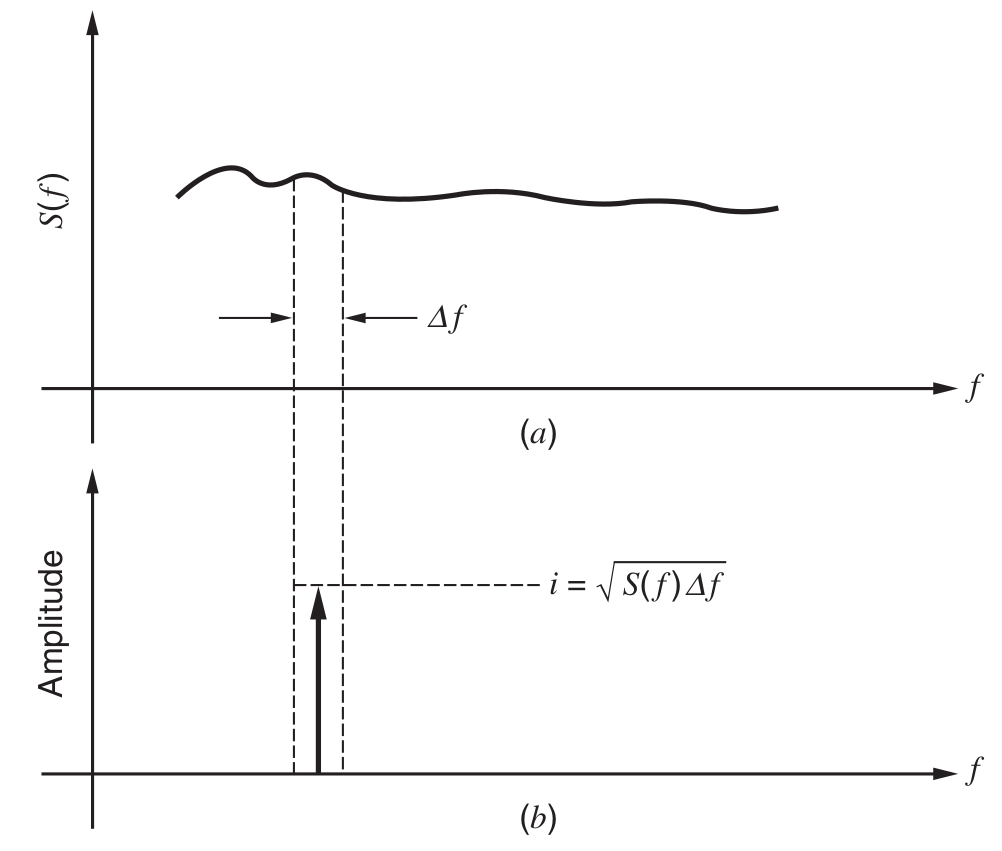
\includegraphics[width=0.5\textwidth]{figures/noise-eq-sin.png}
    \caption{Representation of noise in a bandwidth $\Delta f$ by an
    equivalent sinusoid with the same rms value.}
    \label{fig:noise-eq-sin}
\end{figure}

\section{Sources of noise}
\subsection{Thermal noise}
In conventional resistors, it is due to the \emph{random thermal motion of
the electrons} and is unnafected by the presence or absence of direct
current. In a resistor $R$, thermal noise can be represented by a series
voltage generator of mean square value $\mean{v^2}$ or by a shunt current
generator of mean square value $\mean{i^2}$
\begin{align*}
    \mean{v^2} &= 4kTR\Delta f, \\
    \mean{i^2} &= 4kT\frac{1}{R}\Delta f,
\end{align*}
where $k$ is the Boltzmann's constant, $T$ the absolute temperature (i.e. in
Kelvin) and $\Delta f$ the bandwidth in Hertz. This is illustrated in figure
\ref{fig:thermal-noise-repr}.
From this, it is clear that thermal noise is a \textbf{white noise}. Indeed,
its power spectral density is given either by $4kTR$ in \SI{}{\volt\squared
\per\hertz} or by $4kT\frac{1}{R}$ in \SI{}{\ampere\squared\per\hertz} and
is constant as a function of frequency (this is true up to \SI{1e13}{\hertz}).
Finally, the instantaneous amplitude distribution of thermal noise is
\textbf{Gaussian}.

\begin{figure}[ht]
    \centering
    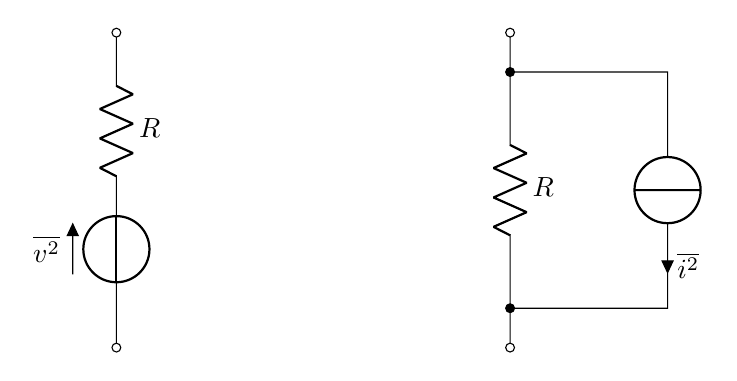
\begin{tikzpicture}
        \draw
        (0,0) to[short, o-] (0,-0.5)
        (0,-0.5) to[R, l=$R$] (0,-2)
        (0,-3.5) to[V, v=$\mean{v^2}$] (0,-2)
        (0,-3.5) to[short, -o] (0,-4)
        
        (5,0) to[short, o-*] (5,-0.5)
        (5,-0.5) to[R, l=$R$] (5,-3.5)
        (5,-3.5) to[short, *-o] (5,-4)
        (5,-0.5) -- (7,-0.5) to[I, i=$\mean{i^2}$] (7,-3.5) -- (5,-3.5)
        ;
    \end{tikzpicture}
    \caption{Representations of thermal noise. The noise voltage (resp. current) is
    represented by a sinusoidal voltage (resp. current) generator with rms value
    $v$ (resp $i$). 
    Note that, because the only quantity of interest is the mean-square value,
    the polarity of the sources doesn't matter.}
    \label{fig:thermal-noise-repr}
\end{figure}

\subsection{Shot noise}
Shot noise is always associated with a direct-current flow and is present in
diodes, MOS transistors and bipolar transistors (i.e. devices for which
a potential barrier across a junction exists). The passage of each carrier
across the junction can be modeled as a random event (which depends on
carrier's energy, direction, etc). The external current is thus composed of
a large number of random independent current pulses. Noting $I_J$ the average
current across the junction, the noise current has a mean square given by
\[ \mean{i^2} = 2qI_J\Delta f \]
where $q$ is the electronic charge. As for thermal noise, this is a
\textbf{white noise} with a \textbf{Gaussian} amplitude distribution.
A small-signal model of a diode including the effect of shot noise is
illustrated in figure~\ref{fig:shot-noise-diode-repr}.
Finally, shot noise is non-correlated with thermal noise. Because shot noise
and thermal noise are both Gaussian, this means that they are independent.

%TODO: why polarity of the source doesn't matter
\begin{figure}[ht]
    \centering
    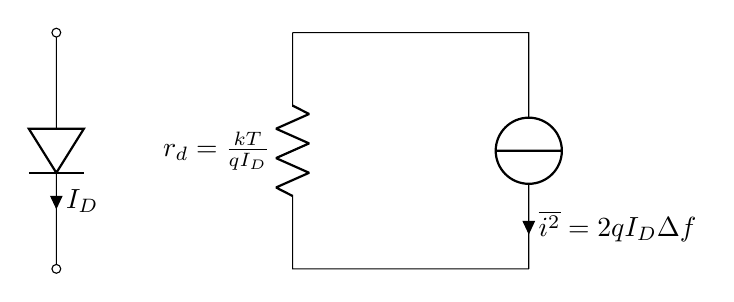
\begin{tikzpicture}
        \draw
        (2,0) to[short, o-] (2,-0.5)
        (2,-0.5) to[D, i=$I_D$] (2,-2.5)
        (2,-2.5) to[short, -o] (2,-3)
        
        (5,0) -- (8,0) to[I, i=$\mean{i^2}\equal2qI_D\Delta f$] (8,-3)
        (8,-3) -- (5,-3) to[R, l=$r_d\equal\frac{kT}{qI_D}$] (5,0)
        ;
    \end{tikzpicture}
    \caption{Diode small signal model including the effect of shot noise.
    Note that the small signal resistance $r_d$ of the diode is not an actual
    resistance (i.e. that's just a model of the diode). As such, it is not
    a source of thermal noise.}
    \label{fig:shot-noise-diode-repr}
\end{figure}

\subsection{Flicker noise}
Flicker noise (also called pink noise, or $1/f$ noise) is a type of noise
found in all active devices, as well as in some discrete passive elements
such as carbon resistors. The origins of flicker noise are varied, but it is
caused mainly by traps associated with contamination and crystal defects.
Flicker noise is always associated with a flow of direct current, the noise
current has a mean square given by
\[ \mean{i^2} = K_1\frac{I^a}{f^b}\Delta f \]
where $\Delta f$ is a small bandwidth around $f$\footnote{Indeed, remember
the discussion about equation~\eqref{eq:var-psd}.}, $I$ is the direct current,
$K_1$, $a$ and $b \approx 1$ are technology parameters.
At the opposite of thermal noise and shot noise, flicker noise is \textbf{not
white} (hence the name pink) and often has a \textbf{non-Gaussian} amplitude
distribution.

%TODO: might be better in a table in fact...
\subsection{Summary}
A summary of the different noise sources is given in
figure~\ref{fig:noise-summary}.

\begin{figure}[ht]
    \centering
    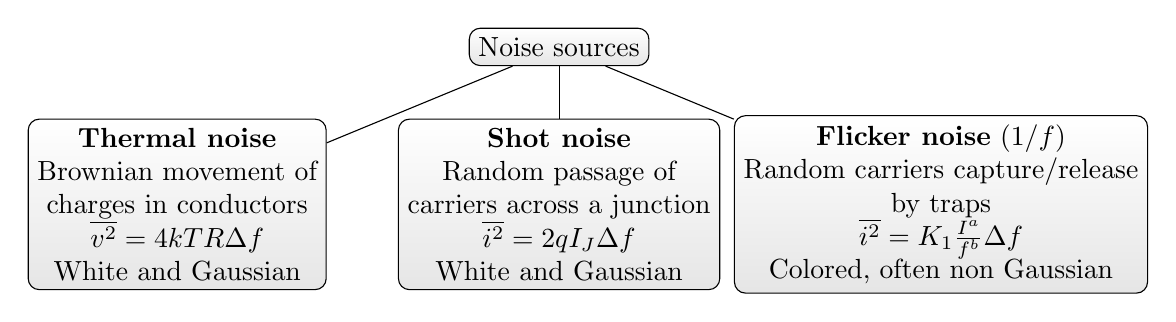
\begin{tikzpicture}[level distance=2cm,
        level 1/.style = {sibling distance = 0.4\textwidth},
        every node/.style = {shape=rectangle, rounded corners,
        draw, align=center,
        top color=white, bottom color=gray!20}]

        \node {Noise sources}
            child { node {\textbf{Thermal noise}\\
            Brownian movement of\\
            charges in conductors\\
            $\mean{v^2} = 4kTR\Delta f$\\
            White and Gaussian}  }
            child { node {\textbf{Shot noise}\\
            Random passage of\\
            carriers across a junction\\
            $\mean{i^2} = 2qI_J\Delta f$\\
            White and Gaussian} }
            child { node {\textbf{Flicker noise} ($1/f$)\\
            Random carriers capture/release\\
            by traps\\
            $\mean{i^2} = K_1\frac{I^a}{f^b}\Delta f$\\
            Colored, often non Gaussian} };    
    \end{tikzpicture}
    \caption{Summary of the different noise sources.}
    \label{fig:noise-summary}
\end{figure}

\section{Noise models of Integrated-Circuit Components}
\subsection{Resistors}
Monolithic and thin-film resistors display thermal noise. This has already
been illustrated in figure~\ref{fig:thermal-noise-repr}.

\subsection{Capacitors and inductors}
There are \emph{no sources of noise} in \emph{ideal} capacitors or
inductors. In practice, however, real components have parasitic resistances
that does display thermal noise.

\subsection{Junction Diode}
A small-signal model of the diode that includes the effect of shot noise was
already given in figure~\ref{fig:shot-noise-diode-repr}. This one, however,
does not take into account neither the series parasitic resistance of the
diode (which will display thermal noise) or flicker noise. A more complete
model is given in figure~\ref{fig:diode-noise-model}.

\begin{figure}[ht]
    \centering
    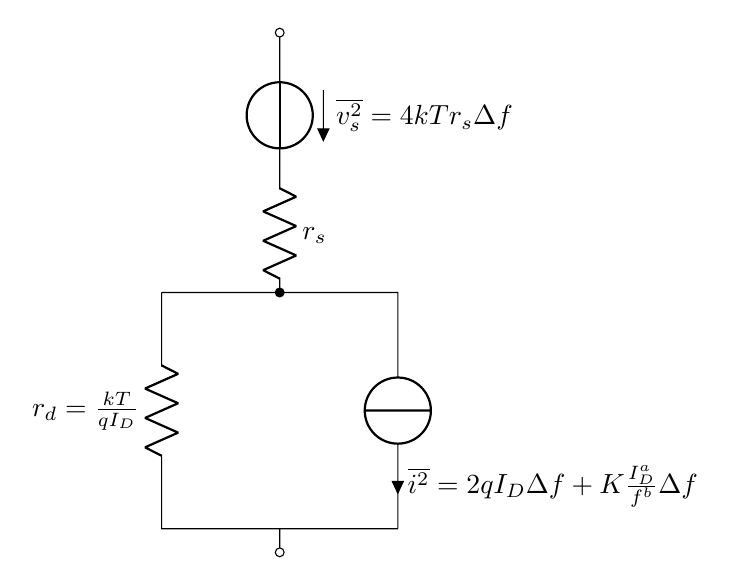
\begin{tikzpicture}
        \draw 
        (1.5, 3.3) to[short, o-] (1.5, 3) 
        (1.5, 3) to[V, v=$\mean{v^2_s}\equal4kTr_s\Delta f$] (1.5, 1.5)
        (1.5, 1.5) to[R, l=$r_s$] (1.5, 0) to[short, -*] (1.5, 0)
        (0,0) -- (3,0) to[I, i=$\mean{i^2}\equal2qI_D\Delta f
        + K\frac{I_D^a}{f^b}\Delta f$] (3,-3)
        (3,-3) -- (0,-3) to[R, l=$r_d\equal\frac{kT}{qI_D}$] (0,0)
        (1.5, -3) to[short, -o] (1.5, -3.3)
        ;
    \end{tikzpicture}
    \caption{Complete diode small-signal model equivalent circuit with noise
    sources.}
    \label{fig:diode-noise-model}
\end{figure}

Again, it is important to distinguish resistances that really exist from resistances that constitute
the model of the circuit component. In this case for instance, the parasitic series resistance
$r_s$ really exists, and as such exhibits thermal noise. The diode small signal resistance $r_d$ however
does not really exists, its purpose is purely to model the small-signal behaviour of the diode. As $r_d$
does not really exists, it obviously does not produce any kind of noise.

\subsection{Bipolar transistor}
A small-signal model equivalent circuit with noise sources for a bipolar transistor
is given in figure~\ref{fig:bjt-noise-model}. This model contains the following
noise sources:
\begin{enumerate}
	\item $\mean{v^2_b}$: thermal noise associated with the
	parasitic resistance of the base connection
	\[ \mean{v^2_b} = 4kTr_b\Delta f. \]
	\item $\mean{i^2_c}$: random transit time through the base (i.e. shot noise)
	\[ \mean{i^2_c} = 2qI_C\Delta f. \]
	\item $\mean{i^2_b}$: random carrier injection in emitter (i.e shot noise).
	Experimentally, it can also be seen that the base current is sensitive to
	flicker noise and telegraph noise (neglected in this course)
	\[ \mean{i^2_b} = 2qI_b\Delta f + K_1\frac{I_b^a}{f^b}\Delta f. \]
\end{enumerate}

\begin{figure}[ht]
    \centering
    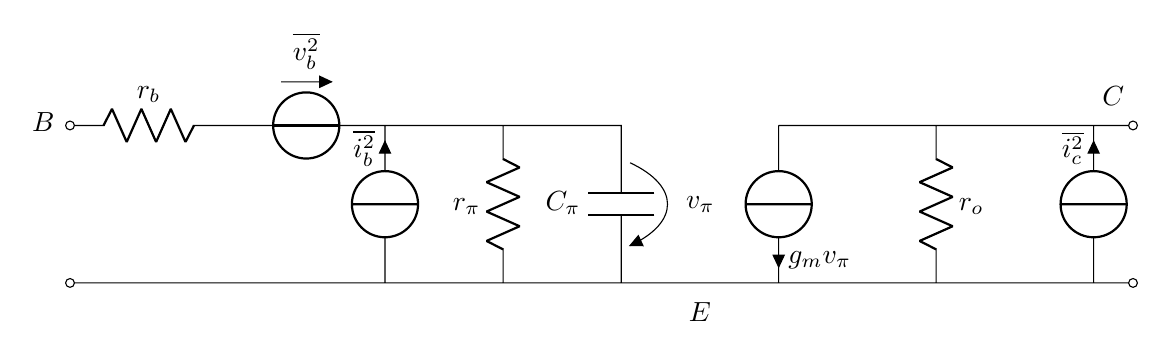
\begin{tikzpicture}
        \draw
        (0, 2) to[short, o-, l=$B$] (0, 2) to[R, l=$r_b$] (2, 2)
        (2, 2) to[V, v=$\mean{v_b^2}$] (4, 2)
        (0, 0) to[short, o-] (0, 0) -- (4, 0)
        (4, 0) to[I, i=$\mean{i_b^2}$] (4, 2)
        (4, 2) -- (5.5, 2) to[R, l_=$r_\pi$] (5.5, 0) -- (4, 0)
        (5.5, 2) -- (7, 2) to[C, l_=$C_\pi$, v^=$v_\pi$] (7, 0) -- (5.5, 0)
        (7, 0) to[short, -, l_=$E$] (9, 0)
        (9, 2) to[I, i=$g_mv_\pi$] (9, 0)
        (9, 2) -- (11, 2) to[R, l=$r_o$] (11, 0) -- (9, 0)
        (11, 0) -- (13, 0) to[I, i=$\mean{i_c^2}$] (13, 2) -- (11, 2)
        (13, 0) to[short, -o] (13.5, 0)
        (13, 2) to[short, -o, l=$C$] (13.5, 2)
        ;
    \end{tikzpicture}
    \caption{Bipolar transistor small-signal equivalent circuit
    with noise sources. Again, because $r_\pi$ and $r_o$ are not real resistance
    (i.e. they are there to model the physical behaviour of the device), they do not
    display thermal noise.}
    \label{fig:bjt-noise-model}
\end{figure}

The power spectral density associated with the noise source $\mean{i_b^2}$ (i.e
$\mean{i_b^2}/\Delta f$) is illustrated in figure~\ref{fig:corner-frequency}.
\begin{figure}
	\centering
	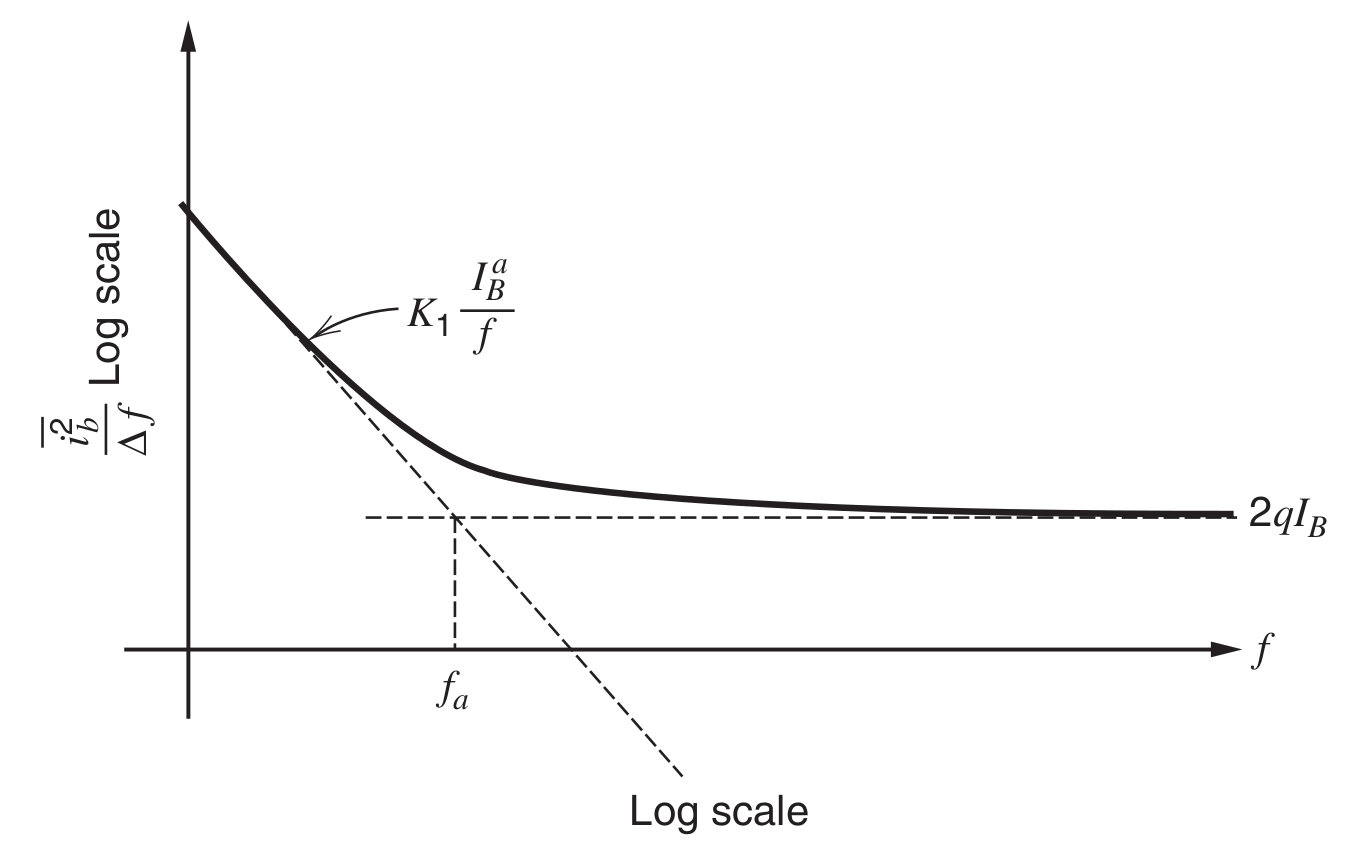
\includegraphics[width=0.6\textwidth]{figures/corner-frequency.png}
	\caption{Power spectral density of the base-current noise generator in a
	bipolar transistor. At low frequency, $1/f$ noise dominates while at higher
	frequency, shot noise dominates. $f_a$ is called the flicker noise
	\emph{corner} frequency.}
	\label{fig:corner-frequency}
\end{figure}

\subsection{MOS transistor}
A small-signal model equivalent circuit with noise sources for the MOS transistor
is given in figure~\ref{fig:mos-noise-model}. This model contains the following
noise sources:
\begin{enumerate}
    \item $\mean{i^2_g}$ : contains the shot noise generated by the gate leakage current
    \[ \mean{i^2_g} = 2qI_G\Delta f. \]
    At higher frequencies, another noise component due to a random component of the
    gate-to-channel voltage caused by thermal noise along the channel. This generates
    a noisy ac gate current $i_g$ with mean-squared value
    \[ \mean{i^2_g} = \frac{16}{15}kT\omega^2C^2_{gs}\Delta f. \]
    \item $\mean{i^2_d}$ : since the channel material is resistive, it exhibits thermal
    noise, which is a major source of noise in MOS transistors. Moreover, because MOS
    transistors conduct current near the gate-oxyde interface where surface states acts
    as traps that capture and release current carries: this generates flicker noise
    \[
        \mean{i^2_d} = 4kT\left(\frac{2}{3}g_m\right)\Delta f + K\frac{I_D^a}{f^b}\Delta f
    \]
    where $\frac{2}{3}g_m$ models the channel resistance.
\end{enumerate}

\begin{figure}[ht]
    \centering
    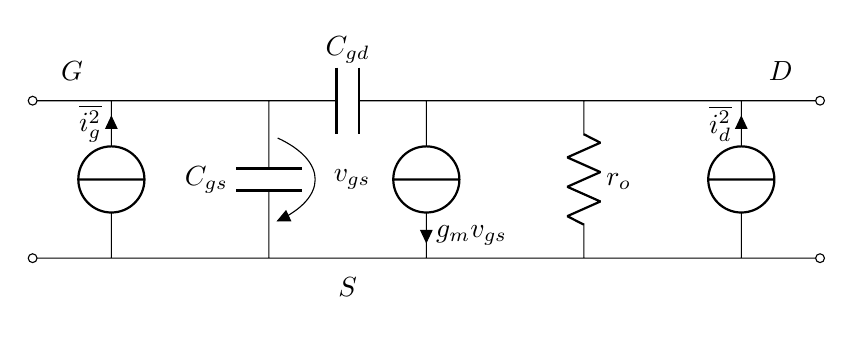
\begin{tikzpicture}
        \draw
        (0, 2) to[short, o-, l=$G$] (1, 2)
        (0, 0) to[short, o-] (1, 0) to[I, i=$\mean{i^2_g}$] (1,2)
        (1, 2) -- (3, 2) to[C, l_=$C_{gs}$, v^=$v_{gs}$] (3, 0) -- (1, 0)
        (3, 2) to[C, l^=$C_{gd}$] (5, 2) to[I, i=$g_mv_{gs}$] (5, 0)
        (5, 0) to[short, -, l^=$S$] (3, 0)
        (5, 2) -- (7, 2) to[R, l=$r_o$] (7, 0) -- (5, 0)
        (7, 0) -- (9, 0) to[I, i=$\mean{i^2_d}$] (9, 2) -- (7, 2)
        (9, 0) to[short, -o] (10, 0)
        (9, 2) to[short, -o, l^=$D$] (10, 2)
        ;
    \end{tikzpicture}
    \caption{The MOS transistor small-signal equivalent circuit
    with noise sources.}
    \label{fig:mos-noise-model}
\end{figure}

\section{Circuit noise calculations}
\subsection{Superposition}
When two sources of voltage noises are in series, they can be grouped
in a equivalent source of voltage noise $\mean{v^2_e}$ as illustrated
in figure~\ref{fig:superposition-voltage}.

\begin{figure}
    \centering
    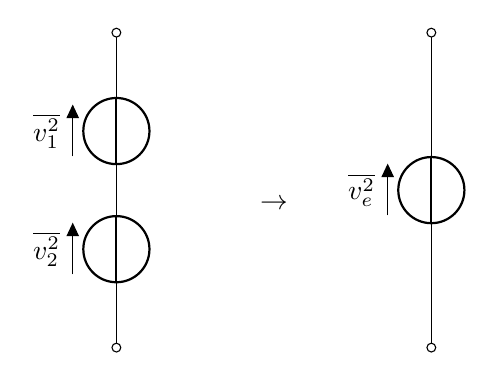
\begin{tikzpicture}
        \draw
        (0,0) to[short, o-] (0,-0.5)
        (0,-2) to[V, v=$\mean{v_1^2}$] (0,-0.5)
        (0,-3.5) to[V, v=$\mean{v_2^2}$] (0,-2)
        (0,-3.5) to[short, -o] (0,-4)
        
        (2,-2.5) node[label=$\to$]{}
        
        (4,0) to[short, o-] (4,-0.5)
        (4,-3.5) to[V, v=$\mean{v_e^2}$] (4,-0.5)
        (4,-3.5) to[short, -o] (4,-4)
        ;
    \end{tikzpicture}
    \caption{Superposition principle for noise voltage generators. A similar
    principle applies for noise current generators.}
    \label{fig:superposition-voltage}
\end{figure}
The relation between $\mean{v^2_e}$ and $\mean{v_1^2}$ and $\mean{v_2^2}$
depends on the relation between $v_1$ and $v_2$.

\begin{itemize}
    \item Non-correlated sources:
    \[ \mean{v^2_e} = \mean{v^2_1} + \mean{v^2_1} \]

    \item Fully correlated sources:
    \[ \mean{v^2_e} = \mean{(v_1+v_2)^2} \]

    \item Partially correlated sources:
    let $v_2 = v_{22} + v_{21}$ where $v_{22}$ is non-correlated with $v_1$
    and $v_{21}$ is fully correlated with $v_1$. In this case,
    \[ \mean{v^2_e} = \mean{(v_1 + v_{21})^2} + \mean{v^2_{22}}. \]
\end{itemize}

\subsection{Output noise}
Here are the steps involved in the computation of the total output noise
\begin{enumerate}
    \item Draw the small-signal equivalent circuit with noise sources ;
    \item Ignore the external input signal $v_i$ so that the output signal
    $v_o$ is due to noise generators only ;
    \item Apply the superposition principle and consider each noise source at
    a time. Perform the calculation as if each noise source were a sinusoid with
    rms value equal to that of the noise source being considered ;
    \item Combine every noise sources as explained in the previous section (i.e.,
    depending on their independence).
\end{enumerate}
A complete example can be found in~\cite[section~11.4.1]{gray}.

\subsection{Equivalent input noise and the minimum detectable signal}
\todo[inline]{This section could be improved. One idea would be to use the
complete example of the slides to explain concepts with an example. Also
need to define SNR, noise figure, noise temperature.}
The previous section showed us how to compute the output noise. The significance
of the noise performance of a circuit is, however, the limitation it places on
the smallest input signal the circuit can handle before the noise degrades the
quality of the output signal. For this reason, the noise performance is usually
expressed in terms of an equivalent input noise signal, which gives the same output
noise as the circuit under consideration.
The situation is illustrated in figure~\ref{fig:eq-input-noise}. The need for both
an equivalent input noise voltage generator and an equivalent input noise current
generator to represent the noise performance of the circuit for any source resistance
can be appreciated as follows. If $R_S = 0$, then $\mean{i^2_i}$ is shorted out, and
since the original circuit will still show output noise in general, we need an
equivalent input noise voltage $\mean{v^2_i}$ to represent this behavior. Similarly,,
if $R_S \to\infty$, then $\mean{v^2_i}$ cannot produce output noise, and since the
original circuit will still show output noise in general, we need an equivalent
input noise current $\mean{i^2_i}$ to represent this behavior.

\paragraph{Method}
In both cases, the output of both circuits (i.e. the original one and the one with
equivalent input noise generators) must be short-circuited.
\begin{enumerate}
    \item To obtain $\mean{v_i^2}$ : short-circuit the input of both circuits
    (as discussed above, this has for effect to remove the input noise current
    generator $\mean{i_i^2}$ effect) and equate $i_o$ in each case to obtain $v_i$.
    \item To obtain $\mean{i_i^2}$ : let open-circuited the input of both
    circuits (removing the input noise voltage generator $\mean{v_i^2}$ effect).
\end{enumerate}

Examples can be found in~\cite[sections~11.5.1-2]{gray} or in the slides.

\begin{figure}
    \centering
    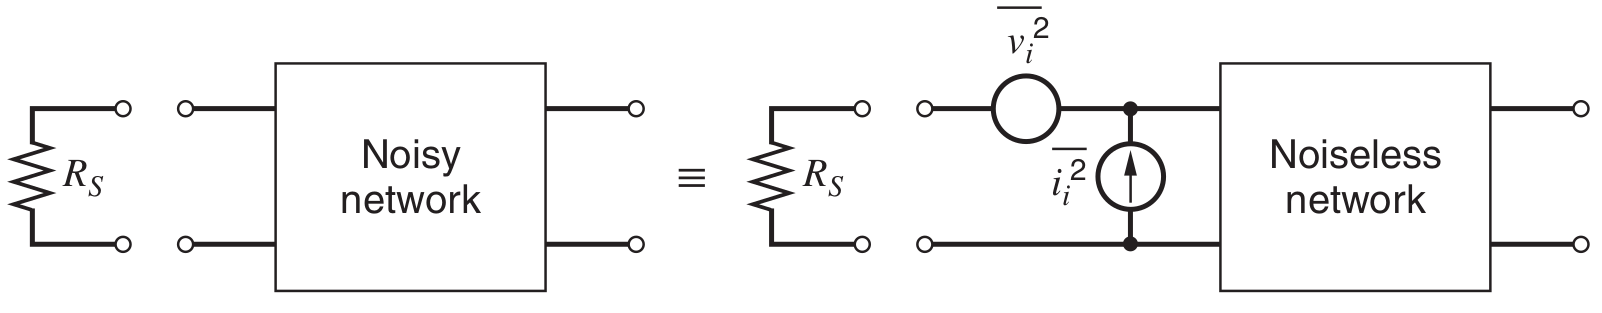
\includegraphics[width=0.75\textwidth]{figures/eq-input-noise.png}
    \caption{Representation of a noise in a two-port network equivalent input
    voltage and current generators.}
    \label{fig:eq-input-noise}
\end{figure}

\begin{mydef}[Minimum detectable signal]
    The minimum detectable signal (abbreviated MDS) can be taken as equal to
    the equivalent input noise voltage in the passband of the circuit under
    consideration.
\end{mydef}

\todo[inline]{Noise bandwidth}

\part{Active filters}
The reference for this part is~\cite[chapter~11]{sedra}.
\section{First-order filters}
\subsection{Low-pass filter}
The voltage (or current) transfer function of a first-order low-pass
filter is given by
\[ H(\Omega) = \frac{H_0}{1+j\Omega} \]
where $H_0$ is the DC gain (i.e. $H(0) = H_0$) and $\Omega = \frac{\omega}{
\omega_c}$ is the pulsation normalized by the cut-off frequency $\omega_c$. The
power transfer function is then simply given by $|H(\Omega)|^2$.
\subsection{High-pass filter}
The voltage (or current) transfer function of a first-order high-pass
filter is given by
\[ H(\Omega) = H_0\frac{j\Omega}{1+j\Omega}. \]
Note that in this case $H_0$ is the high frequency gain.

\subsection{Implementation}
A first-order low-pass filter can be implemented by a simple circuit illustrated
in figure~\ref{fig:1st-order-lp}. The corresponding voltage transfer function
is given by
\[ H(\omega) = \frac{v_{out}}{v_{in}} = \left(1+\frac{R_2}{R_1}\right)
\frac{1}{1+j\omega RC}.\]
To obtain a first-order high-pass filter, one simply needs to switch $R$ and $C$
on the schematic of figure~\ref{fig:1st-order-lp}. By identification with the
canonical form of a first-order low-pass filter, we find
\begin{align*}
    H_0 &= 1+\frac{R_2}{R_1} &
    \omega_c &= \frac{1}{RC}.
\end{align*}

\begin{figure}
    \centering
    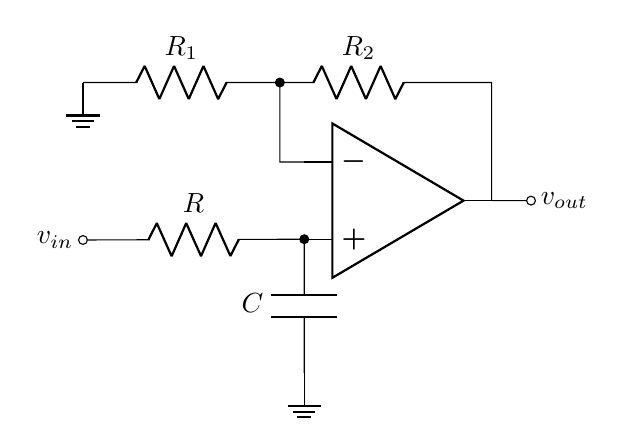
\begin{tikzpicture}
        \draw
        (4,0.5) node [op amp] (opamp) {}
        (0,0) node [left] {$v_{in}$} to [R, l=$R$, o-] (opamp.+)
        -- (opamp.+) to [C, l_=$C$, *-] ($(opamp.+)+(0,-1.7)$) node [ground] {} 
        (opamp.-) -| (2.5,2)
        (2.5,2) to [R, l_=$R_1$, *-] (0, 2) node [ground] {}
        (2.5,2) to [R, l=$R_2$] (4.5,2)
        (opamp.out) |- (4.5, 2)
        (opamp.out) to[short, -o] ($(opamp.out)+(0.5,0)$) node [right] {$v_{out}$}
        ;
    \end{tikzpicture}
    \caption{Implementation of a first-order low-pass filter.}
    \label{fig:1st-order-lp}
\end{figure}

\section{Second-order filters}
The voltage (or current) transfer function of a second-order low-pass filter is given by
\[ H(\Omega) = \frac{H_0}{1+2\zeta(j\Omega) + (j\Omega)^2} \]
where $H_0$ is again the static gain, $\zeta$ is the damping factor and $\Omega
= \frac{\omega}{\omega_n}$ is the pulsation normalized by the undamped natural pulsation
$\omega_n$. The meaning of $\zeta$ and $\omega_n$ can be understood by noting that
\[ |H(1)| = \frac{1}{2\zeta} \eqdef Q \]
where $Q$ is what we call the \emph{quality factor} of a filter.
As reminder from the linear control course, the effect of $\zeta$ on the transfer
function as well as on the transient response to a unit step is illustrated in
figures~\ref{fig:zeta-impact-on-magn}, \ref{fig:zeta-impact-on-phase} and
\ref{fig:zeta-impact-on-step-response}. It can be seen from those figures that there
is a trade-off between oscillations and settling time. With a damping ratio too high,
you'll not get any oscillation but the settling time will be high. A damping ratio
around 0.7 is generally a good trade-off.

\begin{figure}
    \centering
    \resizebox{0.75\textwidth}{!}{% This file was created by matlab2tikz.
%
%The latest updates can be retrieved from
%  http://www.mathworks.com/matlabcentral/fileexchange/22022-matlab2tikz-matlab2tikz
%where you can also make suggestions and rate matlab2tikz.
%
\definecolor{mycolor1}{rgb}{0.00000,0.75000,0.75000}%
\definecolor{mycolor2}{rgb}{0.75000,0.00000,0.75000}%
\definecolor{mycolor3}{rgb}{0.75000,0.75000,0.00000}%
%
\begin{tikzpicture}

\begin{axis}[%
width=5.081in,
height=1.75in,
at={(0.852in,0.511in)},
scale only axis,
separate axis lines,
every outer x axis line/.append style={black},
every x tick label/.append style={font=\color{black}},
xmode=log,
xmin=0.01,
xmax=100,
xminorticks=true,
xlabel={$\text{Normalized frequency }\Omega$},
xmajorgrids,
every outer y axis line/.append style={black},
every y tick label/.append style={font=\color{black}},
ymin=-60,
ymax=45,
ylabel={Mag (dB)},
ymajorgrids,
yminorgrids,
axis background/.style={fill=white},
legend style={legend cell align=left,align=left,draw=black}
]
\addplot [color=blue,solid,line width=2.0pt]
  table[row sep=crcr]{%
0.01	0.000864288584785583\\
0.0100926219098705	0.000880373949364043\\
0.0101861017015598	0.000896758695629902\\
0.0102804473209331	0.000913448396268715\\
0.0103756667874519	0.000930448727715268\\
0.0104717681948552	0.0009477654720848\\
0.010568759711848	0.00096540451914846\\
0.0106666495827954	0.000983371868339501\\
0.0107654461284232	0.00100167363077477\\
0.0108651577465254	0.00102031603137634\\
0.0109657929126781	0.00103930541094098\\
0.0110673601809597	0.0010586482283444\\
0.0111698681846782	0.0010783510627107\\
0.0112733256371049	0.00109842061566455\\
0.0113777413322149	0.00111886371360642\\
0.0114831241454351	0.0011396873100454\\
0.0115894830343981	0.00116089848796664\\
0.0116968270397039	0.00118250446223713\\
0.011805165285688	0.00120451258205957\\
0.0119145069811978	0.00122693033349154\\
0.0120248614203741	0.0012497653419742\\
0.0121362379834424	0.0012730253749494\\
0.0122486461375093	0.00129671834448436\\
0.0123620954373677	0.00132085230999444\\
0.0124765955263087	0.00134543548095031\\
0.0125921561369415	0.00137047621971594\\
0.0127087870920206	0.00139598304435551\\
0.0128264983052806	0.00142196463157511\\
0.0129452997822792	0.00144842981964868\\
0.0130652016212472	0.00147538761144202\\
0.0131862140139475	0.00150284717747902\\
0.0133083472465408	0.00153081785905956\\
0.0134316117004602	0.0015593091714543\\
0.0135560178532937	0.00158833080713577\\
0.0136815762796747	0.0016178926390824\\
0.0138082976521809	0.00164800472414973\\
0.0139361927422414	0.00167867730648169\\
0.0140652724210524	0.00170992082102767\\
0.014195547660501	0.00174174589707071\\
0.0143270295340983	0.00177416336186711\\
0.0144597292179202	0.00180718424433776\\
0.0145936579915576	0.00184081977880723\\
0.014728827239075	0.00187508140885612\\
0.0148652484499786	0.00190998079121357\\
0.0150029332201922	0.00194552979972437\\
0.0151418932530435	0.00198174052940434\\
0.0152821403602587	0.00201862530056074\\
0.0154236864629663	0.00205619666299508\\
0.0155665435927106	0.00209446740027281\\
0.0157107238924745	0.0021334505340986\\
0.0158562396177114	0.00217315932873712\\
0.016003103137387	0.00221360729555876\\
0.0161513269350309	0.00225480819761727\\
0.0163009236097974	0.00229677605437538\\
0.0164519058775366	0.00233952514645467\\
0.0166042865718753	0.00238307002054487\\
0.0167580786453077	0.00242742549432192\\
0.0169132951702965	0.00247260666153704\\
0.0170699493403841	0.00251862889714724\\
0.0172280544713139	0.00256550786256082\\
0.0173876240021625	0.00261325951099765\\
0.0175486714964815	0.00266190009291212\\
0.0177112106434509	0.00271144616154836\\
0.0178752552590424	0.00276191457858106\\
0.0180408192871938	0.00281332251988465\\
0.0182079168009946	0.00286568748137844\\
0.0183765620038817	0.00291902728500575\\
0.018546769230847	0.00297336008481978\\
0.0187185529496558	0.00302870437317836\\
0.0188919277620767	0.00308507898705302\\
0.0190669084051225	0.00314250311446037\\
0.0192435097523033	0.00320099630102507\\
0.0194217468148903	0.00326057845663797\\
0.0196016347431919	0.00332126986225932\\
0.0197831888278416	0.00338309117686319\\
0.0199664245010979	0.00344606344445953\\
0.0201513573381556	0.00351020810130737\\
0.0203380030584698	0.00357554698324015\\
0.0205263775270925	0.00364210233310129\\
0.0207164967560207	0.00370989680837072\\
0.0209083769055575	0.00377895348888215\\
0.021102034285686	0.00384929588473518\\
0.0212974853574552	0.0039209479443114\\
0.0214947467343798	0.00399393406245821\\
0.0216938351838518	0.00406827908884786\\
0.0218947676285662	0.00414400833645575\\
0.022097561147959	0.00422114759020621\\
0.0223022329796594	0.00429972311581247\\
0.0225088005209546	0.00437976166874343\\
0.0227172813302691	0.00446129050337874\\
0.0229276931286565	0.00454433738232127\\
0.0231400538013065	0.00462893058591313\\
0.0233543813990648	0.00471509892188959\\
0.0235706941399673	0.00480287173524794\\
0.0237890104107889	0.00489227891828483\\
0.0240093487686065	0.00498335092082907\\
0.024231727942376	0.00507611876066389\\
0.0244561668345245	0.00517061403413474\\
0.0246826845225569	0.00526686892697906\\
0.0249113002606779	0.00536491622533946\\
0.025142033481428	0.00546478932699664\\
0.0253749037973357	0.00556652225280271\\
0.0256099310025846	0.00567014965833022\\
0.0258471350746956	0.00577570684575975\\
0.0260865361762255	0.00588322977595786\\
0.0263281546564802	0.00599275508080679\\
0.0265720110532451	0.00610432007576842\\
0.0268181260945302	0.0062179627726631\\
0.0270665207003324	0.006333721892692\\
0.0273172159844138	0.00645163687974518\\
0.0275702332560958	0.00657174791390274\\
0.0278255940220712	0.00669409592521549\\
0.0280833199882317	0.00681872260776879\\
0.0283434330615131	0.00694567043395428\\
0.0286059553517574	0.00707498266907432\\
0.0288709091735924	0.00720670338616928\\
0.0291383170483279	0.00734087748117131\\
0.0294082017058706	0.00747755068829191\\
0.029680586086656	0.0076167695957375\\
0.0299554933435981	0.00775858166172752\\
0.0302329468440578	0.0079030352307648\\
0.0305129701718287	0.00805017955027343\\
0.0307955871291423	0.00820006478751328\\
0.0310808217386906	0.00835274204681903\\
0.0313686982456688	0.00850826338717679\\
0.0316592411198352	0.00866668184012455\\
0.0319524750575921	0.00882805142798956\\
0.0322484249840844	0.00899242718247181\\
0.0325471160553185	0.00915986516358302\\
0.0328485736603004	0.00933042247893473\\
0.0331528234231942	0.00950415730340421\\
0.0334598912054997	0.00968112889916204\\
0.0337698031082509	0.0098613976360728\\
0.0340825854742345	0.0100450250125105\\
0.0343982648902292	0.0102320736765325\\
0.0347168681892656	0.0104226074474749\\
0.0350384224529068	0.0106166913379596\\
0.0353629550135504	0.0108143915762983\\
0.0356904934567523	0.0110157756293551\\
0.0360210656235707	0.0112209122258035\\
0.0363546996129332	0.0114298713798574\\
0.0366914237840249	0.0116427244154344\\
0.0370312667586993	0.0118595439907782\\
0.0373742574239106	0.0120804041235651\\
0.03772042493417	0.0123053802164654\\
0.0380697987140229	0.0125345490832141\\
0.0384224084605506	0.0127679889751517\\
0.0387782841458946	0.0130057796082852\\
0.0391374560198038	0.0132480021908765\\
0.0394999546122064	0.0134947394515226\\
0.0398658107358044	0.0137460756677985\\
0.0402350554886929	0.0140020966954506\\
0.0406077202570037	0.0142628899981079\\
0.0409838367175726	0.0145285446776064\\
0.0413634368406327	0.0147991515048638\\
0.0417465528925314	0.015074802951356\\
0.0421332174384729	0.0153555932211862\\
0.0425234633452868	0.0156416182837722\\
0.0429173237842216	0.0159329759071587\\
0.043314832233764	0.0162297656919689\\
0.043716022482485	0.0165320891059973\\
0.0441209286319119	0.0168400495194717\\
0.0445295850994266	0.0171537522409986\\
0.0449420266211914	0.0174733045541803\\
0.0453582882551019	0.0177988157549332\\
0.0457784053837662	0.0181303971895622\\
0.0462024137175131	0.0184681622935016\\
0.0466303492974273	0.0188122266308588\\
0.0470622484984128	0.019162707934685\\
0.047498148032285	0.0195197261480293\\
0.0479380849508911	0.01988340346578\\
0.0483820966492596	0.0202538643773216\\
0.0488302208687788	0.020631235710007\\
0.0492824957004051	0.0210156466734625\\
0.0497389595879006	0.0214072289047537\\
0.0501996513311008	0.0218061165144299\\
0.0506646100892127	0.0222124461334357\\
0.0511338753841433	0.0226263569609696\\
0.0516074871038591	0.0230479908132113\\
0.0520854855057766	0.0234774921730587\\
0.0525679112201842	0.0239150082407669\\
0.0530548052536957	0.0243606889856081\\
0.0535462089927361	0.0248146871985311\\
0.0540421642070592	0.02527715854581\\
0.0545427130532983	0.025748261623779\\
0.0550478980785497	0.0262281580146076\\
0.0555577622239888	0.0267170123431704\\
0.0560723488285203	0.0272149923350051\\
0.0565917016324624	0.0277222688754263\\
0.0571158647812643	0.0282390160697844\\
0.0576448828292588	0.0287654113048838\\
0.0581788007434494	0.0293016353116291\\
0.0587176639073326	0.0298478722288765\\
0.0592615181247555	0.0304043096685399\\
0.0598104096238094	0.0309711387819771\\
0.0603643850607587	0.0315485543276765\\
0.0609234915240071	0.0321367547402665\\
0.0614877765381002	0.0327359422008893\\
0.062057288067765	0.0333463227089498\\
0.0626320745219869	0.0339681061552898\\
0.0632121847581246	0.0346015063967842\\
0.0637976680860628	0.0352467413324351\\
0.0643885742724042	0.0359040329809429\\
0.0649849535446989	0.0365736075598213\\
0.0655868565957143	0.0372556955660916\\
0.0661943345877439	0.0379505318585573\\
0.0668074391569562	0.0386583557416984\\
0.0674262224177834	0.0393794110512708\\
0.0680507369673521	0.0401139462415778\\
0.068681035889953	0.0408622144744784\\
0.0693171727615541	0.0416244737101878\\
0.0699592016543538	0.0424009867998611\\
0.0706071771413777	0.043192021580049\\
0.0712611543011175	0.0439978509690464\\
0.0719211887222119	0.0448187530651473\\
0.0725873365081725	0.0456550112468677\\
0.0732596542821523	0.0465069142752171\\
0.0739381991917587	0.0473747563979901\\
0.0746230289139111	0.0482588374561627\\
0.0753142016597437	0.0491594629924526\\
0.0760117761795533	0.0500769443620421\\
0.076715811767793	0.0510115988455492\\
0.0774263682681127	0.0519637497643105\\
0.0781435060784454	0.0529337265979614\\
0.0788672861561415	0.0539218651044093\\
0.0795977700231499	0.0549285074422819\\
0.0803350197712474	0.0559540022958312\\
0.0810790980673169	0.0569987050023735\\
0.0818300681586739	0.0580629776824006\\
0.0825879938784427	0.0591471893722573\\
0.0833529396509819	0.060251716159621\\
0.0841249704973612	0.0613769413216983\\
0.0849041520408875	0.0625232554663137\\
0.0856905505126835	0.0636910566758689\\
0.0864842327573172	0.0648807506542746\\
0.0872852662384838	0.0660927508769467\\
0.0880937190447399	0.0673274787438606\\
0.0889096598952916	0.0685853637358266\\
0.0897331581458352	0.0698668435739735\\
0.0905642837944529	0.0711723643825894\\
0.0914031074875623	0.0725023808553093\\
0.0922497005259217	0.0738573564248268\\
0.0931041348706907	0.0752377634361169\\
0.0939664831495469	0.0766440833233218\\
0.0948368186628592	0.0780768067903308\\
0.0957152153899187	0.0795364339951875\\
0.0966017479952265	0.0810234747383509\\
0.0974964918348409	0.0825384486549926\\
0.0983995229627823	0.0840818854113126\\
0.099310918137498	0.0856543249050553\\
0.100230754828387	0.0872563174703057\\
0.101159111222383	0.0888884240866067\\
0.102096066230605	0.0905512165926063\\
0.103041699495059	0.0922452779042326\\
0.103996091395412	0.0939712022375834\\
0.104959323055823	0.0957295953366117\\
0.105931476351837	0.0975210747057128\\
0.106912633917348	0.0993462698473618\\
0.107902879151618	0.101205822504869\\
0.108902296226373	0.103100386910475\\
0.10991097009295	0.105030630038772\\
0.110928986489522	0.106997231865747\\
0.111956431948388	0.109000885633426\\
0.112993393803322	0.111042298120385\\
0.114039960197003	0.113122189918191\\
0.115096220088503	0.115241295713956\\
0.11616226326085	0.117400364579142\\
0.11723818032866	0.119600160264797\\
0.118324062745838	0.121841461503349\\
0.119420002813353	0.124125062317136\\
0.120526093687084	0.126451772333864\\
0.121642429385737	0.128822417109144\\
0.122769104798836	0.131237838456287\\
0.123906215694792	0.133698894783573\\
0.125053858729039	0.136206461439123\\
0.126212131452255	0.138761431063679\\
0.127381132318648	0.141364713951365\\
0.12856096069433	0.14401723841874\\
0.129751716865759	0.146719951182317\\
0.130953502048267	0.149473817744767\\
0.132166418394661	0.15227982279005\\
0.133390569003906	0.155138970587724\\
0.134626057929891	0.158052285406622\\
0.135872990190271	0.161020811938228\\
0.137131471775394	0.164045615729942\\
0.138401609657313	0.167127783628527\\
0.139683511798874	0.170268424234038\\
0.140977287162897	0.173468668364477\\
0.142283045721435	0.176729669531491\\
0.143600898465126	0.180052604427441\\
0.144930957412622	0.183438673424077\\
0.146273335620113	0.186889101083249\\
0.147628147190939	0.190405136679898\\
0.148995507285285	0.193988054737735\\
0.150375532129974	0.197639155577923\\
0.151768339028341	0.201359765881148\\
0.153174046370208	0.205151239263487\\
0.154592773641948	0.209014956866402\\
0.156024641436637	0.212952327961339\\
0.157469771464309	0.216964790569315\\
0.158928286562298	0.221053812095924\\
0.160400310705682	0.225220889982243\\
0.16188596901782	0.229467552372075\\
0.163385387780986	0.233795358796033\\
0.164898694447106	0.238205900872947\\
0.16642601764859	0.242700803029149\\
0.167967487209265	0.247281723236103\\
0.169523234155412	0.251950353767005\\
0.171093390726901	0.2567084219729\\
0.172678090388436	0.261557691078908\\
0.174277467840892	0.266499961001165\\
0.175891659032773	0.271537069185161\\
0.177520801171763	0.276670891466091\\
0.17916503273639	0.281903342951934\\
0.180824493487795	0.287236378929968\\
0.182499324481615	0.292671995797448\\
0.184189668079971	0.298212232017251\\
0.185895667963569	0.303859169099222\\
0.187617469143912	0.309614932608113\\
0.18935521797563	0.315481693198932\\
0.191109062168914	0.321461667680605\\
0.192879150802078	0.32755712010888\\
0.194665634334226	0.333770362909433\\
0.196468664618045	0.340103758032156\\
0.198288394912707	0.346559718137699\\
0.200124979896904	0.35314070781732\\
0.201978575681988	0.359849244847175\\
0.203849339825246	0.366687901478192\\
0.205737431343291	0.37365930576279\\
0.207643010725577	0.380766142919652\\
0.209566239948043	0.38801115673791\\
0.21150728248688	0.395397151022072\\
0.213466303332424	0.402926991079132\\
0.215443469003188	0.410603605249371\\
0.217438947560008	0.418429986482335\\
0.219452908620331	0.426409193959655\\
0.221485523372636	0.434544354766354\\
0.22353696459098	0.442838665612407\\
0.225607406649686	0.451295394606352\\
0.227697025538168	0.459917883082901\\
0.229805998875885	0.468709547486463\\
0.231934505927443	0.477673881312732\\
0.234082727617829	0.486814457110433\\
0.236250846547795	0.496134928545495\\
0.238439047009372	0.505639032530067\\
0.240647515001542	0.515330591418745\\
0.242876438246045	0.525213515274641\\
0.245126006203334	0.53529180420798\\
0.247396410088681	0.545569550790008\\
0.249687842888433	0.556050942545179\\
0.252000499376409	0.566740264524667\\
0.254334576130465	0.577641901964473\\
0.256690271549195	0.588760343031397\\
0.259067785868801	0.600100181660537\\
0.261467321180109	0.61166612048788\\
0.263889081445751	0.623462973881936\\
0.266333272517498	0.635495671078457\\
0.268800102153761	0.64776925942245\\
0.271289780037247	0.660288907722011\\
0.273802517792786	0.673059909718601\\
0.276338529005317	0.68608768767872\\
0.278898029238044	0.699377796112076\\
0.281481236050758	0.712935925621726\\
0.28408836901833	0.726767906891829\\
0.286719649749377	0.740879714819001\\
0.289375301905095	0.755277472793541\\
0.292055551218275	0.769967457137156\\
0.294760625512486	0.784956101704094\\
0.297490754721444	0.800250002653042\\
0.300246170908555	0.815855923397431\\
0.30302710828664	0.831780799742315\\
0.305833803237843	0.848031745216291\\
0.308666494333727	0.864616056607513\\
0.311525422355549	0.881541219713278\\
0.314410830314726	0.898814915313168\\
0.317322963473498	0.916445025376314\\
0.320262069365765	0.934439639513972\\
0.323228397818138	0.952807061689093\\
0.326222200971167	0.971555817195427\\
0.329243733300777	0.990694659919211\\
0.332293251639897	1.01023257989742\\
0.335371015200293	1.03017881118721\\
0.338477285594598	1.05054284006218\\
0.341612326858553	1.07133441355191\\
0.344776405473446	1.09256354834215\\
0.347969790388769	1.11424054005433\\
0.351192753045073	1.13637597292382\\
0.354445567397043	1.15898072989787\\
0.357728509936787	1.18206600317525\\
0.361041859717334	1.20564330521108\\
0.364385898376354	1.22972448021172\\
0.367760910160103	1.25432171614629\\
0.371167181947576	1.27944755730282\\
0.374605003274899	1.30511491741922\\
0.378074666359935	1.33133709342074\\
0.381576466127125	1.35812777979819\\
0.385110700232557	1.38550108366282\\
0.388677669089267	1.4134715405168\\
0.392277675892772	1.44205413078039\\
0.395911026646846	1.47126429711974\\
0.399578030189527	1.50111796262261\\
0.403278998219371	1.53163154987197\\
0.407014245321944	1.56282200097158\\
0.410784088996565	1.59470679858083\\
0.414588849683291	1.62730398802073\\
0.418428850790158	1.66063220051697\\
0.422304418720667	1.6947106776511\\
0.426215882901532	1.72955929709566\\
0.430163575810679	1.76519859971524\\
0.434147833005509	1.80164981812095\\
0.438168993151419	1.83893490677309\\
0.44222739805059	1.87707657373329\\
0.446323392671039	1.9160983141759\\
0.450457325175946	1.95602444577642\\
0.45462954695324	1.99688014610445\\
0.458840412645476	2.03869149215846\\
0.463090280179974	2.08148550219098\\
0.467379510799246	2.12529017998483\\
0.471708469091702	2.1701345617542\\
0.476077523022637	2.21604876585887\\
0.480487043965513	2.26306404553582\\
0.484937406733524	2.31121284486979\\
0.489428989611453	2.36052885824345\\
0.493962174387832	2.41104709352895\\
0.498537346387389	2.46280393930551\\
0.503154894503805	2.51583723641354\\
0.507815211232767	2.57018635418325\\
0.512518692705333	2.62589227170748\\
0.517265738721602	2.68299766456184\\
0.522056752784698	2.74154699741394\\
0.526892142135067	2.80158662300487\\
0.531772317785097	2.86316488803298\\
0.536697694554048	2.92633224652156\\
0.541668691103315	2.99114138130955\\
0.546685729972018	3.05764733436849\\
0.551749237612913	3.12590764672006\\
0.556859644428641	3.19598250880849\\
0.562017384808319	3.26793492227118\\
0.567222897164454	3.34183087415014\\
0.572476623970218	3.41773952469943\\
0.57777901179705	3.49573341006846\\
0.583130511352622	3.57588866128273\\
0.588531577519145	3.65828524110236\\
0.593982669392036	3.74300720051767\\
0.599484250318941	3.83014295684421\\
0.605036787939122	3.91978559560795\\
0.610640754223204	4.01203319867159\\
0.616296625513294	4.10698920134722\\
0.622004882563471	4.20476278157558\\
0.62776601058065	4.30546928463383\\
0.633580499265825	4.40923068726863\\
0.639448842855694	4.51617610564869\\
0.64537154016467	4.62644235209984\\
0.65134909462728	4.74017454623768\\
0.657382014340959	4.85752678686222\\
0.663470812109235	4.97866289183933\\
0.669616005485322	5.10375721418615\\
0.675818116816111	5.23299554372098\\
0.682077673286569	5.36657610495896\\
0.68839520696455	5.50471066346235\\
0.694771254846024	5.6476257546207\\
0.701206358900718	5.79556405088331\\
0.707701066118189	5.94878588583695\\
0.714255928554313	6.10757095626816\\
0.720871503378214	6.27222022652884\\
0.727548352919623	6.44305806319812\\
0.734287044716676	6.62043463227084\\
0.741088151564157	6.80472859596751\\
0.747952251562182	6.99635015181369\\
0.754879928165344	7.19574446291663\\
0.761871770232299	7.40339553537333\\
0.768928372075831	7.61983060640036\\
0.776050333513357	7.84562511486997\\
0.78323825991792	8.08140833402831\\
0.790492762269642	8.32786975342894\\
0.797814457207663	8.58576630206146\\
0.805203967082547	8.85593050474124\\
0.812661920009195	9.1392796547249\\
0.82018894992022	9.43682605996082\\
0.827785696619848	9.74968836621622\\
0.835452805838287	10.079103857217\\
0.843190929286626	10.4264414458571\\
0.851000724712225	10.7932147442475\\
0.858882855954625	11.1810940371834\\
0.866837993001978	11.591915019202\\
0.874866812047991	12.0276805090493\\
0.882969995549409	12.4905485454837\\
0.89114823228402	12.9827954675913\\
0.899402217409204	13.5067343761921\\
0.907732652521023	14.0645553763747\\
0.916140245713852	14.658030340154\\
0.924625711640574	15.2879858062413\\
0.933189771573324	15.953386083531\\
0.941833153464795	16.6497822445592\\
0.95055659201012	17.3667954004673\\
0.959360828709314	18.0843276083681\\
0.968246611930312	18.7676669464685\\
0.977214696972572	19.3632453798472\\
0.986265846131282	19.799959067039\\
0.995400828762152	20.0032806323958\\
1.00462042134681	19.9232005523158\\
1.01392540755882	19.5597188267987\\
1.02331657833024	18.9628449794468\\
1.03279473191895	18.2071063859079\\
1.0423606739764	17.3636068876475\\
1.05201521761616	16.4859145195863\\
1.061759183483	15.6087412035182\\
1.07159339982267	14.7521848823298\\
1.08151870255229	13.92662444488\\
1.09153593533139	13.1365088186325\\
1.10164594963366	12.382873694693\\
1.11184960481927	11.6648925343502\\
1.12214776820798	10.9807934655893\\
1.13254131515281	10.3283863833215\\
1.14303112911448	9.70535818672702\\
1.15361810173648	9.10943253671947\\
1.16430313292088	8.53845139454071\\
1.17508713090481	7.99041194144466\\
1.18597101233767	7.4634784828942\\
1.19695570235904	6.9559807340939\\
1.20804213467733	6.46640508293292\\
1.21923125164911	5.99338261651738\\
1.23052400435926	5.5356760511213\\
1.24192135270178	5.0921667409775\\
1.2534242654614	4.66184237813756\\
1.2650337203959	4.24378566934484\\
1.27675070431927	3.83716408978406\\
1.28857621318552	3.44122071046557\\
1.30051125217341	3.05526604183581\\
1.31255683577184	2.67867081064863\\
1.32471398786612	2.31085957803173\\
1.33698374182495	1.95130510676864\\
1.34936714058831	1.59952339076231\\
1.36186523675608	1.25506926690549\\
1.37447909267754	0.917532537672574\\
1.38720978054162	0.586534540843135\\
1.4000583824681	0.261725110422307\\
1.41302599059953	-0.0572201201690564\\
1.42611370719413	-0.370602115282841\\
1.43932264471941	-0.67870057170564\\
1.45265392594678	-0.981775823024146\\
1.46610868404698	-1.28007054168769\\
1.4796880626864	-1.57381126308582\\
1.49339321612425	-1.8632097527808\\
1.50722530931076	-2.14846423528782\\
1.5211855179861	-2.42976050042508\\
1.53527502878042	-2.70727290120977\\
1.54949503931463	-2.98116525550776\\
1.56384675830225	-3.25159166211906\\
1.57833140565212	-3.51869724065931\\
1.59295021257212	-3.78261880345426\\
1.60770442167382	-4.04348546667266\\
1.62259528707809	-4.30141920706118\\
1.63762407452169	-4.55653536989696\\
1.6527920614649	-4.80894313312079\\
1.66810053720006	-5.05874593204468\\
1.6835508029612	-5.30604184853137\\
1.69914417203463	-5.55092396810685\\
1.71488196987054	-5.79348070808663\\
1.73076553419573	-6.03379611946108\\
1.74679621512725	-6.27195016499026\\
1.76297537528721	-6.50801897569971\\
1.77930438991858	-6.74207508773883\\
1.7957846470021	-6.97418766136167\\
1.81241754737424	-7.20442268361029\\
1.82920450484629	-7.432843156122\\
1.84614694632455	-7.6595092693411\\
1.86324631193156	-7.88447856428925\\
1.88050405512858	-8.10780608293798\\
1.8979216428391	-8.32954450812627\\
1.91550055557353	-8.54974429387736\\
1.93324228755505	-8.76845378688961\\
1.95114834684662	-8.98571933990413\\
1.96922025547917	-9.20158541758851\\
1.98745954958098	-9.4160946955184\\
2.00586777950823	-9.62928815278658\\
2.0244465099768	-9.8412051587233\\
2.04319732019527	-10.051883554169\\
2.06212180399914	-10.2613597277028\\
2.08122156998634	-10.4696686871969\\
2.10049824165392	-10.676844127034\\
2.11995345753607	-10.8829184912988\\
2.13958887134342	-11.0879230332284\\
2.15940615210357	-11.2918878711824\\
2.17940698430296	-11.4948420413751\\
2.19959306803007	-11.6968135475892\\
2.21996611911995	-11.8978294080774\\
2.24052786930002	-12.0979156998381\\
2.26128006633728	-12.2970976004409\\
2.2822244741869	-12.4953994275612\\
2.30336287314213	-12.6928446763735\\
2.32469705998565	-12.8894560549394\\
2.34622884814226	-13.0852555177191\\
2.36796006783308	-13.2802642973239\\
2.38989256623105	-13.4745029346182\\
2.41202820761801	-13.6679913072746\\
2.43436887354311	-13.8607486568746\\
2.45691646298279	-14.052793614644\\
2.47967289250216	-14.2441442259038\\
2.50264009641792	-14.4348179733133\\
2.52582002696278	-14.6248317989764\\
2.54921465445142	-14.8142021254759\\
2.57282596744793	-15.0029448758996\\
2.59665597293487	-15.1910754929138\\
2.62070669648385	-15.3786089569386\\
2.64498018242772	-15.5655598034762\\
2.66947849403432	-15.7519421396378\\
2.69420371368188	-15.9377696599144\\
2.71915794303602	-16.1230556612311\\
2.74434330322837	-16.3078130573258\\
2.76976193503689	-16.4920543924866\\
2.79541599906786	-16.6757918546826\\
2.82130767593947	-16.8590372881201\\
2.84743916646725	-17.0418022052544\\
2.87381269185107	-17.224097798284\\
2.90043049386399	-17.4059349501564\\
2.92729483504282	-17.5873242451067\\
2.95440799888038	-17.7682759787566\\
2.98177229001967	-17.9488001677918\\
3.00939003444972	-18.1289065592417\\
3.03726357970331	-18.3086046393801\\
3.06539529505653	-18.487903642264\\
3.09378757173014	-18.6668125579305\\
3.12244282309286	-18.8453401402658\\
3.15136348486648	-19.0234949145636\\
3.18055201533292	-19.2012851847869\\
3.21001089554317	-19.378719040547\\
3.2397426295282	-19.5558043638129\\
3.26974974451177	-19.7325488353643\\
3.30003479112529	-19.9089599409984\\
3.33060034362459	-20.0850449775035\\
3.36144900010876	-20.260811058408\\
3.39258338274099	-20.4362651195171\\
3.42400613797143	-20.6114139242442\\
3.45571993676214	-20.786264068748\\
3.48772747481418	-20.9608219868827\\
3.52003147279668	-21.13509395497\\
3.55263467657814	-21.3090860964003\\
3.58553985745982	-21.4828043860701\\
3.61874981241128	-21.6562546546636\\
3.65226736430818	-21.8294425927839\\
3.68609536217216	-22.0023737549406\\
3.72023668141307	-22.1750535634004\\
3.75469422407334	-22.3474873119045\\
3.78947091907467	-22.5196801692612\\
3.824569722467	-22.6916371828154\\
3.85999361767977	-22.8633632818029\\
3.8957456157755	-23.0348632805922\\
3.93182875570577	-23.2061418818193\\
3.96824610456948	-23.3772036794193\\
4.00500075787361	-23.5480531615589\\
4.04209583979631	-23.7186947134743\\
4.07953450345245	-23.8891326202164\\
4.11731993116168	-24.05937106931\\
4.15545533471888	-24.229414153326\\
4.19394395566719	-24.3992658723748\\
4.23278906557355	-24.5689301365196\\
4.27199396630678	-24.7384107681148\\
4.31156199031823	-24.9077115040727\\
4.35149650092505	-25.0768359980591\\
4.39180089259609	-25.2457878226228\\
4.4324785912404	-25.4145704712595\\
4.47353305449847	-25.5831873604136\\
4.5149677720361	-25.7516418314198\\
4.55678626584106	-25.9199371523867\\
4.59899209052244	-26.0880765200242\\
4.64158883361278	-26.2560630614173\\
4.68458011587305	-26.4238998357477\\
4.72796959160039	-26.5915898359649\\
4.77176094893875	-26.7591359904092\\
4.81595791019235	-26.9265411643877\\
4.86056423214213	-27.0938081617047\\
4.90558370636505	-27.2609397261494\\
4.95102015955635	-27.4279385429406\\
4.99687745385488	-27.5948072401306\\
5.04315948717136	-27.7615483899704\\
5.08987019351968	-27.9281645102361\\
5.13701354335134	-28.094658065519\\
5.18459354389291	-28.2610314684797\\
5.23261423948666	-28.4272870810681\\
5.28107971193433	-28.59342721571\\
5.32999408084409	-28.7594541364609\\
5.3793615039807	-28.92537006013\\
5.42918617761894	-29.0911771573721\\
5.47947233690029	-29.2568775537521\\
5.5302242561929	-29.4224733307797\\
5.58144624945496	-29.5879665269179\\
5.63314267060136	-29.7533591385639\\
5.68531791387375	-29.918653121005\\
5.73797641421413	-30.0838503893492\\
5.79112264764176	-30.2489528194316\\
5.84476113163363	-30.4139622486978\\
5.8988964255085	-30.5788804770638\\
5.95353313081437	-30.7437092677549\\
6.00867589171969	-30.908450348122\\
6.06432939540806	-31.0731054104384\\
6.1204983724767	-31.2376761126754\\
6.1771875973385	-31.4021640792596\\
6.23440188862786	-31.5665709018096\\
6.29214610961034	-31.730898139856\\
6.35042516859596	-31.8951473215428\\
6.40924401935645	-32.0593199443109\\
6.46860766154633	-32.223417475566\\
6.52852114112785	-32.3874413533291\\
6.58898955079995	-32.5513929868716\\
6.65001803043112	-32.715273757335\\
6.71161176749628	-32.8790850183353\\
6.77377599751775	-33.0428280965533\\
6.83651600451024	-33.2065042923102\\
6.89983712143002	-33.3701148801295\\
6.96374473062822	-33.5336611092863\\
7.02824426430835	-33.6971442043424\\
7.093341204988	-33.8605653656696\\
7.15904108596489	-34.0239257699602\\
7.22534949178721	-34.1872265707258\\
7.29227205872831	-34.3504688987846\\
7.35981447526576	-34.5136538627364\\
7.42798248256492	-34.6767825494282\\
7.49678187496688	-34.8398560244073\\
7.56621850048105	-35.0028753323651\\
7.63629826128224	-35.1658414975705\\
7.7070271142123	-35.3287555242932\\
7.77841107128649	-35.4916183972169\\
7.85045620020451	-35.6544310818444\\
7.92316862486625	-35.8171945248923\\
7.99655452589235	-35.979909654677\\
8.07062014114951	-36.1425773814927\\
8.14537176628074	-36.3051985979802\\
8.22081575524054	-36.4677741794875\\
8.29695852083491	-36.6303049844229\\
8.37380653526649	-36.7927918545998\\
8.45136633068472	-36.9552356155737\\
8.52964449974102	-37.1176370769724\\
8.60864769614924	-37.2799970328183\\
8.68838263525118	-37.4423162618436\\
8.76885609458743	-37.6045955277995\\
8.85007491447344	-37.7668355797575\\
8.93204599858097	-37.9290371524046\\
9.01477631452492	-38.0912009663325\\
9.09827289445556	-38.2533277283196\\
9.18254283565628	-38.415418131608\\
9.26759330114688	-38.5774728561738\\
9.35343152029239	-38.7394925689915\\
9.4400647894176	-38.9014779242933\\
9.52750047242729	-39.0634295638225\\
9.6157460014321	-39.2253481170817\\
9.70480887738031	-39.3872342015753\\
9.7946966706954	-39.549088423047\\
9.88541702191957	-39.7109113757132\\
9.9769776423632	-39.8727036424897\\
10.0693863147603	-40.0344657952151\\
10.16265089393	-40.196198394869\\
10.2567793074442	-40.3579019917855\\
10.3517795563018	-40.5195771258622\\
10.447659715608	-40.6812243267656\\
10.5444279352617	-40.8428441141306\\
10.6420924406472	-41.0044369977578\\
10.7406615333343	-41.1660034778051\\
10.8401435917833	-41.3275440449766\\
10.9405470720574	-41.4890591807062\\
11.0418805085416	-41.6505493573391\\
11.1441525146679	-41.8120150383079\\
11.2473717836475	-41.9734566783062\\
11.35154708921	-42.1348747234583\\
11.4566872863487	-42.2962696114854\\
11.5628013120738	-42.4576417718682\\
11.6698981861715	-42.6189916260068\\
11.7779870119712	-42.7803195873765\\
11.887076977119	-42.9416260616813\\
11.9971773543588	-43.1029114470035\\
12.1082975023204	-43.2641761339511\\
12.2204468663149	-43.4254205058011\\
12.3336349791378	-43.5866449386413\\
12.4478714618791	-43.747849801508\\
12.5631660247412	-43.9090354565217\\
12.6795284678643	-44.0702022590197\\
12.7969686821594	-44.2313505576863\\
12.9154966501488	-44.3924806946801\\
13.0351224468151	-44.5535930057591\\
13.155856240457	-44.7146878204027\\
13.2777082935543	-44.8757654619325\\
13.4006889636395	-45.0368262476289\\
13.5248087041788	-45.1978704888473\\
13.6500780654601	-45.3588984911302\\
13.7765076954905	-45.5199105543187\\
13.9041083409007	-45.6809069726606\\
14.0328908478587	-45.8418880349168\\
14.162866162992	-46.002854024466\\
14.2940453343176	-46.1638052194063\\
14.4264395121816	-46.3247418926562\\
14.5600599502065	-46.4856643120521\\
14.6949180062482	-46.6465727404451\\
14.831025143361	-46.8074674357956\\
14.9683929307726	-46.9683486512653\\
15.1070330448665	-47.1292166353086\\
15.2469572701757	-47.2900716317612\\
15.3881775003835	-47.4509138799277\\
15.5307057393346	-47.6117436146667\\
15.674554102056	-47.7725610664754\\
15.819734815786	-47.9333664615712\\
15.9662602210143	-48.0941600219728\\
16.1141427725302	-48.2549419655793\\
16.2633950404819	-48.4157125062476\\
16.4140297114447	-48.5764718538683\\
16.5660595894991	-48.7372202144411\\
16.7194975973199	-48.897957790147\\
16.8743567772738	-49.0586847794206\\
17.0306502925284	-49.2194013770204\\
17.1883914281715	-49.3801077740978\\
17.3475935923393	-49.5408041582647\\
17.5082703173573	-49.70149071366\\
17.6704352608895	-49.8621676210145\\
17.8341022071001	-50.022835057715\\
17.9992850678248	-50.183493197867\\
18.1659978837533	-50.3441422123558\\
18.3342548256229	-50.5047822689068\\
18.504070195423	-50.6654135321449\\
18.6754584276108	-50.8260361636523\\
18.848434090338	-50.9866503220254\\
19.0230118866894	-51.1472561629304\\
19.1992066559328	-51.3078538391583\\
19.3770333747799	-51.4684435006783\\
19.5565071586595	-51.6290252946907\\
19.7376432630026	-51.7895993656784\\
19.9204570845387	-51.9501658554575\\
20.104964162605	-52.1107249032274\\
20.2911801804668	-52.2712766456188\\
20.4791209666509	-52.4318212167424\\
20.6688024962908	-52.5923587482353\\
20.860240892485	-52.752889369307\\
21.0534524276671	-52.9134132067849\\
21.2484535249888	-53.0739303851584\\
21.4452607597167	-53.2344410266224\\
21.6438908606402	-53.3949452511199\\
21.8443607114943	-53.555443176384\\
22.0466873523941	-53.7159349179788\\
22.2508879812837	-53.8764205893397\\
22.4569799553977	-54.0369003018131\\
22.6649807927369	-54.1973741646947\\
22.874908173557	-54.3578422852684\\
23.0867799418717	-54.5183047688426\\
23.3006141069692	-54.6787617187875\\
23.5164288449435	-54.8392132365711\\
23.7342425002387	-54.9996594217938\\
23.9540735872088	-55.1601003722238\\
24.1759407916913	-55.3205361838305\\
24.3998629725955	-55.4809669508179\\
24.6258591635055	-55.6413927656575\\
24.853948574298	-55.8018137191204\\
25.0841505927754	-55.9622299003082\\
25.3164847863136	-56.1226413966846\\
25.5509709035251	-56.2830482941054\\
25.787628875938	-56.4434506768482\\
26.02647881969	-56.6038486276415\\
26.2675410372384	-56.7642422276936\\
26.5108360190854	-56.9246315567205\\
26.7563844455205	-57.0850166929735\\
27.0042071883777	-57.2453977132665\\
27.2543253128103	-57.405774693002\\
27.5067600790807	-57.5661477061977\\
27.761532944368	-57.7265168255119\\
28.018665564592	-57.8868821222685\\
28.2781797962534	-58.0472436664818\\
28.5400976982924	-58.2076015268803\\
28.804441533963	-58.3679557709309\\
29.0712337727258	-58.528306464862\\
29.3404970921579	-58.6886536736862\\
29.6122543798803	-58.8489974612228\\
29.8865287355038	-59.0093378901199\\
30.163343472592	-59.1696750218758\\
30.442722120643	-59.3300089168604\\
30.72468842709	-59.4903396343359\\
31.0092663593193	-59.6506672324772\\
31.2964801067075	-59.8109917683918\\
31.5863540826782	-59.9713132981399\\
31.8789129267765	-60.131631876753\\
32.1741815067637	-60.2919475582535\\
32.4721849207313	-60.452260395673\\
32.7729484992338	-60.6125704410703\\
33.0764978074424	-60.77287774555\\
33.3828586473176	-60.9331823592792\\
33.6920570598027	-61.0934843315054\\
34.0041193270371	-61.253783710573\\
34.3190719745904	-61.4140805439402\\
34.6369417737173	-61.5743748781954\\
34.9577557436328	-61.7346667590727\\
35.2815411538088	-61.8949562314679\\
35.6083255262928	-62.0552433394543\\
35.9381366380463	-62.215528126297\\
36.2710025233065	-62.3758106344685\\
36.606951475969	-62.5360909056628\\
36.946012051993	-62.69636898081\\
37.2882130718283	-62.8566449000902\\
37.6335836228653	-63.0169187029472\\
37.9821530619074	-63.1771904281024\\
38.333951017666	-63.3374601135674\\
38.6890073932798	-63.4977277966577\\
39.0473523688556	-63.6579935140053\\
39.4090164040345	-63.818257301571\\
39.7740302405804	-63.978519194657\\
40.1424249049932	-64.1387792279188\\
40.5142317111465	-64.2990374353773\\
40.8894822629486	-64.4592938504303\\
41.2682084570295	-64.619548505864\\
41.6504424854518	-64.779801433864\\
42.0362168384471	-64.9400526660267\\
42.4255643071778	-65.1003022333699\\
42.8185179865241	-65.2605501663434\\
43.2151112778977	-65.4207964948395\\
43.6153778920801	-65.5810412482033\\
44.0193518520887	-65.7412844552424\\
44.4270674960688	-65.9015261442372\\
44.8385594802119	-66.0617663429502\\
45.2538627817017	-66.222005078636\\
45.6730127016875	-66.3822423780499\\
46.0960448682843	-66.5424782674577\\
46.5229952396019	-66.7027127726442\\
46.9539001068006	-66.8629459189225\\
47.3887960971766	-67.0231777311423\\
47.8277201772749	-67.1834082336983\\
48.2707096560318	-67.343637450539\\
48.7178021879463	-67.5038654051744\\
49.1690357762803	-67.6640921206844\\
49.6244487762892	-67.8243176197265\\
50.0840798984821	-67.9845419245435\\
50.5479682119124	-68.1447650569713\\
51.0161531474983	-68.304987038446\\
51.4886745013749	-68.4652078900118\\
51.9655724382766	-68.6254276323276\\
52.4468874949512	-68.7856462856743\\
52.9326605836056	-68.9458638699619\\
53.4229329953835	-69.1060804047359\\
53.917746403875	-69.2662959091844\\
54.4171428686589	-69.4265104021444\\
54.9211648388779	-69.5867239021082\\
55.4298551568467	-69.7469364272299\\
55.9432570616938	-69.9071479953313\\
56.4614141930367	-70.0673586239085\\
56.9843705946914	-70.2275683301373\\
57.5121707184161	-70.3877771308794\\
58.0448594276898	-70.547985042688\\
58.5824820015254	-70.7081920818136\\
59.1250841383188	-70.8683982642093\\
59.6727119597332	-71.0286036055367\\
60.2254120146193	-71.1888081211707\\
60.7832312829723	-71.3490118262049\\
61.3462171799251	-71.5092147354571\\
61.9144175597784	-71.669416863474\\
62.4878807200689	-71.8296182245363\\
63.0666554056741	-71.9898188326633\\
63.6507908129557	-72.1500187016181\\
64.2403365939419	-72.310217844912\\
64.8353428605472	-72.4704162758095\\
65.4358601888324	-72.6306140073321\\
66.0419396233031	-72.7908110522634\\
66.6536326812491	-72.9510074231532\\
67.2709913571234	-73.1112031323219\\
67.8940681269611	-73.2713981918644\\
68.5229159528406	-73.4315926136546\\
69.1575882873853	-73.5917864093493\\
69.7981390783066	-73.7519795903919\\
70.4446227729904	-73.9121721680168\\
71.0970943231243	-74.072364153253\\
71.7556091893693	-74.2325555569278\\
72.4202233460732	-74.3927463896703\\
73.0909932860291	-74.5529366619155\\
73.7679760252773	-74.7131263839076\\
74.4512291079513	-74.8733155657034\\
75.1408106111697	-75.033504217176\\
75.8367791499719	-75.1936923480177\\
76.5391938823015	-75.3538799677439\\
77.248114514034	-75.5140670856959\\
77.9636013040524	-75.6742537110441\\
78.6857150693685	-75.8344398527915\\
79.4145171902934	-75.9946255197763\\
80.150069615654	-76.1548107206752\\
80.8924348680594	-76.3149954640063\\
81.6416760492147	-76.475179758132\\
82.3978568452852	-76.6353636112617\\
83.1610415323096	-76.7955470314548\\
83.9312949816636	-76.9557300266235\\
84.708682665574	-77.1159126045351\\
85.4932706626838	-77.276094772815\\
86.285125663669	-77.4362765389495\\
87.0843149769072	-77.5964579102876\\
87.8909065341995	-77.7566388940441\\
88.704968896544	-77.9168194973022\\
89.526571259964	-78.0769997270154\\
90.3557834613893	-78.2371795900099\\
91.192675984593	-78.3973590929875\\
92.0373199661822	-78.5575382425272\\
92.889787201645	-78.7177170450879\\
93.7501501514529	-78.8778955070105\\
94.61848194722	-79.0380736345199\\
95.4948563979197	-79.1982514337271\\
96.3793479961579	-79.3584289106316\\
97.2720319245054	-79.5186060711232\\
98.1729840618884	-79.6787829209841\\
99.082280990038	-79.8389594658905\\
100	-79.9991357114152\\
};
\addlegendentry{$\zeta\text{ = 0.050}$};

\addplot [color=black!50!green,solid,line width=2.0pt]
  table[row sep=crcr]{%
0.01	0.000760038415384329\\
0.0100926219098705	0.000774183296985729\\
0.0101861017015598	0.000788591433673901\\
0.0102804473209331	0.000803267725286765\\
0.0103756667874519	0.000818217162869585\\
0.0104717681948552	0.000833444830383187\\
0.010568759711848	0.000848955906423676\\
0.0106666495827954	0.000864755665986392\\
0.0107654461284232	0.000880849482260646\\
0.0108651577465254	0.000897242828464836\\
0.0109657929126781	0.000913941279700749\\
0.0110673601809597	0.000930950514854038\\
0.0111698681846782	0.000948276318525442\\
0.0112733256371049	0.00096592458300045\\
0.0113777413322149	0.00098390131026128\\
0.0114831241454351	0.00100221261400837\\
0.0115894830343981	0.00102086472177236\\
0.0116968270397039	0.00103986397700282\\
0.011805165285688	0.00105921684124941\\
0.0119145069811978	0.0010789298963467\\
0.0120248614203741	0.00109900984666638\\
0.0121362379834424	0.00111946352138857\\
0.0122486461375093	0.00114029787683279\\
0.0123620954373677	0.00116151999881762\\
0.0124765955263087	0.00118313710509352\\
0.0125921561369415	0.00120515654776387\\
0.0127087870920206	0.00122758581582344\\
0.0128264983052806	0.00125043253769288\\
0.0129452997822792	0.00127370448380301\\
0.0130652016212472	0.00129740956926003\\
0.0131862140139475	0.00132155585653937\\
0.0133083472465408	0.00134615155820627\\
0.0134316117004602	0.00137120503974228\\
0.0135560178532937	0.00139672482237528\\
0.0136815762796747	0.0014227195859826\\
0.0138082976521809	0.00144919817204972\\
0.0139361927422414	0.00147616958668276\\
0.0140652724210524	0.00150364300366499\\
0.014195547660501	0.00153162776759021\\
0.0143270295340983	0.00156013339704206\\
0.0144597292179202	0.00158916958782514\\
0.0145936579915576	0.00161874621629217\\
0.014728827239075	0.00164887334267851\\
0.0148652484499786	0.00167956121453859\\
0.0150029332201922	0.00171082027024744\\
0.0151418932530435	0.00174266114253085\\
0.0152821403602587	0.00177509466211466\\
0.0154236864629663	0.001808131861389\\
0.0155665435927106	0.00184178397818407\\
0.0157107238924745	0.00187606245958776\\
0.0158562396177114	0.00191097896584004\\
0.016003103137387	0.00194654537431941\\
0.0161513269350309	0.00198277378357701\\
0.0163009236097974	0.00201967651746282\\
0.0164519058775366	0.0020572661293169\\
0.0166042865718753	0.00209555540626221\\
0.0167580786453077	0.0021345573735432\\
0.0169132951702965	0.00217428529896594\\
0.0170699493403841	0.00221475269742832\\
0.0172280544713139	0.00225597333552282\\
0.0173876240021625	0.00229796123620808\\
0.0175486714964815	0.00234073068362435\\
0.0177112106434509	0.00238429622791981\\
0.0178752552590424	0.0024286726902362\\
0.0180408192871938	0.00247387516775342\\
0.0182079168009946	0.00251991903882398\\
0.0183765620038817	0.00256681996822808\\
0.018546769230847	0.00261459391251071\\
0.0187185529496558	0.00266325712540854\\
0.0188919277620767	0.00271282616340308\\
0.0190669084051225	0.00276331789135582\\
0.0192435097523033	0.0028147494882638\\
0.0194217468148903	0.00286713845311058\\
0.0196016347431919	0.00292050261083568\\
0.0197831888278416	0.002974860118407\\
0.0199664245010979	0.00303022947102318\\
0.0201513573381556	0.00308662950840347\\
0.0203380030584698	0.00314407942121899\\
0.0205263775270925	0.00320259875764037\\
0.0207164967560207	0.00326220743001122\\
0.0209083769055575	0.00332292572160896\\
0.021102034285686	0.00338477429360271\\
0.0212974853574552	0.00344777419207336\\
0.0214947467343798	0.00351194685519597\\
0.0216938351838518	0.00357731412056124\\
0.0218947676285662	0.00364389823262254\\
0.022097561147959	0.00371172185028012\\
0.0223022329796594	0.00378080805461952\\
0.0225088005209546	0.00385118035677738\\
0.0227172813302691	0.00392286270597688\\
0.0229276931286565	0.00399587949768061\\
0.0231400538013065	0.00407025558194579\\
0.0233543813990648	0.00414601627187176\\
0.0235706941399673	0.00422318735227068\\
0.0237890104107889	0.00430179508844981\\
0.0240093487686065	0.00438186623517624\\
0.024231727942376	0.00446342804583391\\
0.0244561668345245	0.00454650828169177\\
0.0246826845225569	0.00463113522142746\\
0.0249113002606779	0.00471733767073886\\
0.025142033481428	0.00480514497221481\\
0.0253749037973357	0.00489458701534169\\
0.0256099310025846	0.0049856942467111\\
0.0258471350746956	0.00507849768043057\\
0.0260865361762255	0.00517302890871209\\
0.0263281546564802	0.00526932011265563\\
0.0265720110532451	0.00536740407327004\\
0.0268181260945302	0.00546731418264619\\
0.0270665207003324	0.00556908445538653\\
0.0273172159844138	0.00567274954022898\\
0.0275702332560958	0.00577834473188258\\
0.0278255940220712	0.00588590598309772\\
0.0280833199882317	0.0059954699169515\\
0.0283434330615131	0.00610707383938677\\
0.0286059553517574	0.00622075575194848\\
0.0288709091735924	0.00633655436478301\\
0.0291383170483279	0.00645450910989039\\
0.0294082017058706	0.00657466015459847\\
0.029680586086656	0.00669704841531095\\
0.0299554933435981	0.00682171557151155\\
0.0302329468440578	0.00694870408000102\\
0.0305129701718287	0.00707805718945939\\
0.0307955871291423	0.007209818955227\\
0.0310808217386906	0.00734403425438903\\
0.0313686982456688	0.00748074880113431\\
0.0316592411198352	0.00762000916241889\\
0.0319524750575921	0.00776186277390342\\
0.0322484249840844	0.00790635795619469\\
0.0325471160553185	0.00805354393140469\\
0.0328485736603004	0.00820347084000169\\
0.0331528234231942	0.00835618975800319\\
0.0334598912054997	0.0085117527144603\\
0.0337698031082509	0.00867021270930247\\
0.0340825854742345	0.00883162373149611\\
0.0343982648902292	0.008996040777559\\
0.0347168681892656	0.00916351987040124\\
0.0350384224529068	0.00933411807855394\\
0.0353629550135504	0.00950789353573134\\
0.0356904934567523	0.00968490546077215\\
0.0360210656235707	0.00986521417796343\\
0.0363546996129332	0.0100488811377274\\
0.0366914237840249	0.0102359689377283\\
0.0370312667586993	0.0104265413443316\\
0.0373742574239106	0.0106206633145228\\
0.03772042493417	0.010818401018204\\
0.0380697987140229	0.011019821860909\\
0.0384224084605506	0.0112249945069585\\
0.0387782841458946	0.0114339889030709\\
0.0391374560198038	0.0116468763023639\\
0.0394999546122064	0.0118637292888758\\
0.0398658107358044	0.0120846218024938\\
0.0402350554886929	0.0123096291643911\\
0.0406077202570037	0.0125388281029268\\
0.0409838367175726	0.0127722967800282\\
0.0413634368406327	0.0130101148180965\\
0.0417465528925314	0.0132523633274019\\
0.0421332174384729	0.013499124933996\\
0.0425234633452868	0.0137504838081626\\
0.0429173237842216	0.0140065256934092\\
0.043314832233764	0.0142673379359826\\
0.043716022482485	0.0145330095149755\\
0.0441209286319119	0.0148036310729854\\
0.0445295850994266	0.0150792949473565\\
0.0449420266211914	0.0153600952020147\\
0.0453582882551019	0.0156461276599115\\
0.0457784053837662	0.0159374899360704\\
0.0462024137175131	0.0162342814712714\\
0.0466303492974273	0.0165366035663764\\
0.0470622484984128	0.0168445594172983\\
0.047498148032285	0.0171582541506302\\
0.0479380849508911	0.0174777948599702\\
0.0483820966492596	0.0178032906429152\\
0.0488302208687788	0.0181348526387863\\
0.0492824957004051	0.0184725940670231\\
0.0497389595879006	0.0188166302663696\\
0.0501996513311008	0.019167078734754\\
0.0506646100892127	0.0195240591699629\\
0.0511338753841433	0.0198876935110706\\
0.0516074871038591	0.0202581059806687\\
0.0520854855057766	0.0206354231278878\\
0.0525679112201842	0.0210197738722624\\
0.0530548052536957	0.0214112895484033\\
0.0535462089927361	0.0218101039515596\\
0.0540421642070592	0.0222163533840092\\
0.0545427130532983	0.022630176702375\\
0.0550478980785497	0.023051715365813\\
0.0555577622239888	0.0234811134851472\\
0.0560723488285203	0.023918517872937\\
0.0565917016324624	0.0243640780944895\\
0.0571158647812643	0.0248179465198749\\
0.0576448828292588	0.0252802783769142\\
0.0581788007434494	0.0257512318051963\\
0.0587176639073326	0.0262309679111409\\
0.0592615181247555	0.0267196508240908\\
0.0598104096238094	0.0272174477535001\\
0.0603643850607587	0.0277245290472328\\
0.0609234915240071	0.0282410682509619\\
0.0614877765381002	0.0287672421687056\\
0.062057288067765	0.029303230924568\\
0.0626320745219869	0.0298492180256253\\
0.0632121847581246	0.03040539042604\\
0.0637976680860628	0.0309719385924378\\
0.0643885742724042	0.0315490565704975\\
0.0649849535446989	0.0321369420528669\\
0.0655868565957143	0.0327357964483719\\
0.0661943345877439	0.0333458249525731\\
0.0668074391569562	0.0339672366196817\\
0.0674262224177834	0.034600244435871\\
0.0680507369673521	0.0352450653940127\\
0.068681035889953	0.0359019205698524\\
0.0693171727615541	0.0365710351996716\\
0.0699592016543538	0.0372526387594599\\
0.0706071771413777	0.0379469650456144\\
0.0712611543011175	0.0386542522572224\\
0.0719211887222119	0.0393747430799462\\
0.0725873365081725	0.0401086847715178\\
0.0732596542821523	0.0408563292489405\\
0.0739381991917587	0.041617933177351\\
0.0746230289139111	0.0423937580606494\\
0.0753142016597437	0.0431840703338812\\
0.0760117761795533	0.043989141457441\\
0.076715811767793	0.0448092480130933\\
0.0774263682681127	0.0456446718019157\\
0.0781435060784454	0.0464956999441338\\
0.0788672861561415	0.0473626249809157\\
0.0795977700231499	0.0482457449781876\\
0.0803350197712474	0.0491453636324659\\
0.0810790980673169	0.0500617903787978\\
0.0818300681586739	0.0509953405008015\\
0.0825879938784427	0.0519463352429047\\
0.0833529396509819	0.052915101924778\\
0.0841249704973612	0.0539019740580431\\
0.0849041520408875	0.0549072914652799\\
0.0856905505126835	0.0559314004013951\\
0.0864842327573172	0.0569746536774051\\
0.0872852662384838	0.0580374107866606\\
0.0880937190447399	0.0591200380335878\\
0.0889096598952916	0.0602229086649845\\
0.0897331581458352	0.0613464030039498\\
0.0905642837944529	0.0624909085864507\\
0.0914031074875623	0.0636568203006384\\
0.0922497005259217	0.0648445405289454\\
0.0931041348706907	0.0660544792930254\\
0.0939664831495469	0.0672870544015839\\
0.0948368186628592	0.0685426916011884\\
0.0957152153899187	0.0698218247300968\\
0.0966017479952265	0.0711248958751829\\
0.0974964918348409	0.0724523555320258\\
0.0983995229627823	0.0738046627682171\\
0.099310918137498	0.0751822853899595\\
0.100230754828387	0.0765857001120538\\
0.101159111222383	0.0780153927312906\\
0.102096066230605	0.0794718583034068\\
0.103041699495059	0.0809556013235748\\
0.103996091395412	0.0824671359105988\\
0.104959323055823	0.0840069859948523\\
0.105931476351837	0.0855756855100296\\
0.106912633917348	0.0871737785888339\\
0.107902879151618	0.0888018197626433\\
0.108902296226373	0.090460374165277\\
0.10991097009295	0.0921500177409358\\
0.110928986489522	0.0938713374564177\\
0.111956431948388	0.0956249315176812\\
0.112993393803322	0.0974114095908801\\
0.114039960197003	0.0992313930279788\\
0.115096220088503	0.101085515096966\\
0.11616226326085	0.102974421216924\\
0.11723818032866	0.104898769197887\\
0.118324062745838	0.10685922948574\\
0.119420002813353	0.108856485412173\\
0.120526093687084	0.110891233449862\\
0.121642429385737	0.112964183472986\\
0.122769104798836	0.115076059023169\\
0.123906215694792	0.117227597581004\\
0.125053858729039	0.119419550843284\\
0.126212131452255	0.121652685006038\\
0.127381132318648	0.123927781053569\\
0.12856096069433	0.126245635053536\\
0.129751716865759	0.128607058458338\\
0.130953502048267	0.131012878412819\\
0.132166418394661	0.133463938068555\\
0.133390569003906	0.13596109690481\\
0.134626057929891	0.138505231056304\\
0.135872990190271	0.14109723364802\\
0.137131471775394	0.143738015137139\\
0.138401609657313	0.146428503662337\\
0.139683511798874	0.149169645400553\\
0.140977287162897	0.151962404931466\\
0.142283045721435	0.154807765609808\\
0.143600898465126	0.157706729945746\\
0.144930957412622	0.160660319993488\\
0.146273335620113	0.163669577748344\\
0.147628147190939	0.166735565552387\\
0.148995507285285	0.169859366509024\\
0.150375532129974	0.173042084906546\\
0.151768339028341	0.176284846651028\\
0.153174046370208	0.179588799708677\\
0.154592773641948	0.182955114557931\\
0.156024641436637	0.186384984651541\\
0.157469771464309	0.189879626888832\\
0.158928286562298	0.193440282098447\\
0.160400310705682	0.197068215531804\\
0.16188596901782	0.200764717367527\\
0.163385387780986	0.204531103227141\\
0.164898694447106	0.20836871470228\\
0.16642601764859	0.212278919893715\\
0.167967487209265	0.216263113962505\\
0.169523234155412	0.220322719693527\\
0.171093390726901	0.22445918807176\\
0.172678090388436	0.228673998871582\\
0.174277467840892	0.232968661259448\\
0.175891659032773	0.23734471441026\\
0.177520801171763	0.241803728137772\\
0.17916503273639	0.246347303539442\\
0.180824493487795	0.250977073655991\\
0.182499324481615	0.25569470414615\\
0.184189668079971	0.260501893976919\\
0.185895667963569	0.265400376129734\\
0.187617469143912	0.270391918322991\\
0.18935521797563	0.27547832375131\\
0.191109062168914	0.280661431841967\\
0.192879150802078	0.285943119028954\\
0.194665634334226	0.29132529954513\\
0.196468664618045	0.296809926232872\\
0.198288394912707	0.302398991373798\\
0.200124979896904	0.308094527537972\\
0.201978575681988	0.313898608453127\\
0.203849339825246	0.319813349894449\\
0.205737431343291	0.325840910595424\\
0.207643010725577	0.331983493180297\\
0.209566239948043	0.338243345118745\\
0.21150728248688	0.344622759703291\\
0.213466303332424	0.351124077050093\\
0.215443469003188	0.357749685123708\\
0.217438947560008	0.364502020786434\\
0.219452908620331	0.371383570872938\\
0.221485523372636	0.378396873290724\\
0.22353696459098	0.385544518147252\\
0.225607406649686	0.392829148904272\\
0.227697025538168	0.400253463560198\\
0.229805998875885	0.407820215861174\\
0.231934505927443	0.415532216541619\\
0.234082727617829	0.423392334595019\\
0.236250846547795	0.431403498575747\\
0.238439047009372	0.43956869793271\\
0.240647515001542	0.447890984375667\\
0.242876438246045	0.456373473275055\\
0.245126006203334	0.465019345096173\\
0.247396410088681	0.473831846868647\\
0.249687842888433	0.482814293692039\\
0.252000499376409	0.491970070278526\\
0.254334576130465	0.50130263253366\\
0.256690271549195	0.510815509176044\\
0.259067785868801	0.520512303397025\\
0.261467321180109	0.530396694561359\\
0.263889081445751	0.54047243994979\\
0.266333272517498	0.55074337654475\\
0.268800102153761	0.561213422860014\\
0.271289780037247	0.571886580815579\\
0.273802517792786	0.582766937658661\\
0.276338529005317	0.59385866793205\\
0.278898029238044	0.60516603549084\\
0.281481236050758	0.616693395568653\\
0.28408836901833	0.628445196894502\\
0.286719649749377	0.640425983861394\\
0.289375301905095	0.652640398747808\\
0.292055551218275	0.665093183993148\\
0.294760625512486	0.677789184528329\\
0.297490754721444	0.690733350162537\\
0.300246170908555	0.703930738027353\\
0.30302710828664	0.717386515079225\\
0.305833803237843	0.731105960661387\\
0.308666494333727	0.745094469126251\\
0.311525422355549	0.75935755251923\\
0.314410830314726	0.773900843324933\\
0.317322963473498	0.788730097276657\\
0.320262069365765	0.803851196229917\\
0.323228397818138	0.819270151100821\\
0.326222200971167	0.834993104869928\\
0.329243733300777	0.851026335652107\\
0.332293251639897	0.867376259832865\\
0.335371015200293	0.884049435271439\\
0.338477285594598	0.901052564570763\\
0.341612326858553	0.918392498414326\\
0.344776405473446	0.936076238969638\\
0.347969790388769	0.954110943357891\\
0.351192753045073	0.972503927189084\\
0.354445567397043	0.991262668161593\\
0.357728509936787	1.01039480972493\\
0.361041859717334	1.02990816480394\\
0.364385898376354	1.04981071958236\\
0.367760910160103	1.07011063734328\\
0.371167181947576	1.09081626236329\\
0.374605003274899	1.1119361238569\\
0.378074666359935	1.13347893996672\\
0.381576466127125	1.15545362179473\\
0.385110700232557	1.17786927746862\\
0.388677669089267	1.20073521623667\\
0.392277675892772	1.22406095258358\\
0.395911026646846	1.24785621035845\\
0.399578030189527	1.27213092690495\\
0.403278998219371	1.29689525718252\\
0.407014245321944	1.32215957786559\\
0.410784088996565	1.34793449140649\\
0.414588849683291	1.37423083004557\\
0.418428850790158	1.40105965975018\\
0.422304418720667	1.42843228406165\\
0.426215882901532	1.45636024782707\\
0.430163575810679	1.48485534078961\\
0.434147833005509	1.51392960100798\\
0.438168993151419	1.54359531807235\\
0.44222739805059	1.5738650360796\\
0.446323392671039	1.60475155632716\\
0.450457325175946	1.63626793967901\\
0.45462954695324	1.66842750855276\\
0.458840412645476	1.70124384847034\\
0.463090280179974	1.7347308091082\\
0.467379510799246	1.76890250477578\\
0.471708469091702	1.80377331424245\\
0.476077523022637	1.83935787982423\\
0.480487043965513	1.87567110563134\\
0.484937406733524	1.91272815486636\\
0.489428989611453	1.95054444605016\\
0.493962174387832	1.98913564803886\\
0.498537346387389	2.02851767367945\\
0.503154894503805	2.06870667193461\\
0.507815211232767	2.10971901828769\\
0.512518692705333	2.15157130321784\\
0.517265738721602	2.19428031851119\\
0.522056752784698	2.23786304114773\\
0.526892142135067	2.28233661447398\\
0.531772317785097	2.3277183263391\\
0.536697694554048	2.37402558383541\\
0.541668691103315	2.42127588424419\\
0.546685729972018	2.46948678174285\\
0.551749237612913	2.51867584937926\\
0.556859644428641	2.56886063576452\\
0.562017384808319	2.62005861587338\\
0.567222897164454	2.67228713527409\\
0.572476623970218	2.72556334703399\\
0.57777901179705	2.77990414046375\\
0.583130511352622	2.83532606077139\\
0.588531577519145	2.89184521859539\\
0.593982669392036	2.94947718827433\\
0.599484250318941	3.00823689358747\\
0.605036787939122	3.0681384795652\\
0.610640754223204	3.12919516882079\\
0.616296625513294	3.19141910069307\\
0.622004882563471	3.25482115131399\\
0.62776601058065	3.31941073252504\\
0.633580499265825	3.38519556736117\\
0.639448842855694	3.45218143960144\\
0.64537154016467	3.52037191465178\\
0.65134909462728	3.58976802877911\\
0.657382014340959	3.66036794345918\\
0.663470812109235	3.73216656133659\\
0.669616005485322	3.80515510002897\\
0.675818116816111	3.87932061974498\\
0.682077673286569	3.95464550043646\\
0.68839520696455	4.03110686398058\\
0.694771254846024	4.10867593670326\\
0.701206358900718	4.1873173474303\\
0.707701066118189	4.26698835621276\\
0.714255928554313	4.34763800894857\\
0.720871503378214	4.42920621335258\\
0.727548352919623	4.51162273215875\\
0.734287044716676	4.59480609012853\\
0.741088151564157	4.67866239245561\\
0.747952251562182	4.76308405357946\\
0.754879928165344	4.84794843733988\\
0.761871770232299	4.93311641192459\\
0.768928372075831	5.01843082629656\\
0.776050333513357	5.10371491885653\\
0.78323825991792	5.1887706741209\\
0.790492762269642	5.27337714929037\\
0.797814457207663	5.35728879984352\\
0.805203967082547	5.44023384176863\\
0.812661920009195	5.52191269773991\\
0.82018894992022	5.60199658535601\\
0.827785696619848	5.68012631726541\\
0.835452805838287	5.75591139521572\\
0.843190929286626	5.82892949218543\\
0.851000724712225	5.89872642793869\\
0.858882855954625	5.96481675246632\\
0.866837993001978	6.02668505743236\\
0.874866812047991	6.08378813627305\\
0.882969995549409	6.13555810715554\\
0.89114823228402	6.18140659771647\\
0.899402217409204	6.22073006466602\\
0.907732652521023	6.25291628372239\\
0.916140245713852	6.27735199550739\\
0.924625711640574	6.29343163173358\\
0.933189771573324	6.30056697549552\\
0.941833153464795	6.29819753370077\\
0.95055659201012	6.2858013243004\\
0.959360828709314	6.26290571307215\\
0.968246611930312	6.22909788212138\\
0.977214696972572	6.1840344826778\\
0.986265846131282	6.12745002455069\\
0.995400828762152	6.05916358763557\\
1.00462042134681	5.97908350755549\\
1.01392540755882	5.88720978431044\\
1.02331657833024	5.7836340822774\\
1.03279473191895	5.66853732156082\\
1.0423606739764	5.54218499235143\\
1.05201521761616	5.40492044341951\\
1.061759183483	5.25715649265973\\
1.07159339982267	5.09936577429432\\
1.08151870255229	4.93207027037223\\
1.09153593533139	4.75583047398588\\
1.10164594963366	4.5712346020407\\
1.11184960481927	4.37888822282418\\
1.12214776820798	4.17940459571446\\
1.13254131515281	3.97339594499338\\
1.14303112911448	3.76146581395074\\
1.15361810173648	3.54420257494987\\
1.16430313292088	3.32217410982368\\
1.17508713090481	3.09592362513589\\
1.18597101233767	2.86596652922247\\
1.19695570235904	2.63278827209261\\
1.20804213467733	2.39684303398212\\
1.21923125164911	2.15855314191257\\
1.23052400435926	1.91830909413631\\
1.24192135270178	1.67647007800488\\
1.2534242654614	1.43336487591961\\
1.2650337203959	1.18929306520627\\
1.27675070431927	0.944526429876658\\
1.28857621318552	0.699310514452132\\
1.30051125217341	0.453866261732006\\
1.31255683577184	0.208391687199876\\
1.32471398786612	-0.0369364475450135\\
1.33698374182495	-0.281960991465589\\
1.34936714058831	-0.526542812749594\\
1.36186523675608	-0.770559275236817\\
1.37447909267754	-1.01390279336679\\
1.38720978054162	-1.25647947233311\\
1.4000583824681	-1.49820783689728\\
1.41302599059953	-1.73901764979325\\
1.42611370719413	-1.97884881873586\\
1.43932264471941	-2.21765038962308\\
1.45265392594678	-2.45537962250591\\
1.46610868404698	-2.69200114621019\\
1.4796880626864	-2.92748618706182\\
1.49339321612425	-3.16181186693798\\
1.50722530931076	-3.39496056579054\\
1.5211855179861	-3.62691934382811\\
1.53527502878042	-3.85767941866834\\
1.54949503931463	-4.08723569295582\\
1.56384675830225	-4.31558632816632\\
1.57833140565212	-4.54273236056677\\
1.59295021257212	-4.76867735556305\\
1.60770442167382	-4.99342709693425\\
1.62259528707809	-5.21698930771533\\
1.63762407452169	-5.43937339974777\\
1.6527920614649	-5.66059024916355\\
1.66810053720006	-5.88065199530142\\
1.6835508029612	-6.09957186077471\\
1.69914417203463	-6.31736399061382\\
1.71488196987054	-6.53404330859797\\
1.73076553419573	-6.74962538906578\\
1.74679621512725	-6.9641263426557\\
1.76297537528721	-7.17756271457576\\
1.77930438991858	-7.38995139413663\\
1.7957846470021	-7.60130953440564\\
1.81241754737424	-7.81165448095108\\
1.82920450484629	-8.02100370874765\\
1.84614694632455	-8.22937476640646\\
1.86324631193156	-8.4367852269754\\
1.88050405512858	-8.64325264463186\\
1.8979216428391	-8.84879451665716\\
1.91550055557353	-9.05342825014357\\
1.93324228755505	-9.25717113294026\\
1.95114834684662	-9.46004030839376\\
1.96922025547917	-9.66205275348407\\
1.98745954958098	-9.86322525999733\\
2.00586777950823	-10.0635744184126\\
2.0244465099768	-10.2631166042134\\
2.04319732019527	-10.4618679663622\\
2.06212180399914	-10.6598444177062\\
2.08122156998634	-10.8570616271014\\
2.10049824165392	-11.0535350130687\\
2.11995345753607	-11.2492797388106\\
2.13958887134342	-11.4443107084374\\
2.15940615210357	-11.6386425642652\\
2.17940698430296	-11.8322896850632\\
2.19959306803007	-12.0252661851409\\
2.21996611911995	-12.2175859141748\\
2.24052786930002	-12.4092624576869\\
2.26128006633728	-12.6003091380946\\
2.2822244741869	-12.790739016262\\
2.30336287314213	-12.9805648934865\\
2.32469705998565	-13.169799313865\\
2.34622884814226	-13.3584545669877\\
2.36796006783308	-13.5465426909133\\
2.38989256623105	-13.734075475385\\
2.41202820761801	-13.9210644652497\\
2.43436887354311	-14.107520964049\\
2.45691646298279	-14.29345603775\\
2.47967289250216	-14.4788805185933\\
2.50264009641792	-14.663805009031\\
2.52582002696278	-14.8482398857376\\
2.54921465445142	-15.0321953036727\\
2.57282596744793	-15.2156812001797\\
2.59665597293487	-15.398707299108\\
2.62070669648385	-15.581283114942\\
2.64498018242772	-15.7634179569302\\
2.66947849403432	-15.9451209332002\\
2.69420371368188	-16.1264009548539\\
2.71915794303602	-16.3072667400341\\
2.74434330322837	-16.4877268179552\\
2.76976193503689	-16.6677895328938\\
2.79541599906786	-16.8474630481329\\
2.82130767593947	-17.0267553498564\\
2.84743916646725	-17.2056742509891\\
2.87381269185107	-17.3842273949804\\
2.90043049386399	-17.5624222595289\\
2.92729483504282	-17.7402661602443\\
2.95440799888038	-17.917766254248\\
2.98177229001967	-18.0949295437076\\
3.00939003444972	-18.2717628793063\\
3.03726357970331	-18.4482729636472\\
3.06539529505653	-18.6244663545895\\
3.09378757173014	-18.8003494685188\\
3.12244282309286	-18.9759285835499\\
3.15136348486648	-19.1512098426633\\
3.18055201533292	-19.3261992567752\\
3.21001089554317	-19.500902707741\\
3.2397426295282	-19.6753259512942\\
3.26974974451177	-19.8494746199192\\
3.30003479112529	-20.0233542256615\\
3.33060034362459	-20.1969701628735\\
3.36144900010876	-20.3703277108985\\
3.39258338274099	-20.5434320366929\\
3.42400613797143	-20.7162881973882\\
3.45571993676214	-20.8889011427937\\
3.48772747481418	-21.0612757178403\\
3.52003147279668	-21.2334166649674\\
3.55263467657814	-21.4053286264534\\
3.58553985745982	-21.5770161466913\\
3.61874981241128	-21.7484836744103\\
3.65226736430818	-21.9197355648438\\
3.68609536217216	-22.0907760818471\\
3.72023668141307	-22.2616093999628\\
3.75469422407334	-22.4322396064382\\
3.78947091907467	-22.6026707031934\\
3.824569722467	-22.7729066087419\\
3.85999361767977	-22.9429511600664\\
3.8957456157755	-23.1128081144476\\
3.93182875570577	-23.2824811512501\\
3.96824610456948	-23.4519738736654\\
4.00500075787361	-23.6212898104121\\
4.04209583979631	-23.7904324173956\\
4.07953450345245	-23.9594050793282\\
4.11731993116168	-24.1282111113095\\
4.15545533471888	-24.2968537603691\\
4.19394395566719	-24.4653362069722\\
4.23278906557355	-24.6336615664893\\
4.27199396630678	-24.8018328906302\\
4.31156199031823	-24.9698531688438\\
4.35149650092505	-25.1377253296844\\
4.39180089259609	-25.3054522421455\\
4.4324785912404	-25.4730367169616\\
4.47353305449847	-25.6404815078788\\
4.5149677720361	-25.8077893128955\\
4.55678626584106	-25.9749627754734\\
4.59899209052244	-26.1420044857201\\
4.64158883361278	-26.308916981543\\
4.68458011587305	-26.4757027497767\\
4.72796959160039	-26.6423642272837\\
4.77176094893875	-26.8089038020284\\
4.81595791019235	-26.975323814127\\
4.86056423214213	-27.141626556872\\
4.90558370636505	-27.3078142777332\\
4.95102015955635	-27.4738891793347\\
4.99687745385488	-27.63985342041\\
5.04315948717136	-27.8057091167343\\
5.08987019351968	-27.9714583420354\\
5.13701354335134	-28.1371031288833\\
5.18459354389291	-28.3026454695596\\
5.23261423948666	-28.4680873169068\\
5.28107971193433	-28.6334305851576\\
5.32999408084409	-28.7986771507461\\
5.3793615039807	-28.9638288530995\\
5.42918617761894	-29.1288874954125\\
5.47947233690029	-29.2938548454034\\
5.5302242561929	-29.4587326360537\\
5.58144624945496	-29.6235225663304\\
5.63314267060136	-29.7882263018923\\
5.68531791387375	-29.9528454757799\\
5.73797641421413	-30.1173816890909\\
5.79112264764176	-30.2818365116389\\
5.84476113163363	-30.4462114825989\\
5.8988964255085	-30.6105081111373\\
5.95353313081437	-30.7747278770285\\
6.00867589171969	-30.9388722312574\\
6.06432939540806	-31.102942596609\\
6.1204983724767	-31.2669403682443\\
6.1771875973385	-31.4308669142641\\
6.23440188862786	-31.59472357626\\
6.29214610961034	-31.7585116698535\\
6.35042516859596	-31.9222324852233\\
6.40924401935645	-32.0858872876207\\
6.46860766154633	-32.2494773178745\\
6.52852114112785	-32.4130037928839\\
6.58898955079995	-32.5764679061017\\
6.65001803043112	-32.7398708280064\\
6.71161176749628	-32.903213706564\\
6.77377599751775	-33.0664976676808\\
6.83651600451024	-33.2297238156451\\
6.89983712143002	-33.3928932335601\\
6.96374473062822	-33.556006983768\\
7.02824426430835	-33.7190661082641\\
7.093341204988	-33.8820716291026\\
7.15904108596489	-34.0450245487936\\
7.22534949178721	-34.207925850692\\
7.29227205872831	-34.3707764993774\\
7.35981447526576	-34.5335774410266\\
7.42798248256492	-34.6963296037785\\
7.49678187496688	-34.8590338980902\\
7.56621850048105	-35.0216912170866\\
7.63629826128224	-35.1843024369025\\
7.7070271142123	-35.3468684170171\\
7.77841107128649	-35.5093900005821\\
7.85045620020451	-35.6718680147422\\
7.92316862486625	-35.8343032709499\\
7.99655452589235	-35.9966965652728\\
8.07062014114951	-36.1590486786953\\
8.14537176628074	-36.3213603774133\\
8.22081575524054	-36.4836324131236\\
8.29695852083491	-36.6458655233069\\
8.37380653526649	-36.8080604315047\\
8.45136633068472	-36.9702178475913\\
8.52964449974102	-37.1323384680394\\
8.60864769614924	-37.2944229761805\\
8.68838263525118	-37.4564720424606\\
8.76885609458743	-37.6184863246897\\
8.85007491447344	-37.780466468287\\
8.93204599858097	-37.9424131065204\\
9.01477631452492	-38.1043268607418\\
9.09827289445556	-38.2662083406174\\
9.18254283565628	-38.4280581443532\\
9.26759330114688	-38.589876858916\\
9.35343152029239	-38.75166506025\\
9.4400647894176	-38.913423313489\\
9.52750047242729	-39.0751521731643\\
9.6157460014321	-39.2368521834087\\
9.70480887738031	-39.3985238781559\\
9.7946966706954	-39.5601677813362\\
9.88541702191957	-39.7217844070685\\
9.9769776423632	-39.8833742598479\\
10.0693863147603	-40.0449378347302\\
10.16265089393	-40.2064756175121\\
10.2567793074442	-40.3679880849084\\
10.3517795563018	-40.5294757047254\\
10.447659715608	-40.6909389360307\\
10.5444279352617	-40.8523782293197\\
10.6420924406472	-41.0137940266795\\
10.7406615333343	-41.1751867619482\\
10.8401435917833	-41.3365568608725\\
10.9405470720574	-41.4979047412609\\
11.0418805085416	-41.6592308131353\\
11.1441525146679	-41.8205354788779\\
11.2473717836475	-41.9818191333771\\
11.35154708921	-42.1430821641686\\
11.4566872863487	-42.3043249515757\\
11.5628013120738	-42.4655478688451\\
11.6698981861715	-42.6267512822813\\
11.7779870119712	-42.7879355513776\\
11.887076977119	-42.949101028945\\
11.9971773543588	-43.1102480612384\\
12.1082975023204	-43.2713769880804\\
12.2204468663149	-43.4324881429827\\
12.3336349791378	-43.5935818532649\\
12.4478714618791	-43.7546584401713\\
12.5631660247412	-43.9157182189858\\
12.6795284678643	-44.0767614991432\\
12.7969686821594	-44.2377885843402\\
12.9154966501488	-44.3987997726425\\
13.0351224468151	-44.5597953565915\\
13.155856240457	-44.7207756233073\\
13.2777082935543	-44.881740854591\\
13.4006889636395	-45.0426913270244\\
13.5248087041788	-45.2036273120679\\
13.6500780654601	-45.3645490761565\\
13.7765076954905	-45.525456880794\\
13.9041083409007	-45.6863509826458\\
14.0328908478587	-45.8472316336287\\
14.162866162992	-46.0080990810004\\
14.2940453343176	-46.1689535674467\\
14.4264395121816	-46.3297953311667\\
14.5600599502065	-46.4906246059567\\
14.6949180062482	-46.6514416212927\\
14.831025143361	-46.812246602411\\
14.9683929307726	-46.9730397703873\\
15.1070330448665	-47.1338213422146\\
15.2469572701757	-47.294591530879\\
15.3881775003835	-47.4553505454346\\
15.5307057393346	-47.6160985910771\\
15.674554102056	-47.7768358692154\\
15.819734815786	-47.9375625775419\\
15.9662602210143	-48.0982789101025\\
16.1141427725302	-48.2589850573637\\
16.2633950404819	-48.4196812062797\\
16.4140297114447	-48.5803675403576\\
16.5660595894991	-48.7410442397215\\
16.7194975973199	-48.9017114811754\\
16.8743567772738	-49.062369438265\\
17.0306502925284	-49.2230182813381\\
17.1883914281715	-49.3836581776042\\
17.3475935923393	-49.5442892911927\\
17.5082703173573	-49.7049117832099\\
17.6704352608895	-49.8655258117954\\
17.8341022071001	-50.0261315321771\\
17.9992850678248	-50.1867290967251\\
18.1659978837533	-50.3473186550045\\
18.3342548256229	-50.5079003538282\\
18.504070195423	-50.6684743373067\\
18.6754584276108	-50.8290407468993\\
18.848434090338	-50.9895997214626\\
19.0230118866894	-51.1501513972989\\
19.1992066559328	-51.3106959082034\\
19.3770333747799	-51.4712333855108\\
19.5565071586595	-51.6317639581406\\
19.7376432630026	-51.7922877526418\\
19.9204570845387	-51.9528048932372\\
20.104964162605	-52.1133155018658\\
20.2911801804668	-52.2738196982253\\
20.4791209666509	-52.4343175998137\\
20.6688024962908	-52.5948093219697\\
20.860240892485	-52.7552949779128\\
21.0534524276671	-52.9157746787823\\
21.2484535249888	-53.0762485336758\\
21.4452607597167	-53.2367166496869\\
21.6438908606402	-53.3971791319421\\
21.8443607114943	-53.5576360836375\\
22.0466873523941	-53.7180876060738\\
22.2508879812837	-53.8785337986919\\
22.4569799553977	-54.0389747591067\\
22.6649807927369	-54.1994105831412\\
22.874908173557	-54.3598413648594\\
23.0867799418717	-54.5202671965986\\
23.3006141069692	-54.6806881690013\\
23.5164288449435	-54.8411043710467\\
23.7342425002387	-55.001515890081\\
23.9540735872088	-55.1619228118478\\
24.1759407916913	-55.3223252205172\\
24.3998629725955	-55.4827231987155\\
24.6258591635055	-55.6431168275527\\
24.853948574298	-55.8035061866514\\
25.0841505927754	-55.9638913541735\\
25.3164847863136	-56.1242724068473\\
25.5509709035251	-56.2846494199939\\
25.787628875938	-56.4450224675534\\
26.02647881969	-56.6053916221097\\
26.2675410372384	-56.7657569549159\\
26.5108360190854	-56.9261185359187\\
26.7563844455205	-57.0864764337826\\
27.0042071883777	-57.2468307159129\\
27.2543253128103	-57.4071814484797\\
27.5067600790807	-57.5675286964399\\
27.761532944368	-57.7278725235598\\
28.018665564592	-57.8882129924371\\
28.2781797962534	-58.0485501645223\\
28.5400976982924	-58.2088841001397\\
28.804441533963	-58.369214858508\\
29.0712337727258	-58.529542497761\\
29.3404970921579	-58.6898670749672\\
29.6122543798803	-58.8501886461496\\
29.8865287355038	-59.0105072663046\\
30.163343472592	-59.1708229894212\\
30.442722120643	-59.3311358684993\\
30.72468842709	-59.4914459555681\\
31.0092663593193	-59.6517533017035\\
31.2964801067075	-59.8120579570459\\
31.5863540826782	-59.9723599708176\\
31.8789129267765	-60.132659391339\\
32.1741815067637	-60.2929562660459\\
32.4721849207313	-60.4532506415052\\
32.7729484992338	-60.6135425634312\\
33.0764978074424	-60.7738320767008\\
33.3828586473176	-60.9341192253694\\
33.6920570598027	-61.0944040526858\\
34.0041193270371	-61.2546866011067\\
34.3190719745904	-61.4149669123115\\
34.6369417737173	-61.5752450272168\\
34.9577557436328	-61.7355209859898\\
35.2815411538088	-61.8957948280625\\
35.6083255262928	-62.0560665921451\\
35.9381366380463	-62.2163363162391\\
36.2710025233065	-62.3766040376505\\
36.606951475969	-62.5368697930023\\
36.946012051993	-62.6971336182473\\
37.2882130718283	-62.8573955486802\\
37.6335836228653	-63.0176556189497\\
37.9821530619074	-63.1779138630705\\
38.333951017666	-63.3381703144346\\
38.6890073932798	-63.4984250058231\\
39.0473523688556	-63.6586779694169\\
39.4090164040345	-63.8189292368085\\
39.7740302405804	-63.9791788390118\\
40.1424249049932	-64.1394268064734\\
40.5142317111465	-64.2996731690829\\
40.8894822629486	-64.4599179561828\\
41.2682084570295	-64.6201611965788\\
41.6504424854518	-64.7804029185496\\
42.0362168384471	-64.9406431498565\\
42.4255643071778	-65.1008819177528\\
42.8185179865241	-65.2611192489934\\
43.2151112778977	-65.4213551698435\\
43.6153778920801	-65.5815897060879\\
44.0193518520887	-65.7418228830398\\
44.4270674960688	-65.9020547255491\\
44.8385594802119	-66.0622852580114\\
45.2538627817017	-66.222514504376\\
45.6730127016875	-66.3827424881538\\
46.0960448682843	-66.542969232426\\
46.5229952396019	-66.7031947598515\\
46.9539001068006	-66.8634190926748\\
47.3887960971766	-67.0236422527334\\
47.8277201772749	-67.1838642614656\\
48.2707096560318	-67.3440851399173\\
48.7178021879463	-67.5043049087499\\
49.1690357762803	-67.6645235882464\\
49.6244487762892	-67.8247411983194\\
50.0840798984821	-67.984957758517\\
50.5479682119124	-68.1451732880297\\
51.0161531474983	-68.3053878056975\\
51.4886745013749	-68.4656013300153\\
51.9655724382766	-68.6258138791404\\
52.4468874949512	-68.7860254708974\\
52.9326605836056	-68.9462361227855\\
53.4229329953835	-69.1064458519837\\
53.917746403875	-69.2666546753567\\
54.4171428686589	-69.4268626094612\\
54.9211648388779	-69.5870696705508\\
55.4298551568467	-69.747275874582\\
55.9432570616938	-69.9074812372197\\
56.4614141930367	-70.0676857738421\\
56.9843705946914	-70.2278894995466\\
57.5121707184161	-70.3880924291542\\
58.0448594276898	-70.548294577215\\
58.5824820015254	-70.7084959580133\\
59.1250841383188	-70.8686965855719\\
59.6727119597332	-71.0288964736575\\
60.2254120146193	-71.1890956357849\\
60.7832312829723	-71.349294085222\\
61.3462171799251	-71.5094918349941\\
61.9144175597784	-71.6696888978881\\
62.4878807200689	-71.8298852864575\\
63.0666554056741	-71.9900810130262\\
63.6507908129557	-72.1502760896926\\
64.2403365939419	-72.3104705283341\\
64.8353428605472	-72.4706643406111\\
65.4358601888324	-72.6308575379705\\
66.0419396233031	-72.7910501316503\\
66.6536326812491	-72.9512421326827\\
67.2709913571234	-73.1114335518986\\
67.8940681269611	-73.2716243999306\\
68.5229159528406	-73.4318146872171\\
69.1575882873853	-73.5920044240058\\
69.7981390783066	-73.7521936203567\\
70.4446227729904	-73.9123822861463\\
71.0970943231243	-74.0725704310704\\
71.7556091893693	-74.2327580646476\\
72.4202233460732	-74.3929451962223\\
73.0909932860291	-74.5531318349686\\
73.7679760252773	-74.7133179898923\\
74.4512291079513	-74.8735036698351\\
75.1408106111697	-75.0336888834768\\
75.8367791499719	-75.1938736393387\\
76.5391938823015	-75.3540579457861\\
77.248114514034	-75.5142418110317\\
77.9636013040524	-75.674425243138\\
78.6857150693685	-75.83460825002\\
79.4145171902934	-75.9947908394482\\
80.150069615654	-76.1549730190511\\
80.8924348680594	-76.3151547963175\\
81.6416760492147	-76.4753361785996\\
82.3978568452852	-76.6355171731152\\
83.1610415323096	-76.7956977869501\\
83.9312949816636	-76.9558780270606\\
84.708682665574	-77.1160579002759\\
85.4932706626838	-77.2762374133003\\
86.285125663669	-77.4364165727157\\
87.0843149769072	-77.5965953849836\\
87.8909065341995	-77.7567738564475\\
88.704968896544	-77.9169519933349\\
89.526571259964	-78.0771298017596\\
90.3557834613893	-78.2373072877234\\
91.192675984593	-78.3974844571187\\
92.0373199661822	-78.5576613157301\\
92.889787201645	-78.7178378692364\\
93.7501501514529	-78.8780141232129\\
94.61848194722	-79.0381900831326\\
95.4948563979197	-79.1983657543688\\
96.3793479961579	-79.3585411421965\\
97.2720319245054	-79.5187162517942\\
98.1729840618884	-79.678891088246\\
99.082280990038	-79.8390656565429\\
100	-79.9992399615846\\
};
\addlegendentry{$\zeta\text{ = 0.250}$};

\addplot [color=red,solid,line width=2.0pt]
  table[row sep=crcr]{%
0.01	0.000434272764286576\\
0.0100926219098705	0.000442354242577248\\
0.0101861017015598	0.000450586103086065\\
0.0102804473209331	0.000458971143866321\\
0.0103756667874519	0.000467512215027237\\
0.0104717681948552	0.000476212219697472\\
0.010568759711848	0.000485074115004046\\
0.0106666495827954	0.000494100913085929\\
0.0107654461284232	0.000503295682117258\\
0.0108651577465254	0.000512661547332437\\
0.0109657929126781	0.000522201692118705\\
0.0110673601809597	0.000531919359056606\\
0.0111698681846782	0.000541817851058764\\
0.0112733256371049	0.000551900532471987\\
0.0113777413322149	0.000562170830219829\\
0.0114831241454351	0.000572632234962468\\
0.0115894830343981	0.000583288302302821\\
0.0116968270397039	0.000594142653963692\\
0.011805165285688	0.000605198979049731\\
0.0119145069811978	0.000616461035259196\\
0.0120248614203741	0.000627932650201742\\
0.0121362379834424	0.000639617722667943\\
0.0122486461375093	0.000651520223975895\\
0.0123620954373677	0.000663644199286923\\
0.0124765955263087	0.000675993769015709\\
0.0125921561369415	0.000688573130197948\\
0.0127087870920206	0.000701386557938933\\
0.0128264983052806	0.000714438406846648\\
0.0129452997822792	0.000727733112514937\\
0.0130652016212472	0.000741275193039389\\
0.0131862140139475	0.000755069250525435\\
0.0133083472465408	0.000769119972681229\\
0.0134316117004602	0.000783432134379588\\
0.0135560178532937	0.000798010599300862\\
0.0136815762796747	0.000812860321569918\\
0.0138082976521809	0.000827986347433554\\
0.0139361927422414	0.000843393816989879\\
0.0140652724210524	0.00085908796591568\\
0.014195547660501	0.000875074127245757\\
0.0143270295340983	0.000891357733190731\\
0.0144597292179202	0.00090794431696439\\
0.0145936579915576	0.000924839514676492\\
0.014728827239075	0.000942049067231248\\
0.0148652484499786	0.000959578822289326\\
0.0150029332201922	0.00097743473622973\\
0.0151418932530435	0.000995622876188705\\
0.0152821403602587	0.00101414942211007\\
0.0154236864629663	0.00103302066883591\\
0.0155665435927106	0.00105224302825309\\
0.0157107238924745	0.00107182303145116\\
0.0158562396177114	0.00109176733094952\\
0.016003103137387	0.00111208270295148\\
0.0161513269350309	0.00113277604963283\\
0.0163009236097974	0.00115385440148811\\
0.0164519058775366	0.00117532491971719\\
0.0166042865718753	0.00119719489863678\\
0.0167580786453077	0.00121947176817267\\
0.0169132951702965	0.00124216309636924\\
0.0170699493403841	0.00126527659194491\\
0.0172280544713139	0.00128882010692083\\
0.0173876240021625	0.00131280163926268\\
0.0175486714964815	0.00133722933561495\\
0.0177112106434509	0.00136211149403297\\
0.0178752552590424	0.001387456566815\\
0.0180408192871938	0.00141327316335723\\
0.0182079168009946	0.00143957005307021\\
0.0183765620038817	0.00146635616834707\\
0.018546769230847	0.00149364060759316\\
0.0187185529496558	0.00152143263830751\\
0.0188919277620767	0.0015497417002102\\
0.0190669084051225	0.00157857740845049\\
0.0192435097523033	0.0016079495568666\\
0.0194217468148903	0.00163786812127804\\
0.0196016347431919	0.00166834326288736\\
0.0197831888278416	0.00169938533170679\\
0.0199664245010979	0.00173100487006146\\
0.0201513573381556	0.00176321261616371\\
0.0203380030584698	0.00179601950773704\\
0.0205263775270925	0.00182943668572646\\
0.0207164967560207	0.0018634754980682\\
0.0209083769055575	0.00189814750350902\\
0.021102034285686	0.00193346447554666\\
0.0212974853574552	0.00196943840639279\\
0.0214947467343798	0.00200608151102429\\
0.0216938351838518	0.00204340623133228\\
0.0218947676285662	0.00208142524031689\\
0.022097561147959	0.00212015144637018\\
0.0223022329796594	0.00215959799764715\\
0.0225088005209546	0.00219977828650559\\
0.0227172813302691	0.00224070595403013\\
0.0229276931286565	0.00228239489465397\\
0.0231400538013065	0.00232485926083584\\
0.0233543813990648	0.00236811346785775\\
0.0235706941399673	0.00241217219869144\\
0.0237890104107889	0.002457050408945\\
0.0240093487686065	0.00250276333193027\\
0.024231727942376	0.0025493264838045\\
0.0244561668345245	0.00259675566880001\\
0.0246826845225569	0.00264506698456659\\
0.0249113002606779	0.00269427682760754\\
0.025142033481428	0.00274440189881315\\
0.0253749037973357	0.0027954592090856\\
0.0256099310025846	0.00284746608510377\\
0.0258471350746956	0.002900440175137\\
0.0260865361762255	0.00295439945502557\\
0.0263281546564802	0.00300936223423132\\
0.0265720110532451	0.00306534716201444\\
0.0268181260945302	0.00312237323370919\\
0.0270665207003324	0.00318045979716231\\
0.0273172159844138	0.00323962655920672\\
0.0275702332560958	0.00329989359234598\\
0.0278255940220712	0.00336128134149123\\
0.0280833199882317	0.00342381063086062\\
0.0283434330615131	0.0034875026709871\\
0.0286059553517574	0.00355237906587306\\
0.0288709091735924	0.00361846182025132\\
0.0291383170483279	0.0036857733469948\\
0.0294082017058706	0.00375433647467861\\
0.029680586086656	0.00382417445523294\\
0.0299554933435981	0.00389531097179449\\
0.0302329468440578	0.00396777014665811\\
0.0305129701718287	0.0040415765493903\\
0.0307955871291423	0.00411675520509289\\
0.0310808217386906	0.00419333160282447\\
0.0313686982456688	0.0042713317041546\\
0.0316592411198352	0.00435078195189095\\
0.0319524750575921	0.00443170927897764\\
0.0322484249840844	0.00451414111751425\\
0.0325471160553185	0.00459810540800367\\
0.0328485736603004	0.00468363060869541\\
0.0331528234231942	0.00477074570516328\\
0.0334598912054997	0.00485948022002844\\
0.0337698031082509	0.0049498642228453\\
0.0340825854742345	0.00504192834022125\\
0.0343982648902292	0.00513570376605072\\
0.0347168681892656	0.00523122227199456\\
0.0350384224529068	0.00532851621811959\\
0.0353629550135504	0.0054276185637466\\
0.0356904934567523	0.00552856287847386\\
0.0360210656235707	0.00563138335344517\\
0.0363546996129332	0.00573611481277011\\
0.0366914237840249	0.00584279272519047\\
0.0370312667586993	0.00595145321594479\\
0.0373742574239106	0.00606213307884795\\
0.03772042493417	0.00617486978859735\\
0.0380697987140229	0.00628970151329389\\
0.0384224084605506	0.00640666712719879\\
0.0387782841458946	0.00652580622371245\\
0.0391374560198038	0.00664715912860431\\
0.0394999546122064	0.00677076691346042\\
0.0398658107358044	0.00689667140939693\\
0.0402350554886929	0.00702491522101222\\
0.0406077202570037	0.00715554174058701\\
0.0409838367175726	0.00728859516254583\\
0.0413634368406327	0.00742412049819869\\
0.0417465528925314	0.00756216359069931\\
0.0421332174384729	0.00770277113033704\\
0.0425234633452868	0.00784599067006009\\
0.0429173237842216	0.00799187064128955\\
0.043314832233764	0.0081404603700297\\
0.043716022482485	0.00829181009326456\\
0.0441209286319119	0.00844597097562698\\
0.0445295850994266	0.00860299512641315\\
0.0449420266211914	0.0087629356168573\\
0.0453582882551019	0.00892584649775306\\
0.0457784053837662	0.00909178281736325\\
0.0462024137175131	0.00926080063966198\\
0.0466303492974273	0.00943295706292613\\
0.0470622484984128	0.00960831023861403\\
0.047498148032285	0.00978691939062722\\
0.0479380849508911	0.00996884483488948\\
0.0483820966492596	0.0101541479992792\\
0.0488302208687788	0.0103428914439394\\
0.0492824957004051	0.0105351388819214\\
0.0497389595879006	0.0107309552002102\\
0.0501996513311008	0.010930406481139\\
0.0506646100892127	0.0111335600241474\\
0.0511338753841433	0.0113404843679718\\
0.0516074871038591	0.0115512493131961\\
0.0520854855057766	0.0117659259452192\\
0.0525679112201842	0.0119845866576245\\
0.0530548052536957	0.0122073051759708\\
0.0535462089927361	0.012434156581987\\
0.0540421642070592	0.0126652173382317\\
0.0545427130532983	0.0129005653131278\\
0.0550478980785497	0.0131402798065127\\
0.0555577622239888	0.0133844415755757\\
0.0560723488285203	0.0136331328612875\\
0.0565917016324624	0.0138864374152831\\
0.0571158647812643	0.014144440527231\\
0.0576448828292588	0.014407229052643\\
0.0581788007434494	0.0146748914412347\\
0.0587176639073326	0.0149475177657201\\
0.0592615181247555	0.0152251997511465\\
0.0598104096238094	0.0155080308047342\\
0.0603643850607587	0.0157961060462326\\
0.0609234915240071	0.0160895223388027\\
0.0614877765381002	0.0163883783204387\\
0.062057288067765	0.0166927744359451\\
0.0626320745219869	0.0170028129694539\\
0.0632121847581246	0.0173185980775041\\
0.0637976680860628	0.0176402358227073\\
0.0643885742724042	0.0179678342079856\\
0.0649849535446989	0.0183015032113878\\
0.0655868565957143	0.0186413548215279\\
0.0661943345877439	0.0189875030736051\\
0.0668074391569562	0.019340064086066\\
0.0674262224177834	0.0196991560978815\\
0.0680507369673521	0.0200648995064432\\
0.068681035889953	0.0204374169061474\\
0.0693171727615541	0.0208168331275904\\
0.0699592016543538	0.0212032752774539\\
0.0706071771413777	0.02159687277906\\
0.0712611543011175	0.0219977574136042\\
0.0719211887222119	0.0224060633620988\\
0.0725873365081725	0.022821927248006\\
0.0732596542821523	0.0232454881805909\\
0.0739381991917587	0.0236768877989926\\
0.0746230289139111	0.0241162703170591\\
0.0753142016597437	0.024563782568887\\
0.0760117761795533	0.0250195740551421\\
0.076715811767793	0.0254837969901579\\
0.0774263682681127	0.0259566063497656\\
0.0781435060784454	0.0264381599199735\\
0.0788672861561415	0.0269286183463957\\
0.0795977700231499	0.0274281451845053\\
0.0803350197712474	0.027936906950725\\
0.0810790980673169	0.0284550731743063\\
0.0818300681586739	0.0289828164501004\\
0.0825879938784427	0.029520312492141\\
0.0833529396509819	0.0300677401881108\\
0.0841249704973612	0.0306252816546629\\
0.0849041520408875	0.0311931222936501\\
0.0856905505126835	0.0317714508492236\\
0.0864842327573172	0.0323604594658601\\
0.0872852662384838	0.0329603437472698\\
0.0880937190447399	0.0335713028162712\\
0.0889096598952916	0.034193539375583\\
0.0897331581458352	0.0348272597695337\\
0.0905642837944529	0.0354726740467917\\
0.0914031074875623	0.0361299960239969\\
0.0922497005259217	0.0367994433504155\\
0.0931041348706907	0.0374812375735396\\
0.0939664831495469	0.038175604205735\\
0.0948368186628592	0.0388827727918303\\
0.0957152153899187	0.0396029769777855\\
0.0966017479952265	0.0403364545803202\\
0.0974964918348409	0.0410834476576332\\
0.0983995229627823	0.0418442025811125\\
0.099310918137498	0.0426189701081356\\
0.100230754828387	0.0434080054558872\\
0.101159111222383	0.0442115683762678\\
0.102096066230605	0.0450299232318709\\
0.103041699495059	0.0458633390730204\\
0.103996091395412	0.0467120897159153\\
0.104959323055823	0.0475764538218421\\
0.105931476351837	0.0484567149774904\\
0.106912633917348	0.0493531617763916\\
0.107902879151618	0.0502660879014104\\
0.108902296226373	0.0511957922083951\\
0.10991097009295	0.0521425788109056\\
0.110928986489522	0.0531067571660761\\
0.111956431948388	0.054088642161573\\
0.112993393803322	0.0550885542036776\\
0.114039960197003	0.0561068193064846\\
0.115096220088503	0.0571437691822091\\
0.11616226326085	0.0581997413326146\\
0.11723818032866	0.0592750791415281\\
0.118324062745838	0.0603701319684946\\
0.119420002813353	0.0614852552434922\\
0.120526093687084	0.0626208105627711\\
0.121642429385737	0.0637771657857504\\
0.122769104798836	0.0649546951330247\\
0.123906215694792	0.0661537792853906\\
0.125053858729039	0.067374805483969\\
0.126212131452255	0.0686181676313462\\
0.127381132318648	0.069884266393721\\
0.12856096069433	0.0711735093041049\\
0.129751716865759	0.0724863108664585\\
0.130953502048267	0.0738230926608256\\
0.132166418394661	0.0751842834493894\\
0.133390569003906	0.076570319283465\\
0.134626057929891	0.0779816436113611\\
0.135872990190271	0.0794187073871086\\
0.137131471775394	0.0808819691799975\\
0.138401609657313	0.0823718952849351\\
0.139683511798874	0.0838889598335093\\
0.140977287162897	0.085433644905793\\
0.142283045721435	0.0870064406427758\\
0.143600898465126	0.0886078453594405\\
0.144930957412622	0.0902383656583629\\
0.146273335620113	0.0918985165438463\\
0.147628147190939	0.0935888215364626\\
0.148995507285285	0.0953098127879825\\
0.150375532129974	0.0970620311966174\\
0.151768339028341	0.0988460265224738\\
0.153174046370208	0.100662357503178\\
0.154592773641948	0.102511591969535\\
0.156024641436637	0.104394306961178\\
0.157469771464309	0.106311088842117\\
0.158928286562298	0.108262533416015\\
0.160400310705682	0.110249246041151\\
0.16188596901782	0.112271841744936\\
0.163385387780986	0.114330945337852\\
0.164898694447106	0.116427191526661\\
0.16642601764859	0.118561225026779\\
0.167967487209265	0.120733700673673\\
0.169523234155412	0.122945283533065\\
0.171093390726901	0.125196649009858\\
0.172678090388436	0.1274884829555\\
0.174277467840892	0.129821481773762\\
0.175891659032773	0.132196352524535\\
0.177520801171763	0.13461381302559\\
0.17916503273639	0.137074591952004\\
0.180824493487795	0.139579428933058\\
0.182499324481615	0.142129074646298\\
0.184189668079971	0.144724290908563\\
0.185895667963569	0.147365850763674\\
0.187617469143912	0.150054538566478\\
0.18935521797563	0.15279115006296\\
0.191109062168914	0.155576492466068\\
0.192879150802078	0.158411384526949\\
0.194665634334226	0.161296656601173\\
0.196468664618045	0.164233150709598\\
0.198288394912707	0.167221720593481\\
0.200124979896904	0.170263231763335\\
0.201978575681988	0.173358561541184\\
0.203849339825246	0.176508599095624\\
0.205737431343291	0.179714245469282\\
0.207643010725577	0.182976413598065\\
0.209566239948043	0.186296028321696\\
0.21150728248688	0.189674026384891\\
0.213466303332424	0.193111356428605\\
0.215443469003188	0.196608978970621\\
0.217438947560008	0.200167866374875\\
0.219452908620331	0.203789002808688\\
0.221485523372636	0.2074733841872\\
0.22353696459098	0.211222018104178\\
0.225607406649686	0.215035923748299\\
0.227697025538168	0.218916131804069\\
0.229805998875885	0.222863684336373\\
0.231934505927443	0.226879634657651\\
0.234082727617829	0.230965047176704\\
0.236250846547795	0.235120997227901\\
0.238439047009372	0.23934857087974\\
0.240647515001542	0.243648864721422\\
0.242876438246045	0.248022985626175\\
0.245126006203334	0.252472050489964\\
0.247396410088681	0.256997185944112\\
0.249687842888433	0.261599528040317\\
0.252000499376409	0.266280221906458\\
0.254334576130465	0.271040421371502\\
0.256690271549195	0.275881288557714\\
0.259067785868801	0.280803993438297\\
0.261467321180109	0.285809713358518\\
0.263889081445751	0.290899632518156\\
0.266333272517498	0.296074941413176\\
0.268800102153761	0.301336836234231\\
0.271289780037247	0.306686518219643\\
0.273802517792786	0.312125192960208\\
0.276338529005317	0.317654069653229\\
0.278898029238044	0.323274360302848\\
0.281481236050758	0.328987278863751\\
0.28408836901833	0.334794040325062\\
0.286719649749377	0.340695859731134\\
0.289375301905095	0.346693951135756\\
0.292055551218275	0.352789526486075\\
0.294760625512486	0.358983794432385\\
0.297490754721444	0.365277959059779\\
0.300246170908555	0.371673218537251\\
0.30302710828664	0.378170763679904\\
0.305833803237843	0.384771776419433\\
0.308666494333727	0.391477428177903\\
0.311525422355549	0.398288878139666\\
0.314410830314726	0.405207271415794\\
0.317322963473498	0.412233737095339\\
0.320262069365765	0.419369386177267\\
0.323228397818138	0.426615309376673\\
0.326222200971167	0.433972574798577\\
0.329243733300777	0.441442225472201\\
0.332293251639897	0.449025276738275\\
0.335371015200293	0.456722713481642\\
0.338477285594598	0.464535487200877\\
0.341612326858553	0.472464512906347\\
0.344776405473446	0.480510665837688\\
0.347969790388769	0.488674777991206\\
0.351192753045073	0.496957634447203\\
0.354445567397043	0.505359969486867\\
0.357728509936787	0.513882462487719\\
0.361041859717334	0.522525733586162\\
0.364385898376354	0.531290339095134\\
0.367760910160103	0.540176766664204\\
0.371167181947576	0.549185430169051\\
0.374605003274899	0.558316664316382\\
0.378074666359935	0.567570718949989\\
0.381576466127125	0.576947753042803\\
0.385110700232557	0.586447828359221\\
0.388677669089267	0.596070902771225\\
0.392277675892772	0.605816823211184\\
0.395911026646846	0.615685318243401\\
0.399578030189527	0.625675990235851\\
0.403278998219371	0.635788307112612\\
0.407014245321944	0.646021593666923\\
0.410784088996565	0.65637502241389\\
0.414588849683291	0.66684760396108\\
0.418428850790158	0.677438176874561\\
0.422304418720667	0.688145397016998\\
0.426215882901532	0.698967726333784\\
0.430163575810679	0.709903421062303\\
0.434147833005509	0.72095051933878\\
0.438168993151419	0.732106828176325\\
0.44222739805059	0.743369909787243\\
0.446323392671039	0.754737067221897\\
0.450457325175946	0.766205329295935\\
0.45462954695324	0.777771434777131\\
0.458840412645476	0.789431815802689\\
0.463090280179974	0.801182580497472\\
0.467379510799246	0.81301949476354\\
0.471708469091702	0.824937963211104\\
0.476077523022637	0.836933009201341\\
0.480487043965513	0.848999253971552\\
0.484937406733524	0.861130894813831\\
0.489428989611453	0.873321682278992\\
0.493962174387832	0.885564896378584\\
0.498537346387389	0.897853321759158\\
0.503154894503805	0.910179221824534\\
0.507815211232767	0.922534311783992\\
0.512518692705333	0.934909730606683\\
0.517265738721602	0.947296011865733\\
0.522056752784698	0.959683053458838\\
0.526892142135067	0.972060086196538\\
0.531772317785097	0.984415641253966\\
0.536697694554048	0.996737516487608\\
0.541668691103315	1.00901274162483\\
0.546685729972018	1.02122754234132\\
0.551749237612913	1.03336730324962\\
0.556859644428641	1.04541652983148\\
0.562017384808319	1.05735880935672\\
0.567222897164454	1.06917677084334\\
0.572476623970218	1.08085204412606\\
0.57777901179705	1.09236521811519\\
0.583130511352622	1.10369579834298\\
0.588531577519145	1.11482216391228\\
0.593982669392036	1.12572152398098\\
0.599484250318941	1.13636987393629\\
0.605036787939122	1.14674195143528\\
0.610640754223204	1.15681119251195\\
0.616296625513294	1.16654968797716\\
0.622004882563471	1.17592814036507\\
0.62776601058065	1.1849158217091\\
0.633580499265825	1.19348053246144\\
0.639448842855694	1.20158856190252\\
0.64537154016467	1.20920465042072\\
0.65134909462728	1.21629195407758\\
0.657382014340959	1.22281201190973\\
0.663470812109235	1.22872471645525\\
0.669616005485322	1.23398828802844\\
0.675818116816111	1.23855925330379\\
0.682077673286569	1.24239242880442\\
0.68839520696455	1.24544090992465\\
0.694771254846024	1.24765606614703\\
0.701206358900718	1.24898754314255\\
0.707701066118189	1.24938327246607\\
0.714255928554313	1.24878948957793\\
0.720871503378214	1.24715076093428\\
0.727548352919623	1.24441002089326\\
0.734287044716676	1.24050861917955\\
0.741088151564157	1.23538637963474\\
0.747952251562182	1.22898167095487\\
0.754879928165344	1.22123149007665\\
0.761871770232299	1.21207155882068\\
0.768928372075831	1.20143643433097\\
0.776050333513357	1.18925963376467\\
0.78323825991792	1.17547377358403\\
0.790492762269642	1.16001072368206\\
0.797814457207663	1.1428017764362\\
0.805203967082547	1.1237778306283\\
0.812661920009195	1.10286958999739\\
0.82018894992022	1.08000777600323\\
0.827785696619848	1.05512335417647\\
0.835452805838287	1.02814777321732\\
0.843190929286626	0.999013215781723\\
0.851000724712225	0.967652859665832\\
0.858882855954625	0.934001147869964\\
0.866837993001978	0.897994065797269\\
0.874866812047991	0.859569423624408\\
0.882969995549409	0.818667141677656\\
0.89114823228402	0.775229536463235\\
0.899402217409204	0.729201604841158\\
0.907732652521023	0.680531303702955\\
0.916140245713852	0.629169822420368\\
0.924625711640574	0.575071845279353\\
0.933189771573324	0.518195801105269\\
0.941833153464795	0.458504097323931\\
0.95055659201012	0.395963335791251\\
0.959360828709314	0.330544507862125\\
0.968246611930312	0.262223166356078\\
0.977214696972572	0.190979572311365\\
0.986265846131282	0.116798814696526\\
0.995400828762152	0.0396709015646996\\
1.00462042134681	-0.0404091785153805\\
1.01392540755882	-0.123441425543718\\
1.02331657833024	-0.209420828089036\\
1.03279473191895	-0.298337394204481\\
1.0423606739764	-0.390176212858593\\
1.05201521761616	-0.484917545089634\\
1.061759183483	-0.582536943717114\\
1.07159339982267	-0.683005400095932\\
1.08151870255229	-0.786289516082008\\
1.09153593533139	-0.89235169910115\\
1.10164594963366	-1.00115037797873\\
1.11184960481927	-1.11264023700069\\
1.12214776820798	-1.22677246553877\\
1.13254131515281	-1.3434950204845\\
1.14303112911448	-1.46275289869791\\
1.15361810173648	-1.58448841668522\\
1.16430313292088	-1.70864149477268\\
1.17508713090481	-1.83514994313697\\
1.18597101233767	-1.96394974718124\\
1.19695570235904	-2.09497534990581\\
1.20804213467733	-2.22815992910682\\
1.21923125164911	-2.36343566744022\\
1.23052400435926	-2.50073401360622\\
1.24192135270178	-2.63998593313546\\
1.2534242654614	-2.78112214748771\\
1.2650337203959	-2.92407336040203\\
1.27675070431927	-3.06877047066022\\
1.28857621318552	-3.21514477063973\\
1.30051125217341	-3.36312813023359\\
1.31255683577184	-3.51265316590403\\
1.32471398786612	-3.66365339480824\\
1.33698374182495	-3.81606337409018\\
1.34936714058831	-3.96981882557047\\
1.36186523675608	-4.12485674618581\\
1.37447909267754	-4.28111550463227\\
1.38720978054162	-4.43853492475141\\
1.4000583824681	-4.59705635626792\\
1.41302599059953	-4.75662273353994\\
1.42611370719413	-4.91717862302362\\
1.43932264471941	-5.0786702601793\\
1.45265392594678	-5.24104557656185\\
1.46610868404698	-5.40425421784223\\
1.4796880626864	-5.56824755350302\\
1.49339321612425	-5.73297867893852\\
1.50722530931076	-5.89840241067189\\
1.5211855179861	-6.06447527537756\\
1.53527502878042	-6.23115549336987\\
1.54949503931463	-6.39840295718688\\
1.56384675830225	-6.56617920586524\\
1.57833140565212	-6.7344473954665\\
1.59295021257212	-6.903172266379\\
1.60770442167382	-7.07232010788318\\
1.62259528707809	-7.24185872043125\\
1.63762407452169	-7.41175737605662\\
1.6527920614649	-7.58198677729346\\
1.66810053720006	-7.7525190149526\\
1.6835508029612	-7.92332752506807\\
1.69914417203463	-8.09438704529693\\
1.71488196987054	-8.26567357102638\\
1.73076553419573	-8.43716431141435\\
1.74679621512725	-8.60883764556363\\
1.76297537528721	-8.78067307900651\\
1.77930438991858	-8.95265120065328\\
1.7957846470021	-9.12475364033869\\
1.81241754737424	-9.29696302708072\\
1.82920450484629	-9.46926294814918\\
1.84614694632455	-9.64163790902582\\
1.86324631193156	-9.8140732943232\\
1.88050405512858	-9.986555329717\\
1.8979216428391	-10.1590710449346\\
1.91550055557353	-10.3316082378325\\
1.93324228755505	-10.5041554395857\\
1.95114834684662	-10.6767018810049\\
1.96922025547917	-10.8492374599878\\
1.98745954958098	-11.0217527101074\\
2.00586777950823	-11.1942387703329\\
2.0244465099768	-11.3666873558737\\
2.04319732019527	-11.5390907301334\\
2.06212180399914	-11.7114416777587\\
2.08122156998634	-11.8837334787612\\
2.10049824165392	-12.0559598836916\\
2.11995345753607	-12.2281150898419\\
2.13958887134342	-12.4001937184497\\
2.15940615210357	-12.5721907928759\\
2.17940698430296	-12.7441017177309\\
2.19959306803007	-12.9159222589166\\
2.21996611911995	-13.0876485245579\\
2.24052786930002	-13.2592769467921\\
2.26128006633728	-13.4308042643869\\
2.2822244741869	-13.602227506158\\
2.30336287314213	-13.7735439751557\\
2.32469705998565	-13.9447512335924\\
2.34622884814226	-14.115847088481\\
2.36796006783308	-14.286829577958\\
2.38989256623105	-14.4576969582606\\
2.41202820761801	-14.6284476913342\\
2.43436887354311	-14.7990804330416\\
2.45691646298279	-14.9695940219487\\
2.47967289250216	-15.1399874686632\\
2.50264009641792	-15.3102599457001\\
2.52582002696278	-15.4804107778527\\
2.54921465445142	-15.6504394330451\\
2.57282596744793	-15.8203455136452\\
2.59665597293487	-15.9901287482174\\
2.62070669648385	-16.1597889836939\\
2.64498018242772	-16.3293261779469\\
2.66947849403432	-16.4987403927407\\
2.69420371368188	-16.6680317870482\\
2.71915794303602	-16.8372006107132\\
2.74434330322837	-17.0062471984424\\
2.76976193503689	-17.1751719641115\\
2.79541599906786	-17.3439753953701\\
2.82130767593947	-17.5126580485311\\
2.84743916646725	-17.681220543731\\
2.87381269185107	-17.8496635603471\\
2.90043049386399	-18.0179878326608\\
2.92729483504282	-18.1861941457523\\
2.95440799888038	-18.3542833316179\\
2.98177229001967	-18.5222562654973\\
3.00939003444972	-18.6901138624009\\
3.03726357970331	-18.8578570738271\\
3.06539529505653	-19.0254868846609\\
3.09378757173014	-19.1930043102429\\
3.12244282309286	-19.3604103936025\\
3.15136348486648	-19.5277062028446\\
3.18055201533292	-19.6948928286843\\
3.21001089554317	-19.8619713821206\\
3.2397426295282	-20.0289429922425\\
3.26974974451177	-20.1958088041612\\
3.30003479112529	-20.3625699770608\\
3.33060034362459	-20.5292276823637\\
3.36144900010876	-20.6957831020013\\
3.39258338274099	-20.8622374267888\\
3.42400613797143	-21.0285918548953\\
3.45571993676214	-21.1948475904058\\
3.48772747481418	-21.3610058419706\\
3.52003147279668	-21.5270678215368\\
3.55263467657814	-21.6930347431583\\
3.58553985745982	-21.8589078218793\\
3.61874981241128	-22.0246882726891\\
3.65226736430818	-22.1903773095423\\
3.68609536217216	-22.355976144443\\
3.72023668141307	-22.5214859865886\\
3.75469422407334	-22.6869080415698\\
3.78947091907467	-22.852243510625\\
3.824569722467	-23.0174935899448\\
3.85999361767977	-23.1826594700252\\
3.8957456157755	-23.3477423350659\\
3.93182875570577	-23.5127433624123\\
3.96824610456948	-23.6776637220375\\
4.00500075787361	-23.8425045760638\\
4.04209583979631	-24.0072670783201\\
4.07953450345245	-24.1719523739345\\
4.11731993116168	-24.3365615989584\\
4.15545533471888	-24.5010958800233\\
4.19394395566719	-24.6655563340252\\
4.23278906557355	-24.8299440678372\\
4.27199396630678	-24.9942601780485\\
4.31156199031823	-25.1585057507277\\
4.35149650092505	-25.3226818612092\\
4.39180089259609	-25.4867895739016\\
4.4324785912404	-25.6508299421176\\
4.47353305449847	-25.8148040079219\\
4.5149677720361	-25.978712801999\\
4.55678626584106	-26.1425573435377\\
4.59899209052244	-26.3063386401316\\
4.64158883361278	-26.470057687696\\
4.68458011587305	-26.6337154703982\\
4.72796959160039	-26.7973129606021\\
4.77176094893875	-26.9608511188255\\
4.81595791019235	-27.1243308937092\\
4.86056423214213	-27.2877532219982\\
4.90558370636505	-27.451119028532\\
4.95102015955635	-27.6144292262466\\
4.99687745385488	-27.7776847161846\\
5.04315948717136	-27.9408863875146\\
5.08987019351968	-28.1040351175587\\
5.13701354335134	-28.2671317718273\\
5.18459354389291	-28.4301772040616\\
5.23261423948666	-28.5931722562827\\
5.28107971193433	-28.7561177588459\\
5.32999408084409	-28.9190145305026\\
5.3793615039807	-29.0818633784656\\
5.42918617761894	-29.2446650984808\\
5.47947233690029	-29.4074204749033\\
5.5302242561929	-29.5701302807766\\
5.58144624945496	-29.7327952779179\\
5.63314267060136	-29.8954162170044\\
5.68531791387375	-30.0579938376657\\
5.73797641421413	-30.2205288685766\\
5.79112264764176	-30.383022027555\\
5.84476113163363	-30.5454740216608\\
5.8988964255085	-30.7078855472978\\
5.95353313081437	-30.8702572903173\\
6.00867589171969	-31.0325899261244\\
6.06432939540806	-31.1948841197847\\
6.1204983724767	-31.3571405261336\\
6.1771875973385	-31.5193597898867\\
6.23440188862786	-31.6815425457506\\
6.29214610961034	-31.8436894185359\\
6.35042516859596	-32.00580102327\\
6.40924401935645	-32.1678779653111\\
6.46860766154633	-32.3299208404629\\
6.52852114112785	-32.4919302350894\\
6.58898955079995	-32.6539067262303\\
6.65001803043112	-32.8158508817163\\
6.71161176749628	-32.9777632602851\\
6.77377599751775	-33.1396444116968\\
6.83651600451024	-33.3014948768496\\
6.89983712143002	-33.4633151878952\\
6.96374473062822	-33.6251058683543\\
7.02824426430835	-33.7868674332311\\
7.093341204988	-33.9486003891283\\
7.15904108596489	-34.1103052343607\\
7.22534949178721	-34.2719824590694\\
7.29227205872831	-34.4336325453345\\
7.35981447526576	-34.5952559672876\\
7.42798248256492	-34.7568531912235\\
7.49678187496688	-34.9184246757115\\
7.56621850048105	-35.0799708717058\\
7.63629826128224	-35.2414922226545\\
7.7070271142123	-35.402989164609\\
7.77841107128649	-35.5644621263315\\
7.85045620020451	-35.7259115294021\\
7.92316862486625	-35.8873377883246\\
7.99655452589235	-36.0487413106321\\
8.07062014114951	-36.2101224969909\\
8.14537176628074	-36.3714817413034\\
8.22081575524054	-36.5328194308108\\
8.29695852083491	-36.694135946194\\
8.37380653526649	-36.8554316616734\\
8.45136633068472	-37.0167069451086\\
8.52964449974102	-37.1779621580957\\
8.60864769614924	-37.3391976560648\\
8.68838263525118	-37.5004137883753\\
8.76885609458743	-37.6616108984112\\
8.85007491447344	-37.8227893236742\\
8.93204599858097	-37.9839493958765\\
9.01477631452492	-38.1450914410321\\
9.09827289445556	-38.3062157795475\\
9.18254283565628	-38.4673227263101\\
9.26759330114688	-38.6284125907773\\
9.35343152029239	-38.7894856770625\\
9.4400647894176	-38.9505422840215\\
9.52750047242729	-39.1115827053373\\
9.6157460014321	-39.2726072296034\\
9.70480887738031	-39.4336161404065\\
9.7946966706954	-39.5946097164078\\
9.88541702191957	-39.7555882314235\\
9.9769776423632	-39.9165519545041\\
10.0693863147603	-40.077501150012\\
10.16265089393	-40.2384360776992\\
10.2567793074442	-40.3993569927828\\
10.3517795563018	-40.5602641460203\\
10.447659715608	-40.721157783783\\
10.5444279352617	-40.8820381481291\\
10.6420924406472	-41.0429054768753\\
10.7406615333343	-41.2037600036677\\
10.8401435917833	-41.364601958051\\
10.9405470720574	-41.5254315655376\\
11.0418805085416	-41.6862490476749\\
11.1441525146679	-41.8470546221124\\
11.2473717836475	-42.0078485026665\\
11.35154708921	-42.1686308993859\\
11.4566872863487	-42.3294020186151\\
11.5628013120738	-42.4901620630567\\
11.6698981861715	-42.6509112318335\\
11.7779870119712	-42.8116497205492\\
11.887076977119	-42.9723777213483\\
11.9971773543588	-43.133095422975\\
12.1082975023204	-43.2938030108312\\
12.2204468663149	-43.4545006670334\\
12.3336349791378	-43.6151885704693\\
12.4478714618791	-43.7758668968531\\
12.5631660247412	-43.9365358187795\\
12.6795284678643	-44.0971955057777\\
12.7969686821594	-44.2578461243643\\
12.9154966501488	-44.4184878380947\\
13.0351224468151	-44.5791208076145\\
13.155856240457	-44.7397451907096\\
13.2777082935543	-44.900361142356\\
13.4006889636395	-45.060968814768\\
13.5248087041788	-45.2215683574463\\
13.6500780654601	-45.3821599172248\\
13.7765076954905	-45.5427436383176\\
13.9041083409007	-45.7033196623636\\
14.0328908478587	-45.8638881284723\\
14.162866162992	-46.024449173267\\
14.2940453343176	-46.1850029309288\\
14.4264395121816	-46.3455495332388\\
14.5600599502065	-46.5060891096204\\
14.6949180062482	-46.6666217871802\\
14.831025143361	-46.827147690749\\
14.9683929307726	-46.9876669429209\\
15.1070330448665	-47.1481796640936\\
15.2469572701757	-47.3086859725058\\
15.3881775003835	-47.4691859842761\\
15.5307057393346	-47.6296798134397\\
15.674554102056	-47.7901675719851\\
15.819734815786	-47.9506493698905\\
15.9662602210143	-48.1111253151587\\
16.1141427725302	-48.2715955138523\\
16.2633950404819	-48.432060070128\\
16.4140297114447	-48.5925190862698\\
16.5660595894991	-48.7529726627225\\
16.7194975973199	-48.9134208981242\\
16.8743567772738	-49.073863889338\\
17.0306502925284	-49.2343017314835\\
17.1883914281715	-49.3947345179682\\
17.3475935923393	-49.5551623405169\\
17.5082703173573	-49.7155852892025\\
17.6704352608895	-49.8760034524746\\
17.8341022071001	-50.0364169171888\\
17.9992850678248	-50.1968257686346\\
18.1659978837533	-50.3572300905638\\
18.3342548256229	-50.5176299652174\\
18.504070195423	-50.6780254733525\\
18.6754584276108	-50.8384166942689\\
18.848434090338	-50.998803705835\\
19.0230118866894	-51.1591865845135\\
19.1992066559328	-51.3195654053861\\
19.3770333747799	-51.4799402421783\\
19.5565071586595	-51.6403111672837\\
19.7376432630026	-51.8006782517877\\
19.9204570845387	-51.9610415654908\\
20.104964162605	-52.1214011769319\\
20.2911801804668	-52.2817571534104\\
20.4791209666509	-52.4421095610085\\
20.6688024962908	-52.6024584646133\\
20.860240892485	-52.7628039279379\\
21.0534524276671	-52.9231460135423\\
21.2484535249888	-53.0834847828545\\
21.4452607597167	-53.2438202961903\\
21.6438908606402	-53.4041526127737\\
21.8443607114943	-53.5644817907562\\
22.0466873523941	-53.724807887236\\
22.2508879812837	-53.885130958277\\
22.4569799553977	-54.0454510589276\\
22.6649807927369	-54.2057682432386\\
22.874908173557	-54.3660825642811\\
23.0867799418717	-54.5263940741645\\
23.3006141069692	-54.6867028240534\\
23.5164288449435	-54.8470088641848\\
23.7342425002387	-55.0073122438847\\
23.9540735872088	-55.1676130115845\\
24.1759407916913	-55.3279112148372\\
24.3998629725955	-55.488206900333\\
24.6258591635055	-55.6485001139151\\
24.853948574298	-55.8087909005948\\
25.0841505927754	-55.9690793045666\\
25.3164847863136	-56.1293653692227\\
25.5509709035251	-56.2896491371677\\
25.787628875938	-56.4499306502327\\
26.02647881969	-56.6102099494894\\
26.2675410372384	-56.7704870752635\\
26.5108360190854	-56.9307620671484\\
26.7563844455205	-57.0910349640182\\
27.0042071883777	-57.2513058040413\\
27.2543253128103	-57.4115746246922\\
27.5067600790807	-57.5718414627648\\
27.761532944368	-57.7321063543843\\
28.018665564592	-57.8923693350194\\
28.2781797962534	-58.0526304394943\\
28.5400976982924	-58.2128897020001\\
28.804441533963	-58.3731471561064\\
29.0712337727258	-58.5334028347725\\
29.3404970921579	-58.6936567703585\\
29.6122543798803	-58.853908994636\\
29.8865287355038	-59.014159538799\\
30.163343472592	-59.174408433474\\
30.442722120643	-59.3346557087307\\
30.72468842709	-59.4949013940915\\
31.0092663593193	-59.6551455185421\\
31.2964801067075	-59.8153881105408\\
31.5863540826782	-59.9756291980281\\
31.8789129267765	-60.135868808436\\
32.1741815067637	-60.2961069686975\\
32.4721849207313	-60.4563437052554\\
32.7729484992338	-60.6165790440712\\
33.0764978074424	-60.7768130106341\\
33.3828586473176	-60.9370456299691\\
33.6920570598027	-61.0972769266459\\
34.0041193270371	-61.2575069247866\\
34.3190719745904	-61.4177356480744\\
34.6369417737173	-61.5779631197613\\
34.9577557436328	-61.7381893626759\\
35.2815411538088	-61.8984143992309\\
35.6083255262928	-62.0586382514312\\
35.9381366380463	-62.2188609408807\\
36.2710025233065	-62.37908248879\\
36.606951475969	-62.5393029159833\\
36.946012051993	-62.6995222429055\\
37.2882130718283	-62.8597404896291\\
37.6335836228653	-63.019957675861\\
37.9821530619074	-63.180173820949\\
38.333951017666	-63.3403889438883\\
38.6890073932798	-63.5006030633284\\
39.0473523688556	-63.6608161975786\\
39.4090164040345	-63.8210283646147\\
39.7740302405804	-63.9812395820852\\
40.1424249049932	-64.1414498673165\\
40.5142317111465	-64.3016592373197\\
40.8894822629486	-64.4618677087957\\
41.2682084570295	-64.6220752981408\\
41.6504424854518	-64.7822820214529\\
42.0362168384471	-64.942487894536\\
42.4255643071778	-65.1026929329064\\
42.8185179865241	-65.2628971517974\\
43.2151112778977	-65.4231005661646\\
43.6153778920801	-65.5833031906909\\
44.0193518520887	-65.7435050397917\\
44.4270674960688	-65.9037061276194\\
44.8385594802119	-66.0639064680684\\
45.2538627817017	-66.2241060747799\\
45.6730127016875	-66.3843049611461\\
46.0960448682843	-66.5445031403152\\
46.5229952396019	-66.7047006251957\\
46.9539001068006	-66.8648974284605\\
47.3887960971766	-67.0250935625515\\
47.8277201772749	-67.1852890396837\\
48.2707096560318	-67.3454838718493\\
48.7178021879463	-67.5056780708218\\
49.1690357762803	-67.6658716481599\\
49.6244487762892	-67.8260646152117\\
50.0840798984821	-67.9862569831179\\
50.5479682119124	-68.1464487628164\\
51.0161531474983	-68.3066399650454\\
51.4886745013749	-68.4668306003472\\
51.9655724382766	-68.6270206790718\\
52.4468874949512	-68.7872102113803\\
52.9326605836056	-68.9473992072487\\
53.4229329953835	-69.1075876764708\\
53.917746403875	-69.2677756286617\\
54.4171428686589	-69.4279630732611\\
54.9211648388779	-69.5881500195365\\
55.4298551568467	-69.7483364765864\\
55.9432570616938	-69.9085224533431\\
56.4614141930367	-70.068707958576\\
56.9843705946914	-70.2288930008946\\
57.5121707184161	-70.3890775887511\\
58.0448594276898	-70.5492617304436\\
58.5824820015254	-70.7094454341188\\
59.1250841383188	-70.8696287077745\\
59.6727119597332	-71.0298115592629\\
60.2254120146193	-71.1899939962926\\
60.7832312829723	-71.3501760264316\\
61.3462171799251	-71.51035765711\\
61.9144175597784	-71.670538895622\\
62.4878807200689	-71.8307197491289\\
63.0666554056741	-71.990900224661\\
63.6507908129557	-72.1510803291207\\
64.2403365939419	-72.3112600692841\\
64.8353428605472	-72.4714394518036\\
65.4358601888324	-72.6316184832105\\
66.0419396233031	-72.7917971699166\\
66.6536326812491	-72.9519755182167\\
67.2709913571234	-73.1121535342908\\
67.8940681269611	-73.272331224206\\
68.5229159528406	-73.4325085939188\\
69.1575882873853	-73.5926856492766\\
69.7981390783066	-73.7528623960206\\
70.4446227729904	-73.9130388397867\\
71.0970943231243	-74.0732149861082\\
71.7556091893693	-74.2333908404173\\
72.4202233460732	-74.393566408047\\
73.0909932860291	-74.553741694233\\
73.7679760252773	-74.7139167041154\\
74.4512291079513	-74.8740914427405\\
75.1408106111697	-75.0342659150624\\
75.8367791499719	-75.1944401259447\\
76.5391938823015	-75.3546140801623\\
77.248114514034	-75.514787782403\\
77.9636013040524	-75.6749612372688\\
78.6857150693685	-75.8351344492779\\
79.4145171902934	-75.9953074228658\\
80.150069615654	-76.1554801623871\\
80.8924348680594	-76.315652672117\\
81.6416760492147	-76.4758249562525\\
82.3978568452852	-76.635997018914\\
83.1610415323096	-76.7961688641466\\
83.9312949816636	-76.9563404959217\\
84.708682665574	-77.1165119181381\\
85.4932706626838	-77.2766831346233\\
86.285125663669	-77.4368541491351\\
87.0843149769072	-77.5970249653626\\
87.8909065341995	-77.7571955869275\\
88.704968896544	-77.9173660173854\\
89.526571259964	-78.077536260227\\
90.3557834613893	-78.2377063188792\\
91.192675984593	-78.3978761967063\\
92.0373199661822	-78.5580458970112\\
92.889787201645	-78.7182154230366\\
93.7501501514529	-78.8783847779658\\
94.61848194722	-79.038553964924\\
95.4948563979197	-79.1987229869795\\
96.3793479961579	-79.3588918471443\\
97.2720319245054	-79.5190605483756\\
98.1729840618884	-79.6792290935766\\
99.082280990038	-79.8393974855973\\
100	-79.9995657272357\\
};
\addlegendentry{$\zeta\text{ = 0.500}$};

\addplot [color=mycolor1,solid,line width=2.0pt]
  table[row sep=crcr]{%
0.01	-4.34294470706301e-08\\
0.0100926219098705	-4.50609493248664e-08\\
0.0101861017015598	-4.67537384475481e-08\\
0.0102804473209331	-4.85101220743514e-08\\
0.0103756667874519	-5.03324849871536e-08\\
0.0104717681948552	-5.22233084005824e-08\\
0.010568759711848	-5.41851670690345e-08\\
0.0106666495827954	-5.62207206077278e-08\\
0.0107654461284232	-5.83327482084914e-08\\
0.0108651577465254	-6.05241158526318e-08\\
0.0109657929126781	-6.27978042764296e-08\\
0.0110673601809597	-6.51569099354678e-08\\
0.0111698681846782	-6.76046392186673e-08\\
0.0112733256371049	-7.01443209845444e-08\\
0.0113777413322149	-7.27794084898663e-08\\
0.0114831241454351	-7.55134899972543e-08\\
0.0115894830343981	-7.83502810605639e-08\\
0.0116968270397039	-8.12936428471079e-08\\
0.011805165285688	-8.43475734587099e-08\\
0.0119145069811978	-8.75162320398916e-08\\
0.0120248614203741	-9.08039252772893e-08\\
0.0121362379834424	-9.42151257218765e-08\\
0.0122486461375093	-9.77544766106024e-08\\
0.0123620954373677	-1.01426788009083e-07\\
0.0124765955263087	-1.05237055133824e-07\\
0.0125921561369415	-1.0919046317386e-07\\
0.0127087870920206	-1.13292385362101e-07\\
0.0128264983052806	-1.17548404190535e-07\\
0.0129452997822792	-1.21964305624271e-07\\
0.0130652016212472	-1.26546101281065e-07\\
0.0131862140139475	-1.31300017823727e-07\\
0.0133083472465408	-1.36232523961286e-07\\
0.0134316117004602	-1.41350325627357e-07\\
0.0135560178532937	-1.46660388159677e-07\\
0.0136815762796747	-1.52169932442795e-07\\
0.0138082976521809	-1.57886452265968e-07\\
0.0139361927422414	-1.63817722037788e-07\\
0.0140652724210524	-1.69971809322438e-07\\
0.014195547660501	-1.7635708448297e-07\\
0.0143270295340983	-1.82982233217568e-07\\
0.0144597292179202	-1.89856268131482e-07\\
0.0145936579915576	-1.96988538380302e-07\\
0.014728827239075	-2.04388745099206e-07\\
0.0148652484499786	-2.12066951046238e-07\\
0.0150029332201922	-2.20033600853191e-07\\
0.0151418932530435	-2.28299530668884e-07\\
0.0152821403602587	-2.36875986481393e-07\\
0.0154236864629663	-2.45774629904022e-07\\
0.0155665435927106	-2.5500756710513e-07\\
0.0157107238924745	-2.64587352665454e-07\\
0.0158562396177114	-2.74527022365246e-07\\
0.016003103137387	-2.84840089326974e-07\\
0.0161513269350309	-2.9554058548141e-07\\
0.0163009236097974	-3.06643064460626e-07\\
0.0164519058775366	-3.1816262474186e-07\\
0.0166042865718753	-3.30114937613026e-07\\
0.0167580786453077	-3.42516258744655e-07\\
0.0169132951702965	-3.55383454226751e-07\\
0.0170699493403841	-3.68734031427282e-07\\
0.0172280544713139	-3.82586142849507e-07\\
0.0173876240021625	-3.96958633384038e-07\\
0.0175486714964815	-4.11871050916461e-07\\
0.0177112106434509	-4.27343677185829e-07\\
0.0178752552590424	-4.43397559607497e-07\\
0.0180408192871938	-4.6005453345267e-07\\
0.0182079168009946	-4.77337252706905e-07\\
0.0183765620038817	-4.95269225750258e-07\\
0.018546769230847	-5.13874846215788e-07\\
0.0187185529496558	-5.33179415169116e-07\\
0.0188919277620767	-5.53209193182144e-07\\
0.0190669084051225	-5.73991426369931e-07\\
0.0192435097523033	-5.95554374356221e-07\\
0.0194217468148903	-6.17927372954776e-07\\
0.0196016347431919	-6.41140850562982e-07\\
0.0197831888278416	-6.65226380235578e-07\\
0.0199664245010979	-6.90216724043769e-07\\
0.0201513573381556	-7.1614587261271e-07\\
0.0203380030584698	-7.43049090444948e-07\\
0.0205263775270925	-7.70962975708795e-07\\
0.0207164967560207	-7.99925491096866e-07\\
0.0209083769055575	-8.29976032293406e-07\\
0.021102034285686	-8.61155471369102e-07\\
0.0212974853574552	-8.93506219462454e-07\\
0.0214947467343798	-9.27072274996233e-07\\
0.0216938351838518	-9.61899299859454e-07\\
0.0218947676285662	-9.98034656051921e-07\\
0.022097561147959	-1.03552750115276e-06\\
0.0223022329796594	-1.0744288259293e-06\\
0.0225088005209546	-1.11479154305535e-06\\
0.0227172813302691	-1.15667055364991e-06\\
0.0229276931286565	-1.20012281767327e-06\\
0.0231400538013065	-1.24520743878792e-06\\
0.0233543813990648	-1.29198573957634e-06\\
0.0235706941399673	-1.34052134640195e-06\\
0.0237890104107889	-1.39088027234149e-06\\
0.0240093487686065	-1.44313101458235e-06\\
0.024231727942376	-1.49734464603386e-06\\
0.0244561668345245	-1.5535949011527e-06\\
0.0246826845225569	-1.61195829166249e-06\\
0.0249113002606779	-1.67251419816518e-06\\
0.025142033481428	-1.73534498875364e-06\\
0.0253749037973357	-1.80053612315937e-06\\
0.0256099310025846	-1.86817627136512e-06\\
0.0258471350746956	-1.93835743125329e-06\\
0.0260865361762255	-2.01117506650511e-06\\
0.0263281546564802	-2.08672821557016e-06\\
0.0265720110532451	-2.16511964692356e-06\\
0.0268181260945302	-2.2464559796074e-06\\
0.0270665207003324	-2.3308478462027e-06\\
0.0273172159844138	-2.41841003362182e-06\\
0.0275702332560958	-2.50926164222311e-06\\
0.0278255940220712	-2.60352623913976e-06\\
0.0280833199882317	-2.70133204053838e-06\\
0.0283434330615131	-2.80281208134149e-06\\
0.0286059553517574	-2.90810438784303e-06\\
0.0288709091735924	-3.01735217346777e-06\\
0.0291383170483279	-3.13070403260218e-06\\
0.0294082017058706	-3.24831414117561e-06\\
0.029680586086656	-3.37034246688489e-06\\
0.0299554933435981	-3.49695498809796e-06\\
0.0302329468440578	-3.62832391950782e-06\\
0.0305129701718287	-3.76462793875102e-06\\
0.0307955871291423	-3.90605244581335e-06\\
0.0310808217386906	-4.0527897915771e-06\\
0.0313686982456688	-4.20503957001421e-06\\
0.0316592411198352	-4.36300886119874e-06\\
0.0319524750575921	-4.52691252928619e-06\\
0.0322484249840844	-4.69697350699246e-06\\
0.0325471160553185	-4.87342310128811e-06\\
0.0328485736603004	-5.05650131355772e-06\\
0.0331528234231942	-5.24645716072389e-06\\
0.0334598912054997	-5.4435490089076e-06\\
0.0337698031082509	-5.64804493023269e-06\\
0.0340825854742345	-5.86022307891721e-06\\
0.0343982648902292	-6.08037204229245e-06\\
0.0347168681892656	-6.30879125932526e-06\\
0.0350384224529068	-6.54579141503241e-06\\
0.0353629550135504	-6.79169486575389e-06\\
0.0356904934567523	-7.04683607985572e-06\\
0.0360210656235707	-7.31156208325484e-06\\
0.0363546996129332	-7.58623294641048e-06\\
0.0366914237840249	-7.87122226360146e-06\\
0.0370312667586993	-8.16691766402664e-06\\
0.0373742574239106	-8.47372133640661e-06\\
0.03772042493417	-8.7920505834801e-06\\
0.0380697987140229	-9.12233837553659e-06\\
0.0384224084605506	-9.46503395795203e-06\\
0.0387782841458946	-9.82060344426031e-06\\
0.0391374560198038	-1.01895304661208e-05\\
0.0394999546122064	-1.05723168175009e-05\\
0.0398658107358044	-1.09694831470756e-05\\
0.0402350554886929	-1.13815696554498e-05\\
0.0406077202570037	-1.18091368454199e-05\\
0.0409838367175726	-1.22527662703073e-05\\
0.0413634368406327	-1.27130613305099e-05\\
0.0417465528925314	-1.31906480970562e-05\\
0.0421332174384729	-1.36861761544467e-05\\
0.0425234633452868	-1.42003194965355e-05\\
0.0429173237842216	-1.47337774320564e-05\\
0.043314832233764	-1.52872755412601e-05\\
0.043716022482485	-1.58615666605191e-05\\
0.0441209286319119	-1.64574319112932e-05\\
0.0445295850994266	-1.70756817551344e-05\\
0.0449420266211914	-1.77171570978746e-05\\
0.0453582882551019	-1.83827304372107e-05\\
0.0457784053837662	-1.90733070498296e-05\\
0.0462024137175131	-1.97898262151812e-05\\
0.0466303492974273	-2.05332625028989e-05\\
0.0470622484984128	-2.13046270862617e-05\\
0.047498148032285	-2.21049691299125e-05\\
0.0479380849508911	-2.293537721326e-05\\
0.0483820966492596	-2.37969807992093e-05\\
0.0488302208687788	-2.46909517906497e-05\\
0.0492824957004051	-2.56185061081633e-05\\
0.0497389595879006	-2.65809053525996e-05\\
0.0501996513311008	-2.75794585158715e-05\\
0.0506646100892127	-2.86155237592614e-05\\
0.0511338753841433	-2.96905102708078e-05\\
0.0516074871038591	-3.08058801767016e-05\\
0.0520854855057766	-3.19631505221216e-05\\
0.0525679112201842	-3.31638953446537e-05\\
0.0530548052536957	-3.44097478123288e-05\\
0.0535462089927361	-3.57024024397802e-05\\
0.0540421642070592	-3.70436174047024e-05\\
0.0545427130532983	-3.84352169202506e-05\\
0.0550478980785497	-3.98790937386016e-05\\
0.0555577622239888	-4.13772117046715e-05\\
0.0560723488285203	-4.2931608439068e-05\\
0.0565917016324624	-4.45443981126681e-05\\
0.0571158647812643	-4.62177743012503e-05\\
0.0576448828292588	-4.79540129954016e-05\\
0.0581788007434494	-4.97554756789097e-05\\
0.0587176639073326	-5.16246125392877e-05\\
0.0592615181247555	-5.35639658142907e-05\\
0.0598104096238094	-5.55761732348878e-05\\
0.0603643850607587	-5.76639716186941e-05\\
0.0609234915240071	-5.98302005955424e-05\\
0.0614877765381002	-6.20778064574809e-05\\
0.062057288067765	-6.44098461746673e-05\\
0.0626320745219869	-6.6829491560766e-05\\
0.0632121847581246	-6.93400335560294e-05\\
0.0637976680860628	-7.19448867466778e-05\\
0.0643885742724042	-7.46475939662883e-05\\
0.0649849535446989	-7.74518311431326e-05\\
0.0655868565957143	-8.03614122825677e-05\\
0.0661943345877439	-8.33802946606669e-05\\
0.0668074391569562	-8.65125842059495e-05\\
0.0674262224177834	-8.97625410769293e-05\\
0.0680507369673521	-9.3134585463452e-05\\
0.068681035889953	-9.6633303593503e-05\\
0.0693171727615541	-0.000100263453960921\\
0.0699592016543538	-0.000104029973813562\\
0.0706071771413777	-0.000107937985856591\\
0.0712611543011175	-0.000111992805215278\\
0.0719211887222119	-0.000116199946665005\\
0.0725873365081725	-0.000120565132141042\\
0.0732596542821523	-0.000125094298498197\\
0.0739381991917587	-0.000129793605599429\\
0.0746230289139111	-0.000134669444687143\\
0.0753142016597437	-0.000139728447069964\\
0.0760117761795533	-0.000144977493140433\\
0.076715811767793	-0.000150423721729423\\
0.0774263682681127	-0.000156074539820424\\
0.0781435060784454	-0.000161937632605405\\
0.0788672861561415	-0.00016802097395168\\
0.0795977700231499	-0.000174332837217127\\
0.0803350197712474	-0.000180881806523703\\
0.0810790980673169	-0.000187676788421781\\
0.0818300681586739	-0.000194727023980987\\
0.0825879938784427	-0.000202042101376056\\
0.0833529396509819	-0.00020963196890792\\
0.0841249704973612	-0.000217506948538162\\
0.0849041520408875	-0.000225677749902172\\
0.0856905505126835	-0.000234155484888755\\
0.0864842327573172	-0.000242951682725496\\
0.0872852662384838	-0.000252078305669222\\
0.0880937190447399	-0.00026154776524954\\
0.0889096598952916	-0.000271372939153231\\
0.0897331581458352	-0.00028156718871194\\
0.0905642837944529	-0.000292144377073241\\
0.0914031074875623	-0.000303118888043564\\
0.0922497005259217	-0.000314505645626161\\
0.0931041348706907	-0.000326320134313984\\
0.0939664831495469	-0.000338578420130749\\
0.0948368186628592	-0.0003512971724579\\
0.0957152153899187	-0.000364493686695721\\
0.0966017479952265	-0.000378185907757736\\
0.0974964918348409	-0.00039239245445633\\
0.0983995229627823	-0.000407132644808593\\
0.099310918137498	-0.000422426522272149\\
0.100230754828387	-0.000438294882989166\\
0.101159111222383	-0.000454759304025157\\
0.102096066230605	-0.000471842172697203\\
0.103041699495059	-0.000489566716983996\\
0.103996091395412	-0.000507957037063173\\
0.104959323055823	-0.000527038138072517\\
0.105931476351837	-0.000546835964057571\\
0.106912633917348	-0.000567377433210945\\
0.107902879151618	-0.000588690474434372\\
0.108902296226373	-0.000610804065271906\\
0.10991097009295	-0.000633748271249201\\
0.110928986489522	-0.000657554286709747\\
0.111956431948388	-0.000682254477164695\\
0.112993393803322	-0.000707882423248152\\
0.114039960197003	-0.000734472966286911\\
0.115096220088503	-0.000762062255620883\\
0.11616226326085	-0.00079068779765818\\
0.11723818032866	-0.000820388506796338\\
0.118324062745838	-0.000851204758223579\\
0.119420002813353	-0.000883178442735515\\
0.120526093687084	-0.000916353023557132\\
0.121642429385737	-0.000950773595325795\\
0.122769104798836	-0.000986486945291708\\
0.123906215694792	-0.00102354161676724\\
0.125053858729039	-0.00106198797498967\\
0.126212131452255	-0.00110187827543651\\
0.127381132318648	-0.00114326673468671\\
0.12856096069433	-0.00118620960395487\\
0.129751716865759	-0.00123076524535788\\
0.130953502048267	-0.00127699421104051\\
0.132166418394661	-0.00132495932526569\\
0.133390569003906	-0.00137472576956612\\
0.134626057929891	-0.00142636117107881\\
0.135872990190271	-0.0014799356941957\\
0.137131471775394	-0.00153552213561468\\
0.138401609657313	-0.00159319602297451\\
0.139683511798874	-0.00165303571714257\\
0.140977287162897	-0.00171512251834031\\
0.142283045721435	-0.00177954077622652\\
0.143600898465126	-0.00184637800410816\\
0.144930957412622	-0.00191572499736928\\
0.146273335620113	-0.00198767595637572\\
0.147628147190939	-0.00206232861391948\\
0.148995507285285	-0.00213978436743858\\
0.150375532129974	-0.00222014841616449\\
0.151768339028341	-0.0023035299033801\\
0.153174046370208	-0.00239004206396594\\
0.154592773641948	-0.00247980237747117\\
0.156024641436637	-0.00257293272686026\\
0.157469771464309	-0.00266955956317167\\
0.158928286562298	-0.0027698140763277\\
0.160400310705682	-0.00287383237226283\\
0.16188596901782	-0.00298175565667423\\
0.163385387780986	-0.00309373042556994\\
0.164898694447106	-0.00320990866293374\\
0.16642601764859	-0.00333044804569748\\
0.167967487209265	-0.00345551215635021\\
0.169523234155412	-0.00358527070341455\\
0.171093390726901	-0.00371989975012923\\
0.172678090388436	-0.00385958195158279\\
0.174277467840892	-0.00400450680065299\\
0.175891659032773	-0.00415487088304633\\
0.177520801171763	-0.0043108781417849\\
0.17916503273639	-0.00447274015147498\\
0.180824493487795	-0.00464067640271856\\
0.182499324481615	-0.00481491459703574\\
0.184189668079971	-0.00499569095268119\\
0.185895667963569	-0.00518325052173513\\
0.187617469143912	-0.00537784751891571\\
0.18935521797563	-0.0055797456624781\\
0.191109062168914	-0.00578921852769109\\
0.192879150802078	-0.00600654991331963\\
0.194665634334226	-0.00623203422157508\\
0.196468664618045	-0.00646597685202728\\
0.198288394912707	-0.00670869461000108\\
0.200124979896904	-0.00696051612990855\\
0.201978575681988	-0.00722178231413686\\
0.203849339825246	-0.00749284678797855\\
0.205737431343291	-0.00777407637121683\\
0.207643010725577	-0.00806585156692576\\
0.209566239948043	-0.0083685670681278\\
0.21150728248688	-0.00868263228289967\\
0.213466303332424	-0.00900847187863458\\
0.215443469003188	-0.00934652634605971\\
0.217438947560008	-0.00969725258378114\\
0.219452908620331	-0.0100611245039998\\
0.221485523372636	-0.0104386336602049\\
0.22353696459098	-0.0108302898975512\\
0.225607406649686	-0.0112366220267528\\
0.227697025538168	-0.0116581785222685\\
0.229805998875885	-0.0120955282456442\\
0.231934505927443	-0.0125492611948557\\
0.234082727617829	-0.0130199892805524\\
0.236250846547795	-0.013508347130111\\
0.238439047009372	-0.0140149929204572\\
0.240647515001542	-0.0145406092405967\\
0.242876438246045	-0.0150859039848761\\
0.245126006203334	-0.0156516112780157\\
0.247396410088681	-0.0162384924329407\\
0.249687842888433	-0.016847336942504\\
0.252000499376409	-0.0174789635062458\\
0.254334576130465	-0.0181342210932977\\
0.256690271549195	-0.0188139900426334\\
0.259067785868801	-0.0195191832018863\\
0.261467321180109	-0.0202507471059233\\
0.263889081445751	-0.0210096631965119\\
0.266333272517498	-0.0217969490843332\\
0.268800102153761	-0.0226136598546917\\
0.271289780037247	-0.0234608894182953\\
0.273802517792786	-0.024339771908479\\
0.276338529005317	-0.0252514831263244\\
0.278898029238044	-0.026197242035097\\
0.281481236050758	-0.0271783123055362\\
0.28408836901833	-0.0281960039134544\\
0.286719649749377	-0.0292516747912274\\
0.289375301905095	-0.0303467325347526\\
0.292055551218275	-0.031482636167411\\
0.294760625512486	-0.0326608979627451\\
0.297490754721444	-0.0338830853274149\\
0.300246170908555	-0.0351508227461172\\
0.30302710828664	-0.0364657937902122\\
0.305833803237843	-0.0378297431916482\\
0.308666494333727	-0.0392444789839954\\
0.311525422355549	-0.0407118747122705\\
0.314410830314726	-0.0422338717132961\\
0.317322963473498	-0.0438124814683247\\
0.320262069365765	-0.0454497880296755\\
0.323228397818138	-0.0471479505231502\\
0.326222200971167	-0.0489092057278695\\
0.329243733300777	-0.0507358707353621\\
0.332293251639897	-0.0526303456894946\\
0.335371015200293	-0.054595116608985\\
0.338477285594598	-0.0566327582940864\\
0.341612326858553	-0.0587459373190909\\
0.344776405473446	-0.0609374151121434\\
0.347969790388769	-0.0632100511239088\\
0.351192753045073	-0.0655668060864769\\
0.354445567397043	-0.0680107453638985\\
0.357728509936787	-0.0705450423955708\\
0.361041859717334	-0.0731729822336686\\
0.364385898376354	-0.0758979651756515\\
0.367760910160103	-0.0787235104927957\\
0.371167181947576	-0.0816532602554846\\
0.374605003274899	-0.0846909832559706\\
0.378074666359935	-0.0878405790289644\\
0.381576466127125	-0.0911060819703978\\
0.385110700232557	-0.0944916655543664\\
0.388677669089267	-0.0980016466480931\\
0.392277675892772	-0.101640489924477\\
0.395911026646846	-0.105412812371526\\
0.399578030189527	-0.109323387897665\\
0.403278998219371	-0.113377152031627\\
0.407014245321944	-0.117579206715151\\
0.410784088996565	-0.121934825186553\\
0.414588849683291	-0.126449456952592\\
0.418428850790158	-0.131128732845784\\
0.422304418720667	-0.135978470163718\\
0.426215882901532	-0.141004677886544\\
0.430163575810679	-0.146213561968108\\
0.434147833005509	-0.151611530695793\\
0.438168993151419	-0.157205200113321\\
0.44222739805059	-0.163001399500305\\
0.446323392671039	-0.169007176901466\\
0.450457325175946	-0.17522980469777\\
0.45462954695324	-0.181676785210986\\
0.458840412645476	-0.188355856332188\\
0.463090280179974	-0.195274997164052\\
0.467379510799246	-0.202442433665684\\
0.471708469091702	-0.20986664428783\\
0.476077523022637	-0.217556365585363\\
0.480487043965513	-0.225520597792715\\
0.484937406733524	-0.233768610346977\\
0.489428989611453	-0.242309947342163\\
0.493962174387832	-0.251154432896904\\
0.498537346387389	-0.260312176416715\\
0.503154894503805	-0.269793577730529\\
0.507815211232767	-0.279609332080081\\
0.512518692705333	-0.289770434939226\\
0.517265738721602	-0.300288186638927\\
0.522056752784698	-0.311174196772347\\
0.526892142135067	-0.32244038835295\\
0.531772317785097	-0.334099001697119\\
0.536697694554048	-0.34616259800145\\
0.541668691103315	-0.358644062583324\\
0.546685729972018	-0.371556607752056\\
0.551749237612913	-0.384913775276465\\
0.556859644428641	-0.3987294384134\\
0.562017384808319	-0.413017803460421\\
0.567222897164454	-0.427793410794633\\
0.572476623970218	-0.443071135358437\\
0.57777901179705	-0.458866186551973\\
0.583130511352622	-0.475194107490985\\
0.588531577519145	-0.492070773588088\\
0.593982669392036	-0.509512390414638\\
0.599484250318941	-0.527535490799952\\
0.605036787939122	-0.546156931124252\\
0.610640754223204	-0.565393886761627\\
0.616296625513294	-0.58526384662935\\
0.622004882563471	-0.605784606800303\\
0.62776601058065	-0.626974263135915\\
0.633580499265825	-0.648851202897888\\
0.639448842855694	-0.671434095298327\\
0.64537154016467	-0.69474188094954\\
0.65134909462728	-0.718793760176572\\
0.657382014340959	-0.743609180158215\\
0.663470812109235	-0.769207820864679\\
0.669616005485322	-0.795609579763626\\
0.675818116816111	-0.822834555269727\\
0.682077673286569	-0.850903028917038\\
0.68839520696455	-0.87983544623812\\
0.694771254846024	-0.909652396338815\\
0.701206358900718	-0.940374590163037\\
0.707701066118189	-0.972022837447978\\
0.714255928554313	-1.00461802237647\\
0.720871503378214	-1.03818107794011\\
0.727548352919623	-1.072732959034\\
0.734287044716676	-1.10829461431162\\
0.741088151564157	-1.14488695683625\\
0.747952251562182	-1.18253083357381\\
0.754879928165344	-1.22124699378045\\
0.761871770232299	-1.2610560563469\\
0.768928372075831	-1.30197847617078\\
0.776050333513357	-1.34403450963664\\
0.78323825991792	-1.38724417929298\\
0.790492762269642	-1.43162723782391\\
0.797814457207663	-1.47720313142206\\
0.805203967082547	-1.52399096267798\\
0.812661920009195	-1.57200945310895\\
0.82018894992022	-1.6212769054582\\
0.827785696619848	-1.67181116590229\\
0.835452805838287	-1.72362958631109\\
0.843190929286626	-1.77674898671035\\
0.851000724712225	-1.83118561810178\\
0.858882855954625	-1.88695512579931\\
0.866837993001978	-1.94407251344344\\
0.874866812047991	-2.00255210785698\\
0.882969995549409	-2.06240752490641\\
0.89114823228402	-2.1236516365325\\
0.899402217409204	-2.18629653911183\\
0.907732652521023	-2.250353523308\\
0.916140245713852	-2.31583304556666\\
0.924625711640574	-2.38274470140303\\
0.933189771573324	-2.45109720062325\\
0.941833153464795	-2.52089834461305\\
0.95055659201012	-2.59215500581754\\
0.959360828709314	-2.66487310952516\\
0.968246611930312	-2.73905761805774\\
0.977214696972572	-2.81471251745526\\
0.986265846131282	-2.89184080673119\\
0.995400828762152	-2.97044448975941\\
1.00462042134681	-3.0505245698395\\
1.01392540755882	-3.13208104697143\\
1.02331657833024	-3.21511291785566\\
1.03279473191895	-3.2996181786183\\
1.0423606739764	-3.38559383024588\\
1.05201521761616	-3.47303588669842\\
1.061759183483	-3.5619393856541\\
1.07159339982267	-3.65229840182445\\
1.08151870255229	-3.74410606276439\\
1.09153593533139	-3.83735456708818\\
1.10164594963366	-3.93203520498968\\
1.11184960481927	-4.02813838095367\\
1.12214776820798	-4.1256536385345\\
1.13254131515281	-4.22456968706857\\
1.14303112911448	-4.3248744301793\\
1.15361810173648	-4.42655499592593\\
1.16430313292088	-4.52959776844195\\
1.17508713090481	-4.63398842090458\\
1.18597101233767	-4.73971194967331\\
1.19695570235904	-4.84675270943421\\
1.20804213467733	-4.95509444918558\\
1.21923125164911	-5.06472034890164\\
1.23052400435926	-5.17561305671255\\
1.24192135270178	-5.28775472644174\\
1.2534242654614	-5.40112705534598\\
1.2650337203959	-5.515711321908\\
1.27675070431927	-5.63148842353723\\
1.28857621318552	-5.74843891404104\\
1.30051125217341	-5.86654304073534\\
1.31255683577184	-5.98578078107162\\
1.32471398786612	-6.10613187866534\\
1.33698374182495	-6.22757587861886\\
1.34936714058831	-6.35009216204145\\
1.36186523675608	-6.47365997967699\\
1.37447909267754	-6.59825848455954\\
1.38720978054162	-6.7238667636258\\
1.4000583824681	-6.85046386822232\\
1.41302599059953	-6.97802884345398\\
1.42611370719413	-7.1065407563292\\
1.43932264471941	-7.23597872266515\\
1.45265392594678	-7.36632193272461\\
1.46610868404698	-7.49754967556369\\
1.4796880626864	-7.62964136207653\\
1.49339321612425	-7.76257654673059\\
1.50722530931076	-7.89633494799181\\
1.5211855179861	-8.03089646744551\\
1.53527502878042	-8.16624120762402\\
1.54949503931463	-8.30234948855714\\
1.56384675830225	-8.43920186306609\\
1.57833140565212	-8.57677913082582\\
1.59295021257212	-8.71506235122401\\
1.60770442167382	-8.85403285504855\\
1.62259528707809	-8.99367225503775\\
1.63762407452169	-9.13396245533019\\
1.6527920614649	-9.27488565985299\\
1.66810053720006	-9.41642437968884\\
1.6835508029612	-9.55856143946369\\
1.69914417203463	-9.7012799827973\\
1.71488196987054	-9.84456347686035\\
1.73076553419573	-9.98839571608151\\
1.74679621512725	-10.1327608250481\\
1.76297537528721	-10.2776432606445\\
1.77930438991858	-10.4230278134704\\
1.7957846470021	-10.5688996085836\\
1.81241754737424	-10.7152441056068\\
1.82920450484629	-10.8620470982426\\
1.84614694632455	-11.009294713234\\
1.86324631193156	-11.1569734088123\\
1.88050405512858	-11.3050699726681\\
1.8979216428391	-11.4535715194841\\
1.91550055557353	-11.6024654880636\\
1.93324228755505	-11.7517396380904\\
1.95114834684662	-11.9013820465508\\
1.96922025547917	-12.0513811038518\\
1.98745954958098	-12.2017255096625\\
2.00586777950823	-12.3524042685088\\
2.0244465099768	-12.5034066851492\\
2.04319732019527	-12.6547223597546\\
2.06212180399914	-12.8063411829195\\
2.08122156998634	-12.9582533305255\\
2.10049824165392	-13.1104492584783\\
2.11995345753607	-13.2629196973409\\
2.13958887134342	-13.4156556468789\\
2.15940615210357	-13.5686483705374\\
2.17940698430296	-13.7218893898657\\
2.19959306803007	-13.8753704789047\\
2.21996611911995	-14.0290836585516\\
2.24052786930002	-14.1830211909155\\
2.26128006633728	-14.3371755736745\\
2.2822244741869	-14.4915395344477\\
2.30336287314213	-14.6461060251903\\
2.32469705998565	-14.8008682166228\\
2.34622884814226	-14.9558194927014\\
2.36796006783308	-15.1109534451387\\
2.38989256623105	-15.2662638679809\\
2.41202820761801	-15.4217447522479\\
2.43436887354311	-15.577390280642\\
2.45691646298279	-15.7331948223308\\
2.47967289250216	-15.8891529278074\\
2.50264009641792	-16.0452593238336\\
2.52582002696278	-16.2015089084676\\
2.54921465445142	-16.3578967461807\\
2.57282596744793	-16.5144180630645\\
2.59665597293487	-16.671068242131\\
2.62070669648385	-16.8278428187071\\
2.64498018242772	-16.9847374759259\\
2.66947849403432	-17.141748040313\\
2.69420371368188	-17.2988704774727\\
2.71915794303602	-17.4561008878702\\
2.74434330322837	-17.6134355027132\\
2.76976193503689	-17.7708706799314\\
2.79541599906786	-17.9284029002534\\
2.82130767593947	-18.0860287633819\\
2.84743916646725	-18.2437449842647\\
2.87381269185107	-18.4015483894622\\
2.90043049386399	-18.5594359136106\\
2.92729483504282	-18.7174045959777\\
2.95440799888038	-18.8754515771129\\
2.98177229001967	-19.033574095588\\
3.00939003444972	-19.1917694848286\\
3.03726357970331	-19.3500351700347\\
3.06539529505653	-19.5083686651873\\
3.09378757173014	-19.6667675701428\\
3.12244282309286	-19.8252295678095\\
3.15136348486648	-19.9837524214083\\
3.18055201533292	-20.1423339718134\\
3.21001089554317	-20.3009721349725\\
3.2397426295282	-20.4596648994044\\
3.26974974451177	-20.6184103237722\\
3.30003479112529	-20.777206534531\\
3.33060034362459	-20.936051723647\\
3.36144900010876	-21.0949441463885\\
3.39258338274099	-21.253882119184\\
3.42400613797143	-21.4128640175488\\
3.45571993676214	-21.5718882740763\\
3.48772747481418	-21.7309533764929\\
3.52003147279668	-21.8900578657753\\
3.55263467657814	-22.0492003343276\\
3.58553985745982	-22.2083794242173\\
3.61874981241128	-22.3675938254687\\
3.65226736430818	-22.526842274411\\
3.68609536217216	-22.686123552081\\
3.72023668141307	-22.8454364826775\\
3.75469422407334	-23.0047799320673\\
3.78947091907467	-23.1641528063397\\
3.824569722467	-23.3235540504092\\
3.85999361767977	-23.4829826466653\\
3.8957456157755	-23.6424376136662\\
3.93182875570577	-23.8019180048771\\
3.96824610456948	-23.9614229074502\\
4.00500075787361	-24.1209514410466\\
4.04209583979631	-24.2805027566972\\
4.07953450345245	-24.4400760357024\\
4.11731993116168	-24.5996704885695\\
4.15545533471888	-24.7592853539853\\
4.19394395566719	-24.9189198978254\\
4.23278906557355	-25.0785734121952\\
4.27199396630678	-25.2382452145058\\
4.31156199031823	-25.3979346465803\\
4.35149650092505	-25.5576410737912\\
4.39180089259609	-25.717363884228\\
4.4324785912404	-25.8771024878926\\
4.47353305449847	-26.0368563159236\\
4.5149677720361	-26.1966248198464\\
4.55678626584106	-26.3564074708503\\
4.59899209052244	-26.5162037590903\\
4.64158883361278	-26.6760131930127\\
4.68458011587305	-26.8358352987055\\
4.72796959160039	-26.9956696192699\\
4.77176094893875	-27.1555157142153\\
4.81595791019235	-27.3153731588742\\
4.86056423214213	-27.4752415438387\\
4.90558370636505	-27.6351204744156\\
4.95102015955635	-27.7950095701019\\
4.99687745385488	-27.9549084640779\\
5.04315948717136	-28.1148168027181\\
5.08987019351968	-28.2747342451203\\
5.13701354335134	-28.43466046265\\
5.18459354389291	-28.5945951385019\\
5.23261423948666	-28.7545379672764\\
5.28107971193433	-28.9144886545714\\
5.32999408084409	-29.074446916588\\
5.3793615039807	-29.234412479751\\
5.42918617761894	-29.3943850803421\\
5.47947233690029	-29.5543644641466\\
5.5302242561929	-29.7143503861124\\
5.58144624945496	-29.8743426100213\\
5.63314267060136	-30.0343409081718\\
5.68531791387375	-30.1943450610732\\
5.73797641421413	-30.354354857151\\
5.79112264764176	-30.5143700924621\\
5.84476113163363	-30.6743905704208\\
5.8988964255085	-30.8344161015343\\
5.95353313081437	-30.9944465031473\\
6.00867589171969	-31.1544815991968\\
6.06432939540806	-31.3145212199742\\
6.1204983724767	-31.474565201897\\
6.1771875973385	-31.6346133872883\\
6.23440188862786	-31.7946656241641\\
6.29214610961034	-31.9547217660283\\
6.35042516859596	-32.1147816716753\\
6.40924401935645	-32.2748452049991\\
6.46860766154633	-32.4349122348099\\
6.52852114112785	-32.5949826346566\\
6.58898955079995	-32.7550562826561\\
6.65001803043112	-32.9151330613291\\
6.71161176749628	-33.0752128574405\\
6.77377599751775	-33.2352955618472\\
6.83651600451024	-33.3953810693498\\
6.89983712143002	-33.5554692785509\\
6.96374473062822	-33.7155600917178\\
7.02824426430835	-33.8756534146501\\
7.093341204988	-34.0357491565524\\
7.15904108596489	-34.1958472299113\\
7.22534949178721	-34.3559475503773\\
7.29227205872831	-34.5160500366501\\
7.35981447526576	-34.6761546103689\\
7.42798248256492	-34.8362611960059\\
7.49678187496688	-34.9963697207646\\
7.56621850048105	-35.1564801144804\\
7.63629826128224	-35.3165923095263\\
7.7070271142123	-35.4767062407208\\
7.77841107128649	-35.6368218452396\\
7.85045620020451	-35.7969390625305\\
7.92316862486625	-35.9570578342314\\
7.99655452589235	-36.1171781040911\\
8.07062014114951	-36.2772998178931\\
8.14537176628074	-36.4374229233817\\
8.22081575524054	-36.5975473701919\\
8.29695852083491	-36.7576731097803\\
8.37380653526649	-36.9178000953596\\
8.45136633068472	-37.0779282818353\\
8.52964449974102	-37.238057625744\\
8.60864769614924	-37.3981880851951\\
8.68838263525118	-37.5583196198132\\
8.76885609458743	-37.718452190684\\
8.85007491447344	-37.8785857603011\\
8.93204599858097	-38.0387202925152\\
9.01477631452492	-38.1988557524849\\
9.09827289445556	-38.3589921066296\\
9.18254283565628	-38.5191293225838\\
9.26759330114688	-38.6792673691531\\
9.35343152029239	-38.8394062162721\\
9.4400647894176	-38.9995458349631\\
9.52750047242729	-39.1596861972972\\
9.6157460014321	-39.3198272763564\\
9.70480887738031	-39.4799690461965\\
9.7946966706954	-39.6401114818123\\
9.88541702191957	-39.8002545591038\\
9.9769776423632	-39.9603982548429\\
10.0693863147603	-40.1205425466424\\
10.16265089393	-40.2806874129251\\
10.2567793074442	-40.4408328328949\\
10.3517795563018	-40.6009787865084\\
10.447659715608	-40.7611252544474\\
10.5444279352617	-40.9212722180934\\
10.6420924406472	-41.0814196595012\\
10.7406615333343	-41.2415675613756\\
10.8401435917833	-41.401715907047\\
10.9405470720574	-41.5618646804496\\
11.0418805085416	-41.7220138660988\\
11.1441525146679	-41.8821634490706\\
11.2473717836475	-42.0423134149812\\
11.35154708921	-42.2024637499674\\
11.4566872863487	-42.362614440668\\
11.5628013120738	-42.5227654742052\\
11.6698981861715	-42.6829168381676\\
11.7779870119712	-42.8430685205927\\
11.887076977119	-43.0032205099515\\
11.9971773543588	-43.1633727951321\\
12.1082975023204	-43.3235253654247\\
12.2204468663149	-43.4836782105075\\
12.3336349791378	-43.6438313204321\\
12.4478714618791	-43.8039846856103\\
12.5631660247412	-43.9641382968012\\
12.6795284678643	-44.1242921450981\\
12.7969686821594	-44.2844462219169\\
12.9154966501488	-44.4446005189843\\
13.0351224468151	-44.6047550283263\\
13.155856240457	-44.7649097422579\\
13.2777082935543	-44.925064653372\\
13.4006889636395	-45.0852197545298\\
13.5248087041788	-45.2453750388508\\
13.6500780654601	-45.4055304997039\\
13.7765076954905	-45.5656861306977\\
13.9041083409007	-45.7258419256724\\
14.0328908478587	-45.8859978786911\\
14.162866162992	-46.0461539840319\\
14.2940453343176	-46.20631023618\\
14.4264395121816	-46.3664666298203\\
14.5600599502065	-46.5266231598301\\
14.6949180062482	-46.6867798212722\\
14.831025143361	-46.8469366093879\\
14.9683929307726	-47.0070935195912\\
15.1070330448665	-47.1672505474618\\
15.2469572701757	-47.3274076887396\\
15.3881775003835	-47.4875649393186\\
15.5307057393346	-47.6477222952416\\
15.674554102056	-47.8078797526945\\
15.819734815786	-47.9680373080015\\
15.9662602210143	-48.1281949576197\\
16.1141427725302	-48.2883526981345\\
16.2633950404819	-48.4485105262549\\
16.4140297114447	-48.6086684388092\\
16.5660595894991	-48.7688264327404\\
16.7194975973199	-48.9289845051022\\
16.8743567772738	-49.0891426530549\\
17.0306502925284	-49.2493008738618\\
17.1883914281715	-49.4094591648851\\
17.3475935923393	-49.5696175235826\\
17.5082703173573	-49.729775947504\\
17.6704352608895	-49.889934434288\\
17.8341022071001	-50.0500929816585\\
17.9992850678248	-50.2102515874219\\
18.1659978837533	-50.3704102494641\\
18.3342548256229	-50.5305689657475\\
18.504070195423	-50.6907277343081\\
18.6754584276108	-50.8508865532533\\
18.848434090338	-51.0110454207588\\
19.0230118866894	-51.1712043350665\\
19.1992066559328	-51.3313632944819\\
19.3770333747799	-51.4915222973717\\
19.5565071586595	-51.6516813421619\\
19.7376432630026	-51.8118404273356\\
19.9204570845387	-51.9719995514305\\
20.104964162605	-52.1321587130375\\
20.2911801804668	-52.2923179107984\\
20.4791209666509	-52.4524771434042\\
20.6688024962908	-52.6126364095934\\
20.860240892485	-52.77279570815\\
21.0534524276671	-52.9329550379021\\
21.2484535249888	-53.0931143977202\\
21.4452607597167	-53.2532737865158\\
21.6438908606402	-53.4134332032396\\
21.8443607114943	-53.5735926468806\\
22.0466873523941	-53.7337521164642\\
22.2508879812837	-53.893911611051\\
22.4569799553977	-54.0540711297358\\
22.6649807927369	-54.2142306716461\\
22.874908173557	-54.374390235941\\
23.0867799418717	-54.5345498218101\\
23.3006141069692	-54.6947094284721\\
23.5164288449435	-54.8548690551743\\
23.7342425002387	-55.0150287011912\\
23.9540735872088	-55.1751883658233\\
24.1759407916913	-55.3353480483967\\
24.3998629725955	-55.4955077482618\\
24.6258591635055	-55.6556674647925\\
24.853948574298	-55.8158271973855\\
25.0841505927754	-55.9759869454591\\
25.3164847863136	-56.136146708453\\
25.5509709035251	-56.2963064858268\\
25.787628875938	-56.4564662770599\\
26.02647881969	-56.6166260816506\\
26.2675410372384	-56.7767858991152\\
26.5108360190854	-56.9369457289875\\
26.7563844455205	-57.0971055708184\\
27.0042071883777	-57.2572654241749\\
27.2543253128103	-57.4174252886397\\
27.5067600790807	-57.5775851638105\\
27.761532944368	-57.7377450492998\\
28.018665564592	-57.897904944734\\
28.2781797962534	-58.0580648497529\\
28.5400976982924	-58.2182247640096\\
28.804441533963	-58.3783846871696\\
29.0712337727258	-58.5385446189106\\
29.3404970921579	-58.6987045589218\\
29.6122543798803	-58.8588645069038\\
29.8865287355038	-59.019024462568\\
30.163343472592	-59.1791844256364\\
30.442722120643	-59.3393443958407\\
30.72468842709	-59.4995043729226\\
31.0092663593193	-59.6596643566332\\
31.2964801067075	-59.8198243467323\\
31.5863540826782	-59.9799843429888\\
31.8789129267765	-60.1401443451797\\
32.1741815067637	-60.3003043530901\\
32.4721849207313	-60.4604643665129\\
32.7729484992338	-60.6206243852486\\
33.0764978074424	-60.7807844091047\\
33.3828586473176	-60.9409444378959\\
33.6920570598027	-61.1011044714436\\
34.0041193270371	-61.2612645095754\\
34.3190719745904	-61.4214245521254\\
34.6369417737173	-61.5815845989338\\
34.9577557436328	-61.7417446498461\\
35.2815411538088	-61.901904704714\\
35.6083255262928	-62.0620647633941\\
35.9381366380463	-62.2222248257485\\
36.2710025233065	-62.382384891644\\
36.606951475969	-62.5425449609526\\
36.946012051993	-62.7027050335505\\
37.2882130718283	-62.8628651093188\\
37.6335836228653	-63.0230251881427\\
37.9821530619074	-63.1831852699114\\
38.333951017666	-63.3433453545184\\
38.6890073932798	-63.5035054418609\\
39.0473523688556	-63.6636655318399\\
39.4090164040345	-63.8238256243599\\
39.7740302405804	-63.983985719329\\
40.1424249049932	-64.1441458166584\\
40.5142317111465	-64.3043059162626\\
40.8894822629486	-64.4644660180594\\
41.2682084570295	-64.6246261219693\\
41.6504424854518	-64.7847862279158\\
42.0362168384471	-64.9449463358252\\
42.4255643071778	-65.1051064456264\\
42.8185179865241	-65.265266557251\\
43.2151112778977	-65.4254266706329\\
43.6153778920801	-65.5855867857084\\
44.0193518520887	-65.7457469024163\\
44.4270674960688	-65.9059070206974\\
44.8385594802119	-66.0660671404949\\
45.2538627817017	-66.2262272617537\\
45.6730127016875	-66.3863873844211\\
46.0960448682843	-66.5465475084458\\
46.5229952396019	-66.706707633779\\
46.9539001068006	-66.8668677603731\\
47.3887960971766	-67.0270278881825\\
47.8277201772749	-67.1871880171632\\
48.2707096560318	-67.3473481472728\\
48.7178021879463	-67.5075082784705\\
49.1690357762803	-67.6676684107167\\
49.6244487762892	-67.8278285439737\\
50.0840798984821	-67.9879886782047\\
50.5479682119124	-68.1481488133745\\
51.0161531474983	-68.3083089494492\\
51.4886745013749	-68.4684690863958\\
51.9655724382766	-68.628629224183\\
52.4468874949512	-68.7887893627802\\
52.9326605836056	-68.9489495021581\\
53.4229329953835	-69.1091096422885\\
53.917746403875	-69.2692697831441\\
54.4171428686589	-69.4294299246987\\
54.9211648388779	-69.5895900669268\\
55.4298551568467	-69.7497502098043\\
55.9432570616938	-69.9099103533075\\
56.4614141930367	-70.0700704974137\\
56.9843705946914	-70.2302306421013\\
57.5121707184161	-70.390390787349\\
58.0448594276898	-70.5505509331367\\
58.5824820015254	-70.7107110794447\\
59.1250841383188	-70.8708712262543\\
59.6727119597332	-71.0310313735473\\
60.2254120146193	-71.1911915213061\\
60.7832312829723	-71.351351669514\\
61.3462171799251	-71.5115118181546\\
61.9144175597784	-71.6716719672122\\
62.4878807200689	-71.8318321166719\\
63.0666554056741	-71.991992266519\\
63.6507908129557	-72.1521524167395\\
64.2403365939419	-72.3123125673199\\
64.8353428605472	-72.4724727182471\\
65.4358601888324	-72.6326328695086\\
66.0419396233031	-72.7927930210923\\
66.6536326812491	-72.9529531729866\\
67.2709913571234	-73.1131133251801\\
67.8940681269611	-73.273273477662\\
68.5229159528406	-73.433433630422\\
69.1575882873853	-73.5935937834499\\
69.7981390783066	-73.753753936736\\
70.4446227729904	-73.913914090271\\
71.0970943231243	-74.0740742440459\\
71.7556091893693	-74.234234398052\\
72.4202233460732	-74.3943945522808\\
73.0909932860291	-74.5545547067245\\
73.7679760252773	-74.7147148613751\\
74.4512291079513	-74.8748750162252\\
75.1408106111697	-75.0350351712676\\
75.8367791499719	-75.1951953264952\\
76.5391938823015	-75.3553554819015\\
77.248114514034	-75.5155156374798\\
77.9636013040524	-75.6756757932241\\
78.6857150693685	-75.8358359491282\\
79.4145171902934	-75.9959961051865\\
80.150069615654	-76.1561562613932\\
80.8924348680594	-76.3163164177431\\
81.6416760492147	-76.476476574231\\
82.3978568452852	-76.6366367308518\\
83.1610415323096	-76.7967968876007\\
83.9312949816636	-76.9569570444732\\
84.708682665574	-77.1171172014647\\
85.4932706626838	-77.2772773585709\\
86.285125663669	-77.4374375157877\\
87.0843149769072	-77.5975976731111\\
87.8909065341995	-77.7577578305372\\
88.704968896544	-77.9179179880622\\
89.526571259964	-78.0780781456827\\
90.3557834613893	-78.2382383033951\\
91.192675984593	-78.3983984611962\\
92.0373199661822	-78.5585586190827\\
92.889787201645	-78.7187187770515\\
93.7501501514529	-78.8788789350996\\
94.61848194722	-79.0390390932242\\
95.4948563979197	-79.1991992514225\\
96.3793479961579	-79.3593594096918\\
97.2720319245054	-79.5195195680296\\
98.1729840618884	-79.6796797264334\\
99.082280990038	-79.8398398849008\\
100	-80.0000000434295\\
};
\addlegendentry{$\zeta\text{ = 0.707}$};

\addplot [color=mycolor2,solid,line width=2.0pt]
  table[row sep=crcr]{%
0.01	-0.000868545537251608\\
0.0100926219098705	-0.000884708494330524\\
0.0101861017015598	-0.00090117221586448\\
0.0102804473209331	-0.000917942297977427\\
0.0103756667874519	-0.000935024440884396\\
0.0104717681948552	-0.000952424450842686\\
0.010568759711848	-0.000970148242107031\\
0.0106666495827954	-0.000988201838962043\\
0.0107654461284232	-0.00100659137774609\\
0.0108651577465254	-0.00102532310895154\\
0.0109657929126781	-0.00104440339932987\\
0.0110673601809597	-0.00106383873406939\\
0.0111698681846782	-0.00108363571898453\\
0.0112733256371049	-0.00110380108277197\\
0.0113777413322149	-0.00112434167927357\\
0.0114831241454351	-0.00114526448983503\\
0.0115894830343981	-0.00116657662564921\\
0.0116968270397039	-0.00118828533017105\\
0.011805165285688	-0.00121039798160019\\
0.0119145069811978	-0.00123292209535795\\
0.0120248614203741	-0.0012558653266581\\
0.0121362379834424	-0.00127923547308746\\
0.0122486461375093	-0.0013030404772764\\
0.0123620954373677	-0.00132728842956866\\
0.0124765955263087	-0.00135198757078869\\
0.0125921561369415	-0.00137714629501611\\
0.0127087870920206	-0.00140277315246931\\
0.0128264983052806	-0.00142887685236716\\
0.0129452997822792	-0.00145546626590577\\
0.0130652016212472	-0.00148255042927695\\
0.0131862140139475	-0.00151013854670535\\
0.0133083472465408	-0.00153823999361316\\
0.0134316117004602	-0.00156686431976003\\
0.0135560178532937	-0.00159602125249815\\
0.0136815762796747	-0.00162572070010281\\
0.0138082976521809	-0.00165597275506962\\
0.0139361927422414	-0.00168678769760782\\
0.0140652724210524	-0.00171817599907999\\
0.014195547660501	-0.0017501483255627\\
0.0143270295340983	-0.00178271554149531\\
0.0144597292179202	-0.00181588871331567\\
0.0145936579915576	-0.00184967911325161\\
0.014728827239075	-0.00188409822313978\\
0.0148652484499786	-0.00191915773829714\\
0.0150029332201922	-0.00195486957150855\\
0.0151418932530435	-0.00199124585706128\\
0.0152821403602587	-0.00202829895485809\\
0.0154236864629663	-0.00206604145460415\\
0.0155665435927106	-0.00210448618008331\\
0.0157107238924745	-0.00214364619351009\\
0.0158562396177114	-0.00218353479993829\\
0.016003103137387	-0.00222416555179078\\
0.0161513269350309	-0.00226555225345352\\
0.0163009236097974	-0.0023077089659379\\
0.0164519058775366	-0.00235065001165454\\
0.0166042865718753	-0.00239438997929406\\
0.0167580786453077	-0.00243894372872488\\
0.0169132951702965	-0.00248432639605875\\
0.0170699493403841	-0.00253055339877294\\
0.0172280544713139	-0.00257764044094237\\
0.0173876240021625	-0.00262560351854868\\
0.0175486714964815	-0.00267445892490128\\
0.0177112106434509	-0.00272422325616525\\
0.0178752552590424	-0.00277491341697722\\
0.0180408192871938	-0.00282654662617781\\
0.0182079168009946	-0.00287914042263788\\
0.0183765620038817	-0.00293271267119378\\
0.018546769230847	-0.00298728156870915\\
0.0187185529496558	-0.00304286565024599\\
0.0188919277620767	-0.0030994837952995\\
0.0190669084051225	-0.00315715523424363\\
0.0192435097523033	-0.0032158995548087\\
0.0194217468148903	-0.00327573670872054\\
0.0196016347431919	-0.00333668701845196\\
0.0197831888278416	-0.00339877118411361\\
0.0199664245010979	-0.00346201029043989\\
0.0201513573381556	-0.0035264258139414\\
0.0203380030584698	-0.00359203963017096\\
0.0205263775270925	-0.00365887402111465\\
0.0207164967560207	-0.00372695168274005\\
0.0209083769055575	-0.00379629573267838\\
0.021102034285686	-0.00386692971802522\\
0.0212974853574552	-0.00393887762333522\\
0.0214947467343798	-0.00401216387870173\\
0.0216938351838518	-0.00408681336804788\\
0.0218947676285662	-0.00416285143750767\\
0.022097561147959	-0.00424030390403787\\
0.0223022329796594	-0.00431919706410854\\
0.0225088005209546	-0.00439955770261206\\
0.0227172813302691	-0.00448141310191354\\
0.0229276931286565	-0.00456479105106122\\
0.0231400538013065	-0.00464971985518759\\
0.0233543813990648	-0.00473622834508124\\
0.0235706941399673	-0.00482434588690539\\
0.0237890104107889	-0.0049141023921297\\
0.0240093487686065	-0.00500552832763996\\
0.024231727942376	-0.00509865472601397\\
0.0244561668345245	-0.00519351319601696\\
0.0246826845225569	-0.0052901359332482\\
0.0249113002606779	-0.00538855573104579\\
0.025142033481428	-0.00548880599151794\\
0.0253749037973357	-0.00559092073684821\\
0.0256099310025846	-0.0056949346207592\\
0.0258471350746956	-0.00580088294020237\\
0.0260865361762255	-0.00590880164728965\\
0.0263281546564802	-0.00601872736138382\\
0.0265720110532451	-0.00613069738148031\\
0.0268181260945302	-0.00624474969877426\\
0.0270665207003324	-0.00636092300945837\\
0.0273172159844138	-0.00647925672779144\\
0.0275702332560958	-0.00659979099935565\\
0.0278255940220712	-0.00672256671460993\\
0.0280833199882317	-0.00684762552264991\\
0.0283434330615131	-0.00697500984525284\\
0.0286059553517574	-0.00710476289115069\\
0.0288709091735924	-0.00723692867059847\\
0.0291383170483279	-0.00737155201018459\\
0.0294082017058706	-0.00750867856791191\\
0.029680586086656	-0.00764835484858703\\
0.0299554933435981	-0.00779062821944788\\
0.0302329468440578	-0.00793554692611665\\
0.0305129701718287	-0.00808316010882432\\
0.0307955871291423	-0.00823351781893799\\
0.0310808217386906	-0.00838667103577885\\
0.0313686982456688	-0.00854267168378114\\
0.0316592411198352	-0.00870157264993473\\
0.0319524750575921	-0.00886342780155113\\
0.0322484249840844	-0.00902829200437263\\
0.0325471160553185	-0.00919622114098726\\
0.0328485736603004	-0.00936727212961292\\
0.0331528234231942	-0.00954150294319475\\
0.0334598912054997	-0.0097189726288609\\
0.0337698031082509	-0.00989974132775242\\
0.0340825854742345	-0.0100838702951824\\
0.0343982648902292	-0.0102714219211934\\
0.0347168681892656	-0.010462459751475\\
0.0350384224529068	-0.010657048508666\\
0.0353629550135504	-0.0108552541140529\\
0.0356904934567523	-0.0110571437096414\\
0.0360210656235707	-0.011262785680657\\
0.0363546996129332	-0.0114722496784588\\
0.0366914237840249	-0.0116856066438287\\
0.0370312667586993	-0.011902928830732\\
0.0373742574239106	-0.0121242898304974\\
0.03772042493417	-0.0123497645964093\\
0.0380697987140229	-0.0125794294687954\\
0.0384224084605506	-0.0128133622005306\\
0.0387782841458946	-0.0130516419830236\\
0.0391374560198038	-0.0132943494726716\\
0.0394999546122064	-0.0135415668177954\\
0.0398658107358044	-0.0137933776860548\\
0.0402350554886929	-0.014049867292396\\
0.0406077202570037	-0.0143111224274439\\
0.0409838367175726	-0.0145772314864753\\
0.0413634368406327	-0.0148482844988684\\
0.0417465528925314	-0.0151243731581184\\
0.0421332174384729	-0.0154055908523656\\
0.0425234633452868	-0.0156920326955117\\
0.0429173237842216	-0.0159837955588571\\
0.043314832233764	-0.0162809781033557\\
0.043716022482485	-0.0165836808124151\\
0.0441209286319119	-0.0168920060252978\\
0.0445295850994266	-0.0172060579711456\\
0.0449420266211914	-0.017525942803579\\
0.0453582882551019	-0.0178517686359763\\
0.0457784053837662	-0.018183645577316\\
0.0462024137175131	-0.0185216857687323\\
0.0466303492974273	-0.0188660034206766\\
0.0470622484984128	-0.0192167148507872\\
0.047498148032285	-0.0195739385223998\\
0.0479380849508911	-0.0199377950837938\\
0.0483820966492596	-0.0203084074081019\\
0.0488302208687788	-0.0206859006339456\\
0.0492824957004051	-0.02107040220683\\
0.0497389595879006	-0.0214620419212298\\
0.0501996513311008	-0.0218609519634576\\
0.0506646100892127	-0.0222672669553059\\
0.0511338753841433	-0.0226811239984339\\
0.0516074871038591	-0.0231026627195888\\
0.0520854855057766	-0.0235320253165941\\
0.0525679112201842	-0.023969356605186\\
0.0530548052536957	-0.0244148040666676\\
0.0535462089927361	-0.0248685178964171\\
0.0540421642070592	-0.0253306510532563\\
0.0545427130532983	-0.0258013593096951\\
0.0550478980785497	-0.0262808013030563\\
0.0555577622239888	-0.026769138587536\\
0.0560723488285203	-0.0272665356871497\\
0.0565917016324624	-0.0277731601496435\\
0.0571158647812643	-0.0282891826013329\\
0.0576448828292588	-0.0288147768029367\\
0.0581788007434494	-0.0293501197063543\\
0.0587176639073326	-0.0298953915125133\\
0.0592615181247555	-0.0304507757301327\\
0.0598104096238094	-0.0310164592356339\\
0.0603643850607587	-0.0315926323340026\\
0.0609234915240071	-0.0321794888207858\\
0.0614877765381002	-0.032777226045132\\
0.062057288067765	-0.033386044973969\\
0.0626320745219869	-0.0340061502572728\\
0.0632121847581246	-0.0346377502944867\\
0.0637976680860628	-0.0352810573021165\\
0.0643885742724042	-0.0359362873824669\\
0.0649849535446989	-0.0366036605935926\\
0.0655868565957143	-0.0372834010204665\\
0.0661943345877439	-0.0379757368473826\\
0.0668074391569562	-0.0386809004315893\\
0.0674262224177834	-0.0393991283782203\\
0.0680507369673521	-0.0401306616165152\\
0.068681035889953	-0.04087574547734\\
0.0693171727615541	-0.0416346297720574\\
0.0699592016543538	-0.0424075688727377\\
0.0706071771413777	-0.0431948217937592\\
0.0712611543011175	-0.0439966522747929\\
0.0719211887222119	-0.0448133288652164\\
0.0725873365081725	-0.0456451250099659\\
0.0732596542821523	-0.0464923191368424\\
0.0739381991917587	-0.0473551947453128\\
0.0746230289139111	-0.0482340404968206\\
0.0753142016597437	-0.0491291503066125\\
0.0760117761795533	-0.0500408234371371\\
0.076715811767793	-0.0509693645929939\\
0.0774263682681127	-0.0519150840175191\\
0.0781435060784454	-0.0528782975909546\\
0.0788672861561415	-0.0538593269302927\\
0.0795977700231499	-0.0548584994907894\\
0.0803350197712474	-0.0558761486691519\\
0.0810790980673169	-0.0569126139084748\\
0.0818300681586739	-0.0579682408049061\\
0.0825879938784427	-0.059043381216079\\
0.0833529396509819	-0.0601383933713514\\
0.0841249704973612	-0.0612536419838544\\
0.0849041520408875	-0.0623894983644015\\
0.0856905505126835	-0.0635463405372471\\
0.0864842327573172	-0.0647245533577735\\
0.0872852662384838	-0.0659245286320584\\
0.0880937190447399	-0.0671466652384417\\
0.0889096598952916	-0.0683913692510292\\
0.0897331581458352	-0.0696590540652163\\
0.0905642837944529	-0.0709501405252421\\
0.0914031074875623	-0.0722650570537791\\
0.0922497005259217	-0.0736042397836466\\
0.0931041348706907	-0.0749681326915863\\
0.0939664831495469	-0.076357187734199\\
0.0948368186628592	-0.0777718649860579\\
0.0957152153899187	-0.079212632779973\\
0.0966017479952265	-0.0806799678495176\\
0.0974964918348409	-0.0821743554737532\\
0.0983995229627823	-0.0836962896242844\\
0.099310918137498	-0.0852462731145509\\
0.100230754828387	-0.0868248177514934\\
0.101159111222383	-0.0884324444895488\\
0.102096066230605	-0.0900696835870389\\
0.103041699495059	-0.0917370747649452\\
0.103996091395412	-0.0934351673681593\\
0.104959323055823	-0.0951645205291447\\
0.105931476351837	-0.0969257033341187\\
0.106912633917348	-0.0987192949917556\\
0.107902879151618	-0.1005458850044\\
0.108902296226373	-0.102406073341868\\
0.10991097009295	-0.104300470617853\\
0.110928986489522	-0.106229698268903\\
0.111956431948388	-0.108194388736111\\
0.112993393803322	-0.110195185649407\\
0.114039960197003	-0.11223274401459\\
0.115096220088503	-0.114307730403047\\
0.11616226326085	-0.116420823144253\\
0.11723818032866	-0.118572712520978\\
0.118324062745838	-0.120764100967338\\
0.119420002813353	-0.122995703269617\\
0.120526093687084	-0.125268246769955\\
0.121642429385737	-0.127582471572849\\
0.122769104798836	-0.129939130754562\\
0.123906215694792	-0.1323389905754\\
0.125053858729039	-0.134782830694933\\
0.126212131452255	-0.137271444390099\\
0.127381132318648	-0.139805638776307\\
0.12856096069433	-0.142386235031461\\
0.129751716865759	-0.145014068623008\\
0.130953502048267	-0.147689989537922\\
0.132166418394661	-0.150414862515756\\
0.133390569003906	-0.153189567284668\\
0.134626057929891	-0.156014998800517\\
0.135872990190271	-0.158892067488962\\
0.137131471775394	-0.161821699490636\\
0.138401609657313	-0.164804836909371\\
0.139683511798874	-0.167842438063475\\
0.140977287162897	-0.170935477740095\\
0.142283045721435	-0.174084947452625\\
0.143600898465126	-0.177291855701224\\
0.144930957412622	-0.180557228236343\\
0.146273335620113	-0.183882108325368\\
0.147628147190939	-0.187267557022318\\
0.148995507285285	-0.190714653440578\\
0.150375532129974	-0.194224495028689\\
0.151768339028341	-0.197798197849185\\
0.153174046370208	-0.201436896860435\\
0.154592773641948	-0.205141746201499\\
0.156024641436637	-0.208913919479972\\
0.157469771464309	-0.212754610062803\\
0.158928286562298	-0.216665031370056\\
0.160400310705682	-0.22064641717157\\
0.16188596901782	-0.224700021886543\\
0.163385387780986	-0.228827120885951\\
0.164898694447106	-0.233029010797771\\
0.16642601764859	-0.237307009815053\\
0.167967487209265	-0.241662458006658\\
0.169523234155412	-0.246096717630729\\
0.171093390726901	-0.250611173450821\\
0.172678090388436	-0.255207233054595\\
0.174277467840892	-0.25988632717507\\
0.175891659032773	-0.264649910014348\\
0.177520801171763	-0.269499459569742\\
0.17916503273639	-0.27443647796226\\
0.180824493487795	-0.279462491767351\\
0.182499324481615	-0.284579052347833\\
0.184189668079971	-0.289787736188958\\
0.185895667963569	-0.295090145235448\\
0.187617469143912	-0.300487907230496\\
0.18935521797563	-0.30598267605659\\
0.191109062168914	-0.311576132078029\\
0.192879150802078	-0.317269982485109\\
0.194665634334226	-0.323065961639743\\
0.196468664618045	-0.32896583142251\\
0.198288394912707	-0.334971381580926\\
0.200124979896904	-0.341084430078845\\
0.201978575681988	-0.347306823446838\\
0.203849339825246	-0.353640437133398\\
0.205737431343291	-0.360087175856804\\
0.207643010725577	-0.366648973957557\\
0.209566239948043	-0.373327795751099\\
0.21150728248688	-0.380125635880761\\
0.213466303332424	-0.387044519670675\\
0.215443469003188	-0.394086503478493\\
0.217438947560008	-0.401253675047727\\
0.219452908620331	-0.408548153859475\\
0.221485523372636	-0.415972091483347\\
0.22353696459098	-0.423527671927336\\
0.225607406649686	-0.431217111986427\\
0.227697025538168	-0.439042661589736\\
0.229805998875885	-0.447006604145828\\
0.231934505927443	-0.455111256886087\\
0.234082727617829	-0.46335897120577\\
0.236250846547795	-0.471752133002504\\
0.238439047009372	-0.480293163011978\\
0.240647515001542	-0.488984517140449\\
0.242876438246045	-0.497828686793837\\
0.245126006203334	-0.506828199203062\\
0.247396410088681	-0.515985617745281\\
0.249687842888433	-0.525303542260716\\
0.252000499376409	-0.534784609364709\\
0.254334576130465	-0.544431492754661\\
0.256690271549195	-0.554246903511476\\
0.259067785868801	-0.564233590395141\\
0.261467321180109	-0.574394340134012\\
0.263889081445751	-0.584731977707503\\
0.266333272517498	-0.595249366621644\\
0.268800102153761	-0.605949409177178\\
0.271289780037247	-0.616835046729717\\
0.273802517792786	-0.627909259941523\\
0.276338529005317	-0.639175069024482\\
0.278898029238044	-0.650635533973741\\
0.281481236050758	-0.662293754791607\\
0.28408836901833	-0.674152871701171\\
0.286719649749377	-0.686216065349167\\
0.289375301905095	-0.698486556997526\\
0.292055551218275	-0.710967608703186\\
0.294760625512486	-0.723662523485525\\
0.297490754721444	-0.736574645480936\\
0.300246170908555	-0.749707360083954\\
0.30302710828664	-0.763064094074415\\
0.305833803237843	-0.77664831573001\\
0.308666494333727	-0.790463534923716\\
0.311525422355549	-0.804513303205442\\
0.314410830314726	-0.818801213867361\\
0.317322963473498	-0.833330901992225\\
0.320262069365765	-0.848106044484139\\
0.323228397818138	-0.86313036008109\\
0.326222200971167	-0.878407609348628\\
0.329243733300777	-0.893941594654036\\
0.332293251639897	-0.909736160120373\\
0.335371015200293	-0.925795191559695\\
0.338477285594598	-0.942122616384776\\
0.341612326858553	-0.958722403498743\\
0.344776405473446	-0.975598563161846\\
0.347969790388769	-0.992755146834775\\
0.351192753045073	-1.01019624699776\\
0.354445567397043	-1.02792599694487\\
0.357728509936787	-1.04594857055275\\
0.361041859717334	-1.06426818202311\\
0.364385898376354	-1.08288908559836\\
0.367760910160103	-1.10181557524964\\
0.371167181947576	-1.12105198433653\\
0.374605003274899	-1.14060268523794\\
0.378074666359935	-1.16047208895323\\
0.381576466127125	-1.18066464467314\\
0.385110700232557	-1.20118483931977\\
0.388677669089267	-1.22203719705496\\
0.392277675892772	-1.24322627875636\\
0.395911026646846	-1.26475668146077\\
0.399578030189527	-1.28663303777382\\
0.403278998219371	-1.30886001524569\\
0.407014245321944	-1.33144231571207\\
0.410784088996565	-1.35438467459983\\
0.414588849683291	-1.37769186019695\\
0.418428850790158	-1.40136867288596\\
0.422304418720667	-1.42541994434061\\
0.426215882901532	-1.44985053668508\\
0.430163575810679	-1.47466534161539\\
0.434147833005509	-1.49986927948246\\
0.438168993151419	-1.5254672983365\\
0.44222739805059	-1.55146437293226\\
0.446323392671039	-1.57786550369482\\
0.450457325175946	-1.60467571564565\\
0.45462954695324	-1.63190005728846\\
0.458840412645476	-1.65954359945489\\
0.463090280179974	-1.68761143410949\\
0.467379510799246	-1.71610867311412\\
0.471708469091702	-1.74504044695135\\
0.476077523022637	-1.77441190340707\\
0.480487043965513	-1.804228206212\\
0.484937406733524	-1.83449453364225\\
0.489428989611453	-1.86521607707896\\
0.493962174387832	-1.89639803952712\\
0.498537346387389	-1.92804563409371\\
0.503154894503805	-1.96016408242537\\
0.507815211232767	-1.9927586131059\\
0.512518692705333	-2.02583446001388\\
0.517265738721602	-2.05939686064083\\
0.522056752784698	-2.0934510543703\\
0.526892142135067	-2.12800228071844\\
0.531772317785097	-2.16305577753662\\
0.536697694554048	-2.19861677917671\\
0.541668691103315	-2.23469051461972\\
0.546685729972018	-2.27128220556857\\
0.551749237612913	-2.30839706450589\\
0.556859644428641	-2.34604029271755\\
0.562017384808319	-2.38421707828319\\
0.567222897164454	-2.42293259403451\\
0.572476623970218	-2.46219199548262\\
0.57777901179705	-2.50200041871549\\
0.583130511352622	-2.54236297826688\\
0.588531577519145	-2.58328476495795\\
0.593982669392036	-2.62477084371305\\
0.599484250318941	-2.66682625135107\\
0.605036787939122	-2.7094559943539\\
0.610640754223204	-2.75266504661362\\
0.616296625513294	-2.79645834716009\\
0.622004882563471	-2.84084079787059\\
0.62776601058065	-2.88581726116347\\
0.633580499265825	-2.93139255767753\\
0.639448842855694	-2.97757146393905\\
0.64537154016467	-3.02435871001863\\
0.65134909462728	-3.07175897717964\\
0.657382014340959	-3.11977689552064\\
0.663470812109235	-3.16841704161367\\
0.669616005485322	-3.21768393614083\\
0.675818116816111	-3.2675820415313\\
0.682077673286569	-3.31811575960107\\
0.68839520696455	-3.36928942919792\\
0.694771254846024	-3.42110732385375\\
0.701206358900718	-3.47357364944694\\
0.707701066118189	-3.526692541877\\
0.714255928554313	-3.58046806475421\\
0.720871503378214	-3.6349042071065\\
0.727548352919623	-3.69000488110629\\
0.734287044716676	-3.74577391981985\\
0.741088151564157	-3.80221507498154\\
0.747952251562182	-3.85933201479569\\
0.754879928165344	-3.91712832176868\\
0.761871770232299	-3.97560749057362\\
0.768928372075831	-4.03477292595039\\
0.776050333513357	-4.09462794064345\\
0.78323825991792	-4.15517575338005\\
0.790492762269642	-4.21641948689125\\
0.797814457207663	-4.2783621659783\\
0.805203967082547	-4.34100671562688\\
0.812661920009195	-4.40435595917148\\
0.82018894992022	-4.46841261651235\\
0.827785696619848	-4.53317930238745\\
0.835452805838287	-4.5986585247015\\
0.843190929286626	-4.66485268291451\\
0.851000724712225	-4.73176406649175\\
0.858882855954625	-4.79939485341746\\
0.866837993001978	-4.86774710877418\\
0.874866812047991	-4.93682278338965\\
0.882969995549409	-5.00662371255324\\
0.89114823228402	-5.07715161480347\\
0.899402217409204	-5.14840809078861\\
0.907732652521023	-5.2203946222016\\
0.916140245713852	-5.29311257079113\\
0.924625711640574	-5.36656317744995\\
0.933189771573324	-5.44074756138202\\
0.941833153464795	-5.51566671934936\\
0.95055659201012	-5.59132152499997\\
0.959360828709314	-5.66771272827748\\
0.968246611930312	-5.74484095491376\\
0.977214696972572	-5.82270670600475\\
0.986265846131282	-5.90131035767054\\
0.995400828762152	-5.98065216079994\\
1.00462042134681	-6.06073224088002\\
1.01392540755882	-6.14155059791078\\
1.02331657833024	-6.22310710640515\\
1.03279473191895	-6.30540151547432\\
1.0423606739764	-6.3884334489982\\
1.05201521761616	-6.47220240588085\\
1.061759183483	-6.5567077603904\\
1.07159339982267	-6.64194876258322\\
1.08151870255229	-6.72792453881131\\
1.09153593533139	-6.81463409231264\\
1.10164594963366	-6.90207630388329\\
1.11184960481927	-6.99024993263046\\
1.12214776820798	-7.07915361680548\\
1.13254131515281	-7.16878587471539\\
1.14303112911448	-7.25914510571197\\
1.15361810173648	-7.35022959125666\\
1.16430313292088	-7.44203749606011\\
1.17508713090481	-7.53456686929455\\
1.18597101233767	-7.62781564587748\\
1.19695570235904	-7.72178164782462\\
1.20804213467733	-7.81646258567073\\
1.21923125164911	-7.91185605995579\\
1.23052400435926	-8.00795956277508\\
1.24192135270178	-8.10477047939065\\
1.2534242654614	-8.20228608990222\\
1.2650337203959	-8.30050357097534\\
1.27675070431927	-8.3994199976243\\
1.28857621318552	-8.49903234504786\\
1.30051125217341	-8.59933749051495\\
1.31255683577184	-8.70033221529834\\
1.32471398786612	-8.80201320665357\\
1.33698374182495	-8.90437705984074\\
1.34936714058831	-9.00742028018674\\
1.36186523675608	-9.11113928518522\\
1.37447909267754	-9.21553040663182\\
1.38720978054162	-9.32058989279219\\
1.4000583824681	-9.42631391060006\\
1.41302599059953	-9.53269854788301\\
1.42611370719413	-9.6397398156131\\
1.43932264471941	-9.74743365018009\\
1.45265392594678	-9.85577591568441\\
1.46610868404698	-9.96476240624772\\
1.4796880626864	-10.0743888483381\\
1.49339321612425	-10.1846509031078\\
1.50722530931076	-10.2955441687408\\
1.5211855179861	-10.4070641828079\\
1.53527502878042	-10.5192064246271\\
1.54949503931463	-10.6319663176262\\
1.56384675830225	-10.7453392317068\\
1.57833140565212	-10.8593204856055\\
1.59295021257212	-10.9739053492516\\
1.60770442167382	-11.0890890461188\\
1.62259528707809	-11.2048667555685\\
1.63762407452169	-11.3212336151822\\
1.6527920614649	-11.4381847230826\\
1.66810053720006	-11.55571514024\\
1.6835508029612	-11.6738198927621\\
1.69914417203463	-11.7924939741672\\
1.71488196987054	-11.9117323476362\\
1.73076553419573	-12.031529948245\\
1.74679621512725	-12.1518816851723\\
1.76297537528721	-12.2727824438844\\
1.77930438991858	-12.3942270882932\\
1.7957846470021	-12.5162104628877\\
1.81241754737424	-12.6387273948362\\
1.82920450484629	-12.7617726960591\\
1.84614694632455	-12.8853411652704\\
1.86324631193156	-13.0094275899875\\
1.88050405512858	-13.1340267485076\\
1.8979216428391	-13.2591334118496\\
1.91550055557353	-13.3847423456616\\
1.93324228755505	-13.5108483120923\\
1.95114834684662	-13.6374460716255\\
1.96922025547917	-13.7645303848777\\
1.98745954958098	-13.8920960143573\\
2.00586777950823	-14.0201377261858\\
2.0244465099768	-14.1486502917794\\
2.04319732019527	-14.2776284894914\\
2.06212180399914	-14.4070671062148\\
2.08122156998634	-14.5369609389447\\
2.10049824165392	-14.6673047963\\
2.11995345753607	-14.7980935000044\\
2.13958887134342	-14.9293218863273\\
2.15940615210357	-15.0609848074829\\
2.17940698430296	-15.1930771329884\\
2.19959306803007	-15.3255937509822\\
2.21996611911995	-15.4585295694995\\
2.24052786930002	-15.5918795177088\\
2.26128006633728	-15.7256385471064\\
2.2822244741869	-15.8598016326708\\
2.30336287314213	-15.994363773977\\
2.32469705998565	-16.12931999627\\
2.34622884814226	-16.2646653514999\\
2.36796006783308	-16.4003949193156\\
2.38989256623105	-16.5365038080211\\
2.41202820761801	-16.6729871554922\\
2.43436887354311	-16.8098401300553\\
2.45691646298279	-16.9470579313277\\
2.47967289250216	-17.0846357910215\\
2.50264009641792	-17.2225689737098\\
2.52582002696278	-17.3608527775569\\
2.54921465445142	-17.4994825350126\\
2.57282596744793	-17.6384536134714\\
2.59665597293487	-17.7777614158964\\
2.62070669648385	-17.9174013814099\\
2.64498018242772	-18.0573689858501\\
2.66947849403432	-18.197659742295\\
2.69420371368188	-18.3382692015537\\
2.71915794303602	-18.479192952627\\
2.74434330322837	-18.6204266231359\\
2.76976193503689	-18.7619658797208\\
2.79541599906786	-18.9038064284106\\
2.82130767593947	-19.0459440149629\\
2.84743916646725	-19.1883744251759\\
2.87381269185107	-19.3310934851731\\
2.90043049386399	-19.4740970616603\\
2.92729483504282	-19.6173810621574\\
2.95440799888038	-19.7609414352036\\
2.98177229001967	-19.9047741705387\\
3.00939003444972	-20.0488752992595\\
3.03726357970331	-20.1932408939533\\
3.06539529505653	-20.3378670688081\\
3.09378757173014	-20.4827499797007\\
3.12244282309286	-20.6278858242639\\
3.15136348486648	-20.7732708419322\\
3.18055201533292	-20.9189013139675\\
3.21001089554317	-21.0647735634657\\
3.2397426295282	-21.2108839553441\\
3.26974974451177	-21.3572288963106\\
3.30003479112529	-21.5038048348152\\
3.33060034362459	-21.6506082609849\\
3.36144900010876	-21.797635706542\\
3.39258338274099	-21.9448837447067\\
3.42400613797143	-22.0923489900846\\
3.45571993676214	-22.2400280985391\\
3.48772747481418	-22.3879177670509\\
3.52003147279668	-22.536014733563\\
3.55263467657814	-22.6843157768136\\
3.58553985745982	-22.8328177161559\\
3.61874981241128	-22.9815174113668\\
3.65226736430818	-23.130411762444\\
3.68609536217216	-23.2794977093924\\
3.72023668141307	-23.428772232\\
3.75469422407334	-23.5782323496046\\
3.78947091907467	-23.7278751208506\\
3.824569722467	-23.8776976434373\\
3.85999361767977	-24.0276970538586\\
3.8957456157755	-24.1778705271351\\
3.93182875570577	-24.3282152765385\\
3.96824610456948	-24.4787285533087\\
4.00500075787361	-24.6294076463648\\
4.04209583979631	-24.7802498820095\\
4.07953450345245	-24.9312526236275\\
4.11731993116168	-25.0824132713784\\
4.15545533471888	-25.2337292618852\\
4.19394395566719	-25.3851980679169\\
4.23278906557355	-25.5368171980676\\
4.27199396630678	-25.688584196431\\
4.31156199031823	-25.8404966422715\\
4.35149650092505	-25.9925521496914\\
4.39180089259609	-26.1447483672954\\
4.4324785912404	-26.2970829778523\\
4.47353305449847	-26.4495536979534\\
4.5149677720361	-26.6021582776695\\
4.55678626584106	-26.7548945002058\\
4.59899209052244	-26.9077601815542\\
4.64158883361278	-27.0607531701451\\
4.68458011587305	-27.2138713464975\\
4.72796959160039	-27.3671126228678\\
4.77176094893875	-27.5204749428982\\
4.81595791019235	-27.6739562812649\\
4.86056423214213	-27.8275546433243\\
4.90558370636505	-27.981268064761\\
4.95102015955635	-28.1350946112346\\
4.99687745385488	-28.2890323780268\\
5.04315948717136	-28.443079489689\\
5.08987019351968	-28.5972340996908\\
5.13701354335134	-28.7514943900682\\
5.18459354389291	-28.9058585710737\\
5.23261423948666	-29.0603248808268\\
5.28107971193433	-29.2148915849655\\
5.32999408084409	-29.3695569762996\\
5.3793615039807	-29.5243193744647\\
5.42918617761894	-29.6791771255784\\
5.47947233690029	-29.8341286018974\\
5.5302242561929	-29.9891722014771\\
5.58144624945496	-30.1443063478321\\
5.63314267060136	-30.2995294895998\\
5.68531791387375	-30.4548401002045\\
5.73797641421413	-30.6102366775254\\
5.79112264764176	-30.7657177435651\\
5.84476113163363	-30.9212818441215\\
5.8988964255085	-31.0769275484616\\
5.95353313081437	-31.2326534489977\\
6.00867589171969	-31.3884581609662\\
6.06432939540806	-31.5443403221091\\
6.1204983724767	-31.7002985923574\\
6.1771875973385	-31.8563316535182\\
6.23440188862786	-32.0124382089634\\
6.29214610961034	-32.168616983322\\
6.35042516859596	-32.3248667221749\\
6.40924401935645	-32.4811861917522\\
6.46860766154633	-32.6375741786339\\
6.52852114112785	-32.794029489453\\
6.58898955079995	-32.9505509506019\\
6.65001803043112	-33.1071374079416\\
6.71161176749628	-33.2637877265136\\
6.77377599751775	-33.4205007902556\\
6.83651600451024	-33.5772755017188\\
6.89983712143002	-33.7341107817899\\
6.96374473062822	-33.8910055694149\\
7.02824426430835	-34.0479588213265\\
7.093341204988	-34.2049695117741\\
7.15904108596489	-34.3620366322577\\
7.22534949178721	-34.5191591912637\\
7.29227205872831	-34.6763362140051\\
7.35981447526576	-34.8335667421636\\
7.42798248256492	-34.9908498336354\\
7.49678187496688	-35.1481845622797\\
7.56621850048105	-35.3055700176709\\
7.63629826128224	-35.4630053048532\\
7.7070271142123	-35.6204895440985\\
7.77841107128649	-35.7780218706671\\
7.85045620020451	-35.9356014345721\\
7.92316862486625	-36.0932274003461\\
7.99655452589235	-36.250898946811\\
8.07062014114951	-36.4086152668517\\
8.14537176628074	-36.566375567191\\
8.22081575524054	-36.7241790681694\\
8.29695852083491	-36.8820250035267\\
8.37380653526649	-37.0399126201865\\
8.45136633068472	-37.1978411780444\\
8.52964449974102	-37.3558099497582\\
8.60864769614924	-37.5138182205417\\
8.68838263525118	-37.6718652879606\\
8.76885609458743	-37.8299504617323\\
8.85007491447344	-37.9880730635273\\
8.93204599858097	-38.1462324267741\\
9.01477631452492	-38.3044278964671\\
9.09827289445556	-38.4626588289762\\
9.18254283565628	-38.6209245918604\\
9.26759330114688	-38.7792245636831\\
9.35343152029239	-38.9375581338306\\
9.4400647894176	-39.0959247023331\\
9.52750047242729	-39.2543236796883\\
9.6157460014321	-39.4127544866875\\
9.70480887738031	-39.5712165542444\\
9.7946966706954	-39.7297093232267\\
9.88541702191957	-39.8882322442894\\
9.9769776423632	-40.0467847777115\\
10.0693863147603	-40.2053663932347\\
10.16265089393	-40.3639765699046\\
10.2567793074442	-40.5226147959142\\
10.3517795563018	-40.6812805684501\\
10.447659715608	-40.8399733935407\\
10.5444279352617	-40.998692785907\\
10.6420924406472	-41.1574382688153\\
10.7406615333343	-41.3162093739328\\
10.8401435917833	-41.475005641185\\
10.9405470720574	-41.6338266186153\\
11.0418805085416	-41.792671862247\\
11.1441525146679	-41.9515409359471\\
11.2473717836475	-42.1104334112931\\
11.35154708921	-42.2693488674406\\
11.4566872863487	-42.4282868909944\\
11.5628013120738	-42.5872470758803\\
11.6698981861715	-42.7462290232199\\
11.7779870119712	-42.9052323412073\\
11.887076977119	-43.0642566449869\\
11.9971773543588	-43.2233015565345\\
12.1082975023204	-43.3823667045394\\
12.2204468663149	-43.5414517242884\\
12.3336349791378	-43.7005562575521\\
12.4478714618791	-43.859679952473\\
12.5631660247412	-44.0188224634547\\
12.6795284678643	-44.1779834510544\\
12.7969686821594	-44.3371625818752\\
12.9154966501488	-44.496359528462\\
13.0351224468151	-44.6555739691976\\
13.155856240457	-44.8148055882019\\
13.2777082935543	-44.9740540752315\\
13.4006889636395	-45.1333191255819\\
13.5248087041788	-45.2926004399906\\
13.6500780654601	-45.4518977245422\\
13.7765076954905	-45.6112106905755\\
13.9041083409007	-45.770539054591\\
14.0328908478587	-45.9298825381607\\
14.162866162992	-46.0892408678398\\
14.2940453343176	-46.2486137750789\\
14.4264395121816	-46.4080009961384\\
14.5600599502065	-46.5674022720039\\
14.6949180062482	-46.7268173483032\\
14.831025143361	-46.8862459752251\\
14.9683929307726	-47.0456879074386\\
15.1070330448665	-47.2051429040145\\
15.2469572701757	-47.3646107283478\\
15.3881775003835	-47.5240911480811\\
15.5307057393346	-47.6835839350301\\
15.674554102056	-47.8430888651099\\
15.819734815786	-48.0026057182624\\
15.9662602210143	-48.1621342783854\\
16.1141427725302	-48.3216743332623\\
16.2633950404819	-48.4812256744936\\
16.4140297114447	-48.6407880974294\\
16.5660595894991	-48.8003614011028\\
16.7194975973199	-48.9599453881646\\
16.8743567772738	-49.1195398648192\\
17.0306502925284	-49.2791446407618\\
17.1883914281715	-49.4387595291158\\
17.3475935923393	-49.5983843463725\\
17.5082703173573	-49.7580189123311\\
17.6704352608895	-49.9176630500395\\
17.8341022071001	-50.0773165857372\\
17.9992850678248	-50.2369793487977\\
18.1659978837533	-50.3966511716734\\
18.3342548256229	-50.5563318898402\\
18.504070195423	-50.716021341744\\
18.6754584276108	-50.8757193687473\\
18.848434090338	-51.0354258150777\\
19.0230118866894	-51.1951405277764\\
19.1992066559328	-51.3548633566479\\
19.3770333747799	-51.5145941542111\\
19.5565071586595	-51.6743327756501\\
19.7376432630026	-51.8340790787671\\
19.9204570845387	-51.9938329239354\\
20.104964162605	-52.1535941740534\\
20.2911801804668	-52.3133626944991\\
20.4791209666509	-52.4731383530864\\
20.6688024962908	-52.6329210200207\\
20.860240892485	-52.7927105678566\\
21.0534524276671	-52.9525068714553\\
21.2484535249888	-53.1123098079439\\
21.4452607597167	-53.2721192566739\\
21.6438908606402	-53.4319350991821\\
21.8443607114943	-53.5917572191509\\
22.0466873523941	-53.7515855023697\\
22.2508879812837	-53.9114198366975\\
22.4569799553977	-54.0712601120252\\
22.6649807927369	-54.2311062202395\\
22.874908173557	-54.3909580551868\\
23.0867799418717	-54.5508155126379\\
23.3006141069692	-54.7106784902536\\
23.5164288449435	-54.8705468875504\\
23.7342425002387	-55.0304206058674\\
23.9540735872088	-55.1902995483333\\
24.1759407916913	-55.3501836198342\\
24.3998629725955	-55.510072726982\\
24.6258591635055	-55.6699667780831\\
24.853948574298	-55.8298656831082\\
25.0841505927754	-55.989769353662\\
25.3164847863136	-56.1496777029539\\
25.5509709035251	-56.309590645769\\
25.787628875938	-56.4695080984395\\
26.02647881969	-56.6294299788171\\
26.2675410372384	-56.7893562062456\\
26.5108360190854	-56.9492867015334\\
26.7563844455205	-57.1092213869276\\
27.0042071883777	-57.269160186088\\
27.2543253128103	-57.4291030240612\\
27.5067600790807	-57.589049827256\\
27.761532944368	-57.7490005234184\\
28.018665564592	-57.9089550416075\\
28.2781797962534	-58.0689133121721\\
28.5400976982924	-58.2288752667269\\
28.804441533963	-58.3888408381299\\
29.0712337727258	-58.5488099604597\\
29.3404970921579	-58.7087825689939\\
29.6122543798803	-58.8687586001866\\
29.8865287355038	-59.0287379916479\\
30.163343472592	-59.1887206821224\\
30.442722120643	-59.348706611469\\
30.72468842709	-59.5086957206405\\
31.0092663593193	-59.668687951664\\
31.2964801067075	-59.8286832476214\\
31.5863540826782	-59.9886815526299\\
31.8789129267765	-60.1486828118239\\
32.1741815067637	-60.3086869713361\\
32.4721849207313	-60.4686939782794\\
32.7729484992338	-60.6287037807294\\
33.0764978074424	-60.7887163277069\\
33.3828586473176	-60.9487315691604\\
33.6920570598027	-61.1087494559497\\
34.0041193270371	-61.2687699398292\\
34.3190719745904	-61.4287929734316\\
34.6369417737173	-61.5888185102522\\
34.9577557436328	-61.7488465046329\\
35.2815411538088	-61.9088769117472\\
35.6083255262928	-62.0689096875847\\
35.9381366380463	-62.2289447889368\\
36.2710025233065	-62.3889821733817\\
36.606951475969	-62.5490217992703\\
36.946012051993	-62.7090636257122\\
37.2882130718283	-62.8691076125616\\
37.6335836228653	-63.0291537204045\\
37.9821530619074	-63.1892019105446\\
38.333951017666	-63.3492521449906\\
38.6890073932798	-63.5093043864437\\
39.0473523688556	-63.6693585982844\\
39.4090164040345	-63.8294147445607\\
39.7740302405804	-63.9894727899755\\
40.1424249049932	-64.1495326998752\\
40.5142317111465	-64.3095944402375\\
40.8894822629486	-64.4696579776605\\
41.2682084570295	-64.6297232793506\\
41.6504424854518	-64.7897903131124\\
42.0362168384471	-64.9498590473371\\
42.4255643071778	-65.109929450992\\
42.8185179865241	-65.2700014936103\\
43.2151112778977	-65.4300751452806\\
43.6153778920801	-65.5901503766366\\
44.0193518520887	-65.7502271588477\\
44.4270674960688	-65.9103054636085\\
44.8385594802119	-66.0703852631302\\
45.2538627817017	-66.2304665301303\\
45.6730127016875	-66.3905492378239\\
46.0960448682843	-66.5506333599146\\
46.5229952396019	-66.7107188705854\\
46.9539001068006	-66.8708057444902\\
47.3887960971766	-67.0308939567451\\
47.8277201772749	-67.1909834829199\\
48.2707096560318	-67.3510742990301\\
48.7178021879463	-67.5111663815286\\
49.1690357762803	-67.6712597072978\\
49.6244487762892	-67.8313542536418\\
50.0840798984821	-67.9914499982784\\
50.5479682119124	-68.1515469193323\\
51.0161531474983	-68.3116449953268\\
51.4886745013749	-68.4717442051772\\
51.9655724382766	-68.6318445281834\\
52.4468874949512	-68.791945944023\\
52.9326605836056	-68.9520484327442\\
53.4229329953835	-69.1121519747593\\
53.917746403875	-69.272256550838\\
54.4171428686589	-69.4323621421006\\
54.9211648388779	-69.5924687300122\\
55.4298551568467	-69.7525762963759\\
55.9432570616938	-69.9126848233269\\
56.4614141930367	-70.0727942933262\\
56.9843705946914	-70.2329046891551\\
57.5121707184161	-70.3930159939089\\
58.0448594276898	-70.5531281909915\\
58.5824820015254	-70.7132412641095\\
59.1250841383188	-70.8733551972669\\
59.6727119597332	-71.0334699747598\\
60.2254120146193	-71.1935855811705\\
60.7832312829723	-71.353702001363\\
61.3462171799251	-71.5138192204774\\
61.9144175597784	-71.6739372239251\\
62.4878807200689	-71.8340559973836\\
63.0666554056741	-71.9941755267919\\
63.6507908129557	-72.1542957983457\\
64.2403365939419	-72.3144167984924\\
64.8353428605472	-72.4745385139271\\
65.4358601888324	-72.6346609315875\\
66.0419396233031	-72.7947840386499\\
66.6536326812491	-72.9549078225245\\
67.2709913571234	-73.1150322708514\\
67.8940681269611	-73.2751573714964\\
68.5229159528406	-73.4352831125467\\
69.1575882873853	-73.5954094823069\\
69.7981390783066	-73.7555364692952\\
70.4446227729904	-73.9156640622395\\
71.0970943231243	-74.0757922500731\\
71.7556091893693	-74.2359210219318\\
72.4202233460732	-74.3960503671495\\
73.0909932860291	-74.5561802752546\\
73.7679760252773	-74.7163107359672\\
74.4512291079513	-74.8764417391946\\
75.1408106111697	-75.0365732750287\\
75.8367791499719	-75.1967053337419\\
76.5391938823015	-75.3568379057846\\
77.248114514034	-75.5169709817814\\
77.9636013040524	-75.677104552528\\
78.6857150693685	-75.8372386089883\\
79.4145171902934	-75.997373142291\\
80.150069615654	-76.1575081437269\\
80.8924348680594	-76.3176436047459\\
81.6416760492147	-76.4777795169538\\
82.3978568452852	-76.6379158721097\\
83.1610415323096	-76.7980526621235\\
83.9312949816636	-76.9581898790523\\
84.708682665574	-77.1183275150987\\
85.4932706626838	-77.2784655626075\\
86.285125663669	-77.4386040140631\\
87.0843149769072	-77.5987428620874\\
87.8909065341995	-77.758882099437\\
88.704968896544	-77.9190217190007\\
89.526571259964	-78.0791617137971\\
90.3557834613893	-78.2393020769723\\
91.192675984593	-78.3994428017977\\
92.0373199661822	-78.5595838816675\\
92.889787201645	-78.7197253100965\\
93.7501501514529	-78.8798670807178\\
94.61848194722	-79.0400091872811\\
95.4948563979197	-79.20015162365\\
96.3793479961579	-79.3602943838002\\
97.2720319245054	-79.5204374618175\\
98.1729840618884	-79.6805808518956\\
99.082280990038	-79.8407245483342\\
100	-80.0008685455373\\
};
\addlegendentry{$\zeta\text{ = 1.000}$};

\addplot [color=mycolor3,solid,line width=2.0pt]
  table[row sep=crcr]{%
0.01	-0.0423537066026449\\
0.0100926219098705	-0.0431380153141437\\
0.0101861017015598	-0.0439367745817181\\
0.0102804473209331	-0.0447502479199236\\
0.0103756667874519	-0.0455787035471489\\
0.0104717681948552	-0.0464224144658175\\
0.010568759711848	-0.0472816585438033\\
0.0106666495827954	-0.0481567185970901\\
0.0107654461284232	-0.049047882473682\\
0.0108651577465254	-0.0499554431387839\\
0.0109657929126781	-0.0508796987612569\\
0.0110673601809597	-0.0518209528013701\\
0.0111698681846782	-0.0527795140998536\\
0.0112733256371049	-0.0537556969682662\\
0.0113777413322149	-0.0547498212807084\\
0.0114831241454351	-0.0557622125668565\\
0.0115894830343981	-0.0567932021063667\\
0.0116968270397039	-0.0578431270246477\\
0.011805165285688	-0.0589123303899928\\
0.0119145069811978	-0.0600011613121315\\
0.0120248614203741	-0.0611099750421508\\
0.0121362379834424	-0.0622391330738537\\
0.0122486461375093	-0.0633890032465294\\
0.0123620954373677	-0.064559959849163\\
0.0124765955263087	-0.0657523837260722\\
0.0125921561369415	-0.0669666623840278\\
0.0127087870920206	-0.0682031901007965\\
0.0128264983052806	-0.0694623680351974\\
0.0129452997822792	-0.0707446043385999\\
0.0130652016212472	-0.0720503142679416\\
0.0131862140139475	-0.0733799203002132\\
0.0133083472465408	-0.0747338522484674\\
0.0134316117004602	-0.0761125473793135\\
0.0135560178532937	-0.0775164505319601\\
0.0136815762796747	-0.0789460142387277\\
0.0138082976521809	-0.0804016988471421\\
0.0139361927422414	-0.0818839726435073\\
0.0140652724210524	-0.0833933119780326\\
0.014195547660501	-0.0849302013914903\\
0.0143270295340983	-0.0864951337433992\\
0.0144597292179202	-0.0880886103417637\\
0.0145936579915576	-0.0897111410743165\\
0.014728827239075	-0.0913632445413313\\
0.0148652484499786	-0.0930454481899368\\
0.0150029332201922	-0.0947582884499739\\
0.0151418932530435	-0.0965023108713851\\
0.0152821403602587	-0.0982780702631146\\
0.0154236864629663	-0.100086130833521\\
0.0155665435927106	-0.101927066332295\\
0.0157107238924745	-0.103801460193894\\
0.0158562396177114	-0.105709905682442\\
0.016003103137387	-0.107653006038117\\
0.0161513269350309	-0.109631374625003\\
0.0163009236097974	-0.111645635080391\\
0.0164519058775366	-0.113696421465511\\
0.0166042865718753	-0.115784378417701\\
0.0167580786453077	-0.117910161303936\\
0.0169132951702965	-0.120074436375778\\
0.0170699493403841	-0.122277880925665\\
0.0172280544713139	-0.124521183444528\\
0.0173876240021625	-0.126805043780711\\
0.0175486714964815	-0.129130173300199\\
0.0177112106434509	-0.131497295048064\\
0.0178752552590424	-0.133907143911142\\
0.0180408192871938	-0.136360466781898\\
0.0182079168009946	-0.138858022723433\\
0.0183765620038817	-0.141400583135599\\
0.018546769230847	-0.143988931922196\\
0.0187185529496558	-0.146623865659175\\
0.0188919277620767	-0.149306193763833\\
0.0190669084051225	-0.152036738664951\\
0.0192435097523033	-0.154816335973783\\
0.0194217468148903	-0.157645834655904\\
0.0196016347431919	-0.1605260972038\\
0.0197831888278416	-0.163457999810201\\
0.0199664245010979	-0.166442432542021\\
0.0201513573381556	-0.16948029951493\\
0.0203380030584698	-0.172572519068406\\
0.0205263775270925	-0.175720023941223\\
0.0207164967560207	-0.178923761447348\\
0.0209083769055575	-0.182184693652077\\
0.021102034285686	-0.185503797548417\\
0.0212974853574552	-0.188882065233552\\
0.0214947467343798	-0.192320504085369\\
0.0216938351838518	-0.195820136938912\\
0.0218947676285662	-0.199382002262654\\
0.022097561147959	-0.203007154334535\\
0.0223022329796594	-0.206696663417624\\
0.0225088005209546	-0.210451615935292\\
0.0227172813302691	-0.214273114645811\\
0.0229276931286565	-0.218162278816225\\
0.0231400538013065	-0.222120244395408\\
0.0233543813990648	-0.226148164186142\\
0.0235706941399673	-0.230247208016124\\
0.0237890104107889	-0.234418562907736\\
0.0240093487686065	-0.238663433246439\\
0.024231727942376	-0.242983040947662\\
0.0244561668345245	-0.247378625622024\\
0.0246826845225569	-0.251851444738734\\
0.0249113002606779	-0.256402773786996\\
0.025142033481428	-0.261033906435289\\
0.0253749037973357	-0.265746154688294\\
0.0256099310025846	-0.270540849041363\\
0.0258471350746956	-0.275419338632267\\
0.0260865361762255	-0.280382991390107\\
0.0263281546564802	-0.285433194181154\\
0.0265720110532451	-0.290571352951431\\
0.0268181260945302	-0.295798892865836\\
0.0270665207003324	-0.301117258443589\\
0.0273172159844138	-0.306527913689802\\
0.0275702332560958	-0.312032342222939\\
0.0278255940220712	-0.317632047397924\\
0.0280833199882317	-0.323328552424727\\
0.0283434330615131	-0.329123400482102\\
0.0286059553517574	-0.33501815482632\\
0.0288709091735924	-0.341014398894579\\
0.0291383170483279	-0.347113736402889\\
0.0294082017058706	-0.35331779143814\\
0.029680586086656	-0.359628208544097\\
0.0299554933435981	-0.366046652801062\\
0.0302329468440578	-0.372574809898926\\
0.0305129701718287	-0.3792143862033\\
0.0307955871291423	-0.385967108814488\\
0.0310808217386906	-0.392834725618974\\
0.0313686982456688	-0.399819005333144\\
0.0316592411198352	-0.406921737538938\\
0.0319524750575921	-0.414144732711126\\
0.0322484249840844	-0.421489822235913\\
0.0325471160553185	-0.428958858420522\\
0.0328485736603004	-0.436553714493498\\
0.0331528234231942	-0.444276284595346\\
0.0334598912054997	-0.452128483759228\\
0.0337698031082509	-0.460112247881368\\
0.0340825854742345	-0.46822953368084\\
0.0343982648902292	-0.476482318648403\\
0.0347168681892656	-0.484872600984051\\
0.0350384224529068	-0.493402399522935\\
0.0353629550135504	-0.502073753649332\\
0.0356904934567523	-0.510888723198293\\
0.0360210656235707	-0.519849388344655\\
0.0363546996129332	-0.52895784947907\\
0.0366914237840249	-0.538216227070684\\
0.0370312667586993	-0.54762666151616\\
0.0373742574239106	-0.557191312974698\\
0.03772042493417	-0.566912361188677\\
0.0380697987140229	-0.576792005289631\\
0.0384224084605506	-0.586832463589187\\
0.0387782841458946	-0.597035973354657\\
0.0391374560198038	-0.607404790568957\\
0.0394999546122064	-0.617941189674501\\
0.0398658107358044	-0.628647463300786\\
0.0402350554886929	-0.639525921975335\\
0.0406077202570037	-0.6505788938177\\
0.0409838367175726	-0.661808724216234\\
0.0413634368406327	-0.673217775487317\\
0.0417465528925314	-0.68480842651677\\
0.0421332174384729	-0.696583072383194\\
0.0425234633452868	-0.708544123962942\\
0.0429173237842216	-0.72069400751651\\
0.043314832233764	-0.733035164256058\\
0.043716022482485	-0.745570049893895\\
0.0441209286319119	-0.758301134171643\\
0.0445295850994266	-0.771230900369957\\
0.0449420266211914	-0.784361844798535\\
0.0453582882551019	-0.797696476266348\\
0.0457784053837662	-0.811237315531809\\
0.0462024137175131	-0.824986894732905\\
0.0466303492974273	-0.838947756797014\\
0.0470622484984128	-0.853122454830464\\
0.047498148032285	-0.867513551487643\\
0.0479380849508911	-0.882123618319664\\
0.0483820966492596	-0.896955235102571\\
0.0488302208687788	-0.912010989145003\\
0.0492824957004051	-0.927293474575435\\
0.0497389595879006	-0.942805291608973\\
0.0501996513311008	-0.958549045793766\\
0.0506646100892127	-0.974527347237188\\
0.0511338753841433	-0.990742809811849\\
0.0516074871038591	-1.00719805034164\\
0.0520854855057766	-1.02389568776797\\
0.0525679112201842	-1.04083834229636\\
0.0530548052536957	-1.05802863452376\\
0.0535462089927361	-1.07546918454674\\
0.0540421642070592	-1.09316261105088\\
0.0545427130532983	-1.11111153038181\\
0.0550478980785497	-1.12931855559807\\
0.0555577622239888	-1.14778629550639\\
0.0560723488285203	-1.16651735367974\\
0.0565917016324624	-1.1855143274586\\
0.0571158647812643	-1.20477980693597\\
0.0576448828292588	-1.22431637392677\\
0.0581788007434494	-1.24412660092202\\
0.0587176639073326	-1.26421305002856\\
0.0592615181247555	-1.28457827189487\\
0.0598104096238094	-1.3052248046238\\
0.0603643850607587	-1.3261551726727\\
0.0609234915240071	-1.34737188574199\\
0.0614877765381002	-1.36887743765269\\
0.062057288067765	-1.39067430521394\\
0.0626320745219869	-1.41276494708119\\
0.0632121847581246	-1.43515180260613\\
0.0637976680860628	-1.45783729067912\\
0.0643885742724042	-1.48082380856514\\
0.0649849535446989	-1.50411373073427\\
0.0655868565957143	-1.52770940768765\\
0.0661943345877439	-1.55161316478003\\
0.0668074391569562	-1.57582730103992\\
0.0674262224177834	-1.60035408798846\\
0.0680507369673521	-1.62519576845814\\
0.068681035889953	-1.65035455541247\\
0.0693171727615541	-1.67583263076788\\
0.0699592016543538	-1.70163214421886\\
0.0706071771413777	-1.72775521206769\\
0.0712611543011175	-1.75420391605997\\
0.0719211887222119	-1.78098030222707\\
0.0725873365081725	-1.80808637973692\\
0.0732596542821523	-1.83552411975423\\
0.0739381991917587	-1.8632954543116\\
0.0746230289139111	-1.89140227519256\\
0.0753142016597437	-1.91984643282811\\
0.0760117761795533	-1.94862973520776\\
0.076715811767793	-1.97775394680654\\
0.0774263682681127	-2.00722078752923\\
0.0781435060784454	-2.03703193167302\\
0.0788672861561415	-2.06718900690994\\
0.0795977700231499	-2.09769359329026\\
0.0803350197712474	-2.12854722226818\\
0.0810790980673169	-2.15975137575101\\
0.0818300681586739	-2.19130748517295\\
0.0825879938784427	-2.22321693059491\\
0.0833529396509819	-2.25548103983124\\
0.0841249704973612	-2.28810108760478\\
0.0849041520408875	-2.32107829473117\\
0.0856905505126835	-2.35441382733363\\
0.0864842327573172	-2.38810879608914\\
0.0872852662384838	-2.42216425550715\\
0.0880937190447399	-2.45658120324179\\
0.0889096598952916	-2.49136057943843\\
0.0897331581458352	-2.52650326611563\\
0.0905642837944529	-2.56201008658322\\
0.0914031074875623	-2.59788180489738\\
0.0922497005259217	-2.63411912535348\\
0.0931041348706907	-2.6707226920174\\
0.0939664831495469	-2.70769308829595\\
0.0948368186628592	-2.74503083654705\\
0.0957152153899187	-2.78273639773024\\
0.0966017479952265	-2.82081017109792\\
0.0974964918348409	-2.85925249392789\\
0.0983995229627823	-2.8980636412975\\
0.099310918137498	-2.93724382589974\\
0.100230754828387	-2.97679319790156\\
0.101159111222383	-3.01671184484463\\
0.102096066230605	-3.05699979158865\\
0.103041699495059	-3.09765700029732\\
0.103996091395412	-3.13868337046696\\
0.104959323055823	-3.18007873899784\\
0.105931476351837	-3.22184288030797\\
0.106912633917348	-3.26397550648928\\
0.107902879151618	-3.30647626750601\\
0.108902296226373	-3.34934475143482\\
0.10991097009295	-3.39258048474664\\
0.110928986489522	-3.43618293262941\\
0.111956431948388	-3.48015149935166\\
0.112993393803322	-3.52448552866614\\
0.114039960197003	-3.56918430425303\\
0.115096220088503	-3.61424705020217\\
0.11616226326085	-3.65967293153345\\
0.11723818032866	-3.70546105475481\\
0.118324062745838	-3.75161046845701\\
0.119420002813353	-3.79812016394429\\
0.120526093687084	-3.84498907590014\\
0.121642429385737	-3.89221608308717\\
0.122769104798836	-3.93980000908025\\
0.123906215694792	-3.9877396230318\\
0.125053858729039	-4.03603364046825\\
0.126212131452255	-4.08468072411664\\
0.127381132318648	-4.13367948476021\\
0.12856096069433	-4.18302848212188\\
0.129751716865759	-4.23272622577447\\
0.130953502048267	-4.28277117607644\\
0.132166418394661	-4.33316174513204\\
0.133390569003906	-4.38389629777455\\
0.134626057929891	-4.43497315257141\\
0.135872990190271	-4.48639058285007\\
0.137131471775394	-4.53814681774313\\
0.138401609657313	-4.5902400432517\\
0.139683511798874	-4.64266840332547\\
0.140977287162897	-4.69543000095848\\
0.142283045721435	-4.74852289929905\\
0.143600898465126	-4.80194512277275\\
0.144930957412622	-4.85569465821709\\
0.146273335620113	-4.90976945602657\\
0.147628147190939	-4.96416743130702\\
0.148995507285285	-5.0188864650377\\
0.150375532129974	-5.07392440524023\\
0.151768339028341	-5.12927906815275\\
0.153174046370208	-5.1849482394085\\
0.154592773641948	-5.24092967521725\\
0.156024641436637	-5.29722110354865\\
0.157469771464309	-5.35382022531625\\
0.158928286562298	-5.41072471556099\\
0.160400310705682	-5.4679322246332\\
0.16188596901782	-5.52544037937191\\
0.163385387780986	-5.5832467842804\\
0.164898694447106	-5.64134902269704\\
0.16642601764859	-5.69974465796036\\
0.167967487209265	-5.75843123456739\\
0.169523234155412	-5.81740627932435\\
0.171093390726901	-5.87666730248868\\
0.172678090388436	-5.9362117989017\\
0.174277467840892	-5.99603724911095\\
0.175891659032773	-6.05614112048137\\
0.177520801171763	-6.11652086829463\\
0.17916503273639	-6.17717393683584\\
0.180824493487795	-6.23809776046683\\
0.182499324481615	-6.29928976468559\\
0.184189668079971	-6.36074736717087\\
0.185895667963569	-6.42246797881172\\
0.187617469143912	-6.48444900472103\\
0.18935521797563	-6.54668784523288\\
0.191109062168914	-6.609181896883\\
0.192879150802078	-6.67192855337187\\
0.194665634334226	-6.73492520651017\\
0.196468664618045	-6.79816924714609\\
0.198288394912707	-6.86165806607411\\
0.200124979896904	-6.92538905492504\\
0.201978575681988	-6.98935960703691\\
0.203849339825246	-7.05356711830649\\
0.205737431343291	-7.11800898802127\\
0.207643010725577	-7.18268261967156\\
0.209566239948043	-7.24758542174269\\
0.21150728248688	-7.31271480848702\\
0.213466303332424	-7.37806820067585\\
0.215443469003188	-7.44364302633085\\
0.217438947560008	-7.50943672143529\\
0.219452908620331	-7.5754467306247\\
0.221485523372636	-7.64167050785724\\
0.22353696459098	-7.70810551706363\\
0.225607406649686	-7.77474923277665\\
0.227697025538168	-7.84159914074049\\
0.229805998875885	-7.90865273849969\\
0.231934505927443	-7.97590753596812\\
0.234082727617829	-8.04336105597786\\
0.236250846547795	-8.11101083480832\\
0.238439047009372	-8.17885442269553\\
0.240647515001542	-8.24688938432203\\
0.242876438246045	-8.31511329928739\\
0.245126006203334	-8.38352376255953\\
0.247396410088681	-8.45211838490726\\
0.249687842888433	-8.52089479331402\\
0.252000499376409	-8.5898506313733\\
0.254334576130465	-8.65898355966581\\
0.256690271549195	-8.72829125611878\\
0.259067785868801	-8.79777141634763\\
0.261467321180109	-8.8674217539803\\
0.263889081445751	-8.93724000096454\\
0.266333272517498	-9.00722390785848\\
0.268800102153761	-9.0773712441047\\
0.271289780037247	-9.14767979828829\\
0.273802517792786	-9.21814737837902\\
0.276338529005317	-9.28877181195812\\
0.278898029238044	-9.35955094642989\\
0.281481236050758	-9.43048264921853\\
0.28408836901833	-9.50156480795048\\
0.286719649749377	-9.57279533062263\\
0.289375301905095	-9.64417214575687\\
0.292055551218275	-9.71569320254101\\
0.294760625512486	-9.78735647095679\\
0.297490754721444	-9.85915994189499\\
0.300246170908555	-9.93110162725829\\
0.30302710828664	-10.0031795600519\\
0.305833803237843	-10.0753917944628\\
0.308666494333727	-10.1477364059269\\
0.311525422355549	-10.2202114911861\\
0.314410830314726	-10.2928151683342\\
0.317322963473498	-10.3655455768521\\
0.320262069365765	-10.4384008776334\\
0.323228397818138	-10.5113792530007\\
0.326222200971167	-10.5844789067112\\
0.329243733300777	-10.6576980639549\\
0.332293251639897	-10.7310349713429\\
0.335371015200293	-10.8044878968876\\
0.338477285594598	-10.8780551299752\\
0.341612326858553	-10.9517349813296\\
0.344776405473446	-11.0255257829696\\
0.347969790388769	-11.0994258881585\\
0.351192753045073	-11.1734336713469\\
0.354445567397043	-11.2475475281086\\
0.357728509936787	-11.3217658750709\\
0.361041859717334	-11.396087149838\\
0.364385898376354	-11.4705098109089\\
0.367760910160103	-11.5450323375905\\
0.371167181947576	-11.6196532299038\\
0.374605003274899	-11.6943710084873\\
0.378074666359935	-11.7691842144933\\
0.381576466127125	-11.8440914094819\\
0.385110700232557	-11.9190911753088\\
0.388677669089267	-11.9941821140108\\
0.392277675892772	-12.0693628476861\\
0.395911026646846	-12.1446320183718\\
0.399578030189527	-12.2199882879178\\
0.403278998219371	-12.2954303378577\\
0.407014245321944	-12.3709568692764\\
0.410784088996565	-12.4465666026758\\
0.414588849683291	-12.5222582778365\\
0.418428850790158	-12.5980306536788\\
0.422304418720667	-12.6738825081201\\
0.426215882901532	-12.7498126379318\\
0.430163575810679	-12.8258198585925\\
0.434147833005509	-12.9019030041416\\
0.438168993151419	-12.9780609270296\\
0.44222739805059	-13.0542924979687\\
0.446323392671039	-13.1305966057808\\
0.450457325175946	-13.2069721572454\\
0.45462954695324	-13.2834180769463\\
0.458840412645476	-13.3599333071179\\
0.463090280179974	-13.4365168074903\\
0.467379510799246	-13.5131675551343\\
0.471708469091702	-13.5898845443064\\
0.476077523022637	-13.6666667862928\\
0.480487043965513	-13.7435133092543\\
0.484937406733524	-13.82042315807\\
0.489428989611453	-13.8973953941824\\
0.493962174387832	-13.9744290954417\\
0.498537346387389	-14.0515233559512\\
0.503154894503805	-14.1286772859129\\
0.507815211232767	-14.2058900114732\\
0.512518692705333	-14.2831606745698\\
0.517265738721602	-14.3604884327792\\
0.522056752784698	-14.4378724591649\\
0.526892142135067	-14.5153119421263\\
0.531772317785097	-14.5928060852489\\
0.536697694554048	-14.6703541071555\\
0.541668691103315	-14.7479552413583\\
0.546685729972018	-14.8256087361121\\
0.551749237612913	-14.9033138542692\\
0.556859644428641	-14.9810698731352\\
0.562017384808319	-15.0588760843265\\
0.567222897164454	-15.1367317936285\\
0.572476623970218	-15.2146363208564\\
0.57777901179705	-15.2925889997166\\
0.583130511352622	-15.3705891776701\\
0.588531577519145	-15.4486362157973\\
0.593982669392036	-15.526729488665\\
0.599484250318941	-15.6048683841943\\
0.605036787939122	-15.683052303531\\
0.610640754223204	-15.7612806609176\\
0.616296625513294	-15.8395528835666\\
0.622004882563471	-15.9178684115367\\
0.62776601058065	-15.99622669761\\
0.633580499265825	-16.0746272071716\\
0.639448842855694	-16.1530694180911\\
0.64537154016467	-16.2315528206059\\
0.65134909462728	-16.3100769172071\\
0.657382014340959	-16.3886412225265\\
0.663470812109235	-16.4672452632268\\
0.669616005485322	-16.5458885778932\\
0.675818116816111	-16.6245707169269\\
0.682077673286569	-16.7032912424419\\
0.68839520696455	-16.7820497281624\\
0.694771254846024	-16.8608457593239\\
0.701206358900718	-16.9396789325752\\
0.707701066118189	-17.0185488558838\\
0.714255928554313	-17.0974551484426\\
0.720871503378214	-17.1763974405794\\
0.727548352919623	-17.2553753736682\\
0.734287044716676	-17.3343886000438\\
0.741088151564157	-17.4134367829169\\
0.747952251562182	-17.4925195962936\\
0.754879928165344	-17.5716367248956\\
0.761871770232299	-17.6507878640834\\
0.768928372075831	-17.729972719782\\
0.776050333513357	-17.8091910084082\\
0.78323825991792	-17.8884424568013\\
0.790492762269642	-17.9677268021552\\
0.797814457207663	-18.0470437919534\\
0.805203967082547	-18.1263931839062\\
0.812661920009195	-18.2057747458905\\
0.82018894992022	-18.2851882558915\\
0.827785696619848	-18.364633501947\\
0.835452805838287	-18.4441102820947\\
0.843190929286626	-18.5236184043208\\
0.851000724712225	-18.6031576865119\\
0.858882855954625	-18.6827279564087\\
0.866837993001978	-18.7623290515628\\
0.874866812047991	-18.8419608192948\\
0.882969995549409	-18.9216231166564\\
0.89114823228402	-19.0013158103931\\
0.899402217409204	-19.0810387769107\\
0.907732652521023	-19.160791902244\\
0.916140245713852	-19.240575082027\\
0.924625711640574	-19.3203882214666\\
0.933189771573324	-19.4002312353184\\
0.941833153464795	-19.4801040478645\\
0.95055659201012	-19.5600065928944\\
0.959360828709314	-19.6399388136878\\
0.968246611930312	-19.719900663\\
0.977214696972572	-19.79989210305\\
0.986265846131282	-19.8799131055102\\
0.995400828762152	-19.9599636515\\
1.00462042134681	-20.0400437315801\\
1.01392540755882	-20.1201533457505\\
1.02331657833024	-20.2002925034504\\
1.03279473191895	-20.2804612235606\\
1.0423606739764	-20.3606595344085\\
1.05201521761616	-20.4408874737753\\
1.061759183483	-20.5211450889055\\
1.07159339982267	-20.6014324365196\\
1.08151870255229	-20.681749582828\\
1.09153593533139	-20.7620966035485\\
1.10164594963366	-20.8424735839257\\
1.11184960481927	-20.9228806187526\\
1.12214776820798	-21.0033178123951\\
1.13254131515281	-21.0837852788185\\
1.14303112911448	-21.1642831416171\\
1.15361810173648	-21.2448115340452\\
1.16430313292088	-21.3253705990514\\
1.17508713090481	-21.4059604893147\\
1.18597101233767	-21.4865813672838\\
1.19695570235904	-21.5672334052178\\
1.20804213467733	-21.6479167852303\\
1.21923125164911	-21.7286316993349\\
1.23052400435926	-21.8093783494941\\
1.24192135270178	-21.89015694767\\
1.2534242654614	-21.9709677158773\\
1.2650337203959	-22.0518108862392\\
1.27675070431927	-22.1326867010455\\
1.28857621318552	-22.2135954128126\\
1.30051125217341	-22.2945372843465\\
1.31255683577184	-22.3755125888082\\
1.32471398786612	-22.4565216097805\\
1.33698374182495	-22.5375646413387\\
1.34936714058831	-22.6186419881221\\
1.36186523675608	-22.6997539654091\\
1.37447909267754	-22.7809008991938\\
1.38720978054162	-22.8620831262651\\
1.4000583824681	-22.9433009942885\\
1.41302599059953	-23.0245548618898\\
1.42611370719413	-23.1058450987414\\
1.43932264471941	-23.1871720856502\\
1.45265392594678	-23.2685362146489\\
1.46610868404698	-23.3499378890885\\
1.4796880626864	-23.4313775237337\\
1.49339321612425	-23.5128555448601\\
1.50722530931076	-23.5943723903539\\
1.5211855179861	-23.6759285098138\\
1.53527502878042	-23.7575243646545\\
1.54949503931463	-23.8391604282135\\
1.56384675830225	-23.9208371858589\\
1.57833140565212	-24.0025551350996\\
1.59295021257212	-24.0843147856981\\
1.60770442167382	-24.166116659785\\
1.62259528707809	-24.247961291975\\
1.63762407452169	-24.3298492294861\\
1.6527920614649	-24.4117810322598\\
1.66810053720006	-24.4937572730832\\
1.6835508029612	-24.575778537714\\
1.69914417203463	-24.6578454250065\\
1.71488196987054	-24.7399585470395\\
1.73076553419573	-24.8221185292462\\
1.74679621512725	-24.9043260105461\\
1.76297537528721	-24.9865816434784\\
1.77930438991858	-25.0688860943365\\
1.7957846470021	-25.1512400433054\\
1.81241754737424	-25.2336441845995\\
1.82920450484629	-25.3160992266025\\
1.84614694632455	-25.3986058920089\\
1.86324631193156	-25.4811649179664\\
1.88050405512858	-25.5637770562199\\
1.8979216428391	-25.6464430732574\\
1.91550055557353	-25.7291637504562\\
1.93324228755505	-25.8119398842307\\
1.95114834684662	-25.8947722861814\\
1.96922025547917	-25.977661783245\\
1.98745954958098	-26.0606092178449\\
2.00586777950823	-26.1436154480433\\
2.0244465099768	-26.2266813476939\\
2.04319732019527	-26.3098078065948\\
2.06212180399914	-26.3929957306426\\
2.08122156998634	-26.476246041987\\
2.10049824165392	-26.5595596791857\\
2.11995345753607	-26.6429375973594\\
2.13958887134342	-26.7263807683475\\
2.15940615210357	-26.8098901808636\\
2.17940698430296	-26.8934668406514\\
2.19959306803007	-26.97711177064\\
2.21996611911995	-27.0608260110992\\
2.24052786930002	-27.1446106197948\\
2.26128006633728	-27.2284666721429\\
2.2822244741869	-27.312395261364\\
2.30336287314213	-27.3963974986361\\
2.32469705998565	-27.4804745132472\\
2.34622884814226	-27.5646274527466\\
2.36796006783308	-27.6488574830951\\
2.38989256623105	-27.7331657888139\\
2.41202820761801	-27.8175535731318\\
2.43436887354311	-27.9020220581313\\
2.45691646298279	-27.9865724848921\\
2.47967289250216	-28.0712061136334\\
2.50264009641792	-28.1559242238537\\
2.52582002696278	-28.2407281144679\\
2.54921465445142	-28.3256191039424\\
2.57282596744793	-28.4105985304273\\
2.59665597293487	-28.4956677518854\\
2.62070669648385	-28.5808281462186\\
2.64498018242772	-28.6660811113902\\
2.66947849403432	-28.7514280655443\\
2.69420371368188	-28.8368704471211\\
2.71915794303602	-28.9224097149678\\
2.74434330322837	-29.0080473484465\\
2.76976193503689	-29.0937848475357\\
2.79541599906786	-29.1796237329288\\
2.82130767593947	-29.2655655461266\\
2.84743916646725	-29.351611849525\\
2.87381269185107	-29.4377642264969\\
2.90043049386399	-29.5240242814681\\
2.92729483504282	-29.6103936399882\\
2.95440799888038	-29.696873948794\\
2.98177229001967	-29.7834668758666\\
3.00939003444972	-29.870174110482\\
3.03726357970331	-29.9569973632542\\
3.06539529505653	-30.0439383661706\\
3.09378757173014	-30.1309988726203\\
3.12244282309286	-30.2181806574132\\
3.15136348486648	-30.305485516792\\
3.18055201533292	-30.3929152684343\\
3.21001089554317	-30.4804717514464\\
3.2397426295282	-30.5681568263473\\
3.26974974451177	-30.6559723750433\\
3.30003479112529	-30.7439203007927\\
3.33060034362459	-30.8320025281592\\
3.36144900010876	-30.9202210029561\\
3.39258338274099	-31.008577692178\\
3.42400613797143	-31.0970745839224\\
3.45571993676214	-31.1857136872984\\
3.48772747481418	-31.2744970323243\\
3.52003147279668	-31.3634266698123\\
3.55263467657814	-31.4525046712406\\
3.58553985745982	-31.5417331286121\\
3.61874981241128	-31.6311141543005\\
3.65226736430818	-31.7206498808815\\
3.68609536217216	-31.810342460951\\
3.72023668141307	-31.9001940669275\\
3.75469422407334	-31.9902068908415\\
3.78947091907467	-32.0803831441077\\
3.824569722467	-32.1707250572836\\
3.85999361767977	-32.2612348798111\\
3.8957456157755	-32.3519148797424\\
3.93182875570577	-32.4427673434496\\
3.96824610456948	-32.5337945753172\\
4.00500075787361	-32.6249988974181\\
4.04209583979631	-32.7163826491715\\
4.07953450345245	-32.8079481869839\\
4.11731993116168	-32.899697883872\\
4.15545533471888	-32.9916341290668\\
4.19394395566719	-33.0837593276004\\
4.23278906557355	-33.1760758998734\\
4.27199396630678	-33.2685862812031\\
4.31156199031823	-33.3612929213535\\
4.35149650092505	-33.4541982840452\\
4.39180089259609	-33.5473048464462\\
4.4324785912404	-33.6406150986425\\
4.47353305449847	-33.7341315430897\\
4.5149677720361	-33.8278566940434\\
4.55678626584106	-33.921793076971\\
4.59899209052244	-34.0159432279418\\
4.64158883361278	-34.1103096929975\\
4.68458011587305	-34.2048950275027\\
4.72796959160039	-34.299701795474\\
4.77176094893875	-34.3947325688898\\
4.81595791019235	-34.4899899269789\\
4.86056423214213	-34.5854764554887\\
4.90558370636505	-34.6811947459341\\
4.95102015955635	-34.7771473948247\\
4.99687745385488	-34.873337002873\\
5.04315948717136	-34.9697661741822\\
5.08987019351968	-35.0664375154143\\
5.13701354335134	-35.1633536349386\\
5.18459354389291	-35.2605171419605\\
5.23261423948666	-35.3579306456317\\
5.28107971193433	-35.4555967541418\\
5.32999408084409	-35.5535180737901\\
5.3793615039807	-35.651697208041\\
5.42918617761894	-35.7501367565603\\
5.47947233690029	-35.8488393142351\\
5.5302242561929	-35.9478074701765\\
5.58144624945496	-36.0470438067057\\
5.63314267060136	-36.1465508983247\\
5.68531791387375	-36.2463313106716\\
5.73797641421413	-36.3463875994613\\
5.79112264764176	-36.4467223094122\\
5.84476113163363	-36.5473379731593\\
5.8988964255085	-36.6482371101552\\
5.95353313081437	-36.7494222255584\\
6.00867589171969	-36.8508958091115\\
6.06432939540806	-36.9526603340083\\
6.1204983724767	-37.0547182557519\\
6.1771875973385	-37.1570720110035\\
6.23440188862786	-37.259724016425\\
6.29214610961034	-37.3626766675129\\
6.35042516859596	-37.4659323374284\\
6.40924401935645	-37.5694933758209\\
6.46860766154633	-37.6733621076497\\
6.52852114112785	-37.7775408320011\\
6.58898955079995	-37.8820318209055\\
6.65001803043112	-37.9868373181531\\
6.71161176749628	-38.0919595381108\\
6.77377599751775	-38.1974006645403\\
6.83651600451024	-38.30316284942\\
6.89983712143002	-38.4092482117706\\
6.96374473062822	-38.5156588364865\\
7.02824426430835	-38.6223967731729\\
7.093341204988	-38.7294640349925\\
7.15904108596489	-38.8368625975197\\
7.22534949178721	-38.9445943976061\\
7.29227205872831	-39.0526613322576\\
7.35981447526576	-39.1610652575247\\
7.42798248256492	-39.2698079874062\\
7.49678187496688	-39.3788912927695\\
7.56621850048105	-39.4883169002872\\
7.63629826128224	-39.5980864913918\\
7.7070271142123	-39.70820170125\\
7.77841107128649	-39.8186641177575\\
7.85045620020451	-39.929475280556\\
7.92316862486625	-40.0406366800726\\
7.99655452589235	-40.1521497565844\\
8.07062014114951	-40.2640158993081\\
8.14537176628074	-40.3762364455167\\
8.22081575524054	-40.4888126796838\\
8.29695852083491	-40.6017458326569\\
8.37380653526649	-40.7150370808612\\
8.45136633068472	-40.8286875455341\\
8.52964449974102	-40.9426982919921\\
8.60864769614924	-41.0570703289308\\
8.68838263525118	-41.1718046077597\\
8.76885609458743	-41.2869020219707\\
8.85007491447344	-41.402363406544\\
8.93204599858097	-41.5181895373897\\
9.01477631452492	-41.6343811308276\\
9.09827289445556	-41.750938843105\\
9.18254283565628	-41.8678632699533\\
9.26759330114688	-41.9851549461847\\
9.35343152029239	-42.1028143453281\\
9.4400647894176	-42.220841879307\\
9.52750047242729	-42.339237898157\\
9.6157460014321	-42.4580026897863\\
9.70480887738031	-42.5771364797768\\
9.7946966706954	-42.6966394312283\\
9.88541702191957	-42.8165116446444\\
9.9769776423632	-42.9367531578615\\
10.0693863147603	-43.0573639460199\\
10.16265089393	-43.1783439215778\\
10.2567793074442	-43.2996929343683\\
10.3517795563018	-43.4214107716985\\
10.447659715608	-43.543497158491\\
10.5444279352617	-43.665951757468\\
10.6420924406472	-43.788774169377\\
10.7406615333343	-43.9119639332586\\
10.8401435917833	-44.0355205267549\\
10.9405470720574	-44.1594433664589\\
11.0418805085416	-44.2837318083049\\
11.1441525146679	-44.4083851479975\\
11.2473717836475	-44.5334026214805\\
11.35154708921	-44.658783405444\\
11.4566872863487	-44.7845266178695\\
11.5628013120738	-44.9106313186117\\
11.6698981861715	-45.0370965100163\\
11.7779870119712	-45.163921137574\\
11.887076977119	-45.2911040906078\\
11.9971773543588	-45.4186442029944\\
12.1082975023204	-45.5465402539182\\
12.2204468663149	-45.6747909686564\\
12.3336349791378	-45.8033950193947\\
12.4478714618791	-45.932351026072\\
12.5631660247412	-46.0616575572542\\
12.6795284678643	-46.1913131310341\\
12.7969686821594	-46.3213162159573\\
12.9154966501488	-46.4516652319737\\
13.0351224468151	-46.5823585514111\\
13.155856240457	-46.7133944999725\\
13.2777082935543	-46.844771357753\\
13.4006889636395	-46.9764873602777\\
13.5248087041788	-47.1085406995568\\
13.6500780654601	-47.2409295251596\\
13.7765076954905	-47.3736519453025\\
13.9041083409007	-47.5067060279528\\
14.0328908478587	-47.6400898019459\\
14.162866162992	-47.7738012581137\\
14.2940453343176	-47.9078383504251\\
14.4264395121816	-48.0421989971342\\
14.5600599502065	-48.176881081939\\
14.6949180062482	-48.3118824551448\\
14.831025143361	-48.4472009348353\\
14.9683929307726	-48.5828343080469\\
15.1070330448665	-48.7187803319472\\
15.2469572701757	-48.855036735015\\
15.3881775003835	-48.9916012182218\\
15.5307057393346	-49.1284714562128\\
15.674554102056	-49.2656450984869\\
15.819734815786	-49.4031197705741\\
15.9662602210143	-49.5408930752093\\
16.1141427725302	-49.6789625935022\\
16.2633950404819	-49.8173258861011\\
16.4140297114447	-49.9559804943506\\
16.5660595894991	-50.0949239414415\\
16.7194975973199	-50.2341537335527\\
16.8743567772738	-50.373667360984\\
17.0306502925284	-50.5134622992778\\
17.1883914281715	-50.6535360103314\\
17.3475935923393	-50.7938859434963\\
17.5082703173573	-50.9345095366657\\
17.6704352608895	-51.0754042173485\\
17.8341022071001	-51.2165674037298\\
17.9992850678248	-51.3579965057166\\
18.1659978837533	-51.4996889259684\\
18.3342548256229	-51.6416420609123\\
18.504070195423	-51.7838533017416\\
18.6754584276108	-51.9263200353976\\
18.848434090338	-52.0690396455348\\
19.0230118866894	-52.2120095134675\\
19.1992066559328	-52.3552270190993\\
19.3770333747799	-52.4986895418331\\
19.5565071586595	-52.6423944614635\\
19.7376432630026	-52.786339159049\\
19.9204570845387	-52.9305210177657\\
20.104964162605	-53.0749374237411\\
20.2911801804668	-53.2195857668677\\
20.4791209666509	-53.3644634415975\\
20.6688024962908	-53.5095678477152\\
20.860240892485	-53.6548963910924\\
21.0534524276671	-53.8004464844206\\
21.2484535249888	-53.9462155479236\\
21.4452607597167	-54.0922010100503\\
21.6438908606402	-54.2384003081463\\
21.8443607114943	-54.3848108891054\\
22.0466873523941	-54.5314302100001\\
22.2508879812837	-54.6782557386924\\
22.4569799553977	-54.825284954424\\
22.6649807927369	-54.9725153483859\\
22.874908173557	-55.1199444242683\\
23.0867799418717	-55.2675696987906\\
23.3006141069692	-55.4153887022112\\
23.5164288449435	-55.5633989788178\\
23.7342425002387	-55.7115980873982\\
23.9540735872088	-55.859983601692\\
24.1759407916913	-56.0085531108227\\
24.3998629725955	-56.1573042197117\\
24.6258591635055	-56.3062345494734\\
24.853948574298	-56.4553417377911\\
25.0841505927754	-56.6046234392768\\
25.3164847863136	-56.7540773258106\\
25.5509709035251	-56.9037010868653\\
25.787628875938	-57.0534924298111\\
26.02647881969	-57.2034490802058\\
26.2675410372384	-57.3535687820664\\
26.5108360190854	-57.5038492981256\\
26.7563844455205	-57.6542884100718\\
27.0042071883777	-57.8048839187734\\
27.2543253128103	-57.9556336444881\\
27.5067600790807	-58.1065354270567\\
27.761532944368	-58.2575871260824\\
28.018665564592	-58.4087866210962\\
28.2781797962534	-58.5601318117074\\
28.5400976982924	-58.7116206177411\\
28.804441533963	-58.8632509793624\\
29.0712337727258	-59.015020857187\\
29.3404970921579	-59.1669282323795\\
29.6122543798803	-59.3189711067402\\
29.8865287355038	-59.4711475027782\\
30.163343472592	-59.6234554637745\\
30.442722120643	-59.7758930538328\\
30.72468842709	-59.92845835792\\
31.0092663593193	-60.0811494818956\\
31.2964801067075	-60.2339645525309\\
31.5863540826782	-60.3869017175189\\
31.8789129267765	-60.5399591454733\\
32.1741815067637	-60.6931350259193\\
32.4721849207313	-60.8464275692749\\
32.7729484992338	-60.9998350068239\\
33.0764978074424	-61.1533555906797\\
33.3828586473176	-61.306987593742\\
33.6920570598027	-61.4607293096452\\
34.0041193270371	-61.6145790526994\\
34.3190719745904	-61.7685351578243\\
34.6369417737173	-61.9225959804762\\
34.9577557436328	-62.0767598965681\\
35.2815411538088	-62.231025302384\\
35.6083255262928	-62.3853906144868\\
35.9381366380463	-62.5398542696201\\
36.2710025233065	-62.6944147246053\\
36.606951475969	-62.8490704562324\\
36.946012051993	-63.0038199611463\\
37.2882130718283	-63.1586617557287\\
37.6335836228653	-63.3135943759744\\
37.9821530619074	-63.4686163773643\\
38.333951017666	-63.6237263347335\\
38.6890073932798	-63.7789228421358\\
39.0473523688556	-63.934204512705\\
39.4090164040345	-64.0895699785121\\
39.7740302405804	-64.2450178904193\\
40.1424249049932	-64.4005469179311\\
40.5142317111465	-64.556155749043\\
40.8894822629486	-64.7118430900865\\
41.2682084570295	-64.8676076655723\\
41.6504424854518	-65.0234482180312\\
42.0362168384471	-65.1793635078527\\
42.4255643071778	-65.3353523131212\\
42.8185179865241	-65.4914134294514\\
43.2151112778977	-65.6475456698208\\
43.6153778920801	-65.8037478644018\\
44.0193518520887	-65.9600188603916\\
44.4270674960688	-66.1163575218412\\
44.8385594802119	-66.2727627294837\\
45.2538627817017	-66.4292333805608\\
45.6730127016875	-66.585768388649\\
46.0960448682843	-66.7423666834855\\
46.5229952396019	-66.8990272107921\\
46.9539001068006	-67.0557489321004\\
47.3887960971766	-67.2125308245755\\
47.8277201772749	-67.3693718808393\\
48.2707096560318	-67.5262711087947\\
48.7178021879463	-67.6832275314487\\
49.1690357762803	-67.8402401867361\\
49.6244487762892	-67.9973081273428\\
50.0840798984821	-68.15443042053\\
50.5479682119124	-68.3116061479583\\
51.0161531474983	-68.4688344055121\\
51.4886745013749	-68.6261143031244\\
51.9655724382766	-68.7834449646024\\
52.4468874949512	-68.9408255274538\\
52.9326605836056	-69.0982551427128\\
53.4229329953835	-69.2557329747683\\
53.917746403875	-69.4132582011915\\
54.4171428686589	-69.570830012565\\
54.9211648388779	-69.728447612313\\
55.4298551568467	-69.8861102165316\\
55.9432570616938	-70.043817053821\\
56.4614141930367	-70.2015673651181\\
56.9843705946914	-70.3593604035304\\
57.5121707184161	-70.5171954341711\\
58.0448594276898	-70.6750717339951\\
58.5824820015254	-70.8329885916364\\
59.1250841383188	-70.9909453072466\\
59.6727119597332	-71.148941192335\\
60.2254120146193	-71.3069755696089\\
60.7832312829723	-71.4650477728169\\
61.3462171799251	-71.6231571465919\\
61.9144175597784	-71.7813030462967\\
62.4878807200689	-71.93948483787\\
63.0666554056741	-72.0977018976744\\
63.6507908129557	-72.255953612346\\
64.2403365939419	-72.4142393786446\\
64.8353428605472	-72.572558603306\\
65.4358601888324	-72.7309107028958\\
66.0419396233031	-72.8892951036642\\
66.6536326812491	-73.0477112414029\\
67.2709913571234	-73.206158561303\\
67.8940681269611	-73.3646365178146\\
68.5229159528406	-73.5231445745078\\
69.1575882873853	-73.6816822039354\\
69.7981390783066	-73.8402488874972\\
70.4446227729904	-73.9988441153054\\
71.0970943231243	-74.1574673860521\\
71.7556091893693	-74.3161182068777\\
72.4202233460732	-74.4747960932415\\
73.0909932860291	-74.6335005687933\\
73.7679760252773	-74.7922311652467\\
74.4512291079513	-74.9509874222542\\
75.1408106111697	-75.1097688872835\\
75.8367791499719	-75.2685751154954\\
76.5391938823015	-75.4274056696233\\
77.248114514034	-75.5862601198541\\
77.9636013040524	-75.7451380437109\\
78.6857150693685	-75.9040390259366\\
79.4145171902934	-76.06296265838\\
80.150069615654	-76.2219085398822\\
80.8924348680594	-76.3808762761655\\
81.6416760492147	-76.539865479723\\
82.3978568452852	-76.6988757697105\\
83.1610415323096	-76.8579067718389\\
83.9312949816636	-77.0169581182691\\
84.708682665574	-77.1760294475071\\
85.4932706626838	-77.3351204043019\\
86.285125663669	-77.4942306395438\\
87.0843149769072	-77.6533598101645\\
87.8909065341995	-77.8125075790385\\
88.704968896544	-77.9716736148862\\
89.526571259964	-78.1308575921779\\
90.3557834613893	-78.2900591910396\\
91.192675984593	-78.4492780971597\\
92.0373199661822	-78.6085140016973\\
92.889787201645	-78.7677666011924\\
93.7501501514529	-78.927035597476\\
94.61848194722	-79.0863206975828\\
95.4948563979197	-79.245621613665\\
96.3793479961579	-79.4049380629065\\
97.2720319245054	-79.5642697674394\\
98.1729840618884	-79.7236164542614\\
99.082280990038	-79.882977855154\\
100	-80.0423537066027\\
};
\addlegendentry{$\zeta\text{ = 5.000}$};

\end{axis}
\end{tikzpicture}%}
    \caption{Impact of the damping ratio $\zeta$ on the magnitude of the transfer
    function.}
    \label{fig:zeta-impact-on-magn}
\end{figure}

\begin{figure}
    \centering
    \resizebox{0.75\textwidth}{!}{% This file was created by matlab2tikz.
%
%The latest updates can be retrieved from
%  http://www.mathworks.com/matlabcentral/fileexchange/22022-matlab2tikz-matlab2tikz
%where you can also make suggestions and rate matlab2tikz.
%
\definecolor{mycolor1}{rgb}{0.00000,0.75000,0.75000}%
\definecolor{mycolor2}{rgb}{0.75000,0.00000,0.75000}%
\definecolor{mycolor3}{rgb}{0.75000,0.75000,0.00000}%
%
\begin{tikzpicture}

\begin{axis}[%
width=5.081in,
height=1.75in,
at={(0.852in,0.511in)},
scale only axis,
separate axis lines,
every outer x axis line/.append style={black},
every x tick label/.append style={font=\color{black}},
xmode=log,
xmin=0.01,
xmax=100,
xminorticks=true,
xlabel={$\text{Normalized frequency }\Omega$},
xmajorgrids,
every outer y axis line/.append style={black},
every y tick label/.append style={font=\color{black}},
ymin=-190,
ymax=10,
ylabel={Phase (deg)},
ymajorgrids,
yminorgrids,
axis background/.style={fill=white},
legend style={legend cell align=left,align=left,draw=black}
]
\addplot [color=blue,solid,line width=2.0pt]
  table[row sep=crcr]{%
0.01	-0.0573014905597324\\
0.0100926219098705	-0.0578323351879573\\
0.0101861017015598	-0.058368099609521\\
0.0102804473209331	-0.0589088294769351\\
0.0103756667874519	-0.0594545708678366\\
0.0104717681948552	-0.0600053702891358\\
0.010568759711848	-0.060561274680998\\
0.0106666495827954	-0.0611223314209021\\
0.0107654461284232	-0.0616885883278263\\
0.0108651577465254	-0.0622600936663571\\
0.0109657929126781	-0.0628368961509131\\
0.0110673601809597	-0.0634190449499945\\
0.0111698681846782	-0.064006589690445\\
0.0112733256371049	-0.0645995804618658\\
0.0113777413322149	-0.0651980678208277\\
0.0114831241454351	-0.0658021027954248\\
0.0115894830343981	-0.0664117368896893\\
0.0116968270397039	-0.0670270220880829\\
0.011805165285688	-0.0676480108600506\\
0.0119145069811978	-0.0682747561645506\\
0.0120248614203741	-0.0689073114548752\\
0.0121362379834424	-0.0695457306830281\\
0.0122486461375093	-0.0701900683047744\\
0.0123620954373677	-0.0708403792841829\\
0.0124765955263087	-0.0714967190985493\\
0.0125921561369415	-0.0721591437432562\\
0.0127087870920206	-0.0728277097366714\\
0.0128264983052806	-0.0735024741251345\\
0.0129452997822792	-0.0741834944879317\\
0.0130652016212472	-0.0748708289424354\\
0.0131862140139475	-0.0755645361491041\\
0.0133083472465408	-0.0762646753168003\\
0.0134316117004602	-0.0769713062079046\\
0.0135560178532937	-0.0776844891435578\\
0.0136815762796747	-0.0784042850091307\\
0.0138082976521809	-0.0791307552594537\\
0.0139361927422414	-0.0798639619243375\\
0.0140652724210524	-0.080603967613968\\
0.014195547660501	-0.0813508355245927\\
0.0143270295340983	-0.0821046294439914\\
0.0144597292179202	-0.0828654137571376\\
0.0145936579915576	-0.0836332534520507\\
0.014728827239075	-0.0844082141253428\\
0.0148652484499786	-0.0851903619882236\\
0.0150029332201922	-0.0859797638723656\\
0.0151418932530435	-0.0867764872357434\\
0.0152821403602587	-0.0875806001687529\\
0.0154236864629663	-0.0883921714002419\\
0.0155665435927106	-0.0892112703036423\\
0.0157107238924745	-0.0900379669031909\\
0.0158562396177114	-0.0908723318801253\\
0.016003103137387	-0.091714436579058\\
0.0161513269350309	-0.0925643530143624\\
0.0163009236097974	-0.0934221538766235\\
0.0164519058775366	-0.0942879125391386\\
0.0166042865718753	-0.095161703064533\\
0.0167580786453077	-0.0960436002113756\\
0.0169132951702965	-0.0969336794410233\\
0.0170699493403841	-0.0978320169242366\\
0.0172280544713139	-0.0987386895481898\\
0.0173876240021625	-0.0996537749233404\\
0.0175486714964815	-0.100577351390529\\
0.0177112106434509	-0.101509498027912\\
0.0178752552590424	-0.102450294658251\\
0.0180408192871938	-0.103399821856168\\
0.0182079168009946	-0.104358160955328\\
0.0183765620038817	-0.105325394055935\\
0.018546769230847	-0.106301604032216\\
0.0187185529496558	-0.107286874539831\\
0.0188919277620767	-0.108281290023741\\
0.0190669084051225	-0.109284935725624\\
0.0192435097523033	-0.110297897691951\\
0.0194217468148903	-0.111320262781724\\
0.0196016347431919	-0.112352118674338\\
0.0197831888278416	-0.113393553877898\\
0.0199664245010979	-0.114444657737139\\
0.0201513573381556	-0.115505520441699\\
0.0203380030584698	-0.116576233034499\\
0.0205263775270925	-0.117656887420097\\
0.0207164967560207	-0.118747576373122\\
0.0209083769055575	-0.119848393547055\\
0.021102034285686	-0.120959433482676\\
0.0212974853574552	-0.122080791617019\\
0.0214947467343798	-0.123212564292201\\
0.0216938351838518	-0.124354848764408\\
0.0218947676285662	-0.125507743212921\\
0.022097561147959	-0.126671346749309\\
0.0223022329796594	-0.127845759426761\\
0.0225088005209546	-0.129031082249477\\
0.0227172813302691	-0.130227417182072\\
0.0229276931286565	-0.131434867159227\\
0.0231400538013065	-0.132653536095416\\
0.0233543813990648	-0.133883528894657\\
0.0235706941399673	-0.135124951460552\\
0.0237890104107889	-0.13637791070619\\
0.0240093487686065	-0.137642514564404\\
0.024231727942376	-0.138918871998034\\
0.0244561668345245	-0.140207093010305\\
0.0246826845225569	-0.141507288655231\\
0.0249113002606779	-0.142819571048485\\
0.025142033481428	-0.144144053377955\\
0.0253749037973357	-0.145480849914762\\
0.0256099310025846	-0.146830076024112\\
0.0258471350746956	-0.148191848176634\\
0.0260865361762255	-0.149566283959507\\
0.0263281546564802	-0.150953502087927\\
0.0265720110532451	-0.152353622416645\\
0.0268181260945302	-0.153766765951645\\
0.0270665207003324	-0.15519305486195\\
0.0273172159844138	-0.156632612491621\\
0.0275702332560958	-0.158085563371791\\
0.0278255940220712	-0.159552033233043\\
0.0280833199882317	-0.161032149017676\\
0.0283434330615131	-0.162526038892348\\
0.0286059553517574	-0.164033832260828\\
0.0288709091735924	-0.165555659776676\\
0.0291383170483279	-0.167091653356452\\
0.0294082017058706	-0.16864194619284\\
0.029680586086656	-0.170206672767964\\
0.0299554933435981	-0.171785968866991\\
0.0302329468440578	-0.173379971591663\\
0.0305129701718287	-0.174988819374337\\
0.0307955871291423	-0.176612651991906\\
0.0310808217386906	-0.178251610580096\\
0.0313686982456688	-0.179905837647707\\
0.0316592411198352	-0.181575477091365\\
0.0319524750575921	-0.183260674210194\\
0.0322484249840844	-0.184961575720816\\
0.0325471160553185	-0.186678329772474\\
0.0328485736603004	-0.188411085962343\\
0.0331528234231942	-0.190159995351248\\
0.0334598912054997	-0.191925210479177\\
0.0337698031082509	-0.193706885381412\\
0.0340825854742345	-0.195505175604709\\
0.0343982648902292	-0.19732023822356\\
0.0347168681892656	-0.199152231856959\\
0.0350384224529068	-0.201001316685134\\
0.0353629550135504	-0.202867654466643\\
0.0356904934567523	-0.204751408555666\\
0.0360210656235707	-0.20665274391957\\
0.0363546996129332	-0.208571827156562\\
0.0366914237840249	-0.210508826513924\\
0.0370312667586993	-0.212463911906024\\
0.0373742574239106	-0.214437254932996\\
0.03772042493417	-0.216429028899564\\
0.0380697987140229	-0.218439408833865\\
0.0384224084605506	-0.220468571507031\\
0.0387782841458946	-0.222516695452566\\
0.0391374560198038	-0.224583960986344\\
0.0394999546122064	-0.226670550226672\\
0.0398658107358044	-0.228776647114784\\
0.0402350554886929	-0.230902437435543\\
0.0406077202570037	-0.233048108838558\\
0.0409838367175726	-0.235213850859394\\
0.0413634368406327	-0.237399854941374\\
0.0417465528925314	-0.239606314457515\\
0.0421332174384729	-0.241833424732729\\
0.0425234633452868	-0.244081383066657\\
0.0429173237842216	-0.246350388756494\\
0.043314832233764	-0.248640643120397\\
0.043716022482485	-0.250952349521124\\
0.0441209286319119	-0.253285713390104\\
0.0445295850994266	-0.255640942251826\\
0.0449420266211914	-0.258018245748722\\
0.0453582882551019	-0.260417835666129\\
0.0457784053837662	-0.262839925958053\\
0.0462024137175131	-0.265284732773082\\
0.0466303492974273	-0.267752474480745\\
0.0470622484984128	-0.270243371698235\\
0.047498148032285	-0.272757647317742\\
0.0479380849508911	-0.275295526534051\\
0.0483820966492596	-0.277857236872632\\
0.0488302208687788	-0.280443008218226\\
0.0492824957004051	-0.283053072843805\\
0.0497389595879006	-0.285687665440156\\
0.0501996513311008	-0.288347023145734\\
0.0506646100892127	-0.291031385577245\\
0.0511338753841433	-0.293740994860571\\
0.0516074871038591	-0.296476095662323\\
0.0520854855057766	-0.299236935221686\\
0.0525679112201842	-0.302023763383278\\
0.0530548052536957	-0.304836832630013\\
0.0535462089927361	-0.307676398116915\\
0.0540421642070592	-0.310542717705381\\
0.0545427130532983	-0.313436051997939\\
0.0550478980785497	-0.316356664373891\\
0.0555577622239888	-0.319304821025206\\
0.0560723488285203	-0.322280790993314\\
0.0565917016324624	-0.32528484620653\\
0.0571158647812643	-0.32831726151797\\
0.0576448828292588	-0.331378314744354\\
0.0581788007434494	-0.334468286705339\\
0.0587176639073326	-0.337587461263663\\
0.0592615181247555	-0.340736125366017\\
0.0598104096238094	-0.343914569084509\\
0.0603643850607587	-0.347123085659209\\
0.0609234915240071	-0.350361971541081\\
0.0614877765381002	-0.35363152643607\\
0.062057288067765	-0.356932053349768\\
0.0626320745219869	-0.360263858633012\\
0.0632121847581246	-0.363627252028381\\
0.0637976680860628	-0.36702254671746\\
0.0643885742724042	-0.370450059369138\\
0.0649849535446989	-0.373910110188719\\
0.0655868565957143	-0.377403022968096\\
0.0661943345877439	-0.38092912513676\\
0.0668074391569562	-0.384488747813887\\
0.0674262224177834	-0.388082225861467\\
0.0680507369673521	-0.391709897938412\\
0.068681035889953	-0.395372106555829\\
0.0693171727615541	-0.399069198133184\\
0.0699592016543538	-0.402801523055977\\
0.0706071771413777	-0.406569435734117\\
0.0712611543011175	-0.410373294661813\\
0.0719211887222119	-0.414213462478596\\
0.0725873365081725	-0.418090306031474\\
0.0732596542821523	-0.42200419643856\\
0.0739381991917587	-0.425955509153813\\
0.0746230289139111	-0.429944624033333\\
0.0753142016597437	-0.433971925402881\\
0.0760117761795533	-0.438037802126766\\
0.076715811767793	-0.442142647678494\\
0.0774263682681127	-0.446286860212609\\
0.0781435060784454	-0.450470842638065\\
0.0788672861561415	-0.454695002693497\\
0.0795977700231499	-0.458959753023727\\
0.0803350197712474	-0.463265511258116\\
0.0810790980673169	-0.467612700090663\\
0.0818300681586739	-0.472001747361772\\
0.0825879938784427	-0.476433086141775\\
0.0833529396509819	-0.480907154816458\\
0.0841249704973612	-0.485424397174366\\
0.0849041520408875	-0.489985262496113\\
0.0856905505126835	-0.494590205645559\\
0.0864842327573172	-0.499239687163369\\
0.0872852662384838	-0.503934173362306\\
0.0880937190447399	-0.508674136424962\\
0.0889096598952916	-0.513460054503586\\
0.0897331581458352	-0.518292411822401\\
0.0905642837944529	-0.523171698781934\\
0.0914031074875623	-0.52809841206618\\
0.0922497005259217	-0.533073054752072\\
0.0931041348706907	-0.538096136421402\\
0.0939664831495469	-0.543168173275614\\
0.0948368186628592	-0.548289688253198\\
0.0957152153899187	-0.553461211149939\\
0.0966017479952265	-0.558683278741916\\
0.0974964918348409	-0.563956434911639\\
0.0983995229627823	-0.569281230777126\\
0.099310918137498	-0.574658224824147\\
0.100230754828387	-0.58008798304162\\
0.101159111222383	-0.585571079060544\\
0.102096066230605	-0.591108094296061\\
0.103041699495059	-0.596699618093248\\
0.103996091395412	-0.602346247876481\\
0.104959323055823	-0.608048589302527\\
0.105931476351837	-0.613807256417428\\
0.106912633917348	-0.619622871817474\\
0.107902879151618	-0.625496066814181\\
0.108902296226373	-0.63142748160331\\
0.10991097009295	-0.637417765438576\\
0.110928986489522	-0.643467576809563\\
0.111956431948388	-0.649577583624168\\
0.112993393803322	-0.655748463396096\\
0.114039960197003	-0.661980903436953\\
0.115096220088503	-0.668275601053394\\
0.11616226326085	-0.674633263749731\\
0.11723818032866	-0.681054609435487\\
0.118324062745838	-0.687540366638938\\
0.119420002813353	-0.694091274725793\\
0.120526093687084	-0.70070808412428\\
0.121642429385737	-0.707391556555985\\
0.122769104798836	-0.714142465272961\\
0.123906215694792	-0.72096159530133\\
0.125053858729039	-0.727849743691645\\
0.126212131452255	-0.734807719775878\\
0.127381132318648	-0.741836345431711\\
0.12856096069433	-0.748936455353979\\
0.129751716865759	-0.756108897333794\\
0.130953502048267	-0.763354532545456\\
0.132166418394661	-0.770674235841256\\
0.133390569003906	-0.778068896054855\\
0.134626057929891	-0.785539416312989\\
0.135872990190271	-0.793086714356249\\
0.137131471775394	-0.800711722868861\\
0.138401609657313	-0.808415389818253\\
0.139683511798874	-0.816198678803882\\
0.140977287162897	-0.824062569416758\\
0.142283045721435	-0.832008057609006\\
0.143600898465126	-0.840036156074527\\
0.144930957412622	-0.848147894640605\\
0.146273335620113	-0.85634432067129\\
0.147628147190939	-0.864626499482634\\
0.148995507285285	-0.872995514770251\\
0.150375532129974	-0.881452469049948\\
0.151768339028341	-0.88999848411116\\
0.153174046370208	-0.898634701484592\\
0.154592773641948	-0.907362282923655\\
0.156024641436637	-0.916182410900845\\
0.157469771464309	-0.925096289119282\\
0.158928286562298	-0.934105143039878\\
0.160400310705682	-0.943210220424997\\
0.16188596901782	-0.952412791898906\\
0.163385387780986	-0.961714151525824\\
0.164898694447106	-0.971115617406015\\
0.16642601764859	-0.980618532290841\\
0.167967487209265	-0.990224264217135\\
0.169523234155412	-0.999934207161849\\
0.171093390726901	-1.00974978171774\\
0.172678090388436	-1.01967243579074\\
0.174277467840892	-1.0297036453198\\
0.175891659032773	-1.03984491502021\\
0.177520801171763	-1.0500977791511\\
0.17916503273639	-1.06046380230832\\
0.180824493487795	-1.0709445802432\\
0.182499324481615	-1.08154174070854\\
0.184189668079971	-1.09225694433299\\
0.185895667963569	-1.10309188552436\\
0.187617469143912	-1.11404829340358\\
0.18935521797563	-1.12512793277014\\
0.191109062168914	-1.13633260510041\\
0.192879150802078	-1.14766414958002\\
0.194665634334226	-1.15912444417178\\
0.196468664618045	-1.17071540672046\\
0.198288394912707	-1.18243899609585\\
0.200124979896904	-1.19429721337585\\
0.201978575681988	-1.20629210307101\\
0.203849339825246	-1.21842575439223\\
0.205737431343291	-1.23070030256357\\
0.207643010725577	-1.24311793018172\\
0.209566239948043	-1.25568086862435\\
0.21150728248688	-1.26839139950911\\
0.213466303332424	-1.28125185620575\\
0.215443469003188	-1.29426462540324\\
0.217438947560008	-1.30743214873423\\
0.219452908620331	-1.32075692445984\\
0.221485523372636	-1.33424150921643\\
0.22353696459098	-1.34788851982789\\
0.225607406649686	-1.36170063518581\\
0.227697025538168	-1.37568059820064\\
0.229805998875885	-1.38983121782687\\
0.231934505927443	-1.40415537116564\\
0.234082727617829	-1.41865600564797\\
0.236250846547795	-1.43333614130264\\
0.238439047009372	-1.4481988731119\\
0.240647515001542	-1.46324737345967\\
0.242876438246045	-1.47848489467591\\
0.245126006203334	-1.49391477168174\\
0.247396410088681	-1.5095404247401\\
0.249687842888433	-1.52536536231677\\
0.252000499376409	-1.5413931840565\\
0.254334576130465	-1.55762758388049\\
0.256690271549195	-1.57407235321023\\
0.259067785868801	-1.59073138432387\\
0.261467321180109	-1.60760867385201\\
0.263889081445751	-1.62470832641864\\
0.266333272517498	-1.64203455843543\\
0.268800102153761	-1.65959170205589\\
0.271289780037247	-1.677384209298\\
0.273802517792786	-1.69541665634312\\
0.276338529005317	-1.71369374802041\\
0.278898029238044	-1.73222032248603\\
0.281481236050758	-1.75100135610656\\
0.28408836901833	-1.77004196855778\\
0.286719649749377	-1.78934742814933\\
0.289375301905095	-1.80892315738715\\
0.292055551218275	-1.82877473878621\\
0.294760625512486	-1.84890792094642\\
0.297490754721444	-1.86932862490607\\
0.300246170908555	-1.89004295078719\\
0.30302710828664	-1.91105718474874\\
0.305833803237843	-1.93237780626447\\
0.308666494333727	-1.95401149574283\\
0.311525422355549	-1.97596514250808\\
0.314410830314726	-1.99824585316234\\
0.317322963473498	-2.02086096035043\\
0.320262069365765	-2.04381803194925\\
0.323228397818138	-2.06712488070709\\
0.326222200971167	-2.09078957435745\\
0.329243733300777	-2.11482044623552\\
0.332293251639897	-2.1392261064264\\
0.335371015200293	-2.16401545347621\\
0.338477285594598	-2.18919768669955\\
0.341612326858553	-2.21478231911871\\
0.344776405473446	-2.24077919107306\\
0.347969790388769	-2.267198484539\\
0.351192753045073	-2.2940507382041\\
0.354445567397043	-2.32134686334219\\
0.357728509936787	-2.34909816053922\\
0.361041859717334	-2.37731633732347\\
0.364385898376354	-2.40601352675755\\
0.367760910160103	-2.43520230705381\\
0.371167181947576	-2.46489572227942\\
0.374605003274899	-2.49510730422199\\
0.378074666359935	-2.52585109549253\\
0.381576466127125	-2.55714167394777\\
0.385110700232557	-2.58899417852055\\
0.388677669089267	-2.62142433655356\\
0.392277675892772	-2.6544484927397\\
0.395911026646846	-2.68808363977949\\
0.399578030189527	-2.72234745087594\\
0.403278998219371	-2.75725831419603\\
0.407014245321944	-2.79283536943923\\
0.410784088996565	-2.82909854666398\\
0.414588849683291	-2.86606860753706\\
0.418428850790158	-2.90376718918304\\
0.422304418720667	-2.94221685082701\\
0.426215882901532	-2.98144112344036\\
0.430163575810679	-3.02146456261672\\
0.434147833005509	-3.06231280492587\\
0.438168993151419	-3.10401262801497\\
0.44222739805059	-3.14659201475067\\
0.446323392671039	-3.19008022172189\\
0.450457325175946	-3.23450785245295\\
0.45462954695324	-3.27990693570822\\
0.458840412645476	-3.32631100930587\\
0.463090280179974	-3.37375520989743\\
0.467379510799246	-3.42227636921378\\
0.471708469091702	-3.47191311732622\\
0.476077523022637	-3.52270599352611\\
0.480487043965513	-3.57469756548538\\
0.484937406733524	-3.62793255742726\\
0.489428989611453	-3.68245798811126\\
0.493962174387832	-3.73832331951807\\
0.498537346387389	-3.79558061721425\\
0.503154894503805	-3.85428472347819\\
0.507815211232767	-3.91449344438662\\
0.512518692705333	-3.97626775218976\\
0.517265738721602	-4.0396720044501\\
0.522056752784698	-4.10477418158396\\
0.526892142135067	-4.17164614463074\\
0.531772317785097	-4.24036391528374\\
0.536697694554048	-4.31100798045315\\
0.541668691103315	-4.38366362390001\\
0.546685729972018	-4.45842128778348\\
0.551749237612913	-4.53537696730992\\
0.556859644428641	-4.61463264206478\\
0.562017384808319	-4.69629674805755\\
0.567222897164454	-4.78048469502246\\
0.572476623970218	-4.86731943410463\\
0.57777901179705	-4.95693208173448\\
0.583130511352622	-5.04946260626826\\
0.588531577519145	-5.14506058486396\\
0.593982669392036	-5.24388603909172\\
0.599484250318941	-5.34611035897127\\
0.605036787939122	-5.45191732650993\\
0.610640754223204	-5.56150425142417\\
0.616296625513294	-5.67508323360172\\
0.622004882563471	-5.79288256905145\\
0.62776601058065	-5.91514831865615\\
0.633580499265825	-6.04214606205915\\
0.639448842855694	-6.17416286256973\\
0.64537154016467	-6.31150947317358\\
0.65134909462728	-6.4545228187125\\
0.657382014340959	-6.60356879521879\\
0.663470812109235	-6.75904543445168\\
0.669616005485322	-6.92138649013758\\
0.675818116816111	-7.09106551256808\\
0.682077673286569	-7.2686004904503\\
0.68839520696455	-7.45455915371139\\
0.694771254846024	-7.64956504894596\\
0.701206358900718	-7.85430452112935\\
0.707701066118189	-8.06953476207894\\
0.714255928554313	-8.29609311917976\\
0.720871503378214	-8.53490789869904\\
0.727548352919623	-8.78701094866316\\
0.734287044716676	-9.05355236943635\\
0.741088151564157	-9.33581777930886\\
0.747952251562182	-9.63524866214828\\
0.754879928165344	-9.95346645050937\\
0.761871770232299	-10.292301158526\\
0.768928372075831	-10.653825585065\\
0.776050333513357	-11.0403963732909\\
0.78323825991792	-11.4547035572402\\
0.790492762269642	-11.8998306753895\\
0.797814457207663	-12.3793281212159\\
0.805203967082547	-12.8973031803936\\
0.812661920009195	-13.4585312410744\\
0.82018894992022	-14.0685940511859\\
0.827785696619848	-14.7340527645558\\
0.835452805838287	-15.4626660460209\\
0.843190929286626	-16.263666943565\\
0.851000724712225	-17.1481169244327\\
0.858882855954625	-18.1293618714537\\
0.866837993001978	-19.2236235407418\\
0.874866812047991	-20.4507717066032\\
0.882969995549409	-21.8353376732286\\
0.89114823228402	-23.4078493146529\\
0.899402217409204	-25.2065900985104\\
0.907732652521023	-27.2799041494074\\
0.916140245713852	-29.6891698872412\\
0.924625711640574	-32.5125036108316\\
0.933189771573324	-35.8490301952951\\
0.941833153464795	-39.8229469528721\\
0.95055659201012	-44.5851672741925\\
0.959360828709314	-50.3073793423715\\
0.968246611930312	-57.158517685727\\
0.977214696972572	-65.2494093779269\\
0.986265846131282	-74.5387892002455\\
0.995400828762152	-84.7324537506223\\
1.00462042134681	-95.2675462493782\\
1.01392540755882	-105.461210799755\\
1.02331657833024	-114.750590622073\\
1.03279473191895	-122.841482314273\\
1.0423606739764	-129.692620657628\\
1.05201521761616	-135.414832725808\\
1.061759183483	-140.177053047128\\
1.07159339982267	-144.150969804705\\
1.08151870255229	-147.487496389168\\
1.09153593533139	-150.310830112759\\
1.10164594963366	-152.720095850593\\
1.11184960481927	-154.79340990149\\
1.12214776820798	-156.592150685347\\
1.13254131515281	-158.164662326771\\
1.14303112911448	-159.549228293397\\
1.15361810173648	-160.776376459258\\
1.16430313292088	-161.870638128546\\
1.17508713090481	-162.851883075567\\
1.18597101233767	-163.736333056435\\
1.19695570235904	-164.537333953979\\
1.20804213467733	-165.265947235444\\
1.21923125164911	-165.931405948814\\
1.23052400435926	-166.541468758926\\
1.24192135270178	-167.102696819606\\
1.2534242654614	-167.620671878784\\
1.2650337203959	-168.100169324611\\
1.27675070431927	-168.54529644276\\
1.28857621318552	-168.959603626709\\
1.30051125217341	-169.346174414935\\
1.31255683577184	-169.707698841474\\
1.32471398786612	-170.046533549491\\
1.33698374182495	-170.364751337852\\
1.34936714058831	-170.664182220691\\
1.36186523675608	-170.946447630564\\
1.37447909267754	-171.212989051337\\
1.38720978054162	-171.465092101301\\
1.4000583824681	-171.70390688082\\
1.41302599059953	-171.930465237921\\
1.42611370719413	-172.145695478871\\
1.43932264471941	-172.350434951054\\
1.45265392594678	-172.545440846289\\
1.46610868404698	-172.73139950955\\
1.4796880626864	-172.908934487432\\
1.49339321612425	-173.078613509862\\
1.50722530931076	-173.240954565548\\
1.5211855179861	-173.396431204781\\
1.53527502878042	-173.545477181287\\
1.54949503931463	-173.688490526826\\
1.56384675830225	-173.82583713743\\
1.57833140565212	-173.957853937941\\
1.59295021257212	-174.084851681344\\
1.60770442167382	-174.207117430949\\
1.62259528707809	-174.324916766398\\
1.63762407452169	-174.438495748576\\
1.6527920614649	-174.54808267349\\
1.66810053720006	-174.653889641029\\
1.6835508029612	-174.756113960908\\
1.69914417203463	-174.854939415136\\
1.71488196987054	-174.950537393732\\
1.73076553419573	-175.043067918266\\
1.74679621512725	-175.132680565895\\
1.76297537528721	-175.219515304978\\
1.77930438991858	-175.303703251942\\
1.7957846470021	-175.385367357935\\
1.81241754737424	-175.46462303269\\
1.82920450484629	-175.541578712217\\
1.84614694632455	-175.6163363761\\
1.86324631193156	-175.688992019547\\
1.88050405512858	-175.759636084716\\
1.8979216428391	-175.828353855369\\
1.91550055557353	-175.895225818416\\
1.93324228755505	-175.96032799555\\
1.95114834684662	-176.02373224781\\
1.96922025547917	-176.085506555613\\
1.98745954958098	-176.145715276522\\
2.00586777950823	-176.204419382786\\
2.0244465099768	-176.261676680482\\
2.04319732019527	-176.317542011889\\
2.06212180399914	-176.372067442573\\
2.08122156998634	-176.425302434515\\
2.10049824165392	-176.477294006474\\
2.11995345753607	-176.528086882674\\
2.13958887134342	-176.577723630786\\
2.15940615210357	-176.626244790103\\
2.17940698430296	-176.673688990694\\
2.19959306803007	-176.720093064292\\
2.21996611911995	-176.765492147547\\
2.24052786930002	-176.809919778278\\
2.26128006633728	-176.853407985249\\
2.2822244741869	-176.895987371985\\
2.30336287314213	-176.937687195074\\
2.32469705998565	-176.978535437383\\
2.34622884814226	-177.01855887656\\
2.36796006783308	-177.057783149173\\
2.38989256623105	-177.096232810817\\
2.41202820761801	-177.133931392463\\
2.43436887354311	-177.170901453336\\
2.45691646298279	-177.207164630561\\
2.47967289250216	-177.242741685804\\
2.50264009641792	-177.277652549124\\
2.52582002696278	-177.31191636022\\
2.54921465445142	-177.34555150726\\
2.57282596744793	-177.378575663446\\
2.59665597293487	-177.411005821479\\
2.62070669648385	-177.442858326052\\
2.64498018242772	-177.474148904507\\
2.66947849403432	-177.504892695778\\
2.69420371368188	-177.535104277721\\
2.71915794303602	-177.564797692946\\
2.74434330322837	-177.593986473242\\
2.76976193503689	-177.622683662677\\
2.79541599906786	-177.650901839461\\
2.82130767593947	-177.678653136658\\
2.84743916646725	-177.705949261796\\
2.87381269185107	-177.732801515461\\
2.90043049386399	-177.759220808927\\
2.92729483504282	-177.785217680881\\
2.95440799888038	-177.8108023133\\
2.98177229001967	-177.835984546524\\
3.00939003444972	-177.860773893574\\
3.03726357970331	-177.885179553764\\
3.06539529505653	-177.909210425643\\
3.09378757173014	-177.932875119293\\
3.12244282309286	-177.956181968051\\
3.15136348486648	-177.97913903965\\
3.18055201533292	-178.001754146838\\
3.21001089554317	-178.024034857492\\
3.2397426295282	-178.045988504257\\
3.26974974451177	-178.067622193736\\
3.30003479112529	-178.088942815251\\
3.33060034362459	-178.109957049213\\
3.36144900010876	-178.130671375094\\
3.39258338274099	-178.151092079054\\
3.42400613797143	-178.171225261214\\
3.45571993676214	-178.191076842613\\
3.48772747481418	-178.210652571851\\
3.52003147279668	-178.229958031442\\
3.55263467657814	-178.248998643893\\
3.58553985745982	-178.267779677514\\
3.61874981241128	-178.28630625198\\
3.65226736430818	-178.304583343657\\
3.68609536217216	-178.322615790702\\
3.72023668141307	-178.340408297944\\
3.75469422407334	-178.357965441565\\
3.78947091907467	-178.375291673581\\
3.824569722467	-178.392391326148\\
3.85999361767977	-178.409268615676\\
3.8957456157755	-178.42592764679\\
3.93182875570577	-178.442372416119\\
3.96824610456948	-178.458606815943\\
4.00500075787361	-178.474634637683\\
4.04209583979631	-178.49045957526\\
4.07953450345245	-178.506085228318\\
4.11731993116168	-178.521515105324\\
4.15545533471888	-178.53675262654\\
4.19394395566719	-178.551801126888\\
4.23278906557355	-178.566663858697\\
4.27199396630678	-178.581343994352\\
4.31156199031823	-178.595844628834\\
4.35149650092505	-178.610168782173\\
4.39180089259609	-178.624319401799\\
4.4324785912404	-178.638299364814\\
4.47353305449847	-178.652111480172\\
4.5149677720361	-178.665758490784\\
4.55678626584106	-178.67924307554\\
4.59899209052244	-178.692567851266\\
4.64158883361278	-178.705735374597\\
4.68458011587305	-178.718748143794\\
4.72796959160039	-178.731608600491\\
4.77176094893875	-178.744319131376\\
4.81595791019235	-178.756882069818\\
4.86056423214213	-178.769299697436\\
4.90558370636505	-178.781574245608\\
4.95102015955635	-178.793707896929\\
4.99687745385488	-178.805702786624\\
5.04315948717136	-178.817561003904\\
5.08987019351968	-178.82928459328\\
5.13701354335134	-178.840875555828\\
5.18459354389291	-178.85233585042\\
5.23261423948666	-178.8636673949\\
5.28107971193433	-178.87487206723\\
5.32999408084409	-178.885951706596\\
5.3793615039807	-178.896908114476\\
5.42918617761894	-178.907743055667\\
5.47947233690029	-178.918458259291\\
5.5302242561929	-178.929055419757\\
5.58144624945496	-178.939536197692\\
5.63314267060136	-178.949902220849\\
5.68531791387375	-178.96015508498\\
5.73797641421413	-178.97029635468\\
5.79112264764176	-178.980327564209\\
5.84476113163363	-178.990250218282\\
5.8988964255085	-179.000065792838\\
5.95353313081437	-179.009775735783\\
6.00867589171969	-179.019381467709\\
6.06432939540806	-179.028884382594\\
6.1204983724767	-179.038285848474\\
6.1771875973385	-179.047587208101\\
6.23440188862786	-179.056789779575\\
6.29214610961034	-179.06589485696\\
6.35042516859596	-179.074903710881\\
6.40924401935645	-179.083817589099\\
6.46860766154633	-179.092637717076\\
6.52852114112785	-179.101365298515\\
6.58898955079995	-179.110001515889\\
6.65001803043112	-179.11854753095\\
6.71161176749628	-179.12700448523\\
6.77377599751775	-179.135373500517\\
6.83651600451024	-179.143655679329\\
6.89983712143002	-179.151852105359\\
6.96374473062822	-179.159963843925\\
7.02824426430835	-179.167991942391\\
7.093341204988	-179.175937430583\\
7.15904108596489	-179.183801321196\\
7.22534949178721	-179.191584610182\\
7.29227205872831	-179.199288277131\\
7.35981447526576	-179.206913285644\\
7.42798248256492	-179.214460583687\\
7.49678187496688	-179.221931103945\\
7.56621850048105	-179.229325764159\\
7.63629826128224	-179.236645467455\\
7.7070271142123	-179.243891102666\\
7.77841107128649	-179.251063544646\\
7.85045620020451	-179.258163654568\\
7.92316862486625	-179.265192280224\\
7.99655452589235	-179.272150256308\\
8.07062014114951	-179.279038404699\\
8.14537176628074	-179.285857534727\\
8.22081575524054	-179.292608443444\\
8.29695852083491	-179.299291915876\\
8.37380653526649	-179.305908725274\\
8.45136633068472	-179.312459633361\\
8.52964449974102	-179.318945390564\\
8.60864769614924	-179.32536673625\\
8.68838263525118	-179.331724398947\\
8.76885609458743	-179.338019096563\\
8.85007491447344	-179.344251536604\\
8.93204599858097	-179.350422416376\\
9.01477631452492	-179.35653242319\\
9.09827289445556	-179.362582234561\\
9.18254283565628	-179.368572518397\\
9.26759330114688	-179.374503933186\\
9.35343152029239	-179.380377128182\\
9.4400647894176	-179.386192743583\\
9.52750047242729	-179.391951410697\\
9.6157460014321	-179.397653752124\\
9.70480887738031	-179.403300381907\\
9.7946966706954	-179.408891905704\\
9.88541702191957	-179.414428920939\\
9.9769776423632	-179.419912016958\\
10.0693863147603	-179.425341775176\\
10.16265089393	-179.430718769223\\
10.2567793074442	-179.436043565088\\
10.3517795563018	-179.441316721258\\
10.447659715608	-179.44653878885\\
10.5444279352617	-179.451710311747\\
10.6420924406472	-179.456831826724\\
10.7406615333343	-179.461903863579\\
10.8401435917833	-179.466926945248\\
10.9405470720574	-179.471901587934\\
11.0418805085416	-179.476828301218\\
11.1441525146679	-179.481707588178\\
11.2473717836475	-179.486539945496\\
11.35154708921	-179.491325863575\\
11.4566872863487	-179.496065826638\\
11.5628013120738	-179.500760312837\\
11.6698981861715	-179.505409794354\\
11.7779870119712	-179.510014737504\\
11.887076977119	-179.514575602826\\
11.9971773543588	-179.519092845184\\
12.1082975023204	-179.523566913858\\
12.2204468663149	-179.527998252638\\
12.3336349791378	-179.532387299909\\
12.4478714618791	-179.536734488742\\
12.5631660247412	-179.541040246976\\
12.6795284678643	-179.545304997306\\
12.7969686821594	-179.549529157362\\
12.9154966501488	-179.553713139787\\
13.0351224468151	-179.557857352321\\
13.155856240457	-179.561962197873\\
13.2777082935543	-179.566028074597\\
13.4006889636395	-179.570055375967\\
13.5248087041788	-179.574044490846\\
13.6500780654601	-179.577995803561\\
13.7765076954905	-179.581909693968\\
13.9041083409007	-179.585786537521\\
14.0328908478587	-179.589626705338\\
14.162866162992	-179.593430564266\\
14.2940453343176	-179.597198476944\\
14.4264395121816	-179.600930801867\\
14.5600599502065	-179.604627893444\\
14.6949180062482	-179.608290102062\\
14.831025143361	-179.611917774139\\
14.9683929307726	-179.615511252186\\
15.1070330448665	-179.619070874863\\
15.2469572701757	-179.622596977032\\
15.3881775003835	-179.626089889811\\
15.5307057393346	-179.629549940631\\
15.674554102056	-179.632977453283\\
15.819734815786	-179.636372747972\\
15.9662602210143	-179.639736141367\\
16.1141427725302	-179.64306794665\\
16.2633950404819	-179.646368473564\\
16.4140297114447	-179.649638028459\\
16.5660595894991	-179.652876914341\\
16.7194975973199	-179.656085430915\\
16.8743567772738	-179.659263874634\\
17.0306502925284	-179.662412538736\\
17.1883914281715	-179.665531713295\\
17.3475935923393	-179.668621685256\\
17.5082703173573	-179.671682738482\\
17.6704352608895	-179.674715153793\\
17.8341022071001	-179.677719209007\\
17.9992850678248	-179.680695178975\\
18.1659978837533	-179.683643335626\\
18.3342548256229	-179.686563948002\\
18.504070195423	-179.689457282295\\
18.6754584276108	-179.692323601883\\
18.848434090338	-179.69516316737\\
19.0230118866894	-179.697976236617\\
19.1992066559328	-179.700763064778\\
19.3770333747799	-179.703523904338\\
19.5565071586595	-179.706259005139\\
19.7376432630026	-179.708968614423\\
19.9204570845387	-179.711652976854\\
20.104964162605	-179.71431233456\\
20.2911801804668	-179.716946927156\\
20.4791209666509	-179.719556991782\\
20.6688024962908	-179.722142763127\\
20.860240892485	-179.724704473466\\
21.0534524276671	-179.727242352682\\
21.2484535249888	-179.729756628302\\
21.4452607597167	-179.732247525519\\
21.6438908606402	-179.734715267227\\
21.8443607114943	-179.737160074042\\
22.0466873523941	-179.739582164334\\
22.2508879812837	-179.741981754251\\
22.4569799553977	-179.744359057748\\
22.6649807927369	-179.74671428661\\
22.874908173557	-179.749047650479\\
23.0867799418717	-179.75135935688\\
23.3006141069692	-179.753649611244\\
23.5164288449435	-179.755918616933\\
23.7342425002387	-179.758166575267\\
23.9540735872088	-179.760393685543\\
24.1759407916913	-179.762600145059\\
24.3998629725955	-179.764786149141\\
24.6258591635055	-179.766951891161\\
24.853948574298	-179.769097562564\\
25.0841505927754	-179.771223352885\\
25.3164847863136	-179.773329449773\\
25.5509709035251	-179.775416039014\\
25.787628875938	-179.777483304547\\
26.02647881969	-179.779531428493\\
26.2675410372384	-179.781560591166\\
26.5108360190854	-179.7835709711\\
26.7563844455205	-179.785562745067\\
27.0042071883777	-179.787536088094\\
27.2543253128103	-179.789491173486\\
27.5067600790807	-179.791428172843\\
27.761532944368	-179.79334725608\\
28.018665564592	-179.795248591444\\
28.2781797962534	-179.797132345533\\
28.5400976982924	-179.798998683315\\
28.804441533963	-179.800847768143\\
29.0712337727258	-179.802679761776\\
29.3404970921579	-179.804494824395\\
29.6122543798803	-179.806293114619\\
29.8865287355038	-179.808074789521\\
30.163343472592	-179.809840004649\\
30.442722120643	-179.811588914038\\
30.72468842709	-179.813321670228\\
31.0092663593193	-179.815038424279\\
31.2964801067075	-179.81673932579\\
31.5863540826782	-179.818424522909\\
31.8789129267765	-179.820094162352\\
32.1741815067637	-179.82174838942\\
32.4721849207313	-179.823387348008\\
32.7729484992338	-179.825011180626\\
33.0764978074424	-179.826620028408\\
33.3828586473176	-179.828214031133\\
33.6920570598027	-179.829793327232\\
34.0041193270371	-179.831358053807\\
34.3190719745904	-179.832908346644\\
34.6369417737173	-179.834444340223\\
34.9577557436328	-179.835966167739\\
35.2815411538088	-179.837473961108\\
35.6083255262928	-179.838967850982\\
35.9381366380463	-179.840447966767\\
36.2710025233065	-179.841914436628\\
36.606951475969	-179.843367387508\\
36.946012051993	-179.844806945138\\
37.2882130718283	-179.846233234048\\
37.6335836228653	-179.847646377583\\
37.9821530619074	-179.849046497912\\
38.333951017666	-179.85043371604\\
38.6890073932798	-179.851808151823\\
39.0473523688556	-179.853169923976\\
39.4090164040345	-179.854519150085\\
39.7740302405804	-179.855855946622\\
40.1424249049932	-179.857180428952\\
40.5142317111465	-179.858492711345\\
40.8894822629486	-179.85979290699\\
41.2682084570295	-179.861081128002\\
41.6504424854518	-179.862357485436\\
42.0362168384471	-179.863622089294\\
42.4255643071778	-179.864875048539\\
42.8185179865241	-179.866116471105\\
43.2151112778977	-179.867346463905\\
43.6153778920801	-179.868565132841\\
44.0193518520887	-179.869772582818\\
44.4270674960688	-179.870968917751\\
44.8385594802119	-179.872154240573\\
45.2538627817017	-179.873328653251\\
45.6730127016875	-179.874492256787\\
46.0960448682843	-179.875645151236\\
46.5229952396019	-179.876787435708\\
46.9539001068006	-179.877919208383\\
47.3887960971766	-179.879040566517\\
47.8277201772749	-179.880151606453\\
48.2707096560318	-179.881252423627\\
48.7178021879463	-179.88234311258\\
49.1690357762803	-179.883423766966\\
49.6244487762892	-179.884494479558\\
50.0840798984821	-179.885555342263\\
50.5479682119124	-179.886606446122\\
51.0161531474983	-179.887647881326\\
51.4886745013749	-179.888679737218\\
51.9655724382766	-179.889702102308\\
52.4468874949512	-179.890715064274\\
52.9326605836056	-179.891718709976\\
53.4229329953835	-179.89271312546\\
53.917746403875	-179.893698395968\\
54.4171428686589	-179.894674605944\\
54.9211648388779	-179.895641839045\\
55.4298551568467	-179.896600178144\\
55.9432570616938	-179.897549705342\\
56.4614141930367	-179.898490501972\\
56.9843705946914	-179.899422648609\\
57.5121707184161	-179.900346225077\\
58.0448594276898	-179.901261310452\\
58.5824820015254	-179.902167983076\\
59.1250841383188	-179.903066320559\\
59.6727119597332	-179.903956399789\\
60.2254120146193	-179.904838296935\\
60.7832312829723	-179.905712087461\\
61.3462171799251	-179.906577846123\\
61.9144175597784	-179.907435646986\\
62.4878807200689	-179.908285563421\\
63.0666554056741	-179.90912766812\\
63.6507908129557	-179.909962033097\\
64.2403365939419	-179.910788729696\\
64.8353428605472	-179.9116078286\\
65.4358601888324	-179.912419399831\\
66.0419396233031	-179.913223512764\\
66.6536326812491	-179.914020236128\\
67.2709913571234	-179.914809638012\\
67.8940681269611	-179.915591785875\\
68.5229159528406	-179.916366746548\\
69.1575882873853	-179.917134586243\\
69.7981390783066	-179.917895370556\\
70.4446227729904	-179.918649164475\\
71.0970943231243	-179.919396032386\\
71.7556091893693	-179.920136038076\\
72.4202233460732	-179.920869244741\\
73.0909932860291	-179.921595714991\\
73.7679760252773	-179.922315510856\\
74.4512291079513	-179.923028693792\\
75.1408106111697	-179.923735324683\\
75.8367791499719	-179.924435463851\\
76.5391938823015	-179.925129171058\\
77.248114514034	-179.925816505512\\
77.9636013040524	-179.926497525875\\
78.6857150693685	-179.927172290263\\
79.4145171902934	-179.927840856257\\
80.150069615654	-179.928503280901\\
80.8924348680594	-179.929159620716\\
81.6416760492147	-179.929809931695\\
82.3978568452852	-179.930454269317\\
83.1610415323096	-179.931092688545\\
83.9312949816636	-179.931725243835\\
84.708682665574	-179.93235198914\\
85.4932706626838	-179.932972977912\\
86.285125663669	-179.93358826311\\
87.0843149769072	-179.934197897205\\
87.8909065341995	-179.934801932179\\
88.704968896544	-179.935400419538\\
89.526571259964	-179.93599341031\\
90.3557834613893	-179.93658095505\\
91.192675984593	-179.937163103849\\
92.0373199661822	-179.937739906334\\
92.889787201645	-179.938311411672\\
93.7501501514529	-179.938877668579\\
94.61848194722	-179.939438725319\\
95.4948563979197	-179.939994629711\\
96.3793479961579	-179.940545429132\\
97.2720319245054	-179.941091170523\\
98.1729840618884	-179.94163190039\\
99.082280990038	-179.942167664812\\
100	-179.94269850944\\
};
\addlegendentry{$\zeta\text{ = 0.050}$};

\addplot [color=black!50!green,solid,line width=2.0pt]
  table[row sep=crcr]{%
0.01	-0.286505160315571\\
0.0100926219098705	-0.289159319152177\\
0.0101861017015598	-0.29183807515153\\
0.0102804473209331	-0.294541656525376\\
0.0103756667874519	-0.297270293610069\\
0.0104717681948552	-0.300024218886625\\
0.010568759711848	-0.302803667000785\\
0.0106666495827954	-0.30560887478348\\
0.0107654461284232	-0.308440081271437\\
0.0108651577465254	-0.31129752772778\\
0.0109657929126781	-0.31418145766323\\
0.0110673601809597	-0.317092116857073\\
0.0111698681846782	-0.320029753378642\\
0.0112733256371049	-0.322994617608975\\
0.0113777413322149	-0.325986962262505\\
0.0114831241454351	-0.329007042409106\\
0.0115894830343981	-0.332055115496348\\
0.0116968270397039	-0.335131441371923\\
0.011805165285688	-0.33823628230634\\
0.0119145069811978	-0.341369903015793\\
0.0120248614203741	-0.344532570685258\\
0.0121362379834424	-0.347724554991919\\
0.0122486461375093	-0.350946128128573\\
0.0123620954373677	-0.354197564827679\\
0.0124765955263087	-0.357479142385122\\
0.0125921561369415	-0.360791140684751\\
0.0127087870920206	-0.364133842222696\\
0.0128264983052806	-0.367507532132197\\
0.0129452997822792	-0.37091249820862\\
0.0130652016212472	-0.374349030934722\\
0.0131862140139475	-0.377817423506106\\
0.0133083472465408	-0.381317971856961\\
0.0134316117004602	-0.384850974686192\\
0.0135560178532937	-0.388416733483539\\
0.0136815762796747	-0.392015552556192\\
0.0138082976521809	-0.395647739055595\\
0.0139361927422414	-0.399313603004498\\
0.0140652724210524	-0.403013457324203\\
0.014195547660501	-0.406747617862325\\
0.0143270295340983	-0.410516403420581\\
0.0144597292179202	-0.41432013578304\\
0.0145936579915576	-0.41815913974441\\
0.014728827239075	-0.422033743138978\\
0.0148652484499786	-0.425944276869515\\
0.0150029332201922	-0.429891074936591\\
0.0151418932530435	-0.433874474468251\\
0.0152821403602587	-0.437894815749928\\
0.0154236864629663	-0.441952442254621\\
0.0155665435927106	-0.4460477006734\\
0.0157107238924745	-0.450180940946413\\
0.0158562396177114	-0.45435251629381\\
0.016003103137387	-0.458562783247376\\
0.0161513269350309	-0.462812101682279\\
0.0163009236097974	-0.467100834849198\\
0.0164519058775366	-0.471429349406741\\
0.0166042865718753	-0.475798015454286\\
0.0167580786453077	-0.48020720656508\\
0.0169132951702965	-0.484657299819656\\
0.0170699493403841	-0.489148675839751\\
0.0172280544713139	-0.49368171882235\\
0.0173876240021625	-0.498256816574318\\
0.0175486714964815	-0.502874360547205\\
0.0177112106434509	-0.507534745872414\\
0.0178752552590424	-0.512238371397073\\
0.0180408192871938	-0.516985639719624\\
0.0182079168009946	-0.521776957226574\\
0.0183765620038817	-0.526612734128983\\
0.018546769230847	-0.531493384499614\\
0.0187185529496558	-0.536419326310565\\
0.0188919277620767	-0.541390981471153\\
0.0190669084051225	-0.546408775866073\\
0.0192435097523033	-0.551473139394362\\
0.0194217468148903	-0.556584506008383\\
0.0196016347431919	-0.561743313753386\\
0.0197831888278416	-0.566950004807552\\
0.0199664245010979	-0.572205025522342\\
0.0201513573381556	-0.577508826463377\\
0.0203380030584698	-0.582861862451629\\
0.0205263775270925	-0.588264592605319\\
0.0207164967560207	-0.593717480381836\\
0.0209083769055575	-0.599220993620659\\
0.021102034285686	-0.604775604586259\\
0.0212974853574552	-0.610381790011647\\
0.0214947467343798	-0.616040031142633\\
0.0216938351838518	-0.621750813782101\\
0.0218947676285662	-0.627514628335171\\
0.022097561147959	-0.633331969854607\\
0.0223022329796594	-0.639203338086998\\
0.0225088005209546	-0.645129237519103\\
0.0227172813302691	-0.651110177424989\\
0.0229276931286565	-0.657146671913547\\
0.0231400538013065	-0.663239239976647\\
0.0233543813990648	-0.669388405537674\\
0.0235706941399673	-0.675594697500849\\
0.0237890104107889	-0.681858649800809\\
0.0240093487686065	-0.688180801453051\\
0.024231727942376	-0.694561696604618\\
0.0244561668345245	-0.7010018845858\\
0.0246826845225569	-0.707501919961903\\
0.0249113002606779	-0.714062362586007\\
0.025142033481428	-0.720683777652296\\
0.0253749037973357	-0.727366735749595\\
0.0256099310025846	-0.73411181291623\\
0.0258471350746956	-0.740919590694778\\
0.0260865361762255	-0.747790656188092\\
0.0263281546564802	-0.754725602115423\\
0.0265720110532451	-0.761725026869675\\
0.0268181260945302	-0.768789534575098\\
0.0270665207003324	-0.775919735145532\\
0.0273172159844138	-0.783116244343704\\
0.0275702332560958	-0.790379683840871\\
0.0278255940220712	-0.797710681277413\\
0.0280833199882317	-0.805109870324018\\
0.0283434330615131	-0.812577890743675\\
0.0286059553517574	-0.820115388454333\\
0.0288709091735924	-0.827723015592431\\
0.0291383170483279	-0.8354014305771\\
0.0294082017058706	-0.843151298175198\\
0.029680586086656	-0.850973289567116\\
0.0299554933435981	-0.858868082413477\\
0.0302329468440578	-0.866836360922366\\
0.0305129701718287	-0.874878815917906\\
0.0307955871291423	-0.882996144909148\\
0.0310808217386906	-0.891189052160234\\
0.0313686982456688	-0.899458248761056\\
0.0316592411198352	-0.907804452699251\\
0.0319524750575921	-0.916228388932732\\
0.0322484249840844	-0.924730789463245\\
0.0325471160553185	-0.933312393411037\\
0.0328485736603004	-0.941973947090123\\
0.0331528234231942	-0.950716204084933\\
0.0334598912054997	-0.959539925327578\\
0.0337698031082509	-0.968445879176444\\
0.0340825854742345	-0.977434841495506\\
0.0343982648902292	-0.986507595734845\\
0.0347168681892656	-0.995664933012262\\
0.0350384224529068	-1.00490765219586\\
0.0353629550135504	-1.01423655998775\\
0.0356904934567523	-1.02365247100888\\
0.0360210656235707	-1.03315620788501\\
0.0363546996129332	-1.04274860133386\\
0.0366914237840249	-1.05243049025333\\
0.0370312667586993	-1.06220272181105\\
0.0373742574239106	-1.07206615153502\\
0.03772042493417	-1.08202164340568\\
0.0380697987140229	-1.09207006994895\\
0.0384224084605506	-1.10221231233088\\
0.0387782841458946	-1.11244926045338\\
0.0391374560198038	-1.12278181305134\\
0.0394999546122064	-1.13321087779124\\
0.0398658107358044	-1.14373737137088\\
0.0402350554886929	-1.15436221962086\\
0.0406077202570037	-1.16508635760717\\
0.0409838367175726	-1.17591072973553\\
0.0413634368406327	-1.186836289857\\
0.0417465528925314	-1.19786400137522\\
0.0421332174384729	-1.20899483735528\\
0.0425234633452868	-1.22022978063401\\
0.0429173237842216	-1.231569823932\\
0.043314832233764	-1.24301596996726\\
0.043716022482485	-1.25456923157049\\
0.0441209286319119	-1.26623063180211\\
0.0445295850994266	-1.27800120407116\\
0.0449420266211914	-1.28988199225574\\
0.0453582882551019	-1.30187405082547\\
0.0457784053837662	-1.31397844496574\\
0.0462024137175131	-1.32619625070379\\
0.0466303492974273	-1.33852855503693\\
0.0470622484984128	-1.35097645606244\\
0.047498148032285	-1.36354106310981\\
0.0479380849508911	-1.37622349687472\\
0.0483820966492596	-1.38902488955543\\
0.0488302208687788	-1.40194638499108\\
0.0492824957004051	-1.41498913880223\\
0.0497389595879006	-1.42815431853384\\
0.0501996513311008	-1.44144310380019\\
0.0506646100892127	-1.45485668643245\\
0.0511338753841433	-1.46839627062844\\
0.0516074871038591	-1.48206307310498\\
0.0520854855057766	-1.49585832325259\\
0.0525679112201842	-1.50978326329273\\
0.0530548052536957	-1.52383914843787\\
0.0535462089927361	-1.53802724705398\\
0.0540421642070592	-1.55234884082576\\
0.0545427130532983	-1.56680522492472\\
0.0550478980785497	-1.58139770818029\\
0.0555577622239888	-1.59612761325329\\
0.0560723488285203	-1.61099627681301\\
0.0565917016324624	-1.62600504971682\\
0.0571158647812643	-1.64115529719329\\
0.0576448828292588	-1.6564483990281\\
0.0581788007434494	-1.67188574975359\\
0.0587176639073326	-1.68746875884126\\
0.0592615181247555	-1.70319885089799\\
0.0598104096238094	-1.71907746586552\\
0.0603643850607587	-1.7351060592237\\
0.0609234915240071	-1.75128610219706\\
0.0614877765381002	-1.76761908196558\\
0.062057288067765	-1.78410650187877\\
0.0626320745219869	-1.80074988167404\\
0.0632121847581246	-1.81755075769898\\
0.0637976680860628	-1.83451068313757\\
0.0643885742724042	-1.85163122824083\\
0.0649849535446989	-1.8689139805616\\
0.0655868565957143	-1.88636054519386\\
0.0661943345877439	-1.9039725450163\\
0.0668074391569562	-1.92175162094092\\
0.0674262224177834	-1.93969943216598\\
0.0680507369673521	-1.95781765643401\\
0.068681035889953	-1.97610799029467\\
0.0693171727615541	-1.99457214937283\\
0.0699592016543538	-2.01321186864175\\
0.0706071771413777	-2.03202890270165\\
0.0712611543011175	-2.05102502606379\\
0.0719211887222119	-2.07020203344014\\
0.0725873365081725	-2.08956174003883\\
0.0732596542821523	-2.10910598186537\\
0.0739381991917587	-2.1288366160302\\
0.0746230289139111	-2.14875552106216\\
0.0753142016597437	-2.16886459722861\\
0.0760117761795533	-2.18916576686177\\
0.076715811767793	-2.20966097469198\\
0.0774263682681127	-2.23035218818785\\
0.0781435060784454	-2.25124139790333\\
0.0788672861561415	-2.27233061783197\\
0.0795977700231499	-2.29362188576886\\
0.0803350197712474	-2.31511726368002\\
0.0810790980673169	-2.33681883807946\\
0.0818300681586739	-2.35872872041462\\
0.0825879938784427	-2.38084904745972\\
0.0833529396509819	-2.40318198171781\\
0.0841249704973612	-2.42572971183123\\
0.0849041520408875	-2.44849445300131\\
0.0856905505126835	-2.47147844741703\\
0.0864842327573172	-2.49468396469295\\
0.0872852662384838	-2.51811330231717\\
0.0880937190447399	-2.54176878610882\\
0.0889096598952916	-2.56565277068602\\
0.0897331581458352	-2.58976763994411\\
0.0905642837944529	-2.61411580754472\\
0.0914031074875623	-2.63869971741591\\
0.0922497005259217	-2.66352184426364\\
0.0931041348706907	-2.68858469409471\\
0.0939664831495469	-2.71389080475217\\
0.0948368186628592	-2.73944274646251\\
0.0957152153899187	-2.76524312239586\\
0.0966017479952265	-2.79129456923909\\
0.0974964918348409	-2.81759975778229\\
0.0983995229627823	-2.84416139351913\\
0.099310918137498	-2.87098221726125\\
0.100230754828387	-2.89806500576725\\
0.101159111222383	-2.92541257238666\\
0.102096066230605	-2.95302776771935\\
0.103041699495059	-2.98091348029079\\
0.103996091395412	-3.00907263724344\\
0.104959323055823	-3.03750820504518\\
0.105931476351837	-3.06622319021486\\
0.106912633917348	-3.09522064006564\\
0.107902879151618	-3.12450364346647\\
0.108902296226373	-3.15407533162274\\
0.10991097009295	-3.18393887887592\\
0.110928986489522	-3.21409750352335\\
0.111956431948388	-3.24455446865857\\
0.112993393803322	-3.27531308303263\\
0.114039960197003	-3.30637670193747\\
0.115096220088503	-3.33774872811131\\
0.11616226326085	-3.3694326126676\\
0.11723818032866	-3.40143185604738\\
0.118324062745838	-3.43375000899635\\
0.119420002813353	-3.46639067356717\\
0.120526093687084	-3.4993575041478\\
0.121642429385737	-3.53265420851652\\
0.122769104798836	-3.56628454892475\\
0.123906215694792	-3.60025234320833\\
0.125053858729039	-3.63456146592812\\
0.126212131452255	-3.66921584954084\\
0.127381132318648	-3.70421948560123\\
0.12856096069433	-3.73957642599643\\
0.129751716865759	-3.77529078421333\\
0.130953502048267	-3.81136673664041\\
0.132166418394661	-3.84780852390477\\
0.133390569003906	-3.88462045224561\\
0.134626057929891	-3.92180689492537\\
0.135872990190271	-3.95937229367958\\
0.137131471775394	-3.99732116020669\\
0.138401609657313	-4.03565807769942\\
0.139683511798874	-4.07438770241851\\
0.140977287162897	-4.11351476531064\\
0.142283045721435	-4.15304407367177\\
0.143600898465126	-4.19298051285742\\
0.144930957412622	-4.23332904804129\\
0.146273335620113	-4.27409472602414\\
0.147628147190939	-4.31528267709426\\
0.148995507285285	-4.35689811694129\\
0.150375532129974	-4.39894634862537\\
0.151768339028341	-4.44143276460311\\
0.153174046370208	-4.48436284881273\\
0.154592773641948	-4.52774217881989\\
0.156024641436637	-4.57157642802663\\
0.157469771464309	-4.61587136794531\\
0.158928286562298	-4.6606328705398\\
0.160400310705682	-4.70586691063644\\
0.16188596901782	-4.75157956840684\\
0.163385387780986	-4.79777703192509\\
0.164898694447106	-4.84446559980217\\
0.16642601764859	-4.89165168389973\\
0.167967487209265	-4.93934181212688\\
0.169523234155412	-4.98754263132156\\
0.171093390726901	-5.03626091022101\\
0.172678090388436	-5.08550354252315\\
0.174277467840892	-5.13527755004293\\
0.175891659032773	-5.18559008596648\\
0.177520801171763	-5.23644843820721\\
0.17916503273639	-5.28786003286659\\
0.180824493487795	-5.33983243780434\\
0.182499324481615	-5.3923733663212\\
0.184189668079971	-5.44549068095899\\
0.185895667963569	-5.49919239742162\\
0.187617469143912	-5.55348668862216\\
0.18935521797563	-5.60838188886004\\
0.191109062168914	-5.66388649813334\\
0.192879150802078	-5.72000918659151\\
0.194665634334226	-5.77675879913318\\
0.196468664618045	-5.83414436015506\\
0.198288394912707	-5.89217507845714\\
0.200124979896904	-5.95086035231049\\
0.201978575681988	-6.01020977469359\\
0.203849339825246	-6.07023313870362\\
0.205737431343291	-6.13094044314956\\
0.207643010725577	-6.19234189833401\\
0.209566239948043	-6.25444793203093\\
0.21150728248688	-6.31726919566721\\
0.213466303332424	-6.38081657071572\\
0.215443469003188	-6.44510117530823\\
0.217438947560008	-6.51013437107697\\
0.219452908620331	-6.57592777023376\\
0.221485523372636	-6.6424932428964\\
0.22353696459098	-6.70984292467166\\
0.225607406649686	-6.777989224506\\
0.227697025538168	-6.84694483281417\\
0.229805998875885	-6.91672272989714\\
0.231934505927443	-6.98733619466146\\
0.234082727617829	-7.05879881365198\\
0.236250846547795	-7.13112449041121\\
0.238439047009372	-7.20432745517856\\
0.240647515001542	-7.27842227494394\\
0.242876438246045	-7.35342386387016\\
0.245126006203334	-7.42934749410001\\
0.247396410088681	-7.50620880696407\\
0.249687842888433	-7.58402382460649\\
0.252000499376409	-7.66280896204617\\
0.254334576130465	-7.74258103969268\\
0.256690271549195	-7.82335729633607\\
0.259067785868801	-7.90515540263127\\
0.261467321180109	-7.98799347509888\\
0.263889081445751	-8.07189009066456\\
0.266333272517498	-8.15686430176138\\
0.268800102153761	-8.24293565201943\\
0.271289780037247	-8.33012419256973\\
0.273802517792786	-8.41845049898887\\
0.276338529005317	-8.50793568891444\\
0.278898029238044	-8.59860144036075\\
0.281481236050758	-8.69047001076738\\
0.28408836901833	-8.78356425681361\\
0.286719649749377	-8.87790765503459\\
0.289375301905095	-8.97352432327583\\
0.292055551218275	-9.07043904302562\\
0.294760625512486	-9.16867728266605\\
0.297490754721444	-9.26826522168622\\
0.300246170908555	-9.3692297759031\\
0.30302710828664	-9.47159862373804\\
0.305833803237843	-9.57540023359955\\
0.308666494333727	-9.68066389242568\\
0.311525422355549	-9.7874197354422\\
0.314410830314726	-9.89569877719543\\
0.317322963473498	-10.005532943923\\
0.320262069365765	-10.1169551073277\\
0.323228397818138	-10.2299991198239\\
0.326222200971167	-10.3446998513311\\
0.329243733300777	-10.4610932276903\\
0.332293251639897	-10.5792162707865\\
0.335371015200293	-10.6991071404633\\
0.338477285594598	-10.8208051783201\\
0.341612326858553	-10.9443509534903\\
0.344776405473446	-11.0697863105001\\
0.347969790388769	-11.197154419318\\
0.351192753045073	-11.3264998277075\\
0.354445567397043	-11.4578685160048\\
0.357728509936787	-11.5913079544484\\
0.361041859717334	-11.726867163196\\
0.364385898376354	-11.864596775172\\
0.367760910160103	-12.0045491018976\\
0.371167181947576	-12.1467782024626\\
0.374605003274899	-12.2913399558103\\
0.378074666359935	-12.438292136515\\
0.381576466127125	-12.5876944942435\\
0.385110700232557	-12.7396088371028\\
0.388677669089267	-12.8940991190879\\
0.392277675892772	-13.0512315318596\\
0.395911026646846	-13.2110746010908\\
0.399578030189527	-13.3736992876397\\
0.403278998219371	-13.5391790938204\\
0.407014245321944	-13.7075901750605\\
0.410784088996565	-13.8790114572502\\
0.414588849683291	-14.0535247601089\\
0.418428850790158	-14.2312149269137\\
0.422304418720667	-14.4121699609568\\
0.426215882901532	-14.5964811691182\\
0.430163575810679	-14.7842433129689\\
0.434147833005509	-14.9755547678407\\
0.438168993151419	-15.1705176903293\\
0.44222739805059	-15.3692381947218\\
0.446323392671039	-15.5718265388753\\
0.450457325175946	-15.7783973201013\\
0.45462954695324	-15.9890696816446\\
0.458840412645476	-16.2039675303855\\
0.463090280179974	-16.4232197664259\\
0.467379510799246	-16.6469605252646\\
0.471708469091702	-16.8753294333065\\
0.476077523022637	-17.1084718774955\\
0.480487043965513	-17.3465392899063\\
0.484937406733524	-17.5896894481791\\
0.489428989611453	-17.8380867927306\\
0.493962174387832	-18.0919027617282\\
0.498537346387389	-18.3513161448663\\
0.503154894503805	-18.6165134570406\\
0.507815211232767	-18.8876893330715\\
0.512518692705333	-19.1650469446869\\
0.517265738721602	-19.4487984410308\\
0.522056752784698	-19.7391654140231\\
0.526892142135067	-20.0363793899517\\
0.531772317785097	-20.3406823487324\\
0.536697694554048	-20.6523272723248\\
0.541668691103315	-20.9715787238365\\
0.546685729972018	-21.2987134588896\\
0.551749237612913	-21.6340210708534\\
0.556859644428641	-21.9778046715667\\
0.562017384808319	-22.3303816091783\\
0.567222897164454	-22.6920842247181\\
0.572476623970218	-23.0632606489752\\
0.57777901179705	-23.4442756411911\\
0.583130511352622	-23.8355114709729\\
0.588531577519145	-24.2373688446849\\
0.593982669392036	-24.6502678773762\\
0.599484250318941	-25.0746491110352\\
0.605036787939122	-25.5109745796207\\
0.610640754223204	-25.9597289208793\\
0.616296625513294	-26.4214205344112\\
0.622004882563471	-26.896582784762\\
0.62776601058065	-27.3857752474761\\
0.633580499265825	-27.8895849950168\\
0.639448842855694	-28.4086279182032\\
0.64537154016467	-28.9435500773037\\
0.65134909462728	-29.4950290751\\
0.657382014340959	-30.063775442059\\
0.663470812109235	-30.6505340211534\\
0.669616005485322	-31.2560853367958\\
0.675818116816111	-31.8812469287142\\
0.682077673286569	-32.5268746273305\\
0.68839520696455	-33.19386374221\\
0.694771254846024	-33.8831501293345\\
0.701206358900718	-34.5957110962315\\
0.707701066118189	-35.3325660962435\\
0.714255928554313	-36.0947771543795\\
0.720871503378214	-36.8834489571482\\
0.727548352919623	-37.6997285274766\\
0.734287044716676	-38.5448043932474\\
0.741088151564157	-39.4199051441436\\
0.747952251562182	-40.3262972564904\\
0.754879928165344	-41.2652820498061\\
0.761871770232299	-42.2381916221609\\
0.768928372075831	-43.2463835947\\
0.776050333513357	-44.2912344795478\\
0.78323825991792	-45.3741314708006\\
0.790492762269642	-46.4964624467804\\
0.797814457207663	-47.6596039649244\\
0.805203967082547	-48.8649070308171\\
0.812661920009195	-50.1136804326076\\
0.82018894992022	-51.4071714545275\\
0.827785696619848	-52.7465438219896\\
0.835452805838287	-54.1328527895981\\
0.843190929286626	-55.5670173661843\\
0.851000724712225	-57.0497897811374\\
0.858882855954625	-58.5817224364013\\
0.866837993001978	-60.1631327594868\\
0.874866812047991	-61.7940665731947\\
0.882969995549409	-63.4742608225581\\
0.89114823228402	-65.2031067395517\\
0.899402217409204	-66.9796147671776\\
0.907732652521023	-68.8023827870176\\
0.916140245713852	-70.6695693737981\\
0.924625711640574	-72.5788739088793\\
0.933189771573324	-74.5275253927144\\
0.941833153464795	-76.5122816776531\\
0.95055659201012	-78.5294405774149\\
0.959360828709314	-80.5748638905601\\
0.968246611930312	-82.6440148109317\\
0.977214696972572	-84.7320085159745\\
0.986265846131282	-86.8336749707747\\
0.995400828762152	-88.9436322242158\\
1.00462042134681	-91.0563677757842\\
1.01392540755882	-93.1663250292253\\
1.02331657833024	-95.2679914840255\\
1.03279473191895	-97.3559851890683\\
1.0423606739764	-99.4251361094397\\
1.05201521761616	-101.470559422585\\
1.061759183483	-103.487718322347\\
1.07159339982267	-105.472474607286\\
1.08151870255229	-107.421126091121\\
1.09153593533139	-109.330430626202\\
1.10164594963366	-111.197617212982\\
1.11184960481927	-113.020385232822\\
1.12214776820798	-114.796893260448\\
1.13254131515281	-116.525739177442\\
1.14303112911448	-118.205933426805\\
1.15361810173648	-119.836867240513\\
1.16430313292088	-121.418277563599\\
1.17508713090481	-122.950210218863\\
1.18597101233767	-124.432982633816\\
1.19695570235904	-125.867147210402\\
1.20804213467733	-127.25345617801\\
1.21923125164911	-128.592828545472\\
1.23052400435926	-129.886319567392\\
1.24192135270178	-131.135092969183\\
1.2534242654614	-132.340396035076\\
1.2650337203959	-133.50353755322\\
1.27675070431927	-134.625868529199\\
1.28857621318552	-135.708765520452\\
1.30051125217341	-136.7536164053\\
1.31255683577184	-137.761808377839\\
1.32471398786612	-138.734717950194\\
1.33698374182495	-139.67370274351\\
1.34936714058831	-140.580094855856\\
1.36186523675608	-141.455195606753\\
1.37447909267754	-142.300271472523\\
1.38720978054162	-143.116551042852\\
1.4000583824681	-143.90522284562\\
1.41302599059953	-144.667433903757\\
1.42611370719413	-145.404288903768\\
1.43932264471941	-146.116849870666\\
1.45265392594678	-146.80613625779\\
1.46610868404698	-147.473125372669\\
1.4796880626864	-148.118753071286\\
1.49339321612425	-148.743914663204\\
1.50722530931076	-149.349465978847\\
1.5211855179861	-149.936224557941\\
1.53527502878042	-150.5049709249\\
1.54949503931463	-151.056449922696\\
1.56384675830225	-151.591372081797\\
1.57833140565212	-152.110415004983\\
1.59295021257212	-152.614224752524\\
1.60770442167382	-153.103417215238\\
1.62259528707809	-153.578579465589\\
1.63762407452169	-154.040271079121\\
1.6527920614649	-154.489025420379\\
1.66810053720006	-154.925350888965\\
1.6835508029612	-155.349732122624\\
1.69914417203463	-155.762631155315\\
1.71488196987054	-156.164488529027\\
1.73076553419573	-156.555724358809\\
1.74679621512725	-156.936739351025\\
1.76297537528721	-157.307915775282\\
1.77930438991858	-157.669618390822\\
1.7957846470021	-158.022195328433\\
1.81241754737424	-158.365978929147\\
1.82920450484629	-158.70128654111\\
1.84614694632455	-159.028421276164\\
1.86324631193156	-159.347672727675\\
1.88050405512858	-159.659317651268\\
1.8979216428391	-159.963620610048\\
1.91550055557353	-160.260834585977\\
1.93324228755505	-160.551201558969\\
1.95114834684662	-160.834953055313\\
1.96922025547917	-161.112310666928\\
1.98745954958098	-161.383486542959\\
2.00586777950823	-161.648683855134\\
2.0244465099768	-161.908097238272\\
2.04319732019527	-162.161913207269\\
2.06212180399914	-162.410310551821\\
2.08122156998634	-162.653460710094\\
2.10049824165392	-162.891528122505\\
2.11995345753607	-163.124670566694\\
2.13958887134342	-163.353039474735\\
2.15940615210357	-163.576780233574\\
2.17940698430296	-163.796032469614\\
2.19959306803007	-164.010930318355\\
2.21996611911995	-164.221602679899\\
2.24052786930002	-164.428173461125\\
2.26128006633728	-164.630761805278\\
2.2822244741869	-164.829482309671\\
2.30336287314213	-165.024445232159\\
2.32469705998565	-165.215756687031\\
2.34622884814226	-165.403518830882\\
2.36796006783308	-165.587830039043\\
2.38989256623105	-165.768785073086\\
2.41202820761801	-165.946475239891\\
2.43436887354311	-166.12098854275\\
2.45691646298279	-166.292409824939\\
2.47967289250216	-166.46082090618\\
2.50264009641792	-166.62630071236\\
2.52582002696278	-166.788925398909\\
2.54921465445142	-166.94876846814\\
2.57282596744793	-167.105900880912\\
2.59665597293487	-167.260391162897\\
2.62070669648385	-167.412305505756\\
2.64498018242772	-167.561707863485\\
2.66947849403432	-167.70866004419\\
2.69420371368188	-167.853221797537\\
2.71915794303602	-167.995450898102\\
2.74434330322837	-168.135403224828\\
2.76976193503689	-168.273132836804\\
2.79541599906786	-168.408692045552\\
2.82130767593947	-168.542131483995\\
2.84743916646725	-168.673500172293\\
2.87381269185107	-168.802845580682\\
2.90043049386399	-168.9302136895\\
2.92729483504282	-169.05564904651\\
2.95440799888038	-169.17919482168\\
2.98177229001967	-169.300892859537\\
3.00939003444972	-169.420783729213\\
3.03726357970331	-169.53890677231\\
3.06539529505653	-169.655300148669\\
3.09378757173014	-169.770000880176\\
3.12244282309286	-169.883044892672\\
3.15136348486648	-169.994467056077\\
3.18055201533292	-170.104301222805\\
3.21001089554317	-170.212580264558\\
3.2397426295282	-170.319336107574\\
3.26974974451177	-170.4245997664\\
3.30003479112529	-170.528401376262\\
3.33060034362459	-170.630770224097\\
3.36144900010876	-170.731734778314\\
3.39258338274099	-170.831322717334\\
3.42400613797143	-170.929560956974\\
3.45571993676214	-171.026475676724\\
3.48772747481418	-171.122092344965\\
3.52003147279668	-171.216435743186\\
3.55263467657814	-171.309529989233\\
3.58553985745982	-171.401398559639\\
3.61874981241128	-171.492064311086\\
3.65226736430818	-171.581549501011\\
3.68609536217216	-171.66987580743\\
3.72023668141307	-171.757064347981\\
3.75469422407334	-171.843135698239\\
3.78947091907467	-171.928109909335\\
3.824569722467	-172.012006524901\\
3.85999361767977	-172.094844597369\\
3.8957456157755	-172.176642703664\\
3.93182875570577	-172.257418960307\\
3.96824610456948	-172.337191037954\\
4.00500075787361	-172.415976175393\\
4.04209583979631	-172.493791193036\\
4.07953450345245	-172.5706525059\\
4.11731993116168	-172.64657613613\\
4.15545533471888	-172.721577725056\\
4.19394395566719	-172.795672544821\\
4.23278906557355	-172.868875509589\\
4.27199396630678	-172.941201186348\\
4.31156199031823	-173.012663805339\\
4.35149650092505	-173.083277270103\\
4.39180089259609	-173.153055167186\\
4.4324785912404	-173.222010775494\\
4.47353305449847	-173.290157075328\\
4.5149677720361	-173.357506757104\\
4.55678626584106	-173.424072229766\\
4.59899209052244	-173.489865628923\\
4.64158883361278	-173.554898824692\\
4.68458011587305	-173.619183429284\\
4.72796959160039	-173.682730804333\\
4.77176094893875	-173.745552067969\\
4.81595791019235	-173.807658101666\\
4.86056423214213	-173.86905955685\\
4.90558370636505	-173.929766861296\\
4.95102015955635	-173.989790225306\\
4.99687745385488	-174.04913964769\\
5.04315948717136	-174.107824921543\\
5.08987019351968	-174.165855639845\\
5.13701354335134	-174.223241200867\\
5.18459354389291	-174.279990813408\\
5.23261423948666	-174.336113501867\\
5.28107971193433	-174.39161811114\\
5.32999408084409	-174.446513311378\\
5.3793615039807	-174.500807602578\\
5.42918617761894	-174.554509319041\\
5.47947233690029	-174.607626633679\\
5.5302242561929	-174.660167562196\\
5.58144624945496	-174.712139967133\\
5.63314267060136	-174.763551561793\\
5.68531791387375	-174.814409914034\\
5.73797641421413	-174.864722449957\\
5.79112264764176	-174.914496457477\\
5.84476113163363	-174.963739089779\\
5.8988964255085	-175.012457368678\\
5.95353313081437	-175.060658187873\\
6.00867589171969	-175.1083483161\\
6.06432939540806	-175.155534400198\\
6.1204983724767	-175.202222968075\\
6.1771875973385	-175.248420431593\\
6.23440188862786	-175.294133089364\\
6.29214610961034	-175.33936712946\\
6.35042516859596	-175.384128632055\\
6.40924401935645	-175.428423571973\\
6.46860766154633	-175.47225782118\\
6.52852114112785	-175.515637151187\\
6.58898955079995	-175.558567235397\\
6.65001803043112	-175.601053651375\\
6.71161176749628	-175.643101883059\\
6.77377599751775	-175.684717322906\\
6.83651600451024	-175.725905273976\\
6.89983712143002	-175.766670951959\\
6.96374473062822	-175.807019487143\\
7.02824426430835	-175.846955926328\\
7.093341204988	-175.886485234689\\
7.15904108596489	-175.925612297581\\
7.22534949178721	-175.964341922301\\
7.29227205872831	-176.002678839793\\
7.35981447526576	-176.04062770632\\
7.42798248256492	-176.078193105075\\
7.49678187496688	-176.115379547754\\
7.56621850048105	-176.152191476095\\
7.63629826128224	-176.18863326336\\
7.7070271142123	-176.224709215787\\
7.77841107128649	-176.260423574004\\
7.85045620020451	-176.295780514399\\
7.92316862486625	-176.330784150459\\
7.99655452589235	-176.365438534072\\
8.07062014114951	-176.399747656792\\
8.14537176628074	-176.433715451075\\
8.22081575524054	-176.467345791483\\
8.29695852083491	-176.500642495852\\
8.37380653526649	-176.533609326433\\
8.45136633068472	-176.566249991004\\
8.52964449974102	-176.598568143953\\
8.60864769614924	-176.630567387332\\
8.68838263525118	-176.662251271889\\
8.76885609458743	-176.693623298063\\
8.85007491447344	-176.724686916967\\
8.93204599858097	-176.755445531341\\
9.01477631452492	-176.785902496477\\
9.09827289445556	-176.816061121124\\
9.18254283565628	-176.845924668377\\
9.26759330114688	-176.875496356534\\
9.35343152029239	-176.904779359934\\
9.4400647894176	-176.933776809785\\
9.52750047242729	-176.962491794955\\
9.6157460014321	-176.990927362757\\
9.70480887738031	-177.019086519709\\
9.7946966706954	-177.046972232281\\
9.88541702191957	-177.074587427613\\
9.9769776423632	-177.101934994233\\
10.0693863147603	-177.129017782739\\
10.16265089393	-177.155838606481\\
10.2567793074442	-177.182400242218\\
10.3517795563018	-177.208705430761\\
10.447659715608	-177.234756877604\\
10.5444279352617	-177.260557253537\\
10.6420924406472	-177.286109195248\\
10.7406615333343	-177.311415305905\\
10.8401435917833	-177.336478155736\\
10.9405470720574	-177.361300282584\\
11.0418805085416	-177.385884192455\\
11.1441525146679	-177.410232360056\\
11.2473717836475	-177.434347229314\\
11.35154708921	-177.458231213891\\
11.4566872863487	-177.481886697683\\
11.5628013120738	-177.505316035307\\
11.6698981861715	-177.528521552583\\
11.7779870119712	-177.551505546999\\
11.887076977119	-177.574270288169\\
11.9971773543588	-177.596818018282\\
12.1082975023204	-177.61915095254\\
12.2204468663149	-177.641271279585\\
12.3336349791378	-177.663181161921\\
12.4478714618791	-177.68488273632\\
12.5631660247412	-177.706378114231\\
12.6795284678643	-177.727669382168\\
12.7969686821594	-177.748758602097\\
12.9154966501488	-177.769647811812\\
13.0351224468151	-177.790339025308\\
13.155856240457	-177.810834233138\\
13.2777082935543	-177.831135402771\\
13.4006889636395	-177.851244478938\\
13.5248087041788	-177.87116338397\\
13.6500780654601	-177.890894018135\\
13.7765076954905	-177.910438259961\\
13.9041083409007	-177.92979796656\\
14.0328908478587	-177.948974973936\\
14.162866162992	-177.967971097298\\
14.2940453343176	-177.986788131358\\
14.4264395121816	-178.005427850627\\
14.5600599502065	-178.023892009705\\
14.6949180062482	-178.042182343566\\
14.831025143361	-178.060300567834\\
14.9683929307726	-178.078248379059\\
15.1070330448665	-178.096027454984\\
15.2469572701757	-178.113639454806\\
15.3881775003835	-178.131086019438\\
15.5307057393346	-178.148368771759\\
15.674554102056	-178.165489316862\\
15.819734815786	-178.182449242301\\
15.9662602210143	-178.199250118326\\
16.1141427725302	-178.215893498121\\
16.2633950404819	-178.232380918034\\
16.4140297114447	-178.248713897803\\
16.5660595894991	-178.264893940776\\
16.7194975973199	-178.280922534134\\
16.8743567772738	-178.296801149102\\
17.0306502925284	-178.312531241159\\
17.1883914281715	-178.328114250246\\
17.3475935923393	-178.343551600972\\
17.5082703173573	-178.358844702807\\
17.6704352608895	-178.373994950283\\
17.8341022071001	-178.389003723187\\
17.9992850678248	-178.403872386747\\
18.1659978837533	-178.41860229182\\
18.3342548256229	-178.433194775075\\
18.504070195423	-178.447651159174\\
18.6754584276108	-178.461972752946\\
18.848434090338	-178.476160851562\\
19.0230118866894	-178.490216736707\\
19.1992066559328	-178.504141676747\\
19.3770333747799	-178.517936926895\\
19.5565071586595	-178.531603729372\\
19.7376432630026	-178.545143313568\\
19.9204570845387	-178.5585568962\\
20.104964162605	-178.571845681466\\
20.2911801804668	-178.585010861198\\
20.4791209666509	-178.598053615009\\
20.6688024962908	-178.610975110445\\
20.860240892485	-178.623776503125\\
21.0534524276671	-178.63645893689\\
21.2484535249888	-178.649023543938\\
21.4452607597167	-178.661471444963\\
21.6438908606402	-178.673803749296\\
21.8443607114943	-178.686021555034\\
22.0466873523941	-178.698125949175\\
22.2508879812837	-178.710118007744\\
22.4569799553977	-178.721998795929\\
22.6649807927369	-178.733769368198\\
22.874908173557	-178.74543076843\\
23.0867799418717	-178.756984030033\\
23.3006141069692	-178.768430176068\\
23.5164288449435	-178.779770219366\\
23.7342425002387	-178.791005162645\\
23.9540735872088	-178.802135998625\\
24.1759407916913	-178.813163710143\\
24.3998629725955	-178.824089270264\\
24.6258591635055	-178.834913642393\\
24.853948574298	-178.845637780379\\
25.0841505927754	-178.856262628629\\
25.3164847863136	-178.866789122209\\
25.5509709035251	-178.877218186949\\
25.787628875938	-178.887550739547\\
26.02647881969	-178.897787687669\\
26.2675410372384	-178.907929930051\\
26.5108360190854	-178.917978356594\\
26.7563844455205	-178.927933848465\\
27.0042071883777	-178.937797278189\\
27.2543253128103	-178.947569509747\\
27.5067600790807	-178.957251398666\\
27.761532944368	-178.966843792115\\
28.018665564592	-178.976347528991\\
28.2781797962534	-178.985763440012\\
28.5400976982924	-178.995092347804\\
28.804441533963	-179.004335066988\\
29.0712337727258	-179.013492404265\\
29.3404970921579	-179.022565158505\\
29.6122543798803	-179.031554120824\\
29.8865287355038	-179.040460074672\\
30.163343472592	-179.049283795915\\
30.442722120643	-179.05802605291\\
30.72468842709	-179.066687606589\\
31.0092663593193	-179.075269210537\\
31.2964801067075	-179.083771611067\\
31.5863540826782	-179.092195547301\\
31.8789129267765	-179.100541751239\\
32.1741815067637	-179.10881094784\\
32.4721849207313	-179.117003855091\\
32.7729484992338	-179.125121184082\\
33.0764978074424	-179.133163639078\\
33.3828586473176	-179.141131917587\\
33.6920570598027	-179.149026710433\\
34.0041193270371	-179.156848701825\\
34.3190719745904	-179.164598569423\\
34.6369417737173	-179.172276984408\\
34.9577557436328	-179.179884611546\\
35.2815411538088	-179.187422109256\\
35.6083255262928	-179.194890129676\\
35.9381366380463	-179.202289318723\\
36.2710025233065	-179.209620316159\\
36.606951475969	-179.216883755656\\
36.946012051993	-179.224080264854\\
37.2882130718283	-179.231210465425\\
37.6335836228653	-179.23827497313\\
37.9821530619074	-179.245274397885\\
38.333951017666	-179.252209343812\\
38.6890073932798	-179.259080409305\\
39.0473523688556	-179.265888187084\\
39.4090164040345	-179.27263326425\\
39.7740302405804	-179.279316222348\\
40.1424249049932	-179.285937637414\\
40.5142317111465	-179.292498080038\\
40.8894822629486	-179.298998115414\\
41.2682084570295	-179.305438303395\\
41.6504424854518	-179.311819198547\\
42.0362168384471	-179.318141350199\\
42.4255643071778	-179.324405302499\\
42.8185179865241	-179.330611594462\\
43.2151112778977	-179.336760760023\\
43.6153778920801	-179.342853328086\\
44.0193518520887	-179.348889822575\\
44.4270674960688	-179.354870762481\\
44.8385594802119	-179.360796661913\\
45.2538627817017	-179.366668030145\\
45.6730127016875	-179.372485371665\\
46.0960448682843	-179.378249186218\\
46.5229952396019	-179.383959968857\\
46.9539001068006	-179.389618209988\\
47.3887960971766	-179.395224395414\\
47.8277201772749	-179.400779006379\\
48.2707096560318	-179.406282519618\\
48.7178021879463	-179.411735407395\\
49.1690357762803	-179.417138137548\\
49.6244487762892	-179.422491173537\\
50.0840798984821	-179.427794974478\\
50.5479682119124	-179.433049995192\\
51.0161531474983	-179.438256686247\\
51.4886745013749	-179.443415493992\\
51.9655724382766	-179.448526860606\\
52.4468874949512	-179.453591224134\\
52.9326605836056	-179.458609018529\\
53.4229329953835	-179.463580673689\\
53.917746403875	-179.4685066155\\
54.4171428686589	-179.473387265871\\
54.9211648388779	-179.478223042773\\
55.4298551568467	-179.48301436028\\
55.9432570616938	-179.487761628603\\
56.4614141930367	-179.492465254128\\
56.9843705946914	-179.497125639453\\
57.5121707184161	-179.501743183426\\
58.0448594276898	-179.506318281178\\
58.5824820015254	-179.51085132416\\
59.1250841383188	-179.51534270018\\
59.6727119597332	-179.519792793435\\
60.2254120146193	-179.524201984546\\
60.7832312829723	-179.528570650593\\
61.3462171799251	-179.532899165151\\
61.9144175597784	-179.537187898318\\
62.4878807200689	-179.541437216753\\
63.0666554056741	-179.545647483706\\
63.6507908129557	-179.549819059054\\
64.2403365939419	-179.553952299327\\
64.8353428605472	-179.558047557745\\
65.4358601888324	-179.56210518425\\
66.0419396233031	-179.566125525532\\
66.6536326812491	-179.570108925063\\
67.2709913571234	-179.57405572313\\
67.8940681269611	-179.577966256861\\
68.5229159528406	-179.581840860256\\
69.1575882873853	-179.585679864217\\
69.7981390783066	-179.589483596579\\
70.4446227729904	-179.593252382138\\
71.0970943231243	-179.596986542676\\
71.7556091893693	-179.600686396996\\
72.4202233460732	-179.604352260944\\
73.0909932860291	-179.607984447444\\
73.7679760252773	-179.611583266516\\
74.4512291079513	-179.615149025314\\
75.1408106111697	-179.618682028143\\
75.8367791499719	-179.622182576494\\
76.5391938823015	-179.625650969065\\
77.248114514034	-179.629087501791\\
77.9636013040524	-179.632492467868\\
78.6857150693685	-179.635866157777\\
79.4145171902934	-179.639208859315\\
80.150069615654	-179.642520857615\\
80.8924348680594	-179.645802435172\\
81.6416760492147	-179.649053871871\\
82.3978568452852	-179.652275445008\\
83.1610415323096	-179.655467429315\\
83.9312949816636	-179.658630096984\\
84.708682665574	-179.661763717694\\
85.4932706626838	-179.664868558628\\
86.285125663669	-179.667944884504\\
87.0843149769072	-179.670992957591\\
87.8909065341995	-179.674013037737\\
88.704968896544	-179.677005382391\\
89.526571259964	-179.679970246621\\
90.3557834613893	-179.682907883143\\
91.192675984593	-179.685818542337\\
92.0373199661822	-179.688702472272\\
92.889787201645	-179.691559918729\\
93.7501501514529	-179.694391125216\\
94.61848194722	-179.697196332999\\
95.4948563979197	-179.699975781113\\
96.3793479961579	-179.70272970639\\
97.2720319245054	-179.705458343475\\
98.1729840618884	-179.708161924848\\
99.082280990038	-179.710840680848\\
100	-179.713494839684\\
};
\addlegendentry{$\zeta\text{ = 0.250}$};

\addplot [color=red,solid,line width=2.0pt]
  table[row sep=crcr]{%
0.01	-0.572995993462998\\
0.0100926219098705	-0.578303909272923\\
0.0101861017015598	-0.583661008135286\\
0.0102804473209331	-0.589067746157303\\
0.0103756667874519	-0.59452458368653\\
0.0104717681948552	-0.600031985350632\\
0.010568759711848	-0.605590420097527\\
0.0106666495827954	-0.611200361235709\\
0.0107654461284232	-0.616862286475355\\
0.0108651577465254	-0.622576677969359\\
0.0109657929126781	-0.628344022355142\\
0.0110673601809597	-0.634164810796682\\
0.0111698681846782	-0.640039539026909\\
0.0112733256371049	-0.6459687073907\\
0.0113777413322149	-0.651952820888028\\
0.0114831241454351	-0.657992389217767\\
0.0115894830343981	-0.664087926821789\\
0.0116968270397039	-0.670239952929487\\
0.011805165285688	-0.676448991602789\\
0.0119145069811978	-0.682715571781501\\
0.0120248614203741	-0.689040227329284\\
0.0121362379834424	-0.695423497079859\\
0.0122486461375093	-0.701865924883804\\
0.0123620954373677	-0.708368059655594\\
0.0124765955263087	-0.714930455421548\\
0.0125921561369415	-0.721553671367705\\
0.0127087870920206	-0.728238271888455\\
0.0128264983052806	-0.734984826635645\\
0.0129452997822792	-0.74179391056817\\
0.0130652016212472	-0.748666104001794\\
0.0131862140139475	-0.755601992659832\\
0.0133083472465408	-0.762602167724159\\
0.0134316117004602	-0.769667225886489\\
0.0135560178532937	-0.776797769400639\\
0.0136815762796747	-0.783994406134868\\
0.0138082976521809	-0.791257749624994\\
0.0139361927422414	-0.798588419127761\\
0.0140652724210524	-0.805987039675165\\
0.014195547660501	-0.813454242128879\\
0.0143270295340983	-0.820990663235402\\
0.0144597292179202	-0.828596945681748\\
0.0145936579915576	-0.836273738151712\\
0.014728827239075	-0.844021695382629\\
0.0148652484499786	-0.851841478222668\\
0.0150029332201922	-0.859733753688738\\
0.0151418932530435	-0.867699195025082\\
0.0152821403602587	-0.875738481762219\\
0.0154236864629663	-0.883852299776615\\
0.0155665435927106	-0.892041341350944\\
0.0157107238924745	-0.900306305234903\\
0.0158562396177114	-0.908647896706657\\
0.016003103137387	-0.917066827634902\\
0.0161513269350309	-0.925563816541532\\
0.0163009236097974	-0.934139588664921\\
0.0164519058775366	-0.942794876023888\\
0.0166042865718753	-0.951530417482265\\
0.0167580786453077	-0.960346958814122\\
0.0169132951702965	-0.96924525276954\\
0.0170699493403841	-0.978226059141318\\
0.0172280544713139	-0.98729014483209\\
0.0173876240021625	-0.99643828392224\\
0.0175486714964815	-1.00567125773838\\
0.0177112106434509	-1.01498985492279\\
0.0178752552590424	-1.02439487150326\\
0.0180408192871938	-1.03388711096379\\
0.0182079168009946	-1.04346738431599\\
0.0183765620038817	-1.05313651017124\\
0.018546769230847	-1.0628953148135\\
0.0187185529496558	-1.07274463227294\\
0.0188919277620767	-1.08268530440034\\
0.0190669084051225	-1.09271818094212\\
0.0192435097523033	-1.10284411961624\\
0.0194217468148903	-1.113063986189\\
0.0196016347431919	-1.12337865455227\\
0.0197831888278416	-1.13378900680197\\
0.0199664245010979	-1.14429593331707\\
0.0201513573381556	-1.15490033283941\\
0.0203380030584698	-1.16560311255448\\
0.0205263775270925	-1.17640518817297\\
0.0207164967560207	-1.18730748401314\\
0.0209083769055575	-1.1983109330841\\
0.021102034285686	-1.20941647716998\\
0.0212974853574552	-1.22062506691493\\
0.0214947467343798	-1.23193766190903\\
0.0216938351838518	-1.24335523077503\\
0.0218947676285662	-1.25487875125615\\
0.022097561147959	-1.26650921030481\\
0.0223022329796594	-1.27824760417205\\
0.0225088005209546	-1.29009493849819\\
0.0227172813302691	-1.30205222840433\\
0.0229276931286565	-1.31412049858476\\
0.0231400538013065	-1.32630078340054\\
0.0233543813990648	-1.33859412697388\\
0.0235706941399673	-1.35100158328365\\
0.0237890104107889	-1.36352421626186\\
0.0240093487686065	-1.37616309989131\\
0.024231727942376	-1.38891931830408\\
0.0244561668345245	-1.40179396588128\\
0.0246826845225569	-1.41478814735382\\
0.0249113002606779	-1.42790297790405\\
0.025142033481428	-1.44113958326909\\
0.0253749037973357	-1.45449909984462\\
0.0256099310025846	-1.46798267479029\\
0.0258471350746956	-1.48159146613593\\
0.0260865361762255	-1.49532664288931\\
0.0263281546564802	-1.5091893851448\\
0.0265720110532451	-1.52318088419332\\
0.0268181260945302	-1.5373023426335\\
0.0270665207003324	-1.55155497448419\\
0.0273172159844138	-1.56594000529811\\
0.0275702332560958	-1.58045867227676\\
0.0278255940220712	-1.59511222438667\\
0.0280833199882317	-1.60990192247711\\
0.0283434330615131	-1.62482903939864\\
0.0286059553517574	-1.63989486012373\\
0.0288709091735924	-1.65510068186819\\
0.0291383170483279	-1.67044781421412\\
0.0294082017058706	-1.68593757923446\\
0.029680586086656	-1.70157131161867\\
0.0299554933435981	-1.71735035880013\\
0.0302329468440578	-1.73327608108488\\
0.0305129701718287	-1.74934985178179\\
0.0307955871291423	-1.76557305733447\\
0.0310808217386906	-1.78194709745445\\
0.0313686982456688	-1.79847338525618\\
0.0316592411198352	-1.81515334739331\\
0.0319524750575921	-1.83198842419691\\
0.0322484249840844	-1.84898006981516\\
0.0325471160553185	-1.86612975235465\\
0.0328485736603004	-1.88343895402347\\
0.0331528234231942	-1.90090917127591\\
0.0334598912054997	-1.91854191495909\\
0.0337698031082509	-1.93633871046109\\
0.0340825854742345	-1.9543010978611\\
0.0343982648902292	-1.97243063208126\\
0.0347168681892656	-1.99072888304042\\
0.0350384224529068	-2.00919743580971\\
0.0353629550135504	-2.02783789077017\\
0.0356904934567523	-2.0466518637721\\
0.0360210656235707	-2.06564098629663\\
0.0363546996129332	-2.084806905619\\
0.0366914237840249	-2.10415128497428\\
0.0370312667586993	-2.1236758037247\\
0.0373742574239106	-2.14338215752955\\
0.03772042493417	-2.16327205851682\\
0.0380697987140229	-2.1833472354573\\
0.0384224084605506	-2.20360943394069\\
0.0387782841458946	-2.22406041655426\\
0.0391374560198038	-2.24470196306338\\
0.0394999546122064	-2.26553587059475\\
0.0398658107358044	-2.28656395382179\\
0.0402350554886929	-2.30778804515259\\
0.0406077202570037	-2.32920999492025\\
0.0409838367175726	-2.35083167157553\\
0.0413634368406327	-2.37265496188241\\
0.0417465528925314	-2.39468177111597\\
0.0421332174384729	-2.41691402326295\\
0.0425234633452868	-2.43935366122512\\
0.0429173237842216	-2.46200264702515\\
0.043314832233764	-2.48486296201539\\
0.043716022482485	-2.50793660708955\\
0.0441209286319119	-2.53122560289713\\
0.0445295850994266	-2.55473199006082\\
0.0449420266211914	-2.57845782939683\\
0.0453582882551019	-2.60240520213843\\
0.0457784053837662	-2.62657621016239\\
0.0462024137175131	-2.65097297621873\\
0.0466303492974273	-2.67559764416355\\
0.0470622484984128	-2.70045237919519\\
0.047498148032285	-2.72553936809381\\
0.0479380849508911	-2.75086081946421\\
0.0483820966492596	-2.77641896398217\\
0.0488302208687788	-2.80221605464449\\
0.0492824957004051	-2.82825436702232\\
0.0497389595879006	-2.85453619951844\\
0.0501996513311008	-2.88106387362806\\
0.0506646100892127	-2.90783973420363\\
0.0511338753841433	-2.93486614972339\\
0.0516074871038591	-2.96214551256391\\
0.0520854855057766	-2.98968023927678\\
0.0525679112201842	-3.01747277086928\\
0.0530548052536957	-3.0455255730893\\
0.0535462089927361	-3.07384113671473\\
0.0540421642070592	-3.1024219778468\\
0.0545427130532983	-3.13127063820844\\
0.0550478980785497	-3.16038968544671\\
0.0555577622239888	-3.18978171344021\\
0.0560723488285203	-3.21944934261102\\
0.0565917016324624	-3.24939522024162\\
0.0571158647812643	-3.27962202079676\\
0.0576448828292588	-3.31013244625025\\
0.0581788007434494	-3.34092922641705\\
0.0587176639073326	-3.37201511929043\\
0.0592615181247555	-3.40339291138483\\
0.0598104096238094	-3.43506541808396\\
0.0603643850607587	-3.46703548399431\\
0.0609234915240071	-3.49930598330498\\
0.0614877765381002	-3.53187982015278\\
0.062057288067765	-3.56475992899363\\
0.0626320745219869	-3.59794927497982\\
0.0632121847581246	-3.63145085434382\\
0.0637976680860628	-3.66526769478815\\
0.0643885742724042	-3.69940285588201\\
0.0649849535446989	-3.73385942946432\\
0.0655868565957143	-3.76864054005374\\
0.0661943345877439	-3.80374934526567\\
0.0668074391569562	-3.83918903623605\\
0.0674262224177834	-3.87496283805292\\
0.0680507369673521	-3.91107401019497\\
0.068681035889953	-3.94752584697784\\
0.0693171727615541	-3.98432167800827\\
0.0699592016543538	-4.02146486864604\\
0.0706071771413777	-4.05895882047413\\
0.0712611543011175	-4.0968069717772\\
0.0719211887222119	-4.13501279802849\\
0.0725873365081725	-4.17357981238543\\
0.0732596542821523	-4.2125115661942\\
0.0739381991917587	-4.25181164950336\\
0.0746230289139111	-4.29148369158676\\
0.0753142016597437	-4.33153136147603\\
0.0760117761795533	-4.37195836850274\\
0.076715811767793	-4.41276846285074\\
0.0774263682681127	-4.45396543611831\\
0.0781435060784454	-4.49555312189133\\
0.0788672861561415	-4.53753539632666\\
0.0795977700231499	-4.57991617874661\\
0.0803350197712474	-4.62269943224501\\
0.0810790980673169	-4.66588916430401\\
0.0818300681586739	-4.7094894274235\\
0.0825879938784427	-4.75350431976192\\
0.0833529396509819	-4.79793798578968\\
0.0841249704973612	-4.84279461695532\\
0.0849041520408875	-4.88807845236432\\
0.0856905505126835	-4.93379377947155\\
0.0864842327573172	-4.97994493478696\\
0.0872852662384838	-5.02653630459532\\
0.0880937190447399	-5.07357232569042\\
0.0889096598952916	-5.1210574861235\\
0.0897331581458352	-5.168996325967\\
0.0905642837944529	-5.21739343809355\\
0.0914031074875623	-5.26625346897049\\
0.0922497005259217	-5.31558111947102\\
0.0931041348706907	-5.36538114570116\\
0.0939664831495469	-5.41565835984441\\
0.0948368186628592	-5.46641763102332\\
0.0957152153899187	-5.51766388617883\\
0.0966017479952265	-5.56940211096822\\
0.0974964918348409	-5.62163735068156\\
0.0983995229627823	-5.67437471117733\\
0.099310918137498	-5.72761935983778\\
0.100230754828387	-5.78137652654465\\
0.101159111222383	-5.83565150467533\\
0.102096066230605	-5.89044965212041\\
0.103041699495059	-5.94577639232315\\
0.103996091395412	-6.00163721534106\\
0.104959323055823	-6.05803767893059\\
0.105931476351837	-6.11498340965536\\
0.106912633917348	-6.17248010401837\\
0.107902879151618	-6.23053352961935\\
0.108902296226373	-6.289149526337\\
0.10991097009295	-6.3483340075379\\
0.110928986489522	-6.40809296131194\\
0.111956431948388	-6.46843245173497\\
0.112993393803322	-6.5293586201603\\
0.114039960197003	-6.59087768653853\\
0.115096220088503	-6.65299595076763\\
0.11616226326085	-6.71571979407313\\
0.11723818032866	-6.77905568041989\\
0.118324062745838	-6.84301015795603\\
0.119420002813353	-6.90758986048978\\
0.120526093687084	-6.97280150900046\\
0.121642429385737	-7.03865191318396\\
0.122769104798836	-7.10514797303446\\
0.123906215694792	-7.17229668046248\\
0.125053858729039	-7.24010512095086\\
0.126212131452255	-7.30858047524952\\
0.127381132318648	-7.37773002110996\\
0.12856096069433	-7.44756113506068\\
0.129751716865759	-7.51808129422468\\
0.130953502048267	-7.58929807818\\
0.132166418394661	-7.66121917086476\\
0.133390569003906	-7.7338523625276\\
0.134626057929891	-7.80720555172508\\
0.135872990190271	-7.88128674736711\\
0.137131471775394	-7.95610407081178\\
0.138401609657313	-8.03166575801119\\
0.139683511798874	-8.10798016170913\\
0.140977287162897	-8.18505575369275\\
0.142283045721435	-8.26290112709924\\
0.143600898465126	-8.34152499877919\\
0.144930957412622	-8.42093621171817\\
0.146273335620113	-8.50114373751835\\
0.147628147190939	-8.58215667894148\\
0.148995507285285	-8.66398427251537\\
0.150375532129974	-8.74663589120521\\
0.151768339028341	-8.83012104715198\\
0.153174046370208	-8.9144493944795\\
0.154592773641948	-8.99963073217244\\
0.156024641436637	-9.08567500702654\\
0.157469771464309	-9.17259231667415\\
0.158928286562298	-9.2603929126863\\
0.160400310705682	-9.34908720375405\\
0.16188596901782	-9.43868575895084\\
0.163385387780986	-9.5291993110789\\
0.164898694447106	-9.62063876010119\\
0.16642601764859	-9.71301517666208\\
0.167967487209265	-9.8063398056989\\
0.169523234155412	-9.90062407014706\\
0.171093390726901	-9.99587957474135\\
0.172678090388436	-10.0921181099164\\
0.174277467840892	-10.1893516558085\\
0.175891659032773	-10.2875923863629\\
0.177520801171763	-10.386852673548\\
0.17916503273639	-10.4871450916814\\
0.180824493487795	-10.5884824218684\\
0.182499324481615	-10.6908776565595\\
0.184189668079971	-10.7943440042276\\
0.185895667963569	-10.8988948941694\\
0.187617469143912	-11.0045439814346\\
0.18935521797563	-11.1113051518863\\
0.191109062168914	-11.2191925273972\\
0.192879150802078	-11.3282204711839\\
0.194665634334226	-11.4384035932849\\
0.196468664618045	-11.5497567561854\\
0.198288394912707	-11.662295080594\\
0.200124979896904	-11.7760339513744\\
0.201978575681988	-11.890989023638\\
0.203849339825246	-12.0071762290013\\
0.205737431343291	-12.1246117820121\\
0.207643010725577	-12.2433121867517\\
0.209566239948043	-12.3632942436145\\
0.21150728248688	-12.4845750562744\\
0.213466303332424	-12.6071720388393\\
0.215443469003188	-12.7311029232023\\
0.217438947560008	-12.8563857665928\\
0.219452908620331	-12.9830389593347\\
0.221485523372636	-13.1110812328176\\
0.22353696459098	-13.2405316676852\\
0.225607406649686	-13.3714097022506\\
0.227697025538168	-13.5037351411404\\
0.229805998875885	-13.6375281641784\\
0.231934505927443	-13.7728093355124\\
0.234082727617829	-13.9095996129929\\
0.236250846547795	-14.0479203578099\\
0.238439047009372	-14.1877933443948\\
0.240647515001542	-14.3292407705959\\
0.242876438246045	-14.472285268133\\
0.245126006203334	-14.6169499133415\\
0.247396410088681	-14.7632582382114\\
0.249687842888433	-14.9112342417308\\
0.252000499376409	-15.0609024015412\\
0.254334576130465	-15.2122876859142\\
0.256690271549195	-15.3654155660565\\
0.259067785868801	-15.5203120287535\\
0.261467321180109	-15.6770035893595\\
0.263889081445751	-15.8355173051432\\
0.266333272517498	-15.9958807889998\\
0.268800102153761	-16.1581222235353\\
0.271289780037247	-16.3222703755367\\
0.273802517792786	-16.4883546108344\\
0.276338529005317	-16.6564049095682\\
0.278898029238044	-16.8264518818662\\
0.281481236050758	-16.9985267839469\\
0.28408836901833	-17.1726615346533\\
0.286719649749377	-17.3488887324313\\
0.289375301905095	-17.5272416727594\\
0.292055551218275	-17.7077543660429\\
0.294760625512486	-17.8904615559798\\
0.297490754721444	-18.0753987384114\\
0.300246170908555	-18.2626021806641\\
0.30302710828664	-18.4521089413955\\
0.305833803237843	-18.6439568909525\\
0.308666494333727	-18.8381847322509\\
0.311525422355549	-19.0348320221874\\
0.314410830314726	-19.2339391935901\\
0.317322963473498	-19.4355475777196\\
0.320262069365765	-19.6396994273255\\
0.323228397818138	-19.8464379402684\\
0.326222200971167	-20.0558072837128\\
0.329243733300777	-20.2678526188989\\
0.332293251639897	-20.4826201264975\\
0.335371015200293	-20.7001570325542\\
0.338477285594598	-20.9205116350253\\
0.341612326858553	-21.1437333309097\\
0.344776405473446	-21.3698726439775\\
0.347969790388769	-21.5989812530954\\
0.351192753045073	-21.8311120211477\\
0.354445567397043	-22.0663190245509\\
0.357728509936787	-22.3046575833545\\
0.361041859717334	-22.5461842919244\\
0.364385898376354	-22.7909570501957\\
0.367760910160103	-23.0390350954867\\
0.371167181947576	-23.2904790348561\\
0.374605003274899	-23.5453508779887\\
0.378074666359935	-23.8037140705848\\
0.381576466127125	-24.065633528232\\
0.385110700232557	-24.3311756707269\\
0.388677669089267	-24.6004084568158\\
0.392277675892772	-24.8734014193133\\
0.395911026646846	-25.1502257005573\\
0.399578030189527	-25.4309540881486\\
0.403278998219371	-25.7156610509191\\
0.407014245321944	-26.0044227750676\\
0.410784088996565	-26.2973172003883\\
0.414588849683291	-26.5944240565166\\
0.418428850790158	-26.8958248991029\\
0.422304418720667	-27.2016031458155\\
0.426215882901532	-27.5118441120666\\
0.430163575810679	-27.8266350463398\\
0.434147833005509	-28.1460651649881\\
0.438168993151419	-28.470225686358\\
0.44222739805059	-28.7992098640783\\
0.446323392671039	-29.1331130193406\\
0.450457325175946	-29.472032571979\\
0.45462954695324	-29.8160680701396\\
0.458840412645476	-30.1653212183126\\
0.463090280179974	-30.5198959034767\\
0.467379510799246	-30.8798982190851\\
0.471708469091702	-31.2454364866\\
0.476077523022637	-31.6166212742545\\
0.480487043965513	-31.9935654126976\\
0.484937406733524	-32.376384007146\\
0.489428989611453	-32.7651944456404\\
0.493962174387832	-33.160116402968\\
0.498537346387389	-33.5612718397819\\
0.503154894503805	-33.9687849964122\\
0.507815211232767	-34.3827823808251\\
0.512518692705333	-34.8033927501474\\
0.517265738721602	-35.2307470851349\\
0.522056752784698	-35.664978556916\\
0.526892142135067	-36.1062224853028\\
0.531772317785097	-36.5546162879115\\
0.536697694554048	-37.0102994192896\\
0.541668691103315	-37.4734132991972\\
0.546685729972018	-37.944101229143\\
0.551749237612913	-38.4225082962216\\
0.556859644428641	-38.9087812632545\\
0.562017384808319	-39.4030684441821\\
0.567222897164454	-39.9055195636102\\
0.572476623970218	-40.4162855993641\\
0.57777901179705	-40.9355186068605\\
0.583130511352622	-41.4633715240669\\
0.588531577519145	-41.9999979557783\\
0.593982669392036	-42.5455519359117\\
0.599484250318941	-43.1001876664942\\
0.605036787939122	-43.6640592319998\\
0.610640754223204	-44.2373202876888\\
0.616296625513294	-44.8201237206013\\
0.622004882563471	-45.4126212818789\\
0.62776601058065	-46.0149631891191\\
0.633580499265825	-46.6272976975171\\
0.639448842855694	-47.2497706386222\\
0.64537154016467	-47.882524925627\\
0.65134909462728	-48.5257000242267\\
0.657382014340959	-49.1794313882316\\
0.663470812109235	-49.8438498592918\\
0.669616005485322	-50.5190810303036\\
0.675818116816111	-51.2052445723117\\
0.682077673286569	-51.9024535250045\\
0.68839520696455	-52.610813551226\\
0.694771254846024	-53.3304221562909\\
0.701206358900718	-54.0613678733051\\
0.707701066118189	-54.8037294161415\\
0.714255928554313	-55.5575748022283\\
0.720871503378214	-56.3229604478464\\
0.727548352919623	-57.0999302392183\\
0.734287044716676	-57.8885145833008\\
0.741088151564157	-58.6887294428486\\
0.747952251562182	-59.5005753610094\\
0.754879928165344	-60.3240364814236\\
0.761871770232299	-61.1590795705216\\
0.768928372075831	-62.0056530494449\\
0.776050333513357	-62.8636860437255\\
0.78323825991792	-63.7330874595533\\
0.790492762269642	-64.6137450961077\\
0.797814457207663	-65.5055248040165\\
0.805203967082547	-66.4082697005175\\
0.812661920009195	-67.3217994523055\\
0.82018894992022	-68.2459096373406\\
0.827785696619848	-69.1803711970432\\
0.835452805838287	-70.1249299902878\\
0.843190929286626	-71.0793064604243\\
0.851000724712225	-72.0431954261625\\
0.858882855954625	-73.0162660065665\\
0.866837993001978	-73.9981616895879\\
0.874866812047991	-74.9885005525284\\
0.882969995549409	-75.9868756415599\\
0.89114823228402	-76.992855515944\\
0.899402217409204	-78.0059849609085\\
0.907732652521023	-79.025785871259\\
0.916140245713852	-80.0517583057657\\
0.924625711640574	-81.0833817102028\\
0.933189771573324	-82.1201163046574\\
0.941833153464795	-83.1614046284238\\
0.95055659201012	-84.2066732334986\\
0.959360828709314	-85.2553345154411\\
0.968246611930312	-86.3067886682248\\
0.977214696972572	-87.3604257477159\\
0.986265846131282	-88.4156278266396\\
0.995400828762152	-89.4717712223679\\
1.00462042134681	-90.5282287776321\\
1.01392540755882	-91.5843721733604\\
1.02331657833024	-92.6395742522841\\
1.03279473191895	-93.6932113317752\\
1.0423606739764	-94.7446654845589\\
1.05201521761616	-95.7933267665014\\
1.061759183483	-96.8385953715762\\
1.07159339982267	-97.8798836953427\\
1.08151870255229	-98.9166182897972\\
1.09153593533139	-99.9482416942343\\
1.10164594963366	-100.974214128741\\
1.11184960481927	-101.994015039092\\
1.12214776820798	-103.007144484056\\
1.13254131515281	-104.01312435844\\
1.14303112911448	-105.011499447472\\
1.15361810173648	-106.001838310412\\
1.16430313292088	-106.983733993434\\
1.17508713090481	-107.956804573838\\
1.18597101233767	-108.920693539576\\
1.19695570235904	-109.875070009712\\
1.20804213467733	-110.819628802957\\
1.21923125164911	-111.754090362659\\
1.23052400435926	-112.678200547695\\
1.24192135270178	-113.591730299482\\
1.2534242654614	-114.494475195983\\
1.2650337203959	-115.386254903892\\
1.27675070431927	-116.266912540447\\
1.28857621318552	-117.136313956274\\
1.30051125217341	-117.994346950555\\
1.31255683577184	-118.840920429478\\
1.32471398786612	-119.675963518577\\
1.33698374182495	-120.499424638991\\
1.34936714058831	-121.311270557151\\
1.36186523675608	-122.111485416699\\
1.37447909267754	-122.900069760782\\
1.38720978054162	-123.677039552154\\
1.4000583824681	-124.442425197772\\
1.41302599059953	-125.196270583859\\
1.42611370719413	-125.938632126695\\
1.43932264471941	-126.669577843709\\
1.45265392594678	-127.389186448774\\
1.46610868404698	-128.097546474995\\
1.4796880626864	-128.794755427688\\
1.49339321612425	-129.480918969696\\
1.50722530931076	-130.156150140708\\
1.5211855179861	-130.820568611768\\
1.53527502878042	-131.474299975773\\
1.54949503931463	-132.117475074373\\
1.56384675830225	-132.750229361378\\
1.57833140565212	-133.372702302483\\
1.59295021257212	-133.985036810881\\
1.60770442167382	-134.587378718121\\
1.62259528707809	-135.179876279399\\
1.63762407452169	-135.762679712311\\
1.6527920614649	-136.335940768\\
1.66810053720006	-136.899812333506\\
1.6835508029612	-137.454448064088\\
1.69914417203463	-138.000002044222\\
1.71488196987054	-138.536628475933\\
1.73076553419573	-139.06448139314\\
1.74679621512725	-139.583714400636\\
1.76297537528721	-140.09448043639\\
1.77930438991858	-140.596931555818\\
1.7957846470021	-141.091218736746\\
1.81241754737424	-141.577491703778\\
1.82920450484629	-142.055898770857\\
1.84614694632455	-142.526586700803\\
1.86324631193156	-142.98970058071\\
1.88050405512858	-143.445383712088\\
1.8979216428391	-143.893777514697\\
1.91550055557353	-144.335021443084\\
1.93324228755505	-144.769252914865\\
1.95114834684662	-145.196607249853\\
1.96922025547917	-145.617217619175\\
1.98745954958098	-146.031215003588\\
2.00586777950823	-146.438728160218\\
2.0244465099768	-146.839883597032\\
2.04319732019527	-147.23480555436\\
2.06212180399914	-147.623615992854\\
2.08122156998634	-148.006434587302\\
2.10049824165392	-148.383378725745\\
2.11995345753607	-148.7545635134\\
2.13958887134342	-149.120101780915\\
2.15940615210357	-149.480104096523\\
2.17940698430296	-149.834678781687\\
2.19959306803007	-150.18393192986\\
2.21996611911995	-150.527967428021\\
2.24052786930002	-150.866886980659\\
2.26128006633728	-151.200790135922\\
2.2822244741869	-151.529774313642\\
2.30336287314213	-151.853934835012\\
2.32469705998565	-152.17336495366\\
2.34622884814226	-152.488155887933\\
2.36796006783308	-152.798396854184\\
2.38989256623105	-153.104175100897\\
2.41202820761801	-153.405575943483\\
2.43436887354311	-153.702682799612\\
2.45691646298279	-153.995577224932\\
2.47967289250216	-154.284338949081\\
2.50264009641792	-154.569045911851\\
2.52582002696278	-154.849774299443\\
2.54921465445142	-155.126598580687\\
2.57282596744793	-155.399591543184\\
2.59665597293487	-155.668824329273\\
2.62070669648385	-155.934366471768\\
2.64498018242772	-156.196285929415\\
2.66947849403432	-156.454649122011\\
2.69420371368188	-156.709520965144\\
2.71915794303602	-156.960964904513\\
2.74434330322837	-157.209042949804\\
2.76976193503689	-157.453815708076\\
2.79541599906786	-157.695342416645\\
2.82130767593947	-157.933680975449\\
2.84743916646725	-158.168887978852\\
2.87381269185107	-158.401018746905\\
2.90043049386399	-158.630127356022\\
2.92729483504282	-158.85626666909\\
2.95440799888038	-159.079488364975\\
2.98177229001967	-159.299842967446\\
3.00939003444972	-159.517379873503\\
3.03726357970331	-159.732147381101\\
3.06539529505653	-159.944192716287\\
3.09378757173014	-160.153562059732\\
3.12244282309286	-160.360300572674\\
3.15136348486648	-160.56445242228\\
3.18055201533292	-160.76606080641\\
3.21001089554317	-160.965167977813\\
3.2397426295282	-161.161815267749\\
3.26974974451177	-161.356043109048\\
3.30003479112529	-161.547891058605\\
3.33060034362459	-161.737397819336\\
3.36144900010876	-161.924601261589\\
3.39258338274099	-162.10953844402\\
3.42400613797143	-162.292245633957\\
3.45571993676214	-162.472758327241\\
3.48772747481418	-162.651111267569\\
3.52003147279668	-162.827338465347\\
3.55263467657814	-163.001473216053\\
3.58553985745982	-163.173548118134\\
3.61874981241128	-163.343595090432\\
3.65226736430818	-163.511645389166\\
3.68609536217216	-163.677729624463\\
3.72023668141307	-163.841877776465\\
3.75469422407334	-164.004119211\\
3.78947091907467	-164.164482694857\\
3.824569722467	-164.322996410641\\
3.85999361767977	-164.479687971246\\
3.8957456157755	-164.634584433943\\
3.93182875570577	-164.787712314086\\
3.96824610456948	-164.939097598459\\
4.00500075787361	-165.088765758269\\
4.04209583979631	-165.236741761789\\
4.07953450345245	-165.383050086658\\
4.11731993116168	-165.527714731867\\
4.15545533471888	-165.670759229404\\
4.19394395566719	-165.812206655605\\
4.23278906557355	-165.95207964219\\
4.27199396630678	-166.090400387007\\
4.31156199031823	-166.227190664488\\
4.35149650092505	-166.362471835822\\
4.39180089259609	-166.49626485886\\
4.4324785912404	-166.628590297749\\
4.47353305449847	-166.759468332315\\
4.5149677720361	-166.888918767182\\
4.55678626584106	-167.016961040665\\
4.59899209052244	-167.143614233407\\
4.64158883361278	-167.268897076798\\
4.68458011587305	-167.392827961161\\
4.72796959160039	-167.515424943726\\
4.77176094893875	-167.636705756386\\
4.81595791019235	-167.756687813248\\
4.86056423214213	-167.875388217988\\
4.90558370636505	-167.992823770999\\
4.95102015955635	-168.109010976362\\
4.99687745385488	-168.223966048626\\
5.04315948717136	-168.337704919406\\
5.08987019351968	-168.450243243815\\
5.13701354335134	-168.561596406715\\
5.18459354389291	-168.671779528816\\
5.23261423948666	-168.780807472603\\
5.28107971193433	-168.888694848114\\
5.32999408084409	-168.995456018565\\
5.3793615039807	-169.101105105831\\
5.42918617761894	-169.205655995772\\
5.47947233690029	-169.309122343441\\
5.5302242561929	-169.411517578132\\
5.58144624945496	-169.512854908319\\
5.63314267060136	-169.613147326452\\
5.68531791387375	-169.712407613637\\
5.73797641421413	-169.810648344192\\
5.79112264764176	-169.907881890084\\
5.84476113163363	-170.004120425259\\
5.8988964255085	-170.099375929853\\
5.95353313081437	-170.193660194301\\
6.00867589171969	-170.286984823338\\
6.06432939540806	-170.379361239899\\
6.1204983724767	-170.470800688921\\
6.1771875973385	-170.561314241049\\
6.23440188862786	-170.650912796246\\
6.29214610961034	-170.739607087314\\
6.35042516859596	-170.827407683326\\
6.40924401935645	-170.914324992973\\
6.46860766154633	-171.000369267828\\
6.52852114112785	-171.08555060552\\
6.58898955079995	-171.169878952848\\
6.65001803043112	-171.253364108795\\
6.71161176749628	-171.336015727485\\
6.77377599751775	-171.417843321058\\
6.83651600451024	-171.498856262482\\
6.89983712143002	-171.579063788282\\
6.96374473062822	-171.658475001221\\
7.02824426430835	-171.737098872901\\
7.093341204988	-171.814944246307\\
7.15904108596489	-171.892019838291\\
7.22534949178721	-171.968334241989\\
7.29227205872831	-172.043895929188\\
7.35981447526576	-172.118713252633\\
7.42798248256492	-172.192794448275\\
7.49678187496688	-172.266147637472\\
7.56621850048105	-172.338780829135\\
7.63629826128224	-172.41070192182\\
7.7070271142123	-172.481918705775\\
7.77841107128649	-172.552438864939\\
7.85045620020451	-172.62226997889\\
7.92316862486625	-172.691419524751\\
7.99655452589235	-172.759894879049\\
8.07062014114951	-172.827703319538\\
8.14537176628074	-172.894852026966\\
8.22081575524054	-172.961348086816\\
8.29695852083491	-173.027198491\\
8.37380653526649	-173.09241013951\\
8.45136633068472	-173.156989842044\\
8.52964449974102	-173.22094431958\\
8.60864769614924	-173.284280205927\\
8.68838263525118	-173.347004049232\\
8.76885609458743	-173.409122313461\\
8.85007491447344	-173.47064137984\\
8.93204599858097	-173.531567548265\\
9.01477631452492	-173.591907038688\\
9.09827289445556	-173.651665992462\\
9.18254283565628	-173.710850473663\\
9.26759330114688	-173.769466470381\\
9.35343152029239	-173.827519895982\\
9.4400647894176	-173.885016590345\\
9.52750047242729	-173.941962321069\\
9.6157460014321	-173.998362784659\\
9.70480887738031	-174.054223607677\\
9.7946966706954	-174.10955034788\\
9.88541702191957	-174.164348495325\\
9.9769776423632	-174.218623473455\\
10.0693863147603	-174.272380640162\\
10.16265089393	-174.325625288823\\
10.2567793074442	-174.378362649318\\
10.3517795563018	-174.430597889032\\
10.447659715608	-174.482336113821\\
10.5444279352617	-174.533582368977\\
10.6420924406472	-174.584341640156\\
10.7406615333343	-174.634618854299\\
10.8401435917833	-174.684418880529\\
10.9405470720574	-174.73374653103\\
11.0418805085416	-174.782606561906\\
11.1441525146679	-174.831003674033\\
11.2473717836475	-174.878942513876\\
11.35154708921	-174.92642767431\\
11.4566872863487	-174.973463695405\\
11.5628013120738	-175.020055065213\\
11.6698981861715	-175.066206220528\\
11.7779870119712	-175.111921547636\\
11.887076977119	-175.157205383045\\
11.9971773543588	-175.20206201421\\
12.1082975023204	-175.246495680238\\
12.2204468663149	-175.290510572576\\
12.3336349791378	-175.334110835696\\
12.4478714618791	-175.377300567755\\
12.5631660247412	-175.420083821253\\
12.6795284678643	-175.462464603673\\
12.7969686821594	-175.504446878109\\
12.9154966501488	-175.546034563882\\
13.0351224468151	-175.587231537149\\
13.155856240457	-175.628041631497\\
13.2777082935543	-175.668468638524\\
13.4006889636395	-175.708516308413\\
13.5248087041788	-175.748188350497\\
13.6500780654601	-175.787488433806\\
13.7765076954905	-175.826420187615\\
13.9041083409007	-175.864987201971\\
14.0328908478587	-175.903193028223\\
14.162866162992	-175.941041179526\\
14.2940453343176	-175.978535131354\\
14.4264395121816	-176.015678321992\\
14.5600599502065	-176.052474153022\\
14.6949180062482	-176.088925989805\\
14.831025143361	-176.125037161947\\
14.9683929307726	-176.160810963764\\
15.1070330448665	-176.196250654734\\
15.2469572701757	-176.231359459946\\
15.3881775003835	-176.266140570536\\
15.5307057393346	-176.300597144118\\
15.674554102056	-176.334732305212\\
15.819734815786	-176.368549145656\\
15.9662602210143	-176.40205072502\\
16.1141427725302	-176.435240071006\\
16.2633950404819	-176.468120179847\\
16.4140297114447	-176.500694016695\\
16.5660595894991	-176.532964516006\\
16.7194975973199	-176.564934581916\\
16.8743567772738	-176.596607088615\\
17.0306502925284	-176.62798488071\\
17.1883914281715	-176.659070773583\\
17.3475935923393	-176.68986755375\\
17.5082703173573	-176.720377979203\\
17.6704352608895	-176.750604779758\\
17.8341022071001	-176.780550657389\\
17.9992850678248	-176.81021828656\\
18.1659978837533	-176.839610314553\\
18.3342548256229	-176.868729361792\\
18.504070195423	-176.897578022153\\
18.6754584276108	-176.926158863285\\
18.848434090338	-176.954474426911\\
19.0230118866894	-176.982527229131\\
19.1992066559328	-177.010319760723\\
19.3770333747799	-177.037854487436\\
19.5565071586595	-177.065133850277\\
19.7376432630026	-177.092160265796\\
19.9204570845387	-177.118936126372\\
20.104964162605	-177.145463800482\\
20.2911801804668	-177.171745632978\\
20.4791209666509	-177.197783945355\\
20.6688024962908	-177.223581036018\\
20.860240892485	-177.249139180536\\
21.0534524276671	-177.274460631906\\
21.2484535249888	-177.299547620805\\
21.4452607597167	-177.324402355836\\
21.6438908606402	-177.349027023781\\
21.8443607114943	-177.373423789838\\
22.0466873523941	-177.397594797862\\
22.2508879812837	-177.421542170603\\
22.4569799553977	-177.445268009939\\
22.6649807927369	-177.468774397103\\
22.874908173557	-177.49206339291\\
23.0867799418717	-177.515137037985\\
23.3006141069692	-177.537997352975\\
23.5164288449435	-177.560646338775\\
23.7342425002387	-177.583085976737\\
23.9540735872088	-177.605318228884\\
24.1759407916913	-177.627345038118\\
24.3998629725955	-177.649168328424\\
24.6258591635055	-177.67079000508\\
24.853948574298	-177.692211954847\\
25.0841505927754	-177.713436046178\\
25.3164847863136	-177.734464129405\\
25.5509709035251	-177.755298036937\\
25.787628875938	-177.775939583446\\
26.02647881969	-177.796390566059\\
26.2675410372384	-177.816652764543\\
26.5108360190854	-177.836727941483\\
26.7563844455205	-177.85661784247\\
27.0042071883777	-177.876324196275\\
27.2543253128103	-177.895848715026\\
27.5067600790807	-177.915193094381\\
27.761532944368	-177.934359013703\\
28.018665564592	-177.953348136228\\
28.2781797962534	-177.97216210923\\
28.5400976982924	-177.99080256419\\
28.804441533963	-178.00927111696\\
29.0712337727258	-178.027569367919\\
29.3404970921579	-178.045698902139\\
29.6122543798803	-178.063661289539\\
29.8865287355038	-178.081458085041\\
30.163343472592	-178.099090828724\\
30.442722120643	-178.116561045977\\
30.72468842709	-178.133870247645\\
31.0092663593193	-178.151019930185\\
31.2964801067075	-178.168011575803\\
31.5863540826782	-178.184846652607\\
31.8789129267765	-178.201526614744\\
32.1741815067637	-178.218052902546\\
32.4721849207313	-178.234426942666\\
32.7729484992338	-178.250650148218\\
33.0764978074424	-178.266723918915\\
33.3828586473176	-178.2826496412\\
33.6920570598027	-178.298428688381\\
34.0041193270371	-178.314062420766\\
34.3190719745904	-178.329552185786\\
34.6369417737173	-178.344899318132\\
34.9577557436328	-178.360105139876\\
35.2815411538088	-178.375170960601\\
35.6083255262928	-178.390098077523\\
35.9381366380463	-178.404887775613\\
36.2710025233065	-178.419541327723\\
36.606951475969	-178.434059994702\\
36.946012051993	-178.448445025516\\
37.2882130718283	-178.462697657367\\
37.6335836228653	-178.476819115807\\
37.9821530619074	-178.490810614855\\
38.333951017666	-178.504673357111\\
38.6890073932798	-178.518408533864\\
39.0473523688556	-178.53201732521\\
39.4090164040345	-178.545500900155\\
39.7740302405804	-178.558860416731\\
40.1424249049932	-178.572097022096\\
40.5142317111465	-178.585211852646\\
40.8894822629486	-178.598206034119\\
41.2682084570295	-178.611080681696\\
41.6504424854518	-178.623836900109\\
42.0362168384471	-178.636475783738\\
42.4255643071778	-178.648998416716\\
42.8185179865241	-178.661405873026\\
43.2151112778977	-178.673699216599\\
43.6153778920801	-178.685879501415\\
44.0193518520887	-178.697947771596\\
44.4270674960688	-178.709905061502\\
44.8385594802119	-178.721752395828\\
45.2538627817017	-178.733490789695\\
45.6730127016875	-178.745121248744\\
46.0960448682843	-178.756644769225\\
46.5229952396019	-178.768062338091\\
46.9539001068006	-178.779374933085\\
47.3887960971766	-178.79058352283\\
47.8277201772749	-178.801689066916\\
48.2707096560318	-178.812692515987\\
48.7178021879463	-178.823594811827\\
49.1690357762803	-178.834396887445\\
49.6244487762892	-178.845099667161\\
50.0840798984821	-178.855704066683\\
50.5479682119124	-178.866210993198\\
51.0161531474983	-178.876621345448\\
51.4886745013749	-178.886936013811\\
51.9655724382766	-178.897155880384\\
52.4468874949512	-178.907281819058\\
52.9326605836056	-178.9173146956\\
53.4229329953835	-178.927255367727\\
53.917746403875	-178.937104685187\\
54.4171428686589	-178.946863489829\\
54.9211648388779	-178.956532615684\\
55.4298551568467	-178.966112889036\\
55.9432570616938	-178.975605128497\\
56.4614141930367	-178.985010145077\\
56.9843705946914	-178.994328742262\\
57.5121707184161	-179.003561716078\\
58.0448594276898	-179.012709855168\\
58.5824820015254	-179.021773940859\\
59.1250841383188	-179.03075474723\\
59.6727119597332	-179.039653041186\\
60.2254120146193	-179.048469582518\\
60.7832312829723	-179.057205123976\\
61.3462171799251	-179.065860411335\\
61.9144175597784	-179.074436183458\\
62.4878807200689	-179.082933172365\\
63.0666554056741	-179.091352103293\\
63.6507908129557	-179.099693694765\\
64.2403365939419	-179.107958658649\\
64.8353428605472	-179.116147700223\\
65.4358601888324	-179.124261518238\\
66.0419396233031	-179.132300804975\\
66.6536326812491	-179.140266246311\\
67.2709913571234	-179.148158521777\\
67.8940681269611	-179.155978304617\\
68.5229159528406	-179.163726261848\\
69.1575882873853	-179.171403054318\\
69.7981390783066	-179.179009336765\\
70.4446227729904	-179.186545757871\\
71.0970943231243	-179.194012960325\\
71.7556091893693	-179.201411580872\\
72.4202233460732	-179.208742250375\\
73.0909932860291	-179.216005593865\\
73.7679760252773	-179.223202230599\\
74.4512291079513	-179.230332774114\\
75.1408106111697	-179.237397832276\\
75.8367791499719	-179.24439800734\\
76.5391938823015	-179.251333895998\\
77.248114514034	-179.258206089432\\
77.9636013040524	-179.265015173364\\
78.6857150693685	-179.271761728112\\
79.4145171902934	-179.278446328632\\
80.150069615654	-179.285069544578\\
80.8924348680594	-179.291631940344\\
81.6416760492147	-179.298134075116\\
82.3978568452852	-179.30457650292\\
83.1610415323096	-179.310959772671\\
83.9312949816636	-179.317284428218\\
84.708682665574	-179.323551008397\\
85.4932706626838	-179.32976004707\\
86.285125663669	-179.335912073178\\
87.0843149769072	-179.342007610782\\
87.8909065341995	-179.348047179112\\
88.704968896544	-179.354031292609\\
89.526571259964	-179.359960460973\\
90.3557834613893	-179.365835189203\\
91.192675984593	-179.371655977645\\
92.0373199661822	-179.377423322031\\
92.889787201645	-179.383137713525\\
93.7501501514529	-179.388799638764\\
94.61848194722	-179.394409579902\\
95.4948563979197	-179.399968014649\\
96.3793479961579	-179.405475416313\\
97.2720319245054	-179.410932253843\\
98.1729840618884	-179.416338991865\\
99.082280990038	-179.421696090727\\
100	-179.427004006537\\
};
\addlegendentry{$\zeta\text{ = 0.500}$};

\addplot [color=mycolor1,solid,line width=2.0pt]
  table[row sep=crcr]{%
0.01	-0.810311692410192\\
0.0100926219098705	-0.817817461309719\\
0.0101861017015598	-0.825392764298718\\
0.0102804473209331	-0.833038245814011\\
0.0103756667874519	-0.840754556272573\\
0.0104717681948552	-0.84854235212715\\
0.010568759711848	-0.856402295922536\\
0.0106666495827954	-0.864335056352191\\
0.0107654461284232	-0.872341308315736\\
0.0108651577465254	-0.880421732976638\\
0.0109657929126781	-0.888577017820596\\
0.0110673601809597	-0.896807856714575\\
0.0111698681846782	-0.905114949966196\\
0.0112733256371049	-0.913499004383752\\
0.0113777413322149	-0.921960733336971\\
0.0114831241454351	-0.930500856818014\\
0.0115894830343981	-0.939120101503388\\
0.0116968270397039	-0.947819200816215\\
0.011805165285688	-0.956598894989195\\
0.0119145069811978	-0.965459931128126\\
0.0120248614203741	-0.974403063276082\\
0.0121362379834424	-0.983429052478083\\
0.0122486461375093	-0.992538666846474\\
0.0123620954373677	-1.001732681627\\
0.0124765955263087	-1.01101187926518\\
0.0125921561369415	-1.02037704947382\\
0.0127087870920206	-1.0298289893007\\
0.0128264983052806	-1.03936850319703\\
0.0129452997822792	-1.04899640308689\\
0.0130652016212472	-1.05871350843668\\
0.0131862140139475	-1.068520646326\\
0.0133083472465408	-1.07841865151843\\
0.0134316117004602	-1.0884083665337\\
0.0135560178532937	-1.0984906417199\\
0.0136815762796747	-1.10866633532699\\
0.0138082976521809	-1.11893631358043\\
0.0139361927422414	-1.12930145075595\\
0.0140652724210524	-1.13976262925487\\
0.014195547660501	-1.15032073968006\\
0.0143270295340983	-1.16097668091277\\
0.0144597292179202	-1.17173136019012\\
0.0145936579915576	-1.18258569318332\\
0.014728827239075	-1.19354060407671\\
0.0148652484499786	-1.20459702564739\\
0.0150029332201922	-1.21575589934587\\
0.0151418932530435	-1.22701817537733\\
0.0152821403602587	-1.23838481278355\\
0.0154236864629663	-1.2498567795259\\
0.0155665435927106	-1.26143505256894\\
0.0157107238924745	-1.2731206179648\\
0.0158562396177114	-1.28491447093857\\
0.016003103137387	-1.2968176159743\\
0.0161513269350309	-1.30883106690181\\
0.0163009236097974	-1.32095584698469\\
0.0164519058775366	-1.33319298900862\\
0.0166042865718753	-1.345543535371\\
0.0167580786453077	-1.35800853817111\\
0.0169132951702965	-1.37058905930146\\
0.0170699493403841	-1.3832861705397\\
0.0172280544713139	-1.39610095364168\\
0.0173876240021625	-1.4090345004352\\
0.0175486714964815	-1.42208791291487\\
0.0177112106434509	-1.43526230333772\\
0.0178752552590424	-1.44855879431987\\
0.0180408192871938	-1.46197851893404\\
0.0182079168009946	-1.47552262080801\\
0.0183765620038817	-1.48919225422416\\
0.018546769230847	-1.5029885842198\\
0.0187185529496558	-1.51691278668868\\
0.0188919277620767	-1.53096604848331\\
0.0190669084051225	-1.54514956751829\\
0.0192435097523033	-1.55946455287484\\
0.0194217468148903	-1.57391222490617\\
0.0196016347431919	-1.58849381534391\\
0.0197831888278416	-1.60321056740564\\
0.0199664245010979	-1.61806373590339\\
0.0201513573381556	-1.63305458735334\\
0.0203380030584698	-1.64818440008642\\
0.0205263775270925	-1.66345446436028\\
0.0207164967560207	-1.67886608247184\\
0.0209083769055575	-1.69442056887168\\
0.021102034285686	-1.71011925027885\\
0.0212974853574552	-1.7259634657974\\
0.0214947467343798	-1.7419545670335\\
0.0216938351838518	-1.75809391821434\\
0.0218947676285662	-1.77438289630758\\
0.022097561147959	-1.79082289114251\\
0.0223022329796594	-1.80741530553207\\
0.0225088005209546	-1.82416155539629\\
0.0227172813302691	-1.84106306988685\\
0.0229276931286565	-1.85812129151289\\
0.0231400538013065	-1.87533767626809\\
0.0233543813990648	-1.89271369375909\\
0.0235706941399673	-1.91025082733513\\
0.0237890104107889	-1.92795057421891\\
0.0240093487686065	-1.94581444563895\\
0.024231727942376	-1.96384396696314\\
0.0244561668345245	-1.9820406778337\\
0.0246826845225569	-2.00040613230341\\
0.0249113002606779	-2.01894189897337\\
0.025142033481428	-2.03764956113209\\
0.0253749037973357	-2.05653071689581\\
0.0256099310025846	-2.0755869793506\\
0.0258471350746956	-2.09481997669553\\
0.0260865361762255	-2.11423135238759\\
0.0263281546564802	-2.13382276528793\\
0.0265720110532451	-2.15359588980959\\
0.0268181260945302	-2.1735524160669\\
0.0270665207003324	-2.19369405002618\\
0.0273172159844138	-2.21402251365802\\
0.0275702332560958	-2.23453954509153\\
0.0278255940220712	-2.25524689876946\\
0.0280833199882317	-2.27614634560557\\
0.0283434330615131	-2.29723967314324\\
0.0286059553517574	-2.31852868571594\\
0.0288709091735924	-2.34001520460914\\
0.0291383170483279	-2.36170106822422\\
0.0294082017058706	-2.3835881322437\\
0.029680586086656	-2.40567826979853\\
0.0299554933435981	-2.42797337163693\\
0.0302329468440578	-2.45047534629502\\
0.0305129701718287	-2.47318612026947\\
0.0307955871291423	-2.4961076381914\\
0.0310808217386906	-2.51924186300286\\
0.0313686982456688	-2.54259077613456\\
0.0316592411198352	-2.56615637768584\\
0.0319524750575921	-2.58994068660626\\
0.0322484249840844	-2.61394574087946\\
0.0325471160553185	-2.63817359770866\\
0.0328485736603004	-2.66262633370433\\
0.0331528234231942	-2.68730604507374\\
0.0334598912054997	-2.7122148478127\\
0.0337698031082509	-2.73735487789922\\
0.0340825854742345	-2.76272829148922\\
0.0343982648902292	-2.78833726511458\\
0.0347168681892656	-2.81418399588306\\
0.0350384224529068	-2.84027070168053\\
0.0353629550135504	-2.86659962137541\\
0.0356904934567523	-2.89317301502525\\
0.0360210656235707	-2.91999316408564\\
0.0363546996129332	-2.94706237162142\\
0.0366914237840249	-2.97438296252003\\
0.0370312667586993	-3.00195728370752\\
0.0373742574239106	-3.02978770436663\\
0.03772042493417	-3.05787661615746\\
0.0380697987140229	-3.08622643344064\\
0.0384224084605506	-3.11483959350264\\
0.0387782841458946	-3.1437185567842\\
0.0391374560198038	-3.17286580711053\\
0.0394999546122064	-3.20228385192483\\
0.0398658107358044	-3.23197522252404\\
0.0402350554886929	-3.26194247429718\\
0.0406077202570037	-3.29218818696676\\
0.0409838367175726	-3.32271496483245\\
0.0413634368406327	-3.3535254370179\\
0.0417465528925314	-3.38462225772033\\
0.0421332174384729	-3.41600810646266\\
0.0425234633452868	-3.4476856883489\\
0.0429173237842216	-3.47965773432232\\
0.043314832233764	-3.51192700142655\\
0.043716022482485	-3.54449627306993\\
0.0441209286319119	-3.57736835929251\\
0.0445295850994266	-3.61054609703672\\
0.0449420266211914	-3.64403235042064\\
0.0453582882551019	-3.67783001101494\\
0.0457784053837662	-3.71194199812275\\
0.0462024137175131	-3.746371259063\\
0.0466303492974273	-3.78112076945716\\
0.0470622484984128	-3.8161935335192\\
0.047498148032285	-3.8515925843491\\
0.0479380849508911	-3.88732098422997\\
0.0483820966492596	-3.92338182492871\\
0.0488302208687788	-3.95977822799999\\
0.0492824957004051	-3.99651334509443\\
0.0497389595879006	-4.03359035827008\\
0.0501996513311008	-4.07101248030788\\
0.0506646100892127	-4.108782955031\\
0.0511338753841433	-4.14690505762795\\
0.0516074871038591	-4.18538209497982\\
0.0520854855057766	-4.22421740599156\\
0.0525679112201842	-4.26341436192714\\
0.0530548052536957	-4.30297636674927\\
0.0535462089927361	-4.34290685746292\\
0.0540421642070592	-4.38320930446358\\
0.0545427130532983	-4.42388721188947\\
0.0550478980785497	-4.46494411797869\\
0.0555577622239888	-4.50638359543034\\
0.0560723488285203	-4.54820925177075\\
0.0565917016324624	-4.5904247297241\\
0.0571158647812643	-4.63303370758778\\
0.0576448828292588	-4.67603989961277\\
0.0581788007434494	-4.71944705638882\\
0.0587176639073326	-4.76325896523455\\
0.0592615181247555	-4.8074794505929\\
0.0598104096238094	-4.85211237443136\\
0.0603643850607587	-4.89716163664783\\
0.0609234915240071	-4.94263117548163\\
0.0614877765381002	-4.98852496793009\\
0.062057288067765	-5.03484703017037\\
0.0626320745219869	-5.08160141798733\\
0.0632121847581246	-5.12879222720686\\
0.0637976680860628	-5.17642359413518\\
0.0643885742724042	-5.22449969600383\\
0.0649849535446989	-5.27302475142115\\
0.0655868565957143	-5.32200302082936\\
0.0661943345877439	-5.3714388069684\\
0.0668074391569562	-5.42133645534577\\
0.0674262224177834	-5.47170035471311\\
0.0680507369673521	-5.52253493754913\\
0.068681035889953	-5.57384468054952\\
0.0693171727615541	-5.62563410512352\\
0.0699592016543538	-5.67790777789749\\
0.0706071771413777	-5.73067031122562\\
0.0712611543011175	-5.78392636370785\\
0.0719211887222119	-5.83768064071516\\
0.0725873365081725	-5.89193789492222\\
0.0732596542821523	-5.9467029268478\\
0.0739381991917587	-6.00198058540307\\
0.0746230289139111	-6.0577757684474\\
0.0753142016597437	-6.11409342335274\\
0.0760117761795533	-6.17093854757586\\
0.076715811767793	-6.22831618923898\\
0.0774263682681127	-6.28623144771918\\
0.0781435060784454	-6.34468947424627\\
0.0788672861561415	-6.40369547250939\\
0.0795977700231499	-6.46325469927317\\
0.0803350197712474	-6.52337246500235\\
0.0810790980673169	-6.58405413449637\\
0.0818300681586739	-6.64530512753323\\
0.0825879938784427	-6.70713091952304\\
0.0833529396509819	-6.76953704217171\\
0.0841249704973612	-6.83252908415447\\
0.0849041520408875	-6.89611269179995\\
0.0856905505126835	-6.96029356978462\\
0.0864842327573172	-7.02507748183786\\
0.0872852662384838	-7.09047025145822\\
0.0880937190447399	-7.15647776264053\\
0.0889096598952916	-7.22310596061448\\
0.0897331581458352	-7.29036085259476\\
0.0905642837944529	-7.35824850854299\\
0.0914031074875623	-7.42677506194161\\
0.0922497005259217	-7.49594671058021\\
0.0931041348706907	-7.56576971735408\\
0.0939664831495469	-7.63625041107586\\
0.0948368186628592	-7.70739518729974\\
0.0957152153899187	-7.7792105091595\\
0.0966017479952265	-7.85170290821944\\
0.0974964918348409	-7.92487898533957\\
0.0983995229627823	-7.99874541155466\\
0.099310918137498	-8.07330892896767\\
0.100230754828387	-8.14857635165765\\
0.101159111222383	-8.22455456660292\\
0.102096066230605	-8.30125053461908\\
0.103041699495059	-8.37867129131267\\
0.103996091395412	-8.45682394805075\\
0.104959323055823	-8.53571569294642\\
0.105931476351837	-8.61535379186098\\
0.106912633917348	-8.69574558942274\\
0.107902879151618	-8.77689851006297\\
0.108902296226373	-8.85882005906931\\
0.10991097009295	-8.94151782365707\\
0.110928986489522	-9.02499947405858\\
0.111956431948388	-9.10927276463091\\
0.112993393803322	-9.19434553498287\\
0.114039960197003	-9.28022571112081\\
0.115096220088503	-9.36692130661448\\
0.11616226326085	-9.4544404237824\\
0.11723818032866	-9.54279125489823\\
0.118324062745838	-9.63198208341737\\
0.119420002813353	-9.72202128522529\\
0.120526093687084	-9.81291732990716\\
0.121642429385737	-9.90467878203963\\
0.122769104798836	-9.99731430250515\\
0.123906215694792	-10.0908326498292\\
0.125053858729039	-10.1852426815406\\
0.126212131452255	-10.2805533555564\\
0.127381132318648	-10.3767737315901\\
0.12856096069433	-10.4739129725853\\
0.129751716865759	-10.571980346174\\
0.130953502048267	-10.6709852261613\\
0.132166418394661	-10.7709370940358\\
0.133390569003906	-10.8718455405063\\
0.134626057929891	-10.9737202670668\\
0.135872990190271	-11.0765710875881\\
0.137131471775394	-11.1804079299376\\
0.138401609657313	-11.2852408376293\\
0.139683511798874	-11.3910799715005\\
0.140977287162897	-11.4979356114208\\
0.142283045721435	-11.6058181580298\\
0.143600898465126	-11.7147381345058\\
0.144930957412622	-11.8247061883666\\
0.146273335620113	-11.9357330933018\\
0.147628147190939	-12.0478297510372\\
0.148995507285285	-12.1610071932332\\
0.150375532129974	-12.2752765834155\\
0.151768339028341	-12.3906492189413\\
0.153174046370208	-12.5071365329996\\
0.154592773641948	-12.6247500966466\\
0.156024641436637	-12.7435016208773\\
0.157469771464309	-12.8634029587336\\
0.158928286562298	-12.9844661074496\\
0.160400310705682	-13.1067032106336\\
0.16188596901782	-13.2301265604895\\
0.163385387780986	-13.354748600076\\
0.164898694447106	-13.4805819256057\\
0.16642601764859	-13.6076392887835\\
0.167967487209265	-13.7359335991864\\
0.169523234155412	-13.8654779266827\\
0.171093390726901	-13.9962855038944\\
0.172678090388436	-14.1283697287007\\
0.174277467840892	-14.2617441667841\\
0.175891659032773	-14.3964225542199\\
0.177520801171763	-14.5324188001091\\
0.17916503273639	-14.6697469892552\\
0.180824493487795	-14.8084213848861\\
0.182499324481615	-14.9484564314202\\
0.184189668079971	-15.0898667572784\\
0.185895667963569	-15.2326671777419\\
0.187617469143912	-15.3768726978558\\
0.18935521797563	-15.5224985153797\\
0.191109062168914	-15.6695600237846\\
0.192879150802078	-15.8180728152975\\
0.194665634334226	-15.9680526839926\\
0.196468664618045	-16.1195156289312\\
0.198288394912707	-16.272477857348\\
0.200124979896904	-16.4269557878861\\
0.201978575681988	-16.5829660538797\\
0.203849339825246	-16.7405255066847\\
0.205737431343291	-16.899651219057\\
0.207643010725577	-17.0603604885788\\
0.209566239948043	-17.2226708411321\\
0.21150728248688	-17.3866000344202\\
0.213466303332424	-17.5521660615349\\
0.215443469003188	-17.7193871545716\\
0.217438947560008	-17.8882817882898\\
0.219452908620331	-18.0588686838185\\
0.221485523372636	-18.2311668124073\\
0.22353696459098	-18.4051953992208\\
0.225607406649686	-18.5809739271754\\
0.227697025538168	-18.7585221408195\\
0.229805998875885	-18.937860050252\\
0.231934505927443	-19.1190079350827\\
0.234082727617829	-19.3019863484281\\
0.236250846547795	-19.4868161209447\\
0.238439047009372	-19.6735183648962\\
0.240647515001542	-19.8621144782527\\
0.242876438246045	-20.0526261488197\\
0.245126006203334	-20.2450753583956\\
0.247396410088681	-20.4394843869526\\
0.249687842888433	-20.6358758168408\\
0.252000499376409	-20.8342725370107\\
0.254334576130465	-21.0346977472508\\
0.256690271549195	-21.2371749624375\\
0.259067785868801	-21.4417280167923\\
0.261467321180109	-21.6483810681429\\
0.263889081445751	-21.8571586021823\\
0.266333272517498	-22.0680854367231\\
0.268800102153761	-22.2811867259389\\
0.271289780037247	-22.4964879645894\\
0.273802517792786	-22.7140149922221\\
0.276338529005317	-22.9337939973432\\
0.278898029238044	-23.1558515215528\\
0.281481236050758	-23.3802144636346\\
0.28408836901833	-23.6069100835938\\
0.286719649749377	-23.8359660066332\\
0.289375301905095	-24.0674102270601\\
0.292055551218275	-24.3012711121127\\
0.294760625512486	-24.5375774056959\\
0.297490754721444	-24.7763582320173\\
0.300246170908555	-25.0176430991092\\
0.30302710828664	-25.2614619022257\\
0.305833803237843	-25.5078449271017\\
0.308666494333727	-25.7568228530599\\
0.311525422355549	-26.0084267559503\\
0.314410830314726	-26.2626881109073\\
0.317322963473498	-26.5196387949087\\
0.320262069365765	-26.7793110891165\\
0.323228397818138	-27.0417376809846\\
0.326222200971167	-27.3069516661113\\
0.329243733300777	-27.5749865498171\\
0.332293251639897	-27.8458762484257\\
0.335371015200293	-28.1196550902271\\
0.338477285594598	-28.3963578160954\\
0.341612326858553	-28.6760195797402\\
0.344776405473446	-28.9586759475618\\
0.347969790388769	-29.2443628980835\\
0.351192753045073	-29.5331168209324\\
0.354445567397043	-29.8249745153366\\
0.357728509936787	-30.1199731881076\\
0.361041859717334	-30.4181504510739\\
0.364385898376354	-30.7195443179297\\
0.367760910160103	-31.0241932004632\\
0.371167181947576	-31.3321359041243\\
0.374605003274899	-31.6434116228923\\
0.378074666359935	-31.9580599334012\\
0.381576466127125	-32.276120788278\\
0.385110700232557	-32.5976345086502\\
0.388677669089267	-32.9226417757713\\
0.392277675892772	-33.2511836217194\\
0.395911026646846	-33.5833014191127\\
0.399578030189527	-33.9190368697923\\
0.403278998219371	-34.2584319924147\\
0.407014245321944	-34.6015291088978\\
0.410784088996565	-34.9483708296601\\
0.414588849683291	-35.2990000375936\\
0.418428850790158	-35.6534598707056\\
0.422304418720667	-36.0117937033656\\
0.426215882901532	-36.3740451260899\\
0.430163575810679	-36.7402579237959\\
0.434147833005509	-37.1104760524549\\
0.438168993151419	-37.4847436140736\\
0.44222739805059	-37.863104829928\\
0.446323392671039	-38.2456040119777\\
0.450457325175946	-38.632285532384\\
0.45462954695324	-39.0231937910529\\
0.458840412645476	-39.4183731811291\\
0.463090280179974	-39.8178680523587\\
0.467379510799246	-40.2217226722445\\
0.471708469091702	-40.6299811849138\\
0.476077523022637	-41.0426875676199\\
0.480487043965513	-41.4598855848014\\
0.484937406733524	-41.8816187396183\\
0.489428989611453	-42.3079302228935\\
0.493962174387832	-42.7388628593821\\
0.498537346387389	-43.1744590513\\
0.503154894503805	-43.6147607190403\\
0.507815211232767	-44.0598092390146\\
0.512518692705333	-44.5096453785566\\
0.517265738721602	-44.9643092278319\\
0.522056752784698	-45.4238401287031\\
0.526892142135067	-45.8882766005057\\
0.531772317785097	-46.3576562626969\\
0.536697694554048	-46.8320157543478\\
0.541668691103315	-47.311390650457\\
0.546685729972018	-47.7958153750772\\
0.551749237612913	-48.2853231112512\\
0.556859644428641	-48.7799457077707\\
0.562017384808319	-49.2797135827828\\
0.567222897164454	-49.7846556242806\\
0.572476623970218	-50.2947990875337\\
0.57777901179705	-50.8101694895262\\
0.583130511352622	-51.3307905004918\\
0.588531577519145	-51.8566838326496\\
0.593982669392036	-52.3878691262683\\
0.599484250318941	-52.9243638332038\\
0.605036787939122	-53.4661830980799\\
0.610640754223204	-54.0133396373036\\
0.616296625513294	-54.5658436161307\\
0.622004882563471	-55.1237025240234\\
0.62776601058065	-55.6869210485666\\
0.633580499265825	-56.2555009482373\\
0.639448842855694	-56.8294409243473\\
0.64537154016467	-57.4087364925105\\
0.65134909462728	-57.9933798540105\\
0.657382014340959	-58.5833597674754\\
0.663470812109235	-59.1786614212939\\
0.669616005485322	-59.779266307236\\
0.675818116816111	-60.3851520957669\\
0.682077673286569	-60.9962925135724\\
0.68839520696455	-61.6126572238382\\
0.694771254846024	-62.2342117098489\\
0.701206358900718	-62.8609171624983\\
0.707701066118189	-63.4927303723191\\
0.714255928554313	-64.129603626662\\
0.720871503378214	-64.7714846126671\\
0.727548352919623	-65.4183163266834\\
0.734287044716676	-66.0700369908032\\
0.741088151564157	-66.726579977178\\
0.747952251562182	-67.3878737407904\\
0.754879928165344	-68.0538417613462\\
0.761871770232299	-68.7244024949464\\
0.768928372075831	-69.3994693361843\\
0.776050333513357	-70.0789505912924\\
0.78323825991792	-70.762749462942\\
0.790492762269642	-71.4507640472647\\
0.797814457207663	-72.1428873436321\\
0.805203967082547	-72.8390072776864\\
0.812661920009195	-73.5390067380659\\
0.82018894992022	-74.2427636272175\\
0.827785696619848	-74.9501509266279\\
0.835452805838287	-75.6610367767405\\
0.843190929286626	-76.3752845717554\\
0.851000724712225	-77.0927530694353\\
0.858882855954625	-77.8132965159612\\
0.866837993001978	-78.5367647857998\\
0.874866812047991	-79.263003536458\\
0.882969995549409	-79.9918543779129\\
0.89114823228402	-80.7231550564167\\
0.899402217409204	-81.4567396522831\\
0.907732652521023	-82.1924387911748\\
0.916140245713852	-82.9300798683196\\
0.924625711640574	-83.6694872849972\\
0.933189771573324	-84.410482696551\\
0.941833153464795	-85.1528852711025\\
0.95055659201012	-85.8965119580642\\
0.959360828709314	-86.6411777654795\\
0.968246611930312	-87.3866960451524\\
0.977214696972572	-88.1328787844692\\
0.986265846131282	-88.8795369037681\\
0.995400828762152	-89.6264805580676\\
1.00462042134681	-90.3735194419324\\
1.01392540755882	-91.1204630962319\\
1.02331657833024	-91.8671212155308\\
1.03279473191895	-92.6133039548476\\
1.0423606739764	-93.3588222345204\\
1.05201521761616	-94.1034880419358\\
1.061759183483	-94.8471147288975\\
1.07159339982267	-95.589517303449\\
1.08151870255229	-96.3305127150028\\
1.09153593533139	-97.0699201316804\\
1.10164594963366	-97.8075612088253\\
1.11184960481927	-98.5432603477169\\
1.12214776820798	-99.2768449435833\\
1.13254131515281	-100.008145622087\\
1.14303112911448	-100.736996463542\\
1.15361810173648	-101.4632352142\\
1.16430313292088	-102.186703484039\\
1.17508713090481	-102.907246930565\\
1.18597101233767	-103.624715428245\\
1.19695570235904	-104.338963223259\\
1.20804213467733	-105.049849073372\\
1.21923125164911	-105.757236372783\\
1.23052400435926	-106.460993261934\\
1.24192135270178	-107.160992722314\\
1.2534242654614	-107.857112656368\\
1.2650337203959	-108.549235952735\\
1.27675070431927	-109.237250537058\\
1.28857621318552	-109.921049408708\\
1.30051125217341	-110.600530663816\\
1.31255683577184	-111.275597505054\\
1.32471398786612	-111.946158238654\\
1.33698374182495	-112.61212625921\\
1.34936714058831	-113.273420022822\\
1.36186523675608	-113.929963009197\\
1.37447909267754	-114.581683673317\\
1.38720978054162	-115.228515387333\\
1.4000583824681	-115.870396373338\\
1.41302599059953	-116.507269627681\\
1.42611370719413	-117.139082837502\\
1.43932264471941	-117.765788290151\\
1.45265392594678	-118.387342776162\\
1.46610868404698	-119.003707486428\\
1.4796880626864	-119.614847904233\\
1.49339321612425	-120.220733692764\\
1.50722530931076	-120.821338578706\\
1.5211855179861	-121.416640232525\\
1.53527502878042	-122.006620145989\\
1.54949503931463	-122.591263507489\\
1.56384675830225	-123.170559075653\\
1.57833140565212	-123.744499051763\\
1.59295021257212	-124.313078951433\\
1.60770442167382	-124.876297475977\\
1.62259528707809	-125.434156383869\\
1.63762407452169	-125.986660362696\\
1.6527920614649	-126.53381690192\\
1.66810053720006	-127.075636166796\\
1.6835508029612	-127.612130873732\\
1.69914417203463	-128.14331616735\\
1.71488196987054	-128.669209499508\\
1.73076553419573	-129.189830510474\\
1.74679621512725	-129.705200912466\\
1.76297537528721	-130.215344375719\\
1.77930438991858	-130.720286417217\\
1.7957846470021	-131.220054292229\\
1.81241754737424	-131.714676888749\\
1.82920450484629	-132.204184624923\\
1.84614694632455	-132.688609349543\\
1.86324631193156	-133.167984245652\\
1.88050405512858	-133.642343737303\\
1.8979216428391	-134.111723399494\\
1.91550055557353	-134.576159871297\\
1.93324228755505	-135.035690772168\\
1.95114834684662	-135.490354621443\\
1.96922025547917	-135.940190760985\\
1.98745954958098	-136.38523928096\\
2.00586777950823	-136.8255409487\\
2.0244465099768	-137.261137140618\\
2.04319732019527	-137.692069777106\\
2.06212180399914	-138.118381260382\\
2.08122156998634	-138.540114415199\\
2.10049824165392	-138.95731243238\\
2.11995345753607	-139.370018815086\\
2.13958887134342	-139.778277327755\\
2.15940615210357	-140.182131947641\\
2.17940698430296	-140.581626818871\\
2.19959306803007	-140.976806208947\\
2.21996611911995	-141.367714467616\\
2.24052786930002	-141.754395988022\\
2.26128006633728	-142.136895170072\\
2.2822244741869	-142.515256385926\\
2.30336287314213	-142.889523947545\\
2.32469705998565	-143.259742076204\\
2.34622884814226	-143.62595487391\\
2.36796006783308	-143.988206296634\\
2.38989256623105	-144.346540129294\\
2.41202820761801	-144.700999962406\\
2.43436887354311	-145.05162917034\\
2.45691646298279	-145.398470891102\\
2.47967289250216	-145.741568007585\\
2.50264009641792	-146.080963130208\\
2.52582002696278	-146.416698580887\\
2.54921465445142	-146.748816378281\\
2.57282596744793	-147.077358224229\\
2.59665597293487	-147.40236549135\\
2.62070669648385	-147.723879211722\\
2.64498018242772	-148.041940066599\\
2.66947849403432	-148.356588377108\\
2.69420371368188	-148.667864095876\\
2.71915794303602	-148.975806799537\\
2.74434330322837	-149.28045568207\\
2.76976193503689	-149.581849548926\\
2.79541599906786	-149.880026811892\\
2.82130767593947	-150.175025484663\\
2.84743916646725	-150.466883179068\\
2.87381269185107	-150.755637101916\\
2.90043049386399	-151.041324052438\\
2.92729483504282	-151.32398042026\\
2.95440799888038	-151.603642183905\\
2.98177229001967	-151.880344909773\\
3.00939003444972	-152.154123751574\\
3.03726357970331	-152.425013450183\\
3.06539529505653	-152.693048333889\\
3.09378757173014	-152.958262319015\\
3.12244282309286	-153.220688910884\\
3.15136348486648	-153.480361205091\\
3.18055201533292	-153.737311889093\\
3.21001089554317	-153.99157324405\\
3.2397426295282	-154.24317714694\\
3.26974974451177	-154.492155072898\\
3.30003479112529	-154.738538097774\\
3.33060034362459	-154.982356900891\\
3.36144900010876	-155.223641767983\\
3.39258338274099	-155.462422594304\\
3.42400613797143	-155.698728887887\\
3.45571993676214	-155.93258977294\\
3.48772747481418	-156.164033993367\\
3.52003147279668	-156.393089916406\\
3.55263467657814	-156.619785536365\\
3.58553985745982	-156.844148478447\\
3.61874981241128	-157.066206002657\\
3.65226736430818	-157.285985007778\\
3.68609536217216	-157.503512035411\\
3.72023668141307	-157.718813274061\\
3.75469422407334	-157.931914563277\\
3.78947091907467	-158.142841397818\\
3.824569722467	-158.351618931857\\
3.85999361767977	-158.558271983208\\
3.8957456157755	-158.762825037562\\
3.93182875570577	-158.965302252749\\
3.96824610456948	-159.165727462989\\
4.00500075787361	-159.364124183159\\
4.04209583979631	-159.560515613047\\
4.07953450345245	-159.754924641604\\
4.11731993116168	-159.94737385118\\
4.15545533471888	-160.137885521747\\
4.19394395566719	-160.326481635104\\
4.23278906557355	-160.513183879055\\
4.27199396630678	-160.698013651572\\
4.31156199031823	-160.880992064917\\
4.35149650092505	-161.062139949748\\
4.39180089259609	-161.241477859181\\
4.4324785912404	-161.419026072825\\
4.47353305449847	-161.594804600779\\
4.5149677720361	-161.768833187593\\
4.55678626584106	-161.941131316181\\
4.59899209052244	-162.11171821171\\
4.64158883361278	-162.280612845428\\
4.68458011587305	-162.447833938465\\
4.72796959160039	-162.61339996558\\
4.77176094893875	-162.777329158868\\
4.81595791019235	-162.939639511421\\
4.86056423214213	-163.100348780943\\
4.90558370636505	-163.259474493315\\
4.95102015955635	-163.41703394612\\
4.99687745385488	-163.573044212114\\
5.04315948717136	-163.727522142652\\
5.08987019351968	-163.880484371069\\
5.13701354335134	-164.031947316007\\
5.18459354389291	-164.181927184703\\
5.23261423948666	-164.330439976215\\
5.28107971193433	-164.47750148462\\
5.32999408084409	-164.623127302144\\
5.3793615039807	-164.767332822258\\
5.42918617761894	-164.910133242722\\
5.47947233690029	-165.05154356858\\
5.5302242561929	-165.191578615114\\
5.58144624945496	-165.330253010745\\
5.63314267060136	-165.467581199891\\
5.68531791387375	-165.60357744578\\
5.73797641421413	-165.738255833216\\
5.79112264764176	-165.871630271299\\
5.84476113163363	-166.003714496106\\
5.8988964255085	-166.134522073317\\
5.95353313081437	-166.264066400814\\
6.00867589171969	-166.392360711216\\
6.06432939540806	-166.519418074394\\
6.1204983724767	-166.645251399924\\
6.1771875973385	-166.76987343951\\
6.23440188862786	-166.893296789366\\
6.29214610961034	-167.01553389255\\
6.35042516859596	-167.136597041266\\
6.40924401935645	-167.256498379123\\
6.46860766154633	-167.375249903353\\
6.52852114112785	-167.492863467\\
6.58898955079995	-167.609350781059\\
6.65001803043112	-167.724723416585\\
6.71161176749628	-167.838992806767\\
6.77377599751775	-167.952170248963\\
6.83651600451024	-168.064266906698\\
6.89983712143002	-168.175293811633\\
6.96374473062822	-168.285261865494\\
7.02824426430835	-168.39418184197\\
7.093341204988	-168.502064388579\\
7.15904108596489	-168.6089200285\\
7.22534949178721	-168.714759162371\\
7.29227205872831	-168.819592070062\\
7.35981447526576	-168.923428912412\\
7.42798248256492	-169.026279732933\\
7.49678187496688	-169.128154459494\\
7.56621850048105	-169.229062905964\\
7.63629826128224	-169.329014773839\\
7.7070271142123	-169.428019653826\\
7.77841107128649	-169.526087027415\\
7.85045620020451	-169.62322626841\\
7.92316862486625	-169.719446644444\\
7.99655452589235	-169.814757318459\\
8.07062014114951	-169.909167350171\\
8.14537176628074	-170.002685697495\\
8.22081575524054	-170.09532121796\\
8.29695852083491	-170.187082670093\\
8.37380653526649	-170.277978714775\\
8.45136633068472	-170.368017916583\\
8.52964449974102	-170.457208745102\\
8.60864769614924	-170.545559576218\\
8.68838263525118	-170.633078693386\\
8.76885609458743	-170.719774288879\\
8.85007491447344	-170.805654465017\\
8.93204599858097	-170.890727235369\\
9.01477631452492	-170.975000525941\\
9.09827289445556	-171.058482176343\\
9.18254283565628	-171.141179940931\\
9.26759330114688	-171.223101489937\\
9.35343152029239	-171.304254410577\\
9.4400647894176	-171.384646208139\\
9.52750047242729	-171.464284307054\\
9.6157460014321	-171.543176051949\\
9.70480887738031	-171.621328708687\\
9.7946966706954	-171.698749465381\\
9.88541702191957	-171.775445433397\\
9.9769776423632	-171.851423648342\\
10.0693863147603	-171.926691071032\\
10.16265089393	-172.001254588445\\
10.2567793074442	-172.07512101466\\
10.3517795563018	-172.148297091781\\
10.447659715608	-172.220789490841\\
10.5444279352617	-172.2926048127\\
10.6420924406472	-172.363749588924\\
10.7406615333343	-172.434230282646\\
10.8401435917833	-172.50405328942\\
10.9405470720574	-172.573224938058\\
11.0418805085416	-172.641751491457\\
11.1441525146679	-172.709639147405\\
11.2473717836475	-172.776894039385\\
11.35154708921	-172.843522237359\\
11.4566872863487	-172.909529748542\\
11.5628013120738	-172.974922518162\\
11.6698981861715	-173.039706430215\\
11.7779870119712	-173.1038873082\\
11.887076977119	-173.167470915846\\
11.9971773543588	-173.230462957828\\
12.1082975023204	-173.292869080477\\
12.2204468663149	-173.354694872467\\
12.3336349791378	-173.415945865504\\
12.4478714618791	-173.476627534998\\
12.5631660247412	-173.536745300727\\
12.6795284678643	-173.596304527491\\
12.7969686821594	-173.655310525754\\
12.9154966501488	-173.713768552281\\
13.0351224468151	-173.771683810761\\
13.155856240457	-173.829061452424\\
13.2777082935543	-173.885906576647\\
13.4006889636395	-173.942224231553\\
13.5248087041788	-173.998019414597\\
13.6500780654601	-174.053297073152\\
13.7765076954905	-174.108062105078\\
13.9041083409007	-174.162319359285\\
14.0328908478587	-174.216073636292\\
14.162866162992	-174.269329688774\\
14.2940453343176	-174.322092222103\\
14.4264395121816	-174.374365894876\\
14.5600599502065	-174.42615531945\\
14.6949180062482	-174.477465062451\\
14.831025143361	-174.528299645287\\
14.9683929307726	-174.578663544654\\
15.1070330448665	-174.628561193032\\
15.2469572701757	-174.677996979171\\
15.3881775003835	-174.726975248579\\
15.5307057393346	-174.775500303996\\
15.674554102056	-174.823576405865\\
15.819734815786	-174.871207772793\\
15.9662602210143	-174.918398582013\\
16.1141427725302	-174.96515296983\\
16.2633950404819	-175.01147503207\\
16.4140297114447	-175.057368824518\\
16.5660595894991	-175.102838363352\\
16.7194975973199	-175.147887625569\\
16.8743567772738	-175.192520549407\\
17.0306502925284	-175.236741034765\\
17.1883914281715	-175.280552943611\\
17.3475935923393	-175.323960100387\\
17.5082703173573	-175.366966292412\\
17.6704352608895	-175.409575270276\\
17.8341022071001	-175.451790748229\\
17.9992850678248	-175.49361640457\\
18.1659978837533	-175.535055882021\\
18.3342548256229	-175.576112788111\\
18.504070195423	-175.616790695536\\
18.6754584276108	-175.657093142537\\
18.848434090338	-175.697023633251\\
19.0230118866894	-175.736585638073\\
19.1992066559328	-175.775782594008\\
19.3770333747799	-175.81461790502\\
19.5565071586595	-175.853094942372\\
19.7376432630026	-175.891217044969\\
19.9204570845387	-175.928987519692\\
20.104964162605	-175.96640964173\\
20.2911801804668	-176.003486654906\\
20.4791209666509	-176.040221772\\
20.6688024962908	-176.076618175071\\
20.860240892485	-176.11267901577\\
21.0534524276671	-176.148407415651\\
21.2484535249888	-176.183806466481\\
21.4452607597167	-176.218879230543\\
21.6438908606402	-176.253628740937\\
21.8443607114943	-176.288058001877\\
22.0466873523941	-176.322169988985\\
22.2508879812837	-176.355967649579\\
22.4569799553977	-176.389453902963\\
22.6649807927369	-176.422631640707\\
22.874908173557	-176.45550372693\\
23.0867799418717	-176.488072998573\\
23.3006141069692	-176.520342265678\\
23.5164288449435	-176.552314311651\\
23.7342425002387	-176.583991893537\\
23.9540735872088	-176.61537774228\\
24.1759407916913	-176.646474562982\\
24.3998629725955	-176.677285035168\\
24.6258591635055	-176.707811813033\\
24.853948574298	-176.738057525703\\
25.0841505927754	-176.768024777476\\
25.3164847863136	-176.797716148075\\
25.5509709035251	-176.827134192889\\
25.787628875938	-176.856281443216\\
26.02647881969	-176.885160406497\\
26.2675410372384	-176.913773566559\\
26.5108360190854	-176.942123383843\\
26.7563844455205	-176.970212295633\\
27.0042071883777	-176.998042716292\\
27.2543253128103	-177.02561703748\\
27.5067600790807	-177.052937628379\\
27.761532944368	-177.080006835914\\
28.018665564592	-177.106826984975\\
28.2781797962534	-177.133400378625\\
28.5400976982924	-177.159729298319\\
28.804441533963	-177.185816004117\\
29.0712337727258	-177.211662734885\\
29.3404970921579	-177.237271708511\\
29.6122543798803	-177.262645122101\\
29.8865287355038	-177.287785152187\\
30.163343472592	-177.312693954926\\
30.442722120643	-177.337373666296\\
30.72468842709	-177.361826402291\\
31.0092663593193	-177.386054259121\\
31.2964801067075	-177.410059313394\\
31.5863540826782	-177.433843622314\\
31.8789129267765	-177.457409223865\\
32.1741815067637	-177.480758136997\\
32.4721849207313	-177.503892361809\\
32.7729484992338	-177.526813879731\\
33.0764978074424	-177.549524653705\\
33.3828586473176	-177.572026628363\\
33.6920570598027	-177.594321730201\\
34.0041193270371	-177.616411867756\\
34.3190719745904	-177.638298931776\\
34.6369417737173	-177.659984795391\\
34.9577557436328	-177.681471314284\\
35.2815411538088	-177.702760326857\\
35.6083255262928	-177.723853654394\\
35.9381366380463	-177.744753101231\\
36.2710025233065	-177.765460454908\\
36.606951475969	-177.785977486342\\
36.946012051993	-177.806305949974\\
37.2882130718283	-177.826447583933\\
37.6335836228653	-177.84640411019\\
37.9821530619074	-177.866177234712\\
38.333951017666	-177.885768647612\\
38.6890073932798	-177.905180023304\\
39.0473523688556	-177.924413020649\\
39.4090164040345	-177.943469283104\\
39.7740302405804	-177.962350438868\\
40.1424249049932	-177.981058101027\\
40.5142317111465	-177.999593867697\\
40.8894822629486	-178.017959322166\\
41.2682084570295	-178.036156033037\\
41.6504424854518	-178.054185554361\\
42.0362168384471	-178.072049425781\\
42.4255643071778	-178.089749172665\\
42.8185179865241	-178.107286306241\\
43.2151112778977	-178.124662323732\\
43.6153778920801	-178.141878708487\\
44.0193518520887	-178.158936930113\\
44.4270674960688	-178.175838444604\\
44.8385594802119	-178.192584694468\\
45.2538627817017	-178.209177108857\\
45.6730127016875	-178.225617103692\\
46.0960448682843	-178.241906081786\\
46.5229952396019	-178.258045432966\\
46.9539001068006	-178.274036534203\\
47.3887960971766	-178.289880749721\\
47.8277201772749	-178.305579431128\\
48.2707096560318	-178.321133917528\\
48.7178021879463	-178.33654553564\\
49.1690357762803	-178.351815599914\\
49.6244487762892	-178.366945412647\\
50.0840798984821	-178.381936264097\\
50.5479682119124	-178.396789432594\\
51.0161531474983	-178.411506184656\\
51.4886745013749	-178.426087775094\\
51.9655724382766	-178.440535447125\\
52.4468874949512	-178.454850432482\\
52.9326605836056	-178.469033951517\\
53.4229329953835	-178.483087213311\\
53.917746403875	-178.49701141578\\
54.4171428686589	-178.510807745776\\
54.9211648388779	-178.524477379192\\
55.4298551568467	-178.538021481066\\
55.9432570616938	-178.55144120568\\
56.4614141930367	-178.564737696662\\
56.9843705946914	-178.577912087085\\
57.5121707184161	-178.590965499565\\
58.0448594276898	-178.603899046358\\
58.5824820015254	-178.61671382946\\
59.1250841383188	-178.629410940699\\
59.6727119597332	-178.641991461829\\
60.2254120146193	-178.654456464629\\
60.7832312829723	-178.666807010991\\
61.3462171799251	-178.679044153015\\
61.9144175597784	-178.691168933098\\
62.4878807200689	-178.703182384026\\
63.0666554056741	-178.715085529061\\
63.6507908129557	-178.726879382035\\
64.2403365939419	-178.738564947431\\
64.8353428605472	-178.750143220474\\
65.4358601888324	-178.761615187216\\
66.0419396233031	-178.772981824623\\
66.6536326812491	-178.784244100654\\
67.2709913571234	-178.795402974353\\
67.8940681269611	-178.806459395923\\
68.5229159528406	-178.817414306817\\
69.1575882873853	-178.82826863981\\
69.7981390783066	-178.839023319087\\
70.4446227729904	-178.84967926032\\
71.0970943231243	-178.860237370745\\
71.7556091893693	-178.870698549244\\
72.4202233460732	-178.88106368642\\
73.0909932860291	-178.891333664673\\
73.7679760252773	-178.90150935828\\
74.4512291079513	-178.911591633466\\
75.1408106111697	-178.921581348482\\
75.8367791499719	-178.931479353674\\
76.5391938823015	-178.941286491563\\
77.248114514034	-178.951003596913\\
77.9636013040524	-178.960631496803\\
78.6857150693685	-178.970171010699\\
79.4145171902934	-178.979622950526\\
80.150069615654	-178.988988120735\\
80.8924348680594	-178.998267318373\\
81.6416760492147	-179.007461333154\\
82.3978568452852	-179.016570947522\\
83.1610415323096	-179.025596936724\\
83.9312949816636	-179.034540068872\\
84.708682665574	-179.043401105011\\
85.4932706626838	-179.052180799184\\
86.285125663669	-179.060879898497\\
87.0843149769072	-179.069499143182\\
87.8909065341995	-179.078039266663\\
88.704968896544	-179.086500995616\\
89.526571259964	-179.094885050034\\
90.3557834613893	-179.103192143285\\
91.192675984593	-179.111422982179\\
92.0373199661822	-179.119578267023\\
92.889787201645	-179.127658691684\\
93.7501501514529	-179.135664943648\\
94.61848194722	-179.143597704077\\
95.4948563979197	-179.151457647873\\
96.3793479961579	-179.159245443727\\
97.2720319245054	-179.166961754186\\
98.1729840618884	-179.174607235701\\
99.082280990038	-179.18218253869\\
100	-179.18968830759\\
};
\addlegendentry{$\zeta\text{ = 0.707}$};

\addplot [color=mycolor2,solid,line width=2.0pt]
  table[row sep=crcr]{%
0.01	-1.14587739536695\\
0.0100926219098705	-1.15649001329726\\
0.0101861017015598	-1.16720090720536\\
0.0102804473209331	-1.1780109867781\\
0.0103756667874519	-1.18892117011213\\
0.0104717681948552	-1.19993238379146\\
0.010568759711848	-1.21104556296557\\
0.0106666495827954	-1.22226165142829\\
0.0107654461284232	-1.23358160169742\\
0.0108651577465254	-1.24500637509492\\
0.0109657929126781	-1.25653694182813\\
0.0110673601809597	-1.26817428107135\\
0.0111698681846782	-1.27991938104852\\
0.0112733256371049	-1.29177323911635\\
0.0113777413322149	-1.30373686184847\\
0.0114831241454351	-1.31581126512012\\
0.0115894830343981	-1.32799747419372\\
0.0116968270397039	-1.34029652380521\\
0.011805165285688	-1.35270945825121\\
0.0119145069811978	-1.36523733147681\\
0.0120248614203741	-1.37788120716437\\
0.0121362379834424	-1.39064215882294\\
0.0122486461375093	-1.40352126987863\\
0.0123620954373677	-1.41651963376569\\
0.0124765955263087	-1.42963835401846\\
0.0125921561369415	-1.44287854436422\\
0.0127087870920206	-1.45624132881669\\
0.0128264983052806	-1.46972784177056\\
0.0129452997822792	-1.48333922809682\\
0.0130652016212472	-1.49707664323889\\
0.0131862140139475	-1.51094125330964\\
0.0133083472465408	-1.52493423518942\\
0.0134316117004602	-1.53905677662473\\
0.0135560178532937	-1.55331007632788\\
0.0136815762796747	-1.56769534407777\\
0.0138082976521809	-1.58221380082113\\
0.0139361927422414	-1.59686667877508\\
0.0140652724210524	-1.61165522153037\\
0.014195547660501	-1.62658068415565\\
0.0143270295340983	-1.64164433330263\\
0.0144597292179202	-1.65684744731222\\
0.0145936579915576	-1.67219131632157\\
0.014728827239075	-1.68767724237213\\
0.0148652484499786	-1.70330653951857\\
0.0150029332201922	-1.71908053393887\\
0.0151418932530435	-1.73500056404516\\
0.0152821403602587	-1.75106798059568\\
0.0154236864629663	-1.76728414680783\\
0.0155665435927106	-1.78365043847188\\
0.0157107238924745	-1.80016824406614\\
0.0158562396177114	-1.81683896487292\\
0.016003103137387	-1.83366401509537\\
0.0161513269350309	-1.85064482197575\\
0.0163009236097974	-1.86778282591437\\
0.0164519058775366	-1.88507948058987\\
0.0166042865718753	-1.90253625308031\\
0.0167580786453077	-1.92015462398555\\
0.0169132951702965	-1.93793608755066\\
0.0170699493403841	-1.9558821517903\\
0.0172280544713139	-1.97399433861426\\
0.0173876240021625	-1.99227418395431\\
0.0175486714964815	-2.01072323789181\\
0.0177112106434509	-2.0293430647867\\
0.0178752552590424	-2.04813524340752\\
0.0180408192871938	-2.06710136706264\\
0.0182079168009946	-2.0862430437326\\
0.0183765620038817	-2.10556189620362\\
0.018546769230847	-2.1250595622022\\
0.0187185529496558	-2.14473769453103\\
0.0188919277620767	-2.16459796120612\\
0.0190669084051225	-2.18464204559486\\
0.0192435097523033	-2.20487164655559\\
0.0194217468148903	-2.22528847857817\\
0.0196016347431919	-2.24589427192601\\
0.0197831888278416	-2.26669077277902\\
0.0199664245010979	-2.28767974337799\\
0.0201513573381556	-2.30886296217032\\
0.0203380030584698	-2.3302422239568\\
0.0205263775270925	-2.35181934003969\\
0.0207164967560207	-2.3735961383723\\
0.0209083769055575	-2.39557446370954\\
0.021102034285686	-2.41775617775999\\
0.0212974853574552	-2.44014315933921\\
0.0214947467343798	-2.46273730452433\\
0.0216938351838518	-2.4855405268101\\
0.0218947676285662	-2.50855475726603\\
0.022097561147959	-2.53178194469513\\
0.0223022329796594	-2.55522405579384\\
0.0225088005209546	-2.57888307531343\\
0.0227172813302691	-2.60276100622258\\
0.0229276931286565	-2.62685986987172\\
0.0231400538013065	-2.65118170615823\\
0.0233543813990648	-2.67572857369356\\
0.0235706941399673	-2.7005025499714\\
0.0237890104107889	-2.72550573153744\\
0.0240093487686065	-2.75074023416048\\
0.024231727942376	-2.77620819300506\\
0.0244561668345245	-2.80191176280546\\
0.0246826845225569	-2.82785311804113\\
0.0249113002606779	-2.85403445311367\\
0.025142033481428	-2.8804579825253\\
0.0253749037973357	-2.90712594105868\\
0.0256099310025846	-2.93404058395828\\
0.0258471350746956	-2.96120418711335\\
0.0260865361762255	-2.98861904724228\\
0.0263281546564802	-3.0162874820785\\
0.0265720110532451	-3.04421183055789\\
0.0268181260945302	-3.07239445300784\\
0.0270665207003324	-3.1008377313377\\
0.0273172159844138	-3.12954406923084\\
0.0275702332560958	-3.15851589233839\\
0.0278255940220712	-3.18775564847427\\
0.0280833199882317	-3.21726580781209\\
0.0283434330615131	-3.24704886308349\\
0.0286059553517574	-3.27710732977806\\
0.0288709091735924	-3.30744374634493\\
0.0291383170483279	-3.33806067439589\\
0.0294082017058706	-3.36896069891025\\
0.029680586086656	-3.40014642844118\\
0.0299554933435981	-3.43162049532379\\
0.0302329468440578	-3.46338555588479\\
0.0305129701718287	-3.49544429065378\\
0.0307955871291423	-3.52779940457628\\
0.0310808217386906	-3.56045362722838\\
0.0313686982456688	-3.59340971303298\\
0.0316592411198352	-3.6266704414779\\
0.0319524750575921	-3.66023861733533\\
0.0322484249840844	-3.69411707088339\\
0.0325471160553185	-3.72830865812902\\
0.0328485736603004	-3.76281626103284\\
0.0331528234231942	-3.79764278773547\\
0.0334598912054997	-3.83279117278575\\
0.0337698031082509	-3.86826437737064\\
0.0340825854742345	-3.90406538954666\\
0.0343982648902292	-3.94019722447337\\
0.0347168681892656	-3.97666292464825\\
0.0350384224529068	-4.01346556014363\\
0.0353629550135504	-4.05060822884499\\
0.0356904934567523	-4.08809405669135\\
0.0360210656235707	-4.12592619791721\\
0.0363546996129332	-4.16410783529625\\
0.0366914237840249	-4.20264218038685\\
0.0370312667586993	-4.24153247377918\\
0.0373742574239106	-4.28078198534436\\
0.03772042493417	-4.32039401448508\\
0.0380697987140229	-4.36037189038804\\
0.0384224084605506	-4.40071897227826\\
0.0387782841458946	-4.44143864967495\\
0.0391374560198038	-4.48253434264942\\
0.0394999546122064	-4.52400950208442\\
0.0398658107358044	-4.56586760993537\\
0.0402350554886929	-4.60811217949344\\
0.0406077202570037	-4.65074675565024\\
0.0409838367175726	-4.69377491516428\\
0.0413634368406327	-4.73720026692923\\
0.0417465528925314	-4.78102645224383\\
0.0421332174384729	-4.82525714508352\\
0.0425234633452868	-4.86989605237406\\
0.0429173237842216	-4.91494691426644\\
0.043314832233764	-4.96041350441379\\
0.043716022482485	-5.00629963025003\\
0.0441209286319119	-5.05260913327005\\
0.0445295850994266	-5.09934588931161\\
0.0449420266211914	-5.14651380883909\\
0.0453582882551019	-5.1941168372287\\
0.0457784053837662	-5.24215895505547\\
0.0462024137175131	-5.2906441783819\\
0.0466303492974273	-5.33957655904808\\
0.0470622484984128	-5.38896018496381\\
0.047498148032285	-5.43879918040185\\
0.0479380849508911	-5.48909770629311\\
0.0483820966492596	-5.53985996052333\\
0.0488302208687788	-5.5910901782312\\
0.0492824957004051	-5.6427926321083\\
0.0497389595879006	-5.6949716327002\\
0.0501996513311008	-5.74763152870938\\
0.0506646100892127	-5.80077670729955\\
0.0511338753841433	-5.85441159440125\\
0.0516074871038591	-5.90854065501915\\
0.0520854855057766	-5.96316839354061\\
0.0525679112201842	-6.01829935404566\\
0.0530548052536957	-6.07393812061837\\
0.0535462089927361	-6.13008931765947\\
0.0540421642070592	-6.18675761020043\\
0.0545427130532983	-6.2439477042186\\
0.0550478980785497	-6.30166434695374\\
0.0555577622239888	-6.35991232722574\\
0.0560723488285203	-6.41869647575347\\
0.0565917016324624	-6.47802166547467\\
0.0571158647812643	-6.53789281186725\\
0.0576448828292588	-6.59831487327113\\
0.0581788007434494	-6.65929285121161\\
0.0587176639073326	-6.72083179072344\\
0.0592615181247555	-6.78293678067569\\
0.0598104096238094	-6.84561295409779\\
0.0603643850607587	-6.90886548850625\\
0.0609234915240071	-6.972699606232\\
0.0614877765381002	-7.03712057474876\\
0.062057288067765	-7.10213370700171\\
0.0626320745219869	-7.1677443617371\\
0.0632121847581246	-7.23395794383223\\
0.0637976680860628	-7.30077990462578\\
0.0643885742724042	-7.36821574224886\\
0.0649849535446989	-7.43627100195615\\
0.0655868565957143	-7.50495127645748\\
0.0661943345877439	-7.57426220624942\\
0.0668074391569562	-7.64420947994731\\
0.0674262224177834	-7.7147988346169\\
0.0680507369673521	-7.78603605610648\\
0.068681035889953	-7.85792697937844\\
0.0693171727615541	-7.93047748884087\\
0.0699592016543538	-8.00369351867886\\
0.0706071771413777	-8.07758105318535\\
0.0712611543011175	-8.15214612709154\\
0.0719211887222119	-8.22739482589677\\
0.0725873365081725	-8.30333328619757\\
0.0732596542821523	-8.37996769601613\\
0.0739381991917587	-8.4573042951278\\
0.0746230289139111	-8.5353493753875\\
0.0753142016597437	-8.61410928105512\\
0.0760117761795533	-8.69359040911965\\
0.076715811767793	-8.77379920962201\\
0.0774263682681127	-8.85474218597617\\
0.0781435060784454	-8.93642589528898\\
0.0788672861561415	-9.01885694867797\\
0.0795977700231499	-9.10204201158735\\
0.0803350197712474	-9.18598780410206\\
0.0810790980673169	-9.2707011012594\\
0.0818300681586739	-9.35618873335858\\
0.0825879938784427	-9.44245758626759\\
0.0833529396509819	-9.52951460172744\\
0.0841249704973612	-9.61736677765361\\
0.0849041520408875	-9.70602116843446\\
0.0856905505126835	-9.79548488522646\\
0.0864842327573172	-9.88576509624605\\
0.0872852662384838	-9.97686902705784\\
0.0880937190447399	-10.0688039608594\\
0.0889096598952916	-10.1615772387615\\
0.0897331581458352	-10.2551962600649\\
0.0905642837944529	-10.3496684825321\\
0.0914031074875623	-10.4450014226551\\
0.0922497005259217	-10.5412026559178\\
0.0931041348706907	-10.6382798170535\\
0.0939664831495469	-10.7362406002977\\
0.0948368186628592	-10.8350927596343\\
0.0957152153899187	-10.934844109037\\
0.0966017479952265	-11.0355025227042\\
0.0974964918348409	-11.1370759352874\\
0.0983995229627823	-11.2395723421134\\
0.099310918137498	-11.3429997993998\\
0.100230754828387	-11.4473664244626\\
0.101159111222383	-11.5526803959172\\
0.102096066230605	-11.6589499538709\\
0.103041699495059	-11.7661834001082\\
0.103996091395412	-11.8743890982667\\
0.104959323055823	-11.9835754740052\\
0.105931476351837	-12.0937510151623\\
0.106912633917348	-12.2049242719056\\
0.107902879151618	-12.3171038568712\\
0.108902296226373	-12.4302984452935\\
0.10991097009295	-12.5445167751235\\
0.110928986489522	-12.6597676471374\\
0.111956431948388	-12.7760599250333\\
0.112993393803322	-12.8934025355163\\
0.114039960197003	-13.0118044683712\\
0.115096220088503	-13.1312747765238\\
0.11616226326085	-13.251822576088\\
0.11723818032866	-13.3734570464001\\
0.118324062745838	-13.4961874300394\\
0.119420002813353	-13.6200230328339\\
0.120526093687084	-13.7449732238522\\
0.121642429385737	-13.8710474353791\\
0.122769104798836	-13.9982551628761\\
0.123906215694792	-14.1266059649251\\
0.125053858729039	-14.2561094631561\\
0.126212131452255	-14.3867753421565\\
0.127381132318648	-14.5186133493633\\
0.12856096069433	-14.6516332949369\\
0.129751716865759	-14.7858450516147\\
0.130953502048267	-14.9212585545468\\
0.132166418394661	-15.0578838011103\\
0.133390569003906	-15.1957308507029\\
0.134626057929891	-15.3348098245156\\
0.135872990190271	-15.4751309052828\\
0.137131471775394	-15.6167043370094\\
0.138401609657313	-15.7595404246757\\
0.139683511798874	-15.9036495339163\\
0.140977287162897	-16.0490420906763\\
0.142283045721435	-16.1957285808402\\
0.143600898465126	-16.3437195498357\\
0.144930957412622	-16.49302560221\\
0.146273335620113	-16.6436574011787\\
0.147628147190939	-16.7956256681456\\
0.148995507285285	-16.9489411821943\\
0.150375532129974	-17.1036147795482\\
0.151768339028341	-17.2596573530016\\
0.153174046370208	-17.4170798513167\\
0.154592773641948	-17.5758932785904\\
0.156024641436637	-17.7361086935858\\
0.157469771464309	-17.8977372090305\\
0.158928286562298	-18.0607899908795\\
0.160400310705682	-18.2252782575414\\
0.16188596901782	-18.3912132790689\\
0.163385387780986	-18.5586063763095\\
0.164898694447106	-18.7274689200193\\
0.16642601764859	-18.8978123299353\\
0.167967487209265	-19.069648073808\\
0.169523234155412	-19.2429876663915\\
0.171093390726901	-19.4178426683906\\
0.172678090388436	-19.5942246853652\\
0.174277467840892	-19.7721453665882\\
0.175891659032773	-19.9516164038586\\
0.177520801171763	-20.1326495302671\\
0.17916503273639	-20.3152565189136\\
0.180824493487795	-20.4994491815758\\
0.182499324481615	-20.685239367327\\
0.184189668079971	-20.8726389611027\\
0.185895667963569	-21.061659882215\\
0.187617469143912	-21.2523140828128\\
0.18935521797563	-21.4446135462871\\
0.191109062168914	-21.6385702856208\\
0.192879150802078	-21.8341963416807\\
0.194665634334226	-22.0315037814518\\
0.196468664618045	-22.2305046962113\\
0.198288394912707	-22.431211199642\\
0.200124979896904	-22.6336354258843\\
0.201978575681988	-22.8377895275241\\
0.203849339825246	-23.043685673517\\
0.205737431343291	-23.2513360470463\\
0.207643010725577	-23.4607528433144\\
0.209566239948043	-23.6719482672661\\
0.21150728248688	-23.8849345312421\\
0.213466303332424	-24.0997238525624\\
0.215443469003188	-24.3163284510377\\
0.217438947560008	-24.5347605464075\\
0.219452908620331	-24.7550323557039\\
0.221485523372636	-24.9771560905402\\
0.22353696459098	-25.2011439543219\\
0.225607406649686	-25.4270081393811\\
0.227697025538168	-25.6547608240297\\
0.229805998875885	-25.8844141695339\\
0.231934505927443	-26.1159803170063\\
0.234082727617829	-26.3494713842152\\
0.236250846547795	-26.5848994623101\\
0.238439047009372	-26.8222766124618\\
0.240647515001542	-27.0616148624166\\
0.242876438246045	-27.3029262029633\\
0.245126006203334	-27.5462225843109\\
0.247396410088681	-27.7915159123777\\
0.249687842888433	-28.0388180449897\\
0.252000499376409	-28.288140787987\\
0.254334576130465	-28.5394958912385\\
0.256690271549195	-28.7928950445623\\
0.259067785868801	-29.0483498735527\\
0.261467321180109	-29.3058719353114\\
0.263889081445751	-29.5654727140829\\
0.266333272517498	-29.8271636167935\\
0.268800102153761	-30.0909559684925\\
0.271289780037247	-30.3568610076955\\
0.273802517792786	-30.6248898816292\\
0.276338529005317	-30.8950536413764\\
0.278898029238044	-31.1673632369223\\
0.281481236050758	-31.4418295120998\\
0.28408836901833	-31.7184631994349\\
0.286719649749377	-31.9972749148912\\
0.289375301905095	-32.2782751525138\\
0.292055551218275	-32.561474278972\\
0.294760625512486	-32.8468825280014\\
0.297490754721444	-33.1345099947442\\
0.300246170908555	-33.4243666299904\\
0.30302710828664	-33.7164622343167\\
0.305833803237843	-34.0108064521269\\
0.308666494333727	-34.3074087655916\\
0.311525422355549	-34.6062784884899\\
0.314410830314726	-34.9074247599518\\
0.317322963473498	-35.2108565381038\\
0.320262069365765	-35.5165825936182\\
0.323228397818138	-35.8246115031662\\
0.326222200971167	-36.1349516427774\\
0.329243733300777	-36.4476111811064\\
0.332293251639897	-36.7625980726082\\
0.335371015200293	-37.0799200506233\\
0.338477285594598	-37.3995846203755\\
0.341612326858553	-37.721599051884\\
0.344776405473446	-38.0459703727907\\
0.347969790388769	-38.3727053611072\\
0.351192753045073	-38.7018105378816\\
0.354445567397043	-39.0332921597901\\
0.357728509936787	-39.3671562116536\\
0.361041859717334	-39.703408398885\\
0.364385898376354	-40.0420541398681\\
0.367760910160103	-40.3830985582731\\
0.371167181947576	-40.726546475311\\
0.374605003274899	-41.0724024019317\\
0.378074666359935	-41.4206705309691\\
0.381576466127125	-41.7713547292381\\
0.385110700232557	-42.1244585295865\\
0.388677669089267	-42.4799851229081\\
0.392277675892772	-42.8379373501203\\
0.395911026646846	-43.198317694113\\
0.399578030189527	-43.5611282716713\\
0.403278998219371	-43.9263708253808\\
0.407014245321944	-44.2940467155183\\
0.410784088996565	-44.6641569119356\\
0.414588849683291	-45.0367019859416\\
0.418428850790158	-45.4116821021896\\
0.422304418720667	-45.7890970105759\\
0.426215882901532	-46.1689460381571\\
0.430163575810679	-46.5512280810921\\
0.434147833005509	-46.9359415966175\\
0.438168993151419	-47.3230845950623\\
0.44222739805059	-47.7126546319105\\
0.446323392671039	-48.1046487999198\\
0.450457325175946	-48.4990637213028\\
0.45462954695324	-48.8958955399814\\
0.458840412645476	-49.295139913921\\
0.463090280179974	-49.6967920075536\\
0.467379510799246	-50.1008464842993\\
0.471708469091702	-50.5072974991948\\
0.476077523022637	-50.9161386916378\\
0.480487043965513	-51.3273631782577\\
0.484937406733524	-51.7409635459208\\
0.489428989611453	-52.1569318448807\\
0.493962174387832	-52.5752595820838\\
0.498537346387389	-52.9959377146387\\
0.503154894503805	-53.4189566434611\\
0.507815211232767	-53.8443062071033\\
0.512518692705333	-54.2719756757792\\
0.517265738721602	-54.7019537455941\\
0.522056752784698	-55.1342285329918\\
0.526892142135067	-55.568787569427\\
0.531772317785097	-56.0056177962748\\
0.536697694554048	-56.4447055599888\\
0.541668691103315	-56.886036607515\\
0.546685729972018	-57.3295960819765\\
0.551749237612913	-57.7753685186351\\
0.556859644428641	-58.2233378411437\\
0.562017384808319	-58.6734873580972\\
0.567222897164454	-59.1257997598935\\
0.572476623970218	-59.5802571159153\\
0.57777901179705	-60.0368408720402\\
0.583130511352622	-60.4955318484918\\
0.588531577519145	-60.9563102380395\\
0.593982669392036	-61.4191556045573\\
0.599484250318941	-61.8840468819506\\
0.605036787939122	-62.3509623734595\\
0.610640754223204	-62.8198797513479\\
0.616296625513294	-63.2907760569873\\
0.622004882563471	-63.7636277013411\\
0.62776601058065	-64.2384104658604\\
0.633580499265825	-64.7150995037956\\
0.639448842855694	-65.193669341933\\
0.64537154016467	-65.6740938827616\\
0.65134909462728	-66.156346407077\\
0.657382014340959	-66.6403995770283\\
0.663470812109235	-67.1262254396115\\
0.669616005485322	-67.6137954306167\\
0.675818116816111	-68.1030803790317\\
0.682077673286569	-68.5940505119052\\
0.68839520696455	-69.0866754596745\\
0.694771254846024	-69.5809242619586\\
0.701206358900718	-70.0767653738195\\
0.707701066118189	-70.5741666724929\\
0.714255928554313	-71.0730954645885\\
0.720871503378214	-71.573518493761\\
0.727548352919623	-72.0754019488499\\
0.734287044716676	-72.5787114724887\\
0.741088151564157	-73.0834121701789\\
0.747952251562182	-73.5894686198293\\
0.754879928165344	-74.0968448817549\\
0.761871770232299	-74.6055045091326\\
0.768928372075831	-75.1154105589084\\
0.776050333513357	-75.6265256031517\\
0.78323825991792	-76.1388117408489\\
0.790492762269642	-76.6522306101316\\
0.797814457207663	-77.1667434009297\\
0.805203967082547	-77.6823108680431\\
0.812661920009195	-78.1988933446221\\
0.82018894992022	-78.7164507560461\\
0.827785696619848	-79.2349426341928\\
0.835452805838287	-79.7543281320838\\
0.843190929286626	-80.2745660388979\\
0.851000724712225	-80.7956147953377\\
0.858882855954625	-81.3174325093374\\
0.866837993001978	-81.8399769720987\\
0.874866812047991	-82.3632056744401\\
0.882969995549409	-82.8870758234453\\
0.89114823228402	-83.411544359395\\
0.899402217409204	-83.9365679729671\\
0.907732652521023	-84.4621031226887\\
0.916140245713852	-84.9881060526229\\
0.924625711640574	-85.514532810274\\
0.933189771573324	-86.0413392646926\\
0.941833153464795	-86.5684811247639\\
0.95055659201012	-87.0959139576599\\
0.959360828709314	-87.6235932074369\\
0.968246611930312	-88.1514742137608\\
0.977214696972572	-88.6795122307392\\
0.986265846131282	-89.2076624458424\\
0.995400828762152	-89.7358799988934\\
1.00462042134681	-90.2641200011067\\
1.01392540755882	-90.7923375541576\\
1.02331657833024	-91.3204877692608\\
1.03279473191895	-91.8485257862392\\
1.0423606739764	-92.3764067925631\\
1.05201521761616	-92.9040860423402\\
1.061759183483	-93.4315188752361\\
1.07159339982267	-93.9586607353074\\
1.08151870255229	-94.485467189726\\
1.09153593533139	-95.0118939473771\\
1.10164594963366	-95.5378968773113\\
1.11184960481927	-96.0634320270329\\
1.12214776820798	-96.588455640605\\
1.13254131515281	-97.1129241765547\\
1.14303112911448	-97.6367943255599\\
1.15361810173648	-98.1600230279014\\
1.16430313292088	-98.6825674906626\\
1.17508713090481	-99.2043852046623\\
1.18597101233767	-99.7254339611021\\
1.19695570235904	-100.245671867916\\
1.20804213467733	-100.765057365807\\
1.21923125164911	-101.283549243954\\
1.23052400435926	-101.801106655378\\
1.24192135270178	-102.317689131957\\
1.2534242654614	-102.83325659907\\
1.2650337203959	-103.347769389868\\
1.27675070431927	-103.861188259151\\
1.28857621318552	-104.373474396848\\
1.30051125217341	-104.884589441092\\
1.31255683577184	-105.394495490867\\
1.32471398786612	-105.903155118245\\
1.33698374182495	-106.410531380171\\
1.34936714058831	-106.916587829821\\
1.36186523675608	-107.421288527511\\
1.37447909267754	-107.92459805115\\
1.38720978054162	-108.426481506239\\
1.4000583824681	-108.926904535411\\
1.41302599059953	-109.425833327507\\
1.42611370719413	-109.92323462618\\
1.43932264471941	-110.419075738041\\
1.45265392594678	-110.913324540326\\
1.46610868404698	-111.405949488095\\
1.4796880626864	-111.896919620968\\
1.49339321612425	-112.386204569383\\
1.50722530931076	-112.873774560389\\
1.5211855179861	-113.359600422972\\
1.53527502878042	-113.843653592923\\
1.54949503931463	-114.325906117238\\
1.56384675830225	-114.806330658067\\
1.57833140565212	-115.284900496204\\
1.59295021257212	-115.76158953414\\
1.60770442167382	-116.236372298659\\
1.62259528707809	-116.709223943013\\
1.63762407452169	-117.180120248652\\
1.6527920614649	-117.649037626541\\
1.66810053720006	-118.115953118049\\
1.6835508029612	-118.580844395443\\
1.69914417203463	-119.043689761961\\
1.71488196987054	-119.504468151508\\
1.73076553419573	-119.96315912796\\
1.74679621512725	-120.419742884085\\
1.76297537528721	-120.874200240106\\
1.77930438991858	-121.326512641903\\
1.7957846470021	-121.776662158856\\
1.81241754737424	-122.224631481365\\
1.82920450484629	-122.670403918024\\
1.84614694632455	-123.113963392485\\
1.86324631193156	-123.555294440011\\
1.88050405512858	-123.994382203725\\
1.8979216428391	-124.431212430573\\
1.91550055557353	-124.865771467008\\
1.93324228755505	-125.298046254406\\
1.95114834684662	-125.728024324221\\
1.96922025547917	-126.155693792897\\
1.98745954958098	-126.581043356539\\
2.00586777950823	-127.004062285361\\
2.0244465099768	-127.424740417916\\
2.04319732019527	-127.843068155119\\
2.06212180399914	-128.259036454079\\
2.08122156998634	-128.672636821742\\
2.10049824165392	-129.083861308362\\
2.11995345753607	-129.492702500805\\
2.13958887134342	-129.899153515701\\
2.15940615210357	-130.303207992446\\
2.17940698430296	-130.704860086079\\
2.19959306803007	-131.104104460019\\
2.21996611911995	-131.500936278697\\
2.24052786930002	-131.89535120008\\
2.26128006633728	-132.287345368089\\
2.2822244741869	-132.676915404938\\
2.30336287314213	-133.064058403382\\
2.32469705998565	-133.448771918908\\
2.34622884814226	-133.831053961843\\
2.36796006783308	-134.210902989424\\
2.38989256623105	-134.58831789781\\
2.41202820761801	-134.963298014058\\
2.43436887354311	-135.335843088064\\
2.45691646298279	-135.705953284482\\
2.47967289250216	-136.073629174619\\
2.50264009641792	-136.438871728329\\
2.52582002696278	-136.801682305887\\
2.54921465445142	-137.16206264988\\
2.57282596744793	-137.520014877092\\
2.59665597293487	-137.875541470413\\
2.62070669648385	-138.228645270762\\
2.64498018242772	-138.579329469031\\
2.66947849403432	-138.927597598068\\
2.69420371368188	-139.273453524689\\
2.71915794303602	-139.616901441727\\
2.74434330322837	-139.957945860132\\
2.76976193503689	-140.296591601115\\
2.79541599906786	-140.632843788346\\
2.82130767593947	-140.96670784021\\
2.84743916646725	-141.298189462118\\
2.87381269185107	-141.627294638893\\
2.90043049386399	-141.954029627209\\
2.92729483504282	-142.278400948116\\
2.95440799888038	-142.600415379624\\
2.98177229001967	-142.920079949377\\
3.00939003444972	-143.237401927392\\
3.03726357970331	-143.552388818894\\
3.06539529505653	-143.865048357223\\
3.09378757173014	-144.175388496834\\
3.12244282309286	-144.483417406382\\
3.15136348486648	-144.789143461896\\
3.18055201533292	-145.092575240048\\
3.21001089554317	-145.39372151151\\
3.2397426295282	-145.692591234408\\
3.26974974451177	-145.989193547873\\
3.30003479112529	-146.283537765683\\
3.33060034362459	-146.57563337001\\
3.36144900010876	-146.865490005256\\
3.39258338274099	-147.153117471999\\
3.42400613797143	-147.438525721028\\
3.45571993676214	-147.721724847486\\
3.48772747481418	-148.002725085109\\
3.52003147279668	-148.281536800565\\
3.55263467657814	-148.5581704879\\
3.58553985745982	-148.832636763078\\
3.61874981241128	-149.104946358624\\
3.65226736430818	-149.375110118371\\
3.68609536217216	-149.643138992304\\
3.72023668141307	-149.909044031508\\
3.75469422407334	-150.172836383207\\
3.78947091907467	-150.434527285917\\
3.824569722467	-150.694128064689\\
3.85999361767977	-150.951650126447\\
3.8957456157755	-151.207104955438\\
3.93182875570577	-151.460504108761\\
3.96824610456948	-151.711859212013\\
4.00500075787361	-151.96118195501\\
4.04209583979631	-152.208484087622\\
4.07953450345245	-152.453777415689\\
4.11731993116168	-152.697073797037\\
4.15545533471888	-152.938385137583\\
4.19394395566719	-153.177723387538\\
4.23278906557355	-153.41510053769\\
4.27199396630678	-153.650528615785\\
4.31156199031823	-153.884019682994\\
4.35149650092505	-154.115585830466\\
4.39180089259609	-154.34523917597\\
4.4324785912404	-154.572991860619\\
4.47353305449847	-154.798856045678\\
4.5149677720361	-155.02284390946\\
4.55678626584106	-155.244967644296\\
4.59899209052244	-155.465239453592\\
4.64158883361278	-155.683671548962\\
4.68458011587305	-155.900276147438\\
4.72796959160039	-156.115065468758\\
4.77176094893875	-156.328051732734\\
4.81595791019235	-156.539247156686\\
4.86056423214213	-156.748663952954\\
4.90558370636505	-156.956314326483\\
4.95102015955635	-157.162210472476\\
4.99687745385488	-157.366364574116\\
5.04315948717136	-157.568788800358\\
5.08987019351968	-157.769495303789\\
5.13701354335134	-157.968496218548\\
5.18459354389291	-158.165803658319\\
5.23261423948666	-158.361429714379\\
5.28107971193433	-158.555386453713\\
5.32999408084409	-158.747685917187\\
5.3793615039807	-158.938340117785\\
5.42918617761894	-159.127361038897\\
5.47947233690029	-159.314760632673\\
5.5302242561929	-159.500550818424\\
5.58144624945496	-159.684743481086\\
5.63314267060136	-159.867350469733\\
5.68531791387375	-160.048383596141\\
5.73797641421413	-160.227854633412\\
5.79112264764176	-160.405775314635\\
5.84476113163363	-160.582157331609\\
5.8988964255085	-160.757012333609\\
5.95353313081437	-160.930351926192\\
6.00867589171969	-161.102187670065\\
6.06432939540806	-161.272531079981\\
6.1204983724767	-161.441393623691\\
6.1771875973385	-161.608786720931\\
6.23440188862786	-161.774721742459\\
6.29214610961034	-161.939210009121\\
6.35042516859596	-162.102262790969\\
6.40924401935645	-162.263891306414\\
6.46860766154633	-162.42410672141\\
6.52852114112785	-162.582920148683\\
6.58898955079995	-162.740342646998\\
6.65001803043112	-162.896385220452\\
6.71161176749628	-163.051058817806\\
6.77377599751775	-163.204374331854\\
6.83651600451024	-163.356342598821\\
6.89983712143002	-163.50697439779\\
6.96374473062822	-163.656280450164\\
7.02824426430835	-163.80427141916\\
7.093341204988	-163.950957909324\\
7.15904108596489	-164.096350466084\\
7.22534949178721	-164.240459575324\\
7.29227205872831	-164.383295662991\\
7.35981447526576	-164.524869094717\\
7.42798248256492	-164.665190175484\\
7.49678187496688	-164.804269149297\\
7.56621850048105	-164.94211619889\\
7.63629826128224	-165.078741445453\\
7.7070271142123	-165.214154948385\\
7.77841107128649	-165.348366705063\\
7.85045620020451	-165.481386650637\\
7.92316862486625	-165.613224657844\\
7.99655452589235	-165.743890536844\\
8.07062014114951	-165.873394035075\\
8.14537176628074	-166.001744837124\\
8.22081575524054	-166.128952564621\\
8.29695852083491	-166.255026776148\\
8.37380653526649	-166.379976967166\\
8.45136633068472	-166.503812569961\\
8.52964449974102	-166.6265429536\\
8.60864769614924	-166.748177423912\\
8.68838263525118	-166.868725223476\\
8.76885609458743	-166.988195531629\\
8.85007491447344	-167.106597464484\\
8.93204599858097	-167.223940074967\\
9.01477631452492	-167.340232352863\\
9.09827289445556	-167.455483224877\\
9.18254283565628	-167.569701554707\\
9.26759330114688	-167.682896143129\\
9.35343152029239	-167.795075728094\\
9.4400647894176	-167.906248984838\\
9.52750047242729	-168.016424525995\\
9.6157460014321	-168.125610901733\\
9.70480887738031	-168.233816599892\\
9.7946966706954	-168.341050046129\\
9.88541702191957	-168.447319604083\\
9.9769776423632	-168.552633575537\\
10.0693863147603	-168.6570002006\\
10.16265089393	-168.760427657887\\
10.2567793074442	-168.862924064713\\
10.3517795563018	-168.964497477296\\
10.447659715608	-169.065155890963\\
10.5444279352617	-169.164907240366\\
10.6420924406472	-169.263759399702\\
10.7406615333343	-169.361720182946\\
10.8401435917833	-169.458797344082\\
10.9405470720574	-169.554998577345\\
11.0418805085416	-169.650331517468\\
11.1441525146679	-169.744803739935\\
11.2473717836475	-169.838422761238\\
11.35154708921	-169.931196039141\\
11.4566872863487	-170.023130972942\\
11.5628013120738	-170.114234903754\\
11.6698981861715	-170.204515114774\\
11.7779870119712	-170.293978831566\\
11.887076977119	-170.382633222346\\
11.9971773543588	-170.470485398273\\
12.1082975023204	-170.557542413732\\
12.2204468663149	-170.643811266641\\
12.3336349791378	-170.729298898741\\
12.4478714618791	-170.814012195898\\
12.5631660247412	-170.897957988413\\
12.6795284678643	-170.981143051322\\
12.7969686821594	-171.063574104711\\
12.9154966501488	-171.145257814024\\
13.0351224468151	-171.226200790378\\
13.155856240457	-171.30640959088\\
13.2777082935543	-171.385890718945\\
13.4006889636395	-171.464650624613\\
13.5248087041788	-171.542695704872\\
13.6500780654601	-171.620032303984\\
13.7765076954905	-171.696666713802\\
13.9041083409007	-171.772605174103\\
14.0328908478587	-171.847853872908\\
14.162866162992	-171.922418946815\\
14.2940453343176	-171.996306481321\\
14.4264395121816	-172.069522511159\\
14.5600599502065	-172.142073020622\\
14.6949180062482	-172.213963943894\\
14.831025143361	-172.285201165383\\
14.9683929307726	-172.355790520053\\
15.1070330448665	-172.425737793751\\
15.2469572701757	-172.495048723543\\
15.3881775003835	-172.563728998044\\
15.5307057393346	-172.631784257751\\
15.674554102056	-172.699220095374\\
15.819734815786	-172.766042056168\\
15.9662602210143	-172.832255638263\\
16.1141427725302	-172.897866292998\\
16.2633950404819	-172.962879425251\\
16.4140297114447	-173.027300393768\\
16.5660595894991	-173.091134511494\\
16.7194975973199	-173.154387045902\\
16.8743567772738	-173.217063219324\\
17.0306502925284	-173.279168209277\\
17.1883914281715	-173.340707148788\\
17.3475935923393	-173.401685126729\\
17.5082703173573	-173.462107188133\\
17.6704352608895	-173.521978334525\\
17.8341022071001	-173.581303524247\\
17.9992850678248	-173.640087672774\\
18.1659978837533	-173.698335653046\\
18.3342548256229	-173.756052295781\\
18.504070195423	-173.8132423898\\
18.6754584276108	-173.869910682341\\
18.848434090338	-173.926061879382\\
19.0230118866894	-173.981700645954\\
19.1992066559328	-174.036831606459\\
19.3770333747799	-174.091459344981\\
19.5565071586595	-174.145588405599\\
19.7376432630026	-174.1992232927\\
19.9204570845387	-174.252368471291\\
20.104964162605	-174.3050283673\\
20.2911801804668	-174.357207367892\\
20.4791209666509	-174.408909821769\\
20.6688024962908	-174.460140039477\\
20.860240892485	-174.510902293707\\
21.0534524276671	-174.561200819598\\
21.2484535249888	-174.611039815036\\
21.4452607597167	-174.660423440952\\
21.6438908606402	-174.709355821618\\
21.8443607114943	-174.757841044945\\
22.0466873523941	-174.805883162771\\
22.2508879812837	-174.853486191161\\
22.4569799553977	-174.900654110688\\
22.6649807927369	-174.94739086673\\
22.874908173557	-174.99370036975\\
23.0867799418717	-175.039586495586\\
23.3006141069692	-175.085053085734\\
23.5164288449435	-175.130103947626\\
23.7342425002387	-175.174742854916\\
23.9540735872088	-175.218973547756\\
24.1759407916913	-175.262799733071\\
24.3998629725955	-175.306225084836\\
24.6258591635055	-175.34925324435\\
24.853948574298	-175.391887820507\\
25.0841505927754	-175.434132390065\\
25.3164847863136	-175.475990497916\\
25.5509709035251	-175.517465657351\\
25.787628875938	-175.558561350325\\
26.02647881969	-175.599281027722\\
26.2675410372384	-175.639628109612\\
26.5108360190854	-175.679605985515\\
26.7563844455205	-175.719218014656\\
27.0042071883777	-175.758467526221\\
27.2543253128103	-175.797357819613\\
27.5067600790807	-175.835892164704\\
27.761532944368	-175.874073802083\\
28.018665564592	-175.911905943309\\
28.2781797962534	-175.949391771155\\
28.5400976982924	-175.986534439856\\
28.804441533963	-176.023337075352\\
29.0712337727258	-176.059802775527\\
29.3404970921579	-176.095934610453\\
29.6122543798803	-176.131735622629\\
29.8865287355038	-176.167208827214\\
30.163343472592	-176.202357212265\\
30.442722120643	-176.237183738967\\
30.72468842709	-176.271691341871\\
31.0092663593193	-176.305882929117\\
31.2964801067075	-176.339761382665\\
31.5863540826782	-176.373329558522\\
31.8789129267765	-176.406590286967\\
32.1741815067637	-176.439546372772\\
32.4721849207313	-176.472200595424\\
32.7729484992338	-176.504555709346\\
33.0764978074424	-176.536614444115\\
33.3828586473176	-176.568379504676\\
33.6920570598027	-176.599853571559\\
34.0041193270371	-176.63103930109\\
34.3190719745904	-176.661939325604\\
34.6369417737173	-176.692556253655\\
34.9577557436328	-176.722892670222\\
35.2815411538088	-176.752951136916\\
35.6083255262928	-176.782734192188\\
35.9381366380463	-176.812244351526\\
36.2710025233065	-176.841484107662\\
36.606951475969	-176.870455930769\\
36.946012051993	-176.899162268662\\
37.2882130718283	-176.927605546992\\
37.6335836228653	-176.955788169442\\
37.9821530619074	-176.983712517922\\
38.333951017666	-177.011380952758\\
38.6890073932798	-177.038795812887\\
39.0473523688556	-177.065959416042\\
39.4090164040345	-177.092874058941\\
39.7740302405804	-177.119542017475\\
40.1424249049932	-177.145965546886\\
40.5142317111465	-177.172146881959\\
40.8894822629486	-177.198088237195\\
41.2682084570295	-177.223791806995\\
41.6504424854518	-177.24925976584\\
42.0362168384471	-177.274494268463\\
42.4255643071778	-177.299497450029\\
42.8185179865241	-177.324271426306\\
43.2151112778977	-177.348818293842\\
43.6153778920801	-177.373140130128\\
44.0193518520887	-177.397238993777\\
44.4270674960688	-177.421116924687\\
44.8385594802119	-177.444775944206\\
45.2538627817017	-177.468218055305\\
45.6730127016875	-177.491445242734\\
46.0960448682843	-177.51445947319\\
46.5229952396019	-177.537262695476\\
46.9539001068006	-177.559856840661\\
47.3887960971766	-177.58224382224\\
47.8277201772749	-177.60442553629\\
48.2707096560318	-177.626403861628\\
48.7178021879463	-177.64818065996\\
49.1690357762803	-177.669757776043\\
49.6244487762892	-177.69113703783\\
50.0840798984821	-177.712320256622\\
50.5479682119124	-177.733309227221\\
51.0161531474983	-177.754105728074\\
51.4886745013749	-177.774711521422\\
51.9655724382766	-177.795128353444\\
52.4468874949512	-177.815357954405\\
52.9326605836056	-177.835402038794\\
53.4229329953835	-177.855262305469\\
53.917746403875	-177.874940437798\\
54.4171428686589	-177.894438103796\\
54.9211648388779	-177.913756956267\\
55.4298551568467	-177.932898632937\\
55.9432570616938	-177.951864756592\\
56.4614141930367	-177.970656935213\\
56.9843705946914	-177.989276762108\\
57.5121707184161	-178.007725816046\\
58.0448594276898	-178.026005661386\\
58.5824820015254	-178.04411784821\\
59.1250841383188	-178.062063912449\\
59.6727119597332	-178.079845376014\\
60.2254120146193	-178.09746374692\\
60.7832312829723	-178.11492051941\\
61.3462171799251	-178.132217174086\\
61.9144175597784	-178.149355178024\\
62.4878807200689	-178.166335984905\\
63.0666554056741	-178.183161035127\\
63.6507908129557	-178.199831755934\\
64.2403365939419	-178.216349561528\\
64.8353428605472	-178.232715853192\\
65.4358601888324	-178.248932019404\\
66.0419396233031	-178.264999435955\\
66.6536326812491	-178.280919466061\\
67.2709913571234	-178.296693460481\\
67.8940681269611	-178.312322757628\\
68.5229159528406	-178.327808683678\\
69.1575882873853	-178.343152552688\\
69.7981390783066	-178.358355666697\\
70.4446227729904	-178.373419315844\\
71.0970943231243	-178.38834477847\\
71.7556091893693	-178.403133321225\\
72.4202233460732	-178.417786199179\\
73.0909932860291	-178.432304655922\\
73.7679760252773	-178.446689923672\\
74.4512291079513	-178.460943223375\\
75.1408106111697	-178.475065764811\\
75.8367791499719	-178.48905874669\\
76.5391938823015	-178.502923356761\\
77.248114514034	-178.516660771903\\
77.9636013040524	-178.530272158229\\
78.6857150693685	-178.543758671183\\
79.4145171902934	-178.557121455636\\
80.150069615654	-178.570361645982\\
80.8924348680594	-178.583480366234\\
81.6416760492147	-178.596478730121\\
82.3978568452852	-178.609357841177\\
83.1610415323096	-178.622118792836\\
83.9312949816636	-178.634762668523\\
84.708682665574	-178.647290541749\\
85.4932706626838	-178.659703476195\\
86.285125663669	-178.672002525806\\
87.0843149769072	-178.68418873488\\
87.8909065341995	-178.696263138152\\
88.704968896544	-178.708226760884\\
89.526571259964	-178.720080618951\\
90.3557834613893	-178.731825718929\\
91.192675984593	-178.743463058172\\
92.0373199661822	-178.754993624905\\
92.889787201645	-178.766418398303\\
93.7501501514529	-178.777738348572\\
94.61848194722	-178.788954437034\\
95.4948563979197	-178.800067616209\\
96.3793479961579	-178.811078829888\\
97.2720319245054	-178.821989013222\\
98.1729840618884	-178.832799092795\\
99.082280990038	-178.843509986703\\
100	-178.854122604633\\
};
\addlegendentry{$\zeta\text{ = 1.000}$};

\addplot [color=mycolor3,solid,line width=2.0pt]
  table[row sep=crcr]{%
0.01	-5.71116047861769\\
0.0100926219098705	-5.76371446553731\\
0.0101861017015598	-5.81674565106179\\
0.0102804473209331	-5.8702581904239\\
0.0103756667874519	-5.92425627008881\\
0.0104717681948552	-5.97874410784784\\
0.010568759711848	-6.03372595290773\\
0.0106666495827954	-6.08920608597576\\
0.0107654461284232	-6.14518881933991\\
0.0108651577465254	-6.20167849694465\\
0.0109657929126781	-6.25867949446147\\
0.0110673601809597	-6.31619621935444\\
0.0111698681846782	-6.37423311094036\\
0.0112733256371049	-6.4327946404434\\
0.0113777413322149	-6.49188531104403\\
0.0114831241454351	-6.55150965792209\\
0.0115894830343981	-6.61167224829353\\
0.0116968270397039	-6.67237768144107\\
0.011805165285688	-6.73363058873805\\
0.0119145069811978	-6.79543563366559\\
0.0120248614203741	-6.85779751182272\\
0.0121362379834424	-6.92072095092925\\
0.0122486461375093	-6.9842107108211\\
0.0123620954373677	-7.04827158343793\\
0.0124765955263087	-7.11290839280264\\
0.0125921561369415	-7.1781259949928\\
0.0127087870920206	-7.24392927810337\\
0.0128264983052806	-7.31032316220068\\
0.0129452997822792	-7.37731259926733\\
0.0130652016212472	-7.44490257313776\\
0.0131862140139475	-7.51309809942408\\
0.0133083472465408	-7.58190422543191\\
0.0134316117004602	-7.6513260300662\\
0.0135560178532937	-7.72136862372617\\
0.0136815762796747	-7.79203714818951\\
0.0138082976521809	-7.86333677648545\\
0.0139361927422414	-7.93527271275611\\
0.0140652724210524	-8.00785019210606\\
0.014195547660501	-8.08107448043967\\
0.0143270295340983	-8.15495087428584\\
0.0144597292179202	-8.22948470060983\\
0.0145936579915576	-8.30468131661173\\
0.014728827239075	-8.38054610951126\\
0.0148652484499786	-8.45708449631864\\
0.0150029332201922	-8.53430192359075\\
0.0151418932530435	-8.61220386717273\\
0.0152821403602587	-8.6907958319241\\
0.0154236864629663	-8.77008335142936\\
0.0155665435927106	-8.8500719876925\\
0.0157107238924745	-8.93076733081492\\
0.0158562396177114	-9.01217499865644\\
0.016003103137387	-9.09430063647905\\
0.0161513269350309	-9.17714991657264\\
0.0163009236097974	-9.26072853786257\\
0.0164519058775366	-9.34504222549844\\
0.0166042865718753	-9.43009673042369\\
0.0167580786453077	-9.51589782892543\\
0.0169132951702965	-9.60245132216406\\
0.0170699493403841	-9.68976303568236\\
0.0172280544713139	-9.77783881889319\\
0.0173876240021625	-9.86668454454569\\
0.0175486714964815	-9.95630610816908\\
0.0177112106434509	-10.0467094274939\\
0.0178752552590424	-10.1379004418497\\
0.0180408192871938	-10.2298851115396\\
0.0182079168009946	-10.3226694171896\\
0.0183765620038817	-10.4162593590734\\
0.018546769230847	-10.5106609564123\\
0.0187185529496558	-10.6058802466479\\
0.0188919277620767	-10.7019232846896\\
0.0190669084051225	-10.7987961421337\\
0.0192435097523033	-10.8965049064555\\
0.0194217468148903	-10.995055680173\\
0.0196016347431919	-11.0944545799811\\
0.0197831888278416	-11.1947077358575\\
0.0199664245010979	-11.2958212901369\\
0.0201513573381556	-11.397801396556\\
0.0203380030584698	-11.5006542192662\\
0.0205263775270925	-11.6043859318144\\
0.0207164967560207	-11.7090027160921\\
0.0209083769055575	-11.8145107612503\\
0.021102034285686	-11.9209162625813\\
0.0212974853574552	-12.0282254203658\\
0.0214947467343798	-12.1364444386849\\
0.0216938351838518	-12.2455795241969\\
0.0218947676285662	-12.3556368848777\\
0.022097561147959	-12.4666227287236\\
0.0223022329796594	-12.5785432624178\\
0.0225088005209546	-12.6914046899577\\
0.0227172813302691	-12.8052132112445\\
0.0229276931286565	-12.9199750206326\\
0.0231400538013065	-13.0356963054395\\
0.0233543813990648	-13.1523832444151\\
0.0235706941399673	-13.2700420061699\\
0.0237890104107889	-13.3886787475615\\
0.0240093487686065	-13.5082996120387\\
0.024231727942376	-13.6289107279432\\
0.0244561668345245	-13.7505182067671\\
0.0246826845225569	-13.8731281413671\\
0.0249113002606779	-13.9967466041343\\
0.025142033481428	-14.1213796451186\\
0.0253749037973357	-14.2470332901074\\
0.0256099310025846	-14.3737135386594\\
0.0258471350746956	-14.5014263620905\\
0.0260865361762255	-14.6301777014141\\
0.0263281546564802	-14.759973465233\\
0.0265720110532451	-14.8908195275845\\
0.0268181260945302	-15.0227217257367\\
0.0270665207003324	-15.1556858579363\\
0.0273172159844138	-15.2897176811081\\
0.0275702332560958	-15.424822908505\\
0.0278255940220712	-15.5610072073087\\
0.0280833199882317	-15.6982761961802\\
0.0283434330615131	-15.8366354427617\\
0.0286059553517574	-15.9760904611272\\
0.0288709091735924	-16.1166467091831\\
0.0291383170483279	-16.2583095860194\\
0.0294082017058706	-16.4010844292095\\
0.029680586086656	-16.5449765120602\\
0.0299554933435981	-16.6899910408109\\
0.0302329468440578	-16.8361331517831\\
0.0305129701718287	-16.9834079084794\\
0.0307955871291423	-17.1318202986321\\
0.0310808217386906	-17.2813752312032\\
0.0313686982456688	-17.4320775333334\\
0.0316592411198352	-17.5839319472431\\
0.0319524750575921	-17.736943127084\\
0.0322484249840844	-17.8911156357429\\
0.0325471160553185	-18.0464539415972\\
0.0328485736603004	-18.2029624152235\\
0.0331528234231942	-18.3606453260595\\
0.0334598912054997	-18.5195068390202\\
0.0337698031082509	-18.6795510110691\\
0.0340825854742345	-18.840781787745\\
0.0343982648902292	-19.0032029996459\\
0.0347168681892656	-19.1668183588707\\
0.0350384224529068	-19.3316314554197\\
0.0353629550135504	-19.4976457535553\\
0.0356904934567523	-19.6648645881241\\
0.0360210656235707	-19.8332911608422\\
0.0363546996129332	-20.002928536544\\
0.0366914237840249	-20.1737796393978\\
0.0370312667586993	-20.3458472490879\\
0.0373742574239106	-20.5191339969669\\
0.03772042493417	-20.6936423621782\\
0.0380697987140229	-20.8693746677523\\
0.0384224084605506	-21.0463330766777\\
0.0387782841458946	-21.2245195879491\\
0.0391374560198038	-21.4039360325956\\
0.0394999546122064	-21.5845840696897\\
0.0398658107358044	-21.7664651823421\\
0.0402350554886929	-21.9495806736822\\
0.0406077202570037	-22.1339316628287\\
0.0409838367175726	-22.3195190808528\\
0.0413634368406327	-22.5063436667363\\
0.0417465528925314	-22.6944059633288\\
0.0421332174384729	-22.883706313305\\
0.0425234633452868	-23.0742448551288\\
0.0429173237842216	-23.2660215190232\\
0.043314832233764	-23.459036022954\\
0.043716022482485	-23.6532878686268\\
0.0441209286319119	-23.848776337504\\
0.0445295850994266	-24.0455004868439\\
0.0449420266211914	-24.2434591457669\\
0.0453582882551019	-24.4426509113512\\
0.0457784053837662	-24.6430741447643\\
0.0462024137175131	-24.844726967433\\
0.0466303492974273	-25.0476072572559\\
0.0470622484984128	-25.2517126448646\\
0.047498148032285	-25.4570405099363\\
0.0479380849508911	-25.663587977563\\
0.0483820966492596	-25.8713519146826\\
0.0488302208687788	-26.0803289265752\\
0.0492824957004051	-26.2905153534315\\
0.0497389595879006	-26.5019072669959\\
0.0501996513311008	-26.7145004672908\\
0.0506646100892127	-26.9282904794268\\
0.0511338753841433	-27.1432725505036\\
0.0516074871038591	-27.3594416466071\\
0.0520854855057766	-27.5767924499071\\
0.0525679112201842	-27.7953193558623\\
0.0530548052536957	-28.0150164705354\\
0.0535462089927361	-28.2358776080268\\
0.0540421642070592	-28.4578962880289\\
0.0545427130532983	-28.6810657335085\\
0.0550478980785497	-28.9053788685213\\
0.0555577622239888	-29.1308283161646\\
0.0560723488285203	-29.357406396673\\
0.0565917016324624	-29.5851051256618\\
0.0571158647812643	-29.8139162125241\\
0.0576448828292588	-30.0438310589865\\
0.0581788007434494	-30.2748407578275\\
0.0587176639073326	-30.5069360917651\\
0.0592615181247555	-30.7401075325168\\
0.0598104096238094	-30.974345240038\\
0.0603643850607587	-31.2096390619431\\
0.0609234915240071	-31.4459785331131\\
0.0614877765381002	-31.6833528754951\\
0.062057288067765	-31.9217509980981\\
0.0626320745219869	-32.1611614971872\\
0.0632121847581246	-32.401572656683\\
0.0637976680860628	-32.6429724487678\\
0.0643885742724042	-32.8853485347029\\
0.0649849535446989	-33.128688265861\\
0.0655868565957143	-33.3729786849749\\
0.0661943345877439	-33.6182065276082\\
0.0668074391569562	-33.8643582238482\\
0.0674262224177834	-34.1114199002252\\
0.0680507369673521	-34.3593773818587\\
0.068681035889953	-34.6082161948346\\
0.0693171727615541	-34.857921568813\\
0.0699592016543538	-35.108478439869\\
0.0706071771413777	-35.3598714535681\\
0.0712611543011175	-35.612084968275\\
0.0719211887222119	-35.8651030586987\\
0.0725873365081725	-36.1189095196725\\
0.0732596542821523	-36.3734878701692\\
0.0739381991917587	-36.6288213575508\\
0.0746230289139111	-36.8848929620523\\
0.0753142016597437	-37.1416854014979\\
0.0760117761795533	-37.3991811362481\\
0.076715811767793	-37.657362374377\\
0.0774263682681127	-37.9162110770756\\
0.0781435060784454	-38.1757089642798\\
0.0788672861561415	-38.4358375205205\\
0.0795977700231499	-38.696578000991\\
0.0803350197712474	-38.9579114378301\\
0.0810790980673169	-39.2198186466148\\
0.0818300681586739	-39.4822802330602\\
0.0825879938784427	-39.7452765999205\\
0.0833529396509819	-40.0087879540863\\
0.0841249704973612	-40.2727943138743\\
0.0849041520408875	-40.5372755165011\\
0.0856905505126835	-40.8022112257376\\
0.0864842327573172	-41.067580939736\\
0.0872852662384838	-41.3333639990239\\
0.0880937190447399	-41.5995395946572\\
0.0889096598952916	-41.8660867765264\\
0.0897331581458352	-42.1329844618069\\
0.0905642837944529	-42.4002114435468\\
0.0914031074875623	-42.667746399384\\
0.0922497005259217	-42.9355679003837\\
0.0931041348706907	-43.2036544199882\\
0.0939664831495469	-43.4719843430713\\
0.0948368186628592	-43.740535975086\\
0.0957152153899187	-44.0092875512988\\
0.0966017479952265	-44.2782172461006\\
0.0974964918348409	-44.5473031823839\\
0.0983995229627823	-44.8165234409783\\
0.099310918137498	-45.0858560701334\\
0.100230754828387	-45.3552790950404\\
0.101159111222383	-45.6247705273819\\
0.102096066230605	-45.8943083749004\\
0.103041699495059	-46.1638706509754\\
0.103996091395412	-46.4334353841998\\
0.104959323055823	-46.702980627945\\
0.105931476351837	-46.9724844699049\\
0.106912633917348	-47.24192504161\\
0.107902879151618	-47.5112805278998\\
0.108902296226373	-47.7805291763466\\
0.10991097009295	-48.0496493066185\\
0.110928986489522	-48.3186193197734\\
0.111956431948388	-48.587417707475\\
0.112993393803322	-48.8560230611204\\
0.114039960197003	-49.1244140808716\\
0.115096220088503	-49.392569584581\\
0.11616226326085	-49.660468516603\\
0.11723818032866	-49.928089956483\\
0.118324062745838	-50.1954131275152\\
0.119420002813353	-50.4624174051622\\
0.120526093687084	-50.729082325328\\
0.121642429385737	-50.9953875924767\\
0.122769104798836	-51.2613130875908\\
0.123906215694792	-51.5268388759615\\
0.125053858729039	-51.7919452148041\\
0.126212131452255	-52.0566125606937\\
0.127381132318648	-52.3208215768133\\
0.12856096069433	-52.5845531400106\\
0.129751716865759	-52.8477883476566\\
0.130953502048267	-53.1105085243028\\
0.132166418394661	-53.3726952281308\\
0.133390569003906	-53.6343302571906\\
0.134626057929891	-53.8953956554248\\
0.135872990190271	-54.1558737184733\\
0.137131471775394	-54.4157469992566\\
0.138401609657313	-54.674998313335\\
0.139683511798874	-54.9336107440399\\
0.140977287162897	-55.1915676473771\\
0.142283045721435	-55.4488526566979\\
0.143600898465126	-55.7054496871394\\
0.144930957412622	-55.9613429398299\\
0.146273335620113	-56.2165169058615\\
0.147628147190939	-56.4709563700275\\
0.148995507285285	-56.7246464143251\\
0.150375532129974	-56.9775724212244\\
0.151768339028341	-57.2297200767032\\
0.153174046370208	-57.4810753730488\\
0.154592773641948	-57.7316246114285\\
0.156024641436637	-57.9813544042297\\
0.157469771464309	-58.230251677171\\
0.158928286562298	-58.4783036711878\\
0.160400310705682	-58.7254979440925\\
0.16188596901782	-58.9718223720141\\
0.163385387780986	-59.2172651506181\\
0.164898694447106	-59.4618147961107\\
0.16642601764859	-59.7054601460304\\
0.167967487209265	-59.9481903598304\\
0.169523234155412	-60.1899949192548\\
0.171093390726901	-60.4308636285136\\
0.172678090388436	-60.6707866142596\\
0.174277467840892	-60.9097543253713\\
0.175891659032773	-61.1477575325466\\
0.177520801171763	-61.3847873277118\\
0.17916503273639	-61.6208351232496\\
0.180824493487795	-61.8558926510515\\
0.182499324481615	-62.0899519613998\\
0.184189668079971	-62.3230054216824\\
0.185895667963569	-62.5550457149477\\
0.187617469143912	-62.7860658383025\\
0.18935521797563	-63.0160591011597\\
0.191109062168914	-63.2450191233387\\
0.192879150802078	-63.4729398330271\\
0.194665634334226	-63.6998154646058\\
0.196468664618045	-63.9256405563435\\
0.198288394912707	-64.1504099479675\\
0.200124979896904	-64.3741187781138\\
0.201978575681988	-64.5967624816631\\
0.203849339825246	-64.8183367869679\\
0.205737431343291	-65.038837712975\\
0.207643010725577	-65.25826156625\\
0.209566239948043	-65.4766049379072\\
0.21150728248688	-65.693864700452\\
0.213466303332424	-65.9100380045391\\
0.215443469003188	-66.1251222756528\\
0.217438947560008	-66.3391152107132\\
0.219452908620331	-66.5520147746143\\
0.221485523372636	-66.7638191966981\\
0.22353696459098	-66.9745269671696\\
0.225607406649686	-67.1841368334572\\
0.227697025538168	-67.3926477965236\\
0.229805998875885	-67.600059107131\\
0.231934505927443	-67.8063702620653\\
0.234082727617829	-68.0115810003235\\
0.236250846547795	-68.2156912992691\\
0.238439047009372	-68.4187013707579\\
0.240647515001542	-68.6206116572405\\
0.242876438246045	-68.8214228278432\\
0.245126006203334	-69.0211357744331\\
0.247396410088681	-69.2197516076688\\
0.249687842888433	-69.4172716530425\\
0.252000499376409	-69.6136974469149\\
0.254334576130465	-69.8090307325486\\
0.256690271549195	-70.0032734561401\\
0.259067785868801	-70.196427762857\\
0.261467321180109	-70.3884959928801\\
0.263889081445751	-70.579480677456\\
0.266333272517498	-70.7693845349613\\
0.268800102153761	-70.9582104669811\\
0.271289780037247	-71.1459615544061\\
0.273802517792786	-71.3326410535479\\
0.276338529005317	-71.5182523922778\\
0.278898029238044	-71.7027991661887\\
0.281481236050758	-71.8862851347844\\
0.28408836901833	-72.0687142176973\\
0.286719649749377	-72.2500904909353\\
0.289375301905095	-72.430418183163\\
0.292055551218275	-72.6097016720147\\
0.294760625512486	-72.7879454804447\\
0.297490754721444	-72.9651542731135\\
0.300246170908555	-73.1413328528132\\
0.30302710828664	-73.3164861569328\\
0.305833803237843	-73.4906192539643\\
0.308666494333727	-73.6637373400513\\
0.311525422355549	-73.8358457355811\\
0.314410830314726	-74.0069498818213\\
0.317322963473498	-74.1770553376018\\
0.320262069365765	-74.3461677760424\\
0.323228397818138	-74.5142929813285\\
0.326222200971167	-74.6814368455334\\
0.329243733300777	-74.8476053654901\\
0.332293251639897	-75.0128046397109\\
0.335371015200293	-75.1770408653568\\
0.338477285594598	-75.3403203352575\\
0.341612326858553	-75.5026494349806\\
0.344776405473446	-75.6640346399517\\
0.347969790388769	-75.8244825126256\\
0.351192753045073	-75.9839996997082\\
0.354445567397043	-76.1425929294298\\
0.357728509936787	-76.3002690088696\\
0.361041859717334	-76.4570348213314\\
0.364385898376354	-76.6128973237708\\
0.367760910160103	-76.7678635442739\\
0.371167181947576	-76.9219405795869\\
0.374605003274899	-77.0751355926971\\
0.378074666359935	-77.2274558104645\\
0.381576466127125	-77.3789085213049\\
0.385110700232557	-77.5295010729227\\
0.388677669089267	-77.6792408700945\\
0.392277675892772	-77.828135372503\\
0.395911026646846	-77.9761920926197\\
0.399578030189527	-78.123418593638\\
0.403278998219371	-78.2698224874543\\
0.407014245321944	-78.4154114326984\\
0.410784088996565	-78.5601931328122\\
0.414588849683291	-78.7041753341749\\
0.418428850790158	-78.8473658242771\\
0.422304418720667	-78.9897724299407\\
0.426215882901532	-79.1314030155852\\
0.430163575810679	-79.2722654815399\\
0.434147833005509	-79.4123677624016\\
0.438168993151419	-79.5517178254365\\
0.44222739805059	-79.6903236690267\\
0.446323392671039	-79.82819332116\\
0.450457325175946	-79.9653348379632\\
0.45462954695324	-80.1017563022769\\
0.458840412645476	-80.2374658222732\\
0.463090280179974	-80.3724715301142\\
0.467379510799246	-80.5067815806508\\
0.471708469091702	-80.640404150162\\
0.476077523022637	-80.7733474351338\\
0.480487043965513	-80.9056196510759\\
0.484937406733524	-81.0372290313776\\
0.489428989611453	-81.1681838262011\\
0.493962174387832	-81.2984923014106\\
0.498537346387389	-81.4281627375397\\
0.503154894503805	-81.5572034287921\\
0.507815211232767	-81.6856226820795\\
0.512518692705333	-81.8134288160921\\
0.517265738721602	-81.940630160404\\
0.522056752784698	-82.0672350546113\\
0.526892142135067	-82.193251847503\\
0.531772317785097	-82.3186888962627\\
0.536697694554048	-82.4435545657033\\
0.541668691103315	-82.567857227531\\
0.546685729972018	-82.6916052596395\\
0.551749237612913	-82.8148070454343\\
0.556859644428641	-82.9374709731847\\
0.562017384808319	-83.0596054354054\\
0.567222897164454	-83.1812188282641\\
0.572476623970218	-83.3023195510174\\
0.57777901179705	-83.4229160054723\\
0.583130511352622	-83.5430165954741\\
0.588531577519145	-83.6626297264191\\
0.593982669392036	-83.7817638047922\\
0.599484250318941	-83.9004272377285\\
0.605036787939122	-84.0186284325985\\
0.610640754223204	-84.1363757966165\\
0.616296625513294	-84.2536777364709\\
0.622004882563471	-84.3705426579766\\
0.62776601058065	-84.4869789657495\\
0.633580499265825	-84.6029950629005\\
0.639448842855694	-84.7185993507509\\
0.64537154016467	-84.8338002285669\\
0.65134909462728	-84.9486060933139\\
0.657382014340959	-85.0630253394288\\
0.663470812109235	-85.1770663586118\\
0.669616005485322	-85.2907375396344\\
0.675818116816111	-85.404047268166\\
0.682077673286569	-85.5170039266166\\
0.68839520696455	-85.629615893996\\
0.694771254846024	-85.7418915457886\\
0.701206358900718	-85.8538392538444\\
0.707701066118189	-85.9654673862838\\
0.714255928554313	-86.0767843074175\\
0.720871503378214	-86.1877983776807\\
0.727548352919623	-86.2985179535801\\
0.734287044716676	-86.4089513876546\\
0.741088151564157	-86.519107028449\\
0.747952251562182	-86.628993220499\\
0.754879928165344	-86.7386183043291\\
0.761871770232299	-86.8479906164615\\
0.768928372075831	-86.957118489436\\
0.776050333513357	-87.066010251841\\
0.78323825991792	-87.1746742283539\\
0.790492762269642	-87.2831187397924\\
0.797814457207663	-87.3913521031748\\
0.805203967082547	-87.4993826317888\\
0.812661920009195	-87.6072186352705\\
0.82018894992022	-87.71486841969\\
0.827785696619848	-87.8223402876463\\
0.835452805838287	-87.9296425383692\\
0.843190929286626	-88.0367834678283\\
0.851000724712225	-88.1437713688495\\
0.858882855954625	-88.2506145312373\\
0.866837993001978	-88.3573212419038\\
0.874866812047991	-88.4638997850031\\
0.882969995549409	-88.5703584420716\\
0.89114823228402	-88.6767054921728\\
0.899402217409204	-88.7829492120477\\
0.907732652521023	-88.889097876269\\
0.916140245713852	-88.9951597573992\\
0.924625711640574	-89.1011431261536\\
0.933189771573324	-89.2070562515653\\
0.941833153464795	-89.3129074011544\\
0.95055659201012	-89.4187048410993\\
0.959360828709314	-89.5244568364106\\
0.968246611930312	-89.6301716511074\\
0.977214696972572	-89.7358575483953\\
0.986265846131282	-89.8415227908451\\
0.995400828762152	-89.9471756405739\\
1.00462042134681	-90.0528243594261\\
1.01392540755882	-90.1584772091549\\
1.02331657833024	-90.2641424516047\\
1.03279473191895	-90.3698283488925\\
1.0423606739764	-90.4755431635894\\
1.05201521761616	-90.5812951589007\\
1.061759183483	-90.6870925988456\\
1.07159339982267	-90.7929437484347\\
1.08151870255229	-90.8988568738464\\
1.09153593533139	-91.0048402426008\\
1.10164594963366	-91.110902123731\\
1.11184960481927	-91.2170507879523\\
1.12214776820798	-91.3232945078272\\
1.13254131515281	-91.4296415579284\\
1.14303112911448	-91.5361002149969\\
1.15361810173648	-91.6426787580962\\
1.16430313292088	-91.7493854687627\\
1.17508713090481	-91.8562286311505\\
1.18597101233767	-91.9632165321717\\
1.19695570235904	-92.0703574616308\\
1.20804213467733	-92.1776597123537\\
1.21923125164911	-92.28513158031\\
1.23052400435926	-92.3927813647295\\
1.24192135270178	-92.5006173682111\\
1.2534242654614	-92.6086478968252\\
1.2650337203959	-92.7168812602076\\
1.27675070431927	-92.8253257716461\\
1.28857621318552	-92.933989748159\\
1.30051125217341	-93.0428815105639\\
1.31255683577184	-93.1520093835385\\
1.32471398786612	-93.2613816956709\\
1.33698374182495	-93.371006779501\\
1.34936714058831	-93.480892971551\\
1.36186523675608	-93.5910486123454\\
1.37447909267754	-93.7014820464199\\
1.38720978054162	-93.8122016223193\\
1.4000583824681	-93.9232156925825\\
1.41302599059953	-94.0345326137162\\
1.42611370719413	-94.1461607461556\\
1.43932264471941	-94.2581084542114\\
1.45265392594678	-94.370384106004\\
1.46610868404698	-94.4829960733834\\
1.4796880626864	-94.595952731834\\
1.49339321612425	-94.7092624603656\\
1.50722530931076	-94.8229336413882\\
1.5211855179861	-94.9369746605712\\
1.53527502878042	-95.0513939066861\\
1.54949503931463	-95.1661997714331\\
1.56384675830225	-95.2814006492491\\
1.57833140565212	-95.3970049370995\\
1.59295021257212	-95.5130210342505\\
1.60770442167382	-95.6294573420234\\
1.62259528707809	-95.7463222635291\\
1.63762407452169	-95.8636242033834\\
1.6527920614649	-95.9813715674015\\
1.66810053720006	-96.0995727622715\\
1.6835508029612	-96.2182361952078\\
1.69914417203463	-96.3373702735809\\
1.71488196987054	-96.4569834045259\\
1.73076553419573	-96.5770839945277\\
1.74679621512725	-96.6976804489826\\
1.76297537528721	-96.8187811717359\\
1.77930438991858	-96.9403945645946\\
1.7957846470021	-97.0625290268153\\
1.81241754737424	-97.1851929545657\\
1.82920450484629	-97.3083947403605\\
1.84614694632455	-97.432142772469\\
1.86324631193156	-97.5564454342967\\
1.88050405512858	-97.6813111037373\\
1.8979216428391	-97.806748152497\\
1.91550055557353	-97.9327649453886\\
1.93324228755505	-98.059369839596\\
1.95114834684662	-98.1865711839079\\
1.96922025547917	-98.3143773179205\\
1.98745954958098	-98.4427965712079\\
2.00586777950823	-98.5718372624603\\
2.0244465099768	-98.7015076985894\\
2.04319732019527	-98.8318161737989\\
2.06212180399914	-98.9627709686224\\
2.08122156998634	-99.0943803489241\\
2.10049824165392	-99.2266525648662\\
2.11995345753607	-99.3595958498379\\
2.13958887134342	-99.4932184193492\\
2.15940615210357	-99.6275284698858\\
2.17940698430296	-99.7625341777268\\
2.19959306803007	-99.8982436977231\\
2.21996611911995	-100.034665162037\\
2.24052786930002	-100.17180667884\\
2.26128006633728	-100.309676330973\\
2.2822244741869	-100.448282174564\\
2.30336287314213	-100.587632237598\\
2.32469705998565	-100.72773451846\\
2.34622884814226	-100.868596984415\\
2.36796006783308	-101.010227570059\\
2.38989256623105	-101.152634175723\\
2.41202820761801	-101.295824665825\\
2.43436887354311	-101.439806867188\\
2.45691646298279	-101.584588567302\\
2.47967289250216	-101.730177512546\\
2.50264009641792	-101.876581406362\\
2.52582002696278	-102.02380790738\\
2.54921465445142	-102.171864627497\\
2.57282596744793	-102.320759129905\\
2.59665597293487	-102.470498927077\\
2.62070669648385	-102.621091478695\\
2.64498018242772	-102.772544189535\\
2.66947849403432	-102.924864407303\\
2.69420371368188	-103.078059420413\\
2.71915794303602	-103.232136455726\\
2.74434330322837	-103.387102676229\\
2.76976193503689	-103.542965178669\\
2.79541599906786	-103.69973099113\\
2.82130767593947	-103.85740707057\\
2.84743916646725	-104.016000300292\\
2.87381269185107	-104.175517487374\\
2.90043049386399	-104.335965360048\\
2.92729483504282	-104.497350565019\\
2.95440799888038	-104.659679664742\\
2.98177229001967	-104.822959134643\\
3.00939003444972	-104.987195360289\\
3.03726357970331	-105.15239463451\\
3.06539529505653	-105.318563154467\\
3.09378757173014	-105.485707018672\\
3.12244282309286	-105.653832223958\\
3.15136348486648	-105.822944662398\\
3.18055201533292	-105.993050118179\\
3.21001089554317	-106.164154264419\\
3.2397426295282	-106.336262659949\\
3.26974974451177	-106.509380746036\\
3.30003479112529	-106.683513843067\\
3.33060034362459	-106.858667147187\\
3.36144900010876	-107.034845726887\\
3.39258338274099	-107.212054519555\\
3.42400613797143	-107.390298327985\\
3.45571993676214	-107.569581816837\\
3.48772747481418	-107.749909509065\\
3.52003147279668	-107.931285782303\\
3.55263467657814	-108.113714865216\\
3.58553985745982	-108.297200833811\\
3.61874981241128	-108.481747607722\\
3.65226736430818	-108.667358946452\\
3.68609536217216	-108.854038445594\\
3.72023668141307	-109.041789533019\\
3.75469422407334	-109.230615465039\\
3.78947091907467	-109.420519322544\\
3.824569722467	-109.61150400712\\
3.85999361767977	-109.803572237143\\
3.8957456157755	-109.99672654386\\
3.93182875570577	-110.190969267451\\
3.96824610456948	-110.386302553085\\
4.00500075787361	-110.582728346957\\
4.04209583979631	-110.780248392331\\
4.07953450345245	-110.978864225567\\
4.11731993116168	-111.178577172157\\
4.15545533471888	-111.37938834276\\
4.19394395566719	-111.581298629242\\
4.23278906557355	-111.784308700731\\
4.27199396630678	-111.988418999676\\
4.31156199031823	-112.193629737935\\
4.35149650092505	-112.399940892869\\
4.39180089259609	-112.607352203476\\
4.4324785912404	-112.815863166543\\
4.47353305449847	-113.02547303283\\
4.5149677720361	-113.236180803302\\
4.55678626584106	-113.447985225386\\
4.59899209052244	-113.660884789287\\
4.64158883361278	-113.874877724347\\
4.68458011587305	-114.089961995461\\
4.72796959160039	-114.306135299548\\
4.77176094893875	-114.523395062093\\
4.81595791019235	-114.74173843375\\
4.86056423214213	-114.961162287025\\
4.90558370636505	-115.181663213032\\
4.95102015955635	-115.403237518337\\
4.99687745385488	-115.625881221886\\
5.04315948717136	-115.849590052032\\
5.08987019351968	-116.074359443656\\
5.13701354335134	-116.300184535394\\
5.18459354389291	-116.527060166973\\
5.23261423948666	-116.754980876661\\
5.28107971193433	-116.98394089884\\
5.32999408084409	-117.213934161697\\
5.3793615039807	-117.444954285052\\
5.42918617761894	-117.676994578318\\
5.47947233690029	-117.9100480386\\
5.5302242561929	-118.144107348948\\
5.58144624945496	-118.37916487675\\
5.63314267060136	-118.615212672288\\
5.68531791387375	-118.852242467453\\
5.73797641421413	-119.090245674629\\
5.79112264764176	-119.32921338574\\
5.84476113163363	-119.569136371486\\
5.8988964255085	-119.810005080745\\
5.95353313081437	-120.05180964017\\
6.00867589171969	-120.29453985397\\
6.06432939540806	-120.538185203889\\
6.1204983724767	-120.782734849382\\
6.1771875973385	-121.028177627986\\
6.23440188862786	-121.274502055908\\
6.29214610961034	-121.521696328812\\
6.35042516859596	-121.769748322829\\
6.40924401935645	-122.01864559577\\
6.46860766154633	-122.268375388571\\
6.52852114112785	-122.518924626951\\
6.58898955079995	-122.770279923297\\
6.65001803043112	-123.022427578776\\
6.71161176749628	-123.275353585675\\
6.77377599751775	-123.529043629973\\
6.83651600451024	-123.783483094138\\
6.89983712143002	-124.03865706017\\
6.96374473062822	-124.294550312861\\
7.02824426430835	-124.551147343302\\
7.093341204988	-124.808432352623\\
7.15904108596489	-125.06638925596\\
7.22534949178721	-125.325001686665\\
7.29227205872831	-125.584253000743\\
7.35981447526576	-125.844126281527\\
7.42798248256492	-126.104604344575\\
7.49678187496688	-126.365669742809\\
7.56621850048105	-126.627304771869\\
7.63629826128224	-126.889491475697\\
7.7070271142123	-127.152211652343\\
7.77841107128649	-127.415446859989\\
7.85045620020451	-127.679178423187\\
7.92316862486625	-127.943387439306\\
7.99655452589235	-128.208054785196\\
8.07062014114951	-128.473161124039\\
8.14537176628074	-128.738686912409\\
8.22081575524054	-129.004612407523\\
8.29695852083491	-129.270917674672\\
8.37380653526649	-129.537582594838\\
8.45136633068472	-129.804586872485\\
8.52964449974102	-130.071910043517\\
8.60864769614924	-130.339531483397\\
8.68838263525118	-130.607430415419\\
8.76885609458743	-130.875585919128\\
8.85007491447344	-131.14397693888\\
8.93204599858097	-131.412582292525\\
9.01477631452492	-131.681380680227\\
9.09827289445556	-131.950350693381\\
9.18254283565628	-132.219470823653\\
9.26759330114688	-132.4887194721\\
9.35343152029239	-132.75807495839\\
9.4400647894176	-133.027515530095\\
9.52750047242729	-133.297019372055\\
9.6157460014321	-133.5665646158\\
9.70480887738031	-133.836129349025\\
9.7946966706954	-134.1056916251\\
9.88541702191957	-134.375229472618\\
9.9769776423632	-134.64472090496\\
10.0693863147603	-134.914143929867\\
10.16265089393	-135.183476559022\\
10.2567793074442	-135.452696817616\\
10.3517795563018	-135.721782753899\\
10.447659715608	-135.990712448701\\
10.5444279352617	-136.259464024914\\
10.6420924406472	-136.528015656929\\
10.7406615333343	-136.796345580012\\
10.8401435917833	-137.064432099616\\
10.9405470720574	-137.332253600616\\
11.0418805085416	-137.599788556453\\
11.1441525146679	-137.867015538193\\
11.2473717836475	-138.133913223474\\
11.35154708921	-138.400460405343\\
11.4566872863487	-138.666636000976\\
11.5628013120738	-138.932419060264\\
11.6698981861715	-139.197788774262\\
11.7779870119712	-139.462724483499\\
11.887076977119	-139.727205686126\\
11.9971773543588	-139.991212045914\\
12.1082975023204	-140.254723400079\\
12.2204468663149	-140.51771976694\\
12.3336349791378	-140.780181353385\\
12.4478714618791	-141.04208856217\\
12.5631660247412	-141.303421999009\\
12.6795284678643	-141.564162479479\\
12.7969686821594	-141.82429103572\\
12.9154966501488	-142.083788922924\\
13.0351224468151	-142.342637625623\\
13.155856240457	-142.600818863752\\
13.2777082935543	-142.858314598502\\
13.4006889636395	-143.115107037948\\
13.5248087041788	-143.371178642449\\
13.6500780654601	-143.626512129831\\
13.7765076954905	-143.881090480327\\
13.9041083409007	-144.134896941301\\
14.0328908478587	-144.387915031725\\
14.162866162992	-144.640128546432\\
14.2940453343176	-144.891521560131\\
14.4264395121816	-145.142078431187\\
14.5600599502065	-145.391783805165\\
14.6949180062482	-145.640622618141\\
14.831025143361	-145.888580099775\\
14.9683929307726	-146.135641776152\\
15.1070330448665	-146.381793472392\\
15.2469572701757	-146.627021315025\\
15.3881775003835	-146.871311734139\\
15.5307057393346	-147.114651465297\\
15.674554102056	-147.357027551232\\
15.819734815786	-147.598427343317\\
15.9662602210143	-147.838838502813\\
16.1141427725302	-148.078249001902\\
16.2633950404819	-148.316647124505\\
16.4140297114447	-148.554021466887\\
16.5660595894991	-148.790360938057\\
16.7194975973199	-149.025654759962\\
16.8743567772738	-149.259892467483\\
17.0306502925284	-149.493063908235\\
17.1883914281715	-149.725159242172\\
17.3475935923393	-149.956168941013\\
17.5082703173573	-150.186083787476\\
17.6704352608895	-150.414894874338\\
17.8341022071001	-150.642593603327\\
17.9992850678248	-150.869171683835\\
18.1659978837533	-151.094621131479\\
18.3342548256229	-151.318934266492\\
18.504070195423	-151.542103711971\\
18.6754584276108	-151.764122391973\\
18.848434090338	-151.984983529465\\
19.0230118866894	-152.204680644138\\
19.1992066559328	-152.423207550093\\
19.3770333747799	-152.640558353393\\
19.5565071586595	-152.856727449496\\
19.7376432630026	-153.071709520573\\
19.9204570845387	-153.285499532709\\
20.104964162605	-153.498092733004\\
20.2911801804668	-153.709484646568\\
20.4791209666509	-153.919671073425\\
20.6688024962908	-154.128648085317\\
20.860240892485	-154.336412022437\\
21.0534524276671	-154.542959490064\\
21.2484535249888	-154.748287355135\\
21.4452607597167	-154.952392742744\\
21.6438908606402	-155.155273032567\\
21.8443607114943	-155.356925855236\\
22.0466873523941	-155.557349088649\\
22.2508879812837	-155.756540854233\\
22.4569799553977	-155.954499513156\\
22.6649807927369	-156.151223662496\\
22.874908173557	-156.346712131373\\
23.0867799418717	-156.540963977046\\
23.3006141069692	-156.733978480977\\
23.5164288449435	-156.925755144871\\
23.7342425002387	-157.116293686695\\
23.9540735872088	-157.305594036671\\
24.1759407916913	-157.493656333264\\
24.3998629725955	-157.680480919147\\
24.6258591635055	-157.866068337171\\
24.853948574298	-158.050419326318\\
25.0841505927754	-158.233534817658\\
25.3164847863136	-158.41541593031\\
25.5509709035251	-158.596063967404\\
25.787628875938	-158.775480412051\\
26.02647881969	-158.953666923322\\
26.2675410372384	-159.130625332248\\
26.5108360190854	-159.306357637822\\
26.7563844455205	-159.480866003033\\
27.0042071883777	-159.654152750912\\
27.2543253128103	-159.826220360602\\
27.5067600790807	-159.997071463456\\
27.761532944368	-160.166708839158\\
28.018665564592	-160.335135411876\\
28.2781797962534	-160.502354246445\\
28.5400976982924	-160.66836854458\\
28.804441533963	-160.833181641129\\
29.0712337727258	-160.996797000354\\
29.3404970921579	-161.159218212255\\
29.6122543798803	-161.320448988931\\
29.8865287355038	-161.48049316098\\
30.163343472592	-161.63935467394\\
30.442722120643	-161.797037584776\\
30.72468842709	-161.953546058403\\
31.0092663593193	-162.108884364257\\
31.2964801067075	-162.263056872916\\
31.5863540826782	-162.416068052757\\
31.8789129267765	-162.567922466667\\
32.1741815067637	-162.718624768797\\
32.4721849207313	-162.868179701368\\
32.7729484992338	-163.016592091521\\
33.0764978074424	-163.163866848217\\
33.3828586473176	-163.310008959189\\
33.6920570598027	-163.45502348794\\
34.0041193270371	-163.59891557079\\
34.3190719745904	-163.741690413981\\
34.6369417737173	-163.883353290817\\
34.9577557436328	-164.023909538873\\
35.2815411538088	-164.163364557238\\
35.6083255262928	-164.30172380382\\
35.9381366380463	-164.438992792691\\
36.2710025233065	-164.575177091495\\
36.606951475969	-164.710282318892\\
36.946012051993	-164.844314142064\\
37.2882130718283	-164.977278274263\\
37.6335836228653	-165.109180472415\\
37.9821530619074	-165.240026534767\\
38.333951017666	-165.369822298586\\
38.6890073932798	-165.49857363791\\
39.0473523688556	-165.626286461341\\
39.4090164040345	-165.752966709893\\
39.7740302405804	-165.878620354881\\
40.1424249049932	-166.003253395866\\
40.5142317111465	-166.126871858633\\
40.8894822629486	-166.249481793233\\
41.2682084570295	-166.371089272057\\
41.6504424854518	-166.491700387961\\
42.0362168384471	-166.611321252439\\
42.4255643071778	-166.72995799383\\
42.8185179865241	-166.847616755585\\
43.2151112778977	-166.96430369456\\
43.6153778920801	-167.080024979367\\
44.0193518520887	-167.194786788755\\
44.4270674960688	-167.308595310042\\
44.8385594802119	-167.421456737582\\
45.2538627817017	-167.533377271276\\
45.6730127016875	-167.644363115122\\
46.0960448682843	-167.754420475803\\
46.5229952396019	-167.863555561315\\
46.9539001068006	-167.971774579634\\
47.3887960971766	-168.079083737419\\
47.8277201772749	-168.18548923875\\
48.2707096560318	-168.290997283908\\
48.7178021879463	-168.395614068186\\
49.1690357762803	-168.499345780734\\
49.6244487762892	-168.602198603444\\
50.0840798984821	-168.704178709863\\
50.5479682119124	-168.805292264143\\
51.0161531474983	-168.905545420019\\
51.4886745013749	-169.004944319827\\
51.9655724382766	-169.103495093544\\
52.4468874949512	-169.201203857866\\
52.9326605836056	-169.29807671531\\
53.4229329953835	-169.394119753352\\
53.917746403875	-169.489339043588\\
54.4171428686589	-169.583740640927\\
54.9211648388779	-169.67733058281\\
55.4298551568467	-169.77011488846\\
55.9432570616938	-169.86209955815\\
56.4614141930367	-169.953290572506\\
56.9843705946914	-170.043693891831\\
57.5121707184161	-170.133315455454\\
58.0448594276898	-170.222161181107\\
58.5824820015254	-170.310236964318\\
59.1250841383188	-170.397548677836\\
59.6727119597332	-170.484102171075\\
60.2254120146193	-170.569903269576\\
60.7832312829723	-170.654957774502\\
61.3462171799251	-170.739271462137\\
61.9144175597784	-170.822850083427\\
62.4878807200689	-170.905699363521\\
63.0666554056741	-170.987825001344\\
63.6507908129557	-171.069232669185\\
64.2403365939419	-171.149928012307\\
64.8353428605472	-171.229916648571\\
65.4358601888324	-171.309204168076\\
66.0419396233031	-171.387796132827\\
66.6536326812491	-171.465698076409\\
67.2709913571234	-171.542915503681\\
67.8940681269611	-171.619453890489\\
68.5229159528406	-171.695318683388\\
69.1575882873853	-171.77051529939\\
69.7981390783066	-171.845049125714\\
70.4446227729904	-171.91892551956\\
71.0970943231243	-171.992149807894\\
71.7556091893693	-172.064727287244\\
72.4202233460732	-172.136663223515\\
73.0909932860291	-172.20796285181\\
73.7679760252773	-172.278631376274\\
74.4512291079513	-172.348673969934\\
75.1408106111697	-172.418095774568\\
75.8367791499719	-172.486901900576\\
76.5391938823015	-172.555097426862\\
77.248114514034	-172.622687400733\\
77.9636013040524	-172.689676837799\\
78.6857150693685	-172.756070721897\\
79.4145171902934	-172.821874005007\\
80.150069615654	-172.887091607197\\
80.8924348680594	-172.951728416562\\
81.6416760492147	-173.015789289179\\
82.3978568452852	-173.079279049071\\
83.1610415323096	-173.142202488177\\
83.9312949816636	-173.204564366334\\
84.708682665574	-173.266369411262\\
85.4932706626838	-173.327622318559\\
86.285125663669	-173.388327751706\\
87.0843149769072	-173.448490342078\\
87.8909065341995	-173.508114688956\\
88.704968896544	-173.567205359557\\
89.526571259964	-173.62576688906\\
90.3557834613893	-173.683803780646\\
91.192675984593	-173.741320505539\\
92.0373199661822	-173.798321503055\\
92.889787201645	-173.85481118066\\
93.7501501514529	-173.910793914024\\
94.61848194722	-173.966274047092\\
95.4948563979197	-174.021255892152\\
96.3793479961579	-174.075743729911\\
97.2720319245054	-174.129741809576\\
98.1729840618884	-174.183254348938\\
99.082280990038	-174.236285534463\\
100	-174.288839521382\\
};
\addlegendentry{$\zeta\text{ = 5.000}$};

\end{axis}
\end{tikzpicture}%}
    \caption{Impact of the damping ratio $\zeta$ on the phase of the transfer
    function.}
    \label{fig:zeta-impact-on-phase}
\end{figure}

\begin{figure}
    \centering
    \resizebox{0.75\textwidth}{!}{% This file was created by matlab2tikz.
%
%The latest updates can be retrieved from
%  http://www.mathworks.com/matlabcentral/fileexchange/22022-matlab2tikz-matlab2tikz
%where you can also make suggestions and rate matlab2tikz.
%
\definecolor{mycolor1}{rgb}{0.00000,0.75000,0.75000}%
\definecolor{mycolor2}{rgb}{0.75000,0.00000,0.75000}%
\definecolor{mycolor3}{rgb}{0.75000,0.75000,0.00000}%
%
\begin{tikzpicture}

\begin{axis}[%
width=5.081in,
height=1.828in,
at={(0.852in,0.433in)},
scale only axis,
separate axis lines,
every outer x axis line/.append style={black},
every x tick label/.append style={font=\color{black}},
xmin=0,
xmax=10,
xlabel={Time},
xmajorgrids,
xminorgrids,
every outer y axis line/.append style={black},
every y tick label/.append style={font=\color{black}},
ymin=0,
ymax=2,
ylabel={Output (voltage for example)},
ymajorgrids,
yminorgrids,
axis background/.style={fill=white},
legend style={legend cell align=left,align=left,draw=black}
]
\addplot [color=blue,solid,line width=2.0pt]
  table[row sep=crcr]{%
0	0\\
0.01001001001001	5.00830194473033e-05\\
0.02002002002002	0.000200260245620154\\
0.03003003003003	0.000450416494099376\\
0.04004004004004	0.000800426682875669\\
0.0500500500500501	0.00125015585477903\\
0.0600600600600601	0.00179945920087471\\
0.0700700700700701	0.00244818208482244\\
0.0800800800800801	0.0031961600681955\\
0.0900900900900901	0.00404321893675603\\
0.1001001001001	0.00498917472768327\\
0.11011011011011	0.00603383375775067\\
0.12012012012012	0.00717699265244851\\
0.13013013013013	0.00841843837604775\\
0.14014014014014	0.00975794826260154\\
0.15015015015015	0.0111952900478801\\
0.16016016016016	0.0127302219022347\\
0.17017017017017	0.0143624924643875\\
0.18018018018018	0.0160918408761409\\
0.19019019019019	0.0179179968180044\\
0.2002002002002	0.0198406805457329\\
0.21021021021021	0.0218596029277724\\
0.22022022022022	0.0239744654836081\\
0.23023023023023	0.0261849604230109\\
0.24024024024024	0.0284907706861767\\
0.25025025025025	0.030891569984754\\
0.26026026026026	0.0333870228437543\\
0.27027027027027	0.0359767846443413\\
0.28028028028028	0.0386605016674927\\
0.29029029029029	0.0414378111385292\\
0.3003003003003	0.0443083412725069\\
0.31031031031031	0.0472717113204656\\
0.32032032032032	0.0503275316165293\\
0.33033033033033	0.0534754036258525\\
0.34034034034034	0.0567149199934061\\
0.35035035035035	0.0600456645935989\\
0.36036036036036	0.063467212580727\\
0.37037037037037	0.0669791304402461\\
0.38038038038038	0.0705809760408611\\
0.39039039039039	0.0742722986874264\\
0.4004004004004	0.0780526391746506\\
0.41041041041041	0.0819215298416001\\
0.42042042042042	0.0858784946269951\\
0.43043043043043	0.0899230491252909\\
0.44044044044044	0.0940547006435397\\
0.45045045045045	0.0982729482590249\\
0.46046046046046	0.102577282877662\\
0.47047047047047	0.106967187293159\\
0.48048048048048	0.111442136246931\\
0.49049049049049	0.116001596488763\\
0.500500500500501	0.120645026838204\\
0.510510510510511	0.125371878246708\\
0.520520520520521	0.130181593860486\\
0.530530530530531	0.135073609084088\\
0.540540540540541	0.140047351644691\\
0.550550550550551	0.145102241657094\\
0.560560560560561	0.150237691689406\\
0.570570570570571	0.15545310682943\\
0.580580580580581	0.160747884751728\\
0.590590590590591	0.16612141578536\\
0.600600600600601	0.171573082982287\\
0.610610610610611	0.177102262186446\\
0.620620620620621	0.182708322103464\\
0.630630630630631	0.188390624371027\\
0.640640640640641	0.194148523629883\\
0.650650650650651	0.199981367595473\\
0.660660660660661	0.205888497130187\\
0.670670670670671	0.211869246316232\\
0.680680680680681	0.217922942529108\\
0.690690690690691	0.224048906511678\\
0.700700700700701	0.230246452448835\\
0.710710710710711	0.236514888042745\\
0.720720720720721	0.242853514588666\\
0.730730730730731	0.249261627051334\\
0.740740740740741	0.255738514141902\\
0.750750750750751	0.26228345839544\\
0.760760760760761	0.268895736248958\\
0.770770770770771	0.275574618119977\\
0.780780780780781	0.282319368485618\\
0.790790790790791	0.289129245962209\\
0.800800800800801	0.296003503385392\\
0.810810810810811	0.302941387890741\\
0.820820820820821	0.309942140994862\\
0.830830830830831	0.317004998676973\\
0.840840840840841	0.324129191460965\\
0.850850850850851	0.331313944497921\\
0.860860860860861	0.33855847764909\\
0.870870870870871	0.345862005569313\\
0.880880880880881	0.353223737790881\\
0.890890890890891	0.360642878807827\\
0.900900900900901	0.368118628160636\\
0.910910910910911	0.375650180521364\\
0.920920920920921	0.383236725779167\\
0.930930930930931	0.390877449126211\\
0.940940940940941	0.398571531143983\\
0.950950950950951	0.406318147889959\\
0.960960960960961	0.414116470984653\\
0.970970970970971	0.421965667699019\\
0.980980980980981	0.429864901042193\\
0.990990990990991	0.43781332984959\\
1.001001001001	0.445810108871314\\
1.01101101101101	0.453854388860903\\
1.02102102102102	0.461945316664375\\
1.03103103103103	0.47008203530958\\
1.04104104104104	0.478263684095849\\
1.05105105105105	0.486489398683919\\
1.06106106106106	0.494758311186138\\
1.07107107107107	0.503069550256934\\
1.08108108108108	0.51142224118354\\
1.09109109109109	0.519815505976962\\
1.1011011011011	0.528248463463188\\
1.11111111111111	0.536720229374627\\
1.12112112112112	0.545229916441757\\
1.13113113113113	0.553776634484992\\
1.14114114114114	0.562359490506745\\
1.15115115115115	0.570977588783677\\
1.16116116116116	0.579630030959132\\
1.17117117117117	0.588315916135742\\
1.18118118118118	0.597034340968193\\
1.19119119119119	0.605784399756144\\
1.2012012012012	0.614565184537286\\
1.21121121121121	0.623375785180541\\
1.22122122122122	0.632215289479377\\
1.23123123123123	0.641082783245244\\
1.24124124124124	0.64997735040111\\
1.25125125125125	0.658898073075099\\
1.26126126126126	0.667844031694206\\
1.27127127127127	0.676814305078096\\
1.28128128128128	0.685807970532969\\
1.29129129129129	0.694824103945479\\
1.3013013013013	0.703861779876706\\
1.31131131131131	0.71292007165616\\
1.32132132132132	0.721998051475825\\
1.33133133133133	0.731094790484212\\
1.34134134134134	0.740209358880426\\
1.35135135135135	0.749340826008239\\
1.36136136136136	0.758488260450147\\
1.37137137137137	0.767650730121414\\
1.38138138138138	0.776827302364086\\
1.39139139139139	0.786017044040971\\
1.4014014014014	0.795219021629571\\
1.41141141141141	0.804432301315959\\
1.42142142142142	0.813655949088591\\
1.43143143143143	0.822889030832045\\
1.44144144144144	0.832130612420677\\
1.45145145145145	0.841379759812179\\
1.46146146146146	0.850635539141045\\
1.47147147147147	0.859897016811917\\
1.48148148148148	0.869163259592815\\
1.49149149149149	0.878433334708232\\
1.5015015015015	0.887706309932102\\
1.51151151151151	0.896981253680603\\
1.52152152152152	0.906257235104818\\
1.53153153153153	0.915533324183224\\
1.54154154154154	0.924808591814\\
1.55155155155155	0.934082109907161\\
1.56156156156156	0.943352951476491\\
1.57157157157157	0.952620190731274\\
1.58158158158158	0.96188290316782\\
1.59159159159159	0.97114016566076\\
1.6016016016016	0.980391056554124\\
1.61161161161161	0.989634655752167\\
1.62162162162162	0.99887004480996\\
1.63163163163163	1.00809630702372\\
1.64164164164164	1.01731252752086\\
1.65165165165165	1.02651779334982\\
1.66166166166166	1.03571119356954\\
1.67167167167167	1.04489181933867\\
1.68168168168168	1.05405876400454\\
1.69169169169169	1.06321112319171\\
1.7017017017017	1.07234799489032\\
1.71171171171171	1.08146847954401\\
1.72172172172172	1.0905716801376\\
1.73173173173173	1.09965670228434\\
1.74174174174174	1.1087226543129\\
1.75175175175175	1.11776864735388\\
1.76176176176176	1.12679379542613\\
1.77177177177177	1.1357972155225\\
1.78178178178178	1.14477802769533\\
1.79179179179179	1.15373535514152\\
1.8018018018018	1.16266832428722\\
1.81181181181181	1.17157606487201\\
1.82182182182182	1.18045771003282\\
1.83183183183183	1.18931239638731\\
1.84184184184184	1.19813926411686\\
1.85185185185185	1.20693745704912\\
1.86186186186186	1.21570612274008\\
1.87187187187187	1.22444441255577\\
1.88188188188188	1.23315148175337\\
1.89189189189189	1.24182648956197\\
1.9019019019019	1.25046859926276\\
1.91191191191191	1.25907697826881\\
1.92192192192192	1.2676507982043\\
1.93193193193193	1.27618923498323\\
1.94194194194194	1.28469146888776\\
1.95195195195195	1.29315668464581\\
1.96196196196196	1.30158407150837\\
1.97197197197197	1.3099728233261\\
1.98198198198198	1.31832213862548\\
1.99199199199199	1.32663122068442\\
2.002002002002	1.33489927760728\\
2.01201201201201	1.34312552239934\\
2.02202202202202	1.35130917304075\\
2.03203203203203	1.35944945255983\\
2.04204204204204	1.36754558910584\\
2.05205205205205	1.37559681602118\\
2.06206206206206	1.38360237191296\\
2.07207207207207	1.39156150072399\\
2.08208208208208	1.39947345180313\\
2.09209209209209	1.40733747997512\\
2.1021021021021	1.41515284560968\\
2.11211211211211	1.42291881469004\\
2.12212212212212	1.43063465888087\\
2.13213213213213	1.43829965559548\\
2.14214214214214	1.44591308806251\\
2.15215215215215	1.45347424539182\\
2.16216216216216	1.46098242263985\\
2.17217217217217	1.46843692087427\\
2.18218218218218	1.47583704723791\\
2.19219219219219	1.48318211501215\\
2.2022022022022	1.49047144367949\\
2.21221221221221	1.49770435898553\\
2.22222222222222	1.50488019300023\\
2.23223223223223	1.51199828417846\\
2.24224224224224	1.51905797741985\\
2.25225225225225	1.52605862412801\\
2.26226226226226	1.53299958226893\\
2.27227227227227	1.53988021642871\\
2.28228228228228	1.54669989787059\\
2.29229229229229	1.55345800459126\\
2.3023023023023	1.56015392137637\\
2.31231231231231	1.56678703985538\\
2.32232232232232	1.57335675855562\\
2.33233233233233	1.57986248295565\\
2.34234234234234	1.58630362553785\\
2.35235235235235	1.59267960584021\\
2.36236236236236	1.59898985050744\\
2.37237237237237	1.60523379334128\\
2.38238238238238	1.61141087535003\\
2.39239239239239	1.61752054479733\\
2.4024024024024	1.62356225725015\\
2.41241241241241	1.62953547562601\\
2.42242242242242	1.63543967023944\\
2.43243243243243	1.64127431884758\\
2.44244244244244	1.64703890669507\\
2.45245245245245	1.65273292655809\\
2.46246246246246	1.65835587878766\\
2.47247247247247	1.66390727135204\\
2.48248248248248	1.66938661987844\\
2.49249249249249	1.67479344769385\\
2.5025025025025	1.68012728586507\\
2.51251251251251	1.68538767323792\\
2.52252252252252	1.69057415647567\\
2.53253253253253	1.69568629009659\\
2.54254254254254	1.70072363651073\\
2.55255255255255	1.70568576605583\\
2.56256256256256	1.71057225703242\\
2.57257257257257	1.71538269573811\\
2.58258258258258	1.72011667650099\\
2.59259259259259	1.72477380171224\\
2.6026026026026	1.72935368185788\\
2.61261261261261	1.73385593554968\\
2.62262262262262	1.73828018955523\\
2.63263263263263	1.74262607882714\\
2.64264264264264	1.74689324653146\\
2.65265265265265	1.75108134407512\\
2.66266266266266	1.75519003113267\\
2.67267267267267	1.75921897567207\\
2.68268268268268	1.7631678539796\\
2.69269269269269	1.76703635068404\\
2.7027027027027	1.77082415877983\\
2.71271271271271	1.7745309796495\\
2.72272272272272	1.77815652308515\\
2.73273273273273	1.78170050730912\\
2.74274274274274	1.78516265899376\\
2.75275275275275	1.78854271328037\\
2.76276276276276	1.79184041379725\\
2.77277277277277	1.79505551267684\\
2.78278278278278	1.7981877705721\\
2.79279279279279	1.80123695667192\\
2.8028028028028	1.80420284871569\\
2.81281281281281	1.80708523300703\\
2.82282282282282	1.80988390442661\\
2.83283283283283	1.81259866644409\\
2.84284284284284	1.81522933112925\\
2.85285285285285	1.81777571916218\\
2.86286286286286	1.82023765984262\\
2.87287287287287	1.82261499109846\\
2.88288288288288	1.82490755949329\\
2.89289289289289	1.8271152202332\\
2.9029029029029	1.82923783717255\\
2.91291291291291	1.83127528281901\\
2.92292292292292	1.83322743833768\\
2.93293293293293	1.83509419355425\\
2.94294294294294	1.83687544695746\\
2.95295295295295	1.83857110570056\\
2.96296296296296	1.84018108560193\\
2.97297297297297	1.84170531114486\\
2.98298298298298	1.84314371547642\\
2.99299299299299	1.84449624040553\\
3.003003003003	1.84576283640006\\
3.01301301301301	1.8469434625832\\
3.02302302302302	1.84803808672884\\
3.03303303303303	1.84904668525615\\
3.04304304304304	1.8499692432233\\
3.05305305305305	1.85080575432034\\
3.06306306306306	1.85155622086114\\
3.07307307307307	1.85222065377458\\
3.08308308308308	1.8527990725948\\
3.09309309309309	1.85329150545065\\
3.1031031031031	1.85369798905429\\
3.11311311311311	1.8540185686889\\
3.12312312312312	1.85425329819559\\
3.13313313313313	1.8544022399594\\
3.14314314314314	1.85446546489458\\
3.15315315315315	1.85444305242889\\
3.16316316316316	1.85433509048716\\
3.17317317317317	1.85414167547398\\
3.18318318318318	1.85386291225553\\
3.19319319319319	1.85349891414066\\
3.2032032032032	1.85304980286107\\
3.21321321321321	1.85251570855068\\
3.22322322322322	1.85189676972423\\
3.23323323323323	1.85119313325496\\
3.24324324324324	1.85040495435162\\
3.25325325325325	1.8495323965345\\
3.26326326326326	1.8485756316108\\
3.27327327327327	1.84753483964913\\
3.28328328328328	1.84641020895315\\
3.29329329329329	1.84520193603456\\
3.3033033033033	1.84391022558512\\
3.31331331331331	1.84253529044805\\
3.32332332332332	1.84107735158849\\
3.33333333333333	1.83953663806327\\
3.34334334334334	1.8379133869899\\
3.35335335335335	1.83620784351471\\
3.36336336336336	1.8344202607803\\
3.37337337337337	1.83255089989217\\
3.38338338338338	1.83060002988464\\
3.39339339339339	1.8285679276859\\
3.4034034034034	1.82645487808245\\
3.41341341341341	1.8242611736827\\
3.42342342342342	1.8219871148798\\
3.43343343343343	1.81963300981381\\
3.44344344344344	1.81719917433308\\
3.45345345345345	1.8146859319549\\
3.46346346346346	1.81209361382543\\
3.47347347347347	1.80942255867888\\
3.48348348348348	1.80667311279605\\
3.49349349349349	1.80384562996205\\
3.5035035035035	1.80094047142336\\
3.51351351351351	1.79795800584423\\
3.52352352352352	1.7948986092623\\
3.53353353353353	1.79176266504356\\
3.54354354354354	1.78855056383666\\
3.55355355355355	1.78526270352646\\
3.56356356356356	1.78189948918696\\
3.57357357357357	1.77846133303355\\
3.58358358358358	1.77494865437456\\
3.59359359359359	1.77136187956219\\
3.6036036036036	1.76770144194274\\
3.61361361361361	1.76396778180626\\
3.62362362362362	1.76016134633543\\
3.63363363363363	1.75628258955396\\
3.64364364364364	1.75233197227422\\
3.65365365365365	1.74830996204434\\
3.66366366366366	1.7442170330946\\
3.67367367367367	1.74005366628329\\
3.68368368368368	1.7358203490419\\
3.69369369369369	1.73151757531974\\
3.7037037037037	1.72714584552792\\
3.71371371371371	1.72270566648284\\
3.72372372372372	1.71819755134892\\
3.73373373373373	1.71362201958096\\
3.74374374374374	1.70897959686575\\
3.75375375375375	1.70427081506323\\
3.76376376376376	1.699496212147\\
3.77377377377377	1.69465633214441\\
3.78378378378378	1.68975172507592\\
3.79379379379379	1.68478294689409\\
3.8038038038038	1.67975055942193\\
3.81381381381381	1.6746551302908\\
3.82382382382382	1.66949723287769\\
3.83383383383383	1.66427744624211\\
3.84384384384384	1.65899635506237\\
3.85385385385385	1.65365454957143\\
3.86386386386386	1.6482526254922\\
3.87387387387387	1.64279118397242\\
3.88388388388388	1.63727083151902\\
3.89389389389389	1.631692179932\\
3.9039039039039	1.62605584623787\\
3.91391391391391	1.62036245262264\\
3.92392392392392	1.61461262636432\\
3.93393393393393	1.60880699976504\\
3.94394394394394	1.60294621008266\\
3.95395395395395	1.59703089946202\\
3.96396396396396	1.59106171486574\\
3.97397397397397	1.58503930800456\\
3.98398398398398	1.57896433526739\\
3.99399399399399	1.57283745765085\\
4.004004004004	1.56665934068848\\
4.01401401401401	1.56043065437952\\
4.02402402402402	1.55415207311739\\
4.03403403403403	1.54782427561769\\
4.04404404404404	1.54144794484597\\
4.05405405405405	1.53502376794503\\
4.06406406406406	1.52855243616194\\
4.07407407407407	1.52203464477473\\
4.08408408408408	1.51547109301868\\
4.09409409409409	1.50886248401236\\
4.1041041041041	1.50220952468332\\
4.11411411411411	1.49551292569349\\
4.12412412412412	1.48877340136426\\
4.13413413413413	1.4819916696013\\
4.14414414414414	1.47516845181905\\
4.15415415415415	1.46830447286496\\
4.16416416416416	1.4614004609435\\
4.17417417417417	1.45445714753982\\
4.18418418418418	1.44747526734326\\
4.19419419419419	1.44045555817053\\
4.2042042042042	1.43339876088869\\
4.21421421421421	1.42630561933794\\
4.22422422422422	1.41917688025409\\
4.23423423423423	1.41201329319093\\
4.24424424424424	1.40481561044232\\
4.25425425425425	1.39758458696411\\
4.26426426426426	1.39032098029586\\
4.27427427427427	1.38302555048241\\
4.28428428428428	1.37569905999523\\
4.29429429429429	1.36834227365364\\
4.3043043043043	1.36095595854589\\
4.31431431431431	1.35354088395001\\
4.32432432432432	1.34609782125465\\
4.33433433433433	1.33862754387964\\
4.34434434434434	1.33113082719655\\
4.35435435435435	1.32360844844908\\
4.36436436436436	1.31606118667331\\
4.37437437437437	1.30848982261795\\
4.38438438438438	1.30089513866436\\
4.39439439439439	1.29327791874662\\
4.4044044044044	1.28563894827144\\
4.41441441441441	1.27797901403804\\
4.42442442442442	1.27029890415795\\
4.43443443443443	1.26259940797476\\
4.44444444444444	1.25488131598387\\
4.45445445445445	1.24714541975213\\
4.46446446446446	1.23939251183752\\
4.47447447447447	1.23162338570876\\
4.48448448448448	1.22383883566496\\
4.49449449449449	1.21603965675523\\
4.5045045045045	1.2082266446983\\
4.51451451451451	1.20040059580216\\
4.52452452452452	1.19256230688373\\
4.53453453453453	1.18471257518853\\
4.54454454454454	1.17685219831045\\
4.55455455455455	1.16898197411148\\
4.56456456456456	1.16110270064154\\
4.57457457457457	1.1532151760584\\
4.58458458458458	1.1453201985476\\
4.59459459459459	1.13741856624252\\
4.6046046046046	1.12951107714445\\
4.61461461461461	1.12159852904286\\
4.62462462462462	1.11368171943569\\
4.63463463463463	1.10576144544975\\
4.64464464464464	1.09783850376128\\
4.65465465465465	1.08991369051665\\
4.66466466466466	1.08198780125306\\
4.67467467467467	1.0740616308196\\
4.68468468468468	1.06613597329823\\
4.69469469469469	1.05821162192507\\
4.7047047047047	1.05028936901182\\
4.71471471471471	1.04237000586728\\
4.72472472472472	1.03445432271917\\
4.73473473473473	1.02654310863601\\
4.74474474474474	1.0186371514493\\
4.75475475475475	1.01073723767582\\
4.76476476476476	1.00284415244023\\
4.77477477477477	0.994958679397771\\
4.78478478478478	0.987081600657287\\
4.79479479479479	0.979213696704441\\
4.8048048048048	0.971355746325172\\
4.81481481481481	0.963508526529396\\
4.82482482482482	0.955672812474974\\
4.83483483483483	0.947849377391926\\
4.84484484484484	0.940038992506925\\
4.85485485485485	0.932242426968064\\
4.86486486486486	0.924460447769905\\
4.87487487487487	0.916693819678817\\
4.88488488488488	0.908943305158621\\
4.89489489489489	0.901209664296527\\
4.9049049049049	0.893493654729392\\
4.91491491491491	0.885796031570295\\
4.92492492492492	0.878117547335439\\
4.93493493493493	0.870458951871383\\
4.94494494494494	0.862820992282616\\
4.95495495495495	0.855204412859483\\
4.96496496496496	0.847609955006454\\
4.97497497497497	0.840038357170766\\
4.98498498498498	0.83249035477142\\
4.99499499499499	0.824966680128567\\
5.00500500500501	0.817468062393262\\
5.01501501501502	0.80999522747761\\
5.02502502502503	0.802548897985311\\
5.03503503503504	0.795129793142598\\
5.04504504504505	0.787738628729588\\
5.05505505505506	0.780376117012045\\
5.06506506506507	0.773042966673561\\
5.07507507507508	0.76573988274817\\
5.08508508508509	0.758467566553387\\
5.0950950950951	0.75122671562369\\
5.10510510510511	0.74401802364445\\
5.11511511511512	0.736842180386308\\
5.12512512512513	0.729699871640012\\
5.13513513513514	0.722591779151716\\
5.14514514514515	0.715518580558754\\
5.15515515515516	0.70848094932588\\
5.16516516516517	0.701479554682003\\
5.17517517517518	0.694515061557395\\
5.18518518518519	0.687588130521405\\
5.1951951951952	0.680699417720662\\
5.20520520520521	0.673849574817793\\
5.21521521521522	0.667039248930638\\
5.22522522522523	0.660269082571995\\
5.23523523523524	0.653539713589879\\
5.24524524524525	0.646851775108306\\
5.25525525525526	0.640205895468615\\
5.26526526526527	0.633602698171324\\
5.27527527527528	0.627042801818533\\
5.28528528528529	0.620526820056867\\
5.2952952952953	0.614055361520982\\
5.30530530530531	0.607629029777623\\
5.31531531531532	0.601248423270249\\
5.32532532532533	0.594914135264225\\
5.33533533533534	0.588626753792585\\
5.34534534534535	0.58238686160238\\
5.35535535535536	0.576195036101601\\
5.36536536536537	0.570051849306696\\
5.37537537537538	0.563957867790677\\
5.38538538538539	0.557913652631824\\
5.3953953953954	0.55191975936299\\
5.40540540540541	0.545976737921514\\
5.41541541541542	0.540085132599744\\
5.42542542542543	0.534245481996172\\
5.43543543543544	0.528458318967193\\
5.44544544544545	0.522724170579482\\
5.45545545545546	0.517043558063005\\
5.46546546546547	0.511416996764654\\
5.47547547547548	0.505844996102525\\
5.48548548548549	0.500328059520828\\
5.4954954954955	0.494866684445446\\
5.50550550550551	0.489461362240141\\
5.51551551551552	0.484112578163409\\
5.52552552552553	0.478820811325985\\
5.53553553553554	0.47358653464902\\
5.54554554554555	0.468410214822904\\
5.55555555555556	0.463292312266762\\
5.56556556556557	0.458233281088622\\
5.57557557557558	0.453233569046245\\
5.58558558558559	0.448293617508642\\
5.5955955955956	0.443413861418255\\
5.60560560560561	0.438594729253837\\
5.61561561561562	0.433836642994\\
5.62562562562563	0.429140018081458\\
5.63563563563564	0.424505263387966\\
5.64564564564565	0.419932781179939\\
5.65565565565566	0.415422967084776\\
5.66566566566567	0.410976210057884\\
5.67567567567568	0.406592892350393\\
5.68568568568569	0.40227338947759\\
5.6956956956957	0.398018070188041\\
5.70570570570571	0.39382729643344\\
5.71571571571572	0.389701423339155\\
5.72572572572573	0.385640799175491\\
5.73573573573574	0.381645765329676\\
5.74574574574575	0.377716656278549\\
5.75575575575576	0.373853799561986\\
5.76576576576577	0.370057515757027\\
5.77577577577578	0.366328118452745\\
5.78578578578579	0.36266591422583\\
5.7957957957958	0.359071202616897\\
5.80580580580581	0.355544276107533\\
5.81581581581582	0.352085420098062\\
5.82582582582583	0.348694912886053\\
5.83583583583584	0.345373025645549\\
5.84584584584585	0.342120022407042\\
5.85585585585586	0.338936160038171\\
5.86586586586587	0.335821688225171\\
5.87587587587588	0.332776849455046\\
5.88588588588589	0.32980187899849\\
5.8958958958959	0.326897004893543\\
5.90590590590591	0.32406244792999\\
5.91591591591592	0.321298421634502\\
5.92592592592593	0.318605132256517\\
5.93593593593594	0.315982778754866\\
5.94594594594595	0.313431552785141\\
5.95595595595596	0.310951638687806\\
5.96596596596597	0.308543213477058\\
5.97597597597598	0.306206446830428\\
5.98598598598599	0.303941501079124\\
5.995995995996	0.301748531199131\\
6.00600600600601	0.299627684803041\\
6.01601601601602	0.297579102132646\\
6.02602602602603	0.295602916052257\\
6.03603603603604	0.293699252042787\\
6.04604604604605	0.29186822819657\\
6.05605605605606	0.290109955212921\\
6.06606606606607	0.288424536394453\\
6.07607607607608	0.286812067644127\\
6.08608608608609	0.285272637463056\\
6.0960960960961	0.283806326949039\\
6.10610610610611	0.282413209795855\\
6.11611611611612	0.281093352293283\\
6.12612612612613	0.279846813327877\\
6.13613613613614	0.27867364438447\\
6.14614614614615	0.277573889548429\\
6.15615615615616	0.276547585508636\\
6.16616616616617	0.275594761561221\\
6.17617617617618	0.274715439614019\\
6.18618618618619	0.273909634191772\\
6.1961961961962	0.273177352442057\\
6.20620620620621	0.272518594141954\\
6.21621621621622	0.271933351705444\\
6.22622622622623	0.27142161019153\\
6.23623623623624	0.270983347313097\\
6.24624624624625	0.270618533446493\\
6.25625625625626	0.270327131641832\\
6.26626626626627	0.270109097634031\\
6.27627627627628	0.269964379854556\\
6.28628628628629	0.269892919443898\\
6.2962962962963	0.269894650264758\\
6.30630630630631	0.269969498915958\\
6.31631631631632	0.270117384747053\\
6.32632632632633	0.270338219873667\\
6.33633633633634	0.270631909193525\\
6.34634634634635	0.270998350403208\\
6.35635635635636	0.271437434015594\\
6.36636636636637	0.27194904337802\\
6.37637637637638	0.272533054691124\\
6.38638638638639	0.2731893370284\\
6.3963963963964	0.273917752356441\\
6.40640640640641	0.274718155555868\\
6.41641641641642	0.275590394442962\\
6.42642642642643	0.276534309791962\\
6.43643643643644	0.277549735358067\\
6.44644644644645	0.278636497901103\\
6.45645645645646	0.27979441720987\\
6.46646646646647	0.281023306127169\\
6.47647647647648	0.282322970575492\\
6.48648648648649	0.283693209583385\\
6.4964964964965	0.285133815312469\\
6.50650650650651	0.286644573085129\\
6.51651651651652	0.288225261412853\\
6.52652652652653	0.289875652025233\\
6.53653653653654	0.291595509899605\\
6.54654654654655	0.293384593291348\\
6.55655655655656	0.295242653764815\\
6.56656656656657	0.297169436224913\\
6.57657657657658	0.299164678949308\\
6.58658658658659	0.301228113621273\\
6.5965965965966	0.30335946536315\\
6.60660660660661	0.30555845277045\\
6.61661661661662	0.307824787946562\\
6.62662662662663	0.310158176538081\\
6.63663663663664	0.312558317770748\\
6.64664664664665	0.315024904485997\\
6.65665665665666	0.317557623178103\\
6.66666666666667	0.320156154031931\\
6.67667667667668	0.322820170961276\\
6.68668668668669	0.325549341647797\\
6.6966966966967	0.328343327580532\\
6.70670670670671	0.331201784095996\\
6.71671671671672	0.334124360418852\\
6.72672672672673	0.337110699703161\\
6.73673673673674	0.340160439074189\\
6.74674674674675	0.343273209670782\\
6.75675675675676	0.346448636688297\\
6.76676676676677	0.349686339422085\\
6.77677677677678	0.352985931311519\\
6.78678678678679	0.35634701998457\\
6.7967967967968	0.359769207302915\\
6.80680680680681	0.363252089407581\\
6.81681681681682	0.366795256765112\\
6.82682682682683	0.370398294214264\\
6.83683683683684	0.374060781013211\\
6.84684684684685	0.377782290887268\\
6.85685685685686	0.381562392077116\\
6.86686686686687	0.38540064738753\\
6.87687687687688	0.389296614236603\\
6.88688688688689	0.393249844705459\\
6.8968968968969	0.397259885588452\\
6.90690690690691	0.401326278443842\\
6.91691691691692	0.40544855964495\\
6.92692692692693	0.409626260431774\\
6.93693693693694	0.413858906963072\\
6.94694694694695	0.418146020368901\\
6.95695695695696	0.422487116803605\\
6.96696696696697	0.426881707499255\\
6.97697697697698	0.431329298819515\\
6.98698698698699	0.43582939231396\\
6.996996996997	0.440381484772804\\
7.00700700700701	0.444985068282063\\
7.01701701701702	0.449639630279124\\
7.02702702702703	0.454344653608735\\
7.03703703703704	0.459099616579387\\
7.04704704704705	0.463903993020101\\
7.05705705705706	0.46875725233761\\
7.06706706706707	0.473658859573915\\
7.07707707707708	0.478608275464231\\
7.08708708708709	0.483604956495304\\
7.0970970970971	0.488648354964092\\
7.10710710710711	0.493737919036812\\
7.11711711711712	0.498873092808333\\
7.12712712712713	0.504053316361928\\
7.13713713713714	0.509278025829363\\
7.14714714714715	0.514546653451316\\
7.15715715715716	0.519858627638139\\
7.16716716716717	0.525213373030927\\
7.17717717717718	0.530610310562914\\
7.18718718718719	0.536048857521177\\
7.1971971971972	0.541528427608641\\
7.20720720720721	0.547048431006383\\
7.21721721721722	0.552608274436224\\
7.22722722722723	0.558207361223607\\
7.23723723723724	0.563845091360753\\
7.24724724724725	0.569520861570085\\
7.25725725725726	0.575234065367917\\
7.26726726726727	0.580984093128402\\
7.27727727727728	0.586770332147729\\
7.28728728728729	0.592592166708562\\
7.2972972972973	0.598448978144723\\
7.30730730730731	0.604340144906096\\
7.31731731731732	0.610265042623767\\
7.32732732732733	0.616223044175366\\
7.33733733733734	0.622213519750637\\
7.34734734734735	0.628235836917195\\
7.35735735735736	0.634289360686488\\
7.36736736736737	0.640373453579953\\
7.37737737737738	0.646487475695346\\
7.38738738738739	0.652630784773253\\
7.3973973973974	0.658802736263771\\
7.40740740740741	0.665002683393352\\
7.41741741741742	0.6712299772318\\
7.42742742742743	0.677483966759419\\
7.43743743743744	0.683763998934302\\
7.44744744744745	0.690069418759758\\
7.45745745745746	0.696399569351864\\
7.46746746746747	0.70275379200714\\
7.47747747747748	0.709131426270338\\
7.48748748748749	0.715531810002336\\
7.4974974974975	0.721954279448143\\
7.50750750750751	0.728398169304982\\
7.51751751751752	0.734862812790473\\
7.52752752752753	0.741347541710889\\
7.53753753753754	0.747851686529489\\
7.54754754754755	0.754374576434914\\
7.55755755755756	0.760915539409645\\
7.56756756756757	0.767473902298508\\
7.57757757757758	0.774048990877235\\
7.58758758758759	0.780640129921049\\
7.5975975975976	0.787246643273296\\
7.60760760760761	0.793867853914087\\
7.61761761761762	0.800503084028969\\
7.62762762762763	0.807151655077601\\
7.63763763763764	0.813812887862439\\
7.64764764764765	0.820486102597408\\
7.65765765765766	0.827170618976576\\
7.66766766766767	0.833865756242807\\
7.67767767767768	0.840570833256385\\
7.68768768768769	0.847285168563617\\
7.6976976976977	0.854008080465393\\
7.70770770770771	0.860738887085702\\
7.71771771771772	0.8674769064401\\
7.72772772772773	0.874221456504116\\
7.73773773773774	0.880971855281602\\
7.74774774774775	0.887727420872999\\
7.75775775775776	0.894487471543538\\
7.76776776776777	0.901251325791347\\
7.77777777777778	0.908018302415471\\
7.78778778778779	0.914787720583793\\
7.7977977977978	0.921558899900851\\
7.80780780780781	0.928331160475538\\
7.81781781781782	0.935103822988693\\
7.82782782782783	0.94187620876056\\
7.83783783783784	0.948647639818117\\
7.84784784784785	0.955417438962268\\
7.85785785785786	0.96218492983489\\
7.86786786786787	0.96894943698573\\
7.87787787787788	0.975710285939138\\
7.88788788788789	0.982466803260645\\
7.8978978978979	0.989218316623362\\
7.90790790790791	0.995964154874207\\
7.91791791791792	1.00270364809995\\
7.92792792792793	1.00943612769304\\
7.93793793793794	1.01616092641731\\
7.94794794794795	1.02287737847338\\
7.95795795795796	1.0295848195639\\
7.96796796796797	1.03628258695862\\
7.97797797797798	1.04297001955915\\
7.98798798798799	1.04964645796355\\
7.997997997998	1.05631124453069\\
8.00800800800801	1.06296372344432\\
8.01801801801802	1.06960324077692\\
8.02802802802803	1.07622914455337\\
8.03803803803804	1.08284078481418\\
8.04804804804805	1.08943751367866\\
8.05805805805806	1.0960186854077\\
8.06806806806807	1.10258365646625\\
8.07807807807808	1.10913178558565\\
8.08808808808809	1.1156624338255\\
8.0980980980981	1.12217496463537\\
8.10810810810811	1.12866874391617\\
8.11811811811812	1.13514314008114\\
8.12812812812813	1.14159752411666\\
8.13813813813814	1.14803126964263\\
8.14814814814815	1.15444375297257\\
8.15815815815816	1.16083435317339\\
8.16816816816817	1.16720245212484\\
8.17817817817818	1.17354743457859\\
8.18818818818819	1.17986868821693\\
8.1981981981982	1.18616560371124\\
8.20820820820821	1.19243757477996\\
8.21821821821822	1.19868399824629\\
8.22822822822823	1.20490427409547\\
8.23823823823824	1.21109780553176\\
8.24824824824825	1.2172639990349\\
8.25825825825826	1.22340226441635\\
8.26826826826827	1.22951201487503\\
8.27827827827828	1.23559266705271\\
8.28828828828829	1.24164364108898\\
8.2982982982983	1.24766436067583\\
8.30830830830831	1.25365425311179\\
8.31831831831832	1.25961274935573\\
8.32832832832833	1.26553928408013\\
8.33833833833834	1.27143329572401\\
8.34834834834835	1.27729422654539\\
8.35835835835836	1.28312152267335\\
8.36836836836837	1.28891463415959\\
8.37837837837838	1.29467301502963\\
8.38838838838839	1.30039612333344\\
8.3983983983984	1.30608342119579\\
8.40840840840841	1.31173437486595\\
8.41841841841842	1.31734845476705\\
8.42842842842843	1.32292513554498\\
8.43843843843844	1.3284638961167\\
8.44844844844845	1.33396421971824\\
8.45845845845846	1.33942559395206\\
8.46846846846847	1.34484751083403\\
8.47847847847848	1.3502294668399\\
8.48848848848849	1.35557096295123\\
8.4984984984985	1.3608715047009\\
8.50850850850851	1.36613060221805\\
8.51851851851852	1.37134777027255\\
8.52852852852853	1.37652252831893\\
8.53853853853854	1.38165440053986\\
8.54854854854855	1.38674291588906\\
8.55855855855856	1.39178760813367\\
8.56856856856857	1.39678801589617\\
8.57857857857858	1.4017436826957\\
8.58858858858859	1.40665415698888\\
8.5985985985986	1.41151899221011\\
8.60860860860861	1.41633774681131\\
8.61861861861862	1.42110998430109\\
8.62862862862863	1.42583527328344\\
8.63863863863864	1.43051318749582\\
8.64864864864865	1.43514330584672\\
8.65865865865866	1.43972521245265\\
8.66866866866867	1.4442584966746\\
8.67867867867868	1.44874275315388\\
8.68868868868869	1.45317758184747\\
8.6986986986987	1.45756258806277\\
8.70870870870871	1.46189738249173\\
8.71871871871872	1.46618158124449\\
8.72872872872873	1.47041480588239\\
8.73873873873874	1.47459668345043\\
8.74874874874875	1.47872684650913\\
8.75875875875876	1.4828049331658\\
8.76876876876877	1.48683058710523\\
8.77877877877878	1.49080345761982\\
8.78878878878879	1.49472319963908\\
8.7987987987988	1.49858947375852\\
8.80880880880881	1.50240194626804\\
8.81881881881882	1.50616028917958\\
8.82882882882883	1.50986418025428\\
8.83883883883884	1.51351330302901\\
8.84884884884885	1.51710734684225\\
8.85885885885886	1.52064600685944\\
8.86886886886887	1.52412898409764\\
8.87887887887888	1.52755598544964\\
8.88888888888889	1.53092672370743\\
8.8988988988989	1.53424091758507\\
8.90890890890891	1.53749829174091\\
8.91891891891892	1.54069857679927\\
8.92892892892893	1.54384150937139\\
8.93893893893894	1.54692683207584\\
8.94894894894895	1.5499542935583\\
8.95895895895896	1.5529236485107\\
8.96896896896897	1.55583465768972\\
8.97897897897898	1.55868708793469\\
8.98898898898899	1.56148071218487\\
8.998998998999	1.56421530949606\\
9.00900900900901	1.56689066505664\\
9.01901901901902	1.56950657020292\\
9.02902902902903	1.5720628224339\\
9.03903903903904	1.57455922542539\\
9.04904904904905	1.57699558904346\\
9.05905905905906	1.57937172935734\\
9.06906906906907	1.58168746865159\\
9.07907907907908	1.5839426354377\\
9.08908908908909	1.58613706446503\\
9.0990990990991	1.58827059673113\\
9.10910910910911	1.59034307949137\\
9.11911911911912	1.59235436626805\\
9.12912912912913	1.59430431685872\\
9.13913913913914	1.59619279734402\\
9.14914914914915	1.59801968009472\\
9.15915915915916	1.5997848437783\\
9.16916916916917	1.60148817336472\\
9.17917917917918	1.6031295601317\\
9.18918918918919	1.60470890166924\\
9.1991991991992	1.60622610188362\\
9.20920920920921	1.60768107100065\\
9.21921921921922	1.60907372556837\\
9.22922922922923	1.61040398845908\\
9.23923923923924	1.61167178887072\\
9.24924924924925	1.61287706232765\\
9.25925925925926	1.61401975068076\\
9.26926926926927	1.615099802107\\
9.27927927927928	1.61611717110819\\
9.28928928928929	1.61707181850928\\
9.2992992992993	1.61796371145594\\
9.30930930930931	1.61879282341154\\
9.31931931931932	1.61955913415346\\
9.32932932932933	1.62026262976882\\
9.33933933933934	1.62090330264955\\
9.34934934934935	1.62148115148684\\
9.35935935935936	1.62199618126498\\
9.36936936936937	1.62244840325457\\
9.37937937937938	1.62283783500508\\
9.38938938938939	1.62316450033683\\
9.3993993993994	1.62342842933231\\
9.40940940940941	1.62362965832693\\
9.41941941941942	1.62376822989909\\
9.42942942942943	1.62384419285972\\
9.43943943943944	1.62385760224109\\
9.44944944944945	1.62380851928514\\
9.45945945945946	1.62369701143108\\
9.46946946946947	1.62352315230247\\
9.47947947947948	1.62328702169364\\
9.48948948948949	1.62298870555555\\
9.4994994994995	1.62262829598098\\
9.50950950950951	1.62220589118922\\
9.51951951951952	1.62172159551003\\
9.52952952952953	1.62117551936716\\
9.53953953953954	1.62056777926113\\
9.54954954954955	1.6198984977515\\
9.55955955955956	1.61916780343856\\
9.56956956956957	1.61837583094438\\
9.57957957957958	1.61752272089329\\
9.58958958958959	1.61660861989184\\
9.5995995995996	1.61563368050809\\
9.60960960960961	1.61459806125036\\
9.61961961961962	1.61350192654547\\
9.62962962962963	1.61234544671629\\
9.63963963963964	1.6111287979588\\
9.64964964964965	1.60985216231858\\
9.65965965965966	1.60851572766672\\
9.66966966966967	1.60711968767519\\
9.67967967967968	1.6056642417916\\
9.68968968968969	1.60414959521348\\
9.6996996996997	1.602575958862\\
9.70970970970971	1.60094354935505\\
9.71971971971972	1.59925258897989\\
9.72972972972973	1.59750330566525\\
9.73973973973974	1.59569593295277\\
9.74974974974975	1.59383070996808\\
9.75975975975976	1.59190788139122\\
9.76976976976977	1.58992769742658\\
9.77977977977978	1.58789041377235\\
9.78978978978979	1.58579629158936\\
9.7997997997998	1.58364559746951\\
9.80980980980981	1.5814386034036\\
9.81981981981982	1.57917558674873\\
9.82982982982983	1.57685683019509\\
9.83983983983984	1.57448262173239\\
9.84984984984985	1.57205325461566\\
9.85985985985986	1.56956902733063\\
9.86986986986987	1.56703024355861\\
9.87987987987988	1.56443721214087\\
9.88988988988989	1.56179024704254\\
9.8998998998999	1.55908966731607\\
9.90990990990991	1.55633579706416\\
9.91991991991992	1.55352896540224\\
9.92992992992993	1.55066950642052\\
9.93993993993994	1.54775775914556\\
9.94994994994995	1.54479406750133\\
9.95995995995996	1.54177878026993\\
9.96996996996997	1.53871225105174\\
9.97997997997998	1.53559483822522\\
9.98998998998999	1.53242690490626\\
10	1.529208818907\\
};
\addlegendentry{$\zeta\text{ = 0.050}$};

\addplot [color=black!50!green,solid,line width=2.0pt]
  table[row sep=crcr]{%
0	0\\
0.01001001001001	5.00162533462092e-05\\
0.02002002002002	0.00019972693355559\\
0.03003003003003	0.000448619352665997\\
0.04004004004004	0.000796173469181638\\
0.0500500500500501	0.00124186197676329\\
0.0600600600600601	0.00178515039320187\\
0.0700700700700701	0.00242549714966495\\
0.0800800800800801	0.00316235368020614\\
0.0900900900900901	0.0039951645115268\\
0.1001001001001	0.00492336735298013\\
0.11011011011011	0.00594639318680723\\
0.12012012012012	0.00706366635859504\\
0.13013013013013	0.008274604667946\\
0.14014014014014	0.00957861945934933\\
0.15015015015015	0.0109751157132437\\
0.16016016016016	0.0124634921372617\\
0.17017017017017	0.0140431412576452\\
0.18018018018018	0.0157134495108224\\
0.19019019019019	0.0174737973351366\\
0.2002002002002	0.0193235592627164\\
0.21021021021021	0.0212621040114769\\
0.22022022022022	0.0232887945772439\\
0.23023023023023	0.025402988325989\\
0.24024024024024	0.0276040370861675\\
0.25025025025025	0.0298912872411489\\
0.26026026026026	0.0322640798217294\\
0.27027027027027	0.0347217505987184\\
0.28028028028028	0.0372636301755881\\
0.29029029029029	0.0398890440811768\\
0.3003003003003	0.0425973128624373\\
0.31031031031031	0.0453877521772189\\
0.32032032032032	0.0482596728870766\\
0.33033033033033	0.0512123811500947\\
0.34034034034034	0.054245178513718\\
0.35035035035035	0.0573573620075804\\
0.36036036036036	0.0605482242363209\\
0.37037037037037	0.0638170534723792\\
0.38038038038038	0.0671631337487608\\
0.39039039039039	0.0705857449517625\\
0.4004004004004	0.0740841629136497\\
0.41041041041041	0.0776576595052761\\
0.42042042042042	0.0813055027286369\\
0.43043043043043	0.0850269568093466\\
0.44044044044044	0.0888212822890325\\
0.45045045045045	0.0926877361176355\\
0.46046046046046	0.0966255717456088\\
0.47047047047047	0.100634039216006\\
0.48048048048048	0.104712385256449\\
0.49049049049049	0.108859853370971\\
0.500500500500501	0.113075683931722\\
0.510510510510511	0.117359114270526\\
0.520520520520521	0.121709378770288\\
0.530530530530531	0.126125708956244\\
0.540540540540541	0.13060733358703\\
0.550550550550551	0.135153478745583\\
0.560560560560561	0.139763367929852\\
0.570570570570571	0.144436222143311\\
0.580580580580581	0.149171259985276\\
0.590590590590591	0.153967697741007\\
0.600600600600601	0.158824749471593\\
0.610610610610611	0.163741627103607\\
0.620620620620621	0.168717540518534\\
0.630630630630631	0.173751697641952\\
0.640640640640641	0.178843304532462\\
0.650650650650651	0.183991565470364\\
0.660660660660661	0.189195683046065\\
0.670670670670671	0.194454858248219\\
0.680680680680681	0.199768290551584\\
0.690690690690691	0.205135178004588\\
0.700700700700701	0.21055471731661\\
0.710710710710711	0.216026103944947\\
0.720720720720721	0.221548532181486\\
0.730730730730731	0.227121195239044\\
0.740740740740741	0.2327432853374\\
0.750750750750751	0.238413993788985\\
0.760760760760761	0.24413251108424\\
0.770770770770771	0.249898026976635\\
0.780780780780781	0.255709730567322\\
0.790790790790791	0.261566810389451\\
0.800800800800801	0.267468454492101\\
0.810810810810811	0.27341385052386\\
0.820820820820821	0.279402185816011\\
0.830830830830831	0.285432647465345\\
0.840840840840841	0.29150442241658\\
0.850850850850851	0.297616697544386\\
0.860860860860861	0.303768659735002\\
0.870870870870871	0.309959495967452\\
0.880880880880881	0.316188393394341\\
0.890890890890891	0.322454539422233\\
0.900900900900901	0.328757121791597\\
0.910910910910911	0.335095328656332\\
0.920920920920921	0.341468348662838\\
0.930930930930931	0.347875371028658\\
0.940940940940941	0.354315585620658\\
0.950950950950951	0.360788183032763\\
0.960960960960961	0.367292354663223\\
0.970970970970971	0.373827292791416\\
0.980980980980981	0.380392190654181\\
0.990990990990991	0.386986242521676\\
1.001001001001	0.393608643772746\\
1.01101101101101	0.400258590969811\\
1.02102102102102	0.406935281933263\\
1.03103103103103	0.413637915815357\\
1.04104104104104	0.420365693173612\\
1.05105105105105	0.427117816043693\\
1.06106106106106	0.433893488011792\\
1.07107107107107	0.440691914286483\\
1.08108108108108	0.447512301770067\\
1.09109109109109	0.45435385912938\\
1.1011011011011	0.461215796866078\\
1.11111111111111	0.468097327386389\\
1.12112112112112	0.474997665070322\\
1.13113113113113	0.481916026340334\\
1.14114114114114	0.48885162972945\\
1.15115115115115	0.495803695948838\\
1.16116116116116	0.502771447954818\\
1.17117117117117	0.509754111015322\\
1.18118118118118	0.516750912775784\\
1.19119119119119	0.52376108332447\\
1.2012012012012	0.530783855257231\\
1.21121121121121	0.537818463741687\\
1.22122122122122	0.54486414658083\\
1.23123123123123	0.55192014427605\\
1.24124124124124	0.558985700089573\\
1.25125125125125	0.566060060106315\\
1.26126126126126	0.57314247329514\\
1.27127127127127	0.580232191569527\\
1.28128128128128	0.587328469847642\\
1.29129129129129	0.594430566111806\\
1.3013013013013	0.601537741467361\\
1.31131131131131	0.608649260200929\\
1.32132132132132	0.615764389838067\\
1.33133133133133	0.622882401200304\\
1.34134134134134	0.630002568461567\\
1.35135135135135	0.637124169203989\\
1.36136136136136	0.644246484473101\\
1.37137137137137	0.651368798832398\\
1.38138138138138	0.658490400417283\\
1.39139139139139	0.665610580988385\\
1.4014014014014	0.672728635984249\\
1.41141141141141	0.67984386457339\\
1.42142142142142	0.686955569705725\\
1.43143143143143	0.694063058163359\\
1.44144144144144	0.70116564061074\\
1.45145145145145	0.708262631644177\\
1.46146146146146	0.715353349840715\\
1.47147147147147	0.722437117806367\\
1.48148148148148	0.729513262223707\\
1.49149149149149	0.736581113898812\\
1.5015015015015	0.743640007807564\\
1.51151151151151	0.750689283141299\\
1.52152152152152	0.757728283351808\\
1.53153153153153	0.764756356195692\\
1.54154154154154	0.771772853778056\\
1.55155155155155	0.778777132595559\\
1.56156156156156	0.785768553578805\\
1.57157157157157	0.792746482134083\\
1.58158158158158	0.799710288184449\\
1.59159159159159	0.806659346210148\\
1.6016016016016	0.813593035288387\\
1.61161161161161	0.820510739132444\\
1.62162162162162	0.827411846130117\\
1.63163163163163	0.834295749381522\\
1.64164164164164	0.84116184673622\\
1.65165165165165	0.848009540829694\\
1.66166166166166	0.854838239119159\\
1.67167167167167	0.861647353918715\\
1.68168168168168	0.868436302433837\\
1.69169169169169	0.875204506795204\\
1.7017017017017	0.88195139409187\\
1.71171171171171	0.888676396403768\\
1.72172172172172	0.895378950833558\\
1.73173173173173	0.902058499537812\\
1.74174174174174	0.908714489757538\\
1.75175175175175	0.915346373848044\\
1.76176176176176	0.921953609308141\\
1.77177177177177	0.928535658808687\\
1.78178178178178	0.935091990220471\\
1.79179179179179	0.941622076641437\\
1.8018018018018	0.948125396423255\\
1.81181181181181	0.954601433197224\\
1.82182182182182	0.961049675899528\\
1.83183183183183	0.967469618795832\\
1.84184184184184	0.97386076150522\\
1.85185185185185	0.980222609023483\\
1.86186186186186	0.986554671745747\\
1.87187187187187	0.99285646548846\\
1.88188188188188	0.99912751151071\\
1.89189189189189	1.00536733653491\\
1.9019019019019	1.01157547276682\\
1.91191191191191	1.01775145791495\\
1.92192192192192	1.02389483520923\\
1.93193193193193	1.03000515341919\\
1.94194194194194	1.03608196687132\\
1.95195195195195	1.04212483546594\\
1.96196196196196	1.04813332469329\\
1.97197197197197	1.05410700564911\\
1.98198198198198	1.0600454550495\\
1.99199199199199	1.06594825524516\\
2.002002002002	1.07181499423503\\
2.01201201201201	1.07764526567923\\
2.02202202202202	1.08343866891145\\
2.03203203203203	1.08919480895064\\
2.04204204204204	1.09491329651211\\
2.05205205205205	1.10059374801803\\
2.06206206206206	1.10623578560724\\
2.07207207207207	1.11183903714449\\
2.08208208208208	1.11740313622905\\
2.09209209209209	1.12292772220269\\
2.1021021021021	1.12841244015709\\
2.11211211211211	1.13385694094056\\
2.12212212212212	1.13926088116423\\
2.13213213213213	1.14462392320759\\
2.14214214214214	1.14994573522346\\
2.15215215215215	1.15522599114228\\
2.16216216216216	1.1604643706759\\
2.17217217217217	1.16566055932073\\
2.18218218218218	1.17081424836026\\
2.19219219219219	1.17592513486707\\
2.2022022022022	1.18099292170417\\
2.21221221221221	1.18601731752579\\
2.22222222222222	1.19099803677762\\
2.23223223223223	1.1959347996964\\
2.24224224224224	1.20082733230899\\
2.25225225225225	1.20567536643084\\
2.26226226226226	1.21047863966391\\
2.27227227227227	1.21523689539397\\
2.28228228228228	1.21994988278741\\
2.29229229229229	1.22461735678745\\
2.3023023023023	1.22923907810977\\
2.31231231231231	1.23381481323761\\
2.32232232232232	1.23834433441632\\
2.33233233233233	1.24282741964739\\
2.34234234234234	1.24726385268184\\
2.35235235235235	1.25165342301316\\
2.36236236236236	1.2559959258697\\
2.37237237237237	1.26029116220648\\
2.38238238238238	1.26453893869648\\
2.39239239239239	1.26873906772146\\
2.4024024024024	1.27289136736218\\
2.41241241241241	1.27699566138813\\
2.42242242242242	1.28105177924676\\
2.43243243243243	1.28505955605217\\
2.44244244244244	1.28901883257329\\
2.45245245245245	1.29292945522157\\
2.46246246246246	1.29679127603819\\
2.47247247247247	1.30060415268068\\
2.48248248248248	1.30436794840916\\
2.49249249249249	1.30808253207203\\
2.5025025025025	1.31174777809114\\
2.51251251251251	1.31536356644657\\
2.52252252252252	1.31892978266084\\
2.53253253253253	1.32244631778268\\
2.54254254254254	1.32591306837037\\
2.55255255255255	1.3293299364745\\
2.56256256256256	1.33269682962043\\
2.57257257257257	1.33601366079013\\
2.58258258258258	1.33928034840365\\
2.59259259259259	1.34249681630016\\
2.6026026026026	1.34566299371846\\
2.61261261261261	1.34877881527711\\
2.62262262262262	1.35184422095412\\
2.63263263263263	1.3548591560662\\
2.64264264264264	1.35782357124753\\
2.65265265265265	1.36073742242818\\
2.66266266266266	1.36360067081208\\
2.67267267267267	1.36641328285453\\
2.68268268268268	1.36917523023938\\
2.69269269269269	1.37188648985573\\
2.7027027027027	1.37454704377426\\
2.71271271271271	1.37715687922317\\
2.72272272272272	1.37971598856365\\
2.73273273273273	1.38222436926509\\
2.74274274274274	1.3846820238798\\
2.75275275275275	1.38708896001735\\
2.76276276276276	1.38944519031861\\
2.77277277277277	1.39175073242933\\
2.78278278278278	1.39400560897341\\
2.79279279279279	1.39620984752579\\
2.8028028028028	1.39836348058494\\
2.81281281281281	1.40046654554509\\
2.82282282282282	1.40251908466799\\
2.83283283283283	1.40452114505443\\
2.84284284284284	1.40647277861532\\
2.85285285285285	1.40837404204258\\
2.86286286286286	1.41022499677949\\
2.87287287287287	1.41202570899093\\
2.88288288288288	1.41377624953311\\
2.89289289289289	1.41547669392313\\
2.9029029029029	1.41712712230814\\
2.91291291291291	1.41872761943418\\
2.92292292292292	1.42027827461483\\
2.93293293293293	1.42177918169938\\
2.94294294294294	1.4232304390409\\
2.95295295295295	1.42463214946384\\
2.96296296296296	1.42598442023152\\
2.97297297297297	1.42728736301315\\
2.98298298298298	1.42854109385075\\
2.99299299299299	1.42974573312568\\
3.003003003003	1.43090140552496\\
3.01301301301301	1.4320082400073\\
3.02302302302302	1.4330663697689\\
3.03303303303303	1.43407593220897\\
3.04304304304304	1.435037068895\\
3.05305305305305	1.43594992552785\\
3.06306306306306	1.43681465190648\\
3.07307307307307	1.43763140189258\\
3.08308308308308	1.43840033337488\\
3.09309309309309	1.43912160823327\\
3.1031031031031	1.43979539230267\\
3.11311311311311	1.44042185533677\\
3.12312312312312	1.44100117097144\\
3.13313313313313	1.44153351668801\\
3.14314314314314	1.44201907377634\\
3.15315315315315	1.44245802729769\\
3.16316316316316	1.44285056604739\\
3.17317317317317	1.44319688251731\\
3.18318318318318	1.44349717285819\\
3.19319319319319	1.44375163684177\\
3.2032032032032	1.44396047782271\\
3.21321321321321	1.44412390270041\\
3.22322322322322	1.44424212188065\\
3.23323323323323	1.44431534923699\\
3.24324324324324	1.44434380207215\\
3.25325325325325	1.44432770107912\\
3.26326326326326	1.4442672703022\\
3.27327327327327	1.44416273709789\\
3.28328328328328	1.44401433209559\\
3.29329329329329	1.44382228915824\\
3.3033033033033	1.44358684534279\\
3.31331331331331	1.44330824086058\\
3.32332332332332	1.44298671903753\\
3.33333333333333	1.44262252627434\\
3.34334334334334	1.44221591200647\\
3.35335335335335	1.44176712866405\\
3.36336336336336	1.44127643163172\\
3.37337337337337	1.44074407920837\\
3.38338338338338	1.44017033256673\\
3.39339339339339	1.43955545571295\\
3.4034034034034	1.43889971544605\\
3.41341341341341	1.43820338131734\\
3.42342342342342	1.43746672558968\\
3.43343343343343	1.43669002319681\\
3.44344344344344	1.43587355170245\\
3.45345345345345	1.4350175912595\\
3.46346346346346	1.43412242456907\\
3.47347347347347	1.43318833683952\\
3.48348348348348	1.43221561574542\\
3.49349349349349	1.43120455138651\\
3.5035035035035	1.43015543624658\\
3.51351351351351	1.42906856515233\\
3.52352352352352	1.42794423523221\\
3.53353353353353	1.42678274587525\\
3.54354354354354	1.42558439868982\\
3.55355355355355	1.42434949746242\\
3.56356356356356	1.42307834811644\\
3.57357357357357	1.42177125867091\\
3.58358358358358	1.42042853919928\\
3.59359359359359	1.41905050178811\\
3.6036036036036	1.4176374604959\\
3.61361361361361	1.4161897313118\\
3.62362362362362	1.41470763211442\\
3.63363363363363	1.41319148263061\\
3.64364364364364	1.41164160439427\\
3.65365365365365	1.41005832070522\\
3.66366366366366	1.40844195658803\\
3.67367367367367	1.40679283875096\\
3.68368368368368	1.40511129554488\\
3.69369369369369	1.40339765692227\\
3.7037037037037	1.40165225439619\\
3.71371371371371	1.39987542099945\\
3.72372372372372	1.39806749124364\\
3.73373373373373	1.39622880107836\\
3.74374374374374	1.39435968785049\\
3.75375375375375	1.39246049026342\\
3.76376376376376	1.3905315483365\\
3.77377377377377	1.38857320336443\\
3.78378378378378	1.38658579787684\\
3.79379379379379	1.38456967559781\\
3.8038038038038	1.38252518140563\\
3.81381381381381	1.38045266129251\\
3.82382382382382	1.37835246232448\\
3.83383383383383	1.37622493260131\\
3.84384384384384	1.37407042121657\\
3.85385385385385	1.37188927821776\\
3.86386386386386	1.36968185456659\\
3.87387387387387	1.36744850209932\\
3.88388388388388	1.36518957348722\\
3.89389389389389	1.36290542219718\\
3.9039039039039	1.36059640245237\\
3.91391391391391	1.3582628691931\\
3.92392392392392	1.35590517803773\\
3.93393393393393	1.35352368524375\\
3.94394394394394	1.35111874766902\\
3.95395395395395	1.34869072273304\\
3.96396396396396	1.34623996837847\\
3.97397397397397	1.34376684303271\\
3.98398398398398	1.3412717055697\\
3.99399399399399	1.33875491527177\\
4.004004004004	1.33621683179172\\
4.01401401401401	1.33365781511503\\
4.02402402402402	1.33107822552218\\
4.03403403403403	1.32847842355123\\
4.04404404404404	1.32585876996044\\
4.05405405405405	1.32321962569114\\
4.06406406406406	1.32056135183074\\
4.07407407407407	1.31788430957591\\
4.08408408408408	1.31518886019591\\
4.09409409409409	1.31247536499616\\
4.1041041041041	1.30974418528193\\
4.11411411411411	1.3069956823222\\
4.12412412412412	1.30423021731379\\
4.13413413413413	1.30144815134556\\
4.14414414414414	1.29864984536289\\
4.15415415415415	1.29583566013233\\
4.16416416416416	1.29300595620641\\
4.17417417417417	1.29016109388868\\
4.18418418418418	1.28730143319893\\
4.19419419419419	1.28442733383867\\
4.2042042042042	1.28153915515669\\
4.21421421421421	1.27863725611499\\
4.22422422422422	1.27572199525475\\
4.23423423423423	1.27279373066267\\
4.24424424424424	1.26985281993738\\
4.25425425425425	1.26689962015619\\
4.26426426426426	1.26393448784198\\
4.27427427427427	1.26095777893034\\
4.28428428428428	1.2579698487369\\
4.29429429429429	1.25497105192496\\
4.3043043043043	1.25196174247325\\
4.31431431431431	1.24894227364401\\
4.32432432432432	1.24591299795123\\
4.33433433433433	1.24287426712916\\
4.34434434434434	1.23982643210104\\
4.35435435435435	1.2367698429481\\
4.36436436436436	1.23370484887875\\
4.37437437437437	1.23063179819803\\
4.38438438438438	1.22755103827734\\
4.39439439439439	1.22446291552435\\
4.4044044044044	1.22136777535318\\
4.41441441441441	1.21826596215488\\
4.42442442442442	1.21515781926807\\
4.43443443443443	1.21204368894993\\
4.44444444444444	1.20892391234732\\
4.45445445445445	1.20579882946829\\
4.46446446446446	1.20266877915376\\
4.47447447447447	1.19953409904945\\
4.48448448448448	1.19639512557815\\
4.49449449449449	1.19325219391219\\
4.5045045045045	1.19010563794613\\
4.51451451451451	1.18695579026985\\
4.52452452452452	1.18380298214174\\
4.53453453453453	1.1806475434623\\
4.54454454454454	1.17748980274792\\
4.55455455455455	1.17433008710496\\
4.56456456456456	1.17116872220407\\
4.57457457457457	1.16800603225487\\
4.58458458458458	1.16484233998077\\
4.59459459459459	1.16167796659418\\
4.6046046046046	1.15851323177193\\
4.61461461461461	1.15534845363098\\
4.62462462462462	1.15218394870443\\
4.63463463463463	1.14902003191778\\
4.64464464464464	1.14585701656547\\
4.65465465465465	1.14269521428774\\
4.66466466466466	1.1395349350477\\
4.67467467467467	1.13637648710875\\
4.68468468468468	1.13322017701225\\
4.69469469469469	1.13006630955547\\
4.7047047047047	1.12691518776986\\
4.71471471471471	1.12376711289953\\
4.72472472472472	1.1206223843801\\
4.73473473473473	1.1174812998178\\
4.74474474474474	1.11434415496885\\
4.75475475475475	1.11121124371914\\
4.76476476476476	1.10808285806417\\
4.77477477477477	1.10495928808934\\
4.78478478478478	1.10184082195047\\
4.79479479479479	1.09872774585464\\
4.8048048048048	1.09562034404131\\
4.81481481481481	1.09251889876373\\
4.82482482482482	1.08942369027066\\
4.83483483483483	1.08633499678835\\
4.84484484484484	1.08325309450284\\
4.85485485485485	1.08017825754252\\
4.86486486486486	1.07711075796104\\
4.87487487487487	1.07405086572046\\
4.88488488488488	1.07099884867469\\
4.89489489489489	1.06795497255327\\
4.9049049049049	1.0649195009454\\
4.91491491491491	1.0618926952843\\
4.92492492492492	1.05887481483181\\
4.93493493493493	1.05586611666337\\
4.94494494494494	1.05286685565317\\
4.95495495495495	1.04987728445974\\
4.96496496496496	1.0468976535117\\
4.97497497497497	1.0439282109939\\
4.98498498498498	1.04096920283378\\
4.99499499499499	1.03802087268812\\
5.00500500500501	1.03508346192995\\
5.01501501501502	1.03215720963587\\
5.02502502502503	1.02924235257363\\
5.03503503503504	1.02633912518996\\
5.04504504504505	1.02344775959872\\
5.05505505505506	1.02056848556939\\
5.06506506506507	1.01770153051579\\
5.07507507507508	1.01484711948508\\
5.08508508508509	1.01200547514712\\
5.0950950950951	1.00917681778408\\
5.10510510510511	1.00636136528032\\
5.11511511511512	1.0035593331126\\
5.12512512512513	1.00077093434057\\
5.13513513513514	0.997996379597521\\
5.14514514514515	0.995235877081474\\
5.15515515515516	0.9924896325465\\
5.16516516516517	0.989757849294376\\
5.17517517517518	0.9870407281665\\
5.18518518518519	0.984338467536102\\
5.1951951951952	0.981651263300742\\
5.20520520520521	0.978979308875086\\
5.21521521521522	0.976322795183971\\
5.22522522522523	0.973681910655757\\
5.23523523523524	0.97105684121595\\
5.24524524524525	0.968447770281121\\
5.25525525525526	0.965854878753096\\
5.26526526526527	0.96327834501343\\
5.27527527527528	0.960718344918164\\
5.28528528528529	0.95817505179285\\
5.2952952952953	0.955648636427869\\
5.30530530530531	0.953139267074011\\
5.31531531531532	0.95064710943834\\
5.32532532532533	0.948172326680332\\
5.33533533533534	0.945715079408283\\
5.34534534534535	0.943275525675999\\
5.35535535535536	0.940853820979745\\
5.36536536536537	0.938450118255477\\
5.37537537537538	0.936064567876336\\
5.38538538538539	0.933697317650413\\
5.3953953953954	0.931348512818784\\
5.40540540540541	0.929018296053806\\
5.41541541541542	0.926706807457685\\
5.42542542542543	0.924414184561302\\
5.43543543543544	0.922140562323303\\
5.44544544544545	0.919886073129455\\
5.45545545545546	0.917650846792257\\
5.46546546546547	0.915435010550814\\
5.47547547547548	0.913238689070966\\
5.48548548548549	0.911062004445674\\
5.4954954954955	0.908905076195667\\
5.50550550550551	0.906768021270329\\
5.51551551551552	0.904650954048856\\
5.52552552552553	0.902553986341651\\
5.53553553553554	0.900477227391975\\
5.54554554554555	0.898420783877844\\
5.55555555555556	0.896384759914172\\
5.56556556556557	0.894369257055166\\
5.57557557557558	0.892374374296955\\
5.58558558558559	0.890400208080469\\
5.5955955955956	0.888446852294556\\
5.60560560560561	0.886514398279339\\
5.61561561561562	0.884602934829812\\
5.62562562562563	0.882712548199672\\
5.63563563563564	0.880843322105383\\
5.64564564564565	0.878995337730477\\
5.65565565565566	0.877168673730089\\
5.66566566566567	0.875363406235711\\
5.67567567567568	0.873579608860189\\
5.68568568568569	0.871817352702936\\
5.6956956956957	0.870076706355375\\
5.70570570570571	0.868357735906605\\
5.71571571571572	0.866660504949287\\
5.72572572572573	0.864985074585755\\
5.73573573573574	0.863331503434334\\
5.74574574574575	0.861699847635894\\
5.75575575575576	0.860090160860595\\
5.76576576576577	0.858502494314869\\
5.77577577577578	0.856936896748593\\
5.78578578578579	0.855393414462488\\
5.7957957957958	0.853872091315713\\
5.80580580580581	0.852372968733676\\
5.81581581581582	0.850896085716038\\
5.82582582582583	0.849441478844933\\
5.83583583583584	0.848009182293375\\
5.84584584584585	0.84659922783387\\
5.85585585585586	0.845211644847232\\
5.86586586586587	0.843846460331578\\
5.87587587587588	0.84250369891153\\
5.88588588588589	0.841183382847604\\
5.8958958958959	0.839885532045784\\
5.90590590590591	0.838610164067294\\
5.91591591591592	0.837357294138539\\
5.92592592592593	0.836126935161252\\
5.93593593593594	0.834919097722799\\
5.94594594594595	0.833733790106683\\
5.95595595595596	0.832571018303214\\
5.96596596596597	0.831430786020362\\
5.97597597597598	0.830313094694778\\
5.98598598598599	0.829217943502992\\
5.995995995996	0.828145329372779\\
6.00600600600601	0.82709524699469\\
6.01601601601602	0.826067688833757\\
6.02602602602603	0.825062645141354\\
6.03603603603604	0.824080103967223\\
6.04604604604605	0.823120051171658\\
6.05605605605606	0.822182470437857\\
6.06606606606607	0.821267343284411\\
6.07607607607608	0.820374649077967\\
6.08608608608609	0.81950436504603\\
6.0960960960961	0.818656466289918\\
6.10610610610611	0.817830925797867\\
6.11611611611612	0.817027714458282\\
6.12612612612613	0.816246801073127\\
6.13613613613614	0.815488152371459\\
6.14614614614615	0.814751733023109\\
6.15615615615616	0.814037505652484\\
6.16616616616617	0.813345430852525\\
6.17617617617618	0.812675467198778\\
6.18618618618619	0.812027571263614\\
6.1961961961962	0.811401697630565\\
6.20620620620621	0.810797798908797\\
6.21621621621622	0.810215825747699\\
6.22622622622623	0.809655726851604\\
6.23623623623624	0.809117448994623\\
6.24624624624625	0.808600937035607\\
6.25625625625626	0.808106133933212\\
6.26626626626627	0.807632980761095\\
6.27627627627628	0.80718141672321\\
6.28628628628629	0.806751379169218\\
6.2962962962963	0.806342803610013\\
6.30630630630631	0.80595562373334\\
6.31631631631632	0.805589771419527\\
6.32632632632633	0.805245176757322\\
6.33633633633634	0.804921768059818\\
6.34634634634635	0.804619471880486\\
6.35635635635636	0.804338213029304\\
6.36636636636637	0.804077914588971\\
6.37637637637638	0.803838497931222\\
6.38638638638639	0.803619882733226\\
6.3963963963964	0.803421986994078\\
6.40640640640641	0.803244727051369\\
6.41641641641642	0.803088017597846\\
6.42642642642643	0.802951771698148\\
6.43643643643644	0.802835900805625\\
6.44644644644645	0.802740314779232\\
6.45645645645646	0.802664921900498\\
6.46646646646647	0.802609628890569\\
6.47647647647648	0.802574340927322\\
6.48648648648649	0.802558961662545\\
6.4964964964965	0.80256339323919\\
6.50650650650651	0.802587536308682\\
6.51651651651652	0.802631290048296\\
6.52652652652653	0.802694552178599\\
6.53653653653654	0.802777218980937\\
6.54654654654655	0.802879185314995\\
6.55655655655656	0.803000344636397\\
6.56656656656657	0.80314058901437\\
6.57657657657658	0.803299809149447\\
6.58658658658659	0.803477894391233\\
6.5965965965966	0.8036747327562\\
6.60660660660661	0.803890210945542\\
6.61661661661662	0.804124214363061\\
6.62662662662663	0.804376627133102\\
6.63663663663664	0.804647332118521\\
6.64664664664665	0.804936210938687\\
6.65665665665666	0.805243143987528\\
6.66666666666667	0.805568010451601\\
6.67667667667668	0.805910688328194\\
6.68668668668669	0.806271054443458\\
6.6966966966967	0.806648984470568\\
6.70670670670671	0.807044352947899\\
6.71671671671672	0.807457033297239\\
6.72672672672673	0.807886897842009\\
6.73673673673674	0.808333817825511\\
6.74674674674675	0.808797663429189\\
6.75675675675676	0.809278303790903\\
6.76676676676677	0.809775607023224\\
6.77677677677678	0.81028944023173\\
6.78678678678679	0.810819669533316\\
6.7967967967968	0.811366160074517\\
6.80680680680681	0.811928776049824\\
6.81681681681682	0.812507380720016\\
6.82682682682683	0.813101836430486\\
6.83683683683684	0.813712004629569\\
6.84684684684685	0.814337745886872\\
6.85685685685686	0.814978919911591\\
6.86686686686687	0.815635385570835\\
6.87687687687688	0.816307000907935\\
6.88688688688689	0.816993623160739\\
6.8968968968969	0.81769510877991\\
6.90690690690691	0.818411313447201\\
6.91691691691692	0.819142092093717\\
6.92692692692693	0.819887298918163\\
6.93693693693694	0.820646787405072\\
6.94694694694695	0.821420410343019\\
6.95695695695696	0.822208019842802\\
6.96696696696697	0.823009467355615\\
6.97697697697698	0.823824603691182\\
6.98698698698699	0.824653279035876\\
6.996996996997	0.825495342970799\\
7.00700700700701	0.826350644489846\\
7.01701701701702	0.82721903201772\\
7.02702702702703	0.828100353427934\\
7.03703703703704	0.828994456060757\\
7.04704704704705	0.829901186741144\\
7.05705705705706	0.830820391796611\\
7.06706706706707	0.831751917075083\\
7.07707707707708	0.832695607962694\\
7.08708708708709	0.833651309401544\\
7.0970970970971	0.834618865907417\\
7.10710710710711	0.835598121587448\\
7.11711711711712	0.836588920157744\\
7.12712712712713	0.837591104960959\\
7.13713713713714	0.838604518983814\\
7.14714714714715	0.839629004874569\\
7.15715715715716	0.840664404960439\\
7.16716716716717	0.841710561264955\\
7.17717717717718	0.842767315525272\\
7.18718718718719	0.843834509209415\\
7.1971971971972	0.84491198353347\\
7.20720720720721	0.845999579478709\\
7.21721721721722	0.84709713780866\\
7.22722722722723	0.848204499086106\\
7.23723723723724	0.849321503690026\\
7.24724724724725	0.850447991832461\\
7.25725725725726	0.851583803575328\\
7.26726726726727	0.852728778847143\\
7.27727727727728	0.853882757459698\\
7.28728728728729	0.855045579124645\\
7.2972972972973	0.85621708347002\\
7.30730730730731	0.857397110056694\\
7.31731731731732	0.858585498394734\\
7.32732732732733	0.859782087959707\\
7.33733733733734	0.860986718208894\\
7.34734734734735	0.862199228597422\\
7.35735735735736	0.863419458594329\\
7.36736736736737	0.864647247698535\\
7.37737737737738	0.865882435454733\\
7.38738738738739	0.867124861469205\\
7.3973973973974	0.868374365425536\\
7.40740740740741	0.869630787100262\\
7.41741741741742	0.87089396637841\\
7.42742742742743	0.872163743268968\\
7.43743743743744	0.873439957920252\\
7.44744744744745	0.874722450635189\\
7.45745745745746	0.876011061886507\\
7.46746746746747	0.877305632331833\\
7.47747747747748	0.878606002828692\\
7.48748748748749	0.87991201444942\\
7.4974974974975	0.881223508495973\\
7.50750750750751	0.882540326514644\\
7.51751751751752	0.883862310310679\\
7.52752752752753	0.885189301962798\\
7.53753753753754	0.886521143837611\\
7.54754754754755	0.887857678603937\\
7.55755755755756	0.889198749247023\\
7.56756756756757	0.890544199082651\\
7.57757757757758	0.891893871771157\\
7.58758758758759	0.89324761133133\\
7.5975975975976	0.894605262154215\\
7.60760760760761	0.89596666901681\\
7.61761761761762	0.897331677095647\\
7.62762762762763	0.89870013198028\\
7.63763763763764	0.900071879686649\\
7.64764764764765	0.901446766670346\\
7.65765765765766	0.902824639839766\\
7.66766766766767	0.904205346569146\\
7.67767767767768	0.905588734711497\\
7.68768768768769	0.906974652611418\\
7.6976976976977	0.908362949117801\\
7.70770770770771	0.909753473596421\\
7.71771771771772	0.911146075942408\\
7.72772772772773	0.912540606592613\\
7.73773773773774	0.913936916537847\\
7.74774774774775	0.91533485733501\\
7.75775775775776	0.916734281119105\\
7.76776776776777	0.918135040615124\\
7.77777777777778	0.919536989149829\\
7.78778778778779	0.920939980663403\\
7.7977977977978	0.922343869720991\\
7.80780780780781	0.923748511524108\\
7.81781781781782	0.925153761921945\\
7.82782782782783	0.926559477422533\\
7.83783783783784	0.927965515203802\\
7.84784784784785	0.92937173312451\\
7.85785785785786	0.930777989735049\\
7.86786786786787	0.932184144288133\\
7.87787787787788	0.933590056749357\\
7.88788788788789	0.934995587807633\\
7.8978978978979	0.936400598885508\\
7.90790790790791	0.937804952149345\\
7.91791791791792	0.939208510519393\\
7.92792792792793	0.940611137679717\\
7.93793793793794	0.942012698088016\\
7.94794794794795	0.943413056985304\\
7.95795795795796	0.944812080405468\\
7.96796796796797	0.946209635184704\\
7.97797797797798	0.947605588970815\\
7.98798798798799	0.94899981023239\\
7.997997997998	0.950392168267856\\
8.00800800800801	0.951782533214392\\
8.01801801801802	0.953170776056727\\
8.02802802802803	0.954556768635801\\
8.03803803803804	0.9559403836573\\
8.04804804804805	0.957321494700061\\
8.05805805805806	0.958699976224349\\
8.06806806806807	0.960075703580007\\
8.07807807807808	0.961448553014468\\
8.08808808808809	0.962818401680647\\
8.0980980980981	0.964185127644696\\
8.10810810810811	0.965548609893634\\
8.11811811811812	0.966908728342845\\
8.12812812812813	0.968265363843443\\
8.13813813813814	0.96961839818951\\
8.14814814814815	0.970967714125205\\
8.15815815815816	0.972313195351739\\
8.16816816816817	0.973654726534218\\
8.17817817817818	0.974992193308365\\
8.18818818818819	0.976325482287097\\
8.1981981981982	0.977654481066985\\
8.20820820820821	0.978979078234576\\
8.21821821821822	0.980299163372586\\
8.22822822822823	0.981614627065963\\
8.23823823823824	0.982925360907817\\
8.24824824824825	0.984231257505228\\
8.25825825825826	0.985532210484909\\
8.26826826826827	0.986828114498756\\
8.27827827827828	0.988118865229254\\
8.28828828828829	0.989404359394757\\
8.2982982982983	0.990684494754646\\
8.30830830830831	0.991959170114343\\
8.31831831831832	0.993228285330209\\
8.32832832832833	0.994491741314301\\
8.33833833833834	0.995749440039009\\
8.34834834834835	0.997001284541561\\
8.35835835835836	0.998247178928393\\
8.36836836836837	0.9994870283794\\
8.37837837837838	1.00072073915205\\
8.38838838838839	1.00194821858539\\
8.3983983983984	1.00316937510387\\
8.40840840840841	1.00438411822112\\
8.41841841841842	1.00559235854352\\
8.42842842842843	1.00679400777373\\
8.43843843843844	1.00798897871396\\
8.44844844844845	1.00917718526928\\
8.45845845845846	1.01035854245068\\
8.46846846846847	1.01153296637804\\
8.47847847847848	1.01270037428297\\
8.48848848848849	1.01386068451157\\
8.4984984984985	1.015013816527\\
8.50850850850851	1.01615969091194\\
8.51851851851852	1.01729822937098\\
8.52852852852853	1.01842935473279\\
8.53853853853854	1.01955299095227\\
8.54854854854855	1.02066906311252\\
8.55855855855856	1.02177749742664\\
8.56856856856857	1.02287822123956\\
8.57857857857858	1.02397116302956\\
8.58858858858859	1.02505625240982\\
8.5985985985986	1.02613342012976\\
8.60860860860861	1.02720259807629\\
8.61861861861862	1.02826371927496\\
8.62862862862863	1.02931671789095\\
8.63863863863864	1.03036152922995\\
8.64864864864865	1.03139808973897\\
8.65865865865866	1.03242633700696\\
8.66866866866867	1.03344620976536\\
8.67867867867868	1.03445764788853\\
8.68868868868869	1.03546059239401\\
8.6986986986987	1.03645498544278\\
8.70870870870871	1.03744077033926\\
8.71871871871872	1.03841789153132\\
8.72872872872873	1.03938629461009\\
8.73873873873874	1.04034592630972\\
8.74874874874875	1.04129673450696\\
8.75875875875876	1.04223866822071\\
8.76876876876877	1.04317167761138\\
8.77877877877878	1.04409571398017\\
8.78878878878879	1.04501072976827\\
8.7987987987988	1.0459166785559\\
8.80880880880881	1.04681351506129\\
8.81881881881882	1.04770119513946\\
8.82882882882883	1.04857967578105\\
8.83883883883884	1.04944891511087\\
8.84884884884885	1.05030887238645\\
8.85885885885886	1.05115950799648\\
8.86886886886887	1.05200078345909\\
8.87887887887888	1.05283266142008\\
8.88888888888889	1.05365510565099\\
8.8988988988989	1.05446808104714\\
8.90890890890891	1.05527155362552\\
8.91891891891892	1.05606549052256\\
8.92892892892893	1.05684985999186\\
8.93893893893894	1.05762463140176\\
8.94894894894895	1.05838977523284\\
8.95895895895896	1.05914526307535\\
8.96896896896897	1.05989106762646\\
8.97897897897898	1.0606271626875\\
8.98898898898899	1.06135352316103\\
8.998998998999	1.06207012504789\\
9.00900900900901	1.0627769454441\\
9.01901901901902	1.06347396253768\\
9.02902902902903	1.06416115560537\\
9.03903903903904	1.06483850500927\\
9.04904904904905	1.0655059921934\\
9.05905905905906	1.06616359968014\\
9.06906906906907	1.06681131106658\\
9.07907907907908	1.06744911102083\\
9.08908908908909	1.06807698527816\\
9.0990990990991	1.06869492063714\\
9.10910910910911	1.06930290495562\\
9.11911911911912	1.06990092714668\\
9.12912912912913	1.07048897717444\\
9.13913913913914	1.07106704604986\\
9.14914914914915	1.07163512582635\\
9.15915915915916	1.07219320959543\\
9.16916916916917	1.07274129148218\\
9.17917917917918	1.0732793666407\\
9.18918918918919	1.07380743124944\\
9.1991991991992	1.07432548250648\\
9.20920920920921	1.07483351862471\\
9.21921921921922	1.07533153882696\\
9.22922922922923	1.075819543341\\
9.23923923923924	1.07629753339455\\
9.24924924924925	1.0767655112101\\
9.25925925925926	1.07722347999979\\
9.26926926926927	1.07767144396011\\
9.27927927927928	1.07810940826657\\
9.28928928928929	1.0785373790683\\
9.2992992992993	1.07895536348256\\
9.30930930930931	1.07936336958923\\
9.31931931931932	1.07976140642515\\
9.32932932932933	1.08014948397849\\
9.33933933933934	1.08052761318295\\
9.34934934934935	1.080895805912\\
9.35935935935936	1.08125407497294\\
9.36936936936937	1.08160243410102\\
9.37937937937938	1.08194089795339\\
9.38938938938939	1.08226948210306\\
9.3993993993994	1.08258820303275\\
9.40940940940941	1.08289707812871\\
9.41941941941942	1.08319612567448\\
9.42942942942943	1.08348536484458\\
9.43943943943944	1.08376481569811\\
9.44944944944945	1.08403449917239\\
9.45945945945946	1.08429443707644\\
9.46946946946947	1.08454465208445\\
9.47947947947948	1.08478516772923\\
9.48948948948949	1.08501600839551\\
9.4994994994995	1.08523719931332\\
9.50950950950951	1.08544876655119\\
9.51951951951952	1.08565073700939\\
9.52952952952953	1.08584313841308\\
9.53953953953954	1.08602599930541\\
9.54954954954955	1.08619934904062\\
9.55955955955956	1.086363217777\\
9.56956956956957	1.08651763646991\\
9.57957957957958	1.08666263686469\\
9.58958958958959	1.08679825148953\\
9.5995995995996	1.08692451364834\\
9.60960960960961	1.08704145741352\\
9.61961961961962	1.08714911761872\\
9.62962962962963	1.08724752985159\\
9.63963963963964	1.08733673044641\\
9.64964964964965	1.08741675647677\\
9.65965965965966	1.08748764574817\\
9.66966966966967	1.08754943679056\\
9.67967967967968	1.08760216885089\\
9.68968968968969	1.08764588188561\\
9.6996996996997	1.08768061655315\\
9.70970970970971	1.08770641420629\\
9.71971971971972	1.08772331688465\\
9.72972972972973	1.08773136730699\\
9.73973973973974	1.08773060886356\\
9.74974974974975	1.08772108560844\\
9.75975975975976	1.08770284225181\\
9.76976976976977	1.08767592415218\\
9.77977977977978	1.08764037730866\\
9.78978978978979	1.08759624835313\\
9.7997997997998	1.08754358454245\\
9.80980980980981	1.08748243375059\\
9.81981981981982	1.08741284446078\\
9.82982982982983	1.08733486575761\\
9.83983983983984	1.08724854731915\\
9.84984984984985	1.08715393940899\\
9.85985985985986	1.08705109286828\\
9.86986986986987	1.08694005910783\\
9.87987987987988	1.08682089010008\\
9.88988988988989	1.08669363837107\\
9.8998998998999	1.08655835699251\\
9.90990990990991	1.08641509957369\\
9.91991991991992	1.08626392025345\\
9.92992992992993	1.08610487369212\\
9.93993993993994	1.08593801506349\\
9.94994994994995	1.08576340004668\\
9.95995995995996	1.08558108481808\\
9.96996996996997	1.08539112604326\\
9.97997997997998	1.08519358086884\\
9.98998998998999	1.0849885069144\\
10	1.08477596226435\\
};
\addlegendentry{$\zeta\text{ = 0.250}$};

\addplot [color=red,solid,line width=2.0pt]
  table[row sep=crcr]{%
0	0\\
0.01001001001001	4.99329833680297e-05\\
0.02002002002002	0.000199063286165292\\
0.03003003003003	0.00044638802725415\\
0.04004004004004	0.000790904524320362\\
0.0500500500500501	0.00123161039185985\\
0.0600600600600601	0.0017675036381599\\
0.0700700700700701	0.00239758276127521\\
0.0800800800800801	0.00312084684399911\\
0.0900900900900901	0.00393629564783061\\
0.1001001001001	0.00484292970593788\\
0.11011011011011	0.00583975041511879\\
0.12012012012012	0.00692576012675951\\
0.13013013013013	0.00809996223679194\\
0.14014014014014	0.00936136127465098\\
0.15015015015015	0.0107089629912328\\
0.16016016016016	0.0121417744458554\\
0.17017017017017	0.0136588040922222\\
0.18018018018018	0.0152590618633909\\
0.19019019019019	0.0169415592557482\\
0.2002002002002	0.0187053094119922\\
0.21021021021021	0.0205493272031247\\
0.22022022022022	0.022472629309454\\
0.23023023023023	0.0244742343006106\\
0.24024024024024	0.0265531627145775\\
0.25025025025025	0.0287084371357377\\
0.26026026026026	0.0309390822719397\\
0.27027027027027	0.0332441250305835\\
0.28028028028028	0.0356225945937307\\
0.29029029029029	0.0380735224922379\\
0.3003003003003	0.0405959426789193\\
0.31031031031031	0.0431888916007382\\
0.32032032032032	0.0458514082700307\\
0.33033033033033	0.0485825343347647\\
0.34034034034034	0.0513813141478363\\
0.35035035035035	0.0542467948354058\\
0.36036036036036	0.0571780263642773\\
0.37037037037037	0.0601740616083234\\
0.38038038038038	0.063233956413959\\
0.39039039039039	0.0663567696646658\\
0.4004004004004	0.0695415633445726\\
0.41041041041041	0.0727874026010915\\
0.42042042042042	0.0760933558066168\\
0.43043043043043	0.0794584946192861\\
0.44044044044044	0.08288189404281\\
0.45045045045045	0.0863626324853711\\
0.46046046046046	0.089899791817598\\
0.47047047047047	0.0934924574296163\\
0.48048048048048	0.0971397182871801\\
0.49049049049049	0.100840666986888\\
0.500500500500501	0.104594399810489\\
0.510510510510511	0.108400016778275\\
0.520520520520521	0.112256621701578\\
0.530530530530531	0.116163322234353\\
0.540540540540541	0.12011922992388\\
0.550550550550551	0.124123460260559\\
0.560560560560561	0.128175132726821\\
0.570570570570571	0.132273370845161\\
0.580580580580581	0.136417302225275\\
0.590590590590591	0.140606058610333\\
0.600600600600601	0.144838775922373\\
0.610610610610611	0.149114594306827\\
0.620620620620621	0.153432658176185\\
0.630630630630631	0.157792116252791\\
0.640640640640641	0.162192121610796\\
0.650650650650651	0.166631831717247\\
0.660660660660661	0.171110408472334\\
0.670670670670671	0.175627018248796\\
0.680680680680681	0.180180831930483\\
0.690690690690691	0.184771024950093\\
0.700700700700701	0.189396777326069\\
0.710710710710711	0.194057273698676\\
0.720720720720721	0.198751703365265\\
0.730730730730731	0.203479260314707\\
0.740740740740741	0.20823914326103\\
0.750750750750751	0.21303055567624\\
0.760760760760761	0.217852705822347\\
0.770770770770771	0.222704806782592\\
0.780780780780781	0.227586076491881\\
0.790790790790791	0.232495737766436\\
0.800800800800801	0.237433018332657\\
0.810810810810811	0.24239715085522\\
0.820820820820821	0.247387372964385\\
0.830830830830831	0.252402927282554\\
0.840840840840841	0.257443061450053\\
0.850850850850851	0.262507028150168\\
0.860860860860861	0.267594085133421\\
0.870870870870871	0.272703495241105\\
0.880880880880881	0.277834526428068\\
0.890890890890891	0.282986451784773\\
0.900900900900901	0.288158549558616\\
0.910910910910911	0.293350103174522\\
0.920920920920921	0.298560401254817\\
0.930930930930931	0.303788737638388\\
0.940940940940941	0.309034411399128\\
0.950950950950951	0.314296726863678\\
0.960960960960961	0.319574993628467\\
0.970970970970971	0.324868526576058\\
0.980980980980981	0.330176645890802\\
0.990990990990991	0.335498677073812\\
1.001001001001	0.340833950957252\\
1.01101101101101	0.346181803717959\\
1.02102102102102	0.351541576890387\\
1.03103103103103	0.356912617378899\\
1.04104104104104	0.362294277469391\\
1.05105105105105	0.367685914840274\\
1.06106106106106	0.373086892572796\\
1.07107107107107	0.378496579160738\\
1.08108108108108	0.383914348519458\\
1.09109109109109	0.389339579994318\\
1.1011011011011	0.394771658368476\\
1.11111111111111	0.400209973870065\\
1.12112112112112	0.405653922178753\\
1.13113113113113	0.411102904431695\\
1.14114114114114	0.416556327228883\\
1.15115115115115	0.4220136026379\\
1.16116116116116	0.427474148198075\\
1.17117117117117	0.432937386924059\\
1.18118118118118	0.438402747308811\\
1.19119119119119	0.443869663326017\\
1.2012012012012	0.449337574431933\\
1.21121121121121	0.454805925566662\\
1.22122122122122	0.460274167154877\\
1.23123123123123	0.465741755105983\\
1.24124124124124	0.471208150813739\\
1.25125125125125	0.476672821155328\\
1.26126126126126	0.482135238489896\\
1.27127127127127	0.487594880656555\\
1.28128128128128	0.493051230971866\\
1.29129129129129	0.498503778226788\\
1.3013013013013	0.50395201668313\\
1.31131131131131	0.509395446069475\\
1.32132132132132	0.514833571576611\\
1.33133133133133	0.520265903852457\\
1.34134134134134	0.525691958996501\\
1.35135135135135	0.531111258553745\\
1.36136136136136	0.536523329508167\\
1.37137137137137	0.541927704275712\\
1.38138138138138	0.547323920696805\\
1.39139139139139	0.552711522028398\\
1.4014014014014	0.558090056935561\\
1.41141141141141	0.563459079482614\\
1.42142142142142	0.56881814912381\\
1.43143143143143	0.574166830693571\\
1.44144144144144	0.579504694396289\\
1.45145145145145	0.584831315795691\\
1.46146146146146	0.590146275803775\\
1.47147147147147	0.595449160669323\\
1.48148148148148	0.600739561966\\
1.49149149149149	0.606017076580036\\
1.5015015015015	0.611281306697499\\
1.51151151151151	0.616531859791178\\
1.52152152152152	0.621768348607056\\
1.53153153153153	0.626990391150397\\
1.54154154154154	0.632197610671452\\
1.55155155155155	0.637389635650779\\
1.56156156156156	0.642566099784186\\
1.57157157157157	0.64772664196731\\
1.58158158158158	0.65287090627983\\
1.59159159159159	0.657998541969314\\
1.6016016016016	0.663109203434719\\
1.61161161161161	0.66820255020954\\
1.62162162162162	0.673278246944612\\
1.63163163163163	0.678335963390576\\
1.64164164164164	0.683375374380009\\
1.65165165165165	0.68839615980923\\
1.66166166166166	0.693398004619776\\
1.67167167167167	0.698380598779561\\
1.68168168168168	0.703343637263728\\
1.69169169169169	0.708286820035184\\
1.7017017017017	0.713209852024835\\
1.71171171171171	0.718112443111523\\
1.72172172172172	0.722994308101671\\
1.73173173173173	0.727855166708634\\
1.74174174174174	0.732694743531775\\
1.75175175175175	0.737512768035252\\
1.76176176176176	0.742308974526541\\
1.77177177177177	0.747083102134681\\
1.78178178178178	0.751834894788266\\
1.79179179179179	0.756564101193165\\
1.8018018018018	0.761270474809997\\
1.81181181181181	0.765953773831353\\
1.82182182182182	0.770613761158773\\
1.83183183183183	0.775250204379483\\
1.84184184184184	0.779862875742898\\
1.85185185185185	0.78445155213689\\
1.86186186186186	0.789016015063836\\
1.87187187187187	0.793556050616438\\
1.88188188188188	0.798071449453334\\
1.89189189189189	0.802562006774487\\
1.9019019019019	0.807027522296376\\
1.91191191191191	0.811467800226976\\
1.92192192192192	0.815882649240546\\
1.93193193193193	0.820271882452216\\
1.94194194194194	0.824635317392389\\
1.95195195195195	0.828972775980961\\
1.96196196196196	0.833284084501348\\
1.97197197197197	0.837569073574352\\
1.98198198198198	0.841827578131842\\
1.99199199199199	0.846059437390275\\
2.002002002002	0.850264494824053\\
2.01201201201201	0.854442598138713\\
2.02202202202202	0.858593599243977\\
2.03203203203203	0.862717354226635\\
2.04204204204204	0.866813723323293\\
2.05205205205205	0.870882570892973\\
2.06206206206206	0.874923765389578\\
2.07207207207207	0.878937179334222\\
2.08208208208208	0.882922689287431\\
2.09209209209209	0.886880175821211\\
2.1021021021021	0.890809523491008\\
2.11211211211211	0.894710620807539\\
2.12212212212212	0.898583360208511\\
2.13213213213213	0.902427638030235\\
2.14214214214214	0.906243354479128\\
2.15215215215215	0.910030413603118\\
2.16216216216216	0.913788723262947\\
2.17217217217217	0.917518195103384\\
2.18218218218218	0.921218744524341\\
2.19219219219219	0.924890290651909\\
2.2022022022022	0.928532756309306\\
2.21221221221221	0.93214606798775\\
2.22222222222222	0.935730155817253\\
2.23223223223223	0.939284953537344\\
2.24224224224224	0.942810398467725\\
2.25225225225225	0.94630643147886\\
2.26226226226226	0.949772996962506\\
2.27227227227227	0.953210042802185\\
2.28228228228228	0.9566175203436\\
2.29229229229229	0.959995384365002\\
2.3023023023023	0.963343593047513\\
2.31231231231231	0.9666621079454\\
2.32232232232232	0.96995089395631\\
2.33233233233233	0.973209919291475\\
2.34234234234234	0.976439155445871\\
2.35235235235235	0.979638577168357\\
2.36236236236236	0.982808162431786\\
2.37237237237237	0.985947892403084\\
2.38238238238238	0.989057751413318\\
2.39239239239239	0.992137726927744\\
2.4024024024024	0.995187809515837\\
2.41241241241241	0.998207992821317\\
2.42242242242242	1.00119827353216\\
2.43243243243243	1.0041586513506\\
2.44244244244244	1.00708912896316\\
2.45245245245245	1.00998971201063\\
2.46246246246246	1.0128604090581\\
2.47247247247247	1.01570123156498\\
2.48248248248248	1.01851219385501\\
2.49249249249249	1.02129331308634\\
2.5025025025025	1.02404460922153\\
2.51251251251251	1.0267661049977\\
2.52252252252252	1.02945782589658\\
2.53253253253253	1.03211980011462\\
2.54254254254254	1.0347520585332\\
2.55255255255255	1.03735463468876\\
2.56256256256256	1.03992756474301\\
2.57257257257257	1.04247088745322\\
2.58258258258258	1.04498464414246\\
2.59259259259259	1.04746887866993\\
2.6026026026026	1.04992363740135\\
2.61261261261261	1.05234896917937\\
2.62262262262262	1.05474492529401\\
2.63263263263263	1.05711155945317\\
2.64264264264264	1.05944892775322\\
2.65265265265265	1.06175708864959\\
2.66266266266266	1.06403610292747\\
2.67267267267267	1.06628603367252\\
2.68268268268268	1.06850694624167\\
2.69269269269269	1.07069890823403\\
2.7027027027027	1.07286198946173\\
2.71271271271271	1.074996261921\\
2.72272272272272	1.0771017997632\\
2.73273273273273	1.07917867926597\\
2.74274274274274	1.08122697880443\\
2.75275275275275	1.08324677882251\\
2.76276276276276	1.08523816180428\\
2.77277277277277	1.08720121224545\\
2.78278278278278	1.08913601662489\\
2.79279279279279	1.09104266337624\\
2.8028028028028	1.09292124285966\\
2.81281281281281	1.0947718473336\\
2.82282282282282	1.0965945709267\\
2.83283283283283	1.0983895096098\\
2.84284284284284	1.100156761168\\
2.85285285285285	1.10189642517285\\
2.86286286286286	1.10360860295464\\
2.87287287287287	1.10529339757475\\
2.88288288288288	1.10695091379817\\
2.89289289289289	1.10858125806605\\
2.9029029029029	1.11018453846842\\
2.91291291291291	1.11176086471699\\
2.92292292292292	1.11331034811805\\
2.93293293293293	1.11483310154549\\
2.94294294294294	1.11632923941393\\
2.95295295295295	1.11779887765197\\
2.96296296296296	1.11924213367559\\
2.97297297297297	1.12065912636154\\
2.98298298298298	1.12204997602104\\
2.99299299299299	1.12341480437344\\
3.003003003003	1.12475373452005\\
3.01301301301301	1.12606689091814\\
3.02302302302302	1.12735439935501\\
3.03303303303303	1.12861638692221\\
3.04304304304304	1.12985298198984\\
3.05305305305305	1.13106431418108\\
3.06306306306306	1.13225051434673\\
3.07307307307307	1.13341171453997\\
3.08308308308308	1.1345480479912\\
3.09309309309309	1.13565964908306\\
3.1031031031031	1.1367466533255\\
3.11311311311311	1.13780919733113\\
3.12312312312312	1.13884741879051\\
3.13313313313313	1.13986145644777\\
3.14314314314314	1.14085145007625\\
3.15315315315315	1.14181754045432\\
3.16316316316316	1.14275986934132\\
3.17317317317317	1.14367857945368\\
3.18318318318318	1.14457381444115\\
3.19319319319319	1.14544571886316\\
3.2032032032032	1.14629443816538\\
3.21321321321321	1.14712011865638\\
3.22322322322322	1.14792290748445\\
3.23323323323323	1.14870295261453\\
3.24324324324324	1.1494604028054\\
3.25325325325325	1.15019540758688\\
3.26326326326326	1.15090811723724\\
3.27327327327327	1.15159868276082\\
3.28328328328328	1.15226725586569\\
3.29329329329329	1.15291398894152\\
3.3033033033033	1.15353903503763\\
3.31331331331331	1.15414254784113\\
3.32332332332332	1.15472468165525\\
3.33333333333333	1.15528559137785\\
3.34334334334334	1.15582543248\\
3.35335335335335	1.15634436098482\\
3.36336336336336	1.1568425334464\\
3.37337337337337	1.15732010692891\\
3.38338338338338	1.15777723898585\\
3.39339339339339	1.15821408763949\\
3.4034034034034	1.15863081136043\\
3.41341341341341	1.15902756904734\\
3.42342342342342	1.15940452000685\\
3.43343343343343	1.15976182393362\\
3.44344344344344	1.16009964089051\\
3.45345345345345	1.16041813128903\\
3.46346346346346	1.16071745586978\\
3.47347347347347	1.16099777568325\\
3.48348348348348	1.16125925207057\\
3.49349349349349	1.16150204664462\\
3.5035035035035	1.16172632127117\\
3.51351351351351	1.1619322380502\\
3.52352352352352	1.16211995929746\\
3.53353353353353	1.16228964752609\\
3.54354354354354	1.1624414654285\\
3.55355355355355	1.16257557585831\\
3.56356356356356	1.16269214181254\\
3.57357357357357	1.16279132641394\\
3.58358358358358	1.16287329289343\\
3.59359359359359	1.16293820457281\\
3.6036036036036	1.16298622484751\\
3.61361361361361	1.16301751716963\\
3.62362362362362	1.16303224503101\\
3.63363363363363	1.16303057194659\\
3.64364364364364	1.16301266143785\\
3.65365365365365	1.16297867701646\\
3.66366366366366	1.16292878216805\\
3.67367367367367	1.1628631403362\\
3.68368368368368	1.16278191490652\\
3.69369369369369	1.16268526919099\\
3.7037037037037	1.16257336641239\\
3.71371371371371	1.1624463696889\\
3.72372372372372	1.16230444201888\\
3.73373373373373	1.16214774626586\\
3.74374374374374	1.16197644514357\\
3.75375375375375	1.16179070120128\\
3.76376376376376	1.16159067680917\\
3.77377377377377	1.16137653414399\\
3.78378378378378	1.16114843517476\\
3.79379379379379	1.16090654164871\\
3.8038038038038	1.1606510150774\\
3.81381381381381	1.1603820167229\\
3.82382382382382	1.16009970758423\\
3.83383383383383	1.15980424838396\\
3.84384384384384	1.15949579955487\\
3.85385385385385	1.15917452122689\\
3.86386386386386	1.15884057321416\\
3.87387387387387	1.15849411500219\\
3.88388388388388	1.15813530573529\\
3.89389389389389	1.15776430420405\\
3.9039039039039	1.1573812688331\\
3.91391391391391	1.15698635766887\\
3.92392392392392	1.15657972836767\\
3.93393393393393	1.15616153818385\\
3.94394394394394	1.15573194395809\\
3.95395395395395	1.15529110210589\\
3.96396396396396	1.15483916860627\\
3.97397397397397	1.15437629899047\\
3.98398398398398	1.15390264833099\\
3.99399399399399	1.15341837123064\\
4.004004004004	1.15292362181185\\
4.01401401401401	1.15241855370603\\
4.02402402402402	1.1519033200432\\
4.03403403403403	1.15137807344171\\
4.04404404404404	1.15084296599809\\
4.05405405405405	1.15029814927708\\
4.06406406406406	1.14974377430187\\
4.07407407407407	1.14917999154438\\
4.08408408408408	1.14860695091577\\
4.09409409409409	1.14802480175711\\
4.1041041041041	1.14743369283009\\
4.11411411411411	1.14683377230805\\
4.12412412412412	1.146225187767\\
4.13413413413413	1.14560808617689\\
4.14414414414414	1.14498261389298\\
4.15415415415415	1.14434891664739\\
4.16416416416416	1.14370713954074\\
4.17417417417417	1.14305742703401\\
4.18418418418418	1.1423999229405\\
4.19419419419419	1.14173477041793\\
4.2042042042042	1.14106211196069\\
4.21421421421421	1.14038208939228\\
4.22422422422422	1.1396948438578\\
4.23423423423423	1.13900051581668\\
4.24424424424424	1.13829924503548\\
4.25425425425425	1.13759117058086\\
4.26426426426426	1.1368764308127\\
4.27427427427427	1.13615516337732\\
4.28428428428428	1.13542750520088\\
4.29429429429429	1.13469359248292\\
4.3043043043043	1.13395356068998\\
4.31431431431431	1.1332075445494\\
4.32432432432432	1.13245567804329\\
4.33433433433433	1.13169809440254\\
4.34434434434434	1.13093492610108\\
4.35435435435435	1.13016630485015\\
4.36436436436436	1.1293923615928\\
4.37437437437437	1.12861322649848\\
4.38438438438438	1.12782902895778\\
4.39439439439439	1.12703989757724\\
4.4044044044044	1.12624596017441\\
4.41441441441441	1.1254473437729\\
4.42442442442442	1.12464417459767\\
4.43443443443443	1.12383657807036\\
4.44444444444444	1.12302467880481\\
4.45445445445445	1.12220860060268\\
4.46446446446446	1.12138846644921\\
4.47447447447447	1.12056439850905\\
4.48448448448448	1.1197365181223\\
4.49449449449449	1.11890494580058\\
4.5045045045045	1.1180698012233\\
4.51451451451451	1.11723120323402\\
4.52452452452452	1.11638926983689\\
4.53453453453453	1.11554411819329\\
4.54454454454454	1.1146958646185\\
4.55455455455455	1.11384462457857\\
4.56456456456456	1.11299051268724\\
4.57457457457457	1.11213364270301\\
4.58458458458458	1.11127412752633\\
4.59459459459459	1.11041207919685\\
4.6046046046046	1.10954760889089\\
4.61461461461461	1.10868082691888\\
4.62462462462462	1.10781184272305\\
4.63463463463463	1.1069407648751\\
4.64464464464464	1.10606770107414\\
4.65465465465465	1.10519275814453\\
4.66466466466466	1.10431604203403\\
4.67467467467467	1.10343765781195\\
4.68468468468468	1.10255770966737\\
4.69469469469469	1.10167630090761\\
4.7047047047047	1.10079353395662\\
4.71471471471471	1.09990951035364\\
4.72472472472472	1.09902433075185\\
4.73473473473473	1.09813809491717\\
4.74474474474474	1.09725090172714\\
4.75475475475475	1.09636284916994\\
4.76476476476476	1.09547403434344\\
4.77477477477477	1.09458455345442\\
4.78478478478478	1.09369450181782\\
4.79479479479479	1.09280397385617\\
4.8048048048048	1.09191306309901\\
4.81481481481481	1.09102186218249\\
4.82482482482482	1.09013046284901\\
4.83483483483483	1.08923895594703\\
4.84484484484484	1.08834743143083\\
4.85485485485485	1.08745597836053\\
4.86486486486486	1.08656468490206\\
4.87487487487487	1.08567363832732\\
4.88488488488488	1.08478292501433\\
4.89489489489489	1.08389263044757\\
4.9049049049049	1.08300283921835\\
4.91491491491491	1.08211363502525\\
4.92492492492492	1.08122510067466\\
4.93493493493493	1.08033731808146\\
4.94494494494494	1.07945036826969\\
4.95495495495495	1.07856433137335\\
4.96496496496496	1.07767928663729\\
4.97497497497497	1.07679531241815\\
4.98498498498498	1.07591248618541\\
4.99499499499499	1.07503088452248\\
5.00500500500501	1.07415058312793\\
5.01501501501502	1.0732716568167\\
5.02502502502503	1.0723941795215\\
5.03503503503504	1.07151822429417\\
5.04504504504505	1.07064386330722\\
5.05505505505506	1.06977116785536\\
5.06506506506507	1.06890020835716\\
5.07507507507508	1.06803105435673\\
5.08508508508509	1.0671637745255\\
5.0950950950951	1.06629843666408\\
5.10510510510511	1.06543510770419\\
5.11511511511512	1.06457385371058\\
5.12512512512513	1.06371473988315\\
5.13513513513514	1.062857830559\\
5.14514514514515	1.06200318921466\\
5.15515515515516	1.06115087846832\\
5.16516516516517	1.06030096008209\\
5.17517517517518	1.05945349496445\\
5.18518518518519	1.05860854317261\\
5.1951951951952	1.05776616391504\\
5.20520520520521	1.05692641555401\\
5.21521521521522	1.05608935560819\\
5.22522522522523	1.05525504075533\\
5.23523523523524	1.05442352683497\\
5.24524524524525	1.05359486885126\\
5.25525525525526	1.05276912097573\\
5.26526526526527	1.05194633655025\\
5.27527527527528	1.05112656808994\\
5.28528528528529	1.05030986728616\\
5.2952952952953	1.0494962850096\\
5.30530530530531	1.04868587131334\\
5.31531531531532	1.04787867543603\\
5.32532532532533	1.04707474580507\\
5.33533533533534	1.04627413003989\\
5.34534534534535	1.04547687495524\\
5.35535535535536	1.04468302656452\\
5.36536536536537	1.04389263008319\\
5.37537537537538	1.04310572993221\\
5.38538538538539	1.04232236974151\\
5.3953953953954	1.04154259235356\\
5.40540540540541	1.04076643982687\\
5.41541541541542	1.03999395343967\\
5.42542542542543	1.03922517369354\\
5.43543543543544	1.03846014031712\\
5.44544544544545	1.03769889226983\\
5.45545545545546	1.03694146774564\\
5.46546546546547	1.03618790417692\\
5.47547547547548	1.03543823823827\\
5.48548548548549	1.03469250585041\\
5.4954954954955	1.03395074218414\\
5.50550550550551	1.03321298166423\\
5.51551551551552	1.0324792579735\\
5.52552552552553	1.03174960405681\\
5.53553553553554	1.03102405212512\\
5.54554554554555	1.03030263365961\\
5.55555555555556	1.0295853794158\\
5.56556556556557	1.0288723194277\\
5.57557557557558	1.02816348301204\\
5.58558558558559	1.02745889877242\\
5.5955955955956	1.02675859460365\\
5.60560560560561	1.02606259769596\\
5.61561561561562	1.02537093453934\\
5.62562562562563	1.02468363092786\\
5.63563563563564	1.02400071196403\\
5.64564564564565	1.0233222020632\\
5.65565565565566	1.02264812495795\\
5.66566566566567	1.02197850370253\\
5.67567567567568	1.02131336067735\\
5.68568568568569	1.02065271759339\\
5.6956956956957	1.01999659549678\\
5.70570570570571	1.01934501477326\\
5.71571571571572	1.01869799515277\\
5.72572572572573	1.01805555571399\\
5.73573573573574	1.01741771488894\\
5.74574574574575	1.01678449046757\\
5.75575575575576	1.0161558996024\\
5.76576576576577	1.01553195881312\\
5.77577577577578	1.01491268399129\\
5.78578578578579	1.01429809040499\\
5.7957957957958	1.01368819270351\\
5.80580580580581	1.01308300492207\\
5.81581581581582	1.01248254048648\\
5.82582582582583	1.01188681221796\\
5.83583583583584	1.0112958323378\\
5.84584584584585	1.01070961247217\\
5.85585585585586	1.01012816365687\\
5.86586586586587	1.0095514963421\\
5.87587587587588	1.00897962039728\\
5.88588588588589	1.00841254511581\\
5.8958958958959	1.00785027921992\\
5.90590590590591	1.00729283086546\\
5.91591591591592	1.00674020764675\\
5.92592592592593	1.0061924166014\\
5.93593593593594	1.00564946421516\\
5.94594594594595	1.00511135642676\\
5.95595595595596	1.0045780986328\\
5.96596596596597	1.00404969569256\\
5.97597597597598	1.0035261519329\\
5.98598598598599	1.00300747115315\\
5.995995995996	1.00249365662992\\
6.00600600600601	1.00198471112205\\
6.01601601601602	1.00148063687546\\
6.02602602602603	1.00098143562803\\
6.03603603603604	1.00048710861449\\
6.04604604604605	0.999997656571329\\
6.05605605605606	0.999513079741652\\
6.06606606606607	0.999033377880094\\
6.07607607607608	0.998558550257699\\
6.08608608608609	0.998088595666812\\
6.0960960960961	0.997623512425965\\
6.10610610610611	0.997163298384769\\
6.11611611611612	0.996707950928792\\
6.12612612612613	0.99625746698445\\
6.13613613613614	0.995811843023876\\
6.14614614614615	0.995371075069808\\
6.15615615615616	0.99493515870045\\
6.16616616616617	0.994504089054351\\
6.17617617617618	0.994077860835262\\
6.18618618618619	0.993656468316996\\
6.1961961961962	0.993239905348282\\
6.20620620620621	0.992828165357612\\
6.21621621621622	0.992421241358083\\
6.22622622622623	0.992019125952226\\
6.23623623623624	0.99162181133684\\
6.24624624624625	0.991229289307805\\
6.25625625625626	0.990841551264897\\
6.26626626626627	0.990458588216589\\
6.27627627627628	0.990080390784844\\
6.28628628628629	0.989706949209901\\
6.2962962962963	0.989338253355052\\
6.30630630630631	0.988974292711402\\
6.31631631631632	0.988615056402627\\
6.32632632632633	0.98826053318972\\
6.33633633633634	0.987910711475718\\
6.34634634634635	0.987565579310429\\
6.35635635635636	0.98722512439514\\
6.36636636636637	0.986889334087313\\
6.37637637637638	0.98655819540527\\
6.38638638638639	0.986231695032869\\
6.3963963963964	0.985909819324156\\
6.40640640640641	0.985592554308019\\
6.41641641641642	0.985279885692811\\
6.42642642642643	0.984971798870975\\
6.43643643643644	0.984668278923639\\
6.44644644644645	0.984369310625213\\
6.45645645645646	0.984074878447954\\
6.46646646646647	0.983784966566528\\
6.47647647647648	0.98349955886255\\
6.48648648648649	0.983218638929113\\
6.4964964964965	0.982942190075293\\
6.50650650650651	0.982670195330642\\
6.51651651651652	0.98240263744967\\
6.52652652652653	0.982139498916297\\
6.53653653653654	0.981880761948297\\
6.54654654654655	0.981626408501724\\
6.55655655655656	0.981376420275314\\
6.56656656656657	0.981130778714874\\
6.57657657657658	0.980889465017652\\
6.58658658658659	0.980652460136686\\
6.5965965965966	0.980419744785136\\
6.60660660660661	0.980191299440595\\
6.61661661661662	0.979967104349384\\
6.62662662662663	0.979747139530824\\
6.63663663663664	0.979531384781485\\
6.64664664664665	0.979319819679425\\
6.65665665665666	0.979112423588401\\
6.66666666666667	0.978909175662057\\
6.67667667667668	0.978710054848098\\
6.68668668668669	0.978515039892443\\
6.6966966966967	0.978324109343346\\
6.70670670670671	0.978137241555512\\
6.71671671671672	0.977954414694178\\
6.72672672672673	0.977775606739177\\
6.73673673673674	0.977600795488981\\
6.74674674674675	0.977429958564723\\
6.75675675675676	0.97726307341419\\
6.76676676676677	0.977100117315803\\
6.77677677677678	0.976941067382563\\
6.78678678678679	0.976785900565987\\
6.7967967967968	0.97663459366001\\
6.80680680680681	0.97648712330487\\
6.81681681681682	0.976343465990968\\
6.82682682682683	0.976203598062701\\
6.83683683683684	0.976067495722281\\
6.84684684684685	0.975935135033517\\
6.85685685685686	0.975806491925584\\
6.86686686686687	0.975681542196764\\
6.87687687687688	0.975560261518159\\
6.88688688688689	0.975442625437388\\
6.8968968968969	0.97532860938225\\
6.90690690690691	0.975218188664374\\
6.91691691691692	0.975111338482828\\
6.92692692692693	0.975008033927723\\
6.93693693693694	0.974908249983772\\
6.94694694694695	0.974811961533842\\
6.95695695695696	0.974719143362468\\
6.96696696696697	0.974629770159348\\
6.97697697697698	0.974543816522809\\
6.98698698698699	0.974461256963252\\
6.996996996997	0.974382065906569\\
7.00700700700701	0.974306217697531\\
7.01701701701702	0.97423368660316\\
7.02702702702703	0.974164446816063\\
7.03703703703704	0.974098472457747\\
7.04704704704705	0.974035737581913\\
7.05705705705706	0.97397621617771\\
7.06706706706707	0.973919882172977\\
7.07707707707708	0.973866709437451\\
7.08708708708709	0.97381667178595\\
7.0970970970971	0.973769742981534\\
7.10710710710711	0.97372589673863\\
7.11711711711712	0.973685106726146\\
7.12712712712713	0.973647346570541\\
7.13713713713714	0.973612589858882\\
7.14714714714715	0.97358081014187\\
7.15715715715716	0.973551980936834\\
7.16716716716717	0.973526075730712\\
7.17717717717718	0.973503067982989\\
7.18718718718719	0.973482931128623\\
7.1971971971972	0.973465638580931\\
7.20720720720721	0.973451163734463\\
7.21721721721722	0.973439479967836\\
7.22722722722723	0.973430560646547\\
7.23723723723724	0.973424379125762\\
7.24724724724725	0.973420908753075\\
7.25725725725726	0.973420122871236\\
7.26726726726727	0.973421994820864\\
7.27727727727728	0.973426497943121\\
7.28728728728729	0.973433605582366\\
7.2972972972973	0.973443291088782\\
7.30730730730731	0.973455527820973\\
7.31731731731732	0.973470289148536\\
7.32732732732733	0.97348754845461\\
7.33733733733734	0.97350727913839\\
7.34734734734735	0.973529454617624\\
7.35735735735736	0.973554048331074\\
7.36736736736737	0.973581033740958\\
7.37737737737738	0.97361038433536\\
7.38738738738739	0.973642073630619\\
7.3973973973974	0.973676075173683\\
7.40740740740741	0.973712362544445\\
7.41741741741742	0.97375090935805\\
7.42742742742743	0.97379168926717\\
7.43743743743744	0.973834675964261\\
7.44744744744745	0.973879843183787\\
7.45745745745746	0.973927164704423\\
7.46746746746747	0.973976614351226\\
7.47747747747748	0.974028165997784\\
7.48748748748749	0.97408179356834\\
7.4974974974975	0.974137471039882\\
7.50750750750751	0.974195172444215\\
7.51751751751752	0.974254871870005\\
7.52752752752753	0.974316543464794\\
7.53753753753754	0.974380161436993\\
7.54754754754755	0.974445700057844\\
7.55755755755756	0.974513133663364\\
7.56756756756757	0.974582436656255\\
7.57757757757758	0.974653583507791\\
7.58758758758759	0.974726548759684\\
7.5975975975976	0.974801307025919\\
7.60760760760761	0.974877832994563\\
7.61761761761762	0.974956101429555\\
7.62762762762763	0.975036087172461\\
7.63763763763764	0.975117765144214\\
7.64764764764765	0.975201110346821\\
7.65765765765766	0.975286097865049\\
7.66766766766767	0.975372702868083\\
7.67767767767768	0.975460900611165\\
7.68768768768769	0.975550666437198\\
7.6976976976977	0.975641975778336\\
7.70770770770771	0.975734804157543\\
7.71771771771772	0.975829127190127\\
7.72772772772773	0.975924920585256\\
7.73773773773774	0.976022160147437\\
7.74774774774775	0.976120821777989\\
7.75775775775776	0.976220881476473\\
7.76776776776777	0.97632231534211\\
7.77777777777778	0.97642509957517\\
7.78778778778779	0.97652921047834\\
7.7977977977978	0.976634624458065\\
7.80780780780781	0.976741318025868\\
7.81781781781782	0.976849267799644\\
7.82782782782783	0.976958450504931\\
7.83783783783784	0.977068842976162\\
7.84784784784785	0.977180422157887\\
7.85785785785786	0.977293165105974\\
7.86786786786787	0.977407048988791\\
7.87787787787788	0.977522051088359\\
7.88788788788789	0.977638148801485\\
7.8978978978979	0.977755319640877\\
7.90790790790791	0.977873541236223\\
7.91791791791792	0.977992791335265\\
7.92792792792793	0.978113047804835\\
7.93793793793794	0.97823428863188\\
7.94794794794795	0.978356491924459\\
7.95795795795796	0.978479635912716\\
7.96796796796797	0.978603698949841\\
7.97797797797798	0.978728659512997\\
7.98798798798799	0.978854496204233\\
7.997997997998	0.978981187751374\\
8.00800800800801	0.97910871300889\\
8.01801801801802	0.97923705095874\\
8.02802802802803	0.979366180711199\\
8.03803803803804	0.979496081505663\\
8.04804804804805	0.979626732711434\\
8.05805805805806	0.97975811382848\\
8.06806806806807	0.979890204488178\\
8.07807807807808	0.980022984454041\\
8.08808808808809	0.980156433622411\\
8.0980980980981	0.980290532023147\\
8.10810810810811	0.980425259820283\\
8.11811811811812	0.980560597312671\\
8.12812812812813	0.980696524934601\\
8.13813813813814	0.980833023256404\\
8.14814814814815	0.980970072985032\\
8.15815815815816	0.981107654964623\\
8.16816816816817	0.981245750177044\\
8.17817817817818	0.981384339742414\\
8.18818818818819	0.981523404919612\\
8.1981981981982	0.981662927106759\\
8.20820820820821	0.981802887841691\\
8.21821821821822	0.981943268802404\\
8.22822822822823	0.982084051807487\\
8.23823823823824	0.982225218816532\\
8.24824824824825	0.982366751930532\\
8.25825825825826	0.982508633392254\\
8.26826826826827	0.982650845586598\\
8.27827827827828	0.982793371040937\\
8.28828828828829	0.982936192425443\\
8.2982982982983	0.983079292553389\\
8.30830830830831	0.983222654381439\\
8.31831831831832	0.983366261009917\\
8.32832832832833	0.983510095683064\\
8.33833833833834	0.983654141789273\\
8.34834834834835	0.983798382861312\\
8.35835835835836	0.983942802576522\\
8.36836836836837	0.984087384757013\\
8.37837837837838	0.984232113369826\\
8.38838838838839	0.984376972527095\\
8.3983983983984	0.984521946486182\\
8.40840840840841	0.984667019649802\\
8.41841841841842	0.984812176566128\\
8.42842842842843	0.984957401928885\\
8.43843843843844	0.985102680577427\\
8.44844844844845	0.985247997496795\\
8.45845845845846	0.985393337817764\\
8.46846846846847	0.985538686816877\\
8.47847847847848	0.985684029916456\\
8.48848848848849	0.985829352684606\\
8.4984984984985	0.985974640835205\\
8.50850850850851	0.98611988022787\\
8.51851851851852	0.986265056867919\\
8.52852852852853	0.986410156906316\\
8.53853853853854	0.986555166639597\\
8.54854854854855	0.986700072509792\\
8.55855855855856	0.986844861104323\\
8.56856856856857	0.986989519155893\\
8.57857857857858	0.987134033542367\\
8.58858858858859	0.987278391286629\\
8.5985985985986	0.987422579556431\\
8.60860860860861	0.987566585664236\\
8.61861861861862	0.987710397067035\\
8.62862862862863	0.987854001366159\\
8.63863863863864	0.987997386307082\\
8.64864864864865	0.988140539779201\\
8.65865865865866	0.988283449815616\\
8.66866866866867	0.988426104592885\\
8.67867867867868	0.988568492430781\\
8.68868868868869	0.988710601792025\\
8.6986986986987	0.988852421282014\\
8.70870870870871	0.988993939648537\\
8.71871871871872	0.989135145781477\\
8.72872872872873	0.989276028712505\\
8.73873873873874	0.98941657761476\\
8.74874874874875	0.98955678180252\\
8.75875875875876	0.989696630730861\\
8.76876876876877	0.989836113995309\\
8.77877877877878	0.989975221331472\\
8.78878878878879	0.990113942614675\\
8.7987987987988	0.990252267859573\\
8.80880880880881	0.990390187219763\\
8.81881881881882	0.990527690987376\\
8.82882882882883	0.990664769592673\\
8.83883883883884	0.990801413603615\\
8.84884884884885	0.990937613725437\\
8.85885885885886	0.991073360800206\\
8.86886886886887	0.991208645806374\\
8.87887887887888	0.991343459858311\\
8.88888888888889	0.991477794205848\\
8.8988988988989	0.991611640233791\\
8.90890890890891	0.991744989461441\\
8.91891891891892	0.991877833542097\\
8.92892892892893	0.992010164262557\\
8.93893893893894	0.992141973542603\\
8.94894894894895	0.992273253434483\\
8.95895895895896	0.992403996122388\\
8.96896896896897	0.992534193921913\\
8.97897897897898	0.992663839279514\\
8.98898898898899	0.99279292477196\\
8.998998998999	0.992921443105775\\
9.00900900900901	0.993049387116672\\
9.01901901901902	0.993176749768979\\
9.02902902902903	0.993303524155064\\
9.03903903903904	0.993429703494742\\
9.04904904904905	0.993555281134687\\
9.05905905905906	0.993680250547831\\
9.06906906906907	0.993804605332754\\
9.07907907907908	0.993928339213073\\
9.08908908908909	0.994051446036824\\
9.0990990990991	0.994173919775832\\
9.10910910910911	0.994295754525084\\
9.11911911911912	0.994416944502085\\
9.12912912912913	0.994537484046222\\
9.13913913913914	0.994657367618106\\
9.14914914914915	0.994776589798923\\
9.15915915915916	0.994895145289772\\
9.16916916916917	0.995013028910995\\
9.17917917917918	0.995130235601513\\
9.18918918918919	0.995246760418143\\
9.1991991991992	0.995362598534919\\
9.20920920920921	0.995477745242406\\
9.21921921921922	0.99559219594701\\
9.22922922922923	0.99570594617028\\
9.23923923923924	0.995818991548206\\
9.24924924924925	0.995931327830521\\
9.25925925925926	0.996042950879985\\
9.26926926926927	0.996153856671673\\
9.27927927927928	0.996264041292262\\
9.28928928928929	0.996373500939305\\
9.2992992992993	0.996482231920507\\
9.30930930930931	0.996590230652997\\
9.31931931931932	0.996697493662593\\
9.32932932932933	0.99680401758307\\
9.33933933933934	0.996909799155415\\
9.34934934934935	0.99701483522709\\
9.35935935935936	0.997119122751279\\
9.36936936936937	0.997222658786145\\
9.37937937937938	0.997325440494075\\
9.38938938938939	0.997427465140924\\
9.3993993993994	0.997528730095258\\
9.40940940940941	0.997629232827594\\
9.41941941941942	0.997728970909636\\
9.42942942942943	0.99782794201351\\
9.43943943943944	0.997926143910993\\
9.44944944944945	0.998023574472747\\
9.45945945945946	0.998120231667544\\
9.46946946946947	0.99821611356149\\
9.47947947947948	0.998311218317253\\
9.48948948948949	0.998405544193278\\
9.4994994994995	0.998499089543011\\
9.50950950950951	0.998591852814119\\
9.51951951951952	0.998683832547698\\
9.52952952952953	0.998775027377498\\
9.53953953953954	0.998865436029129\\
9.54954954954955	0.998955057319277\\
9.55955955955956	0.999043890154911\\
9.56956956956957	0.999131933532499\\
9.57957957957958	0.99921918653721\\
9.58958958958959	0.999305648342126\\
9.5995995995996	0.999391318207448\\
9.60960960960961	0.999476195479699\\
9.61961961961962	0.999560279590936\\
9.62962962962963	0.999643570057947\\
9.63963963963964	0.999726066481461\\
9.64964964964965	0.999807768545348\\
9.65965965965966	0.999888676015825\\
9.66966966966967	0.999968788740658\\
9.67967967967968	1.00004810664837\\
9.68968968968969	1.00012662974742\\
9.6996996996997	1.00020435812545\\
9.70970970970971	1.00028129194846\\
9.71971971971972	1.00035743145998\\
9.72972972972973	1.00043277698036\\
9.73973973973974	1.00050732890587\\
9.74974974974975	1.00058108770799\\
9.75975975975976	1.00065405393255\\
9.76976976976977	1.00072622819899\\
9.77977977977978	1.00079761119952\\
9.78978978978979	1.00086820369836\\
9.7997997997998	1.0009380065309\\
9.80980980980981	1.00100702060298\\
9.81981981981982	1.00107524689003\\
9.82982982982983	1.00114268643631\\
9.83983983983984	1.00120934035412\\
9.84984984984985	1.00127520982302\\
9.85985985985986	1.001340296089\\
9.86986986986987	1.00140460046376\\
9.87987987987988	1.00146812432387\\
9.88988988988989	1.00153086911001\\
9.8998998998999	1.00159283632618\\
9.90990990990991	1.00165402753893\\
9.91991991991992	1.00171444437658\\
9.92992992992993	1.00177408852841\\
9.93993993993994	1.00183296174395\\
9.94994994994995	1.00189106583214\\
9.95995995995996	1.00194840266058\\
9.96996996996997	1.00200497415479\\
9.97997997997998	1.00206078229739\\
9.98998998998999	1.00211582912737\\
10	1.00217011673933\\
};
\addlegendentry{$\zeta\text{ = 0.500}$};

\addplot [color=mycolor1,solid,line width=2.0pt]
  table[row sep=crcr]{%
0	0\\
0.01001001001001	4.98641577526134e-05\\
0.02002002002002	0.000198516007842065\\
0.03003003003003	0.000444552144966724\\
0.04004004004004	0.00078657920176908\\
0.0500500500500501	0.00122321384636785\\
0.0600600600600601	0.0017530827789263\\
0.0700700700700701	0.00237482272727071\\
0.0800800800800801	0.00308708044157268\\
0.0900900900900901	0.0038885126881091\\
0.1001001001001	0.00477778624211323\\
0.11011011011011	0.0057535778797305\\
0.12012012012012	0.00681457436909231\\
0.13013013013013	0.00795947246052116\\
0.14014014014014	0.00918697887588038\\
0.15015015015015	0.0104958102970813\\
0.16016016016016	0.0118846933537614\\
0.17017017017017	0.013352364610145\\
0.18018018018018	0.0148975705511017\\
0.19019019019019	0.0165190675674122\\
0.2002002002002	0.0182156219402567\\
0.21021021021021	0.0199860098249371\\
0.22022022022022	0.0218290172338449\\
0.23023023023023	0.0237434400186892\\
0.24024024024024	0.0257280838519939\\
0.25025025025025	0.0277817642078792\\
0.26026026026026	0.0299033063421375\\
0.27027027027027	0.0320915452716162\\
0.28028028028028	0.0343453257529189\\
0.29029029029029	0.0366635022604375\\
0.3003003003003	0.0390449389637258\\
0.31031031031031	0.0414885097042269\\
0.32032032032032	0.0439930979713647\\
0.33033033033033	0.0465575968780127\\
0.34034034034034	0.049180909135349\\
0.35035035035035	0.0518619470271108\\
0.36036036036036	0.0545996323832574\\
0.37037037037037	0.0573928965530545\\
0.38038038038038	0.0602406803775892\\
0.39039039039039	0.0631419341617271\\
0.4004004004004	0.0660956176455221\\
0.41041041041041	0.0691006999750893\\
0.42042042042042	0.0721561596729511\\
0.43043043043043	0.0752609846078682\\
0.44044044044044	0.0784141719641636\\
0.45045045045045	0.0816147282105517\\
0.46046046046046	0.0848616690684819\\
0.47047047047047	0.088154019480006\\
0.48048048048048	0.0914908135751803\\
0.49049049049049	0.0948710946390119\\
0.500500500500501	0.0982939150779583\\
0.510510510510511	0.101758336385991\\
0.520520520520521	0.10526342911023\\
0.530530530530531	0.108808272816166\\
0.540540540540541	0.112391956052466\\
0.550550550550551	0.116013576315387\\
0.560560560560561	0.119672240012796\\
0.570570570570571	0.12336706242781\\
0.580580580580581	0.127097167682065\\
0.590590590590591	0.130861688698621\\
0.600600600600601	0.134659767164511\\
0.610610610610611	0.138490553492948\\
0.620620620620621	0.142353206785193\\
0.630630630630631	0.146246894792096\\
0.640640640640641	0.150170793875312\\
0.650650650650651	0.154124088968215\\
0.660660660660661	0.158105973536499\\
0.670670670670671	0.162115649538489\\
0.680680680680681	0.166152327385165\\
0.690690690690691	0.170215225899902\\
0.700700700700701	0.174303572277947\\
0.710710710710711	0.178416602045629\\
0.720720720720721	0.182553559019306\\
0.730730730730731	0.186713695264078\\
0.740740740740741	0.190896271052252\\
0.750750750750751	0.19510055482157\\
0.760760760760761	0.199325823133222\\
0.770770770770771	0.203571360629635\\
0.780780780780781	0.207836459992049\\
0.790790790790791	0.212120421897895\\
0.800800800800801	0.216422554977975\\
0.810810810810811	0.22074217577345\\
0.820820820820821	0.225078608692647\\
0.830830830830831	0.229431185967692\\
0.840840840840841	0.233799247610973\\
0.850850850850851	0.238182141371439\\
0.860860860860861	0.242579222690748\\
0.870870870870871	0.24698985465926\\
0.880880880880881	0.251413407971895\\
0.890890890890891	0.255849260883847\\
0.900900900900901	0.260296799166174\\
0.910910910910911	0.264755416061263\\
0.920920920920921	0.269224512238177\\
0.930930930930931	0.273703495747889\\
0.940940940940941	0.278191781978418\\
0.950950950950951	0.282688793609853\\
0.960960960960961	0.287193960569299\\
0.970970970970971	0.29170671998572\\
0.980980980980981	0.296226516144715\\
0.990990990990991	0.300752800443204\\
1.001001001001	0.305285031344053\\
1.01101101101101	0.309822674330632\\
1.02102102102102	0.314365201861308\\
1.03103103103103	0.318912093323888\\
1.04104104104104	0.323462834990017\\
1.05105105105105	0.328016919969523\\
1.06106106106106	0.332573848164727\\
1.07107107107107	0.337133126224728\\
1.08108108108108	0.34169426749964\\
1.09109109109109	0.34625679199483\\
1.1011011011011	0.350820226325113\\
1.11111111111111	0.355384103668954\\
1.12112112112112	0.359947963722643\\
1.13113113113113	0.364511352654482\\
1.14114114114114	0.369073823058959\\
1.15115115115115	0.373634933910933\\
1.16116116116116	0.378194250519827\\
1.17117117117117	0.382751344483835\\
1.18118118118118	0.387305793644148\\
1.19119119119119	0.391857182039199\\
1.2012012012012	0.396405099858936\\
1.21121121121121	0.400949143399131\\
1.22122122122122	0.405488915015712\\
1.23123123123123	0.410024023079147\\
1.24124124124124	0.414554081928862\\
1.25125125125125	0.41907871182771\\
1.26126126126126	0.423597538916488\\
1.27127127127127	0.428110195168511\\
1.28128128128128	0.432616318344243\\
1.29129129129129	0.437115551945989\\
1.3013013013013	0.441607545172655\\
1.31131131131131	0.446091952874577\\
1.32132132132132	0.450568435508416\\
1.33133133133133	0.455036659092143\\
1.34134134134134	0.459496295160088\\
1.35135135135135	0.463947020718083\\
1.36136136136136	0.468388518198685\\
1.37137137137137	0.472820475416494\\
1.38138138138138	0.477242585523557\\
1.39139139139139	0.481654546964873\\
1.4014014014014	0.486056063433996\\
1.41141141141141	0.490446843828736\\
1.42142142142142	0.49482660220697\\
1.43143143143143	0.49919505774256\\
1.44144144144144	0.503551934681376\\
1.45145145145145	0.50789696229744\\
1.46146146146146	0.512229874849183\\
1.47147147147147	0.516550411535819\\
1.48148148148148	0.520858316453845\\
1.49149149149149	0.525153338553659\\
1.5015015015015	0.529435231596314\\
1.51151151151151	0.53370375411039\\
1.52152152152152	0.53795866934901\\
1.53153153153153	0.542199745246978\\
1.54154154154154	0.546426754378065\\
1.55155155155155	0.550639473912424\\
1.56156156156156	0.554837685574152\\
1.57157157157157	0.559021175598998\\
1.58158158158158	0.563189734692208\\
1.59159159159159	0.567343157986524\\
1.6016016016016	0.571481245000334\\
1.61161161161161	0.575603799595968\\
1.62162162162162	0.579710629938154\\
1.63163163163163	0.583801548452626\\
1.64164164164164	0.587876371784893\\
1.65165165165165	0.591934920759165\\
1.66166166166166	0.595977020337441\\
1.67167167167167	0.600002499578763\\
1.68168168168168	0.60401119159863\\
1.69169169169169	0.608002933528586\\
1.7017017017017	0.61197756647597\\
1.71171171171171	0.61593493548384\\
1.72172172172172	0.619874889491065\\
1.73173173173173	0.623797281292598\\
1.74174174174174	0.627701967499912\\
1.75175175175175	0.631588808501627\\
1.76176176176176	0.635457668424297\\
1.77177177177177	0.639308415093397\\
1.78178178178178	0.64314091999447\\
1.79179179179179	0.64695505823447\\
1.8018018018018	0.650750708503283\\
1.81181181181181	0.654527753035433\\
1.82182182182182	0.658286077571973\\
1.83183183183183	0.662025571322562\\
1.84184184184184	0.665746126927733\\
1.85185185185185	0.669447640421349\\
1.86186186186186	0.673130011193247\\
1.87187187187187	0.676793141952072\\
1.88188188188188	0.680436938688314\\
1.89189189189189	0.684061310637519\\
1.9019019019019	0.687666170243714\\
1.91191191191191	0.691251433123014\\
1.92192192192192	0.694817018027429\\
1.93193193193193	0.69836284680887\\
1.94194194194194	0.701888844383348\\
1.95195195195195	0.705394938695374\\
1.96196196196196	0.708881060682558\\
1.97197197197197	0.712347144240409\\
1.98198198198198	0.715793126187331\\
1.99199199199199	0.719218946229828\\
2.002002002002	0.7226245469279\\
2.01201201201201	0.726009873660653\\
2.02202202202202	0.729374874592103\\
2.03203203203203	0.732719500637189\\
2.04204204204204	0.736043705427988\\
2.05205205205205	0.739347445280132\\
2.06206206206206	0.742630679159437\\
2.07207207207207	0.745893368648731\\
2.08208208208208	0.749135477914889\\
2.09209209209209	0.752356973676078\\
2.1021021021021	0.755557825169202\\
2.11211211211211	0.758738004117562\\
2.12212212212212	0.761897484698719\\
2.13213213213213	0.76503624351256\\
2.14214214214214	0.768154259549582\\
2.15215215215215	0.771251514159375\\
2.16216216216216	0.77432799101932\\
2.17217217217217	0.77738367610349\\
2.18218218218218	0.78041855765176\\
2.19219219219219	0.783432626139133\\
2.2022022022022	0.786425874245265\\
2.21221221221221	0.789398296824205\\
2.22222222222222	0.792349890874343\\
2.23223223223223	0.795280655508567\\
2.24224224224224	0.798190591924625\\
2.25225225225225	0.801079703375705\\
2.26226226226226	0.803947995141215\\
2.27227227227227	0.80679547449778\\
2.28228228228228	0.809622150690438\\
2.29229229229229	0.812428034904057\\
2.3023023023023	0.815213140234952\\
2.31231231231231	0.817977481662714\\
2.32232232232232	0.820721076022248\\
2.33233233233233	0.823443941976017\\
2.34234234234234	0.826146099986497\\
2.35235235235235	0.82882757228884\\
2.36236236236236	0.831488382863743\\
2.37237237237237	0.834128557410525\\
2.38238238238238	0.836748123320415\\
2.39239239239239	0.83934710965004\\
2.4024024024024	0.841925547095129\\
2.41241241241241	0.844483467964414\\
2.42242242242242	0.847020906153746\\
2.43243243243243	0.849537897120413\\
2.44244244244244	0.852034477857661\\
2.45245245245245	0.854510686869424\\
2.46246246246246	0.856966564145262\\
2.47247247247247	0.859402151135492\\
2.48248248248248	0.861817490726539\\
2.49249249249249	0.864212627216477\\
2.5025025025025	0.866587606290778\\
2.51251251251251	0.868942474998268\\
2.52252252252252	0.871277281727283\\
2.53253253253253	0.873592076182019\\
2.54254254254254	0.875886909359097\\
2.55255255255255	0.878161833524319\\
2.56256256256256	0.880416902189628\\
2.57257257257257	0.882652170090268\\
2.58258258258258	0.884867693162143\\
2.59259259259259	0.887063528519372\\
2.6026026026026	0.889239734432048\\
2.61261261261261	0.891396370304192\\
2.62262262262262	0.893533496651899\\
2.63263263263263	0.89565117508169\\
2.64264264264264	0.897749468269052\\
2.65265265265265	0.899828439937177\\
2.66266266266266	0.901888154835895\\
2.67267267267267	0.903928678720803\\
2.68268268268268	0.905950078332578\\
2.69269269269269	0.907952421376499\\
2.7027027027027	0.909935776502147\\
2.71271271271271	0.911900213283298\\
2.72272272272272	0.913845802198019\\
2.73273273273273	0.915772614608935\\
2.74274274274274	0.917680722743701\\
2.75275275275275	0.919570199675654\\
2.76276276276276	0.921441119304657\\
2.77277277277277	0.923293556338126\\
2.78278278278278	0.925127586272248\\
2.79279279279279	0.926943285373381\\
2.8028028028028	0.928740730659639\\
2.81281281281281	0.930519999882665\\
2.82282282282282	0.932281171509581\\
2.83283283283283	0.934024324705127\\
2.84284284284284	0.935749539313977\\
2.85285285285285	0.937456895843235\\
2.86286286286286	0.939146475445119\\
2.87287287287287	0.940818359899814\\
2.88288288288288	0.94247263159851\\
2.89289289289289	0.944109373526618\\
2.9029029029029	0.945728669247156\\
2.91291291291291	0.94733060288432\\
2.92292292292292	0.948915259107226\\
2.93293293293293	0.950482723113823\\
2.94294294294294	0.952033080614986\\
2.95295295295295	0.953566417818776\\
2.96296296296296	0.955082821414876\\
2.97297297297297	0.956582378559194\\
2.98298298298298	0.95806517685864\\
2.99299299299299	0.95953130435607\\
3.003003003003	0.960980849515397\\
3.01301301301301	0.96241390120687\\
3.02302302302302	0.963830548692525\\
3.03303303303303	0.965230881611792\\
3.04304304304304	0.966614989967271\\
3.05305305305305	0.967982964110679\\
3.06306306306306	0.969334894728946\\
3.07307307307307	0.970670872830482\\
3.08308308308308	0.971990989731608\\
3.09309309309309	0.973295337043137\\
3.1031031031031	0.97458400665712\\
3.11311311311311	0.975857090733755\\
3.12312312312312	0.977114681688443\\
3.13313313313313	0.978356872179008\\
3.14314314314314	0.979583755093072\\
3.15315315315315	0.980795423535582\\
3.16316316316316	0.981991970816489\\
3.17317317317317	0.983173490438588\\
3.18318318318318	0.984340076085501\\
3.19319319319319	0.985491821609814\\
3.2032032032032	0.986628821021365\\
3.21321321321321	0.98775116847568\\
3.22322322322322	0.988858958262559\\
3.23323323323323	0.989952284794805\\
3.24324324324324	0.991031242597103\\
3.25325325325325	0.99209592629504\\
3.26326326326326	0.993146430604276\\
3.27327327327327	0.994182850319853\\
3.28328328328328	0.995205280305644\\
3.29329329329329	0.996213815483955\\
3.3033033033033	0.997208550825249\\
3.31331331331331	0.998189581338031\\
3.32332332332332	0.999157002058853\\
3.33333333333333	1.00011090804247\\
3.34334334334334	1.00105139435211\\
3.35335335335335	1.00197855604992\\
3.36336336336336	1.00289248818753\\
3.37337337337337	1.0037932857967\\
3.38338338338338	1.00468104388018\\
3.39339339339339	1.00555585740265\\
3.4034034034034	1.00641782128184\\
3.41341341341341	1.00726703037969\\
3.42342342342342	1.00810357949375\\
3.43343343343343	1.0089275633486\\
3.44344344344344	1.00973907658751\\
3.45345345345345	1.01053821376412\\
3.46346346346346	1.01132506933431\\
3.47347347347347	1.01209973764819\\
3.48348348348348	1.01286231294217\\
3.49349349349349	1.0136128893312\\
3.5035035035035	1.01435156080112\\
3.51351351351351	1.01507842120111\\
3.52352352352352	1.01579356423627\\
3.53353353353353	1.01649708346035\\
3.54354354354354	1.01718907226854\\
3.55355355355355	1.0178696238904\\
3.56356356356356	1.01853883138296\\
3.57357357357357	1.01919678762384\\
3.58358358358358	1.01984358530455\\
3.59359359359359	1.02047931692387\\
3.6036036036036	1.02110407478139\\
3.61361361361361	1.02171795097107\\
3.62362362362362	1.02232103737505\\
3.63363363363363	1.02291342565739\\
3.64364364364364	1.02349520725808\\
3.65365365365365	1.02406647338709\\
3.66366366366366	1.0246273150185\\
3.67367367367367	1.02517782288476\\
3.68368368368368	1.02571808747111\\
3.69369369369369	1.02624819901\\
3.7037037037037	1.02676824747569\\
3.71371371371371	1.02727832257891\\
3.72372372372372	1.02777851376167\\
3.73373373373373	1.02826891019212\\
3.74374374374374	1.0287496007595\\
3.75375375375375	1.02922067406927\\
3.76376376376376	1.02968221843825\\
3.77377377377377	1.03013432188989\\
3.78378378378378	1.03057707214966\\
3.79379379379379	1.03101055664048\\
3.8038038038038	1.03143486247828\\
3.81381381381381	1.03185007646769\\
3.82382382382382	1.03225628509771\\
3.83383383383383	1.0326535745376\\
3.84384384384384	1.03304203063276\\
3.85385385385385	1.03342173890079\\
3.86386386386386	1.03379278452751\\
3.87387387387387	1.03415525236325\\
3.88388388388388	1.03450922691904\\
3.89389389389389	1.03485479236301\\
3.9039039039039	1.03519203251682\\
3.91391391391391	1.03552103085222\\
3.92392392392392	1.03584187048762\\
3.93393393393393	1.03615463418482\\
3.94394394394394	1.03645940434577\\
3.95395395395395	1.03675626300944\\
3.96396396396396	1.03704529184878\\
3.97397397397397	1.03732657216767\\
3.98398398398398	1.0376001848981\\
3.99399399399399	1.0378662105973\\
4.004004004004	1.03812472944501\\
4.01401401401401	1.03837582124079\\
4.02402402402402	1.03861956540144\\
4.03403403403403	1.03885604095848\\
4.04404404404404	1.03908532655569\\
4.05405405405405	1.03930750044676\\
4.06406406406406	1.03952264049295\\
4.07407407407407	1.03973082416089\\
4.08408408408408	1.03993212852041\\
4.09409409409409	1.04012663024246\\
4.1041041041041	1.04031440559706\\
4.11411411411411	1.04049553045139\\
4.12412412412412	1.04067008026784\\
4.13413413413413	1.04083813010228\\
4.14414414414414	1.04099975460223\\
4.15415415415415	1.04115502800521\\
4.16416416416416	1.04130402413711\\
4.17417417417417	1.04144681641061\\
4.18418418418418	1.04158347782375\\
4.19419419419419	1.0417140809584\\
4.2042042042042	1.04183869797896\\
4.21421421421421	1.04195740063104\\
4.22422422422422	1.04207026024017\\
4.23423423423423	1.04217734771065\\
4.24424424424424	1.04227873352439\\
4.25425425425425	1.04237448773985\\
4.26426426426426	1.04246467999101\\
4.27427427427427	1.04254937948644\\
4.28428428428428	1.04262865500833\\
4.29429429429429	1.04270257491171\\
4.3043043043043	1.0427712071236\\
4.31431431431431	1.04283461914232\\
4.32432432432432	1.04289287803675\\
4.33433433433433	1.04294605044572\\
4.34434434434434	1.04299420257741\\
4.35435435435435	1.04303740020885\\
4.36436436436436	1.04307570868538\\
4.37437437437437	1.04310919292028\\
4.38438438438438	1.04313791739433\\
4.39439439439439	1.04316194615551\\
4.4044044044044	1.0431813428187\\
4.41441441441441	1.04319617056542\\
4.42442442442442	1.04320649214368\\
4.43443443443443	1.04321236986779\\
4.44444444444444	1.04321386561825\\
4.45445445445445	1.04321104084175\\
4.46446446446446	1.04320395655109\\
4.47447447447447	1.04319267332523\\
4.48448448448448	1.04317725130939\\
4.49449449449449	1.04315775021511\\
4.5045045045045	1.04313422932045\\
4.51451451451451	1.04310674747017\\
4.52452452452452	1.04307536307594\\
4.53453453453453	1.04304013411669\\
4.54454454454454	1.04300111813881\\
4.55455455455455	1.04295837225663\\
4.56456456456456	1.04291195315272\\
4.57457457457457	1.04286191707835\\
4.58458458458458	1.04280831985395\\
4.59459459459459	1.04275121686965\\
4.6046046046046	1.04269066308574\\
4.61461461461461	1.04262671303334\\
4.62462462462462	1.04255942081491\\
4.63463463463463	1.04248884010496\\
4.64464464464464	1.04241502415072\\
4.65465465465465	1.0423380257728\\
4.66466466466466	1.042257897366\\
4.67467467467467	1.04217469090001\\
4.68468468468468	1.04208845792028\\
4.69469469469469	1.04199924954882\\
4.7047047047047	1.04190711648506\\
4.71471471471471	1.04181210900678\\
4.72472472472472	1.041714276971\\
4.73473473473473	1.04161366981495\\
4.74474474474474	1.04151033655703\\
4.75475475475475	1.04140432579788\\
4.76476476476476	1.04129568572134\\
4.77477477477477	1.04118446409557\\
4.78478478478478	1.04107070827411\\
4.79479479479479	1.04095446519702\\
4.8048048048048	1.040835781392\\
4.81481481481481	1.04071470297557\\
4.82482482482482	1.04059127565427\\
4.83483483483483	1.04046554472584\\
4.84484484484484	1.0403375550805\\
4.85485485485485	1.0402073512022\\
4.86486486486486	1.04007497716989\\
4.87487487487487	1.03994047665884\\
4.88488488488488	1.03980389294197\\
4.89489489489489	1.03966526889119\\
4.9049049049049	1.03952464697879\\
4.91491491491491	1.03938206927881\\
4.92492492492492	1.03923757746847\\
4.93493493493493	1.03909121282959\\
4.94494494494494	1.03894301625004\\
4.95495495495495	1.03879302822521\\
4.96496496496496	1.03864128885951\\
4.97497497497497	1.03848783786787\\
4.98498498498498	1.03833271457725\\
4.99499499499499	1.0381759579282\\
5.00500500500501	1.0380176064764\\
5.01501501501502	1.03785769839425\\
5.02502502502503	1.03769627147244\\
5.03503503503504	1.03753336312159\\
5.04504504504505	1.03736901037383\\
5.05505505505506	1.03720324988445\\
5.06506506506507	1.03703611793356\\
5.07507507507508	1.03686765042776\\
5.08508508508509	1.0366978829018\\
5.0950950950951	1.03652685052025\\
5.10510510510511	1.03635458807928\\
5.11511511511512	1.03618113000829\\
5.12512512512513	1.03600651037169\\
5.13513513513514	1.03583076287063\\
5.14514514514515	1.03565392084477\\
5.15515515515516	1.03547601727399\\
5.16516516516517	1.03529708478024\\
5.17517517517518	1.03511715562926\\
5.18518518518519	1.03493626173244\\
5.1951951951952	1.03475443464855\\
5.20520520520521	1.03457170558562\\
5.21521521521522	1.03438810540276\\
5.22522522522523	1.03420366461194\\
5.23523523523524	1.0340184133799\\
5.24524524524525	1.03383238152997\\
5.25525525525526	1.03364559854392\\
5.26526526526527	1.03345809356385\\
5.27527527527528	1.03326989539405\\
5.28528528528529	1.03308103250291\\
5.2952952952953	1.03289153302475\\
5.30530530530531	1.03270142476179\\
5.31531531531532	1.03251073518599\\
5.32532532532533	1.03231949144101\\
5.33533533533534	1.03212772034408\\
5.34534534534535	1.03193544838795\\
5.35535535535536	1.0317427017428\\
5.36536536536537	1.03154950625818\\
5.37537537537538	1.03135588746493\\
5.38538538538539	1.03116187057716\\
5.3953953953954	1.03096748049413\\
5.40540540540541	1.03077274180224\\
5.41541541541542	1.030577678777\\
5.42542542542543	1.03038231538492\\
5.43543543543544	1.03018667528554\\
5.44544544544545	1.02999078183334\\
5.45545545545546	1.02979465807973\\
5.46546546546547	1.029598326775\\
5.47547547547548	1.02940181037033\\
5.48548548548549	1.02920513101969\\
5.4954954954955	1.02900831058188\\
5.50550550550551	1.02881137062246\\
5.51551551551552	1.02861433241577\\
5.52552552552553	1.02841721694684\\
5.53553553553554	1.02822004491345\\
5.54554554554555	1.02802283672806\\
5.55555555555556	1.02782561251976\\
5.56556556556557	1.02762839213635\\
5.57557557557558	1.02743119514621\\
5.58558558558559	1.02723404084034\\
5.5955955955956	1.02703694823434\\
5.60560560560561	1.02683993607037\\
5.61561561561562	1.02664302281913\\
5.62562562562563	1.02644622668185\\
5.63563563563564	1.02624956559227\\
5.64564564564565	1.02605305721858\\
5.65565565565566	1.02585671896546\\
5.66566566566567	1.02566056797599\\
5.67567567567568	1.02546462113363\\
5.68568568568569	1.02526889506425\\
5.6956956956957	1.02507340613801\\
5.70570570570571	1.02487817047139\\
5.71571571571572	1.02468320392912\\
5.72572572572573	1.02448852212616\\
5.73573573573574	1.02429414042964\\
5.74574574574575	1.02410007396082\\
5.75575575575576	1.02390633759706\\
5.76576576576577	1.02371294597373\\
5.77577577577578	1.02351991348619\\
5.78578578578579	1.02332725429172\\
5.7957957957958	1.02313498231145\\
5.80580580580581	1.02294311123231\\
5.81581581581582	1.02275165450894\\
5.82582582582583	1.02256062536564\\
5.83583583583584	1.02237003679827\\
5.84584584584585	1.0221799015762\\
5.85585585585586	1.02199023224417\\
5.86586586586587	1.02180104112425\\
5.87587587587588	1.02161234031773\\
5.88588588588589	1.021424141707\\
5.8958958958959	1.02123645695746\\
5.90590590590591	1.02104929751943\\
5.91591591591592	1.02086267462998\\
5.92592592592593	1.02067659931486\\
5.93593593593594	1.02049108239037\\
5.94594594594595	1.02030613446518\\
5.95595595595596	1.02012176594226\\
5.96596596596597	1.01993798702069\\
5.97597597597598	1.01975480769751\\
5.98598598598599	1.01957223776959\\
5.995995995996	1.01939028683548\\
6.00600600600601	1.01920896429719\\
6.01601601601602	1.01902827936207\\
6.02602602602603	1.01884824104459\\
6.03603603603604	1.0186688581682\\
6.04604604604605	1.01849013936707\\
6.05605605605606	1.01831209308798\\
6.06606606606607	1.01813472759203\\
6.07607607607608	1.01795805095648\\
6.08608608608609	1.01778207107651\\
6.0960960960961	1.01760679566699\\
6.10610610610611	1.01743223226427\\
6.11611611611612	1.01725838822793\\
6.12612612612613	1.01708527074249\\
6.13613613613614	1.01691288681924\\
6.14614614614615	1.01674124329791\\
6.15615615615616	1.0165703468484\\
6.16616616616617	1.01640020397256\\
6.17617617617618	1.01623082100587\\
6.18618618618619	1.01606220411911\\
6.1961961961962	1.01589435932014\\
6.20620620620621	1.01572729245554\\
6.21621621621622	1.0155610092123\\
6.22622622622623	1.01539551511951\\
6.23623623623624	1.01523081555003\\
6.24624624624625	1.01506691572214\\
6.25625625625626	1.0149038207012\\
6.26626626626627	1.0147415354013\\
6.27627627627628	1.01458006458689\\
6.28628628628629	1.01441941287441\\
6.2962962962963	1.01425958473391\\
6.30630630630631	1.01410058449068\\
6.31631631631632	1.01394241632683\\
6.32632632632633	1.0137850842829\\
6.33633633633634	1.01362859225944\\
6.34634634634635	1.0134729440186\\
6.35635635635636	1.0133181431857\\
6.36636636636637	1.01316419325079\\
6.37637637637638	1.01301109757019\\
6.38638638638639	1.01285885936805\\
6.3963963963964	1.01270748173791\\
6.40640640640641	1.01255696764418\\
6.41641641641642	1.01240731992369\\
6.42642642642643	1.01225854128719\\
6.43643643643644	1.01211063432087\\
6.44644644644645	1.01196360148784\\
6.45645645645646	1.01181744512961\\
6.46646646646647	1.01167216746757\\
6.47647647647648	1.01152777060447\\
6.48648648648649	1.01138425652586\\
6.4964964964965	1.01124162710156\\
6.50650650650651	1.01109988408708\\
6.51651651651652	1.01095902912506\\
6.52652652652653	1.0108190637467\\
6.53653653653654	1.01067998937316\\
6.54654654654655	1.010541807317\\
6.55655655655656	1.01040451878351\\
6.56656656656657	1.01026812487217\\
6.57657657657658	1.01013262657798\\
6.58658658658659	1.00999802479286\\
6.5965965965966	1.00986432030698\\
6.60660660660661	1.00973151381013\\
6.61661661661662	1.00959960589306\\
6.62662662662663	1.00946859704884\\
6.63663663663664	1.00933848767411\\
6.64664664664665	1.00920927807047\\
6.65665665665666	1.00908096844577\\
6.66666666666667	1.00895355891537\\
6.67667667667668	1.00882704950347\\
6.68668668668669	1.00870144014438\\
6.6966966966967	1.00857673068376\\
6.70670670670671	1.00845292087993\\
6.71671671671672	1.00833001040509\\
6.72672672672673	1.00820799884655\\
6.73673673673674	1.00808688570803\\
6.74674674674675	1.00796667041079\\
6.75675675675676	1.00784735229492\\
6.76676676676677	1.00772893062053\\
6.77677677677678	1.00761140456892\\
6.78678678678679	1.00749477324381\\
6.7967967967968	1.00737903567247\\
6.80680680680681	1.00726419080695\\
6.81681681681682	1.0071502375252\\
6.82682682682683	1.00703717463223\\
6.83683683683684	1.00692500086127\\
6.84684684684685	1.00681371487489\\
6.85685685685686	1.00670331526614\\
6.86686686686687	1.00659380055963\\
6.87687687687688	1.00648516921269\\
6.88688688688689	1.00637741961645\\
6.8968968968969	1.00627055009692\\
6.90690690690691	1.00616455891606\\
6.91691691691692	1.00605944427291\\
6.92692692692693	1.00595520430458\\
6.93693693693694	1.00585183708735\\
6.94694694694695	1.00574934063773\\
6.95695695695696	1.00564771291345\\
6.96696696696697	1.00554695181452\\
6.97697697697698	1.00544705518426\\
6.98698698698699	1.00534802081026\\
6.996996996997	1.00524984642547\\
7.00700700700701	1.00515252970911\\
7.01701701701702	1.00505606828769\\
7.02702702702703	1.004960459736\\
7.03703703703704	1.00486570157806\\
7.04704704704705	1.00477179128808\\
7.05705705705706	1.00467872629143\\
7.06706706706707	1.00458650396556\\
7.07707707707708	1.00449512164093\\
7.08708708708709	1.00440457660198\\
7.0970970970971	1.00431486608799\\
7.10710710710711	1.00422598729403\\
7.11711711711712	1.00413793737184\\
7.12712712712713	1.00405071343074\\
7.13713713713714	1.0039643125385\\
7.14714714714715	1.0038787317222\\
7.15715715715716	1.00379396796915\\
7.16716716716717	1.00371001822768\\
7.17717717717718	1.00362687940806\\
7.18718718718719	1.00354454838329\\
7.1971971971972	1.00346302198995\\
7.20720720720721	1.00338229702906\\
7.21721721721722	1.00330237026682\\
7.22722722722723	1.00322323843553\\
7.23723723723724	1.00314489823428\\
7.24724724724725	1.00306734632983\\
7.25725725725726	1.00299057935735\\
7.26726726726727	1.00291459392121\\
7.27727727727728	1.00283938659576\\
7.28728728728729	1.00276495392609\\
7.2972972972973	1.00269129242877\\
7.30730730730731	1.00261839859261\\
7.31731731731732	1.00254626887941\\
7.32732732732733	1.00247489972466\\
7.33733733733734	1.0024042875383\\
7.34734734734735	1.00233442870542\\
7.35735735735736	1.00226531958695\\
7.36736736736737	1.0021969565204\\
7.37737737737738	1.00212933582055\\
7.38738738738739	1.00206245378007\\
7.3973973973974	1.0019963066703\\
7.40740740740741	1.00193089074185\\
7.41741741741742	1.00186620222529\\
7.42742742742743	1.00180223733179\\
7.43743743743744	1.00173899225381\\
7.44744744744745	1.00167646316568\\
7.45745745745746	1.0016146462243\\
7.46746746746747	1.00155353756971\\
7.47747747747748	1.00149313332576\\
7.48748748748749	1.00143342960068\\
7.4974974974975	1.00137442248774\\
7.50750750750751	1.00131610806577\\
7.51751751751752	1.00125848239985\\
7.52752752752753	1.00120154154181\\
7.53753753753754	1.00114528153085\\
7.54754754754755	1.00108969839412\\
7.55755755755756	1.00103478814725\\
7.56756756756757	1.00098054679495\\
7.57757757757758	1.00092697033151\\
7.58758758758759	1.00087405474141\\
7.5975975975976	1.00082179599979\\
7.60760760760761	1.00077019007304\\
7.61761761761762	1.00071923291927\\
7.62762762762763	1.00066892048888\\
7.63763763763764	1.00061924872503\\
7.64764764764765	1.00057021356419\\
7.65765765765766	1.00052181093657\\
7.66766766766767	1.0004740367667\\
7.67767767767768	1.00042688697383\\
7.68768768768769	1.00038035747247\\
7.6976976976977	1.00033444417285\\
7.70770770770771	1.00028914298136\\
7.71771771771772	1.00024444980105\\
7.72772772772773	1.00020036053204\\
7.73773773773774	1.00015687107203\\
7.74774774774775	1.00011397731667\\
7.75775775775776	1.00007167516008\\
7.76776776776777	1.00002996049518\\
7.77777777777778	0.99998882921421\\
7.78778778778779	0.999948277209097\\
7.7977977977978	0.999908300371873\\
7.80780780780781	0.999868894595095\\
7.81781781781782	0.999830055772237\\
7.82782782782783	0.999791779798088\\
7.83783783783784	0.999754062569144\\
7.84784784784785	0.99971689998399\\
7.85785785785786	0.999680287943678\\
7.86786786786787	0.999644222352104\\
7.87787787787788	0.999608699116371\\
7.88788788788789	0.999573714147153\\
7.8978978978979	0.999539263359053\\
7.90790790790791	0.999505342670952\\
7.91791791791792	0.999471948006358\\
7.92792792792793	0.999439075293742\\
7.93793793793794	0.999406720466877\\
7.94794794794795	0.999374879465166\\
7.95795795795796	0.99934354823397\\
7.96796796796797	0.999312722724923\\
7.97797797797798	0.99928239889625\\
7.98798798798799	0.999252572713075\\
7.997997997998	0.999223240147727\\
8.00800800800801	0.999194397180037\\
8.01801801801802	0.999166039797635\\
8.02802802802803	0.999138163996238\\
8.03803803803804	0.999110765779936\\
8.04804804804805	0.999083841161471\\
8.05805805805806	0.99905738616251\\
8.06806806806807	0.999031396813921\\
8.07807807807808	0.999005869156032\\
8.08808808808809	0.998980799238898\\
8.0980980980981	0.998956183122552\\
8.10810810810811	0.99893201687726\\
8.11811811811812	0.998908296583768\\
8.12812812812813	0.998885018333543\\
8.13813813813814	0.998862178229012\\
8.14814814814815	0.998839772383797\\
8.15815815815816	0.998817796922941\\
8.16816816816817	0.998796247983138\\
8.17817817817818	0.998775121712947\\
8.18818818818819	0.998754414273016\\
8.1981981981982	0.998734121836288\\
8.20820820820821	0.99871424058821\\
8.21821821821822	0.998694766726941\\
8.22822822822823	0.998675696463545\\
8.23823823823824	0.998657026022194\\
8.24824824824825	0.998638751640352\\
8.25825825825826	0.998620869568967\\
8.26826826826827	0.998603376072654\\
8.27827827827828	0.998586267429874\\
8.28828828828829	0.998569539933108\\
8.2982982982983	0.998553189889032\\
8.30830830830831	0.998537213618683\\
8.31831831831832	0.998521607457624\\
8.32832832832833	0.998506367756102\\
8.33833833833834	0.998491490879209\\
8.34834834834835	0.998476973207031\\
8.35835835835836	0.998462811134799\\
8.36836836836837	0.998449001073035\\
8.37837837837838	0.998435539447695\\
8.38838838838839	0.998422422700306\\
8.3983983983984	0.9984096472881\\
8.40840840840841	0.998397209684151\\
8.41841841841842	0.998385106377496\\
8.42842842842843	0.998373333873266\\
8.43843843843844	0.998361888692804\\
8.44844844844845	0.998350767373785\\
8.45845845845846	0.99833996647033\\
8.46846846846847	0.998329482553119\\
8.47847847847848	0.998319312209496\\
8.48848848848849	0.998309452043578\\
8.4984984984985	0.998299898676357\\
8.50850850850851	0.998290648745796\\
8.51851851851852	0.998281698906926\\
8.52852852852853	0.998273045831942\\
8.53853853853854	0.998264686210289\\
8.54854854854855	0.99825661674875\\
8.55855855855856	0.998248834171531\\
8.56856856856857	0.99824133522034\\
8.57857857857858	0.99823411665447\\
8.58858858858859	0.998227175250865\\
8.5985985985986	0.998220507804203\\
8.60860860860861	0.998214111126959\\
8.61861861861862	0.998207982049473\\
8.62862862862863	0.998202117420017\\
8.63863863863864	0.998196514104854\\
8.64864864864865	0.998191168988296\\
8.65865865865866	0.998186078972762\\
8.66866866866867	0.998181240978835\\
8.67867867867868	0.998176651945304\\
8.68868868868869	0.998172308829223\\
8.6986986986987	0.998168208605949\\
8.70870870870871	0.99816434826919\\
8.71871871871872	0.998160724831045\\
8.72872872872873	0.998157335322042\\
8.73873873873874	0.998154176791177\\
8.74874874874875	0.998151246305943\\
8.75875875875876	0.998148540952368\\
8.76876876876877	0.99814605783504\\
8.77877877877878	0.998143794077135\\
8.78878878878879	0.998141746820443\\
8.7987987987988	0.99813991322539\\
8.80880880880881	0.998138290471059\\
8.81881881881882	0.998136875755207\\
8.82882882882883	0.998135666294284\\
8.83883883883884	0.998134659323445\\
8.84884884884885	0.998133852096561\\
8.85885885885886	0.998133241886234\\
8.86886886886887	0.9981328259838\\
8.87887887887888	0.998132601699337\\
8.88888888888889	0.99813256636167\\
8.8988988988989	0.998132717318373\\
8.90890890890891	0.998133051935768\\
8.91891891891892	0.998133567598924\\
8.92892892892893	0.998134261711656\\
8.93893893893894	0.998135131696515\\
8.94894894894895	0.998136174994787\\
8.95895895895896	0.998137389066479\\
8.96896896896897	0.998138771390311\\
8.97897897897898	0.998140319463705\\
8.98898898898899	0.998142030802767\\
8.998998998999	0.998143902942277\\
9.00900900900901	0.998145933435667\\
9.01901901901902	0.998148119855004\\
9.02902902902903	0.998150459790972\\
9.03903903903904	0.998152950852845\\
9.04904904904905	0.998155590668468\\
9.05905905905906	0.99815837688423\\
9.06906906906907	0.998161307165038\\
9.07907907907908	0.998164379194288\\
9.08908908908909	0.998167590673837\\
9.0990990990991	0.998170939323972\\
9.10910910910911	0.998174422883376\\
9.11911911911912	0.998178039109097\\
9.12912912912913	0.998181785776512\\
9.13913913913914	0.998185660679289\\
9.14914914914915	0.998189661629353\\
9.15915915915916	0.998193786456842\\
9.16916916916917	0.998198033010072\\
9.17917917917918	0.998202399155492\\
9.18918918918919	0.998206882777645\\
9.1991991991992	0.998211481779119\\
9.20920920920921	0.998216194080508\\
9.21921921921922	0.998221017620358\\
9.22922922922923	0.99822595035513\\
9.23923923923924	0.998230990259143\\
9.24924924924925	0.998236135324526\\
9.25925925925926	0.998241383561173\\
9.26926926926927	0.998246732996683\\
9.27927927927928	0.998252181676314\\
9.28928928928929	0.998257727662927\\
9.2992992992993	0.998263369036929\\
9.30930930930931	0.998269103896221\\
9.31931931931932	0.99827493035614\\
9.32932932932933	0.998280846549401\\
9.33933933933934	0.998286850626038\\
9.34934934934935	0.998292940753345\\
9.35935935935936	0.998299115115818\\
9.36936936936937	0.998305371915091\\
9.37937937937938	0.998311709369873\\
9.38938938938939	0.99831812571589\\
9.3993993993994	0.998324619205817\\
9.40940940940941	0.998331188109215\\
9.41941941941942	0.998337830712467\\
9.42942942942943	0.998344545318708\\
9.43943943943944	0.998351330247766\\
9.44944944944945	0.998358183836085\\
9.45945945945946	0.998365104436665\\
9.46946946946947	0.998372090418989\\
9.47947947947948	0.998379140168952\\
9.48948948948949	0.998386252088798\\
9.4994994994995	0.99839342459704\\
9.50950950950951	0.998400656128395\\
9.51951951951952	0.998407945133711\\
9.52952952952953	0.998415290079891\\
9.53953953953954	0.998422689449826\\
9.54954954954955	0.998430141742314\\
9.55955955955956	0.99843764547199\\
9.56956956956957	0.998445199169252\\
9.57957957957958	0.998452801380183\\
9.58958958958959	0.998460450666477\\
9.5995995995996	0.99846814560536\\
9.60960960960961	0.998475884789518\\
9.61961961961962	0.998483666827015\\
9.62962962962963	0.998491490341217\\
9.63963963963964	0.998499353970715\\
9.64964964964965	0.998507256369245\\
9.65965965965966	0.998515196205611\\
9.66966966966967	0.998523172163602\\
9.67967967967968	0.998531182941915\\
9.68968968968969	0.998539227254077\\
9.6996996996997	0.998547303828358\\
9.70970970970971	0.998555411407697\\
9.71971971971972	0.998563548749618\\
9.72972972972973	0.998571714626147\\
9.73973973973974	0.998579907823735\\
9.74974974974975	0.998588127143169\\
9.75975975975976	0.998596371399498\\
9.76976976976977	0.998604639421944\\
9.77977977977978	0.998612930053822\\
9.78978978978979	0.998621242152456\\
9.7997997997998	0.998629574589097\\
9.80980980980981	0.99863792624884\\
9.81981981981982	0.998646296030536\\
9.82982982982983	0.998654682846713\\
9.83983983983984	0.998663085623492\\
9.84984984984985	0.998671503300499\\
9.85985985985986	0.998679934830783\\
9.86986986986987	0.998688379180731\\
9.87987987987988	0.998696835329985\\
9.88988988988989	0.998705302271354\\
9.8998998998999	0.998713779010732\\
9.90990990990991	0.998722264567012\\
9.91991991991992	0.998730757972\\
9.92992992992993	0.998739258270331\\
9.93993993993994	0.998747764519384\\
9.94994994994995	0.998756275789193\\
9.95995995995996	0.998764791162369\\
9.96996996996997	0.998773309734007\\
9.97997997997998	0.998781830611604\\
9.98998998998999	0.998790352914975\\
10	0.998798875776163\\
};
\addlegendentry{$\zeta\text{ = 0.707}$};

\addplot [color=mycolor2,solid,line width=2.0pt]
  table[row sep=crcr]{%
0	0\\
0.01001001001001	4.97670665330278e-05\\
0.02002002002002	0.000197745891552015\\
0.03003003003003	0.000441975144731345\\
0.04004004004004	0.000780522822832542\\
0.0500500500500501	0.0012114858600743\\
0.0600600600600601	0.00173298974335468\\
0.0700700700700701	0.00234318813226739\\
0.0800800800800801	0.00304026248385501\\
0.0900900900900901	0.00382242168204219\\
0.1001001001001	0.00468790167169321\\
0.11011011011011	0.00563496509723814\\
0.12012012012012	0.00666190094581323\\
0.13013013013013	0.00776702419486127\\
0.14014014014014	0.0089486754641385\\
0.15015015015015	0.0102052206720753\\
0.16016016016016	0.0115350506964386\\
0.17017017017017	0.0129365810392437\\
0.18018018018018	0.0144082514958658\\
0.19019019019019	0.0159485258282994\\
0.2002002002002	0.0175558914425171\\
0.21021021021021	0.0192288590698772\\
0.22022022022022	0.0209659624525328\\
0.23023023023023	0.0227657580327929\\
0.24024024024024	0.0246268246463898\\
0.25025025025025	0.0265477632196035\\
0.26026026026026	0.0285271964701991\\
0.27027027027027	0.030563768612129\\
0.28028028028028	0.0326561450639567\\
0.29029029029029	0.0348030121609557\\
0.3003003003003	0.0370030768708404\\
0.31031031031031	0.0392550665130837\\
0.32032032032032	0.0415577284817802\\
0.33033033033033	0.0439098299720108\\
0.34034034034034	0.0463101577096657\\
0.35035035035035	0.0487575176846863\\
0.36036036036036	0.0512507348876827\\
0.37037037037037	0.0537886530498874\\
0.38038038038038	0.0563701343864034\\
0.39039039039039	0.058994059342708\\
0.4004004004004	0.0616593263443736\\
0.41041041041041	0.0643648515499637\\
0.42042042042042	0.0671095686070695\\
0.43043043043043	0.0698924284114457\\
0.44044044044044	0.0727123988692102\\
0.45045045045045	0.0755684646620695\\
0.46046046046046	0.0784596270155329\\
0.47047047047047	0.0813849034700809\\
0.48048048048048	0.0843433276552495\\
0.49049049049049	0.0873339490665968\\
0.500500500500501	0.0903558328455167\\
0.510510510510511	0.0934080595618642\\
0.520520520520521	0.0964897249993591\\
0.530530530530531	0.0995999399437338\\
0.540540540540541	0.102737829973592\\
0.550550550550551	0.105902535253945\\
0.560560560560561	0.109093210332395\\
0.570570570570571	0.112309023937926\\
0.580580580580581	0.115549158782287\\
0.590590590590591	0.11881281136391\\
0.600600600600601	0.12209919177436\\
0.610610610610611	0.125407523507266\\
0.620620620620621	0.128737043269711\\
0.630630630630631	0.132087000796051\\
0.640640640640641	0.135456658664129\\
0.650650650650651	0.138845292113859\\
0.660660660660661	0.142252188868153\\
0.670670670670671	0.145676648956155\\
0.680680680680681	0.149117984538758\\
0.690690690690691	0.152575519736378\\
0.700700700700701	0.156048590458954\\
0.710710710710711	0.159536544238149\\
0.720720720720721	0.163038740061721\\
0.730730730730731	0.166554548210047\\
0.740740740740741	0.170083350094756\\
0.750750750750751	0.173624538099471\\
0.760760760760761	0.177177515422606\\
0.770770770770771	0.180741695922209\\
0.780780780780781	0.184316503962834\\
0.790790790790791	0.187901374264386\\
0.800800800800801	0.191495751752953\\
0.810810810810811	0.195099091413573\\
0.820820820820821	0.198710858144923\\
0.830830830830831	0.202330526615903\\
0.840840840840841	0.205957581124099\\
0.850850850850851	0.20959151545609\\
0.860860860860861	0.213231832749586\\
0.870870870870871	0.216878045357371\\
0.880880880880881	0.220529674713025\\
0.890890890890891	0.224186251198412\\
0.900900900900901	0.227847314012902\\
0.910910910910911	0.231512411044314\\
0.920920920920921	0.235181098741552\\
0.930930930930931	0.238852941988921\\
0.940940940940941	0.242527513982089\\
0.950950950950951	0.246204396105695\\
0.960960960960961	0.249883177812557\\
0.970970970970971	0.253563456504485\\
0.980980980980981	0.25724483741466\\
0.990990990990991	0.260926933491577\\
1.001001001001	0.264609365284509\\
1.01101101101101	0.2682917608305\\
1.02102102102102	0.27197375554285\\
1.03103103103103	0.275654992101077\\
1.04104104104104	0.27933512034234\\
1.05105105105105	0.283013797154311\\
1.06106106106106	0.286690686369455\\
1.07107107107107	0.290365458660738\\
1.08108108108108	0.294037791438701\\
1.09109109109109	0.297707368749925\\
1.1011011011011	0.301373881176839\\
1.11111111111111	0.305037025738866\\
1.12112112112112	0.308696505794897\\
1.13113113113113	0.31235203094706\\
1.14114114114114	0.316003316945786\\
1.15115115115115	0.319650085596138\\
1.16116116116116	0.323292064665402\\
1.17117117117117	0.326928987791917\\
1.18118118118118	0.330560594395128\\
1.19119119119119	0.334186629586852\\
1.2012012012012	0.337806844083731\\
1.21121121121121	0.341420994120871\\
1.22122122122122	0.345028841366645\\
1.23123123123123	0.34863015283864\\
1.24124124124124	0.352224700820747\\
1.25125125125125	0.355812262781365\\
1.26126126126126	0.359392621292714\\
1.27127127127127	0.362965563951248\\
1.28128128128128	0.366530883299133\\
1.29129129129129	0.370088376746804\\
1.3013013013013	0.373637846496569\\
1.31131131131131	0.377179099467247\\
1.32132132132132	0.380711947219843\\
1.33133133133133	0.384236205884222\\
1.34134134134134	0.387751696086799\\
1.35135135135135	0.391258242879197\\
1.36136136136136	0.394755675667902\\
1.37137137137137	0.398243828144859\\
1.38138138138138	0.401722538219034\\
1.39139139139139	0.405191647948907\\
1.4014014014014	0.408651003475895\\
1.41141141141141	0.412100454958683\\
1.42142142142142	0.415539856508466\\
1.43143143143143	0.418969066125079\\
1.44144144144144	0.422387945634008\\
1.45145145145145	0.425796360624266\\
1.46146146146146	0.429194180387134\\
1.47147147147147	0.432581277855742\\
1.48148148148148	0.435957529545493\\
1.49149149149149	0.439322815495306\\
1.5015015015015	0.442677019209679\\
1.51151151151151	0.446020027601553\\
1.52152152152152	0.449351730935974\\
1.53153153153153	0.452672022774536\\
1.54154154154154	0.455980799920599\\
1.55155155155155	0.459277962365271\\
1.56156156156156	0.462563413234148\\
1.57157157157157	0.465837058734792\\
1.58158158158158	0.469098808104951\\
1.59159159159159	0.472348573561499\\
1.6016016016016	0.475586270250097\\
1.61161161161161	0.47881181619556\\
1.62162162162162	0.48202513225292\\
1.63163163163163	0.485226142059181\\
1.64164164164164	0.488414771985753\\
1.65165165165165	0.491590951091555\\
1.66166166166166	0.49475461107679\\
1.67167167167167	0.49790568623736\\
1.68168168168168	0.501044113419941\\
1.69169169169169	0.504169831977686\\
1.7017017017017	0.507282783726561\\
1.71171171171171	0.510382912902303\\
1.72172172172172	0.513470166117989\\
1.73173173173173	0.51654449232221\\
1.74174174174174	0.519605842757846\\
1.75175175175175	0.522654170921425\\
1.76176176176176	0.525689432523067\\
1.77177177177177	0.528711585447007\\
1.78178178178178	0.531720589712672\\
1.79179179179179	0.534716407436333\\
1.8018018018018	0.537699002793298\\
1.81181181181181	0.540668341980653\\
1.82182182182182	0.543624393180545\\
1.83183183183183	0.546567126523991\\
1.84184184184184	0.549496514055211\\
1.85185185185185	0.552412529696484\\
1.86186186186186	0.555315149213505\\
1.87187187187187	0.558204350181255\\
1.88188188188188	0.56108011195036\\
1.89189189189189	0.56394241561395\\
1.9019019019019	0.566791243974991\\
1.91191191191191	0.569626581514103\\
1.92192192192192	0.572448414357848\\
1.93193193193193	0.575256730247477\\
1.94194194194194	0.57805151850815\\
1.95195195195195	0.580832770018593\\
1.96196196196196	0.583600477181212\\
1.97197197197197	0.586354633892646\\
1.98198198198198	0.589095235514757\\
1.99199199199199	0.591822278846046\\
2.002002002002	0.594535762093495\\
2.01201201201201	0.597235684844828\\
2.02202202202202	0.599922048041185\\
2.03203203203203	0.602594853950202\\
2.04204204204204	0.605254106139493\\
2.05205205205205	0.607899809450529\\
2.06206206206206	0.610531969972912\\
2.07207207207207	0.613150595019028\\
2.08208208208208	0.615755693099084\\
2.09209209209209	0.618347273896528\\
2.1021021021021	0.620925348243827\\
2.11211211211211	0.62348992809862\\
2.12212212212212	0.626041026520232\\
2.13213213213213	0.628578657646537\\
2.14214214214214	0.631102836671185\\
2.15215215215215	0.63361357982116\\
2.16216216216216	0.636110904334695\\
2.17217217217217	0.638594828439514\\
2.18218218218218	0.641065371331413\\
2.19219219219219	0.643522553153168\\
2.2022022022022	0.645966394973766\\
2.21221221221221	0.648396918767955\\
2.22222222222222	0.650814147396114\\
2.23223223223223	0.653218104584429\\
2.24224224224224	0.655608814905378\\
2.25225225225225	0.657986303758521\\
2.26226226226226	0.660350597351586\\
2.27227227227227	0.662701722681848\\
2.28228228228228	0.665039707517805\\
2.29229229229229	0.667364580381133\\
2.3023023023023	0.669676370528934\\
2.31231231231231	0.671975107936247\\
2.32232232232232	0.674260823278855\\
2.33233233233233	0.676533547916345\\
2.34234234234234	0.678793313875445\\
2.35235235235235	0.681040153833627\\
2.36236236236236	0.683274101102961\\
2.37237237237237	0.685495189614237\\
2.38238238238238	0.687703453901333\\
2.39239239239239	0.689898929085837\\
2.4024024024024	0.692081650861911\\
2.41241241241241	0.694251655481403\\
2.42242242242242	0.696408979739198\\
2.43243243243243	0.698553660958802\\
2.44244244244244	0.700685736978161\\
2.45245245245245	0.702805246135716\\
2.46246246246246	0.704912227256672\\
2.47247247247247	0.707006719639504\\
2.48248248248248	0.709088763042675\\
2.49249249249249	0.711158397671576\\
2.5025025025025	0.713215664165676\\
2.51251251251251	0.715260603585892\\
2.52252252252252	0.717293257402156\\
2.53253253253253	0.719313667481199\\
2.54254254254254	0.721321876074528\\
2.55255255255255	0.723317925806614\\
2.56256256256256	0.725301859663264\\
2.57257257257257	0.727273720980201\\
2.58258258258258	0.729233553431825\\
2.59259259259259	0.731181401020169\\
2.6026026026026	0.73311730806404\\
2.61261261261261	0.735041319188344\\
2.62262262262262	0.736953479313591\\
2.63263263263263	0.73885383364558\\
2.64264264264264	0.740742427665259\\
2.65265265265265	0.74261930711876\\
2.66266266266266	0.744484518007608\\
2.67267267267267	0.746338106579087\\
2.68268268268268	0.748180119316791\\
2.69269269269269	0.75001060293132\\
2.7027027027027	0.751829604351153\\
2.71271271271271	0.753637170713671\\
2.72272272272272	0.755433349356341\\
2.73273273273273	0.757218187808052\\
2.74274274274274	0.758991733780611\\
2.75275275275275	0.760754035160377\\
2.76276276276276	0.762505140000058\\
2.77277277277277	0.764245096510642\\
2.78278278278278	0.765973953053477\\
2.79279279279279	0.767691758132499\\
2.8028028028028	0.769398560386584\\
2.81281281281281	0.771094408582059\\
2.82282282282282	0.77277935160533\\
2.83283283283283	0.774453438455655\\
2.84284284284284	0.776116718238048\\
2.85285285285285	0.777769240156309\\
2.86286286286286	0.779411053506186\\
2.87287287287287	0.781042207668662\\
2.88288288288288	0.782662752103366\\
2.89289289289289	0.784272736342109\\
2.9029029029029	0.785872209982539\\
2.91291291291291	0.787461222681915\\
2.92292292292292	0.789039824151\\
2.93293293293293	0.790608064148071\\
2.94294294294294	0.792165992473036\\
2.95295295295295	0.793713658961674\\
2.96296296296296	0.795251113479977\\
2.97297297297297	0.796778405918604\\
2.98298298298298	0.798295586187446\\
2.99299299299299	0.799802704210289\\
3.003003003003	0.80129980991959\\
3.01301301301301	0.80278695325135\\
3.02302302302302	0.804264184140089\\
3.03303303303303	0.805731552513924\\
3.04304304304304	0.80718910828974\\
3.05305305305305	0.808636901368464\\
3.06306306306306	0.810074981630429\\
3.07307307307307	0.811503398930832\\
3.08308308308308	0.812922203095292\\
3.09309309309309	0.814331443915488\\
3.1031031031031	0.815731171144894\\
3.11311311311311	0.817121434494601\\
3.12312312312312	0.818502283629228\\
3.13313313313313	0.819873768162909\\
3.14314314314314	0.821235937655381\\
3.15315315315315	0.822588841608137\\
3.16316316316316	0.823932529460678\\
3.17317317317317	0.825267050586829\\
3.18318318318318	0.82659245429115\\
3.19319319319319	0.827908789805413\\
3.2032032032032	0.829216106285163\\
3.21321321321321	0.830514452806351\\
3.22322322322322	0.831803878362044\\
3.23323323323323	0.833084431859209\\
3.24324324324324	0.834356162115564\\
3.25325325325325	0.835619117856508\\
3.26326326326326	0.836873347712116\\
3.27327327327327	0.838118900214204\\
3.28328328328328	0.839355823793459\\
3.29329329329329	0.840584166776646\\
3.3033033033033	0.841803977383867\\
3.31331331331331	0.843015303725895\\
3.32332332332332	0.844218193801566\\
3.33333333333333	0.84541269549524\\
3.34334334334334	0.846598856574316\\
3.35335335335335	0.847776724686811\\
3.36336336336336	0.848946347359004\\
3.37337337337337	0.850107771993129\\
3.38338338338338	0.851261045865137\\
3.39339339339339	0.852406216122503\\
3.4034034034034	0.853543329782099\\
3.41341341341341	0.854672433728117\\
3.42342342342342	0.85579357471005\\
3.43343343343343	0.856906799340721\\
3.44344344344344	0.858012154094369\\
3.45345345345345	0.859109685304788\\
3.46346346346346	0.860199439163511\\
3.47347347347347	0.861281461718048\\
3.48348348348348	0.862355798870173\\
3.49349349349349	0.86342249637426\\
3.5035035035035	0.864481599835665\\
3.51351351351351	0.865533154709154\\
3.52352352352352	0.866577206297381\\
3.53353353353353	0.867613799749408\\
3.54354354354354	0.868642980059269\\
3.55355355355355	0.869664792064581\\
3.56356356356356	0.870679280445195\\
3.57357357357357	0.871686489721892\\
3.58358358358358	0.87268646425512\\
3.59359359359359	0.873679248243767\\
3.6036036036036	0.874664885723983\\
3.61361361361361	0.875643420568037\\
3.62362362362362	0.87661489648321\\
3.63363363363363	0.87757935701073\\
3.64364364364364	0.878536845524748\\
3.65365365365365	0.879487405231342\\
3.66366366366366	0.880431079167562\\
3.67367367367367	0.881367910200516\\
3.68368368368368	0.88229794102648\\
3.69369369369369	0.883221214170053\\
3.7037037037037	0.884137771983338\\
3.71371371371371	0.885047656645161\\
3.72372372372372	0.885950910160321\\
3.73373373373373	0.886847574358874\\
3.74374374374374	0.887737690895443\\
3.75375375375375	0.888621301248567\\
3.76376376376376	0.889498446720073\\
3.77377377377377	0.890369168434485\\
3.78378378378378	0.891233507338456\\
3.79379379379379	0.892091504200232\\
3.8038038038038	0.892943199609143\\
3.81381381381381	0.893788633975126\\
3.82382382382382	0.894627847528267\\
3.83383383383383	0.89546088031838\\
3.84384384384384	0.896287772214603\\
3.85385385385385	0.897108562905027\\
3.86386386386386	0.897923291896345\\
3.87387387387387	0.898731998513529\\
3.88388388388388	0.899534721899533\\
3.89389389389389	0.900331501015013\\
3.9039039039039	0.90112237463808\\
3.91391391391391	0.901907381364069\\
3.92392392392392	0.902686559605332\\
3.93393393393393	0.903459947591057\\
3.94394394394394	0.904227583367105\\
3.95395395395395	0.904989504795867\\
3.96396396396396	0.905745749556149\\
3.97397397397397	0.906496355143068\\
3.98398398398398	0.907241358867978\\
3.99399399399399	0.907980797858408\\
4.004004004004	0.908714709058022\\
4.01401401401401	0.909443129226602\\
4.02402402402402	0.910166094940042\\
4.03403403403403	0.910883642590365\\
4.04404404404404	0.911595808385761\\
4.05405405405405	0.912302628350635\\
4.06406406406406	0.913004138325675\\
4.07407407407407	0.913700373967944\\
4.08408408408408	0.914391370750975\\
4.09409409409409	0.915077163964896\\
4.1041041041041	0.915757788716559\\
4.11411411411411	0.916433279929693\\
4.12412412412412	0.91710367234507\\
4.13413413413413	0.917769000520681\\
4.14414414414414	0.918429298831937\\
4.15415415415415	0.919084601471871\\
4.16416416416416	0.919734942451363\\
4.17417417417417	0.920380355599381\\
4.18418418418418	0.921020874563224\\
4.19419419419419	0.921656532808788\\
4.2042042042042	0.922287363620843\\
4.21421421421421	0.922913400103319\\
4.22422422422422	0.923534675179608\\
4.23423423423423	0.924151221592873\\
4.24424424424424	0.924763071906378\\
4.25425425425425	0.925370258503817\\
4.26426426426426	0.925972813589665\\
4.27427427427427	0.926570769189534\\
4.28428428428428	0.927164157150542\\
4.29429429429429	0.92775300914169\\
4.3043043043043	0.928337356654251\\
4.31431431431431	0.92891723100217\\
4.32432432432432	0.929492663322474\\
4.33433433433433	0.930063684575685\\
4.34434434434434	0.930630325546249\\
4.35435435435435	0.931192616842975\\
4.36436436436436	0.931750588899477\\
4.37437437437437	0.932304271974628\\
4.38438438438438	0.93285369615302\\
4.39439439439439	0.933398891345438\\
4.4044044044044	0.933939887289334\\
4.41441441441441	0.934476713549315\\
4.42442442442442	0.935009399517635\\
4.43443443443443	0.935537974414695\\
4.44444444444444	0.93606246728955\\
4.45445445445445	0.936582907020427\\
4.46446446446446	0.937099322315241\\
4.47447447447447	0.937611741712128\\
4.48448448448448	0.938120193579975\\
4.49449449449449	0.938624706118962\\
4.5045045045045	0.939125307361108\\
4.51451451451451	0.939622025170826\\
4.52452452452452	0.940114887245476\\
4.53453453453453	0.940603921115932\\
4.54454454454454	0.941089154147149\\
4.55455455455455	0.941570613538739\\
4.56456456456456	0.942048326325548\\
4.57457457457457	0.94252231937824\\
4.58458458458458	0.942992619403887\\
4.59459459459459	0.943459252946562\\
4.6046046046046	0.943922246387933\\
4.61461461461461	0.94438162594787\\
4.62462462462462	0.94483741768505\\
4.63463463463463	0.945289647497561\\
4.64464464464464	0.945738341123525\\
4.65465465465465	0.946183524141708\\
4.66466466466466	0.946625221972144\\
4.67467467467467	0.947063459876761\\
4.68468468468468	0.947498262960004\\
4.69469469469469	0.947929656169474\\
4.7047047047047	0.948357664296551\\
4.71471471471471	0.948782311977041\\
4.72472472472472	0.949203623691811\\
4.73473473473473	0.949621623767432\\
4.74474474474474	0.950036336376824\\
4.75475475475475	0.950447785539903\\
4.76476476476476	0.950855995124233\\
4.77477477477477	0.951260988845676\\
4.78478478478478	0.951662790269047\\
4.79479479479479	0.952061422808768\\
4.8048048048048	0.95245690972953\\
4.81481481481481	0.952849274146952\\
4.82482482482482	0.953238539028238\\
4.83483483483483	0.953624727192848\\
4.84484484484484	0.954007861313155\\
4.85485485485485	0.954387963915117\\
4.86486486486486	0.954765057378941\\
4.87487487487487	0.955139163939754\\
4.88488488488488	0.955510305688271\\
4.89489489489489	0.955878504571467\\
4.9049049049049	0.956243782393248\\
4.91491491491491	0.956606160815125\\
4.92492492492492	0.956965661356886\\
4.93493493493493	0.957322305397273\\
4.94494494494494	0.957676114174652\\
4.95495495495495	0.958027108787693\\
4.96496496496496	0.958375310196045\\
4.97497497497497	0.95872073922101\\
4.98498498498498	0.959063416546221\\
4.99499499499499	0.959403362718321\\
5.00500500500501	0.959740598147635\\
5.01501501501502	0.960075143108853\\
5.02502502502503	0.960407017741702\\
5.03503503503504	0.960736242051627\\
5.04504504504505	0.961062835910465\\
5.05505505505506	0.961386819057124\\
5.06506506506507	0.961708211098259\\
5.07507507507508	0.962027031508949\\
5.08508508508509	0.96234329963337\\
5.0950950950951	0.962657034685474\\
5.10510510510511	0.962968255749665\\
5.11511511511512	0.963276981781467\\
5.12512512512513	0.963583231608207\\
5.13513513513514	0.963887023929681\\
5.14514514514515	0.96418837731883\\
5.15515515515516	0.964487310222412\\
5.16516516516517	0.964783840961672\\
5.17517517517518	0.965077987733012\\
5.18518518518519	0.965369768608664\\
5.1951951951952	0.965659201537352\\
5.20520520520521	0.965946304344964\\
5.21521521521522	0.966231094735218\\
5.22522522522523	0.966513590290326\\
5.23523523523524	0.966793808471659\\
5.24524524524525	0.967071766620409\\
5.25525525525526	0.967347481958252\\
5.26526526526527	0.967620971588007\\
5.27527527527528	0.967892252494298\\
5.28528528528529	0.968161341544207\\
5.2952952952953	0.968428255487936\\
5.30530530530531	0.968693010959459\\
5.31531531531532	0.968955624477174\\
5.32532532532533	0.96921611244456\\
5.33533533533534	0.969474491150822\\
5.34534534534535	0.969730776771545\\
5.35535535535536	0.969984985369338\\
5.36536536536537	0.970237132894482\\
5.37537537537538	0.970487235185571\\
5.38538538538539	0.970735307970159\\
5.3953953953954	0.970981366865396\\
5.40540540540541	0.971225427378673\\
5.41541541541542	0.971467504908252\\
5.42542542542543	0.971707614743906\\
5.43543543543544	0.971945772067551\\
5.44544544544545	0.972181991953881\\
5.45545545545546	0.972416289370993\\
5.46546546546547	0.972648679181015\\
5.47547547547548	0.972879176140739\\
5.48548548548549	0.973107794902236\\
5.4954954954955	0.973334550013483\\
5.50550550550551	0.973559455918984\\
5.51551551551552	0.973782526960384\\
5.52552552552553	0.974003777377088\\
5.53553553553554	0.974223221306875\\
5.54554554554555	0.974440872786508\\
5.55555555555556	0.974656745752344\\
5.56556556556557	0.974870854040944\\
5.57557557557558	0.975083211389677\\
5.58558558558559	0.975293831437319\\
5.5955955955956	0.975502727724664\\
5.60560560560561	0.975709913695112\\
5.61561561561562	0.975915402695274\\
5.62562562562563	0.976119207975562\\
5.63563563563564	0.976321342690782\\
5.64564564564565	0.976521819900726\\
5.65565565565566	0.976720652570757\\
5.66566566566567	0.976917853572397\\
5.67567567567568	0.977113435683907\\
5.68568568568569	0.977307411590871\\
5.6956956956957	0.977499793886772\\
5.70570570570571	0.977690595073571\\
5.71571571571572	0.977879827562278\\
5.72572572572573	0.978067503673526\\
5.73573573573574	0.978253635638137\\
5.74574574574575	0.978438235597692\\
5.75575575575576	0.978621315605094\\
5.76576576576577	0.978802887625129\\
5.77577577577578	0.978982963535028\\
5.78578578578579	0.979161555125022\\
5.7957957957958	0.979338674098898\\
5.80580580580581	0.97951433207455\\
5.81581581581582	0.979688540584531\\
5.82582582582583	0.979861311076599\\
5.83583583583584	0.980032654914263\\
5.84584584584585	0.980202583377323\\
5.85585585585586	0.980371107662415\\
5.86586586586587	0.980538238883543\\
5.87587587587588	0.98070398807262\\
5.88588588588589	0.980868366179997\\
5.8958958958959	0.981031384074992\\
5.90590590590591	0.981193052546423\\
5.91591591591592	0.98135338230313\\
5.92592592592593	0.981512383974497\\
5.93593593593594	0.981670068110974\\
5.94594594594595	0.981826445184595\\
5.95595595595596	0.981981525589494\\
5.96596596596597	0.982135319642416\\
5.97597597597598	0.982287837583228\\
5.98598598598599	0.982439089575428\\
5.995995995996	0.98258908570665\\
6.00600600600601	0.982737835989166\\
6.01601601601602	0.982885350360389\\
6.02602602602603	0.983031638683368\\
6.03603603603604	0.983176710747284\\
6.04604604604605	0.983320576267947\\
6.05605605605606	0.983463244888279\\
6.06606606606607	0.98360472617881\\
6.07607607607608	0.983745029638159\\
6.08608608608609	0.983884164693516\\
6.0960960960961	0.984022140701126\\
6.10610610610611	0.984158966946765\\
6.11611611611612	0.984294652646217\\
6.12612612612613	0.984429206945746\\
6.13613613613614	0.984562638922565\\
6.14614614614615	0.984694957585308\\
6.15615615615616	0.984826171874493\\
6.16616616616617	0.984956290662984\\
6.17617617617618	0.985085322756457\\
6.18618618618619	0.985213276893851\\
6.1961961961962	0.98534016174783\\
6.20620620620621	0.985465985925234\\
6.21621621621622	0.985590757967527\\
6.22622622622623	0.985714486351251\\
6.23623623623624	0.985837179488467\\
6.24624624624625	0.985958845727202\\
6.25625625625626	0.986079493351889\\
6.26626626626627	0.986199130583805\\
6.27627627627628	0.986317765581505\\
6.28628628628629	0.986435406441263\\
6.2962962962963	0.986552061197496\\
6.30630630630631	0.986667737823195\\
6.31631631631632	0.986782444230355\\
6.32632632632633	0.986896188270395\\
6.33633633633634	0.987008977734581\\
6.34634634634635	0.987120820354446\\
6.35635635635636	0.987231723802206\\
6.36636636636637	0.987341695691176\\
6.37637637637638	0.987450743576182\\
6.38638638638639	0.987558874953968\\
6.3963963963964	0.987666097263608\\
6.40640640640641	0.987772417886908\\
6.41641641641642	0.98787784414881\\
6.42642642642643	0.987982383317791\\
6.43643643643644	0.988086042606263\\
6.44644644644645	0.98818882917097\\
6.45645645645646	0.988290750113376\\
6.46646646646647	0.988391812480061\\
6.47647647647648	0.988492023263111\\
6.48648648648649	0.988591389400497\\
6.4964964964965	0.98868991777647\\
6.50650650650651	0.988787615221932\\
6.51651651651652	0.988884488514824\\
6.52652652652653	0.988980544380499\\
6.53653653653654	0.9890757894921\\
6.54654654654655	0.989170230470929\\
6.55655655655656	0.989263873886822\\
6.56656656656657	0.989356726258515\\
6.57657657657658	0.989448794054009\\
6.58658658658659	0.989540083690937\\
6.5965965965966	0.989630601536924\\
6.60660660660661	0.989720353909945\\
6.61661661661662	0.989809347078688\\
6.62662662662663	0.9898975872629\\
6.63663663663664	0.98998508063375\\
6.64664664664665	0.990071833314171\\
6.65665665665666	0.990157851379214\\
6.66666666666667	0.990243140856393\\
6.67667667667668	0.99032770772603\\
6.68668668668669	0.990411557921593\\
6.6966966966967	0.990494697330043\\
6.70670670670671	0.990577131792167\\
6.71671671671672	0.990658867102914\\
6.72672672672673	0.99073990901173\\
6.73673673673674	0.99082026322289\\
6.74674674674675	0.990899935395825\\
6.75675675675676	0.990978931145453\\
6.76676676676677	0.991057256042501\\
6.77677677677678	0.99113491561383\\
6.78678678678679	0.991211915342755\\
6.7967967967968	0.991288260669366\\
6.80680680680681	0.991363956990843\\
6.81681681681682	0.991439009661774\\
6.82682682682683	0.991513423994464\\
6.83683683683684	0.991587205259248\\
6.84684684684685	0.991660358684803\\
6.85685685685686	0.991732889458449\\
6.86686686686687	0.99180480272646\\
6.87687687687688	0.991876103594364\\
6.88688688688689	0.991946797127242\\
6.8968968968969	0.992016888350032\\
6.90690690690691	0.992086382247826\\
6.91691691691692	0.992155283766159\\
6.92692692692693	0.992223597811309\\
6.93693693693694	0.992291329250586\\
6.94694694694695	0.992358482912623\\
6.95695695695696	0.992425063587658\\
6.96696696696697	0.992491076027828\\
6.97697697697698	0.992556524947447\\
6.98698698698699	0.992621415023291\\
6.996996996997	0.992685750894876\\
7.00700700700701	0.992749537164737\\
7.01701701701702	0.992812778398705\\
7.02702702702703	0.992875479126181\\
7.03703703703704	0.99293764384041\\
7.04704704704705	0.992999276998749\\
7.05705705705706	0.993060383022939\\
7.06706706706707	0.993120966299371\\
7.07707707707708	0.993181031179351\\
7.08708708708709	0.993240581979367\\
7.0970970970971	0.993299622981346\\
7.10710710710711	0.993358158432917\\
7.11711711711712	0.99341619254767\\
7.12712712712713	0.993473729505412\\
7.13713713713714	0.99353077345242\\
7.14714714714715	0.993587328501699\\
7.15715715715716	0.993643398733227\\
7.16716716716717	0.993698988194212\\
7.17717717717718	0.993754100899332\\
7.18718718718719	0.993808740830992\\
7.1971971971972	0.993862911939556\\
7.20720720720721	0.993916618143602\\
7.21721721721722	0.993969863330155\\
7.22722722722723	0.994022651354931\\
7.23723723723724	0.994074986042573\\
7.24724724724725	0.99412687118689\\
7.25725725725726	0.994178310551089\\
7.26726726726727	0.99422930786801\\
7.27727727727728	0.994279866840356\\
7.28728728728729	0.994329991140926\\
7.2972972972973	0.994379684412839\\
7.30730730730731	0.994428950269766\\
7.31731731731732	0.994477792296149\\
7.32732732732733	0.994526214047433\\
7.33733733733734	0.994574219050279\\
7.34734734734735	0.99462181080279\\
7.35735735735736	0.994668992774731\\
7.36736736736737	0.994715768407743\\
7.37737737737738	0.994762141115561\\
7.38738738738739	0.994808114284226\\
7.3973973973974	0.994853691272303\\
7.40740740740741	0.994898875411087\\
7.41741741741742	0.994943670004817\\
7.42742742742743	0.994988078330882\\
7.43743743743744	0.99503210364003\\
7.44744744744745	0.995075749156571\\
7.45745745745746	0.995119018078584\\
7.46746746746747	0.995161913578119\\
7.47747747747748	0.995204438801395\\
7.48748748748749	0.995246596869005\\
7.4974974974975	0.995288390876111\\
7.50750750750751	0.995329823892641\\
7.51751751751752	0.995370898963489\\
7.52752752752753	0.9954116191087\\
7.53753753753754	0.995451987323674\\
7.54754754754755	0.995492006579348\\
7.55755755755756	0.995531679822392\\
7.56756756756757	0.995571009975395\\
7.57757757757758	0.995609999937055\\
7.58758758758759	0.99564865258236\\
7.5975975975976	0.995686970762778\\
7.60760760760761	0.995724957306437\\
7.61761761761762	0.99576261501831\\
7.62762762762763	0.995799946680392\\
7.63763763763764	0.995836955051881\\
7.64764764764765	0.995873642869359\\
7.65765765765766	0.995910012846964\\
7.66766766766767	0.99594606767657\\
7.67767767767768	0.995981810027957\\
7.68768768768769	0.996017242548986\\
7.6976976976977	0.996052367865775\\
7.70770770770771	0.996087188582861\\
7.71771771771772	0.996121707283375\\
7.72772772772773	0.996155926529211\\
7.73773773773774	0.996189848861188\\
7.74774774774775	0.996223476799219\\
7.75775775775776	0.996256812842476\\
7.76776776776777	0.996289859469551\\
7.77777777777778	0.996322619138619\\
7.78778778778779	0.996355094287598\\
7.7977977977978	0.996387287334311\\
7.80780780780781	0.996419200676642\\
7.81781781781782	0.996450836692694\\
7.82782782782783	0.996482197740945\\
7.83783783783784	0.996513286160405\\
7.84784784784785	0.996544104270768\\
7.85785785785786	0.996574654372562\\
7.86786786786787	0.996604938747308\\
7.87787787787788	0.996634959657662\\
7.88788788788789	0.996664719347573\\
7.8978978978979	0.996694220042421\\
7.90790790790791	0.996723463949175\\
7.91791791791792	0.996752453256532\\
7.92792792792793	0.996781190135064\\
7.93793793793794	0.996809676737361\\
7.94794794794795	0.996837915198176\\
7.95795795795796	0.996865907634567\\
7.96796796796797	0.996893656146032\\
7.97797797797798	0.996921162814658\\
7.98798798798799	0.996948429705251\\
7.997997997998	0.996975458865479\\
8.00800800800801	0.997002252326006\\
8.01801801801802	0.99702881210063\\
8.02802802802803	0.997055140186415\\
8.03803803803804	0.997081238563824\\
8.04804804804805	0.997107109196856\\
8.05805805805806	0.997132754033173\\
8.06806806806807	0.997158175004232\\
8.07807807807808	0.997183374025416\\
8.08808808808809	0.997208352996161\\
8.0980980980981	0.997233113800082\\
8.10810810810811	0.997257658305105\\
8.11811811811812	0.997281988363588\\
8.12812812812813	0.997306105812447\\
8.13813813813814	0.99733001247328\\
8.14814814814815	0.997353710152491\\
8.15815815815816	0.997377200641411\\
8.16816816816817	0.997400485716418\\
8.17817817817818	0.997423567139058\\
8.18818818818819	0.997446446656166\\
8.1981981981982	0.997469125999981\\
8.20820820820821	0.997491606888267\\
8.21821821821822	0.997513891024427\\
8.22822822822823	0.997535980097618\\
8.23823823823824	0.997557875782868\\
8.24824824824825	0.997579579741191\\
8.25825825825826	0.997601093619695\\
8.26826826826827	0.997622419051698\\
8.27827827827828	0.997643557656841\\
8.28828828828829	0.997664511041193\\
8.2982982982983	0.997685280797366\\
8.30830830830831	0.997705868504618\\
8.31831831831832	0.997726275728969\\
8.32832832832833	0.997746504023299\\
8.33833833833834	0.997766554927463\\
8.34834834834835	0.997786429968389\\
8.35835835835836	0.997806130660188\\
8.36836836836837	0.997825658504254\\
8.37837837837838	0.997845014989372\\
8.38838838838839	0.997864201591813\\
8.3983983983984	0.997883219775444\\
8.40840840840841	0.997902070991821\\
8.41841841841842	0.997920756680296\\
8.42842842842843	0.997939278268109\\
8.43843843843844	0.997957637170492\\
8.44844844844845	0.997975834790765\\
8.45845845845846	0.99799387252043\\
8.46846846846847	0.998011751739274\\
8.47847847847848	0.998029473815455\\
8.48848848848849	0.998047040105607\\
8.4984984984985	0.998064451954925\\
8.50850850850851	0.998081710697264\\
8.51851851851852	0.998098817655227\\
8.52852852852853	0.998115774140262\\
8.53853853853854	0.998132581452749\\
8.54854854854855	0.998149240882092\\
8.55855855855856	0.998165753706807\\
8.56856856856857	0.998182121194614\\
8.57857857857858	0.998198344602522\\
8.58858858858859	0.998214425176919\\
8.5985985985986	0.998230364153658\\
8.60860860860861	0.998246162758143\\
8.61861861861862	0.998261822205413\\
8.62862862862863	0.998277343700231\\
8.63863863863864	0.998292728437166\\
8.64864864864865	0.998307977600673\\
8.65865865865866	0.998323092365183\\
8.66866866866867	0.998338073895179\\
8.67867867867868	0.998352923345282\\
8.68868868868869	0.998367641860329\\
8.6986986986987	0.998382230575454\\
8.70870870870871	0.998396690616168\\
8.71871871871872	0.99841102309844\\
8.72872872872873	0.998425229128772\\
8.73873873873874	0.99843930980428\\
8.74874874874875	0.998453266212767\\
8.75875875875876	0.998467099432804\\
8.76876876876877	0.998480810533806\\
8.77877877877878	0.998494400576104\\
8.78878878878879	0.99850787061102\\
8.7987987987988	0.998521221680947\\
8.80880880880881	0.998534454819415\\
8.81881881881882	0.998547571051169\\
8.82882882882883	0.998560571392241\\
8.83883883883884	0.998573456850018\\
8.84884884884885	0.99858622842332\\
8.85885885885886	0.998598887102464\\
8.86886886886887	0.998611433869341\\
8.87887887887888	0.998623869697479\\
8.88888888888889	0.998636195552115\\
8.8988988988989	0.998648412390266\\
8.90890890890891	0.998660521160795\\
8.91891891891892	0.998672522804475\\
8.92892892892893	0.998684418254062\\
8.93893893893894	0.998696208434358\\
8.94894894894895	0.998707894262278\\
8.95895895895896	0.998719476646915\\
8.96896896896897	0.998730956489603\\
8.97897897897898	0.998742334683986\\
8.98898898898899	0.998753612116077\\
8.998998998999	0.998764789664323\\
9.00900900900901	0.99877586819967\\
9.01901901901902	0.998786848585622\\
9.02902902902903	0.998797731678305\\
9.03903903903904	0.998808518326527\\
9.04904904904905	0.998819209371839\\
9.05905905905906	0.998829805648597\\
9.06906906906907	0.998840307984021\\
9.07907907907908	0.998850717198251\\
9.08908908908909	0.998861034104412\\
9.0990990990991	0.998871259508669\\
9.10910910910911	0.998881394210283\\
9.11911911911912	0.998891439001674\\
9.12912912912913	0.998901394668472\\
9.13913913913914	0.998911261989578\\
9.14914914914915	0.99892104173722\\
9.15915915915916	0.998930734677004\\
9.16916916916917	0.998940341567975\\
9.17917917917918	0.998949863162668\\
9.18918918918919	0.998959300207166\\
9.1991991991992	0.998968653441148\\
9.20920920920921	0.998977923597949\\
9.21921921921922	0.998987111404608\\
9.22922922922923	0.998996217581926\\
9.23923923923924	0.999005242844511\\
9.24924924924925	0.999014187900836\\
9.25925925925926	0.999023053453289\\
9.26926926926927	0.99903184019822\\
9.27927927927928	0.999040548825997\\
9.28928928928929	0.999049180021053\\
9.2992992992993	0.999057734461937\\
9.30930930930931	0.999066212821363\\
9.31931931931932	0.999074615766256\\
9.32932932932933	0.999082943957807\\
9.33933933933934	0.999091198051515\\
9.34934934934935	0.999099378697238\\
9.35935935935936	0.999107486539238\\
9.36936936936937	0.999115522216233\\
9.37937937937938	0.999123486361436\\
9.38938938938939	0.999131379602607\\
9.3993993993994	0.999139202562098\\
9.40940940940941	0.999146955856896\\
9.41941941941942	0.99915464009867\\
9.42942942942943	0.999162255893816\\
9.43943943943944	0.999169803843502\\
9.44944944944945	0.999177284543707\\
9.45945945945946	0.999184698585271\\
9.46946946946947	0.999192046553937\\
9.47947947947948	0.999199329030391\\
9.48948948948949	0.999206546590305\\
9.4994994994995	0.999213699804383\\
9.50950950950951	0.999220789238399\\
9.51951951951952	0.999227815453241\\
9.52952952952953	0.99923477900495\\
9.53953953953954	0.999241680444762\\
9.54954954954955	0.999248520319152\\
9.55955955955956	0.999255299169865\\
9.56956956956957	0.999262017533968\\
9.57957957957958	0.999268675943878\\
9.58958958958959	0.999275274927411\\
9.5995995995996	0.999281815007813\\
9.60960960960961	0.999288296703804\\
9.61961961961962	0.999294720529614\\
9.62962962962963	0.999301086995022\\
9.63963963963964	0.999307396605391\\
9.64964964964965	0.99931364986171\\
9.65965965965966	0.999319847260627\\
9.66966966966967	0.999325989294487\\
9.67967967967968	0.99933207645137\\
9.68968968968969	0.999338109215123\\
9.6996996996997	0.999344088065403\\
9.70970970970971	0.999350013477704\\
9.71971971971972	0.999355885923398\\
9.72972972972973	0.999361705869769\\
9.73973973973974	0.999367473780047\\
9.74974974974975	0.999373190113441\\
9.75975975975976	0.999378855325176\\
9.76976976976977	0.999384469866526\\
9.77977977977978	0.999390034184846\\
9.78978978978979	0.999395548723605\\
9.7997997997998	0.999401013922423\\
9.80980980980981	0.9994064302171\\
9.81981981981982	0.999411798039648\\
9.82982982982983	0.999417117818326\\
9.83983983983984	0.999422389977671\\
9.84984984984985	0.999427614938529\\
9.85985985985986	0.999432793118086\\
9.86986986986987	0.9994379249299\\
9.87987987987988	0.999443010783932\\
9.88988988988989	0.999448051086577\\
9.8998998998999	0.999453046240692\\
9.90990990990991	0.999457996645629\\
9.91991991991992	0.999462902697265\\
9.92992992992993	0.999467764788027\\
9.93993993993994	0.999472583306927\\
9.94994994994995	0.99947735863959\\
9.95995995995996	0.999482091168279\\
9.96996996996997	0.999486781271928\\
9.97997997997998	0.999491429326169\\
9.98998998998999	0.99949603570336\\
10	0.999500600772612\\
};
\addlegendentry{$\zeta\text{ = 1.000}$};

\addplot [color=mycolor3,solid,line width=2.0pt]
  table[row sep=crcr]{%
0	0\\
0.01001001001001	4.84690815331521e-05\\
0.02002002002002	0.000187664413092868\\
0.03003003003003	0.000408930761462624\\
0.04004004004004	0.000704429506385838\\
0.0500500500500501	0.00106706160300213\\
0.0600600600600601	0.0014903978118375\\
0.0700700700700701	0.00196861551074344\\
0.0800800800800801	0.00249644146785845\\
0.0900900900900901	0.00306910001324221\\
0.1001001001001	0.00368226609988351\\
0.11011011011011	0.0043320227928294\\
0.12012012012012	0.00501482276869605\\
0.13013013013013	0.00572745344723105\\
0.14014014014014	0.00646700541228725\\
0.15015015015015	0.0072308438118924\\
0.16016016016016	0.00801658245637322\\
0.17017017017017	0.00882206036000541\\
0.18018018018018	0.00964532049567272\\
0.19019019019019	0.0104845905537648\\
0.2002002002002	0.0113382655162382\\
0.21021021021021	0.0122048918746022\\
0.22022022022022	0.0130831533367449\\
0.23023023023023	0.0139718578821465\\
0.24024024024024	0.0148699260382745\\
0.25025025025025	0.0157763802629584\\
0.26026026026026	0.0166903353284083\\
0.27027027027027	0.0176109896123831\\
0.28028028028028	0.0185376172109319\\
0.29029029029029	0.0194695607952009\\
0.3003003003003	0.0204062251421143\\
0.31031031031031	0.0213470712753565\\
0.32032032032032	0.022291611159081\\
0.33033033033033	0.023239402892203\\
0.34034034034034	0.0241900463560527\\
0.35035035035035	0.0251431792726184\\
0.36036036036036	0.0260984736346474\\
0.37037037037037	0.0270556324725228\\
0.38038038038038	0.0280143869261461\\
0.39039039039039	0.0289744935930522\\
0.4004004004004	0.0299357321266976\\
0.41041041041041	0.0308979030613206\\
0.42042042042042	0.0318608258419998\\
0.43043043043043	0.0328243370405522\\
0.44044044044044	0.03378828873974\\
0.45045045045045	0.0347525470699079\\
0.46046046046046	0.0357169908836705\\
0.47047047047047	0.0366815105556275\\
0.48048048048048	0.0376460068953101\\
0.49049049049049	0.0386103901626795\\
0.500500500500501	0.0395745791764993\\
0.510510510510511	0.0405385005068235\\
0.520520520520521	0.0415020877436627\\
0.530530530530531	0.0424652808346435\\
0.540540540540541	0.0434280254851513\\
0.550550550550551	0.0443902726150623\\
0.560560560560561	0.0453519778667266\\
0.570570570570571	0.0463131011593673\\
0.580580580580581	0.0472736062855161\\
0.590590590590591	0.0482334605455211\\
0.600600600600601	0.0491926344165336\\
0.610610610610611	0.0501511012527231\\
0.620620620620621	0.0511088370137724\\
0.630630630630631	0.0520658200189868\\
0.640640640640641	0.0530220307245996\\
0.650650650650651	0.0539774515220863\\
0.660660660660661	0.0549320665555059\\
0.670670670670671	0.0558858615560735\\
0.680680680680681	0.0568388236923393\\
0.690690690690691	0.057790941434501\\
0.700700700700701	0.0587422044315175\\
0.710710710710711	0.0596926033998149\\
0.720720720720721	0.0606421300224923\\
0.730730730730731	0.0615907768580358\\
0.740740740740741	0.0625385372576448\\
0.750750750750751	0.0634854052903577\\
0.760760760760761	0.0644313756752408\\
0.770770770770771	0.0653764437199745\\
0.780780780780781	0.0663206052652336\\
0.790790790790791	0.0672638566343144\\
0.800800800800801	0.0682061945875139\\
0.810810810810811	0.0691476162808133\\
0.820820820820821	0.0700881192284587\\
0.830830830830831	0.0710277012690725\\
0.840840840840841	0.0719663605349613\\
0.850850850850851	0.07290409542432\\
0.860860860860861	0.0738409045760577\\
0.870870870870871	0.0747767868469985\\
0.880880880880881	0.0757117412912337\\
0.890890890890891	0.0766457671414214\\
0.900900900900901	0.0775788637918509\\
0.910910910910911	0.0785110307831043\\
0.920920920920921	0.0794422677881657\\
0.930930930930931	0.0803725745998402\\
0.940940940940941	0.0813019511193612\\
0.950950950950951	0.0822303973460707\\
0.960960960960961	0.0831579133680749\\
0.970970970970971	0.0840844993537805\\
0.980980980980981	0.0850101555442295\\
0.990990990990991	0.0859348822461581\\
1.001001001001	0.0868586798257092\\
1.01101101101101	0.0877815487027393\\
1.02102102102102	0.0887034893456617\\
1.03103103103103	0.0896245022667772\\
1.04104104104104	0.0905445880180442\\
1.05105105105105	0.0914637471872488\\
1.06106106106106	0.0923819803945363\\
1.07107107107107	0.0932992882892694\\
1.08108108108108	0.0942156715471835\\
1.09109109109109	0.0951311308678099\\
1.1011011011011	0.0960456669721428\\
1.11111111111111	0.0969592806005259\\
1.12112112112112	0.0978719725107389\\
1.13113113113113	0.0987837434762641\\
1.14114114114114	0.0996945942847174\\
1.15115115115115	0.100604525736426\\
1.16116116116116	0.101513538643144\\
1.17117117117117	0.102421633826881\\
1.18118118118118	0.103328812118854\\
1.19119119119119	0.104235074358525\\
1.2012012012012	0.105140421392739\\
1.21121121121121	0.106044854074939\\
1.22122122122122	0.106948373264457\\
1.23123123123123	0.107850979825869\\
1.24124124124124	0.108752674628415\\
1.25125125125125	0.109653458545471\\
1.26126126126126	0.110553332454073\\
1.27127127127127	0.111452297234483\\
1.28128128128128	0.112350353769799\\
1.29129129129129	0.113247502945598\\
1.3013013013013	0.114143745649622\\
1.31131131131131	0.115039082771479\\
1.32132132132132	0.115933515202385\\
1.33133133133133	0.116827043834926\\
1.34134134134134	0.117719669562842\\
1.35135135135135	0.118611393280829\\
1.36136136136136	0.119502215884368\\
1.37137137137137	0.120392138269558\\
1.38138138138138	0.121281161332979\\
1.39139139139139	0.122169285971556\\
1.4014014014014	0.12305651308244\\
1.41141141141141	0.123942843562907\\
1.42142142142142	0.124828278310251\\
1.43143143143143	0.125712818221707\\
1.44144144144144	0.126596464194362\\
1.45145145145145	0.127479217125091\\
1.46146146146146	0.128361077910486\\
1.47147147147147	0.1292420474468\\
1.48148148148148	0.130122126629894\\
1.49149149149149	0.13100131635519\\
1.5015015015015	0.131879617517624\\
1.51151151151151	0.13275703101161\\
1.52152152152152	0.133633557731003\\
1.53153153153153	0.134509198569067\\
1.54154154154154	0.135383954418448\\
1.55155155155155	0.136257826171144\\
1.56156156156156	0.137130814718487\\
1.57157157157157	0.138002920951115\\
1.58158158158158	0.138874145758959\\
1.59159159159159	0.139744490031222\\
1.6016016016016	0.140613954656366\\
1.61161161161161	0.141482540522096\\
1.62162162162162	0.142350248515346\\
1.63163163163163	0.143217079522272\\
1.64164164164164	0.144083034428239\\
1.65165165165165	0.144948114117813\\
1.66166166166166	0.145812319474751\\
1.67167167167167	0.146675651381995\\
1.68168168168168	0.147538110721667\\
1.69169169169169	0.148399698375059\\
1.7017017017017	0.149260415222633\\
1.71171171171171	0.150120262144012\\
1.72172172172172	0.150979240017978\\
1.73173173173173	0.151837349722467\\
1.74174174174174	0.152694592134568\\
1.75175175175175	0.153550968130519\\
1.76176176176176	0.154406478585704\\
1.77177177177177	0.15526112437465\\
1.78178178178178	0.156114906371029\\
1.79179179179179	0.156967825447651\\
1.8018018018018	0.157819882476467\\
1.81181181181181	0.158671078328567\\
1.82182182182182	0.159521413874175\\
1.83183183183183	0.160370889982656\\
1.84184184184184	0.161219507522506\\
1.85185185185185	0.162067267361361\\
1.86186186186186	0.162914170365989\\
1.87187187187187	0.163760217402293\\
1.88188188188188	0.164605409335311\\
1.89189189189189	0.165449747029216\\
1.9019019019019	0.166293231347316\\
1.91191191191191	0.167135863152051\\
1.92192192192192	0.167977643304999\\
1.93193193193193	0.168818572666872\\
1.94194194194194	0.169658652097516\\
1.95195195195195	0.170497882455916\\
1.96196196196196	0.17133626460019\\
1.97197197197197	0.172173799387595\\
1.98198198198198	0.173010487674524\\
1.99199199199199	0.173846330316507\\
2.002002002002	0.174681328168215\\
2.01201201201201	0.175515482083455\\
2.02202202202202	0.176348792915175\\
2.03203203203203	0.177181261515463\\
2.04204204204204	0.178012888735547\\
2.05205205205205	0.178843675425797\\
2.06206206206206	0.179673622435726\\
2.07207207207207	0.180502730613988\\
2.08208208208208	0.181331000808382\\
2.09209209209209	0.182158433865852\\
2.1021021021021	0.182985030632485\\
2.11211211211211	0.183810791953515\\
2.12212212212212	0.184635718673324\\
2.13213213213213	0.185459811635438\\
2.14214214214214	0.186283071682534\\
2.15215215215215	0.187105499656437\\
2.16216216216216	0.187927096398122\\
2.17217217217217	0.188747862747714\\
2.18218218218218	0.189567799544491\\
2.19219219219219	0.190386907626882\\
2.2022022022022	0.191205187832468\\
2.21221221221221	0.192022640997985\\
2.22222222222222	0.192839267959324\\
2.23223223223223	0.193655069551531\\
2.24224224224224	0.194470046608809\\
2.25225225225225	0.195284199964515\\
2.26226226226226	0.196097530451169\\
2.27227227227227	0.196910038900445\\
2.28228228228228	0.197721726143181\\
2.29229229229229	0.198532593009371\\
2.3023023023023	0.199342640328173\\
2.31231231231231	0.200151868927907\\
2.32232232232232	0.200960279636056\\
2.33233233233233	0.201767873279265\\
2.34234234234234	0.202574650683345\\
2.35235235235235	0.203380612673273\\
2.36236236236236	0.204185760073191\\
2.37237237237237	0.204990093706409\\
2.38238238238238	0.205793614395404\\
2.39239239239239	0.206596322961824\\
2.4024024024024	0.207398220226483\\
2.41241241241241	0.208199307009369\\
2.42242242242242	0.208999584129639\\
2.43243243243243	0.209799052405622\\
2.44244244244244	0.210597712654823\\
2.45245245245245	0.211395565693917\\
2.46246246246246	0.212192612338755\\
2.47247247247247	0.212988853404365\\
2.48248248248248	0.213784289704948\\
2.49249249249249	0.214578922053886\\
2.5025025025025	0.215372751263736\\
2.51251251251251	0.216165778146235\\
2.52252252252252	0.216958003512299\\
2.53253253253253	0.217749428172024\\
2.54254254254254	0.21854005293469\\
2.55255255255255	0.219329878608755\\
2.56256256256256	0.220118906001863\\
2.57257257257257	0.220907135920841\\
2.58258258258258	0.221694569171699\\
2.59259259259259	0.222481206559634\\
2.6026026026026	0.223267048889029\\
2.61261261261261	0.224052096963454\\
2.62262262262262	0.224836351585666\\
2.63263263263263	0.225619813557612\\
2.64264264264264	0.226402483680427\\
2.65265265265265	0.227184362754438\\
2.66266266266266	0.227965451579161\\
2.67267267267267	0.228745750953306\\
2.68268268268268	0.229525261674774\\
2.69269269269269	0.23030398454066\\
2.7027027027027	0.231081920347256\\
2.71271271271271	0.231859069890045\\
2.72272272272272	0.232635433963708\\
2.73273273273273	0.233411013362123\\
2.74274274274274	0.234185808878366\\
2.75275275275275	0.23495982130471\\
2.76276276276276	0.235733051432629\\
2.77277277277277	0.236505500052795\\
2.78278278278278	0.237277167955082\\
2.79279279279279	0.238048055928567\\
2.8028028028028	0.238818164761527\\
2.81281281281281	0.239587495241443\\
2.82282282282282	0.240356048155002\\
2.83283283283283	0.241123824288094\\
2.84284284284284	0.241890824425814\\
2.85285285285285	0.242657049352465\\
2.86286286286286	0.243422499851557\\
2.87287287287287	0.244187176705809\\
2.88288288288288	0.244951080697147\\
2.89289289289289	0.245714212606707\\
2.9029029029029	0.246476573214837\\
2.91291291291291	0.247238163301095\\
2.92292292292292	0.247998983644252\\
2.93293293293293	0.248759035022291\\
2.94294294294294	0.249518318212409\\
2.95295295295295	0.250276833991018\\
2.96296296296296	0.251034583133744\\
2.97297297297297	0.251791566415431\\
2.98298298298298	0.252547784610138\\
2.99299299299299	0.253303238491143\\
3.003003003003	0.254057928830941\\
3.01301301301301	0.254811856401248\\
3.02302302302302	0.255565021972998\\
3.03303303303303	0.256317426316349\\
3.04304304304304	0.257069070200676\\
3.05305305305305	0.257819954394581\\
3.06306306306306	0.258570079665886\\
3.07307307307307	0.259319446781638\\
3.08308308308308	0.26006805650811\\
3.09309309309309	0.260815909610798\\
3.1031031031031	0.261563006854426\\
3.11311311311311	0.262309349002945\\
3.12312312312312	0.263054936819533\\
3.13313313313313	0.263799771066598\\
3.14314314314314	0.264543852505777\\
3.15315315315315	0.265287181897935\\
3.16316316316316	0.266029760003172\\
3.17317317317317	0.266771587580816\\
3.18318318318318	0.267512665389431\\
3.19319319319319	0.268252994186811\\
3.2032032032032	0.268992574729985\\
3.21321321321321	0.269731407775219\\
3.22322322322322	0.270469494078013\\
3.23323323323323	0.271206834393103\\
3.24324324324324	0.271943429474463\\
3.25325325325325	0.272679280075304\\
3.26326326326326	0.273414386948077\\
3.27327327327327	0.274148750844471\\
3.28328328328328	0.274882372515417\\
3.29329329329329	0.275615252711086\\
3.3033033033033	0.276347392180891\\
3.31331331331331	0.277078791673487\\
3.32332332332332	0.277809451936774\\
3.33333333333333	0.278539373717894\\
3.34334334334334	0.279268557763235\\
3.35335335335335	0.27999700481843\\
3.36336336336336	0.28072471562836\\
3.37337337337337	0.281451690937151\\
3.38338338338338	0.282177931488177\\
3.39339339339339	0.282903438024064\\
3.4034034034034	0.283628211286683\\
3.41341341341341	0.284352252017158\\
3.42342342342342	0.285075560955862\\
3.43343343343343	0.285798138842422\\
3.44344344344344	0.286519986415716\\
3.45345345345345	0.287241104413875\\
3.46346346346346	0.287961493574285\\
3.47347347347347	0.288681154633586\\
3.48348348348348	0.289400088327673\\
3.49349349349349	0.290118295391699\\
3.5035035035035	0.290835776560071\\
3.51351351351351	0.291552532566458\\
3.52352352352352	0.292268564143783\\
3.53353353353353	0.292983872024231\\
3.54354354354354	0.293698456939246\\
3.55355355355355	0.294412319619533\\
3.56356356356356	0.295125460795059\\
3.57357357357357	0.295837881195053\\
3.58358358358358	0.296549581548005\\
3.59359359359359	0.297260562581671\\
3.6036036036036	0.297970825023071\\
3.61361361361361	0.29868036959849\\
3.62362362362362	0.299389197033479\\
3.63363363363363	0.300097308052856\\
3.64364364364364	0.300804703380705\\
3.65365365365365	0.30151138374038\\
3.66366366366366	0.302217349854502\\
3.67367367367367	0.302922602444964\\
3.68368368368368	0.303627142232928\\
3.69369369369369	0.304330969938826\\
3.7037037037037	0.305034086282364\\
3.71371371371371	0.30573649198252\\
3.72372372372372	0.306438187757545\\
3.73373373373373	0.307139174324963\\
3.74374374374374	0.307839452401575\\
3.75375375375375	0.308539022703456\\
3.76376376376376	0.309237885945957\\
3.77377377377377	0.309936042843707\\
3.78378378378378	0.310633494110613\\
3.79379379379379	0.311330240459859\\
3.8038038038038	0.31202628260391\\
3.81381381381381	0.312721621254508\\
3.82382382382382	0.31341625712268\\
3.83383383383383	0.31411019091873\\
3.84384384384384	0.314803423352246\\
3.85385385385385	0.3154959551321\\
3.86386386386386	0.316187786966446\\
3.87387387387387	0.316878919562722\\
3.88388388388388	0.317569353627652\\
3.89389389389389	0.318259089867245\\
3.9039039039039	0.318948128986798\\
3.91391391391391	0.319636471690892\\
3.92392392392392	0.320324118683398\\
3.93393393393393	0.321011070667477\\
3.94394394394394	0.321697328345576\\
3.95395395395395	0.322382892419435\\
3.96396396396396	0.323067763590082\\
3.97397397397397	0.323751942557839\\
3.98398398398398	0.324435430022319\\
3.99399399399399	0.325118226682427\\
4.004004004004	0.325800333236364\\
4.01401401401401	0.326481750381624\\
4.02402402402402	0.327162478814994\\
4.03403403403403	0.327842519232561\\
4.04404404404404	0.328521872329705\\
4.05405405405405	0.329200538801105\\
4.06406406406406	0.329878519340736\\
4.07407407407407	0.330555814641874\\
4.08408408408408	0.331232425397093\\
4.09409409409409	0.331908352298266\\
4.1041041041041	0.33258359603657\\
4.11411411411411	0.33325815730248\\
4.12412412412412	0.333932036785774\\
4.13413413413413	0.334605235175534\\
4.14414414414414	0.335277753160145\\
4.15415415415415	0.335949591427296\\
4.16416416416416	0.33662075066398\\
4.17417417417417	0.337291231556498\\
4.18418418418418	0.337961034790455\\
4.19419419419419	0.338630161050765\\
4.2042042042042	0.339298611021648\\
4.21421421421421	0.339966385386633\\
4.22422422422422	0.34063348482856\\
4.23423423423423	0.341299910029576\\
4.24424424424424	0.341965661671139\\
4.25425425425425	0.342630740434022\\
4.26426426426426	0.343295146998304\\
4.27427427427427	0.343958882043381\\
4.28428428428428	0.344621946247961\\
4.29429429429429	0.345284340290066\\
4.3043043043043	0.345946064847033\\
4.31431431431431	0.346607120595513\\
4.32432432432432	0.347267508211475\\
4.33433433433433	0.347927228370204\\
4.34434434434434	0.348586281746303\\
4.35435435435435	0.349244669013693\\
4.36436436436436	0.349902390845612\\
4.37437437437437	0.35055944791462\\
4.38438438438438	0.351215840892596\\
4.39439439439439	0.351871570450741\\
4.4044044044044	0.352526637259577\\
4.41441441441441	0.353181041988947\\
4.42442442442442	0.353834785308019\\
4.43443443443443	0.354487867885285\\
4.44444444444444	0.355140290388558\\
4.45445445445445	0.355792053484979\\
4.46446446446446	0.356443157841015\\
4.47447447447447	0.357093604122457\\
4.48448448448448	0.357743392994426\\
4.49449449449449	0.358392525121368\\
4.5045045045045	0.359041001167058\\
4.51451451451451	0.359688821794603\\
4.52452452452452	0.360335987666435\\
4.53453453453453	0.360982499444321\\
4.54454454454454	0.361628357789357\\
4.55455455455455	0.36227356336197\\
4.56456456456456	0.362918116821921\\
4.57457457457457	0.363562018828304\\
4.58458458458458	0.364205270039546\\
4.59459459459459	0.364847871113409\\
4.6046046046046	0.365489822706991\\
4.61461461461461	0.366131125476724\\
4.62462462462462	0.366771780078379\\
4.63463463463463	0.367411787167063\\
4.64464464464464	0.368051147397219\\
4.65465465465465	0.368689861422632\\
4.66466466466466	0.369327929896423\\
4.67467467467467	0.369965353471056\\
4.68468468468468	0.370602132798333\\
4.69469469469469	0.371238268529399\\
4.7047047047047	0.371873761314739\\
4.71471471471471	0.372508611804183\\
4.72472472472472	0.373142820646901\\
4.73473473473473	0.37377638849141\\
4.74474474474474	0.37440931598557\\
4.75475475475475	0.375041603776586\\
4.76476476476476	0.37567325251101\\
4.77477477477477	0.37630426283474\\
4.78478478478478	0.37693463539302\\
4.79479479479479	0.377564370830444\\
4.8048048048048	0.378193469790953\\
4.81481481481481	0.378821932917838\\
4.82482482482482	0.379449760853738\\
4.83483483483483	0.380076954240645\\
4.84484484484484	0.380703513719901\\
4.85485485485485	0.381329439932199\\
4.86486486486486	0.381954733517586\\
4.87487487487487	0.382579395115461\\
4.88488488488488	0.383203425364578\\
4.89489489489489	0.383826824903043\\
4.9049049049049	0.384449594368319\\
4.91491491491491	0.385071734397225\\
4.92492492492492	0.385693245625936\\
4.93493493493493	0.386314128689982\\
4.94494494494494	0.386934384224253\\
4.95495495495495	0.387554012862998\\
4.96496496496496	0.388173015239821\\
4.97497497497497	0.388791391987691\\
4.98498498498498	0.389409143738932\\
4.99499499499499	0.390026271125233\\
5.00500500500501	0.390642774777643\\
5.01501501501502	0.391258655326572\\
5.02502502502503	0.391873913401794\\
5.03503503503504	0.392488549632448\\
5.04504504504505	0.393102564647034\\
5.05505505505506	0.393715959073419\\
5.06506506506507	0.394328733538835\\
5.07507507507508	0.394940888669879\\
5.08508508508509	0.395552425092516\\
5.0950950950951	0.396163343432078\\
5.10510510510511	0.396773644313264\\
5.11511511511512	0.397383328360144\\
5.12512512512513	0.397992396196154\\
5.13513513513514	0.398600848444102\\
5.14514514514515	0.399208685726167\\
5.15515515515516	0.399815908663898\\
5.16516516516517	0.400422517878215\\
5.17517517517518	0.401028513989412\\
5.18518518518519	0.401633897617156\\
5.1951951951952	0.402238669380487\\
5.20520520520521	0.402842829897819\\
5.21521521521522	0.403446379786942\\
5.22522522522523	0.404049319665022\\
5.23523523523524	0.404651650148599\\
5.24524524524525	0.405253371853592\\
5.25525525525526	0.405854485395296\\
5.26526526526527	0.406454991388386\\
5.27527527527528	0.407054890446913\\
5.28528528528529	0.407654183184311\\
5.2952952952953	0.40825287021339\\
5.30530530530531	0.408850952146343\\
5.31531531531532	0.409448429594745\\
5.32532532532533	0.410045303169551\\
5.33533533533534	0.410641573481098\\
5.34534534534535	0.41123724113911\\
5.35535535535536	0.41183230675269\\
5.36536536536537	0.412426770930327\\
5.37537537537538	0.413020634279898\\
5.38538538538539	0.413613897408661\\
5.3953953953954	0.414206560923263\\
5.40540540540541	0.414798625429737\\
5.41541541541542	0.415390091533503\\
5.42542542542543	0.415980959839372\\
5.43543543543544	0.416571230951539\\
5.44544544544545	0.417160905473592\\
5.45545545545546	0.417749984008508\\
5.46546546546547	0.418338467158653\\
5.47547547547548	0.418926355525787\\
5.48548548548549	0.41951364971106\\
5.4954954954955	0.420100350315014\\
5.50550550550551	0.420686457937585\\
5.51551551551552	0.421271973178103\\
5.52552552552553	0.421856896635292\\
5.53553553553554	0.422441228907269\\
5.54554554554555	0.423024970591549\\
5.55555555555556	0.423608122285041\\
5.56556556556557	0.424190684584054\\
5.57557557557558	0.42477265808429\\
5.58558558558559	0.425354043380852\\
5.5955955955956	0.42593484106824\\
5.60560560560561	0.426515051740354\\
5.61561561561562	0.427094675990494\\
5.62562562562563	0.427673714411359\\
5.63563563563564	0.42825216759505\\
5.64564564564565	0.428830036133069\\
5.65565565565566	0.42940732061632\\
5.66566566566567	0.429984021635112\\
5.67567567567568	0.430560139779154\\
5.68568568568569	0.431135675637561\\
5.6956956956957	0.431710629798852\\
5.70570570570571	0.432285002850952\\
5.71571571571572	0.432858795381191\\
5.72572572572573	0.433432007976304\\
5.73573573573574	0.434004641222436\\
5.74574574574575	0.434576695705138\\
5.75575575575576	0.435148172009369\\
5.76576576576577	0.435719070719497\\
5.77577577577578	0.436289392419299\\
5.78578578578579	0.436859137691963\\
5.7957957957958	0.437428307120086\\
5.80580580580581	0.437996901285678\\
5.81581581581582	0.43856492077016\\
5.82582582582583	0.439132366154364\\
5.83583583583584	0.439699238018538\\
5.84584584584585	0.44026553694234\\
5.85585585585586	0.440831263504845\\
5.86586586586587	0.441396418284541\\
5.87587587587588	0.441961001859332\\
5.88588588588589	0.442525014806537\\
5.8958958958959	0.443088457702894\\
5.90590590590591	0.443651331124555\\
5.91591591591592	0.444213635647092\\
5.92592592592593	0.444775371845494\\
5.93593593593594	0.445336540294168\\
5.94594594594595	0.445897141566944\\
5.95595595595596	0.446457176237067\\
5.96596596596597	0.447016644877208\\
5.97597597597598	0.447575548059454\\
5.98598598598599	0.448133886355318\\
5.995995995996	0.448691660335733\\
6.00600600600601	0.449248870571055\\
6.01601601601602	0.449805517631066\\
6.02602602602603	0.450361602084968\\
6.03603603603604	0.450917124501391\\
6.04604604604605	0.451472085448389\\
6.05605605605606	0.452026485493443\\
6.06606606606607	0.452580325203458\\
6.07607607607608	0.453133605144769\\
6.08608608608609	0.453686325883136\\
6.0960960960961	0.454238487983749\\
6.10610610610611	0.454790092011226\\
6.11611611611612	0.455341138529615\\
6.12612612612613	0.455891628102392\\
6.13613613613614	0.456441561292466\\
6.14614614614615	0.456990938662176\\
6.15615615615616	0.457539760773292\\
6.16616616616617	0.458088028187016\\
6.17617617617618	0.458635741463986\\
6.18618618618619	0.459182901164268\\
6.1961961961962	0.459729507847367\\
6.20620620620621	0.46027556207222\\
6.21621621621622	0.460821064397199\\
6.22622622622623	0.461366015380112\\
6.23623623623624	0.461910415578203\\
6.24624624624625	0.462454265548154\\
6.25625625625626	0.462997565846084\\
6.26626626626627	0.463540317027548\\
6.27627627627628	0.464082519647541\\
6.28628628628629	0.464624174260498\\
6.2962962962963	0.465165281420291\\
6.30630630630631	0.465705841680236\\
6.31631631631632	0.466245855593085\\
6.32632632632633	0.466785323711036\\
6.33633633633634	0.467324246585726\\
6.34634634634635	0.467862624768235\\
6.35635635635636	0.468400458809087\\
6.36636636636637	0.468937749258248\\
6.37637637637638	0.469474496665129\\
6.38638638638639	0.470010701578586\\
6.3963963963964	0.47054636454692\\
6.40640640640641	0.471081486117877\\
6.41641641641642	0.471616066838652\\
6.42642642642643	0.472150107255883\\
6.43643643643644	0.472683607915659\\
6.44644644644645	0.473216569363515\\
6.45645645645646	0.473748992144436\\
6.46646646646647	0.474280876802855\\
6.47647647647648	0.474812223882656\\
6.48648648648649	0.475343033927171\\
6.4964964964965	0.475873307479185\\
6.50650650650651	0.476403045080935\\
6.51651651651652	0.476932247274108\\
6.52652652652653	0.477460914599843\\
6.53653653653654	0.477989047598735\\
6.54654654654655	0.47851664681083\\
6.55655655655656	0.47904371277563\\
6.56656656656657	0.47957024603209\\
6.57657657657658	0.480096247118622\\
6.58658658658659	0.480621716573091\\
6.5965965965966	0.481146654932823\\
6.60660660660661	0.481671062734596\\
6.61661661661662	0.48219494051465\\
6.62662662662663	0.482718288808678\\
6.63663663663664	0.483241108151836\\
6.64664664664665	0.483763399078738\\
6.65665665665666	0.484285162123455\\
6.66666666666667	0.484806397819522\\
6.67667667667668	0.485327106699933\\
6.68668668668669	0.485847289297143\\
6.6966966966967	0.486366946143068\\
6.70670670670671	0.48688607776909\\
6.71671671671672	0.487404684706049\\
6.72672672672673	0.487922767484253\\
6.73673673673674	0.488440326633471\\
6.74674674674675	0.488957362682938\\
6.75675675675676	0.489473876161353\\
6.76676676676677	0.489989867596882\\
6.77677677677678	0.490505337517156\\
6.78678678678679	0.491020286449273\\
6.7967967967968	0.4915347149198\\
6.80680680680681	0.492048623454768\\
6.81681681681682	0.492562012579681\\
6.82682682682683	0.493074882819507\\
6.83683683683684	0.493587234698688\\
6.84684684684685	0.494099068741133\\
6.85685685685686	0.494610385470222\\
6.86686686686687	0.495121185408806\\
6.87687687687688	0.49563146907921\\
6.88688688688689	0.496141237003226\\
6.8968968968969	0.496650489702123\\
6.90690690690691	0.497159227696643\\
6.91691691691692	0.497667451506998\\
6.92692692692693	0.498175161652878\\
6.93693693693694	0.498682358653447\\
6.94694694694695	0.499189043027342\\
6.95695695695696	0.499695215292679\\
6.96696696696697	0.500200875967047\\
6.97697697697698	0.500706025567516\\
6.98698698698699	0.501210664610629\\
6.996996996997	0.50171479361241\\
7.00700700700701	0.502218413088361\\
7.01701701701702	0.502721523553461\\
7.02702702702703	0.503224125522172\\
7.03703703703704	0.503726219508431\\
7.04704704704705	0.504227806025661\\
7.05705705705706	0.504728885586763\\
7.06706706706707	0.50522945870412\\
7.07707707707708	0.505729525889598\\
7.08708708708709	0.506229087654543\\
7.0970970970971	0.506728144509789\\
7.10710710710711	0.507226696965648\\
7.11711711711712	0.507724745531922\\
7.12712712712713	0.508222290717893\\
7.13713713713714	0.50871933303233\\
7.14714714714715	0.509215872983489\\
7.15715715715716	0.509711911079111\\
7.16716716716717	0.510207447826423\\
7.17717717717718	0.510702483732142\\
7.18718718718719	0.511197019302469\\
7.1971971971972	0.511691055043098\\
7.20720720720721	0.512184591459208\\
7.21721721721722	0.512677629055469\\
7.22722722722723	0.513170168336042\\
7.23723723723724	0.513662209804576\\
7.24724724724725	0.514153753964213\\
7.25725725725726	0.514644801317585\\
7.26726726726727	0.515135352366817\\
7.27727727727728	0.515625407613527\\
7.28728728728729	0.516114967558824\\
7.2972972972973	0.516604032703312\\
7.30730730730731	0.51709260354709\\
7.31731731731732	0.517580680589748\\
7.32732732732733	0.518068264330376\\
7.33733733733734	0.518555355267555\\
7.34734734734735	0.519041953899365\\
7.35735735735736	0.519528060723382\\
7.36736736736737	0.520013676236677\\
7.37737737737738	0.520498800935822\\
7.38738738738739	0.520983435316885\\
7.3973973973974	0.521467579875433\\
7.40740740740741	0.521951235106531\\
7.41741741741742	0.522434401504747\\
7.42742742742743	0.522917079564146\\
7.43743743743744	0.523399269778294\\
7.44744744744745	0.523880972640259\\
7.45745745745746	0.524362188642611\\
7.46746746746747	0.524842918277422\\
7.47747747747748	0.525323162036265\\
7.48748748748749	0.525802920410217\\
7.4974974974975	0.526282193889861\\
7.50750750750751	0.526760982965281\\
7.51751751751752	0.527239288126066\\
7.52752752752753	0.527717109861313\\
7.53753753753754	0.528194448659622\\
7.54754754754755	0.5286713050091\\
7.55755755755756	0.52914767939736\\
7.56756756756757	0.529623572311522\\
7.57757757757758	0.530098984238217\\
7.58758758758759	0.530573915663579\\
7.5975975975976	0.531048367073254\\
7.60760760760761	0.531522338952398\\
7.61761761761762	0.531995831785672\\
7.62762762762763	0.532468846057253\\
7.63763763763764	0.532941382250824\\
7.64764764764765	0.533413440849582\\
7.65765765765766	0.533885022336234\\
7.66766766766767	0.534356127193\\
7.67767767767768	0.534826755901612\\
7.68768768768769	0.535296908943315\\
7.6976976976977	0.53576658679887\\
7.70770770770771	0.536235789948548\\
7.71771771771772	0.536704518872138\\
7.72772772772773	0.537172774048942\\
7.73773773773774	0.537640555957778\\
7.74774774774775	0.538107865076982\\
7.75775775775776	0.538574701884404\\
7.76776776776777	0.539041066857413\\
7.77777777777778	0.539506960472892\\
7.78778778778779	0.539972383207247\\
7.7977977977978	0.540437335536399\\
7.80780780780781	0.54090181793579\\
7.81781781781782	0.541365830880379\\
7.82782782782783	0.541829374844647\\
7.83783783783784	0.542292450302595\\
7.84784784784785	0.542755057727745\\
7.85785785785786	0.54321719759314\\
7.86786786786787	0.543678870371345\\
7.87787787787788	0.544140076534447\\
7.88788788788789	0.544600816554058\\
7.8978978978979	0.54506109090131\\
7.90790790790791	0.545520900046861\\
7.91791791791792	0.545980244460893\\
7.92792792792793	0.546439124613113\\
7.93793793793794	0.546897540972751\\
7.94794794794795	0.547355494008567\\
7.95795795795796	0.547812984188843\\
7.96796796796797	0.548270011981391\\
7.97797797797798	0.548726577853548\\
7.98798798798799	0.549182682272179\\
7.997997997998	0.549638325703677\\
8.00800800800801	0.550093508613966\\
8.01801801801802	0.550548231468496\\
8.02802802802803	0.551002494732248\\
8.03803803803804	0.551456298869733\\
8.04804804804805	0.551909644344991\\
8.05805805805806	0.552362531621597\\
8.06806806806807	0.552814961162652\\
8.07807807807808	0.553266933430793\\
8.08808808808809	0.553718448888188\\
8.0980980980981	0.554169507996539\\
8.10810810810811	0.554620111217079\\
8.11811811811812	0.555070259010576\\
8.12812812812813	0.555519951837333\\
8.13813813813814	0.555969190157188\\
8.14814814814815	0.556417974429513\\
8.15815815815816	0.556866305113217\\
8.16816816816817	0.557314182666742\\
8.17817817817818	0.557761607548072\\
8.18818818818819	0.558208580214723\\
8.1981981981982	0.558655101123751\\
8.20820820820821	0.559101170731751\\
8.21821821821822	0.559546789494855\\
8.22822822822823	0.559991957868734\\
8.23823823823824	0.560436676308598\\
8.24824824824825	0.560880945269199\\
8.25825825825826	0.561324765204827\\
8.26826826826827	0.561768136569315\\
8.27827827827828	0.562211059816035\\
8.28828828828829	0.562653535397903\\
8.2982982982983	0.563095563767375\\
8.30830830830831	0.563537145376452\\
8.31831831831832	0.563978280676677\\
8.32832832832833	0.564418970119137\\
8.33833833833834	0.564859214154461\\
8.34834834834835	0.565299013232826\\
8.35835835835836	0.565738367803952\\
8.36836836836837	0.566177278317105\\
8.37837837837838	0.566615745221096\\
8.38838838838839	0.567053768964284\\
8.3983983983984	0.567491349994574\\
8.40840840840841	0.567928488759416\\
8.41841841841842	0.568365185705813\\
8.42842842842843	0.568801441280312\\
8.43843843843844	0.56923725592901\\
8.44844844844845	0.569672630097552\\
8.45845845845846	0.570107564231135\\
8.46846846846847	0.570542058774505\\
8.47847847847848	0.570976114171956\\
8.48848848848849	0.571409730867337\\
8.4984984984985	0.571842909304046\\
8.50850850850851	0.572275649925033\\
8.51851851851852	0.572707953172801\\
8.52852852852853	0.573139819489405\\
8.53853853853854	0.573571249316454\\
8.54854854854855	0.574002243095111\\
8.55855855855856	0.574432801266091\\
8.56856856856857	0.574862924269665\\
8.57857857857858	0.57529261254566\\
8.58858858858859	0.575721866533457\\
8.5985985985986	0.576150686671993\\
8.60860860860861	0.576579073399763\\
8.61861861861862	0.577007027154816\\
8.62862862862863	0.57743454837476\\
8.63863863863864	0.577861637496761\\
8.64864864864865	0.578288294957543\\
8.65865865865866	0.578714521193388\\
8.66866866866867	0.579140316640137\\
8.67867867867868	0.579565681733191\\
8.68868868868869	0.57999061690751\\
8.6986986986987	0.580415122597617\\
8.70870870870871	0.580839199237592\\
8.71871871871872	0.581262847261079\\
8.72872872872873	0.581686067101283\\
8.73873873873874	0.582108859190971\\
8.74874874874875	0.582531223962473\\
8.75875875875876	0.582953161847681\\
8.76876876876877	0.583374673278052\\
8.77877877877878	0.583795758684606\\
8.78878878878879	0.584216418497927\\
8.7987987987988	0.584636653148165\\
8.80880880880881	0.585056463065034\\
8.81881881881882	0.585475848677814\\
8.82882882882883	0.585894810415353\\
8.83883883883884	0.586313348706062\\
8.84884884884885	0.586731463977921\\
8.85885885885886	0.587149156658479\\
8.86886886886887	0.58756642717485\\
8.87887887887888	0.587983275953718\\
8.88888888888889	0.588399703421335\\
8.8988988988989	0.588815710003523\\
8.90890890890891	0.589231296125673\\
8.91891891891892	0.589646462212745\\
8.92892892892893	0.590061208689272\\
8.93893893893894	0.590475535979357\\
8.94894894894895	0.590889444506672\\
8.95895895895896	0.591302934694465\\
8.96896896896897	0.591716006965552\\
8.97897897897898	0.592128661742325\\
8.98898898898899	0.592540899446747\\
8.998998998999	0.592952720500355\\
9.00900900900901	0.593364125324261\\
9.01901901901902	0.59377511433915\\
9.02902902902903	0.594185687965282\\
9.03903903903904	0.594595846622493\\
9.04904904904905	0.595005590730195\\
9.05905905905906	0.595414920707374\\
9.06906906906907	0.595823836972595\\
9.07907907907908	0.596232339943998\\
9.08908908908909	0.596640430039302\\
9.0990990990991	0.597048107675802\\
9.10910910910911	0.597455373270374\\
9.11911911911912	0.597862227239469\\
9.12912912912913	0.59826866999912\\
9.13913913913914	0.598674701964939\\
9.14914914914915	0.599080323552117\\
9.15915915915916	0.599485535175425\\
9.16916916916917	0.599890337249217\\
9.17917917917918	0.600294730187427\\
9.18918918918919	0.600698714403569\\
9.1991991991992	0.601102290310741\\
9.20920920920921	0.601505458321624\\
9.21921921921922	0.60190821884848\\
9.22922922922923	0.602310572303155\\
9.23923923923924	0.60271251909708\\
9.24924924924925	0.603114059641269\\
9.25925925925926	0.60351519434632\\
9.26926926926927	0.603915923622418\\
9.27927927927928	0.60431624787933\\
9.28928928928929	0.604716167526413\\
9.2992992992993	0.605115682972608\\
9.30930930930931	0.605514794626442\\
9.31931931931932	0.605913502896031\\
9.32932932932933	0.606311808189077\\
9.33933933933934	0.60670971091287\\
9.34934934934935	0.607107211474291\\
9.35935935935936	0.607504310279805\\
9.36936936936937	0.607901007735471\\
9.37937937937938	0.608297304246934\\
9.38938938938939	0.60869320021943\\
9.3993993993994	0.609088696057788\\
9.40940940940941	0.609483792166424\\
9.41941941941942	0.609878488949347\\
9.42942942942943	0.610272786810158\\
9.43943943943944	0.61066668615205\\
9.44944944944945	0.611060187377807\\
9.45945945945946	0.611453290889808\\
9.46946946946947	0.611845997090024\\
9.47947947947948	0.61223830638002\\
9.48948948948949	0.612630219160956\\
9.4994994994995	0.613021735833586\\
9.50950950950951	0.613412856798257\\
9.51951951951952	0.613803582454914\\
9.52952952952953	0.614193913203098\\
9.53953953953954	0.614583849441944\\
9.54954954954955	0.614973391570184\\
9.55955955955956	0.615362539986149\\
9.56956956956957	0.615751295087765\\
9.57957957957958	0.616139657272558\\
9.58958958958959	0.61652762693765\\
9.5995995995996	0.616915204479764\\
9.60960960960961	0.617302390295219\\
9.61961961961962	0.617689184779937\\
9.62962962962963	0.618075588329437\\
9.63963963963964	0.618461601338839\\
9.64964964964965	0.618847224202864\\
9.65965965965966	0.619232457315835\\
9.66966966966967	0.619617301071675\\
9.67967967967968	0.620001755863909\\
9.68968968968969	0.620385822085665\\
9.6996996996997	0.620769500129672\\
9.70970970970971	0.621152790388265\\
9.71971971971972	0.621535693253379\\
9.72972972972973	0.621918209116556\\
9.73973973973974	0.622300338368941\\
9.74974974974975	0.622682081401283\\
9.75975975975976	0.623063438603936\\
9.76976976976977	0.623444410366861\\
9.77977977977978	0.623824997079623\\
9.78978978978979	0.624205199131396\\
9.7997997997998	0.624585016910957\\
9.80980980980981	0.624964450806693\\
9.81981981981982	0.625343501206598\\
9.82982982982983	0.625722168498271\\
9.83983983983984	0.626100453068924\\
9.84984984984985	0.626478355305373\\
9.85985985985986	0.626855875594047\\
9.86986986986987	0.627233014320982\\
9.87987987987988	0.627609771871824\\
9.88988988988989	0.62798614863183\\
9.8998998998999	0.628362144985867\\
9.90990990990991	0.628737761318414\\
9.91991991991992	0.62911299801356\\
9.92992992992993	0.629487855455007\\
9.93993993993994	0.629862334026068\\
9.94994994994995	0.63023643410967\\
9.95995995995996	0.630610156088352\\
9.96996996996997	0.630983500344268\\
9.97997997997998	0.631356467259182\\
9.98998998998999	0.631729057214475\\
10	0.632101270591144\\
};
\addlegendentry{$\zeta\text{ = 5.000}$};

\end{axis}
\end{tikzpicture}%}
    \caption{Impact of the damping ratio $\zeta$ on the transient reponse to a
    unit step.}
    \label{fig:zeta-impact-on-step-response}
\end{figure}

\subsection{Implementation}
A second-order filter can be implemented using a Sallen \& Key cell. The schematic
of such an implementation is given in figure~\ref{fig:sallen-key}. The analysis
of this circuit, while a bit tedious, is not complicated and leads to the following
results
\begin{align*}
    H_0 &= 1+\frac{R_{D2}}{R_{D1}} \\
    w_n &= \frac{1}{\sqrt{R_1C_1R_2C_2}} \\
    \frac{2\zeta}{\omega_c} &= (1-H_0)R_1C_1 + (R_1+R_2)C_2.
\end{align*}

\begin{figure}
    \centering
    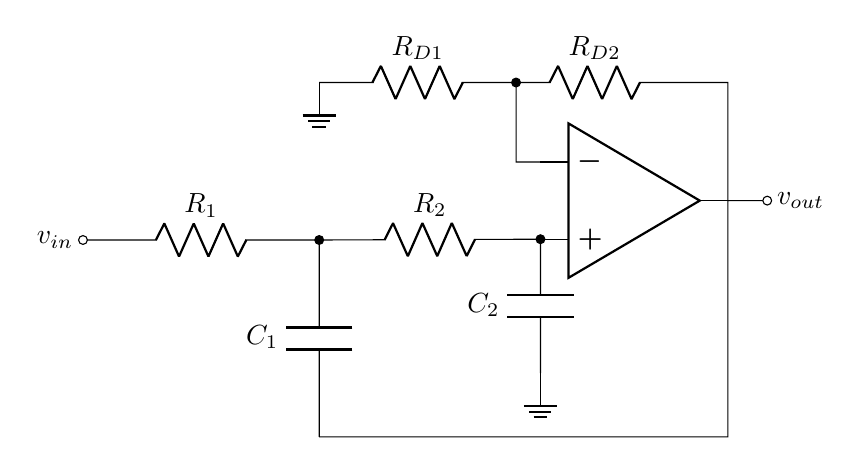
\begin{tikzpicture}
        \draw
        (4,0.5) node [op amp] (opamp) {}
        (-3,0) node [left] {$v_{in}$} to [R, l=$R_1$, o-] (0,0)
        to [R, l=$R_2$] (opamp.+)
        -- (opamp.+) to [C, l_=$C_2$, *-] ($(opamp.+)+(0,-1.7)$) node [ground] {} 
        (opamp.-) -| (2.5,2)
        (2.5,2) to [R, l_=$R_{D1}$, *-] (0, 2) node [ground] {}
        (2.5,2) to [R, l=$R_{D2}$] (4.5,2)
        (opamp.out) |- (4.5, 2)
        (opamp.out) |- (0, -2.5)
        (0, 0) to [C, l_=$C_1$, *-] (0, -2.5)
        (opamp.out) to[short, -o] ($(opamp.out)+(0.5,0)$) node [right] {$v_{out}$}
        ;
    \end{tikzpicture}
    \caption{Implementation of a second-order low-pass filter with a Sallen \&
    Key cell.}
    \label{fig:sallen-key}
\end{figure}

\section{Third-order filters}
Third-order filters can be obtained by adding a $RC$ filter at the output
of a Sallen \& Key cell.

\section{Filter design procedure}
A simplified design procedure could be the following:
\begin{enumerate}
    \item \textbf{Specification}:
        \begin{itemize}
            \item Pattern in the Fourier domain ;
            \item Constraints (number of amplifiers, technology).
        \end{itemize}
    \item \textbf{Approximation}: depending on the pattern specified, choose the type
    of filter (Butterworth, Chebyshev, etc) that fits the best.
    \item \textbf{Factorization}: decompose the transfer function as a product
    of transfer function of order 1 or 2.
    \item \textbf{Realization}:
        \begin{itemize}
            \item Choose a technology ;
            \item Choose an architecture (Sallen \& Key, etc) ;
            \item Compute values of components.
        \end{itemize}
\end{enumerate}

\subsection{Terminology}
A filter is mostly specified by its \emph{passband} and its \emph{stopband}.
In real filters, however, the transition from the passband to the stopband cannot
be infinitely sharp. The steepness of this transition is called the \emph{roll-off}
and is usually measured in \SI{}{\decibel} per decade. 
The \emph{transition band} is defined as the frequency band
where the transition from the passband to the stopband occurs.
In addition, one needs to specify the maximum allowed variation (i.e. ripples)
in the passband, $A_{max}$, and the minimum required stopband attenuation, $A_{min}$.

\section{Reference filters}
\todo[inline]{Group/phase delay of the different filter types.}
The filters presented in this section can be computed easily using the SciPy
Python module or \textsc{Matlab}.

\subsection{Butterworth}
Butterworth filters are characterized by a \textbf{maximally flat 
magnitude within the passband}.
The power transfer function is given by
\[ |H(j\omega)|^2 = \frac{H_0^2}{1+\left(\frac{j\omega}{j\omega_c}\right)^{2n}} \]
where $n$ is the order of the filter, $w_c$ its cutoff frequency (approximately
at -\SI{3}{\decibel}) and $H_0$ its DC gain.
Bode plots for Butterworth filters of orders 1 to 6 are given in
figure~\ref{fig:butterworth}.

\begin{figure}
    \centering
    \resizebox{0.75\textwidth}{!}{% This file was created by matlab2tikz.
%
%The latest updates can be retrieved from
%  http://www.mathworks.com/matlabcentral/fileexchange/22022-matlab2tikz-matlab2tikz
%where you can also make suggestions and rate matlab2tikz.
%
\definecolor{mycolor1}{rgb}{0.75000,0.75000,0.00000}%
\definecolor{mycolor2}{rgb}{0.75000,0.00000,0.75000}%
\definecolor{mycolor3}{rgb}{0.00000,0.75000,0.75000}%
%
\begin{tikzpicture}

\begin{axis}[%
width=5.081in,
height=1.992in,
at={(0.852in,0.269in)},
scale only axis,
separate axis lines,
every outer x axis line/.append style={black},
every x tick label/.append style={font=\color{black}},
xmode=log,
xmin=100000000,
xmax=10000000000,
xminorticks=true,
xmajorgrids,
every outer y axis line/.append style={black},
every y tick label/.append style={font=\color{black}},
ymode=log,
ymin=1e-06,
ymax=10,
yminorticks=true,
ymajorgrids,
axis background/.style={fill=white},
legend style={at={(0.03,0.03)},anchor=south west,legend cell align=left,align=left,draw=black}
]
\addplot [color=blue,solid,line width=2.0pt]
  table[row sep=crcr]{%
100000000	0.995037190209989\\
100462042.134682	0.994991568474029\\
100926219.098705	0.994945530542872\\
101392540.755881	0.994899072678539\\
101861017.015597	0.99485219111056\\
102331657.833024	0.99480488203572\\
102804473.209331	0.994757141617783\\
103279473.191895	0.994708965987239\\
103756667.874518	0.994660351241027\\
104236067.39764	0.994611293442269\\
104717681.948552	0.994561788619999\\
105201521.761616	0.994511832768891\\
105687597.11848	0.994461421848982\\
106175918.3483	0.994410551785398\\
106666495.827954	0.994359218468074\\
107159339.982267	0.994307417751475\\
107654461.284231	0.994255145454314\\
108151870.255229	0.994202397359268\\
108651577.465254	0.994149169212695\\
109153593.533139	0.994095456724343\\
109657929.126781	0.994041255567066\\
110164594.963365	0.993986561376527\\
110673601.809597	0.993931369750913\\
111184960.481927	0.993875676250635\\
111698681.846782	0.993819476398033\\
112214776.820798	0.993762765677082\\
112733256.371048	0.993705539533088\\
113254131.515281	0.993647793372388\\
113777413.322149	0.993589522562046\\
114303112.911448	0.993530722429552\\
114831241.454351	0.99347138826251\\
115361810.173648	0.993411515308331\\
115894830.343981	0.993351098773927\\
116430313.292088	0.99329013382539\\
116968270.397039	0.993228615587687\\
117508713.090481	0.99316653914434\\
118051652.85688	0.993103899537107\\
118597101.233767	0.993040691765668\\
119145069.811978	0.992976910787298\\
119695570.235904	0.992912551516548\\
120248614.203741	0.99284760882492\\
120804213.467733	0.992782077540539\\
121362379.834424	0.992715952447827\\
121923125.164911	0.99264922828717\\
122486461.375093	0.992581899754592\\
123052400.435926	0.992513961501414\\
123620954.373677	0.992445408133927\\
124192135.270178	0.992376234213048\\
124765955.263087	0.992306434253987\\
125342426.54614	0.992236002725904\\
125921561.369415	0.992164934051567\\
126503372.039591	0.99209322260701\\
127087870.920205	0.992020862721185\\
127675070.431926	0.991947848675618\\
128264983.052806	0.991874174704059\\
128857621.318552	0.99179983499213\\
129452997.822791	0.991724823676977\\
130051125.217341	0.991649134846911\\
130652016.212472	0.991572762541059\\
131255683.577185	0.991495700749002\\
131862140.139475	0.991417943410418\\
132471398.786611	0.991339484414723\\
133083472.465408	0.99126031760071\\
133698374.182495	0.991180436756183\\
134316117.004602	0.991099835617594\\
134936714.058831	0.991018507869676\\
135560178.532937	0.990936447145077\\
136186523.675608	0.990853647023989\\
136815762.796747	0.990770101033779\\
137447909.267754	0.990685802648613\\
138082976.521809	0.990600745289087\\
138720978.054162	0.990514922321848\\
139361927.422414	0.990428327059223\\
140005838.24681	0.990340952758833\\
140652724.210524	0.990252792623222\\
141302599.059953	0.990163839799471\\
141955476.60501	0.990074087378818\\
142611370.719413	0.989983528396275\\
143270295.340984	0.989892155830245\\
143932264.47194	0.989799962602131\\
144597292.179202	0.989706941575957\\
145265392.594678	0.989613085557973\\
145936579.915576	0.98951838729627\\
146610868.404698	0.989422839480387\\
147288272.39075	0.989326434740923\\
147968806.26864	0.989229165649139\\
148652484.499786	0.98913102471657\\
149339321.612425	0.989032004394628\\
150029332.201922	0.988932097074206\\
150722530.931076	0.988831295085282\\
151418932.530435	0.988729590696521\\
152118551.798611	0.988626976114878\\
152821403.602586	0.988523443485199\\
153527502.878042	0.988418984889818\\
154236864.629663	0.98831359234816\\
154949503.931463	0.988207257816338\\
155665435.927107	0.988099973186751\\
156384675.830225	0.98799173028768\\
157107238.924745	0.987882520882889\\
157833140.565212	0.987772336671213\\
158562396.177113	0.987661169286163\\
159295021.257212	0.987549010295514\\
160031031.37387	0.987435851200904\\
160770442.167382	0.987321683437425\\
161513269.350309	0.98720649837322\\
162259528.707809	0.987090287309074\\
163009236.097974	0.986973041478009\\
163762407.452169	0.986854752044879\\
164519058.775366	0.986735410105959\\
165279206.14649	0.98661500668854\\
166042865.718753	0.986493532750525\\
166810053.720006	0.986370979180018\\
167580786.453077	0.986247336794919\\
168355080.296121	0.986122596342519\\
169132951.702964	0.985996748499089\\
169914417.203463	0.985869783869481\\
170699493.40384	0.985741692986714\\
171488196.987054	0.985612466311578\\
172280544.71314	0.985482094232221\\
173076553.419573	0.985350567063748\\
173876240.021625	0.985217875047821\\
174679621.512725	0.985084008352248\\
175486714.964815	0.984948957070591\\
176297537.528721	0.984812711221753\\
177112106.434509	0.984675260749591\\
177930438.991858	0.984536595522503\\
178752552.590424	0.984396705333041\\
179578464.70021	0.984255579897506\\
180408192.871939	0.984113208855559\\
181241754.737423	0.983969581769819\\
182079168.009946	0.983824688125475\\
182920450.484629	0.983678517329894\\
183765620.038816	0.983531058712227\\
184614694.632455	0.983382301523025\\
185467692.30847	0.983232234933852\\
186324631.193156	0.983080848036895\\
187185529.496558	0.982928129844588\\
188050405.512858	0.982774069289227\\
188919277.620766	0.982618655222591\\
189792164.28391	0.98246187641557\\
190669084.051225	0.982303721557783\\
191550055.557352	0.982144179257216\\
192435097.523033	0.981983238039844\\
193324228.755504	0.98182088634927\\
194217468.148903	0.981657112546361\\
195114834.684661	0.981491904908882\\
196016347.431918	0.981325251631146\\
196922025.547917	0.981157140823654\\
197831888.278416	0.980987560512744\\
198745954.958099	0.980816498640245\\
199664245.010979	0.98064394306313\\
200586777.950823	0.980469881553176\\
201513573.381556	0.980294301796628\\
202444650.99768	0.980117191393863\\
203380030.584698	0.979938537859062\\
204319732.019527	0.979758328619883\\
205263775.270925	0.979576551017142\\
206212180.399914	0.979393192304494\\
207164967.560208	0.979208239648124\\
208122156.998634	0.979021680126433\\
209083769.055575	0.978833500729745\\
210049824.165391	0.978643688359996\\
211020342.85686	0.978452229830455\\
211995345.753608	0.978259111865425\\
212974853.574552	0.978064321099969\\
213958887.134342	0.977867844079627\\
214947467.343798	0.977669667260149\\
215940615.210357	0.977469777007227\\
216938351.838518	0.977268159596242\\
217940698.430295	0.977064801212\\
218947676.285662	0.976859687948496\\
219959306.803008	0.976652805808668\\
220975611.47959	0.976444140704167\\
221996611.911995	0.976233678455127\\
223022329.796594	0.976021404789945\\
224052786.930002	0.975807305345075\\
225088005.209547	0.975591365664814\\
226128006.633727	0.975373571201112\\
227172813.30269	0.975153907313378\\
228222447.41869	0.974932359268298\\
229276931.286565	0.974708912239665\\
230336287.314214	0.974483551308211\\
231400538.013065	0.974256261461447\\
232469705.998565	0.974027027593523\\
233543813.990648	0.97379583450508\\
234622884.814226	0.973562666903124\\
235706941.399672	0.973327509400906\\
236796006.783308	0.973090346517808\\
237890104.107889	0.972851162679243\\
238989256.623105	0.972609942216561\\
240093487.686065	0.972366669366969\\
241202820.7618	0.972121328273461\\
242317279.42376	0.971873902984753\\
243436887.354311	0.971624377455239\\
244561668.345245	0.971372735544944\\
245691646.298279	0.971118961019504\\
246826845.225569	0.970863037550146\\
247967289.250216	0.97060494871368\\
249113002.60678	0.970344677992515\\
250264009.641791	0.970082208774669\\
251420334.81428	0.969817524353808\\
252582002.696278	0.969550607929284\\
253749037.973357	0.969281442606199\\
254921465.445143	0.969010011395469\\
256099310.025846	0.968736297213914\\
257282596.744793	0.968460282884347\\
258471350.746957	0.968181951135694\\
259665597.293487	0.967901284603114\\
260865361.762255	0.967618265828139\\
262070669.648384	0.967332877258831\\
263281546.564802	0.967045101249946\\
264498018.242773	0.966754920063124\\
265720110.53245	0.966462315867085\\
266947849.403432	0.966167270737844\\
268181260.945302	0.965869766658945\\
269420371.368188	0.965569785521705\\
270665207.003324	0.96526730912548\\
271915794.303601	0.964962319177945\\
273172159.844137	0.964654797295392\\
274434330.322837	0.964344725003041\\
275702332.560958	0.96403208373538\\
276976193.503689	0.963716854836509\\
278255940.220713	0.96339901956051\\
279541599.906785	0.963078559071832\\
280833199.882318	0.962755454445701\\
282130767.593947	0.962429686668542\\
283434330.615131	0.96210123663842\\
284743916.646725	0.961770085165506\\
286059553.517574	0.961436212972561\\
287381269.185107	0.961099600695436\\
288709091.735923	0.960760228883598\\
290043049.386399	0.960418078000673\\
291383170.483279	0.960073128425013\\
292729483.504281	0.95972536045028\\
294082017.058707	0.959374754286054\\
295440799.888038	0.959021290058468\\
296805860.86656	0.958664947810855\\
298177229.001967	0.958305707504422\\
299554933.435981	0.957943549018953\\
300939003.444972	0.957578452153526\\
302329468.440578	0.957210396627256\\
303726357.970331	0.956839362080066\\
305129701.718287	0.956465328073473\\
306539529.505652	0.956088274091412\\
307955871.291422	0.955708179541067\\
309378757.173014	0.955325023753745\\
310808217.386907	0.95493878598576\\
312244282.309286	0.954549445419353\\
313686982.456687	0.954156981163631\\
315136348.486648	0.953761372255538\\
316592411.198352	0.953362597660843\\
318055201.533293	0.952960636275169\\
319524750.575921	0.952555466925034\\
321001089.554317	0.952147068368929\\
322484249.840845	0.95173541929842\\
323974262.95282	0.951320498339276\\
325471160.553184	0.950902284052633\\
326974974.451177	0.950480754936173\\
328485736.603004	0.950055889425348\\
330003479.112529	0.949627665894616\\
331528234.231942	0.94919606265872\\
333060034.36246	0.948761057973991\\
334598912.054998	0.948322630039678\\
336144900.010878	0.947880756999312\\
337698031.08251	0.947435416942101\\
339258338.274099	0.946986587904354\\
340825854.742346	0.94653424787093\\
342400613.797143	0.946078374776733\\
343982648.902292	0.945618946508222\\
345571993.676214	0.945155940904963\\
347168681.892656	0.944689335761211\\
348772747.481417	0.944219108827517\\
350384224.529068	0.943745237812381\\
352003147.279667	0.943267700383925\\
353629550.135505	0.942786474171603\\
355263467.657814	0.942301536767949\\
356904934.567522	0.94181286573035\\
358553985.745982	0.941320438582857\\
360210656.235708	0.940824232818032\\
361874981.241128	0.940324225898822\\
363546996.129332	0.939820395260474\\
365226736.430817	0.939312718312481\\
366914237.840249	0.938801172440561\\
368609536.217217	0.938285735008676\\
370312667.586993	0.937766383361079\\
372023668.141307	0.9372430948244\\
373742574.239106	0.936715846709769\\
375469422.407334	0.93618461631497\\
377204249.341701	0.93564938092663\\
378947091.907467	0.935110117822452\\
380697987.140228	0.934566804273469\\
382456972.246701	0.934019417546351\\
384224084.605506	0.933467934905734\\
385999361.767978	0.93291233361659\\
387782841.458945	0.932352590946638\\
389574561.57755	0.93178868416878\\
391374560.198039	0.931220590563586\\
393182875.570575	0.930648287421806\\
394999546.122066	0.930071752046921\\
396824610.456949	0.929490961757735\\
398658107.358044	0.928905893890994\\
400500075.787362	0.928316525804049\\
402350554.886929	0.927722834877556\\
404209583.97963	0.927124798518206\\
406077202.570037	0.926522394161497\\
407953450.345245	0.925915599274542\\
409838367.175725	0.925304391358909\\
411731993.116168	0.924688747953503\\
413634368.406327	0.924068646637481\\
415545533.471888	0.923444065033202\\
417465528.925313	0.92281498080922\\
419394395.566718	0.9221813716833\\
421332174.384729	0.921543215425485\\
423278906.557354	0.920900489861189\\
425234633.452869	0.920253172874326\\
427199396.630678	0.919601242410482\\
429173237.842215	0.918944676480109\\
431156199.031823	0.918283453161768\\
433148322.337639	0.9176175506054\\
435149650.092505	0.916946947035628\\
437160224.82485	0.916271620755104\\
439180089.259608	0.915591550147879\\
441209286.319119	0.914906713682812\\
443247859.124041	0.914217089917015\\
445295850.994266	0.913522657499326\\
447353305.449846	0.912823395173819\\
449420266.211913	0.912119281783342\\
451496777.20361	0.911410296273096\\
453582882.551018	0.910696417694234\\
455678626.584105	0.909977625207502\\
457784053.837662	0.909253898086902\\
459899209.052245	0.908525215723396\\
462024137.175131	0.907791557628632\\
464158883.361279	0.907052903438698\\
466303492.974272	0.906309232917921\\
468458011.587305	0.905560525962666\\
470622484.984127	0.904806762605199\\
472796959.160039	0.904047923017544\\
474981480.322851	0.903283987515393\\
477176094.893875	0.902514936562026\\
479380849.508911	0.901740750772263\\
481595791.019234	0.900961410916445\\
483820966.492596	0.900176897924429\\
486056423.214215	0.899387192889623\\
488302208.687788	0.898592277073029\\
490558370.636505	0.897792131907314\\
492824957.00405	0.896986739000907\\
495102015.955635	0.896176080142115\\
497389595.879008	0.895360137303253\\
499687745.385489	0.894538892644809\\
501996513.311008	0.893712328519604\\
504315948.717137	0.892880427476997\\
506646100.892127	0.89204317226709\\
508987019.351967	0.891200545844948\\
511338753.841433	0.890352531374849\\
513701354.335134	0.889499112234536\\
516074871.038592	0.888640272019484\\
518459354.389291	0.887775994547187\\
520854855.057765	0.886906263861446\\
523261423.948667	0.88603106423668\\
525679112.201842	0.885150380182235\\
528107971.193432	0.884264196446713\\
530548052.536957	0.883372498022293\\
532999408.084408	0.882475270149083\\
535462089.927361	0.881572498319449\\
537936150.39807	0.880664168282373\\
540421642.07059	0.879750266047796\\
542918617.761894	0.878830777890977\\
545427130.532982	0.877905690356846\\
547947233.690029	0.876974990264356\\
550478980.785497	0.876038664710839\\
553022425.619291	0.875096701076353\\
555577622.239888	0.874149087028033\\
558144624.945495	0.873195810524428\\
560723488.285204	0.872236859819839\\
563314267.060135	0.871272223468649\\
565917016.324625	0.870301890329636\\
568531791.387375	0.869325849570291\\
571158647.812642	0.868344090671107\\
573797641.421412	0.867356603429869\\
576448828.292587	0.866363377965922\\
579112264.764177	0.865364404724428\\
581788007.434494	0.864359674480607\\
584476113.163363	0.863349178343949\\
587176639.073326	0.862332907762422\\
589889642.550849	0.861310854526649\\
592615181.247556	0.860283010774062\\
595353313.081439	0.859249368993038\\
598104096.238093	0.85820992202701\\
600867589.171969	0.857164663078532\\
603643850.607586	0.856113585713351\\
606432939.540807	0.855056683864415\\
609234915.240071	0.85399395183587\\
612049837.247669	0.852925384307014\\
614877765.381003	0.851850976336224\\
617718759.733849	0.850770723364842\\
620572880.677649	0.849684621221023\\
623440188.862786	0.848592666123547\\
626320745.219868	0.847494854685595\\
629214610.961035	0.846391183918467\\
632121847.581245	0.845281651235279\\
635042516.859595	0.84416625445459\\
637976680.860628	0.843044991804005\\
640924401.935647	0.841917861923717\\
643885742.724043	0.840784863870002\\
646860766.154632	0.839645997118661\\
649849535.446988	0.838501261568413\\
652852114.112785	0.83735065754423\\
655868565.957145	0.836194185800622\\
658898955.079996	0.835031847524856\\
661943345.877439	0.833863644340119\\
665001803.04311	0.832689578308626\\
668074391.569561	0.831509651934658\\
671161176.749627	0.830323868167543\\
674262224.177835	0.829132230404567\\
677377599.751775	0.827934742493823\\
680507369.673522	0.826731408736983\\
683651600.451024	0.825522233892017\\
686810358.899529	0.824307223175822\\
689983712.143003	0.823086382266789\\
693171727.61554	0.821859717307304\\
696374473.062824	0.820627234906149\\
699592016.543537	0.819388942140855\\
702824426.430837	0.818144846559956\\
706071771.413778	0.816894956185175\\
709334120.498799	0.815639279513525\\
712611543.011173	0.814377825519324\\
715904108.596489	0.813110603656136\\
719211887.222121	0.811837623858622\\
722534949.178722	0.810558896544304\\
725873365.081725	0.809274432615239\\
729227205.872833	0.807984243459613\\
732596542.821523	0.806688340953241\\
735981447.526579	0.805386737460971\\
739381991.917587	0.80407944583801\\
742798248.256491	0.802766479431136\\
746230289.139112	0.801447852079834\\
749678187.496688	0.800123578117332\\
753142016.597436	0.798793672371534\\
756621850.048106	0.797458150165862\\
760117761.795532	0.796117027320002\\
763629826.128223	0.794770320150541\\
767158117.67793	0.793418045471511\\
770702711.421229	0.792060220594837\\
774263682.681128	0.790696863330667\\
777841107.128648	0.78932799198762\\
781435060.784453	0.787953625372908\\
785045620.020451	0.786573782792374\\
788672861.561417	0.785188484050415\\
792316862.486626	0.783797749449802\\
795977700.231498	0.782401599791388\\
799655452.589233	0.781000056373718\\
803350197.712477	0.779593140992528\\
807062014.114952	0.778180875940141\\
810790980.673169	0.776763284004739\\
814537176.628074	0.775340388469545\\
818300681.586741	0.773912213111887\\
822081575.524054	0.772478782202156\\
825879938.784429	0.771040120502649\\
829695852.083492	0.769596253266307\\
833529396.509819	0.768147206235344\\
837380653.526647	0.766693005639758\\
841249704.973608	0.765233678195743\\
845136633.068474	0.763769251103976\\
849041520.408875	0.762299752047821\\
852964449.974102	0.76082520919138\\
856905505.126833	0.759345651177473\\
860864769.614924	0.757861107125485\\
864842327.573174	0.756371606629121\\
868838263.525119	0.754877179754028\\
872852662.384837	0.753377857035329\\
876885609.458741	0.751873669475034\\
880937190.447396	0.750364648539349\\
885007491.447346	0.748850826155874\\
889096598.952917	0.747332234710702\\
893204599.858096	0.745808907045386\\
897331581.45835	0.744280876453827\\
901477631.452492	0.742748176679042\\
905642837.944528	0.741210841909827\\
909827289.445557	0.739668906777315\\
914031074.875622	0.738122406351436\\
918254283.56563	0.736571376137259\\
922497005.259218	0.735015852071253\\
926759330.114686	0.73345587051742\\
931041348.706908	0.731891468263351\\
935343152.029238	0.730322682516172\\
939664831.495467	0.728749550898383\\
944006478.94176	0.727172111443612\\
948368186.628595	0.72559040259227\\
952750047.24273	0.724004463187105\\
957152153.899186	0.72241433246866\\
961574600.143208	0.720820050070648\\
966017479.952268	0.719221656015221\\
970480887.738033	0.717619190708172\\
974964918.34841	0.716012694934013\\
979469667.069539	0.714402209850991\\
983995229.627821	0.712787776986014\\
988541702.191957	0.711169438229482\\
993109181.374978	0.709547235830046\\
997697764.236321	0.707921212389273\\
1002307548.28386	0.706291410856243\\
1006938631.47603	0.704657874522056\\
1011591112.22383	0.70302064701427\\
1016265089.393	0.701379772291257\\
1020960662.30605	0.699735294636493\\
1025677930.74442	0.698087258652765\\
1030416994.95059	0.696435709256316\\
1035177955.63017	0.694780691670921\\
1039960913.95412	0.69312225142189\\
1044765971.56081	0.69146043433002\\
1049593230.55823	0.689795286505462\\
1054442793.52617	0.688126854341542\\
1059314763.51837	0.686455184508528\\
1064209244.06473	0.684780323947326\\
1069126339.17348	0.683102319863125\\
1074066153.33343	0.68142121971899\\
1079028791.51619	0.679737071229408\\
1084014359.17833	0.678049922353783\\
1089022962.26373	0.676359821289868\\
1094054707.20574	0.674666816467184\\
1099109700.9295	0.672970956540363\\
1104188050.85416	0.671272290382468\\
1109289864.89522	0.66957086707828\\
1114415251.46679	0.66786673591752\\
1119564319.48388	0.666159946388078\\
1124737178.36475	0.664450548169168\\
1129933938.03322	0.662738591124483\\
1135154708.921	0.661024125295302\\
1140399601.97004	0.659307200893595\\
1145668728.63487	0.65758786829507\\
1150962200.88503	0.655866178032229\\
1156280131.20737	0.65414218078739\\
1161622632.6085	0.652415927385693\\
1166989818.61715	0.650687468788096\\
1172381803.2866	0.648956856084357\\
1177798701.19712	0.647224140485991\\
1183240627.45838	0.645489373319244\\
1188707697.71191	0.643752606018038\\
1194200028.13353	0.64201389011693\\
1199717735.43589	0.64027327724405\\
1205260936.87084	0.638530819114052\\
1210829750.23204	0.636786567521066\\
1216424293.85737	0.635040574331651\\
1222044686.63149	0.633292891477758\\
1227691047.98836	0.631543570949697\\
1233363497.91377	0.629792664789114\\
1239062156.94791	0.628040225081988\\
1244787146.1879	0.626286303951638\\
1250538587.29039	0.624530953551742\\
1256316602.47412	0.622774226059394\\
1262121314.52255	0.621016173668146\\
1267952846.78643	0.619256848581112\\
1273811323.18647	0.617496303004072\\
1279696868.21594	0.615734589138608\\
1285609606.9433	0.613971759175283\\
1291549665.01488	0.612207865286819\\
1297517168.65758	0.610442959621339\\
1303512244.68151	0.608677094295627\\
1309535020.48267	0.606910321388429\\
1315585624.04571	0.605142692933793\\
1321664183.9466	0.603374260914435\\
1327770829.35543	0.601605077255169\\
1333905690.03906	0.599835193816366\\
1340068896.36395	0.598064662387455\\
1346260579.29891	0.596293534680479\\
1352480870.41787	0.594521862323698\\
1358729901.90271	0.592749696855233\\
1365007806.54601	0.590977089716774\\
1371314717.75394	0.589204092247328\\
1377650769.54906	0.587430755677027\\
1384016096.57313	0.585657131121\\
1390410834.09007	0.583883269573282\\
1396835117.98874	0.582109221900799\\
1403289084.78588	0.580335038837409\\
1409772871.62897	0.578560770978\\
1416286616.2992	0.576786468772647\\
1422830457.21435	0.575012182520846\\
1429404533.43176	0.573237962365797\\
1436008984.65126	0.571463858288771\\
1442643951.21816	0.569689920103523\\
1449309574.12621	0.567916197450794\\
1456005995.02065	0.566142739792862\\
1462733356.20113	0.564369596408182\\
1469491800.62482	0.562596816386088\\
1476281471.90939	0.560824448621569\\
1483102514.3361	0.559052541810113\\
1489955072.85286	0.557281144442631\\
1496839293.07726	0.555510304800464\\
1503755321.29974	0.553740070950444\\
1510703304.48666	0.551970490740053\\
1517683390.2834	0.550201611792646\\
1524695727.01757	0.548433481502757\\
1531740463.70208	0.546666147031481\\
1538817750.03835	0.544899655301946\\
1545927736.41948	0.543134052994847\\
1553070573.93346	0.541369386544069\\
1560246414.36636	0.539605702132397\\
1567455410.2056	0.537843045687295\\
1574697714.64309	0.53608146287678\\
1581973481.5786	0.53432099910537\\
1589282865.62298	0.532561699510108\\
1596626022.10143	0.530803608956686\\
1604003107.05682	0.52904677203564\\
1611414277.25302	0.527291233058629\\
1618859690.1782	0.5255370360548\\
1626339504.04819	0.523784224767243\\
1633853877.80986	0.522032842649514\\
1641402971.14447	0.520282932862259\\
1648986944.47106	0.518534538269912\\
1656605958.94992	0.516787701437475\\
1664260176.4859	0.515042464627401\\
1671949759.73199	0.513298869796531\\
1679674872.09265	0.51155695859314\\
1687435677.72737	0.509816772354064\\
1695232341.55412	0.508078352101891\\
1703065029.25284	0.506341738542267\\
1710933907.26902	0.504606972061254\\
1718839142.81715	0.5028740927228\\
1726780903.88435	0.501143140266267\\
1734759359.23393	0.499414154104064\\
1742774678.40892	0.497687173319347\\
1750827031.73573	0.495962236663808\\
1758916590.32773	0.49423938255555\\
1767043526.08894	0.492518649077029\\
1775208011.71764	0.490800073973096\\
1783410220.71001	0.489083694649113\\
1791650327.3639	0.487369548169135\\
1799928506.78248	0.485657671254204\\
1808244934.87795	0.483948100280685\\
1816599788.37533	0.48224087127871\\
1824993244.81615	0.480536019930694\\
1833425482.56229	0.478833581569912\\
1841896680.79971	0.47713359117918\\
1850407019.54231	0.475436083389589\\
1858956679.63569	0.473741092479338\\
1867545842.76107	0.472048652372618\\
1876174691.43912	0.47035879663859\\
1884843409.0338	0.468671558490435\\
1893552179.7563	0.466986970784464\\
1902301188.66895	0.46530506601932\\
1911090621.68914	0.463625876335238\\
1919920665.59329	0.461949433513378\\
1928791508.02078	0.460275768975245\\
1937703337.47799	0.458604913782153\\
1946656343.34226	0.456936898634781\\
1955650715.86595	0.455271753872781\\
1964686646.18045	0.453609509474467\\
1973764326.30026	0.451950195056565\\
1982883949.12707	0.450293839874025\\
1992045708.45387	0.448640472819903\\
2001249798.96903	0.446990122425316\\
2010496416.2605	0.445342816859437\\
2019785756.81989	0.443698583929578\\
2029118018.04668	0.442057451081325\\
2038493398.25246	0.440419445398725\\
2047912096.66508	0.438784593604549\\
2057374313.43291	0.437152922060603\\
2066880249.62908	0.435524456768104\\
2076430107.25577	0.433899223368112\\
2086024089.2485	0.43227724714201\\
2095662399.48043	0.430658553012061\\
2105345242.76671	0.429043165541988\\
2115072824.86879	0.427431108937644\\
2124845352.49889	0.425822407047702\\
2134663033.32425	0.424217083364424\\
2144526075.97167	0.422615161024459\\
2154434690.03188	0.421016662809712\\
2164389086.06402	0.419421611148237\\
2174389475.60008	0.417830028115208\\
2184436071.14943	0.416241935433918\\
2194529086.20332	0.41465735447682\\
2204668735.23941	0.413076306266637\\
2214855233.72636	0.41149881147749\\
2225088798.12837	0.409924890436089\\
2235369645.9098	0.408354563122959\\
2245697995.53977	0.406787849173706\\
2256074066.49686	0.405224767880326\\
2266498079.27369	0.403665338192564\\
2276970255.38168	0.402109578719288\\
2287490817.3557	0.400557507729931\\
2298059988.75885	0.399009143155945\\
2308677994.18717	0.397464502592303\\
2319345059.27443	0.395923603299045\\
2330061410.69693	0.394386462202835\\
2340827276.17829	0.392853095898579\\
2351642884.49435	0.391323520651053\\
2362508465.47795	0.389797752396576\\
2373424250.02387	0.388275806744714\\
2384390470.09373	0.386757698980004\\
2395407358.72088	0.385243444063724\\
2406475150.01542	0.383733056635671\\
2417594079.16913	0.382226551015984\\
2428764382.46045	0.38072394120699\\
2439986297.25956	0.379225240895063\\
2451260062.03334	0.377730463452534\\
2462585916.35054	0.376239621939594\\
2473964100.88682	0.374752729106242\\
2485394857.42981	0.373269797394258\\
2496878428.88433	0.371790838939181\\
2508415059.27754	0.370315865572316\\
2520004993.76409	0.368844888822768\\
2531648478.63135	0.367377919919488\\
2543345761.30466	0.365914969793337\\
2555097090.3525	0.364456049079182\\
2566902715.49195	0.363001168117975\\
2578762887.5938	0.361550336958898\\
2590677858.688	0.360103565361479\\
2602647881.969	0.358660862797748\\
2614673211.8011	0.357222238454403\\
2626754103.72384	0.355787701234985\\
2638890814.45751	0.354357259762067\\
2651083601.90853	0.352930922379457\\
2663332725.17498	0.351508697154413\\
2675638444.55205	0.350090591879873\\
2688001021.53761	0.348676614076684\\
2700420718.83777	0.347266770995848\\
2712897800.37247	0.345861069620777\\
2725432531.28103	0.344459516669561\\
2738025177.92786	0.343062118597227\\
2750676007.90807	0.341668881598027\\
2763385290.05317	0.340279811607715\\
2776153294.43679	0.33889491430584\\
2788980292.38044	0.337514195118039\\
2801866556.4592	0.336137659218341\\
2814812360.50758	0.334765311531469\\
2827817979.62534	0.333397156735143\\
2840883690.18331	0.332033199262396\\
2854009769.82924	0.330673443303892\\
2867196497.49376	0.329317892810229\\
2880444153.3963	0.327966551494268\\
2893753019.05095	0.326619422833446\\
2907123377.27258	0.325276510072093\\
2920555512.18274	0.323937816223756\\
2934049709.21578	0.322603344073513\\
2947606255.12486	0.32127309618029\\
2961225437.98803	0.319947074879184\\
2974907547.21444	0.318625282283767\\
2988652873.55038	0.31730772028841\\
3002461709.08554	0.315994390570581\\
3016334347.2592	0.314685294593158\\
3030271082.86639	0.313380433606733\\
3044272212.06431	0.312079808651908\\
3058338032.37843	0.310783420561591\\
3072468842.70901	0.309491269963284\\
3086664943.33727	0.308203357281376\\
3100926635.93194	0.306919682739411\\
3115254223.55548	0.305640246362376\\
3129648010.67075	0.304365047978952\\
3144108303.14726	0.303094087223794\\
3158635408.26782	0.301827363539771\\
3173229634.73497	0.300564876180225\\
3187891292.67765	0.299306624211202\\
3202620693.65765	0.298052606513693\\
3217418150.67636	0.296802821785851\\
3232283978.18138	0.295557268545213\\
3247218492.07313	0.294315945130909\\
3262222009.71166	0.293078849705854\\
3277294849.92338	0.291845980258943\\
3292437333.00778	0.290617334607233\\
3307649780.74424	0.289392910398113\\
3322932516.39897	0.288172705111461\\
3338285864.73176	0.2869567160618\\
3353710152.00293	0.285744940400438\\
3369205705.98027	0.284537375117596\\
3384772855.94598	0.283334017044532\\
3400411932.7037	0.282134862855644\\
3416123268.58553	0.280939909070571\\
3431907197.45904	0.279749152056281\\
3447764054.73447	0.278562588029139\\
3463694177.37173	0.277380213056982\\
3479697903.88769	0.276202023061154\\
3495775574.36328	0.275028013818558\\
3511927530.45073	0.27385818096368\\
3528154115.38088	0.272692519990601\\
3544455673.97044	0.271531026254998\\
3560832552.62927	0.270373694976141\\
3577285099.36788	0.269220521238861\\
3593813663.80464	0.268071499995521\\
3610418597.17333	0.266926626067964\\
3627100252.33065	0.265785894149445\\
3643858983.76354	0.26464929880657\\
3660695147.59689	0.263516834481192\\
3677609101.60105	0.262388495492316\\
3694601205.19931	0.261264276037989\\
3711671819.47577	0.26014417019716\\
3728821307.18283	0.25902817193154\\
3746050032.74898	0.257916275087452\\
3763358362.28653	0.25680847339765\\
3780746663.59934	0.255704760483146\\
3798215306.19074	0.254605129855001\\
3815764661.27126	0.25350957491612\\
3833395101.76661	0.252418088963023\\
3851107002.32557	0.251330665187601\\
3868900739.32798	0.250247296678866\\
3886776690.89267	0.249167976424682\\
3904735236.88556	0.248092697313476\\
3922776758.92771	0.247021452135948\\
3940901640.40345	0.245954233586751\\
3959110266.46847	0.244891034266172\\
3977403024.05804	0.24383184668179\\
3995780301.89527	0.242776663250115\\
4014242490.49931	0.241725476298224\\
4032789982.19371	0.240678278065376\\
4051423171.11466	0.239635060704615\\
4070142453.21944	0.238595816284356\\
4088948226.29486	0.237560536789956\\
4107840889.96565	0.236529214125273\\
4126820845.70295	0.235501840114217\\
4145888496.83292	0.234478406502267\\
4165044248.54519	0.233458904957999\\
4184288507.90158	0.232443327074577\\
4203621683.84472	0.231431664371246\\
4223044187.20667	0.230423908294802\\
4242556430.71779	0.229420050221048\\
4262158829.01533	0.228420081456243\\
4281851798.65241	0.227423993238522\\
4301635758.1068	0.226431776739322\\
4321511127.78976	0.225443423064777\\
4341478330.05508	0.224458923257103\\
4361537789.20801	0.223478268295976\\
4381689931.51419	0.222501449099889\\
4401935185.20888	0.221528456527491\\
4422273980.5059	0.220559281378928\\
4442706749.60689	0.21959391439715\\
4463233926.7104	0.218632346269219\\
4483855948.02118	0.217674567627598\\
4504573251.75944	0.216720569051423\\
4525386278.17017	0.215770341067766\\
4546295469.53241	0.214823874152887\\
4567301270.16875	0.21388115873346\\
4588404126.45475	0.212942185187801\\
4609604486.82842	0.212006943847071\\
4630902801.79976	0.21107542499647\\
4652299523.96018	0.210147618876423\\
4673795107.99246	0.209223515683735\\
4695390010.68007	0.208303105572759\\
4717084690.91702	0.207386378656527\\
4738879609.71765	0.206473325007881\\
4760775230.22638	0.205563934660587\\
4782772017.72749	0.204658197610438\\
4804870439.65514	0.203756103816339\\
4827070965.60317	0.202857643201391\\
4849374067.33523	0.201962805653942\\
4871780218.79464	0.20107158102865\\
4894289896.11453	0.200183959147514\\
4916903577.62802	0.199299929800901\\
4939621743.87833	0.198419482748557\\
4962444877.62891	0.197542607720616\\
4985373463.8739	0.196669294418577\\
5008407989.84821	0.19579953251629\\
5031548945.03805	0.194933311660914\\
5054796821.19125	0.194070621473873\\
5078152112.32765	0.193211451551798\\
5101615314.74982	0.192355791467446\\
5125186927.05335	0.191503630770629\\
5148867450.13749	0.190654958989117\\
5172657387.21602	0.189809765629518\\
5196557243.82766	0.188968040178181\\
5220567527.84696	0.188129772102051\\
5244688749.49514	0.187294950849532\\
5268921421.35067	0.186463565851343\\
5293266058.36055	0.185635606521342\\
5317723177.85094	0.184811062257362\\
5342293299.53836	0.18398992244202\\
5366976945.54048	0.183172176443529\\
5391774640.38749	0.182357813616481\\
5416686911.03316	0.181546823302634\\
5441714286.86589	0.180739194831687\\
5466857299.72017	0.179934917522037\\
5492116483.88779	0.179133980681531\\
5517492376.12914	0.17833637360821\\
5542985515.68467	0.177542085591036\\
5568596444.28641	0.176751105910609\\
5594325706.16937	0.175963423839884\\
5620173848.08319	0.175179028644868\\
5646141419.30368	0.174397909585309\\
5672228971.64455	0.173620055915378\\
5698437059.46916	0.172845456884338\\
5724766239.70217	0.172074101737209\\
5751217071.84159	0.171305979715411\\
5777790117.97052	0.170541080057414\\
5804485942.76898	0.169779391999372\\
5831305113.52622	0.169020904775736\\
5858248200.15255	0.168265607619876\\
5885315775.19145	0.167513489764686\\
5912508413.83189	0.166764540443176\\
5939826693.92036	0.166018748889063\\
5967271195.97331	0.165276104337345\\
5994842503.18942	0.164536596024873\\
6022541201.46193	0.163800213190914\\
6050367879.39121	0.163066945077696\\
6078323128.29724	0.162336780930957\\
6106407542.23204	0.161609710000483\\
6134621717.99249	0.160885721540625\\
6162966255.13294	0.160164804810826\\
6191441755.97783	0.15944694907613\\
6220048825.63472	0.158732143607679\\
6248788072.00689	0.158020377683216\\
6277660105.80651	0.157311640587563\\
6306665540.56741	0.156605921613104\\
6335804992.65827	0.155903210060255\\
6365079081.29558	0.155203495237927\\
6394488428.55696	0.154506766463981\\
6424033659.3942	0.153813013065677\\
6453715401.6467	0.153122224380113\\
6483534286.05471	0.152434389754659\\
6513490946.27281	0.151749498547383\\
6543586018.88326	0.15106754012747\\
6573820143.40957	0.150388503875635\\
6604193962.33031	0.149712379184521\\
6634708121.09234	0.149039155459107\\
6665363268.12489	0.14836882211709\\
6696160054.85324	0.14770136858927\\
6727099135.71232	0.147036784319937\\
6758181168.16111	0.146375058767225\\
6789406812.69613	0.14571618140349\\
6820776732.86569	0.145060141715662\\
6852291595.28409	0.144406929205593\\
6883952069.64551	0.143756533390409\\
6915758828.73853	0.143108943802843\\
6947712548.46023	0.142464149991567\\
6979813907.83067	0.141822141521522\\
7012063589.00721	0.141182907974233\\
7044462277.29905	0.14054643894813\\
7077010661.18189	0.139912724058849\\
7109709432.31245	0.139281752939535\\
7142559285.5431	0.138653515241145\\
7175560918.93692	0.138028000632731\\
7208715033.78215	0.137405198801729\\
7242022334.60732	0.13678509945424\\
7275483529.19625	0.136167692315298\\
7309099328.60295	0.135552967129146\\
7342870447.16676	0.134940913659495\\
7376797602.52775	0.134331521689781\\
7410881515.6416	0.133724781023419\\
7445122910.79516	0.133120681484054\\
7479522515.62183	0.132519212915797\\
7514081061.11696	0.131920365183465\\
7548799281.65342	0.131324128172817\\
7583677914.99716	0.130730491790775\\
7618717702.32298	0.13013944596565\\
7653919388.23016	0.12955098064736\\
7689283720.75827	0.128965085807644\\
7724811451.40342	0.128381751440264\\
7760503335.13357	0.127800967561218\\
7796360130.40525	0.127222724208932\\
7832382599.17917	0.126647011444458\\
7868571506.93688	0.126073819351661\\
7904927622.6964	0.125503138037411\\
7941451719.02934	0.124934957631756\\
7978144572.07661	0.124369268288107\\
8015006961.56541	0.123806060183406\\
8052039670.8255	0.123245323518297\\
8089243486.80595	0.122687048517289\\
8126619200.09195	0.122131225428919\\
8164167604.92146	0.121577844525908\\
8201889499.20218	0.121026896105309\\
8239785684.52855	0.120478370488665\\
8277856966.19845	0.119932258022147\\
8316104153.23096	0.119388549076695\\
8354528058.38289	0.11884723404816\\
8393129498.16637	0.118308303357434\\
8431909292.86625	0.117771747450583\\
8470868266.55742	0.117237556798969\\
8510007247.12225	0.116705721899378\\
8549327066.2684	0.116176233274137\\
8588828559.54626	0.11564908147123\\
8628512566.36692	0.115124257064411\\
8668379930.01979	0.114601750653315\\
8708431497.69069	0.114081552863562\\
8748668120.4799	0.113563654346858\\
8789090653.41993	0.113048045781099\\
8829699955.49408	0.112534717870465\\
8870496889.65442	0.112023661345515\\
8911482322.8402	0.111514866963273\\
8952657125.99638	0.11100832550732\\
8994022174.09205	0.110504027787875\\
9035578346.13892	0.11000196464188\\
9077326525.21021	0.109502126933074\\
9119267598.45934	0.109004505552069\\
9161402457.1385	0.108509091416429\\
9203731996.61823	0.108015875470731\\
9246257116.40573	0.107524848686637\\
9288978720.16452	0.107036002062959\\
9331897715.73324	0.10654932662572\\
9375015015.14531	0.106064813428212\\
9418331534.64796	0.105582453551054\\
9461848194.72199	0.105102238102246\\
9505565920.10117	0.104624158217221\\
9549485639.79197	0.104148205058892\\
9593608287.09313	0.103674369817703\\
9637934799.6158	0.103202643711667\\
9682466119.30311	0.102733017986417\\
9727203192.45052	0.102265483915236\\
9772146969.72573	0.101800032799102\\
9817298406.18886	0.101336655966717\\
9862658461.31283	0.100875344774547\\
9908228099.00379	0.100416090606847\\
9954008287.6215	0.0999588848756908\\
10000000000	0.0995037190209989\\
};
\addlegendentry{n = 1};

\addplot [color=mycolor1,solid,line width=2.0pt]
  table[row sep=crcr]{%
100000000	0.999950003749688\\
100461081.093309	0.99994907533056\\
100924288.144363	0.999948129672239\\
101389630.955553	0.999947166454673\\
101857119.374465	0.999946185351868\\
102326763.294089	0.999945186031781\\
102798572.653033	0.999944168156208\\
103272557.435726	0.999943131380666\\
103748727.672639	0.999942075354279\\
104227093.440486	0.999940999719662\\
104707664.862445	0.999939904112794\\
105190452.10837	0.9999387881629\\
105675465.395008	0.999937651492326\\
106162714.98621	0.999936493716408\\
106652211.193154	0.999935314443343\\
107143964.374561	0.999934113274059\\
107637984.936913	0.999932889802077\\
108134283.334676	0.999931643613377\\
108632870.070517	0.999930374286254\\
109133755.69553	0.999929081391182\\
109636950.80946	0.99992776449066\\
110142466.060922	0.999926423139072\\
110650312.147633	0.999925056882533\\
111160499.816633	0.999923665258737\\
111673039.864515	0.999922247796799\\
112187943.137653	0.999920804017097\\
112705220.532432	0.999919333431113\\
113224882.995479	0.999917835541261\\
113746941.523892	0.999916309840727\\
114271407.165476	0.999914755813292\\
114798291.018973	0.999913172933161\\
115327604.234303	0.999911560664784\\
115859358.012793	0.999909918462677\\
116393563.607418	0.999908245771234\\
116930232.32304	0.999906542024544\\
117469375.516644	0.999904806646197\\
118011004.597579	0.999903039049092\\
118555131.027801	0.999901238635234\\
119101766.322118	0.999899404795541\\
119650922.048426	0.999897536909627\\
120202609.82796	0.999895634345604\\
120756841.33554	0.999893696459861\\
121313628.299814	0.999891722596849\\
121872982.503512	0.999889712088862\\
122434915.783687	0.999887664255809\\
122999440.031973	0.999885578404986\\
123566567.194836	0.999883453830844\\
124136309.273822	0.999881289814746\\
124708678.325815	0.99987908562473\\
125283686.46329	0.99987684051526\\
125861345.854572	0.999874553726974\\
126441668.724092	0.99987222448643\\
127024667.352642	0.999869852005842\\
127610354.077643	0.99986743548282\\
128198741.293399	0.999864974100092\\
128789841.451362	0.999862467025236\\
129383667.060397	0.999859913410394\\
129980230.687042	0.99985731239199\\
130579544.955778	0.999854663090436\\
131181622.549298	0.999851964609841\\
131786476.208768	0.999849216037699\\
132394118.734104	0.999846416444595\\
133004562.98424	0.99984356488388\\
133617821.877398	0.999840660391361\\
134233908.391365	0.99983770198497\\
134852835.563766	0.999834688664437\\
135474616.492342	0.999831619410953\\
136099264.33522	0.999828493186825\\
136726792.311201	0.99982530893513\\
137357213.700035	0.999822065579356\\
137990541.842702	0.999818762023041\\
138626790.141693	0.999815397149407\\
139265972.061296	0.999811969820977\\
139908101.127883	0.999808478879201\\
140553190.930191	0.99980492314406\\
141201255.119612	0.999801301413674\\
141852307.410483	0.999797612463891\\
142506361.580374	0.999793855047886\\
143163431.470383	0.999790027895729\\
143823530.985425	0.999786129713971\\
144486674.094528	0.999782159185198\\
145152874.831128	0.999778114967597\\
145822147.293368	0.999773995694501\\
146494505.644394	0.999769799973929\\
147169964.112657	0.999765526388122\\
147848536.992209	0.999761173493064\\
148530238.643014	0.999756739817997\\
149215083.491243	0.999752223864932\\
149903086.029585	0.999747624108138\\
150594260.817554	0.999742938993637\\
151288622.481791	0.999738166938681\\
151986185.716381	0.999733306331217\\
152686965.28316	0.999728355529351\\
153390976.012028	0.999723312860797\\
154098232.801261	0.999718176622313\\
154808750.617829	0.999712945079131\\
155522544.497715	0.999707616464378\\
156239629.546227	0.999702188978483\\
156960020.93832	0.999696660788571\\
157683733.91892	0.999691030027852\\
158410783.803243	0.999685294794997\\
159141185.977121	0.999679453153495\\
159874955.897328	0.999673503131014\\
160612109.091906	0.99966744271873\\
161352661.160493	0.999661269870666\\
162096627.774655	0.999654982502999\\
162844024.678214	0.999648578493365\\
163594867.687588	0.999642055680152\\
164349172.692119	0.999635411861774\\
165106955.654411	0.999628644795938\\
165868232.610671	0.999621752198891\\
166633019.671044	0.999614731744659\\
167401333.019957	0.999607581064272\\
168173188.916458	0.999600297744969\\
168948603.694565	0.999592879329394\\
169727593.763611	0.999585323314778\\
170510175.608581	0.999577627152101\\
171296365.79048	0.999569788245242\\
172086180.946664	0.999561803950114\\
172879637.791206	0.999553671573783\\
173676753.115242	0.99954538837357\\
174477543.787328	0.999536951556135\\
175282026.7538	0.999528358276551\\
176090219.03913	0.99951960563735\\
176902137.746285	0.999510690687567\\
177717800.057092	0.999501610421748\\
178537223.232599	0.999492361778961\\
179360424.613442	0.999482941641768\\
180187421.620213	0.999473346835195\\
181018231.753824	0.999463574125674\\
181852872.595882	0.999453620219968\\
182691361.80906	0.999443481764081\\
183533717.13747	0.99943315534214\\
184379956.407037	0.999422637475264\\
185230097.525881	0.999411924620411\\
186084158.484689	0.999401013169196\\
186942157.357105	0.999389899446706\\
187804112.300101	0.999378579710273\\
188670041.554374	0.999367050148237\\
189539963.444717	0.999355306878687\\
190413896.380425	0.999343345948171\\
191291858.855667	0.999331163330392\\
192173869.449889	0.999318754924877\\
193059946.828202	0.999306116555616\\
193950109.741779	0.999293243969691\\
194844377.028249	0.999280132835864\\
195742767.612101	0.999266778743152\\
196645300.50508	0.999253177199369\\
197551994.806589	0.999239323629647\\
198462869.704094	0.999225213374925\\
199377944.473538	0.999210841690418\\
200297238.479732	0.999196203744053\\
201220771.176781	0.999181294614879\\
202148562.108487	0.999166109291446\\
203080630.908765	0.999150642670162\\
204016997.302057	0.999134889553615\\
204957681.103752	0.999118844648864\\
205902702.220606	0.999102502565704\\
206852080.651156	0.999085857814898\\
207805836.486153	0.999068904806379\\
208763989.908984	0.999051637847414\\
209726561.19609	0.999034051140749\\
210693570.717411	0.999016138782702\\
211665038.936806	0.998997894761241\\
212640986.412488	0.998979312954018\\
213621433.79746	0.998960387126365\\
214606401.839955	0.998941110929266\\
215595911.383869	0.998921477897283\\
216589983.369207	0.998901481446453\\
217588638.832522	0.998881114872138\\
218591898.907366	0.998860371346851\\
219599784.824732	0.998839243918031\\
220612317.913506	0.998817725505788\\
221629519.600914	0.998795808900601\\
222651411.412984	0.998773486760984\\
223678014.974994	0.998750751611103\\
224709352.011932	0.998727595838357\\
225745444.348954	0.998704011690917\\
226786313.911853	0.998679991275214\\
227831982.727512	0.998655526553398\\
228882472.924378	0.998630609340738\\
229937806.73293	0.998605231302983\\
230998006.486144	0.998579383953685\\
232063094.619971	0.998553058651459\\
233133093.67381	0.99852624659721\\
234208026.290985	0.998498938831306\\
235287915.219224	0.998471126230705\\
236372783.31114	0.998442799506029\\
237462653.524714	0.998413949198589\\
238557548.923786	0.998384565677364\\
239657492.678534	0.998354639135918\\
240762508.065972	0.998324159589276\\
241872618.47044	0.998293116870737\\
242987847.384097	0.998261500628642\\
244108218.407423	0.998229300323075\\
245233755.249711	0.99819650522252\\
246364481.729579	0.998163104400455\\
247500421.775462	0.998129086731888\\
248641599.426126	0.99809444088984\\
249788038.83118	0.99805915534176\\
250939764.251577	0.998023218345891\\
252096800.060134	0.997986617947561\\
253259170.742048	0.997949341975429\\
254426900.895409	0.99791137803765\\
255600015.231727	0.99787271351799\\
256778538.576455	0.997833335571873\\
257962495.869504	0.997793231122357\\
259151912.165787	0.997752386856048\\
260346812.63573	0.997710789218948\\
261547222.565826	0.997668424412232\\
262753167.359149	0.997625278387953\\
263964672.535912	0.997581336844685\\
265181763.733989	0.997536585223083\\
266404466.709468	0.997491008701384\\
267632807.337195	0.99744459219082\\
268866811.611318	0.997397320330974\\
270106505.645839	0.997349177485042\\
271351915.675169	0.997300147735035\\
272603068.054678	0.997250214876894\\
273859989.261257	0.997199362415528\\
275122705.893878	0.99714757355978\\
276391244.674152	0.997094831217302\\
277665632.446906	0.997041117989356\\
278945896.180733	0.996986416165531\\
280232062.968583	0.996930707718376\\
281524160.02832	0.996873974297952\\
282822214.703306	0.99681619722629\\
284126254.462979	0.996757357491777\\
285436306.903434	0.996697435743437\\
286752399.748004	0.996636412285143\\
288074560.84785	0.996574267069723\\
289402818.182551	0.996510979692984\\
290737199.860693	0.996446529387646\\
292077734.120465	0.996380895017179\\
293424449.330258	0.996314055069548\\
294777373.989264	0.996245987650866\\
296136536.72808	0.996176670478953\\
297501966.309312	0.996106080876788\\
298873691.628186	0.996034195765883\\
300251741.713157	0.995960991659538\\
301636145.726526	0.995886444656016\\
303026932.965056	0.995810530431603\\
304424132.86059	0.995733224233575\\
305827774.980679	0.995654500873065\\
307237889.029201	0.995574334717818\\
308654504.846994	0.995492699684857\\
310077652.412489	0.995409569233031\\
311507361.842338	0.995324916355466\\
312943663.392057	0.995238713571908\\
314386587.456665	0.995150932920959\\
315836164.571326	0.995061545952209\\
317292425.411995	0.994970523718254\\
318755400.79607	0.994877836766612\\
320225121.68304	0.994783455131526\\
321701619.175145	0.994687348325657\\
323184924.51803	0.994589485331669\\
324675069.101406	0.994489834593703\\
326172084.459717	0.994388364008736\\
327676002.272811	0.994285040917833\\
329186854.3666	0.994179832097284\\
330704672.713742	0.99407270374963\\
332229489.434313	0.993963621494574\\
333761336.79649	0.993852550359782\\
335300247.217233	0.993739454771571\\
336846253.262969	0.993624298545478\\
338399387.650281	0.993507044876726\\
339959683.24661	0.993387656330564\\
341527173.070932	0.993266094832506\\
343101890.294472	0.993142321658448\\
344683868.241404	0.99301629742468\\
346273140.38955	0.992887982077776\\
347869740.371092	0.992757334884382\\
349473701.973285	0.992624314420885\\
351085059.139169	0.992488878562974\\
352703845.968291	0.992350984475094\\
354330096.717423	0.99221058859978\\
355963845.801289	0.992067646646898\\
357605127.793293	0.991922113582764\\
359253977.426248	0.991773943619162\\
360910429.593121	0.991623090202262\\
362574519.347752	0.991469506001425\\
364246281.905619	0.991313142897908\\
365925752.644566	0.991153951973475\\
367612967.105557	0.990991883498899\\
369307960.99343	0.990826886922374\\
371010770.177654	0.990658910857827\\
372721430.693082	0.990487903073141\\
374439978.740717	0.990313810478285\\
376166450.688479	0.990136579113356\\
377900883.071973	0.989956154136533\\
379643312.595263	0.989772479811958\\
381393776.131652	0.989585499497524\\
383152310.724449	0.989395155632597\\
384918953.587776	0.989201389725661\\
386693742.107329	0.989004142341894\\
388476713.841193	0.988803353090679\\
390267906.520621	0.988598960613054\\
392067358.050839	0.988390902569108\\
393875106.511846	0.988179115625313\\
395691190.159221	0.987963535441829\\
397515647.424933	0.987744096659745\\
399348516.918151	0.987520732888295\\
401189837.42607	0.987293376692041\\
403039647.914717	0.987061959578028\\
404897987.52979	0.98682641198292\\
406764895.597475	0.986586663260121\\
408640411.625293	0.986342641666893\\
410524575.302914	0.986094274351475\\
412417426.503021	0.985841487340201\\
414319005.282136	0.985584205524646\\
416229351.881476	0.985322352648784\\
418148506.727802	0.98505585129619\\
420076510.434275	0.98478462287727\\
422013403.801318	0.984508587616549\\
423959227.817474	0.984227664540012\\
425914023.660275	0.983941771462526\\
427877832.697124	0.98365082497532\\
429850696.486148	0.983354740433581\\
431832656.777101	0.983053431944125\\
433823755.512232	0.982746812353202\\
435824034.82718	0.982434793234408\\
437833537.051863	0.982117284876747\\
439852304.711373	0.981794196272835\\
441880380.526879	0.981465435107265\\
443917807.416529	0.981130907745157\\
445964628.496356	0.980790519220889\\
448020887.081197	0.980444173227038\\
450086626.6856	0.980091772103543\\
452161891.024758	0.979733216827097\\
454246724.015419	0.979368407000802\\
456341169.776828	0.978997240844085\\
458445272.631652	0.978619615182902\\
460559077.106924	0.978235425440247\\
462682627.93498	0.977844565626985\\
464815970.054412	0.977446928333026\\
466959148.611012	0.977042404718857\\
469112208.958732	0.976630884507459\\
471275196.660643	0.976212255976624\\
473448157.489898	0.975786405951695\\
475631137.430699	0.975353219798752\\
477824182.679281	0.974912581418264\\
480027339.644869	0.974464373239232\\
482240654.950684	0.974008476213847\\
484464175.434909	0.973544769812682\\
486697948.151693	0.973073132020454\\
488942020.372141	0.972593439332366\\
491196439.585318	0.972105566751072\\
493461253.499251	0.971609387784279\\
495736510.041939	0.971104774443013\\
498022257.362371	0.970591597240591\\
500318543.831537	0.970069725192311\\
502625418.043459	0.969539025815898\\
504942928.816223	0.96899936513273\\
507271125.192991	0.968450607669886\\
509610056.443072	0.967892616463028\\
511959772.062928	0.967325253060171\\
514320321.777256	0.966748377526346\\
516691755.540014	0.966161848449217\\
519074123.535494	0.965565522945664\\
521467476.179373	0.964959256669374\\
523871864.119787	0.964342903819476\\
526287338.238409	0.963716317150242\\
528713949.651501	0.963079347981912\\
531151749.711032	0.962431846212649\\
533600790.005725	0.961773660331693\\
536061122.362186	0.961104637433711\\
538532798.845974	0.960424623234416\\
541015871.762718	0.959733462087475\\
543510393.659215	0.959030997002736\\
546016417.324544	0.958317069665826\\
548533995.791189	0.95759152045915\\
551063182.336152	0.956854188484327\\
553604030.482089	0.956104911586105\\
556156593.998436	0.955343526377788\\
558720926.902549	0.954569868268222\\
561297083.460858	0.953783771490358\\
563885118.189986	0.952985069131459\\
566485085.857943	0.952173593164954\\
569097041.485245	0.951349174484014\\
571721040.346112	0.950511642936845\\
574357137.969615	0.94966082736377\\
577005390.140861	0.948796555636122\\
579665852.902172	0.947918654696976\\
582338582.55427	0.947026950603766\\
585023635.657469	0.946121268572819\\
587721069.032872	0.945201433025838\\
590430939.763573	0.944267267638361\\
593153305.195865	0.943318595390241\\
595888222.940458	0.942355238618161\\
598635750.873689	0.941377019070233\\
601395947.138751	0.940383757962686\\
604168870.146934	0.93937527603869\\
606954578.578835	0.938351393629334\\
609753131.385633	0.937311930716775\\
612564587.790309	0.936256706999593\\
615389007.288914	0.93518554196036\\
618226449.651823	0.934098254935458\\
621076974.924998	0.932994665187137\\
623940643.431272	0.931874591977851\\
626817515.771599	0.930737854646883\\
629707652.826369	0.929584272689241\\
632611115.756668	0.928413665836871\\
635527966.005591	0.927225854142164\\
638458265.299531	0.926020658063771\\
641402075.649493	0.924797898554718\\
644359459.352402	0.923557397152822\\
647330478.992421	0.922298976073402\\
650315197.442279	0.921022458304269\\
653313677.864598	0.919727667702985\\
656325983.713228	0.918414429096368\\
659352178.734604	0.917082568382231\\
662392326.969064	0.91573191263333\\
665446492.752248	0.914362290203468\\
668514740.716414	0.912973530835772\\
671597135.791838	0.911565465773041\\
674693743.208174	0.910137927870188\\
677804628.495842	0.90869075170868\\
680929857.487407	0.907223773712962\\
684069496.318975	0.905736832268786\\
687223611.43159	0.904229767843396\\
690392269.572654	0.902702423107502\\
693575537.797314	0.901154643058992\\
696773483.469914	0.899586275148259\\
699986174.265381	0.897997169405144\\
703213678.17069	0.896387178567323\\
706456063.486295	0.894756158210111\\
709713398.827562	0.893103966877574\\
712985753.126234	0.891430466214839\\
716273195.631883	0.889735521101507\\
719575795.913379	0.888018999786057\\
722893623.86036	0.886280774021131\\
726226749.684713	0.884520719199579\\
729575243.922059	0.882738714491134\\
732939177.433244	0.880934642979599\\
736318621.40584	0.879108391800401\\
739713647.355652	0.877259852278379\\
743124327.12823	0.875388920065665\\
746550732.900395	0.87349549527949\\
749992937.181755	0.871579482639806\\
753451012.81625	0.869640791606508\\
756925032.983687	0.867679336516146\\
760415071.201295	0.865695036717927\\
763921201.325273	0.86368781670886\\
767443497.55236	0.861657606267856\\
770982034.4214	0.859604340588615\\
774536886.81492	0.857527960411118\\
778108129.960724	0.85542841215153\\
781695839.433467	0.853305648030366\\
785300091.156278	0.851159626198666\\
788920961.402331	0.84899031086208\\
792558526.796505	0.84679767240256\\
796212864.316969	0.844581687497585\\
799884051.296825	0.842342339236626\\
803572165.425746	0.840079617234718\\
807277284.751611	0.837793517742914\\
810999487.682179	0.835484043755432\\
814738852.986711	0.833151205113324\\
818495459.797672	0.830795018604427\\
822269387.612385	0.828415508059444\\
826060716.294733	0.826012704443943\\
829869526.076814	0.823586645946122\\
833695897.560684	0.821137378060066\\
837539911.720025	0.81866495366444\\
841401649.90188	0.816169433096329\\
845281193.828364	0.813650884220108\\
849178625.5984	0.811109382491155\\
853094027.689451	0.808545011014243\\
857027482.959272	0.805957860596455\\
860979074.647656	0.803348029794453\\
864948886.378196	0.800715624955981\\
868937002.160069	0.79806076025542\\
872943506.389791	0.795383557723314\\
876968483.853016	0.792684147269686\\
881012019.726341	0.78996266670105\\
885074199.579075	0.787219261731047\\
889155109.375083	0.78445408598451\\
893254835.474599	0.781667300994958\\
897373464.636037	0.778859076195401\\
901511084.017842	0.77602958890237\\
905667781.180325	0.773179024293127\\
909843644.087539	0.770307575375989\\
914038761.109093	0.76741544295377\\
918253221.022079	0.764502835580217\\
922487113.012909	0.761569969509532\\
926740526.679219	0.758617068638893\\
931013552.031765	0.755644364444002\\
935306279.496325	0.752652095907688\\
939618799.91561	0.749640509441577\\
943951204.551194	0.746609858800868\\
948303585.085438	0.743560404992276\\
952676033.623435	0.740492416175196\\
957068642.69495	0.737406167556168\\
961481505.256406	0.73430194127671\\
965914714.692802	0.731180026294676\\
970368364.819736	0.728040718259149\\
974842549.885363	0.724884319379089\\
979337364.572412	0.721711138285804\\
983852904.000162	0.718521489889426\\
988389263.726478	0.715315695229506\\
992946539.749809	0.712094081319948\\
997524828.511257	0.708856980988362\\
1002124226.89658	0.705604732710162\\
1006744832.23826	0.702337680437442\\
1011386742.31757	0.699056173422957\\
1016050055.36663	0.695760566039377\\
1020734870.07047	0.692451217593985\\
1025441285.56918	0.68912849213912\\
1030169401.45992	0.685792758278573\\
1034919317.7991	0.68244438897016\\
1039691135.10447	0.679083761324701\\
1044484954.35724	0.675711256401735\\
1049300877.00423	0.672327259002131\\
1054139004.96002	0.668932157457921\\
1058999440.60908	0.665526343419596\\
1063882286.80798	0.662110211641122\\
1068787646.88751	0.658684159762977\\
1073715624.65492	0.655248588093448\\
1078666324.39611	0.651803899388483\\
1083639850.87778	0.648350498630366\\
1088636309.34973	0.644888792805484\\
1093655805.54704	0.641419190681457\\
1098698445.69229	0.637942102583955\\
1103764336.49785	0.634457940173351\\
1108853585.16812	0.630967116221637\\
1113966299.40181	0.627470044389746\\
1119102587.39418	0.623967139005601\\
1124262557.83938	0.620458814843132\\
1129446319.93272	0.616945486902533\\
1134653983.373	0.613427570191975\\
1139885658.36481	0.609905479511077\\
1145141455.62086	0.606379629236311\\
1150421486.36436	0.60285043310862\\
1155725862.33135	0.59931830402344\\
1161054695.77304	0.595783653823402\\
1166408099.45822	0.592246893093853\\
1171786186.67564	0.588708430961459\\
1177189071.2364	0.585168674896058\\
1182616867.47637	0.581628030515966\\
1188069690.25857	0.578086901396912\\
1193547654.97569	0.574545688884749\\
1199050877.55241	0.571004791912189\\
1204579474.44796	0.567464606819561\\
1210133562.65851	0.563925527179939\\
1215713259.71971	0.560387943628562\\
1221318683.70912	0.556852243696878\\
1226949953.24875	0.55331881165113\\
1232607187.50754	0.54978802833578\\
1238290506.2039	0.546260271021722\\
1244000029.60824	0.542735913259447\\
1249735878.54552	0.539215324737226\\
1255498174.39778	0.535698871144372\\
1261287039.10677	0.532186914039651\\
1267102595.17643	0.528679810724883\\
1272944965.67561	0.525177914123777\\
1278814274.24057	0.521681572666065\\
1284710645.07762	0.518191130176894\\
1290634202.9658	0.514706925771563\\
1296585073.25944	0.511229293755563\\
1302563381.8909	0.507758563529936\\
1308569255.37316	0.504295059501969\\
1314602820.80254	0.500839101001161\\
1320664205.86136	0.497391002200473\\
1326753538.82068	0.493951072042824\\
1332870948.54298	0.490519614172788\\
1339016564.48492	0.487096926873454\\
1345190516.70002	0.483683303008408\\
1351392935.84151	0.480279029968743\\
1357623953.16498	0.476884389625116\\
1363883700.53125	0.473499658284655\\
1370172310.40912	0.470125106652797\\
1376489915.87817	0.46676099979985\\
1382836650.63158	0.463407597132268\\
1389212648.97898	0.460065152368532\\
1395618045.84928	0.456733913519547\\
1402052976.79349	0.453414122873462\\
1408517577.98765	0.450106016984817\\
1415011986.23568	0.446809826667914\\
1421536338.97226	0.443525776994301\\
1428090774.26577	0.440254087294298\\
1434675430.82119	0.436994971162404\\
1441290447.98306	0.433748636466501\\
1447935965.73836	0.430515285360787\\
1454612124.7196	0.427295114302212\\
1461319066.20765	0.424088314070439\\
1468056932.13485	0.420895069791111\\
1474825865.08793	0.417715560962358\\
1481626008.31108	0.414549961484411\\
1488457505.70894	0.411398439692216\\
1495320501.84969	0.408261158390912\\
1502215141.96809	0.405138274894096\\
1509141571.96852	0.402029941064707\\
1516099938.42813	0.39893630335845\\
1523090388.59988	0.395857502869635\\
1530113070.41572	0.392793675379313\\
1537168132.48965	0.389744951405609\\
1544255724.12092	0.386711456256096\\
1551375995.29718	0.383693310082185\\
1558529096.69762	0.380690627935328\\
1565715179.69621	0.377703519824984\\
1572934396.36484	0.374732090778231\\
1580186899.47664	0.371776440900892\\
1587472842.50905	0.368836665440143\\
1594792379.64728	0.365912854848383\\
1602145665.78735	0.363005094848426\\
1609532856.53956	0.360113466499747\\
1616954108.23165	0.357238046265841\\
1624409577.91219	0.354378906082503\\
1631899423.35383	0.351536113426972\\
1639423803.05672	0.348709731387865\\
1646982876.25182	0.345899818735788\\
1654576802.90425	0.343106429994576\\
1662205743.71671	0.340329615513043\\
1669869860.13287	0.337569421537191\\
1677569314.3408	0.334825890282804\\
1685304269.27637	0.332099060008324\\
1693074888.62673	0.329388965087989\\
1700881336.83374	0.326695636085117\\
1708723779.09749	0.32401909982549\\
1716602381.37978	0.321359379470785\\
1724517310.40761	0.318716494591975\\
1732468733.67673	0.316090461242652\\
1740456819.4552	0.313481292032205\\
1748481736.7869	0.31088899619882\\
1756543655.49518	0.308313579682214\\
1764642746.18637	0.305755045196124\\
1772779180.25349	0.303213392300387\\
1780953129.87974	0.300688617472721\\
1789164768.0423	0.298180714180002\\
1797414268.51588	0.29568967294914\\
1805701805.87644	0.293215481437414\\
1814027555.50487	0.290758124502285\\
1822391693.59071	0.288317584270628\\
1830794397.13588	0.285893840207369\\
1839235843.95843	0.283486869183476\\
1847716212.69627	0.281096645543302\\
1856235682.81101	0.278723141171215\\
1864794434.5917	0.276366325557549\\
1873392649.15866	0.274026165863785\\
1882030508.46737	0.271702626986987\\
1890708195.31221	0.26939567162347\\
1899425893.33043	0.267105260331657\\
1908183787.00598	0.264831351594131\\
1916982061.67345	0.26257390187886\\
1925820903.52194	0.260332865699579\\
1934700499.59907	0.25810819567532\\
1943621037.81486	0.255899842589078\\
1952582706.9458	0.253707755445604\\
1961585696.63873	0.251531881528313\\
1970630197.41498	0.249372166455301\\
1979716400.67429	0.247228554234477\\
1988844498.69892	0.245100987317782\\
1998014684.65773	0.242989406654509\\
2007227152.61022	0.240893751743712\\
2016482097.51066	0.238813960685711\\
2025779715.21223	0.236749970232678\\
2035120202.47116	0.23470171583832\\
2044503756.95086	0.232669131706646\\
2053930577.22614	0.230652150839823\\
2063400862.78741	0.228650705085133\\
2072914814.04488	0.226664725181015\\
2082472632.33285	0.224694140802206\\
2092074519.91384	0.222738880604011\\
2101720679.98309	0.220798872265625\\
2111411316.67265	0.218874042532631\\
2121146635.0558	0.216964317258579\\
2130926841.1514	0.215069621445693\\
2140752141.92818	0.213189879284721\\
2150622745.30921	0.211325014193919\\
2160538860.17623	0.209474948857175\\
2170500696.37409	0.207639605261301\\
2180508464.7152	0.205818904732477\\
2190562376.98398	0.204012767971872\\
2200662645.94139	0.202221115090434\\
2210809485.32934	0.200443865642896\\
2221003109.87526	0.19868093866096\\
2231243735.29669	0.19693225268568\\
2241531578.30577	0.195197725799108\\
2251866856.61388	0.193477275655111\\
2262249788.93621	0.191770819509483\\
2272680594.99641	0.190078274249268\\
2283159495.53123	0.188399556421361\\
2293686712.2952	0.186734582260384\\
2304262468.06533	0.185083267715828\\
2314886986.64578	0.18344552847851\\
2325560492.87267	0.181821280006319\\
2336283212.61875	0.180210437549282\\
2347055372.79827	0.178612916173956\\
2357877201.37173	0.177028630787167\\
2368748927.3507	0.175457496159083\\
2379670780.80265	0.173899426945665\\
2390642992.85591	0.172354337710465\\
2401665795.70449	0.170822142945832\\
2412739422.61293	0.16930275709351\\
2423864107.9214	0.16779609456461\\
2435040087.05052	0.166302069759042\\
2446267596.50638	0.164820597084346\\
2457546873.88562	0.163351590973962\\
2468878157.88029	0.161894965904971\\
2480261688.2831	0.160450636415261\\
2491697705.99235	0.159018517120202\\
2503186453.01709	0.157598522728769\\
2514728172.48221	0.156190568059178\\
2526323108.63363	0.15479456805402\\
2537971506.84343	0.153410437794898\\
2549673613.61503	0.152038092516602\\
2561429676.5885	0.150677447620802\\
2573239944.54563	0.149328418689303\\
2585104667.41541	0.147990921496827\\
2597024096.27909	0.146664872023392\\
2608998483.3757	0.145350186466223\\
2621028082.10725	0.144046781251286\\
2633113147.04417	0.142754573044383\\
2645253933.9306	0.141473478761869\\
2657450699.68995	0.140203415580959\\
2669703702.43022	0.138944300949671\\
2682013201.44947	0.137696052596396\\
2694379457.2414	0.136458588539089\\
2706802731.50073	0.135231827094126\\
2719283287.12884	0.134015686884803\\
2731821388.23929	0.1328100868495\\
2744417300.16341	0.131614946249514\\
2757071289.45597	0.130430184676573\\
2769783623.90067	0.129255722060045\\
2782554572.51604	0.128091478673817\\
2795384405.5609	0.126937375142907\\
2808273394.54024	0.125793332449762\\
2821221812.21088	0.124659271940288\\
2834229932.58728	0.123535115329593\\
2847298030.94734	0.122420784707471\\
2860426383.83818	0.12131620254362\\
2873615269.08207	0.120221291692606\\
2886864965.78222	0.119135975398581\\
2900175754.32879	0.118060177299754\\
2913547916.40472	0.116993821432638\\
2926981734.99175	0.115936832236057\\
2940477494.37639	0.11488913455494\\
2954035480.15596	0.113850653643894\\
2967655979.24458	0.112821315170564\\
2981339279.87932	0.111801045218802\\
2995085671.62623	0.110789770291619\\
3008895445.38649	0.10978741731396\\
3022768893.40259	0.108793913635281\\
3036706309.26447	0.107809187031952\\
3050707987.91579	0.106833165709476\\
3064774225.66013	0.105865778304539\\
3078905320.16725	0.104906953886902\\
3093101570.4794	0.103956621961111\\
3107363277.01772	0.10301471246807\\
3121690741.58846	0.102081155786456\\
3136084267.38948	0.101155882733978\\
3150544159.01664	0.100238824568503\\
3165070722.4702	0.0993299129890386\\
3179664265.16136	0.0984290801365838\\
3194325095.91871	0.0975362585948446\\
3209053524.9948	0.0966513813908281\\
3223849864.0727	0.0957743819953122\\
3238714426.27258	0.0949051943231977\\
3253647526.1584	0.0940437527337415\\
3268649479.7444	0.0931899920306914\\
3283720604.50203	0.0923438474622936\\
3298861219.36647	0.0915052547212163\\
3314071644.74346	0.0906741499443605\\
3329352202.51607	0.0898504697125782\\
3344703216.05152	0.0890341510502963\\
3360125010.20802	0.0882251314250498\\
3375617911.34162	0.0874233487469278\\
3391182247.31316	0.0866287413679349\\
3406818347.49514	0.0858412480812717\\
3422526542.7788	0.0850608081205345\\
3438307165.58103	0.0842873611588409\\
3454160549.85139	0.0835208473078882\\
3470087031.07929	0.082761207116925\\
3486086946.30093	0.0820083815716769\\
3502160634.10663	0.0812623120931856\\
3518308434.64779	0.0805229405366022\\
3534530689.64423	0.0797902091899101\\
3550827742.39137	0.079064060772593\\
3567199937.76749	0.0783444384342469\\
3583647622.24105	0.077631285753139\\
3600171143.87801	0.0769245467347133\\
3616770852.34917	0.0762241658100498\\
3633447098.93765	0.0755300878342712\\
3650200236.54622	0.0748422580849119\\
3667030619.70484	0.0741606222602362\\
3680297251.69339	0.0736298254899405\\
3692253979.88768	0.0731562789014093\\
3709484573.30926	0.0724818127763821\\
3726795576.51609	0.0718134998246158\\
3744187364.75549	0.0711512856945516\\
3761660315.02588	0.0704951164656335\\
3779214806.08509	0.0698449386462687\\
3796851218.45844	0.0692006991717607\\
3814569934.44705	0.0685623454022048\\
3832371338.13614	0.0679298251203575\\
3850255815.40329	0.0673030865294777\\
3868223753.92694	0.0666820782511371\\
3886275543.19458	0.0660667493230151\\
3904411574.51142	0.0654570491966561\\
3922632241.00873	0.0648529277352176\\
3940937937.65239	0.0642543352111886\\
3959329061.25146	0.0636612223040924\\
3977806010.46683	0.0630735400981673\\
3996369185.81977	0.0624912400800354\\
4015018989.70067	0.0619142741363495\\
4033755826.37774	0.0613425945514286\\
4052580102.0058	0.0607761540048778\\
4071492224.63506	0.060214905569196\\
4090492604.21998	0.0596588027073718\\
4109581652.62811	0.0591077992704686\\
4128759783.64914	0.0585618494951978\\
4148027413.00371	0.058020908001488\\
4167384958.3525	0.0574849297900414\\
4186832839.30535	0.0569538702398834\\
4206371477.43023	0.05642768510591\\
4226001296.26244	0.0559063305164254\\
4245722721.3138	0.0553897629706769\\
4265536180.08185	0.0548779393363852\\
4285442102.05914	0.0543708168472724\\
4305440918.74253	0.0538683531005865\\
4325533063.64252	0.0533705060546254\\
4345718972.29266	0.0528772340262587\\
4365999082.25907	0.052388495688448\\
4386373833.14972	0.0519042500677737\\
4406843666.62429	0.0514244565419496\\
4427409026.40332	0.0509490748373567\\
4448070358.27824	0.0504780650265611\\
4468828110.12076	0.0500113875258475\\
4489682731.89267	0.049549003092749\\
4510634675.65561	0.0490908728235822\\
4531684395.58084	0.0486369581509867\\
4552832347.95909	0.0481872208414685\\
4574078991.21052	0.0477416229929469\\
4595424785.89446	0.0473001270323127\\
4616870194.71968	0.046862695712981\\
4638415682.55411	0.0464292921124642\\
4660061716.43523	0.0459998796299375\\
4681808765.57993	0.0455744219838227\\
4703657301.39482	0.0451528832093726\\
4725607797.48641	0.0447352276562653\\
4747660729.67142	0.0443214199862051\\
4769816575.98702	0.0439114251705345\\
4792075816.70123	0.0435052084878514\\
4814438934.32331	0.0431027355216374\\
4836906413.61436	0.0427039721578921\\
4859478741.5975	0.0423088845827834\\
4882156407.56884	0.0419174392802981\\
4904939903.10775	0.0415296030299107\\
4927829722.08772	0.0411453429042566\\
4950826360.68694	0.0407646262668194\\
4973930317.39915	0.0403874207696265\\
4997142093.04437	0.0400136943509555\\
5020462190.77982	0.0396434152330528\\
5043891116.11077	0.0392765519198618\\
5067429376.90155	0.0389130731947633\\
5091077483.38652	0.0385529481183268\\
5114835948.18114	0.0381961460260736\\
5138705286.29307	0.037842636526252\\
5162686015.13341	0.0374923894976225\\
5186778654.52784	0.0371453750872567\\
5210983726.72782	0.03680156370835\\
5235301756.42206	0.0364609260380415\\
5259733270.74787	0.0361234330152498\\
5284278799.30248	0.0357890558385213\\
5308938874.15458	0.0354577659638896\\
5333714029.8559	0.0351295351027478\\
5358604803.45273	0.0348043352197338\\
5383611734.4976	0.0344821385306283\\
5408735365.06094	0.0341629175002655\\
5433976239.74289	0.0338466448404561\\
5459334905.68502	0.0335332935079245\\
5484811912.58227	0.033222836702258\\
5510407812.69483	0.0329152478638685\\
5536123160.86015	0.0326105006719686\\
5561958514.50487	0.0323085690425607\\
5587914433.657	0.0320094271264379\\
5613991480.95801	0.0317130493071991\\
5640190221.67506	0.0314194101992771\\
5666511223.71321	0.0311284846459796\\
5692955057.62779	0.0308402477175442\\
5719522296.6367	0.0305546747092054\\
5746213516.63286	0.0302717411392762\\
5773029296.19677	0.0299914227472413\\
5799970216.60892	0.0297136954918656\\
5827036861.86247	0.0294385355493143\\
5854229818.67589	0.0291659193112867\\
5881549676.50569	0.0288958233831633\\
5908997027.55916	0.0286282245821667\\
5936572466.80732	0.0283630999355335\\
5964276591.99764	0.028100426678703\\
5992110003.66712	0.0278401822535159\\
6020073305.1553	0.0275823443064273\\
6048167102.61729	0.0273268906867332\\
6076392005.03693	0.0270737994448094\\
6104748624.24005	0.0268230488303634\\
6133237574.90763	0.0265746172907004\\
6161859474.58915	0.0263284834690015\\
6190614943.71612	0.0260846262026134\\
6219504605.61526	0.0258430245213552\\
6248529086.52223	0.0256036576458329\\
6277689015.59513	0.0253665049857707\\
6306985024.92821	0.0251315461383522\\
6336417749.56534	0.0248987608865781\\
6365987827.5141	0.0246681291976318\\
6395695899.75945	0.0244396312212608\\
6425542610.27746	0.0242132472881719\\
6455528606.04962	0.0239889579084339\\
6485654537.0766	0.0237667437698985\\
6515921056.39238	0.0235465857366298\\
6546328820.07858	0.0233284648473476\\
6576878487.27838	0.0231123623138839\\
6607570720.21107	0.0228982595196494\\
6638406184.18631	0.0226861380181142\\
6669385547.61852	0.0224759795313\\
6700509482.0414	0.0222677659482842\\
6731778662.12255	0.0220614793237159\\
6763193765.67793	0.0218571018763452\\
6794755473.68677	0.021654615987562\\
6826464470.30614	0.0214540041999494\\
6858321442.88586	0.0212552492158468\\
6890327081.98343	0.0210583338959256\\
6922482081.37892	0.0208632412577763\\
6954787138.09008	0.0206699544745079\\
6987242952.38749	0.020478456873357\\
7019850227.80951	0.0202887319343116\\
7052609671.17786	0.0201007632887419\\
7085521992.61273	0.0199145347180466\\
7118587905.54806	0.0197300301523087\\
7151808126.74746	0.0195472336689604\\
7185183376.31922	0.0193661294914639\\
7218714377.73223	0.0191867019879987\\
7252401857.83156	0.0190089356701626\\
7286246546.85427	0.0188328151916821\\
7320249178.44518	0.0186583253471347\\
7354410489.67281	0.0184854510706815\\
7388731221.04531	0.0183141774348102\\
7423212116.5267	0.0181444896490892\\
7457853923.55259	0.0179763730589328\\
7492657393.04688	0.0178098131443748\\
7527623279.43768	0.0176447955188553\\
7562752340.6738	0.0174813059280156\\
7598045338.24111	0.0173193302485048\\
7633503037.17922	0.0171588544867953\\
7669126206.09784	0.0169998647780103\\
7704915617.19356	0.0168423473847591\\
7740872046.26657	0.0166862886959845\\
7776996272.7375	0.0165316752258184\\
7813289079.66426	0.0163784936124484\\
7849751253.75903	0.0162267306169938\\
7886383585.40544	0.016076373122391\\
7923186868.67546	0.0159274081322893\\
7960161901.34682	0.0157798227699554\\
7997309484.92019	0.0156336042771881\\
8034630424.63662	0.0154887400132416\\
8072125529.49496	0.0153452174537596\\
8109795612.26937	0.015203024189717\\
8147641489.5271	0.0150621479263715\\
8185663981.64587	0.0149225764822253\\
8223863912.83198	0.0147842977879943\\
8262242111.13797	0.0146472998855872\\
8300799408.48076	0.0145115709270932\\
8339536640.65941	0.0143770991737793\\
8378454647.37353	0.0142438729950952\\
8417554272.24125	0.0141118808676881\\
8456836362.81765	0.0139811113744253\\
8496301770.61306	0.0138515532034259\\
8535951351.11155	0.013723195147101\\
8575785963.78943	0.0135960261012021\\
8615806472.13403	0.0134700350638779\\
8656013743.6622	0.0133452111347401\\
8696408649.93927	0.0132215435139364\\
8736992066.59778	0.0130990215012331\\
8777764873.35676	0.0129776344951036\\
8818727954.04046	0.0128573719918278\\
8859882196.59778	0.0127382235845973\\
8901228493.12131	0.0126201789626294\\
8942767739.86678	0.0125032279102894\\
8984500837.27247	0.0123873603062194\\
9026428689.97872	0.0122725661224763\\
9068552206.84756	0.0121588354236768\\
9110872300.98234	0.0120461583661497\\
9153389889.74773	0.0119345251970963\\
9196105894.78919	0.0118239262537588\\
9239021242.05348	0.0117143519625941\\
9282136861.80827	0.0116057928384579\\
9325453688.66266	0.0114982394837933\\
9368972661.58714	0.0113916825878288\\
9412694723.93415	0.0112861129257821\\
9456620823.45844	0.0111815213580721\\
9500751912.33764	0.0110778988295368\\
9545088947.19289	0.0109752363686592\\
9589632889.10959	0.0108735250867999\\
9634384703.65822	0.0107727561774364\\
9679345360.91524	0.0106729209154092\\
9724515835.48423	0.0105740106561751\\
9769897106.51694	0.0104760168350667\\
9815490157.73447	0.010378930966559\\
9861295977.44852	0.010282744643543\\
9907315558.58318	0.0101874495366038\\
9953549898.69603	0.0100930373933083\\
10000000000	0.00999950003749688\\
};
\addlegendentry{n = 2};

\addplot [color=mycolor2,solid,line width=2.0pt]
  table[row sep=crcr]{%
100000000	0.999999500000375\\
100460981.918867	0.999999486010578\\
100924088.88103	0.999999471629351\\
101389330.682553	0.999999456845744\\
101856717.16466	0.999999441648497\\
102326258.213941	0.999999426026038\\
102797963.762561	0.999999409966469\\
103271843.78847	0.999999393457559\\
103747908.315616	0.999999376486738\\
104226167.414154	0.999999359041079\\
104706631.200662	0.999999341107299\\
105189309.838352	0.999999322671738\\
105674213.537288	0.999999303720359\\
106161352.5546	0.999999284238728\\
106650737.194702	0.999999264212009\\
107142377.809509	0.999999243624951\\
107636284.798655	0.999999222461876\\
108132468.609717	0.999999200706667\\
108630939.738433	0.999999178342756\\
109131708.728923	0.999999155353114\\
109634786.173914	0.999999131720231\\
110140182.714965	0.99999910742611\\
110647909.042688	0.99999908245225\\
111157975.89698	0.999999056779633\\
111670394.067244	0.999999030388707\\
112185174.392621	0.999999003259375\\
112702327.762221	0.999998975370977\\
113221865.115348	0.999998946702273\\
113743797.441734	0.999998917231432\\
114268135.781773	0.999998886936011\\
114794891.226754	0.999998855792937\\
115324074.919093	0.999998823778495\\
115855698.052571	0.999998790868303\\
116389771.872571	0.999998757037299\\
116926307.676315	0.99999872225972\\
117465316.813101	0.999998686509081\\
118006810.684551	0.999998649758155\\
118550800.744838	0.999998611978956\\
119097298.500944	0.999998573142713\\
119646315.512893	0.999998533219851\\
120197863.393998	0.999998492179967\\
120751953.81111	0.999998449991807\\
121308598.484858	0.999998406623243\\
121867809.189905	0.999998362041248\\
122429597.75519	0.999998316211872\\
122993976.064183	0.999998269100212\\
123560956.055135	0.999998220670393\\
124130549.721329	0.999998170885532\\
124702769.111335	0.999998119707716\\
125277626.329265	0.999998067097972\\
125855133.535029	0.999998013016235\\
126435302.944592	0.99999795742132\\
127018146.830232	0.999997900270888\\
127603677.5208	0.999997841521419\\
128191907.40198	0.999997781128171\\
128782848.916555	0.999997719045154\\
129376514.564663	0.999997655225088\\
129972916.904066	0.999997589619373\\
130572068.550418	0.999997522178048\\
131173982.177527	0.999997452849752\\
131778670.517624	0.999997381581691\\
132386146.361633	0.999997308319591\\
132996422.559446	0.999997233007662\\
133609512.020185	0.999997155588549\\
134225427.712486	0.999997076003296\\
134844182.664762	0.999996994191297\\
135465789.965491	0.999996910090249\\
136090262.763483	0.999996823636105\\
136717614.268162	0.99999673476303\\
137347857.749845	0.999996643403343\\
137981006.540023	0.999996549487471\\
138617074.031644	0.999996452943894\\
139256073.679393	0.999996353699093\\
139898018.999979	0.999996251677488\\
140542923.572423	0.999996146801389\\
141190801.038339	0.999996038990928\\
141841665.10223	0.999995928164007\\
142495529.531772	0.999995814236227\\
143152408.158108	0.999995697120829\\
143812314.87614	0.999995576728628\\
144475263.644824	0.999995452967942\\
145141268.487462	0.999995325744524\\
145810343.492004	0.999995194961493\\
146482502.81134	0.999995060519253\\
147157760.663605	0.999994922315424\\
147836131.332474	0.999994780244762\\
148517629.16747	0.999994634199077\\
149202268.584262	0.999994484067154\\
149890064.064976	0.999994329734665\\
150581030.158494	0.999994171084082\\
151275181.480769	0.999994007994593\\
151972532.715129	0.999993840342002\\
152673098.612591	0.99999366799864\\
153376893.99217	0.999993490833267\\
154083933.741193	0.999993308710968\\
154794232.81562	0.999993121493058\\
155507806.240349	0.999992929036967\\
156224669.109545	0.999992731196141\\
156944836.58695	0.999992527819923\\
157668323.906212	0.999992318753441\\
158395146.3712	0.999992103837491\\
159125319.356336	0.999991882908415\\
159858858.306908	0.999991655797977\\
160595778.73941	0.999991422333232\\
161336096.241864	0.999991182336398\\
162079826.474145	0.999990935624721\\
162826985.168322	0.99999068201033\\
163577588.128985	0.999990421300101\\
164331651.233579	0.999990153295508\\
165089190.432742	0.999989877792467\\
165850221.750641	0.999989594581189\\
166614761.285313	0.999989303446012\\
167382825.209003	0.999989004165244\\
168154429.768505	0.999988696510989\\
168929591.285513	0.999988380248975\\
169708326.156955	0.999988055138377\\
170490650.855352	0.999987720931633\\
171276581.929154	0.999987377374255\\
172066136.003101	0.999987024204635\\
172859329.778569	0.999986661153847\\
173656180.033924	0.999986287945441\\
174456703.624876	0.999985904295235\\
175260917.484839	0.999985509911096\\
176068838.625284	0.999985104492718\\
176880484.136107	0.999984687731395\\
177695871.18598	0.999984259309783\\
178515017.022721	0.999983818901665\\
179337938.973658	0.999983366171693\\
180164654.445996	0.999982900775142\\
180995180.927182	0.999982422357641\\
181829535.985278	0.999981930554908\\
182667737.269331	0.999981424992469\\
183509802.509746	0.999980905285375\\
184355749.518665	0.99998037103791\\
185205596.190339	0.999979821843286\\
186059360.501506	0.99997925728334\\
186917060.511778	0.999978676928207\\
187778714.364017	0.999978080336001\\
188644340.284716	0.999977467052475\\
189513956.584395	0.999976836610674\\
190387581.657979	0.999976188530583\\
191265233.985191	0.999975522318759\\
192146932.130943	0.999974837467957\\
193032694.745725	0.999974133456745\\
193922540.566005	0.999973409749105\\
194816488.414623	0.999972665794024\\
195714557.201186	0.999971901025081\\
196616765.922475	0.999971114860009\\
197523133.662839	0.999970306700256\\
198433679.594606	0.999969475930529\\
199348422.97848	0.999968621918324\\
200267383.163958	0.999967744013447\\
201190579.589731	0.99996684154752\\
202118031.784105	0.999965913833471\\
203049759.365401	0.99996496016501\\
203985782.042378	0.999963979816095\\
204926119.614654	0.999962972040379\\
205870791.973115	0.999961936070638\\
206819819.10034	0.999960871118197\\
207773221.071026	0.999959776372318\\
208731018.052412	0.999958650999595\\
209693230.304701	0.999957494143311\\
210659878.181495	0.999956304922792\\
211630982.13022	0.999955082432737\\
212606562.692561	0.999953825742527\\
213586640.504899	0.999952533895519\\
214571236.298743	0.999951205908318\\
215560370.90117	0.999949840770032\\
216554065.235269	0.9999484374415\\
217552340.320575	0.999946994854501\\
218555217.273526	0.99994551191095\\
219562717.307898	0.999943987482052\\
220574861.735261	0.999942420407454\\
221591671.965427	0.999940809494356\\
222613169.506904	0.999939153516609\\
223639375.967349	0.99993745121378\\
224670313.054026	0.999935701290197\\
225706002.574268	0.999933902413963\\
226746466.435934	0.999932053215943\\
227791726.647873	0.999930152288727\\
228841805.320396	0.999928198185556\\
229896724.665732	0.999926189419229\\
230956506.99851	0.999924124460967\\
232021174.736221	0.999922001739255\\
233090750.399698	0.999919819638652\\
234165256.613594	0.999917576498554\\
235244716.106852	0.999915270611946\\
236329151.713195	0.999912900224094\\
237418586.371604	0.99991046353122\\
238513043.126809	0.999907958679131\\
239612545.129762	0.999905383761811\\
240717115.638149	0.999902736819972\\
241826778.01686	0.999900015839571\\
242941555.738497	0.999897218750278\\
244061472.383868	0.999894343423908\\
245186551.642478	0.999891387672804\\
246316817.313045	0.999888349248178\\
247452293.303986	0.999885225838403\\
248593003.633941	0.999882015067266\\
249738972.432263	0.999878714492155\\
250890223.93954	0.99987532160222\\
252046782.508107	0.999871833816455\\
253208672.602557	0.999868248481753\\
254375918.800259	0.999864562870887\\
255548545.791881	0.999860774180448\\
256726578.38191	0.999856879528715\\
257910041.489178	0.999852875953478\\
259098960.147386	0.999848760409785\\
260293359.505639	0.999844529767644\\
261493264.828971	0.999840180809647\\
262698701.498889	0.999835710228533\\
263909695.013899	0.999831114624688\\
265126270.99005	0.999826390503565\\
266348455.161482	0.999821534273044\\
267576273.380959	0.999816542240711\\
268809751.620425	0.999811410611064\\
270048915.971547	0.99980613548264\\
271293792.646273	0.999800712845067\\
272544407.977381	0.999795138576029\\
273800788.419041	0.999789408438147\\
275062960.54737	0.99978351807578\\
276330951.060993	0.999777463011729\\
277604786.781619	0.999771238643853\\
278884494.654593	0.999764840241597\\
280170101.749475	0.999758262942414\\
281461635.260612	0.999751501748093\\
282759122.507712	0.999744551520989\\
284062590.936422	0.999737406980139\\
285372068.118903	0.999730062697285\\
286687581.75443	0.99972251309277\\
288009159.669956	0.999714752431334\\
289336829.820716	0.99970677481779\\
290670620.290813	0.999698574192579\\
292010559.293814	0.999690144327201\\
293356675.173342	0.999681478819526\\
294708996.403682	0.999672571088972\\
296067551.590378	0.999663414371545\\
297432369.470843	0.999654001714756\\
298803478.914962	0.999644325972383\\
300180908.925708	0.999634379799096\\
301564688.639745	0.999624155644941\\
302954847.328064	0.999613645749654\\
304351414.396579	0.999602842136839\\
305754419.386764	0.999591736607972\\
307163891.976274	0.999580320736248\\
308579861.979574	0.999568585860255\\
310002359.348566	0.999556523077477\\
311431414.173225	0.999544123237618\\
312867056.682237	0.999531376935741\\
314309317.243634	0.999518274505226\\
315758226.365443	0.999504806010529\\
317213814.696325	0.999490961239743\\
318676113.026223	0.999476729696959\\
320145152.287024	0.999462100594418\\
321620963.553196	0.999447062844449\\
323103578.042464	0.999431605051183\\
324593027.116454	0.999415715502049\\
326089342.281364	0.999399382159029\\
327592555.188635	0.999382592649689\\
329102697.63561	0.999365334257946\\
330619801.566216	0.999347593914606\\
332143899.07163	0.999329358187633\\
333675022.390972	0.999310613272152\\
335213203.911971	0.999291344980193\\
336758476.171661	0.999271538730146\\
338310871.857065	0.999251179535935\\
339870423.805888	0.999230251995904\\
341437165.007213	0.999208740281397\\
343011128.602189	0.999186628125034\\
344592347.884748	0.99916389880867\\
346180856.302297	0.99914053515103\\
347776687.45643	0.999116519495012\\
349379875.103641	0.999091833694655\\
350990453.15603	0.999066459101747\\
352608455.68203	0.999040376552084\\
354233916.90712	0.99901356635136\\
355866871.214559	0.998986008260677\\
357507353.146096	0.998957681481671\\
359155397.402721	0.998928564641245\\
360811038.845385	0.998898635775895\\
362474312.495739	0.998867872315613\\
364145253.536883	0.998836251067378\\
365823897.3141	0.998803748198198\\
367510279.335616	0.998770339217709\\
369204435.273331	0.998735998960318\\
370906400.963598	0.998700701566872\\
372616212.407963	0.998664420465849\\
374333905.77393	0.99862712835405\\
376059517.395739	0.9985887971768\\
377793083.775113	0.998549398107613\\
379534641.582048	0.998508901527343\\
381284227.655579	0.998467277002787\\
383041879.004565	0.998424493264732\\
384807632.808466	0.998380518185436\\
386581526.418132	0.998335318755531\\
388363597.356603	0.99828886106032\\
390153883.319879	0.998241110255479\\
391952422.177743	0.998192030542129\\
393759251.974544	0.998141585141272\\
395574410.930014	0.998089736267575\\
397397937.440069	0.998036445102492\\
399229870.077619	0.997981671766698\\
401070247.593394	0.997925375291838\\
402919108.916756	0.99786751359155\\
404776493.156525	0.997808043431774\\
406642439.601802	0.997746920400315\\
408516987.722806	0.99768409887564\\
410400177.171711	0.997619531994914\\
412292047.783472	0.997553171621233\\
414192639.576683	0.997484968310054\\
416101992.754409	0.997414871274807\\
418020147.705053	0.997342828351658\\
419947145.003196	0.997268785963416\\
421883025.410462	0.997192689082574\\
423827829.876374	0.997114481193446\\
425781599.539232	0.997034104253409\\
427744375.726972	0.996951498653205\\
429716199.958047	0.996866603176317\\
431697113.942295	0.996779354957367\\
433687159.581841	0.996689689439554\\
435686378.971962	0.996597540331084\\
437694814.401992	0.996502839560594\\
439712508.356205	0.996405517231553\\
441739503.514725	0.996305501575604\\
443775842.754422	0.99620271890486\\
445821569.149823	0.996097093563105\\
447876725.974014	0.995988547875913\\
449941356.699569	0.99587700209965\\
452015504.99946	0.995762374369346\\
454099214.747987	0.995644580645432\\
456192530.021691	0.995523534659314\\
458295495.100316	0.995399147857777\\
460408154.46771	0.995271329346201\\
462530552.812799	0.99513998583058\\
464662735.030503	0.995005021558332\\
466804746.222708	0.994866338257874\\
468956631.699209	0.994723835076971\\
471118436.978671	0.994577408519838\\
473290207.789595	0.994426952382979\\
475471990.071273	0.994272357689775\\
477663829.974782	0.994113512623784\\
479865773.863934	0.993950302460778\\
482077868.31628	0.993782609499488\\
484300160.124079	0.993610312991069\\
486532696.295296	0.99343328906727\\
488775524.054597	0.993251410667325\\
491028690.844337	0.993064547463547\\
493292244.32558	0.992872565785648\\
495566232.379094	0.992675328543771\\
497850703.106376	0.992472695150259\\
500145704.83065	0.992264521440157\\
502451286.09791	0.992050659590475\\
504767495.67794	0.991830958038199\\
507094382.565335	0.991605261397107\\
509431995.980552	0.991373410373374\\
511780385.370948	0.991135241680008\\
514139600.411817	0.990890587950151\\
516509691.007454	0.990639277649249\\
518890707.292196	0.990381134986158\\
521282699.631495	0.990115979823201\\
523685718.622978	0.989843627585226\\
526099815.097522	0.989563889167712\\
528525040.120318	0.989276570843985\\
530961444.991957	0.988981474171572\\
533409081.249526	0.988678395897795\\
535868000.667685	0.988367127864631\\
538338255.259759	0.988047456912949\\
540819897.278852	0.987719164786172\\
543312979.218944	0.987382028033468\\
545817553.816	0.987035817912556\\
548333674.049098	0.986680300292227\\
550861393.141527	0.986315235554691\\
553400764.561928	0.985940378497846\\
555951842.025432	0.985555478237618\\
558514679.494781	0.985160278110481\\
561089331.181471	0.984754515576305\\
563675851.546911	0.984337922121678\\
566274295.303564	0.983910223163855\\
568884717.416109	0.983471137955512\\
571507173.102597	0.983020379490474\\
574141717.835629	0.982557654410598\\
576788407.343523	0.982082662914023\\
579447297.611502	0.981595098664992\\
582118444.882856	0.981094648705464\\
584801905.660157	0.980580993368747\\
587497736.706442	0.980053806195408\\
590205995.046416	0.979512753851704\\
592926737.967651	0.978957496050822\\
595660023.021811	0.978387685477194\\
598405908.025862	0.977802967714198\\
601164451.063295	0.977202981175559\\
603935710.485355	0.976587357040761\\
606719744.912277	0.975955719194832\\
609516613.234518	0.97530768417284\\
612326374.614024	0.974642861109477\\
615149088.485451	0.973960851694134\\
617984814.557446	0.97326125013183\\
620833612.813903	0.972543643110453\\
623695543.515226	0.971807609774723\\
626570667.199612	0.971052721707325\\
629459044.684329	0.970278542917686\\
632360737.066998	0.969484629838871\\
635275805.726896	0.968670531333083\\
638204312.326235	0.967835788706296\\
641146318.811488	0.966979935732522\\
644101887.414692	0.966102498688266\\
647071080.654759	0.965202996397723\\
650053961.338797	0.964280940289272\\
653050592.56345	0.963335834463843\\
656061037.716223	0.962367175775768\\
659085360.476828	0.961374453926694\\
662123624.81853	0.960357151573179\\
665175895.009492	0.959314744448596\\
668242235.614149	0.958246701499959\\
671322711.494565	0.957152485040318\\
674417387.811805	0.956031550917353\\
677526330.027317	0.954883348698816\\
680649603.904305	0.953707321875453\\
683787275.509149	0.952502908082054\\
686939411.212761	0.951269539337278\\
690106077.692026	0.950006642302862\\
693287341.93119	0.948713638562866\\
696483271.223289	0.947389944923555\\
699693933.171566	0.946034973734511\\
702919395.690896	0.944648133231591\\
706159727.009245	0.94322882790224\\
709414995.669077	0.941776458873773\\
712685270.528848	0.940290424325063\\
715970620.764419	0.938770119922194\\
719271115.870542	0.937214939278465\\
722586825.662343	0.935624274439179\\
725917820.276764	0.933997516391625\\
729264170.174075	0.932334055600486\\
732625946.139352	0.930633282569031\\
736003219.283988	0.92889458842623\\
739396061.047169	0.927117365540015\\
742804543.197413	0.925301008156691\\
746228737.834081	0.923444913066577\\
749668717.388888	0.921548480295783\\
753124554.627455	0.919611113823975\\
756596322.650837	0.917632222327929\\
760084094.897073	0.91561121995051\\
763587945.142734	0.913547527094706\\
767107947.504493	0.911440571242167\\
770644176.440685	0.909289787795643\\
774196706.752881	0.907094620944603\\
777765613.587474	0.904854524553166\\
781350972.437283	0.902568963069399\\
784952859.143113	0.900237412454943\\
788571349.895394	0.897859361133671\\
792206521.23578	0.895434310958154\\
795858450.058768	0.892961778192408\\
799527213.613316	0.890441294509391\\
803212889.504497	0.887872408001472\\
806915555.695124	0.885254684202096\\
810635290.50741	0.882587707116615\\
814372172.624606	0.87987108026023\\
818126281.092689	0.877104427700742\\
821897695.322028	0.874287395103832\\
825686495.089052	0.871419650778344\\
829492760.537942	0.868500886719\\
833316572.182335	0.865530819643798\\
837158010.90702	0.862509192023343\\
841017157.969651	0.859435773099159\\
844894095.002466	0.856310359887981\\
848788904.014005	0.85313277816898\\
852701667.390861	0.849902883450715\\
856632467.899413	0.846620561914647\\
860581388.68758	0.843285731331937\\
864548513.286566	0.839898341950236\\
868533925.61265	0.836458377347128\\
872537709.968953	0.832965855246934\\
876559951.047212	0.829420828297554\\
880600733.929571	0.825823384804048\\
884660144.090399	0.822173649415678\\
888738267.398082	0.818471783763275\\
892835190.116845	0.814717987043762\\
896950998.908568	0.810912496548833\\
901085780.834632	0.807055588134835\\
905239623.357768	0.803147576631085\\
909412614.343873	0.799188816184011\\
913604842.063893	0.795179700534543\\
917816395.195704	0.791120663226497\\
922047362.825955	0.787012177743887\\
926297834.45198	0.782854757575162\\
930567899.983663	0.778648956202797\\
934857649.74537	0.774395367016705\\
939167174.477844	0.77009462315038\\
943496565.340128	0.765747397238785\\
947845913.911476	0.761354401097404\\
952215312.19333	0.756916385321992\\
956604852.611231	0.752434138809116\\
961014628.016776	0.747908488197571\\
965444731.689603	0.743340297231252\\
969895257.339349	0.738730466044341\\
974366299.107635	0.734079930369905\\
978857951.570061	0.729389660673347\\
983370309.738194	0.724660661212476\\
987903469.061597	0.719893969026146\\
992457525.429829	0.715090652853878\\
997032575.174503	0.710251811988939\\
1001628715.07128	0.705378575067861\\
1006246042.34194	0.700472098799363\\
1010884654.65645	0.695533566636079\\
1015544650.13502	0.69056418739275\\
1020226127.35017	0.685565193814442\\
1024929185.32881	0.680537841098943\\
1029653923.55437	0.675483405377354\\
1034400441.96887	0.670403182157162\\
1039168840.97503	0.665298484732209\\
1043959221.43843	0.66017064256402\\
1048771684.6896	0.655020999639117\\
1053606332.52623	0.649850912806848\\
1058463267.21521	0.64466175010257\\
1063342591.49493	0.639454889060658\\
1068244408.57733	0.634231715022174\\
1073168822.15019	0.628993619441735\\
1078115936.37923	0.623741998198189\\
1083085855.91036	0.618478249913608\\
1088078685.87192	0.613203774284937\\
1093094531.87683	0.607919970432679\\
1098133500.02491	0.602628235270692\\
1103195696.90505	0.597329961901125\\
1108281229.59751	0.592026538038321\\
1113390205.67616	0.586719344465328\\
1118522733.21076	0.581409753526506\\
1123678920.76928	0.576099127659403\\
1128858877.42015	0.570788817969028\\
1134062712.73459	0.565480162847272\\
1139290536.78892	0.560174486640056\\
1144542460.16688	0.5548730983646\\
1149818593.96201	0.549577290478825\\
1155119049.77995	0.544288337704857\\
1160443939.74082	0.53900749590821\\
1165793376.48162	0.533736001033962\\
1171167473.15855	0.528475068101224\\
1176566343.44947	0.523225890256648\\
1181990101.55625	0.517989637887747\\
1187438862.20723	0.512767457796471\\
1192912740.65961	0.507560472433213\\
1198411852.70191	0.502369779191355\\
1203936314.65643	0.497196449762121\\
1209486243.38168	0.492041529549372\\
1215061756.27485	0.486906037143834\\
1220662971.27435	0.481790963855929\\
1226290006.86224	0.476697273306472\\
1231942982.06675	0.471625901074084\\
1237622016.46483	0.466577754398139\\
1243327230.18466	0.461553711936034\\
1249058743.90816	0.456554623573264\\
1254816678.87361	0.451581310284827\\
1260601156.87815	0.446634564046334\\
1266412300.28039	0.441715147793075\\
1272250232.003	0.436823795425343\\
1278115075.53528	0.431961211858145\\
1284006954.93581	0.427128073113353\\
1289925994.83506	0.42232502645252\\
1295872320.43803	0.417552690548247\\
1301846057.52685	0.412811655692246\\
1307847332.46354	0.408102484038016\\
1313876272.19259	0.403425709876227\\
1319933004.24369	0.398781839940783\\
1326017656.73441	0.394171353743559\\
1332130358.37294	0.389594703935925\\
1338271238.46078	0.385052316695069\\
1344440426.89549	0.380544592133219\\
1350638054.17342	0.376071904727961\\
1356864251.3925	0.3716346037717\\
1363119150.255	0.367233013838613\\
1369402883.07029	0.362867435267272\\
1375715582.7577	0.358538144657306\\
1382057382.84925	0.354245395378398\\
1388428417.49255	0.349989418090143\\
1394828821.45361	0.345770421271166\\
1401258730.11967	0.341588591756083\\
1407718279.50206	0.337444095278924\\
1414207606.23916	0.333337077021604\\
1420726847.59917	0.329267662166309\\
1427276141.4831	0.325235956450464\\
1433855626.42764	0.321242046723176\\
1440465441.60813	0.317286001502103\\
1447105726.84148	0.313367871529682\\
1453776622.58912	0.309487690327791\\
1460478269.95997	0.305645474749897\\
1467210810.71347	0.301841225529904\\
1473974387.26252	0.298074927826861\\
1480769142.67654	0.294346551764866\\
1487595220.68445	0.290656052967431\\
1494452765.67774	0.287003373085696\\
1501341922.71353	0.28338844031997\\
1508262837.51761	0.279811169934035\\
1515215656.48757	0.276271464761732\\
1522200526.69582	0.27276921570545\\
1529217595.89279	0.269304302226089\\
1536267012.50999	0.26587659282418\\
1543348925.66319	0.262485945511851\\
1550463485.15553	0.259132208275396\\
1557610841.48074	0.255815219528176\\
1564791145.82629	0.252534808553717\\
1572004550.07658	0.24929079593882\\
1579251206.8162	0.246082993996511\\
1586531269.33312	0.242911207178832\\
1593844891.62193	0.239775232479302\\
1601192228.38709	0.236674859825058\\
1608573435.04627	0.233609872458614\\
1615988667.73353	0.230580047309291\\
1623438083.30273	0.227585155354264\\
1630921839.33076	0.224624961969357\\
1638440094.12093	0.221699227269534\\
1645993006.7063	0.218807706439254\\
1653580736.85305	0.215950150052719\\
1661203445.06381	0.213126304384155\\
1668861292.58116	0.210335911708192\\
1676554441.39093	0.207578710590518\\
1684283054.22571	0.204854436168915\\
1692047294.56824	0.202162820424818\\
1699847326.65488	0.199503592445576\\
1707683315.4791	0.196876478677533\\
1715555426.79498	0.194281203170123\\
1723463827.12066	0.191717487811178\\
1731408683.74191	0.189185052553536\\
1739390164.71565	0.186683615633239\\
1747408438.87354	0.184212893779405\\
1755463675.82552	0.181772602416045\\
1763556045.96335	0.179362455855959\\
1771685720.46434	0.176982167486891\\
1779852871.29483	0.17463144995021\\
1788057671.21395	0.172310015312197\\
1796300293.77716	0.170017575228241\\
1804580913.34003	0.167753841100032\\
1812899705.06187	0.165518524226029\\
1821256844.9094	0.163311335945341\\
1829652509.66057	0.161131987775203\\
1838086876.9082	0.15898019154227\\
1846560125.06382	0.156855659507886\\
1855072433.36139	0.154758104487514\\
1863623981.86108	0.152687239964512\\
1872214951.45313	0.150642780198418\\
1880845523.86166	0.14862444032794\\
1889515881.64849	0.146631936468797\\
1898226208.21701	0.144664985806604\\
1906976687.81609	0.142723306684939\\
1915767505.54394	0.140806618688777\\
1924598847.35204	0.138914642723432\\
1933470900.04906	0.137047101089185\\
1942383851.30485	0.135203717551705\\
1951337889.65436	0.133384217408473\\
1960333204.50168	0.131588327551291\\
1969369986.12398	0.129815776525075\\
1978448425.67562	0.128066294583004\\
1987568715.19209	0.126339613738243\\
1996731047.5942	0.12463546781227\\
2005935616.69202	0.122953592480036\\
2015182617.18908	0.121293725312003\\
2024472244.68649	0.119655605813209\\
2033804695.68698	0.118038975459501\\
2043180167.59917	0.116443577730997\\
2052598858.74168	0.11486915814294\\
2062060968.34736	0.113315464274\\
2071566696.56746	0.111782245792188\\
2081116244.47593	0.11026925447841\\
2090709814.07357	0.108776244247824\\
2100347608.29242	0.107302971169054\\
2110029831.00002	0.105849193481358\\
2119756687.00364	0.104414671609867\\
2129528382.05471	0.102999168178923\\
2139345122.85312	0.101602448023665\\
2149207117.05165	0.100224278199887\\
2159114573.26027	0.0988644279922766\\
2169067701.05062	0.0975226689211072\\
2179066710.96047	0.0961987747474236\\
2189111814.49806	0.0948925214768461\\
2199203224.14667	0.0936036873620044\\
2209341153.36914	0.0923320529036906\\
2219525816.61226	0.0910774008508073\\
2229757429.31145	0.0898395161991385\\
2240036207.89517	0.0886181861890288\\
2250362369.78965	0.0874132003020031\\
2260736133.42337	0.0862243502564027\\
2271157718.23175	0.0850514300020725\\
2281627344.66177	0.0838942357141547\\
2292145234.17659	0.0827525657860412\\
2302711609.26032	0.0816262208215158\\
2313326693.42267	0.0805150036261445\\
2323990711.20369	0.0794187191979599\\
2334703888.1785	0.0783371747174572\\
2345466450.96208	0.0772701795369615\\
2356278627.21412	0.0762175451693962\\
2367140645.64371	0.0751790852764957\\
2378052736.01429	0.0741546156564802\\
2389015129.14844	0.0731439542312474\\
2400028056.93284	0.0721469210330836\\
2411091752.32304	0.0711633381909706\\
2422206449.34855	0.070193029916457\\
2433372383.11768	0.0692358224891777\\
2444589789.82255	0.0682915442420148\\
2455858906.74412	0.0673600255459327\\
2467179972.25711	0.0664410987945259\\
2478553225.83513	0.0655345983882751\\
2489978908.05572	0.0646403607185635\\
2501457260.60547	0.0637582241514508\\
2512988526.28506	0.0628880290112488\\
2524572949.01444	0.0620296175638898\\
2536210773.83802	0.0611828340001319\\
2547902246.92979	0.0603475244186078\\
2559647615.59854	0.0595235368087322\\
2571447128.29317	0.0587107210334842\\
2583301034.60783	0.0579089288120924\\
2595209585.2873	0.0571180137026186\\
2607173032.23218	0.0563378310844696\\
2619191628.50436	0.0555682381408378\\
2631265628.33225	0.0548090938410958\\
2643395287.11624	0.0540602589231471\\
2655580861.43404	0.0533215958757527\\
2667822609.04615	0.0525929689208331\\
2680120788.9013	0.0518742439957694\\
2692475661.14194	0.0511652887357048\\
2704887487.10971	0.0504659724558574\\
2717356529.35099	0.0497761661338546\\
2729883051.62246	0.0490957423920971\\
2742467318.89667	0.0484245754801584\\
2755109597.36763	0.0477625412572326\\
2767810154.45647	0.0471095171746283\\
2780569258.81709	0.0464653822583264\\
2793387180.34182	0.0458300170915999\\
2806264190.16716	0.0452033037977048\\
2819200560.67947	0.0445851260226503\\
2832196565.52082	0.0439753689180425\\
2845252479.59466	0.0433739191240275\\
2858368579.0717	0.0427806647523155\\
2871545141.39581	0.0421954953693014\\
2884782445.28975	0.0416183019792928\\
2898080770.7612	0.041048977007834\\
2911440399.10859	0.0404874142851401\\
2924861612.92708	0.0399335090296437\\
2938344696.11455	0.0393871578316506\\
2951889933.87763	0.0388482586371146\\
2965497612.73769	0.0383167107315339\\
2979168020.53685	0.0377924147239668\\
2992901446.4442	0.0372752725311691\\
3006698180.96184	0.0367651873618613\\
3020558515.93098	0.0362620637011239\\
3034482744.53823	0.0357658072949183\\
3040495568.63231	0.0355543058698613\\
3050665384.60954	0.0352003556125792\\
3064901744.05128	0.0347127097527558\\
3079204539.46831	0.0342318033877542\\
3093574080.89349	0.033757544033542\\
3108010679.80643	0.0332898404481838\\
3122514649.14037	0.0328286026162707\\
3137086303.28883	0.0323737417335039\\
3151725958.11256	0.031925170191422\\
3166433930.94626	0.0314828015622828\\
3181210540.60553	0.031046550584092\\
3196056107.39381	0.0306163331457818\\
3210970953.10923	0.030192066272544\\
3225955401.05164	0.0297736681113095\\
3241009776.02966	0.0293610579163803\\
3256134404.36763	0.0289541560352138\\
3271329613.91273	0.0285528838943545\\
3286595734.04214	0.0281571639855187\\
3301933095.67005	0.0277669198518294\\
3317342031.25494	0.0273820760741991\\
3332822874.80677	0.0270025582578625\\
3348375961.89419	0.0266282930190606\\
3364001629.6518	0.0262592079718702\\
3379700216.78755	0.0258952317151816\\
3395472063.58997	0.0255362938198262\\
3411317511.9356	0.0251823248158473\\
3427236905.29639	0.0248332561799181\\
3443230588.7472	0.0244890203229048\\
3459298908.97316	0.0241495505775748\\
3475442214.27731	0.0238147811864453\\
3491660854.58807	0.0234846472897781\\
3507955181.46682	0.0231590849137136\\
3524325548.11562	0.0228380309585449\\
3540772309.38475	0.0225214231871343\\
3557295821.78045	0.0222092002134661\\
3573896443.47267	0.0219013014913367\\
3590574534.30279	0.0215976673031838\\
3607330455.79144	0.0212982387490491\\
3624164571.14636	0.0210029577356745\\
3641077245.2702	0.0207117669657351\\
3658068844.76857	0.0204246099272003\\
3675139737.9578	0.0201414308828295\\
3692290294.87305	0.0198621748597955\\
3709520887.27633	0.0195867876394366\\
3726831888.66453	0.0193152157471378\\
3744223674.27748	0.0190474064423378\\
3761696621.10612	0.0187833077086605\\
3779251107.9007	0.0185228682441713\\
3796887515.17894	0.0182660374517555\\
3814606225.23436	0.0180127654296192\\
3832407622.14437	0.0177630029619118\\
3850292091.77887	0.0175167015094631\\
3868260021.80842	0.017273813200644\\
3886311801.71269	0.0170342908223411\\
3904447822.78893	0.0167980878110464\\
3922668478.16043	0.0165651582440636\\
3940974162.78502	0.0163354568308258\\
3959365273.46372	0.0161089389043249\\
3977842208.84919	0.0158855604126543\\
3996405369.45454	0.0156652779106573\\
4015055157.66189	0.0154480485516876\\
4033791977.73111	0.015233830079475\\
4052616235.80865	0.0150225808200963\\
4071528339.93634	0.0148142596740528\\
4090528700.06004	0.0146088261084517\\
4109617728.03884	0.0144062401492866\\
4128795837.65376	0.0142064623738228\\
4148063444.6168	0.0140094539030814\\
4167420966.5799	0.013815176394422\\
4186868823.14409	0.0136235920342232\\
4206407435.86853	0.0134346635306595\\
4226037228.27955	0.0132483541065761\\
4245758625.88003	0.0130646274924533\\
4265572056.15849	0.0128834479194683\\
4285477948.59836	0.012704780112648\\
4305476734.68735	0.012528589284111\\
4325568847.92673	0.0123548411264025\\
4345754723.84078	0.0121835018059155\\
4366034799.98625	0.0120145379564005\\
4386409515.96175	0.0118479166725629\\
4406879313.41739	0.0116836055037439\\
4427444636.06427	0.0115215724476881\\
4448105929.68413	0.0113617859443934\\
4468863642.13905	0.0112042148700428\\
4489718223.38109	0.0110488285310193\\
4510670125.46205	0.0108955966579999\\
4531719802.54337	0.0107444894001292\\
4552867710.90583	0.0105954773192718\\
4574114308.95951	0.010448531384342\\
4595460057.25378	0.0103036229657093\\
4616905418.48719	0.0101607238296803\\
4638450857.51752	0.0100198061330548\\
4660096841.37194	0.00988084241775462\\
4681843839.25697	0.00974380560552691\\
4703692322.56882	0.00960866899271669\\
4725642764.90355	0.0094754062451121\\
4747695642.06726	0.00934399139285914\\
4769851432.0865	0.0092143988254443\\
4792110615.21865	0.00908660328674633\\
4814473673.96217	0.00896057987015548\\
4836941093.0672	0.00883630401375753\\
4859513359.5461	0.00871375149558441\\
4882190962.68391	0.00859289842892928\\
4904974394.04898	0.00847372125772538\\
4927864147.50356	0.00835619675198777\\
4950860719.2147	0.0082403020033163\\
4973964607.66484	0.00812601442046121\\
4997176313.66261	0.00801331172494878\\
5020496340.35382	0.00790217194676576\\
5043925193.23219	0.00779257342010421\\
5067463380.15046	0.00768449477916292\\
5091111411.33134	0.00757791495400724\\
5114869799.37852	0.00747281316648524\\
5138739059.28785	0.00736916892619939\\
5162719708.45846	0.00726696202653373\\
5186812266.70407	0.00716617254073479\\
5211017256.26408	0.00706678081804728\\
5235335201.81507	0.00696876747990131\\
5259766630.4821	0.00687211341615272\\
5284312071.85004	0.00677679978137531\\
5308972057.97525	0.00668280799120227\\
5333747123.39699	0.00659011971871933\\
5358637805.14892	0.00649871689090733\\
5383644642.77097	0.00640858168513216\\
5408768178.32086	0.00631969652568438\\
5434008956.3859	0.00623204408036589\\
5459367524.09475	0.00614560725712324\\
5484844431.12942	0.00606036920072707\\
5510440229.73697	0.00597631328949798\\
5536155474.74172	0.00589342313207625\\
5561990723.55705	0.00581168256423713\\
5587946536.19768	0.00573107564574883\\
5614023475.29162	0.00565158665727474\\
5640222106.09257	0.00557320009731729\\
5666542996.49195	0.00549590067920484\\
5692986717.03145	0.00541967332811905\\
5719553840.91517	0.0053445031781641\\
5746244944.02217	0.00527037556947563\\
5773060604.91902	0.00519727604536949\\
5800001404.87208	0.00512519034953059\\
5827067927.86043	0.0050541044232391\\
5854260760.58832	0.00498400440263604\\
5881580492.49791	0.00491487661602621\\
5909027715.78207	0.00484670758121813\\
5936603025.39727	0.00477948400290059\\
5964307019.07644	0.00471319277005573\\
5992140297.34184	0.00464782095340766\\
6020103463.51816	0.00458335580290615\\
6048197123.74569	0.00451978474524493\\
6076421886.99323	0.00445709538141477\\
6104778365.07152	0.00439527548428958\\
6133267172.64632	0.00433431299624658\\
6161888927.25189	0.00427419602681857\\
6190644249.30425	0.00421491285037937\\
6219533762.11466	0.00415645190386065\\
6248558091.90323	0.00409880178450034\\
6277717867.81235	0.00404195124762257\\
6307013721.92037	0.00398588920444787\\
6336446289.25543	0.00393060471993352\\
6366016207.80897	0.00387608701064434\\
6395724118.54986	0.00382232544265208\\
6425570665.43804	0.00376930952946463\\
6455556495.43856	0.00371702892998331\\
6485682258.53574	0.00366547344648844\\
6515948607.74701	0.0036146330226532\\
6546356199.13733	0.00356449774158425\\
6576905691.83317	0.00351505782389014\\
6607597748.03692	0.00346630362577595\\
6638433033.04128	0.00341822563716436\\
6669412215.24366	0.00337081447984285\\
6700535966.16053	0.00332406090563651\\
6731804960.44215	0.003277955794606\\
6763219875.88716	0.00323249015327035\\
6794781393.45719	0.00318765511285475\\
6826490197.29167	0.00314344192756219\\
6858346974.72273	0.00309984197286898\\
6890352416.28994	0.00305684674384436\\
6922507215.75544	0.0030144478534927\\
6954812070.11895	0.00297263703111903\\
6987267679.63266	0.0029314061207174\\
7019874747.81678	0.00289074707938077\\
7052633981.47448	0.00285065197573377\\
7085546090.70732	0.00281111298838673\\
7118611788.9308	0.00277212240441086\\
7151831792.88951	0.00273367261783531\\
7185206822.67285	0.00269575612816426\\
7218737601.73068	0.00265836553891487\\
7252424856.88894	0.00262149355617549\\
7286269318.36537	0.00258513298718383\\
7320271719.78533	0.00254927673892478\\
7354432798.19789	0.00251391781674746\\
7388753294.09147	0.00247904932300196\\
7423233951.41023	0.00244466445569423\\
7457875517.57004	0.00241075650716016\\
7492678743.47462	0.00237731886275787\\
7527644383.53194	0.00234434499957799\\
7562773195.67047	0.00231182848517198\\
7598065941.35575	0.00227976297629782\\
7633523385.60669	0.00224814221768343\\
7669146297.0124	0.00221696004080686\\
7704935447.74862	0.00218621036269365\\
7740891613.59455	0.00215588718473071\\
7777015573.94973	0.00212598459149658\\
7813308111.85091	0.00209649674960806\\
7849770013.98889	0.00206741790658276\\
7886402070.7257	0.00203874238971735\\
7923205076.11178	0.00201046460498131\\
7960179827.90304	0.00198257903592626\\
7997327127.57823	0.00195508024261009\\
8034647780.35636	0.00192796286053616\\
8072142595.21412	0.00190122159960722\\
8109812384.90334	0.00187485124309376\\
8147657965.96871	0.00184884664661671\\
8185680158.76539	0.00182320273714417\\
8223879787.47695	0.00179791451200203\\
8262257680.133	0.00177297703789852\\
8300814668.62736	0.00174838544996194\\
8339551588.73604	0.00172413495079193\\
8378469280.13511	0.00170022080952403\\
8417568586.41931	0.00167663836090679\\
8456850355.12011	0.00165338300439203\\
8496315437.72401	0.00163045020323761\\
8535964689.69112	0.00160783548362264\\
8575798970.47377	0.00158553443377479\\
8615819143.53492	0.00156354270311004\\
8656026076.36704	0.00154185600138403\\
8696420640.51096	0.0015204700978553\\
8737003711.57452	0.00149938082046022\\
8777776169.25184	0.00147858405499915\\
8818738897.34226	0.00145807574433405\\
8859892783.76939	0.00143785188759721\\
8901238720.60049	0.00141790853941086\\
8942777604.06588	0.00139824180911758\\
8984510334.57815	0.00137884786002153\\
9026437816.75179	0.00135972290864011\\
9068560959.42292	0.00134086322396586\\
9110880675.66871	0.00132226512673892\\
9153397882.82747	0.00130392498872922\\
9196113502.51841	0.00128583923202884\\
9239028460.66139	0.00126800432835422\\
9282143687.49744	0.00125041679835778\\
9325460117.60867	0.00123307321094932\\
9368978689.93834	0.00121597018262688\\
9412700347.81165	0.00119910437681657\\
9456626038.9559	0.00118247250322185\\
9500756715.52101	0.00116607131718174\\
9545093334.10032	0.00114989761903787\\
9589636855.75128	0.00113394825351032\\
9634388246.01616	0.00111822010908227\\
9679348474.94311	0.00110271011739292\\
9724518517.10713	0.00108741525263906\\
9769899351.63119	0.0010723325309848\\
9815491962.2076	0.00105745900997949\\
9861297337.11903	0.00104279178798388\\
9907316469.26028	0.00102832800360393\\
9953550356.15948	0.00101406483513281\\
10000000000	0.000999999500000375\\
};
\addlegendentry{n = 3};

\addplot [color=mycolor3,solid,line width=2.0pt]
  table[row sep=crcr]{%
100000000	0.999999995\\
100460753.835332	0.999999994812699\\
100923630.611631	0.999999994618381\\
101388640.11043	0.999999994416784\\
101855792.15833	0.999999994207636\\
102325096.627207	0.999999993990653\\
102796563.434423	0.999999993765541\\
103270202.543037	0.999999993531997\\
103746023.962009	0.999999993289704\\
104224037.746418	0.999999993038334\\
104704253.997672	0.999999992777549\\
105186682.863722	0.999999992506994\\
105671334.539275	0.999999992226304\\
106158219.266011	0.9999999919351\\
106647347.332799	0.999999991632986\\
107138729.075914	0.999999991319556\\
107632374.879258	0.999999990994385\\
108128295.174572	0.999999990657032\\
108626500.441668	0.999999990307042\\
109127001.20864	0.999999989943942\\
109629808.052091	0.999999989567239\\
110134931.597358	0.999999989176426\\
110642382.518733	0.999999988770972\\
111152171.53969	0.99999998835033\\
111664309.433114	0.999999987913931\\
112178807.021524	0.999999987461184\\
112695675.177305	0.999999986991477\\
113214924.822937	0.999999986504174\\
113736566.931227	0.999999985998617\\
114260612.525537	0.999999985474122\\
114787072.680022	0.99999998492998\\
115315958.51986	0.999999984365453\\
115847281.221491	0.999999983779779\\
116381052.012846	0.999999983172166\\
116917282.173595	0.999999982541791\\
117455983.035375	0.999999981887802\\
117997165.982037	0.999999981209315\\
118540842.449882	0.999999980505412\\
119087023.927905	0.99999997977514\\
119635721.958035	0.999999979017512\\
120186948.135383	0.999999978231502\\
120740714.108485	0.99999997741605\\
121297031.579547	0.999999976570049\\
121855912.304694	0.999999975692358\\
122417368.094216	0.999999974781788\\
122981410.812822	0.999999973837108\\
123548052.379888	0.999999972857039\\
124117304.769705	0.999999971840258\\
124689180.011742	0.999999970785387\\
125263690.19089	0.999999969691\\
125840847.447723	0.999999968555618\\
126420663.978752	0.999999967377704\\
127003152.036686	0.999999966155665\\
127588323.930687	0.999999964887848\\
128176192.026633	0.999999963572539\\
128766768.747378	0.999999962207958\\
129360066.573014	0.999999960792259\\
129956098.041138	0.999999959323527\\
130554875.74711	0.999999957799777\\
131156412.344327	0.999999956218947\\
131760720.544487	0.999999954578898\\
132367813.117857	0.999999952877413\\
132977702.893542	0.99999995111219\\
133590402.75976	0.999999949280841\\
134205925.664111	0.999999947380889\\
134824284.61385	0.999999945409765\\
135445492.676168	0.999999943364801\\
136069562.978457	0.999999941243234\\
136696508.708599	0.999999939042191\\
137326343.115239	0.999999936758697\\
137959079.508063	0.999999934389663\\
138594731.258084	0.999999931931885\\
139233311.797924	0.999999929382037\\
139874834.622092	0.999999926736671\\
140519313.287278	0.99999992399221\\
141166761.412631	0.99999992114494\\
141817192.680053	0.999999918191011\\
142470620.834487	0.999999915126427\\
143127059.684202	0.999999911947043\\
143786523.101095	0.999999908648559\\
144449025.020973	0.999999905226512\\
145114579.443857	0.999999901676276\\
145783200.43427	0.999999897993046\\
146454902.12154	0.999999894171842\\
147129698.700096	0.999999890207494\\
147807604.429769	0.999999886094641\\
148488633.636092	0.99999988182772\\
149172800.710601	0.999999877400959\\
149860120.111147	0.99999987280837\\
150550606.362192	0.999999868043742\\
151244274.055122	0.99999986310063\\
151941137.84855	0.999999857972348\\
152641212.468634	0.999999852651959\\
153344512.70938	0.999999847132268\\
154051053.432959	0.999999841405807\\
154760849.570021	0.999999835464832\\
155473916.120006	0.999999829301307\\
156190268.15147	0.999999822906895\\
156909920.802393	0.999999816272946\\
157632889.280506	0.999999809390489\\
158359188.86361	0.999999802250213\\
159088834.8999	0.999999794842461\\
159821842.808285	0.999999787157213\\
160558228.078722	0.999999779184074\\
161298006.272535	0.999999770912259\\
162041193.02275	0.99999976233058\\
162787804.03442	0.99999975342743\\
163537855.084961	0.999999744190766\\
164291362.024484	0.999999734608095\\
165048340.776131	0.999999724666455\\
165808807.336408	0.999999714352398\\
166572777.775528	0.999999703651976\\
167340268.237748	0.999999692550713\\
168111294.941708	0.999999681033594\\
168885874.180777	0.999999669085042\\
169664022.323399	0.999999656688895\\
170445755.813432	0.999999643828386\\
171231091.170503	0.999999630486119\\
172020044.990352	0.999999616644048\\
172812633.945184	0.999999602283451\\
173608874.784025	0.999999587384903\\
174408784.333068	0.999999571928253\\
175212379.496038	0.999999555892593\\
176019677.254542	0.999999539256235\\
176830694.66843	0.999999521996675\\
177645448.87616	0.999999504090569\\
178463957.095149	0.999999485513698\\
179286236.62215	0.999999466240933\\
180112304.833608	0.999999446246207\\
180942179.186033	0.999999425502475\\
181775877.216365	0.999999403981679\\
182613416.542348	0.999999381654711\\
183454814.862897	0.999999358491371\\
184300089.958479	0.999999334460328\\
185149259.691482	0.999999309529078\\
186002342.0066	0.9999992836639\\
186859354.931202	0.999999256829808\\
187720316.575724	0.999999228990506\\
188585245.134043	0.999999200108341\\
189454158.883868	0.999999170144245\\
190327076.187121	0.999999139057689\\
191204015.490327	0.999999106806627\\
192084995.325008	0.999999073347436\\
192970034.308064	0.999999038634859\\
193859151.14218	0.999999002621944\\
194752364.616209	0.999998965259981\\
195649693.605578	0.999998926498435\\
196551157.072681	0.999998886284876\\
197456774.067282	0.999998844564913\\
198366563.726919	0.999998801282116\\
199280545.277306	0.99999875637794\\
200198738.032741	0.99999870979165\\
201121161.396514	0.999998661460233\\
202047834.861312	0.999998611318317\\
202978778.00964	0.999998559298081\\
203914010.514229	0.999998505329163\\
204853552.138452	0.999998449338565\\
205797422.736743	0.999998391250557\\
206745642.255017	0.999998330986568\\
207698230.731088	0.999998268465087\\
208655208.295098	0.999998203601549\\
209616595.169936	0.999998136308221\\
210582411.671674	0.999998066494083\\
211552678.209985	0.999997994064706\\
212527415.288585	0.999997918922123\\
213506643.505658	0.9999978409647\\
214490383.554299	0.999997760086992\\
215478656.222943	0.999997676179607\\
216471482.395812	0.999997589129053\\
217468883.05335	0.999997498817588\\
218470879.272672	0.99999740512306\\
219477492.228003	0.999997307918741\\
220488743.191134	0.999997207073154\\
221504653.531862	0.9999971024499\\
222525244.718448	0.999996993907469\\
223550538.31807	0.999996881299049\\
224580555.997275	0.999996764472331\\
225615319.522442	0.999996643269299\\
226654850.760237	0.99999651752602\\
227699171.678081	0.999996387072417\\
228748304.344606	0.999996251732045\\
229802270.93013	0.999996111321848\\
230861093.707121	0.999995965651915\\
231924795.050665	0.999995814525217\\
232993397.438946	0.99999565773735\\
234066923.453716	0.99999549507625\\
235145395.780772	0.99999532632191\\
236228837.210438	0.999995151246082\\
237317270.638044	0.999994969611969\\
238410719.064414	0.999994781173904\\
239509205.596346	0.999994585677015\\
240612753.447103	0.999994382856887\\
241721385.936909	0.9999941724392\\
242835126.49343	0.999993954139356\\
243953998.652281	0.999993727662098\\
245078026.057516	0.999993492701111\\
246207232.462132	0.999993248938604\\
247341641.728565	0.999992996044883\\
248481277.829202	0.999992733677906\\
249626164.846881	0.999992461482817\\
250776326.975405	0.99999217909147\\
251931788.520049	0.999991886121928\\
253092573.898074	0.999991582177949\\
254258707.63925	0.999991266848448\\
255430214.386362	0.999990939706945\\
256607118.895743	0.999990600310981\\
257789446.037791	0.999990248201529\\
258977220.79749	0.999989882902365\\
260170468.27495	0.99998950391943\\
261369213.685927	0.999989110740159\\
262573482.362362	0.999988702832789\\
263783299.75291	0.999988279645638\\
264998691.423487	0.999987840606363\\
266219683.057799	0.999987385121182\\
267446300.457897	0.999986912574076\\
268678569.54471	0.99998642232595\\
269916516.358601	0.999985913713773\\
271160167.059917	0.999985386049683\\
272409547.929537	0.999984838620052\\
273664685.369432	0.999984270684526\\
274925605.903221	0.999983681475022\\
276192336.17673	0.99998307019469\\
277464902.958555	0.999982436016835\\
278743333.140637	0.999981778083801\\
280027653.738814	0.999981095505809\\
281317891.893405	0.99998038735976\\
282614074.869778	0.999979652687981\\
283916230.058928	0.999978890496932\\
285224384.978054	0.999978099755865\\
286538567.271143	0.999977279395432\\
287858804.709548	0.999976428306234\\
289185125.192588	0.999975545337327\\
290517556.748122	0.999974629294666\\
291856127.53315	0.999973678939487\\
293200865.834411	0.999972692986639\\
294551800.068968	0.999971670102844\\
295908958.784826	0.999970608904895\\
297272370.661517	0.999969507957786\\
298642064.510721	0.999968365772779\\
300018069.276868	0.999967180805384\\
301400414.03775	0.999965951453278\\
302789128.005134	0.99996467605414\\
304184240.525386	0.999963352883403\\
305585781.080082	0.999961980151924\\
306993779.286636	0.99996055600357\\
308408264.898929	0.999959078512708\\
309829267.807931	0.999957545681606\\
311256818.042337	0.999955955437734\\
312690945.769198	0.999954305630964\\
314131681.294564	0.999952594030667\\
315579055.064122	0.999950818322703\\
317033097.663833	0.99994897610629\\
318493839.82059	0.99994706489077\\
319961312.40286	0.999945082092242\\
321435546.421334	0.999943025030071\\
322916573.02959	0.999940890923276\\
324404423.524744	0.99993867688677\\
325899129.348122	0.99993637992747\\
327400722.085905	0.999933996940253\\
328909233.46982	0.99993152470377\\
330424695.377792	0.999928959876097\\
331947139.834629	0.999926298990223\\
333476599.012692	0.999923538449378\\
335013105.232577	0.999920674522175\\
336556690.9638	0.999917703337581\\
338107388.825481	0.999914620879693\\
339665231.587034	0.999911422982322\\
341230252.168859	0.999908105323377\\
342802483.64304	0.999904663419035\\
344381959.234038	0.999901092617697\\
345968712.3194	0.999897388093717\\
347562776.430458	0.999893544840898\\
349164185.253048	0.999889557665744\\
350772972.628206	0.999885421180464\\
352389172.552897	0.999881129795712\\
354012819.180729	0.999876677713057\\
355643946.82267	0.999872058917171\\
357282589.947782	0.999867267167733\\
358928783.183939	0.999862295991023\\
360582561.318568	0.999857138671208\\
362243959.29938	0.999851788241301\\
363913012.235109	0.999846237473786\\
365589755.396253	0.999840478870896\\
367274224.215823	0.99983450465452\\
368966454.290083	0.99982830675575\\
370666481.379312	0.999821876804024\\
372374341.408557	0.999815206115875\\
374090070.468387	0.999808285683262\\
375813704.815666	0.999801106161462\\
377545280.874306	0.999793657856518\\
379284835.23605	0.999785930712219\\
381032404.66123	0.999777914296596\\
382788026.079564	0.99976959778792\\
384551736.590916	0.999760969960179\\
386323573.466093	0.999752019168016\\
388103574.14763	0.999742733331115\\
389891776.250574	0.999733099917998\\
391688217.563293	0.999723105929234\\
393492936.048257	0.999712737880021\\
395305969.84286	0.999701981782123\\
397127357.260206	0.999690823125146\\
398957136.789933	0.999679246857111\\
400795347.099022	0.999667237364325\\
402642027.032613	0.999654778450497\\
404497215.614823	0.99964185331509\\
406360952.04958	0.999628444530872\\
408233275.721438	0.999614534020646\\
410114226.196425	0.999600103033118\\
412003843.222867	0.999585132117877\\
413902166.73223	0.999569601099465\\
415809236.83997	0.999553489050482\\
417725093.846373	0.999536774263711\\
419649778.237415	0.999519434223224\\
421583330.685604	0.999501445574423\\
423525792.050857	0.999482784092986\\
425477203.38135	0.999463424652682\\
427437605.914393	0.999443341192003\\
429407041.077295	0.999422506679586\\
431385550.488243	0.999400893078367\\
433373175.957184	0.99937847130843\\
435369959.486705	0.999355211208513\\
437375943.272922	0.999331081496102\\
439391169.70637	0.999306049726085\\
441415681.372903	0.999280082247905\\
443449521.054585	0.999253144161158\\
445492731.730604	0.99922519926959\\
447545356.578177	0.999196210033431\\
449607438.973459	0.999166137520005\\
451679022.492466	0.999134941352568\\
453760150.91199	0.999102579657305\\
455850868.210524	0.999069009008419\\
457951218.569198	0.999034184371259\\
460061246.372704	0.998998059043407\\
462180996.210241	0.998960584593665\\
464310512.876455	0.998921710798867\\
466449841.372382	0.998881385578437\\
468599026.906403	0.998839554926634\\
470758114.895201	0.998796162842385\\
472927150.964718	0.998751151256642\\
475106180.951112	0.998704459957181\\
477295250.901742	0.998656026510751\\
479494407.076128	0.998605786182482\\
481703695.946934	0.99855367185249\\
483923164.200943	0.998499613929554\\
486152858.740057	0.998443540261792\\
488392826.682279	0.998385376044241\\
490643115.362702	0.998325043723232\\
492903772.334526	0.998262462897472\\
495174845.370052	0.998197550215717\\
497456382.461694	0.998130219270947\\
499748431.822988	0.998060380490925\\
502051041.889622	0.997987941025033\\
504364261.320451	0.997912804627277\\
506688138.998529	0.997834871535343\\
509022724.032136	0.997754038345593\\
511368065.755825	0.997670197883882\\
513724213.731457	0.997583239072073\\
516091217.749252	0.997493046790136\\
518469127.828843	0.997399501733702\\
520857994.220323	0.997302480266955\\
523257867.405327	0.997201854270726\\
525668798.098071	0.997097490985676\\
528090837.246452	0.996989252850426\\
530524036.0331	0.996876997334521\\
532968445.876479	0.996760576766085\\
535424118.431962	0.996639838154055\\
537891105.59293	0.996514623004842\\
540369459.491857	0.99638476713332\\
542859232.501429	0.996250100467994\\
545360477.235631	0.996110446850226\\
547873246.550878	0.995965623827407\\
550397593.547117	0.99581544243994\\
552933571.568958	0.995659707001917\\
555481234.206801	0.995498214875388\\
558040635.297956	0.995330756238096\\
560611828.9278	0.995157113844577\\
563194869.430908	0.994977062780532\\
565789811.392204	0.994790370210368\\
568396709.648112	0.994596795117825\\
571015619.287714	0.994396088039617\\
573646595.653925	0.99418799079201\\
576289694.34465	0.993972236190277\\
578944971.213964	0.993748547761008\\
581612482.373294	0.993516639447203\\
584292284.192597	0.993276215306174\\
586984433.301564	0.993026969200213\\
589688986.590798	0.992768584480073\\
592406001.213046	0.992500733661278\\
595135534.58437	0.992223078093339\\
597877644.385391	0.991935267621919\\
600632388.562487	0.991636940244102\\
603399825.329035	0.991327721756856\\
606180013.166623	0.991007225398874\\
608973010.826302	0.990675051485984\\
611778877.329819	0.990330787040358\\
614597671.970865	0.989974005413784\\
617429454.31633	0.989604265905322\\
620274284.207562	0.989221113373671\\
623132221.761624	0.988824077844686\\
626003327.372581	0.988412674114449\\
628887661.712754	0.987986401348442\\
631785285.734022	0.987544742677347\\
634696260.669103	0.98708716479013\\
637620648.032845	0.98661311752506\\
640558509.62352	0.986122033459468\\
643509907.524156	0.985613327499033\\
646474904.103816	0.985086396467543\\
649453562.018931	0.984540618698107\\
652445944.214631	0.983975353626903\\
655452113.926065	0.98338994139064\\
658472134.679745	0.982783702429015\\
661506070.294872	0.982155937093522\\
664553984.88471	0.981505925264112\\
667615942.857915	0.980832925975297\\
670692008.919919	0.980136177053395\\
673782248.07428	0.979414894766774\\
676886725.624069	0.978668273491041\\
680005507.17323	0.977895485391276\\
683138658.628	0.977095680123521\\
686286246.198261	0.976267984557932\\
689448336.398976	0.97541150252606\\
692624996.051564	0.974525314594951\\
695816292.285338	0.973608477870863\\
699022292.538908	0.972660025835562\\
702243064.561604	0.971678968218309\\
705478676.414922	0.970664290906812\\
708729196.473951	0.969614955900561\\
711994693.428822	0.968529901310131\\
715275236.28615	0.967408041406173\\
718570894.370522	0.966248266721963\\
721881737.325908	0.965049444213565\\
725207835.117199	0.963810417481698\\
728549258.03163	0.962530007059672\\
731906076.680291	0.961207010771723\\
735278361.999621	0.959840204166309\\
738666185.252898	0.958428341028955\\
742069618.031751	0.956970153979323\\
745488732.257661	0.955464355157267\\
748923600.183506	0.953909637002621\\
752374294.395055	0.952304673133562\\
755840887.812533	0.950648119328269\\
759323453.692134	0.948938614614673\\
762822065.627593	0.947174782472912\\
766336797.551731	0.945355232155082\\
769867723.738006	0.943478560126671\\
773414918.802112	0.941543351633857\\
776978457.70352	0.939548182400716\\
780558415.747092	0.937491620459935\\
784154868.584651	0.935372228120461\\
787767892.216595	0.933188564074982\\
791397562.993494	0.930939185649785\\
795043957.617711	0.928622651198977\\
798707153.145004	0.92623752264451\\
802387226.986194	0.923782368162757\\
806084256.908744	0.921255765017846\\
809798321.038456	0.918656302540937\\
813529497.861092	0.915982585254084\\
817277866.224041	0.91323323613622\\
821043505.337988	0.910406900027928\\
824826494.778574	0.907502247170688\\
828626914.488101	0.904517976875069\\
832444844.777195	0.901452821311427\\
836280366.326527	0.898305549415248\\
840133560.188502	0.895074970898268\\
844004507.788982	0.891759940355115\\
847893290.928992	0.888359361454001\\
851799991.78647	0.884872191198663\\
855724692.917981	0.881297444247515\\
859667477.260481	0.877634197274586\\
863628428.133057	0.873881593355653\\
867607629.238694	0.87003884636166\\
871605164.666045	0.866105245340384\\
875621118.891193	0.862080158866166\\
879655576.779461	0.857963039336464\\
883708623.587181	0.853753427193137\\
887780344.963516	0.849450955045407\\
891870826.952255	0.845055351670915\\
895980155.993642	0.84056644587061\\
900108418.926193	0.835984170152933\\
904255702.988542	0.831308564222515\\
908422095.821267	0.826539778248637\\
912607685.468767	0.82167807588885\\
916812560.381096	0.816723837043714\\
921036809.415854	0.811677560319043\\
925280521.840058	0.806539865173177\\
929543787.332012	0.801311493727714\\
933826695.983232	0.795993312221547\\
938129338.300325	0.790586312089698\\
942451805.206919	0.785091610650108\\
946794188.045562	0.779510451383703\\
951156578.579679	0.773844203795088\\
955539068.995494	0.768094362843857\\
959941751.903983	0.762262547938853\\
964364720.342839	0.756350501490546\\
968808067.778403	0.750360087019552\\
973271888.107695	0.744293286822012\\
977756275.660356	0.738152199195912\\
982261325.200657	0.731939035235051\\
986787131.929498	0.725656115200591\\
991333791.486426	0.719305864483015\\
995901399.951635	0.712890809170264\\
1000490053.84804	0.706413571240442\\
1005099850.14325	0.699876863400557\\
1009730886.25171	0.693283483594544\\
1014383260.03664	0.686636309207031\\
1019057069.81222	0.67993829099038\\
1023752414.3456	0.673192446745346\\
1028469392.859	0.666401854786391\\
1033208105.03181	0.659569647224627\\
1037968651.0027	0.652699003102013\\
1042751131.37174	0.645793141411153\\
1047555647.2025	0.638855314035594\\
1052382300.02422	0.631888798645423\\
1057231191.83394	0.624896891582874\\
1062102425.09864	0.617882900771996\\
1066996102.75743	0.61085013868592\\
1071912328.22372	0.603801915403826\\
1076851205.38741	0.596741531788804\\
1081812838.61704	0.589672272815976\\
1086797332.76209	0.582597401078686\\
1091804793.15507	0.575520150498637\\
1096835325.61387	0.568443720263673\\
1101889036.4439	0.561371269015\\
1106966032.44042	0.554305909302969\\
1112066420.89071	0.547250702328698\\
1117190309.5764	0.54020865298586\\
1122337806.77573	0.533182705215115\\
1127509021.26583	0.526175737680822\\
1132704062.32503	0.51919055977763\\
1137923039.73514	0.512229907972096\\
1143166063.78385	0.505296442482185\\
1148433245.26694	0.498392744295608\\
1153724695.49073	0.491521312525672\\
1159040526.27438	0.484684562101562\\
1164380849.95224	0.47788482178819\\
1169745779.37626	0.471124332528974\\
1175135427.91837	0.464405246103701\\
1180549909.47284	0.457729624091926\\
1185989338.45874	0.451099437131539\\
1191453829.82232	0.4445165644608\\
1196943499.03943	0.437982793731459\\
1202458462.11801	0.43149982107976\\
1207998835.60049	0.425069251441474\\
1213564736.56628	0.418692599096878\\
1219156282.63425	0.41237128843093\\
1224773591.96517	0.406106654894049\\
1230416783.26428	0.399899946148549\\
1236085975.78374	0.393752323385929\\
1241781289.32516	0.387664862800374\\
1247502844.24216	0.381638557203774\\
1253250761.44288	0.375674317768356\\
1259025162.39255	0.369772975882732\\
1264826169.11606	0.363935285108161\\
1270653904.20055	0.358161923221909\\
1276508490.79794	0.352453494335314\\
1282390052.62763	0.346810531074541\\
1288298713.97902	0.341233496812809\\
1294234599.71421	0.335722787943157\\
1300197835.27059	0.33027873618183\\
1306188546.6635	0.324901610892508\\
1312206860.48891	0.319591621422699\\
1318252903.9261	0.314348919443849\\
1324326804.74032	0.309173601287592\\
1330428691.28548	0.30406571027107\\
1336558692.50694	0.29902523900477\\
1342716937.94412	0.294052131677114\\
1348903557.73334	0.289146286310321\\
1355118682.61054	0.28430755698283\\
1361362443.91396	0.279535756014024\\
1367634973.58706	0.274830656107286\\
1373936404.18119	0.270191992448278\\
1380266868.85848	0.265619464755371\\
1386626501.39456	0.261112739279904\\
1393015436.18146	0.256671450754042\\
1399433808.23043	0.252295204284615\\
1405881753.17478	0.247983577191552\\
1412359407.27277	0.24373612078981\\
1418866907.41044	0.239552362114092\\
1425404391.10458	0.235431805585756\\
1431971996.50559	0.2313739346218\\
1438569862.40037	0.227378213185804\\
1445198128.2153	0.223444087280979\\
1451856934.0192	0.219570986385798\\
1458546420.52622	0.215758324832656\\
1465266729.09889	0.212005503130212\\
1472018001.75105	0.208311909230332\\
1478800381.15089	0.204676919740412\\
1485614010.62396	0.201099901082216\\
1492459034.15612	0.197580210598314\\
1499335596.39676	0.194117197607213\\
1506243842.66165	0.190710204408613\\
1513183918.93616	0.187358567239889\\
1520155971.87828	0.184061617185271\\
1527160148.82173	0.180818681039046\\
1534196597.77909	0.177629082124177\\
1541265467.44488	0.174492141067774\\
1548366907.19878	0.171407176534798\\
1555501067.10871	0.168373505921474\\
1562668097.93404	0.165390446009808\\
1569868151.12878	0.162457313584602\\
1577101378.84476	0.159573426014433\\
1584367933.93485	0.156738101797901\\
1591667969.95623	0.153950661076586\\
1599001641.17355	0.151210426116026\\
1606369102.56227	0.148516721756017\\
1613770509.81191	0.145868875831574\\
1621206019.32932	0.14326621956578\\
1628675788.242	0.140708087935765\\
1636179974.40146	0.13819382001302\\
1643718736.38644	0.135722759279227\\
1651292233.50641	0.133294253918678\\
1658900625.80482	0.130907657088475\\
1666544074.06256	0.128562327167499\\
1674222739.80129	0.126257627985213\\
1681936785.28693	0.123992929031279\\
1689686373.53299	0.121767605646973\\
1697471668.30412	0.119581039199275\\
1705292834.11951	0.117432617238582\\
1713150036.25635	0.115321733640868\\
1721043440.75339	0.113247788735104\\
1728973214.41438	0.111210189416766\\
1736939524.81166	0.109208349248162\\
1744942540.28962	0.107241688546316\\
1752982429.96834	0.10530963445909\\
1761059363.74711	0.103411621030253\\
1769173512.30805	0.101547089254073\\
1777325047.11968	0.0997154871201072\\
1785514140.44059	0.0979162696487223\\
1793740965.32306	0.0961488989179331\\
1802005695.61671	0.0944128440820718\\
1810308505.97216	0.0927075813828098\\
1818649571.84476	0.091032594152998\\
1827029069.49828	0.0893873728137922\\
1835447176.00862	0.0877714148655098\\
1843904069.26757	0.0861842248726164\\
1852399927.98656	0.0846253144432558\\
1860934931.70044	0.0830942022036746\\
1869509260.77127	0.0815904137679263\\
1878123096.39216	0.0801134817031735\\
1886776620.59103	0.0786629454909155\\
1895470016.23456	0.077238351484445\\
1904203467.03193	0.0758392528628269\\
1912977157.53879	0.0744652095816616\\
1921791273.16117	0.0731157883208981\\
1930646000.15934	0.0717905624299447\\
1939541525.65175	0.0704891118703064\\
1948478037.61904	0.0692110231559537\\
1957455724.90796	0.0679558892916533\\
1966474777.2354	0.0667233097094353\\
1975535385.19235	0.0655128902033949\\
1984637740.24795	0.0643242428629835\\
1993782034.75359	0.0631569860049732\\
2002968461.94687	0.062010744104239\\
2012197215.95578	0.0608851477234925\\
2021468491.80274	0.0597798334421233\\
2030782485.40874	0.0586944437842648\\
2040139393.5975	0.057628627146197\\
2049539414.09962	0.0565820377232158\\
2058982745.55672	0.0555543354360604\\
2068469587.52569	0.0545451858570075\\
2078000140.48288	0.0535542601357109\\
2087574605.82836	0.0525812349248914\\
2097193185.89013	0.0516257923059422\\
2106856083.92844	0.0506876197145363\\
2116563504.14006	0.0497664098662967\\
2126315651.66261	0.0488618606825997\\
2136112732.5789	0.0479736752165761\\
2145954953.92127	0.0471015615793597\\
2155842523.67595	0.046245232866639\\
2165775650.78751	0.0454044070855611\\
2175754545.1632	0.0445788070820336\\
2185779417.67744	0.0437681604684621\\
2195850480.17628	0.0429721995519642\\
2205967945.48184	0.0421906612630985\\
2216132027.39683	0.0414232870851353\\
2226342940.70909	0.0406698229839006\\
2236600901.19604	0.0399300193382245\\
2246906125.62936	0.0392036308710086\\
2257258831.77951	0.0384904165809465\\
2267659238.4203	0.0377901396749123\\
2278107565.33357	0.0371025675010299\\
2288604033.31382	0.0364274714824501\\
2299148864.17287	0.0357646270518415\\
2309742280.74454	0.0351138135866111\\
2320384506.88936	0.0344748143448682\\
2331075767.49929	0.0338474164021348\\
2341816288.50253	0.0332314105888153\\
2352606296.86823	0.0326265914284353\\
2363446020.61131	0.0320327570766478\\
2374335688.79727	0.03144970926102\\
2385275531.54705	0.0308772532215941\\
2396265780.04189	0.0303151976522348\\
2407306666.52818	0.0297633546427619\\
2418398424.3224	0.0292215396218616\\
2429541287.81606	0.0286895713007897\\
2440735492.48065	0.0281672716178536\\
2451981274.87256	0.0276544656836819\\
2463278872.63816	0.027150981727268\\
2474628524.51874	0.0266566510427992\\
2486030470.35568	0.0261713079372514\\
2497484951.09536	0.0256947896787653\\
2508992208.79436	0.0252269364457788\\
2520552486.62456	0.0247675912769272\\
2532166028.87823	0.0243166000217001\\
2543833080.97326	0.0238738112918454\\
2555553889.45827	0.023439076413523\\
2567328702.01793	0.0230122493801953\\
2579157767.47805	0.0225931868062532\\
2591041335.81097	0.0221817478813631\\
2602979658.14075	0.0217777943255408\\
2614972986.74853	0.0213811903449294\\
2627021575.07786	0.0209918025882888\\
2639125677.74002	0.0206095001041786\\
2640784381.93931	0.0205577905921709\\
2653021623.01995	0.0201812648967409\\
2665402199.61707	0.0198090554575938\\
2677840551.34709	0.0194437055039228\\
2690336947.82314	0.0190850889089535\\
2702891659.91655	0.0187330818494162\\
2715504959.76262	0.0183875627643267\\
2728177120.76669	0.0180484123144543\\
2740908417.60991	0.0177155133424789\\
2753699126.25526	0.0173887508338136\\
2766549523.95356	0.017068011878097\\
2779459889.24943	0.0167531856313374\\
2792430501.98732	0.0164441632787043\\
2805461643.31765	0.0161408379979562\\
2818553595.7028	0.0158431049234965\\
2831706642.92332	0.0155508611110471\\
2844921070.08406	0.0152640055029333\\
2858197163.62031	0.0149824388939678\\
2871535211.30405	0.0147060638979284\\
2884935502.2502	0.0144347849146163\\
2898398326.9228	0.0141685080974913\\
2911923977.14143	0.013907141321869\\
2925512746.08742	0.0136505941536785\\
2939164928.31033	0.0133987778187635\\
2952880819.73417	0.0131516051727285\\
2966660717.66402	0.0129089906713093\\
2980504920.79225	0.012670850341273\\
2994413729.20517	0.0124371017518261\\
3008387444.38948	0.0122076639865322\\
3022426369.23874	0.0119824576157268\\
3036530808.06005	0.0117614046694205\\
3050701066.58055	0.0115444286106853\\
3064937451.95411	0.0113314543095143\\
3079240272.76794	0.0111224080171469\\
3093609839.04931	0.0109172173408532\\
3108046462.27229	0.0107158112191681\\
3122550455.36442	0.0105181198975697\\
3137122132.71357	0.0103240749045915\\
3151761810.17476	0.0101336090283652\\
3166469805.07693	0.00994665629358368\\
3181246436.22989	0.00976315193887703\\
3196092023.93119	0.00958303239459749\\
3211006889.97314	0.00940623526100226\\
3225991357.64962	0.00923269928683225\\
3241045751.76328	0.00906236434827406\\
3256170398.63246	0.008895171428304\\
3271365626.09828	0.00873106259640508\\
3286631763.53177	0.00856998098864947\\
3301969141.84104	0.00841187078814271\\
3317378093.47836	0.00825667720582206\\
3332858952.44743	0.0081043464616015\\
3348412054.31063	0.00795482576586024\\
3364037736.1963	0.00780806330126558\\
3379736336.80595	0.00766400820492794\\
3395508196.42172	0.00752261055087749\\
3411353656.9137	0.00738382133286112\\
3427273061.74734	0.00724759244745215\\
3443266755.99092	0.00711387667746631\\
3459335086.32301	0.00698262767568071\\
3475478401.03995	0.00685379994884961\\
3491697050.06351	0.0067273488420097\\
3507991384.94835	0.00660323052307399\\
3524361758.88973	0.00648140196770483\\
3540808526.73108	0.00636182094446408\\
3557332044.97176	0.00624444600023372\\
3573932671.77479	0.0061292364459028\\
3590610766.97458	0.00601615234231634\\
3607366692.08473	0.00590515448648064\\
3624200810.3059	0.00579620439802091\\
3641113486.53362	0.00568926430588656\\
3658105087.3663	0.00558429713529975\\
3675175981.11307	0.00548126649494267\\
3692326537.8018	0.00538013666437983\\
3709557129.18716	0.00528087258170978\\
3726868128.75867	0.0051834398314438\\
3744259911.74868	0.00508780463260679\\
3761732855.14073	0.00499393382705496\\
3779287337.6775	0.00490179486800931\\
3796923739.8691	0.00481135580879857\\
3814642444.00138	0.00472258529180812\\
3832443834.14414	0.00463545253763252\\
3850328296.15947	0.00454992733442657\\
3868296217.71014	0.00446598002745178\\
3886347988.26797	0.00438358150881509\\
3904483999.12225	0.00430270320739558\\
3922704643.38835	0.00422331707895587\\
3941010316.01609	0.00414539559643616\\
3959401413.79838	0.00406891174042546\\
3977878335.37975	0.00399383898980871\\
3996441481.26512	0.00392015131258492\\
4015091253.82836	0.00384782315685479\\
4033828057.32107	0.00377682944197352\\
4052652297.88131	0.0037071455498667\\
4071564383.54242	0.00363874731650519\\
4090564724.24193	0.00357161102353711\\
4109653731.83029	0.00350571339007425\\
4128831820.07995	0.00344103156462842\\
4148099404.69426	0.00337754311719696\\
4167456903.31645	0.00331522603149379\\
4186904735.53876	0.00325405869732283\\
4206443322.91152	0.00319401990309235\\
4226073088.95217	0.00313508882846698\\
4245794459.15464	0.00307724503715437\\
4265607860.99843	0.00302046846982551\\
4285513723.95791	0.00296473943716462\\
4305512479.5116	0.00291003861304755\\
4325604561.1516	0.00285634702784516\\
4345790404.39295	0.00280364606185047\\
4366070446.78299	0.00275191743882688\\
4386445127.91103	0.00270114321967453\\
4406914889.41764	0.00265130579621433\\
4427480175.00445	0.00260238788508551\\
4448141430.44361	0.00255437252175609\\
4468899103.58753	0.00250724305464361\\
4489753644.37856	0.00246098313934396\\
4510705504.85873	0.00241557673296689\\
4531755139.17959	0.00237100808857538\\
4552903003.61205	0.00232726174972786\\
4574149556.55619	0.00228432254512093\\
4595495258.5513	0.00224217558333056\\
4616940572.28581	0.00220080624765044\\
4638485962.60738	0.00216020019102521\\
4660131896.53284	0.00212034333107752\\
4681878843.25843	0.00208122184522609\\
4703727274.16998	0.00204282216589418\\
4725677662.85301	0.0020051309758064\\
4747730485.10314	0.00196813520337186\\
4769886218.93632	0.00193182201815272\\
4792145344.59914	0.00189617882641631\\
4814508344.57943	0.00186119326676878\\
4836975703.6165	0.00182685320586989\\
4859547908.71178	0.0017931467342263\\
4882225449.13931	0.00176006216206268\\
4905008816.45639	0.00172758801526873\\
4927898504.51425	0.00169571303142107\\
4950895009.46864	0.00166442615587857\\
4973998829.79077	0.00163371653794929\\
4997210466.27796	0.00160357352712854\\
5020530422.06453	0.0015739866694061\\
5043959202.63276	0.00154494570364142\\
5067497315.82381	0.00151644055800583\\
5091145271.84868	0.0014884613464904\\
5114903583.29939	0.00146099836547789\\
5138772765.15996	0.00143404209037834\\
5162753334.81761	0.00140758317232636\\
5186845812.07419	0.00138161243493929\\
5211050719.15694	0.00135612087113578\\
5235368580.7304	0.001331099640012\\
5259799923.90734	0.00130654006377642\\
5284345278.26042	0.00128243362474055\\
5309005175.83361	0.00125877196236536\\
5333780151.15366	0.00123554687036224\\
5358670741.24177	0.00121275029384726\\
5383677485.62523	0.00119037432654807\\
5408800926.34901	0.00116841120806224\\
5434041607.98771	0.00114685332116613\\
5459400077.65712	0.00112569318917354\\
5484876885.02621	0.00110492347334297\\
5510472582.32908	0.0010845369703326\\
5536187724.37686	0.00106452660970248\\
5562022868.56979	0.00104488545146254\\
5587978574.9092	0.00102560668366602\\
5614055406.00976	0.00100668362004713\\
5640253927.11167	0.000988109697702348\\
5666574706.09286	0.000969878474814559\\
5693018313.48124	0.000951983628419122\\
5719585322.46726	0.000934418952211035\\
5746276308.9161	0.000917178354392782\\
5773091851.38036	0.000900255855561636\\
5800032531.11248	0.00088364558663611\\
5827098932.07737	0.000867341786820586\\
5854291640.96505	0.000851338801607495\\
5881611247.20342	0.000835631080816359\\
5909058342.971	0.000820213176668992\\
5936633523.20968	0.00080507974190029\\
5964337385.63786	0.000790225527903653\\
5992170530.76312	0.00077564538291095\\
6020133561.89538	0.000761334250205778\\
6048227085.16001	0.000747287166369783\\
6076451709.5109	0.000733499259561363\\
6104808046.74369	0.000719965747826092\\
6133296711.50901	0.000706681937438315\\
6161918321.32582	0.000693643221273339\\
6190673496.59482	0.000680845077209651\\
6219562860.61178	0.000668283066560659\\
6248587039.58123	0.000655952832535255\\
6277746662.62993	0.000643850098726886\\
6307042361.82045	0.000631970667630492\\
6336474772.16502	0.000620310419186704\\
6366044531.63918	0.000608865309353021\\
6395752281.19565	0.000597631368701277\\
6425598664.77821	0.000586604701041006\\
6455584329.33567	0.000575781482068197\\
6485709924.83592	0.000565157958038978\\
6515976104.2799	0.000554730444467803\\
6546383523.71591	0.000544495324849573\\
6576932842.25375	0.000534449049405427\\
6607624722.07902	0.000524588133851615\\
6638459828.46746	0.000514909158191104\\
6669438829.79942	0.000505408765527469\\
6700562397.57422	0.0004960836609007\\
6731831206.42488	0.000486930610144416\\
6763245934.13264	0.000477946438764237\\
6794807261.64168	0.000469128030836805\\
6826515873.07377	0.000460472327929171\\
6858372455.7434	0.000451976328037995\\
6890377700.17228	0.000443637084548512\\
6922532300.1046	0.000435451705212506\\
6954836952.52196	0.000427417351145274\\
6987292357.65853	0.000419531235841033\\
7019899219.01608	0.000411790624206537\\
7052658243.37946	0.000404192831612454\\
7085570140.83167	0.000396735222962345\\
7118635624.76953	0.000389415211778692\\
7151855411.91889	0.000382230259305925\\
7185230222.35033	0.000375177873629894\\
7218760779.49461	0.000368255608813661\\
7252447810.15854	0.000361461064049158\\
7286292044.54065	0.000354791882824566\\
7320294216.24691	0.000348245752107042\\
7354455062.30683	0.000341820401540481\\
7388775323.18931	0.000335513602658135\\
7423255742.8187	0.000329323168109727\\
7457897068.59093	0.000323246950902841\\
7492700051.38986	0.000317282843658276\\
7527665445.6032	0.000311428777879212\\
7562794009.13922	0.000305682723233764\\
7598086503.44306	0.000300042686850836\\
7633543693.51313	0.000294506712628969\\
7669166347.91779	0.000289072880557906\\
7704955238.81205	0.000283739306052686\\
7740911141.9542	0.000278504139300046\\
7777034836.7228	0.000273365564616842\\
7813327106.13327	0.000268321799820372\\
7849788736.85517	0.000263371095610235\\
7886420519.22912	0.000258511734961649\\
7923223247.28382	0.000253742032529969\\
7960197718.75361	0.000249060334066126\\
7997344735.09533	0.000244465015842949\\
8034665101.50589	0.000239954484091996\\
8072159626.93991	0.000235527174450782\\
8109829124.12692	0.000231181551420254\\
8147674409.58921	0.000226916107832226\\
8185696303.65934	0.000222729364326676\\
8223895630.49814	0.00021861986883865\\
8262273218.11245	0.000214586196094659\\
8300829898.373	0.000210626947118379\\
8339566507.0326	0.000206740748745429\\
8378483883.74417	0.000202926253147139\\
8417582872.07894	0.000199182137363092\\
8456864319.54474	0.000195507102842286\\
8496329077.60439	0.000191899874992774\\
8535978001.69415	0.000188359202739595\\
8575811951.24219	0.000184883858090887\\
8615831789.68734	0.000181472635711977\\
8656038384.49776	0.000178124352507347\\
8696432607.1897	0.000174837847210312\\
8737015333.34647	0.00017161197998026\\
8777787442.63723	0.000168445632007344\\
8818749818.83646	0.000165337705124421\\
8859903349.84258	0.000162287121426219\\
8901248927.69763	0.000159292822895465\\
8942787448.60646	0.000156353771035953\\
8984519812.95603	0.000153468946512374\\
9026446925.33513	0.000150637348796769\\
9068569694.55386	0.000147857995821539\\
9110889033.66349	0.000145129923638824\\
9153405859.97591	0.000142452186086207\\
9196121095.08393	0.000139823854458536\\
9239035664.88091	0.000137244017185847\\
9282150499.58109	0.000134711779517198\\
9325466533.73959	0.000132226263210351\\
9368984706.27277	0.000129786606227175\\
9412705960.47839	0.000127391962434683\\
9456631244.05641	0.000125041501311548\\
9500761509.12922	0.000122734407660081\\
9545097712.26229	0.000120469881323494\\
9589640814.48513	0.000118247136908381\\
9634391781.31195	0.000116065403512328\\
9679351582.76254	0.00011392392445655\\
9724521193.38348	0.000111821957023451\\
9769901592.26917	0.000109758772199028\\
9815493763.08289	0.000107733654420047\\
9861298694.07854	0.000105745901325845\\
9907317378.12151	0.00010379482351476\\
9953550812.71074	0.000101879744305007\\
10000000000	9.99999995e-05\\
};
\addlegendentry{n = 4};

\addplot [color=red,solid,line width=2.0pt]
  table[row sep=crcr]{%
100000000	0.99999999995\\
100460505.884276	0.999999999947649\\
100923132.425246	0.999999999945188\\
101387889.388659	0.99999999994261\\
101854786.585237	0.999999999939912\\
102323833.870878	0.999999999937087\\
102795041.14687	0.999999999934129\\
103268418.360094	0.999999999931032\\
103743975.503241	0.99999999992779\\
104221722.615015	0.999999999924395\\
104701669.78035	0.99999999992084\\
105183827.130623	0.999999999917118\\
105668204.843866	0.999999999913221\\
106154813.14498	0.999999999909141\\
106643662.305955	0.999999999904869\\
107134762.646081	0.999999999900396\\
107628124.532171	0.999999999895713\\
108123758.378776	0.99999999989081\\
108621674.648411	0.999999999885676\\
109121883.851765	0.999999999880301\\
109624396.547935	0.999999999874673\\
110129223.34464	0.999999999868781\\
110636374.898449	0.999999999862612\\
111145861.915005	0.999999999856152\\
111657695.149253	0.999999999849389\\
112171885.405661	0.999999999842308\\
112688443.538457	0.999999999834893\\
113207380.45185	0.999999999827131\\
113728707.100265	0.999999999819003\\
114252434.488572	0.999999999810493\\
114778573.67232	0.999999999801583\\
115307135.757969	0.999999999792254\\
115838131.903124	0.999999999782487\\
116371573.316773	0.99999999977226\\
116907471.25952	0.999999999761552\\
117445837.043828	0.999999999750341\\
117986682.034252	0.999999999738603\\
118530017.647681	0.999999999726313\\
119075855.353581	0.999999999713445\\
119624206.674236	0.999999999699973\\
120175083.184989	0.999999999685866\\
120728496.514489	0.999999999671097\\
121284458.344935	0.999999999655633\\
121842980.412325	0.999999999639442\\
122404074.506701	0.999999999622489\\
122967752.472397	0.99999999960474\\
123534026.208294	0.999999999586156\\
124102907.668066	0.999999999566699\\
124674408.860434	0.999999999546327\\
125248541.849422	0.999999999524996\\
125825318.754608	0.999999999502663\\
126404751.751381	0.99999999947928\\
126986853.0712	0.999999999454798\\
127571635.001849	0.999999999429164\\
128159109.887699	0.999999999402325\\
128749290.129967	0.999999999374225\\
129342188.186979	0.999999999344803\\
129937816.574431	0.999999999313997\\
130536187.865655	0.999999999281744\\
131137314.691885	0.999999999247974\\
131741209.742523	0.999999999212616\\
132347885.765402	0.999999999175596\\
132957355.567067	0.999999999136835\\
133569632.01303	0.999999999096252\\
134184728.028055	0.999999999053761\\
134802656.596423	0.999999999009272\\
135423430.76221	0.999999998962691\\
136047063.629557	0.99999999891392\\
136673568.362956	0.999999998862856\\
137302958.187517	0.999999998809391\\
137935246.389254	0.999999998753413\\
138570446.315367	0.999999998694803\\
139208571.374516	0.999999998633437\\
139849635.037112	0.999999998569185\\
140493650.835595	0.999999998501913\\
141140632.364727	0.999999998431478\\
141790593.28187	0.999999998357731\\
142443547.307282	0.999999998280517\\
143099508.224403	0.999999998199673\\
143758489.880146	0.999999998115027\\
144420506.185189	0.999999998026402\\
145085571.114273	0.99999999793361\\
145753698.706489	0.999999997836455\\
146424903.065581	0.999999997734732\\
147099198.360243	0.999999997628227\\
147776598.824414	0.999999997516714\\
148457118.757583	0.999999997399958\\
149140772.525087	0.999999997277713\\
149827574.558419	0.99999999714972\\
150517539.355528	0.999999997015709\\
151210681.481127	0.999999996875398\\
151907015.567001	0.999999996728489\\
152606556.312314	0.999999996574674\\
153309318.483923	0.999999996413626\\
154015316.916684	0.999999996245007\\
154724566.513771	0.999999996068459\\
155437082.246987	0.999999995883611\\
156152879.15708	0.999999995690072\\
156871972.354064	0.999999995487434\\
157594377.017534	0.999999995275268\\
158320108.396987	0.999999995053127\\
159049181.812147	0.999999994820541\\
159781612.653283	0.99999999457702\\
160517416.381542	0.999999994322049\\
161256608.529266	0.999999994055091\\
161999204.700326	0.999999993775581\\
162745220.570451	0.999999993482929\\
163494671.887556	0.999999993176518\\
164247574.472074	0.9999999928557\\
165003944.217298	0.999999992519799\\
165763797.089705	0.999999992168105\\
166527149.129302	0.999999991799875\\
167294016.449959	0.999999991414332\\
168064415.239752	0.999999991010662\\
168838361.761304	0.999999990588013\\
169615872.352129	0.999999990145493\\
170396963.424976	0.999999989682167\\
171181651.468175	0.999999989197056\\
171969953.045986	0.999999988689137\\
172761884.798949	0.999999988157338\\
173557463.444233	0.999999987600535\\
174356705.775993	0.999999987017553\\
175159628.66572	0.999999986407161\\
175966249.062601	0.999999985768071\\
176776583.993874	0.999999985098933\\
177590650.565187	0.999999984398334\\
178408465.960963	0.999999983664795\\
179230047.444758	0.999999982896768\\
180055412.359632	0.99999998209263\\
180884578.128504	0.999999981250685\\
181717562.254533	0.999999980369154\\
182554382.321477	0.999999979446177\\
183395055.99407	0.999999978479803\\
184239601.018393	0.999999977467995\\
185088035.222249	0.999999976408614\\
185940376.515537	0.999999975299426\\
186796642.890635	0.999999974138086\\
187656852.422776	0.999999972922144\\
188521023.270429	0.999999971649033\\
189389173.675686	0.999999970316065\\
190261321.964643	0.999999968920424\\
191137486.547791	0.999999967459165\\
192017685.9204	0.999999965929202\\
192901938.662913	0.999999964327306\\
193790263.441337	0.999999962650094\\
194682679.007638	0.999999960894025\\
195579204.200133	0.999999959055391\\
196479857.943894	0.999999957130311\\
197384659.251141	0.99999995511472\\
198293627.221651	0.999999953004363\\
199206781.043149	0.999999950794783\\
200124139.991728	0.999999948481316\\
201045723.432246	0.999999946059078\\
201971550.818737	0.999999943522954\\
202901641.69482	0.99999994086759\\
203836015.694116	0.99999993808738\\
204774692.54066	0.999999935176453\\
205717692.049317	0.999999932128665\\
206665034.1262	0.999999928937579\\
207616738.769091	0.999999925596459\\
208572826.067864	0.99999992209825\\
209533316.204906	0.999999918435568\\
210498229.455547	0.999999914600678\\
211467586.188485	0.999999910585485\\
212441406.866218	0.99999990638151\\
213419712.045475	0.999999901979878\\
214402522.377649	0.999999897371297\\
215389858.609234	0.999999892546035\\
216381741.582262	0.999999887493905\\
217378192.234746	0.999999882204241\\
218379231.601119	0.999999876665874\\
219384880.812677	0.999999870867112\\
220395161.098031	0.999999864795711\\
221410093.783545	0.999999858438854\\
222429700.293799	0.999999851783117\\
223454002.152028	0.999999844814451\\
224483020.980587	0.99999983751814\\
225516778.501402	0.999999829878782\\
226555296.53643	0.999999821880246\\
227598597.008118	0.999999813505646\\
228646701.939869	0.999999804737299\\
229699633.456504	0.999999795556695\\
230757413.78473	0.999999785944449\\
231820065.253612	0.999999775880267\\
232887610.295035	0.999999765342901\\
233960071.444193	0.999999754310103\\
235037471.340048	0.99999974275858\\
236119832.725822	0.999999730663943\\
237207178.449465	0.999999718000656\\
238299531.46415	0.999999704741984\\
239396914.828743	0.999999690859934\\
240499351.708304	0.999999676325196\\
241606865.374564	0.999999661107083\\
242719479.206428	0.999999645173466\\
243837216.690457	0.999999628490703\\
244960101.42137	0.999999611023573\\
246088157.102543	0.999999592735197\\
247221407.546505	0.999999573586963\\
248359876.675445	0.999999553538444\\
249503588.521715	0.99999953254731\\
250652567.228337	0.999999510569245\\
251806837.04951	0.999999487557844\\
252966422.351132	0.999999463464526\\
254131347.6113	0.999999438238421\\
255301637.420839	0.99999941182627\\
256477316.483813	0.999999384172309\\
257658409.618054	0.999999355218152\\
258844941.755675	0.99999932490267\\
260036937.94361	0.999999293161856\\
261234423.344131	0.999999259928698\\
262437423.235383	0.999999225133029\\
263645963.011924	0.999999188701387\\
264860068.185248	0.999999150556854\\
266079764.384338	0.999999110618896\\
267305077.356193	0.999999068803192\\
268536032.966386	0.999999025021457\\
269772657.199596	0.999998979181256\\
271014976.160167	0.999998931185806\\
272263016.072652	0.999998880933777\\
273516803.282373	0.99999882831907\\
274776364.25597	0.999998773230604\\
276041725.581968	0.999998715552069\\
277312913.971329	0.999998655161691\\
278589956.258022	0.999998591931968\\
279872879.399592	0.999998525729405\\
281161710.477718	0.99999845641423\\
282456476.698798	0.999998383840101\\
283757205.394513	0.999998307853792\\
285063924.022411	0.999998228294876\\
286376660.16648	0.999998144995384\\
287695441.537738	0.999998057779447\\
289020295.974812	0.999997966462928\\
290351251.444526	0.999997870853036\\
291688336.042496	0.999997770747911\\
293031577.993718	0.999997665936206\\
294381005.653165	0.999997556196637\\
295736647.506387	0.999997441297513\\
297098532.170112	0.999997320996255\\
298466688.392852	0.999997195038876\\
299841145.055504	0.999997063159447\\
301221931.171963	0.999996925079539\\
302609075.889738	0.999996780507631\\
304002608.490562	0.999996629138497\\
305402558.391012	0.999996470652559\\
306808955.143131	0.999996304715217\\
308221828.435049	0.999996130976137\\
309641208.091615	0.999995949068517\\
311067124.075018	0.999995758608307\\
312499606.48543	0.999995559193404\\
313938685.561634	0.999995350402798\\
315384391.681662	0.999995131795688\\
316836755.363443	0.999994902910548\\
318295807.265439	0.999994663264151\\
319761578.187299	0.999994412350558\\
321234099.070503	0.999994149640038\\
322713400.999023	0.999993874577959\\
324199515.199969	0.999993586583613\\
325692473.044258	0.999993285048989\\
327192306.047269	0.999992969337497\\
328699045.869514	0.999992638782612\\
330212724.3173	0.99999229268648\\
331733373.343408	0.999991930318436\\
333261025.047759	0.999991550913465\\
334795711.678102	0.999991153670588\\
336337465.630682	0.99999073775117\\
337886319.450934	0.99999030227715\\
339442305.834168	0.99998984632919\\
341005457.626254	0.999989368944731\\
342575807.824325	0.999988869115963\\
344153389.577459	0.999988345787701\\
345738236.187398	0.999987797855152\\
347330381.109231	0.99998722416159\\
348929857.952116	0.999986623495908\\
350536700.479979	0.99998599459007\\
352150942.612235	0.999985336116428\\
353772618.424495	0.999984646684923\\
355401762.149297	0.999983924840154\\
357038408.176812	0.999983169058302\\
358682591.055591	0.999982377743921\\
360334345.493274	0.999981549226562\\
361993706.357336	0.999980681757261\\
363660708.675819	0.999979773504837\\
365335387.638069	0.999978822552035\\
367017778.595482	0.99997782689148\\
368707917.062252	0.999976784421441\\
370405838.716114	0.999975692941396\\
372111579.399101	0.999974550147395\\
373825175.118304	0.999973353627191\\
375546662.046628	0.999972100855162\\
377276076.523554	0.999970789186974\\
379013455.055909	0.999969415854012\\
380758834.318637	0.999967977957531\\
382512251.155572	0.999966472462554\\
384273742.580219	0.999964896191461\\
386043345.776528	0.999963245817294\\
387821098.099682	0.999961517856741\\
389607037.076892	0.999959708662788\\
391401200.408183	0.999957814417033\\
393203625.967189	0.999955831121633\\
395014351.801952	0.99995375459088\\
396833416.135732	0.99995158044237\\
398660857.367809	0.999949304087774\\
400496714.074292	0.999946920723162\\
402341025.008933	0.999944425318879\\
404193829.103955	0.999941812608947\\
406055165.470856	0.999939077079968\\
407925073.401255	0.999936212959509\\
409803592.367704	0.999933214203938\\
411690762.024529	0.999930074485693\\
413586622.20867	0.999926787179959\\
415491212.940518	0.999923345350707\\
417404574.424757	0.999919741736097\\
419326747.051218	0.999915968733179\\
421257771.395729	0.999912018381892\\
423197688.220975	0.999907882348306\\
425146538.47735	0.999903551907079\\
427104363.303832	0.999899017923098\\
429071204.028843	0.999894270832258\\
431047102.171129	0.999889300621335\\
433032099.440627	0.999884096806932\\
435026237.739352	0.999878648413428\\
437029559.162285	0.999872943949896\\
439042105.99825	0.999866971385953\\
441063920.73082	0.999860718126469\\
443095046.0392	0.999854170985102\\
445135524.799145	0.999847316156592\\
447185400.083845	0.999840139187764\\
449244715.164853	0.99983262494718\\
451313513.512983	0.999824757593368\\
453391838.799242	0.999816520541576\\
455479734.895738	0.999807896428971\\
457577245.876615	0.999798867078218\\
459684416.018982	0.999789413459363\\
461801289.803847	0.999779515649936\\
463927911.917055	0.999769152793206\\
466064327.250229	0.999758303054485\\
468210580.901726	0.999746943575403\\
470366718.177578	0.999735050426059\\
472532784.592461	0.999722598554946\\
474708825.870639	0.999709561736558\\
476894887.94695	0.999695912516554\\
479091016.967753	0.999681622154393\\
481297259.291926	0.9996666605633\\
483513661.491821	0.999650996247458\\
485740270.354268	0.999634596236289\\
487977132.881546	0.999617426015702\\
490224296.292384	0.999599449456158\\
492481808.02296	0.999580628737418\\
494749715.727891	0.999560924269822\\
497028067.281255	0.999540294611933\\
499316910.777585	0.999518696384397\\
501616294.5329	0.999496084179841\\
503926267.085708	0.999472410468621\\
506246877.198048	0.999447625500264\\
508578173.856505	0.99942167720037\\
510920206.273257	0.999394511062813\\
513273023.887097	0.999366070037001\\
515636676.364497	0.999336294409995\\
518011213.600637	0.999305121683247\\
520396685.720476	0.999272486443732\\
522793143.079792	0.99923832022922\\
525200636.266265	0.999202551387429\\
527619216.100524	0.999165104928807\\
530048933.637235	0.999125902372642\\
532489840.166173	0.99908486158624\\
534941987.213308	0.99904189661685\\
537405426.541887	0.998996917516036\\
539880210.153527	0.998949830156169\\
542366390.289322	0.998900536038709\\
544864019.430938	0.998848932093932\\
547373150.301719	0.998794910471729\\
549893835.867802	0.998738358323128\\
552426129.33924	0.998679157572129\\
554970084.171124	0.998617184677476\\
557525754.064702	0.998552310383937\\
560093192.968522	0.998484399462678\\
562672455.079568	0.998413310440288\\
565263594.844406	0.998338895315999\\
567866666.960333	0.998260999266646\\
570481726.376525	0.998179460338868\\
573108828.295205	0.998094109128077\\
575748028.172805	0.998004768443679\\
578399381.721143	0.99791125296002\\
581062944.908581	0.997813368852539\\
583738773.96123	0.997710913418569\\
586426925.364118	0.997603674682244\\
589127455.862397	0.997491430982927\\
591840422.462525	0.997373950546599\\
594565882.433487	0.997250991039611\\
597303893.30799	0.9971222991042\\
600054512.883678	0.996987609875193\\
602817799.22437	0.996846646477254\\
605593810.661257	0.996699119502096\\
608382605.794162	0.996544726465041\\
611184243.492751	0.996383151240304\\
613998782.897801	0.996214063474411\\
616826283.422425	0.996037117977151\\
619666804.753344	0.995851954089464\\
622520406.852134	0.99565819502771\\
625387149.956505	0.99545544720373\\
628267094.581559	0.995243299520214\\
631160301.521073	0.995021322640821\\
634066831.84879	0.994789068234619\\
636986746.919692	0.994546068194394\\
639920108.371313	0.994291833828446\\
642866978.125024	0.994025855025556\\
645827418.387355	0.993747599392841\\
648801491.651293	0.993456511366318\\
651789260.697615	0.993152011294055\\
654790788.596202	0.992833494491905\\
657806138.707383	0.9925003302719\\
660835374.683255	0.992151860943512\\
663878560.469047	0.991787400788127\\
666935760.304449	0.991406235007213\\
670007038.72499	0.991007618644833\\
673092460.56338	0.990590775485328\\
676192090.950888	0.990154896927217\\
679305995.318724	0.989699140834545\\
682434239.399402	0.98922263036719\\
685576889.228148	0.988724452791881\\
688734011.144276	0.988203658275972\\
691905671.792603	0.987659258666343\\
695091938.124843	0.987090226256131\\
698292877.401034	0.986495492542367\\
701508557.190941	0.985873946978013\\
704739045.375503	0.985224435722287\\
707984410.148243	0.98454576039369\\
711244720.016728	0.983836676830584\\
714520043.804005	0.983095893864766\\
717810450.650052	0.982322072114007\\
721116010.013242	0.981513822800152\\
724436791.671804	0.98066970660004\\
727772865.725308	0.979788232537138\\
731124302.596135	0.978867856922544\\
734491173.03096	0.977906982354757\\
737873548.10225	0.976903956788361\\
741271499.209772	0.97585707268264\\
744685098.082092	0.974764566241963\\
748114416.778082	0.973624616760643\\
751559527.68846	0.972435346085863\\
755020503.5373	0.971194818213209\\
758497417.383574	0.969901039030207\\
761990342.622702	0.968551956224202\\
765499352.988092	0.967145459371871\\
769024522.552695	0.965679380228446\\
772565925.73057	0.964151493235686\\
776123637.278469	0.962559516268368\\
779697732.297388	0.960901111639892\\
783288286.234181	0.959173887388176\\
786895374.883129	0.957375398863697\\
790519074.387559	0.955503150641893\\
794159461.241433	0.95355459878256\\
797816612.290982	0.951527153458919\\
801490604.736308	0.949418181979138\\
805181516.133036	0.947225012222665\\
808889424.393929	0.944944936513437\\
812614407.790544	0.94257521595106\\
816356544.954891	0.940113085220139\\
820115914.881075	0.937555757896455\\
823892596.926984	0.934900432266908\\
827686670.815942	0.932144297678075\\
831498216.638415	0.929284541425524\\
835327314.853679	0.926318356193173\\
839174046.291543	0.923242948048364\\
843038492.154027	0.920055544994514\\
846920734.017105	0.916753406078677\\
850820853.832402	0.913333831046537\\
854738933.928945	0.909794170531892\\
858675057.01488	0.906131836761932\\
862629306.179241	0.902344314753218\\
866601764.893684	0.898429173966763\\
870592517.014253	0.894384080383377\\
874601646.783167	0.890206808953284\\
878629238.830573	0.885895256366439\\
882675378.176355	0.881447454082215\\
886740150.231906	0.876861581549638\\
890823640.801959	0.872135979541506\\
894925936.086368	0.867269163518602\\
899047122.681955	0.862259836932927\\
903187287.584314	0.857106904372613\\
907346518.18967	0.851809484445025\\
911524902.2967	0.846366922289776\\
915722528.108415	0.840778801608992\\
919939484.233989	0.835044956099466\\
924175859.690662	0.829165480169319\\
928431743.905594	0.823140738821764\\
932707226.717759	0.816971376589475\\
937002398.379859	0.810658325406027\\
941317349.560199	0.804202811305357\\
945652171.344632	0.797606359846182\\
950006955.238451	0.790870800166547\\
954381793.168353	0.78399826758293\\
958776777.484346	0.776991204659954\\
963192000.96173	0.76985236068917\\
967627556.803028	0.762584789529905\\
972083538.639979	0.755191845780228\\
976560040.535488	0.747677179262786\\
981057156.98564	0.740044727827067\\
985574982.921667	0.73229870848764\\
990113613.711966	0.724443606935402\\
994673145.164121	0.716484165476783\\
999253673.526912	0.70842536947313\\
1003855295.49234	0.700272432369011\\
1008478108.1977	0.69203077941373\\
1013122209.22758	0.683706030194631\\
1017787696.61597	0.675303980113524\\
1022474668.84832	0.66683058094838\\
1027183224.86359	0.65829192065142\\
1031913464.05638	0.649694202541672\\
1036665486.27899	0.641043724054695\\
1041439391.84356	0.63234685521455\\
1046235281.52416	0.623610016993268\\
1051053256.55895	0.61483965972106\\
1055893418.65227	0.606042241706472\\
1060755869.97685	0.59722420821923\\
1065640713.17589	0.58839197098104\\
1070548051.3653	0.579551888299629\\
1075477988.13583	0.570710245970583\\
1080430627.55529	0.561873239059447\\
1085406074.17069	0.55304695466342\\
1090404433.01053	0.544237355738297\\
1095425809.58695	0.535450266062509\\
1100470309.89797	0.526691356395472\\
1105538040.42975	0.517966131873811\\
1110629108.15884	0.509279920674688\\
1115743620.55439	0.500637863962604\\
1120881685.58047	0.49204490712292\\
1126043411.69833	0.48350579227371\\
1131228907.8687	0.47502505203659\\
1136438283.55406	0.466607004536945\\
1141671648.72099	0.458255749595474\\
1146929113.84245	0.44997516606476\\
1152210789.90017	0.441768910258362\\
1157516788.38692	0.433640415413938\\
1162847221.30891	0.425592892127939\\
1168202201.18818	0.417629329695569\\
1173581841.06489	0.409752498287803\\
1178986254.49978	0.401964951895392\\
1184415555.57655	0.394269031969497\\
1189869858.90425	0.386666871688727\\
1195349279.61973	0.379160400783232\\
1200853933.39002	0.371751350848031\\
1206383936.41484	0.364441261079851\\
1211939405.42898	0.357231484374335\\
1217520457.70484	0.350123193723088\\
1223127211.05482	0.343117388853577\\
1228759783.83391	0.336214903057887\\
1234418294.94207	0.329416410160274\\
1240102863.82686	0.322722431576708\\
1245813610.48585	0.316133343423654\\
1251550655.46924	0.309649383636665\\
1257314119.88237	0.303270659063349\\
1263104125.38825	0.296997152498486\\
1268920794.21019	0.290828729632771\\
1274764249.13433	0.28476514588988\\
1280634613.51223	0.278806053129698\\
1286532011.26352	0.272951006198557\\
1292456566.87848	0.267199469310166\\
1298408405.42066	0.261550822243606\\
1304387652.52955	0.256004366347032\\
1310394434.42321	0.250559330338213\\
1316428877.90095	0.245214875894973\\
1322491110.34599	0.239970103030483\\
1328581259.72815	0.234824055250147\\
1334699454.60658	0.229775724488336\\
1340845824.13244	0.22482405582458\\
1347020498.05163	0.219967951980053\\
1353223606.70756	0.215206277596318\\
1359455281.04385	0.210537863299162\\
1365715652.60715	0.20596150955126\\
1372004853.54988	0.201475990298018\\
1378323016.63302	0.197080056411526\\
1384670275.22894	0.192772438938179\\
1391046763.32418	0.188551852155696\\
1397452615.52232	0.184416996445815\\
1403887967.04676	0.180366560988979\\
1410352953.74364	0.17639922628764\\
1416847712.08469	0.172513666524861\\
1423372379.17006	0.168708551764975\\
1429927092.73129	0.164982550003036\\
1436511991.13417	0.161334329069823\\
1443127213.38166	0.157762558399094\\
1449772899.11687	0.154265910663614\\
1456449188.62593	0.150843063286505\\
1463156222.84104	0.147492699834155\\
1469894143.34337	0.144213511296949\\
1476663092.36609	0.14100419726373\\
1483463212.79735	0.137863466995893\\
1490294648.18335	0.134790040406647\\
1497157542.73128	0.131782648950955\\
1504052041.31243	0.128840036431285\\
1510978289.46524	0.125960959724267\\
1517936433.39835	0.123144189433\\
1524926619.99371	0.120388510469632\\
1531948996.80967	0.117692722572622\\
1539003712.08408	0.115055640762852\\
1546090914.73744	0.112476095742585\\
1553210754.37606	0.109952934241065\\
1560363381.29516	0.107485019310393\\
1567548946.48211	0.105071230575037\\
1574767601.61955	0.102710464438297\\
1582019499.08868	0.100401634248715\\
1589304791.97237	0.0981436704293961\\
1596623634.05848	0.0959355205729166\\
1603976179.84305	0.0937761495044694\\
1611362584.5336	0.0916645393156093\\
1618783004.0524	0.089599689370959\\
1626237595.03971	0.0875806162899786\\
1633726514.85716	0.0856063539058488\\
1641249921.59105	0.0836759532033737\\
1648807974.05565	0.0817884822376828\\
1656400831.79658	0.0799430260353952\\
1664028655.09419	0.0781386864798223\\
1671691604.96693	0.0763745821816891\\
1679389843.17475	0.0746498483367072\\
1687123532.22249	0.0729636365713276\\
1694892835.36337	0.0713151147778191\\
1702697916.60238	0.0697034669398362\\
1710538940.69978	0.0681278929494663\\
1718416073.17452	0.0665876084167696\\
1726329480.30783	0.0650818444726663\\
1734279329.14663	0.0636098475660491\\
1742265787.50711	0.0621708792558631\\
1750289023.97831	0.0607642159988805\\
1758349207.92556	0.0593891489338651\\
1766446509.49417	0.0580449836626945\\
1774581099.61297	0.0567310400290505\\
1782753149.99793	0.0554466518951811\\
1790962833.15578	0.0541911669172412\\
1799210322.38765	0.0529639463196303\\
1807495791.79273	0.0517643646687727\\
1815819416.27197	0.0505918096466853\\
1824181371.53172	0.0494456818247057\\
1832581834.08749	0.0483253944376873\\
1841020981.26762	0.0472303731589474\\
1849498991.21711	0.0461600558762371\\
1858016042.90127	0.0451138924689839\\
1866572316.10962	0.0440913445870021\\
1875167991.45957	0.0430918854308963\\
1883803250.40029	0.0421149995343153\\
1892478275.21655	0.0411601825482256\\
1901193249.03256	0.0402269410273528\\
1909948355.8158	0.0393147922189162\\
1918743780.38096	0.0384232638537623\\
1927579708.39378	0.0375518939400189\\
1936456326.37504	0.0367002305593342\\
1945373821.70443	0.0358678316658016\\
1954332382.62453	0.0350542648876193\\
1963332198.24481	0.0342591073315495\\
1972373458.54561	0.033481945390227\\
1981456354.3821	0.0327223745523555\\
1990581077.48838	0.0319799992158192\\
1999747820.48149	0.0312544325037383\\
2008956776.86548	0.0305452960834937\\
2018208141.0355	0.0298522199887166\\
2027502108.28189	0.0291748424442713\\
2036838874.79434	0.0285128096942111\\
2046218637.66598	0.0278657758327271\\
2055641594.89758	0.027233402638061\\
2065107945.40169	0.0266153594093925\\
2074617889.00691	0.0260113228066675\\
2084171626.46203	0.0254209766933676\\
2093769359.44028	0.0248440119821869\\
2103411290.54366	0.0242801264836003\\
2113097623.30713	0.0237290247572979\\
2122828562.20295	0.0231904179664581\\
2132604312.64497	0.0226640237348274\\
2142425080.99302	0.0221495660065783\\
2152291074.55718	0.0216467749089173\\
2162202501.60226	0.0211553866173995\\
2172159571.35209	0.0206751432239275\\
2182162493.99402	0.0202057926073865\\
2192211480.68331	0.0197470883068914\\
2202306743.54763	0.0192987893975964\\
2212448495.69145	0.0188606603690417\\
2222636951.20068	0.0184324710059867\\
2232872325.14705	0.0180139962717031\\
2243154833.59271	0.0176050161936782\\
2253484693.59481	0.0172053157516956\\
2263862123.21006	0.0168146847682527\\
2274287341.49934	0.0164329178012754\\
2284760568.53227	0.016059814039089\\
2295282025.39197	0.0156951771976065\\
2305851934.17962	0.0153388154196994\\
2316470518.0192	0.0149905411767032\\
2327138001.06218	0.0146501711720282\\
2337854608.49229	0.0143175262468286\\
2348620566.5302	0.0139924312876987\\
2359436102.43838	0.0136747151363513\\
2370301444.52582	0.0133642105012472\\
2378131870.36559	0.0131456724331381\\
2383646141.02805	0.0129943455909377\\
2394769541.80854	0.0126953994310402\\
2405944850.48037	0.0124033286195301\\
2417172309.27427	0.0121179751790212\\
2428452161.55132	0.0118391847521759\\
2439784651.80823	0.0115668065194166\\
2451170025.68274	0.0113006931184617\\
2462608529.95881	0.0110407005656532\\
2474100412.57202	0.0107866881790326\\
2485645922.61502	0.0105385185031314\\
2497245310.3428	0.0102960572354435\\
2508898827.1782	0.0100591731545392\\
2520606725.71735	0.00982773804978865\\
2532369259.7351	0.00960162665266228\\
2544186684.19057	0.00938071656957167\\
2556059255.23269	0.00916488821621924\\
2567987230.20566	0.00895402475342649\\
2579970867.65463	0.00874801202440555\\
2592010427.33127	0.00854673849344479\\
2604106170.19936	0.0083500951859793\\
2616258358.4405	0.00815797563001309\\
2628467255.45979	0.00797027579886611\\
2640733125.89147	0.00778689405521632\\
2653056235.60476	0.00760773109640812\\
2665436851.70959	0.00743268990100027\\
2677875242.56227	0.0072616756765268\\
2690371677.77153	0.0070945958084399\\
2702926428.20416	0.0069313598102156\\
2715539765.99098	0.00677187927459061\\
2728211964.53276	0.00661606782590771\\
2740943298.50606	0.00646384107354617\\
2753734043.86925	0.00631511656641063\\
2766584477.8685	0.0061698137484559\\
2779494879.04369	0.00602785391522688\\
2792465527.23459	0.00588916017138564\\
2805496703.58684	0.00575365738920941\\
2818588690.55805	0.00562127216803438\\
2831741771.92394	0.00549193279462436\\
2844956232.78444	0.00536556920444469\\
2858232359.56999	0.0052421129438198\\
2871570440.04764	0.00512149713295571\\
2884970763.32726	0.00500365642980807\\
2898433619.86795	0.00488852699477395\\
2911959301.48424	0.00477604645619302\\
2925548101.35236	0.00466615387663752\\
2939200314.01673	0.00455878971997165\\
2952916235.39624	0.00445389581916707\\
2966696162.79071	0.00435141534485355\\
2980540394.88736	0.00425129277458982\\
2994449231.76715	0.00415347386283922\\
3008422974.91151	0.00405790561163105\\
3022461927.20864	0.00396453624189613\\
3036566392.96024	0.00387331516545784\\
3050736677.88805	0.0037841929576653\\
3064973089.14044	0.00369712133065456\\
3079275935.29914	0.00361205310722171\\
3093645526.38586	0.0035289421952962\\
3108082173.86906	0.00344774356299883\\
3122586190.67069	0.00336841321427187\\
3137157891.17295	0.00329090816506886\\
3151797591.22511	0.00321518642009012\\
3166505608.1504	0.00314120695005206\\
3181282260.75284	0.00306892966947873\\
3196127869.32412	0.00299831541500261\\
3211042755.65069	0.00292932592416338\\
3226027243.0205	0.0028619238146943\\
3241081656.23025	0.00279607256428278\\
3256206321.59227	0.00273173649079706\\
3271401566.94163	0.00266888073296616\\
3286667721.64331	0.00260747123150358\\
3302005116.59922	0.0025474747106651\\
3317414084.25551	0.0024888586602294\\
3332894958.60965	0.00243159131789342\\
3348448075.21775	0.00237564165207161\\
3364073771.20179	0.0023209793450906\\
3379772385.25702	0.00226757477676975\\
3395544257.65909	0.00221539900837974\\
3411389730.27168	0.00216442376696859\\
3427309146.55377	0.00211462143004894\\
3443302851.56709	0.00206596501063683\\
3459371191.98359	0.00201842814263434\\
3475514516.09305	0.00197198506654808\\
3491733173.81052	0.00192661061553638\\
3508027516.68393	0.00188228020177679\\
3524397897.90176	0.00183896980314716\\
3540844672.30062	0.00179665595021293\\
3557368196.37304	0.00175531571351336\\
3573968828.27512	0.00171492669114035\\
3590646927.83426	0.00167546699660292\\
3607402856.55709	0.00163691524697005\\
3624236977.63717	0.00159925055128706\\
3641149655.96295	0.00156245249925769\\
3658141258.12563	0.00152650115018675\\
3675212152.42715	0.00149137702217683\\
3692362708.88815	0.00145706108157363\\
3709593299.25596	0.001423534732654\\
3726904297.01271	0.00139077980755097\\
3744296077.38337	0.00135877855641063\\
3761769017.34399	0.00132751363777521\\
3779323495.6297	0.00129696810918779\\
3796959892.74309	0.00126712541801232\\
3814678590.96234	0.00123796939246562\\
3832479974.34959	0.001209484232855\\
3850364428.7592	0.00118165450301779\\
3868332341.84613	0.00115446512195767\\
3886384103.07436	0.00112790135567335\\
3904520103.72535	0.00110194880917511\\
3922740736.90644	0.00107659341868528\\
3941046397.55946	0.0010518214440178\\
3959437482.46922	0.00102761946113326\\
3977914390.27221	0.00100397435486508\\
3996477521.46515	0.000980873311813149\\
4015127278.41367	0.000958303813400897\\
4033864065.36105	0.000936253629091995\\
4052688288.43709	0.000914710809763097\\
4071600355.66665	0.000893663681229308\\
4090600676.97881	0.000873100837918126\\
4109689664.21552	0.000853011136689399\\
4128867731.14063	0.000833383690797091\\
4148135293.4489	0.000814207863990143\\
4167492768.77481	0.00079547326474912\\
4186940576.70189	0.000777169740655123\\
4206479138.77161	0.000759287372888643\\
4226108878.49259	0.000741816470854713\\
4245830221.34976	0.000724747566931827\\
4265643594.81365	0.000708071411341583\\
4285549428.34955	0.000691778967136495\\
4305548153.4269	0.000675861405302981\\
4325640203.52857	0.000660310099977099\\
4345826014.16037	0.000645116623770272\\
4366106022.86036	0.00063027274320269\\
4386480669.2084	0.000615770414241655\\
4406950394.83569	0.000601601777942596\\
4427515643.43436	0.0005877591561904\\
4448176860.76695	0.000574235047538802\\
4468934494.67623	0.00056102212314531\\
4489788995.09489	0.000548113222799787\\
4510740814.05517	0.00053550135104445\\
4531790405.69885	0.000523179673382974\\
4552938226.28682	0.000511141512577051\\
4574184734.2093	0.000499380345027882\\
4595530389.99553	0.000487889797241143\\
4616975656.32384	0.000476663642373218\\
4638520998.03166	0.000465695796856866\\
4660166882.12567	0.000454980317104515\\
4681913777.79174	0.000444511396287537\\
4703762156.40535	0.000434283361189409\\
4725712491.54158	0.000424290669131492\\
4747765258.98551	0.00041452790496942\\
4769920936.74251	0.000404989778158599\\
4792180005.04856	0.000395671119887312\\
4814542946.38067	0.000386566880275693\\
4837010245.46741	0.000377672125639173\\
4859582389.29931	0.000368982035814946\\
4882259867.13945	0.000360491901549885\\
4905043170.53415	0.000352197121948556\\
4927932793.3235	0.000344093201980023\\
4950929231.65211	0.00033617575004195\\
4974032983.97994	0.000328440475580739\\
4997244551.09294	0.00032088318676654\\
5020564436.11407	0.000313499788221584\\
5043993144.51417	0.000306286278800919\\
5067531184.12276	0.000299238749424199\\
5091179065.13931	0.000292353380957257\\
5114937300.14407	0.000285626442142551\\
5138806404.10929	0.000279054287577153\\
5162786894.41039	0.000272633355737263\\
5186879290.83716	0.000266360167048209\\
5211084115.60491	0.000260231321998872\\
5235401893.36603	0.000254243499299394\\
5259833151.22115	0.000248393454081412\\
5284378418.73062	0.00024267801613961\\
5309038227.92606	0.000237094088213753\\
5333813113.32189	0.000231638644310263\\
5358703611.9267	0.000226308728062439\\
5383710263.2552	0.000221101451128318\\
5408833609.33977	0.000216013991625497\\
5434074194.74215	0.000211043592601924\\
5459432566.56527	0.000206187560541895\\
5484909274.46524	0.000201443263906373\\
5510504870.66315	0.000196808131706964\\
5536219909.95703	0.000192279652112672\\
5562054949.73383	0.000187855371088723\\
5588010549.9817	0.000183532891066669\\
5614087273.30199	0.00017930986964514\\
5640285684.92134	0.000175184018320498\\
5666606352.70414	0.000171153101246639\\
5693049847.16473	0.000167214934023376\\
5719616741.47983	0.000163367382512697\\
5746307611.50082	0.000159608361682257\\
5773123035.7664	0.00015593583447547\\
5800063595.51496	0.000152347810707614\\
5827129874.6974	0.000148842345987314\\
5854322459.98953	0.000145417540662881\\
5881641940.80496	0.000142071538792856\\
5909088909.30786	0.000138802527140249\\
5936663960.42572	0.000135608734189949\\
5964367691.86229	0.0001324884291887\\
5992200704.11052	0.000129439921207204\\
6020163600.46566	0.000126461558223769\\
6048256987.03818	0.000123551726229085\\
6076481472.76707	0.000120708848351552\\
6104837669.43291	0.000117931384002774\\
6133326191.67118	0.00011521782804269\\
6161947656.98564	0.000112566709963918\\
6190702685.76161	0.00010997659309488\\
6219591901.27947	0.000107446073821251\\
6248615929.72823	0.000104973780825317\\
6277775400.21897	0.000102558374342857\\
6307070944.79857	0.000100198545437099\\
6336503198.4634	9.78930152893986e-05\\
6366072799.17303	9.56405345062315e-05\\
6395780387.86418	9.34398824421274e-05\\
6425626608.46448	9.12898665381996e-05\\
6455612107.90643	8.91893216758787e-05\\
6485737536.1416	8.71371095455157e-05\\
6516003546.15448	8.5132118029531e-05\\
6546410793.97676	8.31732605997392e-05\\
6576959938.7016	8.12594757285429e-05\\
6607651642.49775	7.93897263136901e-05\\
6638486570.62413	7.75629991162441e-05\\
6669465391.44401	7.5778304211509e-05\\
6700588776.43964	7.4034674452572e-05\\
6731857400.22678	7.23311649461985e-05\\
6763271940.5694	7.06668525407763e-05\\
6794833078.39408	6.90408353260659e-05\\
6826541497.80519	6.74522321444253e-05\\
6858397886.09944	6.59001821133118e-05\\
6890402933.7808	6.43838441587606e-05\\
6922557334.57551	6.29023965595943e-05\\
6954861785.44721	6.14550365021196e-05\\
6987316986.61185	6.00409796450807e-05\\
7019923641.55302	5.86594596946105e-05\\
7052682457.03711	5.73097279889703e-05\\
7085594143.12877	5.59910530928358e-05\\
7118659413.20609	5.47027204009319e-05\\
7151878983.97622	5.34440317507747e-05\\
7185253575.49084	5.22143050443314e-05\\
7218783911.16185	5.10128738783795e-05\\
7252470717.77691	4.98390871833816e-05\\
7286314725.51527	4.86923088706599e-05\\
7320316667.96369	4.75719174876897e-05\\
7354477282.13215	4.6477305881333e-05\\
7388797308.46993	4.54078808688122e-05\\
7423277490.88177	4.43630629162538e-05\\
7457918576.74367	4.33422858246426e-05\\
7492721316.91947	4.23449964229796e-05\\
7527686465.77693	4.13706542685193e-05\\
7562814781.20404	4.04187313538978e-05\\
7598107024.62551	3.94887118209981e-05\\
7633563961.0194	3.85800916813971e-05\\
7669186358.93336	3.76923785432574e-05\\
7704974990.50173	3.68250913444835e-05\\
7740930631.46189	3.59777600920377e-05\\
7777054061.17135	3.51499256072392e-05\\
7813346062.62446	3.43411392769342e-05\\
7849807422.46946	3.35509628103851e-05\\
7886438931.0255	3.27789680017566e-05\\
7923241382.2999	3.20247364980635e-05\\
7960215574.00514	3.12878595724643e-05\\
7997362307.57627	3.05679379027653e-05\\
8034682388.18837	2.98645813550215e-05\\
8072176624.77382	2.91774087721224e-05\\
8109845830.03991	2.85060477672363e-05\\
8147690820.48658	2.7850134522008e-05\\
8185712416.4239	2.72093135894049e-05\\
8223911441.99	2.6583237701094e-05\\
8262288725.16886	2.59715675792532e-05\\
8300845097.8083	2.53739717527139e-05\\
8339581395.63802	2.47901263773307e-05\\
8378498458.28777	2.42197150604877e-05\\
8417597129.30523	2.36624286896446e-05\\
8456878256.1748	2.31179652648189e-05\\
8496342690.33558	2.25860297349337e-05\\
8535991287.1999	2.20663338379246e-05\\
8575824906.17209	2.15585959445253e-05\\
8615844410.66676	2.10625409056524e-05\\
8656050668.12774	2.05778999032975e-05\\
8696444550.04686	2.01044103048506e-05\\
8737026931.98287	1.96418155207773e-05\\
8777798693.58013	1.91898648655722e-05\\
8818760718.58816	1.8748313421905e-05\\
8859913894.88039	1.83169219079004e-05\\
8901259114.4736	1.78954565474673e-05\\
8942797273.5472	1.74836889436129e-05\\
8984529272.46264	1.70813959546721e-05\\
9026456015.78302	1.66883595733832e-05\\
9068578412.29261	1.63043668087481e-05\\
9110897375.01652	1.59292095706108e-05\\
9153413821.24052	1.556268455689e-05\\
9196128672.53109	1.52045931434062e-05\\
9239042854.75498	1.48547412762484e-05\\
9282157298.09978	1.45129393666097e-05\\
9325472937.09379	1.41790021880497e-05\\
9368990710.62627	1.38527487761177e-05\\
9412711561.96788	1.35340023302858e-05\\
9456636438.79108	1.32225901181384e-05\\
9500766293.19079	1.29183433817661e-05\\
9545102081.7048	1.26210972463151e-05\\
9589644765.33468	1.23306906306386e-05\\
9634395309.56654	1.20469661600055e-05\\
9679354684.39207	1.17697700808163e-05\\
9724523864.32936	1.14989521772837e-05\\
9769903828.44415	1.12343656900279e-05\\
9815495560.37113	1.0975867236546e-05\\
9861300048.33509	1.07233167335119e-05\\
9907318285.17242	1.04765773208631e-05\\
9953551268.35261	1.02355152876348e-05\\
10000000000	9.9999999995e-06\\
};
\addlegendentry{n = 5};

\addplot [color=black!50!green,solid,line width=2.0pt]
  table[row sep=crcr]{%
100000000	0.999999999999502\\
100460727.15418	0.999999999999474\\
100923577.003466	0.999999999999444\\
101388559.327691	0.999999999999412\\
101855683.951745	0.999999999999379\\
102324960.745787	0.999999999999343\\
102796399.625447	0.999999999999306\\
103270010.552041	0.999999999999267\\
103745803.532778	0.999999999999225\\
104223788.620976	0.999999999999181\\
104703975.916268	0.999999999999134\\
105186375.56482	0.999999999999085\\
105670997.759545	0.999999999999033\\
106157852.740317	0.999999999998978\\
106646950.794186	0.99999999999892\\
107138302.2556	0.999999999998859\\
107631917.506619	0.999999999998794\\
108127806.977136	0.999999999998725\\
108625981.145099	0.999999999998653\\
109126450.536729	0.999999999998576\\
109629225.726745	0.999999999998495\\
110134317.338585	0.99999999999841\\
110641736.044635	0.99999999999832\\
111151492.566449	0.999999999998224\\
111663597.674978	0.999999999998123\\
112178062.190801	0.999999999998017\\
112694896.984347	0.999999999997904\\
113214112.97613	0.999999999997785\\
113735721.136974	0.999999999997659\\
114259732.488255	0.999999999997527\\
114786158.102122	0.999999999997386\\
115315009.101738	0.999999999997238\\
115846296.661516	0.999999999997081\\
116380032.007347	0.999999999996915\\
116916226.416848	0.99999999999674\\
117454891.219593	0.999999999996555\\
117996037.797354	0.99999999999636\\
118539677.584343	0.999999999996153\\
119085822.067452	0.999999999995935\\
119634482.786495	0.999999999995705\\
120185671.334455	0.999999999995461\\
120739399.357727	0.999999999995203\\
121295678.556362	0.999999999994931\\
121854520.684318	0.999999999994643\\
122415937.549706	0.99999999999434\\
122979941.015042	0.999999999994018\\
123546542.997492	0.999999999993679\\
124115755.469133	0.99999999999332\\
124687590.457194	0.999999999992942\\
125262060.044324	0.999999999992541\\
125839176.368833	0.999999999992118\\
126418951.624961	0.999999999991671\\
127001398.063127	0.999999999991198\\
127586527.990192	0.999999999990699\\
128174353.769718	0.999999999990172\\
128764887.82223	0.999999999989614\\
129358142.625477	0.999999999989025\\
129954130.714695	0.999999999988402\\
130552864.682876	0.999999999987745\\
131154357.18103	0.999999999987049\\
131758620.918454	0.999999999986315\\
132365668.662998	0.999999999985539\\
132975513.24134	0.999999999984718\\
133588167.539253	0.999999999983852\\
134203644.501878	0.999999999982936\\
134821957.133998	0.999999999981968\\
135443118.500311	0.999999999980945\\
136067141.72571	0.999999999979865\\
136694039.995557	0.999999999978722\\
137323826.555962	0.999999999977516\\
137956514.714065	0.999999999976241\\
138592117.838312	0.999999999974893\\
139230649.358747	0.999999999973469\\
139872122.767284	0.999999999971964\\
140516551.618001	0.999999999970374\\
141163949.527422	0.999999999968694\\
141814330.174808	0.999999999966919\\
142467707.302442	0.999999999965043\\
143124094.715922	0.99999999996306\\
143783506.284452	0.999999999960965\\
144445955.941137	0.999999999958751\\
145111457.683273	0.999999999956412\\
145780025.572646	0.99999999995394\\
146451673.73583	0.999999999951328\\
147126416.364482	0.999999999948567\\
147804267.715645	0.99999999994565\\
148485242.112048	0.999999999942568\\
149169353.942408	0.999999999939311\\
149856617.661736	0.999999999935869\\
150547047.791639	0.999999999932232\\
151240658.920631	0.999999999928389\\
151937465.704439	0.999999999924328\\
152637482.866313	0.999999999920036\\
153340725.197335	0.999999999915501\\
154047207.556735	0.999999999910709\\
154756944.872205	0.999999999905646\\
155469952.140211	0.999999999900295\\
156186244.426312	0.99999999989464\\
156905836.865478	0.999999999888665\\
157628744.662411	0.999999999882351\\
158354983.091864	0.999999999875679\\
159084567.498965	0.999999999868629\\
159817513.299542	0.999999999861179\\
160553835.980449	0.999999999853306\\
161293551.099888	0.999999999844987\\
162036674.287747	0.999999999836196\\
162783221.245921	0.999999999826907\\
163533207.748649	0.99999999981709\\
164286649.642849	0.999999999806717\\
165043562.848446	0.999999999795756\\
165803963.358715	0.999999999784174\\
166567867.240615	0.999999999771934\\
167335290.635131	0.999999999759\\
168106249.757613	0.999999999745333\\
168880760.89812	0.999999999730891\\
169658840.421764	0.99999999971563\\
170440504.769054	0.999999999699503\\
171225770.456246	0.999999999682461\\
172014654.075692	0.999999999664454\\
172807172.296188	0.999999999645424\\
173603341.863327	0.999999999625317\\
174403179.599855	0.999999999604068\\
175206702.406026	0.999999999581615\\
176013927.259954	0.999999999557888\\
176824871.217979	0.999999999532816\\
177639551.415023	0.999999999506321\\
178457985.064956	0.999999999478325\\
179280189.460953	0.999999999448741\\
180106181.975865	0.999999999417479\\
180935980.062584	0.999999999384444\\
181769601.254415	0.999999999349535\\
182607063.165439	0.999999999312647\\
183448383.490892	0.999999999273668\\
184293580.00754	0.999999999232477\\
185142670.574045	0.999999999188951\\
185995673.131353	0.999999999142956\\
186852605.703069	0.999999999094353\\
187713486.395836	0.999999999042994\\
188578333.399719	0.999999998988722\\
189447164.988593	0.999999998931372\\
190319999.520519	0.99999999887077\\
191196855.438145	0.999999998806731\\
192077751.269087	0.999999998739061\\
192962705.626322	0.999999998667553\\
193851737.208583	0.99999999859199\\
194744864.800752	0.999999998512141\\
195642107.274261	0.999999998427765\\
196543483.587484	0.999999998338604\\
197449012.786142	0.999999998244386\\
198358714.003708	0.999999998144825\\
199272606.461806	0.999999998039618\\
200190709.470618	0.999999997928444\\
201113042.429294	0.999999997810966\\
202039624.826364	0.999999997686826\\
202970476.240142	0.999999997555646\\
203905616.33915	0.999999997417026\\
204845064.882522	0.999999997270546\\
205788841.720433	0.999999997115759\\
206736966.794512	0.999999996952193\\
207689460.138262	0.999999996779352\\
208646341.877489	0.999999996596709\\
209607632.230721	0.999999996403709\\
210573351.509643	0.999999996199763\\
211543520.119515	0.999999995984252\\
212518158.559613	0.999999995756518\\
213497287.42366	0.99999999551587\\
214480927.400259	0.999999995261576\\
215469099.27333	0.99999999499286\\
216461823.922549	0.999999994708905\\
217459122.323794	0.999999994408846\\
218461015.549581	0.999999994091772\\
219467524.769515	0.999999993756717\\
220478671.250735	0.99999999340266\\
221494476.358363	0.999999993028525\\
222514961.555955	0.999999992633173\\
223540148.405956	0.9999999922154\\
224570058.570157	0.999999991773935\\
225604713.810147	0.999999991307435\\
226644135.987781	0.99999999081448\\
227688347.065633	0.999999990293569\\
228737369.107467	0.999999989743118\\
229791224.278703	0.99999998916145\\
230849934.846877	0.999999988546796\\
231913523.182124	0.999999987897285\\
232982011.757639	0.99999998721094\\
234055423.150162	0.999999986485673\\
235133780.040445	0.999999985719276\\
236217105.213742	0.999999984909416\\
237305421.56028	0.999999984053629\\
238398752.075749	0.999999983149311\\
239497119.861788	0.999999982193708\\
240600548.126471	0.999999981183914\\
241709060.184796	0.999999980116854\\
242822679.45918	0.999999978989281\\
243941429.479957	0.999999977797763\\
245065333.885865	0.999999976538675\\
246194416.42456	0.999999975208184\\
247328700.953102	0.99999997380224\\
248468211.438474	0.999999972316566\\
249612971.958076	0.999999970746639\\
250763006.700243	0.999999969087682\\
251918339.96475	0.999999967334644\\
253078996.163326	0.999999965482193\\
254244999.820177	0.999999963524689\\
255416375.572493	0.999999961456175\\
256593148.170978	0.999999959270355\\
257775342.480367	0.999999956960578\\
258962983.479955	0.999999954519814\\
260156096.264122	0.999999951940633\\
261354706.042866	0.999999949215188\\
262558838.142333	0.999999946335182\\
263768518.005354	0.999999943291852\\
264983771.191983	0.999999940075934\\
266204623.380035	0.999999936677642\\
267431100.365629	0.999999933086633\\
268663228.063736	0.999999929291978\\
269901032.508722	0.999999925282128\\
271144539.854902	0.999999921044879\\
272393776.37709	0.999999916567337\\
273648768.471156	0.999999911835872\\
274909542.654581	0.999999906836088\\
276176125.567024	0.999999901552765\\
277448543.970873	0.999999895969825\\
278726824.751825	0.999999890070277\\
280010994.919439	0.999999883836166\\
281301081.607722	0.999999877248518\\
282597112.075691	0.999999870287286\\
283899113.707952	0.999999862931282\\
285207114.015281	0.99999985515812\\
286521140.635203	0.999999846944142\\
287841221.332576	0.99999983826435\\
289167384.000178	0.999999829092327\\
290499656.659299	0.999999819400159\\
291838067.460327	0.999999809158349\\
293182644.683352	0.999999798335726\\
294533416.738752	0.999999786899353\\
295890412.167802	0.999999774814424\\
297253659.643274	0.99999976204416\\
298623187.970043	0.999999748549695\\
299999026.0857	0.999999734289959\\
301381203.061153	0.999999719221555\\
302769748.10125	0.999999703298622\\
304164690.545394	0.999999686472702\\
305566059.868165	0.999999668692584\\
306973885.679936	0.999999649904158\\
308388197.727504	0.999999630050242\\
309809025.894721	0.999999609070411\\
311236400.203119	0.999999586900817\\
312670350.812546	0.999999563473986\\
314110908.02181	0.999999538718623\\
315558102.269307	0.999999512559386\\
317011964.133677	0.999999484916661\\
318472524.334442	0.99999945570632\\
319939813.732653	0.999999424839464\\
321413863.331551	0.999999392222152\\
322894704.277219	0.999999357755117\\
324382367.859233	0.999999321333461\\
325876885.511333	0.999999282846339\\
327378288.812079	0.999999242176617\\
328886609.485527	0.999999199200521\\
330401879.40189	0.999999153787258\\
331924130.578215	0.999999105798617\\
333453395.179065	0.999999055088548\\
334989705.51719	0.999999001502721\\
336533094.054216	0.999998944878052\\
338083593.401325	0.99999888504221\\
339641236.319953	0.99999882181309\\
341206055.722471	0.999998754998262\\
342778084.672892	0.99999868439438\\
344357356.387557	0.999998609786571\\
345943904.23585	0.999998530947772\\
347537761.740896	0.999998447638047\\
349138962.580265	0.999998359603852\\
350747540.586696	0.999998266577265\\
352363529.748796	0.99999816827517\\
353986964.211778	0.999998064398398\\
355617878.278157	0.999997954630811\\
357256306.408504	0.999997838638346\\
358902283.22215	0.999997716067995\\
360555843.497925	0.999997586546731\\
362217022.174904	0.999997449680373\\
363885854.353127	0.999997305052389\\
365562375.294351	0.999997152222623\\
367246620.422796	0.999996990725961\\
368938625.325893	0.999996820070911\\
370638425.755029	0.999996639738113\\
372346057.626307	0.999996449178751\\
374061557.021311	0.999996247812891\\
375784960.187856	0.99999603502771\\
377516303.540767	0.999995810175633\\
379255623.662635	0.999995572572365\\
381002957.304604	0.999995321494805\\
382758341.387135	0.999995056178847\\
384521813.000793	0.999994775817058\\
386293409.407034	0.999994479556213\\
388073168.038981	0.999994166494709\\
389861126.502222	0.999993835679814\\
391657322.575609	0.999993486104769\\
393461794.21205	0.999993116705731\\
395274579.53931	0.999992726358526\\
397095716.860818	0.999992313875236\\
398925244.65648	0.999991878000583\\
400763201.583493	0.999991417408108\\
402609626.47715	0.999990930696136\\
404464558.351672	0.99999041638351\\
406328036.401033	0.999989872905089\\
408200099.99978	0.999989298606982\\
410080788.703868	0.999988691741518\\
411970142.251502	0.999988050461928\\
413868200.563969	0.999987372816726\\
415775003.746484	0.999986656743778\\
417690592.089037	0.999985900064021\\
419615006.067245	0.999985100474838\\
421548286.343212	0.999984255543054\\
423490473.766376	0.999983362697536\\
425441609.374383	0.999982419221367\\
427401734.39395	0.999981422243587\\
429370890.24174	0.999980368730461\\
431349118.525228	0.999979255476247\\
433336461.04359	0.999978079093451\\
435332959.78858	0.999976836002526\\
437338656.945423	0.999975522420979\\
439353594.893697	0.999974134351878\\
441377816.208238	0.99997266757169\\
443411363.660035	0.999971117617445\\
445454280.217137	0.999969479773161\\
447506609.045556	0.99996774905551\\
449568393.510178	0.999965920198665\\
451639677.175691	0.999963987638293\\
453720503.807489	0.999961945494642\\
455810917.372614	0.999959787554665\\
457910962.040666	0.999957507253143\\
460020682.184755	0.999955097652725\\
462140122.382423	0.999952551422849\\
464269327.416601	0.999949860817471\\
466408342.276539	0.999947017651523\\
468557212.158767	0.999944013276053\\
470715982.46805	0.999940838551943\\
472884698.818345	0.99993748382216\\
475063407.033764	0.999933938882416\\
477252153.14954	0.999930192950189\\
479450983.41301	0.999926234631976\\
481659944.284578	0.999922051888709\\
483879082.438704	0.999917631999203\\
486108444.764895	0.999912961521552\\
488348078.36869	0.999908026252336\\
490598030.572652	0.999902811183523\\
492858348.917372	0.999897300456944\\
495129081.162479	0.999891477316193\\
497410275.287637	0.999885324055815\\
499701979.493568	0.999878821967623\\
502004242.203069	0.999871951283994\\
504317112.062035	0.99986469111796\\
506640637.940482	0.999857019399928\\
508974868.933584	0.99984891281083\\
511319854.362712	0.999840346711512\\
513675643.776476	0.999831295068138\\
516042286.951764	0.99982173037341\\
518419833.894801	0.99981162356334\\
520808334.84221	0.999800943929353\\
523207840.262058	0.999789659025443\\
525618400.854945	0.999777734570119\\
528040067.555052	0.999765134342837\\
530472891.531227	0.999751820074629\\
532916924.188077	0.999737751332591\\
535372217.167031	0.999722885397903\\
537838822.347456	0.99970717713701\\
540316791.847734	0.999690578865597\\
542806178.02637	0.99967304020496\\
545307033.483105	0.999654507930342\\
547819411.060014	0.999634925810806\\
550343363.842638	0.999614234440176\\
552878945.161087	0.999592371058551\\
555426208.59119	0.999569269363887\\
557985207.955601	0.999544859313095\\
560555997.324961	0.999519066912092\\
563138631.01902	0.999491813994197\\
565733163.607804	0.999463017986251\\
568339649.912745	0.999432591661793\\
570958145.007866	0.999400442880583\\
573588704.220921	0.999366474313771\\
576231383.134575	0.999330583153902\\
578886237.587582	0.999292660808983\\
581553323.675958	0.999252592579748\\
584232697.754171	0.999210257319235\\
586924416.436324	0.999165527073746\\
589628536.597357	0.999118266704211\\
592345115.374257	0.999068333486928\\
595074210.167243	0.999015576692624\\
597815878.641007	0.998959837142697\\
600570178.725905	0.998900946741484\\
603337168.619204	0.998838727983317\\
606116906.786292	0.998772993433105\\
608909451.961934	0.9987035451791\\
611714863.15149	0.998630174256457\\
614533199.632185	0.998552660040149\\
617364520.954343	0.998470769605722\\
620208886.942652	0.998384257056351\\
623066357.697433	0.998292862814532\\
625936993.595907	0.998196312876784\\
628820855.293463	0.998094318029572\\
631718003.724945	0.997986573024681\\
634628500.105951	0.997872755712178\\
637552405.934103	0.997752526129056\\
640489782.990371	0.997625525541583\\
643440693.340355	0.997491375439367\\
646405199.335617	0.997349676479055\\
649383363.614989	0.99720000737558\\
652375249.105892	0.997041923738817\\
655380919.025671	0.996874956853486\\
658400436.882936	0.996698612400118\\
661433866.478896	0.996512369114893\\
664481271.908709	0.99631567738615\\
667542717.562832	0.99610795778541\\
670618268.128393	0.995888599530748\\
673707988.590554	0.995656958880425\\
676811944.233872	0.995412357454746\\
679930200.64369	0.99515408048421\\
683062823.707525	0.994881374982116\\
686209879.616455	0.994593447839971\\
689371434.866516	0.994289463844188\\
692547556.260105	0.993968543612796\\
695738310.907407	0.993629761451149\\
698943766.227792	0.993272143125921\\
702163989.95125	0.992894663557015\\
705399050.119828	0.992496244427459\\
708649015.089059	0.992075751711815\\
711913953.529402	0.991631993124179\\
715193934.42771	0.991163715487488\\
718489027.088666	0.990669602026536\\
721799301.136268	0.990148269587924\\
725124826.515283	0.989598265791059\\
728465673.492741	0.989018066115304\\
731821912.659404	0.988406070929575\\
735193614.931264	0.987760602471831\\
738580851.551052	0.987079901787395\\
741983694.08972	0.986362125636501\\
745402214.447981	0.985605343383183\\
748836484.8578	0.984807533879461\\
752286577.883949	0.983966582360797\\
755752566.42551	0.983080277370982\\
759234523.717443	0.982146307736999\\
762732523.33212	0.981162259616955\\
766246639.180875	0.98012561364697\\
769776945.515572	0.979033742215776\\
773323516.930181	0.977883906898987\\
776886428.362337	0.976673256088272\\
780465755.094943	0.97539882285412\\
784061572.75774	0.974057523084574\\
787673957.328924	0.972646153945992\\
791302985.136744	0.97116139271584\\
794948732.861108	0.969599796041392\\
798611277.535207	0.967957799682177\\
802290696.547154	0.966231718797946\\
805987067.641608	0.964417748847737\\
809700468.921414	0.96251196716929\\
813430978.849257	0.960510335311406\\
817178676.249326	0.958408702194917\\
820943640.308977	0.956202808180469\\
824725950.580396	0.95388829012327\\
828525686.982287	0.951460687496177\\
832342929.801573	0.948915449662759\\
836177759.695064	0.946247944381359\\
840030257.691195	0.943453467619039\\
843900505.191709	0.94052725475107\\
847788583.973387	0.93746449321656\\
851694576.189793	0.934260336694087\\
855618564.372976	0.930909920852582\\
859560631.435249	0.927408380721759\\
863520860.670907	0.923750869713483\\
867499335.758029	0.91993258030983\\
871496140.760199	0.915948766415924\\
875511360.12831	0.911794767354951\\
879545078.70235	0.907466033460096\\
883597381.713192	0.902958153192766\\
887668354.784366	0.898266881689012\\
891758083.933923	0.893388170606429\\
895866655.5762	0.888318199112959\\
899994156.523685	0.883053405826344\\
904140673.988822	0.877590521480248\\
908306295.585876	0.871926602059741\\
912491109.332765	0.866059062116743\\
916695203.652941	0.859985707944868\\
920918667.377234	0.853704770264948\\
925161589.745756	0.84721493604709\\
929424060.409756	0.840515379074598\\
933706169.433548	0.833605788839243\\
938008007.296381	0.826486397348321\\
942329664.89438	0.819158003421306\\
946671233.54244	0.811621994059766\\
951032804.976183	0.803880362487645\\
955414471.353866	0.795935722482092\\
959816325.258357	0.787791318646108\\
964238459.699077	0.779451032315036\\
968680968.113963	0.770919382837542\\
973143944.371432	0.762201524028439\\
977627482.772408	0.753303235654134\\
982131678.052269	0.744230909881003\\
986656625.382861	0.734991532689918\\
991202420.374518	0.725592660336424\\
995769159.078067	0.716042391012797\\
1000356937.98689	0.706349331943617\\
1004965854.03892	0.696522562219457\\
1009596004.61872	0.686571591740387\\
1014247487.55951	0.676506316702576\\
1018920401.14529	0.666336972113692\\
1023614844.11284	0.656074081866376\\
1028330915.65389	0.645728406931412\\
1033068715.41713	0.635310892254166\\
1037828343.5104	0.624832612947197\\
1042609900.50273	0.61430472037079\\
1047413487.42651	0.603738388679624\\
1052239205.77963	0.593144762390801\\
1057087157.52759	0.582534905495004\\
1061957445.10567	0.571919752591114\\
1066850171.4211	0.561310062476158\\
1071765439.85526	0.550716374568401\\
1076703354.26579	0.540148968483386\\
1081664018.98886	0.529617827022127\\
1086647538.84133	0.519132602770056\\
1091654019.123	0.508702588444003\\
1096683565.6188	0.498336691066281\\
1101736284.60104	0.488043409988893\\
1106812282.83165	0.477830818739324\\
1111911667.56445	0.467706550612375\\
1117034546.54742	0.457677787890408\\
1122181028.02493	0.447751254538752\\
1127351220.7401	0.4379332121921\\
1132545233.93703	0.428229459223794\\
1137763177.36315	0.41864533267047\\
1143005161.27152	0.409185712771713\\
1148271296.42318	0.39985502987543\\
1153561694.08946	0.390657273456531\\
1158876466.05435	0.381596002996436\\
1164215724.61686	0.372674360475354\\
1169579582.59341	0.363895084236413\\
1174968153.32016	0.355260523990426\\
1180381550.65547	0.346772656742017\\
1185819888.98227	0.338433103431326\\
1191283283.21048	0.330243146100183\\
1196771848.77944	0.322203745406929\\
1202285701.66035	0.314315558329996\\
1207824958.35872	0.306578955916108\\
1213389735.91684	0.298994040944746\\
1218980151.91625	0.291560665395876\\
1224596324.48019	0.284278447622455\\
1230238372.27616	0.277146789143394\\
1235906414.51838	0.270164890985789\\
1241600570.97032	0.263331769517427\\
1247320961.94723	0.256646271721899\\
1253067708.3187	0.25010708987903\\
1258840931.51119	0.243712775622717\\
1264640753.51059	0.237461753356625\\
1270467296.86484	0.231352333015696\\
1276320684.68648	0.22538272216807\\
1282201040.65524	0.219551037457815\\
1288108489.02072	0.21385531539367\\
1294043154.60493	0.20829352249354\\
1300005162.80501	0.20286356479774\\
1305994639.59579	0.197563296767279\\
1312011711.53254	0.192390529585565\\
1318056505.7536	0.187343038884111\\
1324129149.98304	0.182418571914094\\
1330229772.53343	0.177614854186752\\
1336358502.30848	0.172929595606339\\
1342515468.8058	0.168360496119828\\
1348700802.11966	0.163905250907549\\
1354914632.94367	0.15956155513912\\
1361157092.5736	0.155327108318592\\
1367428312.91013	0.151199618242411\\
1373728426.46166	0.147176804593242\\
1380057566.34706	0.143256402192107\\
1386415866.29853	0.139436163930473\\
1392803460.66443	0.135713863403209\\
1399220484.41207	0.13208729726254\\
1405667073.13061	0.128554287312096\\
1412143363.03388	0.125112682359507\\
1418649490.96334	0.121760359844847\\
1425185594.39084	0.118495227261588\\
1431751811.42165	0.1153152233856\\
1438348280.79734	0.112218319327074\\
1444975141.89866	0.109202519419246\\
1451632534.74853	0.106265861957033\\
1458320600.01504	0.103406419797877\\
1465039479.0143	0.100622300836359\\
1471789313.71358	0.0979116483633085\\
1478570246.73418	0.0952726413195381\\
1485382421.35451	0.092703494453578\\
1492225981.5131	0.0902024583921546\\
1499101071.81166	0.0877678196315672\\
1506007837.5181	0.0853979004575314\\
1512946424.56963	0.083091058800498\\
1519916979.57582	0.0808456880329369\\
1526919649.82172	0.0786602167146105\\
1533954583.27096	0.0765331082914153\\
1541021928.56888	0.0744628607528734\\
1548121835.04566	0.0724480062530663\\
1555254452.71951	0.070487110699305\\
1562419932.29978	0.0685787733126036\\
1569618425.19021	0.0667216261635775\\
1576850083.49207	0.0649143336871983\\
1584115060.00743	0.0631555921794452\\
1591413508.24233	0.0614441292787342\\
1598745582.4101	0.0597787034346604\\
1606111437.43451	0.0581581033664615\\
1613511228.95316	0.0565811475133048\\
1620945113.3207	0.0550466834783882\\
1628413247.61212	0.0535535874686205\\
1635915789.62613	0.0521007637314594\\
1643452897.88846	0.0506871439904118\\
1651024731.65519	0.0493116868804753\\
1658631450.91615	0.0479733773846995\\
1666273216.39829	0.0466712262729579\\
1673950189.56907	0.0454042695438434\\
1681662532.63986	0.0441715678705736\\
1689410408.5694	0.0429722060516254\\
1697193981.06723	0.0418052924667951\\
1705013414.59711	0.0406699585392694\\
1712868874.38058	0.0395653582041993\\
1720760526.40034	0.0384906673842761\\
1728688537.40388	0.0374450834726529\\
1736653074.9069	0.0364278248235873\\
1744654307.1969	0.0354381302510583\\
1752692403.33672	0.0344752585356283\\
1760767533.16815	0.0335384879397189\\
1768879867.31544	0.0326271157314891\\
1777029577.18899	0.0317404577174148\\
1785216834.9889	0.0308778477836905\\
1793441813.70869	0.0300386374464941\\
1801704687.13886	0.0292221954111763\\
1810005629.87065	0.0284279071403826\\
1818344817.29965	0.027655174431103\\
1826722425.62957	0.0269034150006316\\
1835138631.87594	0.0261720620813998\\
1843593613.86985	0.0254605640246265\\
1852087550.26167	0.0247683839127176\\
1860620620.52492	0.0240949991803377\\
1869193004.95995	0.0234399012440715\\
1877804884.69783	0.0228025951405673\\
1886456441.70415	0.022182599173061\\
1895147858.78285	0.0215794445661724\\
1903879319.58013	0.0209926751288477\\
1912651008.58826	0.0204218469253305\\
1921463111.14952	0.0198665279540289\\
1930315813.46014	0.0193262978341469\\
1939209302.57419	0.0188007474999535\\
1948143766.40753	0.0182894789025397\\
1957119393.74183	0.0177921047189334\\
1966136374.22852	0.0173082480684306\\
1975194898.3928	0.0168375422360013\\
1984295157.63768	0.0163796304026241\\
1993437344.24799	0.0159341653824171\\
2002621651.39451	0.0155008093664127\\
2011848273.13798	0.0150792336728451\\
2021117404.43322	0.0146691185038025\\
2030429241.13331	0.0142701527081068\\
2039783979.99362	0.0138820335502867\\
2049181818.67606	0.0135044664854981\\
2058622955.75322	0.0131371649402668\\
2068107590.71256	0.0127798500989092\\
2077635923.96063	0.0124322506955082\\
2087208156.82731	0.0120941028113046\\
2096824491.57008	0.0117651496773845\\
2106485131.37824	0.0114451414825295\\
2116190280.37726	0.011133835186108\\
2125940143.63308	0.010830994335884\\
2135734927.15641	0.0105363888906271\\
2145574837.90713	0.0102497950473978\\
2155460083.79862	0.00997099507340246\\
2165390873.70219	0.00969977714229433\\
2175367417.45147	0.00943593517481831\\
2185389925.84686	0.00917926868368215\\
2195446420.66185	0.00892988008668409\\
2205464067.26111	0.00868927787290926\\
2215654892.65084	0.00845223939288445\\
2225892806.96107	0.00822166628670091\\
2236178027.77638	0.00799738227879458\\
2246510773.68673	0.00777921589397746\\
2256891264.29214	0.00756700032716544\\
2267319720.20735	0.00736057331660744\\
2277796363.06647	0.00715977702052119\\
2288321415.52775	0.00696445789704828\\
2298895101.27823	0.00677446658744228\\
2309517645.03862	0.00658965780240158\\
2320189272.56792	0.00640989021147124\\
2330910210.66838	0.00623502633542367\\
2341680687.19014	0.00606493244154967\\
2352500931.03629	0.00589947844177284\\
2363371172.16751	0.0057385377935222\\
2374291641.60711	0.0055819874032813\\
2385262571.44591	0.00542970753274898\\
2396284194.84712	0.00528158170753899\\
2407356746.05137	0.00513749662835174\\
2418480460.38159	0.00499734208455294\\
2429655574.24815	0.0048610108700922\\
2440882325.15371	0.00472839870170399\\
2452160951.69848	0.00459940413932316\\
2463491693.58505	0.00447392850866292\\
2474874791.62372	0.00435187582589016\\
2486310487.73741	0.0042331527243487\\
2497799024.96698	0.00411766838326853\\
2509340647.47623	0.00400533445841462\\
2520935600.55726	0.00389606501461611\\
2532584130.63554	0.00378977646013187\\
2544286485.2752	0.00368638748279756\\
2556042913.18431	0.00358581898790894\\
2567853664.22015	0.00348799403779444\\
2579718989.39452	0.00339283779303039\\
2591639140.87906	0.0033002774552552\\
2603614372.01067	0.00321024221153877\\
2615644937.29677	0.00312266318026634\\
2627731092.42086	0.00303747335849346\\
2639873094.24784	0.00295460757073468\\
2652071200.82952	0.0028740024191457\\
2664325671.4101	0.00279559623506162\\
2676636766.43167	0.00271932903185458\\
2689004747.53975	0.00264514245907494\\
2701429877.58886	0.00257297975784108\\
2713912420.64806	0.00250278571744451\\
2726452642.00664	0.00243450663313607\\
2739050808.17969	0.00236809026506274\\
2751707186.91381	0.00230348579832264\\
2764422047.19277	0.00224064380410823\\
2777195659.24325	0.0021795162019083\\
2790028294.54055	0.00212005622273967\\
2802920225.81439	0.00206221837338092\\
2815871727.05471	0.00200595840158064\\
2828883073.51748	0.00195123326221383\\
2841954541.73051	0.00189800108436091\\
2855086409.4994	0.0018462211392835\\
2868278955.91343	0.00179585380927345\\
2881532461.35141	0.00174686055735111\\
2894847207.48778	0.00169920389778889\\
2908223477.29847	0.00165284736743927\\
2921661555.06695	0.00160775549784379\\
2935161726.39033	0.0015638937881027\\
2948724278.18534	0.0015212286784842\\
2962349498.69449	0.00147972752475322\\
2976037677.49217	0.00143935857320014\\
2989789105.49083	0.00140009093635041\\
3003604074.94714	0.00136189456933643\\
3017482879.46817	0.00132474024691385\\
3031425814.01769	0.00128859954110437\\
3045433174.92244	0.00125344479944845\\
3059505259.87836	0.00121924912385093\\
3073642367.95698	0.00118598635000355\\
3087844799.61174	0.00115363102736881\\
3102112856.68443	0.00112215839970922\\
3116446842.4115	0.00109154438614836\\
3130847061.43063	0.00106176556274755\\
3145313819.78712	0.00103279914458573\\
3159847424.94042	0.00100462296832763\\
3174448185.77066	0.00097721547526763\\
3189116412.58521	0.000950555694835878\\
3203852417.12531	0.000924623228554425\\
3218656512.57263	0.000899398234431019\\
3233529013.55602	0.000874861411778218\\
3248470236.15807	0.000850993986447126\\
3263480497.92194	0.000827777696463353\\
3278560117.85808	0.000805194778055114\\
3293709416.45097	0.000783227952062315\\
3308928715.66595	0.000761860410716386\\
3324218338.95612	0.000741075804780616\\
3339578611.26911	0.000720858231041554\\
3355009859.05406	0.000701192220141224\\
3370512410.26856	0.000682062724741531\\
3386086594.38557	0.000663455108011477\\
3401732742.40046	0.000645355132428281\\
3417451186.83804	0.000627748948884159\\
3433242261.75962	0.00061062308609016\\
3449106302.77013	0.000593964440269077\\
3465043647.02521	0.000577760265129517\\
3481054633.2384	0.000561998162113477\\
3497139601.68837	0.000546666070909943\\
3513298894.2261	0.000531752260227284\\
3529532854.28216	0.000517245318817365\\
3545841826.87402	0.00050313414674451\\
3562226158.61339	0.000489407946892654\\
3578686197.71358	0.00047605621670416\\
3595222293.99684	0.000463068740144069\\
3611834798.90195	0.00045043557988338\\
3628524065.49148	0.000438147069695854\\
3645290448.45947	0.000426193807061952\\
3662134304.1389	0.000414566645974717\\
3677682333.38005	0.000404161260480922\\
3685157112.53295	0.000399267459026247\\
3702387872.89811	0.000388247330914353\\
3719699199.46265	0.000377531367805773\\
3737091468.93155	0.000367111174492272\\
3754565059.77108	0.000356978587479832\\
3772120352.21719	0.000347125668593132\\
3789757728.28359	0.000337544698756725\\
3807477571.7703	0.000328228171947633\\
3825280268.27183	0.000319168789315037\\
3843166205.18561	0.000310359453462198\\
3861135771.72044	0.000301793262886178\\
3879189358.90497	0.000293463506571032\\
3897327359.59618	0.000285363658730252\\
3915550168.48794	0.000277487373694326\\
3933858182.11957	0.000269828480939365\\
3952251798.88452	0.00026238098025297\\
3970731419.03904	0.000255139037033495\\
3989297444.71083	0.000248096977719105\\
4007950279.90782	0.000241249285342947\\
4026690330.52701	0.00023459059521099\\
4045518004.36323	0.000228115690699222\\
4064433711.11804	0.00022181949916679\\
4083437862.40867	0.000215697087981936\\
4102530871.77695	0.000209743660657675\\
4121713154.69829	0.000203954553094079\\
4140985128.5908	0.000198325229924277\\
4160347212.82426	0.000192851280961349\\
4179799828.72936	0.000187528417743248\\
4199343399.60673	0.000182352470173106\\
4218978350.73636	0.000177319383252229\\
4238705109.38665	0.000172425213903347\\
4258524104.82378	0.00016766612788146\\
4278435768.32109	0.000163038396769985\\
4298440533.16838	0.00015853839505982\\
4318538834.68149	0.000154162597308975\\
4338731110.21161	0.000149907575380694\\
4359017799.15484	0.00014576999575771\\
4379399342.96182	0.000141746616930687\\
4399876185.14725	0.000137834286858721\\
4420448771.29963	0.000134029940499928\\
4441117549.09084	0.000130330597410221\\
4461882968.28603	0.000126733359408316\\
4482745480.75327	0.000123235408305227\\
4503705540.47341	0.000119834003696415\\
4524763603.55005	0.00011652648081485\\
4545920128.21939	0.000113310248443372\\
4567175574.86023	0.000110182786884639\\
4588530406.00388	0.000107141645987147\\
4609985086.3444	0.000104184443225669\\
4631540082.74865	0.000101308861834733\\
4653195864.26637	9.85126489935992e-05\\
4674952902.14043	9.57936140613273e-05\\
4696811669.81718	9.31496268605521e-05\\
4718772642.9566	9.05786160086535e-05\\
4740836299.44274	8.80785672949627e-05\\
4763003119.39416	8.56475221027602e-05\\
4785273585.17417	8.32835758748602e-05\\
4807648181.40167	8.09848766214839e-05\\
4830127394.96138	7.87496234693895e-05\\
4852711715.01458	7.65760652509927e-05\\
4875401633.00973	7.44624991324528e-05\\
4898197642.69314	7.24072692796216e-05\\
4921100240.11981	7.04087655608053e-05\\
4944109923.66411	6.84654222853428e-05\\
4967227194.03066	6.65757169769966e-05\\
4990452554.26523	6.47381691811948e-05\\
5013786509.76574	6.29513393051925e-05\\
5037229568.29316	6.12138274902589e-05\\
5060782239.98259	5.95242725149803e-05\\
5084445037.35446	5.78813507288318e-05\\
5108218475.32553	5.62837750151972e-05\\
5132103071.22018	5.47302937829978e-05\\
5156099344.78171	5.32196899861504e-05\\
5180207818.18344	5.17507801701125e-05\\
5204429016.04045	5.03224135447029e-05\\
5228763465.42061	4.89334710825585e-05\\
5253211695.85625	4.75828646424423e-05\\
5277774239.35566	4.62695361167617e-05\\
5302451630.41461	4.49924566026149e-05\\
5327244406.02809	4.3750625595713e-05\\
5352153105.7019	4.2543070206556e-05\\
5377178271.4644	4.13688443982425e-05\\
5402320447.87832	4.02270282453119e-05\\
5427580182.05262	3.91167272130473e-05\\
5452958023.6544	3.8037071456667e-05\\
5478454524.92087	3.69872151398619e-05\\
5504070240.6713	3.59663357721435e-05\\
5529805728.31913	3.49736335644762e-05\\
5555661547.88419	3.40083308026956e-05\\
5581638262.00472	3.30696712382279e-05\\
5607736435.94973	3.21569194956172e-05\\
5633956637.63126	3.12693604964114e-05\\
5660299437.61679	3.04062988989438e-05\\
5686765409.14154	2.95670585535864e-05\\
5713355128.1211	2.87509819730264e-05\\
5740069173.16382	2.79574298171758e-05\\
5766908125.58344	2.71857803922895e-05\\
5793872569.41187	2.64354291639095e-05\\
5820963091.41166	2.57057882832568e-05\\
5848180281.08899	2.49962861266905e-05\\
5875524730.70634	2.43063668478797e-05\\
5902997035.29546	2.3635489942337e-05\\
5930597792.67033	2.29831298239686e-05\\
5958327603.44016	2.23487754133146e-05\\
5986187071.02238	2.17319297371544e-05\\
6014176801.65581	2.11321095391613e-05\\
6042297404.41397	2.05488449013029e-05\\
6070549491.21819	1.99816788756941e-05\\
6098933676.85094	1.94301671266103e-05\\
6127450578.96926	1.889387758238e-05\\
6156100818.11822	1.83723900968849e-05\\
6184885017.74433	1.78652961204069e-05\\
6213803804.20919	1.73721983795556e-05\\
6242857806.80308	1.68927105660321e-05\\
6272047657.75862	1.64264570339842e-05\\
6301373992.26472	1.59730725057098e-05\\
6330837448.48011	1.55322017854922e-05\\
6360438667.54741	1.51034994813251e-05\\
6390178293.60706	1.46866297343224e-05\\
6420056973.81128	1.42812659555964e-05\\
6450075358.33827	1.38870905703961e-05\\
6480234100.40622	1.35037947693112e-05\\
6510533856.28756	1.31310782663404e-05\\
6540975285.32335	1.27686490636366e-05\\
6571559049.93746	1.2416223222749e-05\\
6602285815.65115	1.20735246421742e-05\\
6633156251.09741	1.17402848410516e-05\\
6664171028.03555	1.14162427488266e-05\\
6695330821.3659	1.11011445007186e-05\\
6726636309.14444	1.07947432388361e-05\\
6758088172.59749	1.04967989187811e-05\\
6789687096.13663	1.020707812159e-05\\
6821433767.3735	9.92535387086611e-06\\
6853328877.13495	9.65140545495826e-06\\
6885373119.47781	9.38501825405003e-06\\
6917567191.70418	9.12598357201862e-06\\
6949911794.37652	8.87409847293633e-06\\
6982407631.333	8.62916562208323e-06\\
7015055409.70263	8.39099313135042e-06\\
7047855839.92086	8.15939440890725e-06\\
7080809635.74488	7.93418801302075e-06\\
7113917514.26919	7.71519750990787e-06\\
7147180195.94129	7.50225133551116e-06\\
7180598404.57723	7.29518266109123e-06\\
7214172867.37742	7.09382926252721e-06\\
7247904314.94253	6.89803339322485e-06\\
7281793481.2892	6.707641660534e-06\\
7315841103.86625	6.52250490557467e-06\\
7350047923.57051	6.34247808638245e-06\\
7384414684.76304	6.16742016427749e-06\\
7418942135.28539	5.99719399336994e-06\\
7453631026.47576	5.83166621311651e-06\\
7488482113.18539	5.67070714384093e-06\\
7523496153.79498	5.51419068513914e-06\\
7558673910.23126	5.36199421708785e-06\\
7594016147.98352	5.21399850418051e-06\\
7629523636.12019	5.07008760191469e-06\\
7665197147.30566	4.93014876595729e-06\\
7701037457.81718	4.79407236381665e-06\\
7737045347.56151	4.66175178895391e-06\\
7773221600.09218	4.5330833772631e-06\\
7809567002.62629	4.40796632585828e-06\\
7846082346.06178	4.28630261410084e-06\\
7882768424.99459	4.16799692680736e-06\\
7919626037.73603	4.05295657957621e-06\\
7956655986.33002	3.94109144617632e-06\\
7993859076.57061	3.83231388793912e-06\\
8031236118.01961	3.72653868509939e-06\\
8068787924.02398	3.62368297003206e-06\\
8106515311.7338	3.52366616233035e-06\\
8144419102.11981	3.42640990567721e-06\\
8182500119.99142	3.33183800645812e-06\\
8220759194.01453	3.23987637406889e-06\\
8259197156.72987	3.15045296287006e-06\\
8297814844.5707	3.06349771574511e-06\\
8336613097.88125	2.97894250921481e-06\\
8375592760.93499	2.89672110006732e-06\\
8414754681.95292	2.81676907346125e-06\\
8454099713.1222	2.73902379246074e-06\\
8493628710.61447	2.66342434896417e-06\\
8533342534.6046	2.58991151598658e-06\\
8573242049.28947	2.51842770125922e-06\\
8613328122.90663	2.44891690211033e-06\\
8653601627.75328	2.38132466159065e-06\\
8694063440.20522	2.31559802581019e-06\\
8734714440.73598	2.25168550245239e-06\\
8775555513.93596	2.18953702043349e-06\\
8816587548.53158	2.12910389067538e-06\\
8857811437.40474	2.07033876796087e-06\\
8899228077.61214	2.0131956138421e-06\\
8940838370.40497	1.95762966057236e-06\\
8982643221.2484	1.90359737603379e-06\\
9024643539.84123	1.85105642963298e-06\\
9066840240.13581	1.79996565913776e-06\\
9109234240.3578	1.75028503842948e-06\\
9151826463.02637	1.70197564614512e-06\\
9194617834.97398	1.65499963518533e-06\\
9237609287.36683	1.60932020306357e-06\\
9280801755.7249	1.56490156307407e-06\\
9324196179.94237	1.52170891625537e-06\\
9367793504.30824	1.47970842412752e-06\\
9411594677.52662	1.43886718218223e-06\\
9455600652.73753	1.39915319410427e-06\\
9499812387.53757	1.36053534670464e-06\\
9544230844.00087	1.32298338554539e-06\\
9588856988.69995	1.28646789123742e-06\\
9633691792.7267	1.25096025639245e-06\\
9678736231.71341	1.21643266321116e-06\\
9723991285.85453	1.18285806168945e-06\\
9769457939.92733	1.15021014842713e-06\\
9815137183.31369	1.11846334602072e-06\\
9861030010.02158	1.08759278302535e-06\\
9907137418.70662	1.05757427446973e-06\\
9953460412.69396	1.0283843029088e-06\\
10000000000	9.999999999995e-07\\
};
\addlegendentry{n = 6};

\end{axis}
\end{tikzpicture}%}
    \caption{Butterworth filter bode plot for a cut-off pulsation of
    \SI{1e9}{\radian\per\second}.}
    \label{fig:butterworth}
\end{figure}

\subsection{Chebyshev}
Chebyshev filters are characterized by a steeper transition (i.e. higher roll-off)
than Butterworth filters. The price to pay for this improvement are some
\textbf{ripples} either in the passband (for type 1 filters) or in the stopband
(for type 2 filters). The power transfer function of a type 1 Chebyshev filter
is given by
\[ |H(j\omega)|^2 = \frac{H^2_0}{1+\epsilon^2C^2_n\left(\frac{\omega}{\omega_c}\right)}\]
where $n$ is again the order of the filter, $\epsilon$ is the ripple factor and
$C_n$ is a Chebyshev polynomial of the $n$th order. For a type 2 filter, this
becomes
\[ |H(j\omega)|^2 = H^2_0\frac{\epsilon^2C^2_n\left(\frac{\omega}{\omega_c}\right)}
{1+\epsilon^2C^2_n\left(\frac{\omega}{\omega_c}\right)}. \]
Bode plots for type 1 Chebyshev filters of orders 1 to 6 are given in
figure~\ref{fig:cheby1}.

\begin{figure}
    \centering
    \resizebox{0.75\textwidth}{!}{% This file was created by matlab2tikz.
%
%The latest updates can be retrieved from
%  http://www.mathworks.com/matlabcentral/fileexchange/22022-matlab2tikz-matlab2tikz
%where you can also make suggestions and rate matlab2tikz.
%
\definecolor{mycolor1}{rgb}{0.75000,0.75000,0.00000}%
\definecolor{mycolor2}{rgb}{0.75000,0.00000,0.75000}%
\definecolor{mycolor3}{rgb}{0.00000,0.75000,0.75000}%
%
\begin{tikzpicture}

\begin{axis}[%
width=5.081in,
height=1.992in,
at={(0.852in,0.269in)},
scale only axis,
separate axis lines,
every outer x axis line/.append style={black},
every x tick label/.append style={font=\color{black}},
xmode=log,
xmin=100000000,
xmax=10000000000,
xminorticks=true,
xmajorgrids,
every outer y axis line/.append style={black},
every y tick label/.append style={font=\color{black}},
ymode=log,
ymin=1e-06,
ymax=10,
yminorticks=true,
ymajorgrids,
axis background/.style={fill=white},
legend style={at={(0.03,0.03)},anchor=south west,legend cell align=left,align=left,draw=black}
]
\addplot [color=blue,solid,line width=2.0pt]
  table[row sep=crcr]{%
10000000	0.999550303522367\\
10069386.3147603	0.999544045597913\\
10139254.0755882	0.999537700649313\\
10209606.6230605	0.999531267468082\\
10280447.3209331	0.999524744829\\
10351779.5563018	0.999518131489883\\
10423606.739764	0.999511426191348\\
10495932.3055823	0.999504627656576\\
10568759.7118481	0.999497734591074\\
10642092.4406472	0.999490745682429\\
10715933.9982267	0.999483659600067\\
10790287.9151618	0.999476474994994\\
10865157.7465254	0.999469190499552\\
10940547.0720574	0.999461804727157\\
11016459.4963365	0.999454316272041\\
11092898.6489522	0.999446723708986\\
11169868.1846782	0.99943902559306\\
11247371.7836475	0.999431220459344\\
11325413.1515281	0.999423306822658\\
11403996.0197003	0.999415283177281\\
11483124.1454351	0.999407147996672\\
11562801.3120738	0.999398899733182\\
11643031.3292088	0.999390536817767\\
11723818.032866	0.99938205765969\\
11805165.285688	0.999373460646225\\
11887076.977119	0.99936474414236\\
11969557.0235904	0.999355906490482\\
12052609.3687084	0.999346946010078\\
12136237.9834424	0.999337860997411\\
12220446.8663149	0.99932864972521\\
12305240.0435926	0.99931931044234\\
12390621.5694792	0.999309841373482\\
12476595.5263087	0.999300240718798\\
12563166.0247412	0.999290506653594\\
12650337.203959	0.999280637327984\\
12738113.2318648	0.999270630866541\\
12826498.3052806	0.99926048536795\\
12915496.6501488	0.999250198904654\\
13005112.5217341	0.999239769522492\\
13095350.2048267	0.99922919524034\\
13186214.0139475	0.999218474049738\\
13277708.2935543	0.999207603914519\\
13369837.4182495	0.999196582770431\\
13462605.7929891	0.99918540852475\\
13556017.8532937	0.999174079055895\\
13650078.0654601	0.999162592213031\\
13744790.9267754	0.999150945815673\\
13840160.9657313	0.999139137653279\\
13936192.7422414	0.999127165484839\\
14032890.8478587	0.999115027038465\\
14130259.9059953	0.999102720010962\\
14228304.5721435	0.999090242067408\\
14327029.5340983	0.999077590840721\\
14426439.5121816	0.999064763931217\\
14526539.2594678	0.999051758906169\\
14627333.5620113	0.999038573299358\\
14728827.239075	0.999025204610616\\
14831025.1433611	0.999011650305363\\
14933932.1612425	0.998997907814142\\
15037553.2129974	0.998983974532145\\
15141893.2530435	0.998969847818727\\
15246957.2701757	0.998955524996928\\
15352750.2878042	0.998941003352972\\
15459277.3641948	0.998926280135772\\
15566543.5927106	0.998911352556422\\
15674554.102056	0.998896217787685\\
15783314.0565212	0.998880872963473\\
15892828.6562298	0.998865315178319\\
16003103.137387	0.998849541486845\\
16114142.7725302	0.998833548903221\\
16225952.8707809	0.99881733440062\\
16338538.7780986	0.998800894910657\\
16451905.8775366	0.998784227322834\\
16566059.5894992	0.998767328483965\\
16681005.3720006	0.998750195197602\\
16796748.7209265	0.998732824223452\\
16913295.1702965	0.998715212276779\\
17030650.2925284	0.998697356027813\\
17148819.6987054	0.998679252101133\\
17267809.0388436	0.998660897075058\\
17387624.0021625	0.998642287481022\\
17508270.3173573	0.99862341980294\\
17629753.7528721	0.998604290476571\\
17752080.1171763	0.998584895888868\\
17875255.2590424	0.998565232377323\\
17999285.0678248	0.998545296229299\\
18124175.4737424	0.99852508368136\\
18249932.4481615	0.998504590918587\\
18376562.0038817	0.998483814073884\\
18504070.195423	0.998462749227284\\
18632463.1193156	0.998441392405234\\
18761746.9143912	0.99841973957988\\
18891927.7620766	0.998397786668337\\
19023011.8866894	0.998375529531955\\
19155005.5557353	0.998352963975571\\
19287915.0802078	0.998330085746755\\
19421746.8148903	0.99830689053504\\
19556507.1586595	0.998283373971152\\
19692202.5547917	0.998259531626222\\
19828839.4912707	0.998235359010991\\
19966424.5010979	0.998210851575005\\
20104964.162605	0.998186004705801\\
20244465.0997681	0.998160813728078\\
20384933.9825246	0.998135273902862\\
20526377.5270925	0.998109380426661\\
20668802.4962909	0.998083128430606\\
20812215.6998633	0.998056512979581\\
20956623.9948043	0.998029529071346\\
21102034.285686	0.998002171635645\\
21248453.5249888	0.997974435533307\\
21395888.7134342	0.997946315555329\\
21544346.9003189	0.997917806421954\\
21693835.1838518	0.997888902781738\\
21844360.7114943	0.997859599210596\\
21995930.6803007	0.997829890210847\\
22148552.3372636	0.997799770210245\\
22302232.9796594	0.997769233560989\\
22456979.9553977	0.997738274538733\\
22612800.6633728	0.997706887341576\\
22769702.5538168	0.997675066089044\\
22927693.1286565	0.997642804821054\\
23086779.9418716	0.99761009749687\\
23246970.5998565	0.997576937994045\\
23408272.7617829	0.997543320107351\\
23570694.1399673	0.997509237547691\\
23734242.5002387	0.997474683941006\\
23898925.6623105	0.99743965282716\\
24064751.5001542	0.997404137658819\\
24231727.942376	0.997368131800312\\
24399862.9725955	0.997331628526476\\
24569164.6298279	0.997294621021496\\
24739641.0088681	0.997257102377721\\
24911300.2606779	0.997219065594471\\
25084150.5927754	0.997180503576833\\
25258200.2696279	0.997141409134431\\
25433457.6130465	0.997101774980195\\
25609931.0025846	0.997061593729106\\
25787628.875938	0.997020857896931\\
25966559.7293487	0.996979559898941\\
26146732.1180109	0.996937692048614\\
26328154.6564802	0.996895246556321\\
26510836.0190854	0.996852215528005\\
26694784.9403432	0.996808590963828\\
26880010.2153761	0.996764364756823\\
27066520.7003325	0.996719528691512\\
27254325.3128103	0.996674074442519\\
27443433.0322836	0.996627993573163\\
27633852.9005317	0.996581277534036\\
27825594.0220713	0.996533917661564\\
28018665.564592	0.996485905176548\\
28213076.7593947	0.996437231182698\\
28408836.901833	0.996387886665141\\
28605955.3517574	0.996337862488915\\
28804441.533963	0.996287149397448\\
29004304.9386399	0.996235738011015\\
29205555.1218275	0.996183618825186\\
29408201.7058707	0.996130782209248\\
29612254.3798804	0.996077218404612\\
29817722.9001967	0.996022917523209\\
30024617.0908556	0.995967869545854\\
30232946.8440578	0.995912064320611\\
30442722.120643	0.995855491561119\\
30653952.9505652	0.99579814084492\\
30866649.4333727	0.995740001611753\\
31080821.7386907	0.995681063161838\\
31296480.1067076	0.995621314654141\\
31513634.8486648	0.995560745104615\\
31732296.3473497	0.995499343384429\\
31952475.0575921	0.995437098218176\\
32174181.5067636	0.995373998182058\\
32397426.295282	0.995310031702059\\
32622220.0971167	0.99524518705209\\
32848573.6603004	0.995179452352127\\
33076497.8074424	0.995112815566315\\
33306003.4362459	0.995045264501067\\
33537101.5200294	0.994976786803131\\
33769803.1082509	0.994907369957646\\
34004119.3270371	0.994837001286174\\
34240061.3797143	0.994765667944715\\
34477640.5473446	0.994693356921698\\
34716868.1892656	0.994620055035958\\
34957755.7436328	0.994545748934688\\
35200314.7279668	0.994470425091371\\
35444556.7397044	0.994394069803697\\
35690493.4567522	0.994316669191454\\
35938136.6380463	0.994238209194401\\
36187498.1241128	0.994158675570124\\
36438589.8376354	0.994078053891864\\
36691423.7840249	0.993996329546332\\
36946012.051993	0.993913487731502\\
37202366.8141307	0.99382951345438\\
37460500.32749	0.993744391528755\\
37720424.9341699	0.993658106572934\\
37982153.0619074	0.993570643007444\\
38245697.22467	0.993481985052732\\
38511070.0232557	0.993392116726827\\
38778284.1458946	0.993301021842991\\
39047352.3688556	0.993208684007351\\
39318287.5570577	0.9931150866165\\
39591102.6646845	0.993020212855095\\
39865810.7358044	0.992924045693416\\
40142424.9049932	0.992826567884919\\
40420958.397963	0.99272776196376\\
40701424.5321944	0.992627610242308\\
40983836.7175726	0.992526094808625\\
41268208.4570296	0.992423197523941\\
41554553.3471888	0.992318900020098\\
41842885.0790158	0.99221318369698\\
42133217.4384729	0.992106029719919\\
42425564.3071778	0.99199741901709\\
42719939.6630678	0.991887332276876\\
43016357.5810679	0.991775749945223\\
43314832.2337639	0.991662652222971\\
43615377.8920801	0.991548019063168\\
43918008.9259609	0.991431830168363\\
44222739.805059	0.991314064987888\\
44529585.0994266	0.991194702715114\\
44838559.4802119	0.991073722284691\\
45149677.720361	0.990951102369775\\
45462954.695324	0.990826821379231\\
45778405.3837662	0.990700857454827\\
46096044.8682844	0.9905731884684\\
46415888.3361278	0.990443792019021\\
46737951.0799246	0.990312645430127\\
47062248.4984128	0.990179725746654\\
47388796.0971765	0.990045009732139\\
47717609.4893875	0.98990847386582\\
48048704.3965513	0.989770094339713\\
48382096.6492596	0.989629847055682\\
48717802.1879463	0.989487707622487\\
49055837.0636505	0.989343651352825\\
49396217.4387832	0.98919765326036\\
49738959.5879006	0.989049688056734\\
50084079.898482	0.988899730148569\\
50431594.8717137	0.988747753634466\\
50781521.1232767	0.988593732301977\\
51133875.3841433	0.988437639624585\\
51488674.5013751	0.988279448758663\\
51845935.4389291	0.988119132540428\\
52205675.2784696	0.987956663482888\\
52567911.2201842	0.987792013772781\\
52932660.5836056	0.987625155267505\\
53299940.8084408	0.98745605949205\\
53669769.4554048	0.987284697635917\\
54042164.2070593	0.987111040550034\\
54417142.8686589	0.986935058743674\\
54794723.3690028	0.986756722381365\\
55174923.7612912	0.986576001279805\\
55557762.2239887	0.986392864904765\\
55943257.0616938	0.986207282368006\\
56331426.7060135	0.986019222424191\\
56722289.7164455	0.985828653467796\\
57115864.7812643	0.985635543530031\\
57512170.7184161	0.985439860275763\\
57911226.4764176	0.985241571000443\\
58313051.1352622	0.985040642627045\\
58717663.9073326	0.984837041703007\\
59125084.1383188	0.984630734397185\\
59535331.3081437	0.98442168649682\\
59948425.0318941	0.984209863404509\\
60364385.0607586	0.983995230135201\\
60783231.2829724	0.983777751313194\\
61204983.7247669	0.983557391169164\\
61629662.5513294	0.983334113537199\\
62057288.0677649	0.983107881851855\\
62487880.7200689	0.98287865914524\\
62921461.0961034	0.982646408044113\\
63358049.9265825	0.982411090767008\\
63797668.0860628	0.982172669121387\\
64240336.593942	0.98193110450082\\
64686076.6154632	0.981686357882191\\
65134909.462728	0.981438389822943\\
65586856.5957144	0.981187160458342\\
66041939.6233031	0.980932629498798\\
66500180.3043112	0.980674756227197\\
66961600.5485322	0.980413499496299\\
67426222.4177835	0.980148817726151\\
67894068.126961	0.97988066890157\\
68365160.0451024	0.979609010569647\\
68839520.6964548	0.979333799837317\\
69317172.761554	0.979054993368972\\
69798139.0783065	0.978772547384125\\
70282442.6430835	0.978486417655133\\
70770106.6118189	0.978196559504979\\
71261154.3011176	0.977902927805105\\
71755609.1893692	0.97760547697332\\
72253494.9178722	0.977304160971764\\
72754835.2919622	0.976998933304946\\
73259654.2821523	0.976689747017849\\
73767976.0252773	0.97637655469411\\
74279824.8256493	0.976059308454278\\
74795225.1562183	0.975737959954152\\
75314201.6597436	0.975412460383197\\
75836779.1499719	0.975082760463049\\
76362982.6128223	0.974748810446112\\
76892837.2075831	0.974410560114241\\
77426368.2681126	0.974067958777523\\
77963601.3040524	0.973720955273158\\
78504562.0020451	0.973369497964438\\
79049276.2269644	0.973013534739839\\
79597770.0231499	0.972653013012209\\
80150069.6156541	0.972287879718086\\
80706201.4114949	0.971918081317115\\
81266192.0009195	0.971543563791594\\
81830068.1586741	0.971164272646147\\
82397856.8452851	0.970780152907512\\
82969585.2083492	0.970391149124473\\
83545280.5838289	0.96999720536792\\
84124970.4973612	0.969598265231051\\
84708682.665574	0.969194271829715\\
85296444.9974102	0.968785167802905\\
85888285.5954626	0.9683708953134\\
86484232.7573171	0.967951396048569\\
87084314.9769072	0.967526611221322\\
87688560.9458745	0.96709648157124\\
88296999.554941	0.966660947365867\\
88909659.8952917	0.966219948402174\\
89526571.2599638	0.965773424008202\\
90147763.1452492	0.96532131304489\\
90773265.2521024	0.964863553908086\\
91403107.4875622	0.964400084530754\\
92037319.9661823	0.963930842385371\\
92675933.0114688	0.963455764486534\\
93318977.1573324	0.96297478739376\\
93966483.1495469	0.962487847214512\\
94618481.9472199	0.961994879607428\\
95275004.724273	0.961495819785776\\
95936082.8709313	0.960990602521134\\
96601747.9952265	0.9604791621473\\
97272031.9245054	0.959961432564436\\
97946966.7069539	0.959437347243452\\
98626584.6131283	0.958906839230642\\
99310918.137498	0.958369841152558\\
100000000	0.957826285221151\\
100693863.147603	0.957276103239167\\
101392540.755881	0.95671922660581\\
102096066.230604	0.956155586322673\\
102804473.209331	0.955585112999951\\
103517795.563018	0.95500773686293\\
104236067.39764	0.954423387758761\\
104959323.055823	0.953831995163532\\
105687597.11848	0.953233488189627\\
106420924.406473	0.952627795593394\\
107159339.982267	0.952014845783116\\
107902879.151619	0.951394566827293\\
108651577.465254	0.950766886463238\\
109405470.720574	0.950131732106004\\
110164594.963366	0.949489030857621\\
110928986.489522	0.948838709516682\\
111698681.846782	0.948180694588245\\
112473717.836476	0.947514912294097\\
113254131.515281	0.946841288583342\\
114039960.197004	0.946159749143354\\
114831241.454351	0.945470219411074\\
115628013.120737	0.944772624584672\\
116430313.292088	0.944066889635566\\
117238180.32866	0.943352939320815\\
118051652.85688	0.942630698195874\\
118870769.77119	0.941900090627729\\
119695570.235905	0.941161040808409\\
120526093.687084	0.940413472768884\\
121362379.834424	0.939657310393341\\
122204468.663149	0.938892477433856\\
123052400.435926	0.938118897525454\\
123906215.694792	0.937336494201568\\
124765955.263087	0.936545190909894\\
125631660.247412	0.935744911028646\\
126503372.03959	0.934935577883214\\
127381132.318647	0.934117114763235\\
128264983.052806	0.933289444940059\\
129154966.501488	0.932452491684637\\
130051125.217341	0.931606178285809\\
130953502.048267	0.930750428069016\\
131862140.139475	0.929885164415415\\
132777082.935543	0.929010310781416\\
133698374.182495	0.928125790718628\\
134626057.929891	0.927231527894228\\
135560178.532937	0.926327446111738\\
136500780.654601	0.925413469332221\\
137447909.267754	0.924489521695887\\
138401609.657314	0.923555527544122\\
139361927.422415	0.92261141144192\\
140328908.478588	0.921657098200728\\
141302599.059953	0.920692512901701\\
142283045.721435	0.919717580919365\\
143270295.340983	0.918732227945681\\
144264395.121816	0.917736380014509\\
145265392.594678	0.916729963526473\\
146273335.620113	0.915712905274215\\
147288272.39075	0.914685132468042\\
148310251.43361	0.913646572761957\\
149339321.612425	0.912597154280065\\
150375532.129974	0.911536805643358\\
151418932.530435	0.910465455996868\\
152469572.701758	0.909383035037176\\
153527502.878043	0.908289473040283\\
154592773.641948	0.907184700889823\\
155665435.927106	0.906068650105617\\
156745541.020559	0.904941252872561\\
157833140.565211	0.903802442069829\\
158928286.562298	0.902652151300402\\
160031031.37387	0.901490314920888\\
161141427.725302	0.900316868071642\\
162259528.707809	0.899131746707162\\
163385387.780986	0.897934887626771\\
164519058.775366	0.89672622850554\\
165660595.894992	0.895505707925471\\
166810053.720006	0.894273265406909\\
167967487.209265	0.893028841440177\\
169132951.702965	0.891772377517418\\
170306502.925284	0.890503816164631\\
171488196.987054	0.889223100973878\\
172678090.388436	0.887930176635666\\
173876240.021625	0.88662498897147\\
175082703.173573	0.885307484966375\\
176297537.52872	0.883977612801856\\
177520801.171763	0.882635321888627\\
178752552.590423	0.88128056289959\\
179992850.678248	0.879913287802827\\
181241754.737424	0.878533449894647\\
182499324.481615	0.877141003832641\\
183765620.038817	0.875735905668742\\
185040701.954231	0.874318112882278\\
186324631.193156	0.872887584412963\\
187617469.143912	0.871444280693847\\
188919277.620766	0.869988163684171\\
190230118.866895	0.868519196902118\\
191550055.557352	0.867037345457449\\
192879150.802078	0.865542576083963\\
194217468.148903	0.864034857171813\\
195565071.586595	0.862514158799604\\
196922025.547917	0.86098045276627\\
198288394.912707	0.859433712622724\\
199664245.010979	0.85787391370321\\
201049641.626049	0.856301033156385\\
202444650.99768	0.854715049976062\\
203849339.825246	0.853115945031618\\
205263775.270925	0.851503701098029\\
206688024.962908	0.849878302885499\\
208122156.998634	0.848239737068676\\
209566239.948044	0.846587992315416\\
211020342.85686	0.844923059315069\\
212484535.249889	0.843244930806258\\
213958887.134343	0.841553601604144\\
215443469.003189	0.839849068627124\\
216938351.838519	0.838131330922947\\
218443607.114943	0.836400389694233\\
219959306.803007	0.834656248323348\\
221485523.372635	0.83289891239662\\
223022329.796594	0.831128389727874\\
224569799.553977	0.829344690381257\\
226128006.633728	0.827547826693307\\
227697025.538168	0.825737813294283\\
229276931.286565	0.823914667128689\\
230867799.418717	0.822078407474988\\
232469705.998565	0.820229055964487\\
234082727.617829	0.818366636599346\\
235706941.399673	0.816491175769706\\
237342425.002387	0.814602702269913\\
238989256.623105	0.8127012473138\\
240647515.001542	0.810786844549022\\
242317279.423759	0.808859530070402\\
243998629.725955	0.806919342432294\\
245691646.298279	0.80496632265992\\
247396410.088681	0.803000514259662\\
249113002.606779	0.801021963228302\\
250841505.927754	0.799030718061187\\
252582002.696279	0.797026829759292\\
254334576.130465	0.795010351835179\\
256099310.025846	0.792981340317813\\
257876288.75938	0.790939853756259\\
259665597.293487	0.788885953222188\\
261467321.18011	0.786819702311243\\
263281546.564802	0.784741167143199\\
265108360.190854	0.782650416360925\\
266947849.403433	0.780547521128159\\
268800102.153761	0.778432555126043\\
270665207.003324	0.77630559454844\\
272543253.128102	0.774166718096022\\
274434330.322837	0.772016006969108\\
276338529.005317	0.769853544859268\\
278255940.220713	0.767679417939659\\
280186655.64592	0.765493714854123\\
282130767.593947	0.763296526705026\\
284088369.01833	0.761087947039824\\
286059553.517575	0.758868071836396\\
288044415.33963	0.756636999487112\\
290043049.3864	0.754394830781629\\
292055551.218275	0.752141668888475\\
294082017.058707	0.749877619335353\\
296122543.798804	0.747602789988228\\
298177229.001967	0.745317291029179\\
300246170.908554	0.74302123493302\\
302329468.440578	0.740714736442716\\
304427221.206429	0.738397912543606\\
306539529.505652	0.73607088243641\\
308666494.333727	0.733733767509091\\
310808217.386906	0.731386691307537\\
312964801.067075	0.729029779505094\\
315136348.486648	0.726663159870989\\
317322963.473497	0.724286962237621\\
319524750.575921	0.721901318466769\\
321741815.067638	0.719506362414737\\
323974262.95282	0.71710222989643\\
326222200.971167	0.714689058648411\\
328485736.603005	0.712266988290962\\
330764978.074424	0.709836160289148\\
333060034.36246	0.707396717912934\\
335371015.200293	0.704948806196376\\
337698031.082508	0.702492571895901\\
340041193.27037	0.700028163447722\\
342400613.797143	0.697555730924403\\
344776405.473447	0.695075425990612\\
347168681.892656	0.692587401858086\\
349577557.436326	0.690091813239841\\
352003147.279669	0.687588816303664\\
354445567.397044	0.685078568624922\\
356904934.567522	0.682561229138698\\
359381366.380464	0.680036958091314\\
361874981.241128	0.677505916991284\\
364385898.376354	0.674968268559672\\
366914237.840251	0.67242417667997\\
369460120.519931	0.669873806347488\\
372023668.141307	0.667317323618269\\
374605003.274898	0.664754895557634\\
377204249.341699	0.662186690188322\\
379821530.619074	0.659612876438314\\
382456972.246699	0.657033624088346\\
385110700.232557	0.654449103719156\\
387782841.458946	0.651859486658524\\
390473523.688556	0.649264944928098\\
393182875.570575	0.646665651190089\\
395911026.646847	0.644061778693838\\
398658107.358044	0.641453501222329\\
401424249.049931	0.638840993038619\\
404209583.979632	0.636224428832309\\
407014245.321944	0.633603983666027\\
409838367.175727	0.630979832921974\\
412682084.570297	0.62835215224859\\
415545533.471888	0.625721117507349\\
418428850.790158	0.623086904719735\\
421332174.384729	0.620449690014423\\
424255643.071777	0.617809649574714\\
427199396.630678	0.615166959586233\\
430163575.81068	0.612521796184954\\
433148322.337639	0.609874335405554\\
436153778.920801	0.607224753130152\\
439180089.259608	0.604573225037452\\
442227398.05059	0.601919926552319\\
445295850.994266	0.599265032795832\\
448385594.802118	0.596608718535825\\
451496777.203612	0.593951158137948\\
454629546.953241	0.591292525517305\\
457784053.837662	0.588632994090632\\
460960448.682842	0.585972736729118\\
464158883.361277	0.58331192571183\\
467379510.799244	0.580650732679814\\
470622484.984127	0.57798932859085\\
473887960.971763	0.575327883674933\\
477176094.893875	0.572666567390451\\
480487043.965512	0.570005548381134\\
483820966.492596	0.567344994433733\\
487178021.879464	0.564685072436511\\
490558370.636505	0.562025948338513\\
493962174.387833	0.559367787109659\\
497389595.879006	0.556710752701677\\
500840798.984821	0.554055008009861\\
504315948.717137	0.55140071483572\\
507815211.232767	0.548748033850477\\
511338753.841433	0.546097124559461\\
514886745.013749	0.543448145267406\\
518459354.389291	0.540801253044643\\
522056752.784696	0.538156603694224\\
525679112.201842	0.535514351719953\\
529326605.836055	0.53287465029537\\
532999408.084408	0.530237651233655\\
536697694.554048	0.527603504958494\\
540421642.07059	0.524972360475881\\
544171428.686589	0.522344365346873\\
547947233.690029	0.519719665661317\\
551749237.612912	0.517098406012514\\
555577622.239888	0.51448072947285\\
559432570.616939	0.511866777570394\\
563314267.060138	0.509256690266443\\
567222897.164455	0.506650605934035\\
571158647.812642	0.504048661337401\\
575121707.184161	0.501450991612387\\
579112264.764175	0.498857730247826\\
583130511.352622	0.496269009067829\\
587176639.073326	0.493684958215047\\
591250841.383187	0.491105706134853\\
595353313.081437	0.488531379560439\\
599484250.318942	0.485962103498863\\
603643850.607586	0.483398001217984\\
607832312.829724	0.480839194234308\\
612049837.247669	0.47828580230174\\
616296625.513294	0.475737943401206\\
620572880.677651	0.473195733731171\\
624878807.200691	0.470659287699009\\
629214610.961035	0.468128717913233\\
633580499.265827	0.465604135176567\\
637976680.860631	0.463085648479865\\
642403365.93942	0.460573364996832\\
646860766.154632	0.458067390079559\\
651349094.627278	0.455567827254863\\
655868565.957142	0.453074778221396\\
660419396.233031	0.450588342847535\\
665001803.04311	0.448108619170017\\
669616005.485322	0.445635703393317\\
674262224.177835	0.44316968988976\\
678940681.26961	0.440710671200334\\
683651600.451024	0.438258738036209\\
688395206.964551	0.435813979280934\\
693171727.615543	0.433376481993302\\
697981390.783067	0.430946331410871\\
702824426.430837	0.428523610954108\\
707701066.118189	0.426108402231177\\
712611543.011173	0.423700785043305\\
717556091.893689	0.421300837390761\\
722534949.178719	0.418908635479398\\
727548352.919622	0.416524253727752\\
732596542.821523	0.414147764774689\\
737679760.252775	0.411779239487574\\
742798248.256491	0.409418746970952\\
747952251.562183	0.407066354575723\\
753142016.597439	0.404722127908798\\
758367791.499719	0.402386130843224\\
763629826.128226	0.400058425528736\\
768928372.075834	0.39773907240277\\
774263682.681128	0.395428130201874\\
779636013.040525	0.393125655973519\\
785045620.020454	0.39083170508831\\
790492762.269644	0.38854633125256\\
795977700.231498	0.386269586521213\\
801500696.156538	0.384001521311122\\
807062014.114949	0.381742184414642\\
812661920.009195	0.379491623013549\\
818300681.586737	0.37724988269324\\
823978568.452851	0.375017007457223\\
829695852.083492	0.372793039741883\\
835452805.838285	0.370578020431497\\
841249704.973612	0.36837198887349\\
847086826.655742	0.366174982893926\\
852964449.974102	0.363987038813207\\
858882855.954626	0.36180819146198\\
864842327.573174	0.359638474197235\\
870843149.769072	0.357477918918574\\
876885609.458741	0.355326556084648\\
882969995.549408	0.353184414729753\\
889096598.952913	0.351051522480559\\
895265712.599638	0.348927905572968\\
901477631.452492	0.346813588869102\\
907732652.521024	0.344708595874387\\
914031074.875622	0.342612948754734\\
920373199.661823	0.34052666835381\\
926759330.114686	0.338449774210389\\
933189771.573324	0.336382284575754\\
939664831.495467	0.33432421643117\\
946184819.472199	0.332275585505393\\
952750047.24273	0.33023640629222\\
959360828.709317	0.328206692068067\\
966017479.952265	0.326186454909563\\
972720319.245056	0.324175705711153\\
979469667.069543	0.322174454202712\\
986265846.131283	0.32018270896714\\
993109181.374978	0.318200477457952\\
1000000000	0.316227766016838\\
1006938631.47602	0.314264579891209\\
1013925407.55881	0.312310923251685\\
1020960662.30605	0.31036679920956\\
1028044732.09331	0.308432209834205\\
1035177955.63018	0.306507156170416\\
1042360673.9764	0.304591638255706\\
1049593230.55823	0.302685655137523\\
1056875971.18481	0.300789204890388\\
1064209244.06473	0.298902284632969\\
1071593399.82267	0.297024890545059\\
1079028791.51618	0.295157017884458\\
1086515774.65254	0.293298661003773\\
1094054707.20574	0.291449813367113\\
1101645949.63365	0.289610467566674\\
1109289864.89522	0.287780615339222\\
1116986818.46782	0.285960247582464\\
1124737178.36475	0.28414935437129\\
1132541315.15281	0.282347924973914\\
1140399601.97003	0.280555947867875\\
1148312414.54351	0.278773410755913\\
1156280131.20738	0.277000300581724\\
1164303132.92088	0.275236603545569\\
1172381803.2866	0.273482305119755\\
1180516528.56881	0.271737390063972\\
1188707697.7119	0.270001842440491\\
1196955702.35905	0.268275645629215\\
1205260936.87084	0.266558782342589\\
1213623798.34424	0.264851234640354\\
1222044686.63149	0.263152983944156\\
1230524004.35927	0.261464011052005\\
1239062156.94791	0.259784296152573\\
1247659552.63087	0.258113818839336\\
1256316602.47412	0.256452558124576\\
1265033720.3959	0.254800492453206\\
1273811323.18648	0.253157599716437\\
1282649830.52806	0.251523857265304\\
1291549665.01488	0.24989924192401\\
1300511252.17341	0.248283730003115\\
1309535020.48267	0.246677297312569\\
1318621401.39475	0.245079919174576\\
1327770829.35543	0.243491570436291\\
1336983741.82495	0.241912225482368\\
1346260579.29891	0.240341858247321\\
1355601785.32937	0.238780442227746\\
1365007806.54601	0.237227950494361\\
1374479092.67753	0.235684355703883\\
1384016096.57313	0.234149630110758\\
1393619274.22414	0.232623745578702\\
1403289084.78588	0.231106673592094\\
1413025990.59953	0.22959838526721\\
1422830457.21435	0.228098851363273\\
1432702953.40984	0.22660804229336\\
1442643951.21816	0.225125928135149\\
1452653925.94678	0.223652478641479\\
1462733356.20113	0.222187663250779\\
1472882723.9075	0.220731451097321\\
1483102514.33611	0.219283811021316\\
1493393216.12425	0.217844711578853\\
1503755321.29974	0.216414121051678\\
1514189325.30435	0.214992007456822\\
1524695727.01758	0.213578338556064\\
1535275028.78042	0.21217308186525\\
1545927736.41948	0.210776204663447\\
1556654359.27106	0.209387674001956\\
1567455410.2056	0.208007456713161\\
1578331405.65212	0.206635519419238\\
1589282865.62298	0.205271828540713\\
1600310313.7387	0.203916350304863\\
1611414277.25302	0.202569050753982\\
1622595287.07809	0.201229895753499\\
1633853877.80986	0.199898850999942\\
1645190587.75367	0.198575882028772\\
1656605958.94992	0.19726095422207\\
1668100537.20006	0.195954032816082\\
1679674872.09265	0.194655082908628\\
1691329517.02964	0.193364069466373\\
1703065029.25284	0.19208095733196\\
1714881969.87054	0.190805711231017\\
1726780903.88435	0.189538295779015\\
1738762400.21625	0.188278675488009\\
1750827031.73573	0.187026814773246\\
1762975375.28721	0.185782677959636\\
1775208011.71764	0.184546229288107\\
1787525525.90423	0.183317432921825\\
1799928506.78248	0.182096252952297\\
1812417547.37424	0.180882653405348\\
1824993244.81615	0.179676598246976\\
1837656200.38817	0.178478051389089\\
1850407019.54231	0.177286976695126\\
1863246311.93156	0.176103337985554\\
1876174691.43912	0.174927099043258\\
1889192776.20767	0.173758223618814\\
1902301188.66895	0.172596675435651\\
1915500555.57352	0.171442418195099\\
1928791508.02078	0.170295415581331\\
1942174681.48903	0.169155631266201\\
1955650715.86595	0.168023028913969\\
1969220255.47917	0.166897572185922\\
1982883949.12707	0.1657792247449\\
1996642450.10979	0.16466795025971\\
2010496416.26049	0.16356371240945\\
2024446509.9768	0.162466474887724\\
2038493398.25246	0.161376201406769\\
2052637752.70925	0.160292855701482\\
2066880249.62908	0.15921640153335\\
2081221569.98633	0.158146802694296\\
2095662399.48043	0.157084023010422\\
2110203428.56859	0.156028026345675\\
2124845352.49888	0.154978776605411\\
2139588871.34342	0.153936237739883\\
2154434690.03189	0.152900373747639\\
2169383518.38518	0.151871148678831\\
2184436071.14943	0.150848526638449\\
2199593068.03007	0.149832471789472\\
2214855233.72636	0.148822948355931\\
2230223297.96594	0.147819920625902\\
2245697995.53977	0.146823352954418\\
2261280066.33728	0.145833209766302\\
2276970255.38168	0.144849455558931\\
2292769312.86566	0.14387205490492\\
2308677994.18717	0.142900972454738\\
2324697059.98565	0.141936172939247\\
2340827276.17829	0.140977621172183\\
2357069413.99673	0.14002528205255\\
2373424250.02387	0.139079120566965\\
2389892566.23104	0.138139101791921\\
2406475150.01542	0.137205190895998\\
2423172794.2376	0.136277353142001\\
2439986297.25955	0.135355553889038\\
2456916462.98279	0.134439758594535\\
2473964100.88682	0.133529932816196\\
2491130026.06779	0.132626042213894\\
2508415059.27754	0.131728052551511\\
2525820026.96279	0.130835929698719\\
2543345761.30466	0.129949639632705\\
2560993100.25845	0.129069148439836\\
2578762887.5938	0.128194422317278\\
2596655972.93486	0.127325427574555\\
2614673211.80109	0.126462130635062\\
2632815465.64802	0.125604498037519\\
2651083601.90853	0.124752496437386\\
2669478494.03432	0.123906092608215\\
2688001021.53761	0.123065253442966\\
2706652070.03324	0.12222994595527\\
2725432531.28103	0.121400137280647\\
2744343303.22837	0.120575794677677\\
2763385290.05317	0.119756885529132\\
2782559402.20713	0.118943377343052\\
2801866556.4592	0.118135237753799\\
2821307675.93947	0.117332434523046\\
2840883690.18331	0.11653493554074\\
2860595535.17575	0.115742708826025\\
2880444153.39631	0.114955722528114\\
2900430493.864	0.114173944927138\\
2920555512.18276	0.113397344434941\\
2940820170.58707	0.112625889595855\\
2961225437.98803	0.111859549087425\\
2981772290.01966	0.111098291721109\\
3002461709.08554	0.110342086442931\\
3023294684.40578	0.109590902334117\\
3044272212.06431	0.108844708611683\\
3065395295.05652	0.108103474628998\\
3086664943.33727	0.107367169876314\\
3108082173.86907	0.106635763981264\\
3129648010.67075	0.105909226709332\\
3151363484.86648	0.105187527964287\\
3173229634.73497	0.104470637788602\\
3195247505.7592	0.103758526363826\\
3217418150.67636	0.103051164010942\\
3239742629.5282	0.102348521190696\\
3262222009.71166	0.101650568503893\\
3284857366.03004	0.100957276691676\\
3307649780.74423	0.10026861663577\\
3330600343.62458	0.0995845593587109\\
3353710152.00293	0.0989050760240448\\
3376980310.82508	0.0982301379365054\\
3400411932.7037	0.097559716542166\\
3424006137.97143	0.0968937834285744\\
3447764054.73447	0.0962323103248604\\
3471686818.92656	0.0955752691018257\\
3495775574.36328	0.0949226317720092\\
3520031472.79668	0.0942743704897375\\
3544455673.97044	0.0936304575511491\\
3569049345.67524	0.0929908653942053\\
3593813663.80463	0.0923555665986777\\
3618749812.41128	0.0917245338861186\\
3643858983.76354	0.0910977401198161\\
3669142378.40248	0.0904751583047269\\
3694601205.19931	0.0898567615873954\\
3720236681.41307	0.0892425232558579\\
3746050032.749	0.0886324167395237\\
3772042493.41699	0.0880264156090487\\
3798215306.19074	0.0874244935761872\\
3824569722.46701	0.0868266244936334\\
3851107002.32557	0.0862327823548456\\
3877828414.58946	0.0856429412938557\\
3904735236.88556	0.0850570755850688\\
3931828755.70579	0.0844751596430437\\
3959110266.46845	0.0838971680222675\\
3986581073.58044	0.083323075416908\\
4014242490.49931	0.0827528566605648\\
4042095839.7963	0.0821864867259988\\
4070142453.21942	0.0816239407248568\\
4098383671.75725	0.0810651939073797\\
4126820845.70295	0.0805102216621045\\
4155455334.71888	0.0799589995155516\\
4184288507.90158	0.0794115031319041\\
4213321743.84729	0.0788677083126753\\
4242556430.71779	0.078327590996369\\
4271993966.30678	0.0777911272581282\\
4301635758.1068	0.077258293309374\\
4331483223.37641	0.076729065497439\\
4361537789.20802	0.0762034203051883\\
4391800892.5961	0.0756813343506347\\
4422273980.50591	0.0751627843865437\\
4452958509.94266	0.0746477473000338\\
4483855948.0212	0.0741362001121648\\
4514967772.03608	0.0736281199775243\\
4546295469.53239	0.0731234841838004\\
4577840538.37662	0.0726222701513551\\
4609604486.82842	0.0721244554327851\\
4641588833.61279	0.0716300177124776\\
4673795107.99246	0.0711389348061639\\
4706224849.84129	0.0706511846604601\\
4738879609.71765	0.0701667453524087\\
4771760948.93875	0.0696855950890099\\
4804870439.65512	0.0692077122067515\\
4838209664.92596	0.0687330751711295\\
4871780218.79464	0.0682616625761683\\
4905583706.36505	0.0677934531439324\\
4939621743.87831	0.0673284257240351\\
4973895958.79006	0.0668665592931433\\
5008407989.84821	0.0664078329544777\\
5043159487.17135	0.0659522259373092\\
5078152112.32767	0.0654997175964497\\
5113387538.41431	0.065050287411743\\
5148867450.13749	0.0646039149875476\\
5184593543.89291	0.0641605800522207\\
5220567527.84699	0.0637202624575956\\
5256791122.01844	0.0632829421784575\\
5293266058.36057	0.0628485993120169\\
5329994080.84408	0.0624172140773784\\
5366976945.54048	0.0619887668150087\\
5404216420.70593	0.0615632379862024\\
5441714286.86591	0.0611406081725438\\
5479472336.90029	0.0607208580753677\\
5517492376.12914	0.0603039685152171\\
5555776222.39888	0.0598899204313013\\
5594325706.16939	0.0594786948809486\\
5633142670.60135	0.0590702730390615\\
5672228971.64455	0.0586646361975662\\
5711586478.12645	0.0582617657648642\\
5751217071.84161	0.0578616432652804\\
5791122647.64177	0.0574642503385096\\
5831305113.52624	0.0570695687390649\\
5871766390.73324	0.0566775803357219\\
5912508413.83189	0.0562882671109617\\
5953533130.81437	0.0559016111604182\\
5994842503.1894	0.0555175946923174\\
6036438506.07589	0.0551362000269211\\
6078323128.29721	0.0547574095959702\\
6120498372.47669	0.0543812059421225\\
6162966255.13294	0.054007571718397\\
6205728806.77649	0.0536364896876135\\
6248788072.00689	0.0532679427218319\\
6292146109.61035	0.0529019138017946\\
6335804992.65824	0.052538386016366\\
6379766808.60628	0.0521773425619723\\
6424033659.3942	0.0518187667420434\\
6468607661.54632	0.0514626419664531\\
6513490946.27278	0.0511089517509596\\
6558685659.57142	0.0507576797166475\\
6604193962.33031	0.0504088095893702\\
6650018030.4311	0.0500623251991911\\
6696160054.85324	0.0497182104798264\\
6742622241.77835	0.0493764494680903\\
6789406812.69613	0.0490370263033365\\
6836516004.51027	0.048699925226905\\
6883952069.64551	0.0483651305815671\\
6931717276.15543	0.048032626810971\\
6979813907.83064	0.047702398459091\\
7028244264.30834	0.0473744301696729\\
7077010661.18189	0.0470487066856864\\
7126115430.11173	0.0467252128487733\\
7175560918.93692	0.0464039335986992\\
7225349491.78722	0.0460848539728064\\
7275483529.19622	0.0457679591054675\\
7325965428.21523	0.0454532342275396\\
7376797602.52775	0.0451406646658214\\
7427982482.56491	0.0448302358425103\\
7479522515.62183	0.0445219332746603\\
7531420165.97436	0.044215742573644\\
7583677914.99716	0.0439116494446123\\
7636298261.28223	0.0436096396859584\\
7689283720.75831	0.0433096991887826\\
7742636826.81128	0.0430118139363577\\
7796360130.40522	0.0427159700035971\\
7850456200.20451	0.0424221535565232\\
7904927622.69644	0.0421303508517394\\
7959777002.31498	0.0418405482359019\\
8015006961.56541	0.0415527321451936\\
8070620141.14952	0.0412668891048005\\
8126619200.09195	0.0409830057283893\\
8183006815.86741	0.040701068717586\\
8239785684.52851	0.0404210648614582\\
8296958520.83492	0.0401429810359968\\
8354528058.38289	0.0398668042036017\\
8412497049.73612	0.0395925214125682\\
8470868266.55742	0.0393201197965751\\
8529644499.74105	0.0390495865741754\\
8588828559.54626	0.0387809090482891\\
8648423275.73171	0.0385140746056962\\
8708431497.69072	0.0382490707165339\\
8768856094.58741	0.0379858849337949\\
8829699955.49408	0.0377245048928263\\
8890965989.52913	0.0374649183108334\\
8952657125.99638	0.0372071129863824\\
9014776314.52492	0.0369510767989075\\
9077326525.21024	0.036696797708219\\
9140310748.75622	0.0364442637540132\\
9203731996.61823	0.0361934630553851\\
9267593301.1469	0.0359443838103427\\
9331897715.73324	0.0356970142953241\\
9396648314.95467	0.035451342864715\\
9461848194.72199	0.0352073579503703\\
9527500472.4273	0.0349650480611372\\
9593608287.09313	0.0347244017823798\\
9660174799.52265	0.0344854077755058\\
9727203192.45052	0.0342480547774971\\
9794696670.69538	0.0340123316004399\\
9862658461.31283	0.0337782271310593\\
9931091813.74982	0.0335457303302548\\
10000000000	0.0333148302326385\\
};
\addlegendentry{n = 1};

\addplot [color=mycolor1,solid,line width=2.0pt]
  table[row sep=crcr]{%
100000000	0.322018190934991\\
100466668.69385	0.322073304773994\\
100935515.184399	0.322128952238168\\
101406549.634741	0.322185138666874\\
101879782.255399	0.322241869456192\\
102355223.304548	0.322299150059586\\
102832883.08823	0.322356985988575\\
103312771.960587	0.322415382813423\\
103794900.324075	0.322474346163823\\
104279278.629701	0.322533881729602\\
104765917.377238	0.322593995261433\\
105254827.115463	0.322654692571556\\
105746018.442377	0.322715979534506\\
106239502.00544	0.322777862087854\\
106735288.501802	0.32284034623296\\
107233388.678531	0.322903438035732\\
107733813.332848	0.322967143627399\\
108236573.312363	0.323031469205291\\
108741679.515307	0.323096421033634\\
109249142.890772	0.323162005444354\\
109758974.438943	0.32322822883789\\
110271185.211341	0.323295097684023\\
110785786.31106	0.323362618522713\\
111302788.893009	0.323430797964948\\
111822204.164155	0.323499642693609\\
112344043.383762	0.323569159464339\\
112868317.86364	0.323639355106433\\
113395038.968385	0.323710236523736\\
113924218.115629	0.323781810695552\\
114455866.776288	0.323854084677574\\
114989996.474807	0.323927065602814\\
115526618.789415	0.324000760682562\\
116065745.352368	0.324075177207344\\
116607387.850212	0.324150322547905\\
117151558.024025	0.324226204156199\\
117698267.669681	0.324302829566397\\
118247528.638099	0.324380206395908\\
118799352.835505	0.324458342346417\\
119353752.223685	0.324537245204932\\
119910738.820248	0.324616922844855\\
120470324.698887	0.324697383227064\\
121032521.989636	0.324778634401008\\
121597342.879139	0.324860684505823\\
122164799.610909	0.324943541771464\\
122734904.485598	0.325027214519849\\
123307669.861259	0.325111711166027\\
123883108.153617	0.325197040219358\\
124461231.836339	0.32528321028471\\
125042053.441299	0.325370230063679\\
125625585.558857	0.325458108355825\\
126211840.838126	0.325546854059921\\
126800831.98725	0.325636476175231\\
127392571.773675	0.325726983802797\\
127987073.024434	0.325818386146755\\
128584348.626414	0.325910692515662\\
129184411.526645	0.326003912323851\\
129787274.732574	0.3260980550928\\
130392951.312352	0.326193130452527\\
131001454.395114	0.326289148143003\\
131612797.171264	0.326386118015587\\
132226992.892763	0.326484050034488\\
132844054.873413	0.326582954278242\\
133463996.489148	0.326682840941217\\
134086831.178324	0.326783720335139\\
134712572.442009	0.326885602890643\\
135341233.844276	0.326988499158849\\
135972829.012498	0.32709241981296\\
136607371.637641	0.327197375649887\\
137244875.474566	0.3273033775919\\
137885354.342319	0.327410436688301\\
138528822.124439	0.327518564117132\\
139175292.769253	0.327627771186901\\
139824780.290181	0.327738069338339\\
140477298.766041	0.327849470146188\\
141132862.341348	0.327961985321011\\
141791485.226629	0.32807562671104\\
142453181.698727	0.328190406304044\\
143117966.101108	0.328306336229234\\
143785852.844177	0.328423428759196\\
144456856.405586	0.328541696311856\\
145130991.330551	0.328661151452477\\
145808272.232165	0.32878180689569\\
146488713.791717	0.328903675507554\\
147172330.759007	0.329026770307653\\
147859137.952668	0.329151104471231\\
148549150.26049	0.329276691331353\\
149242382.639735	0.32940354438111\\
149938850.117472	0.329531677275857\\
150638567.790888	0.329661103835489\\
151341550.827632	0.329791838046756\\
152047814.466132	0.329923894065613\\
152757374.015929	0.330057286219615\\
153470244.858009	0.330192029010348\\
154186442.445137	0.330328137115902\\
154905982.302189	0.330465625393389\\
155628880.026495	0.330604508881497\\
156355151.288168	0.330744802803097\\
157084811.830451	0.330886522567885\\
157817877.470057	0.331029683775076\\
158554364.097509	0.331174302216138\\
159294287.677485	0.331320393877584\\
160037664.249168	0.331467974943799\\
160784509.926587	0.331617061799924\\
161534840.898975	0.331767671034789\\
162288673.431111	0.331919819443899\\
163046023.863679	0.332073524032465\\
163806908.613618	0.332228802018494\\
164571344.174482	0.332385670835939\\
165339347.116792	0.332544148137887\\
166110934.088402	0.332704251799825\\
166886121.814855	0.332865999922947\\
167664927.099745	0.333029410837529\\
168447366.825086	0.333194503106362\\
169233457.951674	0.333361295528243\\
170023217.519454	0.333529807141536\\
170816662.647895	0.333700057227794\\
171613810.536351	0.333872065315441\\
172414678.464448	0.334045851183528\\
173219283.792444	0.334221434865555\\
174027643.961615	0.334398836653366\\
174839776.494628	0.334578077101105\\
175655698.995926	0.334759177029257\\
176475429.152103	0.334942157528757\\
177298984.732294	0.335127039965174\\
178126383.588554	0.335313845982979\\
178957643.656249	0.335502597509882\\
179792782.954445	0.335693316761262\\
180631819.586295	0.33588602624467\\
181474771.739436	0.33608074876442\\
182321657.686379	0.336277507426268\\
183172495.78491	0.336476325642182\\
184027304.478482	0.336677227135188\\
184886102.296619	0.336880235944331\\
185748907.855317	0.337085376429709\\
186615739.857447	0.337292673277617\\
187486617.093158	0.337502151505784\\
188361558.440291	0.33771383646871\\
189240582.86478	0.337927753863113\\
190123709.421069	0.338143929733471\\
191010957.252524	0.33836239047768\\
191902345.591844	0.33858316285282\\
192797893.761486	0.338806273981033\\
193697621.174074	0.339031751355513\\
194601547.332825	0.339259622846622\\
195509691.831975	0.339489916708123\\
196422074.357197	0.339722661583531\\
197338714.686033	0.339957886512596\\
198259632.688319	0.340195620937919\\
199184848.326618	0.340435894711689\\
200114381.656651	0.340678738102566\\
201048252.827735	0.340924181802697\\
201986482.083215	0.341172256934874\\
202929089.760906	0.34142299505984\\
203876096.293536	0.34167642818374\\
204827522.20918	0.341932588765725\\
205783388.131719	0.342191509725714\\
206743714.781274	0.342453224452312\\
207708522.974661	0.342717766810892\\
208677833.625842	0.342985171151849\\
209651667.746379	0.343255472319012\\
210630046.445886	0.343528705658248\\
211612990.932491	0.343804907026234\\
212600522.513293	0.344084112799414\\
213592662.594824	0.34436635988315\\
214589432.683515	0.344651685721059\\
215590854.386159	0.344940128304552\\
216596949.410383	0.345231726182574\\
217607739.565115	0.345526518471548\\
218623246.761061	0.345824544865542\\
219643493.011173	0.346125845646636\\
220668500.431135	0.346430461695534\\
221698291.239836	0.346738434502385\\
222732887.759853	0.347049806177852\\
223748484.421878	0.347357380230627\\
224508049.497281	0.347588663532796\\
225531776.350508	0.34790207972997\\
226560171.262063	0.348218894664284\\
227593255.517669	0.348539150474238\\
228631050.500113	0.348862889925455\\
229673577.689683	0.349190156422063\\
230720858.664616	0.349520994018333\\
231772915.101539	0.349855447430562\\
232829768.775923	0.350193562049223\\
233891441.562534	0.350535383951375\\
234957955.435883	0.350880959913351\\
236029332.470682	0.351230337423721\\
237105594.842301	0.351583564696552\\
238186764.827226	0.351940690684947\\
239272864.803519	0.3523017650949\\
240363917.251289	0.352666838399455\\
241459944.753143	0.353035961853181\\
242560969.994671	0.35340918750698\\
243667015.764898	0.35378656822322\\
244778104.956766	0.35416815769122\\
245894260.567611	0.35455401044308\\
247015505.699628	0.354944181869882\\
248141863.560356	0.355338728238248\\
249273357.463159	0.355737706707292\\
250410010.827706	0.35614117534596\\
251551847.180457	0.356549193150762\\
252698890.155147	0.356961820063927\\
253851163.493282	0.357379116991978\\
255008691.044623	0.357801145824737\\
256171496.767684	0.358227969454782\\
257339604.730225	0.358659651797355\\
258513039.109754	0.359096257810751\\
259691824.194023	0.359537853517177\\
260875984.381535	0.359984506024119\\
262065544.182047	0.360436283546209\\
263260528.217076	0.360893255427625\\
264460961.22041	0.361355492165024\\
265666868.038619	0.361823065431026\\
266878273.63157	0.362296048098271\\
268095203.072947	0.362774514264062\\
269317681.550764	0.3632585392756\\
270545734.367888	0.363748199755839\\
271779386.942567	0.364243573629987\\
273018664.808949	0.364744740152638\\
274263593.617617	0.365251779935593\\
275514199.136117	0.365764774976361\\
276770507.249489	0.366283808687373\\
278032543.960808	0.366808965925921\\
279300335.391721	0.367340333024854\\
280573907.782983	0.367877997824037\\
281853287.495004	0.368422049702609\\
283138501.008394	0.368972579612053\\
284429574.924513	0.369529680110117\\
285726535.966018	0.370093445395582\\
287029410.977415	0.37066397134393\\
288338226.925625	0.37124135554393\\
289653010.900526	0.371825697335156\\
290973790.11553	0.37241709784648\\
292300591.908132	0.373015660035565\\
293633443.740484	0.373621488729376\\
294972373.199966	0.374234690665764\\
296317407.999747	0.37485537453612\\
297668575.979366	0.375483651029166\\
299025905.105312	0.376119632875892\\
300389423.47159	0.376763434895681\\
301759159.300313	0.377415174043667\\
303135140.942284	0.378074969459342\\
304517396.877579	0.378742942516474\\
305905955.716144	0.379419216874354\\
307300846.198377	0.380103918530427\\
308702097.195732	0.380797175874342\\
310109737.711313	0.381499119743465\\
311523796.880475	0.382209883479903\\
312944303.971423	0.382929602989076\\
314371288.385824	0.3836584167999\\
315804779.659408	0.384396466126611\\
317244807.462592	0.385143894932302\\
318691401.60108	0.385900849994203\\
320144592.016488	0.386667480970777\\
321604408.786963	0.387443940470677\\
323070882.1278	0.388230384123624\\
324544042.392079	0.389026970653276\\
326023920.071277	0.389833861952125\\
327510545.795916	0.390651223158514\\
329003950.336185	0.391479222735825\\
330504164.602583	0.392318032553902\\
332011219.646553	0.393167827972792\\
333525146.661134	0.39402878792887\\
335045976.981596	0.394901095023416\\
336573742.086098	0.395784935613741\\
338108473.596331	0.396680499906912\\
339650203.278179	0.397587982056194\\
341198963.042377	0.398507580260265\\
342754784.945163	0.399439496865309\\
344317701.18895	0.400383938470063\\
345887744.122991	0.401341116033939\\
347464946.244045	0.402311244988279\\
349049340.197052	0.403294545350879\\
350640958.77581	0.404291241843866\\
352239834.923654	0.405301564015036\\
353846001.73413	0.406325746362764\\
355459492.451693	0.407364028464609\\
357080340.472386	0.408416655109717\\
358708579.344531	0.409483876435142\\
360344242.769429	0.410565948066226\\
361987364.602052	0.411663131261145\\
363637978.851748	0.412775693059769\\
365296119.682944	0.413903906436963\\
366961821.41585	0.415048050460464\\
368635118.527172	0.416208410453489\\
370316045.650826	0.417385278162221\\
372004637.578655	0.418578951928306\\
373700929.261143	0.419789736866543\\
375404955.808151	0.421017945047913\\
377116752.489632	0.422263895688105\\
378836354.736367	0.423527915341722\\
380563798.140692	0.424810338102329\\
382299118.457246	0.426111505808528\\
384042351.6037	0.427431768256228\\
385793533.661507	0.428771483417311\\
387552700.876646	0.430131017664866\\
389319889.660373	0.431510746005197\\
391095136.589974	0.432911052316789\\
392878478.409522	0.434332329596441\\
394669952.030638	0.435774980212765\\
396469594.533256	0.437239416167252\\
398277443.166393	0.438726059363113\\
400093535.348908	0.440235341882109\\
401917908.670292	0.441767706269578\\
403750600.891439	0.443323605827872\\
405591649.945425	0.444903504918404\\
407441093.938294	0.446507879272538\\
409298971.149854	0.448137216311519\\
411165320.034461	0.449792015475642\\
413040179.221813	0.451472788562881\\
414923587.517763	0.453180060077169\\
416815583.905109	0.454914367586522\\
418716207.544407	0.456676262091194\\
420625497.774777	0.458466308402026\\
422543494.114723	0.460285085529185\\
424470236.262944	0.462133187081405\\
426405764.099164	0.46401122167589\\
428350117.684954	0.465919813358975\\
430303337.26456	0.467859602037656\\
432265463.265731	0.469831243922024\\
434236536.300566	0.471835411978679\\
436216597.166351	0.473872796395085\\
438205686.846398	0.475944105054844\\
440203846.510896	0.478050064023799\\
442211117.517776	0.480191418046847\\
444227541.413544	0.482368931055212\\
446253159.934154	0.484583386683981\\
448288015.005876	0.486835588799535\\
450332148.746153	0.489126362036421\\
452385603.464481	0.49145655234321\\
454448421.663279	0.493827027536651\\
456520646.038775	0.496238677863423\\
458602319.481881	0.498692416568555\\
460693485.079091	0.50118918046953\\
462794186.113367	0.503729930534813\\
464904466.065033	0.506315652465442\\
467024368.612675	0.508947357278065\\
469153937.634057	0.511626081887572\\
471293217.207009	0.514352889687197\\
473442251.610357	0.517128871123709\\
475601085.32483	0.519955144264926\\
477769763.033989	0.522832855356463\\
479948329.625132	0.525763179364165\\
482136830.190251	0.52874732049833\\
484335310.026945	0.531786512715135\\
486543814.639367	0.534882020190324\\
488762389.739156	0.538035137759408\\
490991081.246405	0.541247191318112\\
493229935.29058	0.544519538175801\\
495478998.2115	0.547853567354041\\
497738316.560284	0.551250699821246\\
500007937.100321	0.554712388653494\\
502287906.808232	0.558240119110278\\
504578272.874846	0.561835408612838\\
506879082.706178	0.565499806611113\\
509190383.924408	0.569234894323911\\
511512224.368862	0.573042284335051\\
513844652.097012	0.576923620026395\\
516187715.385462	0.580880574826451\\
518541462.730953	0.584914851250977\\
520905942.851365	0.589028179709353\\
523281204.686727	0.593222317047685\\
525667297.400222	0.59749904479643\\
528064270.379217	0.601860167086967\\
530472173.236275	0.6063075081976\\
532891055.810186	0.61084290968554\\
535320968.166997	0.615468227056702\\
537761960.601053	0.620185325920348\\
540214083.636034	0.624996077570076\\
542677388.026002	0.629902353926921\\
545151924.756446	0.634906021773869\\
547637745.045343	0.640008936204273\\
550134900.344224	0.645212933199187\\
552643442.339226	0.650519821240631\\
555163422.952163	0.655931371859368\\
557694894.341622	0.661449309006609\\
560237908.904011	0.667075297129324\\
562792519.274662	0.67281092781902\\
565358778.328923	0.678657704892981\\
567936739.183237	0.684617027756143\\
570526455.196262	0.690690172880799\\
573127979.969954	0.696878273229813\\
575741367.350693	0.703182295438324\\
578366671.430393	0.709603014557992\\
581003946.547611	0.716140986158221\\
583653247.288692	0.722796515570193\\
586314628.488878	0.729569624052602\\
588988145.233456	0.736460011653893\\
591673852.858895	0.743467016544623\\
594371806.953995	0.750589570596815\\
597082063.361023	0.757826150995926\\
599804678.176891	0.765174727686596\\
602539707.754297	0.772632706477015\\
605287208.702902	0.78019686766122\\
608047237.890504	0.787863300064891\\
610819852.444202	0.795627330481305\\
613605109.751595	0.803483448542691\\
616403067.461958	0.811425227170188\\
619213783.487443	0.819445238867024\\
622037316.004268	0.827534968266311\\
624873723.453926	0.835684721520611\\
627723064.544404	0.84388353332714\\
630585398.251383	0.852119072622614\\
633460783.819461	0.860377548256612\\
636349280.763398	0.868643616261443\\
639250948.869319	0.876900290678458\\
642165848.195975	0.885128860272431\\
645094039.07597	0.89330881385837\\
648035582.117019	0.901417777371151\\
650990538.203206	0.909431466211389\\
653958968.496227	0.91732365678306\\
656940934.436679	0.925066181475655\\
659936497.74531	0.932628951605825\\
662945720.424313	0.939980012988036\\
665968664.758606	0.947085638810642\\
669005393.317102	0.953910464313534\\
672055968.954038	0.960417667354129\\
675120454.810246	0.96656919827099\\
678198914.314478	0.972326061478785\\
681291411.184712	0.977648649932689\\
684398009.429472	0.982497131983643\\
687518773.349149	0.986831888226224\\
690653767.537334	0.99061399376518\\
693803056.882164	0.993805738970828\\
696966706.567648	0.996371179364826\\
700144782.075032	0.998276702911981\\
703337349.18415	0.999491600848731\\
706544473.974774	0.999988626425699\\
709766222.827994	0.999744524749489\\
713002662.427594	0.99874051642945\\
716253859.761427	0.996962718085422\\
719519882.122795	0.99440248401755\\
722800797.111851	0.991056655480199\\
726096672.636998	0.986927706968085\\
729407576.916296	0.982023782572282\\
732733578.478862	0.976358619591833\\
736074746.166297	0.969951360942289\\
739431149.134116	0.96282626221016\\
742802856.853177	0.95501230318812\\
746189939.111103	0.946542717143059\\
749592466.013752	0.937454453721233\\
753010507.986647	0.92778759315138\\
756444135.776449	0.917584730211112\\
759893420.452405	0.906890346294162\\
763358433.407841	0.895750186939781\\
766839246.361617	0.884210660500545\\
770335931.35962	0.872318271401765\\
773848560.776266	0.860119098874903\\
777377207.315985	0.847658329314451\\
780921944.014724	0.83497984768291\\
784482844.241475	0.822125890814561\\
788059981.699769	0.809136763155273\\
791653430.42923	0.796050613494902\\
795263264.807079	0.782903269642803\\
798889559.549696	0.769728126772905\\
802532389.714161	0.756556084310959\\
806191830.699791	0.74341552571851\\
809867958.249729	0.730332335303469\\
813560848.452485	0.717329946205878\\
817270577.743525	0.704429413917009\\
820997222.906858	0.691649510042755\\
824740861.076607	0.679006831472281\\
828501569.738628	0.666515920621171\\
832279426.732089	0.654189392953996\\
836074510.251107	0.642038068526369\\
839886898.846343	0.630071104804569\\
843716671.426648	0.618296128505056\\
847563907.260682	0.606719364640606\\
851428685.978551	0.595345761356636\\
855311087.573486	0.58417910949072\\
859211192.403454	0.573222156089904\\
863129081.19286	0.562476711375337\\
867064835.03419	0.551943748857711\\
871018535.389701	0.541623498480771\\
874990264.093121	0.531515532810581\\
878980103.351309	0.521618846398185\\
882988135.745993	0.511931928526937\\
887014444.235458	0.502452829618193\\
891059112.156259	0.493179221612225\\
895122223.22497	0.484108452669551\\
899203861.539885	0.475237596554138\\
903304111.582791	0.466563497065584\\
907423058.220685	0.458082807886278\\
911560786.707561	0.4497920282015\\
915717382.686147	0.441687534438976\\
919892932.189703	0.433765608458795\\
924087521.643779	0.426022462507813\\
928301237.868013	0.418454261233647\\
932534168.077943	0.411057141034371\\
936786399.886781	0.40382722700054\\
941058021.307253	0.396760647686742\\
945349120.753417	0.389853547931437\\
949659787.04247	0.383102099925657\\
953990109.396619	0.376502512713969\\
958340177.444911	0.37005104029511\\
962710081.225081	0.36374398847435\\
967099911.18543	0.357577720605537\\
971509758.186681	0.351548662347773\\
975939713.503895	0.345653305549377\\
980389868.828312	0.339888211360983\\
984860316.269274	0.334250012668974\\
989351148.356138	0.328735415931584\\
993862458.040187	0.323341202491255\\
998394338.696527	0.318064229429259\\
1002946884.12607	0.31290143002139\\
1007520188.55741	0.307849813847591\\
1012114346.64887	0.302906466602204\\
1016729453.49034	0.298068549646762\\
1021365604.60534	0.293333299342356\\
1026022895.95297	0.288698026194502\\
1030701423.92987	0.284160113839773\\
1035401285.37225	0.279717017899892\\
1040122577.55787	0.275366264726233\\
1044865398.20808	0.271105450054674\\
1049629845.48981	0.266932237588629\\
1054416018.01761	0.262844357525719\\
1059224014.85574	0.258839605041669\\
1064053935.52014	0.254915838743409\\
1068905879.98054	0.251070979101651\\
1073779948.66252	0.247303006872016\\
1078676242.4496	0.243609961512443\\
1083594862.6853	0.239989939603713\\
1088535911.17524	0.236441093278736\\
1093499490.18929	0.232961628665608\\
1098485702.46366	0.229549804348619\\
1103494651.20299	0.226203929850742\\
1108526440.08252	0.222922364140515\\
1113581173.25029	0.219703514165769\\
1118658955.32918	0.216545833416251\\
1123759891.41917	0.213447820516603\\
1128884087.09946	0.210408017851056\\
1134031648.4307	0.207425010220702\\
1139202681.95715	0.204497423534081\\
1144397294.70889	0.201623923531456\\
1149615594.20406	0.1988032145431\\
1154857688.45106	0.196034038281583\\
1160123685.95079	0.193315172668053\\
1165413695.69891	0.190645430692281\\
1170727827.18808	0.188023659306134\\
1176066190.41022	0.185448738350103\\
1181428895.85883	0.182919579512397\\
1186816054.53121	0.180435125320048\\
1192227777.93081	0.177994348161436\\
1197664178.06953	0.175596249339575\\
1203125367.47002	0.173239858155511\\
1208611459.168	0.170924231021104\\
1214122566.71465	0.168648450600479\\
1219658804.17891	0.166411624979402\\
1225220286.14986	0.164212886861855\\
1230807127.73909	0.162051392793038\\
1236419444.5831	0.159926322408035\\
1242057352.84566	0.157836877705442\\
1247720969.22023	0.155782282345144\\
1253410410.93239	0.153761780969575\\
1259125795.74223	0.151774638547678\\
1264867241.94685	0.149820139740863\\
1270634868.38272	0.147897588290303\\
1276428794.42824	0.14600630642479\\
1282249140.00611	0.144145634288575\\
1288096025.58589	0.14231492938845\\
1293969572.18647	0.140513566059477\\
1299869901.37855	0.138740934948727\\
1305797135.28719	0.136996442516409\\
1311751396.59431	0.135279510553793\\
1317732808.54127	0.133589575717372\\
1323741494.93137	0.131926089078687\\
1326605823.71997	0.131144876751848\\
1331904617.2596	0.129719280382012\\
1338120199.1403	0.128078721579608\\
1344364787.19576	0.12646402722262\\
1350638516.78875	0.124874671449005\\
1356941523.91369	0.123310141814337\\
1363273945.19964	0.121769938885532\\
1369635917.91331	0.120253575848394\\
1376027579.96193	0.118760578128475\\
1382449069.89636	0.117290483024773\\
1388900526.91398	0.115842839355803\\
1395382090.86181	0.114417207117585\\
1401893902.23946	0.113013157153135\\
1408436102.2022	0.111630270833029\\
1415008832.56406	0.110268139746632\\
1421612235.80086	0.108926365403631\\
1428246455.05328	0.107604558945489\\
1434911634.13003	0.106302340866441\\
1441607917.51094	0.105019340743718\\
1448335450.35002	0.103755196976665\\
1455094378.47873	0.10250955653439\\
1461884848.40907	0.101282074711711\\
1468707007.33673	0.100072414893029\\
1475561003.14436	0.0988802483238924\\
1482446984.40469	0.0977052538899624\\
1489365100.38383	0.0965471179031094\\
1496315501.04446	0.0954055338943912\\
1503298337.04905	0.094280202413684\\
1510313759.76324	0.0931708308356907\\
1517361921.25896	0.0920771331721557\\
1524442974.31787	0.0909988298900098\\
1531557072.43461	0.0899356477352828\\
1538704369.82011	0.0888873195625632\\
1545885021.40496	0.087853584169793\\
1553099182.84278	0.0868341861382503\\
1560347010.51355	0.0858288756775036\\
1567628661.52704	0.0848374084751835\\
1574944293.72621	0.0838595455514004\\
1582294065.69061	0.082895053117648\\
1589678136.73983	0.0819437024400336\\
1597096666.93698	0.0810052697066994\\
1604549817.0921	0.0800795358992736\\
1612037748.7657	0.0791662866682317\\
1619560624.27223	0.0782653122120132\\
1627118606.68363	0.0773764071597964\\
1634711859.83283	0.0764993704577738\\
1642340548.31733	0.0756340052588399\\
1650004837.50273	0.0747801188155545\\
1657704893.52637	0.0739375223762848\\
1665440883.30088	0.0731060310844153\\
1673212974.51783	0.072285463880524\\
1681021335.65134	0.0714756434074269\\
1688866135.96177	0.070676395917996\\
1696747545.49933	0.0698875511856589\\
1704665735.10785	0.0691089424174896\\
1712620876.42839	0.068340406169815\\
1720613141.90302	0.0675817822662406\\
1728642704.77855	0.0668329137180289\\
1736709739.11027	0.066093646646749\\
1744814419.76576	0.0653638302091206\\
1752956922.42858	0.0646433165239972\\
1761137423.60223	0.063931960601392\\
1769356100.61386	0.0632296202735134\\
1777613131.61815	0.062536156127722\\
1785908695.60118	0.061851431441356\\
1794242972.3843	0.0611753121183734\\
1802616142.62802	0.0605076666277396\\
1811028387.83596	0.0598483659435159\\
1819479890.35873	0.0591972834865929\\
1827970833.39792	0.0585542950680164\\
1836501401.0101	0.0579192788338549\\
1845071778.11074	0.0572921152115682\\
1853682150.47824	0.0566726868578208\\
1862332704.75801	0.0560608786077017\\
1871023628.46645	0.0554565774253075\\
1879755109.99504	0.0548596723556447\\
1888527338.61443	0.0542700544778103\\
1897340504.47855	0.0536876168594196\\
1906194798.62869	0.0531122545122311\\
1915090412.99769	0.0525438643489426\\
1924027540.41408	0.0519823451411195\\
1933006374.60624	0.0514275974782206\\
1942027110.20666	0.0508795237276904\\
1951089942.75608	0.0503380279960861\\
1960195068.70777	0.0498030160912076\\
1969342685.43182	0.0492743954852\\
1978532991.21936	0.0487520752786055\\
1987766185.28688	0.0482359661653285\\
1997042467.78055	0.0477259803984948\\
2006362039.78057	0.0472220317571722\\
2015725103.30552	0.0467240355139361\\
2025131861.31673	0.046231908403246\\
2034582517.72268	0.0457455685906162\\
2044077277.38344	0.045264935642556\\
2053616346.11508	0.0447899304972571\\
2063199930.69419	0.0443204754360055\\
2072828238.86228	0.0438564940553027\\
2082501479.33034	0.0433979112396684\\
2092219861.78333	0.0429446531351135\\
2101983596.88478	0.0424966471232544\\
2111792896.28131	0.0420538217960636\\
2121647972.60721	0.0416161069312287\\
2131549039.48907	0.0411834334681062\\
2141496311.55043	0.040755733484254\\
2151490004.41639	0.0403329401725261\\
2161530334.71831	0.0399149878187152\\
2171617520.09853	0.0395018117797243\\
2181751779.21498	0.0390933484622615\\
2191933331.7461	0.0386895353020295\\
2202162398.39542	0.038290310743413\\
2212439200.89647	0.0378956142196379\\
2222763962.01752	0.0375053861333934\\
2233136905.56644	0.037119567837909\\
2243558256.39553	0.0367381016184671\\
2254028240.40642	0.0363609306743438\\
2264547084.55494	0.0359879991011656\\
2275115016.85605	0.0356192518736717\\
2285732266.3888	0.0352546348288693\\
2296399063.30127	0.0348940946495731\\
2307115638.81557	0.0345375788483191\\
2317882225.23284	0.0341850357516414\\
2328699055.93831	0.0338364144847043\\
2339566365.40636	0.0334916649562782\\
2350484389.20555	0.0331507378440545\\
2361453364.00381	0.0328135845802846\\
2372473527.57348	0.0324801573377413\\
2383545118.79655	0.0321504090159893\\
2394668377.66977	0.031824293227959\\
2405843545.30988	0.0315017642868163\\
2417070863.95886	0.0311827771931197\\
2428350576.98913	0.0308672876222579\\
2439682928.90887	0.0305552519121611\\
2451068165.36729	0.0302466270512793\\
2462506533.15998	0.0299413706668197\\
2473998280.23424	0.0296394410132373\\
2485543655.6945	0.0293407969609739\\
2497142909.80759	0.0290453979854384\\
2508796294.00836	0.0287532041562187\\
2520504060.90497	0.0284641761265271\\
2532266464.28444	0.028178275122867\\
2544083759.11812	0.0278954629349179\\
2555956201.56725	0.0276157019056334\\
2567884048.98849	0.0273389549215473\\
2579867559.93949	0.0270651854032814\\
2591906994.18451	0.0267943572962517\\
2604002612.70008	0.0265264350615663\\
2616154677.68058	0.0262613836671144\\
2628363452.54402	0.0259991685788346\\
2640629201.93764	0.0257397557521674\\
2652952191.74375	0.025483111623679\\
2665332689.08543	0.0252292031028583\\
2677770962.33234	0.0249779975640797\\
2690267281.10656	0.0247294628387291\\
2702821916.28838	0.0244835672074897\\
2715435140.02222	0.0242402793927819\\
2728107225.72251	0.0239995685513565\\
2740838448.07961	0.0237614042670347\\
2753629083.0658	0.0235257565435936\\
2766479407.94122	0.0232925957977936\\
2779389701.25989	0.0230618928525435\\
2792360242.87577	0.0228336189301993\\
2805391313.94878	0.0226077456459984\\
2818483196.95097	0.0223842450016182\\
2831636175.67257	0.0221630893788645\\
2844850535.22817	0.0219442515334808\\
2858126562.06291	0.0217277045890785\\
2871464543.95867	0.0215134220311851\\
2884864770.04033	0.0213013777014063\\
2898327530.78201	0.0210915457917021\\
2911853118.01341	0.0208839008387703\\
2925441824.92607	0.0206784177185405\\
2939093946.07981	0.0204750716407697\\
2952809777.40901	0.0202738381437445\\
2966589616.22913	0.0200746930890794\\
2980433761.24308	0.0198776126566166\\
2994342512.54774	0.0196825733394203\\
3008316171.64043	0.0194895519388656\\
3022355041.42552	0.0192985255598179\\
3036459426.22085	0.0191094716059053\\
3050629631.76447	0.0189223677748746\\
3064865965.22123	0.0187371920540369\\
3079168735.18939	0.0185539227157958\\
3093538251.70734	0.0183725383132581\\
3107974826.26033	0.0181930176759253\\
3122478771.78724	0.0180153399054636\\
3137050402.68728	0.0178394843715515\\
3151690034.82693	0.0176654307078027\\
3166397985.54666	0.0174931588077631\\
3181174573.66789	0.01732264882098\\
3196020119.49994	0.0171538811491416\\
3210934944.84677	0.0169868364422882\\
3225919373.01427	0.0168214955950868\\
3240973728.81697	0.0166578397431777\\
3256098338.58527	0.0164958502595818\\
3271293530.17242	0.0163355087511737\\
3286559632.96168	0.0161767970552168\\
3301896977.87343	0.0160196972359596\\
3317305897.37235	0.0158641915812917\\
3332786725.47463	0.0157102625994585\\
3348339797.75522	0.0155578930158334\\
3363965451.35505	0.0154070657697465\\
3379664024.98845	0.0152577640113678\\
3395435858.95039	0.0151099710986446\\
3411281295.12387	0.0149636705942931\\
3427200676.98738	0.0148188462628393\\
3443194349.6223	0.0146754820677132\\
3459262659.7204	0.0145335621683908\\
3475405955.59137	0.0143930709175868\\
3491624587.17032	0.014253992858493\\
3507918906.02542	0.0141163127220654\\
3524289265.36549	0.0139800154243563\\
3540736020.04766	0.0138450860638914\\
3557259526.5851	0.0137115099190912\\
3573860143.15467	0.0135792724457358\\
3590538229.60476	0.0134483592744721\\
3607294147.46303	0.0133187562083621\\
3624128259.94435	0.0131904492204722\\
3641040931.95847	0.0130634244515038\\
3658032530.11819	0.0129376682074597\\
3675103422.74711	0.0128131669573532\\
3692253979.88768	0.0126899073309518\\
3709484573.30926	0.012567876116559\\
3726795576.51609	0.0124470602588322\\
3744187364.75549	0.0123274468566365\\
3761660315.02588	0.0122090231609329\\
3779214806.08509	0.0120917765727006\\
3796851218.45844	0.0119756946408941\\
3814569934.44705	0.0118607650604312\\
3832371338.13614	0.0117469756702155\\
3850255815.40329	0.0116343144511888\\
3868223753.92694	0.0115227695244153\\
3886275543.19458	0.0114123291491975\\
3904411574.51142	0.0113029817212195\\
3922632241.00873	0.0111947157707222\\
3940937937.65239	0.0110875199607056\\
3959329061.25146	0.0109813830851608\\
3977806010.46683	0.0108762940673285\\
3996369185.81977	0.0107722419579858\\
4015018989.70067	0.0106692159337593\\
4033755826.37774	0.0105672052954645\\
4052580102.0058	0.0104661994664713\\
4071492224.63506	0.0103661879910942\\
4090492604.21998	0.0102671605330083\\
4109581652.62811	0.0101691068736891\\
4128759783.64914	0.0100720169108761\\
4148027413.00371	0.00997588065706077\\
4167384958.3525	0.00988068823799702\\
4186832839.30535	0.0097864298912342\\
4206371477.43023	0.00969309596467324\\
4226001296.26244	0.00960067691514395\\
4245722721.3138	0.0095091633070041\\
4265536180.08185	0.00941854581075968\\
4285442102.05914	0.00932881520170587\\
4305440918.74253	0.00923996235858845\\
4325533063.64252	0.0091519782622852\\
4345718972.29266	0.0090648539945071\\
4365999082.25907	0.0089785807365184\\
4386373833.14972	0.00889314976787702\\
4406843666.62429	0.0088085524651912\\
4427409026.40332	0.00872478030089772\\
4448070358.27824	0.00864182484205493\\
4468828110.12076	0.0085596777491559\\
4489682731.89267	0.00847833077495776\\
4510634675.65561	0.00839777576332846\\
4531684395.58084	0.00831800464811045\\
4552832347.95909	0.0082390094520008\\
4574078991.21052	0.0081607822854473\\
4595424785.89446	0.00808331534556154\\
4616870194.71968	0.00800660091504598\\
4638415682.55411	0.00793063136113847\\
4660061716.43523	0.00785539913457\\
4681808765.57993	0.00778089676853898\\
4703657301.39482	0.00770711687769923\\
4725607797.48641	0.00763405215716277\\
4747660729.67142	0.00756169538151646\\
4769816575.98702	0.00749003940385323\\
4792075816.70123	0.00741907715481638\\
4814438934.32331	0.00734880164165772\\
4836906413.61436	0.00727920594730861\\
4859478741.5975	0.00721028322946495\\
4882156407.56884	0.00714202671968355\\
4904939903.10775	0.00707442972249261\\
4927829722.08772	0.00700748561451349\\
4950826360.68694	0.0069411878435955\\
4973930317.39915	0.00687552992796214\\
4997142093.04437	0.00681050545536942\\
5020462190.77982	0.00674610808227578\\
5043891116.11077	0.0066823315330234\\
5067429376.90155	0.00661916959903081\\
5091077483.38652	0.00655661613799657\\
5114835948.18114	0.00649466507311379\\
5138705286.29307	0.00643331039229551\\
5162686015.13341	0.00637254614741037\\
5186778654.52784	0.00631236645352885\\
5210983726.72782	0.00625276548818006\\
5235301756.42206	0.00619373749061781\\
5259733270.74787	0.00613527676109701\\
5284278799.30248	0.00607737766016011\\
5308938874.15458	0.00602003460793259\\
5333714029.8559	0.00596324208342815\\
5358604803.45273	0.00590699462386318\\
5383611734.4976	0.00585128682398036\\
5408735365.06094	0.00579611333538122\\
5433976239.74289	0.00574146886586759\\
5459334905.68502	0.00568734817879185\\
5484811912.58227	0.00563374609241565\\
5510407812.69483	0.00558065747927708\\
5536123160.86015	0.00552807726556627\\
5561958514.50487	0.00547600043050925\\
5587914433.657	0.00542442200575968\\
5613991480.95801	0.00537333707479863\\
5640190221.67506	0.0053227407723422\\
5666511223.71321	0.00527262828375689\\
5692955057.62779	0.00522299484448245\\
5719522296.6367	0.00517383573946235\\
5746213516.63286	0.00512514630258154\\
5773029296.19677	0.00507692191611131\\
5799970216.60892	0.00502915801016173\\
5827036861.86247	0.00498185006214068\\
5854229818.67589	0.00493499359622002\\
5881549676.50569	0.0048885841828086\\
5908997027.55916	0.00484261743803197\\
5936572466.80732	0.0047970890232186\\
5964276591.99764	0.00475199464439294\\
5992110003.66712	0.00470733005177457\\
6020073305.1553	0.00466309103928393\\
6048167102.61729	0.00461927344405415\\
6076392005.03693	0.00457587314594919\\
6104748624.24005	0.00453288606708776\\
6133237574.90763	0.00449030817137367\\
6161859474.58915	0.00444813546403169\\
6190614943.71612	0.00440636399114916\\
6219504605.61526	0.00436498983922393\\
6248529086.52223	0.00432400913471709\\
6277689015.59513	0.00428341804361189\\
6306985024.92821	0.00424321277097774\\
6336417749.56534	0.00420338956054017\\
6365987827.5141	0.00416394469425525\\
6395695899.75945	0.00412487449188998\\
6425542610.27746	0.00408617531060777\\
6455528606.04962	0.00404784354455848\\
6485654537.0766	0.00400987562447413\\
6515921056.39238	0.00397226801726927\\
6546328820.07858	0.00393501722564601\\
6576878487.27838	0.00389811978770455\\
6607570720.21107	0.0038615722765576\\
6638406184.18631	0.00382537129995011\\
6669385547.61852	0.00378951349988335\\
6700509482.0414	0.00375399555224362\\
6731778662.12255	0.00371881416643533\\
6763193765.67793	0.00368396608501876\\
6794755473.68677	0.00364944808335183\\
6826464470.30614	0.00361525696923651\\
6858321442.88586	0.00358138958256926\\
6890327081.98343	0.00354784279499572\\
6922482081.37892	0.00351461350956953\\
6954787138.09008	0.00348169866041526\\
6987242952.38749	0.00344909521239515\\
7019850227.80951	0.0034168001607803\\
7052609671.17786	0.00338481053092505\\
7085521992.61273	0.00335312337794588\\
7118587905.54806	0.00332173578640385\\
7151808126.74746	0.00329064486999042\\
7185183376.31922	0.00325984777121779\\
7218714377.73223	0.00322934166111211\\
7252401857.83156	0.00319912373891074\\
7286246546.85427	0.00316919123176288\\
7320249178.44518	0.00313954139443372\\
7354410489.67281	0.00311017150901213\\
7388731221.04531	0.00308107888462171\\
7423212116.5267	0.00305226085713506\\
7457853923.55259	0.0030237147888918\\
7492657393.04688	0.00299543806841926\\
7527623279.43768	0.00296742811015694\\
7562752340.6738	0.00293968235418387\\
7598045338.24111	0.0029121982659492\\
7633503037.17922	0.00288497333600586\\
7669126206.09784	0.00285800507974738\\
7704915617.19356	0.00283129103714764\\
7740872046.26657	0.00280482877250366\\
7776996272.7375	0.00277861587418128\\
7813289079.66426	0.00275264995436384\\
7849751253.75903	0.00272692864880368\\
7886383585.40544	0.00270144961657638\\
7923186868.67546	0.00267621053983805\\
7960161901.34682	0.00265120912358515\\
7997309484.92019	0.00262644309541709\\
8034630424.63662	0.00260191020530159\\
8072125529.49496	0.00257760822534264\\
8109795612.26937	0.00255353494955112\\
8147641489.5271	0.00252968819361785\\
8185663981.64587	0.00250606579468962\\
8223863912.83198	0.00248266561114717\\
8262242111.13797	0.0024594855223861\\
8300799408.48076	0.0024365234286\\
8339536640.65941	0.00241377725056623\\
8378454647.37353	0.00239124492943382\\
8417554272.24125	0.00236892442651399\\
8456836362.81765	0.00234681372307286\\
8496301770.61306	0.00232491082012654\\
8535951351.11155	0.00230321373823845\\
8575785963.78943	0.00228172051731891\\
8615806472.13403	0.00226042921642698\\
8656013743.6622	0.00223933791357447\\
8696408649.93927	0.00221844470553212\\
8736992066.59778	0.002197747707638\\
8777764873.35676	0.00217724505360778\\
8818727954.04046	0.00215693489534744\\
8859882196.59778	0.00213681540276775\\
8901228493.12131	0.00211688476360097\\
8942767739.86678	0.00209714118321947\\
8984500837.27247	0.00207758288445636\\
9026428689.97872	0.0020582081074281\\
9068552206.84756	0.00203901510935902\\
9110872300.98234	0.00202000216440781\\
9153389889.74773	0.00200116756349579\\
9196105894.78919	0.00198250961413726\\
9239021242.05348	0.00196402664027142\\
9282136861.80827	0.00194571698209636\\
9325453688.66266	0.00192757899590468\\
9368972661.58714	0.00190961105392105\\
9412694723.93415	0.00189181154414135\\
9456620823.45844	0.0018741788701737\\
9500751912.33764	0.00185671145108114\\
9545088947.19289	0.001839407721226\\
9589632889.10959	0.00182226613011595\\
9634384703.65822	0.00180528514225177\\
9679345360.91524	0.00178846323697666\\
9724515835.48423	0.00177179890832719\\
9769897106.51694	0.00175529066488594\\
9815490157.73447	0.0017389370296356\\
9861295977.44852	0.00172273653981475\\
9907315558.58318	0.00170668774677496\\
9953549898.69603	0.00169078921583972\\
10000000000	0.00167503952616467\\
};
\addlegendentry{n = 2};

\addplot [color=mycolor2,solid,line width=2.0pt]
  table[row sep=crcr]{%
10000000	0.995975505783425\\
10070081.2138164	0.995919261076166\\
10140653.5652859	0.995862235427562\\
10211720.4963606	0.995804418138134\\
10283285.4731144	0.995745798365846\\
10355351.9859121	0.995686365124318\\
10427923.549579	0.995626107281025\\
10501003.7035729	0.995565013555466\\
10574596.0121567	0.995503072517327\\
10648704.0645717	0.995440272584617\\
10723331.4752134	0.995376602021781\\
10798481.8838073	0.995312048937802\\
10874158.9555865	0.995246601284276\\
10950366.3814705	0.995180246853474\\
11027107.8782453	0.995112973276375\\
11104387.1887445	0.995044768020691\\
11182208.082032	0.994975618388857\\
11260574.3535856	0.994905511516015\\
11339489.8254826	0.994834434367969\\
11418958.3465854	0.994762373739123\\
11498983.7927302	0.994689316250398\\
11579570.0669152	0.994615248347127\\
11660721.0994914	0.994540156296935\\
11742440.8483541	0.994464026187589\\
11824733.2991361	0.994386843924837\\
11907602.465402	0.99430859523022\\
11991052.3888439	0.994229265638866\\
12075087.1394786	0.994148840497265\\
12159710.815846	0.994067304961018\\
12244927.5452091	0.99398464399257\\
12330741.4837553	0.99390084235892\\
12417156.8167991	0.993815884629313\\
12504177.7589861	0.993729755172905\\
12591808.5544987	0.993642438156417\\
12680053.4772631	0.993553917541758\\
12768916.8311574	0.993464177083637\\
12858402.9502223	0.993373200327143\\
12948516.1988715	0.993280970605319\\
13039260.9721053	0.993187471036699\\
13130641.6957248	0.99309268452284\\
13222662.8265473	0.992996593745824\\
13315328.8526242	0.992899181165741\\
13408644.2934599	0.992800429018156\\
13502613.7002318	0.992700319311549\\
13597241.6560124	0.992598833824745\\
13692532.7759933	0.992495954104313\\
13788491.7077096	0.992391661461951\\
13885123.1312669	0.992285936971854\\
13982431.7595699	0.992178761468058\\
14080422.3385515	0.992070115541763\\
14179099.6474049	0.991959979538649\\
14278468.4988163	0.991848333556153\\
14378533.7391999	0.991735157440749\\
14479300.2489343	0.991620430785191\\
14580772.9426	0.991504132925754\\
14682956.76922	0.991386242939444\\
14785856.7125001	0.991266739641197\\
14889477.7910728	0.991145601581062\\
14993825.058742	0.99102280704136\\
15098903.6047287	0.990898334033834\\
15204718.5539204	0.99077216029678\\
15311275.06712	0.990644263292159\\
15418578.3412981	0.990514620202696\\
15526633.6098462	0.990383207928966\\
15635446.1428323	0.990250003086461\\
15745021.2472574	0.990114982002645\\
15855364.2673147	0.989978120713994\\
15966480.5846502	0.989839394963024\\
16078375.6186251	0.989698780195305\\
16191054.82658	0.989556251556464\\
16304523.7041016	0.989411783889171\\
16418787.7852898	0.989265351730125\\
16533852.6430285	0.989116929307013\\
16649723.889257	0.988966490535477\\
16766407.1752438	0.988814009016055\\
16883908.1918619	0.988659458031128\\
17002232.669867	0.988502810541845\\
17121386.3801764	0.988344039185052\\
17241375.1341506	0.988183116270208\\
17362204.7838772	0.988020013776299\\
17483881.2224555	0.987854703348741\\
17606410.3842847	0.987687156296289\\
17729798.2453527	0.987517343587931\\
17854050.8235282	0.987345235849789\\
17979174.1788535	0.987170803362011\\
18105174.4138406	0.986994016055673\\
18232057.6737686	0.986814843509667\\
18359830.1469835	0.986633254947604\\
18488498.0651999	0.98644921923471\\
18618067.703805	0.986262704874735\\
18748545.382165	0.986073680006855\\
18879937.4639324	0.985882112402592\\
19012250.3573574	0.985687969462733\\
19145490.5156	0.985491218214261\\
19279664.4370444	0.985291825307294\\
19414778.6656166	0.98508975701204\\
19550839.7911029	0.984884979215755\\
19687854.449472	0.984677457419724\\
19825829.323198	0.984467156736256\\
19964771.1415867	0.984254041885689\\
20104686.6811037	0.98403807719342\\
20245582.7657048	0.983819226586955\\
20387466.2671688	0.983597453592978\\
20530344.1054333	0.983372721334441\\
20674223.2489311	0.983144992527687\\
20819110.7149308	0.982914229479592\\
20965013.5698788	0.98268039408474\\
21111938.9297443	0.982443447822624\\
21259893.9603658	0.98220335175489\\
21408885.8778008	0.981960066522597\\
21558921.9486782	0.981713552343536\\
21710009.4905519	0.981463769009566\\
21862155.8722583	0.981210675884009\\
22015368.5142755	0.980954231899072\\
22169654.8890851	0.980694395553328\\
22325022.5215369	0.980431124909235\\
22481478.9892158	0.980164377590706\\
22639031.922811	0.979894110780738\\
22797689.0064889	0.979620281219085\\
22957457.9782674	0.979342845199998\\
23118346.630393	0.97906175857002\\
23280362.8097217	0.97877697672584\\
23443514.4181009	0.978488454612222\\
23607809.4127552	0.978196146719991\\
23773255.8066745	0.9779000070841\\
23939861.6690045	0.977599989281759\\
24107635.1254406	0.977296046430653\\
24276584.3586241	0.97698813118723\\
24446717.608541	0.976676195745077\\
24618043.1729244	0.97636019183338\\
24790569.4076587	0.97604007071547\\
24964304.7271876	0.975715783187473\\
25139257.6049241	0.975387279577036\\
25315436.5736638	0.975054509742173\\
25492850.2260013	0.9747174230702\\
25671507.2147491	0.974375968476778\\
25851416.2533597	0.974030094405073\\
26032586.1163507	0.973679748825019\\
26215025.6397321	0.973324879232706\\
26398743.7214382	0.972965432649887\\
26583749.321761	0.972601355623607\\
26770051.463787	0.972232594225963\\
26957659.233838	0.971859094053998\\
27146581.7819137	0.97148080022973\\
27336828.322138	0.971097657400319\\
27528408.1332087	0.970709609738387\\
27721330.5588496	0.97031660094248\\
27915605.0082666	0.969918574237686\\
28111240.9566065	0.969515472376414\\
28308247.945419	0.969107237639328\\
28506635.5831221	0.968693811836458\\
28706413.545471	0.968275136308476\\
28907591.5760292	0.967851151928146\\
29110179.486645	0.967421799101965\\
29314187.1579288	0.966987017771975\\
29519624.5397357	0.966546747417783\\
29726501.6516507	0.966100927058758\\
29934828.583477	0.965649495256439\\
30144615.4957287	0.96519239011715\\
30355872.6201257	0.964729549294815\\
30568610.2600933	0.964260909993998\\
30782838.7912641	0.963786408973155\\
30998568.6619848	0.963305982548118\\
31215810.3938251	0.962819566595806\\
31434574.5820914	0.962327096558171\\
31654871.896343	0.961828507446386\\
31876713.0809128	0.961323733845281\\
32100108.9554317	0.960812709918024\\
32325070.4153553	0.960295369411067\\
32551608.4324963	0.959771645659346\\
32779734.0555588	0.959241471591757\\
33009458.4106782	0.958704779736892\\
33240792.7019625	0.95816150222907\\
33473748.2120399	0.957611570814633\\
33708336.3026083	0.957054916858547\\
33944568.4149902	0.956491471351285\\
34182456.07069	0.955921164916017\\
34422010.871956	0.955343927816103\\
34663244.5023469	0.95475968996289\\
34906168.7273009	0.954168380923836\\
35150795.3947099	0.953569929930949\\
35397136.4354974	0.952964265889543\\
35645203.8641999	0.952351317387345\\
35895009.7795537	0.95173101270392\\
36146566.3650839	0.951103279820447\\
36399885.8897001	0.950468046429838\\
36654980.708293	0.949825239947216\\
36911863.2623384	0.949174787520733\\
37170546.0805035	0.94851661604277\\
37431041.7792576	0.947850652161486\\
37693363.0634879	0.947176822292751\\
37957522.7271191	0.946495052632441\\
38223533.6537372	0.945805269169127\\
38491408.8172179	0.945107397697139\\
38761161.2823594	0.944401363830019\\
39032804.2055196	0.943687093014371\\
39306350.8352578	0.942964510544107\\
39581814.5129807	0.942233541575086\\
39859208.6735932	0.94149411114017\\
40138546.846154	0.940746144164673\\
40419842.6545346	0.939989565482234\\
40703109.8180845	0.939224299851099\\
40988362.1522999	0.938450271970815\\
41275613.569498	0.937667406499352\\
41564878.0794947	0.936875628070645\\
41856169.7902891	0.936074861312556\\
42149502.9087501	0.935265030865269\\
42444891.7413104	0.934446061400114\\
42742350.6946642	0.933617877638814\\
43041894.2764692	0.93278040437317\\
43343537.0960544	0.931933566485181\\
43647293.8651333	0.931077288967589\\
43953179.3985203	0.930211496944866\\
44261208.6148544	0.929336115694631\\
44571396.5373255	0.928451070669504\\
44883758.2944083	0.927556287519392\\
45198309.1205998	0.926651692114207\\
45515064.3571619	0.925737210567019\\
45834039.4528702	0.924812769257638\\
46155249.9647669	0.923878294856623\\
46478711.55892	0.922933714349722\\
46804440.0111872	0.921978955062728\\
47132451.2079855	0.921013944686767\\
47462761.1470654	0.920038611303992\\
47795385.9382919	0.919052883413697\\
48130341.8044299	0.918056689958841\\
48467645.0819353	0.917049960352976\\
48807312.2217518	0.916032624507569\\
49149359.7901135	0.915004612859727\\
49493804.4693527	0.913965856400306\\
49840663.0587132	0.9129162867024\\
50189952.4751701	0.911855835950205\\
50541689.754255	0.910784436968255\\
50895892.0508861	0.909702023251009\\
51252576.6402057	0.908608528992797\\
51611760.9184221	0.907503889118099\\
51973462.4036589	0.906388039312166\\
52337698.736808	0.905260916051953\\
52704487.6823913	0.904122456637374\\
53073847.1294268	0.902972599222847\\
53445795.0923004	0.901811282849133\\
53820349.7116458	0.900638447475457\\
54197529.2552274	0.899454034011882\\
54577352.1188331	0.898257984351942\\
54959836.8271705	0.89705024140551\\
55345002.0347707	0.895830749131882\\
55732866.5268975	0.894599452573086\\
56123449.2204649	0.893356297887357\\
56516769.1649583	0.892101232382818\\
56912845.5433646	0.890834204551292\\
57311697.6731072	0.889555164102278\\
57713345.0069883	0.888264061997041\\
58117807.1341379	0.886960850482814\\
58525103.7809686	0.885645483127079\\
58935254.812139	0.88431791485193\\
59348280.2315204	0.882978101968472\\
59764200.1831747	0.881626002211259\\
60183034.9523351	0.880261574772731\\
60604804.9663968	0.878884780337643\\
61029530.7959121	0.877495581117457\\
61457233.1555945	0.876093940884676\\
61887932.9053288	0.874679825007099\\
62321651.0511884	0.873253200481969\\
62758408.7464595	0.87181403597\\
63198227.2926732	0.870362301829248\\
63641128.1406449	0.868897970148802\\
64087132.8915192	0.86742101478229\\
64536263.2978244	0.865931411381144\\
64988541.2645332	0.86442913742762\\
65443988.850131	0.862914172267543\\
65902628.2676916	0.861386497142743\\
66364481.8859607	0.85984609522317\\
66829572.2304472	0.858292951638646\\
67297921.9845215	0.856727053510235\\
67769553.9905213	0.855148389981208\\
68244491.2508667	0.853556952247564\\
68722756.9291811	0.85195273358809\\
69204374.3514219	0.850335729393928\\
69689367.0070172	0.848705937197622\\
70177758.5500122	0.847063356701618\\
70669572.8002225	0.845407989806186\\
71164833.7443951	0.843739840636748\\
71663565.5373803	0.842058915570556\\
72165792.5033076	0.840365223262736\\
72671539.136773	0.838658774671629\\
73180830.1040342	0.836939583083425\\
73693690.2442128	0.835207664136056\\
74210144.5705054	0.833463035842324\\
74730218.2714047	0.831705718612232\\
75253936.7119273	0.829935735274492\\
75781325.4348511	0.828153111097196\\
76312410.1619602	0.826357873807609\\
76847216.7953009	0.82455005361106\\
77385771.4184438	0.82272968320892\\
77928100.2977563	0.820896797815625\\
78474229.8836838	0.819051435174739\\
79024186.8120395	0.817193635574007\\
79577997.9053037	0.815323441859409\\
80135690.1739322	0.813440899448158\\
80697290.8176728	0.811546056340656\\
81262827.2268928	0.809638963131352\\
81832326.9839142	0.80771967301851\\
82405817.8643597	0.805788241812849\\
82983327.8385067	0.803844727945052\\
83564885.0726516	0.801889192472113\\
84150517.9304836	0.799921699082513\\
84740254.9744686	0.797942314100206\\
85334124.967241	0.795951106487403\\
85932156.8730075	0.793948147846137\\
86534379.8589599	0.791933512418597\\
87140823.2966967	0.789907277086226\\
87751516.7636561	0.787869521367553\\
88366490.044559	0.785820327414773\\
88985773.132861	0.783759780009058\\
89609396.2322154	0.781687966554577\\
90237389.7579467	0.779604977071239\\
90869784.3385328	0.777510904186151\\
91506610.817101	0.77540584312377\\
92147900.2529298	0.773289891694766\\
92793683.9229658	0.771163150283588\\
93443993.3233478	0.76902572183473\\
94098860.170943	0.766877711837695\\
94758316.4048952	0.764719228310674\\
95422394.1881808	0.762550381782929\\
96091125.9091786	0.760371285275888\\
96764544.1832486	0.758182054282962\\
97442681.8543242	0.755982806748094\\
98125571.9965121	0.753773663043038\\
98813247.9157068	0.751554745943388\\
99505743.1512142	0.74932618060337\\
100203091.477389	0.747088094529388\\
100905326.905278	0.744840617552383\\
101612483.684284	0.742583881798963\\
102324596.303834	0.740318021661372\\
103041699.495059	0.738043173766275\\
103763828.232491	0.73575947694242\\
104491017.735768	0.733467072187144\\
105223303.471352	0.731166102631803\\
105960721.154256	0.7288567135061\\
106703306.749792	0.726539052101364\\
107451096.475317	0.724213267732789\\
108204126.802006	0.721879511700676\\
108962434.456629	0.719537937250679\\
109726056.423341	0.717188699533113\\
110495029.945484	0.714831955561334\\
111269392.527411	0.712467864169212\\
112049181.936304	0.710096585967765\\
112834436.204027	0.707718283300947\\
113625193.628974	0.705333120200634\\
114421492.777939	0.702941262340866\\
115223372.487995	0.700542876991334\\
116030871.868393	0.698138132970187\\
116844030.302465	0.695727200596179\\
117662887.449545	0.693310251640184\\
118487483.246906	0.690887459276135\\
119317857.911706	0.688458998031408\\
120154051.942949	0.686025043736699\\
120996106.123461	0.683585773475427\\
121844061.52188	0.681141365532704\\
122697959.494658	0.678691999343912\\
123557841.688076	0.676237855442928\\
124423750.04028	0.67377911541003\\
125295726.783322	0.671315961819532\\
126173814.44522	0.668848578187187\\
127058055.852037	0.666377148917385\\
127948494.129964	0.663901859250223\\
128845172.707425	0.661422895208431\\
129748135.317197	0.658940443544254\\
130657425.998542	0.656454691686281\\
131573089.099353	0.653965827686298\\
132495169.278318	0.651474040166183\\
133423711.507102	0.648979518264889\\
134358761.072533	0.646482451585559\\
135300363.578816	0.643983030142811\\
136248564.949757	0.641481444310222\\
137203411.431	0.638977884768067\\
138164949.592284	0.636472542451334\\
139133226.329714	0.633965608498072\\
140108288.868052	0.631457274198079\\
141090184.763014	0.628947730942014\\
142078961.903592	0.626437170170915\\
143074668.51439	0.623925783326202\\
144077353.157977	0.621413761800172\\
145087064.737254	0.618901296887041\\
146103852.497839	0.616388579734552\\
147127766.030469	0.613875801296189\\
148158855.27342	0.611363152284017\\
149197170.514942	0.608850823122214\\
150242762.395708	0.606339003901275\\
151295681.91129	0.603827884332962\\
152355980.414643	0.601317653706\\
153423709.618608	0.598808500842566\\
154498921.598437	0.596300614055586\\
155581668.794331	0.593794181106878\\
156672004.014001	0.591289389166151\\
157769980.435236	0.588786424770899\\
158875651.608506	0.586285473787205\\
159989071.459565	0.583786721371489\\
161110294.29209	0.581290351933198\\
162239374.790321	0.578796549098495\\
163376368.021733	0.576305495674933\\
164521329.439722	0.573817373617151\\
165674314.886304	0.57133236399361\\
166835380.594848	0.568850646954381\\
168004583.192809	0.566372401699999\\
169181979.704496	0.563897806451417\\
170367627.553853	0.561427038421036\\
171561584.567252	0.558960273784889\\
172763908.976326	0.556497687655907\\
173974659.420799	0.554039454058362\\
175193894.95135	0.551585745903442\\
176421675.032492	0.549136734965998\\
177658059.545473	0.546692591862451\\
178903108.791194	0.544253486029894\\
180156883.493156	0.541819585706375\\
181419444.800415	0.539391057912371\\
182690854.290566	0.536968068433486\\
183971173.97275	0.534550781804335\\
185260466.290675	0.532139361293648\\
186558794.12566	0.529733968890619\\
187866220.799705	0.52733476529244\\
189182810.07858	0.524941909893089\\
190508626.174931	0.522555560773349\\
191843733.751414	0.520175874692048\\
193188197.923852	0.517803007078549\\
194542084.264403	0.515437112026466\\
195905458.804766	0.513078342288631\\
197278388.039396	0.510726849273293\\
198660938.928751	0.508382783041566\\
200053178.902554	0.506046292306115\\
201455175.863086	0.503717524431084\\
202866998.188495	0.501396625433264\\
204288714.736129	0.499083739984524\\
205720394.8459	0.496779011415445\\
207162108.343659	0.494482581720237\\
208613925.544608	0.492194591562873\\
210075917.256726	0.489915180284471\\
211548154.784221	0.48764448591192\\
213030709.931012	0.485382645167744\\
214523655.004226	0.483129793481212\\
216027062.817729	0.480886065000678\\
217541006.695675	0.478651592607182\\
219065560.476083	0.476426507929276\\
220600798.514437	0.474210941359096\\
222146795.687313	0.472005022069697\\
223703627.396033	0.469808878033616\\
225271369.570338	0.467622636042688\\
226850098.672095	0.465446421729125\\
228439891.699027	0.463280359587839\\
230040826.188463	0.461124573000039\\
231652980.221125	0.45897918425808\\
233276432.424934	0.456844314591595\\
234911261.978844	0.454720084194899\\
236557548.616707	0.452606612255682\\
238215372.631156	0.450504016984998\\
239884814.877528	0.448412415648548\\
241565956.777803	0.446331924599297\\
243258880.324574	0.444262659311399\\
244963668.085051	0.442204734415477\\
246680403.205084	0.440158263735242\\
248409169.413218	0.4381233603255\\
250150051.024778	0.436100136511538\\
251903132.945984	0.434088703929908\\
253668500.678085	0.432089173570667\\
255446240.321536	0.430101655821031\\
257236438.580195	0.428126260510534\\
259039182.765545	0.426163096957677\\
260854560.800968	0.424212274018096\\
262682661.226016	0.422273900134308\\
264523573.200741	0.420348083387044\\
266377386.510037	0.418434931548205\\
268244191.568025	0.416534552135483\\
270124079.422454	0.414647052468706\\
272017141.759151	0.412772539727912\\
273923470.906487	0.410911121013228\\
275843159.839881	0.409062903406598\\
277776302.186333	0.407227994035406\\
279722992.228999	0.405406500138051\\
281683324.911776	0.403598529131546\\
283657395.843943	0.401804188681182\\
285645301.304818	0.400023586772348\\
287647138.248458	0.398256831784566\\
289663004.308384	0.396504032567817\\
291692997.802348	0.394765298521243\\
293737217.737123	0.393040739674315\\
295795763.81333	0.391330466770548\\
297868736.43031	0.389634591353867\\
299956236.69101	0.387953225857725\\
302058366.406921	0.38628648369708\\
304175228.103042	0.384634479363351\\
306306925.022876	0.382997328522471\\
308453561.133474	0.381375148116162\\
310615241.130497	0.379768056466584\\
312792070.443328	0.378176173384485\\
314984155.24021	0.376599620281023\\
317191602.433428	0.375038520283403\\
319414519.684518	0.373492998354523\\
321653015.409526	0.371963181416792\\
323907198.784287	0.370449198480337\\
326177179.749755	0.36895118077577\\
328463069.017364	0.36746926189177\\
330764978.074424	0.36600357791768\\
333083019.189566	0.364554267591379\\
335417305.418211	0.363121472452683\\
337767950.608084	0.361705337002551\\
340135069.404774	0.360306008868372\\
342518777.257316	0.358923638975672\\
344919190.423827	0.357558381726532\\
347336425.977174	0.356210395185087\\
349770601.810689	0.354879841270464\\
352221836.643908	0.353566885957556\\
354690250.028373	0.352271699486033\\
357175962.353457	0.350994456578048\\
359679094.852235	0.349735336665092\\
362199769.607399	0.348494524124503\\
364738109.557211	0.347272208526147\\
367294238.501499	0.346068584889852\\
369868281.107694	0.34488385395417\\
372460362.916916	0.343718222457118\\
375070610.35009	0.342571903429581\\
377699150.714109	0.341445116502082\\
380346112.208058	0.340338088225694\\
383011623.929447	0.339251052407937\\
385695815.880525	0.338184250464492\\
388398818.974607	0.33713793178771\\
391120765.042468	0.336112354132889\\
393861786.838766	0.335107784023383\\
396622018.048523	0.334124497175695\\
399401593.293639	0.333162778945769\\
402200648.139463	0.332222924797767\\
405019319.101398	0.331305240796746\\
407857743.651571	0.330410044126721\\
410716060.225524	0.32953766363571\\
413594408.228976	0.328688440409476\\
416492928.044612	0.327862728375815\\
419411761.038944	0.327060894941355\\
422351049.569194	0.326283321662994\\
425310936.990239	0.325530404956256\\
428291567.661607	0.324802556843007\\
431293086.954514	0.324100205741187\\
434315641.258952	0.323423797299379\\
437359377.990841	0.322773795279287\\
440424445.599201	0.322150682489415\\
443510993.573403	0.321554961773508\\
446619172.450458	0.320987157057601\\
449749133.822358	0.32044781445981\\
452901030.343474	0.319937503467371\\
456075015.737992	0.319456818185773\\
459271244.807418	0.319006378665226\\
462489873.438127	0.318586832310185\\
465731058.608962	0.318198855378074\\
468994958.398895	0.317843154573926\\
472281731.994731	0.317520468748211\\
475591539.698884	0.317231570705744\\
478924542.937174	0.316977269134294\\
482280904.266726	0.316758410662238\\
485660787.383876	0.316575882055467\\
489064357.132166	0.316430612564664\\
492491779.510383	0.3163235764351\\
495943221.680653	0.316255795592205\\
499418851.976592	0.316228342517414\\
502918839.911525	0.316242343330166\\
506443356.18674	0.31629898109344\\
509992572.699823	0.316399499361887\\
513566662.55304	0.316545205993493\\
517165800.061777	0.316737477247755\\
520790160.763044	0.316977762195666\\
524439921.424035	0.317267587469328\\
528115260.050754	0.317608562381901\\
531371692.171035	0.31795237017459\\
534326344.734487	0.318298632245407\\
537801094.062786	0.318748149646392\\
541298439.84925	0.319247393122172\\
544818529.039708	0.319798013073061\\
548361509.535585	0.320401748513961\\
551927530.200111	0.321060432948327\\
555516740.86459	0.321776000708073\\
559129292.33468	0.322550493802538\\
562765336.39674	0.323386069324183\\
566425025.824196	0.324285007463743\\
570108514.383969	0.325249720193248\\
573815956.842937	0.326282760681708\\
577547508.974431	0.327386833515322\\
581303327.564786	0.328564805802144\\
585083570.419925	0.329819719250094\\
588888396.371989	0.331154803317276\\
592717965.286009	0.332573489545023\\
596572438.066632	0.33407942719684\\
600451976.664872	0.335676500340894\\
604356744.084922	0.337368846530067\\
608286904.390991	0.339160877251982\\
612242622.714213	0.341057300342304\\
616224065.259575	0.343063144578229\\
620231399.3129	0.345183786695778\\
624264793.247881	0.347424981104831\\
628324416.533157	0.349792892610141\\
632410439.73942	0.352294132485439\\
636523034.546602	0.354935798291919\\
640662373.751068	0.357725517882227\\
644828631.272894	0.360671498087784\\
649021982.163158	0.363782578651129\\
653242602.61131	0.367068292037339\\
657490669.952571	0.370538929839905\\
661766362.675368	0.374205616587913\\
666069860.428864	0.378080391863674\\
670401344.030475	0.382176301753459\\
674760995.47349	0.386507500779597\\
679148997.9347	0.391089365598724\\
683565535.782114	0.395938621898143\\
688010794.582685	0.401073486076541\\
692484961.110122	0.40651382345261\\
696988223.352736	0.412281324896483\\
701520770.521323	0.418399703911709\\
706082793.057139	0.424894916288791\\
710674482.639876	0.431795404473365\\
715296032.195737	0.439132368695748\\
719947635.905531	0.44694006662162\\
724629489.212836	0.455256142700777\\
729341788.8322	0.4641219873547\\
734084732.757427	0.473583124423664\\
738858520.269872	0.483689622550291\\
743663351.946838	0.494496521912736\\
748499429.669977	0.506064261209485\\
753366956.633808	0.518459079982891\\
758266137.35421	0.531753356714453\\
763197177.677055	0.546025821423344\\
768160284.786836	0.561361549591985\\
773155667.215371	0.577851597685559\\
778183534.850578	0.595592073194491\\
783244098.945279	0.61468233583432\\
788337572.126091	0.635221890977193\\
793464168.402339	0.65730534985228\\
798624103.175081	0.681014583158769\\
803817593.246117	0.706406883431538\\
809044856.827132	0.7334975984959\\
814306113.548851	0.762235379562731\\
819601584.47026	0.792468087068176\\
824931492.087914	0.823897889851818\\
830296060.345258	0.856025837331403\\
835695514.642067	0.888090145330847\\
841130081.843896	0.919009620240998\\
846599990.291615	0.947354155094543\\
852105469.811001	0.971375306926482\\
857646751.722409	0.989133666494741\\
863224068.850478	0.998743374877088\\
868837655.533914	0.998708760640795\\
874487747.635343	0.988265122838766\\
880174582.551211	0.967595705914152\\
885898399.221762	0.937824911365821\\
891659438.14109	0.900783354925449\\
897457941.367227	0.858641888092324\\
903294152.532324	0.813550111791951\\
909168316.852877	0.767378009437121\\
915080681.140035	0.721590493057506\\
921031493.80998	0.677231537762789\\
927021004.894352	0.634974449830587\\
933049466.050762	0.595199116294354\\
939117130.573351	0.558070723325432\\
945224253.403456	0.523607375505658\\
951371091.140308	0.491732731740253\\
957557902.051805	0.462314354659321\\
963784946.085384	0.435190290158881\\
970052484.878927	0.410186716875403\\
976360781.771766	0.387129172496345\\
982710101.815728	0.365849334079008\\
989100711.7863	0.346188814121344\\
995532880.193808	0.328001008940913\\
1002006877.29473	0.31115171315311\\
1008522975.10301	0.295518980788456\\
1015081447.40154	0.280992550318938\\
1021682569.75361	0.267473039095736\\
1028326619.51453	0.254871037457662\\
1035013875.84326	0.243106182813272\\
1041744619.71413	0.232106261257831\\
1048519133.92868	0.221806363119212\\
1055337703.12751	0.212148105366789\\
1062200613.80225	0.203078925442395\\
1069108154.3076	0.194551446023727\\
1076060614.87345	0.186522907333837\\
1083058287.61706	0.178954662089558\\
1090101466.55535	0.171811727523429\\
1097190447.61724	0.165062388784002\\
1104325528.6561	0.158677848199898\\
1111507009.46224	0.152631915244561\\
1118735191.77551	0.146900732472531\\
1126010379.29804	0.141462533159725\\
1133332877.70689	0.136297426836792\\
1140702994.66698	0.131387209336963\\
1148121039.844	0.126715194379211\\
1155587324.91738	0.122266064068913\\
1163102163.59344	0.118025736021641\\
1170665871.61854	0.113981245102589\\
1178278766.79235	0.110120638026645\\
1185941168.98122	0.106432879285692\\
1193653400.13159	0.102907767063366\\
1201415784.28352	0.099535857966369\\
1209228647.58437	0.0963083995483647\\
1217092318.30238	0.093217269730665\\
1225007126.84061	0.090254922334874\\
1232973405.75068	0.0874143380397227\\
1240991489.74685	0.0846889801582027\\
1249061715.72001	0.0820727547046254\\
1257184422.75191	0.0795599742847858\\
1265450210.38542	0.0771192817397401\\
1274303680.9437	0.074627049943105\\
1283234155.81683	0.0722328276810605\\
1292227216.54186	0.0699354918668114\\
1301283301.72805	0.0677299942337097\\
1310402853.05846	0.065611617557494\\
1319586315.31154	0.0635759494215717\\
1328834136.3828	0.0616188584039302\\
1338146767.30664	0.0597364724325535\\
1347524662.27838	0.0579251590855784\\
1356968278.67639	0.0561815076380098\\
1366478077.08438	0.0545023126792457\\
1376054521.31395	0.0528845591453011\\
1385698078.42707	0.0513254086269017\\
1395409218.759	0.0498221868297193\\
1405188415.94112	0.0483723720764648\\
1415036146.92412	0.0469735847522391\\
1424952892.00117	0.0456235776049997\\
1434939134.83144	0.044320226822169\\
1444995362.4636	0.0430615238125545\\
1455122065.35966	0.0418455676299717\\
1465319737.41881	0.0406705579813805\\
1475588876.00155	0.0395347887680243\\
1485929981.95397	0.0384366421131606\\
1496343559.63213	0.0373745828344798\\
1506830116.92667	0.0363471533233566\\
1517390165.28761	0.0353529687966842\\
1528024219.74926	0.0343907128902723\\
1538732798.95534	0.0334591335656891\\
1549516425.18433	0.0325570393050144\\
1560375624.37488	0.0316832955703148\\
1571310926.15145	0.0308368215067435\\
1582322863.85022	0.0300165868700405\\
1593411974.54503	0.0292216091609458\\
1604578799.0736	0.0284509509505295\\
1615823882.06392	0.027703717381861\\
1627147771.96078	0.0269790538346769\\
1638551021.05255	0.0262761437408443\\
1650034185.49811	0.0255942065394448\\
1661597825.35394	0.0249324957612356\\
1673242504.60148	0.0242902972330866\\
1684968791.17465	0.0236669273937649\\
1696777256.98749	0.0230617317131372\\
1708668477.96207	0.0224740832074886\\
1720643034.05661	0.021903381044249\\
1732701509.29376	0.0213490492299296\\
1744844491.78904	0.0208105353755795\\
1757072573.77959	0.0202873095344784\\
1769386351.65299	0.0197788631072233\\
1781786425.9764	0.0192847078096997\\
1794273401.5258	0.0188043746997965\\
1806847887.31555	0.0183374132590042\\
1819510496.62802	0.0178833905253511\\
1832261847.04356	0.0174418902743595\\
1845102560.4706	0.0170125122449757\\
1858033263.17595	0.0165948714076208\\
1871054585.81542	0.0161885972717306\\
1884167163.46449	0.0157933332303291\\
1897371635.64936	0.0154087359393559\\
1910668646.37807	0.0150344747296269\\
1924058844.17198	0.0146702310494503\\
1937542882.09737	0.0143156979360608\\
1951121417.79724	0.0139705795141534\\
1964795113.52349	0.0136345905199164\\
1978564636.16912	0.0133074558490738\\
1992430657.30082	0.0129889101275371\\
2006393853.19169	0.0126786973033682\\
2020454904.85423	0.0123765702588312\\
2034614498.07358	0.0120822904413955\\
2048873323.44093	0.0117956275126253\\
2063232076.38722	0.0115163590139522\\
2077691457.21704	0.0112442700484002\\
2092252171.14282	0.0109791529773832\\
2106914928.31919	0.0107208071317533\\
2121680443.87765	0.0104690385363286\\
2136549437.9614	0.0102236596471757\\
2151522635.76051	0.0099844891009662\\
2166600767.54727	0.00975135147576823\\
2181784568.7118	0.00952407706267277\\
2197074779.79793	0.00930250164768749\\
2212472146.5393	0.009086466303368\\
2227977419.89575	0.00887581718968496\\
2243591356.08993	0.00867040536365578\\
2259314716.64421	0.00847008659729576\\
2275148268.41779	0.00827472120347178\\
2291092783.64409	0.00808417386926098\\
2307149039.96848	0.0078983134964437\\
2323317820.48612	0.00771701304877841\\
2339599913.78022	0.00754014940572646\\
2355996113.96047	0.00736760322231309\\
2372507220.70177	0.00719925879482868\\
2389134039.28327	0.00703500393208896\\
2405877380.62759	0.00687472983199133\\
2422738061.34037	0.00671833096311416\\
2439716903.75017	0.00656570495112366\\
2456814735.94849	0.00641675246976311\\
2474032391.83023	0.00627137713621138\\
2491370711.1343	0.00612948541061045\\
2508830539.48459	0.0059909864995698\\
2526412728.43127	0.00585579226346613\\
2544118135.49224	0.0057238171273691\\
2561947624.19501	0.00559497799542736\\
2579902064.11878	0.00546919416856189\\
2597982330.93687	0.00534638726531944\\
2616189306.45944	0.00522648114574649\\
2634523878.67647	0.00510940183815153\\
2652986941.80107	0.00499507746862956\\
2671579396.31312	0.00488343819322939\\
2690302149.00317	0.00477441613264978\\
2709156113.01668	0.00466794530935597\\
2728142207.89852	0.00456396158701452\\
2747261359.63786	0.00446240261214715\\
2766514500.71331	0.00436320775791118\\
2785902570.13837	0.00426631806991771\\
2805426513.50733	0.00417167621400171\\
2825087283.04127	0.00407922642586536\\
2844885837.63454	0.00398891446251579\\
2864823142.9016	0.00390068755542475\\
2884900171.224	0.00381449436534073\\
2905117901.79786	0.00373028493868571\\
2925477320.68164	0.0036480106654738\\
2945979420.84422	0.00356762423869056\\
2966625202.21332	0.00348907961507517\\
2987415671.72427	0.00341233197724988\\
3008351843.36912	0.00333733769714404\\
3029434738.24616	0.00326405430066165\\
3050665384.60954	0.00319244043354517\\
3072044817.91966	0.00312245582838762\\
3093574080.89349	0.00305406127275078\\
3115254223.55549	0.00298721857834573\\
3137086303.28883	0.00292189055123596\\
3159071384.88697	0.00285804096302415\\
3181210540.60553	0.00279563452298594\\
3203504850.21466	0.00273463685111465\\
3225955401.05164	0.00267501445204346\\
3248563288.07398	0.00261673468981237\\
3271329613.91273	0.0025597657634488\\
3294255488.9264	0.00250407668333181\\
3317342031.25494	0.00244963724831186\\
3340590366.8744	0.00239641802355788\\
3364001629.6518	0.002344390319106\\
3387576961.40044	0.00229352616908437\\
3411317511.9356	0.00224379831159006\\
3435224439.13055	0.00219518016919465\\
3459298908.97318	0.00214764583005614\\
3483542095.62264	0.00210117002961644\\
3507955181.46683	0.00205572813286268\\
3532539357.17991	0.00201129611713391\\
3557295821.78045	0.00196785055545336\\
3582225782.68988	0.00192536860036837\\
3607330455.79144	0.00188382796828057\\
3632611065.48932	0.00184320692424945\\
3658068844.76858	0.00180348426725284\\
3683705035.25511	0.00176463931588944\\
3709520887.27635	0.00172665189450757\\
3735517659.9221	0.00168950231974678\\
3761696621.10612	0.00165317138747748\\
3788059047.62774	0.0016176403601263\\
3814606225.23436	0.00158289095437321\\
3841339448.68394	0.00154890532920943\\
3868260021.80842	0.00151566607434287\\
3895369257.577	0.00148315619894106\\
3922668478.16043	0.00145135912069922\\
3950159014.99531	0.00142025865522416\\
3977842208.84919	0.00138983900572258\\
4005719409.88582	0.00136008475298505\\
4033791977.73111	0.0013309808456554\\
4062061281.53934	0.00130251259077668\\
4090528700.06004	0.001274665644605\\
4119195621.70516	0.00124742600368248\\
4148063444.6168	0.00122077999616139\\
4177133576.73543	0.00119471427337136\\
4206407435.86853	0.00116921580162224\\
4235886449.75974	0.00114427185423509\\
4265572056.15849	0.00111987000379435\\
4295465702.89019	0.00109599811461415\\
4325568847.92673	0.00107264433541251\\
4355882959.45766	0.00104979709218657\\
4386409515.96177	0.00102744508128312\\
4417150006.27922	0.00100557726265822\\
4448105929.68413	0.000984182853320295\\
4479278795.95776	0.000963251320951063\\
4510670125.46205	0.000942772377699091\\
4542281449.21384	0.000922735974140574\\
4574114308.95951	0.000903132293402527\\
4606170257.25021	0.00088395174544346\\
4638450857.51753	0.000865184961486869\\
4670957684.1498	0.000846822788603049\\
4703692322.56884	0.000828856284434817\\
4736656369.30729	0.000811276712062971\\
4769851432.08652	0.000794075535007295\\
4803279129.89499	0.000777244412359334\\
4836941093.0672	0.0007607751940429\\
4870838963.36328	0.000744659916198752\\
4904974394.04896	0.000728890796689825\\
4939349049.97628	0.000713460230723532\\
4973964607.66482	0.000698360786587763\\
5008822755.38333	0.000683585201497426\\
5043925193.23219	0.000669126377548243\\
5079273633.22629	0.000654977377774865\\
5114869799.37852	0.000641131422310307\\
5150715427.78386	0.000627581884643859\\
5186812266.70407	0.000614322287974709\\
5223162076.65291	0.000601346301658585\\
5259766630.48208	0.000588647737744797\\
5296627713.46762	0.00057622054760126\\
5333747123.39697	0.000564058818624909\\
5371126670.65672	0.00055215677103526\\
5408768178.32086	0.000540508754748771\\
5446673482.23968	0.000529109246331807\\
5484844431.12942	0.000517952846029992\\
5523282886.66218	0.000507034274872027\\
5561990723.55708	0.000496348371845642\\
5600969829.67131	0.000485890091144119\\
5640222106.09257	0.000475654499481056\\
5679749467.23147	0.000465636773471911\\
5719553840.91517	0.000455832197080215\\
5759637168.48112	0.000446236159126974\\
5800001404.87208	0.000436844150861308\\
5840648518.7311	0.000427651763590991\\
5881580492.49791	0.000418654686370968\\
5922799322.50523	0.000409848703748642\\
5964307019.07646	0.000401229693564126\\
6006105606.62351	0.000392793624804231\\
6048197123.74569	0.000384536555508642\\
6090583623.32901	0.000376454630726997\\
6133267172.64634	0.000368544080525463\\
6176249853.45829	0.000360801218041561\\
6219533762.11468	0.000353222437585969\\
6263121009.65681	0.000345804212790082\\
6307013721.92037	0.000338543094798149\\
6351214039.63928	0.000331435710502797\\
6395724118.54986	0.000324478760822912\\
6440546129.49616	0.000317669019022664\\
6485682258.53574	0.000311003329070724\\
6531134707.04633	0.000304478604038587\\
6576905691.83317	0.000298091824537017\\
6622997445.23712	0.000291840037189655\\
6669412215.24366	0.000285720353142808\\
6716152265.59229	0.000279729946610559\\
6763219875.88716	0.000273866053454243\\
6810617341.70812	0.000268125969795461\\
6858346974.72273	0.000262507050661769\\
6906411102.79898	0.000257006708664239\\
6954812070.11892	0.000251622412706051\\
7003552237.29283	0.000246351686721411\\
7052633981.47445	0.000241192108443957\\
7102059696.47693	0.00023614130820397\\
7151831792.88951	0.000231196967753667\\
7201952698.19517	0.000226356819119858\\
7252424856.88897	0.000221618643483312\\
7303250730.59729	0.000216980270084164\\
7354432798.19789	0.000212439575152715\\
7405973555.94077	0.000207994480865011\\
7457875517.57004	0.000203642954322575\\
7510141214.44635	0.000199383006555737\\
7562773195.67044	0.000195212691549934\\
7615774028.20753	0.000191130105294452\\
7669146297.01237	0.000187133384853069\\
7722892605.15541	0.000183220707456037\\
7777015573.94973	0.000179390289612912\\
7831517843.0789	0.000175640386245712\\
7886402070.7257	0.00017196928984192\\
7941670933.70178	0.000168375329626844\\
7997327127.57823	0.000164856870754878\\
8053373366.817	0.000161412313519203\\
8109812384.90334	0.000158040092579486\\
8166646934.4791	0.000154738676207145\\
8223879787.47695	0.000151506565547763\\
8281513735.25559	0.000148342293900245\\
8339551588.73604	0.000145244426012294\\
8397996178.5383	0.000142211557391879\\
8456850355.12011	0.000139242313634208\\
8516116988.91514	0.000136335349763983\\
8575798970.47373	0.00013348934959242\\
8635899210.60338	0.000130703025088816\\
8696420640.51096	0.000127975115766238\\
8757366211.94548	0.000125304388081033\\
8818738897.34226	0.000122689634845829\\
8880541689.96785	0.000120129674655705\\
8942777604.06588	0.000117623351327241\\
9005449675.00421	0.00011516953335011\\
9068560959.42292	0.000112767113350955\\
9132114535.38338	0.000110415007569239\\
9196113502.51841	0.000108112155344812\\
9260560982.18342	0.000105857518616889\\
9325460117.60863	0.000103650081434218\\
9390814074.05254	0.000101488849476124\\
9456626038.9559	9.93728495842477e-05\\
9522899222.09767	9.73011293046423e-05\\
9589636855.75132	9.52727564400733e-05\\
9656842194.8423	9.32868186122426e-05\\
9724518517.10709	9.13424228337001e-05\\
9792669123.25305	8.94386950892454e-05\\
9861297337.11903	8.75747799266011e-05\\
9930406505.83803	8.57498400561074e-05\\
10000000000	8.39630559592865e-05\\
};
\addlegendentry{n = 3};

\addplot [color=mycolor3,solid,line width=2.0pt]
  table[row sep=crcr]{%
10000000	0.316455582132509\\
10070705.3474828	0.316458816987696\\
10141910.6195818	0.316462097803324\\
10213619.3510315	0.316465425233177\\
10285835.1015587	0.316468799940362\\
10358561.4560593	0.316472222597441\\
10431802.0247765	0.316475693886567\\
10505560.4434799	0.316479214499625\\
10579840.3736456	0.316482785138364\\
10654645.5026387	0.316486406514546\\
10729979.5438957	0.316490079350086\\
10805846.2371091	0.316493804377198\\
10882249.3484132	0.316497582338541\\
10959192.6705705	0.316501413987372\\
11036680.0231609	0.316505300087698\\
11114715.2527703	0.316509241414426\\
11193302.2331822	0.316513238753524\\
11272444.8655699	0.316517292902177\\
11352147.0786899	0.316521404668951\\
11432412.8290774	0.316525574873951\\
11513246.101242	0.316529804348994\\
11594650.9078663	0.316534093937771\\
11676631.2900046	0.316538444496021\\
11759191.3172834	0.316542856891702\\
11842335.0881039	0.316547332005168\\
11926066.7298451	0.316551870729346\\
12010390.3990687	0.316556473969921\\
12095310.2817257	0.316561142645511\\
12180830.5933639	0.316565877687861\\
12266955.5793371	0.316570680042028\\
12353689.5150164	0.316575550666573\\
12441036.7060018	0.316580490533755\\
12529001.4883362	0.31658550062973\\
12617588.2287207	0.316590581954748\\
12706801.3247313	0.31659573552336\\
12796645.2050373	0.316600962364618\\
12887124.3296209	0.316606263522289\\
12978243.1899988	0.316611640055068\\
13070006.3094453	0.316617093036785\\
13162418.2432165	0.316622623556633\\
13255483.5787765	0.316628232719383\\
13349206.9360255	0.316633921645611\\
13443592.9675286	0.316639691471924\\
13538646.3587472	0.316645543351196\\
13634371.8282714	0.316651478452797\\
13730774.1280541	0.316657497962832\\
13827858.0436473	0.316663603084389\\
13925628.3944391	0.316669795037773\\
14024090.0338936	0.316676075060766\\
14123247.8497912	0.316682444408871\\
14223106.7644717	0.316688904355573\\
14323671.7350784	0.316695456192596\\
14424947.7538042	0.316702101230169\\
14526939.8481396	0.316708840797293\\
14629653.081122	0.316715676242008\\
14733092.5515873	0.316722608931677\\
14837263.3944229	0.316729640253259\\
14942170.7808225	0.316736771613594\\
15047819.918543	0.316744004439692\\
15154216.0521629	0.316751340179024\\
15261364.4633427	0.316758780299821\\
15369270.4710868	0.316766326291369\\
15477939.4320083	0.316773979664322\\
15587376.7405941	0.316781741951006\\
15697587.8294729	0.316789614705733\\
15808578.1696854	0.316797599505127\\
15920353.2709551	0.316805697948438\\
16032918.6819622	0.316813911657877\\
16146279.9906193	0.31682224227895\\
16260442.8243484	0.316830691480792\\
16375412.8503603	0.316839260956511\\
16491195.7759362	0.316847952423541\\
16607797.3487107	0.316856767623992\\
16725223.3569571	0.316865708325008\\
16843479.6298751	0.316874776319134\\
16962572.0378801	0.316883973424686\\
17082506.4928941	0.316893301486121\\
17203288.9486397	0.316902762374425\\
17324925.4009358	0.316912357987496\\
17447421.8879944	0.316922090250533\\
17570784.4907214	0.316931961116442\\
17695019.3330175	0.316941972566233\\
17820132.582083	0.316952126609433\\
17946130.4487236	0.316962425284504\\
18073019.1876584	0.31697287065926\\
18200805.0978311	0.316983464831303\\
18329494.5227219	0.316994209928452\\
18459093.8506631	0.317005108109191\\
18589609.515156	0.317016161563112\\
18721047.9951898	0.317027372511372\\
18853415.815564	0.317038743207157\\
18986719.5472117	0.31705027593615\\
19120965.8075261	0.317061973017004\\
19256161.2606888	0.317073836801832\\
19392312.618001	0.31708586967669\\
19529426.638216	0.317098074062084\\
19667510.1278754	0.317110452413464\\
19806569.9416467	0.31712300722175\\
19946612.9826633	0.317135741013843\\
20087646.2028676	0.31714865635316\\
20229676.6033562	0.317161755840167\\
20372711.2347266	0.317175042112927\\
20516757.1974284	0.317188517847653\\
20661821.6421148	0.317202185759268\\
20807911.7699981	0.317216048601979\\
20955034.833207	0.317230109169852\\
21103198.1351465	0.317244370297403\\
21252409.0308609	0.317258834860193\\
21402674.9273982	0.317273505775438\\
21554003.2841785	0.317288386002618\\
21706401.6133637	0.317303478544108\\
21859877.4802311	0.317318786445808\\
22014438.5035482	0.317334312797792\\
22170092.3559513	0.317350060734956\\
22326846.7643266	0.317366033437688\\
22484709.5101932	0.317382234132538\\
22643688.43009	0.317398666092906\\
22803791.4159641	0.317415332639736\\
22965026.4155632	0.317432237142222\\
23127401.4328295	0.317449383018525\\
23290924.5282978	0.317466773736502\\
23455603.8194946	0.317484412814445\\
23621447.4813422	0.317502303821833\\
23788463.7465636	0.317520450380093\\
23956660.9060918	0.317538856163374\\
24126047.3094811	0.317557524899338\\
24296631.3653214	0.317576460369954\\
24468421.541656	0.317595666412311\\
24641426.3664018	0.317615146919443\\
24815654.4277726	0.317634905841166\\
24991114.3747053	0.317654947184926\\
25167814.9172899	0.317675275016666\\
25345764.8272009	0.317695893461699\\
25524972.9381333	0.317716806705602\\
25705448.1462412	0.31773801899512\\
25887199.4105792	0.317759534639084\\
26070235.7535474	0.317781358009346\\
26254566.2613386	0.317803493541729\\
26440200.0843903	0.317825945736987\\
26627146.4378385	0.317848719161787\\
26815414.6019746	0.317871818449699\\
27005013.9227074	0.317895248302214\\
27195953.8120257	0.317919013489762\\
27388243.7484662	0.31794311885276\\
27581893.277584	0.317967569302669\\
27776912.0124264	0.317992369823072\\
27973309.6340102	0.318017525470766\\
28171095.8918017	0.318043041376875\\
28370280.6042019	0.318068922747977\\
28570873.6590322	0.318095174867252\\
28772885.0140271	0.31812180309565\\
28976324.6973269	0.318148812873071\\
29181202.8079768	0.318176209719573\\
29387529.5164271	0.318203999236594\\
29595315.065039	0.318232187108195\\
29804569.7685926	0.318260779102321\\
30015304.0147989	0.318289781072089\\
30227528.2648157	0.318319198957093\\
30441253.0537667	0.318349038784724\\
30656488.9912644	0.318379306671526\\
30873246.7619374	0.318410008824562\\
31091537.1259598	0.318441151542805\\
31311370.9195863	0.318472741218558\\
31532759.0556895	0.318504784338888\\
31755712.5243018	0.318537287487095\\
31980242.3931612	0.318570257344191\\
32206359.8082603	0.318603700690417\\
32434075.9944002	0.318637624406779\\
32663402.2557469	0.318672035476608\\
32894349.9763932	0.318706940987151\\
33126930.6209233	0.318742348131183\\
33361155.7349823	0.31877826420865\\
33597036.9458492	0.31881469662834\\
33834585.963014	0.318851652909579\\
34073814.5787591	0.318889140683955\\
34314734.6687446	0.318927167697076\\
34557358.1925978	0.318965741810356\\
34801697.1945073	0.319004871002824\\
35047763.8038201	0.319044563372976\\
35295570.2356445	0.31908482714065\\
35545128.7914559	0.319125670648935\\
35796451.8597079	0.319167102366114\\
36049551.916447	0.319209130887635\\
36304441.5259321	0.319251764938127\\
36561133.341258	0.319295013373438\\
36819640.1049838	0.319338885182714\\
37079974.6497652	0.319383389490519\\
37342149.8989916	0.319428535558979\\
37606178.8674279	0.319474332789975\\
37872074.66186	0.319520790727369\\
38139850.481746	0.319567919059269\\
38409519.6198713	0.319615727620333\\
38681095.4630083	0.319664226394118\\
38954591.4925809	0.319713425515461\\
39230021.2853342	0.319763335272912\\
39507398.5140078	0.319813966111205\\
39786736.9480152	0.319865328633769\\
40068050.4541267	0.319917433605293\\
40351352.9971584	0.319970291954328\\
40636658.6406648	0.320023914775938\\
40923981.5476375	0.320078313334401\\
41213335.981208	0.320133499065954\\
41504736.3053556	0.320189483581591\\
41798196.9856207	0.320246278669908\\
42093732.5898229	0.320303896300004\\
42391357.788784	0.320362348624426\\
42691087.3570563	0.32042164798218\\
42992936.1736561	0.320481806901782\\
43296919.2228025	0.32054283810438\\
43603051.5946606	0.320604754506916\\
43911348.4860916	0.320667569225366\\
44221825.2014063	0.320731295578019\\
44534497.1531251	0.320795947088831\\
44849379.8627434	0.320861537490836\\
45166488.9615016	0.320928080729619\\
45485840.1911616	0.320995590966854\\
45807449.4047879	0.32106408258391\\
46131332.5675344	0.321133570185524\\
46457505.7574375	0.32120406860354\\
46785985.1662138	0.32127559290072\\
47116787.1000639	0.321348158374628\\
47449927.9804821	0.321421780561586\\
47785424.3450714	0.321496475240704\\
48123292.8483645	0.321572258437991\\
48463550.2626503	0.321649146430537\\
48806213.4788074	0.321727155750783\\
49151299.5071412	0.321806303190868\\
49498825.4782294	0.321886605807059\\
49848808.6437722	0.32196808092427\\
50201266.3774481	0.322050746140668\\
50556216.1757774	0.322134619332362\\
50913675.6589899	0.322219718658198\\
51273662.5718993	0.322306062564626\\
51636194.7847853	0.322393669790685\\
52001290.29428	0.32248255937307\\
52368967.2242611	0.322572750651307\\
52739243.8267515	0.322664263273026\\
53112138.4828265	0.322757117199344\\
53487669.7035245	0.322851332710346\\
53865856.1307679	0.322946930410687\\
54246716.5382862	0.323043931235301\\
54630269.8325501	0.323142356455218\\
55016535.0537091	0.323242227683513\\
55405531.376536	0.32334356688136\\
55797278.1113807	0.323446396364224\\
56191794.7051266	0.323550738808164\\
56589100.7421573	0.323656617256279\\
56989215.9453285	0.323764055125275\\
57392160.1769471	0.323873076212175\\
57797953.4397568	0.323983704701164\\
58206615.8779319	0.324095965170575\\
58618167.7780766	0.324209882600026\\
59032629.5702318	0.324325482377699\\
59450021.8288903	0.324442790307773\\
59870365.2740175	0.324561832618021\\
60293680.7720795	0.324682635967556\\
60719989.33708	0.324805227454747\\
61149312.1316029	0.324929634625305\\
61581670.4678627	0.325055885480539\\
62017085.8087628	0.325184008485786\\
62455579.7689605	0.325314032579026\\
62897174.1159408	0.325445987179686\\
63341890.7710961	0.325579902197624\\
63789751.8108147	0.32571580804232\\
64240779.4675772	0.325853735632259\\
64694996.1310591	0.325993716404523\\
65152424.3492435	0.326135782324595\\
65613086.8295394	0.326279965896374\\
66077006.4399094	0.326426300172419\\
66544206.2100049	0.326574818764412\\
67014709.3323093	0.326725555853864\\
67488539.1632891	0.326878546203054\\
67965719.2245539	0.327033825166212\\
68446273.2040227	0.327191428700965\\
68930224.9571019	0.327351393380027\\
69417598.5078676	0.327513756403171\\
69908418.0502595	0.327678555609458\\
70402707.9492809	0.327845829489763\\
70900492.7422091	0.328015617199574\\
71401797.1398131	0.328187958572093\\
71906646.0275797	0.328362894131648\\
72415064.4669496	0.328540465107402\\
72927077.6965621	0.328720713447394\\
73442711.133506	0.328903681832905\\
73961990.3745831	0.329089413693166\\
74484941.1975785	0.329277953220406\\
75011589.5625395	0.329469345385269\\
75541961.613065	0.329663635952584\\
76076083.6776032	0.329860871497529\\
76613982.2707586	0.33006109942217\\
77155684.0946079	0.330264367972405\\
77701216.0400259	0.330470726255319\\
78250605.1880203	0.330680224256961\\
78803878.8110763	0.330892912860552\\
79361064.374509	0.331108843865143\\
79913797.6978194	0.331324778297564\\
80463916.894201	0.331541406167147\\
81016794.9249835	0.331760848970084\\
81573471.8525725	0.331983555526655\\
82133973.7796816	0.332209577787197\\
82698326.9883795	0.332438968626195\\
83266557.9413228	0.33267178186145\\
83838693.2829963	0.332908072273722\\
84414759.8409619	0.333147895626859\\
84994784.6271179	0.333391308688427\\
85578794.8389651	0.333638369250856\\
86166817.8608808	0.333889136153105\\
86758881.2654048	0.334143669302889\\
87355012.8145311	0.334402029699451\\
87955240.4610099	0.334664279456925\\
88559592.3496586	0.33493048182828\\
89168096.8186813	0.335200701229893\\
89780782.4009971	0.335475003266733\\
90397677.825579	0.335753454758215\\
91018812.0188004	0.336036123764709\\
91644214.1057916	0.336323079614743\\
92273913.4118052	0.336614392932915\\
92907939.4635919	0.336910135668545\\
93546321.9907838	0.337210381125066\\
94189090.9272901	0.337515203990209\\
94836276.4126988	0.33782468036698\\
95487908.793692	0.338138887805464\\
96144018.6254666	0.338457905335485\\
96804636.6731695	0.338781813500141\\
97469793.913338	0.339110694390249\\
98139521.5353529	0.339444631679722\\
98813850.9429027	0.339783710661911\\
99492813.7554536	0.340128018286939\\
100176441.809734	0.340477643200071\\
100864767.161225	0.340832675781132\\
101557822.085667	0.341193208185024\\
102255639.080571	0.341559334383371\\
102958250.866741	0.341931150207333\\
103665690.389811	0.342308753391612\\
104377990.82179	0.342692243619713\\
105095185.562613	0.34308172257048\\
105817308.241714	0.343477293965959\\
106544392.719596	0.343879063620631\\
107276473.089424	0.344287139492057\\
108013583.678621	0.344701631732985\\
108755759.050478	0.345122652744969\\
109503034.005775	0.345550317233545\\
110255443.58441	0.345984742265021\\
111013023.067052	0.346426047324941\\
111775807.97678	0.34687435437826\\
112543834.080762	0.347329787931315\\
113317137.391923	0.347792475095634\\
114095754.17064	0.348262545653653\\
114879720.92644	0.348740132126407\\
115669074.419711	0.349225369843258\\
116463851.663424	0.349718397013744\\
117264089.924876	0.350219354801607\\
118069826.727429	0.350728387401086\\
118881099.852272	0.351245642115551\\
119697947.340196	0.351771269438565\\
120520407.493375	0.352305423137452\\
121348518.87716	0.352848260339473\\
122182320.321892	0.353399941620684\\
123021850.924719	0.353960631097595\\
123867150.051431	0.354530496521713\\
124718257.338305	0.355109709377078\\
125575212.693964	0.355698444980911\\
126438056.30125	0.356296882587468\\
127306828.619104	0.356905205495233\\
128181570.384468	0.357523601157569\\
129062322.61419	0.35815226129695\\
129949126.606953	0.358791382022911\\
130842023.945208	0.359441163953846\\
131741056.497123	0.360101812342818\\
132646266.418547	0.360773537207496\\
133557696.154991	0.36145655346442\\
134475388.443612	0.362151081067703\\
135399386.315219	0.362857345152392\\
136329733.096293	0.363575576182622\\
137266472.411015	0.364306010104771\\
138209648.183316	0.365048888505798\\
139159304.638933	0.365804458776957\\
140115486.307481	0.36657297428311\\
141078238.024548	0.367354694537839\\
142047604.93379	0.368149885384588\\
143023632.489054	0.368958819184073\\
144006366.456502	0.369781775008196\\
144995852.916766	0.370619038840729\\
145992138.267101	0.371470903785014\\
146995269.223564	0.372337670278981\\
148005292.823205	0.373219646317755\\
149022256.42627	0.374117147684148\\
150046207.718426	0.375030498187368\\
151077194.712991	0.375960029910258\\
152115265.753193	0.376906083465404\\
153160469.514429	0.377869008260478\\
154212855.006553	0.37884916277317\\
155272471.576168	0.379846914836112\\
156339368.908953	0.380862641932181\\
157413597.031974	0.381896731500608\\
158495206.316044	0.382949581254324\\
159584247.47808	0.384021599509005\\
160680771.583482	0.385113205524283\\
161784830.048527	0.386224829857619\\
162896474.642779	0.387356914731351\\
164015757.491516	0.388509914413457\\
165142731.078178	0.389684295612584\\
166277448.246827	0.390880537887932\\
167419962.204619	0.392099134074583\\
168570326.524306	0.393340590724919\\
169728595.146746	0.39460542856678\\
170894822.383429	0.395894182979028\\
172069062.919028	0.397207404485239\\
173251371.813963	0.398545659266258\\
174441804.506977	0.399909529692359\\
175640416.817745	0.401299614875827\\
176847264.949481	0.402716531244763\\
178062405.491585	0.404160913138973\\
179285895.422283	0.405633413428806\\
180517792.111311	0.407134704157883\\
181758153.322596	0.408665477210614\\
183007037.216973	0.410226445005519\\
184264502.354905	0.411818341215319\\
185530607.69923	0.413441921514848\\
186805412.61793	0.415097964357854\\
188088976.886911	0.416787271783756\\
189381360.692809	0.418510670255487\\
190682624.635807	0.420269011529567\\
191992829.73248	0.422063173559556\\
193312037.418658	0.42389406143409\\
194640309.552304	0.42576260835067\\
195977708.416415	0.427669776626447\\
197324296.72194	0.429616558747188\\
198680137.610728	0.431603978455671\\
200045294.658479	0.433633091880679\\
201419831.877733	0.435704988707835\\
202803813.720868	0.437820793393393\\
204197305.083123	0.439981666422142\\
205600371.305637	0.442188805610489\\
207013078.17852	0.444443447455719\\
208435491.943937	0.446746868532367\\
209867679.299203	0.449100386936442\\
211309707.399929	0.451505363778274\\
212761643.863152	0.453963204724361\\
214223556.770521	0.45647536158861\\
215695514.671481	0.459043333972963\\
217177586.586485	0.461668670957207\\
218669842.010241	0.464352972837389\\
220172350.91496	0.467097892911853\\
221685183.753644	0.469905139313476\\
223208411.463383	0.472776476886104\\
224742105.468686	0.475713729102568\\
226286337.684834	0.478718780020931\\
227841180.521241	0.481793576274683\\
229406706.884858	0.484940129091754\\
230982990.183589	0.488160516335896\\
232570104.329733	0.491456884562802\\
234168123.743452	0.494831451081686\\
235777123.356253	0.498286506011414\\
237397178.614515	0.501824414318156\\
239028365.483012	0.505447617819256\\
240670760.448487	0.509158637135415\\
242324440.523229	0.512960073570119\\
243989483.248693	0.516854610891944\\
245665966.699126	0.520845016991208\\
247353969.485238	0.524934145378084\\
249053570.75788	0.529124936483951\\
250764850.211764	0.533420418722002\\
252487888.089187	0.537823709256265\\
254222765.183808	0.542338014420666\\
255969562.844424	0.546966629720951\\
257728362.978797	0.551712939342501\\
259499248.057483	0.556580415075706\\
261282301.117704	0.56157261455804\\
263077605.767242	0.566693178717408\\
264885246.188361	0.571945828285171\\
266705307.141752	0.577334359228817\\
268537873.970504	0.582862636933614\\
270383032.604113	0.588534588939288\\
272240869.562507	0.594354196011687\\
274111471.960102	0.600325481300124\\
275994927.509892	0.606452497298679\\
277891324.527554	0.612739310293306\\
279800751.935597	0.619189981936728\\
281723299.267529	0.625808547548707\\
283659056.672048	0.632598990690927\\
285608114.917282	0.639565213513075\\
287570565.395035	0.646711002309404\\
289546500.12508	0.654039987664442\\
291536011.759463	0.661555598501629\\
293539193.586862	0.669261009281719\\
295556139.536947	0.677159079528813\\
297586944.184796	0.685252284793713\\
299631702.755322	0.693542638098375\\
301690511.12774	0.702031600845961\\
303763465.840067	0.710719982131826\\
305850664.09364	0.719607825358079\\
307952203.757685	0.728694281045501\\
310068183.373897	0.737977464760144\\
312198702.161064	0.747454299140256\\
314343860.019718	0.757120339135372\\
316503757.536823	0.766969579770367\\
318678495.990485	0.776994246042444\\
320868177.354712	0.787184564970612\\
323072904.304184	0.7975285203695\\
325292780.21907	0.808011591639785\\
327527909.189883	0.818616478781635\\
329778396.02235	0.829322816971947\\
332044346.242338	0.840106885421514\\
334325866.10079	0.850941316856077\\
336623062.578715	0.861794815845368\\
338936043.392205	0.872631896312953\\
341264916.997479	0.883412650846804\\
343609792.595976	0.894092566807655\\
345970780.139471	0.904622406563998\\
348347990.335233	0.914948171282301\\
350741534.651212	0.925011169321678\\
353151525.321274	0.934748211124196\\
355578075.350453	0.944091952207631\\
358021298.520259	0.952971404090106\\
360481309.394004	0.961312629350469\\
362958223.322191	0.969039631268719\\
365452156.4479	0.976075440440499\\
367963225.712249	0.98234339046749\\
370491548.859871	0.987768562608973\\
373037244.444447	0.992279365780182\\
375600431.834246	0.995809204473048\\
378181231.217735	0.998298174323458\\
380779763.609209	0.99969471461407\\
383396150.854474	0.999957140465495\\
386030515.636552	0.999054976120972\\
388682981.481431	0.996970015438194\\
391353672.763867	0.993697046709272\\
394042714.713214	0.989244195729206\\
396750233.419286	0.98363286235765\\
399476355.838279	0.976897249765322\\
402221209.798724	0.969083509829423\\
404984924.007478	0.960248550376887\\
407767628.055758	0.950458568075263\\
410569452.425218	0.939787383203705\\
413390528.494069	0.92831465851016\\
416230988.54324	0.916124083878963\\
419090965.762583	0.903301602313617\\
421970594.257106	0.889933742031084\\
424870009.053279	0.876106105810337\\
427789346.105349	0.861902053736988\\
430728742.301726	0.847401600584262\\
433688335.471399	0.832680535427082\\
436668264.390395	0.817809759497384\\
439668668.788293	0.802854829187533\\
442689689.354767	0.787875684606469\\
445731467.746191	0.772926540048056\\
448794146.592279	0.758055910834829\\
451877869.502773	0.743306750850167\\
454982781.074172	0.728716676238434\\
458109026.896519	0.714318252825893\\
461256753.560227	0.700139327435022\\
464426108.662948	0.686203386136046\\
467617240.816496	0.672529925375833\\
470830299.65382	0.659134824685809\\
474065435.836011	0.646030712192235\\
477322801.059379	0.633227316376002\\
480602548.062551	0.620731799433045\\
483904830.633648	0.608549069171142\\
487229803.617483	0.596682067665528\\
490577622.922835	0.585132035911274\\
493948445.529746	0.57389875449108\\
497342429.496888	0.562980760856258\\
500759733.968983	0.552375544231894\\
504200519.18425	0.542079719435186\\
507664946.481924	0.532089181066051\\
511153178.309829	0.52239923961678\\
514665378.231986	0.5130047410715\\
518201710.936284	0.503900171543912\\
521762342.242202	0.495079748446831\\
525347439.108599	0.486537499609629\\
528957169.641516	0.478267331668854\\
532591703.102076	0.470263088958451\\
536251209.914419	0.462518604025252\\
539935861.673693	0.455027740794921\\
543645831.154092	0.447784431316743\\
547381292.316974	0.440782706923494\\
551142420.319	0.434016724556918\\
554929391.520355	0.427480788929772\\
558742383.493025	0.421169371123044\\
562581575.029108	0.415077124151291\\
566447146.149209	0.409198895969968\\
570339278.110884	0.403529740346184\\
574258153.417122	0.398064925967711\\
578203955.82492	0.392799944124161\\
582176870.353895	0.38773051525874\\
586177083.294954	0.382852594658209\\
590204782.219031	0.37816237752245\\
594260155.985891	0.373656303633079\\
598343394.752978	0.369331061822401\\
602454689.984328	0.365183594429507\\
606594234.459552	0.361211101919274\\
610762222.282875	0.35741104783227\\
614958848.89224	0.353781164228958\\
619184311.068472	0.350319457790119\\
623438806.944495	0.347024216737082\\
627722536.014632	0.343894018740175\\
632035699.14396	0.34092773999205\\
636378498.57773	0.338124565634296\\
640751137.950838	0.335484001741398\\
645153822.297383	0.333005889086\\
647243385.362123	0.331892171951719\\
651006407.98043	0.329986499560266\\
655209859.110919	0.328008019588648\\
659440451.297459	0.326174825173218\\
663698359.785791	0.324488128537483\\
667983760.953195	0.322949489893723\\
672296832.315792	0.321560840673488\\
676637752.535905	0.32032450986086\\
681006701.429438	0.319243253849228\\
685403859.973356	0.318320290308279\\
689829410.313154	0.317559336626243\\
694283535.770417	0.316964653585267\\
698766420.850412	0.316541095038425\\
703278251.249721	0.31629416448884\\
707819213.863956	0.316230079629277\\
712389496.795471	0.31635584609009\\
716989289.361178	0.316679341871483\\
721618782.100371	0.317209414211544\\
726278166.782642	0.317955990975262\\
730967636.415798	0.318930209055472\\
735687385.253873	0.320144562771787\\
740437608.80517	0.321613075859585\\
745218503.840361	0.323351501385907\\
750030268.400631	0.325377554847478\\
754873101.8059	0.327711186842644\\
759747204.663056	0.330374903120673\\
764652778.874278	0.333394141571057\\
769590027.645398	0.33679771791494\\
774559155.494316	0.340618354618634\\
779560368.25948	0.344893311015861\\
784593873.1084	0.349665136990593\\
789659878.546235	0.354982578073917\\
794758594.424431	0.360901666737419\\
799890231.949421	0.367487043368988\\
805055003.691359	0.374813561283507\\
810253123.592932	0.382968243538676\\
815484806.978226	0.392052675571563\\
820750270.561639	0.402185936664513\\
826049732.456871	0.413508194031027\\
831383412.185938	0.426185102969239\\
836751530.688284	0.440413168005515\\
842154310.329922	0.456426207618446\\
847591974.912651	0.474502995899645\\
853064749.683322	0.494975959910139\\
858572861.34318	0.51824035188644\\
864116538.057236	0.544762309074773\\
869696009.463734	0.575082099858191\\
875311506.683654	0.609804542197011\\
880963262.330294	0.649560047860581\\
886651510.518894	0.694903631167349\\
892376486.876355	0.74609139822146\\
898138428.550971	0.802635214419928\\
903937574.222279	0.862514467208808\\
909774164.110916	0.921033117313618\\
915648439.988607	0.96980967219992\\
921560645.188162	0.997404888746264\\
927511024.613532	0.993431697444985\\
933499824.750001	0.954913434416303\\
939527293.674359	0.888944389560773\\
945593681.065187	0.808282308710944\\
951699238.213223	0.724698273684828\\
957844218.031726	0.645674316752321\\
964028875.06699	0.574634158110815\\
970253465.508884	0.512420221004947\\
976518247.201447	0.45858548189369\\
982823479.653577	0.412180214670867\\
989169424.049796	0.372149366512448\\
995556343.261032	0.337505048495427\\
1001984501.85556	0.30738630034021\\
1008454166.1099	0.281067859618695\\
1014965604.01991	0.257948526124894\\
1021519085.31184	0.237533230655606\\
1028114881.45353	0.219414837168415\\
1034753265.66564	0.203257941739802\\
1041434512.93299	0.188785263058652\\
1048158900.01591	0.175766533722906\\
1054926705.46174	0.164009561810275\\
1061738209.61639	0.15335308497208\\
1068593694.63588	0.143661068176543\\
1075493444.49807	0.134818149245591\\
1082437745.01446	0.126725991544397\\
1089426883.84196	0.119300352331989\\
1096461150.49485	0.112468716121779\\
1103540836.35675	0.106168375166308\\
1110666234.69272	0.100344864975162\\
1117837640.66136	0.0949506828782921\\
1125055351.32711	0.0899442332410231\\
1132319665.67245	0.0852889550144607\\
1139630884.61039	0.0809525966646924\\
1146989310.99688	0.0769066107926597\\
1154395249.64336	0.0731256464170501\\
1161849007.32941	0.0695871213166907\\
1169350892.81541	0.0662708603003345\\
1176901216.85537	0.063158788006795\\
1184500292.20981	0.0602346670027411\\
1192148433.65868	0.0574838736656146\\
1199845958.01443	0.0548932057123301\\
1207593184.1351	0.0524507163352748\\
1215390432.93758	0.0501455707936501\\
1223238027.41083	0.0479679220250122\\
1231136292.62933	0.0459088024238055\\
1238312388.95807	0.0441444036198381\\
1242432311.3065	0.0431743020795274\\
1251216972.13597	0.0412034330924354\\
1260063745.2151	0.0393436896473382\\
1268973069.71069	0.0375872096801092\\
1277945387.8947	0.0359268190946601\\
1286981145.16622	0.0343559594869125\\
1296080790.07349	0.0328686247130337\\
1305244774.33628	0.0314593050724802\\
1314473552.86823	0.0301229380668426\\
1323767583.79948	0.0288548648534798\\
1333127328.49938	0.0276507916446077\\
1342553251.59941	0.0265067554125194\\
1352045821.01626	0.0254190933539298\\
1361605507.97501	0.0243844156440212\\
1371232787.0326	0.0233995810762948\\
1380928136.1013	0.0224616752397951\\
1390692036.47247	0.0215679909322914\\
1400524972.84051	0.0207160105480961\\
1410427433.32681	0.0199033902133858\\
1420399909.50407	0.0191279454711183\\
1430442896.42067	0.0183876383427804\\
1440556892.62524	0.0176805656157581\\
1450742400.19141	0.0170049482237456\\
1460999924.74277	0.0163591216036835\\
1471329975.4779	0.0157415269266473\\
1481733065.19569	0.0151507031121936\\
1492209710.32083	0.0145852795461787\\
1502760430.92937	0.0140439694312384\\
1513385750.77459	0.0135255637071096\\
1524086197.313	0.0130289254849803\\
1534862301.73047	0.0125529849461963\\
1545714598.96868	0.0120967346610331\\
1556643627.75161	0.0116592252880056\\
1567649930.61231	0.0112395616183432\\
1578734053.91984	0.0108368989339731\\
1589896547.90637	0.0104504396506051\\
1601137966.6945	0.0100794302204079\\
1612458868.3248	0.009723158271333\\
1623859814.78347	0.00938094996242001\\
1635341372.03023	0.00905216753644902\\
1646904110.02646	0.00873620705310839\\
1658548602.76349	0.00843249628746716\\
1670275428.29103	0.00814049277997729\\
1682085168.74596	0.00785968202552129\\
1693978410.38114	0.00758957579018484\\
1705955743.59458	0.00732971054545989\\
1718017762.95868	0.00707964601052655\\
1730165067.24984	0.00683896379409217\\
1742398259.47809	0.00660726612802825\\
1754717946.91706	0.00638417468572061\\
1767124741.13417	0.00616932947866658\\
1779619258.0209	0.00596238782540641\\
1792202117.82344	0.00576302338738039\\
1804873945.17344	0.00557092526675434\\
1817635369.11906	0.0053857971616755\\
1830487023.15611	0.00520735657478763\\
1843429545.25962	0.00503533407117803\\
1856463577.91538	0.00486947258224215\\
1869589768.15194	0.00470952675222275\\
1882808767.57267	0.00455526232444977\\
1896121232.38817	0.00440645556453047\\
1909527823.44871	0.00426289271796054\\
1923029206.27721	0.00412436949981539\\
1936626051.10214	0.0039906906143659\\
1950319032.89088	0.00386166930262103\\
1964108831.38316	0.0037371269159519\\
1977996131.12486	0.00361689251408838\\
1991981621.50193	0.00350080248590504\\
2006065996.77469	0.00338870019152898\\
2020249956.11223	0.00328043562440804\\
2034534203.62713	0.00317586509207611\\
2048919448.41043	0.0030748509144407\\
2063406404.56684	0.00297726113850291\\
2077995791.25016	0.00288296926849412\\
2092688332.69896	0.0027918540104855\\
2107484758.27263	0.0027037990305899\\
2122385802.48746	0.00261869272593851\\
2137392205.0532	0.00253642800766585\\
2152504710.90973	0.00245690209519222\\
2167724070.26404	0.00238001632113768\\
2183051038.62752	0.00230567594624532\\
2198486376.8534	0.00223378998373512\\
2214030851.17457	0.00216427103254346\\
2229685233.24155	0.00209703511894203\\
2245450300.16092	0.00203200154605966\\
2261326834.53373	0.00196909275086314\\
2277315624.49451	0.0019082341681787\\
2293417463.7503	0.0018493541013647\\
2309633151.62005	0.00179238359926788\\
2325963493.07436	0.00173725633911941\\
2342409298.77536	0.00168390851504836\\
2358971385.11704	0.00163227873190884\\
2375650574.26571	0.00158230790413609\\
2392447694.20083	0.00153393915936363\\
2409363578.7561	0.00148711774654981\\
2426399067.66093	0.00144179094837623\\
2443555006.58202	0.00139790799769586\\
2460832247.16539	0.00135541999781999\\
2478231647.07866	0.00131427984644648\\
2495754070.05361	0.00127444216304309\\
2513400385.92907	0.0012358632195095\\
2531171470.69413	0.00119850087395274\\
2549068206.53152	0.00116231450741946\\
2567091481.86153	0.00112726496343696\\
2585242191.38604	0.00109331449022404\\
2603521236.13294	0.00106042668543967\\
2621929523.5009	0.00102856644334504\\
2640467967.30435	0.000997699904261264\\
2659137487.8189	0.00096779440621154\\
2677939011.82697	0.000938818438642482\\
2696873472.66386	0.000910741598124804\\
2715941810.26403	0.000883534545939356\\
2735144971.20781	0.000857168967458961\\
2754483908.76832	0.000831617533241509\\
2773959582.95883	0.000806853861754236\\
2793572960.58045	0.000782852483652962\\
2813325015.27009	0.000759588807544433\\
2833216727.54876	0.000737039087163489\\
2853249084.87029	0.000715180389899793\\
2873423081.67037	0.00069399056661305\\
2893739719.41581	0.00067344822267805\\
2914200006.65441	0.0006535326902039\\
2934804959.0649	0.000634224001375112\\
2955555599.50739	0.0006155028628641\\
2976452958.07417	0.000597350631267566\\
2997498072.14086	0.000579749289521617\\
3018691986.41781	0.000562681424252479\\
3040035753.00213	0.000546130204021718\\
3061530431.42975	0.00053007935842731\\
3083177088.72808	0.00051451315802317\\
3104976799.46902	0.00049941639502191\\
3126930645.82226	0.000484774364747287\\
3149039717.609	0.000470572847804193\\
3171305112.35606	0.000456798092935705\\
3193727935.35038	0.000443436800538091\\
3216309299.69381	0.000430476106806097\\
3239050326.35851	0.000417903568481894\\
3261952144.24245	0.000405707148182791\\
3285015890.22553	0.000393875200283262\\
3308242709.22602	0.000382396457328653\\
3331633754.25735	0.000371260016958478\\
3355190186.48536	0.00036045532931848\\
3378913175.28598	0.000349972184941392\\
3402803898.30325	0.000339800703077438\\
3426863541.50778	0.000329931320456263\\
3451093299.25562	0.000320354780462926\\
3475494374.34755	0.000311062122711306\\
3500067978.08882	0.000302044672999019\\
3524815330.34924	0.000293294033628627\\
3549737659.62374	0.000284802074080652\\
3574836203.09337	0.000276560922024377\\
3600112206.68675	0.000268562954653259\\
3625566925.14184	0.000260800790332129\\
3651201622.06824	0.000253267280544056\\
3677017570.01006	0.000245955502125109\\
3703016050.50884	0.000238858749776034\\
3729198354.16739	0.000231970528839928\\
3755565780.71375	0.000225284548335852\\
3782119639.06573	0.000218794714238472\\
3808861247.39588	0.000212495122994354\\
3835791933.19696	0.000206380055265909\\
3862913033.34781	0.00020044396989434\\
3890225894.17965	0.000194681498073343\\
3917731871.54312	0.000189087437725544\\
3945432330.87531	0.000183656748074204\\
3973328647.26772	0.000178384544402738\\
4001422205.53454	0.00017326609299512\\
4029714400.28133	0.000168296806250471\\
4058206635.97416	0.000163472237965371\\
4086900327.00949	0.000158788078777623\\
4115796897.78437	0.00015424015176565\\
4144897782.76701	0.000149824408197783\\
4174204426.5681	0.000145536923425888\\
4203718284.0126	0.000141373892918168\\
4233440820.21166	0.000137331628426075\\
4263373510.63574	0.000133406554280377\\
4293517841.1876	0.000129595203811871\\
4323875308.27606	0.000125894215892145\\
4354447418.89044	0.000122300331590113\\
4385235690.67526	0.000118810390940205\\
4416241652.00556	0.000115421329818203\\
4447466842.06286	0.000112130176920917\\
4478912810.91147	0.000108934050846002\\
4510581119.57555	0.000105830157268384\\
4542473340.11643	0.000102815786209907\\
4574591055.71085	9.9888309398882e-05\\
4606935860.72941	9.70451777164392e-05\\
4639509360.81578	9.42839187266102e-05\\
4672313172.96639	9.16021342872416e-05\\
4705348925.61068	8.89974982389225e-05\\
4738618258.69198	8.64677541692252e-05\\
4772122823.74888	8.40107132496524e-05\\
4805864283.99726	8.16242521427852e-05\\
4839844314.41275	7.93063109772225e-05\\
4874064601.81408	7.70548913879625e-05\\
4908526844.94656	7.48680546200357e-05\\
4943232754.5666	7.27439196931681e-05\\
4978184053.52661	7.06806616254477e-05\\
5013382476.86039	6.86765097139691e-05\\
5048829771.86941	6.67297458705182e-05\\
5084527698.20958	6.48387030104506e-05\\
5120478027.97834	6.30017634929766e-05\\
5156682545.80296	6.12173576110909e-05\\
5193143048.92891	5.94839621295176e-05\\
5229861347.30914	5.78000988690462e-05\\
5266839263.69394	5.61643333357013e-05\\
5304078633.7215	5.45752733932652e-05\\
5341581306.00882	5.30315679777145e-05\\
5379349142.24371	5.15319058521555e-05\\
5417384017.27708	5.00750144009457e-05\\
5455687819.21598	4.86596584616951e-05\\
5494262449.5175	4.72846391938855e-05\\
5533109823.08299	4.59487929829324e-05\\
5572231868.35313	4.46509903784997e-05\\
5611630527.40378	4.33901350659523e-05\\
5651307756.04231	4.21651628698706e-05\\
5691265523.90459	4.09750407885764e-05\\
5731505814.55303	3.98187660586485e-05\\
5772030625.57481	3.86953652484782e-05\\
5812841968.68103	3.76038933799016e-05\\
5853941869.80686	3.65434330770002e-05\\
5895332369.21172	3.55130937412143e-05\\
5937015521.58088	3.45120107518881e-05\\
5978993396.12728	3.35393446914551e-05\\
6021268076.69434	3.25942805944566e-05\\
6063841661.8593	3.16760272196371e-05\\
6106716265.03753	3.07838163443689e-05\\
6149894014.58735	2.99169020807032e-05\\
6193377053.91571	2.90745602123497e-05\\
6237167541.5846	2.82560875519208e-05\\
6281267651.41821	2.74608013177971e-05\\
6325679572.61079	2.668803852999e-05\\
6370405509.8354	2.59371554244001e-05\\
6415447683.35334	2.52075268848892e-05\\
6460808329.12422	2.44985458926062e-05\\
6506489698.91727	2.38096229920138e-05\\
6552494060.42278	2.31401857731072e-05\\
6598823697.36488	2.24896783692956e-05\\
6645480909.61488	2.18575609704709e-05\\
6692468013.30532	2.1243309350782e-05\\
6739787340.94514	2.06464144106509e-05\\
6787441241.53529	2.00663817325939e-05\\
6835432080.68545	1.95027311504108e-05\\
6883762240.73143	1.89549963313287e-05\\
6932434120.8534	1.8422724370697e-05\\
6981450137.19507	1.79054753988438e-05\\
7030812722.98344	1.74028221997182e-05\\
7080524328.64995	1.69143498409476e-05\\
7130587421.9517	1.6439655314969e-05\\
7181004488.09424	1.59783471908778e-05\\
7231778029.85487	1.55300452766747e-05\\
7282910567.70676	1.50943802915874e-05\\
7334404639.94433	1.4670993548152e-05\\
7386262802.80904	1.42595366437644e-05\\
7438487630.61618	1.38596711614042e-05\\
7491081715.88308	1.34710683792471e-05\\
7544047669.45745	1.30934089889057e-05\\
7597388120.64698	1.27263828220237e-05\\
7651105717.35016	1.23696885849723e-05\\
7705203126.18746	1.20230336014046e-05\\
7759683032.6337	1.16861335624257e-05\\
7814548141.15156	1.13587122841459e-05\\
7869801175.32569	1.10405014723974e-05\\
7925444877.99783	1.07312404943929e-05\\
7981482011.40327	1.04306761571163e-05\\
8037915357.30768	1.01385624922448e-05\\
8094747717.14524	9.85466054740205e-06\\
8151981912.15785	9.57873818355051e-06\\
8209620783.53509	9.31056987834125e-06\\
8267667192.55526	9.04993653523854e-06\\
8326124020.72741	8.79662529824694e-06\\
8384994169.93447	8.55042937207163e-06\\
8444280562.57706	8.31114784755027e-06\\
8503986141.71896	8.07858553219478e-06\\
8564113871.23289	7.85255278569498e-06\\
8624666735.94764	7.63286536023122e-06\\
8685647741.79651	7.41934424545301e-06\\
8747059915.96618	7.21181551798654e-06\\
8808906307.04725	7.01011019533247e-06\\
8871189985.18558	6.81406409402515e-06\\
8933914042.2344	6.62351769192702e-06\\
8997081591.90814	6.43831599453164e-06\\
9060695769.93682	6.25830840515998e-06\\
9124759734.22176	6.08334859893178e-06\\
9189276664.99222	5.91329440040136e-06\\
9254249764.96362	5.74800766474699e-06\\
9319682259.49603	5.58735416241225e-06\\
9385577396.75467	5.4312034670927e-06\\
9451938447.87111	5.27942884697185e-06\\
9518768707.10539	5.13190715911037e-06\\
9586071492.00976	4.98851874689324e-06\\
9653850143.59348	4.84914734044607e-06\\
9722108026.48842	4.71367995993383e-06\\
9790848529.11622	4.582006821655e-06\\
9860075063.85645	4.45402124685035e-06\\
9929791067.21611	4.32961957314567e-06\\
10000000000	4.20870106855193e-06\\
};
\addlegendentry{n = 4};

\addplot [color=red,solid,line width=2.0pt]
  table[row sep=crcr]{%
1000000	0.99988751988051\\
1009419.75727482	0.999885391212446\\
1018928.24637676	0.999883222267075\\
1028526.30313809	0.999881012282578\\
1038214.77126442	0.999878760482737\\
1047994.50240886	0.999876466076664\\
1057866.3562469	0.999874128258524\\
1067831.20055195	0.999871746207252\\
1077889.91127163	0.999869319086269\\
1088043.37260479	0.999866846043184\\
1098292.4770792	0.999864326209499\\
1108638.12563005	0.999861758700306\\
1119081.2276791	0.999859142613976\\
1129622.70121465	0.999856477031841\\
1140263.47287222	0.999853761017879\\
1151004.47801602	0.999850993618381\\
1161846.66082116	0.99984817386162\\
1172790.97435666	0.999845300757509\\
1183838.3806692	0.99984237329726\\
1194989.85086772	0.999839390453024\\
1206246.36520877	0.99983635117754\\
1217608.91318267	0.999833254403759\\
1229078.49360052	0.999830099044482\\
1240656.11468193	0.999826883991972\\
1252342.79414376	0.999823608117569\\
1264139.55928947	0.999820270271298\\
1276047.44709948	0.999816869281466\\
1288067.50432231	0.999813403954252\\
1300200.78756661	0.999809873073289\\
1312448.36339402	0.999806275399243\\
1324811.30841292	0.999802609669378\\
1337290.70937312	0.999798874597113\\
1349887.66326128	0.999795068871579\\
1362603.27739748	0.999791191157155\\
1375438.66953244	0.999787240093006\\
1388394.96794584	0.999783214292607\\
1401473.31154547	0.99977911234326\\
1414674.84996737	0.999774932805598\\
1428000.74367686	0.99977067421309\\
1441452.16407056	0.999766335071522\\
1455030.29357937	0.99976191385848\\
1468736.3257724	0.999757409022821\\
1482571.46546189	0.999752818984127\\
1496536.92880912	0.999748142132162\\
1510633.94343131	0.999743376826301\\
1524863.74850954	0.99973852139497\\
1539227.59489767	0.999733574135054\\
1553726.74523232	0.99972853331131\\
1568362.4740438	0.99972339715576\\
1583136.06786823	0.999718163867078\\
1598048.82536057	0.99971283160996\\
1613102.05740878	0.999707398514488\\
1628297.08724908	0.999701862675479\\
1643635.25058227	0.999696222151823\\
1659117.8956911	0.999690474965805\\
1674746.38355882	0.999684619102423\\
1690522.08798883	0.999678652508681\\
1706446.39572541	0.999672573092881\\
1722520.70657564	0.999666378723895\\
1738746.43353243	0.999660067230421\\
1755125.00289877	0.999653636400236\\
1771657.85441305	0.999647083979423\\
1788346.44137565	0.999640407671588\\
1805192.2307767	0.999633605137068\\
1822196.70342501	0.999626673992115\\
1839361.35407825	0.999619611808071\\
1856687.69157436	0.999612416110525\\
1874177.23896413	0.999605084378457\\
1891831.53364517	0.999597614043364\\
1909652.12749697	0.999590002488368\\
1927640.58701733	0.999582247047312\\
1945798.49346013	0.999574345003836\\
1964127.44297423	0.999566293590438\\
1982629.04674387	0.999558089987513\\
2001304.93113021	0.999549731322381\\
2020156.73781436	0.999541214668293\\
2039186.12394166	0.999532537043419\\
2058394.76226738	0.999523695409815\\
2077784.34130371	0.999514686672376\\
2097356.56546821	0.99950550767777\\
2117113.15523367	0.999496155213341\\
2137055.8472793	0.999486626006007\\
2157186.39464342	0.999476916721131\\
2177506.56687751	0.999467023961366\\
2198018.15020182	0.999456944265488\\
2218722.94766238	0.9994466741072\\
2239622.77928943	0.999436209893922\\
2260719.4822575	0.999425547965548\\
2282014.91104683	0.999414684593189\\
2303510.93760641	0.999403615977892\\
2325209.45151856	0.99939233824933\\
2347112.36016499	0.999380847464472\\
2369221.58889447	0.99936913960623\\
2391539.08119213	0.999357210582077\\
2414066.7988502	0.999345056222642\\
2436806.72214058	0.999332672280282\\
2459760.8499888	0.999320054427621\\
2482931.2001498	0.999307198256067\\
2506319.80938529	0.999294099274305\\
2529928.73364278	0.999280752906754\\
2553760.04823629	0.999267154492003\\
2577815.84802881	0.999253299281215\\
2602098.24761644	0.999239182436504\\
2626609.38151422	0.999224799029278\\
2651351.40434386	0.999210144038561\\
2676326.49102303	0.999195212349273\\
2701536.83695664	0.999179998750487\\
2726984.65822976	0.999164497933653\\
2752672.19180245	0.999148704490784\\
2778601.69570638	0.999132612912619\\
2804775.44924335	0.999116217586746\\
2831195.7531856	0.999099512795689\\
2857864.92997811	0.999082492714967\\
2884785.32394272	0.999065151411115\\
2911959.30148424	0.999047482839668\\
2939389.25129838	0.999029480843109\\
2967077.58458183	0.999011139148785\\
2995026.73524415	0.998992451366774\\
3023239.16012176	0.998973410987729\\
3051717.33919384	0.998954011380667\\
3080463.77580041	0.998934245790737\\
3109480.99686233	0.998914107336926\\
3138771.55310344	0.998893589009745\\
3168338.0192748	0.998872683668858\\
3198182.99438095	0.998851384040681\\
3228309.10190848	0.998829682715924\\
3258718.99005656	0.998807572147105\\
3289415.33196974	0.998785044646007\\
3320400.82597298	0.998762092381099\\
3351678.19580875	0.998738707374901\\
3383250.19087658	0.998714881501316\\
3415119.58647463	0.9986906064829\\
3447289.18404372	0.998665873888097\\
3479761.81141352	0.998640675128415\\
3512540.32305123	0.998615001455558\\
3545627.6003124	0.998588843958504\\
3579026.55169425	0.998562193560538\\
3612740.11309134	0.998535041016222\\
3646771.24805369	0.998507376908325\\
3681122.94804716	0.998479191644687\\
3715798.23271653	0.998450475455038\\
3750800.15015093	0.998421218387753\\
3786131.77715172	0.998391410306561\\
3821796.21950298	0.998361040887185\\
3857796.61224453	0.998330099613931\\
3894136.11994751	0.998298575776219\\
3930817.93699252	0.998266458465049\\
3967845.28785051	0.998233736569407\\
4005221.42736611	0.998200398772614\\
4042949.64104381	0.998166433548607\\
4081033.24533677	0.998131829158158\\
4119475.58793832	0.998096573645028\\
4158280.04807625	0.998060654832056\\
4197450.03680985	0.998024060317181\\
4236988.99732981	0.997986777469398\\
4276900.40526074	0.997948793424639\\
4317187.76896688	0.997910095081595\\
4357854.62986037	0.997870669097455\\
4398904.56271262	0.997830501883587\\
4440341.17596848	0.997789579601132\\
4482168.1120635	0.997747888156534\\
4524389.04774408	0.997705413196995\\
4567007.69439069	0.997662140105847\\
4610027.79834409	0.997618053997854\\
4653453.14123468	0.997573139714436\\
4697287.54031486	0.997527381818805\\
4741534.84879467	0.997480764591037\\
4786198.95618043	0.997433272023045\\
4831283.78861665	0.997384887813482\\
4876793.3092312	0.997335595362557\\
4922731.51848363	0.997285377766767\\
4969102.45451686	0.99723421781354\\
5015910.19351213	0.997182097975797\\
5063158.85004732	0.997129000406421\\
5110852.57745862	0.997074906932644\\
5158995.56820568	0.997019799050336\\
5207592.05424007	0.996963657918206\\
5256646.30737729	0.996906464351916\\
5306162.63967238	0.996848198818095\\
5356145.40379882	0.996788841428259\\
5406598.99343125	0.996728371932643\\
5457527.84363167	0.996666769713926\\
5508936.43123926	0.996604013780866\\
5560829.27526395	0.996540082761836\\
5613210.93728366	0.996474954898254\\
5666086.02184524	0.996408608037921\\
5719459.17686929	0.996341019628249\\
5773335.09405866	0.996272166709394\\
5827718.5093109	0.996202025907275\\
5882614.20313459	0.996130573426501\\
5938027.00106954	0.996057785043181\\
5993961.77411094	0.995983636097632\\
6050423.43913764	0.995908101486978\\
6107416.9593442	0.995831155657644\\
6164947.34467735	0.995752772597732\\
6223019.65227627	0.995672925829292\\
6281638.98691716	0.995591588400487\\
6340810.50146196	0.995508732877629\\
6400539.39731138	0.995424331337121\\
6460830.92486198	0.995338355357273\\
6521690.38396784	0.995250776010003\\
6583123.12440636	0.995161563852431\\
6645134.54634854	0.995070688918348\\
6707730.10083367	0.994978120709574\\
6770915.29024853	0.994883828187192\\
6834695.66881106	0.994787779762675\\
6899076.84305854	0.994689943288879\\
6964064.47234049	0.994590286050932\\
7029664.26931614	0.994488774756993\\
7095882.00045659	0.994385375528896\\
7162723.48655168	0.994280053892671\\
7230194.60322165	0.994172774768948\\
7298301.28143372	0.994063502463239\\
7367049.50802334	0.993952200656092\\
7436445.32622052	0.99383883239314\\
7506494.83618101	0.993723360075009\\
7577204.19552253	0.993605745447125\\
7648579.6198661	0.993485949589383\\
7720627.3833824	0.99336393290571\\
7793353.8193432	0.993239655113496\\
7866765.32067821	0.993113075232913\\
7940868.34053699	0.992984151576113\\
8015669.39285615	0.992852841736303\\
8091175.05293209	0.992719102576711\\
8167391.95799879	0.992582890219428\\
8244326.80781148	0.992444160034133\\
8321986.36523536	0.992302866626711\\
8400377.45684025	0.992158963827749\\
8479506.97350057	0.992012404680923\\
8559381.87100112	0.991863141431276\\
8640009.17064845	0.99171112551338\\
8721395.95988818	0.991556307539401\\
8803549.39292795	0.991398637287048\\
8886476.69136624	0.991238063687423\\
8970185.14482725	0.991074534812771\\
9054682.11160174	0.990907997864128\\
9139975.01929369	0.990738399158875\\
9226071.36547338	0.990565684118196\\
9312978.71833631	0.990389797254448\\
9400704.71736863	0.990210682158441\\
9489257.07401851	0.990028281486638\\
9578643.57237414	0.989842536948268\\
9668872.06984794	0.98965338929237\\
9759950.49786722	0.989460778294758\\
9851886.8625714	0.98926464274492\\
9944689.24551582	0.989064920432855\\
10038365.8043821	0.988861548135851\\
10132924.7736953	0.988654461605203\\
10228374.4655475	0.988443595552892\\
10324723.2703289	0.988228883638211\\
10421979.6574651	0.988010258454365\\
10520152.1761616	0.987787651515028\\
10619249.4561552	0.987560993240887\\
10719280.208473	0.987330212946161\\
10820253.2261976	0.987095238825112\\
10922177.3852405	0.986855997938551\\
11025061.645122	0.986612416200359\\
11128915.049759	0.986364418364003\\
11233746.7282598	0.986111928009095\\
11339565.8957268	0.985854867527962\\
11446381.8540665	0.985593158112273\\
11554203.9928067	0.985326719739704\\
11663041.7899227	0.985055471160671\\
11772904.8126699	0.984779329885129\\
11883802.7184248	0.984498212169454\\
11995745.2555342	0.98421203300342\\
12108742.264172	0.983920706097282\\
12222803.6772038	0.983624143868972\\
12337939.5210609	0.983322257431431\\
12454159.9166207	0.983014956580082\\
12571475.0800971	0.982702149780463\\
12689895.323938	0.98238374415603\\
12809431.0577325	0.982059645476152\\
12930092.7891248	0.981729758144302\\
13051891.1247393	0.981393985186472\\
13174836.7711118	0.981052228239826\\
13298940.5356311	0.980704387541597\\
13424213.327489	0.980350361918263\\
13550666.1586394	0.979990048775007\\
13678310.1447659	0.979623344085487\\
13807156.5062593	0.979250142381933\\
13937216.5692037	0.978870336745591\\
14068501.7663722	0.978483818797536\\
14201023.6382319	0.978090478689871\\
14334793.833958	0.977690205097349\\
14469824.1124585	0.977282885209415\\
14606126.3434072	0.976868404722715\\
14743712.5082875	0.976446647834087\\
14882594.7014453	0.976017497234056\\
15022785.1311525	0.975580834100862\\
15164296.1206798	0.975136538095047\\
15307140.1093801	0.974684487354629\\
15451329.6537821	0.974224558490883\\
15596877.428694	0.97375662658477\\
15743796.2283174	0.973280565184035\\
15892098.9673724	0.972796246300993\\
16041798.6822325	0.972303540411063\\
16192908.5320707	0.97180231645205\\
16345441.8000162	0.971292441824217\\
16499411.8943221	0.970773782391196\\
16654832.3495439	0.97024620248174\\
16811716.8277294	0.969709564892375\\
16970079.1196197	0.969163730890977\\
17129933.145861	0.968608560221306\\
17291292.958229	0.968043911108541\\
17454172.7408633	0.96746964026584\\
17618586.811515	0.966885602901973\\
17784549.6228049	0.966291652730065\\
17952075.7634938	0.965687641977475\\
18121179.9597651	0.965073421396862\\
18291877.0765194	0.964448840278475\\
18464182.1186811	0.963813746463696\\
18638110.2325172	0.963167986359896\\
18813676.7069689	0.962511404956618\\
18990896.9749955	0.961843845843154\\
19169786.6149311	0.961165151227537\\
19350361.3518538	0.960475161957004\\
19532637.0589684	0.959773717539954\\
19716629.759001	0.95906065616947\\
19902355.6256084	0.958335814748414\\
20089830.9847988	0.957599028916164\\
20279072.3163678	0.956850133077022\\
20470096.2553465	0.95608896043034\\
20662919.5934641	0.955315343002395\\
20857559.2806237	0.954529111680081\\
21054032.4263924	0.953730096246425\\
21252356.3015052	0.952918125417999\\
21452548.3393834	0.952093026884246\\
21654626.1376668	0.951254627348782\\
21858607.4597606	0.950402752572692\\
22064510.2363972	0.949537227419879\\
22272352.5672119	0.948657875904489\\
22482152.7223343	0.947764521240466\\
22693929.1439941	0.946856985893257\\
22907700.4481426	0.945935091633712\\
23123485.4260884	0.944998659594225\\
23341303.04615	0.94404751032712\\
23561172.4553227	0.943081463865349\\
23783112.9809622	0.942100339785503\\
24007144.1324825	0.941103957273194\\
24233285.6030721	0.940092135190803\\
24461557.2714245	0.939064692147657\\
24691979.2034854	0.938021446572618\\
24924571.6542172	0.936962216789147\\
25159355.0693789	0.935886821092831\\
25396350.0873235	0.934795077831407\\
25635577.5408125	0.93368680548729\\
25877058.4588467	0.932561822762623\\
26120814.0685155	0.931419948666848\\
26366865.7968617	0.930261002606826\\
26615235.2727659	0.929084804479478\\
26865944.3288476	0.927891174766975\\
27119015.0033842	0.926679934634458\\
27374469.5422483	0.925450906030287\\
27632330.4008633	0.924203911788804\\
27892620.2461771	0.922938775735603\\
28155361.9586549	0.92165532279528\\
28420578.6342901	0.920353379101647\\
28688293.5866351	0.919032772110379\\
28958530.3488501	0.917693330714066\\
29231312.6757718	0.916334885359629\\
29506664.5460019	0.914957268168071\\
29784610.1640149	0.913560313056497\\
30065173.9622851	0.912143855862383\\
30348380.6034351	0.910707734470003\\
30634254.9824034	0.909251788938987\\
30922822.2286326	0.907775861634917\\
31214107.7082788	0.906279797361916\\
31508137.0264409	0.904763443497124\\
31804936.0294117	0.903226650127007\\
32104530.8069501	0.90166927018539\\
32406947.6945735	0.900091159593138\\
32712213.2758744	0.898492177399366\\
33020354.3848553	0.896872185924097\\
33331398.1082892	0.895231050902232\\
33645371.7880997	0.893568641628737\\
33962303.0237648	0.89188483110491\\
34282219.6747425	0.89017949618561\\
34605149.8629208	0.888452517727305\\
34931121.9750883	0.886703780736807\\
35260164.6654308	0.884933174520542\\
35592306.8580493	0.883140592834212\\
35927577.7495032	0.881325934032681\\
36266006.8113758	0.879489101219943\\
36607623.792866	0.877630002398972\\
36952458.7234028	0.875748550621325\\
37300541.9152851	0.873844664136278\\
37651903.9663464	0.871918266539348\\
38006575.7626443	0.869969286919988\\
38364588.4811754	0.867997660008285\\
38725973.5926166	0.866003326320451\\
39090762.8640902	0.863986232302919\\
39458988.3619575	0.861946330474834\\
39830682.4546371	0.859883579568738\\
40205877.8154503	0.857797944669246\\
40584607.425493	0.855689397349486\\
40966904.5765351	0.853557915805112\\
41352802.8739468	0.851403484985656\\
41742336.2396529	0.849226096723015\\
42135538.9151145	0.847025749856849\\
42532445.4643387	0.844802450356687\\
42933090.7769173	0.842556211440493\\
43337510.0710937	0.840287053689513\\
43745738.8968586	0.837995005159157\\
44157813.1390747	0.835680101485716\\
44573769.0206318	0.833342385988698\\
44993643.1056301	0.830981909768566\\
45417472.3025951	0.828598731799682\\
45845293.8677215	0.826192919018246\\
46277145.4081483	0.823764546405022\\
46713064.8852646	0.821313697062671\\
47153090.6180468	0.818840462287489\\
47597261.2864265	0.816344941635369\\
48045615.9346909	0.813827242981803\\
48498193.974915	0.811287482575757\\
48955035.1904259	0.808725785087253\\
49416179.7393	0.806142283648494\\
49881668.1578933	0.803537119888389\\
50351541.3644039	0.800910443960342\\
50825840.6624696	0.798262414563147\\
51304607.7447988	0.79559319895491\\
51787884.6968348	0.792902972959846\\
52275714.0004554	0.790191920967869\\
52768138.5377077	0.787460235926887\\
53265201.5945771	0.784708119327709\\
53766946.8647925	0.781935781181507\\
54273418.453667	0.779143439989784\\
54784660.8819754	0.776331322706779\\
55300719.089867	0.773499664694312\\
55821638.4408166	0.770648709669025\\
56347464.7256119	0.767778709642031\\
56878244.1663788	0.764889924850969\\
57414023.4206441	0.761982623684493\\
57954849.5854375	0.759057082599232\\
58500770.2014311	0.756113586029268\\
59051833.2571188	0.75315242628819\\
59608087.193034	0.750173903463814\\
60169580.9060089	0.747178325305643\\
60736363.7534712	0.744166007105187\\
61308485.5577841	0.741137271569247\\
61885996.6106254	0.7380924486863\\
62468947.6774079	0.735031875586131\\
63057390.0017426	0.731955896392859\\
63651375.3099428	0.728864862071538\\
64250955.815571	0.725759130268504\\
64856184.224029	0.722639065145666\\
65467113.7371904	0.719505037208944\\
66083798.058078	0.716357423131073\\
66706291.3955833	0.713196605568993\\
67334648.4692332	0.710022972976067\\
67968924.5139989	0.706836919409369\\
68609175.2851515	0.703638844332301\\
69255457.0631633	0.700429152412802\\
69907826.6586552	0.697208253317415\\
70566341.4173899	0.693976561501497\\
71231059.2253139	0.690734495995863\\
71902038.5136449	0.687482480190135\\
72579338.2640082	0.684220941613124\\
73263018.0136224	0.680950311710517\\
73953137.8605316	0.677671025620199\\
74649758.4688893	0.674383521945496\\
75352941.0742902	0.671088242526684\\
76062747.4891539	0.667785632211037\\
76779240.1081577	0.664476138621768\\
77502481.9137219	0.661160211926155\\
78232536.4815455	0.657838304603178\\
78969467.9861952	0.65451087121098\\
79713341.2067469	0.651178368154463\\
80464221.5324796	0.647841253453342\\
81222174.9686231	0.644499986510957\\
81987268.1421606	0.641155027884144\\
82759568.3076854	0.637806839054485\\
83539143.3533127	0.634455882201217\\
84326061.8066475	0.631102619976103\\
85120392.8408079	0.627747515280555\\
85922206.2805057	0.624391031045271\\
86731572.6081853	0.621033630012688\\
87548562.9702179	0.617675774522499\\
88373249.1831569	0.614317926300498\\
89205703.7400495	0.610960546251015\\
90045999.8168103	0.60760409425317\\
90894211.2786534	0.604249028961194\\
91750412.6865846	0.600895807609042\\
92614679.303957	0.597544885819504\\
93487087.1030856	0.594196717418045\\
94367712.7719267	0.590851754251552\\
95256633.7208183	0.587510446012184\\
96153928.0892853	0.584173240066518\\
97059674.7529067	0.580840581290142\\
97973953.3302523	0.57751291190785\\
98896844.189878	0.574190671339637\\
99828428.4573926	0.570874296052555\\
100768788.022588	0.567564219418646\\
101718005.546639	0.564260871578991\\
102676164.469367	0.560964679314065\\
103643349.016578	0.557676065920423\\
104619644.207464	0.554395451093878\\
105605135.862077	0.551123250819187\\
106599910.608872	0.547859877266387\\
107604055.892325	0.54460573869379\\
108617659.980617	0.541361239357708\\
109640811.973394	0.538126779428985\\
110673601.809597	0.534902754916339\\
111716120.275374	0.531689557596551\\
112768459.012053	0.528487574951559\\
113830710.524202	0.525297190112429\\
114902968.187761	0.52211878181025\\
115985326.258246	0.518952724333944\\
117077879.879039	0.515799387494987\\
118180725.089751	0.512659136599047\\
119293958.834659	0.509532332424524\\
120417678.971233	0.50641933120797\\
121551984.27874	0.503320484636377\\
122696974.466919	0.50023613984633\\
123852750.184752	0.497166639429949\\
125019413.029311	0.494112321447658\\
126197065.554688	0.491073519447691\\
127385811.281008	0.488050562492356\\
128585754.703532	0.485043775190993\\
129797001.301838	0.482053477739601\\
131019657.549101	0.4790799859671\\
132253830.921444	0.476123611388225\\
133499629.90739	0.473184661262978\\
134757164.017396	0.470263438662642\\
136026543.793483	0.46736024254232\\
137307880.818951	0.464475367819984\\
138601287.728185	0.461609105462006\\
139906878.216562	0.458761742575163\\
141224767.05044	0.455933562505109\\
142555070.077249	0.4531248449413\\
143897904.235672	0.450335866028392\\
145253387.565927	0.447566898484093\\
146621639.220144	0.444818211723515\\
148002779.472834	0.442090071990032\\
149396929.731467	0.439382742492683\\
150804212.547141	0.436696483550158\\
152224751.625356	0.434031552741422\\
153658671.836887	0.431388205063056\\
155106099.228762	0.428766693093356\\
156567161.03534	0.426167267163306\\
158041985.689502	0.423590175534524\\
159530702.833928	0.421035664584287\\
161033443.332505	0.418503978997774\\
162550339.281826	0.415995361967657\\
164081524.0228	0.413510055401245\\
165627132.152378	0.411048300135313\\
167187299.535378	0.408610336158868\\
168762163.316434	0.406196402844025\\
170351861.932049	0.403806739185292\\
171956535.122763	0.401441584047497\\
173576323.945439	0.399101176422652\\
175211370.78566	0.396785755696105\\
176861819.370251	0.394495561922292\\
178527814.779902	0.392230836110498\\
180209503.461932	0.389991820521012\\
181907033.24316	0.387778758972147\\
183620553.342894	0.385591897158587\\
185350214.386052	0.383431482981591\\
187096168.416405	0.381297766891606\\
188858568.909936	0.379191002243905\\
190637570.788339	0.377111445667896\\
192433330.432626	0.375059357450803\\
194246005.696887	0.373035001936469\\
196075755.922155	0.371038647940106\\
197922741.950419	0.369070569179858\\
199787126.138759	0.36713104472611\\
201669072.37362	0.365220359469566\\
203568746.085218	0.363338804609169\\
205486314.262081	0.361486678161035\\
207421945.465727	0.359664285489647\\
209375809.845486	0.357871939862662\\
211348079.15345	0.356109963030784\\
213338926.759575	0.354378685834228\\
215348527.666921	0.352678448837495\\
217377058.527033	0.351009602994207\\
219424697.655472	0.349372510343974\\
221491625.047489	0.347767544743353\\
223578022.393842	0.346195092633149\\
225684073.096777	0.344655553844464\\
227809962.286141	0.343149342446098\\
229955876.835663	0.3416768876361\\
232122005.379374	0.340238634680497\\
234308538.328192	0.338835045902441\\
236515667.886662	0.337466601725307\\
238743588.069847	0.336133801773536\\
240992494.720384	0.334837166035322\\
243262585.525704	0.333577236091576\\
245554060.035402	0.332354576415985\\
247867119.678782	0.331169775751334\\
250201967.782565	0.330023448567746\\
252558809.58876	0.328916236608923\\
254937852.272704	0.327848810533016\\
257339304.961277	0.326821871655305\\
259763378.751285	0.32583615380049\\
262210286.728009	0.324892425273092\\
264680243.983948	0.323991490955176\\
267173467.637717	0.323134194541466\\
269690176.853137	0.322321420922795\\
272230592.858498	0.321554098729844\\
274794938.966004	0.32083320305021\\
277383440.591414	0.320159758333049\\
279996325.27384	0.319534841496878\\
282633822.695761	0.318959585257588\\
285296164.70321	0.31843518169534\\
287983585.326153	0.317962886080842\\
290696320.799058	0.317544020983469\\
293434609.581668	0.317179980685932\\
296198692.379961	0.316872235932656\\
298988812.167299	0.316622339041748\\
301805214.205802	0.316431929413504\\
304648146.067896	0.316302739471789\\
307517857.65808	0.316236601078395\\
310414601.234892	0.316235452464731\\
312040732.781673	0.316263767160361\\
313573822.141286	0.316309580582977\\
316331961.395751	0.316438862328935\\
319114360.749785	0.316630570544064\\
321921233.590882	0.316886695497542\\
324752795.183459	0.317209341730634\\
327609262.685359	0.317600736014387\\
330490855.164504	0.318063235961857\\
333397793.6157	0.318599339357586\\
336330300.977584	0.319211694273842\\
339288602.149723	0.319903110050765\\
342272924.009856	0.32067656922607\\
345283495.431303	0.321535240509551\\
348320547.300508	0.322482492908386\\
351384312.534755	0.323521911121316\\
354475026.100025	0.324657312333401\\
357592925.029016	0.325892764558353\\
360738248.439328	0.327232606692734\\
363911237.55179	0.328681470465726\\
367112135.708972	0.330244304490214\\
370341188.393841	0.331926400645644\\
373598643.248585	0.333733423051153\\
376884750.093608	0.335671439919078\\
380199760.946697	0.337746958614659\\
383543930.042333	0.339966964288036\\
386917513.851205	0.342338962490207\\
390320771.099867	0.3448710262358\\
393753962.790589	0.347571848033371\\
397217352.221371	0.350450797468734\\
400711205.006133	0.353517984999594\\
404235789.095088	0.356784332700934\\
407791374.795288	0.360261652790834\\
411378234.791364	0.363962734865983\\
414996644.166429	0.367901442885118\\
418646880.423176	0.372092823056463\\
422329223.505165	0.376553223910483\\
426043955.818287	0.381300429969141\\
429791362.252426	0.386353810552824\\
433571730.20331	0.391734485388162\\
437385349.594539	0.397465508782493\\
441232512.899841	0.403572074195105\\
445113515.165481	0.41008174103409\\
449028654.032901	0.417024685400014\\
452978229.761546	0.424433976223071\\
456962545.25189	0.432345877711008\\
460981906.06866	0.440800178112605\\
465036620.464281	0.449840543319436\\
469126999.40251	0.459514891507662\\
473253356.582285	0.469875781473383\\
477416008.46178	0.480980801980726\\
481615274.282685	0.492892941521544\\
485851476.094681	0.505680906239447\\
490124938.780137	0.519419336786261\\
494435990.079034	0.534188850297376\\
498784960.61409	0.550075798377002\\
503172183.916125	0.567171581771089\\
507597996.449638	0.585571291794192\\
512062737.638605	0.605371350830776\\
516566749.892516	0.626665691912046\\
521110378.632634	0.64953984411919\\
525693972.31849	0.674062075394413\\
530317882.474593	0.700270500643086\\
534982463.71741	0.728154835708031\\
539688073.78254	0.757631372896326\\
544435073.552171	0.788509982794178\\
549223827.082733	0.820452879371247\\
554054701.632849	0.852927072239138\\
558928067.691469	0.885156507023936\\
563844299.0063	0.916086184038059\\
568803772.612472	0.944378158117538\\
573806868.861442	0.968464857484162\\
578853971.450176	0.986682032698503\\
583945467.450569	0.99748442016239\\
589081747.339128	0.999710873602191\\
594263205.026922	0.992826459168899\\
599490237.889794	0.977054650791138\\
604763246.798836	0.953344215879896\\
610082636.15112	0.923181654554595\\
615448813.900736	0.888320376660338\\
620862191.590053	0.850516106850262\\
626323184.381304	0.811332524436176\\
631832211.088403	0.772038121062125\\
637389694.209086	0.733581425242429\\
642996059.957303	0.696617264545651\\
648651738.295897	0.661557551746831\\
654357162.969598	0.628627767892568\\
660112771.538267	0.597918613934021\\
665919005.410472	0.569428477001306\\
671776309.877329	0.543096033082207\\
677685134.146653	0.518824080181549\\
683645931.377409	0.496496302225881\\
689659158.714471	0.475988669271674\\
695725277.323682	0.457176934281242\\
700289061.362072	0.444165946512726\\
704908548.413716	0.431920340638084\\
710663821.895479	0.417871025221734\\
716466084.696523	0.404959129121025\\
722315720.464331	0.393112823898216\\
728213115.978691	0.382267735002244\\
734158661.177277	0.372366876165181\\
740152749.181439	0.363360512297973\\
746195776.322196	0.355206006972501\\
752288142.166436	0.347867695971079\\
758430249.543341	0.341316819339969\\
764622504.571006	0.335531539654775\\
770865316.683328	0.330497073023887\\
777159098.657032	0.326205961362059\\
783504266.638998	0.322658519680022\\
789901240.173768	0.31986350097834\\
796350442.231271	0.317839034696672\\
802852299.234818	0.316613914073621\\
809407241.089267	0.316229335629528\\
816015701.209474	0.316741234043871\\
822678116.548938	0.318223413772859\\
829394927.628692	0.320771763912053\\
836166578.566436	0.324509969355566\\
842993517.105892	0.329597322052384\\
849876194.646422	0.336239527913359\\
856815066.272869	0.344703857553667\\
863810590.785647	0.355340700243374\\
870863230.731069	0.368614707981624\\
877973452.431948	0.385150505867583\\
885141726.018417	0.405800735531127\\
892368525.459025	0.431748284048889\\
899654328.59205	0.464659360395032\\
906999617.157142	0.506904517101676\\
914404876.82712	0.561835890094205\\
921870597.24013	0.633944543377944\\
929397272.031987	0.728004232437852\\
936985398.868845	0.843724265291892\\
944635479.480069	0.957346429422253\\
952348019.691442	0.998015440803613\\
960123529.458589	0.908395636779272\\
967962522.900709	0.746422393127433\\
975865518.334548	0.592720625556001\\
983833038.308697	0.472720348650816\\
991865609.638126	0.383315875400836\\
999963763.439021	0.316485754918475\\
1008128035.16391	0.26561245025075\\
1016358964.63703	0.226061451201128\\
1024657096.0901	0.194690969066728\\
1033022978.1982	0.16935985838583\\
1041457164.11615	0.148583041588942\\
1049960211.51502	0.131308600409128\\
1058532682.61901	0.116775533480224\\
1067175144.24267	0.10442221368712\\
1075888167.82832	0.0938264831302189\\
1084672329.48387	0.0846656838465021\\
1093528210.02089	0.0766894574123934\\
1102456394.99305	0.0697008768406022\\
1111457474.73478	0.0635431200491134\\
1120532044.40036	0.0580898977056818\\
1129680704.00324	0.0532384697956162\\
1138904058.45573	0.0489044769369103\\
1148202717.60896	0.0450180636708666\\
1157577296.29326	0.0415209348718179\\
1167028414.35877	0.0383640951661374\\
1176556696.71644	0.0355060945431281\\
1186162773.37935	0.0329116534789379\\
1195847279.50435	0.0305505756785874\\
1205610855.4341	0.0283968809929387\\
1215454146.73936	0.0264281084705428\\
1225404270.46616	0.0246201667178744\\
1235914429.55819	0.0228860265652316\\
1247556443.49707	0.0211503590834231\\
1259308122.38146	0.0195715235304175\\
1271170499.2285	0.0181324225623478\\
1283144616.78615	0.0168181928917301\\
1295231527.62477	0.01561586195295\\
1307432294.22969	0.0145140652504739\\
1319747989.0946	0.0135028123070145\\
1332179694.81581	0.0125732917928151\\
1344728504.18742	0.011717708439873\\
1357395520.29739	0.0109291458929128\\
1370181856.62452	0.0102014508426277\\
1383088637.13629	0.00952913471380572\\
1396116996.38768	0.00890728990587832\\
1409268079.6209	0.00833151815390224\\
1422543042.86609	0.00779786902966048\\
1435943053.04287	0.00730278696225928\\
1449469288.063	0.00684306544561519\\
1463122936.93387	0.0064158073320768\\
1476905199.86301	0.00601839029898169\\
1490817288.36364	0.00564843672741128\\
1504860425.36113	0.00530378735691163\\
1519035845.30051	0.00498247818205056\\
1533344794.255	0.00468272014078269\\
1547788530.0355	0.00440288121413342\\
1562368322.30118	0.00414147061443399\\
1577085452.67113	0.00389712478743598\\
1591941214.83695	0.00366859499384173\\
1606936914.67649	0.00345473626951853\\
1622073870.3687	0.00325449759206264\\
1637353412.5094	0.00306691310535095\\
1652776884.22834	0.00289109427402124\\
1668345641.30721	0.0027262228570699\\
1684061052.29882	0.00257154460444327\\
1699924498.64746	0.00242636359304748\\
1715937374.81025	0.00229003712934487\\
1732101088.37976	0.00216197115492703\\
1748417060.20775	0.00204161609939562\\
1764886724.53006	0.00192846313172826\\
1781511529.09269	0.00182204076722756\\
1798292935.27903	0.00172191179228282\\
1815232418.23839	0.00162767047362796\\
1832331467.01558	0.00153894002265924\\
1849591584.6819	0.00145537028875299\\
1867014288.46714	0.00137663565848145\\
1884601109.89312	0.00130243314020679\\
1902353594.90818	0.00123248061580326\\
1920273304.0231	0.00116651524324709\\
1938361812.44832	0.0011042919955674\\
1956620710.23237	0.00104558232319691\\
1975051602.40165	0.000990172928124365\\
1993656109.10152	0.000937864639457508\\
2012435865.73871	0.00088847138107416\\
2031392523.12512	0.000841819222986287\\
2050527747.62285	0.000797745508884245\\
2069843221.29074	0.00075609805307738\\
2089340642.03223	0.000716734400714101\\
2109021723.7446	0.000679521145760398\\
2128888196.46959	0.000644333301746775\\
2148941806.54558	0.000611053720769452\\
2169184316.76095	0.000579572556657456\\
2189617506.50919	0.000549786768598699\\
2210243171.9452	0.000521599661861314\\
2231063126.14326	0.000494920462553979\\
2252079199.25634	0.000469663923646392\\
2273293238.677	0.000445749959720287\\
2294707109.19983	0.00042310330814682\\
2316322693.1853	0.000401653214588821\\
2338141890.72527	0.0003813331409102\\
2360166619.80999	0.000362080493740657\\
2382398816.49674	0.00034383637209414\\
2404840435.07996	0.00032654533257571\\
2427493448.26309	0.000310155170834825\\
2450359847.33195	0.000294616718035475\\
2473441642.32979	0.000279883651215261\\
2496740862.23397	0.00026591231649823\\
2520259555.13434	0.000252661564210819\\
2543999788.41325	0.000240092595026914\\
2567963648.92731	0.000228168816338228\\
2592153243.19077	0.000216855708110169\\
2616570697.56077	0.000206120697541683\\
2641218158.4242	0.000195933041901095\\
2666097792.38641	0.000186263718958644\\
2691211786.46162	0.000177085324481243\\
2716562348.26523	0.000168371976295761\\
2742151706.20781	0.000160099224464956\\
2767982109.69103	0.000152243967154195\\
2794055829.30536	0.000144784371799146\\
2820375157.02972	0.000137699801213254\\
2846942406.43288	0.000130970744300865\\
2873759912.87688	0.000124578751066039\\
2900830033.72228	0.000118506371630012\\
2928155148.53547	0.000112737098990781\\
2955737659.29769	0.000107255315277723\\
2983579990.61632	0.000102046241271547\\
3011684589.93793	9.70958889764413e-05\\
3040053927.76347	9.23910170461448e-05\\
3068690497.86538	8.79190888796611e-05\\
3097596817.50682	8.36682332151596e-05\\
3126775427.66299	7.96272070624514e-05\\
3156228893.24445	7.57853608254839e-05\\
3185959803.3226	7.21326054763954e-05\\
3215970771.35724	6.86593816521443e-05\\
3246264435.42634	6.53566305534048e-05\\
3276843458.45794	6.22157665335714e-05\\
3307710528.4642	5.92286512731579e-05\\
3338868358.77771	5.63875694418741e-05\\
3370319688.28998	5.3685205757123e-05\\
3402067281.69223	5.1114623353639e-05\\
3434113929.71837	4.86692433846177e-05\\
3466462449.39041	4.6342825779798e-05\\
3499115684.26595	4.4129451090876e-05\\
3532076504.68825	4.20235033590064e-05\\
3565347808.03851	4.00196539434291e-05\\
3598932518.99055	3.81128462540736e-05\\
3632833589.7679	3.62982813346539e-05\\
3667054000.40333	3.45714042461318e-05\\
3701596759.0008	3.29278912035756e-05\\
3736464901.99985	3.13636374223849e-05\\
3771661494.44259	2.98747456325725e-05\\
3807189630.24303	2.84575152223861e-05\\
3843052432.45914	2.71084319748975e-05\\
3879253053.56731	2.58241583634598e-05\\
3915794675.73952	2.4601524373985e-05\\
3952680511.12302	2.34375188239618e-05\\
3989913802.12273	2.23292811499478e-05\\
4027497821.68618	2.12740936369781e-05\\
4065435873.59134	2.02693740649193e-05\\
4103731292.73692	1.93126687483047e-05\\
4142387445.43559	1.84016459475699e-05\\
4181407729.70987	1.75340896309243e-05\\
4220795575.5908	1.67078935673213e-05\\
4260554445.4195	1.5921055732132e-05\\
4300687834.15153	1.5171673008217e-05\\
4341199269.66401	1.44579361660911e-05\\
4382092313.06587	1.37781251078236e-05\\
4423370559.01081	1.31306043602174e-05\\
4465037636.01328	1.25138188036315e-05\\
4507097206.76747	1.19262896236031e-05\\
4549552968.46926	1.13666104731593e-05\\
4592408653.14118	1.08334438344022e-05\\
4635668027.96055	1.03255175685932e-05\\
4679334895.59059	9.84162164458527e-06\\
4723413094.51465	9.38060503601433e-06\\
4767906499.37369	8.94137277820701e-06\\
4812819021.30685	8.52288317626758e-06\\
4858154608.2952	8.12414515628612e-06\\
4903917245.50891	7.74421575205504e-06\\
4950110955.65741	7.38219772011218e-06\\
4996739799.34314	7.03723727631646e-06\\
5043807875.41839	6.70852194754721e-06\\
5091319321.34566	6.39527853246418e-06\\
5139278313.56134	6.09677116560183e-06\\
5187689067.84283	5.81229947938366e-06\\
5236555839.67918	5.54119685893834e-06\\
5285882924.645	5.28282878487827e-06\\
5335674658.77828	5.03659125946206e-06\\
5385935418.9614	4.80190931181356e-06\\
5436669623.30588	4.57823557810089e-06\\
5487881731.54081	4.36504895279925e-06\\
5539576245.40485	4.1618533073726e-06\\
5591757709.04192	3.96817627290166e-06\\
5644430709.40073	3.78356808337367e-06\\
5697599876.63783	3.60760047652369e-06\\
5751269884.52483	3.43986564928134e-06\\
5805445450.85901	3.27997526503596e-06\\
5860131337.87832	3.1275595100761e-06\\
5915332352.67973	2.98226619670424e-06\\
5971053347.64186	2.84375991065383e-06\\
6027299220.85166	2.71172120056354e-06\\
6084074916.53482	2.5858458073809e-06\\
6141385425.4904	2.46584393167778e-06\\
6199235785.52967	2.35143953696534e-06\\
6257631081.91872	2.24236968719739e-06\\
6316576447.82576	2.13838391674213e-06\\
6376077064.77218	2.03924363119479e-06\\
6436138163.08786	1.94472153748516e-06\\
6496765022.37136	1.85460110181408e-06\\
6557962971.95367	1.76867603403101e-06\\
6619737391.36674	1.6867497971326e-06\\
6682093710.81647	1.60863514063183e-06\\
6745037411.65997	1.53415365661156e-06\\
6808574026.88739	1.46313535733585e-06\\
6872709141.60834	1.39541827335043e-06\\
6937448393.54271	1.33084807105846e-06\\
7002797473.5165	1.26927768880795e-06\\
7068762125.96176	1.21056699057835e-06\\
7135348149.42179	1.15458243639709e-06\\
7202561397.06066	1.10119676866368e-06\\
7270407777.17796	1.05028871359813e-06\\
7338893253.72798	1.00174269707176e-06\\
7408023846.84394	9.55448574114324e-07\\
7477805633.36727	9.11301371427808e-07\\
7548244747.38187	8.69201042270128e-07\\
7619347380.75318	8.29052233104768e-07\\
7691119783.67242	7.90764061441411e-07\\
7763568265.20618	7.54249904322053e-07\\
7836699193.85093	7.19427196934324e-07\\
7910518998.09282	6.8621724085904e-07\\
7985034166.97271	6.54545021483966e-07\\
8060251250.65674	6.24339034138564e-07\\
8136176861.012	5.95531118527081e-07\\
8212817672.18778	5.68056301057709e-07\\
8290180421.20215	5.41852644685834e-07\\
8368271908.53434	5.1686110590788e-07\\
8447098998.72244	4.93025398560579e-07\\
8526668620.96678	4.70291864097106e-07\\
8606987769.73916	4.48609348027869e-07\\
8688063505.39742	4.27929082229085e-07\\
8769902954.80652	4.08204572836579e-07\\
8852513311.96457	3.89391493456614e-07\\
8935901838.6354	3.71447583437964e-07\\
9020075864.98693	3.54332550962534e-07\\
9105042790.23561	3.38007980723398e-07\\
9190810083.29652	3.22437245970506e-07\\
9277385283.44015	3.07585424714808e-07\\
9364776000.95511	2.93419219891993e-07\\
9452989917.81722	2.79906883296529e-07\\
9542034788.36442	2.67018143105985e-07\\
9631918439.97867	2.54724134824162e-07\\
9722648773.77414	2.42997335480049e-07\\
9814233765.29143	2.31811500927537e-07\\
9906681465.19886	2.21141606098059e-07\\
10000000000	2.10963788065774e-07\\
};
\addlegendentry{n = 5};

\addplot [color=black!50!green,solid,line width=2.0pt]
  table[row sep=crcr]{%
10000000	0.316740702901636\\
10071118.4657904	0.316748034092838\\
10142742.7151984	0.316755470201767\\
10214876.3452795	0.316763012733833\\
10287522.9786709	0.316770663216159\\
10360686.2637736	0.316778423197897\\
10434369.8749351	0.316786294250549\\
10508577.5126345	0.316794277968294\\
10583312.9036683	0.316802375968319\\
10658579.8013371	0.316810589891153\\
10734381.9856346	0.316818921401009\\
10810723.2634372	0.316827372186129\\
10887607.4686952	0.316835943959135\\
10965038.4626253	0.316844638457387\\
11043020.1339047	0.316853457443341\\
11121556.3988663	0.316862402704918\\
11200651.2016951	0.316871476055877\\
11280308.5146269	0.316880679336191\\
11360532.3381471	0.316890014412433\\
11441326.7011922	0.316899483178161\\
11522695.6613517	0.316909087554321\\
11604643.3050722	0.316918829489637\\
11687173.7478623	0.31692871096103\\
11770291.1344996	0.316938733974023\\
11853999.6392387	0.316948900563162\\
11938303.466021	0.316959212792444\\
12023206.8486853	0.316969672755749\\
12108714.0511812	0.316980282577275\\
12194829.3677826	0.316991044411989\\
12281557.1233038	0.317001960446073\\
12368901.6733164	0.317013032897388\\
12456867.4043682	0.317024264015935\\
12545458.7342034	0.317035656084333\\
12634680.1119847	0.317047211418296\\
12724536.0185164	0.317058932367118\\
12815030.9664695	0.317070821314173\\
12906169.5006086	0.317082880677412\\
12997956.19802	0.317095112909877\\
13090395.6683413	0.317107520500216\\
13183492.5539935	0.317120105973209\\
13277251.5304133	0.317132871890299\\
13371677.3062889	0.317145820850139\\
13466774.6237956	0.317158955489136\\
13562548.2588345	0.317172278482013\\
13659003.0212721	0.317185792542375\\
13756143.755182	0.31719950042328\\
13853975.339088	0.317213404917831\\
13952502.6862093	0.317227508859761\\
14051730.7447073	0.317241815124041\\
14151664.4979335	0.31725632662749\\
14252308.9646808	0.317271046329393\\
14353669.1994347	0.317285977232133\\
14455750.2926273	0.317301122381834\\
14558557.3708933	0.317316484869005\\
14662095.5973272	0.317332067829206\\
14766370.1717425	0.317347874443714\\
14871386.3309333	0.317363907940204\\
14977149.3489364	0.317380171593441\\
15083664.5372974	0.317396668725982\\
15190937.2453363	0.317413402708886\\
15298972.8604169	0.317430376962441\\
15407776.808217	0.317447594956897\\
15517354.5530011	0.31746506021321\\
15627711.5978945	0.317482776303806\\
15738853.4851602	0.317500746853344\\
15850785.7964766	0.3175189755395\\
15963514.1532183	0.317537466093765\\
16077044.2167382	0.317556222302245\\
16191381.6886521	0.317575248006483\\
16306532.3111244	0.317594547104289\\
16422501.8671572	0.31761412355059\\
16539296.1808804	0.31763398135828\\
16656921.117844	0.317654124599098\\
16775382.5853132	0.317674557404511\\
16894686.5325646	0.317695283966613\\
17014838.9511851	0.317716308539039\\
17135845.875373	0.317737635437893\\
17257713.3822406	0.317759269042688\\
17380447.5921201	0.31778121379731\\
17504054.6688702	0.317803474210983\\
17628540.8201863	0.317826054859261\\
17753912.2979117	0.317848960385035\\
17880175.3983522	0.317872195499545\\
18007336.4625915	0.317895764983424\\
18135401.8768105	0.317919673687746\\
18264378.0726076	0.317943926535098\\
18394271.5273215	0.317968528520666\\
18525088.7643569	0.317993484713338\\
18656836.353512	0.318018800256827\\
18789520.9113084	0.318044480370812\\
18923149.1013233	0.318070530352096\\
19057727.6345241	0.318096955575781\\
19193263.2696059	0.318123761496466\\
19329762.8133303	0.318150953649463\\
19467233.1208679	0.318178537652031\\
19605681.0961418	0.31820651920463\\
19745113.6921751	0.318234904092202\\
19885537.9114395	0.318263698185461\\
20026960.8062072	0.318292907442214\\
20169389.4789054	0.318322537908701\\
20312831.0824722	0.318352595720954\\
20457292.8207166	0.318383087106183\\
20602781.94868	0.318414018384179\\
20749305.7730003	0.318445395968746\\
20896871.6522794	0.318477226369154\\
21045486.9974522	0.318509516191614\\
21195159.2721592	0.318542272140782\\
21345895.993121	0.318575501021283\\
21497704.7305162	0.318609209739265\\
21650593.108361	0.318643405303973\\
21804568.8048928	0.318678094829358\\
21959639.5529553	0.318713285535703\\
22115813.1403868	0.318748984751282\\
22273097.4104119	0.31878519991405\\
22431500.2620347	0.318821938573348\\
22591029.6504359	0.318859208391656\\
22751693.5873722	0.318897017146359\\
22913500.1415789	0.318935372731551\\
23076457.4391745	0.318974283159866\\
23240573.6640696	0.319013756564345\\
23405857.0583772	0.319053801200331\\
23572315.9228273	0.319094425447394\\
23739958.617183	0.319135637811295\\
23908793.560661	0.319177446925977\\
24078829.2323543	0.319219861555597\\
24250074.1716577	0.319262890596587\\
24422536.9786967	0.319306543079754\\
24596226.3147601	0.319350828172414\\
24771150.9027339	0.319395755180564\\
24947319.5275403	0.319441333551094\\
25124741.0365783	0.319487572874031\\
25303424.3401685	0.31953448288483\\
25483378.412	0.319582073466698\\
25664612.2895817	0.319630354652964\\
25847135.0746956	0.319679336629487\\
26030955.9338545	0.319729029737107\\
26216084.0987617	0.319779444474142\\
26402528.8667752	0.319830591498924\\
26590299.6013743	0.319882481632384\\
26779405.7326299	0.319935125860683\\
26969856.7576781	0.319988535337884\\
27161662.2411973	0.32004272138868\\
27354831.8158884	0.320097695511166\\
27549375.1829582	0.320153469379658\\
27745302.1126078	0.320210054847572\\
27942622.4445216	0.320267463950341\\
28141346.088363	0.3203257089084\\
28341483.0242709	0.32038480213021\\
28543043.303362	0.32044475621535\\
28746037.0482343	0.320505583957659\\
28950474.4534766	0.32056729834843\\
29156365.7861801	0.320629912579676\\
29363721.3864536	0.320693440047442\\
29572551.6679437	0.320757894355186\\
29782867.1183567	0.320823289317222\\
29994678.2999862	0.320889638962221\\
30207995.8502433	0.320956957536785\\
30422830.4821904	0.321025259509077\\
30639192.9850797	0.321094559572533\\
30857094.2248951	0.321164872649627\\
31076545.1448974	0.321236213895722\\
31297556.7661744	0.321308598702979\\
31520140.1881941	0.321382042704351\\
31744306.5893624	0.321456561777649\\
31970067.2275838	0.32153217204968\\
32197433.4408278	0.321608889900472\\
32426416.6476976	0.321686731967575\\
32657028.348004	0.321765715150441\\
32889280.1233422	0.321845856614897\\
33123183.6376744	0.321927173797695\\
33358750.6379148	0.322009684411157\\
33595992.95452	0.322093406447901\\
33834922.5020829	0.322178358185671\\
34075551.2799313	0.32226455819225\\
34317891.3727303	0.322352025330477\\
34561954.9510892	0.322440778763352\\
34807754.2721728	0.322530837959257\\
35055301.6803173	0.322622222697263\\
35304609.6076496	0.322714953072556\\
35555690.574712	0.322809049501959\\
35808557.191091	0.322904532729577\\
36063222.1560506	0.32300142383254\\
36319698.2591702	0.323099744226873\\
36577998.3809862	0.323199515673479\\
36838135.4936401	0.32330076028424\\
37100122.6615286	0.32340350052825\\
37363973.0419608	0.323507759238166\\
37629699.8858186	0.323613559616691\\
37897316.5382216	0.323720925243193\\
38166836.4391986	0.323829880080455\\
38438273.1243614	0.323940448481567\\
38711640.225585	0.324052655196958\\
38986951.4716921	0.324166525381577\\
39264220.6891432	0.32428208460222\\
39543461.8027297	0.324399358845012\\
39824688.8362747	0.324518374523044\\
40107915.9133362	0.324639158484173\\
40393157.2579167	0.324761738018985\\
40680427.1951779	0.324886140868925\\
40969740.1521597	0.325012395234601\\
41261110.6585048	0.325140529784268\\
41554553.3471887	0.32527057366249\\
41850082.9552543	0.325402556498986\\
42147714.324552	0.325536508417673\\
42447462.4024853	0.325672460045898\\
42749342.2427612	0.325810442523876\\
43053369.0061463	0.325950487514328\\
43359557.9612287	0.326092627212336\\
43667924.4851838	0.326236894355409\\
43978484.0645475	0.326383322233774\\
44291252.2959931	0.326531944700893\\
44606244.8871156	0.326682796184211\\
44923477.6572196	0.326835911696152\\
45242966.5381147	0.326991326845351\\
45564727.5749141	0.327149077848145\\
45888776.9268425	0.327309201540316\\
46215130.8680458	0.327471735389109\\
46543805.7884093	0.327636717505517\\
46874818.1943811	0.327804186656845\\
47208184.7097997	0.327974182279563\\
47543922.0767306	0.328146744492459\\
47882047.156306	0.328321914110088\\
48222576.9295718	0.328499732656536\\
48565528.4983406	0.328680242379505\\
48910919.0860507	0.328863486264722\\
49135049.7816308	0.328983177199323\\
49473224.4909107	0.32916493532281\\
49815864.3760611	0.329350525654851\\
50160877.3042484	0.329538861645869\\
50508279.7106092	0.32972998630293\\
50858088.1441057	0.329923943374993\\
51210319.2683146	0.330120777367636\\
51564989.86222	0.330320533558118\\
51922116.821014	0.3305232580108\\
52281717.1569004	0.330728997592935\\
52643807.9999058	0.330937799990816\\
53008406.5986949	0.331149713726332\\
53375530.3213929	0.331364788173893\\
53745196.6564128	0.331583073577784\\
54117423.2132874	0.331804621069923\\
54492227.7235097	0.332029482688054\\
54869628.0413766	0.332257711394378\\
55249642.1448398	0.332489361094644\\
55632288.1363616	0.332724486657698\\
56017584.2437783	0.332963143935524\\
56405548.8211674	0.333205389783771\\
56796200.3497224	0.33345128208279\\
57189557.438634	0.333700879759195\\
57585638.8259746	0.333954242807967\\
57984463.3795929	0.334211432315104\\
58386050.0980115	0.334472510480847\\
58790418.1113323	0.334737540643494\\
59197586.6821481	0.335006587303817\\
59607575.2064595	0.335279716150099\\
60020403.2145991	0.335556994083817\\
60436090.3721628	0.335838489245985\\
60854656.4809448	0.336124271044175\\
61276121.4798822	0.336414410180235\\
61700505.4460047	0.33670897867874\\
62127828.5953909	0.337008049916179\\
62558111.2841305	0.337311698650906\\
62991374.0092953	0.337620001053887\\
63427637.4099147	0.337933034740264\\
63866922.2679592	0.338250878801745\\
64309249.5093304	0.338573613839876\\
64754640.2048576	0.338901322000193\\
65203115.5713021	0.339234087007299\\
65654696.9723668	0.339571994200894\\
66109405.9197154	0.339915130572774\\
66567264.0739953	0.340263584804848\\
67028293.2458715	0.340617447308199\\
67492515.3970639	0.340976810263205\\
67959952.6413941	0.34134176766079\\
68430627.245839	0.341712415344806\\
68904561.6315913	0.342088851055598\\
69381778.3751275	0.342471174474798\\
69862300.2092835	0.342859487271366\\
70346150.0243374	0.343253893148942\\
70833350.8691001	0.34365449789454\\
71323925.9520133	0.344061409428621\\
71817898.6422542	0.344474737856611\\
72315292.4708504	0.344894595521891\\
72816131.1317987	0.345321097060323\\
73320438.4831962	0.345754359456351\\
73828238.5483742	0.34619450210074\\
74339555.5170453	0.346641646850006\\
74854413.7464533	0.347095918087584\\
75372837.7625349	0.347557442786812\\
75894852.2610875	0.348026350575769\\
76420482.1089463	0.348502773804059\\
76949752.345168	0.348986847611573\\
77482688.1822235	0.349478709999334\\
78019315.0071999	0.349978501902465\\
78559658.3830088	0.35048636726538\\
79103744.0496054	0.351002453119248\\
79651597.9252123	0.351526909661844\\
80203246.1075569	0.35205989033983\\
80758714.875113	0.352601551933592\\
81318030.6883522	0.353152054644691\\
81881220.1910058	0.353711562186039\\
82448310.2113334	0.354280241874899\\
83019327.7634003	0.354858264728788\\
83594300.0483649	0.355445805564417\\
84173254.4557751	0.356043043099759\\
84756218.5648712	0.356650160059354\\
85343220.145902	0.357267343282991\\
85934287.1614454	0.357894783837863\\
86529447.7677426	0.358532677134344\\
87128730.3160372	0.359181223045506\\
87732163.3539277	0.359840626030522\\
88339775.6267259	0.360511095262096\\
88951596.0788275	0.361192844758071\\
89567653.8550897	0.361886093517366\\
90187978.3022203	0.362591065660409\\
90812598.9701758	0.363307990574234\\
91441545.6135681	0.364037103062414\\
92074848.1930829	0.364778643500014\\
92712536.8769063	0.365532857993755\\
93354642.0421629	0.366299998547589\\
94001194.276361	0.367080323233886\\
94652224.3788515	0.367874096370451\\
95307763.3622941	0.368681588703593\\
95967842.454135	0.369503077597481\\
96632493.0980938	0.37033884723003\\
97301746.955663	0.371189188795562\\
97975635.9076143	0.372054400714514\\
98654192.0555179	0.372934788850466\\
99337447.7232723	0.37383066673477\\
100025435.458644	0.374742355799072\\
100718188.034817	0.375670185616063\\
101415738.451955	0.376614494148735\\
102118119.938773	0.377575628008532\\
102825365.954121	0.378553942722704\\
103537510.188575	0.379549803011241\\
104254586.566047	0.380563583073781\\
104976629.245395	0.381595666886865\\
105703672.622054	0.382646448511963\\
106435751.329676	0.383716332414697\\
107172900.241775	0.384805733795705\\
107915154.473391	0.385915078933608\\
108662549.382764	0.387044805540577\\
109415120.573015	0.388195363130973\\
110172903.893844	0.389367213403612\\
110935935.443238	0.390560830638189\\
111704251.569193	0.391776702106412\\
112477888.871437	0.393015328498448\\
113256884.203183	0.394277224365287\\
114041274.672881	0.395562918577659\\
114831097.645983	0.396872954802143\\
115626390.746725	0.398207891995179\\
116427191.859923	0.399568304915669\\
117233539.132772	0.400954784656893\\
118045470.976664	0.402367939198522\\
118863026.069023	0.40380839397949\\
119686243.355141	0.405276792492539\\
120515162.050037	0.406773796901283\\
121349821.640323	0.408300088680646\\
122190261.886087	0.409856369281558\\
123036522.822784	0.41144336082084\\
123888644.76315	0.413061806797196\\
124746668.29911	0.414712472834295\\
125610634.303727	0.416396147451915\\
126480583.933136	0.418113642866166\\
127356558.628509	0.419865795819807\\
128238600.118035	0.421653468443716\\
129126750.418899	0.423477549150554\\
130021051.839286	0.425338953561687\\
130921546.980401	0.427238625468459\\
131828278.738492	0.429177537828856\\
132741290.306898	0.431156693800637\\
133660625.178103	0.433177127811988\\
134586327.145813	0.435239906670715\\
135518440.307034	0.437346130712957\\
136457009.064183	0.439496934992392\\
137402078.127193	0.441693490510795\\
138353692.51565	0.443937005490764\\
139311897.560935	0.446228726691343\\
140276738.908382	0.448569940767125\\
141248262.519455	0.450961975671301\\
142226514.673936	0.453406202102935\\
143211541.97213	0.455904034998567\\
144203391.337084	0.458456935067969\\
145202110.016824	0.461066410373631\\
146207745.586604	0.463734017953206\\
147220345.951172	0.466461365483741\\
148239959.347057	0.469250112986118\\
149266634.344857	0.472101974567498\\
150300419.851562	0.4750187201991\\
151341365.112882	0.478002177525792\\
152389519.715586	0.48105423370324\\
153444933.589875	0.484176837257424\\
154507657.011749	0.487371999960164\\
155577740.605412	0.490641798713192\\
156655235.345679	0.493988377431722\\
157740192.560403	0.497413948916961\\
158832663.932921	0.500920796705058\\
159932701.504519	0.504511276877892\\
161040357.676908	0.508187819818596\\
162155685.214718	0.511952931891971\\
163278737.248018	0.51580919702676\\
164409567.274843	0.519759278173043\\
165548229.16374	0.523805918603975\\
166694777.15634	0.527951943026356\\
167849265.869938	0.532200258459108\\
169011750.300094	0.536553854832754\\
170182285.823253	0.541015805256051\\
171360928.19939	0.545589265888126\\
172547733.574655	0.550277475345585\\
173742758.484055	0.555083753564134\\
174946059.854145	0.560011500022829\\
176157695.005741	0.565064191226407\\
177377721.656646	0.570245377326662\\
178606197.924406	0.575558677747812\\
179843182.329075	0.581007775662354\\
181088733.796003	0.586596411143844\\
182342911.658642	0.592328372799996\\
183605775.661376	0.598207487664235\\
184877385.96236	0.604237609095501\\
186157803.136396	0.610422602404857\\
187447088.177807	0.616766327892721\\
188745302.503352	0.623272620942826\\
190052507.955147	0.629945268777165\\
191368766.803613	0.636787983431379\\
192694141.750439	0.643804370461302\\
194028695.931573	0.650997892839683\\
195372492.920228	0.65837182944725\\
196725596.729906	0.66592922750553\\
198088071.817456	0.6736728482409\\
199459983.08614	0.681605105011402\\
200841395.888721	0.689727993072723\\
202232376.030584	0.698043010109351\\
203632989.772862	0.706551066615062\\
205043303.835603	0.715252385178593\\
206463385.400934	0.724146387720641\\
207893302.116279	0.733231569745511\\
209333122.097564	0.74250536072278\\
210782913.932476	0.751963969813338\\
212242746.683721	0.76160221631183\\
213712689.892316	0.771413344410744\\
215192813.580905	0.781388822215939\\
216683188.257092	0.791518125380107\\
218183884.916799	0.801788506290071\\
219694975.047648	0.812184750467345\\
221216530.632372	0.822688922740393\\
222748624.152235	0.83328010683952\\
224291328.59049	0.843934143363369\\
225844717.435857	0.85462337257289\\
227408864.686018	0.865316390172041\\
228983844.851147	0.875977826103483\\
230569732.957461	0.886568158362281\\
232166604.550785	0.897043575819728\\
233774535.700161	0.907355905920547\\
235393603.001466	0.917452624693028\\
237023883.581065	0.927276967572769\\
238665455.099473	0.936768159824089\\
240318395.755072	0.945861784560661\\
241982784.287827	0.954490304223297\\
243658699.983032	0.962583747604223\\
245346222.675098	0.970070568920612\\
247045432.751347	0.97687867797061\\
248756411.155846	0.982936631168525\\
250479239.393259	0.988174962597272\\
252213999.532737	0.992527622739962\\
253960774.211818	0.995933481119352\\
255719646.64037	0.998337838754973\\
257490700.604553	0.999693888330553\\
259274020.470811	0.999964055412327\\
261069691.189887	0.999121153941064\\
262877798.300876	0.99714929413672\\
264698427.935294	0.994044490989746\\
266531666.821187	0.989814936157558\\
268377602.287255	0.984480914242812\\
270236322.26702	0.978074364530312\\
272107915.303007	0.970638109449912\\
273992470.550969	0.962224789432746\\
275890077.784129	0.952895558786623\\
277800827.397456	0.942718607528042\\
279724810.411978	0.931767579152643\\
281662118.479109	0.920119954101535\\
283612843.885024	0.907855463745428\\
285577079.555044	0.895054591040714\\
287554919.058073	0.881797202830745\\
289546456.611049	0.868161346348608\\
291551787.083438	0.85422222999802\\
293571006.001744	0.840051396905943\\
295604209.554069	0.825716089736246\\
297651494.59469	0.811278797226018\\
299712958.648676	0.796796966990357\\
301788699.916529	0.782322865267861\\
303878817.278862	0.767903562228192\\
305983410.301117	0.753581020930949\\
308102579.238301	0.739392268671845\\
310236425.039764	0.725369630943752\\
312385049.354005	0.711541010275414\\
314548554.53352	0.697930194534736\\
316727043.639671	0.684557181696738\\
318920620.447599	0.671438510428998\\
321129389.451172	0.658587588039718\\
323353455.867949	0.646015009302639\\
325592925.64421	0.63372886138835\\
327847905.45999	0.621735011586466\\
330118502.734163	0.61003737570538\\
332404825.629564	0.598638166005943\\
334706983.058134	0.587538118287454\\
337025084.68612	0.576736698325984\\
339359240.939284	0.566232288294955\\
341709563.008174	0.556022354100946\\
344076162.853418	0.546103594769796\\
346459153.211057	0.536472075138341\\
348858647.597912	0.527123343165029\\
351274760.316997	0.518052533183066\\
353707606.462963	0.509254456394933\\
356157301.927578	0.5007236798578\\
358623963.40525	0.492454595143081\\
361107708.398583	0.484441477776985\\
363608655.223979	0.476678538486759\\
366126923.017269	0.469159967193622\\
368662631.73939	0.461879970610052\\
371215902.182104	0.454832804218869\\
373786855.973746	0.44801279933504\\
376375615.585021	0.441414385879427\\
378982304.334834	0.435032111427323\\
381607046.396173	0.428860657033499\\
384249966.802014	0.422894850279995\\
386911191.451285	0.417129675942383\\
389590847.114857	0.411560284625049\\
392289061.44159	0.406181999675359\\
395005962.964408	0.400990322650546\\
397741681.106425	0.395980937578959\\
400496346.187106	0.391149714229121\\
403270089.428482	0.386492710575032\\
406063042.961393	0.382006174624504\\
408875339.831787	0.377686545758195\\
411707114.007058	0.373530455710685\\
414558500.382428	0.369534729310799\\
417429634.787367	0.365696385086322\\
420320653.992073	0.362012635828082\\
423231695.713977	0.358480889200044\\
426162898.624313	0.355098748475037\\
429114402.354716	0.351864013470476\\
432086347.503879	0.348774681754183\\
435078875.644246	0.345828950187742\\
438092129.328761	0.343025216872987\\
441126252.097656	0.340362083566864\\
444181388.485287	0.337838358630392\\
447257684.027019	0.335453060579178\\
450355285.266165	0.333205422305766\\
450694992.368837	0.332968185707332\\
453612018.024792	0.331005212070953\\
456619547.318297	0.329118407680701\\
459647017.072134	0.327356917938969\\
462694559.495141	0.325720869110953\\
465762307.672729	0.324210595855271\\
468850395.572683	0.322826649236314\\
471958958.051022	0.321569805766633\\
475088130.857891	0.320441077582631\\
478238050.643467	0.319441723868748\\
481408854.963956	0.318573263659108\\
484600682.287583	0.317837490161453\\
487813672.000641	0.317236486766276\\
491047964.413578	0.316772644924925\\
494303700.767126	0.316448684104313\\
497581023.238473	0.316267674053353\\
500880074.947459	0.316233059647744\\
504200999.962845	0.316348688616073\\
507543943.308584	0.316618842492038\\
510909050.970167	0.317048271185804\\
514296469.900997	0.317642231623324\\
517706348.028806	0.318406530966847\\
521138834.262109	0.319347575004543\\
524594078.496712	0.320472422383715\\
528072231.622257	0.321788845462547\\
531573445.528817	0.323305398672119\\
535097873.113515	0.325031495416181\\
538645668.287217	0.326977494694281\\
542216985.981241	0.329154798817817\\
545811982.154127	0.33157596380289\\
549430813.798452	0.334254824273232\\
553073638.947682	0.337206634996517\\
556740616.68307	0.340448231513989\\
560431907.140607	0.343998212713129\\
564147671.518013	0.347877148642285\\
567888072.081785	0.352107817381085\\
571653272.174267	0.356715475365246\\
575443436.220799	0.361728166220452\\
579258729.736888	0.367177073882175\\
583099319.335435	0.373096926551278\\
586965372.73402	0.379526458825023\\
590857058.762221	0.386508940086379\\
594774547.368983	0.394092777819506\\
598718009.630043	0.40233220475647\\
602687617.7554	0.411288058335934\\
606683545.096844	0.421028659358837\\
610705966.155508	0.431630793135903\\
614755056.589508	0.443180789523476\\
618830993.221599	0.45577568594684\\
622933954.046902	0.469524436510155\\
627064118.240682	0.484549095388193\\
631221666.166173	0.500985845760825\\
635406779.382432	0.518985654002742\\
639619640.652301	0.538714183475605\\
643860433.950371	0.560350374448124\\
648129344.471012	0.584082745293521\\
652426558.636466	0.61010194009017\\
656752264.104999	0.638587274823455\\
661106649.779064	0.669683968165302\\
665489905.813591	0.703466413871814\\
669902223.624263	0.739881532159202\\
674343795.895891	0.778665768606668\\
678814816.590803	0.819231651591224\\
683315480.95735	0.860528649431069\\
687845985.538408	0.900903488080692\\
692406528.179974	0.938019983960716\\
696997308.039781	0.968938185467637\\
701618525.596039	0.990460835744483\\
706270382.656138	0.999773689994165\\
710953082.365514	0.995216694404546\\
715666829.216472	0.976839051980842\\
720411829.057158	0.946420310803656\\
725188289.100502	0.906935604952877\\
729503293.145013	0.866549090087321\\
732709778.224872	0.835094352310731\\
737360492.481413	0.789038813662673\\
742040726.124403	0.743743427816865\\
746750666.521655	0.700394436652716\\
751490502.230259	0.659687275750926\\
756260423.004135	0.621957715737674\\
761060619.801626	0.587298986399933\\
765891284.793133	0.555652639462207\\
770752611.36882	0.526873230834979\\
775644794.146349	0.500771660995249\\
780568028.978686	0.477142820224646\\
785522512.961916	0.455782399586514\\
790508444.443159	0.436496547896379\\
795526023.028499	0.419106972231852\\
800575449.590969	0.403453237624507\\
805656926.278601	0.3893934187973\\
810770656.522525	0.376803845905633\\
815916845.045096	0.365578415355188\\
821095697.868101	0.355627763073523\\
826307422.321013	0.346878489639177\\
831552227.049273	0.339272562795319\\
836830322.022655	0.332766988986571\\
842141918.543679	0.327333833035182\\
847487229.256049	0.322960669329918\\
852866468.153183	0.319651567545145\\
858279850.586782	0.317428752467097\\
863727593.275426	0.316335135761951\\
869209914.313302	0.316438006605477\\
874727033.17886	0.317834303692683\\
880279170.743675	0.320658099552304\\
885866549.281234	0.325091253454613\\
891489392.475874	0.33137870646219\\
897147925.431705	0.339850730176851\\
902842374.681642	0.35095582315893\\
908572968.196459	0.365310264056778\\
914339935.393947	0.383774235513986\\
920143507.148054	0.407570941801285\\
925983915.798154	0.438475317370734\\
931861395.158357	0.479111164840647\\
937776180.526832	0.53339063355194\\
943728508.695274	0.606995797797163\\
949718617.958357	0.706977984873394\\
955746748.12327	0.835686331530343\\
961813140.519326	0.963556148522116\\
967918038.007635	0.990266675567467\\
974061684.990798	0.857625676243775\\
980244327.422724	0.671969827417953\\
986466212.818443	0.518197086119503\\
992727590.264051	0.40653284892895\\
999028710.426645	0.326423841089436\\
1005369825.56439	0.267760113428357\\
1011751189.53661	0.223634467293187\\
1018173057.81391	0.189586974312028\\
1024635687.48848	0.162720793001119\\
1031139337.28432	0.141110199217195\\
1037684267.56764	0.123439936041131\\
1044270740.35726	0.108787621801516\\
1050899019.33511	0.0964904263678223\\
1057569369.85677	0.0860614448524172\\
1064282058.96212	0.0771359028761623\\
1071037355.38602	0.0694356872516628\\
1077835529.56905	0.0627454105430712\\
1084676853.66837	0.0568959089658411\\
1091561601.56858	0.0517526393663238\\
1098490048.89272	0.0472073730191348\\
1105462473.01326	0.0431721511490726\\
1112479153.06327	0.0395748198510539\\
1119540369.94753	0.0363556860973078\\
1126646406.35378	0.033464981581021\\
1133797546.76412	0.0308609168094484\\
1140994077.46628	0.0285081720307736\\
1148236286.56517	0.0263767153134158\\
1155524463.99436	0.0244408683463422\\
1162858901.52774	0.0226785617421521\\
1170239892.79113	0.0210707366932624\\
1177667733.27412	0.0196008606646302\\
1185142720.34182	0.0182545326827148\\
1192665153.24682	0.0170191595674218\\
1200235333.14113	0.0158836887480145\\
1207853563.08829	0.0148383865203109\\
1215520148.07543	0.0138746530325737\\
1219886346.74882	0.0133617890790107\\
1227437668.81375	0.0125310577092344\\
1236167017.19968	0.0116516287115096\\
1244958447.37208	0.0108443494452752\\
1253812400.84706	0.0101022216508759\\
1262729322.28078	0.00941904786940486\\
1271709659.49169	0.00878932464892101\\
1280753863.48307	0.00820815207426342\\
1289862388.46567	0.00767115680878531\\
1299035691.88051	0.00717442637380085\\
1308274234.42186	0.00671445281648779\\
1317578480.06037	0.00628808425490461\\
1326948896.0664	0.0058924830589939\\
1336385953.03344	0.00552508964368298\\
1345890124.9018	0.00518359102570104\\
1355461888.98234	0.00486589343823831\\
1365101725.98051	0.00457009841379294\\
1374810120.02046	0.00429448184077391\\
1384587558.66935	0.00403747557775193\\
1394434532.96185	0.00379765127395645\\
1404351537.42478	0.00357370609826484\\
1414339070.10199	0.00336445012358159\\
1424397632.57929	0.00316879515079977\\
1434527730.00974	0.0029857447877914\\
1444729871.13894	0.00281438562515632\\
1455004568.33063	0.00265387937262734\\
1465352337.5924	0.00250345583878381\\
1475773698.60159	0.00236240665264345\\
1486269174.73142	0.0022300796392427\\
1496839293.07726	0.00210587377287514\\
1507484584.48309	0.00198923464154048\\
1518205583.5682	0.00187965036463765\\
1529002828.75397	0.00177664791322545\\
1539876862.29098	0.00167978978845559\\
1550828230.2862	0.00158867101921367\\
1561857482.73044	0.00150291644469641\\
1572965173.52593	0.00142217825173496\\
1584151860.51422	0.00134613374021391\\
1595418105.50409	0.00127448329302428\\
1606764474.29985	0.00120694852968197\\
1618191536.72972	0.00114327062510033\\
1629699866.67444	0.00108320877706861\\
1641290042.0961	0.00102653880779941\\
1652962645.06719	0.000973051886501964\\
1664718261.79978	0.000922553361339205\\
1676557482.67503	0.000874861690364278\\
1688480902.27275	0.000829807462125157\\
1700489119.40134	0.000787232497592302\\
1712582737.12784	0.000746989025922286\\
1724762362.8082	0.000708938927329766\\
1737028608.11779	0.0006729530370166\\
1749382089.08212	0.000638910504708264\\
1761823426.10779	0.000606698204883336\\
1774353244.01362	0.000576210193260754\\
1786972172.06206	0.000547347205536125\\
1799680843.99078	0.000520016194741122\\
1812479898.04447	0.00049412990394199\\
1825369977.00695	0.000469606471300445\\
1838351728.2334	0.00044636906479581\\
1851425803.6829	0.000424345544154749\\
1864592859.95116	0.000403468147758047\\
1877853558.3035	0.000383673202494515\\
1891208564.70805	0.000364900854713161\\
1904658549.86922	0.000347094820588171\\
1918204189.26133	0.000330202154358661\\
1931846163.16262	0.000314173033039048\\
1945585156.68934	0.000298960556316335\\
1959421859.83016	0.000284520560460409\\
1973356967.48088	0.000270811445172514\\
1987391179.47928	0.000257794012387543\\
2001525200.64026	0.000245431316127362\\
2015759740.79129	0.000233688522577112\\
2030095514.80799	0.000222532779624089\\
2044533242.6501	0.000211933095160625\\
2059073649.39757	0.000201860223508661\\
2073717465.28702	0.000192286559374977\\
2088465425.74841	0.000183186038793096\\
2103318271.44196	0.000174534046550578\\
2118276748.29533	0.000166307329639583\\
2133341607.54115	0.000158483916304574\\
2148513605.75466	0.000151043040293696\\
2163793504.89176	0.000143965069950533\\
2179182072.32726	0.000137231441810455\\
2194680080.89344	0.000130824598391203\\
2210288308.91882	0.00012472792989043\\
2226007540.26729	0.0001189257195244\\
2241838564.37745	0.000113403092261622\\
2257782176.30226	0.000108145966723222\\
2273839176.74901	0.000103141010038578\\
2290010372.11945	9.83755954599435e-05\\
2306296574.55037	9.38377625539782e-05\\
2322698601.95433	8.95161798010459e-05\\
2339217278.06077	8.54001094452315e-05\\
2355853432.45737	8.14793744490432e-05\\
2372607900.6317	7.7744327417009e-05\\
2389481524.0132	7.41858213619005e-05\\
2406475150.01542	7.07951821959919e-05\\
2423589632.07859	6.75641828379016e-05\\
2440825829.71249	6.44850188330436e-05\\
2458184608.53955	6.15502853926666e-05\\
2475666840.33843	5.87529557628537e-05\\
2493273403.08773	5.60863608408759e-05\\
2511005181.01008	5.35441699617709e-05\\
2528863064.61658	5.1120372783151e-05\\
2546847950.75153	4.8809262201052e-05\\
2564960742.6374	4.6605418234e-05\\
2583202349.9203	4.45036928166196e-05\\
2601573688.71553	4.24991954479197e-05\\
2620075681.65373	4.05872796429268e-05\\
2638709257.92712	3.87635301396789e-05\\
2657475353.33617	3.70237508166312e-05\\
2676374910.33668	3.536395327841e-05\\
2695408878.08697	3.37803460705229e-05\\
2714578212.4957	3.22693244860957e-05\\
2733883876.26977	3.0827460930062e-05\\
2753326838.96269	2.94514958083648e-05\\
2772908077.02334	2.81383289117427e-05\\
2792628573.8449	2.6885011265601e-05\\
2812489319.81433	2.56887374191538e-05\\
2832491312.36202	2.45468381487412e-05\\
2852635556.01199	2.34567735516947e-05\\
2872923062.43225	2.24161265086087e-05\\
2893354850.48564	2.14225964931809e-05\\
2913931946.281	2.04739937100573e-05\\
2934655383.22471	1.95682335422851e-05\\
2955526202.07255	1.87033312910765e-05\\
2976545450.98201	1.78773971916081e-05\\
2997714185.56492	1.7088631689557e-05\\
3019033468.94045	1.63353209639619e-05\\
3040504371.78854	1.5615832682852e-05\\
3062127972.40359	1.49286119788776e-05\\
3083905356.74871	1.42721776329132e-05\\
3105837618.51016	1.36451184543153e-05\\
3127925859.1524	1.30460898471485e-05\\
3150171187.9733	1.24738105523357e-05\\
3172574722.15985	1.19270595562382e-05\\
3195137586.84439	1.14046731567239e-05\\
3217860915.16095	1.09055421783013e-05\\
3240745848.30223	1.04286093283485e-05\\
3263793535.57702	9.97286668693768e-06\\
3287005134.46769	9.53735332317385e-06\\
3310381810.68854	9.12115303134812e-06\\
3333924738.24418	8.72339218060228e-06\\
3357635099.48863	8.34323767213131e-06\\
3381514085.18457	7.97989499829696e-06\\
3405562894.56325	7.63260639832601e-06\\
3429782735.38466	7.30064910556478e-06\\
3454174823.99814	6.98333368153694e-06\\
3478740385.40358	6.68000243230782e-06\\
3503480653.31286	6.39002790290963e-06\\
3528396870.21184	6.11281144580625e-06\\
3553490287.42273	5.84778185959741e-06\\
3578762165.16699	5.59439409436604e-06\\
3604213772.62853	5.3521280202665e-06\\
3629846388.01751	5.12048725613202e-06\\
3655661298.63454	4.89899805505388e-06\\
3681659800.93536	4.68720824404613e-06\\
3707843200.59582	4.48468621506429e-06\\
3734212812.57759	4.2910199647863e-06\\
3760769961.19411	4.10581618070899e-06\\
3787515980.17717	3.92869937123339e-06\\
3814452212.74383	3.75931103754121e-06\\
3841580011.66393	3.59730888517524e-06\\
3868900739.32797	3.44236607334767e-06\\
3896415767.8156	3.29417050010224e-06\\
3924126478.96444	3.15242412155399e-06\\
3952034264.43958	3.01684230352066e-06\\
3980140525.80335	2.88715320395003e-06\\
4008446674.58586	2.76309718462476e-06\\
4036954132.35579	2.64442625071002e-06\\
4065664330.7917	2.53090351677762e-06\\
4094578711.75416	2.42230269801136e-06\\
4123698727.35794	2.31840762536836e-06\\
4153025840.04507	2.21901178352593e-06\\
4182561522.65824	2.12391787050981e-06\\
4212307258.51476	2.03293737795112e-06\\
4242264541.48108	1.94589019097421e-06\\
4272434876.04777	1.86260420676741e-06\\
4302819777.40514	1.78291497093598e-06\\
4333420771.5193	1.70666533078207e-06\\
4364239395.20875	1.63370510469916e-06\\
4395277196.22168	1.56389076690804e-06\\
4426535733.31354	1.49708514680165e-06\\
4458016576.32548	1.43315714220022e-06\\
4489721306.26311	1.37198144585465e-06\\
4521651515.37587	1.31343828456743e-06\\
4553808807.23709	1.2574131703322e-06\\
4586194796.82444	1.20379666292215e-06\\
4618811110.60104	1.15248414338561e-06\\
4651659386.59716	1.10337559793352e-06\\
4684741274.49257	1.05637541172854e-06\\
4718058435.69926	1.0113921721103e-06\\
4751612543.44487	9.68338480812544e-07\\
4785405282.85687	9.27130774750391e-07\\
4819438351.04707	8.8768915497659e-07\\
4853713457.19684	8.49937223424331e-07\\
4888232322.64302	8.13801927072861e-07\\
4922996680.96436	7.7921340919013e-07\\
4958008278.06846	7.46104867322805e-07\\
4993268872.27969	7.14412417719664e-07\\
5028780234.42722	6.84074965890486e-07\\
5064544147.93417	6.55034083015115e-07\\
5100562408.90701	6.27233887932773e-07\\
5136836826.22597	6.00620934452972e-07\\
5173369221.63563	5.75144103743171e-07\\
5210161429.8366	5.50754501558419e-07\\
5247215298.57763	5.27405360090731e-07\\
5284532688.74826	5.05051944225613e-07\\
5322115474.47255	4.83651462003264e-07\\
5359965543.20291	4.63162979092222e-07\\
5398084795.81509	4.4354733709111e-07\\
5436475146.70355	4.24767075483971e-07\\
5475138523.87764	4.06786357082089e-07\\
5514076869.05842	3.89570896793348e-07\\
5553292137.77618	3.73087893567566e-07\\
5592786299.46863	3.57305965373291e-07\\
5632561337.5798	3.42195087068347e-07\\
5672619249.65967	3.27726531032729e-07\\
5712962047.46453	3.13872810438638e-07\\
5753591757.05795	3.00607625038317e-07\\
5794510418.91255	2.87905809355705e-07\\
5835720088.0125	2.75743283173354e-07\\
5877222833.95664	2.64097004211067e-07\\
5919020741.06255	2.52944922897345e-07\\
5961115908.47111	2.42265939139546e-07\\
6003510450.25203	2.32039861002736e-07\\
6046206495.50986	2.2224736521155e-07\\
6089206188.49109	2.12869959393136e-07\\
6132511688.69177	2.03889945983217e-07\\
6176125170.96589	1.95290387720712e-07\\
6220048825.63472	1.87055074659798e-07\\
6264284858.59671	1.79168492631655e-07\\
6308835491.43848	1.71615793091044e-07\\
6353702961.54596	1.64382764286077e-07\\
6398889522.21724	1.57455803691965e-07\\
6444397442.77545	1.50821891652687e-07\\
6490229008.68279	1.44468566176692e-07\\
6536386521.65538	1.38383898835359e-07\\
6582872299.77866	1.32556471715278e-07\\
6629688677.62407	1.26975355377506e-07\\
6676838006.3661	1.2163008777925e-07\\
6724322653.90045	1.16510654115265e-07\\
6772145004.96292	1.11607467538296e-07\\
6820307461.24922	1.06911350719684e-07\\
6868812441.53548	1.02413518213017e-07\\
6917662381.79985	9.81055595853373e-08\\
6966859735.34477	9.3979423282102e-08\\
7016406972.9202	9.00274011935021e-08\\
7066306582.84771	8.62421138912712e-08\\
7116561071.14538	8.26164965064784e-08\\
7167172961.6537	7.91437852200985e-08\\
7218144796.16239	7.58175043394412e-08\\
7269479134.53796	7.26314539347246e-08\\
7321178554.85229	6.95796980111941e-08\\
7373245653.51213	6.66565531933152e-08\\
7425683045.38944	6.38565778986004e-08\\
7478493363.9528	6.11745619796325e-08\\
7531679261.39959	5.86055168137941e-08\\
7585243408.78917	5.61446658211394e-08\\
7639188496.17712	5.37874353916755e-08\\
7693517232.75029	5.15294462042056e-08\\
7748232346.96278	4.9366504919632e-08\\
7803336586.67309	4.72945962323785e-08\\
7858832719.28209	4.530987526435e-08\\
7914723531.87192	4.34086602864897e-08\\
7971011831.34614	4.15874257536818e-08\\
8027700444.57028	3.98427956393811e-08\\
8084792218.51459	3.8171537056895e-08\\
8142290020.39601	3.65705541549475e-08\\
8200196737.82311	3.50368822755088e-08\\
8258515278.94041	3.35676823626083e-08\\
8317248572.57485	3.21602356111732e-08\\
8376399568.38274	3.08119383455293e-08\\
8435971236.99778	2.95202971176013e-08\\
8495966570.18046	2.82829240152923e-08\\
8556388580.9682	2.7097532171963e-08\\
8617240303.82665	2.59619314682999e-08\\
8678524794.80218	2.48740244182606e-08\\
8740245131.67517	2.38318022311449e-08\\
8802404414.1148	2.28333410421772e-08\\
8865005763.83461	2.18767983043387e-08\\
8928052324.74927	2.09604093344847e-08\\
8991547263.13248	2.00824840070959e-08\\
9055493767.77602	1.92414035893027e-08\\
9119895050.14989	1.84356177110949e-08\\
9184754344.56346	1.76636414648986e-08\\
9250074908.32813	1.69240526289472e-08\\
9315860021.92078	1.62154890091282e-08\\
9382112989.14845	1.55366458942086e-08\\
9448837137.31445	1.48862736195622e-08\\
9516035817.38532	1.42631752347445e-08\\
9583712404.15917	1.36662042704517e-08\\
9651870296.43518	1.30942626005978e-08\\
9720512917.18418	1.2546298395432e-08\\
9789643713.72072	1.20213041617872e-08\\
9859266157.87616	1.15183148667295e-08\\
9929383746.17285	1.10364061410326e-08\\
10000000000	1.05746925590552e-08\\
};
\addlegendentry{n = 6};

\end{axis}
\end{tikzpicture}%}
    \caption{Chebyshev type 1 filter bode plot for a cut-off pulsation
    of \SI{1e9}{\radian\per\second} and peak-to-peak ripples of \SI{10}{\decibel}.}
    \label{fig:cheby1}
\end{figure}

\subsection{Cauer (elliptic)}
Elliptic filters are \textbf{maximally sharp}. This means than no other filter of
equal order can have a faster transition between the passband and the stopband, for
the given values of ripple. The price to pay for this maximum sharpness is ripples
in both the passband and the stopband. The transfer function of Cauer filters is a bit
more complicated, it is given by
\[
    H(j\omega) =
    \begin{cases}
        \frac{H_0}{j\omega+s_0}\prod_{i=1}^{(n-1)/2}\frac{(j\omega)^2 + A_{0i}}
        {(j\omega)^2 + B_{1i}(j\omega) + B_{0i}}, & \text{for}\ n\ \text{odd} \\
        H_0\prod_{i=1}^{n/2}\frac{(j\omega)^2 + A_{0i}}
        {(j\omega)^2 + B_{1i}(j\omega) + B_{0i}}, & \text{for}\ n\ \text{even}.
    \end{cases}
\]
Bode plots for Elliptic filters of orders 1 to 6 are given in
figure~\ref{fig:ellip}.

\begin{figure}
    \centering
    \resizebox{0.75\textwidth}{!}{% This file was created by matlab2tikz.
%
%The latest updates can be retrieved from
%  http://www.mathworks.com/matlabcentral/fileexchange/22022-matlab2tikz-matlab2tikz
%where you can also make suggestions and rate matlab2tikz.
%
\definecolor{mycolor1}{rgb}{0.75000,0.75000,0.00000}%
\definecolor{mycolor2}{rgb}{0.75000,0.00000,0.75000}%
\definecolor{mycolor3}{rgb}{0.00000,0.75000,0.75000}%
%
\begin{tikzpicture}

\begin{axis}[%
width=5.081in,
height=1.992in,
at={(0.852in,0.269in)},
scale only axis,
separate axis lines,
every outer x axis line/.append style={black},
every x tick label/.append style={font=\color{black}},
xmode=log,
xmin=100000000,
xmax=10000000000,
xminorticks=true,
xmajorgrids,
every outer y axis line/.append style={black},
every y tick label/.append style={font=\color{black}},
ymode=log,
ymin=1e-06,
ymax=10,
yminorticks=true,
ymajorgrids,
axis background/.style={fill=white},
legend style={at={(0.03,0.03)},anchor=south west,legend cell align=left,align=left,draw=black}
]
\addplot [color=blue,solid,line width=2.0pt]
  table[row sep=crcr]{%
10000000	0.999550303522367\\
10069386.3147603	0.999544045597913\\
10139254.0755882	0.999537700649313\\
10209606.6230605	0.999531267468082\\
10280447.3209331	0.999524744829\\
10351779.5563018	0.999518131489883\\
10423606.739764	0.999511426191348\\
10495932.3055823	0.999504627656576\\
10568759.7118481	0.999497734591074\\
10642092.4406472	0.999490745682429\\
10715933.9982267	0.999483659600067\\
10790287.9151618	0.999476474994994\\
10865157.7465254	0.999469190499552\\
10940547.0720574	0.999461804727157\\
11016459.4963365	0.999454316272041\\
11092898.6489522	0.999446723708986\\
11169868.1846782	0.99943902559306\\
11247371.7836475	0.999431220459344\\
11325413.1515281	0.999423306822658\\
11403996.0197003	0.999415283177281\\
11483124.1454351	0.999407147996672\\
11562801.3120738	0.999398899733182\\
11643031.3292088	0.999390536817767\\
11723818.032866	0.99938205765969\\
11805165.285688	0.999373460646225\\
11887076.977119	0.99936474414236\\
11969557.0235904	0.999355906490482\\
12052609.3687084	0.999346946010078\\
12136237.9834424	0.999337860997411\\
12220446.8663149	0.99932864972521\\
12305240.0435926	0.99931931044234\\
12390621.5694792	0.999309841373482\\
12476595.5263087	0.999300240718798\\
12563166.0247412	0.999290506653594\\
12650337.203959	0.999280637327984\\
12738113.2318648	0.999270630866541\\
12826498.3052806	0.99926048536795\\
12915496.6501488	0.999250198904654\\
13005112.5217341	0.999239769522492\\
13095350.2048267	0.99922919524034\\
13186214.0139475	0.999218474049738\\
13277708.2935543	0.999207603914519\\
13369837.4182495	0.999196582770431\\
13462605.7929891	0.99918540852475\\
13556017.8532937	0.999174079055895\\
13650078.0654601	0.999162592213031\\
13744790.9267754	0.999150945815673\\
13840160.9657313	0.999139137653279\\
13936192.7422414	0.999127165484839\\
14032890.8478587	0.999115027038465\\
14130259.9059953	0.999102720010962\\
14228304.5721435	0.999090242067408\\
14327029.5340983	0.999077590840721\\
14426439.5121816	0.999064763931217\\
14526539.2594678	0.999051758906169\\
14627333.5620113	0.999038573299358\\
14728827.239075	0.999025204610616\\
14831025.1433611	0.999011650305363\\
14933932.1612425	0.998997907814142\\
15037553.2129974	0.998983974532145\\
15141893.2530435	0.998969847818727\\
15246957.2701757	0.998955524996928\\
15352750.2878042	0.998941003352972\\
15459277.3641948	0.998926280135772\\
15566543.5927106	0.998911352556422\\
15674554.102056	0.998896217787685\\
15783314.0565212	0.998880872963473\\
15892828.6562298	0.998865315178319\\
16003103.137387	0.998849541486845\\
16114142.7725302	0.998833548903221\\
16225952.8707809	0.99881733440062\\
16338538.7780986	0.998800894910657\\
16451905.8775366	0.998784227322834\\
16566059.5894992	0.998767328483965\\
16681005.3720006	0.998750195197602\\
16796748.7209265	0.998732824223452\\
16913295.1702965	0.998715212276779\\
17030650.2925284	0.998697356027813\\
17148819.6987054	0.998679252101133\\
17267809.0388436	0.998660897075058\\
17387624.0021625	0.998642287481022\\
17508270.3173573	0.99862341980294\\
17629753.7528721	0.998604290476571\\
17752080.1171763	0.998584895888868\\
17875255.2590424	0.998565232377323\\
17999285.0678248	0.998545296229299\\
18124175.4737424	0.99852508368136\\
18249932.4481615	0.998504590918587\\
18376562.0038817	0.998483814073884\\
18504070.195423	0.998462749227284\\
18632463.1193156	0.998441392405234\\
18761746.9143912	0.99841973957988\\
18891927.7620766	0.998397786668337\\
19023011.8866894	0.998375529531955\\
19155005.5557353	0.998352963975571\\
19287915.0802078	0.998330085746755\\
19421746.8148903	0.99830689053504\\
19556507.1586595	0.998283373971152\\
19692202.5547917	0.998259531626222\\
19828839.4912707	0.998235359010991\\
19966424.5010979	0.998210851575005\\
20104964.162605	0.998186004705801\\
20244465.0997681	0.998160813728078\\
20384933.9825246	0.998135273902862\\
20526377.5270925	0.998109380426661\\
20668802.4962909	0.998083128430606\\
20812215.6998633	0.998056512979581\\
20956623.9948043	0.998029529071346\\
21102034.285686	0.998002171635645\\
21248453.5249888	0.997974435533307\\
21395888.7134342	0.997946315555329\\
21544346.9003189	0.997917806421954\\
21693835.1838518	0.997888902781738\\
21844360.7114943	0.997859599210596\\
21995930.6803007	0.997829890210847\\
22148552.3372636	0.997799770210245\\
22302232.9796594	0.997769233560989\\
22456979.9553977	0.997738274538733\\
22612800.6633728	0.997706887341576\\
22769702.5538168	0.997675066089044\\
22927693.1286565	0.997642804821054\\
23086779.9418716	0.99761009749687\\
23246970.5998565	0.997576937994045\\
23408272.7617829	0.997543320107351\\
23570694.1399673	0.997509237547691\\
23734242.5002387	0.997474683941006\\
23898925.6623105	0.99743965282716\\
24064751.5001542	0.997404137658819\\
24231727.942376	0.997368131800312\\
24399862.9725955	0.997331628526476\\
24569164.6298279	0.997294621021496\\
24739641.0088681	0.997257102377721\\
24911300.2606779	0.997219065594471\\
25084150.5927754	0.997180503576833\\
25258200.2696279	0.997141409134431\\
25433457.6130465	0.997101774980195\\
25609931.0025846	0.997061593729106\\
25787628.875938	0.997020857896931\\
25966559.7293487	0.996979559898941\\
26146732.1180109	0.996937692048614\\
26328154.6564802	0.996895246556321\\
26510836.0190854	0.996852215528005\\
26694784.9403432	0.996808590963828\\
26880010.2153761	0.996764364756823\\
27066520.7003325	0.996719528691512\\
27254325.3128103	0.996674074442519\\
27443433.0322836	0.996627993573163\\
27633852.9005317	0.996581277534036\\
27825594.0220713	0.996533917661564\\
28018665.564592	0.996485905176548\\
28213076.7593947	0.996437231182698\\
28408836.901833	0.996387886665141\\
28605955.3517574	0.996337862488915\\
28804441.533963	0.996287149397448\\
29004304.9386399	0.996235738011015\\
29205555.1218275	0.996183618825186\\
29408201.7058707	0.996130782209248\\
29612254.3798804	0.996077218404612\\
29817722.9001967	0.996022917523209\\
30024617.0908556	0.995967869545854\\
30232946.8440578	0.995912064320611\\
30442722.120643	0.995855491561119\\
30653952.9505652	0.99579814084492\\
30866649.4333727	0.995740001611753\\
31080821.7386907	0.995681063161838\\
31296480.1067076	0.995621314654141\\
31513634.8486648	0.995560745104615\\
31732296.3473497	0.995499343384429\\
31952475.0575921	0.995437098218176\\
32174181.5067636	0.995373998182058\\
32397426.295282	0.995310031702059\\
32622220.0971167	0.99524518705209\\
32848573.6603004	0.995179452352127\\
33076497.8074424	0.995112815566315\\
33306003.4362459	0.995045264501067\\
33537101.5200294	0.994976786803131\\
33769803.1082509	0.994907369957646\\
34004119.3270371	0.994837001286174\\
34240061.3797143	0.994765667944714\\
34477640.5473446	0.994693356921698\\
34716868.1892656	0.994620055035958\\
34957755.7436328	0.994545748934688\\
35200314.7279668	0.994470425091371\\
35444556.7397044	0.994394069803697\\
35690493.4567522	0.994316669191454\\
35938136.6380463	0.994238209194401\\
36187498.1241128	0.994158675570124\\
36438589.8376354	0.994078053891864\\
36691423.7840249	0.993996329546332\\
36946012.051993	0.993913487731502\\
37202366.8141307	0.99382951345438\\
37460500.32749	0.993744391528755\\
37720424.9341699	0.993658106572934\\
37982153.0619074	0.993570643007444\\
38245697.22467	0.993481985052732\\
38511070.0232557	0.993392116726827\\
38778284.1458946	0.993301021842991\\
39047352.3688556	0.993208684007351\\
39318287.5570577	0.9931150866165\\
39591102.6646845	0.993020212855095\\
39865810.7358044	0.992924045693416\\
40142424.9049932	0.992826567884919\\
40420958.397963	0.992727761963761\\
40701424.5321944	0.992627610242308\\
40983836.7175726	0.992526094808625\\
41268208.4570296	0.992423197523941\\
41554553.3471888	0.992318900020098\\
41842885.0790158	0.99221318369698\\
42133217.4384729	0.992106029719919\\
42425564.3071778	0.99199741901709\\
42719939.6630678	0.991887332276876\\
43016357.5810679	0.991775749945223\\
43314832.2337639	0.991662652222971\\
43615377.8920801	0.991548019063168\\
43918008.9259609	0.991431830168363\\
44222739.805059	0.991314064987888\\
44529585.0994266	0.991194702715114\\
44838559.4802119	0.991073722284691\\
45149677.720361	0.990951102369775\\
45462954.695324	0.990826821379231\\
45778405.3837662	0.990700857454827\\
46096044.8682844	0.9905731884684\\
46415888.3361278	0.990443792019021\\
46737951.0799246	0.990312645430127\\
47062248.4984128	0.990179725746654\\
47388796.0971765	0.990045009732139\\
47717609.4893875	0.98990847386582\\
48048704.3965513	0.989770094339713\\
48382096.6492596	0.989629847055682\\
48717802.1879463	0.989487707622487\\
49055837.0636505	0.989343651352825\\
49396217.4387832	0.98919765326036\\
49738959.5879006	0.989049688056734\\
50084079.898482	0.988899730148569\\
50431594.8717137	0.988747753634466\\
50781521.1232767	0.988593732301977\\
51133875.3841433	0.988437639624585\\
51488674.5013751	0.988279448758663\\
51845935.4389291	0.988119132540428\\
52205675.2784696	0.987956663482888\\
52567911.2201842	0.987792013772781\\
52932660.5836056	0.987625155267505\\
53299940.8084408	0.98745605949205\\
53669769.4554048	0.987284697635917\\
54042164.2070593	0.987111040550034\\
54417142.8686589	0.986935058743674\\
54794723.3690028	0.986756722381365\\
55174923.7612912	0.986576001279805\\
55557762.2239887	0.986392864904765\\
55943257.0616938	0.986207282368006\\
56331426.7060135	0.986019222424191\\
56722289.7164455	0.985828653467796\\
57115864.7812643	0.985635543530031\\
57512170.7184161	0.985439860275762\\
57911226.4764176	0.985241571000443\\
58313051.1352622	0.985040642627045\\
58717663.9073326	0.984837041703007\\
59125084.1383188	0.984630734397185\\
59535331.3081437	0.98442168649682\\
59948425.0318941	0.984209863404509\\
60364385.0607586	0.9839952301352\\
60783231.2829724	0.983777751313194\\
61204983.7247669	0.983557391169164\\
61629662.5513294	0.983334113537199\\
62057288.0677649	0.983107881851855\\
62487880.7200689	0.98287865914524\\
62921461.0961034	0.982646408044113\\
63358049.9265825	0.982411090767008\\
63797668.0860628	0.982172669121387\\
64240336.593942	0.98193110450082\\
64686076.6154632	0.981686357882191\\
65134909.462728	0.981438389822943\\
65586856.5957144	0.981187160458342\\
66041939.6233031	0.980932629498798\\
66500180.3043112	0.980674756227197\\
66961600.5485322	0.980413499496299\\
67426222.4177835	0.980148817726151\\
67894068.126961	0.97988066890157\\
68365160.0451024	0.979609010569647\\
68839520.6964548	0.979333799837317\\
69317172.761554	0.979054993368972\\
69798139.0783065	0.978772547384125\\
70282442.6430835	0.978486417655133\\
70770106.6118189	0.978196559504979\\
71261154.3011176	0.977902927805105\\
71755609.1893692	0.97760547697332\\
72253494.9178722	0.977304160971764\\
72754835.2919622	0.976998933304946\\
73259654.2821523	0.976689747017849\\
73767976.0252773	0.97637655469411\\
74279824.8256493	0.976059308454278\\
74795225.1562183	0.975737959954152\\
75314201.6597436	0.975412460383197\\
75836779.1499719	0.975082760463049\\
76362982.6128223	0.974748810446112\\
76892837.2075831	0.974410560114241\\
77426368.2681126	0.974067958777523\\
77963601.3040524	0.973720955273158\\
78504562.0020451	0.973369497964438\\
79049276.2269644	0.973013534739839\\
79597770.0231499	0.972653013012209\\
80150069.6156541	0.972287879718086\\
80706201.4114949	0.971918081317115\\
81266192.0009195	0.971543563791594\\
81830068.1586741	0.971164272646147\\
82397856.8452851	0.970780152907512\\
82969585.2083492	0.970391149124473\\
83545280.5838289	0.96999720536792\\
84124970.4973612	0.969598265231051\\
84708682.665574	0.969194271829715\\
85296444.9974102	0.968785167802905\\
85888285.5954626	0.9683708953134\\
86484232.7573171	0.967951396048569\\
87084314.9769072	0.967526611221322\\
87688560.9458745	0.96709648157124\\
88296999.554941	0.966660947365867\\
88909659.8952917	0.966219948402174\\
89526571.2599638	0.965773424008202\\
90147763.1452492	0.96532131304489\\
90773265.2521024	0.964863553908086\\
91403107.4875622	0.964400084530754\\
92037319.9661823	0.963930842385371\\
92675933.0114688	0.963455764486534\\
93318977.1573324	0.96297478739376\\
93966483.1495469	0.962487847214512\\
94618481.9472199	0.961994879607428\\
95275004.724273	0.961495819785776\\
95936082.8709313	0.960990602521134\\
96601747.9952265	0.9604791621473\\
97272031.9245054	0.959961432564435\\
97946966.7069539	0.959437347243452\\
98626584.6131283	0.958906839230642\\
99310918.137498	0.958369841152558\\
100000000	0.957826285221151\\
100693863.147603	0.957276103239167\\
101392540.755881	0.95671922660581\\
102096066.230604	0.956155586322673\\
102804473.209331	0.955585112999951\\
103517795.563018	0.95500773686293\\
104236067.39764	0.954423387758761\\
104959323.055823	0.953831995163532\\
105687597.11848	0.953233488189627\\
106420924.406473	0.952627795593394\\
107159339.982267	0.952014845783116\\
107902879.151619	0.951394566827293\\
108651577.465254	0.950766886463238\\
109405470.720574	0.950131732106004\\
110164594.963366	0.949489030857621\\
110928986.489522	0.948838709516682\\
111698681.846782	0.948180694588245\\
112473717.836476	0.947514912294097\\
113254131.515281	0.946841288583342\\
114039960.197004	0.946159749143354\\
114831241.454351	0.945470219411074\\
115628013.120737	0.944772624584671\\
116430313.292088	0.944066889635566\\
117238180.32866	0.943352939320815\\
118051652.85688	0.942630698195874\\
118870769.77119	0.941900090627729\\
119695570.235905	0.941161040808409\\
120526093.687084	0.940413472768884\\
121362379.834424	0.939657310393341\\
122204468.663149	0.938892477433856\\
123052400.435926	0.938118897525454\\
123906215.694792	0.937336494201568\\
124765955.263087	0.936545190909894\\
125631660.247412	0.935744911028646\\
126503372.03959	0.934935577883214\\
127381132.318647	0.934117114763235\\
128264983.052806	0.933289444940059\\
129154966.501488	0.932452491684637\\
130051125.217341	0.931606178285809\\
130953502.048267	0.930750428069016\\
131862140.139475	0.929885164415415\\
132777082.935543	0.929010310781416\\
133698374.182495	0.928125790718628\\
134626057.929891	0.927231527894228\\
135560178.532937	0.926327446111738\\
136500780.654601	0.925413469332221\\
137447909.267754	0.924489521695887\\
138401609.657314	0.923555527544122\\
139361927.422415	0.92261141144192\\
140328908.478588	0.921657098200728\\
141302599.059953	0.920692512901701\\
142283045.721435	0.919717580919365\\
143270295.340983	0.918732227945681\\
144264395.121816	0.917736380014509\\
145265392.594678	0.916729963526473\\
146273335.620113	0.915712905274215\\
147288272.39075	0.914685132468042\\
148310251.43361	0.913646572761957\\
149339321.612425	0.912597154280065\\
150375532.129974	0.911536805643358\\
151418932.530435	0.910465455996868\\
152469572.701758	0.909383035037176\\
153527502.878043	0.908289473040282\\
154592773.641948	0.907184700889823\\
155665435.927106	0.906068650105617\\
156745541.020559	0.904941252872561\\
157833140.565211	0.903802442069829\\
158928286.562298	0.902652151300402\\
160031031.37387	0.901490314920888\\
161141427.725302	0.900316868071642\\
162259528.707809	0.899131746707162\\
163385387.780986	0.897934887626771\\
164519058.775366	0.89672622850554\\
165660595.894992	0.895505707925471\\
166810053.720006	0.894273265406909\\
167967487.209265	0.893028841440177\\
169132951.702965	0.891772377517418\\
170306502.925284	0.890503816164631\\
171488196.987054	0.889223100973878\\
172678090.388436	0.887930176635666\\
173876240.021625	0.88662498897147\\
175082703.173573	0.885307484966375\\
176297537.52872	0.883977612801856\\
177520801.171763	0.882635321888627\\
178752552.590423	0.88128056289959\\
179992850.678248	0.879913287802827\\
181241754.737424	0.878533449894647\\
182499324.481615	0.877141003832641\\
183765620.038817	0.875735905668742\\
185040701.954231	0.874318112882278\\
186324631.193156	0.872887584412963\\
187617469.143912	0.871444280693847\\
188919277.620766	0.869988163684171\\
190230118.866895	0.868519196902118\\
191550055.557352	0.867037345457449\\
192879150.802078	0.865542576083963\\
194217468.148903	0.864034857171813\\
195565071.586595	0.862514158799604\\
196922025.547917	0.86098045276627\\
198288394.912707	0.859433712622724\\
199664245.010979	0.85787391370321\\
201049641.626049	0.856301033156385\\
202444650.99768	0.854715049976062\\
203849339.825246	0.853115945031618\\
205263775.270925	0.851503701098029\\
206688024.962908	0.849878302885499\\
208122156.998634	0.848239737068676\\
209566239.948044	0.846587992315416\\
211020342.85686	0.844923059315069\\
212484535.249889	0.843244930806258\\
213958887.134343	0.841553601604144\\
215443469.003189	0.839849068627124\\
216938351.838519	0.838131330922947\\
218443607.114943	0.836400389694234\\
219959306.803007	0.834656248323348\\
221485523.372635	0.83289891239662\\
223022329.796594	0.831128389727873\\
224569799.553977	0.829344690381257\\
226128006.633728	0.827547826693307\\
227697025.538168	0.825737813294283\\
229276931.286565	0.823914667128689\\
230867799.418717	0.822078407474988\\
232469705.998565	0.820229055964487\\
234082727.617829	0.818366636599346\\
235706941.399673	0.816491175769706\\
237342425.002387	0.814602702269913\\
238989256.623105	0.8127012473138\\
240647515.001542	0.810786844549022\\
242317279.423759	0.808859530070402\\
243998629.725955	0.806919342432294\\
245691646.298279	0.80496632265992\\
247396410.088681	0.803000514259662\\
249113002.606779	0.801021963228302\\
250841505.927754	0.799030718061187\\
252582002.696279	0.797026829759292\\
254334576.130465	0.795010351835179\\
256099310.025846	0.792981340317813\\
257876288.75938	0.790939853756259\\
259665597.293487	0.788885953222188\\
261467321.18011	0.786819702311243\\
263281546.564802	0.784741167143199\\
265108360.190854	0.782650416360925\\
266947849.403433	0.780547521128159\\
268800102.153761	0.778432555126043\\
270665207.003324	0.77630559454844\\
272543253.128102	0.774166718096022\\
274434330.322837	0.772016006969108\\
276338529.005317	0.769853544859268\\
278255940.220713	0.767679417939658\\
280186655.64592	0.765493714854123\\
282130767.593947	0.763296526705026\\
284088369.01833	0.761087947039824\\
286059553.517575	0.758868071836396\\
288044415.33963	0.756636999487112\\
290043049.3864	0.754394830781629\\
292055551.218275	0.752141668888475\\
294082017.058707	0.749877619335352\\
296122543.798804	0.747602789988228\\
298177229.001967	0.745317291029179\\
300246170.908554	0.74302123493302\\
302329468.440578	0.740714736442716\\
304427221.206429	0.738397912543606\\
306539529.505652	0.73607088243641\\
308666494.333727	0.733733767509091\\
310808217.386906	0.731386691307537\\
312964801.067075	0.729029779505094\\
315136348.486648	0.726663159870989\\
317322963.473497	0.724286962237621\\
319524750.575921	0.721901318466769\\
321741815.067638	0.719506362414737\\
323974262.95282	0.71710222989643\\
326222200.971167	0.714689058648411\\
328485736.603005	0.712266988290962\\
330764978.074424	0.709836160289148\\
333060034.36246	0.707396717912934\\
335371015.200293	0.704948806196376\\
337698031.082508	0.702492571895901\\
340041193.27037	0.700028163447722\\
342400613.797143	0.697555730924403\\
344776405.473447	0.695075425990612\\
347168681.892656	0.692587401858086\\
349577557.436326	0.690091813239841\\
352003147.279669	0.687588816303664\\
354445567.397044	0.685078568624922\\
356904934.567522	0.682561229138698\\
359381366.380464	0.680036958091314\\
361874981.241128	0.677505916991284\\
364385898.376354	0.674968268559672\\
366914237.840251	0.67242417667997\\
369460120.519931	0.669873806347488\\
372023668.141307	0.667317323618269\\
374605003.274898	0.664754895557634\\
377204249.341699	0.662186690188322\\
379821530.619074	0.659612876438314\\
382456972.246699	0.657033624088346\\
385110700.232557	0.654449103719156\\
387782841.458946	0.651859486658523\\
390473523.688556	0.649264944928098\\
393182875.570575	0.646665651190089\\
395911026.646847	0.644061778693838\\
398658107.358044	0.641453501222329\\
401424249.049931	0.638840993038619\\
404209583.979632	0.636224428832309\\
407014245.321944	0.633603983666028\\
409838367.175727	0.630979832921974\\
412682084.570297	0.62835215224859\\
415545533.471888	0.625721117507349\\
418428850.790158	0.623086904719735\\
421332174.384729	0.620449690014422\\
424255643.071777	0.617809649574714\\
427199396.630678	0.615166959586233\\
430163575.81068	0.612521796184954\\
433148322.337639	0.609874335405554\\
436153778.920801	0.607224753130152\\
439180089.259608	0.604573225037452\\
442227398.05059	0.601919926552319\\
445295850.994266	0.599265032795832\\
448385594.802118	0.596608718535825\\
451496777.203612	0.593951158137948\\
454629546.953241	0.591292525517305\\
457784053.837662	0.588632994090632\\
460960448.682842	0.585972736729118\\
464158883.361277	0.58331192571183\\
467379510.799244	0.580650732679813\\
470622484.984127	0.57798932859085\\
473887960.971763	0.575327883674933\\
477176094.893875	0.572666567390451\\
480487043.965512	0.570005548381134\\
483820966.492596	0.567344994433733\\
487178021.879464	0.56468507243651\\
490558370.636505	0.562025948338513\\
493962174.387833	0.559367787109659\\
497389595.879006	0.556710752701677\\
500840798.984821	0.554055008009861\\
504315948.717137	0.55140071483572\\
507815211.232767	0.548748033850477\\
511338753.841433	0.54609712455946\\
514886745.013749	0.543448145267406\\
518459354.389291	0.540801253044643\\
522056752.784696	0.538156603694224\\
525679112.201842	0.535514351719952\\
529326605.836055	0.532874650295369\\
532999408.084408	0.530237651233655\\
536697694.554048	0.527603504958494\\
540421642.07059	0.524972360475881\\
544171428.686589	0.522344365346873\\
547947233.690029	0.519719665661317\\
551749237.612912	0.517098406012514\\
555577622.239888	0.51448072947285\\
559432570.616939	0.511866777570394\\
563314267.060138	0.509256690266443\\
567222897.164455	0.506650605934035\\
571158647.812642	0.5040486613374\\
575121707.184161	0.501450991612387\\
579112264.764175	0.498857730247826\\
583130511.352622	0.496269009067829\\
587176639.073326	0.493684958215047\\
591250841.383187	0.491105706134853\\
595353313.081437	0.488531379560439\\
599484250.318942	0.485962103498863\\
603643850.607586	0.483398001217984\\
607832312.829724	0.480839194234308\\
612049837.247669	0.47828580230174\\
616296625.513294	0.475737943401206\\
620572880.677651	0.473195733731171\\
624878807.200691	0.470659287699009\\
629214610.961035	0.468128717913233\\
633580499.265827	0.465604135176567\\
637976680.860631	0.463085648479865\\
642403365.93942	0.460573364996832\\
646860766.154632	0.458067390079559\\
651349094.627278	0.455567827254863\\
655868565.957142	0.453074778221396\\
660419396.233031	0.450588342847535\\
665001803.04311	0.448108619170017\\
669616005.485322	0.445635703393317\\
674262224.177835	0.44316968988976\\
678940681.26961	0.440710671200334\\
683651600.451024	0.438258738036209\\
688395206.964551	0.435813979280933\\
693171727.615543	0.433376481993302\\
697981390.783067	0.430946331410871\\
702824426.430837	0.428523610954108\\
707701066.118189	0.426108402231177\\
712611543.011173	0.423700785043305\\
717556091.893689	0.421300837390761\\
722534949.178719	0.418908635479397\\
727548352.919622	0.416524253727752\\
732596542.821523	0.414147764774689\\
737679760.252775	0.411779239487574\\
742798248.256491	0.409418746970952\\
747952251.562183	0.407066354575722\\
753142016.597439	0.404722127908798\\
758367791.499719	0.402386130843224\\
763629826.128226	0.400058425528736\\
768928372.075834	0.39773907240277\\
774263682.681128	0.395428130201874\\
779636013.040525	0.393125655973519\\
785045620.020454	0.39083170508831\\
790492762.269644	0.38854633125256\\
795977700.231498	0.386269586521213\\
801500696.156538	0.384001521311121\\
807062014.114949	0.381742184414642\\
812661920.009195	0.379491623013549\\
818300681.586737	0.37724988269324\\
823978568.452851	0.375017007457222\\
829695852.083492	0.372793039741882\\
835452805.838285	0.370578020431497\\
841249704.973612	0.36837198887349\\
847086826.655742	0.366174982893926\\
852964449.974102	0.363987038813207\\
858882855.954626	0.36180819146198\\
864842327.573174	0.359638474197235\\
870843149.769072	0.357477918918573\\
876885609.458741	0.355326556084648\\
882969995.549408	0.353184414729753\\
889096598.952913	0.351051522480559\\
895265712.599638	0.348927905572968\\
901477631.452492	0.346813588869102\\
907732652.521024	0.344708595874387\\
914031074.875622	0.342612948754734\\
920373199.661823	0.34052666835381\\
926759330.114686	0.338449774210389\\
933189771.573324	0.336382284575754\\
939664831.495467	0.33432421643117\\
946184819.472199	0.332275585505393\\
952750047.24273	0.33023640629222\\
959360828.709317	0.328206692068066\\
966017479.952265	0.326186454909563\\
972720319.245056	0.324175705711153\\
979469667.069543	0.322174454202712\\
986265846.131283	0.32018270896714\\
993109181.374978	0.318200477457952\\
1000000000	0.316227766016838\\
1006938631.47602	0.314264579891209\\
1013925407.55881	0.312310923251685\\
1020960662.30605	0.31036679920956\\
1028044732.09331	0.308432209834205\\
1035177955.63018	0.306507156170416\\
1042360673.9764	0.304591638255706\\
1049593230.55823	0.302685655137523\\
1056875971.18481	0.300789204890388\\
1064209244.06473	0.298902284632969\\
1071593399.82267	0.297024890545059\\
1079028791.51618	0.295157017884458\\
1086515774.65254	0.293298661003773\\
1094054707.20574	0.291449813367113\\
1101645949.63365	0.289610467566674\\
1109289864.89522	0.287780615339222\\
1116986818.46782	0.285960247582464\\
1124737178.36475	0.28414935437129\\
1132541315.15281	0.282347924973914\\
1140399601.97003	0.280555947867875\\
1148312414.54351	0.278773410755913\\
1156280131.20738	0.277000300581724\\
1164303132.92088	0.275236603545569\\
1172381803.2866	0.273482305119755\\
1180516528.56881	0.271737390063972\\
1188707697.7119	0.270001842440491\\
1196955702.35905	0.268275645629215\\
1205260936.87084	0.266558782342589\\
1213623798.34424	0.264851234640354\\
1222044686.63149	0.263152983944156\\
1230524004.35927	0.261464011052005\\
1239062156.94791	0.259784296152573\\
1247659552.63087	0.258113818839336\\
1256316602.47412	0.256452558124576\\
1265033720.3959	0.254800492453206\\
1273811323.18648	0.253157599716437\\
1282649830.52806	0.251523857265304\\
1291549665.01488	0.24989924192401\\
1300511252.17341	0.248283730003115\\
1309535020.48267	0.246677297312569\\
1318621401.39475	0.245079919174576\\
1327770829.35543	0.243491570436291\\
1336983741.82495	0.241912225482368\\
1346260579.29891	0.240341858247321\\
1355601785.32937	0.238780442227746\\
1365007806.54601	0.237227950494361\\
1374479092.67753	0.235684355703883\\
1384016096.57313	0.234149630110758\\
1393619274.22414	0.232623745578702\\
1403289084.78588	0.231106673592094\\
1413025990.59953	0.22959838526721\\
1422830457.21435	0.228098851363273\\
1432702953.40984	0.22660804229336\\
1442643951.21816	0.225125928135149\\
1452653925.94678	0.223652478641479\\
1462733356.20113	0.222187663250779\\
1472882723.9075	0.220731451097321\\
1483102514.33611	0.219283811021316\\
1493393216.12425	0.217844711578853\\
1503755321.29974	0.216414121051678\\
1514189325.30435	0.214992007456822\\
1524695727.01758	0.213578338556064\\
1535275028.78042	0.21217308186525\\
1545927736.41948	0.210776204663447\\
1556654359.27106	0.209387674001956\\
1567455410.2056	0.208007456713161\\
1578331405.65212	0.206635519419238\\
1589282865.62298	0.205271828540713\\
1600310313.7387	0.203916350304863\\
1611414277.25302	0.202569050753982\\
1622595287.07809	0.201229895753499\\
1633853877.80986	0.199898850999942\\
1645190587.75367	0.198575882028772\\
1656605958.94992	0.19726095422207\\
1668100537.20006	0.195954032816082\\
1679674872.09265	0.194655082908628\\
1691329517.02964	0.193364069466373\\
1703065029.25284	0.19208095733196\\
1714881969.87054	0.190805711231017\\
1726780903.88435	0.189538295779015\\
1738762400.21625	0.188278675488009\\
1750827031.73573	0.187026814773246\\
1762975375.28721	0.185782677959636\\
1775208011.71764	0.184546229288107\\
1787525525.90423	0.183317432921825\\
1799928506.78248	0.182096252952297\\
1812417547.37424	0.180882653405348\\
1824993244.81615	0.179676598246976\\
1837656200.38817	0.178478051389089\\
1850407019.54231	0.177286976695126\\
1863246311.93156	0.176103337985554\\
1876174691.43912	0.174927099043258\\
1889192776.20767	0.173758223618814\\
1902301188.66895	0.172596675435651\\
1915500555.57352	0.171442418195099\\
1928791508.02078	0.170295415581331\\
1942174681.48903	0.169155631266201\\
1955650715.86595	0.168023028913969\\
1969220255.47917	0.166897572185922\\
1982883949.12707	0.1657792247449\\
1996642450.10979	0.16466795025971\\
2010496416.26049	0.16356371240945\\
2024446509.9768	0.162466474887724\\
2038493398.25246	0.161376201406769\\
2052637752.70925	0.160292855701482\\
2066880249.62908	0.15921640153335\\
2081221569.98633	0.158146802694296\\
2095662399.48043	0.157084023010422\\
2110203428.56859	0.156028026345675\\
2124845352.49888	0.154978776605411\\
2139588871.34342	0.153936237739883\\
2154434690.03189	0.152900373747639\\
2169383518.38518	0.151871148678831\\
2184436071.14943	0.150848526638449\\
2199593068.03007	0.149832471789472\\
2214855233.72636	0.148822948355931\\
2230223297.96594	0.147819920625902\\
2245697995.53977	0.146823352954418\\
2261280066.33728	0.145833209766302\\
2276970255.38168	0.144849455558931\\
2292769312.86566	0.14387205490492\\
2308677994.18717	0.142900972454738\\
2324697059.98565	0.141936172939247\\
2340827276.17829	0.140977621172183\\
2357069413.99673	0.14002528205255\\
2373424250.02387	0.139079120566965\\
2389892566.23104	0.138139101791921\\
2406475150.01542	0.137205190895998\\
2423172794.2376	0.136277353142001\\
2439986297.25955	0.135355553889038\\
2456916462.98279	0.134439758594535\\
2473964100.88682	0.133529932816196\\
2491130026.06779	0.132626042213894\\
2508415059.27754	0.131728052551511\\
2525820026.96279	0.130835929698719\\
2543345761.30466	0.129949639632705\\
2560993100.25845	0.129069148439836\\
2578762887.5938	0.128194422317278\\
2596655972.93486	0.127325427574555\\
2614673211.80109	0.126462130635062\\
2632815465.64802	0.125604498037519\\
2651083601.90853	0.124752496437386\\
2669478494.03432	0.123906092608215\\
2688001021.53761	0.123065253442966\\
2706652070.03324	0.12222994595527\\
2725432531.28103	0.121400137280647\\
2744343303.22837	0.120575794677677\\
2763385290.05317	0.119756885529132\\
2782559402.20713	0.118943377343052\\
2801866556.4592	0.118135237753799\\
2821307675.93947	0.117332434523046\\
2840883690.18331	0.11653493554074\\
2860595535.17575	0.115742708826025\\
2880444153.39631	0.114955722528114\\
2900430493.864	0.114173944927138\\
2920555512.18276	0.113397344434941\\
2940820170.58707	0.112625889595855\\
2961225437.98803	0.111859549087425\\
2981772290.01966	0.111098291721109\\
3002461709.08554	0.110342086442931\\
3023294684.40578	0.109590902334116\\
3044272212.06431	0.108844708611683\\
3065395295.05652	0.108103474628998\\
3086664943.33727	0.107367169876314\\
3108082173.86907	0.106635763981264\\
3129648010.67075	0.105909226709332\\
3151363484.86648	0.105187527964287\\
3173229634.73497	0.104470637788602\\
3195247505.7592	0.103758526363826\\
3217418150.67636	0.103051164010942\\
3239742629.5282	0.102348521190696\\
3262222009.71166	0.101650568503893\\
3284857366.03004	0.100957276691676\\
3307649780.74423	0.10026861663577\\
3330600343.62458	0.0995845593587108\\
3353710152.00293	0.0989050760240448\\
3376980310.82508	0.0982301379365053\\
3400411932.7037	0.097559716542166\\
3424006137.97143	0.0968937834285744\\
3447764054.73447	0.0962323103248604\\
3471686818.92656	0.0955752691018257\\
3495775574.36328	0.0949226317720092\\
3520031472.79668	0.0942743704897375\\
3544455673.97044	0.0936304575511491\\
3569049345.67524	0.0929908653942052\\
3593813663.80463	0.0923555665986776\\
3618749812.41128	0.0917245338861186\\
3643858983.76354	0.0910977401198161\\
3669142378.40248	0.0904751583047269\\
3694601205.19931	0.0898567615873954\\
3720236681.41307	0.0892425232558579\\
3746050032.749	0.0886324167395237\\
3772042493.41699	0.0880264156090487\\
3798215306.19074	0.0874244935761871\\
3824569722.46701	0.0868266244936333\\
3851107002.32557	0.0862327823548456\\
3877828414.58946	0.0856429412938557\\
3904735236.88556	0.0850570755850688\\
3931828755.70579	0.0844751596430437\\
3959110266.46845	0.0838971680222675\\
3986581073.58044	0.083323075416908\\
4014242490.49931	0.0827528566605648\\
4042095839.7963	0.0821864867259987\\
4070142453.21942	0.0816239407248568\\
4098383671.75725	0.0810651939073797\\
4126820845.70295	0.0805102216621045\\
4155455334.71888	0.0799589995155516\\
4184288507.90158	0.0794115031319041\\
4213321743.84729	0.0788677083126752\\
4242556430.71779	0.078327590996369\\
4271993966.30678	0.0777911272581282\\
4301635758.1068	0.077258293309374\\
4331483223.37641	0.076729065497439\\
4361537789.20802	0.0762034203051883\\
4391800892.5961	0.0756813343506347\\
4422273980.50591	0.0751627843865437\\
4452958509.94266	0.0746477473000337\\
4483855948.0212	0.0741362001121647\\
4514967772.03608	0.0736281199775243\\
4546295469.53239	0.0731234841838004\\
4577840538.37662	0.0726222701513551\\
4609604486.82842	0.0721244554327851\\
4641588833.61279	0.0716300177124776\\
4673795107.99246	0.0711389348061639\\
4706224849.84129	0.07065118466046\\
4738879609.71765	0.0701667453524086\\
4771760948.93875	0.0696855950890098\\
4804870439.65512	0.0692077122067515\\
4838209664.92596	0.0687330751711295\\
4871780218.79464	0.0682616625761683\\
4905583706.36505	0.0677934531439324\\
4939621743.87831	0.0673284257240351\\
4973895958.79006	0.0668665592931432\\
5008407989.84821	0.0664078329544777\\
5043159487.17135	0.0659522259373092\\
5078152112.32767	0.0654997175964497\\
5113387538.41431	0.0650502874117429\\
5148867450.13749	0.0646039149875475\\
5184593543.89291	0.0641605800522207\\
5220567527.84699	0.0637202624575955\\
5256791122.01844	0.0632829421784575\\
5293266058.36057	0.0628485993120169\\
5329994080.84408	0.0624172140773784\\
5366976945.54048	0.0619887668150086\\
5404216420.70593	0.0615632379862024\\
5441714286.86591	0.0611406081725438\\
5479472336.90029	0.0607208580753677\\
5517492376.12914	0.0603039685152171\\
5555776222.39888	0.0598899204313013\\
5594325706.16939	0.0594786948809486\\
5633142670.60135	0.0590702730390615\\
5672228971.64455	0.0586646361975662\\
5711586478.12645	0.0582617657648642\\
5751217071.84161	0.0578616432652804\\
5791122647.64177	0.0574642503385096\\
5831305113.52624	0.0570695687390649\\
5871766390.73324	0.0566775803357219\\
5912508413.83189	0.0562882671109617\\
5953533130.81437	0.0559016111604182\\
5994842503.1894	0.0555175946923174\\
6036438506.07589	0.0551362000269211\\
6078323128.29721	0.0547574095959702\\
6120498372.47669	0.0543812059421225\\
6162966255.13294	0.054007571718397\\
6205728806.77649	0.0536364896876135\\
6248788072.00689	0.0532679427218319\\
6292146109.61035	0.0529019138017946\\
6335804992.65824	0.052538386016366\\
6379766808.60628	0.0521773425619723\\
6424033659.3942	0.0518187667420434\\
6468607661.54632	0.0514626419664531\\
6513490946.27278	0.0511089517509596\\
6558685659.57142	0.0507576797166475\\
6604193962.33031	0.0504088095893701\\
6650018030.4311	0.050062325199191\\
6696160054.85324	0.0497182104798264\\
6742622241.77835	0.0493764494680903\\
6789406812.69613	0.0490370263033365\\
6836516004.51027	0.048699925226905\\
6883952069.64551	0.0483651305815671\\
6931717276.15543	0.048032626810971\\
6979813907.83064	0.047702398459091\\
7028244264.30834	0.0473744301696729\\
7077010661.18189	0.0470487066856864\\
7126115430.11173	0.0467252128487733\\
7175560918.93692	0.0464039335986992\\
7225349491.78722	0.0460848539728064\\
7275483529.19622	0.0457679591054675\\
7325965428.21523	0.0454532342275396\\
7376797602.52775	0.0451406646658214\\
7427982482.56491	0.0448302358425103\\
7479522515.62183	0.0445219332746603\\
7531420165.97436	0.044215742573644\\
7583677914.99716	0.0439116494446123\\
7636298261.28223	0.0436096396859584\\
7689283720.75831	0.0433096991887826\\
7742636826.81128	0.0430118139363577\\
7796360130.40522	0.0427159700035971\\
7850456200.20451	0.0424221535565232\\
7904927622.69644	0.0421303508517394\\
7959777002.31498	0.0418405482359019\\
8015006961.56541	0.0415527321451935\\
8070620141.14952	0.0412668891048005\\
8126619200.09195	0.0409830057283893\\
8183006815.86741	0.040701068717586\\
8239785684.52851	0.0404210648614582\\
8296958520.83492	0.0401429810359968\\
8354528058.38289	0.0398668042036017\\
8412497049.73612	0.0395925214125682\\
8470868266.55742	0.039320119796575\\
8529644499.74105	0.0390495865741754\\
8588828559.54626	0.038780909048289\\
8648423275.73171	0.0385140746056962\\
8708431497.69072	0.0382490707165339\\
8768856094.58741	0.0379858849337949\\
8829699955.49408	0.0377245048928263\\
8890965989.52913	0.0374649183108334\\
8952657125.99638	0.0372071129863824\\
9014776314.52492	0.0369510767989075\\
9077326525.21024	0.0366967977082189\\
9140310748.75622	0.0364442637540132\\
9203731996.61823	0.0361934630553851\\
9267593301.1469	0.0359443838103427\\
9331897715.73324	0.0356970142953241\\
9396648314.95467	0.035451342864715\\
9461848194.72199	0.0352073579503703\\
9527500472.4273	0.0349650480611372\\
9593608287.09313	0.0347244017823798\\
9660174799.52265	0.0344854077755058\\
9727203192.45052	0.0342480547774971\\
9794696670.69538	0.0340123316004399\\
9862658461.31283	0.0337782271310593\\
9931091813.74982	0.0335457303302548\\
10000000000	0.0333148302326385\\
};
\addlegendentry{n = 1};

\addplot [color=mycolor1,solid,line width=2.0pt]
  table[row sep=crcr]{%
100000000	0.322014693141723\\
100466677.956445	0.322069774549514\\
100935533.796039	0.322125389274616\\
101406577.682485	0.322181542653332\\
101879819.826914	0.322238240078652\\
102355270.488112	0.322295487000912\\
102832939.972739	0.322353288928475\\
103312838.635556	0.32241165142841\\
103794976.879644	0.322470580127183\\
104279365.156639	0.322530080711358\\
104766013.966945	0.322590158928311\\
105254933.859974	0.322650820586947\\
105746135.434369	0.322712071558429\\
106239629.338233	0.322773917776923\\
106735426.269363	0.322836365240345\\
107233536.975479	0.322899420011119\\
107733972.254459	0.322963088216954\\
108236742.954573	0.323027376051622\\
108741859.974716	0.323092289775751\\
109249334.264646	0.323157835717628\\
109759176.825221	0.323224020274015\\
110271398.708639	0.323290849910975\\
110786011.018675	0.323358331164707\\
111303024.910924	0.323426470642399\\
111822451.593039	0.323495275023087\\
112344302.32498	0.323564751058528\\
112868588.419252	0.323634905574088\\
113395321.241154	0.323705745469638\\
113924512.209027	0.323777277720466\\
114456172.794493	0.323849509378199\\
114990314.522715	0.323922447571744\\
115526948.972638	0.323996099508233\\
116066087.777247	0.324070472473994\\
116607742.62381	0.324145573835522\\
117151925.254144	0.324221411040474\\
117698647.464855	0.324297991618677\\
118247921.107607	0.324375323183144\\
118799758.08937	0.324453413431117\\
119354170.372683	0.324532270145109\\
119911169.975909	0.324611901193977\\
120470768.973501	0.324692314533999\\
121032979.49626	0.324773518209975\\
121597813.731597	0.324855520356338\\
122165283.923801	0.324938329198284\\
122735402.374301	0.32502195305292\\
123308181.441935	0.325106400330427\\
123883633.543217	0.325191679535241\\
124461771.152606	0.32527779926725\\
125042606.802776	0.325364768223011\\
125626153.084888	0.325452595196988\\
126212422.648864	0.325541289082798\\
126801428.203661	0.325630858874487\\
127393182.517545	0.325721313667824\\
127987698.418367	0.325812662661604\\
128584988.793846	0.325904915158984\\
129185066.591844	0.325998080568832\\
129787944.820646	0.326092168407098\\
130393636.549246	0.326187188298206\\
131002154.907628	0.326283149976467\\
131613513.087049	0.326380063287515\\
132227724.340329	0.326477938189763\\
132844801.982133	0.326576784755884\\
133464759.389266	0.326676613174313\\
134087610.000958	0.326777433750772\\
134713367.319156	0.326879256909822\\
135342044.908818	0.326982093196434\\
135973656.398209	0.327085953277589\\
136608215.479191	0.327190847943902\\
137245735.907525	0.327296788111269\\
137886231.503165	0.327403784822544\\
138529716.150563	0.327511849249242\\
139176203.798962	0.327620992693263\\
139825708.462708	0.327731226588652\\
140478244.221546	0.327842562503382\\
141133825.220928	0.327955012141167\\
141792465.672321	0.328068587343303\\
142454179.853513	0.32818330009054\\
143118982.108923	0.328299162504983\\
143786886.849914	0.328416186852025\\
144457908.5551	0.328534385542311\\
145132061.770667	0.328653771133732\\
145809361.110684	0.328774356333454\\
146489821.257421	0.328896153999981\\
147173456.961664	0.329019177145249\\
147860283.043042	0.329143438936754\\
148550314.39034	0.32926895269972\\
149243565.961829	0.329395731919298\\
149940052.785584	0.329523790242802\\
150639789.959816	0.329653141481985\\
151342792.653193	0.329783799615354\\
152049076.105172	0.329915778790514\\
152758655.626333	0.330049093326567\\
153471546.598702	0.330183757716536\\
154187764.476093	0.330319786629842\\
154907324.784437	0.330457194914813\\
155630243.122123	0.330595997601245\\
156356535.160336	0.330736209902999\\
157086216.64339	0.330877847220648\\
157819303.389077	0.331020925144164\\
158555811.289009	0.331165459455657\\
159295756.308956	0.331311466132153\\
160039154.489202	0.331458961348433\\
160786021.944883	0.331607961479907\\
161536374.866344	0.331758483105549\\
162290229.519484	0.331910543010873\\
163047602.246115	0.332064158190974\\
163808509.464309	0.332219345853609\\
164572967.668759	0.332376123422342\\
165340993.431136	0.332534508539738\\
166112603.400445	0.33269451907062\\
166887814.303391	0.332856173105376\\
167666642.944737	0.333019488963334\\
168449106.207671	0.333184485196188\\
169235221.05417	0.333351180591492\\
170025004.52537	0.333519594176216\\
170818473.741934	0.333689745220361\\
171615645.904422	0.333861653240647\\
172416538.293668	0.334035338004262\\
173221168.271149	0.334210819532684\\
174029553.279366	0.334388118105566\\
174841710.84222	0.334567254264698\\
175657658.565392	0.334748248818042\\
176477414.136722	0.334931122843836\\
177300995.326602	0.33511589769478\\
178128419.988347	0.335302595002295\\
178959706.058597	0.335491236680866\\
179794871.55769	0.335681844932455\\
180633934.590067	0.335874442251016\\
181476913.344658	0.336069051427075\\
182323826.095273	0.336265695552406\\
183174691.201006	0.336464398024795\\
184029527.106626	0.336665182552896\\
184888352.342982	0.336868073161168\\
185751185.5274	0.337073094194924\\
186618045.364091	0.337280270325461\\
187488950.644553	0.337489626555297\\
188363920.24798	0.337701188223505\\
189242973.141672	0.337914981011151\\
190126128.381445	0.338131030946841\\
191013405.112042	0.338349364412368\\
191904822.567554	0.338570008148476\\
192800400.07183	0.338792989260733\\
193700157.038903	0.339018335225522\\
194604112.973402	0.339246073896146\\
195512287.470983	0.339476233509059\\
196424700.21875	0.339708842690213\\
197341370.995684	0.33994393046154\\
198262319.673066	0.340181526247556\\
199187566.214916	0.340421659882099\\
200117130.678418	0.340664361615205\\
201051033.214365	0.340909662120121\\
201989294.06758	0.341157592500455\\
202931933.577371	0.341408184297478\\
203878972.177963	0.341661469497572\\
204830430.398944	0.341917480539826\\
205786328.865706	0.342176250323793\\
206746688.299898	0.342437812217404\\
207711529.519873	0.342702200065045\\
208680873.441136	0.342969448195796\\
209654741.076802	0.343239591431854\\
210633153.538048	0.343512665097116\\
211616132.034575	0.343788705025952\\
212603697.87506	0.344067747572152\\
213595872.467629	0.344349829618076\\
214592677.32031	0.344634988583977\\
215594134.041509	0.34492326243754\\
216600264.340467	0.34521468970361\\
217611090.027746	0.345509309474134\\
218626633.015684	0.345807161418314\\
219646915.318885	0.346108285792976\\
220671959.054688	0.346412723453163\\
221701786.443651	0.34672051586296\\
222736419.810027	0.347031705106545\\
223775881.582254	0.347346333899488\\
224431092.78802	0.347545683467151\\
225324828.891389	0.347818890344386\\
226352501.900557	0.348134880766677\\
227384861.973371	0.348454302650985\\
228421930.486828	0.348777198631469\\
229463728.915426	0.349103611978513\\
230510278.831606	0.349433586610304\\
231561601.906194	0.349767167104678\\
232617719.908856	0.350104398711206\\
233678654.708543	0.350445327363565\\
234744428.273951	0.350789999692164\\
235815062.673971	0.351138463037061\\
236890580.078145	0.351490765461154\\
237971002.75713	0.351846955763679\\
239056353.083153	0.352207083493995\\
240146653.530478	0.352571198965687\\
241241926.675872	0.352939353270981\\
242342195.199072	0.353311598295487\\
243447481.88325	0.353687986733266\\
244557809.615495	0.354068572102252\\
245673201.387275	0.354453408760014\\
246793680.294921	0.354842551919882\\
247919269.540101	0.355236057667441\\
249049992.430306	0.355633982977407\\
250185872.379326	0.356036385730887\\
251326932.90774	0.356443324733041\\
252473197.643398	0.356854859731155\\
253624690.321915	0.357271051433133\\
254781434.787159	0.357691961526421\\
255943454.991751	0.35811765269738\\
257110774.997551	0.358548188651104\\
258283418.976163	0.358983634131716\\
259461411.209436	0.359424054943142\\
260644776.089961	0.359869517970375\\
261833538.121585	0.360320091201253\\
263027721.919911	0.360775843748755\\
264227352.212809	0.361236845873826\\
265432453.84093	0.361703169008768\\
266643051.75822	0.362174885781178\\
267859171.032436	0.362652070038483\\
269080836.845664	0.363134796873064\\
270308074.494844	0.363623142647993\\
271540909.392291	0.364117185023407\\
272779367.06622	0.364617002983526\\
274023473.161279	0.365122676864342\\
275273253.439076	0.36563428838199\\
276528733.778714	0.366151920661828\\
277789940.177325	0.366675658268237\\
279056898.750613	0.367205587235179\\
280329635.73339	0.367741795097506\\
281608177.480124	0.368284370923074\\
282892550.465477	0.368833405345655\\
284182781.284861	0.369388990598698\\
285478896.654984	0.369951220549941\\
286780923.414411	0.370520190736912\\
288088888.524102	0.371095998403331\\
289402819.067994	0.371678742536469\\
290722742.253542	0.372268523905447\\
292048685.412293	0.372865445100545\\
293380676.000448	0.373469610573529\\
294718741.599435	0.374081126679023\\
296062909.916474	0.374700101716974\\
297413208.785151	0.375326645976224\\
298769666.166002	0.375960871779236\\
300132310.147082	0.376602893528001\\
301501168.944556	0.377252827751161\\
302876270.903277	0.377910793152391\\
304257644.497374	0.378576910660065\\
305645318.33084	0.379251303478267\\
307039321.138133	0.379934097139157\\
308439681.784758	0.380625419556766\\
309846429.267874	0.381325401082232\\
311259592.716893	0.38203417456055\\
312679201.39408	0.382751875388858\\
314105284.69516	0.383478641576319\\
315537872.149932	0.384214613805655\\
316976993.422871	0.384959935496352\\
318422678.313748	0.385714752869636\\
319874956.758251	0.386479215015228\\
321333858.828593	0.387253473959961\\
322799414.734148	0.388037684738313\\
324271654.822069	0.388832005464902\\
325750609.577914	0.389636597409022\\
327236309.626285	0.390451625071271\\
328728785.731458	0.391277256262345\\
330228068.79802	0.392113662184053\\
331734189.871509	0.39296101751264\\
333247180.139056	0.393819500484478\\
334767070.930033	0.394689292984203\\
336293893.716698	0.395570580635373\\
337827680.114854	0.396463552893736\\
339368461.884499	0.397368403143174\\
340916270.930477	0.398285328794419\\
342471139.303151	0.399214531386634\\
344033099.19906	0.40015621669193\\
345602182.961587	0.401110594822934\\
347178423.081623	0.402077880343485\\
348761852.198253	0.403058292382579\\
350352503.099423	0.404052054751647\\
351950408.722612	0.405059396065267\\
353555602.155531	0.406080549865464\\
355168116.636794	0.407115754749638\\
356787985.556613	0.408165254502302\\
358415242.457488	0.40922929823072\\
360049921.034902	0.410308140504561\\
361692055.138014	0.411402041499721\\
363341678.770371	0.412511267146422\\
364998826.090598	0.413636089281735\\
366663531.413118	0.41477678580666\\
368335829.208853	0.415933640847913\\
370015754.105945	0.417106944924557\\
371703340.890467	0.418296995119637\\
373398624.507147	0.419504095256969\\
375101640.06009	0.420728556083245\\
376812422.81351	0.42197069545562\\
378531008.192448	0.423230838534936\\
380257431.783521	0.424509317984782\\
381991729.335648	0.425806474176527\\
383733936.76079	0.427122655400545\\
385484090.134705	0.428458218083801\\
387242225.697679	0.429813527013964\\
389008379.855291	0.431188955570288\\
390782589.179157	0.432584885961402\\
392564890.407691	0.434001709470251\\
394355320.446867	0.43543982670637\\
396153916.370977	0.436899647865691\\
397960715.423409	0.438381592998111\\
399775755.017411	0.439886092283006\\
401599072.736869	0.44141358631292\\
403430706.337079	0.442964526385637\\
405270693.745532	0.444539374804833\\
407119073.062709	0.446138605189561\\
408975882.562853	0.447762702792719\\
410841160.694776	0.449412164828771\\
412714946.082648	0.451087500810884\\
414597277.526796	0.452789232897699\\
416488194.004511	0.454517896249935\\
418387734.670851	0.456274039397002\\
420295938.85946	0.458058224613816\\
422212846.083373	0.459871028307967\\
424138496.035839	0.461713041417404\\
426072928.591141	0.463584869818779\\
428016183.805423	0.465487134746559\\
429968301.917519	0.467420473223008\\
431929323.349788	0.469385538499119\\
433899288.708949	0.471383000506514\\
435878238.786921	0.47341354632035\\
437866214.561668	0.47547788063318\\
439863257.198049	0.477576726239706\\
441869408.048674	0.479710824532294\\
443884708.654749	0.481880936007054\\
445909200.746949	0.484087840780279\\
447942926.246275	0.486332339114858\\
449985927.264919	0.488615251956323\\
452038246.107149	0.490937421478001\\
454099925.270166	0.49329971163464\\
456171007.445005	0.495703008723873\\
458251535.5174	0.498148221954549\\
460341552.568684	0.500636284021046\\
462441101.876682	0.503168151682305\\
464550226.916594	0.505744806344274\\
466668971.36191	0.508367254644198\\
468797379.085302	0.511036529034939\\
470935494.159548	0.513753688367289\\
473083360.85843	0.516519818467906\\
475241023.657656	0.519336032710222\\
477408527.235782	0.522203472575287\\
479585916.475134	0.525123308199115\\
481773236.462742	0.528096738902653\\
483970532.491271	0.531124993700011\\
486177850.059962	0.534209331780005\\
488395234.875565	0.53735104295548\\
490622732.853294	0.540551448074209\\
492860390.117781	0.543811899384382\\
495108253.004015	0.54713378084682\\
497366368.05832	0.550518508385271\\
499634782.039311	0.553967530064883\\
501913541.918858	0.55748232618801\\
504202694.883063	0.561064409295128\\
506502288.333244	0.564715324057293\\
508812369.886896	0.568436647044905\\
511132987.378701	0.572229986356068\\
513464188.861507	0.576096981085625\\
515806022.607321	0.580039300614104\\
518158537.108309	0.58405864369341\\
520521781.07781	0.588156737303538\\
522895803.451329	0.592335335251769\\
525280653.387567	0.596596216482828\\
527676380.269423	0.600941183064927\\
530083033.705028	0.605372057813072\\
532500663.528765	0.609890681506789\\
534929319.802312	0.614498909655076\\
537369052.815659	0.619198608756385\\
539819913.088174	0.623991651996302\\
542281951.369624	0.628879914319577\\
544755218.64125	0.633865266807116\\
547239766.116802	0.638949570281515\\
549735645.243612	0.644134668057584\\
552242907.703653	0.649422377746263\\
554761605.414614	0.654814482011947\\
557291790.530972	0.660312718174244\\
559833515.445078	0.665918766535549\\
562386832.788229	0.671634237305849\\
564951795.431765	0.677460655985611\\
567528456.488174	0.683399447056728\\
570116869.312171	0.689451915820263\\
572717087.501824	0.695619228208685\\
575329164.899643	0.701902388388837\\
577953155.593719	0.708302213961462\\
580589113.918815	0.714819308552652\\
583237094.457519	0.721454031584137\\
585897152.041356	0.728206465001569\\
588569341.751936	0.735076376735565\\
591253718.922077	0.742063180668056\\
593950339.136976	0.749165892879155\\
596659258.235329	0.756383083956878\\
599380532.31052	0.763712827166589\\
602114217.711754	0.771152642298603\\
604860371.045245	0.778699435045051\\
607619049.175379	0.786349431800599\\
610390309.225886	0.79409810984012\\
613174208.581034	0.801940122901352\\
615970804.886809	0.809869222294922\\
618780156.052107	0.817878173781071\\
621602320.249957	0.825958670594623\\
624437355.918686	0.834101243169875\\
627285321.763158	0.842295166318885\\
630146276.75598	0.850528364850567\\
633020280.138724	0.858787318887244\\
635907391.42315	0.867056970439004\\
638807670.392457	0.875320633133633\\
641721177.10249	0.88355990736704\\
644647971.883003	0.891754603530942\\
647588115.338917	0.899882676379972\\
650541668.351543	0.907920174007156\\
653508692.079878	0.91584120528665\\
656489247.961854	0.923617929991232\\
659483397.715607	0.931220576073148\\
662491203.340762	0.93861748877519\\
665512727.119722	0.945775216277508\\
668548031.618935	0.952658636443529\\
671597179.690223	0.959231128864331\\
674660234.472052	0.965454795774018\\
677737259.390866	0.971290734487812\\
680828318.162373	0.976699362774687\\
683933474.792894	0.981640797013122\\
687052793.580662	0.98607528110494\\
690186339.117168	0.989963661980855\\
693334176.288494	0.993267905191974\\
696496370.276661	0.995951641646843\\
699672986.560977	0.997980734154627\\
702864090.919386	0.999323850227385\\
706069749.429837	0.999953025748205\\
709290028.471648	0.999844202798848\\
712524994.726891	0.998977724317905\\
715774715.181762	0.997338768453145\\
719039257.127968	0.994917706556138\\
722318688.164124	0.991710370756638\\
725613076.197154	0.987718219891153\\
728922489.443691	0.98294839611436\\
732246996.431501	0.977413668598394\\
735586666.000894	0.971132265077927\\
738941567.306146	0.964127596353928\\
742311769.816933	0.956427882948556\\
745697343.319786	0.948065696653287\\
749098357.919501	0.939077432523996\\
752514884.040626	0.929502728805711\\
755946992.428907	0.919383853248082\\
759394754.152742	0.908765074303868\\
762858240.60466	0.897692034863776\\
766337523.502814	0.886211144601312\\
769832674.892439	0.874369004850094\\
773343767.147361	0.862211877401069\\
776870872.971497	0.849785205878168\\
780414065.400357	0.837133195602132\\
783973417.802546	0.824298455232465\\
787549003.881298	0.811321701102729\\
791140897.675992	0.798241523114888\\
794749173.563701	0.785094209379188\\
798373906.260706	0.771913625492635\\
802015170.824071	0.758731143429558\\
805673042.653175	0.745575614444117\\
809347597.491286	0.732473380112103\\
813038911.427124	0.719448315620854\\
816747060.896437	0.706521899598119\\
820472122.683591	0.693713305104014\\
824214173.923152	0.681039506848857\\
827973292.101483	0.668515400202958\\
831749555.058347	0.656153928099383\\
835543040.988538	0.643966212470237\\
839353828.44346	0.631961687380859\\
843181996.332799	0.620148231518753\\
847027623.926129	0.608532298147844\\
850890790.85457	0.597119041044664\\
854771577.112404	0.58591243529222\\
858670063.058781	0.574915392117048\\
862586329.419338	0.564129867219657\\
866520457.287906	0.553556962268267\\
870472528.128158	0.543197019407758\\
874442623.775323	0.533049708780893\\
878430826.43786	0.523114109174467\\
882437218.699171	0.513388781990676\\
886461883.51931	0.503871838809838\\
890504904.236692	0.494561002856817\\
894566364.569839	0.485453664714113\\
898646348.619096	0.476546932642511\\
902744940.868371	0.467837677877596\\
906862226.186897	0.459322575269884\\
910998289.830976	0.450998139629718\\
915153217.445759	0.442860758126487\\
919327095.067013	0.434906719077138\\
923520009.122894	0.427132237441766\\
927732046.435746	0.419533477325557\\
931963294.223895	0.412106571767164\\
936213840.103468	0.404847640073956\\
940483772.090178	0.397752802945333\\
944773178.601184	0.390818195606205\\
949082148.456889	0.384039979154811\\
953410770.882795	0.377414350311424\\
957759135.511351	0.370937549738274\\
962127332.383805	0.364605869085563\\
966515451.952061	0.358415656904105\\
970923585.080586	0.352363323551733\\
975351823.048242	0.346445345208555\\
979800257.550204	0.340658267104452\\
984268980.699866	0.334998706052168\\
988758085.030728	0.32946335236977\\
993267663.498319	0.324048971267496\\
997797809.482138	0.31875240376632\\
1002348616.78756	0.313570567208407\\
1006920179.6478	0.308500455413049\\
1011512592.72585	0.303539138526085\\
1016125951.11646	0.298683762605304\\
1020760350.34807	0.293931548979789\\
1025415886.38484	0.289279793416743\\
1030092655.62857	0.284725865125758\\
1034790754.92078	0.280267205626623\\
1039510281.54464	0.275901327504246\\
1044251333.22702	0.271625813071012\\
1049014008.14049	0.26743831295477\\
1053798404.90542	0.263336544628236\\
1058604622.59192	0.259318290893834\\
1063432760.72198	0.255381398336007\\
1068282919.27146	0.25152377575169\\
1073155198.67224	0.247743392568108\\
1078049699.81421	0.244038277255943\\
1082966524.04744	0.240406515744678\\
1087905773.18421	0.236846249846089\\
1092867549.50119	0.23335567569095\\
1097851955.74148	0.229933042183188\\
1102859095.11679	0.226576649475195\\
1107889071.30957	0.223284847467248\\
1112941988.47516	0.220056034333592\\
1118017951.2439	0.21688865507724\\
1123117064.72337	0.213781200115091\\
1128239434.50051	0.210732203894681\\
1133385166.64383	0.20774024354357\\
1138554367.70561	0.204803937552023\\
1143747144.7241	0.201921944489486\\
1148963605.22572	0.199092961755142\\
1154203857.22731	0.196315724362606\\
1159468009.23837	0.193589003758724\\
1164756170.26328	0.190911606676266\\
1170068449.80358	0.188282374020234\\
1175404957.86023	0.185700179787369\\
1180765804.93589	0.183163930018407\\
1186151102.0372	0.180672561782506\\
1191560960.67709	0.178225042193279\\
1196995492.87707	0.175820367455781\\
1202454811.16959	0.173457561943778\\
1207939028.60032	0.171135677306579\\
1213448258.73054	0.168853791604737\\
1218982615.63943	0.166611008473853\\
1224542213.92649	0.164406456315741\\
1230127168.71391	0.162239287516199\\
1235737595.64888	0.160108677688654\\
1241373610.9061	0.158013824942875\\
1247035331.1901	0.155953949178064\\
1252722873.73766	0.153928291399555\\
1258436356.3203	0.151936113058381\\
1264175897.24666	0.149976695413004\\
1269941615.36496	0.148049338912511\\
1275733630.06547	0.14615336260054\\
1281552061.283	0.144288103539317\\
1287397029.49935	0.142452916253068\\
1293268655.74582	0.140647172190246\\
1299167061.60572	0.138870259203833\\
1305092369.21688	0.13712158104922\\
1311044701.27417	0.135400556898969\\
1317024181.03209	0.133706620873935\\
1323030932.30725	0.132039221590157\\
1326865998.18868	0.130992172100031\\
1331851447.71038	0.129650983080527\\
1338066904.82943	0.128009730737879\\
1344311368.11675	0.126394360584411\\
1350584972.93773	0.124804346229544\\
1356887855.28949	0.123239174718283\\
1363220151.80379	0.121698346124281\\
1369581999.75007	0.120181373156716\\
1375973537.03834	0.118687780780538\\
1382394902.2222	0.117217105849565\\
1388846234.50189	0.115768896751965\\
1395327673.72721	0.114342713067711\\
1401839360.40067	0.112938125237523\\
1408381435.68043	0.111554714242929\\
1414954041.3834	0.110192071297014\\
1421557319.98836	0.108849797545477\\
1428191414.63897	0.107527503777629\\
1434856469.14692	0.106224810146966\\
1441552627.99505	0.104941345900981\\
1448280036.34045	0.103676749119868\\
1455038840.01764	0.102430666463809\\
1461829185.5417	0.101202752928537\\
1468651220.1115	0.099992671608864\\
1475505091.61282	0.0988000934699059\\
1482390948.62159	0.0976246971257232\\
1489308940.40714	0.096466168625096\\
1496259216.93537	0.0953242012442198\\
1503241928.87208	0.0941984952860257\\
1510257227.58616	0.0930887578859267\\
1517305265.15291	0.0919947028237583\\
1524386194.35735	0.0909160503416703\\
1531500168.6975	0.0898525269677925\\
1538647342.38772	0.0888038653454502\\
1545827870.36207	0.0877698040677388\\
1553041908.27762	0.0867500875172858\\
1560289612.5179	0.0857444657109888\\
1567571140.19621	0.0847526941495883\\
1574886649.15909	0.0837745336718879\\
1582236297.98971	0.0828097503134683\\
1589620246.01129	0.0818581151697438\\
1597038653.2906	0.0809194042631955\\
1604491680.64141	0.0799933984146672\\
1611979489.62795	0.0790798831185555\\
1619502242.56845	0.0781786484217797\\
1627060102.53864	0.0772894888063973\\
1634653233.37529	0.0764122030757428\\
1642281799.67976	0.0755465942439696\\
1649945966.82157	0.074692469428882\\
1657645900.94197	0.07384963974795\\
1665381768.95757	0.0730179202173907\\
1673153738.56394	0.0721971296542236\\
1680961978.23925	0.0713870905812058\\
1688806657.24791	0.0705876291345304\\
1696687945.64425	0.069798574974222\\
1704606014.27622	0.0690197611971254\\
1712561034.78908	0.068251024252407\\
1720553179.62909	0.0674922038594873\\
1728582622.04733	0.0667431429283242\\
1736649536.10335	0.0660036874819748\\
1744754096.66904	0.0652736865813502\\
1752896479.43236	0.0645529922521129\\
1761076860.90116	0.0638414594136282\\
1769295418.40703	0.0631389458099149\\
1777552330.10913	0.0624453119425286\\
1785847774.99801	0.0617604210053192\\
1794181932.89958	0.0610841388209921\\
1802554984.47893	0.060416333779439\\
1810967111.24429	0.0597568767777513\\
1819418495.55093	0.0591056411618977\\
1827909320.60514	0.0584625026699826\\
1836439770.4682	0.0578273393770587\\
1845010030.06035	0.0572000316414352\\
1853620285.16483	0.0565804620524367\\
1862270722.43188	0.0559685153795702\\
1870961529.38279	0.0553640785230552\\
1879692894.41398	0.0547670404656759\\
1888465006.80106	0.0541772922259157\\
1897278056.70298	0.0535947268123337\\
1906132235.16607	0.0530192391791489\\
1915027734.12826	0.0524507261829892\\
1923964746.42324	0.0518890865407771\\
1932943465.78456	0.0513342207887169\\
1941964086.84992	0.0507860312423454\\
1951026805.16531	0.050244421957622\\
1960131817.18934	0.049709298693017\\
1969279320.29741	0.0491805688725859\\
1978469512.78607	0.0486581415499769\\
1987702593.87722	0.0481419273733708\\
1996978763.72252	0.0476318385513007\\
2006298223.40769	0.047127788819346\\
2015661174.95687	0.0466296934076635\\
2025067821.33701	0.0461374690093354\\
2034518366.46223	0.0456510337495132\\
2044013015.19833	0.0451703071553253\\
2053551973.36712	0.0446952101265415\\
2063135447.75095	0.0442256649069576\\
2072763646.0972	0.0437615950564899\\
2082436777.12273	0.0433029254239542\\
2092155050.51845	0.0428495821205133\\
2101918676.95387	0.0424014924937712\\
2111727868.0816	0.0419585851025\\
2121582836.54204	0.0415207896919735\\
2131483795.96789	0.0410880371699054\\
2141430960.98885	0.0406602595829578\\
2151424547.23627	0.0402373900938155\\
2161464771.34776	0.0398193629588126\\
2171551850.97195	0.039406113506083\\
2181686004.7732	0.0389975781142354\\
2191867452.4363	0.0385936941915296\\
2202096414.67131	0.0381944001555417\\
2212373113.21824	0.0377996354133109\\
2222697770.85193	0.0374093403419434\\
2233070611.38688	0.0370234562696735\\
2243491859.68206	0.0366419254573613\\
2253961741.64583	0.0362646910804191\\
2264480484.24078	0.0358916972111537\\
2275048315.48873	0.0355228888015137\\
2285665464.47558	0.0351582116662332\\
2296332161.35634	0.0347976124663566\\
2307048637.36014	0.034441038693139\\
2317815124.79515	0.0340884386523125\\
2328631857.05371	0.0337397614487046\\
2339499068.61732	0.0333949569712049\\
2350416995.06178	0.0330539758780639\\
2361385873.06227	0.0327167695825255\\
2372405940.39844	0.0323832902387762\\
2383477435.95966	0.0320534907282033\\
2394600599.75012	0.0317273246459611\\
2405775672.89403	0.0314047462878295\\
2417002897.64094	0.0310857106373604\\
2428282517.37085	0.0307701733533092\\
2439614776.59962	0.0304580907573339\\
2450999920.98417	0.0301494198219655\\
2462438197.32788	0.0298441181588369\\
2473929853.58589	0.0295421440071654\\
2485475138.87046	0.0292434562224843\\
2497074303.45649	0.0289480142656112\\
2508727598.78675	0.0286557781918585\\
2520435277.47752	0.0283667086404659\\
2532197593.32397	0.0280807668242623\\
2544014801.30563	0.0277979145195438\\
2555887157.59201	0.0275181140561638\\
2567814919.54809	0.0272413283078327\\
2579798345.7399	0.0269675206826195\\
2591837695.9402	0.0266966551136503\\
2603933231.13398	0.026428696050003\\
2616085213.52421	0.0261636084477861\\
2628293906.53753	0.025901357761405\\
2640559574.82992	0.0256419099350055\\
2652882484.29243	0.0253852313940945\\
2665262902.057	0.02513128903733\\
2677701096.50219	0.0248800502284792\\
2690197337.25904	0.0246314827885394\\
2702751895.21689	0.0243855549880186\\
2715365042.52925	0.0241422355393703\\
2728037052.61974	0.0239014935895823\\
2740768200.18796	0.0236632987129114\\
2753558761.21547	0.0234276209037661\\
2766409012.97181	0.0231944305697267\\
2779319234.02045	0.022963698524708\\
2792289704.22485	0.0227353959822548\\
2805320704.75453	0.0225094945489691\\
2818412518.0912	0.0222859662180673\\
2831565428.0348	0.0220647833630635\\
2844779719.70974	0.0218459187315753\\
2858055679.57103	0.0216293454392502\\
2871393595.4105	0.0214150369638101\\
2884793756.36304	0.0212029671392104\\
2898256452.91287	0.0209931101499117\\
2911781976.89985	0.0207854405252612\\
2925370621.52576	0.0205799331339821\\
2939022681.36074	0.0203765631787673\\
2952738452.34954	0.0201753061909774\\
2966518231.81812	0.0199761380254364\\
2980362318.47992	0.0197790348553286\\
2994271012.44245	0.0195839731671899\\
3008244615.21373	0.0193909297559943\\
3022283429.70886	0.0191998817203303\\
3036387760.25658	0.0190108064576698\\
3050557912.60588	0.0188236816597222\\
3064794193.93259	0.0186384853078785\\
3079096912.84606	0.0184551956687349\\
3093466379.39587	0.0182737912897026\\
3107902905.07854	0.0180942509946957\\
3122406802.84424	0.0179165538799006\\
3136978387.10364	0.0177406793096197\\
3151617973.73468	0.0175666069121929\\
3166325880.08944	0.0173943165759921\\
3181102425.00102	0.0172237884454884\\
3195947928.79042	0.0170550029173902\\
3210862713.27354	0.0168879406368503\\
3225847101.76807	0.0167225824937424\\
3240901419.10063	0.0165589096190009\\
3256025991.61367	0.0163969033810302\\
3271221147.17264	0.016236545382174\\
3286487215.17304	0.0160778174552498\\
3301824526.54763	0.0159207016601419\\
3317233413.77349	0.0157651802804576\\
3332714210.8794	0.0156112358202382\\
3348267253.45286	0.0154588510007319\\
3363892878.64758	0.0153080087572183\\
3379591425.19063	0.0151586922358923\\
3395363233.38989	0.015010884790799\\
3411208645.14134	0.0148645699808232\\
3427128003.93654	0.01471973156673\\
3443121654.87005	0.0145763535082569\\
3459189944.64689	0.0144344199612548\\
3475333221.59009	0.0142939152748789\\
3491551835.64826	0.0141548239888259\\
3507846138.40306	0.0140171308306204\\
3524216483.07699	0.0138808207129447\\
3540663224.5409	0.0137458787310156\\
3557186719.32175	0.0136122901600041\\
3573787325.61041	0.0134800404524987\\
3590465403.26923	0.0133491152360124\\
3607221313.84007	0.0132195003105287\\
3624055420.55191	0.0130911816460914\\
3640968088.32896	0.0129641453804316\\
3657959683.79837	0.0128383778166359\\
3675030575.2983	0.0127138654208524\\
3692181132.88581	0.0125905948200343\\
3709411728.34499	0.0124685527997205\\
3726722735.19493	0.0123477263018526\\
3744114528.69791	0.0122281024226271\\
3761587485.86738	0.012109668410384\\
3779141985.47629	0.0119924116635274\\
3796778408.06525	0.011876319728481\\
3814497135.95074	0.0117613802976767\\
3832298553.23342	0.0116475812075752\\
3850183045.80651	0.0115349104367177\\
3868151001.36406	0.01142335610381\\
3886202809.40942	0.0113129064658365\\
3904338861.26364	0.0112035499162039\\
3922559550.07407	0.0110952749829141\\
3940865270.82266	0.0109880703267677\\
3959256420.33478	0.0108819247395933\\
3977733397.28758	0.0107768271425071\\
3996296602.21885	0.0106727665841973\\
4014946437.53557	0.0105697322392377\\
4033683307.52258	0.0104677134064264\\
4052507618.35159	0.0103666995071492\\
4071419778.08967	0.0102666800837716\\
4090420196.70832	0.0101676447980519\\
4109509286.09233	0.0100695834295812\\
4128687460.04856	0.00997248587424717\\
4147955134.31511	0.00987634214272024\\
4167312726.57015	0.00978114235896419\\
4186760656.44116	0.00968687675876819\\
4206299345.51386	0.00959353568830267\\
4225929217.34144	0.00950110960269591\\
4245650697.45374	0.00940958906463259\\
4265464213.36639	0.0093189647429738\\
4285370194.59018	0.00922922741139714\\
4305369072.64039	0.00914036794705746\\
4325461281.04597	0.00905237732926865\\
4345647255.35917	0.00896524663820305\\
4365927433.16475	0.00887896705361268\\
4386302254.08971	0.00879352985356706\\
4406772159.81257	0.00870892641321196\\
4427337594.07315	0.00862514820354464\\
4447999002.68207	0.00854218679020836\\
4468756833.53046	0.00846003383230402\\
4489611536.59963	0.00837868108121958\\
4510563563.97095	0.00829812037947596\\
4531613369.83542	0.00821834365959104\\
4552761410.50374	0.0081393429429586\\
4574008144.41607	0.0080611103387447\\
4595354032.15203	0.00798363804279964\\
4616799536.44067	0.00790691833658556\\
4638345122.17047	0.00783094358611963\\
4659991256.39948	0.00775570624093231\\
4681738408.36532	0.0076811988330409\\
4703587049.49555	0.00760741397593683\\
4725537653.41773	0.00753434436358871\\
4747590695.96973	0.00746198276945843\\
4769746655.21003	0.00739032204553204\\
4792006011.42815	0.00731935512136359\\
4814369247.15496	0.00724907500313317\\
4836836847.17329	0.00717947477271755\\
4859409298.52824	0.00711054758677484\\
4882087090.53788	0.00704228667584076\\
4904870714.80382	0.00697468534343858\\
4927760665.22194	0.00690773696520063\\
4950757437.99289	0.00684143498800307\\
4973861531.63302	0.0067757729291117\\
4997073446.98524	0.00671074437533966\\
5020393687.22964	0.0066463429822179\\
5043822757.89467	0.00658256247317534\\
5067361166.8679	0.00651939663873187\\
5091009424.40712	0.00645683933570146\\
5114768043.15132	0.00639488448640674\\
5138637538.132	0.00633352607790351\\
5162618426.78402	0.00627275816121714\\
5186711228.95718	0.00621257485058767\\
5210916466.92716	0.00615297032272686\\
5235234665.40704	0.00609393881608385\\
5259666351.55862	0.00603547463012167\\
5284212055.00389	0.00597757212460283\\
5308872307.83638	0.00592022571888536\\
5333647644.63284	0.00586342989122723\\
5358538602.46476	0.00580717917810086\\
5383545720.91003	0.00575146817351646\\
5408669542.06463	0.00569629152835445\\
5433910610.55437	0.00564164394970667\\
5459269473.54675	0.0055875202002264\\
5484746680.76268	0.00553391509748711\\
5510342784.48862	0.00548082351334911\\
5536058339.58836	0.00542824037333534\\
5561893903.51514	0.00537616065601471\\
5587850036.32366	0.00532457939239403\\
5613927300.68238	0.0052734916653171\\
5640126261.88546	0.00522289260887289\\
5666447487.86534	0.00517277740780994\\
5692891549.20469	0.00512314129695985\\
5719459019.14914	0.00507397956066682\\
5746150473.61938	0.00502528753222592\\
5772966491.22388	0.00497706059332751\\
5799907653.27137	0.00492929417350931\\
5826974543.78332	0.00488198374961578\\
5854167749.50681	0.00483512484526373\\
5881487859.92702	0.00478871303031551\\
5908935467.28026	0.00474274392035816\\
5936511166.56659	0.00469721317619002\\
5964215555.56282	0.00465211650331327\\
5992049234.83547	0.0046074496514331\\
6020012807.75375	0.00456320841396327\\
6048106880.50267	0.00451938862753788\\
6076332062.09618	0.00447598617152928\\
6104688964.39035	0.00443299696757204\\
6133178202.09668	0.00439041697909293\\
6161800392.79533	0.00434824221084692\\
6190556156.94859	0.00430646870845866\\
6219446117.91441	0.00426509255796984\\
6248470901.95963	0.0042241098853926\\
6277631138.27395	0.00418351685626757\\
6306927458.98318	0.00414330967522852\\
6336360499.16317	0.00410348458557143\\
6365930896.85365	0.0040640378688293\\
6395639293.07173	0.00402496584435258\\
6425486331.82625	0.0039862648688938\\
6455472660.13121	0.00394793133619857\\
6485598928.02034	0.00390996167660024\\
6515865788.56084	0.00387235235662062\\
6546273897.86753	0.00383509987857519\\
6576823915.11739	0.0037982007801827\\
6607516502.56341	0.00376165163418046\\
6638352325.54928	0.00372544904794334\\
6669332052.52377	0.00368958966310792\\
6700456355.05498	0.0036540701552013\\
6731725907.84518	0.00361888723327395\\
6763141388.74539	0.00358403763953719\\
6794703478.76981	0.00354951814900539\\
6826412862.11102	0.0035153255691417\\
6858270226.15436	0.00348145673950895\\
6890276261.49324	0.00344790853142379\\
6922431661.94376	0.00341467784761587\\
6954737124.55999	0.00338176162189034\\
6987193349.64897	0.00334915681879481\\
7019801040.78594	0.00331686043329014\\
7052560904.82955	0.00328486949042511\\
7085473651.93721	0.00325318104501501\\
7118539995.58048	0.00322179218132396\\
7151760652.56054	0.00319070001275103\\
7185136343.02372	0.00315990168152006\\
7218667790.47712	0.00312939435837308\\
7252355721.80423	0.00309917524226746\\
7286200867.28081	0.00306924156007642\\
7320203960.5907	0.00303959056629311\\
7354365738.84153	0.00301021954273841\\
7388686942.58104	0.0029811257982716\\
7423168315.81273	0.00295230666850505\\
7457810606.01243	0.00292375951552153\\
7492614564.14407	0.00289548172759554\\
7527580944.67628	0.0028674707189172\\
7562710505.5986	0.00283972392931978\\
7598004008.43794	0.0028122388240102\\
7633462218.27509	0.00278501289330265\\
7669085903.7613	0.00275804365235532\\
7704875837.13497	0.00273132864091009\\
7740832794.23827	0.0027048654230354\\
7776957554.53421	0.00267865158687163\\
7813250901.12326	0.00265268474437999\\
7849713620.76054	0.00262696253109378\\
7886346503.87262	0.00260148260587282\\
7923150344.57505	0.00257624265066032\\
7960125940.68911	0.00255124037024307\\
7997274093.75953	0.00252647349201364\\
8034595609.07155	0.00250193976573594\\
8072091295.66858	0.002477636963313\\
8109761966.3695	0.00245356287855768\\
8147608437.7867	0.00242971532696552\\
8185631530.34323	0.00240609214549082\\
8223832068.29115	0.00238269119232451\\
8262210879.72888	0.00235951034667517\\
8300768796.61953	0.00233654750855198\\
8339506654.80878	0.00231380059855046\\
8378425294.04299	0.00229126755764044\\
8417525557.98746	0.00226894634695643\\
8456808294.24467	0.00224683494759037\\
8496274354.37268	0.0022249313603866\\
8535924593.90358	0.00220323360573925\\
8575759872.36206	0.00218173972339171\\
8615781053.28398	0.00216044777223849\\
8655989004.23518	0.00213935583012917\\
8696384596.83021	0.00211846199367454\\
8736968706.75125	0.00209776437805492\\
8777742213.76711	0.00207726111683056\\
8818706001.75228	0.00205695036175411\\
8859860958.70615	0.00203683028258522\\
8901207976.77206	0.00201689906690718\\
8942747952.2569	0.00199715491994545\\
8984481785.65051	0.00197759606438824\\
9026410381.64491	0.00195822074020925\\
9068534649.15427	0.00193902720449199\\
9110855501.3344	0.00192001373125632\\
9153373855.60264	0.00190117861128672\\
9196090633.65769	0.0018825201519625\\
9239006761.49963	0.0018640366770898\\
9282123169.44996	0.00184572652673552\\
9325440792.17181	0.00182758805706292\\
9368960568.69016	0.00180961964016911\\
9412683442.41222	0.00179181966392422\\
9456610361.14786	0.00177418653181237\\
9500742277.13022	0.00175671866277432\\
9545080147.03619	0.00173941449105189\\
9589624932.00733	0.00172227246603388\\
9634377597.67071	0.00170529105210384\\
9679339114.15967	0.00168846872848942\\
9724510456.135	0.00167180398911325\\
9769892602.80592	0.00165529534244559\\
9815486537.95148	0.00163894131135836\\
9861293249.94192	0.0016227404329808\\
9907313731.75974	0.00160669125855688\\
9953548981.02171	0.00159079235330385\\
10000000000	0.00157504229627265\\
};
\addlegendentry{n = 2};

\addplot [color=mycolor2,solid,line width=2.0pt]
  table[row sep=crcr]{%
10000000	0.996031901106096\\
10070082.6036626	0.995976438390045\\
10140656.3644588	0.995920205432714\\
10211724.7245457	0.995863191677013\\
10283291.1502038	0.995805386425078\\
10355359.1320065	0.995746778836504\\
10427932.1849897	0.995687357926557\\
10501013.8488238	0.995627112564371\\
10574607.6879861	0.995566031471125\\
10648717.2919345	0.995504103218194\\
10723346.2752831	0.995441316225294\\
10798498.2779778	0.995377658758592\\
10874176.9654745	0.995313118928807\\
10950386.0289173	0.995247684689289\\
11027129.185319	0.995181343834077\\
11104410.1777421	0.995114083995932\\
11182232.7754814	0.995045892644364\\
11260600.7742481	0.994976757083624\\
11339517.9963545	0.994906664450682\\
11418988.2909009	0.994835601713186\\
11499015.5339627	0.994763555667401\\
11579603.6287804	0.994690512936123\\
11660756.5059489	0.994616459966577\\
11742478.1236102	0.994541383028291\\
11824772.4676456	0.994465268210956\\
11907643.5518706	0.994388101422256\\
11991095.4182307	0.994309868385683\\
12075132.1369983	0.994230554638333\\
12159757.8069714	0.994150145528678\\
12244976.5556733	0.994068626214315\\
12330792.5395541	0.993985981659702\\
12417209.9441937	0.993902196633865\\
12504232.9845051	0.993817255708091\\
12591865.9049409	0.993731143253593\\
12680112.9796997	0.993643843439162\\
12768978.512935	0.993555340228795\\
12858466.8389648	0.993465617379299\\
12948582.3224832	0.99337465843788\\
13039329.358773	0.993282446739707\\
13130712.3739208	0.993188965405459\\
13222735.8250316	0.99309419733885\\
13315404.2004477	0.992998125224132\\
13408722.0199664	0.992900731523579\\
13502693.8350611	0.992801998474953\\
13597324.2291031	0.992701908088947\\
13692617.8175851	0.992600442146607\\
13788579.2483464	0.99249758219674\\
13885213.2017996	0.992393309553293\\
13982524.3911589	0.992287605292722\\
14080517.5626696	0.992180450251337\\
14179197.4958405	0.992071825022626\\
14278569.0036759	0.991961709954561\\
14378636.9329113	0.991850085146892\\
14479406.1642491	0.991736930448409\\
14580881.6125969	0.991622225454199\\
14683068.2273076	0.991505949502875\\
14785970.9924201	0.991388081673794\\
14889594.9269029	0.991268600784253\\
14993945.0848988	0.991147485386668\\
15099026.5559711	0.991024713765741\\
15204844.4653524	0.9909002639356\\
15311403.9741941	0.990774113636936\\
15418710.2798182	0.990646240334112\\
15526768.6159711	0.990516621212263\\
15635584.2530785	0.99038523317438\\
15745162.4985026	0.990252052838378\\
15855508.6968012	0.990117056534147\\
15966628.2299878	0.989980220300598\\
16078526.5177949	0.989841519882683\\
16191209.0179373	0.989700930728416\\
16304681.2263796	0.989558427985866\\
16418948.6776029	0.989413986500154\\
16534016.9448758	0.989267580810425\\
16649891.6405256	0.989119185146821\\
16766578.4162124	0.988968773427434\\
16884082.9632045	0.988816319255255\\
17002411.0126561	0.988661795915116\\
17121568.335887	0.988505176370617\\
17241560.7446635	0.98834643326105\\
17362394.0914828	0.98818553889832\\
17484074.2698575	0.988022465263852\\
17606607.2146037	0.9878571840055\\
17729998.9021301	0.987689666434448\\
17854255.3507296	0.987519883522107\\
17979382.6208733	0.987347805897015\\
18105386.8155049	0.987173403841729\\
18232274.0803398	0.986996647289721\\
18360050.6041638	0.98681750582227\\
18488722.6191355	0.986635948665362\\
18618296.4010899	0.986451944686586\\
18748778.2698449	0.986265462392039\\
18880174.5895093	0.986076469923231\\
19012491.7687929	0.985884935054\\
19145736.26132	0.98569082518743\\
19279914.5659431	0.985494107352784\\
19415033.2270604	0.985294748202441\\
19551098.8349352	0.985092714008843\\
19688118.0260169	0.984887970661461\\
19826097.4832648	0.984680483663771\\
19965043.9364743	0.984470218130242\\
20104964.162605	0.984257138783347\\
20245864.9861108	0.98404120995059\\
20387753.2792736	0.983822395561551\\
20530635.9625378	0.983600659144955\\
20674520.0048482	0.983375963825763\\
20819412.4239895	0.983148272322287\\
20965320.2869294	0.982917546943337\\
21112250.7101622	0.98268374958539\\
21260210.8600567	0.98244684172979\\
21409207.9532056	0.982206784439989\\
21559249.256777	0.98196353835881\\
21710342.0888696	0.981717063705753\\
21862493.8188689	0.981467320274344\\
22015711.8678073	0.981214267429513\\
22170003.7087253	0.980957864105024\\
22325376.867037	0.98069806880095\\
22481838.9208961	0.980434839581188\\
22639397.501566	0.980168134071029\\
22798060.2937922	0.979897909454784\\
22957835.0361767	0.979624122473456\\
23118729.5215559	0.979346729422472\\
23280751.5973801	0.97906568614948\\
23443909.1660967	0.978780948052202\\
23608210.1855356	0.978492470076355\\
23773662.6692972	0.978200206713638\\
23940274.6871433	0.977904111999791\\
24108054.3653905	0.97760413951273\\
24277009.8873071	0.977300242370753\\
24447149.4935116	0.97699237323083\\
24618481.4823749	0.976680484286972\\
24791014.2104253	0.976364527268691\\
24964756.0927556	0.976044453439546\\
25139715.6034338	0.975720213595776\\
25315901.2759163	0.975391758065041\\
25493321.7034644	0.975059036705248\\
25671985.5395631	0.974721998903494\\
25851901.4983431	0.974380593575097\\
26033078.3550064	0.974034769162759\\
26215524.9462536	0.97368447363582\\
26399250.170715	0.973329654489645\\
26584262.9893854	0.972970258745126\\
26770572.4260601	0.972606232948305\\
26958187.5677758	0.972237523170134\\
27147117.5652532	0.971864075006361\\
27337371.6333438	0.971485833577554\\
27528959.0514795	0.97110274352927\\
27721889.1641244	0.970714749032362\\
27916171.3812311	0.970321793783442\\
28111815.1786999	0.969923821005492\\
28308830.0988404	0.969520773448637\\
28507225.7508372	0.96911259339108\\
28707011.8112187	0.968699222640199\\
28908198.024329	0.968280602533826\\
29110794.2028029	0.967856673941688\\
29314810.2280447	0.96742737726704\\
29520256.0507103	0.966992652448481\\
29727141.6911923	0.966552438961958\\
29935477.2401089	0.966106675822961\\
30145272.8587957	0.965655301588933\\
30356538.7798021	0.965198254361864\\
30569285.3073893	0.964735471791116\\
30783522.818034	0.964266891076445\\
30999261.7609334	0.963792448971255\\
31216512.6585159	0.963312081786073\\
31435286.1069534	0.962825725392252\\
31655592.7766787	0.962333315225914\\
31877443.4129059	0.961834786292131\\
32100848.8361542	0.96133007316935\\
32325819.9427759	0.960819110014076\\
32552367.7054877	0.960301830565804\\
32780503.173906	0.959778168152218\\
33010237.4750856	0.959248055694652\\
33241581.8140631	0.958711425713831\\
33474547.4744023	0.958168210335883\\
33709145.8187456	0.957618341298639\\
33945388.2893675	0.957061749958216\\
34183286.4087331	0.956498367295904\\
34422851.7800599	0.955928123925338\\
34664096.0878838	0.955350950099991\\
34907031.0986287	0.954766775720964\\
35151668.6611809	0.954175530345098\\
35398020.707467	0.953577143193403\\
35646099.2530351	0.952971543159821\\
35895916.3976418	0.952358658820307\\
36147484.325842	0.951738418442257\\
36400815.3075828	0.951110749994275\\
36655921.6988024	0.950475581156285\\
36912815.9420327	0.949832839329992\\
37171510.5670063	0.949182451649709\\
37432018.1912671	0.948524344993531\\
37694351.520786	0.94785844599489\\
37958523.3505809	0.947184681054471\\
38224546.5653404	0.946502976352506\\
38492434.1400525	0.945813257861447\\
38762199.1406371	0.945115451359028\\
39033854.7245834	0.944409482441709\\
39307414.141592	0.943695276538517\\
39582890.7342206	0.942972758925281\\
39860297.9385353	0.942241854739268\\
40139649.2847651	0.941502488994227\\
40420958.397963	0.940754586595833\\
40704238.9986697	0.939998072357548\\
40989504.9035828	0.939232871016899\\
41276770.0262311	0.938458907252159\\
41566048.3776532	0.937676105699467\\
41857354.0670802	0.936884390970355\\
42150701.302625	0.936083687669709\\
42446104.3919742	0.935273920414152\\
42743577.7430865	0.93445501385086\\
43043135.8648954	0.933626892676801\\
43344793.368017	0.932789481658416\\
43648564.9654617	0.931942705651726\\
43954465.4733532	0.931086489622873\\
44262509.8116502	0.930220758669099\\
44572713.0048742	0.929345438040154\\
44885090.182843	0.928460453160144\\
45199656.5814073	0.927565729649807\\
45516427.5431954	0.926661193349232\\
45835418.51836	0.925746770340994\\
46156645.0653332	0.924822386973739\\
46480122.851584	0.923887969886179\\
46805867.6543836	0.92294344603153\\
47133895.3615741	0.921988742702361\\
47464221.972344	0.921023787555874\\
47796863.598008	0.920048508639592\\
48131836.4627935	0.919062834417472\\
48469156.9046309	0.91806669379642\\
48808841.3759515	0.917060016153209\\
49150906.4444896	0.916042731361807\\
49495368.7940902	0.915014769821088\\
49842245.2255232	0.91397606248294\\
50191552.6573026	0.912926540880748\\
50543308.1265117	0.911866137158259\\
50897528.7896345	0.910794784098804\\
51254231.9233913	0.909712415154897\\
51613434.925583	0.908618964478161\\
51975155.3159384	0.907514366949618\\
52339410.7369691	0.906398558210298\\
52706218.9548305	0.905271474692178\\
53075597.860187	0.904133053649425\\
53447565.4690861	0.902983233189951\\
53822139.923836	0.901821952307245\\
54199339.4938914	0.900649150912493\\
54579182.5767439	0.899464769866952\\
54961687.6988192	0.898268751014587\\
55346873.5163815	0.897061037214933\\
55734758.8164428	0.895841572376188\\
56125362.517679	0.894610301488516\\
56518703.6713535	0.893367170657531\\
56914801.4622458	0.892112127137971\\
57313675.2095872	0.890845119367525\\
57715344.3680031	0.889566097000803\\
58119828.5284623	0.888275010943434\\
58527147.419232	0.886971813386268\\
58937320.9068405	0.88565645783967\\
59350368.9970454	0.884328899167881\\
59766311.8358102	0.882989093623428\\
60185169.7102865	0.881636998881563\\
60606963.0498038	0.880272574074712\\
61031712.4268648	0.87889577982691\\
61459438.558151	0.877506578288201\\
61890162.3055305	0.87610493316898\\
62323904.6770778	0.874690809774258\\
62760686.8280967	0.873264175037821\\
63200530.0621531	0.871824997556267\\
63643455.8321143	0.870373247622882\\
64089485.7411943	0.868908897261359\\
64538641.5440081	0.867431920259296\\
64990945.147633	0.865942292201486\\
65446418.612677	0.864439990502949\\
65905084.1543538	0.86292499444169\\
66366964.1435677	0.861397285191148\\
66832081.1080039	0.85985684585233\\
67300457.7332278	0.858303661485575\\
67772116.8637906	0.856737719141946\\
68247081.5043444	0.855159007894204\\
68725374.8207642	0.853567518867355\\
69207020.1412768	0.851963245268724\\
69692040.9575998	0.850346182417542\\
70180460.9260866	0.848716327774012\\
70672303.8688807	0.847073680967829\\
71167593.7750771	0.845418243826129\\
71666354.8018932	0.843750020400821\\
72168611.2758453	0.842069016995313\\
72674387.6939378	0.840375242190555\\
73183708.7248553	0.838668706870417\\
73696599.2101676	0.836949424246338\\
74213084.1655403	0.835217409881254\\
74733188.7819555	0.833472681712737\\
75256938.4269402	0.831715260075363\\
75784358.6458036	0.829945167722241\\
76315475.1628832	0.828162429845711\\
76850313.8827995	0.826367074097157\\
77388900.8917188	0.82455913060594\\
77931262.4586268	0.822738631997391\\
78477425.036608	0.820905613409869\\
79027415.264138	0.819060112510845\\
79581259.9663814	0.817202169511996\\
80138986.1565008	0.815331827183274\\
80700621.0369737	0.813449130865947\\
81266192.0009195	0.811554128484578\\
81835726.6334362	0.809646870557911\\
82409252.7129455	0.807727410208676\\
82986798.2125466	0.805795803172259\\
83568391.3013822	0.803852107804237\\
84154060.3460115	0.801896385086764\\
84743833.9117941	0.799928698633771\\
85337740.7642832	0.797949114694989\\
85935809.8706275	0.795957702158768\\
86538070.4009861	0.793954532553664\\
87144551.7299497	0.791939680048818\\
87755283.4379744	0.789913221453071\\
88370295.3128224	0.787875236212849\\
88989617.3510178	0.785825806408758\\
89613279.7593073	0.783765016750933\\
90241312.9561352	0.781692954573093\\
90873747.5731247	0.779609709825319\\
91510614.4565749	0.777515375065535\\
92151944.6689626	0.775410045449702\\
92797769.4904601	0.773293818720707\\
93448120.4204572	0.771166795195969\\
94103029.1791011	0.769029077753724\\
94762527.7088418	0.766880771818035\\
95426648.1759904	0.764721985342496\\
96095422.972287	0.762552828792644\\
96768884.7164825	0.760373415127091\\
97447066.2559282	0.758183859777366\\
98130000.6681778	0.755984280626502\\
98817721.2626015	0.753774797986338\\
99510261.58201	0.75155553457358\\
100207655.404291	0.749326615484624\\
100909936.744057	0.747088168169132\\
101617139.854302	0.744840322402414\\
102329299.228075	0.742583210256596\\
103046449.600162	0.740316966070605\\
103768625.948779	0.738041726418993\\
104495863.497277	0.735757630079612\\
105228197.715863	0.733464818000164\\
105965664.323328	0.731163433263637\\
106708299.288789	0.728853621052677\\
107456138.833446	0.726535528612872\\
108209219.432343	0.724209305215038\\
108967577.816155	0.72187510211646\\
109731250.972971	0.719533072521181\\
110500276.150105	0.717183371539322\\
111274690.855908	0.714826156145478\\
112054532.861602	0.712461585136227\\
112839840.203115	0.710089819086777\\
113630651.182945	0.707711020306764\\
114427004.372023	0.705325352795278\\
115228938.611593	0.702932982195099\\
116036493.015111	0.700534075746221\\
116849706.970148	0.698128802238665\\
117668620.140316	0.695717331964645\\
118493272.467198	0.693299836670106\\
119323704.172298	0.690876489505663\\
120159955.759004	0.68844746497701\\
121002068.014561	0.686012938894813\\
121850082.012063	0.683573088324115\\
122704039.112454	0.681128091533329\\
123563980.966545	0.678678127942822\\
124429949.51705	0.676223378073149\\
125301987.000626	0.673764023492978\\
126180135.949935	0.671300246766726\\
127064439.195722	0.668832231401971\\
127954939.868899	0.666360161796675\\
128851681.402649	0.663884223186242\\
129754707.534549	0.661404601590465\\
130664062.308699	0.658921483760409\\
131579790.077871	0.656435057125252\\
132501935.505675	0.653945509739143\\
133430543.568732	0.651453030228104\\
134365659.558873	0.648957807737014\\
135307329.085346	0.646460031876743\\
136255598.077039	0.643959892671426\\
137210512.784723	0.641457580505967\\
138172119.783306	0.63895328607377\\
139140465.974105	0.636447200324771\\
140115598.587135	0.633939514413778\\
141097565.183407	0.631430419649187\\
142086413.657257	0.62892010744207\\
143082192.238675	0.626408769255712\\
144084949.495659	0.62389659655562\\
145094734.336584	0.621383780760026\\
146111596.012588	0.618870513190925\\
147135584.119974	0.616356985025692\\
148166748.602628	0.613843387249304\\
149205139.754457	0.611329910607187\\
150250808.221841	0.608816745558748\\
151303805.0061	0.606304082231595\\
152364181.465988	0.603792110376483\\
153431989.320194	0.601281019323025\\
154507280.649863	0.598770997936196\\
155590107.90114	0.596262234573627\\
156680523.887724	0.593754917043763\\
157778581.793452	0.591249232564867\\
158884335.17488	0.588745367724943\\
159997837.963905	0.586243508442538\\
161119144.470394	0.583743839928495\\
162248309.384832	0.581246546648688\\
163385387.780986	0.578751812287695\\
164530435.118597	0.576259819713507\\
165683507.246082	0.573770750943241\\
166844660.403258	0.571284787109887\\
168013951.224084	0.568802108430125\\
169191436.739426	0.566322894173208\\
170377174.379837	0.563847322630921\\
171571221.978359	0.561375571088663\\
172773637.77334	0.558907815797635\\
173984480.411281	0.556444231948153\\
175203808.949692	0.553984993644116\\
176431682.859971	0.55153027387862\\
177668162.030311	0.549080244510731\\
178913306.768614	0.546635076243447\\
180167177.805437	0.544194938602826\\
181429836.296951	0.541759999918326\\
182701343.827928	0.539330427304321\\
183981762.41474	0.536906386642839\\
185271154.508385	0.534488042567514\\
186569582.997538	0.532075558448739\\
187877111.211609	0.529669096380069\\
189193802.92384	0.527268817165822\\
190519722.354414	0.524874880309934\\
191854934.17358	0.522487444006044\\
193199503.504819	0.520106665128808\\
194553495.928013	0.51773269922646\\
195916977.482643	0.515365700514619\\
197290014.671011	0.513005821871336\\
198672674.461489	0.510653214833381\\
200065024.291775	0.508308029593787\\
201467132.072195	0.505970415000631\\
202879066.189	0.503640518557072\\
204300895.507715	0.501318486422629\\
205732689.376494	0.499004463415707\\
207174517.629495	0.496698593017384\\
208626450.590296	0.49440101737642\\
210088559.075322	0.492111877315544\\
211560914.397294	0.489831312338969\\
213043588.368713	0.487559460641157\\
214536653.305364	0.485296459116841\\
216040182.029834	0.483042443372288\\
217554247.875072	0.480797547737811\\
219078924.687966	0.478561905281535\\
220614286.832939	0.476335647824408\\
222160409.195581	0.474118905956472\\
223717367.186299	0.47191180905438\\
225285236.743994	0.469714485300177\\
226864094.33977	0.467527061701329\\
228454016.980658	0.465349664112032\\
230055082.213377	0.463182417255769\\
231667368.128109	0.461025444749154\\
233290953.362316	0.458878869127044\\
234925917.104573	0.456742811868934\\
236572339.098424	0.454617393426655\\
238230299.64628	0.45250273325335\\
239899879.613333	0.450398949833775\\
241581160.431497	0.448306160715915\\
243274224.103383	0.446224482543919\\
244979153.206299	0.444154031092395\\
246696030.896275	0.442094921302038\\
248424940.912119	0.440047267316659\\
250165967.579504	0.438011182521567\\
251919195.815078	0.435986779583389\\
253684711.130608	0.433974170491296\\
255462599.637151	0.431973466599682\\
257252948.049249	0.429984778672322\\
259055843.689166	0.428008216928012\\
260871374.49114	0.426043891087745\\
262699629.005679	0.424091910423435\\
264540696.40387	0.422152383808231\\
266394666.481739	0.420225419768438\\
268261629.664627	0.41831112653711\\
270141677.011592	0.41640961210933\\
272034900.219866	0.41452098429922\\
273941391.629317	0.412645350798748\\
275861244.22695	0.410782819238356\\
277794551.651453	0.408933497249467\\
279741408.197755	0.407097492528929\\
281701908.821628	0.405274912905459\\
283676149.144322	0.403465866408133\\
285664225.457223	0.401670461336998\\
287666234.726553	0.399888806335884\\
289682274.598098	0.398121010467471\\
291712443.401971	0.396367183290701\\
293756840.157411	0.394627434940622\\
295815564.577603	0.392901876210753\\
297888717.074554	0.391190618638039\\
299976398.763982	0.389493774590544\\
302078711.470254	0.387811457357939\\
304195757.731341	0.386143781244936\\
306327640.803833	0.384490861667753\\
308474464.667969	0.382852815253765\\
310636334.032704	0.381229759944464\\
312813354.340825	0.379621815101857\\
315005631.774089	0.378029101618476\\
317213273.258399	0.376451742031138\\
319436386.469027	0.374889860638634\\
321675079.83586	0.373343583623525\\
323929462.548686	0.37181303917823\\
326199644.562529	0.370298357635604\\
328485736.603005	0.368799671604228\\
330787850.171721	0.367317116108627\\
333106097.551719	0.365850828734653\\
335440591.81295	0.364400949780291\\
337791446.817786	0.362967622412152\\
340158777.226582	0.361550992827941\\
342542698.503253	0.36015121042519\\
344943326.920925	0.358768427976586\\
347360779.567589	0.357402801812229\\
349795174.351825	0.356054492009172\\
352246630.008545	0.354723662588643\\
354715266.104782	0.353410481721323\\
357201203.04553	0.352115121941146\\
359704562.079615	0.350837760368043\\
362225465.3056	0.34957857894015\\
364764035.67775	0.348337764655959\\
367320397.012027	0.347115509826994\\
369894673.992124	0.34591201234158\\
372486992.175553	0.344727475940321\\
375097477.999763	0.343562110503969\\
377726258.788314	0.342416132354366\\
380373462.757075	0.341289764569229\\
383039219.020491	0.340183237311572\\
385723657.597876	0.33909678817461\\
388426909.419747	0.338030662543087\\
391149106.334222	0.336985113971956\\
393890381.113443	0.335960404583497\\
396650867.46005	0.334956805483958\\
399430700.013712	0.333974597200909\\
402230014.357686	0.333014070142591\\
405048947.025428	0.332075525080614\\
407887635.507261	0.331159273657458\\
410746218.257075	0.330265638920347\\
413624834.699076	0.329394955883164\\
416523625.234597	0.328547572118202\\
419442731.248937	0.327723848379681\\
422382295.118266	0.326924159261098\\
425342460.216552	0.326148893888641\\
428323370.922576	0.32539845665304\\
431325172.626954	0.324673267982451\\
434348011.739245	0.323973765159127\\
437392035.69508	0.323300403182864\\
440457392.96336	0.322653655684436\\
443544233.053491	0.322034015892497\\
446652706.522681	0.321441997657683\\
449782964.983286	0.320878136537962\\
452935161.110198	0.320342990949621\\
456109448.648291	0.319837143388593\\
459305982.419929	0.319361201727269\\
462524918.332507	0.318915800592328\\
465766413.386063	0.318501602829609\\
469030625.680931	0.318119301062541\\
472317714.425453	0.317769619351229\\
475627839.943743	0.317453314959889\\
478961163.683511	0.317171180241006\\
482317848.223931	0.316924044645348\\
485698057.283577	0.316712776867744\\
489101955.728408	0.316538287139481\\
492529709.579799	0.316401529679127\\
495981486.022651	0.316303505314698\\
499457453.413541	0.316245264291285\\
502957781.288933	0.316227909279587\\
506482640.373441	0.316252598602278\\
510032202.588168	0.316320549696765\\
513606641.059084	0.31643304283469\\
517206130.125465	0.316591425120561\\
520830845.348409	0.31679711479411\\
524480963.519386	0.317051605863456\\
528156662.668878	0.317356473098939\\
531858122.075035	0.317713377420525\\
534855892.054295	0.318039593545541\\
536614674.177637	0.318246631257414\\
540128618.476268	0.318695318737962\\
543665573.335604	0.319194684219399\\
547225689.437	0.319746433153716\\
550809118.448531	0.320352363763789\\
554416013.031453	0.321014373276789\\
558046526.846692	0.321734464658984\\
561700814.561409	0.322514753898988\\
565379031.855577	0.323357477891566\\
569081335.428621	0.324265002979709\\
572807883.006083	0.325239834219021\\
576558833.346355	0.326284625435539\\
580334346.247428	0.327402190156034\\
584134582.553715	0.328595513498798\\
587959704.162894	0.329867765122976\\
591809874.0328	0.331222313345827\\
595685256.188382	0.332662740550079\\
599586015.728682	0.334192860017985\\
603512318.833862	0.335816734344965\\
607464332.772299	0.337538695604217\\
611442225.907704	0.339363367454495\\
615446167.706281	0.341295689406983\\
619476328.743978	0.343340943494015\\
623532880.713719	0.345504783612797\\
627615996.432742	0.347793267851965\\
631725849.849956	0.350212894147977\\
635862616.053343	0.352770639663015\\
640026471.277425	0.355474004326745\\
644217592.910774	0.358331059041789\\
648436159.503567	0.361350499118108\\
652682350.77518	0.364541703575459\\
656956347.621875	0.367914801036922\\
661258332.124466	0.37148074303087\\
665588487.556113	0.375251385625311\\
669946998.390108	0.379239580437396\\
674334050.307738	0.383459276193523\\
678749830.206197	0.387925632161583\\
683194526.206554	0.39265514493621\\
687668327.661761	0.397665790228691\\
692171425.164712	0.402977181491765\\
696704010.556382	0.408610747389528\\
701266276.933987	0.414589930292699\\
705858418.6592	0.42094040812246\\
710480631.366468	0.427690341953971\\
715133111.971297	0.43487065178089\\
719816058.678681	0.442515322671408\\
724529670.991529	0.45066174311635\\
729274149.71916	0.459351076537944\\
734049696.985872	0.468628665478402\\
738856516.239535	0.478544465602755\\
743694812.260283	0.489153502861591\\
748564791.169206	0.50051634127339\\
753466660.437161	0.512699539788347\\
758400628.893598	0.525776063097023\\
763366906.735444	0.539825590884004\\
768365705.53609	0.554934639770338\\
773397238.254367	0.571196367571397\\
778461719.243647	0.588709864253469\\
783559364.260964	0.607578639546416\\
788690390.476197	0.627907882408275\\
793855016.48134	0.649799879020079\\
799053462.299806	0.673346720108072\\
804285949.39579	0.698619097378445\\
809552700.683726	0.725649594952331\\
814853940.537762	0.754408486640944\\
820189894.801328	0.784769819906392\\
825560790.796759	0.816465862706441\\
830966857.334987	0.849029480233009\\
836408324.725272	0.881727746105134\\
841885424.785013	0.913497320593145\\
847398390.849644	0.942903395745777\\
852947457.782561	0.968157082652054\\
858532861.985125	0.987233066881544\\
864154841.406734	0.998115905173624\\
869813635.554977	0.999156873229419\\
875509485.505809	0.989452104359114\\
881242633.913846	0.969100260376434\\
887013325.022691	0.939219566772988\\
892821804.67534	0.90170774520511\\
898668320.324657	0.85884725286022\\
904553121.043919	0.812908385933132\\
910476457.537415	0.765864232243674\\
916438582.151146	0.719252999110372\\
922439748.883552	0.67416182658651\\
928480213.396357	0.631283062197\\
934560233.025448	0.590999170397305\\
940680066.791828	0.553468186106615\\
946839975.412678	0.518696269866664\\
953040221.312432	0.486593536271216\\
959281068.633985	0.457014252280577\\
965562783.249928	0.429784355143372\\
971885632.773888	0.40471947799351\\
978249886.571907	0.381636233299368\\
984655815.773944	0.360358886804256\\
991103693.285415	0.340722976448282\\
997593793.798805	0.322576964623803\\
1004126393.8054	0.305782664234276\\
1010701771.60703	0.290214931144953\\
1017320207.32797	0.275760944260116\\
1023981982.92682	0.262319278513858\\
1030687382.20857	0.249798898877722\\
1037436690.83666	0.238118152819485\\
1044230196.34513	0.227203805830772\\
1051068188.15095	0.216990143702428\\
1057950957.56624	0.207418152112881\\
1064878797.81077	0.198434776090182\\
1071852004.0244	0.18999225720674\\
1078870873.27969	0.182047543774799\\
1085935704.5945	0.17456176804841\\
1093046798.94482	0.167499783993777\\
1100204459.27749	0.160829759234417\\
1107408990.52318	0.154522815098963\\
1114660699.60934	0.148552709163828\\
1121959895.47332	0.142895555206979\\
1129306889.07544	0.137529576022219\\
1136701993.41237	0.132434885056992\\
1144145523.53036	0.127593293314696\\
1151637796.53869	0.122988138397304\\
1159179131.62319	0.118604132954693\\
1166769850.05985	0.114427230152921\\
1174410275.22846	0.110444504079002\\
1182100732.62645	0.106644043266614\\
1189841549.88268	0.10301485576055\\
1197633056.77148	0.0995467843404902\\
1205475585.22664	0.0962304307011662\\
1213369469.35558	0.0930570875390309\\
1221315045.45357	0.0900186776282592\\
1229312652.01806	0.0871076990842463\\
1237362629.7631	0.0843171761125866\\
1245465321.63388	0.0816406146283242\\
1253621072.82128	0.0790719622055959\\
1261830230.77663	0.0766055718832631\\
1266712868.48543	0.075192207824922\\
1274251798.56949	0.073084388279032\\
1283182086.94604	0.0706983547983104\\
1292174961.10868	0.0684095698171813\\
1301230859.67489	0.0662129395155238\\
1310350224.3361	0.0641037058302239\\
1319533499.87923	0.0620774197058991\\
1328781134.20839	0.0601299168281597\\
1338093578.36669	0.058257295578537\\
1347471286.5583	0.0564558969804799\\
1356914716.17056	0.0547222864324784\\
1366424327.79629	0.0530532370474969\\
1376000585.25628	0.0514457144382641\\
1385643955.62187	0.0498968628057907\\
1395354909.23781	0.0484039922041195\\
1405133919.74509	0.0469645668681524\\
1414981464.10412	0.0455761945034589\\
1424898022.61799	0.0442366164477504\\
1434884078.95587	0.0429436986231434\\
1444940120.17659	0.0416954232067135\\
1455066636.75244	0.0404898809542627\\
1465264122.59305	0.0393252641188303\\
1475533075.06953	0.0381998599113092\\
1485873995.03864	0.0371120444557571\\
1496287386.86733	0.0360602771966172\\
1506773758.45724	0.0350430957192296\\
1517333621.26955	0.0340591109486815\\
1527967490.34989	0.0331070026953859\\
1538675884.35344	0.0321855155187187\\
1549459325.57027	0.0312934548827112\\
1560318339.95079	0.0304296835801794\\
1571253457.13142	0.0295931184038122\\
1582265210.46038	0.0287827270446762\\
1593354137.02375	0.0279975252003167\\
1604520777.67167	0.027236573876225\\
1615765677.04467	0.026498976865832\\
1627089383.60026	0.0257838783954856\\
1638492449.63971	0.0250904609220072\\
1649975431.33493	0.0244179430714942\\
1661538888.75566	0.0237655777089521\\
1673183385.89671	0.0231326501292401\\
1684909490.70558	0.0225184763605521\\
1696717775.11002	0.0219224015724138\\
1708608815.04605	0.0213437985807767\\
1720583190.48598	0.0207820664434188\\
1732641485.46672	0.0202366291393756\\
1744784288.11825	0.01970693432662\\
1757012190.69234	0.0191924521726653\\
1769325789.59139	0.0186926742531671\\
1781725685.39759	0.0182071125139717\\
1794212482.90211	0.0177352982924173\\
1806786791.13468	0.0172767813939844\\
1819449223.39327	0.0168311292207047\\
1832200397.27399	0.0163979259479812\\
1845040934.70125	0.0159767717467315\\
1857971461.95805	0.0155672820479776\\
1870992609.71653	0.01516908684722\\
1884105013.06876	0.0147818300461128\\
1897309311.55773	0.0144051688291431\\
1910606149.20844	0.0140387730731686\\
1923996174.55948	0.0136823247878163\\
1937480040.69447	0.0133355175848923\\
1951058405.27409	0.012998056175061\\
1964731930.56803	0.0126696558901873\\
1978501283.48735	0.0123500422298314\\
1992367135.617	0.012038950430488\\
2006330163.24859	0.0117361250562594\\
2020391047.41331	0.011441319609732\\
2034550473.91524	0.011154296161905\\
2048809133.36473	0.0108748250001033\\
2063167721.21212	0.0106026842928595\\
2077626937.78163	0.0103376597708291\\
2092187488.30556	0.0100795444228515\\
2106850082.95864	0.00982813820633064\\
2121615436.89268	0.00958324777115663\\
2136484270.2715	0.00934468619643884\\
2151457308.30598	0.00911227273936677\\
2166535281.28948	0.0088858325955544\\
2181718924.63344	0.00866519667026167\\
2197008978.90326	0.0084502013599269\\
2212406189.85443	0.00824068834347259\\
2227911308.46885	0.00803650438288262\\
2243525090.99153	0.00783750113257422\\
2259248298.96743	0.00764353495712044\\
2275081699.27863	0.00745446675689989\\
2291026064.18169	0.00727016180127785\\
2307082171.34535	0.00709048956894314\\
2323250803.8885	0.00691532359504708\\
2339532750.41826	0.00674454132481342\\
2355928805.06858	0.00657802397329944\\
2372439767.53887	0.00641565639101468\\
2389066443.13304	0.00625732693511332\\
2405809642.79882	0.00610292734589483\\
2422670183.16721	0.00595235262836143\\
2439648886.59241	0.00580550093859288\\
2456746581.19191	0.00566227347471468\\
2473964100.88682	0.00552257437224527\\
2491302285.44261	0.0053863106036192\\
2508761980.51004	0.00525339188169613\\
2526344037.66643	0.00512373056707254\\
2544049314.45714	0.00499724157902469\\
2561878674.43746	0.0048738423099182\\
2579832987.21468	0.00475345254293046\\
2597913128.49054	0.00463599437293752\\
2616119980.10392	0.00452139213042591\\
2634454430.07385	0.0044095723082966\\
2652917372.64285	0.00430046349143464\\
2671509708.32051	0.00419399628892459\\
2690232343.92741	0.00409010326879778\\
2709086192.63939	0.00398871889520204\\
2728072174.03204	0.00388977946789222\\
2747191214.12561	0.0037932230639411\\
2766444245.4301	0.00369898948157944\\
2785832206.99081	0.00360702018607381\\
2805356044.4341	0.00351725825755924\\
2825016710.01356	0.00342964834074447\\
2844815162.65637	0.00334413659641371\\
2864752368.01014	0.00326067065465035\\
2884829298.49002	0.00317919956971365\\
2905046933.32605	0.00309967377650104\\
2925406258.61099	0.00302204504853183\\
2945908267.34841	0.00294626645739245\\
2966553959.5011	0.00287229233358399\\
2987344342.03984	0.00280007822871767\\
3008280428.99254	0.00272958087900422\\
3029363241.49362	0.00266075816998711\\
3050593807.83399	0.00259356910247074\\
3071973163.51099	0.00252797375959838\\
3093502351.27903	0.00246393327503406\\
3115182421.20043	0.0024014098022073\\
3137014430.69659	0.00234036648457998\\
3158999444.59962	0.00228076742689593\\
3181138535.20424	0.00222257766737713\\
3203432782.32009	0.00216576315083046\\
3225883273.3244	0.00211029070263101\\
3248491103.21502	0.00205612800354982\\
3271257374.66382	0.00200324356539421\\
3294183198.0705	0.00195160670743151\\
3317269691.61675	0.00190118753356711\\
3340517981.32069	0.00185195691024963\\
3363929201.09196	0.0018038864450765\\
3387504492.78687	0.0017569484660754\\
3411245006.26419	0.00171111600163652\\
3435151899.4412	0.00166636276107308\\
3459226338.35013	0.0016226631157876\\
3483469497.1951	0.00157999208102212\\
3507882558.40936	0.0015383252981726\\
3532466712.71296	0.00149763901764709\\
3557223159.17079	0.00145791008224912\\
3582153105.25116	0.0014191159110678\\
3607257766.88456	0.00138123448385755\\
3632538368.52309	0.00134424432589014\\
3657996143.2001	0.0013081244932634\\
3683632332.59043	0.00127285455865054\\
3709448187.07078	0.00123841459747587\\
3735444965.78092	0.00120478517450149\\
3761623936.68496	0.00117194733081235\\
3787986376.63319	0.00113988257118542\\
3814533571.42448	0.00110857285183058\\
3841266815.86885	0.001078000568491\\
3868187413.85074	0.00104814854489096\\
3895296678.39249	0.00101900002151979\\
3922595931.71849	0.000990538644740825\\
3950086505.31958	0.000962748456215093\\
3977769740.01809	0.00093561388262902\\
4005646986.03317	0.000909119725716895\\
4033719603.04662	0.000883251152568344\\
4061988960.26925	0.000857993686211552\\
4090456436.50768	0.000833333196463671\\
4119123420.23156	0.000809255891039914\\
4147991309.64129	0.000785748306913031\\
4177061512.73625	0.00076279730191535\\
4206335447.38338	0.000740390046575837\\
4235814541.38648	0.000718514016184619\\
4265500232.5557	0.000697156983078236\\
4295393968.77778	0.000676307009138391\\
4325497208.08663	0.000655952438497931\\
4355811418.73443	0.000636081890447494\\
4386338079.26326	0.000616684252536775\\
4417078678.57717	0.000597748673864386\\
4448034716.01488	0.00057926455855062\\
4479207701.42287	0.000561221559387631\\
4510599155.22898	0.000543609571661592\\
4542210608.51665	0.000526418727141704\\
4574043603.09951	0.000509639388231045\\
4606099691.59667	0.000493262142274444\\
4638380437.50832	0.000477277796018732\\
4670887415.29213	0.000461677370220753\\
4703622210.43999	0.000446452094398925\\
4736586419.55527	0.000431593401724053\\
4769781650.43079	0.000417092924045241\\
4803209522.12721	0.000402942487047114\\
4836871665.05196	0.000389134105534405\\
4870769721.03884	0.000375659978840254\\
4904905343.42796	0.000362512486354688\\
4939280197.14655	0.000349684183169695\\
4973895958.79006	0.000337167795837711\\
5008754316.70393	0.000324956218240142\\
5043856971.06603	0.000313042507562853\\
5079205633.96941	0.000301419880375589\\
5114802029.50605	0.000290081708812261\\
5150647893.85071	0.000279021516849513\\
5186744975.34573	0.000268232976680498\\
5223095034.58633	0.00025770990518138\\
5259699844.50642	0.000247446260467954\\
5296561190.46511	0.0002374361385398\\
5333680870.3337	0.000227673770009624\\
5371060694.58355	0.000218153516915323\\
5408702486.37414	0.000208869869612627\\
5446608081.6423	0.000199817443745923\\
5484779329.19141	0.000190990977295342\\
5523218090.78187	0.000182385327697765\\
5561926241.2217	0.00017399546903997\\
5600905668.4581	0.00016581648932176\\
5640158273.6695	0.000157843587787329\\
5679685971.35826	0.000150072072322922\\
5719490689.44414	0.000142497356919022\\
5759574369.35815	0.000135114959195403\\
5799938966.13746	0.000127920497987207\\
5840586448.52055	0.000120909690990596\\
5881518799.04342	0.000114078352466232\\
5922738014.13616	0.000107422390999168\\
5964246104.22038	0.000100937807313572\\
6006045093.80719	9.46206921408945e-05\\
6048137021.59608	8.84672241399971e-05\\
6090523940.57422	8.24736678679624e-05\\
6133207918.11669	7.66363718001896e-05\\
6176191036.08727	7.09517663985103e-05\\
6219475390.93989	6.54163622260895e-05\\
6263063093.82116	6.00267481078224e-05\\
6306956270.67298	5.47795893351745e-05\\
6351157062.33646	4.96716259141714e-05\\
6395667624.65631	4.46996708555118e-05\\
6440490128.58594	3.98606085057041e-05\\
6485626760.29341	3.51513929181492e-05\\
6531079721.26791	3.05690462631762e-05\\
6576851228.42734	2.61106572759899e-05\\
6622943514.22633	2.17733797416141e-05\\
6669358826.76505	1.7554431015863e-05\\
6716099429.89901	1.34510905814056e-05\\
6763167603.34942	9.46069863807906e-06\\
6810565642.81436	5.58065472654625e-06\\
6858295860.08069	1.80841638448489e-06\\
6906360583.13696	1.85850216554739e-06\\
6954762156.28687	5.42253129732403e-06\\
7003502940.2635	8.88604723203254e-06\\
7052585312.34474	1.22513732600112e-05\\
7102011666.4689	1.55207809337948e-05\\
7151784413.35171	1.86964912332809e-05\\
7201905980.60385	2.17806757036312e-05\\
7252378812.8492	2.47754575666145e-05\\
7303205371.84441	2.7682912806074e-05\\
7354388136.59855	3.05050712280867e-05\\
7405929603.49434	3.3243917496527e-05\\
7457832286.40984	3.5901392144569e-05\\
7510098716.84085	3.84793925627454e-05\\
7562731444.0248	4.09797739641588e-05\\
7615733035.06461	4.3404350327344e-05\\
7669106075.05425	4.57548953174001e-05\\
7722853167.20471	4.80331431858645e-05\\
7776976932.97085	5.02407896498669e-05\\
7831480012.17949	5.23794927510785e-05\\
7886365063.15799	5.44508736949186e-05\\
7941634762.86399	5.64565176705177e-05\\
7997291807.01586	5.83979746518862e-05\\
8053338910.2244	6.02767601807609e-05\\
8109778806.12497	6.20943561315421e-05\\
8166614247.51105	6.38522114587801e-05\\
8223848006.46843	6.55517429276075e-05\\
8281482874.51025	6.71943358275305e-05\\
8339521662.71356	6.87813446699949e-05\\
8397967201.8559	7.03140938700727e-05\\
8456822342.5538	7.17938784126972e-05\\
8516089955.40163	7.3221964503773e-05\\
8575772931.11156	7.45995902065377e-05\\
8635874180.65469	7.59279660635296e-05\\
8696396635.40296	7.72082757044848e-05\\
8757343247.27211	7.84416764405104e-05\\
8818716988.86572	7.96292998448512e-05\\
8880520853.62003	8.07722523205635e-05\\
8942757855.95018	8.1871615655412e-05\\
9005431031.39707	8.29284475642782e-05\\
9068543436.77552	8.39437822193818e-05\\
9132098150.32315	8.49186307685929e-05\\
9196098271.85084	8.58539818421235e-05\\
9260546922.8937	8.67508020478577e-05\\
9325447246.86328	8.76100364555898e-05\\
9390802409.20106	8.84326090704337e-05\\
9456615597.53286	8.92194232956475e-05\\
9522890021.82394	8.9971362385117e-05\\
9589628914.5362	9.06892898857534e-05\\
9656835530.78506	9.13740500700116e-05\\
9724513148.49889	9.2026468358789e-05\\
9792665068.57871	9.26473517349005e-05\\
9861294615.05886	9.32374891473568e-05\\
9930405135.26961	9.37976519066639e-05\\
10000000000	9.43285940713377e-05\\
};
\addlegendentry{n = 3};

\addplot [color=mycolor3,solid,line width=2.0pt]
  table[row sep=crcr]{%
10000000	0.316440452217423\\
10070640.9241381	0.316443469377417\\
10141780.8622925	0.316446529362872\\
10213423.3395444	0.316449632782339\\
10285571.9058763	0.316452780253038\\
10358230.1363483	0.31645597240098\\
10431401.631275	0.316459209861091\\
10505090.0164039	0.316462493277346\\
10579298.9430952	0.316465823302889\\
10654032.0885025	0.316469200600173\\
10729293.1557554	0.316472625841089\\
10805085.8741425	0.316476099707101\\
10881413.9992966	0.316479622889383\\
10958281.3133806	0.316483196088962\\
11035691.6252748	0.316486820016854\\
11113648.7707661	0.31649049539421\\
11192156.6127374	0.316494222952458\\
11271219.0413596	0.316498003433457\\
11350839.9742841	0.316501837589639\\
11431023.3568368	0.316505726184166\\
11511773.1622139	0.316509669991079\\
11593093.3916786	0.316513669795458\\
11674988.0747594	0.31651772639358\\
11757461.2694497	0.316521840593078\\
11840517.0624088	0.316526013213103\\
11924159.569165	0.316530245084494\\
12008392.9343186	0.316534537049938\\
12093221.331748	0.316538889964148\\
12178648.9648161	0.316543304694031\\
12264680.0665789	0.316547782118866\\
12351318.8999951	0.316552323130477\\
12438569.7581371	0.316556928633419\\
12526436.9644042	0.316561599545157\\
12614924.8727365	0.316566336796251\\
12704037.8678308	0.316571141330549\\
12793780.3653577	0.316576014105372\\
12884156.8121806	0.316580956091713\\
12975171.6865759	0.316585968274428\\
13066829.4984549	0.316591051652443\\
13159134.7895875	0.316596207238947\\
13252092.1338269	0.316601436061605\\
13345706.1373366	0.316606739162764\\
13439981.4388184	0.316612117599663\\
13534922.709742	0.316617572444647\\
13630534.6545775	0.316623104785388\\
13726822.011027	0.316628715725102\\
13823789.5502608	0.316634406382775\\
13921442.077153	0.316640177893391\\
14019784.4305195	0.31664603140816\\
14118821.4833584	0.316651968094753\\
14218558.1430909	0.316657989137541\\
14318999.3518049	0.316664095737834\\
14420150.0864993	0.316670289114127\\
14522015.3593314	0.316676570502344\\
14624600.2178644	0.316682941156096\\
14727909.7453185	0.316689402346931\\
14831949.0608216	0.316695955364596\\
14936723.3196643	0.316702601517297\\
15042237.7135539	0.316709342131971\\
15148497.4708729	0.316716178554549\\
15255507.8569375	0.316723112150239\\
15363274.1742586	0.316730144303798\\
15471801.7628043	0.316737276419819\\
15581096.0002648	0.316744509923015\\
15691162.3023192	0.316751846258512\\
15802006.1229029	0.316759286892146\\
15913632.9544787	0.316766833310758\\
16026048.3283086	0.316774487022504\\
16139257.8147279	0.316782249557161\\
16253267.0234215	0.316790122466438\\
16368081.6037013	0.3167981073243\\
16483707.2447866	0.316806205727286\\
16600149.676086	0.316814419294836\\
16717414.667481	0.316822749669627\\
16835508.029612	0.31683119851791\\
16954435.6141666	0.316839767529849\\
17074203.3141691	0.316848458419869\\
17194817.0642726	0.316857272927013\\
17316282.8410532	0.316866212815295\\
17438606.6633061	0.316875279874064\\
17561794.5923438	0.316884475918375\\
17685852.7322965	0.31689380278936\\
17810787.2304144	0.316903262354611\\
17936604.2773728	0.316912856508561\\
18063310.1075781	0.316922587172879\\
18190910.9994773	0.316932456296864\\
18319413.2758691	0.31694246585785\\
18448823.3042166	0.316952617861615\\
18579147.4969636	0.316962914342792\\
18710392.3118521	0.316973357365296\\
18842564.2522416	0.316983949022747\\
18975669.8674326	0.316994691438907\\
19109715.7529901	0.317005586768118\\
19244708.5510709	0.31701663719575\\
19380654.9507525	0.317027844938656\\
19517561.6883648	0.317039212245631\\
19655435.5478237	0.317050741397881\\
19794283.3609672	0.317062434709496\\
19934112.0078942	0.317074294527934\\
20074928.4173052	0.317086323234506\\
20216739.5668457	0.317098523244879\\
20359552.4834518	0.317110897009574\\
20503374.2436988	0.317123447014481\\
20648211.9741513	0.317136175781376\\
20794072.8517166	0.31714908586845\\
20940964.1040006	0.317162179870846\\
21088893.0096656	0.317175460421198\\
21237866.8987908	0.317188930190187\\
21387893.1532361	0.317202591887096\\
21538979.2070073	0.317216448260385\\
21691132.5466247	0.317230502098263\\
21844360.7114943	0.317244756229278\\
21998671.2942809	0.31725921352291\\
22154071.9412847	0.317273876890173\\
22310570.3528202	0.317288749284234\\
22468174.2835973	0.317303833701032\\
22626891.5431063	0.317319133179911\\
22786729.996004	0.317334650804261\\
22947697.5625043	0.317350389702175\\
23109802.2187701	0.317366353047103\\
23273051.9973084	0.317382544058533\\
23437454.9873687	0.317398966002666\\
23603019.3353441	0.317415622193115\\
23769753.2451739	0.317432515991605\\
23937664.9787513	0.317449650808689\\
24106762.856332	0.317467030104476\\
24277055.256947	0.317484657389365\\
24448550.6188172	0.317502536224794\\
24621257.4397722	0.317520670224002\\
24795184.277671	0.317539063052802\\
24970339.750826	0.317557718430361\\
25146732.53843	0.317576640129999\\
25324371.3809869	0.317595831979998\\
25503265.0807439	0.317615297864423\\
25683422.5021281	0.317635041723956\\
25864852.5721861	0.317655067556744\\
26047564.2810256	0.317675379419259\\
26231566.6822615	0.317695981427173\\
26416868.893464	0.317716877756247\\
26603480.096611	0.317738072643229\\
26791409.5385424	0.317759570386776\\
26980666.5314189	0.31778137534838\\
27171260.4531831	0.317803491953316\\
27363200.748024	0.317825924691602\\
27556496.9268458	0.317848678118975\\
27751158.5677379	0.317871756857881\\
27947195.3164507	0.317895165598484\\
28144616.8868729	0.317918909099687\\
28343433.0615131	0.317942992190175\\
28543653.6919843	0.317967419769467\\
28745288.6994923	0.317992196808989\\
28948348.0753272	0.318017328353171\\
29152841.8813584	0.318042819520543\\
29358780.2505335	0.318068675504874\\
29566173.3873801	0.318094901576304\\
29775031.5685112	0.318121503082514\\
29985365.1431354	0.318148485449902\\
30197184.5335683	0.318175854184787\\
30410500.2357503	0.318203614874626\\
30625322.819766	0.318231773189254\\
30841662.9303675	0.318260334882144\\
31059531.2875032	0.318289305791686\\
31278938.6868477	0.31831869184249\\
31499896.0003376	0.318348499046704\\
31722414.1767095	0.318378733505365\\
31946504.2420429	0.318409401409758\\
32172177.3003069	0.318440509042808\\
32399444.5339097	0.31847206278049\\
32628317.2042534	0.318504069093266\\
32858806.6522914	0.318536534547538\\
33090924.2990907	0.318569465807137\\
33324681.6463979	0.318602869634826\\
33560090.2772088	0.318636752893834\\
33797161.8563429	0.31867112254941\\
34035908.1310207	0.318705985670412\\
34276340.9314461	0.318741349430914\\
34518472.1713931	0.318777221111843\\
34762313.8487954	0.318813608102644\\
35007878.0463411	0.318850517902973\\
35255176.9320721	0.318887958124417\\
35504222.7599853	0.318925936492247\\
35755027.8706424	0.318964460847193\\
36007604.691779	0.319003539147258\\
36261965.7389217	0.319043179469557\\
36518123.6160079	0.319083390012188\\
36776091.0160103	0.31912417909614\\
37035880.7215661	0.319165555167224\\
37297505.6056101	0.319207526798046\\
37560978.6320128	0.319250102690011\\
37826312.8562225	0.319293291675359\\
38093521.4259126	0.31933710271924\\
38362617.5816327	0.31938154492182\\
38633614.6574651	0.31942662752043\\
38906526.0816849	0.319472359891749\\
39181365.3774263	0.31951875155402\\
39458146.1633517	0.319565812169314\\
39736882.1543273	0.319613551545829\\
40017587.1621022	0.319661979640227\\
40300275.095993	0.319711106560015\\
40584959.963573	0.319760942565968\\
40871655.8713665	0.319811498074596\\
41160377.0255472	0.319862783660646\\
41451137.7326432	0.319914810059666\\
41743952.4002442	0.319967588170593\\
42038835.5377171	0.320021129058404\\
42335801.7569245	0.320075443956807\\
42634865.7729481	0.320130544270981\\
42936042.4048188	0.320186441580366\\
43239346.5762497	0.320243147641503\\
43544793.3163771	0.320300674390925\\
43852397.7605042	0.320359033948102\\
44162175.1508516	0.320418238618433\\
44474140.8373122	0.320478300896306\\
44788310.2782118	0.320539233468197\\
45104699.0410756	0.320601049215838\\
45423322.8033987	0.320663761219441\\
45744197.3534242	0.320727382760975\\
46067338.5909245	0.320791927327509\\
46392762.5279891	0.320857408614618\\
46720485.2898187	0.320923840529851\\
47050523.1155241	0.320991237196254\\
47382892.3589303	0.32105961295598\\
47717609.4893875	0.321128982373941\\
48054691.0925866	0.321199360241551\\
48394153.8713818	0.321270761580523\\
48736014.6466174	0.32134320164675\\
49080290.3579618	0.321416695934247\\
49426998.0647473	0.32149126017918\\
49776154.9468139	0.321566910363965\\
50127778.3053623	0.321643662721445\\
50481885.5638104	0.321721533739151\\
50838494.2686566	0.321800540163637\\
51197622.0903494	0.321880699004914\\
51559286.8241629	0.321962027540947\\
51923506.3910789	0.322044543322263\\
52290298.8386746	0.322128264176631\\
52659682.3420168	0.322213208213841\\
53031675.2045627	0.322299393830577\\
53406295.8590669	0.322386839715381\\
53783562.8684947	0.32247556485372\\
54163494.9269418	0.322565588533151\\
54546110.8605607	0.322656930348588\\
54931429.6284936	0.322749610207671\\
55319470.3238121	0.322843648336248\\
55710252.1744625	0.322939065283966\\
56103794.5442196	0.323035881929967\\
56500116.9336455	0.323134119488707\\
56899238.9810558	0.323233799515887\\
57301180.4634935	0.323334943914512\\
57705961.2977081	0.323437574941062\\
58113601.5411428	0.3235417152118\\
58524121.3929288	0.3236473877092\\
58937541.1948856	0.323754615788516\\
59353881.4325291	0.32386342318448\\
59773162.7360867	0.32397383401814\\
60195405.8815202	0.324085872803842\\
60620631.7915542	0.32419956445636\\
61048861.5367133	0.324314934298162\\
61480116.3363664	0.32443200806685\\
61914417.5597783	0.324550811922735\\
62351786.7271679	0.324671372456591\\
62792245.5107748	0.324793716697557\\
63235815.7359339	0.32491787212122\\
63682519.382155	0.325043866657864\\
64132378.584215	0.325171728700899\\
64585415.6332512	0.325301487115467\\
65041652.977869	0.325433171247244\\
65501113.2252517	0.325566810931419\\
65963819.1422822	0.32570243650188\\
66429793.6566712	0.325840078800595\\
66899059.8580923	0.325979769187203\\
67371640.9993271	0.326121539548807\\
67847560.4974163	0.326265422309997\\
68326841.9348217	0.326411450443087\\
68809509.0605929	0.326559657478574\\
69295585.7915459	0.326710077515848\\
69785096.2134467	0.326862745234127\\
70278064.582205	0.327017695903642\\
70774515.3250775	0.327174965397081\\
71274473.0418765	0.327334590201285\\
71777962.50619	0.327496607429215\\
72285008.6666089	0.327661054832192\\
72795636.6479628	0.327827970812416\\
73309871.7525662	0.327997394435777\\
73827739.4614708	0.328169365444961\\
74349265.4357294	0.328343924272857\\
74874475.5176665	0.328521112056287\\
75403395.7321589	0.328700970650043\\
75936052.2879259	0.328883542641267\\
76472471.5788279	0.329068871364167\\
77012680.1851733	0.329257000915074\\
77556704.8750366	0.329447976167869\\
78104572.6055844	0.329641842789775\\
78656310.5244114	0.32983864725752\\
79211945.9708852	0.330038436873903\\
79771506.4775014	0.33024125978475\\
80335019.7712473	0.330447164996285\\
80902513.7749768	0.330656202392931\\
81474016.6087928	0.330868422755536\\
82049556.5914417	0.331083877780054\\
82629162.2417158	0.331302620096689\\
83212862.2798671	0.331524703289508\\
83800685.6290298	0.331750181916549\\
84392661.4166539	0.331979111530425\\
84818487.4584686	0.332144943853099\\
85222634.7301901	0.332303230841848\\
85808736.0422557	0.332534337582822\\
86398868.1467172	0.33276890016083\\
86993058.7645277	0.333006974078666\\
87591335.8072866	0.333248615839991\\
88193727.3785489	0.333493882970466\\
88800261.7751465	0.333742834039411\\
89410967.4885167	0.333995528682015\\
90025873.2060409	0.334252027622106\\
90645007.8123924	0.3345123926955\\
91268400.3908928	0.334776686873947\\
91896080.2248782	0.335044974289692\\
92528076.7990747	0.335317320260662\\
93164419.8009844	0.335593791316316\\
93805139.122278	0.335874455224155\\
94450264.8602012	0.33615938101693\\
95099827.3189867	0.336448639020558\\
95753857.0112785	0.336742300882776\\
96412384.659565	0.337040439602553\\
97075441.1976227	0.337343129560274\\
97743057.7719682	0.337650446548739\\
98415265.7433227	0.337962467804985\\
99092096.6880836	0.338279272042961\\
99773582.3998091	0.338600939487094\\
100459754.890711	0.338927551906753\\
101150646.393158	0.339259192651661\\
101846289.361191	0.339595946688272\\
102546716.472047	0.339937900637141\\
103251960.627694	0.340285142811336\\
103962054.956376	0.340637763255905\\
104677032.81417	0.340995853788445\\
105396927.786554	0.341359508040801\\
106121773.68998	0.341728821501944\\
106851604.57347	0.342103891562043\\
107586454.720207	0.342484817557804\\
108326358.649153	0.34287170081908\\
109071351.116665	0.343264644716825\\
109821467.118132	0.343663754712418\\
110576741.889614	0.344069138408409\\
111337210.909501	0.344480905600739\\
112102909.900178	0.344899168332472\\
112873874.829705	0.345324040949097\\
113650141.913504	0.345755640155459\\
114431747.616059	0.346194085074359\\
115218728.652636	0.346639497306893\\
116011121.990998	0.347092000994587\\
116808964.853149	0.347551722883384\\
117612294.717077	0.34801879238955\\
118421149.318522	0.348493341667569\\
119235566.652738	0.348975505680096\\
120055584.97629	0.349465422270026\\
120881242.808839	0.349963232234777\\
121712578.934959	0.350469079402843\\
122549632.405959	0.350983110712712\\
123392442.541714	0.351505476294225\\
124241048.932512	0.352036329552462\\
125095491.440917	0.352575827254252\\
125955810.203639	0.353124129617403\\
126822045.633421	0.353681400402727\\
127694238.420935	0.354247807009003\\
128572429.536695	0.354823520570938\\
129456660.232982	0.355408716060273\\
130346972.045782	0.356003572390126\\
131243406.796734	0.3566082725227\\
132146006.595098	0.357223003580487\\
133054813.839732	0.357847956961073\\
133969871.221085	0.358483328455712\\
134891221.723196	0.359129318371778\\
135818908.625724	0.359786131659267\\
136752975.505971	0.360453978041473\\
137693466.240935	0.361133072150028\\
138640425.009367	0.361823633664442\\
139593896.293852	0.362525887456329\\
140553924.88289	0.363240063738501\\
141520555.87301	0.363966398219106\\
142493834.670879	0.364705132261003\\
143473806.995441	0.365456513046596\\
144460518.880063	0.366220793748311\\
145454016.674697	0.366998233704954\\
146454347.048056	0.36778909860417\\
147461556.989808	0.368593660671248\\
148475693.812784	0.36941219886452\\
149496805.1552	0.3702449990776\\
150524938.982891	0.37109235434876\\
151560143.59157	0.371954565077697\\
152602467.609093	0.372831939250007\\
153651959.997744	0.373724792669658\\
154708670.056537	0.374633449199787\\
155772647.423526	0.375558241012164\\
156843942.078143	0.376499508845648\\
157922604.343545	0.377457602274025\\
159008684.888973	0.378432879983586\\
160102234.732137	0.379425710060844\\
161203305.241612	0.380436470290817\\
162311948.139247	0.381465548466275\\
163428215.502602	0.382513342708433\\
164552159.767384	0.38358026179953\\
165683833.729919	0.384666725527794\\
166823290.549632	0.385773165045298\\
167970583.751536	0.386900023239227\\
169125767.228753	0.388047755117117\\
170288895.245044	0.389216828206643\\
171460022.437361	0.390407722970533\\
172639203.818405	0.39162093323725\\
173826494.779219	0.39285696664809\\
175021951.091786	0.394116345121348\\
176225628.911651	0.395399605334291\\
177437584.780556	0.396707299223629\\
178657875.629095	0.398039994505269\\
179886558.779394	0.399398275214136\\
181123691.947799	0.400782742264869\\
182369333.247588	0.402194014034259\\
183623541.191702	0.403632726966295\\
184886374.695493	0.405099536200751\\
186157893.079489	0.406595116226234\\
187438156.072188	0.408120161558718\\
188727223.812852	0.409675387446516\\
190025156.854343	0.411261530602796\\
191332016.165961	0.412879349966692\\
192647863.136313	0.414529627494114\\
193972759.576188	0.416213168979416\\
195306767.721471	0.417930804909104\\
196649950.236061	0.419683391348752\\
198002370.214813	0.42147181086439\\
199364091.186506	0.423296973479599\\
200735177.116824	0.425159817669583\\
202115692.411362	0.427061311393525\\
203505701.918653	0.429002453166499\\
204905270.933211	0.430984273172275\\
206314465.198601	0.433007834418287\\
207733350.910522	0.435074233934092\\
209161994.719926	0.437184604014564\\
210600463.736142	0.439340113509072\\
212048825.530028	0.441541969157832\\
213507148.137145	0.443791416976574\\
214975500.060959	0.446089743690554\\
216453950.276053	0.448438278218861\\
217942568.231367	0.450838393209833\\
219441423.853465	0.453291506628238\\
220950587.549815	0.455799083394668\\
222470130.212098	0.458362637077379\\
224000123.219536	0.46098373163652\\
225540638.442252	0.46366398322037\\
227091748.244638	0.466405062012788\\
228653525.488756	0.469208694130644\\
230226043.537767	0.472076663569455\\
231809376.259365	0.475010814194774\\
233403598.029262	0.478013051776226\\
235008783.734666	0.481085346060111\\
236625008.777813	0.484229732875625\\
238252349.079498	0.487448316268466\\
239890881.082647	0.490743270654378\\
241540681.755911	0.494116842983551\\
243201828.597271	0.497571354905058\\
244874399.637686	0.501109204918495\\
246558473.444759	0.50473287049758\\
248254129.126426	0.508444910167805\\
249961446.334671	0.512247965517132\\
251680505.269264	0.516144763115164\\
253411386.68154	0.520138116312184\\
255154171.87818	0.524230926884747\\
256908942.725037	0.528426186489253\\
258675781.650977	0.532726977878802\\
260454771.651758	0.537136475831748\\
262245996.293922	0.5416579477324\\
264049539.718724	0.546294753735369\\
265865486.646079	0.551050346434761\\
267693922.378554	0.55592826994783\\
269534932.805358	0.560932158309357\\
271388604.406394	0.566065733058187\\
273255024.256307	0.571332799880135\\
275134280.028581	0.576737244152508\\
277026459.999659	0.582283025213611\\
278931653.053087	0.587974169156227\\
280849948.683685	0.593814759916628\\
282781437.001762	0.599808928399873\\
284726208.737337	0.605960839347654\\
286684355.244409	0.6122746756167\\
288655968.505246	0.618754619493099\\
290641141.134702	0.625404830620899\\
292639966.384573	0.632229420071706\\
294652538.147977	0.639232420025469\\
296678950.96376	0.646417748471615\\
298719300.02094	0.653789168273951\\
300773681.163179	0.661350239873209\\
302842190.893282	0.669104266828068\\
304924926.377739	0.677054233320942\\
307021985.451275	0.685202732679633\\
309133466.621456	0.69355188589398\\
311259469.073314	0.70210324904012\\
313400092.674008	0.710857708469706\\
315555437.97751	0.719815362583054\\
317725606.229331	0.728975388991904\\
319910699.371281	0.738335895898904\\
322110820.046252	0.747893756590288\\
324326071.60304	0.757644426069785\\
326556558.101204	0.767581739074701\\
328802384.315949	0.777697689029902\\
331063655.743054	0.787982187937655\\
333340478.603818	0.798422807797435\\
335632959.85006	0.809004504930194\\
337941207.169136	0.819709329575514\\
340265328.989001	0.830516124366838\\
342605434.483303	0.841400216792287\\
344961633.576505	0.852333112530679\\
347334036.949055	0.863282198612239\\
349722756.042585	0.874210467665287\\
352127903.065142	0.885076277015981\\
354549590.996462	0.89583315900737\\
356987933.593275	0.906429701442344\\
359443045.394653	0.916809519319412\\
361915041.727385	0.9269113407404\\
364404038.711393	0.936669230683875\\
366910153.265196	0.946012975867031\\
369433503.111393	0.954868651749066\\
371974206.782198	0.963159388471971\\
374532383.625003	0.970806345883351\\
377108153.80799	0.977729898594561\\
379701638.325776	0.983851020390809\\
382312959.005085	0.989092843641419\\
384942238.510488	0.993382354439056\\
387589600.350155	0.996652169182512\\
390255168.881652	0.998842324680319\\
392939069.3178	0.999902003245873\\
395641427.732536	0.999791108310661\\
398362371.066847	0.998481606156883\\
401102027.134734	0.995958556282756\\
403860524.629209	0.992220766731355\\
406637993.128349	0.987281030639541\\
409434563.10137	0.981165924664403\\
412250365.914771	0.973915176532676\\
415085533.838494	0.965580635102573\\
417940200.052142	0.956224899434964\\
420814498.651229	0.94591968126836\\
423708564.653489	0.93474398652164\\
426622534.005213	0.92278220543172\\
429556543.587632	0.910122197973515\\
432510731.223346	0.896853452355714\\
435485235.682814	0.883065381192375\\
438480196.690851	0.868845804199657\\
441495754.933197	0.854279649703699\\
444532052.063143	0.839447891373546\\
447589230.708164	0.824426722542379\\
450667434.476623	0.809286958964501\\
453766807.964528	0.794093652191685\\
456887496.762308	0.778905889924662\\
460029647.461668	0.763776756445913\\
463193407.662463	0.748753425163752\\
466378925.97964	0.733877355919472\\
469586352.050213	0.719184571554819\\
472815836.540291	0.704705990871291\\
476067531.152163	0.690467798169161\\
479341588.63142	0.676491832744162\\
482638162.774122	0.662795984830076\\
485957408.434036	0.649394587363312\\
489299481.529911	0.636298795525536\\
492664539.052782	0.623516948250449\\
496052739.073365	0.611054907754329\\
499464240.749476	0.598916374682197\\
502899204.333506	0.587103177680369\\
506357791.179944	0.575615537149835\\
509840163.752969	0.564452303641884\\
513346485.634067	0.553611171867431\\
516876921.529729	0.54308887163996\\
520431637.279179	0.532881337292732\\
524010799.862167	0.52298385723096\\
527614577.406807	0.51339120532398\\
531243139.197489	0.50409775583022\\
534896655.682813	0.495097583495673\\
538575298.48361	0.486384550386628\\
542279240.400997	0.477952380920716\\
546008655.424496	0.469794726453381\\
549763718.740208	0.461905220666395\\
553544606.739034	0.454277526894677\\
557351497.024974	0.446905378420499\\
561184568.423461	0.439782612662508\\
565044000.989768	0.432903200091606\\
568929976.017451	0.426261268617924\\
572842676.046887	0.419851124112718\\
576782284.873828	0.41366726765661\\
580748987.55805	0.407704410040287\\
584742970.43204	0.401957483986132\\
588764421.109741	0.396421654508172\\
592813528.495386	0.391092327783109\\
596890482.792344	0.385965158866915\\
600995475.512081	0.381036058558179\\
605128699.483134	0.376301199682065\\
609290348.860186	0.371757023045593\\
613480619.133176	0.367400243296942\\
617699707.13649	0.363227854907393\\
621947811.058193	0.359237138484877\\
626225130.449357	0.355425667622296\\
630531866.233422	0.351791316482162\\
634868220.715641	0.348332268321321\\
639234397.592573	0.345047025166064\\
643630601.961668	0.341934418858718\\
648057040.33088	0.338993623712408\\
652513920.628394	0.336224171031263\\
655760501.425539	0.334325562375125\\
659844485.742126	0.332077110775076\\
664114510.686878	0.329890516771395\\
668412168.071428	0.327857032185735\\
672737636.71247	0.325977825900007\\
677091096.583859	0.324254447421652\\
681472728.824117	0.322688852991497\\
685882715.743953	0.321283435281487\\
690321240.833853	0.320041057189008\\
694788488.771735	0.318965090316555\\
699284645.430595	0.318059458823405\\
703809897.886274	0.317328689452844\\
708364434.425224	0.316777968678697\\
712948444.552353	0.316413208083158\\
717562118.998896	0.316241119280805\\
722205649.730368	0.316269299948788\\
726879229.954537	0.316506332820524\\
731583054.129466	0.316961899862117\\
736317317.971615	0.317646914292714\\
741082218.463972	0.31857367365203\\
745877953.864251	0.319756037785394\\
750704723.713151	0.321209636441103\\
755562728.842636	0.322952112197776\\
760452171.38432	0.325003405713831\\
765373254.777858	0.327386091885302\\
770326183.779411	0.330125777500505\\
775311164.470181	0.333251573504822\\
780328404.264962	0.336796658184441\\
785378111.920793	0.34079895163692\\
790460497.545633	0.34530192706732\\
795575772.607096	0.350355591051846\\
800724149.941266	0.356017673353803\\
805905843.761547	0.36235507766892\\
811121069.667561	0.369445658436477\\
816370044.654146	0.377380406284321\\
821652987.120355	0.38626614648968\\
826970116.87857	0.396228881527406\\
832321655.163632	0.407417940094085\\
837707824.642052	0.420011128790922\\
843128849.421268	0.434221112361516\\
848584955.058973	0.450303257729735\\
854076368.572522	0.468565128834635\\
859603318.448334	0.489377631622949\\
865166034.651436	0.513187305662635\\
870764748.635018	0.540528067608949\\
876399693.350063	0.572028051299141\\
882071103.255036	0.60840145992533\\
887779214.325643	0.650403412596461\\
893524264.064656	0.698702079850613\\
899306491.511792	0.753579581890321\\
905126137.253642	0.814311610759936\\
910983443.433708	0.878046744248726\\
916878653.762464	0.938227583009123\\
922812013.527486	0.983534713600486\\
928783769.603695	0.99994552268026\\
934794170.46357	0.977844359261729\\
940843466.187548	0.91949922317516\\
946931908.474379	0.838030298395932\\
953059750.651645	0.748796086848035\\
959227247.686263	0.662681138824114\\
965434656.195101	0.585015150611029\\
971682234.455677	0.517335894383901\\
977970242.416873	0.459265632832544\\
984298941.70978	0.409686996844854\\
990668595.658568	0.367326145177261\\
997079469.29145	0.330995808641842\\
1003531829.3517	0.299673924386767\\
1010025944.30875	0.272511687870117\\
1016562084.36938	0.248815392643043\\
1023140521.48894	0.228021384695452\\
1029761529.38269	0.209671806959848\\
1036425383.53715	0.193393689847578\\
1043132361.2216	0.178881828692737\\
1049882741.49959	0.165885102740679\\
1056676805.24058	0.154195667437874\\
1063514835.13158	0.143640451997629\\
1070397115.68897	0.134074470572529\\
1077323933.2703	0.125375547235375\\
1084295576.08621	0.11744013954601\\
1091312334.21243	0.110180016001503\\
1098374499.60185	0.103519598781733\\
1105482366.09664	0.0973938267959682\\
1112636229.44053	0.0917464274883233\\
1119836387.29106	0.0865285113858231\\
1127083139.232	0.0816974228182077\\
1134376786.78582	0.0772157950644079\\
1141717633.42619	0.0730507695123898\\
1149105984.59064	0.0691733471102573\\
1156542147.6933	0.065557847080371\\
1164026432.13761	0.0621814530472099\\
1171559149.32928	0.0590238307559614\\
1179140612.68919	0.0560668047044229\\
1186771137.66643	0.0532940834805834\\
1194451041.75148	0.0506910255469891\\
1202180644.48936	0.048244438758329\\
1209960267.49295	0.0459424081297576\\
1217790234.45636	0.0437741473591652\\
1225670871.16844	0.0417298703991211\\
1233602505.52629	0.0398006800145826\\
1238158882.3072	0.0387465826344115\\
1244787146.1879	0.0372791465442277\\
1253580437.6241	0.0354451457313887\\
1262435845.68362	0.0337179919403418\\
1271353809.16404	0.0320899937284176\\
1280334769.96263	0.0305541413569454\\
1289379173.09826	0.0291040343255714\\
1298487466.73347	0.0277338178788448\\
1307660102.19665	0.0264381272227476\\
1316897534.00442	0.0252120383867785\\
1326200219.88414	0.0240510248310676\\
1335568620.79662	0.022950919034143\\
1345003200.95891	0.0219078784105193\\
1354504427.86735	0.0209183550022413\\
1364072772.32072	0.0199790684682633\\
1373708708.44357	0.0190869819627085\\
1383412713.70967	0.018239280549738\\
1393185268.96575	0.0174333518508344\\
1403026858.45529	0.0166667686611323\\
1412937969.84247	0.0159372733062128\\
1422919094.23643	0.0152427635404821\\
1432970726.21548	0.0145812798137469\\
1443093363.85175	0.0139509937544106\\
1453287508.73575	0.0133501977365814\\
1463553666.00131	0.0127772954145746\\
1473892344.35051	0.0122307931223712\\
1484304056.07901	0.0117092920477367\\
1494789317.10135	0.0112114811013015\\
1505348646.97653	0.010736130410092\\
1515982568.93378	0.0102820853730407\\
1526691609.89845	0.00984826122301079\\
1537476300.51816	0.00943363804603109\\
1548337175.18907	0.00903725621381153\\
1559274772.08234	0.00865821219036164\\
1570289633.17085	0.00829565467770161\\
1581382304.25602	0.00794878106933734\\
1592553334.99485	0.00761683418342382\\
1603803278.92718	0.00729909925041848\\
1615132693.50309	0.00699490113257832\\
1626542140.11057	0.00670360175491897\\
1638032184.10326	0.00642459772926838\\
1649603394.82856	0.00615731815484104\\
1661256345.65577	0.00590122258035695\\
1672991614.00451	0.0056557991141618\\
1684809781.37337	0.0054205626700728\\
1696711433.36869	0.00519505333783232\\
1708697159.73357	0.00497883486806083\\
1720767554.37715	0.00477149326253521\\
1732923215.40395	0.00457263546143688\\
1745164745.1436	0.00438188811996299\\
1757492750.18062	0.00419889646736399\\
1769907841.3845	0.00402332324207644\\
1782410633.93996	0.00385484769716593\\
1795001747.37747	0.00369316467079161\\
1807681805.60391	0.00353798371684739\\
1820451436.93345	0.00338902829134505\\
1833311274.1188	0.00324603499046708\\
1846261954.38247	0.00310875283655719\\
1859304119.44832	0.00297694260861384\\
1872438415.57348	0.0028503762141313\\
1885665493.58026	0.00272883609938611\\
1898986008.88845	0.00261211469549083\\
1912400621.54776	0.00250001389775217\\
1925909996.27061	0.00239234457605545\\
1939514802.46495	0.00228892611417824\\
1953215714.26752	0.00218958597609034\\
1967013410.57721	0.00209415929744616\\
1980908575.08873	0.00200248850060983\\
1994901896.32646	0.00191442293167468\\
2008994067.6786	0.00182981851805253\\
2023185787.43148	0.00174853744531209\\
2037477758.8042	0.00167044785203986\\
2051870689.98348	0.0015954235415857\\
2066365294.15871	0.00152334370963539\\
2080962289.55735	0.00145409268662665\\
2095662399.48043	0.00138755969409441\\
2110466352.33851	0.00132363861409259\\
2125374881.68768	0.00126222777090093\\
2140388726.2659	0.00120322972427622\\
2155508630.02972	0.00114655107355869\\
2170735342.19102	0.00109210227199148\\
2186069617.25418	0.00103979745065106\\
2201512215.05348	0.000989554251428831\\
2217063900.79076	0.000941293668538763\\
2232725445.07327	0.000894939898061693\\
2248497623.95193	0.000850420195066353\\
2264381218.95976	0.000807664737878801\\
2280377017.15059	0.000766606499097425\\
2296485811.13808	0.000727181122976839\\
2312708399.13496	0.000689326808827316\\
2329045584.99265	0.00065298420009835\\
2345498178.24101	0.000618096278835344\\
2362066994.12852	0.000584608265217448\\
2378752853.66267	0.000552467521902183\\
2395556583.65056	0.000521623462919498\\
2412479016.73998	0.000492027466872334\\
2429520991.46061	0.000463632794216453\\
2446683352.26558	0.000436394508404719\\
2463966949.57332	0.000410269400694118\\
2481372639.80968	0.000385215918425389\\
2498901285.4504	0.000361194096596204\\
2516553755.0638	0.000338165492559088\\
2534330923.35389	0.000316093123684883\\
2552233671.20365	0.000294941407841782\\
2570262885.71867	0.000274676106548109\\
2588419460.27117	0.000255264270665146\\
2606704294.54423	0.000236674188503819\\
2625118294.57638	0.000218875336225939\\
2643662372.80644	0.000201838330427184\\
2662337448.11886	0.000185534882795188\\
2681144445.88912	0.000169937756742233\\
2700084298.02966	0.000155020725916843\\
2719157943.03601	0.000140758534504273\\
2738366326.03337	0.00012712685923034\\
2757710398.82333	0.000114102272987876\\
2777191119.93116	0.000101662210008842\\
2796809454.65316	8.97849325099188e-05\\
2816566375.10465	7.844949874231e-05\\
2836462860.26803	6.76357323807939e-05\\
2856499896.04129	5.73241931899558e-05\\
2876678475.28698	4.74961489088749e-05\\
2896999597.88121	3.81335482986238e-05\\
2917464270.76343	2.92189952994185e-05\\
2938073507.9861	2.07357242474621e-05\\
2958828330.76507	1.26675761034387e-05\\
2979729767.5302	4.99897564747297e-06\\
3000778853.97622	2.28509040257977e-06\\
3021976633.11411	9.19909439063624e-06\\
3043324155.3228	1.57569878785372e-05\\
3064822478.40118	2.19722209959692e-05\\
3086472667.62055	2.78577610195041e-05\\
3108275795.77731	3.3426110214258e-05\\
3130232943.24629	3.86893229702418e-05\\
3152345198.03414	4.36590222637303e-05\\
3174613655.83328	4.83464154727677e-05\\
3197039420.07623	5.27623095743695e-05\\
3219623601.99026	5.69171257497767e-05\\
3242367320.6524	6.08209134228428e-05\\
3265271703.045	6.44833637555296e-05\\
3288337884.1115	6.79138226232488e-05\\
3311567006.81271	7.1121303091912e-05\\
3334960222.18335	7.41144974173669e-05\\
3358518689.38925	7.69017885871315e-05\\
3382243575.78461	7.94912614232414e-05\\
3406136056.96997	8.18907132643717e-05\\
3430197316.85042	8.41076642444045e-05\\
3454428547.69426	8.61493671839585e-05\\
3478830950.19206	8.8022817110603e-05\\
3503405733.51626	8.97347604228059e-05\\
3528154115.38089	9.1291703711966e-05\\
3553077322.10209	9.2699922256309e-05\\
3578176588.65884	9.39654681997498e-05\\
3603453158.75407	9.50941784282976e-05\\
3628908284.87635	9.60916821560273e-05\\
3654543228.36195	9.6963408232113e-05\\
3680359259.45738	9.77145921799199e-05\\
3706357657.38221	9.83502829786847e-05\\
3732539710.39259	9.88753495978774e-05\\
3758906715.84501	9.92944872938786e-05\\
3785459980.26063	9.96122236782256e-05\\
3812200819.38997	9.98329245662722e-05\\
3839130558.27813	9.99607996147478e-05\\
3866250531.33053	9.99999077563347e-05\\
3893562082.37878	9.99541624390534e-05\\
3921066564.74761	9.98273366779152e-05\\
3948765341.32171	9.96230679259971e-05\\
3976659784.61324	9.93448627717977e-05\\
4004751276.83003	9.89961014694486e-05\\
4033041209.94389	9.85800423080938e-05\\
4061530985.75962	9.80998258264824e-05\\
4090222015.98458	9.75584788785837e-05\\
4119115722.2985	9.69589185557951e-05\\
4148213536.42402	9.63039559710852e-05\\
4177516900.19754	9.55962999102094e-05\\
4207027265.64077	9.48385603549159e-05\\
4236746095.0327	9.40332518828781e-05\\
4266674860.98184	9.31827969488994e-05\\
4296815046.4995	9.22895290517338e-05\\
4327168145.07303	9.13556957907388e-05\\
4357735660.73992	9.03834618163634e-05\\
4388519108.16235	8.93749116783507e-05\\
4419520012.70218	8.8332052575369e-05\\
4450739910.4966	8.7256817009643e-05\\
4482180348.53418	8.61510653500193e-05\\
4513842884.73159	8.50165883067666e-05\\
4545729088.01078	8.38551093212844e-05\\
4577840538.37662	8.26682868737763e-05\\
4610178826.9954	8.14577167118091e-05\\
4642745556.27349	8.02249340026045e-05\\
4675542339.93681	7.89714154117552e-05\\
4708570803.11079	7.76985811109937e-05\\
4741832582.40096	7.64077967175173e-05\\
4775329325.97386	7.51003751673063e-05\\
4809062693.63892	7.37775785247354e-05\\
4843034356.93059	7.24406197307486e-05\\
4877245999.19121	7.10906642917372e-05\\
4911699315.65439	6.97288319112047e-05\\
4946396013.52902	6.83561980662177e-05\\
4981337812.0839	6.69737955305686e-05\\
5016526442.73287	6.55826158465053e-05\\
5051963649.12064	6.41836107468166e-05\\
5087651187.20926	6.27776935289865e-05\\
5123590825.36494	6.13657403830949e-05\\
5159784344.44587	5.99485916750331e-05\\
5196233537.89037	5.85270531866014e-05\\
5232940211.80577	5.71018973139566e-05\\
5269906185.05792	5.56738642258445e-05\\
5307133289.36126	5.42436629829952e-05\\
5344623369.36974	5.28119726200049e-05\\
5382378282.76796	5.13794431910029e-05\\
5420399900.36352	4.99466967803047e-05\\
5458690106.1795	4.85143284792841e-05\\
5497250797.5479	4.70829073305783e-05\\
5536083885.20368	4.56529772407512e-05\\
5575191293.37939	4.42250578624785e-05\\
5614574959.90049	4.2799645447288e-05\\
5654236836.28148	4.13772136698408e-05\\
5694178887.82252	3.99582144247217e-05\\
5734403093.70689	3.85430785966607e-05\\
5774911447.09886	3.71322168050845e-05\\
5815705955.24273	3.5726020123836e-05\\
5856788639.56214	3.43248607769309e-05\\
5898161535.76017	3.29290928111248e-05\\
5939826693.92036	3.15390527460714e-05\\
5981786178.60824	3.01550602028301e-05\\
6024042068.97358	2.87774185114343e-05\\
6066596458.85347	2.7406415298222e-05\\
6109451456.87611	2.60423230535974e-05\\
6152609186.56517	2.46853996808835e-05\\
6196071786.44513	2.33358890268793e-05\\
6239841410.14718	2.1994021394738e-05\\
6283920226.51601	2.0660014039747e-05\\
6328310419.71711	1.93340716485801e-05\\
6373014189.3453	1.80163868025525e-05\\
6418033750.53337	1.67071404254367e-05\\
6463371334.06206	1.54065022163107e-05\\
6509029186.47065	1.41146310679597e-05\\
6555009570.16807	1.28316754712988e-05\\
6601314763.54516	1.15577739062696e-05\\
6647947061.08749	1.02930552196623e-05\\
6694908773.48914	9.03763899029098e-06\\
6742202227.7671	7.79163588193506e-06\\
6789829767.37662	6.55514798445021e-06\\
6837793752.32744	5.32826914343049e-06\\
6886096559.30046	4.11108527881132e-06\\
6934740581.76578	2.90367469275065e-06\\
6983728230.10118	1.70610836716247e-06\\
7033061931.71152	5.18450251227891e-07\\
7082744131.14922	6.59242460790027e-07\\
7132777290.235	1.8269190610964e-06\\
7183163888.18035	2.98453506900239e-06\\
7233906421.71004	4.13205198032099e-06\\
7285007405.18583	5.26943702525883e-06\\
7336469370.73139	6.39666293452677e-06\\
7388294868.35733	7.51370771337948e-06\\
7440486466.08786	8.62055442335742e-06\\
7493046750.08804	9.71719097145834e-06\\
7545978324.79167	1.08036099064975e-05\\
7599283813.03058	1.187980822244e-05\\
7652965856.1646	1.29457871684606e-05\\
7707027114.21229	1.40015520655165e-05\\
7761470265.98286	1.50471121292297e-05\\
7816298009.20878	1.60824802988618e-05\\
7871513060.67974	1.71076730721985e-05\\
7927118156.37691	1.81227103461285e-05\\
7983116051.60872	1.91276152627599e-05\\
8039509521.14749	2.01224140608745e-05\\
8096301359.36659	2.11071359325461e-05\\
8153494380.37915	2.2081812884772e-05\\
8211091418.17767	2.30464796059403e-05\\
8269095326.77393	2.40011733369693e-05\\
8327508980.34083	2.49459337469926e-05\\
8386335273.3548	2.58808028134178e-05\\
8445577120.73905	2.68058247062248e-05\\
8505237458.00788	2.7721045676365e-05\\
8565319241.41265	2.86265139481401e-05\\
8625825448.08779	2.95222796154033e-05\\
8686759076.19848	3.04083945414868e-05\\
8748123145.08922	3.12849122627161e-05\\
8809920695.43353	3.21518878954055e-05\\
8872154789.38445	3.30093780462091e-05\\
8934828510.72626	3.38574407257277e-05\\
8997944965.02758	3.46961352652669e-05\\
9061507279.79496	3.55255222366289e-05\\
9125518604.62785	3.63456633748542e-05\\
9189982111.37489	3.71566215038112e-05\\
9254900994.29091	3.79584604645372e-05\\
9320278470.19521	3.87512450462438e-05\\
9386117778.63112	3.95350409199013e-05\\
9452422182.02633	4.03099145743099e-05\\
9519194965.85452	4.10759332545837e-05\\
9586439438.79836	4.18331649029665e-05\\
9654158932.91347	4.25816781018997e-05\\
9722356803.79319	4.33215420192655e-05\\
9791036430.73518	4.40528263557444e-05\\
9860201216.90893	4.4775601294207e-05\\
9929854589.5239	4.54899374510718e-05\\
10000000000	4.61959058295769e-05\\
};
\addlegendentry{n = 4};

\addplot [color=red,solid,line width=2.0pt]
  table[row sep=crcr]{%
1000000	0.999905595428566\\
1009420.38758936	0.99990380866523\\
1018929.51888106	0.999901988089632\\
1028528.22987517	0.999900133062116\\
1038217.3644472	0.999898242930933\\
1047997.7744223	0.999896317032012\\
1057870.31965015	0.999894354688728\\
1067835.86808054	0.999892355211663\\
1077895.29583969	0.999890317898369\\
1088049.48730725	0.999888242033118\\
1098299.3351941	0.99988612688665\\
1108645.74062077	0.999883971715924\\
1119089.61319671	0.99988177576385\\
1129631.87110026	0.999879538259032\\
1140273.44115932	0.99987725841549\\
1151015.2589329	0.99987493543239\\
1161858.26879333	0.999872568493762\\
1172803.42400927	0.999870156768216\\
1183851.68682957	0.999867699408648\\
1195004.02856783	0.999865195551944\\
1206261.42968779	0.999862644318681\\
1217624.87988955	0.999860044812818\\
1229095.37819657	0.99985739612138\\
1240673.93304348	0.999854697314142\\
1252361.56236477	0.999851947443301\\
1264159.29368427	0.999849145543146\\
1276068.16420547	0.99984629062972\\
1288089.22090274	0.999843381700476\\
1300223.52061333	0.999840417733926\\
1312472.13013031	0.999837397689284\\
1324836.12629638	0.999834320506102\\
1337316.59609849	0.9998311851039\\
1349914.63676342	0.999827990381789\\
1362631.35585429	0.999824735218084\\
1375467.87136786	0.999821418469913\\
1388425.31183287	0.999818038972819\\
1401504.81640922	0.999814595540353\\
1414707.53498816	0.999811086963658\\
1428034.62829335	0.999807512011046\\
1441487.2679829	0.999803869427572\\
1455066.63675244	0.999800157934594\\
1468773.928439	0.999796376229324\\
1482610.34812605	0.999792522984376\\
1496577.1122494	0.999788596847303\\
1510675.44870416	0.999784596440123\\
1524906.5969527	0.999780520358841\\
1539271.80813357	0.999776367172955\\
1553772.34517157	0.999772135424963\\
1568409.48288873	0.999767823629848\\
1583184.50811638	0.999763430274566\\
1598098.71980831	0.999758953817517\\
1613153.42915497	0.999754392688003\\
1628349.95969873	0.999749745285687\\
1643689.64745022	0.999745009980034\\
1659173.84100582	0.999740185109737\\
1674803.90166624	0.999735268982149\\
1690581.20355611	0.999730259872684\\
1706507.13374491	0.999725156024219\\
1722583.0923688	0.999719955646487\\
1738810.49275381	0.999714656915447\\
1755190.76154	0.999709257972655\\
1771725.33880698	0.999703756924611\\
1788415.67820044	0.999698151842109\\
1805263.24705999	0.999692440759558\\
1822269.52654813	0.999686621674303\\
1839436.0117805	0.999680692545927\\
1856764.21195731	0.999674651295543\\
1874255.65049601	0.999668495805071\\
1891911.86516524	0.999662223916502\\
1909734.40822002	0.999655833431148\\
1927724.8465382	0.999649322108881\\
1945884.76175824	0.999642687667352\\
1964215.75041825	0.999635927781202\\
1982719.42409632	0.999629040081251\\
2001397.40955227	0.999622022153682\\
2020251.34887061	0.999614871539198\\
2039282.8996049	0.999607585732174\\
2058493.73492355	0.999600162179784\\
2077885.54375681	0.999592598281121\\
2097460.03094534	0.999584891386293\\
2117218.91739005	0.999577038795507\\
2137163.9402034	0.999569037758131\\
2157296.85286213	0.999560885471747\\
2177619.42536141	0.999552579081178\\
2198133.44437045	0.9995441156775\\
2218840.71338956	0.999535492297037\\
2239743.05290875	0.999526705920338\\
2260842.30056775	0.99951775347113\\
2282140.31131753	0.999508631815262\\
2303638.95758345	0.999499337759612\\
2325340.12942985	0.999489868050994\\
2347245.73472618	0.999480219375033\\
2369357.69931479	0.999470388355018\\
2391677.96718018	0.999460371550741\\
2414208.50061997	0.999450165457311\\
2436951.28041735	0.999439766503946\\
2459908.30601528	0.999429171052741\\
2483081.59569224	0.999418375397417\\
2506473.18673968	0.999407375762047\\
2530085.13564113	0.999396168299752\\
2553919.51825296	0.999384749091385\\
2577978.42998694	0.999373114144178\\
2602263.98599445	0.999361259390371\\
2626778.32135236	0.999349180685819\\
2651523.59125085	0.999336873808565\\
2676501.97118277	0.999324334457391\\
2701715.65713501	0.999311558250347\\
2727166.86578149	0.999298540723246\\
2752857.83467802	0.999285277328132\\
2778790.82245911	0.99927176343173\\
2804968.10903645	0.99925799431385\\
2831391.99579938	0.999243965165782\\
2858064.80581724	0.999229671088643\\
2884988.88404356	0.99921510709171\\
2912166.59752227	0.99920026809071\\
2939600.33559573	0.999185148906088\\
2967292.51011486	0.999169744261237\\
2995245.55565117	0.9991540487807\\
3023461.92971073	0.999138056988341\\
3051944.11295029	0.999121763305473\\
3080694.60939536	0.999105162048967\\
3109715.94666034	0.999088247429311\\
3139010.67617072	0.999071013548651\\
3168581.3733874	0.999053454398779\\
3198430.63803314	0.999035563859098\\
3228561.09432113	0.999017335694544\\
3258975.39118558	0.998998763553472\\
3289676.20251475	0.998979840965506\\
3320666.22738594	0.998960561339345\\
3351948.19030285	0.998940917960537\\
3383524.84143497	0.998920903989207\\
3415398.95685953	0.998900512457745\\
3447573.33880546	0.99887973626846\\
3480050.81589977	0.998858568191179\\
3512834.24341624	0.998837000860815\\
3545926.50352641	0.998815026774888\\
3579330.50555304	0.998792638290997\\
3613049.18622579	0.998769827624252\\
3647085.50993947	0.998746586844664\\
3681442.46901466	0.998722907874478\\
3716123.08396073	0.998698782485469\\
3751130.40374143	0.998674202296184\\
3786467.50604292	0.998649158769137\\
3822137.49754438	0.998623643207959\\
3858143.5141911	0.998597646754488\\
3894488.72147018	0.998571160385818\\
3931176.31468884	0.998544174911289\\
3968209.51925534	0.998516680969427\\
4005591.59096254	0.998488669024833\\
4043325.81627412	0.998460129365013\\
4081415.51261351	0.998431052097155\\
4119864.02865557	0.998401427144848\\
4158674.74462099	0.998371244244749\\
4197851.07257343	0.998340492943184\\
4237396.4567195	0.998309162592701\\
4277314.3737116	0.99827724234855\\
4317608.33295353	0.998244721165114\\
4358281.87690903	0.998211587792273\\
4399338.58141321	0.998177830771704\\
4440782.05598697	0.998143438433123\\
4482615.94415427	0.998108398890457\\
4524843.92376248	0.998072700037954\\
4567469.70730571	0.998036329546227\\
4610497.04225122	0.997999274858224\\
4653929.71136885	0.997961523185141\\
4697771.53306361	0.997923061502257\\
4742026.36171135	0.997883876544699\\
4786698.08799766	0.997843954803142\\
4831790.63925988	0.997803282519429\\
4877307.97983237	0.997761845682122\\
4923254.11139509	0.997719630021978\\
4969633.07332538	0.997676621007347\\
5016448.94305304	0.997632803839497\\
5063705.83641886	0.99758816344786\\
5111407.90803645	0.997542684485197\\
5159559.35165751	0.997496351322687\\
5208164.40054045	0.99744914804493\\
5257227.32782267	0.997401058444878\\
5306752.44689616	0.997352066018667\\
5356744.11178675	0.997302153960382\\
5407206.71753684	0.997251305156725\\
5458144.70059185	0.9971995021816\\
5509562.53919026	0.997146727290615\\
5561464.75375729	0.997092962415487\\
5613855.90730228	0.997038189158365\\
5666740.60581992	0.996982388786059\\
5720123.49869513	0.996925542224174\\
5774009.27911188	0.996867630051162\\
5828402.68446571	0.996808632492262\\
5883308.49678027	0.996748529413366\\
5938731.54312776	0.996687300314772\\
5994676.69605321	0.996624924324846\\
6051148.87400296	0.996561380193589\\
6108153.04175701	0.996496646286096\\
6165694.21086553	0.996430700575925\\
6223777.4400894	0.996363520638356\\
6282407.83584499	0.996295083643551\\
6341590.55265311	0.996225366349608\\
6401330.79359217	0.996154345095516\\
6461633.81075554	0.996081995793997\\
6522504.90571342	0.996008293924246\\
6583949.42997877	0.995933214524564\\
6645972.78547795	0.995856732184875\\
6708580.42502552	0.995778821039146\\
6771777.8528037	0.995699454757683\\
6835570.6248462	0.995618606539329\\
6899964.34952673	0.995536249103536\\
6964964.68805207	0.995452354682333\\
7030577.35495977	0.995366895012183\\
7096808.11862052	0.995279841325714\\
7163662.80174528	0.995191164343342\\
7231147.28189723	0.995100834264779\\
7299267.49200848	0.99500882076042\\
7368029.42090165	0.994915092962617\\
7437439.11381639	0.994819619456829\\
7507502.67294087	0.994722368272659\\
7578226.25794817	0.994623306874768\\
7649616.08653794	0.994522402153674\\
7721678.43498297	0.994419620416424\\
7794419.63868096	0.994314927377155\\
7867846.09271149	0.994208288147524\\
7941964.25239832	0.994099667227026\\
8016780.63387679	0.993989028493185\\
8092301.81466684	0.993876335191628\\
8168534.4342511	0.993761549926034\\
8245485.19465885	0.993644634647967\\
8323160.86105489	0.993525550646583\\
8401568.26233468	0.993404258538218\\
8480714.29172437	0.993280718255855\\
8560605.9073871	0.993154889038477\\
8641250.13303451	0.993026729420288\\
8722654.05854435	0.992896197219828\\
8804824.84058378	0.992763249528961\\
8887769.70323856	0.99262784270175\\
8971495.93864806	0.992489932343211\\
9056010.90764656	0.992349473297959\\
9141322.04041012	0.99220641963873\\
9227436.83710999	0.992060724654799\\
9314362.86857195	0.991912340840281\\
9402107.7769419	0.991761219882319\\
9490679.27635767	0.991607312649174\\
9580085.15362733	0.991450569178196\\
9670333.26891362	0.991290938663703\\
9761431.55642512	0.991128369444742\\
9853388.02511374	0.990962808992768\\
9946210.75937869	0.99079420389921\\
10039907.9197776	0.990622499862954\\
10134487.7437434	0.990447641677721\\
10229958.5463091	0.990269573219372\\
10326328.7208385	0.990088237433114\\
10423606.739764	0.989903576320634\\
10521801.1553317	0.989715530927141\\
10620920.6003532	0.989524041328357\\
10720973.7889644	0.989329046617409\\
10821969.5173918	0.98913048489168\\
10923916.664726	0.988928293239584\\
11026824.1937016	0.988722407727294\\
11130701.1514861	0.988512763385413\\
11235556.6704745	0.9882992941956\\
11341399.9690926	0.988081933077163\\
11448240.3526075	0.987860611873612\\
11556087.2139453	0.987635261339189\\
11664950.0345172	0.987405811125375\\
11774838.3850529	0.987172189767384\\
11885761.9264423	0.986934324670655\\
11997730.4105842	0.986692142097344\\
12110753.6812447	0.986445567152821\\
12224841.6749213	0.986194523772193\\
12340004.4217177	0.985938934706855\\
12456252.0462248	0.985678721511066\\
12573594.768411	0.985413804528588\\
12692042.9045211	0.985144102879365\\
12811606.8679825	0.984869534446283\\
12932297.1703215	0.984590015861997\\
13054124.4220868	0.984305462495854\\
13177099.3337827	0.98401578844091\\
13301232.7168105	0.983720906501071\\
13426535.4844192	0.983420728178347\\
13553018.6526648	0.983115163660252\\
13680693.3413787	0.982804121807361\\
13809570.7751458	0.982487510141022\\
13939662.2842905	0.982165234831262\\
14070979.3058733	0.981837200684885\\
14203533.3846966	0.981503311133779\\
14337336.1743189	0.981163468223461\\
14472399.4380801	0.980817572601865\\
14608735.0501349	0.980465523508387\\
14746354.9964975	0.980107218763224\\
14885271.3760949	0.979742554757007\\
15025496.4018306	0.979371426440752\\
15167042.4016584	0.978993727316159\\
15309921.8196664	0.978609349426264\\
15454147.2171706	0.978218183346479\\
15599731.2738194	0.977820118176033\\
15746686.7887088	0.977415041529833\\
15895026.6815067	0.977002839530795\\
16044763.9935898	0.976583396802621\\
16195911.8891893	0.976156596463095\\
16348483.6565487	0.975722320117896\\
16502492.7090918	0.975280447854954\\
16657952.5866021	0.97483085823939\\
16814876.9564132	0.974373428309058\\
16973279.6146101	0.97390803357071\\
17133174.4872424	0.973434547996831\\
17294575.6315484	0.972952844023154\\
17457497.2371912	0.972462792546901\\
17621953.6275059	0.971964262925771\\
17787959.2607588	0.971457122977706\\
17955528.731419	0.970941238981472\\
18124676.7714409	0.97041647567809\\
18295418.2515599	0.969882696273141\\
18467768.1825991	0.969339762439985\\
18641741.7167898	0.96878753432393\\
18817354.1491028	0.968225870547386\\
18994620.9185937	0.967654628216033\\
19173557.6097599	0.96707366292605\\
19354179.9539109	0.966482828772436\\
19536503.830551	0.965881978358459\\
19720545.268776	0.965270962806281\\
19906320.4486814	0.964649631768786\\
20093845.7027861	0.964017833442654\\
20283137.5174673	0.963375414582727\\
20474212.5344102	0.9627222205177\\
20667087.5520714	0.962058095167179\\
20861779.5271553	0.961382881060152\\
21058305.5761049	0.960696419354904\\
21256682.9766072	0.959998549860431\\
21456929.1691111	0.959289111059382\\
21659061.7583617	0.958567940132575\\
21863098.5149475	0.957834872985142\\
22069057.3768628	0.957089744274321\\
22276956.4510847	0.956332387438953\\
22486814.0151654	0.955562634730731\\
22698648.5188382	0.954780317247225\\
22912478.5856405	0.953985264966742\\
23128323.0145502	0.953177306785051\\
23346200.7816394	0.952356270554022\\
23566131.0417415	0.951521983122217\\
23788133.1301365	0.950674270377468\\
24012226.5642498	0.949812957291496\\
24238431.0453688	0.94893786796659\\
24466766.4603742	0.948048825684407\\
24697252.8834894	0.947145652956909\\
24929910.5780445	0.946228171579485\\
25164759.9982578	0.945296202686302\\
25401821.7910348	0.944349566807892\\
25641116.7977823	0.943388083931039\\
25882666.0562417	0.942411573560976\\
26126490.8023376	0.941419854785936\\
26372612.4720455	0.940412746344071\\
26621052.7032763	0.939390066692776\\
26871833.3377782	0.938351634080449\\
27124976.4230569	0.937297266620685\\
27380504.2143145	0.936226782368954\\
27638439.1764055	0.935139999401761\\
27898803.9858124	0.93403673589831\\
28161621.5326385	0.932916810224688\\
28426914.9226209	0.931780041020574\\
28694707.479162	0.930626247288483\\
28965022.7453792	0.929455248485551\\
29237884.4861754	0.928266864617863\\
29513316.6903283	0.927060916337308\\
29791343.5725989	0.925837225040984\\
30071989.5758607	0.924595612973113\\
30355279.3732487	0.923335903329468\\
30641237.8703281	0.922057920364306\\
30929890.2072846	0.920761489499755\\
31221261.7611338	0.919446437437662\\
31515378.1479527	0.918112592273857\\
31812265.2251318	0.91675978361479\\
32111949.0936482	0.91538784269653\\
32414456.1003604	0.913996602506049\\
32719812.8403243	0.912585897904771\\
33028046.1591316	0.91115556575431\\
33339183.15527	0.909705445044359\\
33653251.1825056	0.908235377022649\\
33970277.852287	0.906745205326918\\
34290291.036174	0.905234776118813\\
34613318.8682869	0.903703938219641\\
34939389.7477805	0.9021525432479\\
35268532.3413405	0.900580445758471\\
35600775.5857039	0.898987503383394\\
35936148.6902034	0.897373576974121\\
36274681.1393342	0.89573853074514\\
36616402.6953473	0.894082232418843\\
36961343.4008658	0.892404553371529\\
37309533.5815255	0.890705368780418\\
37661003.848642	0.888984557771532\\
38015785.1019009	0.887242003568319\\
38373908.5320747	0.885477593640864\\
38735405.6237657	0.883691219855546\\
39100308.1581729	0.881882778624987\\
39468648.2158864	0.88005217105813\\
39840458.1797085	0.878199303110271\\
40215770.7374993	0.876324085732902\\
40594618.8850516	0.874426435023158\\
40977035.9289914	0.872506272372706\\
41363055.4897057	0.870563524615895\\
41752711.5042992	0.868598124176948\\
42146038.2295767	0.866610009216053\\
42543070.2450555	0.864599123774105\\
42943842.4560055	0.862565417915925\\
43348390.0965178	0.860508847871753\\
43756748.7326019	0.858429376176797\\
44168954.2653135	0.856326971808628\\
44585042.9339098	0.85420161032222\\
45005051.3190357	0.852053273982413\\
45429016.3459404	0.849881951893578\\
45856975.2877227	0.847687640126285\\
46288965.768609	0.845470341840729\\
46725025.7672601	0.843230067406732\\
47165193.6201109	0.840966834520065\\
47609508.0247398	0.838680668314907\\
48058008.0432718	0.836371601472201\\
48510733.1058123	0.834039674323704\\
48967723.0139132	0.831684934951526\\
49429017.9440731	0.829307439282926\\
49894658.451268	0.82690725118019\\
50364685.4725179	0.824484442525365\\
50839140.3304855	0.822039093299652\\
51318064.7371088	0.819571291657288\\
51801500.7972685	0.817081133993703\\
52289491.0124897	0.814568725007784\\
52782078.284678	0.81203417775807\\
53279305.9198918	0.809477613712701\\
53781217.6321496	0.806899162792979\\
54287857.5472725	0.804298963410363\\
54799270.206764	0.801677162496778\\
55315500.5717261	0.799033915528086\\
55836594.0268115	0.796369386540602\\
56362596.3842142	0.793683748140536\\
56893553.8876964	0.790977181506259\\
57429513.2166549	0.788249876383289\\
57970521.4902245	0.785502031071932\\
58516626.27142	0.782733852407483\\
59067875.5713188	0.779945555732951\\
59624317.8532811	0.777137364864236\\
60186002.0372106	0.77430951204775\\
60752977.5038553	0.771462237910437\\
61325294.0991498	0.768595791402187\\
61903002.1385955	0.765710429730675\\
62486152.4116864	0.762806418288589\\
63074796.1863726	0.759884030573337\\
63668985.2135686	0.756943548099236\\
64268771.7317019	0.75398526030226\\
64874208.4713071	0.751009464437412\\
65485348.6596601	0.748016465468816\\
66102246.0254588	0.745006575952612\\
66724954.8035461	0.741980115912776\\
67353529.7396785	0.738937412710001\\
67988026.0953382	0.735878800903757\\
68628499.6525922	0.732804622107696\\
69275006.7189962	0.729715224838564\\
69927604.1325451	0.726610964358797\\
70586349.2666693	0.723492202512996\\
71251300.0352798	0.72035930755846\\
71922514.8978582	0.717212653990024\\
72600052.8645981	0.714052622359393\\
73283973.5015909	0.710879599089225\\
73974336.9360646	0.707693976282193\\
74671203.8616686	0.704496151525292\\
75374635.54381	0.701286527689642\\
76084693.82504	0.698065512726056\\
76801441.1304902	0.694833519456659\\
77524940.4733611	0.691590965362836\\
78255255.4604626	0.688338272369793\\
78992450.2978051	0.685075866628039\\
79736589.7962442	0.681804178292091\\
80487739.377179	0.67852364129669\\
81245965.0783038	0.675234693130852\\
82011333.5594136	0.671937774610066\\
82783912.108264	0.668633329646949\\
83563768.6464875	0.665321805020668\\
84350971.7355658	0.66200365014546\\
85145590.5828544	0.658679316838565\\
85947695.0476702	0.655349259087863\\
86757355.647432	0.652013932819569\\
87574643.5638593	0.648673795666281\\
88399630.6492313	0.645329306735682\\
89232389.4327038	0.641980926380222\\
90072993.126685	0.63862911596808\\
90921515.6332727	0.635274337655698\\
91778031.5507509	0.631917054162198\\
92642616.1801479	0.628557728545954\\
93515345.5318576	0.625196823983615\\
94396296.3323211	0.621834803551859\\
95285546.0307724	0.618472130012144\\
96183172.8060464	0.615109265598717\\
97089255.5734544	0.611746671810143\\
98003873.9917192	0.608384809204608\\
98927108.4699807	0.605024137199215\\
99859040.174863	0.601665113873537\\
100799751.037612	0.59830819577761\\
101749323.761298	0.594953837744624\\
102707841.828085	0.591602492708464\\
103675389.506573	0.58825461152636\\
104652051.859203	0.584910642806759\\
105637914.74974	0.581571032742649\\
106633064.850815	0.578236224950488\\
107637589.651551	0.574906660314866\\
108651577.465254	0.571582776839079\\
109675117.437172	0.568265009501743\\
110708299.55234	0.564953790119554\\
111751214.643483	0.561649547216343\\
112803954.399006	0.558352705898496\\
113866611.371059	0.555063687736872\\
114939278.983662	0.551782910655285\\
116022051.540929	0.548510788825631\\
117115024.235359	0.545247732569737\\
118218293.156193	0.541994148268002\\
119331955.297878	0.53875043827485\\
120456108.568581	0.535517000841096\\
121590851.798804	0.532294230043193\\
122736284.75007	0.52908251571947\\
123892508.123694	0.525882243413315\\
125059623.569638	0.522693794323367\\
126237733.695444	0.519517545260706\\
127426942.075258	0.516353868613055\\
128627353.258935	0.513203132315996\\
129839072.781228	0.510065699831197\\
131062207.171071	0.506941930131631\\
132296863.960941	0.50383217769379\\
133543151.69631	0.500736792496878\\
134801179.945195	0.497656120028946\\
136071059.307782	0.494590501299978\\
137352901.426157	0.491540272861883\\
138646818.994116	0.488505766835385\\
139952925.767073	0.485487310943778\\
141271336.572064	0.482485228553526\\
142602167.317841	0.479499838721683\\
143945535.005058	0.47653145625013\\
145301557.736564	0.473580391746561\\
146670354.727781	0.470646951692264\\
148052046.317187	0.467731438516629\\
149446753.976893	0.464834150678403\\
150854600.323328	0.461955382753659\\
152275709.128013	0.459095425530511\\
153710205.328444	0.456254566110542\\
155158215.039079	0.453433088016974\\
156619865.562421	0.450631271309597\\
158095285.400213	0.447849392706466\\
159584604.264735	0.445087725712409\\
161087953.090205	0.442346540754394\\
162605464.044291	0.439626105323782\\
164137270.539738	0.436926684125536\\
165683507.246083	0.434248539234485\\
167244310.101506	0.431591930258685\\
168819816.324778	0.428957114509995\\
170410164.427323	0.426344347181988\\
172015494.225396	0.423753881535321\\
173635946.852375	0.421185969090676\\
175271664.771171	0.418640859829485\\
176922791.786749	0.416118802402573\\
178589473.058772	0.413620044346949\\
180271855.114367	0.411144832310924\\
181970085.860998	0.408693412287861\\
183684314.599478	0.406266029858741\\
185414692.037093	0.403862930443905\\
187161370.300846	0.401484359564264\\
188924502.950836	0.399130563112289\\
190704244.993761	0.396801787633219\\
192500752.89654	0.394498280616845\\
194314184.60007	0.392220290800336\\
196144699.533113	0.38996806848258\\
197992458.626316	0.387741865850548\\
199857624.326348	0.385541937318274\\
201740360.610191	0.383368539879013\\
203640832.999558	0.381221933471248\\
205559208.575434	0.379102381359282\\
207495655.992778	0.3770101505291\\
209450345.49534	0.374945512100403\\
211423448.930632	0.37290874175562\\
213415139.765039	0.370900120186897\\
215425593.099065	0.368919933562049\\
217454985.682727	0.366968474010603\\
219503495.931098	0.36504604013107\\
221571303.93999	0.363152937520762\\
223658591.501786	0.36128947932948\\
225765542.121424	0.359455986838581\\
227892341.032531	0.357652790066965\\
230039175.213705	0.35588022840572\\
232206233.404957	0.354138651283243\\
234393706.124298	0.352428418862814\\
236601785.684496	0.35074990277475\\
238830666.209981	0.349103486885427\\
241080543.653905	0.347489568105667\\
243351615.815379	0.34590855724111\\
245644082.356859	0.344360879887498\\
247958144.821695	0.342846977373941\\
250294006.651855	0.341367307757536\\
252651873.205811	0.339922346872959\\
255031951.776588	0.338512589440949\\
257434451.609996	0.337138550239936\\
259859583.923019	0.335800765345381\\
262307561.922385	0.334499793441825\\
264778600.823314	0.333236217213027\\
267272917.868441	0.332010644816035\\
269790732.346902	0.330823711445558\\
272332265.613629	0.329676080995497\\
274897741.108799	0.328568447825179\\
277487384.377485	0.327501538638406\\
280101423.08948	0.326476114484232\\
282740087.059315	0.325492972889121\\
285403608.266465	0.324552950131047\\
288092220.875739	0.32365692366706\\
290806161.257869	0.322805814726888\\
293545668.010294	0.322000591086342\\
296310981.97813	0.321242270035574\\
299102346.275349	0.32053192155869\\
301920006.306153	0.319870671742791\\
304764209.78654	0.319259706436297\\
307635206.766096	0.318700275178358\\
310533249.649968	0.318193695423319\\
313458593.221055	0.317741357086645\\
316411494.662415	0.317344727441391\\
319392213.579865	0.31700535639729\\
322401012.024812	0.316724882197901\\
325438154.517291	0.316505037574987\\
328503908.069211	0.316347656403474\\
331598542.207844	0.316254680905023\\
334722328.999511	0.316228169453521\\
337875543.073501	0.316270305041643\\
340519866.48864	0.316359264814466\\
341604367.951751	0.316409956307308\\
344589280.338305	0.316592357427913\\
347600274.657033	0.31684045177977\\
350637578.80983	0.317156470042192\\
353701422.689978	0.317542776151454\\
356792038.199547	0.318001876995521\\
359909659.266958	0.318536432944615\\
363054521.86467	0.319149269301604\\
366226864.027054	0.319843388765729\\
369426925.86841	0.320621985013978\\
372654949.601137	0.321488457516526\\
375911179.554063	0.322446427716362\\
379195862.190948	0.323499756718705\\
382509246.129128	0.324652564653299\\
385851582.158343	0.325909251892518\\
389223123.259711	0.327274522330617\\
392624124.624878	0.328753408954989\\
396054843.675338	0.330351301969135\\
399515540.081912	0.33207397975991\\
403006475.784409	0.33392764303889\\
406527915.011439	0.335918952530133\\
410080124.300429	0.338055070624805\\
413663372.517783	0.340343707477968\\
417277930.879246	0.342793172085193\\
420924072.970417	0.345412428947402\\
424602074.767472	0.348211161012782\\
428312214.658038	0.351199839675555\\
432054773.462279	0.35438980271438\\
435830034.45414	0.357793341169025\\
439638283.382789	0.361423796284015\\
443479808.494254	0.365295667792918\\
447354900.553228	0.36942473497715\\
451263852.86509	0.373828192108375\\
455206961.298092	0.378524800071838\\
459184524.305765	0.383535056165856\\
463196842.949499	0.388881384273009\\
467244220.921341	0.394588347790189\\
471326964.566968	0.400682887868232\\
475445382.908888	0.40719458961857\\
479599787.669823	0.414155978948215\\
483790493.2963	0.421602852516906\\
488017816.982456	0.42957464286745\\
492282078.694049	0.438114819906962\\
496583601.192673	0.447271328382276\\
500922710.060181	0.457097058455359\\
505299733.723346	0.467650342439669\\
509715003.478696	0.478995464463174\\
514168853.517611	0.491203160190534\\
518661620.951609	0.504351069176149\\
523193645.837857	0.518524080629497\\
527765271.204921	0.533814481045301\\
532376843.078717	0.550321764595361\\
537028710.508716	0.56815189789127\\
541721225.594351	0.5874157309687\\
546454743.511675	0.60822610500471\\
551229622.54024	0.630693011583637\\
556046224.090217	0.654915896647714\\
560904912.729755	0.680971871475574\\
565806056.212563	0.708898214846803\\
570750025.505763	0.738667203988102\\
575737194.817949	0.770151190833961\\
580767941.62753	0.803076340779719\\
585842646.711283	0.83696526977483\\
590961694.173192	0.871072965998305\\
596125471.473502	0.904327895816935\\
601334369.458063	0.935301090929409\\
606588782.387905	0.962237235814719\\
611889107.969074	0.98318486877023\\
617235747.38275	0.996244793272318\\
622629105.315593	0.999908494335528\\
628069589.990389	0.99339540230611\\
633557613.196946	0.976861410613576\\
639093590.323253	0.951384060958451\\
644677940.386927	0.91872670992132\\
650311086.066933	0.88098096927072\\
655993453.735572	0.840218864016258\\
661725473.490748	0.798246827941261\\
667507579.188525	0.756487097800209\\
673340208.475983	0.715962724884758\\
679223802.824311	0.677344681449767\\
685158807.562246	0.641024282409602\\
691145671.909769	0.607187121311515\\
697184849.012117	0.575876802079015\\
703276795.974072	0.547044802892907\\
709421973.894554	0.520587059661903\\
715238182.94602	0.497796531920552\\
721038283.986524	0.477075462534702\\
726907371.652196	0.457979510302043\\
732824232.356822	0.440472765181005\\
738789254.96207	0.424445214370332\\
744802831.49487	0.4097953791637\\
750865357.173137	0.396431285713054\\
756977230.431795	0.384270895587447\\
763138852.948922	0.37324222192223\\
769350629.67217	0.363283289895263\\
775612968.845371	0.354342054967475\\
781926282.035369	0.346376363264102\\
788290984.159067	0.339354021725175\\
794707493.510709	0.333253038689983\\
801176231.789338	0.328062097096962\\
807697624.126548	0.32378133232229\\
814272099.114402	0.320423505911476\\
820900088.8336	0.318015697631806\\
827582028.881894	0.316601686010569\\
834318358.402687	0.31624525956463\\
841109520.113928	0.31703480998781\\
847955960.337163	0.319089725588052\\
854858129.02692	0.32256936316499\\
861816479.800241	0.327685788413388\\
868831469.96651	0.334722140701378\\
875903560.557506	0.344059576064055\\
883033216.3577	0.35621758830983\\
890220905.934806	0.371915661432372\\
897467101.67057	0.392169628922873\\
904772279.791819	0.41844528451829\\
912136920.401755	0.452906021192375\\
919561507.511522	0.498806146807905\\
927046529.071995	0.561054890455705\\
934592477.005849	0.646659541532792\\
942199847.239917	0.76288214035239\\
949869139.737759	0.902789587018859\\
957600858.532516	0.99800342687628\\
965395511.760049	0.930064998545192\\
973253611.69233	0.742572824845857\\
981175674.771107	0.564778044914039\\
989162221.641844	0.433862754183014\\
997213777.187951	0.341461016553954\\
1005330870.56526	0.275193828282431\\
1013514035.23681	0.226299264380399\\
1021763809.00791	0.189191774592751\\
1030080734.0615	0.16032116421129\\
1038465356.99372	0.137377985758735\\
1046918228.84993	0.118815392574602\\
1055439905.16084	0.103566914877777\\
1064030945.97908	0.09087739758492\\
1072691915.91595	0.0801991539506382\\
1081423384.17858	0.0711264050057969\\
1090225924.60731	0.0633527651588209\\
1099100115.7134	0.0566429713391565\\
1108046540.71709	0.050813644139272\\
1117065787.58587	0.0457199162561052\\
1126158449.07315	0.0412459586746641\\
1135325122.75726	0.037298150078541\\
1144566411.08062	0.0338000729622059\\
1153882921.38944	0.030688794245883\\
1163275265.97358	0.0279120636318863\\
1172744062.10679	0.0254261773375441\\
1182289932.08729	0.0231943307913051\\
1191913503.27868	0.0211853351572583\\
1201615408.15114	0.0193726077170341\\
1211396284.32303	0.0177333706027813\\
1221256774.60276	0.0162480096267187\\
1224513972.7589	0.0157906294520675\\
1235742342.41679	0.0143278748593326\\
1247383514.24294	0.0129784557641066\\
1259134350.4197	0.0117658820306837\\
1270995884.02773	0.0106742182058685\\
1282969157.87976	0.00968970633297304\\
1295055224.61219	0.00880041910720764\\
1307255146.77767	0.00799597632360163\\
1319569996.93852	0.00726731162938826\\
1332000857.76097	0.0066064795413284\\
1344548822.11045	0.0060064949064083\\
1357214993.14755	0.00546119866717466\\
1370000484.4251	0.00496514508007848\\
1382906419.98601	0.00451350652721584\\
1395933934.46209	0.0041019928319159\\
1409084173.17387	0.00372678259051526\\
1422358292.23121	0.00338446450611865\\
1435757458.63498	0.00307198708487158\\
1449282850.37964	0.00278661535359252\\
1462935656.55684	0.00252589349641225\\
1476717077.45991	0.0022876125002291\\
1490628324.68942	0.00206978205420663\\
1504670621.25968	0.00187060607483147\\
1518845201.70627	0.00168846133115244\\
1533153312.1946	0.00152187872935169\\
1547596210.62939	0.00136952688540107\\
1562175166.76535	0.00123019767208891\\
1576891462.31876	0.00110279347444725\\
1591746391.08016	0.000986315927369899\\
1606741259.02811	0.00087985594244707\\
1621877384.44399	0.000782584858912969\\
1637156098.02787	0.000693746577052713\\
1652578743.01559	0.000612650552205971\\
1668146675.29675	0.000538665544260651\\
1683861263.53395	0.00047121403175358\\
1699723889.28316	0.000409767211805765\\
1715735947.11511	0.000353840517460057\\
1731898844.73794	0.000302989592835189\\
1748214003.12094	0.000256806674105494\\
1764682856.61951	0.00021491733084446\\
1781306853.10116	0.000176977527901666\\
1798087454.07297	0.000142670972847126\\
1815026134.80991	0.000111706718231326\\
1832124384.48465	8.38169915644301e-05\\
1849383706.29842	5.87552290984968e-05\\
1866805617.61322	3.62942922670041e-05\\
1884391650.08514	1.62248480544448e-05\\
1902143349.7991	1.64610331565483e-06\\
1920062277.40474	1.74965681319861e-05\\
1938150008.25361	3.14907795169044e-05\\
1956408132.5377	4.37803100180667e-05\\
1974838255.42919	5.45050869102912e-05\\
1993441997.22164	6.37943195361968e-05\\
2012220993.47238	7.1767347031941e-05\\
2031176895.14635	7.85344139155589e-05\\
2050311368.76119	8.41973802452168e-05\\
2069626096.5338	8.88503723713152e-05\\
2089122776.52822	9.25803796990499e-05\\
2108803122.80489	9.54678023375657e-05\\
2128668865.57137	9.758695403028e-05\\
2148721751.33448	9.90065243312149e-05\\
2168963543.05375	9.97900036083775e-05\\
2189396020.29651	9.99960741118714e-05\\
2210020979.39432	9.96789700369608e-05\\
2230840233.60084	9.88888092366787e-05\\
2251855613.25131	9.76718989911602e-05\\
2273068965.92343	9.60710180185655e-05\\
2294482156.59979	9.41256767125008e-05\\
2316097067.83185	9.18723574107594e-05\\
2337915599.90541	8.93447363379302e-05\\
2359939671.00774	8.65738887179149e-05\\
2382171217.39615	8.35884784201992e-05\\
2404612193.56825	8.04149333840667e-05\\
2427264572.43379	7.70776079567979e-05\\
2450130345.48805	7.35989331838761e-05\\
2473211522.98701	6.99995560003598e-05\\
2496510134.12404	6.62984681920278e-05\\
2520028227.20826	6.25131259216619e-05\\
2543767869.84471	5.86595605493147e-05\\
2567731149.11601	5.47524814149431e-05\\
2591920171.76598	5.08053711966557e-05\\
2616337064.38471	4.68305744076897e-05\\
2640983973.59564	4.28393795494389e-05\\
2665863066.24421	3.88420953961813e-05\\
2690976529.5884	3.48481218489814e-05\\
2716326571.49102	3.08660157614604e-05\\
2741915420.61374	2.69035521082933e-05\\
2767745326.61319	2.29677808381129e-05\\
2793818560.33854	1.90650797259427e-05\\
2820137414.03129	1.52012035156868e-05\\
2846704201.52673	1.13813296209669e-05\\
2873521258.4574	7.61010063193528e-06\\
2900590942.45835	3.8916638568951e-06\\
2927915633.37451	2.29708110191085e-07\\
2955497733.46985	3.37250205802969e-06\\
2983339667.63863	6.91209450927813e-06\\
3011443883.61852	1.03865598739316e-05\\
3039812852.20583	1.37937239631151e-05\\
3068449067.47273	1.71317220916243e-05\\
3097355046.98657	2.03989751787428e-05\\
3126533332.03106	2.35941675035111e-05\\
3155986487.82985	2.67162260000258e-05\\
3185717103.77202	2.97643009864847e-05\\
3215727793.63961	3.27377482294045e-05\\
3246021195.8376	3.56361122514995e-05\\
3276599973.62569	3.84591107981167e-05\\
3307466815.35254	4.12066203832766e-05\\
3338624434.69213	4.38786628418455e-05\\
3370075570.88226	4.64753928195308e-05\\
3401822988.96542	4.89970861372328e-05\\
3433869480.03188	5.14441289706103e-05\\
3466217861.46507	5.38170077898894e-05\\
3498870977.18927	5.61163000087076e-05\\
3531831697.91957	5.83426652943124e-05\\
3565102921.41438	6.049683749472e-05\\
3598687572.73009	6.25796171414393e-05\\
3632588604.47824	6.45918644892115e-05\\
3666808997.08513	6.6534493056829e-05\\
3701351759.05384	6.84084636355023e-05\\
3736219927.22871	7.02147787335352e-05\\
3771416567.06231	7.19544774281457e-05\\
3806944772.88499	7.36286305972349e-05\\
3842807668.17689	7.52383365057183e-05\\
3879008405.8425	7.67847167227231e-05\\
3915550168.48794	7.82689123475443e-05\\
3952436168.70071	7.96920805236927e-05\\
3989669649.33208	8.10553912217547e-05\\
4027253883.78231	8.23600242730597e-05\\
4065192176.28833	8.36071666373052e-05\\
4103487862.21422	8.47980098884369e-05\\
4142144308.34453	8.59337479040869e-05\\
4181164913.18024	8.70155747448353e-05\\
4220553107.23745	8.80446827104674e-05\\
4260312353.34912	8.90222605612356e-05\\
4300446146.96943	8.99494918929039e-05\\
4340958016.48107	9.08275536550998e-05\\
4381851523.50548	9.16576148031677e-05\\
4423130263.21597	9.24408350743605e-05\\
4464797864.65372	9.31783638797976e-05\\
4506857991.04692	9.38713393041768e-05\\
4549314340.13283	9.45208872057432e-05\\
4592170644.48272	9.51281204095041e-05\\
4635430671.83026	9.56941379871414e-05\\
4679098225.40252	9.62200246174776e-05\\
4723177144.25453	9.67068500217774e-05\\
4767671303.60666	9.71556684685067e-05\\
4812584615.18533	9.7567518342546e-05\\
4857921027.56699	9.79434217741621e-05\\
4903684526.52519	9.82843843233535e-05\\
4949879135.38103	9.85913947154696e-05\\
4996508915.35683	9.88654246242701e-05\\
5043577965.93323	9.91074284988379e-05\\
5091090425.2095	9.9318343430997e-05\\
5139050470.26748	9.94990890601032e-05\\
5187462317.53872	9.96505675122785e-05\\
5236330223.17516	9.97736633713575e-05\\
5285658483.42336	9.98692436789879e-05\\
5335451435.00224	9.99381579615002e-05\\
5385713455.48419	9.99812382813156e-05\\
5436448963.68011	9.99992993108141e-05\\
5487662420.02778	9.99931384267162e-05\\
5539358326.98403	9.99635358231692e-05\\
5591541229.42062	9.9911254641843e-05\\
5644215715.02365	9.98370411174615e-05\\
5697386414.69718	9.97416247372962e-05\\
5751058002.97001	9.96257184132523e-05\\
5805235198.4069	9.94900186652711e-05\\
5859922764.02334	9.9335205814858e-05\\
5915125507.70418	9.91619441876303e-05\\
5970848282.6265	9.89708823238538e-05\\
6027095987.6861	9.87626531960131e-05\\
6083873567.92844	9.85378744325213e-05\\
6141186014.98304	9.82971485467481e-05\\
6199038367.50254	9.80410631705936e-05\\
6257435711.60578	9.77701912918996e-05\\
6316383181.32467	9.74850914950384e-05\\
6375885959.05566	9.7186308204068e-05\\
6435949276.01558	9.68743719278863e-05\\
6496578412.70112	9.6549799506868e-05\\
6557778699.35349	9.62130943604943e-05\\
6619555516.4267	9.58647467355372e-05\\
6681914295.06073	9.55052339543842e-05\\
6744860517.55915	9.51350206631273e-05\\
6808399717.87076	9.4754559079073e-05\\
6872537482.07642	9.43642892373498e-05\\
6937279448.88002	9.3964639236329e-05\\
7002631310.1042	9.35560254815869e-05\\
7068598811.19081	9.31388529281708e-05\\
7135187751.70598	9.27135153209447e-05\\
7202403985.84993	9.22803954328185e-05\\
7270253422.97183	9.1839865300674e-05\\
7338742028.08916	9.13922864588309e-05\\
7407875822.41212	9.09380101699025e-05\\
7477660883.87309	9.04773776529087e-05\\
7548103347.66104	9.00107203085329e-05\\
7619209406.76059	8.95383599414199e-05\\
7690985312.49681	8.90606089794171e-05\\
7763437375.08467	8.85777706896895e-05\\
7836571964.18373	8.80901393916333e-05\\
7910395509.45829	8.75980006665312e-05\\
7984914501.14259	8.71016315639022e-05\\
8060135490.61126	8.66013008045045e-05\\
8136065090.95561	8.60972689799564e-05\\
8212709977.56474	8.55897887489563e-05\\
8290076888.71245	8.50791050300785e-05\\
8368172626.14975	8.45654551911335e-05\\
8447004055.7028	8.40490692350906e-05\\
8526578107.87649	8.35301699825581e-05\\
8606901778.46364	8.30089732508299e-05\\
8687982129.16039	8.24856880295008e-05\\
8769826288.18656	8.19605166526738e-05\\
8852441450.91268	8.14336549677659e-05\\
8935834880.49247	8.09052925009412e-05\\
9020013908.50127	8.0375612619191e-05\\
9104985935.58085	7.9844792689088e-05\\
9190758432.08974	7.93130042322468e-05\\
9277338938.76025	7.87804130775172e-05\\
9364735067.36123	7.82471795099519e-05\\
9452954501.36753	7.77134584165755e-05\\
9542004996.63504	7.7179399429003e-05\\
9631894382.083	7.66451470629354e-05\\
9722630560.38205	7.61108408545831e-05\\
9814221508.64909	7.55766154940535e-05\\
9906675279.14844	7.50426009557476e-05\\
10000000000	7.45089226258078e-05\\
};
\addlegendentry{n = 5};

\addplot [color=black!50!green,solid,line width=2.0pt]
  table[row sep=crcr]{%
10000000	0.316598656616597\\
10071059.1620008	0.316603951423037\\
10142623.2644521	0.316609321890752\\
10214695.8954183	0.316614769103018\\
10287280.6684605	0.316620294158683\\
10360381.2228173	0.316625898172391\\
10434001.2235875	0.316631582274807\\
10508144.3619139	0.316637347612858\\
10582814.355168	0.316643195349958\\
10658014.9471369	0.316649126666256\\
10733749.9082105	0.316655142758875\\
10810023.0355708	0.316661244842155\\
10886838.1533826	0.316667434147909\\
10964199.1129844	0.316673711925673\\
11042109.7930823	0.316680079442963\\
11120574.099944	0.316686537985539\\
11199595.967595	0.316693088857664\\
11279179.3580156	0.31669973338238\\
11359328.2613393	0.316706472901776\\
11440046.6960536	0.316713308777266\\
11521338.7092008	0.31672024238987\\
11603208.3765812	0.3167272751405\\
11685659.8029573	0.316734408450248\\
11768697.1222597	0.316741643760681\\
11852324.4977947	0.316748982534136\\
11936546.1224522	0.316756426254026\\
12021366.2189168	0.316763976425145\\
12106789.0398789	0.31677163457398\\
12192818.8682484	0.316779402249026\\
12279460.0173689	0.316787281021107\\
12366716.8312346	0.316795272483704\\
12454593.6847075	0.316803378253282\\
12543094.9837371	0.316811599969627\\
12632225.1655812	0.316819939296185\\
12721988.6990284	0.31682839792041\\
12812390.0846221	0.316836977554112\\
12903433.8548862	0.316845679933813\\
12995124.5745523	0.316854506821108\\
13087466.8407888	0.316863460003036\\
13180465.2834308	0.316872541292443\\
13274124.5652129	0.316881752528367\\
13368449.3820028	0.31689109557642\\
13463444.4630363	0.316900572329172\\
13559114.5711552	0.316910184706554\\
13655464.5030451	0.316919934656249\\
13752499.0894769	0.316929824154109\\
13850223.1955485	0.316939855204558\\
13948641.7209285	0.316950029841018\\
14047759.6001024	0.316960350126331\\
14147581.8026196	0.316970818153193\\
14248113.3333429	0.316981436044589\\
14349359.2326989	0.316992205954241\\
14451324.5769313	0.317003130067057\\
14554014.4783552	0.317014210599591\\
14657434.0856131	0.31702544980051\\
14761588.5839338	0.317036849951063\\
14866483.1953913	0.317048413365559\\
14972123.1791677	0.317060142391862\\
15078513.8318162	0.317072039411875\\
15185660.4875268	0.31708410684205\\
15293568.5183941	0.317096347133892\\
15402243.3346861	0.317108762774477\\
15511690.3851156	0.31712135628698\\
15621915.1571139	0.317134130231204\\
15732923.1771051	0.317147087204123\\
15844720.010784	0.31716022984043\\
15957311.2633944	0.317173560813099\\
16070702.5800107	0.317187082833943\\
16184899.6458207	0.317200798654198\\
16299908.1864106	0.317214711065099\\
16415733.9680523	0.317228822898477\\
16532382.7979921	0.317243137027361\\
16649860.5247424	0.317257656366587\\
16768173.0383743	0.317272383873417\\
16887326.2708134	0.317287322548174\\
17007326.1961373	0.317302475434876\\
17128178.8308745	0.317317845621888\\
17249890.2343068	0.317333436242584\\
17372466.5087724	0.31734925047601\\
17495913.7999724	0.317365291547573\\
17620238.2972789	0.317381562729721\\
17745446.2340449	0.317398067342655\\
17871543.8879171	0.317414808755034\\
17998537.5811507	0.317431790384699\\
18126433.6809264	0.31744901569941\\
18255238.5996694	0.317466488217592\\
18384958.7953712	0.317484211509089\\
18515600.7719131	0.317502189195937\\
18647171.0793924	0.317520424953143\\
18779676.3144512	0.317538922509479\\
18913123.1206064	0.317557685648291\\
19047518.1885833	0.317576718208312\\
19182868.2566509	0.317596024084499\\
19319180.1109599	0.317615607228875\\
19456460.5858827	0.317635471651386\\
19594716.5643562	0.317655621420774\\
19733954.9782269	0.317676060665462\\
19874182.8085984	0.317696793574453\\
20015407.0861813	0.317717824398242\\
20157634.8916463	0.317739157449746\\
20300873.3559782	0.317760797105246\\
20445129.6608343	0.317782747805342\\
20590411.038904	0.317805014055929\\
20736724.7742717	0.317827600429185\\
20884078.2027819	0.317850511564572\\
21032478.7124069	0.317873752169858\\
21181933.7436172	0.317897327022154\\
21332450.789755	0.317921240968967\\
21484037.3974095	0.317945498929266\\
21636701.1667949	0.317970105894576\\
21790449.7521324	0.317995066930075\\
21945290.8620331	0.318020387175722\\
22101232.2598852	0.318046071847393\\
22258281.7642425	0.318072126238044\\
22416447.249217	0.318098555718884\\
22575736.6448735	0.318125365740577\\
22736157.9376272	0.318152561834453\\
22897719.1706438	0.318180149613748\\
23060428.4442434	0.318208134774855\\
23224293.9163062	0.318236523098607\\
23389323.8026816	0.318265320451568\\
23555526.3776	0.318294532787357\\
23722909.9740881	0.318324166147983\\
23891482.9843861	0.318354226665213\\
24061253.8603688	0.318384720561951\\
24232231.1139695	0.318415654153649\\
24404423.3176064	0.318447033849735\\
24577839.1046127	0.318478866155072\\
24752487.1696692	0.318511157671431\\
24928376.2692405	0.318543915098998\\
25105515.2220138	0.318577145237899\\
25283912.9093413	0.318610854989755\\
25463578.2756853	0.318645051359263\\
25644520.3290666	0.318679741455797\\
25826748.1415162	0.318714932495047\\
26010270.8495305	0.318750631800674\\
26195097.6545287	0.318786846806\\
26381237.8233148	0.318823585055724\\
26568700.6885417	0.318860854207668\\
26757495.6491796	0.318898662034552\\
26947632.1709867	0.318937016425799\\
27139119.7869844	0.318975925389371\\
27331968.0979348	0.319015397053632\\
27526186.772822	0.319055439669256\\
27721785.5493375	0.319096061611149\\
27918774.2343678	0.319137271380417\\
28117162.7044862	0.319179077606367\\
28316960.9064483	0.319221489048533\\
28518178.8576906	0.31926451459875\\
28720826.6468324	0.319308163283254\\
28924914.4341818	0.319352444264821\\
29130452.4522456	0.319397366844945\\
29337451.0062418	0.319442940466053\\
29545920.4746162	0.319489174713759\\
29755871.3095631	0.319536079319154\\
29967314.0375493	0.319583664161141\\
30180259.2598417	0.319631939268808\\
30394717.6530389	0.319680914823842\\
30610699.9696066	0.319730601162992\\
30828217.0384165	0.319781008780564\\
31047279.7652895	0.319832148330972\\
31267899.1335421	0.319884030631328\\
31490086.2045377	0.319936666664075\\
31713852.1182406	0.31999006757968\\
31939208.0937746	0.320044244699358\\
32166165.4299859	0.320099209517857\\
32394735.5060094	0.320154973706291\\
32624929.7818389	0.320211549115019\\
32856759.7989023	0.320268947776583\\
33090237.1806395	0.320327181908694\\
33325373.633086	0.320386263917272\\
33562180.9454592	0.320446206399549\\
33800670.9907496	0.320507022147219\\
34040855.7263165	0.32056872414965\\
34282747.1944868	0.320631325597158\\
34526357.5231594	0.320694839884333\\
34771698.9264131	0.320759280613438\\
35018783.7051187	0.320824661597859\\
35267624.2475562	0.320890996865628\\
35518233.0300352	0.320958300663006\\
35770622.6175217	0.321026587458138\\
36024805.6642666	0.321095871944768\\
36280794.9144412	0.321166169046039\\
36538603.2027756	0.321237493918343\\
36798243.4552025	0.321309861955266\\
37059728.6895055	0.32138328879159\\
37323072.0159708	0.321457790307384\\
37588286.638046	0.321533382632163\\
37855385.8530007	0.321610082149132\\
38124383.0525939	0.321687905499512\\
38395291.7237455	0.321766869586947\\
38668125.4492121	0.321846991581993\\
38942897.9082685	0.321928288926701\\
39219622.8773931	0.322010779339282\\
39498314.2309587	0.322094480818871\\
39778985.9419283	0.322179411650373\\
40061652.082556	0.322265590409411\\
40346326.8250916	0.322353035967375\\
40633024.4424918	0.322441767496558\\
40921759.3091361	0.322531804475408\\
41212545.9015467	0.322623166693871\\
41505398.7991152	0.322715874258853\\
41800332.6848327	0.322809947599778\\
42097362.3460267	0.32290540747427\\
42396502.6751021	0.323002274973938\\
42697768.6702879	0.323100571530287\\
43001175.4363895	0.32320031892074\\
43306738.1855456	0.323301539274791\\
43614472.237991	0.323404255080276\\
43924393.022825	0.323508489189775\\
44236516.0787847	0.323614264827146\\
44550857.0550242	0.323721605594191\\
44867431.711899	0.323830535477466\\
45186255.9217567	0.323941078855221\\
45507345.6697322	0.324053260504494\\
45830717.0545494	0.324167105608349\\
46156386.2893288	0.324282639763266\\
46484369.7023995	0.324399888986686\\
46814683.7381184	0.324518879724715\\
47147344.9576947	0.324639638859991\\
47482370.0400206	0.324762193719721\\
47819775.7825063	0.324886572083882\\
48159579.1019236	0.325012802193605\\
48501797.0352531	0.325140912759734\\
48846446.740539	0.325270932971575\\
49193545.4977491	0.325402892505823\\
49543110.7096411	0.325536821535697\\
49895159.9026352	0.325672750740263\\
50249710.727693	0.325810711313967\\
50606780.9612023	0.325950734976373\\
50966388.5058687	0.326092853982117\\
51328551.3916123	0.326237101131082\\
51693287.7764726	0.326383509778799\\
52060615.947519	0.326532113847079\\
52430554.3217666	0.326682947834879\\
52803121.4471012	0.326836046829418\\
53178336.0032071	0.326991446517542\\
53556216.8025057	0.327149183197341\\
53936782.7910976	0.327309293790034\\
54320053.0497133	0.327471815852129\\
54706046.7946687	0.327636787587852\\
55094783.3788294	0.327804247861864\\
55486282.2925811	0.327974236212281\\
55880563.1648062	0.328146792863978\\
56277645.7638687	0.328321958742221\\
56677549.9986048	0.328499775486601\\
57080295.9193209	0.328680285465305\\
57485903.7187994	0.328863531789717\\
57894393.7333113	0.329049558329366\\
58305786.4436349	0.329238409727233\\
58720102.4760833	0.329430131415407\\
59137362.6035386	0.329624769631138\\
59557587.7464932	0.329822371433254\\
59980798.9740988	0.330022984718986\\
60407017.5052226	0.330226658241198\\
60836264.7095119	0.330433441626031\\
61268562.1084637	0.330643385390984\\
61638870.2230191	0.33082457731562\\
61764971.7542138	0.330886564406049\\
62192596.0008289	0.331097851843668\\
62623180.8655923	0.331312294926047\\
63056746.846078	0.331529943955939\\
63493314.5817741	0.33175085012899\\
63932904.855063	0.331975065552168\\
64375538.5922137	0.332202643262631\\
64821236.8643748	0.332433637247069\\
65270020.8885804	0.332668102461516\\
65721912.0287577	0.332906094851658\\
66176931.796746	0.333147671373639\\
66635101.8533195	0.333392890015398\\
67096444.0092189	0.333641809818528\\
67560980.2261896	0.333894490900696\\
68028732.6180269	0.334150994478626\\
68499723.4516298	0.334411382891663\\
68973975.1480593	0.334675719625943\\
69451510.2836068	0.334944069339182\\
69932351.5908691	0.335216497886096\\
70416521.9598296	0.335493072344483\\
70904044.4389487	0.335773861041985\\
71394942.2362606	0.336058933583534\\
71889238.7204783	0.336348360879536\\
72386957.422106	0.336642215174771\\
72888122.0345593	0.336940570078081\\
73392756.4152931	0.337243500592822\\
73900884.5869369	0.337551083148142\\
74412530.738439	0.337863395631087\\
74927719.2262178	0.338180517419572\\
75446474.575321	0.338502529416238\\
75968821.4805933	0.338829514083228\\
76494784.8078519	0.339161555477909\\
77024389.5950705	0.339498739289564\\
77557661.0535706	0.339841152877097\\
78094624.5692223	0.340188885307776\\
78635305.7036522	0.340542027397041\\
79179730.1954611	0.340900671749424\\
79727923.9614482	0.341264912800613\\
80279913.0978454	0.341634846860687\\
80835723.8815597	0.342010572158574\\
81395382.7714237	0.342392188887768\\
81958916.4094554	0.342779799253337\\
82526351.6221269	0.343173507520278\\
83097715.4216399	0.343573420063256\\
83673035.007214	0.343979645417775\\
84252337.7663787	0.344392294332821\\
84835651.2762802	0.34481147982505\\
85423003.3049914	0.345237317234537\\
86014421.8128354	0.34566992428217\\
86609934.9537161	0.34610942112873\\
87209571.0764582	0.346555930435716\\
87813358.7261571	0.347009577427976\\
88421326.6455379	0.347470489958207\\
89033503.7763229	0.347938798573383\\
89649919.2606103	0.348414636583187\\
90270602.4422604	0.348898140130504\\
90895582.8682933	0.349389448264062\\
91524890.2902956	0.349888703013282\\
92158554.6658364	0.350396049465422\\
92796606.1598929	0.350911635845094\\
93439075.1462867	0.351435613596238\\
94085992.2091301	0.351968137466644\\
94737388.1442821	0.352509365595103\\
95393293.9608135	0.353059459601295\\
96053740.882484	0.353618584678496\\
96718760.3492278	0.354186909689227\\
97388384.0186515	0.354764607263925\\
98062643.7675389	0.35535185390277\\
98741571.6933711	0.35594883008077\\
99425200.1158533	0.356555720356232\\
100113561.578452	0.357172713482723\\
100806688.849947	0.357800002524687\\
101504614.925988	0.358437784976812\\
102207373.03067	0.359086262887322\\
102914996.618108	0.359745642985309\\
103627519.374038	0.360416136812289\\
104344975.217412	0.361097960858109\\
105067398.302021	0.361791336701397\\
105794823.018112	0.362496491154703\\
106527283.994035	0.363213656414532\\
107264816.097881	0.363943070216434\\
108007454.439151	0.364684975995367\\
108755234.370423	0.365439623051512\\
109508191.489034	0.36620726672177\\
110266361.638775	0.366988168557151\\
111029780.911602	0.367782596506285\\
111798485.649348	0.368590825105297\\
112572512.445454	0.369413135674285\\
113351898.146716	0.370249816520676\\
114136679.855032	0.371101163149712\\
114926894.929175	0.371967478482364\\
115722580.986565	0.372849073080955\\
116523775.905064	0.373746265382801\\
117330517.824779	0.374659381942197\\
118142845.149877	0.375588757681068\\
118960796.550409	0.37653473614864\\
119784410.964159	0.377497669790488\\
120613727.59849	0.378477920227346\\
121448785.932217	0.379475858544056\\
122289625.71748	0.380491865589079\\
123136286.981641	0.381526332284991\\
123988810.029187	0.382579659950408\\
124847235.44365	0.383652260633801\\
125711604.08954	0.384744557459689\\
126581957.114285	0.385856984987705\\
127458335.950196	0.386989989585072\\
128340782.316438	0.388144029813022\\
129229338.221013	0.389319576827732\\
130124045.96276	0.39051711479637\\
131024948.133375	0.391737141328871\\
131932087.619431	0.392980167926066\\
132845507.60442	0.394246720444852\\
133765251.570816	0.39553733958109\\
134691363.302137	0.396852581370941\\
135623886.885032	0.398193017711404\\
136562866.711381	0.399559236900818\\
137508347.480407	0.40095184420015\\
138460374.200804	0.402371462415898\\
139418992.192881	0.403818732505465\\
140384247.090715	0.405294314205924\\
141356184.844329	0.406798886687085\\
142334851.721876	0.408333149229832\\
143320294.311842	0.409897821930717\\
144312559.525264	0.411493646433837\\
145311694.597967	0.41312138669104\\
146317747.092803	0.414781829751547\\
147330764.901926	0.416475786582099\\
148350796.249065	0.418204092918766\\
149377889.691821	0.419967610151578\\
150412094.12398	0.421767226243168\\
151453458.777841	0.423603856682626\\
152502033.226558	0.425478445475786\\
153557867.386497	0.427391966173168\\
154621011.51962	0.429345422936843\\
155691516.23587	0.431339851647407\\
156769432.495586	0.433376321052339\\
157854811.611923	0.43545593395691\\
158947705.253302	0.437579828458856\\
160048165.445863	0.439749179227937\\
161156244.575945	0.441965198831456\\
162271995.392579	0.444229139106764\\
163395471.009999	0.446542292581643\\
164526724.910171	0.448905993943386\\
165665810.945339	0.451321621557199\\
166812783.340587	0.453790599034422\\
167967696.696423	0.456314396850831\\
169130605.991377	0.458894534015013\\
170301566.584614	0.461532579786552\\
171480634.218579	0.464230155443374\\
172667865.02164	0.466988936097176\\
173863315.510768	0.469810652555417\\
175067042.594222	0.472697093227719\\
176279103.574261	0.475650106073918\\
177499556.149872	0.478671600590186\\
178728458.419513	0.481763549828768\\
179965868.883886	0.484927992445858\\
181211846.448712	0.488167034770871\\
182466450.427546	0.491482852889091\\
183729740.54459	0.494877694727981\\
185001776.937546	0.498353882135668\\
186282620.160468	0.501913812937979\\
187572331.186656	0.505559962958051\\
188870971.411552	0.509294887979644\\
190178602.655661	0.513121225632267\\
191495287.1675	0.517041697172491\\
192821087.626556	0.521059109131701\\
194156067.146274	0.525176354795847\\
195500289.277057	0.529396415477251\\
196853818.009294	0.533722361532476\\
198216717.776407	0.538157353073145\\
199589053.457916	0.542704640308644\\
200970890.382528	0.547367563450565\\
202362294.331249	0.552149552098354\\
203763331.540511	0.557054124014014\\
205174068.705333	0.562084883180308\\
206594572.982485	0.567245517021978\\
208024911.993696	0.572539792652452\\
209465153.828865	0.577971551989347\\
210915367.049308	0.583544705560491\\
212375620.691015	0.58926322479796\\
213845984.267944	0.59513113259033\\
215326527.775324	0.601152491833003\\
216817321.692993	0.607331391682551\\
218318436.988749	0.613671931183235\\
219829945.121724	0.620178199892337\\
221351918.045799	0.626854255085033\\
222884428.213015	0.633704095069146\\
224427548.577031	0.640731628085918\\
225981352.596595	0.647940636213686\\
227545914.239038	0.655334733628925\\
229121307.983797	0.662917318512753\\
230707608.825963	0.670691517822491\\
232304892.279847	0.678660124078187\\
233913234.382576	0.686825523245315\\
235532711.697716	0.69518961272979\\
237163401.31891	0.703753708443762\\
238805380.873556	0.712518439855189\\
240458728.526495	0.72148363190716\\
242123522.983738	0.730648172692463\\
243799843.496208	0.740009865804656\\
245487769.863516	0.749565266371675\\
247187382.437756	0.759309499926008\\
248898762.127339	0.769236063494916\\
250621990.400829	0.779336608625173\\
252357149.290836	0.789600706513209\\
254104321.397914	0.80001559601806\\
255863589.894496	0.810565916119461\\
257635038.528849	0.821233425372864\\
259418751.629066	0.831996712132309\\
261214814.107079	0.84283090077986\\
263023311.462696	0.853707360925271\\
264844329.787679	0.864593428514739\\
266677955.769836	0.875452149981484\\
268524276.697153	0.886242062921556\\
270383380.461945	0.896917029181806\\
272255355.565041	0.90742613855084\\
274140291.119998	0.917713703239111\\
276038276.857344	0.927719364754027\\
277949403.128846	0.937378335298792\\
279873760.911815	0.946621795089037\\
281811441.813435	0.955377464616517\\
283762538.075126	0.963570366551784\\
285727142.576927	0.971123785413676\\
287705348.841931	0.977960424244606\\
289697251.040725	0.984003746449012\\
291702943.99588	0.989179478105042\\
293722523.186463	0.993417232206287\\
295756084.752576	0.996652202524171\\
297803725.499948	0.998826862464243\\
299865542.904525	0.999892594925575\\
301941635.117125	0.99981117422099\\
304032100.968102	0.998556021761025\\
306137039.972052	0.996113164128727\\
308256552.332553	0.992481835370211\\
310390738.946933	0.987674684015948\\
312539701.411074	0.981717568007052\\
314703542.024248	0.974648945235879\\
316882363.793983	0.966518891437381\\
319076270.440979	0.957387798353753\\
321285366.404028	0.947324821492506\\
323509756.844999	0.936406157103586\\
325749547.653842	0.924713231699887\\
328004845.453621	0.912330884809983\\
330275757.6056	0.899345617621434\\
332562392.214346	0.885843968143942\\
334864858.132879	0.871911059098656\\
337183264.967853	0.85762934950332\\
339517723.084776	0.843077606243535\\
341868343.613258	0.828330098840143\\
344235238.452311	0.813456009813626\\
346618520.27566	0.798519044820799\\
349018302.537125	0.78357722110733\\
351434699.476012	0.768682809570399\\
353867826.122551	0.753882404501752\\
356317798.303373	0.739217095461995\\
358784732.647023	0.724722717290282\\
361268746.589517	0.710430156580926\\
363769958.379927	0.696365695720493\\
366288487.086011	0.682551378502048\\
368824452.599883	0.669005384215636\\
371377975.64372	0.655742399814919\\
373949177.775504	0.642773982192961\\
376538181.39482	0.63010890472092\\
379145109.74867	0.617753483999753\\
381770086.937348	0.605711884255722\\
384413237.920343	0.593986398000356\\
387074688.522291	0.582577702505405\\
389754565.438965	0.571485092348912\\
392452996.243304	0.56070668880517\\
395170109.391485	0.550239627212318\\
397906034.229043	0.540080223687224\\
400660900.997021	0.530224122694634\\
403434840.838178	0.520666427039087\\
406227985.803228	0.511401811852856\\
409040468.857124	0.502424624116813\\
411872423.885392	0.493728969185717\\
414723985.7005	0.48530878570557\\
417595290.048281	0.477157910215207\\
420486473.61439	0.469270132623521\\
423397674.030813	0.461639243651686\\
426329029.88242	0.454259075229593\\
429280680.71356	0.4471235347396\\
432252767.034705	0.440226633909975\\
435245430.329136	0.43356251307602\\
438258813.059688	0.427125461449077\\
441293058.675519	0.420909933962862\\
444348311.618944	0.414910565202291\\
447424717.332314	0.409122180862491\\
450522422.264935	0.403539807134197\\
453641573.880044	0.398158678366115\\
456782320.661824	0.392974243314611\\
459944812.122477	0.387982170255801\\
463129198.809337	0.383178351204366\\
466335632.312042	0.378558905456896\\
469564265.269744	0.374120182654786\\
472815251.378384	0.369858765542391\\
476088745.397993	0.365771472580143\\
479384903.160083	0.361855360558954\\
482703881.575037	0.358107727352015\\
486045838.639602	0.354526114931845\\
489410933.444404	0.351108312775095\\
492799326.181506	0.347852361774179\\
496211178.15206	0.344756558773672\\
499646651.773967	0.341819461850581\\
503105910.589607	0.339039896460761\\
506225539.749282	0.336682620817515\\
509287603.721246	0.334503648886019\\
512602715.337536	0.332292184824572\\
515939406.047737	0.330218355343291\\
519297816.316892	0.328282319889213\\
522678087.524373	0.326484492078768\\
526080361.969837	0.324825551182495\\
529504782.879212	0.32330645510518\\
532951494.410727	0.321928455032113\\
536420641.660983	0.320693111933714\\
539912370.671062	0.319602315145922\\
543426828.432675	0.318658303272934\\
546964162.894336	0.317863687692894\\
550524522.967618	0.317221478986632\\
554108058.533389	0.316735116655662\\
557714920.448156	0.316408502549271\\
561345260.55038	0.316246038483314\\
564999231.666901	0.316252668606549\\
568676987.61935	0.31643392715636\\
572378683.230626	0.316795992346445\\
576104474.331431	0.317345747247676\\
579854517.766806	0.318090848663028\\
583628971.40275	0.319039805162418\\
587427994.132861	0.320202065638407\\
591251745.885024	0.321588119974963\\
595100387.628144	0.323209613696051\\
598974081.378922	0.325079478787348\\
602872990.208681	0.327212083273341\\
606797278.250222	0.32962340259592\\
610747110.704738	0.332331216394347\\
614722653.848767	0.335355334947743\\
618724075.041194	0.338717860330949\\
622751542.730296	0.342443488276645\\
626805226.460828	0.346559857858139\\
630885296.881173	0.351097957437588\\
634991925.750511	0.356092596893164\\
639125285.946056	0.361582957972347\\
643285551.470335	0.367613236731729\\
647472897.45851	0.374233394407619\\
651687500.185762	0.381500035658215\\
655929537.074683	0.389477435779764\\
660199186.70278	0.398238740917288\\
664496628.809976	0.407867366871844\\
668822044.306164	0.418458621766944\\
673175615.278854	0.430121573643083\\
677557525.0008	0.442981172615398\\
681967957.937757	0.457180612693471\\
686407099.756204	0.472883870647009\\
690875137.3312	0.490278271217934\\
695372258.754218	0.50957677040904\\
699898653.341082	0.531019372736471\\
704454511.639938	0.554872623834179\\
709040025.439254	0.58142531799843\\
713655387.775927	0.610977235779727\\
718300792.943372	0.643815612212617\\
722976436.49974	0.68017084953318\\
727682515.276116	0.72013868460506\\
732419227.384825	0.763551545303559\\
737186772.227774	0.809780903735186\\
741985350.504821	0.857464793074285\\
746815164.222262	0.90419894976304\\
750586857.238233	0.937539796403703\\
755323745.161916	0.97194487265787\\
760099309.465314	0.994003414271181\\
764905067.463216	0.999699548708078\\
769741210.056462	0.987223886379674\\
774607929.352848	0.957712664769984\\
779505418.674798	0.9148516599529\\
784433872.567014	0.863542727449472\\
789393486.804222	0.808493806618638\\
794384458.398941	0.753373337260684\\
799406985.609294	0.700603580319851\\
804461267.946921	0.651540409301934\\
809547506.18487	0.606777602136761\\
814665902.365583	0.566428064413907\\
819816659.808934	0.53033284606596\\
824999983.120284	0.498198920938462\\
830216078.198625	0.469682921402146\\
835465152.244747	0.44443868556525\\
840747413.769489	0.422142336528413\\
846063072.601995	0.402504175787052\\
851412339.898063	0.385273259088627\\
856795428.148547	0.37023822254336\\
862212551.187755	0.357226485947145\\
867663924.202	0.346103106216777\\
873149763.7381	0.336770081236943\\
878670287.712004	0.329166680918941\\
884225715.41745	0.323271334301874\\
889816267.53466	0.319105701752557\\
895442166.139119	0.316741824602377\\
901103634.710389	0.316313736366373\\
906800898.141002	0.318035784172198\\
912534182.745367	0.322231433631322\\
918303716.268794	0.329379085959205\\
924109727.896497	0.340186581733171\\
929952448.262737	0.355716020134244\\
935832109.459975	0.377600433072055\\
941748945.048074	0.40843452113029\\
947703190.06359	0.452502704404573\\
953695081.029117	0.517135939148577\\
959724855.962666	0.614865658177623\\
965792754.387113	0.762865945030289\\
971899017.339749	0.945743090290925\\
978043887.381826	0.973211897775573\\
984227608.608189	0.743515540748654\\
990450426.657003	0.517337353829014\\
996712588.719458	0.3701512637509\\
1003014343.54965	0.276485029576266\\
1009355941.47443	0.214051377920259\\
1015737634.40333	0.170345692050139\\
1022159675.83859	0.138467862769613\\
1028622320.88527	0.11443688502367\\
1035125826.26129	0.0958347370530376\\
1041670450.30771	0.0811220656131885\\
1048256452.99895	0.0692782129301173\\
1054884095.95313	0.0596025214975746\\
1061553642.44246	0.0515995272483004\\
1068265357.40371	0.0449098356639532\\
1075019507.4487	0.039266958963034\\
1081816360.87495	0.0344694848089398\\
1088656187.67626	0.0303626151847802\\
1095539259.5535	0.0268256097372799\\
1102465849.92539	0.0237630525534896\\
1109436233.93932	0.0210986559350395\\
1116450688.48234	0.0187707848603145\\
1123509492.19209	0.0167291717700822\\
1130612925.46796	0.0149324696472583\\
1137761270.48215	0.0133464051476995\\
1144954811.19089	0.0119423676641097\\
1152193833.34576	0.0106963194202721\\
1159478624.505	0.00958794494368315\\
1166809474.04496	0.00859998109308127\\
1174186673.17156	0.00771768472403659\\
1181610514.93192	0.00692840631229551\\
1189081294.22593	0.00622124589358547\\
1196599307.818	0.00558677349839962\\
1204164854.34886	0.0050168005201395\\
1211778234.34739	0.00450419160527803\\
1213547616.455	0.00439301966578461\\
1220903323.2557	0.00396020924823774\\
1229578959.95916	0.00350503556270315\\
1238316245.01001	0.00309968084995433\\
1247115616.47625	0.00273840234148608\\
1255977515.53875	0.00241619495100211\\
1264902386.51336	0.00212868389851037\\
1273890676.8732	0.00187203499067513\\
1282942837.27113	0.00164287931155084\\
1292059321.56228	0.00143824973704117\\
1301240586.82683	0.00125552719939212\\
1310487093.39297	0.00109239502984071\\
1319799304.85991	0.000946800024241611\\
1329177688.12117	0.000816919127626614\\
1338622713.38798	0.000701130833896344\\
1348134854.21285	0.00059799055737351\\
1357714587.51329	0.000506209362301994\\
1367362393.59579	0.000424635541107527\\
1377078756.17983	0.000352238617431881\\
1386864162.42216	0.000288095419556666\\
1396719102.94123	0.000231377926945394\\
1406644071.84179	0.000181342639678209\\
1416639566.73963	0.000137321259460777\\
1426706088.78661	9.87125031820731e-05\\
1436844142.69567	6.49748968958122e-05\\
1447054236.76624	3.56204205818736e-05\\
1457336882.90968	1.0208892897541e-05\\
1467692596.67493	1.16569990152231e-05\\
1478121897.27438	3.03361062205641e-05\\
1488625307.60992	4.61527314119239e-05\\
1499203354.29913	5.94001096967629e-05\\
1509856567.70165	7.03435092000972e-05\\
1520585481.94589	7.92229969744221e-05\\
1531390634.95565	8.62559097426957e-05\\
1542272568.47724	9.16390638929754e-05\\
1553231828.10652	9.55507347535356e-05\\
1564268963.31635	9.81524313982188e-05\\
1575384527.48407	9.95904899700715e-05\\
1586579077.91928	9.99975056911962e-05\\
1597853175.89178	9.94936212827426e-05\\
1609207386.6597	9.81876873973197e-05\\
1620642279.49786	9.61783088204496e-05\\
1632158427.72628	9.35547885893053e-05\\
1643756408.73896	9.03979807728921e-05\\
1655436804.03281	8.67810614298375e-05\\
1667200199.23679	8.2770226184395e-05\\
1679047184.14134	7.84253219173486e-05\\
1690978352.72783	7.38004192393498e-05\\
1702994303.19847	6.89443316839418e-05\\
1715095638.00621	6.39010869143789e-05\\
1727282963.88502	5.87103546702372e-05\\
1739556891.88021	5.34078356777465e-05\\
1751918037.37919	4.80256153034511e-05\\
1764367020.14222	4.25924853368595e-05\\
1776904464.33354	3.71342369381744e-05\\
1789530998.55264	3.16739274766447e-05\\
1802247255.86581	2.62321237085892e-05\\
1815053873.83783	2.08271234981583e-05\\
1827951494.56395	1.54751580642439e-05\\
1840940764.70214	1.01905765410123e-05\\
1854022335.50543	4.98601446449152e-06\\
1867196862.85461	1.27452359246514e-07\\
1880465007.29111	5.14016728898348e-06\\
1893827434.05011	1.00437643968351e-05\\
1907284813.09389	1.48310510538618e-05\\
1920837819.14542	1.94959005776109e-05\\
1934487131.72222	2.4033154057769e-05\\
1948233435.17038	2.84385305580579e-05\\
1962077418.6989	3.27085449664976e-05\\
1976019776.41426	3.68404328327997e-05\\
1990061207.35516	4.08320815917894e-05\\
2004202415.52766	4.4681967626082e-05\\
2018444109.9404	4.83890986702716e-05\\
2032787004.64018	5.19529611033853e-05\\
2047231818.74778	5.53734717164061e-05\\
2061779276.49394	5.8650933578204e-05\\
2076430107.25578	6.17859956561258e-05\\
2091185045.59326	6.47796158774377e-05\\
2106044831.28612	6.76330273450764e-05\\
2121010209.37085	7.03477074456977e-05\\
2136081930.17816	7.29253496106159e-05\\
2151260749.37052	7.53678375105261e-05\\
2166547427.98007	7.76772214835087e-05\\
2181942732.44681	7.98556970127914e-05\\
2197447434.65695	8.19055850860501e-05\\
2213062311.98172	8.38293142822163e-05\\
2228788147.31621	8.56294044444712e-05\\
2244625729.11878	8.73084518099164e-05\\
2260575851.45045	8.88691154770062e-05\\
2276639314.01478	9.03141051016853e-05\\
2292816922.19799	9.16461697220568e-05\\
2309109487.10926	9.2868087619583e-05\\
2325517825.62148	9.39826571323335e-05\\
2342042760.41214	9.49926883425992e-05\\
2358685120.00464	9.59009955674943e-05\\
2375445738.80977	9.67103905869073e-05\\
2392325457.1676	9.74236765484278e-05\\
2409325121.38955	9.80436424937192e-05\\
2426445583.8009	9.85730584552417e-05\\
2443687702.78346	9.9014671076292e-05\\
2461052342.81861	9.93711997110824e-05\\
2478540374.53069	9.96453329650041e-05\\
2496152674.73063	9.9839725638382e-05\\
2513890126.45987	9.99569960399305e-05\\
2531753619.03471	9.99997236387878e-05\\
2549744048.09083	9.99704470264631e-05\\
2567862315.62823	9.98716621622898e-05\\
2586109330.05643	9.97058208780559e-05\\
2604486006.24007	9.94753296194021e-05\\
2622993265.5447	9.91825484033383e-05\\
2641632035.88304	9.88297899728551e-05\\
2660403251.76148	9.8419319131104e-05\\
2679307854.32691	9.79533522390044e-05\\
2698346791.41399	9.74340568613975e-05\\
2717521017.59254	9.68635515480557e-05\\
2736831494.21552	9.6243905736922e-05\\
2756279189.46716	9.55771397679659e-05\\
2775865078.41154	9.48652249969563e-05\\
2795590143.04147	9.41100839993e-05\\
2815455372.32771	9.33135908548914e-05\\
2835461762.26853	9.2477571505624e-05\\
2855610315.93975	9.16038041778984e-05\\
2875902043.54492	9.06940198630781e-05\\
2896337962.46599	8.97499028494014e-05\\
2916919097.31439	8.87730912994008e-05\\
2937646479.98234	8.77651778673531e-05\\
2958521149.69455	8.67277103517524e-05\\
2979544153.06046	8.56621923781773e-05\\
3000716544.12656	8.45700841083569e-05\\
3022039384.42931	8.34528029715458e-05\\
3043513743.04842	8.23117244146726e-05\\
3065140696.66031	8.11481826680315e-05\\
3086921329.59226	7.99634715235354e-05\\
3108856733.87658	7.87588451228554e-05\\
3130948009.30557	7.75355187529471e-05\\
3153196263.48653	7.62946696467523e-05\\
3175602611.89726	7.50374377870121e-05\\
3198168177.94217	7.37649267113297e-05\\
3220894093.00841	7.24782043168324e-05\\
3243781496.52266	7.11783036628727e-05\\
3266831536.00833	6.98662237704057e-05\\
3290045367.14299	6.85429304168177e-05\\
3313424153.81638	6.72093569250608e-05\\
3336969068.18872	6.58664049461233e-05\\
3360681290.74954	6.45149452339139e-05\\
3384562010.37679	6.31558184117905e-05\\
3408612424.39652	6.1789835730005e-05\\
3432833738.64284	6.04177798134548e-05\\
3457227167.51846	5.90404053991897e-05\\
3481793934.0555	5.76584400631971e-05\\
3506535269.97684	5.62725849360564e-05\\
3531452415.75792	5.48835154071028e-05\\
3556546620.68888	5.34918818168114e-05\\
3581819142.93719	5.20983101371465e-05\\
3607271249.61075	5.07034026396712e-05\\
3632904216.82146	4.93077385512596e-05\\
3658719329.74911	4.79118746972873e-05\\
3684717882.70595	4.65163461322053e-05\\
3710901179.20139	4.5121666757458e-05\\
3737270532.00759	4.37283299266845e-05\\
3763827263.22506	4.23368090382411e-05\\
3790572704.34913	4.09475581150305e-05\\
3817508196.33656	3.95610123717095e-05\\
3844635089.67284	3.81775887693181e-05\\
3871954744.43998	3.67976865574176e-05\\
3899468530.38447	3.5421687803846e-05\\
3927177826.98625	3.40499579121706e-05\\
3955084023.52764	3.2682846127e-05\\
3983188519.1631	3.13206860272584e-05\\
4011492722.98941	2.99637960075797e-05\\
4039998054.11622	2.86124797479806e-05\\
4068705941.73727	2.72670266719596e-05\\
4097617825.20202	2.59277123932017e-05\\
4126735154.08787	2.45947991510529e-05\\
4156059388.27276	2.32685362349575e-05\\
4185591998.0084	2.19491603980223e-05\\
4215334463.99397	2.06368962599101e-05\\
4245288277.45044	1.93319566992398e-05\\
4275454940.1952	1.80345432356978e-05\\
4305835964.71746	1.67448464020386e-05\\
4336432874.25403	1.54630461061814e-05\\
4367247202.86577	1.41893119835879e-05\\
4398280495.51438	1.29238037401287e-05\\
4429534308.13997	1.16666714856198e-05\\
4461010207.73899	1.04180560582341e-05\\
4492709772.4429	9.17808933997542e-06\\
4524634591.59718	7.9468945634172e-06\\
4556786265.84107	6.72458660988577e-06\\
4589166407.18781	5.51127229928814e-06\\
4621776639.10554	4.3070506717647e-06\\
4654618596.59851	3.11201326136948e-06\\
4687693926.28928	1.92624436193433e-06\\
4721004286.50113	7.49821285330823e-07\\
4754551347.34124	4.17185387708676e-07\\
4788336790.78444	1.57471156403167e-06\\
4822362310.75754	2.72269940158651e-06\\
4856629613.22422	3.86109707985592e-06\\
4891140416.27064	4.9898585770314e-06\\
4925896450.19148	6.10894345376145e-06\\
4960899457.57683	7.21831664331316e-06\\
4996151193.39939	8.31794824797564e-06\\
5031653425.10264	9.40781334156321e-06\\
5067407932.68928	1.04878917778442e-05\\
5103416508.81061	1.15581680047582e-05\\
5139680958.85634	1.26186308842641e-05\\
5176203101.04512	1.36692735176723e-05\\
5212984766.51576	1.47100930763239e-05\\
5250027799.41894	1.57410906374635e-05\\
5287334057.0097	1.67622710251827e-05\\
5324905409.74066	1.77736426562903e-05\\
5362743741.35565	1.87752173909756e-05\\
5400850948.98422	1.97670103881422e-05\\
5439228943.23685	2.07490399652852e-05\\
5477879648.30056	2.17213274627787e-05\\
5516805002.03553	2.26838971124675e-05\\
5556006956.07219	2.36367759104335e-05\\
5595487475.90912	2.45799934938277e-05\\
5635248541.01153	2.55135820216521e-05\\
5675292144.9106	2.64375760593859e-05\\
5715620295.30331	2.73520124673401e-05\\
5756235014.15325	2.82569302926497e-05\\
5797138337.79179	2.91523706647827e-05\\
5838332317.02043	3.00383766944903e-05\\
5879819017.2134	3.09149933760736e-05\\
5921600518.42137	3.17822674928976e-05\\
5963678915.47565	3.26402475260397e-05\\
6006056318.09323	3.34889835659978e-05\\
6048734850.98258	3.43285272273601e-05\\
6091716653.95019	3.51589315663562e-05\\
6135003882.00779	3.59802510012039e-05\\
6178598705.48052	3.67925412351729e-05\\
6222503310.11559	3.75958591822798e-05\\
6266719897.19201	3.83902628955488e-05\\
6311250683.63086	3.91758114977491e-05\\
6356097902.10646	3.99525651145481e-05\\
6401263801.15836	4.07205848100009e-05\\
6446750645.30402	4.14799325243118e-05\\
6492560715.15238	4.22306710137968e-05\\
6538696307.51816	4.29728637929826e-05\\
6585159735.53718	4.37065750787839e-05\\
6631953328.78207	4.44318697366807e-05\\
6679079433.37927	4.51488132288565e-05\\
6726540412.12656	4.58574715642223e-05\\
6774338644.61161	4.65579112502757e-05\\
6822476527.33118	4.72501992467382e-05\\
6870956473.81144	4.79344029209182e-05\\
6919780914.72876	4.86105900047421e-05\\
6968952298.03176	4.92788285534084e-05\\
7018473089.06393	4.99391869056111e-05\\
7068345770.68736	5.0591733645286e-05\\
7118572843.40705	5.12365375648286e-05\\
7169156825.49653	5.18736676297461e-05\\
7220100253.12376	5.25031929446872e-05\\
7271405680.47863	5.312518272082e-05\\
7323075679.90093	5.37397062445054e-05\\
7375112842.00921	5.43468328472279e-05\\
7427519775.83063	5.49466318767456e-05\\
7480299108.93214	5.55391726694253e-05\\
7533453487.55178	5.61245245237106e-05\\
7586985576.73155	5.67027566747042e-05\\
7640898060.45102	5.7273938269817e-05\\
7695193641.76196	5.78381383454561e-05\\
7749875042.92374	5.83954258047125e-05\\
7804945005.53988	5.89458693960226e-05\\
7860406290.69547	5.94895376927673e-05\\
7916261679.09577	6.00264990737809e-05\\
7972513971.20536	6.05568217047365e-05\\
8029165987.38874	6.10805735203846e-05\\
8086220568.05169	6.1597822207612e-05\\
8143680573.78362	6.21086351892956e-05\\
8201548885.50115	6.2613079608927e-05\\
8259828404.59244	6.31112223159777e-05\\
8318522053.06251	6.3603129851982e-05\\
8377632773.68012	6.4088868437319e-05\\
8437163530.12497	6.45685039586591e-05\\
8497117307.13644	6.50421019570628e-05\\
8557497110.6632	6.55097276167034e-05\\
8618305968.01406	6.59714457541974e-05\\
8679546928.00942	6.6427320808513e-05\\
8741223061.13451	6.68774168314502e-05\\
8803337459.69318	6.73217974786595e-05\\
8865893237.96281	6.77605260011875e-05\\
8928893532.35067	6.81936652375311e-05\\
8992341501.55102	6.86212776061793e-05\\
9056240326.70358	6.90434250986285e-05\\
9120593211.55292	6.94601692728515e-05\\
9185403382.60926	6.98715712472079e-05\\
9250674089.31009	7.02776916947754e-05\\
9316408604.18297	7.06785908380899e-05\\
9382610223.01	7.10743284442817e-05\\
9449282264.99272	7.14649638205868e-05\\
9516428072.91873	7.18505558102255e-05\\
9584051013.32898	7.22311627886316e-05\\
9652154476.68703	7.26068426600226e-05\\
9720741877.54863	7.29776528542923e-05\\
9789816654.73309	7.33436503242202e-05\\
9859382271.49585	7.37048915429822e-05\\
9929442215.70169	7.40614325019491e-05\\
10000000000	7.44133287087681e-05\\
};
\addlegendentry{n = 6};

\end{axis}
\end{tikzpicture}%}
    \caption{Elliptic bode plot for a cut-off pulsation of \SI{1e9}{\radian\per\second}
    , peak-to-peak ripples of \SI{10}{\decibel} and a stopband attenuation of
    \SI{80}{\decibel}.}
    \label{fig:ellip}
\end{figure}

\subsection{Bessel}
Bessel filters are characterized by a \textbf{maximally flat group/phase delay
in the passband} (or equivalently, \textbf{maximally linear phase response}).
Let first define group and phase delays to see what this means.
\begin{mydef}[Group delay]
    Let $H(j\omega)$ be the transfer function of an LTI system, its group delay
    is defined as
    \[ \tau_g(\omega) = -\fdif{\arg\{H(j\omega)\}}{\omega}. \]
\end{mydef}
\begin{mydef}[Phase delay]
    Let $H(j\omega)$ be the transfer function of an LTI system, its group delay
    is defined as
    \[ \tau_\phi(\omega) = -\frac{\arg\{H(j\omega)\}}{\omega}. \]
\end{mydef}
Let's now consider that an LTI system with transfer function $H(j\omega)$ is driven
by a signal of the form
\[ x(t) = a(t)\cos(\omega t + \theta) \]
where $a(t)$ is assumed to be slowly-changing relative to the pulsation $\omega$.
In this case, we can assume $x(t)$ is a sinusoid and write the output of the system
as
\[ y(t) = |H(j\omega)|a(t-\tau_g)\cos(\omega(t-\tau_\phi) + \theta).\]
The impact of the group and phase delays on the output are now directly visible. Ideally,
we would like $\tau_g$ and $\tau_\phi$ to be constant w.r.t the frequency. This is the
case for what we call \emph{linear phase} systems (see the signal processing course).
If it's not the case, this means that all frequency components of the input signal
will not be delayed by the same amount of time, resulting in distortion.
Bessel filters maximize the flatness of the group delay at zero frequency. That's why
they are often used in audio systems. The transfer function of a Bessel low-pass filter
of order $n$ is given by
\[ H(j\omega) = \frac{\theta_n(0)}{\theta_n\left(\frac{\omega}{\omega_c}\right)}\]
where $\theta_n$ is a reverse Bessel polynomials of order $n$.
Bode plots for Bessel filters of orders 1 to 6 are given in
figure~\ref{fig:bessel}.

\begin{figure}
    \centering
    \resizebox{0.75\textwidth}{!}{% This file was created by matlab2tikz.
%
%The latest updates can be retrieved from
%  http://www.mathworks.com/matlabcentral/fileexchange/22022-matlab2tikz-matlab2tikz
%where you can also make suggestions and rate matlab2tikz.
%
\definecolor{mycolor1}{rgb}{0.75000,0.75000,0.00000}%
\definecolor{mycolor2}{rgb}{0.75000,0.00000,0.75000}%
\definecolor{mycolor3}{rgb}{0.00000,0.75000,0.75000}%
%
\begin{tikzpicture}

\begin{axis}[%
width=5.167in,
height=2.264in,
at={(0.867in,0.306in)},
scale only axis,
separate axis lines,
every outer x axis line/.append style={black},
every x tick label/.append style={font=\color{black}},
xmode=log,
xmin=100000000,
xmax=10000000000,
xminorticks=true,
xmajorgrids,
every outer y axis line/.append style={black},
every y tick label/.append style={font=\color{black}},
ymode=log,
ymin=1e-06,
ymax=10,
yminorticks=true,
ymajorgrids,
axis background/.style={fill=white},
legend style={at={(0.03,0.03)},anchor=south west,legend cell align=left,align=left,draw=black}
]
\addplot [color=blue,solid,line width=2.0pt]
  table[row sep=crcr]{%
100000000	0.995037190209989\\
102341140.210545	0.9948039266902\\
104737089.795945	0.994559789072936\\
107189131.920513	0.994304279056321\\
109698579.789238	0.994036876329403\\
112266777.351082	0.993757037679262\\
114895100.018731	0.993464196069602\\
117584955.405216	0.993157759690707\\
120337784.077759	0.992837110980734\\
123155060.329283	0.992501605618445\\
126038292.967973	0.992150571487572\\
128989026.125331	0.991783307613191\\
132008840.083142	0.991399083070603\\
135099352.119803	0.990997135867403\\
138262217.376466	0.990576671799628\\
141499129.743458	0.990136863283057\\
144811822.767454	0.989676848160998\\
148202070.579886	0.989195728490134\\
151671688.847092	0.988692569306296\\
155222535.742704	0.988166397372332\\
158856512.942805	0.987616199910576\\
162575566.64438	0.987040923322794\\
166381688.607613	0.98643947190087\\
170276917.22259	0.985810706531931\\
174263338.600965	0.985153443402068\\
178343087.693191	0.984466452703314\\
182518349.431904	0.983748457349068\\
186791359.902078	0.982998131703723\\
191164407.53857	0.982214100332875\\
195639834.351706	0.98139493678114\\
200220037.181559	0.980539162385267\\
204907468.981585	0.979645245131014\\
209704640.132323	0.97871159856296\\
214614119.78584	0.977736580757273\\
219638537.241654	0.976718493368279\\
224780583.354873	0.975655580760533\\
230043011.977291	0.974546029239027\\
235428641.432241	0.973387966391062\\
240940356.023953	0.972179460554293\\
246581107.58226	0.970918520426404\\
252353917.043477	0.969603094832827\\
258261876.068267	0.968231072669924\\
264308148.69741	0.966800283041987\\
270495973.046313	0.965308495611335\\
276828663.039206	0.963753421181718\\
283309610.183932	0.96213271253606\\
289942285.388288	0.960443965550356\\
296730240.818887	0.958684720606236\\
303677111.803546	0.956852464325282\\
310786618.778201	0.954944631648639\\
318062569.279412	0.952958608285755\\
325508859.983506	0.95089173355619\\
333129478.793467	0.948741303648364\\
340928506.974681	0.946504575318716\\
348910121.340678	0.944178770054221\\
357078596.490047	0.94176107872022\\
365438307.095726	0.939248666714329\\
373993730.24788	0.936638679645561\\
382749447.851632	0.933928249555796\\
391710149.080926	0.931114501698285\\
400880632.889846	0.92819456188503\\
410265810.582719	0.925165564411476\\
419870708.444391	0.922024660563132\\
429700470.432085	0.918769027704356\\
439760360.930273	0.91539587894468\\
450055767.570051	0.911902473372629\\
460592204.114511	0.908286126841119\\
471375313.411673	0.904544223282129\\
482410870.416535	0.900674226521505\\
493704785.283898	0.896673692557501\\
505263106.533568	0.89254028225911\\
517092024.289676	0.888271774432319\\
529197873.595846	0.883866079194385\\
541587137.807949	0.879321251588098\\
554266452.066312	0.874635505359828\\
567242606.849199	0.869807226817218\\
580522551.609488	0.864834988674697\\
594113398.496504	0.859717563787762\\
608022426.16494	0.854453938670381\\
622257083.673023	0.849043326683989\\
636824994.471859	0.843485180781727\\
651733960.488242	0.837779205687697\\
666991966.303012	0.831925369388609\\
682607183.427238	0.825923913813997\\
698587974.678524	0.819775364581747\\
714942898.659756	0.813480539687761\\
731680714.342718	0.807040557022513\\
748810385.759003	0.800456840602958\\
766341086.800746	0.793731125415865\\
784282206.133768	0.786865460777972\\
802643352.225721	0.779862212129635\\
821434358.491946	0.772724061191448\\
840665288.561832	0.765454004427775\\
860346441.668449	0.758055349776928\\
880488358.164345	0.750531711624714\\
901101825.166504	0.742887004015936\\
922197882.333434	0.73512543211698\\
943787827.777539	0.727251481961456\\
965883224.115871	0.719269908529744\\
988495904.662559	0.711185722231822\\
1011637979.76621	0.70300417388064\\
1035321843.29566	0.694730738260237\\
1059560179.27761	0.686371096408398\\
1084365968.68961	0.67793111674773\\
1109752496.41207	0.669416835211236\\
1135733358.34311	0.66083443451872\\
1162322468.67985	0.652190222768311\\
1189534067.37032	0.643490611513085\\
1217382727.73966	0.634742093496088\\
1245883364.295	0.625951220217896\\
1275051240.71301	0.617124579509414\\
1304901978.01441	0.608268773278772\\
1335451562.9299	0.599390395595334\\
1366716356.46201	0.590496011265777\\
1398713102.64724	0.581592135047671\\
1431458937.52348	0.572685211634511\\
1464971398.30729	0.563781596533773\\
1499268432.78605	0.554887537945867\\
1534368408.93001	0.546009159737537\\
1570290124.72938	0.537152445588418\\
1607052818.26164	0.528323224374421\\
1644676177.99467	0.519527156836554\\
1683180353.33096	0.510769723569082\\
1722585965.39879	0.502056214346598\\
1762914118.09594	0.493391718796071\\
1804186409.39207	0.484781118407017\\
1846424942.89554	0.476229079861301\\
1889652339.6912	0.467740049653166\\
1933891750.45522	0.459318249960592\\
1979166867.85356	0.450967675720586\\
2025501939.23067	0.442692092853821\\
2072921779.59538	0.434495037577979\\
2121451784.91063	0.426379816744332\\
2171117945.69451	0.418349509128382\\
2221946860.93952	0.410406967602746\\
2273965752.35792	0.402554822118797\\
2327202478.96041	0.39479548342299\\
2381685551.97616	0.387131147433841\\
2437444150.12222	0.379563800206493\\
2494508135.23032	0.372095223413385\\
2552908068.23952	0.364727000271647\\
2612675225.56333	0.357460521850522\\
2673841615.83994	0.350296993695093\\
2736439997.07467	0.343237442706002\\
2800503894.18363	0.336282724218369\\
2866067616.94824	0.329433529226911\\
2933166278.39005	0.322690391708114\\
3001835813.57559	0.316053695994214\\
3072112998.86176	0.309523684157615\\
3144035471.5915	0.3031004633683\\
3217641750.25074	0.296784013190476\\
3292971255.09715	0.290574192788407\\
3370064329.27192	0.284470748014876\\
3448962260.40575	0.27847331835906\\
3529707302.73066	0.2725814437338\\
3612342699.70944	0.266794571085196\\
3696912707.19503	0.261112060810261\\
3783462617.13193	0.25553319297096\\
3872038781.81256	0.250057173295326\\
3962688638.70148	0.244683138958541\\
4055460735.84083	0.239410164138872\\
4150404757.85047	0.234237265345126\\
4247571552.53689	0.22916340651394\\
4347013158.12504	0.224187503876655\\
4448782831.12758	0.21930843059679\\
4552935074.86696	0.214525021180281\\
4659525668.66467	0.20983607566164\\
4768611697.71447	0.205240363569976\\
4880251583.65443	0.20073662767964\\
4994505115.85512	0.196323587550753\\
5111433483.44019	0.191999942865465\\
5231099308.05628	0.187764376566163\\
5353566677.41074	0.18361555780214\\
5478901179.59393	0.179552144691534\\
5607169938.20547	0.175572786905471\\
5738441648.30238	0.171676128081482\\
5872786613.18949	0.16786080807328\\
6010276782.07036	0.164125465044069\\
6150985788.5805	0.160468737410395\\
6294988990.22191	0.156889265643618\\
6442363508.72137	0.153385693935867\\
6593188271.33357	0.149956671737256\\
6747544053.11069	0.146600855171017\\
6905513520.16232	0.143316908332943\\
7067181273.92751	0.140103504481469\\
7232633896.48355	0.136959327124416\\
7401959996.91565	0.133883071008266\\
7575250258.77189	0.130873443015641\\
7752597488.62946	0.127929162976385\\
7934096665.79752	0.125048964397492\\
8119844993.18401	0.122231595116849\\
8309941949.35339	0.119475817885586\\
8504489341.8027	0.116780410883575\\
8703591361.48518	0.114144168172445\\
8907354638.61042	0.111565900090208\\
9115888299.75084	0.109044433591466\\
9329304026.2847	0.106578612536898\\
9547716114.20807	0.104167297935568\\
9771241535.3465	0.101809368143403\\
10000000000	0.0995037190209989\\
};
\addlegendentry{n = 1};

\addplot [color=mycolor1,solid,line width=2.0pt]
  table[row sep=crcr]{%
100000000	0.994987934600712\\
102341140.210545	0.994749932364378\\
104737089.795945	0.994500602126524\\
107189131.920513	0.994239402403142\\
109698579.789239	0.993965765636899\\
112266777.351082	0.99367909692825\\
114895100.018731	0.993378772704207\\
117584955.405216	0.993064139321776\\
120337784.077759	0.992734511602889\\
123155060.329283	0.992389171297584\\
126038292.967973	0.992027365472024\\
128989026.125331	0.991648304817808\\
132008840.083142	0.99125116187895\\
135099352.119803	0.990835069192707\\
138262217.376466	0.99039911734038\\
141499129.743457	0.989942352904056\\
144811822.767453	0.989463776325176\\
148202070.579885	0.988962339660708\\
151671688.847092	0.988436944232637\\
155222535.742705	0.987886438166416\\
158856512.942805	0.98730961381398\\
162575566.644379	0.986705205056938\\
166381688.607613	0.986071884485545\\
170276917.22259	0.985408260449164\\
174263338.600965	0.984712873974003\\
178343087.693191	0.983984195544107\\
182518349.431904	0.983220621741814\\
186791359.902078	0.982420471744183\\
191164407.53857	0.981581983672352\\
195639834.351706	0.980703310791235\\
200220037.181558	0.979782517557658\\
204907468.981585	0.97881757551578\\
209704640.132324	0.977806359039584\\
214614119.785841	0.976746640923363\\
219638537.241655	0.975636087822439\\
224780583.354873	0.974472255547948\\
230043011.977292	0.973252584221357\\
235428641.432241	0.971974393296528\\
240940356.023953	0.970634876459667\\
246581107.58226	0.969231096420334\\
252353917.043477	0.967759979610059\\
258261876.068267	0.966218310808836\\
264308148.69741	0.964602727724153\\
270495973.046313	0.96290971555205\\
276828663.039207	0.961135601555287\\
283309610.183932	0.959276549699887\\
289942285.388287	0.957328555398329\\
296730240.818886	0.955287440415404\\
303677111.803545	0.953148848001408\\
310786618.778201	0.950908238326837\\
318062569.279412	0.948560884303228\\
325508859.983507	0.946101867886183\\
333129478.793467	0.943526076969012\\
340928506.974682	0.940828202988724\\
348910121.340677	0.938002739380375\\
357078596.490046	0.935043981030811\\
365438307.095726	0.931946024898676\\
373993730.247879	0.928702771983857\\
382749447.851632	0.925307930846243\\
391710149.080926	0.921755022890367\\
400880632.889846	0.918037389648847\\
410265810.582719	0.914148202313125\\
419870708.444391	0.910080473774164\\
429700470.432083	0.905827073447953\\
439760360.930273	0.901380745169936\\
450055767.570049	0.896734128448139\\
460592204.114509	0.891879783365555\\
471375313.411671	0.88681021941733\\
482410870.416535	0.881517928556083\\
493704785.2839	0.875995422698093\\
505263106.533568	0.870235275912666\\
517092024.289678	0.864230171475377\\
529197873.595846	0.857972953911934\\
541587137.807949	0.851456686091679\\
554266452.066312	0.844674711347602\\
567242606.849197	0.837620720502352\\
580522551.609488	0.830288823566991\\
594113398.496502	0.822673625751583\\
608022426.164943	0.814770307285073\\
622257083.673023	0.806574706388364\\
636824994.471859	0.79808340458158\\
651733960.488242	0.78929381333825\\
666991966.303012	0.780204260930079\\
682607183.427241	0.770814078142054\\
698587974.678526	0.761123681385518\\
714942898.659756	0.751134651603869\\
731680714.342718	0.740849807259835\\
748810385.759003	0.730273269622723\\
766341086.800746	0.719410518546628\\
784282206.133768	0.708268436953264\\
802643352.225717	0.696855342311866\\
821434358.491942	0.685181003547194\\
840665288.561832	0.673256642007002\\
860346441.668449	0.661094915381289\\
880488358.164348	0.648709883783056\\
901101825.1665	0.636116957567072\\
922197882.333434	0.623332826868819\\
943787827.777535	0.610375373277585\\
965883224.115867	0.597263564499672\\
988495904.662559	0.584017333303963\\
1011637979.76621	0.570657442454199\\
1035321843.29567	0.55720533770399\\
1059560179.27762	0.543682991245764\\
1084365968.68961	0.530112738250162\\
1109752496.41207	0.516517109298041\\
1135733358.34311	0.502918661586563\\
1162322468.67985	0.489339811781662\\
1189534067.37032	0.475802673293918\\
1217382727.73966	0.462328900578928\\
1245883364.29501	0.44893954281675\\
1275051240.71301	0.435654909019965\\
1304901978.0144	0.422494446270835\\
1335451562.9299	0.409476632410355\\
1366716356.46201	0.396618884111239\\
1398713102.64724	0.383937480878019\\
1431458937.52348	0.371447505143858\\
1464971398.30728	0.359162798287102\\
1499268432.78605	0.347095932079832\\
1534368408.93001	0.335258194812892\\
1570290124.72938	0.323659591120677\\
1607052818.26164	0.312308854356482\\
1644676177.99466	0.301213470244739\\
1683180353.33096	0.290379710457925\\
1722585965.39879	0.279812674729626\\
1762914118.09595	0.269516340116346\\
1804186409.39208	0.259493616054077\\
1846424942.89554	0.249746403915386\\
1889652339.69121	0.24027565985346\\
1933891750.45522	0.231081459815537\\
1979166867.85356	0.222163065714409\\
2025501939.23067	0.213518991858931\\
2072921779.59538	0.205147070858375\\
2121451784.91064	0.197044518328341\\
2171117945.69451	0.189207995834655\\
2221946860.93952	0.181633671614603\\
2273965752.35792	0.174317278710333\\
2327202478.96041	0.167254170236437\\
2381685551.97616	0.160439371581992\\
2437444150.12222	0.153867629416626\\
2494508135.23032	0.147533457430474\\
2552908068.23952	0.141431178789554\\
2612675225.56333	0.135554965331664\\
2673841615.83994	0.129898873563863\\
2736439997.07468	0.124456877551724\\
2800503894.18364	0.119222898813457\\
2866067616.94826	0.114190833349415\\
2933166278.39004	0.109354575950149\\
3001835813.57558	0.104708041934626\\
3072112998.86175	0.100245186475238\\
3144035471.5915	0.0959600216681764\\
3217641750.25074	0.0918466315073468\\
3292971255.09716	0.0878991849175444\\
3370064329.27194	0.0841119469986375\\
3448962260.40577	0.0804792886272414\\
3529707302.73066	0.0769956945562634\\
3612342699.70944	0.0736557701458764\\
3696912707.19503	0.0704542468522667\\
3783462617.13193	0.0673859865930195\\
3872038781.81256	0.064445985100436\\
3962688638.70148	0.0616293743665261\\
4055460735.84083	0.0589314242759999\\
4150404757.85047	0.0563475435163528\\
4247571552.53691	0.0538732798471768\\
4347013158.12504	0.05150431980416\\
4448782831.12759	0.0492364879068927\\
4552935074.86694	0.047065745433621\\
4659525668.66467	0.0449881888204339\\
4768611697.71447	0.0430000477371162\\
4880251583.65443	0.0410976828869631\\
4994505115.85514	0.0392775835732921\\
5111433483.44017	0.0375363650711612\\
5231099308.05628	0.0358707658388886\\
5353566677.41074	0.0342776446003826\\
5478901179.59396	0.0327539773259838\\
5607169938.20545	0.0312968541365095\\
5738441648.30238	0.0299034761524196\\
5872786613.18949	0.0285711523075127\\
6010276782.07039	0.0272972961442684\\
6150985788.5805	0.0260794226058698\\
6294988990.22189	0.024915144838064\\
6442363508.72137	0.0238021710123051\\
6593188271.33354	0.0227383011800907\\
6747544053.11071	0.0217214241670161\\
6905513520.16234	0.020749514513824\\
7067181273.92751	0.0198206294706049\\
7232633896.48352	0.0189329060493098\\
7401959996.91562	0.0180845581388301\\
7575250258.77192	0.0172738736861111\\
7752597488.62946	0.0164992119460464\\
7934096665.79749	0.0157590008022724\\
8119844993.18404	0.015051734160427\\
8309941949.35342	0.0143759694149371\\
8504489341.8027	0.0137303249899679\\
8703591361.48518	0.0131134779547897\\
8907354638.61042	0.0125241617134794\\
9115888299.7508	0.0119611637685898\\
9329304026.28466	0.0114233235581673\\
9547716114.20807	0.0109095303652822\\
9771241535.3465	0.0104187212990558\\
10000000000	0.00994987934600712\\
};
\addlegendentry{n = 2};

\addplot [color=mycolor2,solid,line width=2.0pt]
  table[row sep=crcr]{%
10000000	0.999939178596435\\
10353218.4329566	0.999934806112982\\
10718913.1920513	0.999930119292997\\
11097524.9641207	0.999925095539463\\
11489510.0018731	0.999919710630993\\
11895340.6737032	0.999913938605073\\
12315506.0329283	0.999907751632913\\
12750512.4071301	0.999901119885314\\
13200884.0083142	0.999894011388891\\
13667163.56462	0.999886391871962\\
14149912.9743458	0.999878224599368\\
14649713.9830728	0.999869470195426\\
15167168.8847092	0.999860086454157\\
15702901.2472938	0.999850028135886\\
16257556.6644379	0.999839246749222\\
16831803.5333095	0.999827690317387\\
17426333.8600965	0.99981530312775\\
18041864.0939207	0.999802025463374\\
18679135.9902078	0.999787793315286\\
19338917.5045523	0.999772538074073\\
20022003.7181558	0.999756186199342\\
20729217.7959537	0.999738658865437\\
21461411.978584	0.999719871581718\\
22219468.6093952	0.999699733785583\\
23004301.1977292	0.999678148406264\\
23816855.5197616	0.999655011397325\\
24658110.758226	0.999630211235592\\
25529080.6823952	0.999603628384131\\
26430814.869741	0.999575134716691\\
27364399.9707467	0.999544592900849\\
28330961.0183933	0.999511855736906\\
29331662.7839005	0.999476765449361\\
30367711.1803546	0.999439152927582\\
31440354.715915	0.999398836912017\\
32550885.9983506	0.999355623122077\\
33700643.2927192	0.999309303321504\\
34891012.1340677	0.999259654316764\\
36123426.9970943	0.99920643688368\\
37399373.024788	0.999149394617183\\
38720387.8181255	0.999088252698693\\
40088063.2889846	0.999022716575256\\
41504047.5785047	0.998952470544149\\
42970047.0432084	0.998877176236217\\
44487828.3112759	0.998796470990727\\
46059220.411451	0.998709966114028\\
47686116.9771447	0.998617245013748\\
49370478.52839	0.998517861199692\\
51114334.8344017	0.998411336141963\\
52919787.3595844	0.998297156976188\\
54789011.7959394	0.998174774045012\\
56724260.6849199	0.998043598264247\\
58727866.1318948	0.99790299830129\\
60802242.6164943	0.997752297552523\\
62949889.9022189	0.997590770905501\\
65173396.0488243	0.997417641270757\\
67475440.5311069	0.997232075866969\\
69858797.4678525	0.997033182242143\\
72326338.9648353	0.996820004012253\\
74881038.5759003	0.996591516297484\\
77525974.8862946	0.99634662083488\\
80264335.2225717	0.996084140744739\\
83099419.4935339	0.995802814926512\\
86034644.1668453	0.99550129205835\\
89073546.3861044	0.995178124172641\\
92219788.233343	0.994831759777989\\
95477161.1420807	0.994460536496107\\
98849590.4662561	0.994062673179902\\
102341140.210545	0.993636261476782\\
105956017.927761	0.993179256798751\\
109698579.789239	0.992689468658236\\
113573335.834311	0.992164550325862\\
117584955.405216	0.991601987763362\\
121738272.773966	0.990999087781696\\
126038292.967973	0.990352965371067\\
130490197.801441	0.989660530145907\\
135099352.119803	0.988918471844125\\
139871310.264724	0.988123244815785\\
144811822.767454	0.987271051432096\\
149926843.278605	0.986357824340985\\
155222535.742705	0.985379207490665\\
160705281.826164	0.984330535837542\\
166381688.607613	0.9832068136494\\
172258596.539879	0.982002691309292\\
178343087.693191	0.980712440519863\\
184642494.289555	0.97932992780203\\
191164407.53857	0.977848586176304\\
197916686.785356	0.976261384909585\\
204907468.981585	0.974560797205393\\
212145178.491063	0.972738765711562\\
219638537.241655	0.970786665716925\\
227396575.235793	0.968695265908265\\
235428641.432242	0.966454686561691\\
243744415.012222	0.96405435505003\\
252353917.043477	0.961482958561505\\
261267522.556333	0.958728393947227\\
270495973.046313	0.955777714648893\\
280050389.418364	0.952617074707431\\
289942285.388287	0.949231669923218\\
300183581.357558	0.945605676335237\\
310786618.778201	0.941722186318245\\
321764175.025074	0.937563142773544\\
333129478.793468	0.933109272122674\\
344896226.040577	0.928340017119051\\
357078596.490046	0.923233470887779\\
369691270.719503	0.917766314109241\\
382749447.851632	0.911913757900429\\
396268863.870148	0.905649495744377\\
410265810.582719	0.898945668798081\\
424757155.253689	0.891772850096264\\
439760360.930271	0.884100054580439\\
455293507.486694	0.875894783526115\\
471375313.411673	0.867123113802838\\
488025158.365443	0.857749844438472\\
505263106.533568	0.847738715082735\\
523109930.805626	0.837052713026358\\
541587137.807947	0.825654487201567\\
560716993.820547	0.813506888738714\\
580522551.609491	0.800573657741574\\
601027678.207039	0.786820274412853\\
622257083.673023	0.772214988855863\\
644236350.872137	0.756730037091293\\
666991966.303012	0.740343040395172\\
690551352.016232	0.723038570507501\\
714942898.659759	0.704809844489472\\
740195999.691565	0.685660490553799\\
766341086.800743	0.665606301453675\\
793409666.579749	0.644676867423043\\
821434358.491946	0.62291695969443\\
850448934.180267	0.600387522568063\\
880488358.164345	0.577166131392613\\
911588829.97508	0.553346789515067\\
943787827.777539	0.529038971390153\\
977124153.53465	0.504365870945543\\
1011637979.76621	0.479461879878566\\
1047370897.95945	0.454469392358579\\
1084365968.68961	0.42953510080029\\
1122667773.51081	0.404806001557131\\
1162322468.67985	0.38042536078942\\
1203377840.77759	0.356528894248734\\
1245883364.29501	0.333241389968777\\
1289890261.25331	0.310673954376878\\
1335451562.9299	0.288921998330975\\
1382622173.76466	0.268064009984868\\
1431458937.52348	0.248161095766509\\
1482020705.79885	0.229257216611893\\
1534368408.93001	0.21138000837523\\
1588565129.42805	0.194542054296553\\
1644676177.99466	0.178742472164614\\
1702769172.2259	0.163968686231028\\
1762914118.09594	0.150198270092867\\
1825183494.31904	0.137400767775808\\
1889652339.6912	0.125539422801121\\
1956398343.51706	0.114572766630022\\
2025501939.23067	0.10445603695444\\
2097046401.32324	0.0951424120277712\\
2171117945.6945	0.0865840593876916\\
2247805833.54873	0.0787330061093473\\
2327202478.96041	0.0715418435727925\\
2409403560.23953	0.0649642831689176\\
2494508135.23032	0.0589555809503708\\
2582618760.68267	0.0534728494590326\\
2673841615.83994	0.0484752742563431\\
2768286630.39206	0.0439242513900562\\
2866067616.94824	0.0397834604130376\\
2967302408.18886	0.0360188858175977\\
3072112998.86176	0.0325987979947772\\
3180625692.79412	0.0294937031578843\\
3292971255.09715	0.0266762701344245\\
3409285069.74681	0.0241212405561637\\
3529707302.73066	0.0218053277716615\\
3654383070.95726	0.0197071087660529\\
3783462617.13193	0.0178069124888257\\
3917101490.80926	0.0160867072477271\\
4055460735.84083	0.0145299892098567\\
4198707084.44391	0.0131216735434294\\
4347013158.12502	0.0118479893201957\\
4500557675.70049	0.0106963789648947\\
4659525668.66469	0.00965540277162889\\
4824108704.16537	0.0087146487964676\\
4994505115.85514	0.00786464827118503\\
5170920242.89676	0.00709679655650811\\
5353566677.41074	0.00640327955753735\\
5542664520.6631	0.00577700545321169\\
5738441648.3024	0.00521154154088038\\
5941133984.96504	0.00470105596215775\\
6150985788.5805	0.00424026405389686\\
6368249944.71859	0.00382437905560632\\
6593188271.33354	0.00344906689969236\\
6826071834.27238	0.00311040481174518\\
7067181273.92748	0.00280484345323895\\
7316807143.42718	0.00252917234731691\\
7575250258.77192	0.00228048833885772\\
7842822061.33771	0.00205616685203551\\
8119844993.18401	0.0018538357215186\\
8406652885.61832	0.00167135138685692\\
8703591361.48515	0.00150677725314408\\
9011018251.66504	0.00135836403444704\\
9329304026.28466	0.00122453190958841\\
9658832241.15867	0.00110385433249982\\
10000000000	0.000995043351450192\\
};
\addlegendentry{n = 3};

\addplot [color=mycolor3,solid,line width=2.0pt]
  table[row sep=crcr]{%
100000000	0.99269676294039\\
102313890.991378	0.992355656528673\\
104681322.897956	0.991998656413462\\
107103534.598148	0.991625025659339\\
109581793.636662	0.991233993505808\\
112117396.887811	0.990824753847275\\
114711671.234166	0.990396463647774\\
117365974.260913	0.989948241287944\\
120081694.96628	0.989479164841662\\
122860254.488399	0.988988270279691\\
125703106.84899	0.988474549597616\\
128611739.714252	0.987936948865281\\
131587675.173354	0.987374366194895\\
134632470.534955	0.98678564962486\\
137747719.142133	0.986169594916389\\
140935051.206192	0.985524943259857\\
144196134.659746	0.984850378887808\\
147532676.029554	0.984144526591508\\
150946421.329541	0.983405949137844\\
154439156.974493	0.982633144583376\\
158012710.714887	0.981824543482293\\
161668952.593351	0.980978505985011\\
165409795.923264	0.980093318824119\\
169237198.28999	0.979167192184388\\
173153162.575283	0.978198256453544\\
177159738.005399	0.977184558850535\\
181259021.223455	0.976124059928012\\
185453157.386605	0.975014629945811\\
189744341.2886	0.973854045112263\\
194134818.508328	0.972639983690185\\
198626886.58492	0.97137002196454\\
203222896.220064	0.970041630068791\\
207925252.508118	0.968652167667131\\
212736416.194704	0.967198879489859\\
217658904.964414	0.965678890719364\\
222695294.758318	0.964089202224331\\
227848221.121955	0.962426685640018\\
233120380.584511	0.960688078292646\\
238514532.069922	0.958869977966299\\
244033498.340617	0.956968837510967\\
249680167.474665	0.954980959290836\\
255457494.377119	0.952902489472306\\
261368502.326312	0.950729412151801\\
267416284.55594	0.948457543324053\\
273604005.87376	0.946082524692313\\
279934904.317722	0.943599817322898\\
286412292.850454	0.941004695147599\\
293039561.09292	0.938292238318935\\
299820177.098224	0.935457326424932\\
306757689.166434	0.932494631572354\\
313855727.701416	0.929398611349979\\
321118007.110624	0.926163501686948\\
328548327.748849	0.922783309625483\\
336150577.906954	0.919251806032595\\
343928735.84661	0.915562518282125\\
351886871.882126	0.911708722946785\\
360029150.510449	0.907683438550376\\
368359832.590446	0.90347941844329\\
376883277.572613	0.899089143880614\\
385603945.780376	0.894504817402058\\
394526400.744188	0.8897183566376\\
403655311.589615	0.884721388692869\\
412995455.480708	0.879505245305188\\
422551720.119878	0.874060959005971\\
432329106.305647	0.868379260579234\\
442332730.549558	0.8624505781709\\
452567827.753662	0.856265038480958\\
463039753.94993	0.84981247056202\\
473753989.103078	0.843082412855117\\
484716139.97823	0.836064124218174\\
495931943.074941	0.828746599845617\\
507407267.62912	0.821118593139699\\
519148118.684388	0.813168644775013\\
531160640.234536	0.804885120395739\\
543451118.438671	0.796256258597142\\
556025984.910769	0.787270231062725\\
568891820.085342	0.777915216947432\\
582055356.660983	0.768179493802292\\
595523483.123597	0.758051547509176\\
609303247.351135	0.747520203812368\\
623401860.301769	0.736574784066549\\
637826699.787374	0.725205287732157\\
652585314.33436	0.713402603895587\\
667685427.133799	0.701158753625214\\
683134940.082997	0.688467164242711\\
698941937.920533	0.675322975542279\\
715114692.457042	0.661723376583112\\
731661666.903829	0.647667969883791\\
748591520.301683	0.633159157654659\\
765913112.052166	0.618202542147057\\
783635506.553724	0.60280732935423\\
801767977.945113	0.586986722304914\\
820320014.958542	0.570758287250183\\
839301325.885139	0.554144273425022\\
858721843.655314	0.537171865093627\\
878591731.03665	0.519873343619243\\
898921385.952103	0.502286137690405\\
919721446.921222	0.48445274188871\\
941002798.627308	0.466420487691125\\
962776577.61336	0.448241156789478\\
985054178.109857	0.429970434095071\\
1007847257.99733	0.41166720655853\\
1031167744.90699	0.393392723332932\\
1055027842.46239	0.375209642033152\\
1079440036.66566	0.357180994006684\\
1104417102.4314	0.33936910777903\\
1129972110.27179	0.321834533476379\\
1156118433.13646	0.304635011631494\\
1182869753.41047	0.287824527252107\\
1210240070.07438	0.271452484630724\\
1238243706.02987	0.255563030668982\\
1266895315.59501	0.240194545269797\\
1296209892.17276	0.225379307516127\\
1326202776.09709	0.211143336789213\\
1356889662.66061	0.19750639944214\\
1388286610.32786	0.184482164696583\\
1420410049.13875	0.172078488396442\\
1453276789.3064	0.160297800222757\\
1486904030.01395	0.149137568839715\\
1521309368.41489	0.138590819943116\\
1556510808.84163	0.128646683972615\\
1592526772.22725	0.119290952945359\\
1629376105.7451	0.1105066291029\\
1667078092.67161	0.102274451510756\\
1705652462.47717	0.094573390149875\\
1745119401.15066	0.0873811002002538\\
1785499561.76267	0.0806743320143918\\
1826814075.2734	0.0744292946460181\\
1869084561.59038	0.0686219727181995\\
1912333140.88227	0.063228397899121\\
1956582445.15428	0.0582248773415359\\
2001855630.09159	0.0535881821836366\\
2048176387.17669	0.04929569966156\\
2095568956.0871	0.0453255526028595\\
2144058137.38012	0.0416566901087743\\
2193669305.47087	0.0382689531375955\\
2244428421.91079	0.0351431185114274\\
2296362048.97332	0.0322609246170624\\
2349497363.55395	0.0296050817842833\\
2403862171.39189	0.0271592700218089\\
2459484921.62087	0.0249081264870277\\
2516394721.65657	0.0228372247712128\\
2574621352.4285	0.0209330478041135\\
2634195283.96444	0.0191829559250671\\
2695147691.3354	0.0175751514344011\\
2757510470.96955	0.0160986407296153\\
2821316257.34362	0.0147431949454533\\
2886598440.06059	0.0134993098543741\\
2953391181.32242	0.0123581656426933\\
3021729433.80721	0.0113115870559595\\
3091648958.95989	0.0103520043031279\\
3163186345.70631	0.00947241502087208\\
3236379029.60012	0.00866634752510329\\
3311265312.41288	0.00792782551471495\\
3387884382.17744	0.00725133434113625\\
3466276333.69496	0.00663178891500554\\
3546482189.5166	0.00606450328684749\\
3627753598.50441	0.00554989395205616\\
3695227331.43312	0.00516334093066027\\
3786051341.44156	0.00469437755989211\\
3879107690.64165	0.00426757866175639\\
3974451247.10479	0.00387921505673627\\
4072138227.49012	0.00352587831431918\\
4172226230.19111	0.00320445453153397\\
4274774269.29683	0.00291210004164167\\
4379842809.38794	0.0026462189462344\\
4487493801.18791	0.00240444236338434\\
4597790718.0907	0.00218460928546695\\
4710798593.58575	0.00198474894248687\\
4826584059.60349	0.00180306456985413\\
4945215385.80284	0.00163791848335\\
5066762519.82446	0.00148781836827267\\
5191297128.53346	0.00135140469431\\
5318892640.27585	0.0012274391724129\\
5449624288.17338	0.00111479417473859\\
5583569154.48266	0.00101244304351405\\
5720806216.04467	0.000919451219378443\\
5861416390.85112	0.000834968124347753\\
6005482585.75549	0.000758219738972795\\
6153089745.35685	0.000688501817508583\\
6304324902.08488	0.000625173688961048\\
6459277227.51633	0.000567652595716417\\
6618038084.95232	0.000515408525085446\\
6780701083.28829	0.000467959492505993\\
6947362132.20783	0.000424867238347649\\
7118119498.73311	0.000385733303254074\\
7293073865.16541	0.000350195449749792\\
7472328388.44938	0.000317924400435773\\
7655988760.99689	0.000288620865510476\\
7844163273.00549	0.000262012834590035\\
8036962876.30864	0.00023785310987144\\
8234501249.79545	0.000215917059596193\\
8436894866.43821	0.000196000572538276\\
8644263061.96739	0.000177918195868658\\
8856728105.23476	0.000161501440248143\\
9074415270.30557	0.000146597237380138\\
9297452910.32302	0.00013306653652288\\
9525972533.18814	0.000120783027625346\\
9760108879.09973	0.000109631979819771\\
10000000000	9.95091849836433e-05\\
};
\addlegendentry{n = 4};

\addplot [color=red,solid,line width=2.0pt]
  table[row sep=crcr]{%
10000000	0.999913923050601\\
10351322.2453112	0.99990776886143\\
10714987.2226274	0.99990117468562\\
11091428.5595809	0.999894109069138\\
11481095.1181069	0.999886538309683\\
11884451.5296594	0.999878426296038\\
12301978.7492286	0.99986973433595\\
12734174.6288236	0.999860420971717\\
13181554.5111019	0.999850441782605\\
13644651.8438551	0.999839749173171\\
14124018.8160824	0.999828292146466\\
14620227.0164108	0.999816016061055\\
15133868.1146473	0.999802862370698\\
15665554.5672755	0.999788768345458\\
16215920.3477375	0.999773666772907\\
16785621.702373	0.999757485638021\\
17375337.9329151	0.99974014778025\\
17985772.2064784	0.999721570526127\\
18617652.394002	0.999701665295689\\
19271731.9381505	0.999680337180849\\
19948790.7517051	0.999657484493709\\
20649636.1475183	0.999632998282708\\
21375103.8011389	0.999606761814294\\
22126058.7472565	0.999578650017697\\
22903396.4111539	0.999548528890168\\
23708043.6763957	0.999516254859901\\
24540959.9900285	0.999481674103627\\
25403138.5066074	0.999444621815684\\
26295607.2724167	0.999404921425122\\
27219430.4512933	0.99936238375718\\
28175709.5935174	0.999316806135209\\
29165584.9492805	0.999267971418838\\
30190236.8283001	0.999215646973886\\
31250887.0071996	0.999159583569233\\
32348800.1863332	0.999099514195504\\
33485285.4977918	0.99903515280008\\
34661698.0663888	0.99896619293257\\
35879440.6254871	0.998892306294485\\
37139965.1895927	0.998813141186396\\
38444774.7857115	0.998728320845458\\
39795425.2455314	0.998637441665624\\
41193527.0605688	0.998540071292429\\
42640747.3024895	0.998435746583617\\
44138811.6108953	0.998323971426345\\
45689506.2509461	0.998204214401046\\
47294680.2432703	0.998075906281395\\
48956247.5687044	0.997938437359132\\
50676189.4504892	0.997791154581733\\
52456556.7166454	0.99763335849017\\
54299472.245344	0.997464299943159\\
56207133.4961888	0.997283176613434\\
58181815.1304276	0.997089129240665\\
60225871.7232177	0.996881237624671\\
62341740.5711802	0.996658516341573\\
64531944.5985879	0.996419910164463\\
66799095.3656553	0.996164289169043\\
69145896.1825173	0.995890443503542\\
71575145.3326067	0.995597077800991\\
74089739.4092795	0.995282805210671\\
76692676.7696587	0.994946141024264\\
79387061.1098229	0.994585495870854\\
82176105.1655988	0.994199168453566\\
85063134.5433697	0.99378533779919\\
88051591.685468	0.993342054990688\\
91145039.9748846	0.992867234351035\\
94347167.9841801	0.992358644045348\\
97661793.8736756	0.991813896066804\\
101092869.944158	0.991230435570402\\
104644487.349531	0.990605529517234\\
108320880.975038	0.989936254590564\\
112126434.486862	0.98921948434381\\
116065685.559129	0.988451875539384\\
120143331.28455	0.987629853636379\\
124364233.775156	0.986749597384379\\
128733425.959785	0.985807022480132\\
133256117.585264	0.984797764243692\\
137937701.428416	0.983717159270822\\
142783759.726305	0.982560226019129\\
147800070.832408	0.981321644286629\\
152992616.106607	0.979995733543315\\
158367587.047268	0.978576430078958\\
163931392.673864	0.977057262933868\\
169690667.168981	0.975431328583981\\
175652277.788798	0.973691264357349\\
181823333.051476	0.97182922056628\\
188211191.213237	0.969836831348079\\
194823469.04221	0.967705184217799\\
201668050.900533	0.965424788348867\\
208753098.145524	0.962985541612127\\
216087058.86114	0.960376696420986\\
223678677.931319	0.957586824450157\\
231537007.467226	0.954603780318328\\
239671417.600827	0.951414664350995\\
248091607.657672	0.948005784569121\\
256807617.722187	0.944362618082215\\
265829840.609306	0.940469772101137\\
275169034.256664	0.936310944826598\\
284836334.55218	0.931868886513888\\
294843268.612288	0.927125361063193\\
305201768.526664	0.922061108537945\\
315924185.585839	0.916655809071518\\
327023305.008652	0.910888048685969\\
338512361.187123	0.904735287616945\\
350405053.46691	0.898173831818984\\
362715562.482148	0.891178808420009\\
375458567.064203	0.883724146010444\\
388649261.744434	0.875782560803828\\
402303374.871895	0.867325549911173\\
416437187.367522	0.858323393260662\\
431067552.137226	0.848745166110997\\
446211914.166991	0.838558764714558\\
461888331.323966	0.827730948574414\\
478115495.888344	0.816227404029721\\
494912756.841701	0.804012835759212\\
512300142.938379	0.791051095419946\\
530298386.587415	0.777305360289985\\
548928948.573495	0.762738379744014\\
568214043.646411	0.747312813945143\\
588176667.009532	0.73099169750355\\
608840621.738876	0.713739071068752\\
630230547.165473	0.695520835547981\\
652371948.254861	0.676305895882075\\
675291226.018755	0.656067672029486\\
699015708.995141	0.634786060494456\\
723573685.834339	0.612449924985667\\
748994439.029881	0.58906017217309\\
775308279.834439	0.564633419052921\\
802546584.402418	0.539206173288896\\
830741831.202331	0.512839321715357\\
859927639.743521	0.485622558330462\\
890138810.66351	0.457678199998051\\
921411367.223601	0.429163674193608\\
953782598.262427	0.40027187647238\\
987291102.658461	0.371228652562604\\
1021976835.35463	0.342286913065711\\
1057881154.99992	0.313717343942571\\
1095046873.26462	0.285796268928741\\
1133518305.88825	0.25879181548683\\
1173341325.52085	0.232949963412852\\
1214563416.42068	0.208482172695677\\
1257233731.07367	0.185556043233989\\
1301403148.80184	0.164289918928482\\
1347124336.43106	0.144751668498234\\
1394451811.08988	0.126961237416317\\
1443442005.21492	0.110896110781943\\
1494153333.83978	0.0964986171357663\\
1546646264.24816	0.0836840204550054\\
1600983388.07395	0.0723485235806154\\
1657229495.93436	0.0623765583444448\\
1715451654.68512	0.0536469956252211\\
1775719287.3898	0.0460381276511894\\
1838104256.09861	0.0394314355755261\\
1902680947.53548	0.0337142568311833\\
1969526361.79538	0.0287815186561992\\
2038720204.15794	0.0245367198814021\\
2110344980.12654	0.0208923355461524\\
2184486093.80647	0.0177697986291941\\
2261231949.73918	0.0150991876267479\\
2340674058.31436	0.0128187226524862\\
2422907144.88523	0.0108741488591003\\
2508029262.71739	0.00921806552534538\\
2596141909.90581	0.00780924244070217\\
2687350150.39926	0.00661195206117561\\
2781762739.27684	0.00559533586421395\\
2879492252.4254	0.00473281587377725\\
2980655220.77325	0.00400155694238683\\
3085372269.23929	0.00338198160450853\\
3193768260.5643	0.00285733676593132\\
3305972444.19481	0.00241330985174541\\
3422118610.39796	0.00203769105293416\\
3491152625.24211	0.00184750760651801\\
3607428678.018	0.00157290664111886\\
3741210283.46784	0.00131500286037091\\
3879953183.94359	0.00109912745559542\\
4023841369.22667	0.000918493041382517\\
4173065652.36518	0.000767393505117297\\
4327823922.71515	0.000641035400546627\\
4488321408.36552	0.000535394716641506\\
4654770948.29539	0.000447095440078418\\
4827393274.62405	0.000373306770952531\\
5006417305.3283	0.000311656256938327\\
5192080447.8153	0.000260156477666231\\
5384628913.75336	0.000217143238093206\\
5584318045.57821	0.000181223518435325\\
5791412655.10778	0.000151231681206415\\
6006187374.71454	0.000126192656050464\\
6228927021.52113	0.000105291013584547\\
6459926975.1021	8.7845003616826e-05\\
6699493569.19278	7.32847739797156e-05\\
6947944497.92458	6.11341067252636e-05\\
7205609237.12584	5.09951112230833e-05\\
7472829481.24619	4.25354011717077e-05\\
7749959596.48469	3.54773568085793e-05\\
8037367090.72202	2.95891365565935e-05\\
8335433100.87999	2.46771556151258e-05\\
8644552898.35522	2.05797940156455e-05\\
8965136413.19641	1.71621346481711e-05\\
9297608777.72091	1.43115637854437e-05\\
9642410890.2913	1.19340935965118e-05\\
10000000000	9.95128882821545e-06\\
};
\addlegendentry{n = 5};

\addplot [color=black!50!green,solid,line width=2.0pt]
  table[row sep=crcr]{%
100000000	0.990118011693209\\
102317554.632522	0.989656532036115\\
104688819.859791	0.989173593310931\\
107115040.454184	0.988668206436172\\
109597490.036357	0.988139337584159\\
112137471.743823	0.987585906237816\\
114736318.915015	0.987006783170989\\
117395395.789215	0.98640078835007\\
120116098.222694	0.985766688754729\\
122899854.421459	0.985103196115588\\
125748125.690966	0.984408964566755\\
128662407.203227	0.983682588211134\\
131644228.781679	0.982922598596584\\
134695155.704257	0.982127462101047\\
137816789.525064	0.981295577224912\\
141010768.915094	0.980425271789036\\
144278770.522441	0.979514800036994\\
147622509.852429	0.978562339640372\\
151043742.168159	0.977565988606109\\
154544263.411912	0.976523762085223\\
158125911.147911	0.975433589082516\\
161790565.526937	0.974293309067262\\
165540150.27329	0.973100668485253\\
169376633.694632	0.971853317173062\\
173302029.715232	0.970548804675888\\
177318398.933151	0.969184576470949\\
181427849.70194	0.967757970099008\\
185632539.237392	0.966266211207394\\
189934674.749956	0.964706409508637\\
194336514.603389	0.963075554659774\\
198840369.500261	0.961370512068358\\
203448603.694938	0.959588018632307\\
208163636.234671	0.957724678421924\\
212987942.229454	0.95577695831378\\
217924054.151305	0.953741183587564\\
222974563.163668	0.951613533498635\\
228142120.481613	0.949390036840721\\
233429438.763569	0.947066567515124\\
238839293.535304	0.944638840124812\\
244374524.646913	0.942102405614038\\
250038037.76357	0.939452646976482\\
255832805.890827	0.936684775057546\\
261761870.935261	0.93379382447915\\
267828345.301296	0.930774649718385\\
274035413.525033	0.927621921374503\\
280386333.945932	0.924330122662117\\
286884440.417255	0.920893546171993\\
293533144.05613	0.917306290944566\\
300335935.03419	0.913562259905216\\
307296384.409702	0.909655157714407\\
314418146.00216	0.905578489089992\\
321704958.310323	0.901325557663326\\
329160646.474697	0.896889465435235\\
336789124.285509	0.89226311290237\\
344594396.23722	0.887439199928949\\
352580559.630625	0.88241022744342\\
360751806.723715	0.877168500043948\\
369112426.932347	0.871706129601054\\
377666809.081932	0.866015039950016\\
386419443.711309	0.860086972769863\\
395374925.430004	0.853913494750112\\
404537955.330136	0.847486006150783\\
413913343.454199	0.840795750866118\\
423506011.320047	0.833833828107994\\
433320994.504406	0.826591205832017\\
443363445.286233	0.819058736038452\\
453638635.35137	0.811227172092565\\
464151958.559865	0.803087188226454\\
474908933.777411	0.794629401408992\\
485915207.77243	0.785844395804974\\
497176558.180287	0.776722750092868\\
508698896.536207	0.767255067977212\\
520488271.378468	0.757432012322814\\
532550871.423534	0.747244343460557\\
544893028.814746	0.736682962377749\\
557521222.446329	0.725738959719181\\
570442081.364427	0.714403671799874\\
583662388.246944	0.702668745178357\\
597189082.964047	0.690526211771438\\
611029266.221196	0.677968577017048\\
625190203.286568	0.66498892421516\\
639679327.804909	0.65158103889411\\
654504245.699735	0.637739557843575\\
669672739.166005	0.6234601482882\\
685192770.755281	0.608739723481445\\
701072487.555626	0.593576701672416\\
717320225.468305	0.577971315786409\\
733944513.583663	0.561925981049816\\
750954078.658359	0.545445726907926\\
768357849.696419	0.528538697594096\\
786164962.636405	0.51121672223522\\
804384765.14725	0.493495950043782\\
823026821.535218	0.475397538645114\\
842100917.764602	0.456948373789264\\
861617066.594766	0.438181786786186\\
881585512.836233	0.419138222640358\\
902016738.728612	0.399865798323867\\
922921469.443133	0.3804206788871\\
944310678.712752	0.360867191764801\\
966195594.59266	0.341277599652116\\
988587705.354365	0.321731462491918\\
1011498765.51635	0.302314541312657\\
1034940802.01447	0.283117231019978\\
1058926120.51541	0.264232553487303\\
1083467311.8764	0.245753791468456\\
1108577258.75466	0.227771890845775\\
1134269142.37001	0.210372795460236\\
1160556449.42427	0.193634898014727\\
1187452979.18093	0.17762678775664\\
1214972850.70896	0.162405450298167\\
1243130510.29445	0.148015030799733\\
1271940739.02407	0.134486216057887\\
1301418660.54425	0.121836232749313\\
1331579749.0002	0.1100694067825\\
1362439837.15888	0.0991781888934555\\
1394015124.72028	0.0891445277012697\\
1426322186.82128	0.0799414636497421\\
1459377982.73665	0.0715348233018299\\
1493199864.78157	0.063884909514853\\
1527805587.42062	0.0569481048434507\\
1563213316.58782	0.0506783292150976\\
1599441639.2226	0.0450283155003781\\
1636509573.02688	0.0399506861108954\\
1674436576.44823	0.035398829237183\\
1713242558.89434	0.0313275845970861\\
1752947891.18434	0.0276937559343821\\
1793573416.24217	0.0244564716098611\\
1835140460.03798	0.0215774161907301\\
1877670842.78287	0.0190209556796043\\
1921186890.38329	0.0167541775527433\\
1965711446.16077	0.0147468646002252\\
2011267882.84328	0.0129714190564924\\
2057880114.83455	0.0114027509448926\\
2105572610.76763	0.0100181421089752\\
2154370406.34959	0.00879709516949864\\
2204299117.50362	0.00772117468041952\\
2255384953.81597	0.00677384607466861\\
2307654732.29434	0.00594031658330778\\
2361135891.44523	0.005207381158072\\
2415856505.67756	0.00456327549882167\\
2471845300.03996	0.00399753755320166\\
2529131665.29981	0.00350087828544876\\
2587745673.37154	0.00306506207665639\\
2647718093.10265	0.00268279679473325\\
2709080406.42547	0.00234763333701434\\
2771864824.88332	0.00205387428349582\\
2836104306.53965	0.00179649118859306\\
2901832573.279	0.00157104997151881\\
2969084128.50906	0.00137364382961073\\
3037894275.2728	0.00120083308701413\\
3108299134.78049	0.00104959139654493\\
3180335665.37124	0.000917257730241578\\
3254041681.9138	0.000801493620116347\\
3313648588.07756	0.000720173836266874\\
3354881357.45722	0.000669519590719894\\
3437301865.28292	0.000580169473092184\\
3521747225.67014	0.000502677662096002\\
3608267183.8583	0.000435482720676933\\
3696912707.19502	0.000377226457133953\\
3787736015.16	0.000326727926500791\\
3880790610.12659	0.000282960667022988\\
3976131308.87912	0.000245032787644517\\
4073814274.90445	0.000212169564108393\\
4173897051.47682	0.000183698239315722\\
4276438595.55563	0.00015903475808209\\
4381499312.51589	0.000137672197545656\\
4489141091.73197	0.000119170682423634\\
4599427343.0354	0.000103148599311396\\
4712423034.06862	8.92749465071914e-05\\
4828194728.55615	7.72626756621207e-05\\
4946810625.5161	6.68628991290192e-05\\
5068340599.43493	5.78598524346754e-05\\
5192856241.4294	5.00665150329375e-05\\
5320430901.41941	4.33208046031707e-05\\
5451139731.33728	3.74822708147999e-05\\
5585059729.3983	3.24292238452385e-05\\
5722269785.45906	2.80562411607728e-05\\
5862850727.48993	2.42720032796871e-05\\
6006885369.18951	2.09974155521167e-05\\
6154458558.76858	1.81639785176588e-05\\
6305657228.93271	1.57123742339432e-05\\
6460570448.09266	1.35912401911651e-05\\
6619289472.83309	1.17561061134252e-05\\
6781907801.67013	1.01684721635823e-05\\
6948521230.12956	8.79500987238751e-06\\
7119227907.17851	7.60686955635887e-06\\
7294128393.04285	6.57908011737805e-06\\
7473325718.44576	5.69002897009744e-06\\
7656925445.30109	4.92101145591912e-06\\
7845035728.89798	4.25584050511821e-06\\
8037767381.61331	3.68050852852219e-06\\
8235233938.18909	3.18289458050813e-06\\
8437551722.61392	2.75251075648492e-06\\
8644839916.64725	2.38028258847258e-06\\
8857220630.02724	2.05835889753835e-06\\
9074818972.4033	1.77994716540823e-06\\
9297763127.03612	1.53917101147036e-06\\
9526184426.30798	1.33094681604143e-06\\
9760217429.08832	1.15087692523752e-06\\
10000000000	9.95157214981886e-07\\
};
\addlegendentry{n = 6};

\end{axis}
\end{tikzpicture}%}
    \caption{Bessel bode plot for a cut-off pulsation of \SI{1e9}{\radian\per\second}}
    \label{fig:bessel}
\end{figure}

\section{Sensitivity to components values}
\begin{mydef}[Sensitivity]
    The sensitivity of parameter $P$ to a component $C$, noted
    $S^P_C$ is defined as
    \[ S^P_C = \fdif{P}{C}\frac{C}{P}.\]
\end{mydef}

\section{Other implementations}
\subsection{Integrator-based filters}
\subsubsection{Two integrators based filters}
The two-integrator-loop topology allows to realize second-order filters
using two integrators connected in cascade and a feedback loop. They are
particularly interesting because they provide at the same time a low-pass,
an high-pass and a bandpass filter.

\todo[inline]{Tikz circuit of the two-integrator loop filter.}

\subsubsection{Tow-Thomas}
\todo[inline]{Tikz circuit of the Tow-Thomas filter.}

\subsection{Boctor cells}
\todo[inline]{Do we need to discuss this one?}

\subsection{Switched-capacitor filters}
Precise resistance values are not easy to fabricate in integrated circuits. In
addition, large resistance values takes a lot of room on a IC. One idea to make resitor's
production easier in integrated circuits is to use a capacitor together with two
MOS transistors controlled by non-overlapping clocks as a resistor. The principle
is illustrated on figure~\ref{fig:switched-capacitor}.

When the first switch (i.e. driven by $\phi_1$) is closed, the second one (i.e.
driven by $\phi_2$) is open. The charge on the capacitor $C$ is then $Q_1 = Cv_1$.
When the first switch is open and the second one is closed, the charge on the
capacitor $C$ is $Q_2 = Cv_2$. The variation of charges during a time interval
$T_C$ is thus $\Delta Q = C(v_1-v_2)$. The corresponding current is given by
\[ i(t) = \fdif{Q(t)}{t} = \lim_{t\to 0} \frac{\Delta Q}{\delta t}
= \lim_{T_c\to 0} \frac{C(v_1-v_2)}{T_c}. \]
We can thus see that the circuit of figure~\ref{fig:switched-capacitor} is
equivalent, when $T_c\to 0$ (or $f_c\to\infty$), to a resistance given by
\[ R_{eq} = \frac{v_1-v_2}{i(t)} = \frac{T_c}{C} = \frac{1}{f_cC}. \]
This equation remains valid (but becomes an approximation) for $f_c \gg f$
where $f$ is the frequency of $v_i$.

\begin{myrem}
    Note that a switched-capacitor has the effect of \emph{sampling} the
    voltage at its input. We thus need to pay attention to aliasing to 
    avoid, for example, folding noise in our baseband!
\end{myrem}

\begin{figure}[ht]
    \centering
    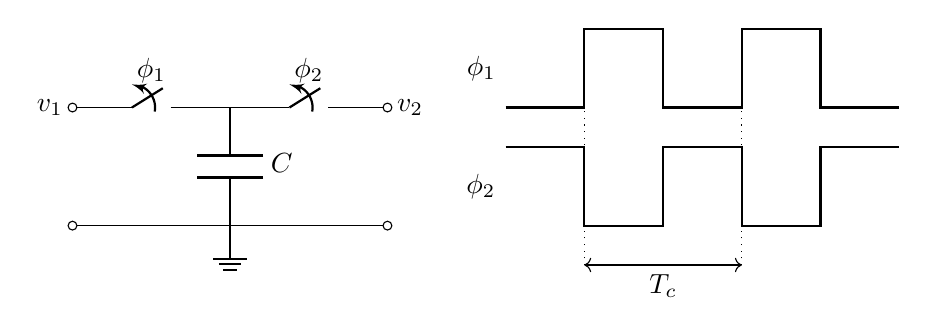
\begin{tikzpicture} \draw
        (0,0) node[left] {$v_1$} to[ospst=$\phi_1$, o-] (2,0)
        (2,0) to[C, l=$C$] (2,-1.5) node[ground] {}
        (2,0) to[ospst=$\phi_2$, -o] (4,0) node[right] {$v_2$}
        (0,-1.5) to[short, o-o] (4,-1.5)
        ;

        \begin{scope}[xshift=5.5cm, yshift=0cm] \draw
            (0,0.5) node[left] {$\phi_1$}
            [thick] (0,0) -- (1,0) -- (1,1) -- (2,1) -- (2,0) -- (3,0)
            -- (3,1) -- (4,1) -- (4,0) -- (5,0)
            
            (0,-1) node[left] {$\phi_2$}
            [thick] (0,-0.5) -- (1,-0.5) -- (1,-1.5) -- (2,-1.5) -- (2,-0.5) -- (3,-0.5)
            -- (3,-1.5) -- (4,-1.5) -- (4,-0.5) -- (5,-0.5);

            \draw [->] (2,-2) -- (3,-2);
            \draw [->] (2,-2) -- (1,-2);
            \draw (2,-2) node[anchor=north] {$T_c$};
            
            \draw [dotted] (1,-2) -- (1,1);
            \draw [dotted] (3,-2) -- (3,1);
        \end{scope}
    \end{tikzpicture}
    \caption{Basic principle of a switched-capacitor. Switches are usually implemented
    using MOS transistors. The two clocks $\phi_1$ and $\phi_2$ are non-overlapping.}
    \label{fig:switched-capacitor}
\end{figure}

\part{Voltage and current references}
Ideally, we would like voltage and current references to be as independent as
possible from
\begin{enumerate}
    \item the supply voltage $V_{CC}$ ;
    \item the temperature $T$.
\end{enumerate}
This part aims evaluating the performance of different architectures of
voltage and current references.

The reference for this part is~\cite[section~4.4]{gray}.

\section{Current reference}
\subsection{$V_{CC}$ reference}
\subsubsection{Current mirror}
The left part of figure~\ref{fig:current-mirror-widlar} shows an NPN current
mirror. This simple circuit produces a current $I_{OUT}$ given by
\[ I_{OUT} \approx I_{IN} = \frac{V_{CC}-V_{BE,1}}{R}. \]
Let's compute the sensitivity of $I_{OUT}$ to $V_{CC}$. Starting from the
definition of sensitivity, we have
\[ S^{I_{OUT}}_{V_{CC}} = \fpart{I_{OUT}}{V_{CC}}\frac{V_{CC}}{I_{OUT}} = \frac{V_{CC}}
{V_{CC}-V_{BE,1}} \approx 1 \]
where the last step step assumes $V_{CC} \gg V_{BE,1}$. We see that the output
current of the mirror current is strongly dependent from the supply voltage: the
sensitivity to $V_{CC}$ is 100\%. A good current reference should have a sensitivity
to the supply voltage in the order of 1\%.

\begin{figure}[ht]
    \centering
    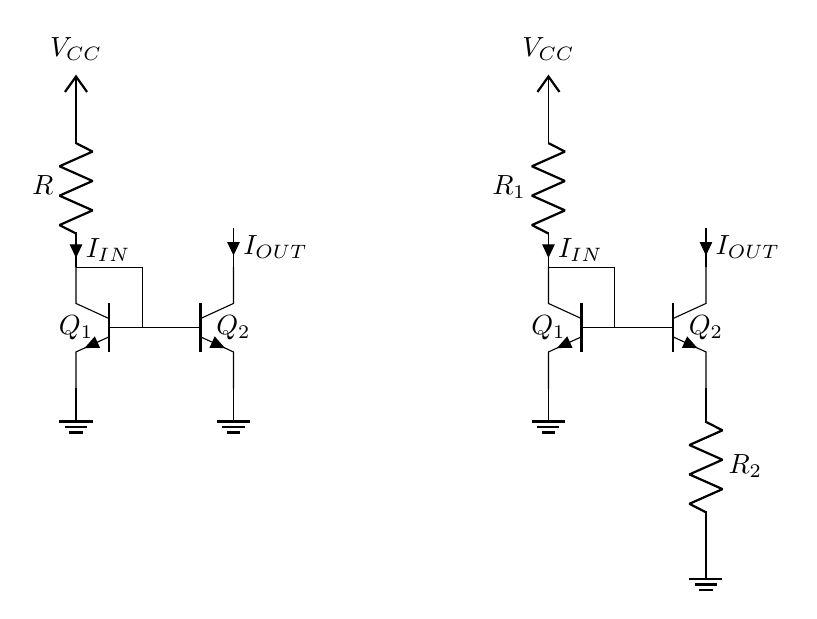
\begin{tikzpicture} \draw
        (0,0) to[Tnpn, name=q1, mirror, l=$Q_1$] (0,2)
        (q1.C) to[R, l=$R$, i<_=$I_{IN}$] ($(q1.C)+(0,2)$) node[vcc] {$V_{CC}$}
        (q1.E) node[ground] {}
        (q1.B) |- (q1.C)

        (2,0) to[Tnpn, name=q2, l=$Q_2$] (2,2)
        (q2.B) -- (q1.B)
        (q2.E) node[ground] {}
        ($(q2.C)+(0,0.5)$) to[short, i=$I_{OUT}$] (q2.C)

        (6,0) to[Tnpn, name=r1, mirror, l=$Q_1$] (6,2)
        (r1.C) to[R, l=$R_1$, i<_=$I_{IN}$] ($(r1.C)+(0,2)$) node[vcc] {$V_{CC}$}
        (r1.E) node[ground] {}
        (r1.B) |- (r1.C)

        (8,0) to[Tnpn, name=r2, l=$Q_2$] (8,2)
        (r2.B) -- (r1.B)
        (r2.E) to[R, l=$R_2$] ($(r2.E)-(0,2)$) node[ground] {}
        ($(r2.C)+(0,0.5)$) to[short, i=$I_{OUT}$] (r2.C)
        ;
    \end{tikzpicture}
    \caption{On the left, a simple BJT current source. On the right, a Widlar
    source. Note that these circuits can also be implemented using MOS transistors.}
    \label{fig:current-mirror-widlar}
\end{figure}

\subsubsection{Widlar source}
A Widlar source (see the right part of figure~\ref{fig:current-mirror-widlar})
improves the supply voltage sensitivity of its output current.
$I_{OUT}$ is given by\footnote{This is easy to derive knowing that the collector current
$I_C = I_s(e^{V_{BE}/V_T}-1) \approx I_se^{V_{BE}/V_T}$.}
\[ I_{OUT} \approx \frac{V_T}{R_2}\ln\frac{I_{IN}}{I_{OUT}}. \]
To compute $S^{I_{OUT}}_{V_{CC}}$, we take the derivative with respect to $V_{CC}$
of each side of the above equation
\[
    \fpart{I_{OUT}}{V_{CC}} = \frac{V_T}{R_2}\fpart{}{V_{CC}}\left(\ln{
    \frac{I_{IN}}{I_{OUT}}}\right).
\]
Developing this expression leads to
\[ S^{I_{OUT}}_{V_{CC}} = \frac{1}{1+\frac{I_{OUT}R_2}{V_T}}S^{I_{IN}}_{V_{CC}} \]
where $S^{I_{IN}}_{V_{CC}} \approx 1$.
\begin{myexem}
    Consider a Widlar source with $I_{IN} = \SI{1}{\milli\ampere}$, $I_{OUT} =
    \SI{5}{\micro\ampere}$ and $R_2 = \SI{27.4}{\kilo\ohm}$. In this case,
    $S^{I_{OUT}}_{V_{CC}} \approx 0.16$, this is already 6 times better than the
    basic current mirror. Generally speaking, a Widlar source is 5 to 10 times
    less sensitive to supply voltage than a current mirror.
\end{myexem}

\subsection{Other voltage standards}
Even though Widlar current sources offer better performance than simple current
mirrors in term of current sensitivity to supply voltage, they are still not adequate
for many types of analog circuits. Much lower sensitivity can be obtained by causing
the bias currents in the circuits to depend on a voltage standard other than the
supply voltage, for example, on $V_{BE}$ or $V_{TH}$, $V_T$ or the breakdown
voltage of a Zener diode. Each of these standards can be used to reduce supply
sensitivity. The drawback of the three first afermentioned standards, however, is
that they are temperature dependent:
\begin{itemize}
    \item $V_{BE}$ and $V_{TH}$ have a temperature coefficient of $\approx 1-\SI{2}
    {\milli\volt\per\degree}$ ;
    \item $V_T$ has a temperature coefficient of $k/q \approx \SI{86}{\micro\volt\per
    \degree}$.
\end{itemize}
The Zener diode has the disavantage that at least 7 to \SI{10}{\volt} of supply
voltage are required because standard integrated-circuit processes produce a
minimum breakdown voltage of about \SI{6}{\volt}.

\subsubsection{$V_{BE}$ or $V_{TH}$ reference}
The schematic of a base-emitter referenced current source is presented in
figure~\ref{fig:vbe-ref-current-source}. Assuming that transistor $Q_2$
supply enough current into $R_2$ so that a current flow in $Q_1$, we have
\[ V_{BE,1} = V_T\ln{\frac{I_{IN}}{I_{S1}}}. \]
If we neglect base currents, $I_{OUT}$ is equal to the current flowing through
$R_2$, that is
\[ I_{OUT} = \frac{V_{BE,1}}{R_2} = \frac{V_T}{R_2}\ln{\frac{I_{IN}}{I_{S1}}}. \]
Again, differentiating w.r.t $V_{CC}$ on both sides and rearranging a bit, we get
\[ S^{I_{OUT}}_{V_{CC}} = \frac{V_T}{I_{OUT}R_2}S^{I_{IN}}_{V_{CC}}
= \frac{V_T}{V_{BE(on)}}S^{I_{OUT}}_{V_{CC}}. \]
Assuming that $V_{CC} \gg 2V_{BE(on)}$, we have again that $S^{I_{OUT}}_{V_{CC}}
\approx 1$. With $V_{BE(on)} = \SI{0.7}{\volt}$,
\[ S^{I_{OUT}}_{V_{CC}} \approx 0.037 \]
which is again more than 4 times better than what we had with Widlar sources.

\begin{figure}[ht]
    \centering
    \begin{tikzpicture} \draw
        (0,0) to[Tnpn, name=r1, mirror, l=$Q_1$] (0,2)
        (r1.C) to[R, l=$R_1$, i<=$I_{IN}$] ($(r1.C)+(0,3)$) node[vcc] {$V_{CC}$}
        (r1.E) -- (0,-1) -- (1,-1) node[ground] -- (2,-1)
        to[R, l=$R_2$] (2,1)
        (r1.B) -- (2,1)
        to[Tnpn, name=r2, l=$Q_2$] (2,3)
        (r2.B) -- ($(r1.C)+(0,0.22)$)
        ($(r2.C)+(0,0.5)$) to[short, i=$I_{OUT}$] (r2.C)
        ;
    \end{tikzpicture}
    \caption{Base-emitter referenced current source. The same circuit can be
    implemented using MOS transistors (in this case it's called a threshold-referenced
    current course.}
    \label{fig:vbe-ref-current-source}
\end{figure}

\subsubsection{$V_{BE}$ or $V_{TH}$ self-biasing reference}
Power supply sensitivity can be greatly reduced by the use of self-biasing
circuits. The principle behind this technique is illustrated in
figure~\ref{fig:self-biasing-principle}. In a nutshell, the idea is to put
two constraints on the currents:
\begin{enumerate}
    \item Assuming the current mirror has unity gain, $I_{IN} = I_{OUT}$ ;
    \item The current source puts another constraints on $I_{IN}$ and
    $I_{OUT}$ of the same for as the one imposed by the base-emitter reference
    current source for example.
\end{enumerate}
The operating point must then be at the intersection of the two constraints
(see right part of figure~\ref{fig:self-biasing-principle}). There always
exists two possible operating point, a ideally unstable one when no current
is flowing in the circuit (point $B$) and a stable one (point $A$). In
practice, however, point $B$ is not unstable and the start-up circuit must
be used to avoid the circuit to stay at this point.

\begin{figure}
    \centering
    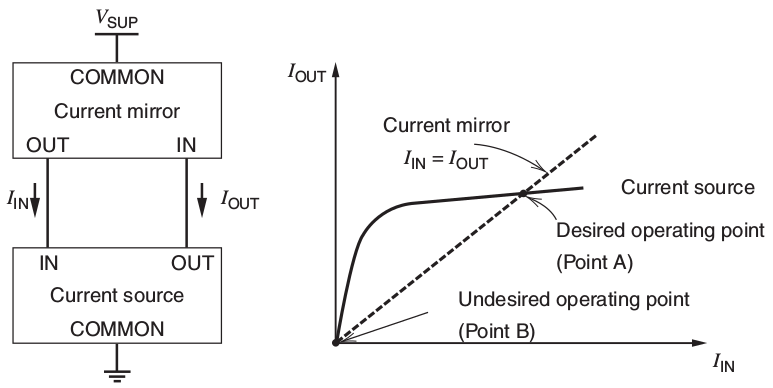
\includegraphics[width=0.7\textwidth]{figures/self-biasing-principle.png}
    \caption{Principle of a self-biased reference and determination of the
    operating point.}
    \label{fig:self-biasing-principle}
\end{figure}

\part{DAC}

\part{ADC}

\nocite{*}
\bibliographystyle{plain}
\bibliography{biblio}

\end{document}
